\PassOptionsToPackage{unicode=true}{hyperref} % options for packages loaded elsewhere
\PassOptionsToPackage{hyphens}{url}
%
\documentclass[
  12pt,
  twoside,
  banjiao]{ctexbook}
\usepackage{lmodern}
\usepackage{amssymb,amsmath}
\usepackage{ifxetex,ifluatex}

\usepackage{unicode-math}
\defaultfontfeatures{Scale=MatchLowercase}
\defaultfontfeatures[\rmfamily]{Ligatures=TeX,Scale=1}

% use upquote if available, for straight quotes in verbatim environments
\IfFileExists{upquote.sty}{\usepackage{upquote}}{}
\IfFileExists{microtype.sty}{% use microtype if available
  \usepackage[]{microtype}
  \UseMicrotypeSet[protrusion]{basicmath} % disable protrusion for tt fonts
}{}

\usepackage{xcolor}
\usepackage{subfig}
\usepackage{xurl} % add URL line breaks if available
\usepackage{bookmark}
\usepackage[version=4]{mhchem}
\usepackage{hyperref}
\usepackage{placeins}
\hypersetup{
  pdftitle={临床心电图详解与诊断},
  pdfauthor={github},
  pdfborder={0 0 0},
  breaklinks=true,
  bookmarksdepth=5}
\urlstyle{same}  % don't use monospace font for urls
\usepackage{longtable,booktabs}
% Allow footnotes in longtable head/foot
\IfFileExists{footnotehyper.sty}{\usepackage{footnotehyper}}{\usepackage{footnote}}
\makesavenoteenv{longtable}
\usepackage{graphicx,grffile}
\makeatletter
\def\maxwidth{\ifdim\Gin@nat@width>\linewidth\linewidth\else\Gin@nat@width\fi}
\def\maxheight{\ifdim\Gin@nat@height>\textheight\textheight\else\Gin@nat@height\fi}
\makeatother
% Scale images if necessary, so that they will not overflow the page
% margins by default, and it is still possible to overwrite the defaults
% using explicit options in \includegraphics[width, height, ...]{}
\setkeys{Gin}{width=\maxwidth,height=\maxheight,keepaspectratio}

\setlength{\emergencystretch}{3em}  % prevent overfull lines
% Redefines (sub)paragraphs to behave more like sections
\ifx\paragraph\undefined\else
  \let\oldparagraph\paragraph
  \renewcommand{\paragraph}[1]{\oldparagraph{#1}\mbox{}}
\fi
\ifx\subparagraph\undefined\else
  \let\oldsubparagraph\subparagraph
  \renewcommand{\subparagraph}[1]{\oldsubparagraph{#1}\mbox{}}
\fi

% set default figure placement to htbp
\makeatletter
\def\fps@figure{htbp}
\makeatother

\setcounter{secnumdepth}{5}
\usepackage{framed}
\usepackage{multirow}
\usepackage{ctex}
\usepackage{rotating}
\usepackage{tablefootnote}
\usepackage{caption}
\setCJKmainfont{思源宋体}
\setCJKfallbackfamilyfont{\CJKrmdefault}{宋体}
\setmainfont{思源宋体}
\usepackage[a4paper,top=1in, bottom=1in, left=0.8in, right=0.8in]{geometry}
\setlength{\parindent}{2em}
\setlength{\parskip}{0em}

%\newfontfamily\apostrophefont[Ligatures=TeX,Color=FF0000]{Liberation Serif}
\newfontfamily\apostrophefont[Ligatures=TeX]{Liberation Serif}
\XeTeXinterchartokenstate=1
\newXeTeXintercharclass \apostrophe

% Assign the new class to all Latin capital letters
\makeatletter
\@tempcnta=`'
\loop\unless\ifnum\@tempcnta>`'
  \XeTeXcharclass \@tempcnta \apostrophe
  \advance \@tempcnta by 1
\repeat
\makeatother

% Setup font change
\XeTeXinterchartoks 0 \apostrophe   = {\begingroup\apostrophefont}
\XeTeXinterchartoks \apostrophe 0   = {\endgroup}
\XeTeXinterchartoks 4095 \apostrophe = {\begingroup\apostrophefont}
\XeTeXinterchartoks \apostrophe 4095 = {\endgroup}

\renewcommand {\thetable} {\thechapter{}-\arabic{table}}
\renewcommand {\thefigure} {\thechapter{}-\arabic{figure}}
\newcommand\subsectiontitleformat[1]{\noindent 【#1】}

\ctexset {
  section = {
    name
    = {第,节},
    number = \chinese{section},
  },
  subsubsection = {
    name 
    = {(,)},
    number = \chinese{subsubsection}
  },
  subsection = {
    name 
    = {,、},
    number = \chinese{subsection}
  }
}


\title{临床心电图详解与诊断}
\author{github \\ 项目主页:\url{https://github.com/scienceasdf/medical-books}\\ 新书下载:\url{https://github.com/scienceasdf/medical-books/releases/latest}}


\begin{document}
\maketitle
\frontmatter
{
\setcounter{tocdepth}{1}
\tableofcontents
\addcontentsline{toc}{chapter}{目录}
}
\newpage

\mainmatter
\part{常见急症状的诊断思路与处理原则}

\chapter{发热及超高热危象}

发热(fever)是指某个人的体温因各种原因超过正常范围,见于各种全身性和局部性感染以及许多非感染性疾病(如肿瘤与结缔组织病等),它是内科急诊中最常见的症状。一般而言,当腋下、口腔或直肠内温度分别超过37℃、37.3℃和37.6℃,并且24小时内温度差波动在1℃以上,可称为发热。按照发热的高低,可分为:①低热:37.4~38℃;②中度发热:38.1~39℃;③高热:39.1~41℃;④超高热或过高热:41℃以上。

超高热或过高热危象(extreme pyrexic
crisis,EPC)是指过高热若不及时处理,使脑、心、肾等重要器官受到严重损害,出现抽搐、昏迷、休克、出血、心力衰竭、呼吸衰竭和肾功能衰竭等危及生命的状态。若抢救不力,常于数小时内死亡。

\subsection{体温的调节与发热的机制}

正常人的体温是由体温调节中枢通过神经、体液因素调节产热和散热过程,保持产热和散热这对矛盾的动态平衡,所以正常人体有相对恒定的体温。口腔温度一般维持在37℃上下,波动范围36.3~37.2℃;直肠内温度一般比口腔内温度约高0.3~0.5℃,腋窝温度比口腔内温度约低0.2~0.4℃。不同个体的正常体温也会略有差异,少数健康成人口腔温度可稍低于36.3℃或稍高于37.2℃。正常人体温在24小时内有轻微的波动,晨间稍低,下午稍高,相差不超过1℃。在不同的生理状态下,体温也有轻微差异。小儿因代谢率高,其体温可较成年人稍高;老年人体温可较青壮年低。妇女月经期体温比平日为低,而在排卵期与妊娠期则稍高。此外,进食、剧烈运动、突然进入高温环境、情绪激动等因素也可使体温稍有上升。

人体内产热除基础代谢产热外,静止状态下组织代谢也产生热量。体力活动时,脂肪及糖分解是体内产热的主要来源。运动时骨骼肌和皮肤的产热量可占全身产热量的70\%。随着外界温度的降低,机体在减少散热的同时增加代谢率,成人主要通过寒战反应产热,它可最大量地增加产热,以补充机体在寒冷环境中丧失的体热;新生儿在寒冷环境下刺激交感神经兴奋,使脂肪代谢成脂肪酸,供给机体产热。皮肤在寒冷时血管收缩,减少体表和肢体末端向外界散发热量。另外,皮肤表面遇寒冷刺激时产生竖毛肌反应,借助于围绕体表密闭的空气静止层来保存热量。

人体散热主要有辐射、传导、对流及蒸发四个物理过程,当周围温度低于皮肤温度时,皮肤即辐射散热;其次是体内热量传导至皮肤周围空气层,经对流散热。当周围温度超过体温时,主要依靠汗液蒸发散热。体热从皮肤、呼吸道和大小便3处消散,以皮肤散热最为重要。当室温在23~25℃时,体热通过皮肤辐射、对流、传导散热占70\%;当室温高达31~32℃时,出汗蒸发即成为散热主要方式。皮肤血管内血流量越大,散热速度越快;体表温度越高,则散热也越迅速。

健康人的产热与散热处于平衡状态。产热与散热过程均受在下丘脑的体温调节中枢的调控。下丘脑的体温调节中枢存在着与恒温箱温度调节器相类似的调定点(set
point),此调定点的高低决定体温的水平。体温调节中枢调定点上移,中心温度低于调定点时,调定点的冲动发放,调温指令抵达产热和散热器官,一方面通过运动神经引起骨骼肌的张力增加或寒战,使产热增多;另一方面经交感神经系统引起皮肤血管收缩,使散热减少,最终导致发热。

体温升高有发热与高温(hyperthermia)之分,高温是由散热障碍或产热过多引起,一般与体温调节中枢无关:①散热障碍:可因药物(抗精神病药物、阿托品中毒等)、外界高温(中暑)及内源性代谢热(如甲亢危象)等引起,在湿热环境中更容易发生。超高热是体温升高至体温调节中枢所能控制的调定点以上,达到特别高的水平(>
41℃),见于脑炎、脑出血、颅内病变、中暑等疾病。②产热过多:见于对某些麻醉药物过敏患者所产生的恶性高温(malignant
hyperthermia),由于肌细胞不受控制地大量释放热原所致。另外,除功能性低热外,其余原因所致的发热皆可能与致热原(pyrogen)作用于下丘脑体温调节中枢有关。

致热原是一类能引起恒温动物体温异常升高的物质的总称。可分为外源性和内源性两类,前者包括各种病原体如细菌、病毒、立克次体、衣原体、螺旋体、原虫和寄生虫等的毒素及其代谢产物,尤以内毒素(多属脂多糖类物质)最为重要,其次是原胆烷醇酮、多核苷酸、抗原-抗体复合物等;后者包括白细胞介素(如IL-1,IL-2、IL-6等)、肿瘤坏死因子(TNF)和干扰素等,其中IL-1为内源性致热原的主要成分。外源性致热原一般不能直接作用于体温调节中枢引起发热,但能刺激和激活主要存在于白细胞、单核细胞和组织吞噬细胞内的内源性致热原前体,于短期内合成新的mRNA和致热原,这些具有活性的内源性致热原可能是通过某些生物活性物质如前列腺素、单胺、cAMP、钙钠比值、内啡肽等作为中介,提高体温调节中枢调定点而引起发热。例如,IL-1它主要来源单核细胞和巨噬细胞,这些细胞平时仅含有微量内源性致热原,但并不自动释放,只有在受到外源性致热原激活后,合成增多,才释放出来。IL-1作用于下丘脑的血管内皮细胞,产生花生四烯酸代谢产物,主要是前列腺素E\textsubscript{2}
(PGE\textsubscript{2}
),后者是前列腺素中最强有力的致热物质,促使下丘脑调定点升高。体温中枢调定点上移,体温低于调定点时,调定点的冲动发放,通过血管运动中枢和周围传出神经使血管收缩和血流减少,肌肉张力增加甚至发生寒战,使散热减少或产热增多,最终导致发热。

高温的发生机制与发热不同,是因产热、散热异常所致。因产热过多引起的发热不多,主要见于剧烈运动后、癫痫持续状态和甲亢危象时,一般持续不久。广泛性皮肤病、阿托品中毒时出汗功能障碍,散热减少引起发热,主要见于炎热季节。大量失水、失血常伴有发热,尤其多见于小儿,出现所谓“失水热”,是由于血容量减少、散热减少。心脏病患者也可有发热,主要由于肺部充血和肺部感染或有风湿活动或血栓形成,此外,在心力衰竭阶段的发热,则与皮肤水肿引起散热减少有关。中枢神经性高温以中暑最为典型,也可由脑出血、脑炎等引起。由于中枢神经系统遭受严重伤害,下丘脑丧失调温能力而衰竭,会有骤升的超高温,达41℃或以上,同时交感神经受抑制,以皮肤干燥无汗为特征。

\subsection{诊断思路}

\subsubsection{病史}

详细询问病史对于发热原因的诊断常能提供重要线索。此外,对发热患者定期检测体温,密切观察热度的高低、时限、热型等也有重要价值。

\subparagraph{起病方式}

一般而言,急性感染性疾病起病多较急骤,常有受凉、疲劳、外伤或进食不洁食物等病史。若发热前有明显寒战者,多属化脓性细菌感染或疟疾;而一般非感染性发热,以及结核、伤寒、立克次体和病毒感染多无寒战。

\subparagraph{发热的分期与分型}

发热的临床经过一般分为以下3期:

\hypertarget{text00008.htmlux5cux23CHP1-1-2-1-2-1}{}
(1) 体温上升期:

表现为疲乏、不适感、肌肉酸痛、皮肤苍白、干燥、无汗、畏寒或寒战等症状。体温上升有两种形式:①骤升型:体温在数小时内达39~40℃以上,常伴有寒战。②缓升型:体温于数日内缓慢上升达高峰。

\hypertarget{text00008.htmlux5cux23CHP1-1-2-1-2-2}{}
(2) 高热持续期:

此时体温已达高峰,临床表现为皮肤潮红而灼热,呼吸加快加强,可有出汗。此期持续数小时、数天或数周。其热型(体温曲线)可表现为:①稽留热(continued
fever):体温持续于39~40℃左右,达数天或数周,24小时波动范围不超过1℃。见于肺炎、伤寒、斑疹伤寒(早期)等。②弛张热(remittent
fever):体温在39℃以上,但波动幅度大,24小时内体温差达2℃以上,体温最低时一般仍高于正常水平。见于脓毒血症、风湿热、重症结核、化脓性炎症如肝脓肿等。③间歇热(intermittent
fever):高热期与无热期交替地出现。体温波动幅度可达数度。无热期(间歇期)持续1天乃至数天,反复发作。见于疟疾、急性肾盂肾炎、局限性化脓性感染等。④回归热(recurrent
fever):体温急骤升高至39℃以上,持续数天后又骤然下降至正常水平,高热期与无热期各持续若干天,即规律地互相交替一次。见于回归热、霍奇金病、周期热等。⑤波状热(undulant
fever):体温逐渐升高达39℃或以上,数天后又逐渐下降至正常水平,数天后又逐渐升高,如此反复多次,常见于布鲁菌病、恶性淋巴瘤等。⑥不规则热(irregular
fever):发热持续时间不定,变动无规律,可见于肺结核、感染性心内膜炎等。

应予以强调的是,目前由于抗生素的广泛应用(包括滥用),或由于应用(包括不适当应用)解热药、肾上腺皮质激素等,使上述典型热型已不常见。此外,热型也与机体反应性有关,年老体弱者由于反应性差,即使化脓性细菌感染也常无寒战、高热,而表现为低热甚至不发热。

\hypertarget{text00008.htmlux5cux23CHP1-1-2-1-2-3}{}
(3) 体温下降期:

由于机体的防御功能与适当的治疗,疾病得到控制,体温恢复正常。体温下降的方式有两种:①骤降(crisis):体温于数小时内迅速降至正常,有时可低于正常,常伴有大汗。常见于疟疾、急性肾盂肾炎、肺炎及输液反应等。②渐降(lysis):体温于数天内逐渐降至正常。如伤寒、风湿热等。

\subparagraph{重视发热的伴随症状}

在询问病史时,应当重视具有定位意义的伴发的局部症状,以便确定主要病变在哪个系统。如发热伴有鼻塞流涕、咽痛、咳嗽,而一般情况良好者多为上呼吸道感染,若有胸痛、咯铁锈色痰和呼吸困难者,则多为下呼吸道感染,如肺炎。发热伴神经系统症状,如头痛、呕吐、昏迷、惊厥、脑膜刺激征等则表示病变在中枢神经系统,应考虑各种脑膜炎、脑炎、中暑、急性脑卒中等;但儿童易有高热惊厥,不一定有严重脑部病变。发热伴有肋椎角、腰肋部疼痛及尿频、脓尿、血尿者提示多为泌尿系统感染。发热伴有明显关节痛或关节炎症状者应多考虑风湿热等结缔组织疾病。发热伴有恶心呕吐、腹痛、腹泻者,应多考虑急性胃肠道炎症。发热、黄疸伴右上腹痛应注意肝胆感染。依此类推。

除上述病史外,还应重视流行病学资料,如患者来自的地区、年龄、性别、职业、发病季节、旅游史、接触感染史等,尤其是传染病的流行病学史非常重要。如布鲁菌病多见于从事畜牧业(尤其是动物接生)的人群中;同性恋者及静注毒品成瘾者的发热待查以艾滋病或合并机会性感染的可能性较大。

\subsubsection{体格检查}

遇急重发热患者,应首先测呼吸、脉搏、血压等重要生命体征,并快速进行全面的体格检查,重点检查皮肤、黏膜有无皮疹、瘀点以及肝、脾、淋巴结肿大等。发热伴有中毒性休克时,患者面色青灰、脉细速、血压下降或测不出,见于休克型肺炎、暴发性流行性脑脊髓膜炎、中毒性菌痢、脓毒症、流行性出血热等。

\subparagraph{面容}

一般急性感染多呈急热面容。伤寒、副伤寒者常表情淡漠,即所谓“伤寒面容”。斑疹伤寒、恙虫病、流行性出血热患者常呈醉酒样面容。猩红热患者见口周苍白。麻疹患者常见眼睑水肿、结膜充血、分泌物增多等。急性白血病、再生障碍性贫血和恶性组织细胞病常因贫血亦可呈面色苍白。发热伴面部蝶形红斑是播散性红斑狼疮的特殊病症。口唇疱疹可见于大叶性肺炎、间日疟、流行性脑脊髓膜炎、流行性感冒、大肠埃希菌败血症等。

\subparagraph{皮肤特征}

注意有无皮疹及出血点。皮肤多汗可见于结核病、风湿热、败血症、恶性淋巴瘤。皮肤发疹可见于猩红热、麻疹、风疹、斑疹伤寒、伤寒、水痘、恙虫病、传染性单核细胞增多症、丹毒、红斑狼疮、急性皮肌炎等,根据其特征性皮疹及出疹日期可对急性发疹性传染病作出诊断(表\ref{tab1-1})。皮疹还见于风湿热、药物热、渗出性红斑、结节性红斑、血清病等。出血性皮疹或出血素质常提示重症感染或血液病,前者包括脓毒症、流行性脑脊髓膜炎、感染性心内膜炎、流行性出血热、登革热、重症肝炎和钩端螺旋体病等;后者包括白血病、急性再生障碍性贫血和恶性组织细胞病等。皮肤或软组织有化脓性病灶,常提示为发热原因,或脓毒症的来源。发热伴皮肤黄染(黄疸)要注意胆道感染、钩端螺旋体病、重症肝炎和急性溶血等。

\subparagraph{淋巴结肿大}

全身性淋巴结肿大是原发性淋巴组织病变或全身性感染的病征,如伴周期发热是霍奇金病的临床特征,如伴不规则发热,应注意传染性单核细胞增多症、结核病、急性淋巴细胞性白血病、恶性组织细胞病等。局部淋巴结肿大常提示局部有急性炎症,如口腔和咽部感染常有颌下淋巴结肿大,下肢感染可有腹股沟淋巴结肿大等。但也有例外,如急性出疹性发热病伴耳后、枕骨下淋巴结肿痛,提示风疹的诊断。

\subparagraph{脾肿大}

发热伴脾肿大者见于脓毒症、伤寒、病毒性肝炎、疟疾、黑热病、感染性心内膜炎、布鲁菌病、血吸虫病、淋巴瘤、恶性组织细胞病、白血病等。

\subparagraph{发热伴有胸部体征}

如闻及肺部干湿性啰音或实变体征等,应考虑呼吸系统感染;发热伴有栓塞、心脏杂音,尤其是原有器质性心脏病者心脏杂音发生明显改变时,应注意感染性心内膜炎;发热伴心包摩擦音或心包积液体征,常提示心包炎。而急性心肌炎常表现为发热与心率不成比例,心率增快常超过发热程度。

\subparagraph{肌肉与关节}

发热伴肌肉疼痛见于许多传染病,一般无特殊性诊断意义,但如腓肠肌剧烈疼痛,甚至不能站立或行走,常提示钩端螺旋体病。局部肌痛兼有发热与白细胞增多,须检查有无深部脓肿,尤其是药物肌肉注射引起的臀肌无菌性脓肿。发热伴多关节肿痛,病因常为各种关节炎,如化脓性、感染中毒性与变态反应性等,而淋病性与结核性关节炎常侵犯单个的大关节。

长期不明原因的发热患者尤应注意隐蔽性病灶,如肝脏、膈下、脊椎、盆腔、鼻窦、乳突等局部脓肿。肝脓肿是引起长期发热的常见病因,在早期不一定有局部症状。脊椎病变如结核或脓毒症后脊椎旁化脓性病灶在体检时易被忽略。眼底检查与肛门指检应作为常规,粟粒性结核可有眼脉络膜结核结节,年老患者肛门指检可发现前列腺脓肿。此外,腹部与盆腔手术(包括引产)后发热可由腹腔或盆腔内隐蔽的脓肿引起。

\subsubsection{辅助检查}

对发热患者行辅助检查时必须掌握检查目的明确,并以简便快捷为原则。对于通过病史询问和体检能确诊者不一定均作有关检查。常用的辅助检查包括:①血、尿、粪常规检查。②血清学检查:如肥达反应、外斐反应、钩端螺旋体病的凝集溶解试验,乙脑的补体结合试验,系统性红斑狼疮的抗核抗体试验等。③血或骨髓培养:对伤寒、副伤寒、脓毒症、细菌性心内膜炎等疾病的病原诊断均具有决定性意义。④X线、CT与MRI检查:CT与MRI检查对诊断骨盆内、膈下与腹腔深部隐蔽性脓肿,尤其对发现腹膜后病灶如淋巴瘤、脓肿、血肿等有重要价值。⑤超声检查:对疑有急性渗出性心包炎和感染性心内膜炎患者,可行超声心动图检查。腹部超声波检查适用于疑有腹腔内占位性病变、肝脓肿、肝胆道结石以及肾脓肿、泌尿系结石等患者。⑥活体组织检查:如肝穿刺活组织检查、淋巴结以及皮损与皮下结节活体组织检查等。骨髓检查对白血病、恶性组织细胞病等具有决定性诊断价值。

\begin{table}[htbp]
\centering
\caption{急性发热伴发疹性疾病的皮疹}
\label{tab1-1}

\includegraphics[width=6.625in,height=3.95833in]{./images/Image00003.jpg}
\end{table}

\subsubsection{病因诊断}

发热是由于各种原因导致机体产热过多或散热减少,以及体温中枢功能障碍所致。其原因很多且复杂。在临床实践中,以发热为主诉或唯一症状就诊者有急性发热,尤其出疹性发热,原因不明发热,长期低热,超高热与反复发热。其病因特征亦各异。

\subparagraph{急性发热}

热程在2周以内的发热称为急性发热。其原因很多,绝大多数属于感染,尤以呼吸道、泌尿道和消化道感染最常见,因为这些系统与外界相通,最易遭受病原体的侵袭。在排除上述系统感染后,则要注意某些急性传染病和其他系统的感染。一般而言,这类发热,常伴有定位症状,比较容易诊断。

\subparagraph{长期}

“不明原因”的中、高热
系指发热持续3周以上,体温多次超过38.3℃,经过至少1周深入细致的检查仍不能确诊的一组疾病,称为原因不明发热(fever
of unknown
origin,FUO)。其病因在不同年代和不同地理区域明显不同,但主要有感染、恶性肿瘤与结缔组织-血管性疾病三大类,共约占长期发热病因的80\%~90\%。其中由感染引起的长期发热在国内占60\%~70\%,在其他发展中国家更高些,而在发达国家约占总数1/3。由于人的寿命延长,传染病逐渐减少,恶性肿瘤引起的发热比例有增高趋势,国内约占20\%。结缔组织-血管性疾病约占10\%。病因也受年龄的影响:6岁以下的FUO患儿以感染性疾病为主,尤其是原发性上呼吸道、泌尿道感染或全身感染;6~14岁年龄组则以结缔组织-血管性疾病和小肠炎症性疾病为最常见的病因;14岁以上的成人组,虽然仍以感染性疾病占首位,但肿瘤性疾病明显增多。仍有10\%的病例始终原因不明。

\hypertarget{text00008.htmlux5cux23CHP1-1-2-4-2-1}{}
(1) 感染:

引起发热待查的感染性疾病中主要由细菌感染所致,而任何一种致病菌或条件致病菌,或L-型细菌性感染均可分为全身性与局部性感染。全身性感染以伤寒与副伤寒、粟粒型结核与播散性结核(包括腹膜、肠、肠系膜淋巴结、肝、肾、胸膜和肺与肺门淋巴结结核)、脓毒症与感染性心内膜炎、布鲁菌病、黑热病、急性血吸虫病、旋毛虫病等;局部性感染以肝脓肿、胆道与泌尿生殖道感染、腹腔内脓肿(包括肝下、膈下、结肠旁、阑尾周围、腹膜后、盆腔脓肿等)为常见。局部性感染易被临床忽略。

\hypertarget{text00008.htmlux5cux23CHP1-1-2-4-2-2}{}
(2) 恶性肿瘤:

也是长期发热的常见原因。最常见的为原发性肝癌、淋巴瘤、恶性组织细胞病与白血病,其次为实质性恶性肿瘤如肺癌、肾癌、甲状腺癌等。

\hypertarget{text00008.htmlux5cux23CHP1-1-2-4-2-3}{}
(3) 结缔组织-血管性疾病:

也是较常见原因之一,大多伴有关节痛、皮肤、心、肾等多系统病变引起的相应症状与体征,但少数病例在典型症状出现前数周或数月可出现发热。此类疾病以系统性红斑狼疮、成人少年型类风湿关节炎、多动脉炎、皮肌炎、混合性结缔组织病、风湿热等常见。

\hypertarget{text00008.htmlux5cux23CHP1-1-2-4-2-4}{}
(4) 其他:

肉芽肿性疾病(肉芽肿性肝炎、结节病、局限性回肠炎等)、药物热、伪装热、体腔积血如血胸、血腹、肺梗死等。

\subparagraph{长期低热}

系指口腔温度在37.5~38.4℃,持续4周以上者。在诊断为长期低热时,必须先了解其正常体温,排除生理或功能性因素,并排除高温环境等影响,如在高温车间的纺织女工中,有长期低热者可达10\%以上。长期低热由感染性疾病引起者占40\%,非感染性疾病占57\%,原因不明占3\%。长期低热的原因可分为器质性与功能性两大类:

\hypertarget{text00008.htmlux5cux23CHP1-1-2-4-3-1}{}
(1) 器质性低热:

①慢性感染:如结核病、肝脏疾病、慢性肾盂肾炎、慢性胆道感染以及各种病灶感染(鼻窦炎、牙根脓肿、前列腺炎、慢性盆腔炎、肛门周围脓肿等)。②结缔组织疾病:如风湿热、类风湿关节炎、系统性红斑狼疮等。③内分泌疾病:如甲亢、嗜铬细胞瘤等。④恶性肿瘤:早期淋巴瘤、实质性癌肿转移等。

\hypertarget{text00008.htmlux5cux23CHP1-1-2-4-3-2}{}
(2) 功能性低热:

①生理性低热:月经前期低热、妊娠期低热等。②神经功能性低热:多见于青年女性,长期低热可长达数月或数年。有些患者低热有季节性,出现于夏季(谓之夏季低热),且每年如此。体温在一昼夜内波动幅度较小,常不超过0.5℃,且口腔、腋窝与直肠温度差不大,甚至可出现腋温大于口温,口温大于肛温或腋温大于肛温的反常现象,两侧腋温可相差1℃以上。体温昼夜规律失常。患者常伴有脸色潮红、皮肤划痕症、心动过速等自主神经功能紊乱或神经症色彩。但患者一般情况好,体重无变化,虽经各种药物治疗无效,但不经治疗也可自行消退。神经功能性低热较常见,约占长期低热的1/3,预后良好。③感染后低热:急性病毒或细菌感染得到控制后,高热消退,但可出现持续较久的低热,并伴有乏力,纳差等现象。此种发热可能与体温调节中枢功能失常或自主神经功能紊乱有关。

\subsubsection{超高热危象的识别与诊断}

超高热系指发热超过41℃以上,主要见于体温调节中枢功能障碍,有以下各种原因:①中暑或日射病;②脑部疾病:如严重脑外伤、脑出血、脑炎与脑肿瘤等;③输血、输液污染引起严重致热原反应与脓毒症;④麻醉药引起的恶性高热;⑤临终前超高热等。不论病因如何,超高热对细胞膜与细胞内结构有直接损害作用,当深部体温>
41℃时细胞线粒体的氧化磷酸化出现障碍,可引起永久性脑损害;42~43℃持续数分钟细胞会陷入不可逆的损害,涉及全身各种细胞,尤以脑、心、肝、肾的变化最为突出,容易造成脑水肿颅内压升高,抽搐、昏迷,心、肝、肾、肺功能衰竭,DIC等多脏器功能衰竭。超高热危象的诊断要点是:

\subparagraph{超高热}

超高热(体温> 41℃)是超高热危象的必有表现。

\subparagraph{超高热时伴有多脏器功能受损害的表现}

①心血管系统:低血压休克、心功能不全、心肌缺血与心律失常等。②中枢神经系统:体温越高对中枢神经系统损害越重,症状出现越早;包括不同程度的意识障碍如谵妄、嗜睡、昏迷、抽搐、大小便失禁、脑膜刺激征、瘫痪、病理反射阳性、脑疝、视神经乳头水肿等。③凝血功能障碍:早期出现凝血酶原时间延长,纤维蛋白原减少,血小板减少,出血时间、凝血时间延长;晚期常有广泛而严重的出血、DIC形成。这与过高热直接损害毛细血管、渗透性增加,肝功能受损凝血因子减少,骨髓受损血小板减少等有关。④肾功能损害:可有血尿、管型、少尿、无尿、血肌酐升高等肾功能不全的表现。⑤肝功能损害:肝功能异常如ALT升高、血清胆红素升高,甚至表现为急性肝功能衰竭。⑥水电解质和酸碱平衡失调。⑦其他表现:如横纹肌溶解可致血肌酸磷酸激酶(CK)增高等。

\subparagraph{原发病的表现}

如中毒性菌痢的腹泻、脓血便;乙脑时的抽搐、昏迷等。

\subsection{处理原则}

\subparagraph{支持治疗}

患者出现神志改变、呼吸窘迫、血流动力学不稳定等危及生命的症状与体征时,立即实施监护、建立静脉通路、气道管理、补液以及氧疗,必要时予以呼吸支持治疗。

\subparagraph{超高热危象的处理}

超高热和超高热危象是短暂的临床表现,经适当处理可能很快恢复(如中暑、输液反应等),亦可很快死亡(恶性高温)。早期诊断与早期处理同预后直接有关。因此,对每个可能发生超高热的患者应随时检测体温,一旦出现超高热,应以最快的速度降低中心体温、代谢率,以打断超高热引起的恶性循环,同时防治各种并发症。其中,降温是抢救超高热危象的主要措施。降温速度决定预后,应在1小时内使直肠温度降至38.5℃以内。具体降温措施详见本书第129章“中暑”。

\subparagraph{对症处理}

发热的对症治疗包括:①物理降温:一般可用冷毛巾湿敷额部,每5~10分钟更换1次,或用冰袋置于额、枕后、颈、腋和腹股沟处降温,或用25\%~50\%酒精擦浴。或头置冰帽、冰水灌肠、冷盐水洗胃,或将患者置于空调房内(使室温维持在27℃左右)。应根据具体条件选用。②药物降温:视发热程度可采用口服或肌注解热镇痛药。常用的口服解热镇痛药有:阿司匹林(0.3~0.6g/次)、对乙酰氨基酚(0.3~0.5g/次)、布洛芬(0.2~0.4g/次)、安乃近(0.25~0.5g/次)、解热止痛片(APC片,1~2
片/次)、速效伤风胶囊(1~2粒/次)、复方对乙酰氨基酚片(1~2片/次)等。常用的注射用解热镇痛药有:阿司匹林精氨酸盐(0.5~1.0g/次)、阿司匹林赖氨酸盐(赖氨匹林,0.9~1.8g/次)、对乙酰氨基酚(0.15~0.25g/次)、息热痛注射液(2ml/次)、安痛定注射液(1支/次)等。高热者病情需要时可短期应用肾上腺皮质激素,如地塞米松5~10mg静注或肌注;或以地塞米松12~20mg/d或氢化可的松300~600mg/d静滴。

\subparagraph{抗生素经验性应用}

对感染病例早期抗生素经验性应用是有益的。一般来讲,若有明确的病原菌感染,则选择覆盖特定病原菌感染的窄谱抗生素;若不明确,可选择覆盖革兰阳性和革兰阴性需氧菌、厌氧菌的广谱抗生素。

\subparagraph{诊断性治疗}

当发热病因一时难以查明时,在不影响进一步检查的情况下,可按可能性较大的病因进行诊断性治疗(如疑疟疾,可试用氯喹;疑阿米巴性肝脓肿,行抗阿米巴治疗;疑结核病行抗结核治疗时间以3~4周以上为宜),期望获得疗效而做出临床诊断。诊断性治疗应选用特异性强、疗效确切及安全性大的治疗药物,剂量应充足并完成整个疗程,无特殊原因不得随便更换试验药物。

\subparagraph{随访观察}

对部分症状轻微、经过详细检查仍不能明确病因的发热待查患者,也可在专科门诊进行长期随访而不作特殊处理,确有不少患者可获自愈。

\protect\hypertarget{text00009.html}{}{}

\hypertarget{text00009.htmlux5cux23CHP1-1-4}{}
参 考 文 献

1. 陈灏珠 ,林果为.实用内科学.第13版.北京:人民卫生出版社,2009:332

2. 陈文彬 ,潘祥林.诊断学.第7版.北京:人民卫生出版社,2008:16

3.
陈新谦,金有豫,汤光.新编药物学.第17版.北京:人民卫生出版社,2011:179

\protect\hypertarget{text00010.html}{}{}

\chapter{意识障碍和昏迷}

意识是指人体对周围环境及自身状态的感知能力。意识障碍(disturbance of
consciousness)是脑和脑干功能活动的抑制状态。按照生理与心理学基础可将意识障碍分为觉醒障碍(觉醒度下降,即狭义的意识障碍)和意识内容障碍两大类。前者表现为嗜睡、昏睡和昏迷;后者表现为意识模糊和谵妄等。脑和脑干功能活动的不同抑制程度决定了不同的意识障碍水平。

昏迷(coma)是一种最为严重的意识障碍。患者意识丧失,运动、感觉、反射和自主神经功能障碍,给予任何刺激(如语言、声音、光线、疼痛等)均不能将患者唤醒,但生命体征如呼吸、脉搏、心跳、血压和体温尚可存在。昏迷是病情危重的信号,是常见危重急症,病死率高,临床医师如能迅速作出正确的诊断和及时的处理,患者往往可能转危为安。

以觉醒度改变为主的意识障碍,根据检查时刺激的强度和患者的反应,可分为以下三级:

嗜睡(drowsiness):主要表现为病理性睡眠过多过深,能被各种刺激唤醒,并且能够正确回答问题和做出各种反应,但当刺激去除后又很快入睡。

昏睡(stupor):是一种比嗜睡深而又较昏迷稍浅的意识障碍。昏睡时觉醒水平、意识内容及随意运动均减至最低限度。患者不能自动醒转,在持续强烈刺激下能睁眼、呻吟、躲避,可作简短而模糊的回答,但反应时间持续很短,很快又进入昏睡状态。昏睡时可见到运动性震颤、肌肉粗大抽动、不宁或刻板的动作、强握和吸吮反射。

昏迷(coma):患者意识完全丧失,各种强刺激不能使其觉醒,无有目的的自主活动,不能自发睁眼。昏迷按严重程度可分为浅昏迷、中昏迷和深昏迷三级:①浅昏迷(mild
coma):即轻度昏迷。仅对剧痛刺激(如压迫眶上神经)有防御性反应和痛苦表情,不能言语,可有无意识的自发动作,各种生理反射存在(如吞咽、咳嗽、角膜和瞳孔对光反射),呼吸、血压、脉搏一般无明显改变。②中昏迷:对外界的正常刺激均无反应,自发动作很少。对强烈刺激可有防御反射,角膜反射减弱,瞳孔对光反射迟钝,眼球无转动,大小便潴留或失禁。呼吸、血压、脉搏已有变化。③深昏迷(deep
coma):对外界的任何刺激均无反应,全身肌肉松弛,无任何自主运动。眼球固定,瞳孔散大,各种反射全部消失,大小便多失禁。生命体征已有明显改变,呼吸不规则,血压或下降。

以意识内容改变为主的意识障碍常见有以下三种:

意识模糊(confusion):表现为注意力减退,情感反应淡漠,定向力障碍,活动减少,语言缺乏连贯性,对外界刺激可有反应,但低于正常水平。

精神错乱(psychoderangement):患者对周围环境的接触程度障碍,认识自己的能力减退,思维、记忆、理解与判断力均减退,言语不连贯并错乱,定向力亦减退。常有胡言乱语、兴奋躁动。

谵妄状态(delirium):表现为意识内容清晰度降低,伴有睡眠-觉醒周期紊乱和精神运动性行为。除了上述精神错乱以外,尚有明显的幻觉、错觉和妄想。幻觉以视幻觉最为常见,其次为听幻觉。幻觉的内容极为鲜明、生动和逼真,常具有恐怖性质。因而,患者表情恐惧,发生躲避、逃跑或攻击行为,以及运动兴奋等。患者言语可以增多,不连贯或不易理解,有时则大喊大叫。谵妄或精神错乱状态多在晚间加重,也可具有波动性,发作时意识障碍明显,间歇期可完全清楚,但通常随病情变化而变化,持续时间可数小时、数日甚至数周不等。

\subsection{病因与发病机制}

意识是大脑功能活动的综合表现,是人对自身及外界环境进行认识和做出适宜反应的基础,包括觉醒状态与意识内容两个组成部分。觉醒状态是指与睡眠呈周期性交替的清醒状态,由脑干网状激活系统和丘脑非特异性核团维持和激活,属皮质下激活系统的功能;意识内容是指人的知觉、思维、情绪、记忆、意志活动等心理过程(精神活动),还有通过言语、听觉、视觉、技巧性运动及复杂反应与外界环境保持联系的机敏力,属大脑皮质的功能。正常意识是指觉醒水平与意识水平都处于正常状态,表现为对自身与周围环境有正确理解,对内外环境的刺激有正确反应,对问话的注意力、理解程度以及定向力和计算力都是正常的。脑电生理正常。意识障碍是脑和脑干功能活动的抑制状态,表现为人对自身及外界认识状态以及知觉、记忆、定向和情感等精神活动不同程度的异常。尽管痴呆、冷漠、遗忘、失语等,都是意识内容减退的表现,但只要在其他行为功能还能作出充分和适当的反应,就应该认为意识还是存在的。

正如上述,意识是人对自身及外界环境进行认识及作出适宜反应的基础。意识的“开关”系统包括特异性和非特异性上行投射系统。特异性上行投射系统是各种感觉传入通路的总称。人体通过各种感觉器官接受躯体感觉冲动,经各传导束终止于丘脑特异性核团,再投射到大脑皮质相应的感觉区,引起大脑皮质的激醒。上述感觉冲动途经脑干时发出侧支至脑干网状结构,后者弥散地作用于整个大脑皮质,使大脑皮质处于觉醒状态,称为上行网状激活系统(ascending
reticular activity
system,ARAS)。丘脑下部则接受来自内脏的感觉冲动及体液性刺激,激活大脑边缘系统,称为丘脑下部激活系统,它与ARAS在功能上具有密切联系。大脑皮质受到这两种激活系统的调节与维持,保持觉醒状态。大脑皮质又通过皮质网状束的离皮质联系(corticofugal
connection)向网状结构传递反馈神经冲动,以调节ARAS的活动。这一反馈环路的神经冲动,循环不已,从而维持大脑皮质的持久清醒和意识活动。因此,凡ARAS、丘脑、丘脑下部激活系统或大脑皮质发生器质性或可逆性病变时,均可引起意识障碍。一般当损害或抑制脑干网状结构时引起觉醒障碍;双侧大脑半球的广泛损害或功能抑制可引起意识障碍或昏迷;一侧大脑半球的急性广泛病变,尤其是在优势侧半球,亦可发生意识障碍。颅内局灶病变一般不引起意识障碍,但病变发展迅速并伴有脑循环障碍、脑水肿、颅内高压等时,也可引起不同程度的意识障碍。病变侵犯间脑也可早期发生意识障碍,并且迅速发展。缓慢发展的大脑局灶病变一般无意识障碍,但如合并脑疝,患者可迅速陷入昏迷。不同的病因和病变部位,引起昏迷的发病机制也有差异,详见表\ref{tab2-1}和表\ref{tab2-2}。

\subsection{诊断思路}

任何原因所致的弥漫性大脑皮质和(或)脑干网状结构的损害或功能抑制均可造成意识障碍和昏迷。临床上,引起意识障碍和昏迷的具体病因很多,通过病史和临床检查,有的病因易明确,有的则不易明确。因此,必须边询问病史,边体检,边观察,边治疗。并就以下问题进行分析和判断:①是不是昏迷?②昏迷的程度如何?③引起昏迷的病因是什么?是颅内疾病抑或全身性疾病?若是前者,是颅内局限性病变抑或弥漫性病变?如系局限性病变,它是位于幕上抑或幕下?具体病因是什么?若是全身性疾病,具体病因是什么?

\subsubsection{病史与体检}

对意识障碍和昏迷患者的诊断需要详询病史,仔细而全面的体检以及必要的实验室或特殊辅助检查。

\hypertarget{text00010.htmlux5cux23CHP1-2-2-1-1}{}
(一) 病史采集

对意识障碍和昏迷患者
,采集病史要简明扼要。病史中应着重了解:①发生意识障碍和昏迷的时间、诱因、起病缓急、方式及其演变过程等。②意识障碍和昏迷的伴随症状以及相互间的关系:如首发症状为剧烈头痛者要考虑蛛网膜下腔出血、脑出血、脑膜炎;高热、抽搐起病者结合季节考虑乙型脑炎、流行性脑脊髓膜炎;以精神症状开始者应考虑脑炎、额叶肿瘤等;老年患者以眩晕起病要考虑小脑出血或椎-基底动脉系的缺血。③意识障碍和昏迷发生前有无服用药物(如镇静安眠药、抗精神病药、降血糖药等)、毒物和外伤史,既往有无类似发作等。④既往有无癫痫、精神疾患、长期头痛、视力障碍、肢体运动受限、高血压和严重的肝、肾、肺、心脏疾患以及内分泌代谢疾病等。⑤了解发病现场和环境:如有无未服完的药品、呕吐物;有无特殊气味(如CO、硫化氢等);季节特点(如寒冷、高温等);附近有无高压电线。

\hypertarget{text00010.htmlux5cux23CHP1-2-2-1-2}{}
(二) 体格检查

包括体温
、脉搏、呼吸、血压和皮肤黏膜,以及神经系统以外的其他系统检查等。

\subparagraph{体温}

①体温升高:常见于严重的颅内外感染性疾病(脑炎、脑膜炎、肺部感染、脓毒症等)、脑出血、蛛网膜下腔出血、中暑等。高热无汗还应考虑是否有抗胆碱能药物中毒。②体温降低:常见于酒精中毒、一氧化碳中毒、休克、镇静催眠药中毒、低血糖昏迷、黏液性水肿、垂体功能减退、艾迪生病及下位脑干的广泛损害和冻僵等。

\begin{table}[htbp]
\centering
\caption{颅内疾病引起昏迷的病变部位、发病机制、临床表现和常见病因}
\label{tab2-1}
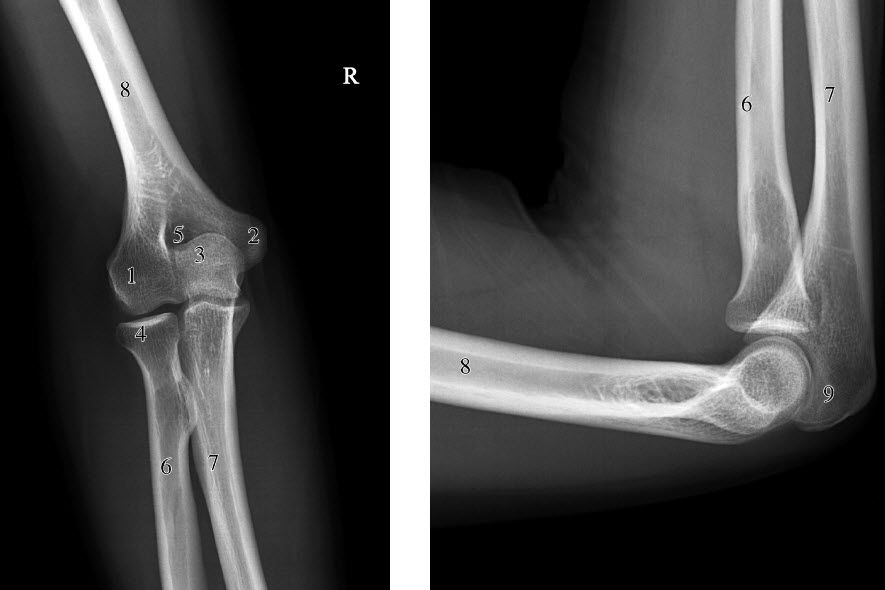
\includegraphics[width=6.73958in,height=3.32292in]{./images/Image00004.jpg}
\end{table}

\begin{table}[htbp]
\centering
\caption{引起昏迷的全身性疾病及其分类、发病机制和常见病因}
\label{tab2-2}
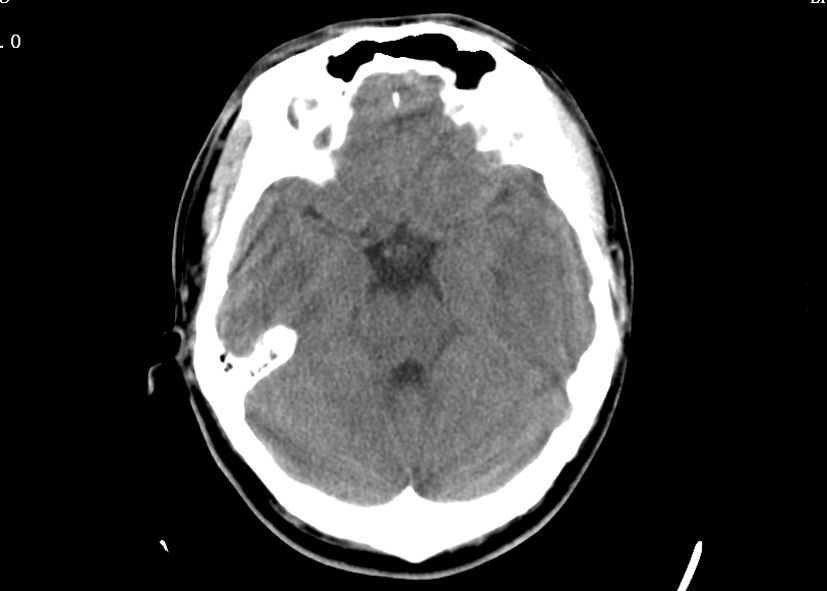
\includegraphics[width=6.73958in,height=4.83333in]{./images/Image00005.jpg}
\end{table}

\subparagraph{脉搏}

脉搏触诊有助于及时发现急性心源性脑缺血综合征。脉慢而洪大见于脑出血、酒精中毒;脑脓肿患者的脉搏常缓慢、充实而规则;而脑膜炎患者的脉搏多细速。颠茄类、氯丙嗪中毒时脉搏显著增快。脉搏先慢后快,同时伴有血压下降者,可见于脑疝压迫脑干、延髓生命中枢衰竭,提示预后不良。

\subparagraph{呼吸}

观察患者的呼吸方式、节律和频率等。呼吸深而快,常见于代谢性酸中毒(糖尿病、尿毒症等);鼾声呼吸且伴有呼吸时一侧面肌瘫痪者提示脑出血。浅而快速的规律性呼吸见于休克、心肺疾患或镇静催眠药中毒引起的呼吸衰竭,肺炎等缺氧性疾病可伴发绀和鼻翼扇动;呼吸深而慢、同时脉搏慢而有力和血压增高,为颅内压增高的表现。呼吸过慢并伴有叹息样呼吸常为吗啡类药物中毒。呼气带有氨味见于尿毒症昏迷;带有苹果味见于糖尿病昏迷;苦杏仁气味提示氢氰酸(苦杏仁、木薯、氰化物等)中毒;呈酒味提示酒精中毒;呼气及排泄物有大蒜样臭味可见于有机磷农药中毒;呼气中及尿液出现“肝臭”者提示肝性脑病。

昏迷患者呼吸节律的异常类型常常提示脑部病变的部位,与神经功能障碍水平定位有密切关系。双侧额叶损害可出现过度换气后呼吸暂停(PHVA)现象,即每在5~10次深呼吸后呼吸暂停。脑部广泛病损使中脑内呼吸中枢失去大脑的控制时,可出现潮式呼吸,即陈-施呼吸(Cheyne-Stokes
respiration,CSR),表现为呼吸由浅慢逐渐变为深快,再由深快变为浅慢,随后出现一段呼吸暂停后,然后重复上述周期性呼吸。潮式呼吸的周期可以长达30秒~2分钟,暂停时间可长达5~30秒。当中脑和脑桥上部功能受损后,可出现中枢神经源性过度呼吸(central
neurogenic
hyperventilation,CNH),呼吸深、快、均匀、持久,频率达40~70次/分。脑桥下部损害后可出现:①喘息样呼吸(gasping
of
breaths),常在濒死时出现,表现为深呼吸、较慢的频率,跳跃式深吸气,呼吸暂停6~10秒,可见于延髓内肿瘤或严重的药物中毒时;②交替呼吸,表现为一次强呼吸和一次弱呼吸交替;③间歇(Biot)呼吸,表现为每3~4次呼吸后出现呼吸暂停;④长吸式呼吸(apneustic
breathing),是一种吸气持续的延长性吸气痉挛,吸2~3次呼1次或吸足气后呼吸暂停。所谓鱼嘴式呼吸(每次吸气时下颌张开似鱼嘴),亦见于脑干下部损害时,常为预后严重的征兆。延髓受损时,呼吸紊乱更为严重,频率和幅度均不时改变,间以不规则地呼吸中断,有人亦称其为“共济失调性呼吸”(ataxic
breathing),最后发展至呼吸完全停止。在天幕上占位病变发展至出现天幕裂孔疝和枕大孔疝的过程中,有时可见到呼吸形式的一系列改变(潮式呼吸→中枢神经源性过度呼吸→喘息式呼吸→共济失调性呼吸),提示脑干功能自首端向尾端逐渐发生障碍。

\subparagraph{血压}

血压显著增高,见于脑出血、高血压脑病、颅内压增高等;血压过低常见于糖尿病昏迷、酒精中毒、巴比妥类药物中毒等。

\subparagraph{皮肤黏膜}

皮肤灼热干燥见于中暑高热;皮肤湿润多汗见于低血糖昏迷、有机磷农药中毒等;皮肤苍白常见于尿毒症性、低血糖性昏迷等;皮肤潮红见于脑出血、颠茄类中毒及酒精中毒;口唇发绀为严重缺氧如窒息、自缢或肺性脑病等;口唇樱红考虑一氧化碳中毒、严重酸中毒;口角见到单纯疱疹,考虑为疱疹性脑炎、脑型疟疾、大叶性肺炎或流脑等;皮肤巩膜黄染应考虑肝性脑病或药物中毒;昏迷伴有结合膜瘀斑、皮疹、皮肤瘀斑,须鉴别脓毒症、流脑、流行性出血热等引起的昏迷;有无头部、颜面部皮肤损伤的痕迹,有无舌咬伤、耳鼻部出血、脑脊液漏、耳后及皮下出血等,对诊断颅骨骨折、颅脑外伤及癫痫大发作常有帮助;颈部手术瘢痕可能提示甲状腺或甲状旁腺疾患,电解质不平衡或内分泌功能障碍;胸腔手术或乳房手术瘢痕应想到颅内转移或伴随于恶性肿瘤的高钙血症、低钠血症等电解质紊乱。应注意肢体、皮肤上成串的针疤或皮下脓肿可能曾滥用药物。

\hypertarget{text00010.htmlux5cux23CHP1-2-2-1-3}{}
(三) 神经系统检查

意识障碍时神经系统查体主要包括以下几个方面的检查
:眼征、对疼痛刺激的反应、瘫痪体征、脑干反射、锥体束征和脑膜刺激征等。

\subparagraph{眼征}

包括以下几个方面:

\hypertarget{text00010.htmlux5cux23CHP1-2-2-1-3-1-1}{}
(1) 瞳孔变化:

观察瞳孔的大小、形状、位置、双侧对称性及对光反应,可帮助判断神经损害的部位及程度。①瞳孔对光反射:为光线刺激瞳孔引起的缩瞳反射。其传导径路为:视网膜→视神经→中脑被盖前区→埃-魏核→动眼神经→膝状神经节→颈上交感神经节节后纤维→瞳孔括约肌,径路上任何一处损害均可引起对光反射丧失和瞳孔散大。瞳孔对光反射与昏迷程度成正比(但巴比妥类中毒虽呈深昏迷,对光反射却残存是特征)。②瞳孔改变与病因:单侧瞳孔扩大,除外药物作用,昏迷患者单侧瞳孔扩大(≥5mm)者,可定为视神经损害或动眼神经损害造成。视神经损害常由于急性颅脑外伤伴发视神经损伤,有球后视神经炎过去史,或局部肿瘤或动脉瘤压迫引起单侧性黑矇性瞳孔麻痹,同侧直接光反射及对侧间接光反射消失;视神经萎缩者,亦可见该侧瞳孔扩大。动眼神经损害单侧瞳孔扩大,多见于后交通动脉瘤破裂引起的蛛网膜下腔出血,也可见于颞叶钩回疝、颅脑外伤伴发硬膜外血肿、脑出血、脑肿瘤等压迫。颈内动脉血栓形成,大脑中动脉浅支或深支梗塞时,亦可见单侧瞳孔扩大。个别癫痫患者抽搐后出现暂时性单侧瞳孔扩大,机制不明。双侧瞳孔扩大,可见于药物或食物中毒如颠茄类、巴比妥类(有时缩小)、氰化物、肉毒杆菌中毒等;脑疝进行到晚期瞳孔由单侧扩大扩展为双侧扩大,昏迷加深,提示预后不良。天幕上病变尚未引起脑疝或中脑结构移位时,瞳孔大小接近正常,若发生小脑幕切迹疝,则见病灶侧瞳孔扩大,对光反射消失,若观察脑疝形成的全过程,则可发现扩大侧瞳孔先有缩小的改变(由于动眼神经的压迫与牵拉,病侧缩瞳纤维首先受到刺激,继而麻痹)。单侧瞳孔缩小较少见,上述幕上占位病变导致早期颞叶钩回疝时,可见同侧瞳孔缩小,而光反射存在;脑干梗死也可见到一侧瞳孔缩小(霍纳综合征表现之一)。双侧瞳孔缩小,可见于氯丙嗪、吗啡类药物、有机磷农药、水合氯醛、毒蕈等中毒与尿毒症;双侧瞳孔缩小如针眼,伴有高热是原发性脑桥出血的特征,若患者还有四肢阵发性强直性抽搐则是脑室出血的表现。中央型间脑疝而致双侧下丘脑损害可出现双侧瞳孔缩小。

\hypertarget{text00010.htmlux5cux23CHP1-2-2-1-3-1-2}{}
(2) 眼球运动:

眼球运动受大脑皮质、脑桥、中脑和第3、4、6脑神经控制,其运动异常有重要的定位意义。在代谢性脑病中,仅巴比妥类和苯妥英钠中毒可有眼球运动障碍。若患者的眼球和浅睡眠一样,能缓慢地向两侧转动,说明脑桥和中脑的有关功能尚相对地完好,据此可推测天幕下病变引起的昏迷可能性较小。一侧大脑半球有较广泛的损害时,患者双眼常偏向瘫痪肢体的对侧;一侧脑桥受损时,则双眼偏向肢体瘫痪的同侧。在双侧大脑皮质急性病变时,可见到有眼球激动现象,每隔几秒钟双眼出现强烈的快速摆动。丘脑底部和上位中脑损害患者,眼球可能向下和向内转,就像盯着自己鼻尖看。眼球浮动(ocular
bobbing)是双眼球快速同向下转后又缓慢地向上转恢复至原位,每分钟重复2~3次,转动的幅度约1~3mm,它发生于眼球水平向运动机制被破坏的情况,其机制为脑桥侧视中枢受损,而中脑的眼球垂直运动中枢未受损之故,见于脑桥的双侧性损害。脑干广泛严重损害时,眼球运动完全丧失而固定在正中位。垂直性眼球运动障碍如双眼向上或向下凝视,提示中脑四叠体附近或下丘脑病变;分离性眼球运动可为小脑损害表现。

\hypertarget{text00010.htmlux5cux23CHP1-2-2-1-3-1-3}{}
(3) 眼底检查:

凡是能引起颅内压增高的疾病均可引起眼底改变。颅脑外伤或颅内出血后12~24小时即可出现视神经乳头水肿的变化;但严重的视乳头水肿多数是由于长期颅内压增高的后果,应考虑有脑肿瘤、脑脓肿等占位病变的可能。如视网膜有广泛的渗出物、出血,则应考虑有糖尿病、尿毒症、高血压脑病等可能。玻璃体下较大的或视网膜广泛的浅表出血通常见于蛛网膜下腔出血。

\subparagraph{对疼痛刺激的反应}

用力按压眶上缘、胸骨检查昏迷患者对疼痛的运动反应,有助于定位脑功能障碍水平或判断昏迷的程度。出现单侧或不对称性姿势反应时,健侧上肢可见防御反应,病侧则无,提示瘫痪对侧大脑半球或脑干病变。观察面部疼痛表情时,可根据面肌运动,判断有无面瘫。疼痛引起去皮质强直(decorticate
rigidity),表现为上肢内收和屈曲,下肢伸直,与丘脑或大脑半球病变有关;去脑强直(decerebrate
rigidity)表现为四肢伸直,肌张力增高或角弓反张,提示中脑功能受损,较去皮质强直脑功能障碍程度更为严重。脑桥和延髓病变患者通常对疼痛无反应,偶可发现膝部屈曲(脊髓反射)。

\subparagraph{瘫痪体征}

意识障碍和昏迷患者的瘫痪检查,可通过疼痛刺激观察面部表情与肢体活动,以及肢体坠落试验等来判定。①观察面颊:一侧面瘫时,可见该侧鼻唇沟变浅,口角低垂,睑裂增宽,呼气时面颊鼓起,吸气时面颊塌陷,呈吸烟斗动作。②疼痛刺激:压迫眶上切迹或捏掐肢体,观察患者肢体活动情况,瘫痪侧少动或不动。③观察双眼球共同偏视(见前述)。④胸骨反射:针刺胸骨柄部,引起一侧或双侧上肢的屈曲反应,手移向胸骨部,刺激加重,可波及下肢。一侧肢体反射消失或运动反应弱,提示该侧肢体瘫痪。⑤上肢坠落试验:将患者双上肢抬起,使与躯干呈垂直位,突然放手,观察肢体坠落情况,瘫痪肢体迅速坠落而且沉重,无瘫痪肢体则向外侧倾倒,缓慢坠落。⑥下肢坠落试验:将患者下肢膝部屈曲抬高,足跟着床,突然松手时,瘫痪侧肢体不能自动伸直,并向外侧倾倒;无瘫痪肢体则呈弹跳式伸直,并能保持足垂直位。⑦足外旋试验:先将患者的双下肢伸直放平,然后把双足扶直并拢,突然松开时,则瘫痪肢体的足立刻外旋倾倒,足外缘着床;无瘫痪的足,仍能维持足垂直位。⑧反射的改变:瘫痪肢体侧常伴有中枢性面瘫,腹壁、提睾反射减弱或消失,腱反射增强,病理反射阳性。

\subparagraph{脑干反射}

可通过睫脊反射(ciliospinal reflex)、角膜反射(corneal
reflex)、头眼反射(oculocephalic reflex)和眼前庭反射(oculovestibular
reflex)等脑干反射来判断是否存在脑干功能损害。反射性眼球运动包括头眼反射和眼前庭反射。

\hypertarget{text00010.htmlux5cux23CHP1-2-2-1-3-4-1}{}
(1) 睫脊反射:

给予颈部皮肤疼痛刺激时可引起双侧瞳孔散大,此反射存在提示下位脑干、颈髓、上胸段脊髓及颈交感神经功能正常。

\hypertarget{text00010.htmlux5cux23CHP1-2-2-1-3-4-2}{}
(2) 角膜反射:

角膜反射是由三叉神经的眼神经与面神经共同完成的,当三叉神经的第一支(眼神经)或面神经损害时,均可出现角膜反射消失。若脑桥上部和中脑未受累及,角膜反射存在;一侧角膜反射消失见于同侧面神经病变(同侧脑桥),双角膜反射消失见于一侧三叉神经受损或双侧面神经受损,提示中脑或脑桥受累,常有意识障碍。

\hypertarget{text00010.htmlux5cux23CHP1-2-2-1-3-4-3}{}
(3) 头眼反射:

又称玩偶眼试验(Doll's eye
test)。在浅昏迷患者,检查者使其眼睑睁开,并将患者的头向两侧或前后转动,先慢后快,患者双眼反射地朝与头转动相反的方向转动(如头转向右侧时,双眼凝视偏向左侧),谓之头眼反射(本体觉转头反射、环偶眼现象)阳性。在婴儿为正常反射,随着大脑发育而抑制。头眼反射的刺激主要通过颈部肌肉本体觉,通过本体觉神经纤维进入脊髓,先经过颈髓2~4节段的背根,然后进入颈髓再上升达到延髓前庭神经核、中脑顶盖部、脑桥,以及第3、4、6脑神经。正常人清醒状态下,头眼反射为大脑半球发起的视觉固定(或注视,visual
fixation)所抑制,故正常人头眼反射不存在。在嗜睡患者,开始2或3次转头可能引起相反的同向眼动,以后由于转头动作通常使患者觉醒而头眼反射消失。此反射在大脑半球弥漫性病变和间脑病变所致昏迷时出现并加强;脑干病变时此反射消失,如一侧脑干病变,头向该侧转动时无反射,向对侧仍存在。应强调的是:在怀疑有颈椎脱位与骨折可能的患者,绝对禁忌作此项检查。

\hypertarget{text00010.htmlux5cux23CHP1-2-2-1-3-4-4}{}
(4) 眼前庭反射:

或称冷热水试验。用注射器向一侧外耳道注入1ml冰水,大脑半球弥漫性病变而脑干功能正常时,出现双眼向冰水灌注侧强直性同向运动;昏迷患者,如存在完全的反射性眼球运动,提示脑桥至中脑水平的脑干功能完好;中脑病变时,眼前庭检查可显示灌注对侧眼球内收不能,同侧眼外展正常;脑桥病变时反应完全丧失。

\subparagraph{脑膜刺激征}

脑膜刺激征包括颈强直(简称颈强)、Kernig征(凯尔尼格征)和Brudzinski征(布鲁津斯基征)等。颈上节段的脊神经根受刺激引起颈强直,腰骶节段的脊神经根受刺激,则出现Kernig征和Brudzinski征。阳性提示有脑膜炎、蛛网膜下腔出血、脑炎、脑水肿及颅内压增高等的可能。深昏迷时脑膜刺激征可消失。检查方法包括:

\hypertarget{text00010.htmlux5cux23CHP1-2-2-1-3-5-1}{}
(1) 屈颈试验:

患者仰卧,检查者托患者枕部并使其头部前屈而表现不同程度的颈强,被动屈颈受限,称为颈强直,但需排除颈椎病。正常人屈颈时下颏可触及胸骨柄,部分老年人及肥胖者除外。

\hypertarget{text00010.htmlux5cux23CHP1-2-2-1-3-5-2}{}
(2) Kernig征:

患者仰卧,下肢于髋、膝关节处屈曲成直角,检查者于膝关节处试行伸直小腿,如伸直受限并出现疼痛,大、小腿间夹角<
135°,为Kernig征阳性。如颈强(+)而Kernig征(−),称为颈强-Kernig征分离,见于后颅窝占位性病变和小脑扁桃体疝等。

\hypertarget{text00010.htmlux5cux23CHP1-2-2-1-3-5-3}{}
(3) Brudzinski征:

患者仰卧屈颈时出现双侧髋、膝部屈曲;一侧下肢膝关节屈曲位,检查者使该侧下肢向腹部屈曲,对侧下肢亦发生屈曲(下肢征),均为Brudzinski征阳性。

\subparagraph{反射检查}

一般认为,浅反射由减退至消失而同时深反射由亢进至消失,均提示昏迷的程度加深。常用的深反射(为肌腱和关节反射)有肱二头肌、肱三头肌反射,桡骨膜反射,膝反射,跟腱反射等;常用的浅反射(浅反射是刺激皮肤、黏膜、角膜等引起肌肉快速收缩反应)有角膜反射、咽反射、腹壁反射、提睾反射、跖反射、肛门反射等。常用的病理反射有:

\hypertarget{text00010.htmlux5cux23CHP1-2-2-1-3-6-1}{}
(1) 巴宾斯基征(Babinski征):

是经典的病理反射,提示锥体束受损。用竹签轻划足底外侧,自足跟向前至小趾根部足掌时转向内侧,阳性反应为趾背屈,可伴其他足趾扇形展开。

\hypertarget{text00010.htmlux5cux23CHP1-2-2-1-3-6-2}{}
(2) 巴宾斯基等位征:

包括:①Chaddock征:由外踝下方向前划至足背外侧;②Oppenheim征:用拇指和示指沿胫骨前缘自上而下用力下滑;③Schaeffer征:用手挤压跟腱;④Gordon征:用手挤压腓肠肌;⑤Gonda征:用力下压第4、5足趾,数分钟后突然放松;⑥Pussep征:轻划足背外侧缘。阳性反应均为趾背屈。临床意义一般认为同Babinski征。

\hypertarget{text00010.htmlux5cux23CHP1-2-2-1-3-6-3}{}
(3) 强握反射:

指检查者用手指触摸患者手掌时被强直性握住的一种反射。新生儿为正常反射,成人见于对侧额叶运动前区病变。

\hypertarget{text00010.htmlux5cux23CHP1-2-2-1-3-6-4}{}
(4) 脊髓自主反射:

脊髓横贯性病变时,针刺病变平面以下皮肤引起单侧或双侧髋、膝、踝部屈曲(三短反射)和Babinski征阳性。若双侧屈曲并伴腹肌收缩、膀胱及直肠排空,以及病变以下竖毛、出汗、皮肤发红等,称为总体反射。

对于昏迷患者除重点注意以上项目外,尚应注意胸、腹部体征如昏迷偏瘫患者伴有心脏杂音,心房纤颤,考虑心脏病伴有脑梗死;昏迷、抽搐伴有心音片刻听不到,考虑阿-斯综合征;昏迷、休克、肺部啰音等,考虑中毒性肺炎;昏迷患者伴腹水、肝脾大或缩小,常提示肝性脑病、血液病、细菌性心内膜炎、脓毒症等可能性。

实验室检查与特殊检查应根据需要选择进行,但除三大常规外,对于意识障碍和昏迷患者,血清电解质、尿素氮(BUN)、CO\textsubscript{2}
CP、血糖等应列为常规检查;对病情不允许者必须先就地抢救,视病情许可后再进行补充。脑电图、头颅CT和MRI,以及脑脊液检查对昏迷的病因鉴别有重要意义。

在通过上述病史询问,体检,神经系统检查及必要的有关辅助检查后,一般可依下列顺序对意识障碍与昏迷进行诊断和鉴别诊断。

\subsubsection{判断是否为意识障碍和昏迷}

临床上判断是否属于意识障碍和昏迷一般不难,但首先应排除下述两种情况:

\subparagraph{几种特殊类型的意识障碍}

\hypertarget{text00010.htmlux5cux23CHP1-2-2-2-1-1}{}
(1) 去皮质综合征(decorticate syndrome):

也称去大脑皮质状态(apallic
state),是由于双侧大脑皮质发生弥散性的严重损害而导致大脑皮质功能减退或丧失,皮质下功能仍保存。其特点是皮质与脑干的功能出现分离现象:大脑皮质功能丧失,对外界刺激无任何意识反应,不言不语;而脑干各部分的功能正常:患者眼睑开闭自如,常睁眼凝视(即醒状昏迷),痛觉灵敏(对疼痛刺激有痛苦表情及逃避反应),角膜与瞳孔对光反射均正常。四肢肌张力增高,双上肢常屈曲,双下肢伸直(去皮质强直),大小便失禁,还可出现吸吮反射及强握反射,甚至伴有手足徐动、震颤、舞蹈样运动等不随意运动。该综合征常见于缺氧性脑病、脑炎、中毒和严重颅脑外伤等。

\hypertarget{text00010.htmlux5cux23CHP1-2-2-2-1-2}{}
(2) 无动性缄默症(akinetic mutism):

又称睁眼昏迷(coma
vigil),由脑干上部和丘脑的ARAS受损引起,此时大脑半球及其传出通路无病变。患者能注视周围环境及人物,貌似清醒,但不能活动或言语,二便失禁。肌张力减低,无锥体束征。强烈刺激不能改变其意识状态,存在觉醒-睡眠周期。本症常见于脑干梗死。

\hypertarget{text00010.htmlux5cux23CHP1-2-2-2-1-3}{}
(3) 植物状态(vegetative state):

是指大脑半球严重受损而脑干功能相对保留的一种状态。表现为对自身和外界的认知功能完全丧失,能睁眼,有睡眠和觉醒周期,可有无意义哭笑,二便失禁。肢体可有无意识的随意运动,脑干反射存在。持续性植物状态指颅脑外伤后植物状态持续12个月以上,其他原因持续3个月以上。

\subparagraph{神经精神疾病所致的几种貌似昏迷状态}

\hypertarget{text00010.htmlux5cux23CHP1-2-2-2-2-1}{}
(1) 精神抑制状态(depression state):

常见于强烈精神刺激后或癔症性昏睡发作,患者表现出僵卧不语,对外界刺激如呼唤、推摇,甚至疼痛刺激常不发生反应。双目紧闭,扳开眼睑时有明显抵抗感,并见眼球向上翻动,放开后双眼迅速紧闭。瞳孔大小正常,光反应灵敏,眼脑反射正常,无病理反射。脑电图呈觉醒反应,经适当治疗可迅速复常。癔症性昏睡,多数尚有呼吸急促,也有屏气变慢,检查四肢肌张力增高,对被动活动多有抵抗,有时四肢伸直、屈曲或挣扎、乱动。常呈阵发性,多属一过性病程,在暗示治疗后可迅速恢复。

\hypertarget{text00010.htmlux5cux23CHP1-2-2-2-2-2}{}
(2) 木僵(stupor):

表现为不语不动,不饮不食,对外界刺激缺乏反应,甚至出现大小便潴留,多伴有蜡样屈曲和违拗症,言语刺激触及其痛处时可有流泪、心率增快等情感反应,缓解后多能清楚回忆发病过程。见于精神分裂症的紧张性木僵、严重抑郁症的抑郁性木僵、反应性精神障碍的反应性木僵等。

\hypertarget{text00010.htmlux5cux23CHP1-2-2-2-2-3}{}
(3) 闭锁综合征(locked-in syndrome):

又称去传出状态(deefferented
state)。病变位于脑桥基底部,双侧锥体束和皮质脑干束均受累。患者意识清醒,因运动传出通路几乎完全受损而呈失运动状态,除尚有部分眼球运动外,呈现四肢瘫,不能说话和吞咽,表情缺乏,就像全身被闭锁,但可理解语言和动作,能以睁闭或眼垂直运动示意。当临床怀疑本症时,可让患者“睁开你的眼睛”、“向上看”、“向下看”和“看你的鼻尖”等,可作出鉴别。

\hypertarget{text00010.htmlux5cux23CHP1-2-2-2-2-4}{}
(4) 意志缺乏症(abulia):

患者处于清醒状态,运动感觉功能存在,但因缺乏始动性而不语不动,对刺激无反应,无欲望,呈严重淡漠状态,可有额叶释放反射,如掌颏反射、吸吮反射等。本症多由双侧额叶病变所致。

\hypertarget{text00010.htmlux5cux23CHP1-2-2-2-2-5}{}
(5) 失语(aphasia):

程度较重的失语患者,特别是伴有嗜睡、瘫痪时,对外界刺激失去反应能力而易被误认为昏迷。如系失语而非昏迷的患者,对声、光、疼痛刺激的反应是灵敏的;对言语以外的示意性动作、表情等仍能领会、理解,而有适当的表情反应,或喃喃发声,欲语不能。

\subsubsection{意识障碍和昏迷程度的评定}

临床上除将意识障碍分为嗜睡、昏睡、浅昏迷、中昏迷和深昏迷五级(见前述)外,常用格拉斯哥昏迷计分法(Glasgow
coma
scale,GCS)。GCS是以睁眼(觉醒水平)、言语(意识内容)和运动反应(病损平面)三项指标的15项检查结果来判断患者昏迷和意识障碍的程度,见表\ref{tab2-3}。以上三项检查共计15分。GCS分值愈低,脑损害的程度愈重,预后亦愈差。但此量表有一定局限性:对眼肌麻痹、眼睑肿胀者不能评价其睁眼反应,对气管插管或切开者不能评价其言语活动,四肢瘫患者不能评价其运动反应。1978年此量表被修订为Glasgow-Pittsburgh量表,增加了对光反射、脑干反射、抽搐情况和自发性呼吸四大类检查,见表\ref{tab2-4}。合计为7项35级,最高为35分,最低为7分。在颅脑损伤中,35~28分为轻型,27~21分为中型,20~15分为重型,14~7分为特重型颅脑损伤。该观察表即可判定昏迷程度,也反映了脑功能受损水平。

\subsubsection{意识障碍和昏迷的病因诊断}

意识障碍和昏迷的病因诊断极其重要。通常必须依据病史、体格和神经系统检查,以及有关的辅助检查资料,经过综合分析,能查出导致昏迷的原发病因。由于昏迷的病因众多,而且某些病例的病程进展甚快,病情危重或因条件所限,无法进行详细或特殊的辅助检查,使病因诊断受到影响。但以下诊断思路具有较大的临床价值。

\hypertarget{text00010.htmlux5cux23CHP1-2-2-4-1}{}
(一) 确定是颅内疾病抑或全身性疾病

通常先确定是颅内疾病抑或全身性疾病
,如确定意识障碍和昏迷是颅内病变引起,尚需进一步确定是颅内局限性病变抑或弥散性病变,如是前者,它是位于幕上抑或幕下,具体病因是什么。

\subparagraph{颅内疾病}

位于颅内的原发性病变,在临床上通常先有大脑或脑干受损的定位症状和体征,较早出现意识障碍和精神症状,伴明显的颅内高压症和脑膜刺激征,提示颅内病变的有关辅助检查如脑脊液检查、CT扫描等常有阳性发现。临床上可根据神经系统体征基本上将表现分为两类:①主要呈现局限性神经体征,如脑神经损害、肢体瘫痪、局限性抽搐、偏侧锥体束征等,常见于脑出血、梗死、脑炎、外伤、占位性病变等;②主要表现为脑膜刺激征而无局限性神经体征,最多见于脑膜炎、蛛网膜下腔出血等。

\begin{table}[htbp]
\centering
\caption{GCS昏迷评定量表}
\label{tab2-3}
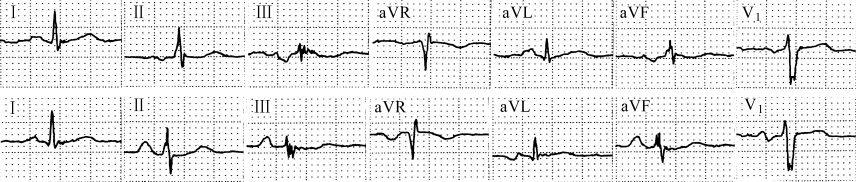
\includegraphics[width=6.66667in,height=2.03125in]{./images/Image00006.jpg}
\end{table}

\begin{table}[htbp]
\centering
\caption{Glasgow-Pittsburgh昏迷观察表}
\label{tab2-4}
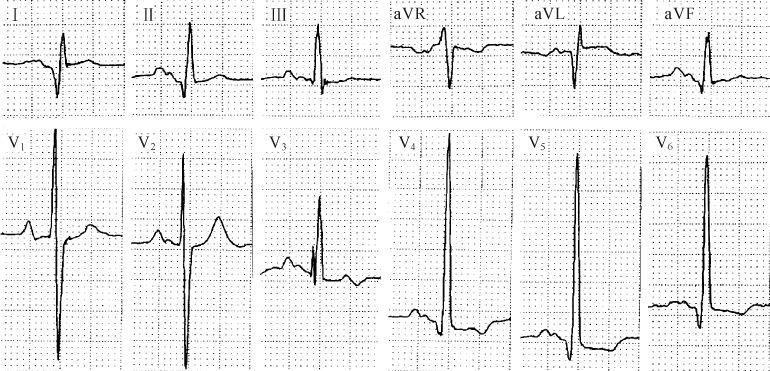
\includegraphics[width=6.69792in,height=4.21875in]{./images/Image00007.jpg}
\end{table}

如确定昏迷是颅内病变引起,尚可将颅内病变又进一步区分为颅内幕上局限性病变、幕下局限性病变和颅内弥散性病变三组。它们的特征参见表\ref{tab2-1}。

\subparagraph{全身性疾病}

全身性疾病可影响脑代谢而引起弥散性脑损害,又称代谢性脑病。同原发性颅内病变相比,其临床特点为:先有颅外器官原发病的症状和体征,以及相应的实验室检查阳性发现,后才出现脑部受损的征象。由于脑部损害为非特异性或仅是弥散性功能抑制,临床上一般无持久性和明显的局限性神经体征和脑膜刺激征,主要是多灶性神经功能缺乏的症状和体征,且大都较对称;通常先有精神异常,意识内容减少。一般是注意力减退,记忆和定向障碍,计算和判断力降低,尚有错觉、幻觉,随病程进展,意识障碍加深。此后有的可出现不同层次结构损害的神经体征,如昏迷较深和代谢性呼吸抑制很严重,而眼球运动和瞳孔受累却相对较轻。脑脊液改变不显著,颅脑CT扫描等检查无特殊改变,不能发现定位病灶。其病因很多,它们的特征参见表\ref{tab2-2}。

\hypertarget{text00010.htmlux5cux23CHP1-2-2-4-2}{}
(二) 根据患者是否伴有脑膜刺激征和脑局灶体征来判断昏迷的病因

\subparagraph{脑膜刺激征(+)而脑局灶性体征(−)}

\hypertarget{text00010.htmlux5cux23CHP1-2-2-4-2-1-1}{}
(1) 突发剧烈头痛:

蛛网膜下腔出血(脑动脉瘤、脑动静脉畸形破裂)。

\hypertarget{text00010.htmlux5cux23CHP1-2-2-4-2-1-2}{}
(2) 急性发病、发热在先:

化脓性脑膜炎、乙型脑炎、其他急性脑炎等。

\hypertarget{text00010.htmlux5cux23CHP1-2-2-4-2-1-3}{}
(3) 亚急性或慢性发病:

真菌性、结核性、癌性脑膜炎。

\subparagraph{脑膜刺激征(−)而脑局灶性体征(+)}

\hypertarget{text00010.htmlux5cux23CHP1-2-2-4-2-2-1}{}
(1) 突然起病者:

如脑出血、脑栓塞、脑梗死等。

\hypertarget{text00010.htmlux5cux23CHP1-2-2-4-2-2-2}{}
(2) 以发热为前驱症状:

如脑脓肿、血栓性静脉炎、各种脑炎、急性播散性脑脊髓炎、急性出血性白质脑病等。

\hypertarget{text00010.htmlux5cux23CHP1-2-2-4-2-2-3}{}
(3) 与外伤有关:

如脑挫伤、硬膜外血肿、硬膜下血肿等。

\hypertarget{text00010.htmlux5cux23CHP1-2-2-4-2-2-4}{}
(4) 缓慢起病、颅内压增高者:

脑肿瘤、慢性硬膜下血肿、脑寄生虫病等。

\subparagraph{脑膜刺激征(−)和脑局灶性体征(−)}

\hypertarget{text00010.htmlux5cux23CHP1-2-2-4-2-3-1}{}
(1) 有明确中毒原因:

如酒精、麻醉药、安眠药、一氧化碳中毒等。

\hypertarget{text00010.htmlux5cux23CHP1-2-2-4-2-3-2}{}
(2) 尿检异常:

尿毒症、糖尿病、急性尿卟啉症等。

\hypertarget{text00010.htmlux5cux23CHP1-2-2-4-2-3-3}{}
(3) 休克状态:

低血糖、心肌梗死、肺栓塞、大出血等。

\hypertarget{text00010.htmlux5cux23CHP1-2-2-4-2-3-4}{}
(4) 有黄疸:

肝性脑病等。

\hypertarget{text00010.htmlux5cux23CHP1-2-2-4-2-3-5}{}
(5) 有发绀:

肺性脑病等。

\hypertarget{text00010.htmlux5cux23CHP1-2-2-4-2-3-6}{}
(6) 有高热:

重症感染、中暑、甲状腺危象等。

\hypertarget{text00010.htmlux5cux23CHP1-2-2-4-2-3-7}{}
(7) 体温过低:

休克、酒精中毒、黏液性水肿昏迷等。

\hypertarget{text00010.htmlux5cux23CHP1-2-2-4-2-3-8}{}
(8) 头部外伤:

脑震荡等。

\hypertarget{text00010.htmlux5cux23CHP1-2-2-4-2-3-9}{}
(9) 其他:

癫痫等。

\subsection{处理原则}

\subparagraph{昏迷的最初处理}

常规措施有:①保持呼吸道通畅,氧疗,必要时气管插管或切开行人工呼吸。②维持循环功能,尽早开放静脉,建立输液通路(1~3个)。有休克应迅速扩充血容量,使用血管活性药物,尽快使收缩血压稳定在100mmHg左右。有心律失常者应予以纠正;有心肌收缩力减弱者应给予强心剂;心跳骤停时应立即行心肺复苏。③纳洛酮:常用剂量每次0.4~0.8mg,静脉注射或肌注,无反应可隔10~15分钟重复用药,直达预期效果;亦可用1.2~2.0mg加入250~500ml液体中静滴。

\subparagraph{病因治疗}

针对病因采取及时果断措施是抢救成功的关键。若昏迷的病因已明确,则应迅速给予有效病因治疗。如由颅内占位性病变引起者,若条件许可应尽早作开颅手术,摘除肿瘤;细菌性脑膜脑炎引起者,应迅速给予大量而有效的抗生素治疗;因脑型疟疾而引起的昏迷,则可给盐酸奎宁0.5g置于5\%葡萄糖液250~500ml中静滴;由于低血糖引起者应立即给予高渗葡萄糖液;若为有机磷农药中毒所致者,应立即用胆碱酯酶复能剂和阿托品等特效解毒剂;糖尿病昏迷应予胰岛素治疗等。

\subparagraph{对症支持疗法}

包括控制脑水肿、降低颅内压,维持水电解质平衡,镇静止痛,防治各种并发症(如急性心力衰竭、急性呼吸衰竭、消化道出血、急性肾功能衰竭、急性脑功能衰竭等)等,详见有关章节。

\protect\hypertarget{text00011.html}{}{}

\hypertarget{text00011.htmlux5cux23CHP1-2-4}{}
参 考 文 献

1. 张文武.急诊内科学.第2版.北京:人民卫生出版社,2007

2. 贾建平.神经病学.第6版.北京:人民卫生出版社,2008

3. Rowland LP. Merritt's Neurology. 11th ed. New York:Lippincott
Williams & Wilkins,2005

\protect\hypertarget{text00012.html}{}{}

\chapter{眩 晕}

眩晕是一主观症状,是机体对于空间关系的定向感觉障碍或平衡感觉障碍,是一种运动错觉,患者感外境或自身在旋转、移动或摇晃。在眩晕症状出现的同时,常伴有平衡失调、站立不稳、眼球震颤、指物偏向、恶心、呕吐、面色苍白、出汗及心率和血压的改变。

临床上可将眩晕分为前庭系统性眩晕(亦称真性眩晕)及非前庭系统性眩晕(亦称头晕)。前者由前庭神经系统病变(包括前庭末梢器、前庭神经及前庭的中枢连接)所引起,为真性眩晕,表现为有运动错觉的眩晕,例如自觉旋转、摇晃、移动感;后者常为头昏(头重脚轻、眼花、头脑昏昏沉沉、颅内在转动等诉说),但并无外境或自身旋转的运动觉,常由心血管系统疾病,全身中毒性、代谢性疾病,贫血,眼病等疾患所引起。

\subsection{病因与发病机制}

\subsubsection{病因分类}

眩晕的病因分类有多种方法,各家不甚统一,各有其优缺点。笔者认为根据神经系统疾病的诊断步骤先定位再定性的方法,较为实用,即根据病变的解剖部位及结合病因予以分类。现将常见的疾病列举如下:

\hypertarget{text00012.htmlux5cux23CHP1-3-1-1-1}{}
(一) 前庭系统性眩晕

包括前庭末梢感受器
、前庭神经、前庭诸核、内侧纵束、小脑、前庭皮质代表区之各种病损所产生的真性眩晕。

\subparagraph{耳源性}

例如外耳道耵聍,急、慢性中耳炎,咽鼓管阻塞,鼓膜内陷,耳硬化症,迷路炎,慢性中耳炎内耳并发症(瘘管形成),梅尼埃病(Meniere
disease),运动病,良性位置性眩晕,迷路动脉血供障碍,内耳震荡等。

\subparagraph{前庭神经病损}

前庭神经元炎、听神经鞘膜瘤、脑桥小角其他肿瘤、前庭神经炎、前庭神经外伤(岩锥骨折)或中毒性损害。

\subparagraph{脑干病变}

脑桥、延髓的血管性和肿瘤性病变、脑干脑炎、多发性硬化、延髓空洞症、第四脑室肿瘤及囊肿。

\subparagraph{小脑病变}

肿瘤、脓肿、出血及损伤。

\subparagraph{大脑病变}

颞叶肿瘤或血管性病变,颞叶癫痫。

\subparagraph{颈椎病变}

颈椎肥大性改变及颈椎间盘突出。

\hypertarget{text00012.htmlux5cux23CHP1-3-1-1-2}{}
(二) 非前庭系统性眩晕

1.眼性眩晕 如眼外肌麻痹、屈光不正、先天性视力障碍等。

2.心血管病变 如高血压、低血压、心律不齐、心力衰竭、大脑动脉硬化。

3.全身中毒性、代谢性、感染性疾病。

4.各种原因引起的贫血。

5.神经症。

\subsubsection{发病机制}

机体平衡的维持,定向功能的正常,是借视觉、本体觉(肌腱、关节中)及前庭平衡觉的协同作用而完成的,而后者对机体姿位平衡的维持更为重要。各种外界的刺激(信息),通过上述诸感受器如视觉、本体觉、前庭平衡觉传入至前庭核群、红核、网状结构、皮质下中枢、小脑等,不断反射性调节机体对各种姿位的平衡,各种加速度的反应,使机体在运动中与外界环境保持协调与平衡。神经冲动由皮质下中枢再向上传入大脑皮质,多数学者认为皮质平衡中枢在颞叶,Penfield为患者作脑部手术时,电刺激颞上回,引起“头晕”、“旋转”和“摇摆”感。应用电生理方法在动物实验中测定了前庭皮质投射区,罗猴的前庭皮质投射区位于第一体感区和第二体感区之间的中央后回,为Brodmann第2区稍后处。前庭的皮质投射似乎从感觉-运动皮质移向顶叶的联合皮质,皮质区接受两侧前庭投射。综上所述,皮质前庭代表区虽不甚确切,但一般认为在颞上回的后、上半部,颞顶交界处及岛叶的上部。丘脑后下腹核很可能为前庭传入的丘脑换元站。后下腹核位于后外侧腹核和后内侧腹核之间的底部。

前庭系统包括内耳迷路末梢感受器(半规管中的壶腹嵴、椭圆囊和球囊中的位觉斑),前庭神经、脑干中的前庭核群,小脑、内侧纵束、前庭脊髓束、前庭皮质代表区。三个半规管中的壶腹嵴,其感受器在半规管中内淋巴流动时接受角加速度的刺激,而椭圆囊、球囊的位觉斑则接受直线加速度、重力加速度的刺激,冲动沿着前庭神经传入中枢,反射性地调节机体平衡。在正常情况下,从前庭器官传入中枢的有关平衡觉的信息并不为人所感知,只是当前庭器官或其中枢连接受到较大刺激或病理性损害时,前庭感受的刺激(信息)与来自肌肉、关节的本体觉及视觉感受器的关于空间定向的冲动不一致时,于是产生眩晕,亦即运动错觉。由于前庭核通过内侧纵束与动眼神经核之间有密切的联系,因此当前庭感受器、前庭神经及前庭核群受到病理性刺激(或破坏)时常出现眼球震颤,这种前庭性眼球震颤的特点为眼球有一慢相与一快相交替的有规律的来回颤动。慢相系由前庭-动眼反射通路实现,偏向前庭兴奋性相对较低的一侧。快相则为皮质下中枢、脑干网状结构向相反方向调节眼球运动的现象。因快相容易观察,通常即以此代表眼震的方向,与眩晕的感觉方向一致。前庭诸核通过内侧纵束、前庭脊髓束及网状脊髓束、前庭→小脑→红核→脊髓等通路,与脊髓中的前角运动细胞相连接,所以前庭病变时或前庭器受到较大的刺激时,除出现眼震外还可出现躯体向一侧倾倒及肢体错定物位(指物偏向)等体征。前庭核还与脑干网状结构中的血管运动中枢、迷走神经核等连接,所以前庭器病变时在眩晕的同时常伴有恶心、呕吐、苍白、出汗甚至血压、呼吸、脉搏等改变。

\subsection{诊断思路}

眩晕是一主观症状,为了对眩晕病因作出正确的诊断与鉴别诊断,必须详询病史,细致的体格检查,必要的辅助检查,并应熟悉与了解常见引起眩晕疾病的特点。

\subsubsection{病史}

应详细了解眩晕的性质、程度、时间、诱发因素、伴随症状以及可能引起眩晕的有关病史(药物中毒、外伤史)及询问包括神经科、内科、耳鼻喉科的有关疾病。

\subsubsection{体格检查}

\subparagraph{神经系统方面}

除一般的神经系统检查外,特别应注意有无自发性眼球震颤、共济失调、听力障碍及颅内压增高征。

\subparagraph{内科方面}

应检查血压、心脏,有无高血压、低血压、心律不齐、心功能不全,有无贫血、全身感染、中毒、代谢紊乱等。

\subparagraph{耳科方面}

应检查外耳道、鼓膜、中耳、鼻咽部,注意有无耵聍阻塞外耳道,有无表皮样瘤性中耳炎及耳硬化症。疑有迷路瘘管时应作瘘管试验。

\subparagraph{听力学检查}

应用表、音叉试验法可以大致了解听力情况、听力障碍的性质(传导性、感音性)及程度,必要时作电测听检查,包括作短增量敏感指数(SISI)试验、复聪(recruitment)试验。

\subparagraph{前庭功能检查}

包括自发性眼震、倾倒、指物偏向、变温(caloric)试验、旋转试验、直流电试验、位置试验、视动性眼震试验,必要时还需作眼震电图(ENG)检查。

\subsubsection{辅助检查}

可根据病情作必要的辅助检查,例如头颅X线摄片、乳突摄片、脑电图、经颅Doppler超声(TCD)检查、头颅CT扫描、头颅磁共振成像、疑为颈椎病者则需作颈椎摄片或颈椎CT扫描。疑有颅内炎症者需作腰穿检查脑脊液。

\subsubsection{前庭功能检查的临床意义}

前庭功能检查对于眩晕症的诊断有肯定的价值,有助于确定病损的部位,鉴别眩晕的性质。前庭系统性眩晕常有前庭功能异常,而非系统性眩晕则多数均无明显的前庭功能异常。前庭功能检查项目繁多,兹将这些检查的临床意义叙述如下。

\subparagraph{自发性眼球震颤}

前庭系统性眩晕常伴有眼震,而非系统性眩晕一般均无自发性眼震。前庭周围性病变及前庭中枢性病变时所出现的自发性眼震的鉴别大致有如下几点:①前庭周围性:眼震常为一种方向,多为水平性,多呈突发性,伴有明显眩晕且与眼震程度一致,闭目后眩晕症状并不减轻,固视可使眼震减弱,眼震之快相通常为向病损的对侧。闭目时向前伸出的两个上肢偏向病损侧,躯体常向眼震的慢相倾倒。常伴有听力减退。眼震持续时间一般不超过3周。如梅尼埃病、急性迷路炎、急性前庭神经损伤等。②前庭中枢性:眼震方向不一,可为水平、旋转、垂直、斜向,持续时间较长。不一定伴有明显眩晕,眩晕与眼震程度不一致。过指和倾倒方向并不恒定,与眼震方向无肯定关系。可能无听力障碍。眼震常不能被固视抑制(减弱)。病变多数累及脑桥、延髓或小脑,因天幕上病变直接引起眼震者罕见。

至于眼源性眼震,其特点是眼震呈摆动性,尤其当眼球在正中位时,眼震呈对称钟摆样;眼球移向侧方时转为跳动样眼震,其快相向侧视方向;闭目时眼震消失;眼震持续时间长;不伴旋转性眩晕,若有诉“眩晕”,常觉为外境来回摆动或“眼花”,闭目后症状即消失,无听力障碍,无自发性倾倒。眼源性眼震可见于先天性白内障,先天性角膜云翳,白化病。眼震在幼小时即已存在,也偶然发生于成年后罹患的黄斑变性患者。

\subparagraph{变温试验(caloric test)}

常用的方法是微量法或冷热交替法(Hall pike法)。其临床意义如下:

(1)
单侧功能减退或消失(半规管轻瘫或瘫痪)常指示该侧前庭器有病变。例如听神经瘤、梅尼埃病等。

(2)
一侧性前庭功能减退或消失并伴有持久的自发性眼球震颤,则病损已累及脑干或小脑。如脑桥小脑角占位性病变已侵犯及脑桥或小脑。

(3)
双侧性前庭功能减退:提示两侧前庭器(或前庭神经)病变,常见于中毒性病损(链霉素中毒)、感染性病损(前庭神经元炎或脑桥小脑角蛛网膜炎)。

(4)
变温试验反应消失而前庭直流电试验反应存在,提示病损位于前庭神经末梢器,例如迷路炎。

(5)
有自发性眼震及眩晕,但变温试验时诱发出的眩晕反应及迷走兴奋反应不明显,常提示病变位于颅后窝。

(6)
变温试验所诱发的眼震、眩晕、指物偏向,它们彼此在程度上、性质上有分离或不一致;诱发的眼震为反常性(眼震的性质错乱,如原应出现水平性眼震却出现垂直性)者或反向性(眼震与应出现的方向相反)者;变温试验时诱发的眼震只出现在慢相方向上的双眼偏斜而无明确的快相,均提示病变位于脑干。

(7)
前庭功能亢进:有两种情况:①单侧性亢进提示该侧前庭神经(前庭器)有刺激性病变存在,例如迷路炎的早期、梅尼埃病的初期;②双侧性亢进可能为神经症,是由于自主神经功能失调等因素所引起,亦可能由于颅内某些疾病使小脑对前庭的正常抑制作用减退、中枢前庭神经元兴奋性增高所引起,无定位价值。

(8)
用冷热交替法检查前庭功能,除可发现半规管功能是否正常、有无半规管麻痹(反应低下或消失),并可发现有无优势偏向。所谓优势偏向是指所诱发出的眼球震颤反应向一侧的眼震时程较向另一侧的眼震时程明显增大,例如以温水刺激右耳和以冷水刺激左耳均引起向右的眼球震颤。若这两个反应时程均大于使眼震向左的相应变温刺激反应时即称为向右的优势偏向。通常认为向一侧方向的眼震时程总和大于向对侧者的总和40秒以上者,即为有优势偏向。在椭圆囊及其与前庭神经核尾端部分连接的紧张性前庭机制发生病变时即可引起向对侧方向的优势偏向。但大脑颞叶后部病变时,有时亦可发现有朝向病侧的优势偏向。

\subparagraph{位置试验}

眩晕患者,尤其是其眩晕症状的发生与头部处于某种特定位置有关者(此种眩晕可称位置性眩晕),作位置试验有一定的临床诊断价值。通过检查可以了解眩晕出现时是否同时伴有眼震,并可进一步鉴别此种位置性眩晕、位置性眼震系由前庭周围性病变抑或中枢性病变所引起。

位置性眩晕与位置性眼球震颤的检查方法:①嘱患者坐于检查桌上,观察其有无自发性眼震。②检查者立于患者的右侧,嘱患者头向右侧偏转45°,躯体亦向右侧轻度偏转,检查者用两手扶住患者的头部,然后嘱患者迅速躺下,头仍维持于向右侧偏转的位置。事先作为测试让患者躺下后头部超过检查台一端并悬垂于检查台沿之外。检查者始终用两手扶持其头部,以维持其头部向右侧偏转的位置,观察有无眩晕症状及眼球震颤。观察15秒如无眩晕症状及眼震出现,则让患者恢复原先坐位,亦观察15秒,注意有无眩晕与眼震。③重复以上检查,嘱头向左偏转45°,然后再躺下观察。如果在上述检查中出现眩晕或眼球震颤,则需要观察眼球震颤的详细情况,包括眼震出现的潜伏期、眼震持续时程、眼震的方向及类型,并了解眩晕的程度,观察自主神经反应情况。对于有位置性眩晕及位置性眼球震颤的病例尚需在短期内连续检查数次(4~5次),使其症状与体征重复出现,观察连续检查数次后有无疲劳、适应现象(即原有的位置性眩晕与位置性眼震因连续反复检查而渐减退及消失)。

周围型与中枢型位置性眩晕、眼震的鉴别见表\ref{tab3-1}。

\begin{table}[htbp]
\centering
\caption{周围型与中枢型位置性眩晕、眼震的鉴别}
\label{tab3-1}
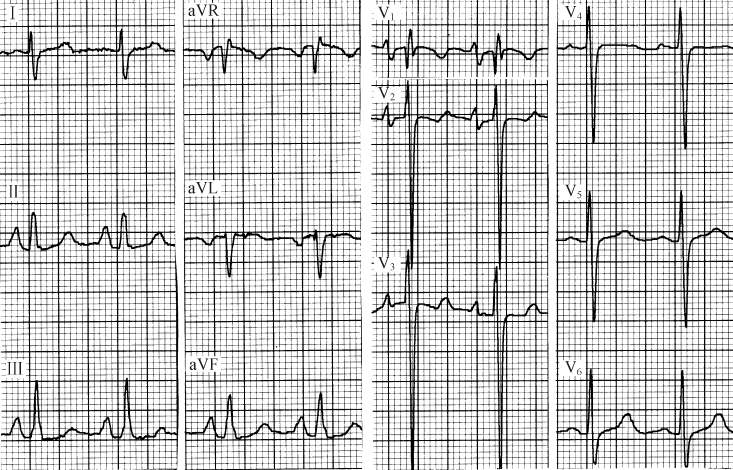
\includegraphics[width=3.36458in,height=2in]{./images/Image00008.jpg}
\end{table}

周围型位置性眩晕、眼震的常见疾病有良性阵发性位置性眩晕(即耳石病)、梅尼埃病、耳硬化症、内耳开窗术后、浆液性迷路炎、内听动脉供血不足、药物性内耳损害等。中枢性位置性眩晕、眼震的常见疾病可见于小脑蚓部肿瘤、第四脑室肿瘤或囊肿、椎-基底动脉供血不足、桥小脑角肿瘤、颅脑外伤等。

\subparagraph{直流电试验}

应用直流电检查前庭神经,电流不仅刺激前庭末梢器,也能直接作用于前庭神经节及前庭神经。方法为将直流电负极置于测试耳的耳屏处或乳突处,正极置于前额或手中,电流逐渐缓慢增加,分别观察出现眩晕感、倾倒及眼震的毫安(mA)数,通常于正常人2~4mA即有眩晕感觉,4~6mA出现倾倒反应,6~8mA出现眼震。眼震之快相向负极侧,而倾倒则向负极之对侧。直流电试验主要的临床价值可协助鉴别前庭末梢器和前庭神经本身的病变。例如前庭末梢器病变(梅尼埃病、迷路炎)变温试验可能显示病侧前庭功能减退或功能消失,而直流电试验仍属正常反应。若病变累及前庭神经例如听神经瘤,则变温试验无反应时,直流电试验亦无反应。

\subparagraph{视动性眼震试验(optokinetic test)}

视动性眼震由固视连续移动景物所引起而非前庭刺激所引起。试验原理:当两眼注视眼前连续而迅速通过的一系列物体时,每一物体在后一物体出现于视野中以前,受到两眼的注视与跟随。而当下一物体的影像落于视网膜的周边部时,眼球即反射性反跳,以便使后一物体像落于黄斑上。眼球如此快慢交替地运动,遂形成视动性眼球震颤,这是一种生理现象。此项检查之所以列入神经耳科学,是因为:①视动性眼震亦有快相与慢相的交替运动,与前庭性眼震形式类似;②此项检查对各种自发性眼震鉴别及颅内病变的定位诊断有一定价值。应用视鼓或视伞或带尺诱发眼球震颤。正常人所诱发之视动性眼震之慢相与视鼓旋转之方向一致,眼震之快相与视鼓旋转之方向相反,所诱发出之视动性眼震向左、右侧是对称的。

一般认为视动性眼球震颤的神经通路为:起自视网膜右半侧之神经纤维→右侧膝状体→视放射→视皮质(Brodman18区、角回和缘上回)的视动中枢,再自视动中枢通过视放射后部深处前行,离视放射→大脑脚→上丘→经内侧纵束→脑桥眼球同向运动中枢→眼球运动核。

因此,皮质视动中枢至脑桥同向运动中枢间任何部位之病变累及视动通路,即可消除或减弱向对侧之视动性眼球震颤,亦即出现向病侧之视动性眼震优势偏向。根据笔者研究的资料分析,在大脑半球占位性病变中,出现视动性眼震优势偏向现象多数与后颞、顶枕部(尤其是顶部)有关。如果病变累及脑干内的视动反射纤维,亦常有异常反应,多数为不对称性异常。在眼源性的自发性眼球震颤病例中,视动性眼震反应多数表现为同向性异常(即眼震的快相与视鼓或视伞旋转的方向相同),或无反应。

\subparagraph{眼震电图(ENG)}

检查对于眩晕患者作前庭功能检查,其中自发性眼球震颤与诱发性眼球震颤都是检查中的一项重要体征,除肉眼观察外,应用眼震电图记录,可以使眼球震颤的各种特征(速度、频率、幅度、方向)客观记录下来,以供比较分析研究。通常所见到的节律型、水平性(或垂直性)眼震在眼震电图上表现为一不对称的峰形波,由迅速上升(或下降)的快相与缓慢回复至基线的慢相所组成。

眼震强度可用眼震时程、幅度、频率、慢相速度等表示,其中以时程和慢相速度为可靠。

慢相速度的测量方法如下:①正常眼震电图测量法:见图\ref{fig3-1}。②眼震强度------慢相速度计算法:其中几何作图法(图\ref{fig3-2})系延长慢相斜边成AC,使BC等于纸速1秒(s),若测得AB
= 22mm,定标值10°=
11mm,按速度=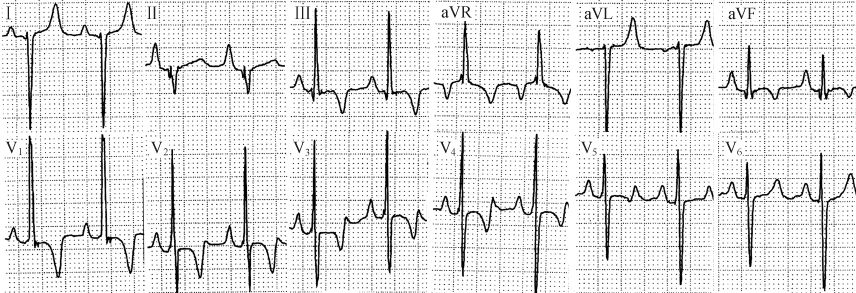
\includegraphics[width=0.30208in,height=0.32292in]{./images/Image00009.jpg}
,得

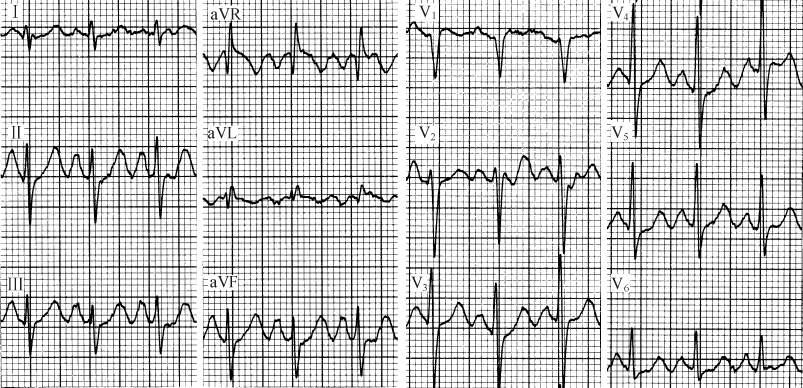
\includegraphics[width=1.95833in,height=0.42708in]{./images/Image00010.jpg}

\begin{figure}[!htbp]
 \centering
 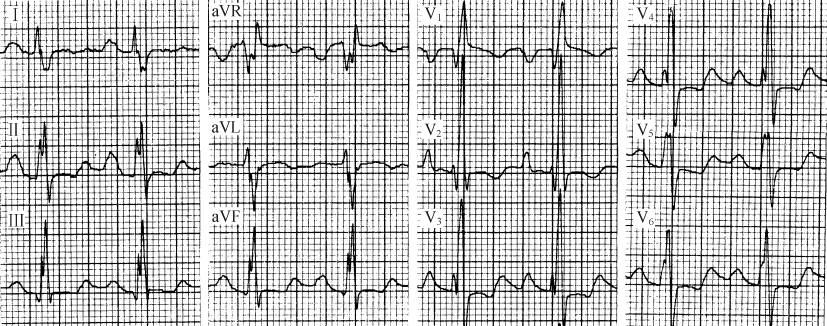
\includegraphics[width=2.75in,height=1.13542in]{./images/Image00011.jpg}
 \captionsetup{justification=centering}
 \caption{正常眼震电图}
 \label{fig3-1}
  \end{figure} 

a.右向眼震;b.左向眼震;c.快相;d.慢相

\begin{figure}[!htbp]
 \centering
 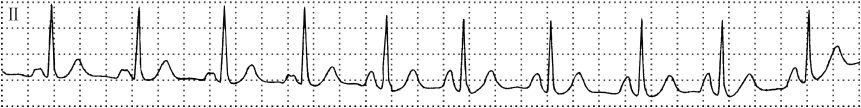
\includegraphics[width=1.96875in,height=1.29167in]{./images/Image00012.jpg}
 \captionsetup{justification=centering}
 \caption{几何作图法}
 \label{fig3-2}
  \end{figure} 

另为极盛期价值法(culmination
valve),于变温试验中,取反应高潮期10秒内之眼震,计算其幅度和频率,以慢相速度表示之。其公式如下:

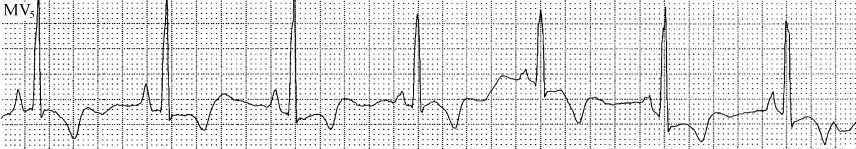
\includegraphics[width=2.16667in,height=0.53125in]{./images/Image00013.jpg}

例如:10秒内眼震总幅为150mm,总次数为20次,定标值10°= 11mm,则

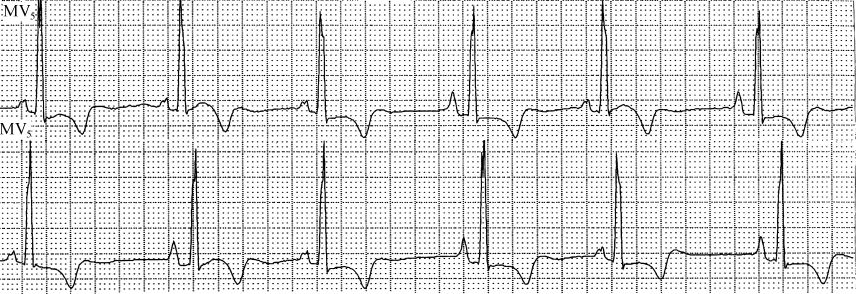
\includegraphics[width=2.57292in,height=0.40625in]{./images/Image00014.jpg}

利用眼震电图可以记录各种自发性眼震,并通过各种诱发试验记录变温性、位置性、视动性、凝视性眼球震颤。并可作扫视试验(saccade
test)、平稳跟踪试验(pursuit
test),于检查中可进一步观察在睁眼(明亮条件下)、暗室中、闭眼条件下眼震的变化。这些客观资料,均有助于对眩晕、眼震、前庭系统疾病的诊断。

\subsubsection{诊断注意事项}

对于临床医师而言,在对眩晕的病因作诊断与鉴别诊断时可先从以下几方面考虑:

1.前庭系统性眩晕抑或非系统性眩晕
一般而言,凡属前庭系统性眩晕均具有空间定向的感觉异常,具有运动错觉或运动幻觉的特点,或觉外境或觉自身在运动感(旋转、摇晃、向一侧移动);而非系统性眩晕则没有上述的特点,大多数患者对“眩晕”描述为头昏、头胀、头重脚轻、头脑内转动等。

2.前庭周围性眩晕抑或前庭中枢性眩晕
对于前庭系统性眩晕应进一步鉴别是前庭周围性病变还是前庭中枢性病变,两者的鉴别见表\ref{tab3-2}。

\begin{table}[htbp]
\centering
\caption{前庭周围性眩晕与前庭中枢性眩晕的鉴别}
\label{tab3-2}
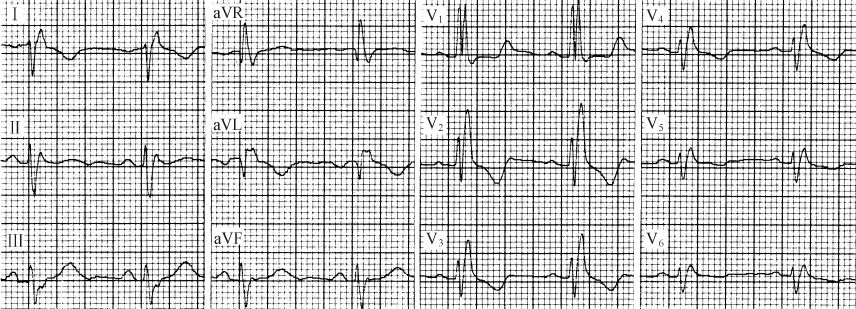
\includegraphics[width=3.3125in,height=2.78125in]{./images/Image00015.jpg}
\end{table}

3.更进一步的诊断需根据各疾病的临床表现的特点及必要的辅助检查。

\subsubsection{常见眩晕症疾患的临床特点}

\hypertarget{text00012.htmlux5cux23CHP1-3-2-6-1}{}
(一) 梅尼埃病(Ménière disease)

梅尼埃病系内耳病变,为中年以上阵发性眩晕的最常见的原因。临床表现为典型的三联症状:发作性眩晕,波动性、渐进性、感音性的听力减退和耳鸣。眩晕发作时常伴有恶心、呕吐、出汗、面色苍白、眼球震颤。眩晕常突然发作,发作前耳鸣增加,听力骤减,耳内有饱胀感。每次眩晕发作历时数小时至数天(多系1~2天)而自行缓解。发作间歇期长短不一,多数为数月一次,亦有一个月数次者。眩晕发作常常随耳聋的进展而减少,至完全耳聋时,迷路前庭功能消失,眩晕发作亦常终止。于眩晕发作间歇期间检查,仅可发现单侧(少数为双侧)感音性耳聋,作电测听检查部分患者重振试验(recruitment
test)呈阳性。前庭功能变温试验于一部分病例中显示功能减退。本病产生的原因可能是支配前庭器的交感神经功能失调引起迷路动脉痉挛,从而使内淋巴产生过多或吸收障碍,导致迷路水肿及内淋巴系压力增高,内淋巴腔扩大及内耳末梢器缺氧、变性等病理变化。

\hypertarget{text00012.htmlux5cux23CHP1-3-2-6-2}{}
(二) 良性发作性位置性眩晕(benign paroxysmal positional
vertigo,BPPV)

本病多见于中年以上患者,多数学者认为是耳石器病变所致,故又称此病为耳石病。患者常诉说当头部处于某一位置时即引起头晕,有些患者诉说半夜翻身时突然发生眩晕,若再回复该头位又即会再发生,因而患者尽可能回避该头位。眩晕严重时伴有恶心、呕吐。常无听力障碍。作头位位置检查,常能在患者所诉说的那个头位引起眩晕,同时可见有短暂的水平兼旋转性眼球震颤,眩晕与眼震一致,持续10~20秒自行缓解。重复该头位可重复出现眩晕与眼震。但于短期内连续数次重复检查,则可逐步适应而不出现眩晕症状与眼震。变温试验提示前庭功能正常。病程常为自限性,数周至几个月后可自愈。近年来一些学者研究认为其基本病理机制系椭圆囊斑上耳石脱落、游离的耳石进入后半规管并在内淋巴内移动,在头位变动时刺激后壶腹嵴,于是乃产生短时间的眩晕。至于耳石器病变的原因主要有:①前庭动脉前支血栓形成;②颅脑外伤致内耳震荡。在作头位位置试验时,重复数次检查后之所以出现适应(疲劳)现象是由于耳石散落在内淋巴腔,一时未能沉积在后壶腹顶部,故不再引起症状,但待耳石沉积在壶腹顶部时可再度诱发位置性眩晕与眼震。

\hypertarget{text00012.htmlux5cux23CHP1-3-2-6-3}{}
(三) 非良性位置性眩晕

颅后窝的占位性病变也可引起位置性眩晕
,这与上述良性位置性眩晕在临床表现上有以下区别:此种眩晕的发生往往在头位改变后立即出现,无潜伏期,诱发之眩晕持续时间较长,往往引起恶心、呕吐,眩晕可在数种头位诱发,而不像BPPV只在较特定的1~2种头位才诱发。常见的疾病是第四脑室、小脑蚓部的肿瘤或第四脑室的囊肿,亦可见于小脑半球、脑桥小脑角的肿瘤。除位置性眩晕外,有时有肢体或躯干的共济失调。

\hypertarget{text00012.htmlux5cux23CHP1-3-2-6-4}{}
(四) 前庭神经元炎(vestibular neuronitis)

起病较急,表现为突起的剧烈的眩晕,伴有恶心、呕吐,但无耳蜗症状。起病时常伴有感染(多为上呼吸道)症状,可能是一种病毒感染。发病时有自发性水平性眼球震颤,躯体平衡失调。变温试验显示病侧前庭功能减退或缺失,有时双侧均有损害。预后良好,一般在数周后眩晕症状逐日减轻,但变温试验示前庭功能呈永久性损害。多数学者认为病变主要为病毒侵犯前庭神经的Scarpa神经节,但也有少数学者认为有时脑干内的前庭纤维也受侵犯。

\hypertarget{text00012.htmlux5cux23CHP1-3-2-6-5}{}
(五) 迷路炎

单纯性中耳炎由于炎症刺激使迷路充血可引起眩晕。眩晕程度较轻,中耳炎好转后眩晕亦即解除。中耳炎并发弥漫性化脓性迷路炎时,眩晕严重,伴恶心、呕吐、眼震及病侧听力严重丧失,病侧前庭功能消失。此外还有耳痛、耳漏、头痛、发热等中耳感染症状与体征。慢性中耳炎侵蚀骨迷路有瘘管形成时,常有反复发作的眩晕。瘘管试验(以希格尔镜利用橡皮球增减外耳道压力,通过瘘管影响迷路,产生前庭反应)呈阳性反应。提示内耳有瘘管存在。

\hypertarget{text00012.htmlux5cux23CHP1-3-2-6-6}{}
(六) 药物性眩晕

在临床药物应用中
,有些药物因使用不当,因毒性作用而致眩晕,如链霉素;有些是难以避免的副作用,如某些镇静药和安眠药;有些是过敏所引起。

\subparagraph{耳毒性抗生素类}

以氨基糖苷类为主,如链霉素(尤其是硫酸链霉素)、新霉素、卡那霉素、庆大霉素、阿米卡星(丁胺卡那霉素)等,其他尚有万古霉素、多黏菌素B。其中有些药物性损害主要影响前庭部分,但大多数前庭与耳蜗均有影响。链霉素是最常见者,引起眩晕症状通常于疗程第4周出现,但亦有仅应用4天即有眩晕症状者。在年老患者或有肾功能不全的患者,更易出现毒性作用。眩晕症状持续,而在患者行走、头部转动或转身时症状更为明显。于静止时、头部不动时,上述症状明显好转,甚至消失。而一旦活动后上述症状又复出现。前庭功能检查,大多数患者均无自发性眼球震颤,闭目难立征阳性,向左右前后摇晃方向不定。变温试验示双侧前庭功能均明显减退或消失。如伴有耳蜗损害,则尚有双侧感音性耳聋。眩晕症状消失较为缓慢,需数月甚或1~2年之久,前庭功能则更难恢复。

\subparagraph{麻醉 、镇静和催眠药}

这类药物引起眩晕的机制主要是对中枢的抑制作用,皮质中枢受抑制时表现为头晕及轻度失平衡,并无明确的运动错觉。于麻醉后,由于皮质中枢的强抑制,有关平衡的各种传入信息,不能在中枢获得综合与分析,因而出现头晕症状,患者诉说昏昏沉沉。这些药物中除麻醉药外还有异丙嗪(非那更)、苯巴比妥(鲁米那)、利眠宁(氯氮{}
)等。

\subparagraph{抗癫痫药}

在抗癫痫药中苯妥英钠与扑米酮是引起眩晕的最常见者,尤其是苯妥英钠,因应用广,应用时间又长,如不注意服用剂量及检测药物血药浓度,则甚易引起中毒性损害。主要损害于前庭末梢器,可累及小脑,均可导致眩晕,平衡失调,眼球震颤,共济失调,因此对于这些患者应定期随访,必要时检测药物血药浓度,调整药物剂量。扑米酮能用于抗痫治疗,虽较少用,但初服此药时,其剂量应减少至甚小量(成人常规用量之1/3~1/4),然后缓慢增加,才可避免眩晕。

\subparagraph{其他药物}

如水杨酸类(水杨酸钠)、噻嗪类利尿剂(氢氯噻嗪)、降压药(利血平、降压灵)及某些磺胺类药均可致眩晕,在临床应用时应予注意。

\hypertarget{text00012.htmlux5cux23CHP1-3-2-6-7}{}
(七) 血管性眩晕(椎-基底动脉血循环障碍)

\subparagraph{迷路卒中}

由于动脉粥样硬化或伴有血液黏稠度增加,血压的偏低,导致内听动脉血栓形成,常产生急骤的、严重的眩晕,伴恶心、呕吐,若耳蜗分支同时受损,则伴有耳聋及耳鸣。患者年龄较大,起病甚快,有身体其他部位动脉硬化的征象,既往(青、中年时)无类似的眩晕发作史等特点,均有助于与其他急性眩晕相鉴别。但有的患者表现短暂性的眩晕发作,伴有或不伴有耳蜗症状,持续数分钟至数小时即缓解,对于这些中、老年患者,若除外耳源性眩晕的其他疾病,可诊断为迷路动脉短暂性缺血发作(TIA)。

\subparagraph{小脑后下动脉血栓形成}

亦称延髓外侧综合征(Wallenberg
syndrome)。其典型的症状与体征包括突起眩晕,伴恶心、呕吐,眼球震颤;病侧肢体共济失调及颈交感神经麻痹综合征;吞咽困难及同侧软腭麻痹、声带麻痹;病侧面部及对侧躯体、肢体的痛温觉减退或消失。

\subparagraph{椎-基底动脉供血不足(vertebrobasilar insufficiency,VBI)}

多数表现为椎-基底动脉的TIA,临床常见。有关本病的概念至今还不十分清楚。引起VBI的病例基础是:①椎动脉的解剖特点:起始于两侧锁骨下动脉之椎动脉,需穿过第6~1颈椎横突孔后再经枕大孔入路,然后合并为基底动脉,椎动脉在行程中需经过一条活动度较大的骨性隧道。②椎动脉易发生动脉粥样硬化,随着年龄增大其动脉管径逐渐变窄,血流量亦渐变少。③中年以后颈椎常发生退行性变及骨赘形成。因此椎动脉的血流易受到各种因素的影响,例如颈部的转动,血压的较快的降低,血管的痉挛,血黏度的增高。因此VBI的发病通常认为主要是动力学改变所致,但也有部分患者VBI是由于循环系统内的微栓子所造成。由于迷路、前庭神经核、小脑的血液供应均来源于椎-基底动脉血流循环,因此VBI的主要临床表现是眩晕,常突然发生,颈部过度伸屈或旋转有时可诱发,眩晕发作持续通常短暂,常常数分钟即缓解,但可在短时期内反复发生多次,眩晕发作时可伴有恶心、呕吐、站立不稳,亦可伴有椎-基底动脉的其他供应区缺血的临床征象,例如视幻觉、偏盲、猝倒发作、复视、面麻木、进食吞咽困难,肢体肌力减退或感觉障碍,共济失调。上述这些临床表现通常都是呈发作性、短暂性,症状持续数分钟至数小时,不超过24小时,这一类型的VBI可称之为VBTIA(椎-基底动脉短暂性缺血性发作),但临床上也有一部分患者表现为在一段时期内(数天至数周)经常性的头晕,行走不稳,在除外了其他引起眩晕的疾病后亦应考虑为VBI,推究其发病机制是后循环的动力学障碍所致,应予重视。

对于VBI的诊断应根据具体情况选择作下列检查:①颈椎X线片,包括正、侧及斜位片,以发现有无颈椎病及其严重程度及了解有无骨刺可能累及椎动脉。②颈椎CT或颈椎MRI或螺旋CT,以进一步了解颈椎骨骼及脊髓和有关椎动脉受压、变窄情况。③头颅MRA,以了解颅内血管情况,尤其是了解椎-基底动脉及颅内脑底动脉环情况。④TCD检查。⑤BAEP检查。⑥SPECT检查。上述三项检查在VBI的病例中均有相当的阳性率,可作为诊断的参考依据。⑦前庭功能检查主要是作变温试验,对于了解前庭功能有肯定的价值。⑧眼震电图检查:可作扫视试验、凝视试验、跟踪试验、视动试验。有一定的临床价值。

关于椎-基底动脉短暂性缺血性发作的诊断依据:①中老年患者(发病在50岁以上)。②发作性眩晕,每次持续时间短暂,通常为数分钟至数十分钟。③眩晕发作时可伴有一种或数种脑干、小脑、枕叶的缺血症状及体征。④临床症状除轻度眩晕,行走不稳外均在24小时内减轻以至消失。⑤实验室检查(上已述及)有两项以上的阳性发现。⑥排除引起眩晕的其他病因。

\subparagraph{颈椎病变}

颈椎退行性病变导致椎间隙狭窄,及由于钩椎关节骨赘增生刺激或压迫椎动脉,使椎动脉痉挛、阻塞,当转颈时一侧之椎动脉更易受压。若椎动脉本身已有粥样硬化,一侧椎动脉受压后,对侧椎动脉无法代偿则出现症状。临床常见之症状为发作性眩晕,其发病与头颈转动有密切关系。此外,这些患者尚可伴有枕部头痛、猝倒、视觉症状(闪光、视野缺失)及上肢麻痛。颈椎X线片、颈CT扫描可显示颈椎形态学病变改变。

\hypertarget{text00012.htmlux5cux23CHP1-3-2-6-8}{}
(八) 颅内肿瘤

由于颅内肿瘤所产生的眩晕有两种机制
:一是由于肿瘤直接压迫、浸润前庭神经或其中枢连接;另一是由于颅内压增高,尤其是由于肿瘤阻塞脑脊液循环而产生脑积水,引起第四脑室底部前庭核的充血和水肿。

\subparagraph{桥小脑角肿瘤}

特别是听神经瘤,有轻度眩晕和耳鸣、耳聋,这是听神经瘤的早期症状。病变进一步发展可出现邻近脑神经受损的体征,如病侧角膜反射减退、面部麻木及感觉减退,展神经麻痹、周围性面瘫、眼球震颤,同侧肢体共济失调。在听神经瘤的早期通常并没有自发性眼球震颤,当肿瘤增大压迫脑干或小脑时才会出现,但一经出现则持续存在。听神经瘤至病程后期还可出现颅内压增高症状,头痛、视神经乳头水肿。对于听神经瘤的早期诊断可根据单侧性听力渐进性减退、听力检查为感音性耳聋;同侧前庭功能早期即消失,邻近脑神经(三叉、展、面神经)中有一根受累即应考虑为听神经瘤。若脑脊液中蛋白质含量增加,X线片上示病侧内听道扩大诊断即可肯定。近年来由于应用头颅CT及MRI检查,更易得到早期确诊。

\subparagraph{脑干}

(延髓脑桥)肿瘤
因病变累及前庭神经核,常有眩晕及持久的眼震,可有一侧或双侧听力减退,水平性眼震的方向通常为双向性,向左侧注视时快相向左,向右侧注视则快相向右,也可能兼有旋转性眼震。当眼震明显时,眩晕症状不一定很重。还可以有其他脑神经障碍(主要为第Ⅴ、Ⅵ、Ⅶ、Ⅹ、Ⅺ)及对侧肢体瘫痪。

\subparagraph{小脑半球肿瘤}

常有眩晕,早期即出现明显的振幅粗大的眼球震颤,及病侧肢体共济失调,水平性眼震的方向通常是两侧性的,但主要是向病变一侧。前庭功能变温试验示病侧肢体偏斜反应不明显。

\subparagraph{小脑蚓部肿瘤及第四脑室肿瘤}

(或囊肿)
眩晕为常见症状,眩晕的发生或加重常与头位位置有关。作头部位置试验,可见有中枢型位置性眼球震颤,并有早期颅内压增高及固定头位等临床表现。

\subparagraph{天幕上肿瘤}

通常并不出现眩晕,如有则可能与颅内压力增高有关,但颞叶肿瘤有时可出现以眩晕为主要表现的癫痫样发作。脑电图上可以有痫样发放。

\hypertarget{text00012.htmlux5cux23CHP1-3-2-6-9}{}
(九) 外伤性眩晕

颅脑外伤时可因内耳迷路
、第Ⅷ脑神经、中枢前庭核及其中枢连接受损而产生眩晕。这些结构可单独或合并受损。迷路内外伤性出血的患者有周围型的前庭紊乱症状,常有颞骨骨折及听力同时受损的征象。亦有内耳并无出血而为迷路震荡者,则眩晕症状持续时间短、恢复较快,听力障碍程度亦较轻。部分患者可由于耳石器损伤而出现短期的位置性眩晕。颞骨横行骨折,骨折线横断岩锥,可产生听神经直接受损,出现明显的眩晕、自发性眼震、听力丧失,于4~6周内前庭症状逐渐消失,但听力常难以恢复。

严重的颅脑损伤患者,在第四脑室及导水管周围可见有点状的少量出血,损伤涉及前庭核及其中枢连接。脑干损伤后产生眩晕的同时常伴有脑干损伤的其他体征,如复视、面瘫、瞳孔不等大、肢体运动或感觉障碍等。眩晕症状持续较久,可达数月以上。颈部鞭索样损伤后亦常有眩晕症状,在头部运动时,尤其是向着颈部鞭索样受损的方向运动时,眩晕症状更易出现。每次眩晕发作数秒至数分钟。头位位置试验可有位置性眼震,常发生于头部转向鞭索样损伤侧,可能是由于内耳耳石器受损所致。

\hypertarget{text00012.htmlux5cux23CHP1-3-2-6-10}{}
(十) 精神性眩晕

精神性眩晕在本质上是神经症的一种表现。大多感觉头昏脑胀,非真性眩晕,无运动错觉,患者诉“眩晕”、“头晕”时无自发性眼震或自发性倾倒,往往常有神经症其他表现如失眠、焦虑、紧张、记忆力减退、注意力难集中等。无前庭系或非前庭系器官性疾病。起病诱因系以情绪、精神因素为主。

\subsection{处理原则}

\subsubsection{一般处理}

对于急性眩晕发作的患者,需卧床休息,饮食以流质为宜。伴有明显恶心、呕吐者,应酌情给予静脉补液,以维持营养,并需注意水、电解质的平衡。对于焦虑紧张的患者,应给予适当的病情解释与安慰,以解除顾虑。眩晕发作缓解后,应鼓励患者早日逐渐参加日常活动,适应日常生活。

\subsubsection{病因治疗}

因中耳炎并发症引起的急性化脓性迷路炎,应由耳科作必要的手术及抗感染治疗。由颅内占位性病变如小脑肿瘤、听神经瘤引起者,需作手术摘除肿瘤。由于梅尼埃病产生的眩晕,主张调节自主神经功能,平时以低盐饮食为宜。对于由药物中毒性损害引起的眩晕患者,应及时停药,并给予维生素B族药物。因颈椎骨质增生、椎间盘膨隆或突出而致的眩晕,可先作颈椎牵引或作颈托固定。必要时再考虑手术治疗。因心律失常或血压过高、偏低者,则需给予相应的内科治疗。因贫血引起的眩晕应纠正贫血。凡此种种的有关病因的处理均属重要,不可忽视。

\subsubsection{对症处理}

在病因治疗的同时,对于眩晕症状需给予药物治疗,以减轻眩晕症状及减少伴发的恶心、呕吐、焦虑、紧张等症状。

\subparagraph{急性发作期的药物治疗}

可考虑选用的药物有:氢溴酸东莨菪碱0.3mg,肌肉注射;茶苯海明(晕海宁,dramamine)50mg,肌肉注射;硫酸阿托品0.5~1mg,肌肉注射;山莨菪碱(654-2)5~10mg,肌肉注射;盐酸异丙嗪(非那更)25~50mg,肌肉注射。以上药物可选择应用,并可根据病情每隔4~6小时重复给药2~3次。

\subparagraph{眩晕发作后尚有轻度症状或慢性眩晕的治疗}

在急性眩晕发作后,虽已无明显的旋转幻觉,但仍有平衡失调、站立不稳的感觉,或在头部、身体转动时有这些症状,或眩晕程度虽轻但经常存在者,可选用各种镇静剂、安定剂,例如苯巴比妥0.015~0.03g,或地西泮(安定)2.5~5mg,或氯丙嗪25mg等,均为每天2~3次,口服。

\subparagraph{几种治疗眩晕症的常用药物}

\hypertarget{text00012.htmlux5cux23CHP1-3-3-3-3-1}{}
(1) 镇静剂与安定剂:

例如苯巴比妥、溴剂、地西泮等。它们的药理作用对于前庭反应有抑制作用,对于一般感觉亦起抑制作用,因此可以减轻眩晕症状,消除紧张、烦躁不安、焦虑等症状。苯巴比妥虽可以减轻眩晕,但也常有全身抑制的作用,如疲倦、乏力。地西泮能减轻眩晕症状,减少紧张、焦虑,并有止吐作用,但可加强其他中枢抑制剂的作用。大剂量的安定类药物可以引起锥体外系的副作用。

\hypertarget{text00012.htmlux5cux23CHP1-3-3-3-3-2}{}
(2) 抗组胺药物:

例如苯海拉明、盐酸异丙嗪、氯苯那敏、盐酸氯苯苄嗪(敏克静)、茶苯海明等,这些药物用于治疗眩晕,其治疗效应可能是由于它们药理上的镇静作用而不是抗组胺作用。它们应用于眩晕发作期尚有止吐作用。

\hypertarget{text00012.htmlux5cux23CHP1-3-3-3-3-3}{}
(3) 止吐剂:

常用者为盐酸氯苯苄嗪及异丙嗪,均有明显止吐作用,适用于运动病及眩晕时伴有明显的自主神经反应(恶心、呕吐)的病例。这些药物亦有镇静作用及抗组胺作用。

\hypertarget{text00012.htmlux5cux23CHP1-3-3-3-3-4}{}
(4) 抗胆碱药物:

常用药物系东莨菪碱与阿托品,对于梅尼埃病的治疗效果较好。这类药物尚有止吐及解除血管痉挛的作用。东莨菪碱还有镇静作用,可优选使用。

\hypertarget{text00012.htmlux5cux23CHP1-3-3-3-3-5}{}
(5) 血管舒张药物:

例如烟酸、妥拉唑啉、山莨菪碱、地巴唑,这些药物并不是前庭抑制药物,其药理作用为解除血管痉挛。可应用于因血管痉挛、缺血性病变所引起的眩晕,如梅尼埃病的发作期及椎-基底动脉供血不足的病例。此外倍他司汀(betahistine,抗眩啶)亦有扩张血管的作用,常用量为4mg,每日3次;甲磺酸倍他司汀(敏斯朗)亦有类似的作用,6mg,每日3次口服。

\hypertarget{text00012.htmlux5cux23CHP1-3-3-3-3-6}{}
(6) 钙拮抗剂:

目前常用者有尼莫地平20mg,每天3次;桂利嗪(脑益嗪)25mg;每天3次,氟桂利嗪(flunarizine,商品名西比灵)5mg,每天1~2次,均为口服。

\hypertarget{text00012.htmlux5cux23CHP1-3-3-3-3-7}{}
(7) 增强动脉血氧分压和血氧饱和度药物:

阿米三嗪萝巴新{[}都可喜(Duxil){]}内含阿米三嗪和萝巴新,本药可增迷路和脑组织的血氧供应,对于因缺血缺氧而产生的眩晕疾患有较好的疗效,常用量为30mg,每天2次,口服。


\hypertarget{text00013.htmlux5cux23CHP1-3-4}{}
参 考 文 献

1. 史玉泉.实用神经病学.第3版.上海:上海科学技术出版社,2004

2. Norre ME. Clinical value of caloric test. Clin
Otolaryngol,1988,13:247

\protect\hypertarget{text00014.html}{}{}

\chapter{晕 厥}

晕厥(syncope)又称昏厥,是由于短暂的全脑组织灌注降低而导致的一过性意识丧失(transient
loss of
consciousness,TLOC),以快速发作、持续时间短和自限性为特点。可因血管迷走反射、直立性低血压、心输出量减少引起全脑低灌注,或由于脑干椎-基底动脉缺血引起脑干选择性低灌注所致。晕厥发作起病突然,持续时间短,典型可分为三期,其基本临床特点为:①发作前期:患者常感头部及全身不适、头晕、视力模糊、耳鸣、面色苍白、出汗,预示即将发生晕厥;此时患者如取头低位躺卧姿势常可防止发作。②发作期:轻者眩晕、恶心、躯体发软,眼前发黑,重者常突然意识丧失,全身肌紧张度消失,跌倒地上。意识丧失超过15~20秒可发生阵挛动作,有时有呼吸暂停,心率减慢,甚至心脏暂停搏动,瞳孔散大,流涎,尿失禁等;其特点是发作时间短暂,一般持续1~2分钟左右。脑电图检查可见持续3~10秒的广泛性、对称性2~3Hz的慢波。③发作后期(恢复期):患者平卧后意识迅速恢复(数秒至数分钟),可遗留紧张、头晕、头痛、恶心、苍白、出汗、无力和便意感等,甚至呕吐及括约肌失禁。休息数分或数十分钟缓解,不留后遗症,偶有极短暂的(<
30秒)发作后模糊状态伴定向力障碍和易激惹。

可见晕厥的特征是:发作突然,意识丧失时间短,不能维持正常姿势或倒地,在短时间内迅速恢复,罕有后遗症。

当前急诊对晕厥的评估已经从诊断晕厥的病因转变为进行危险分层,其目的是:①识别有威胁生命的疾病并收入院;②识别低危患者,可以让他们离院,并且以后到专科就诊;③识别不需要进一步诊断和治疗的患者;④对初步评估不能得出结论的患者进行进一步检查。

\subsection{病因与发病机制}

引起晕厥的病因很多(表\ref{tab4-1}),但任何原因均是通过影响脑血流,引起脑血供障碍所致。人脑重量占体重的2\%,而脑耗氧量却占全身耗氧量的20\%。脑组织几乎无氧和葡萄糖储备,全靠血循环提供外源性补给才能维持其正常的生理功能。健康成人的脑血流量为每100g脑组织45~50ml/分钟,而维持人的意识水平所需最低限度的脑血流量(即临界值)为每100g脑组织30ml/分钟,当脑血流量骤减至此临界值则可发生晕厥。

\subparagraph{反射性晕厥(神经介导的晕厥)}

此类晕厥主要由于在正常状态下控制循环系统的心血管反射对刺激因素出现间歇性的不恰当反应,引起血管扩张和(或)心动过缓,导致动脉血压降低及全脑灌注减少。依据诱发因素不同又可分为以下几类:

\begin{table}[htbp]
\centering
\caption{晕厥的病因分类}
\label{tab4-1}
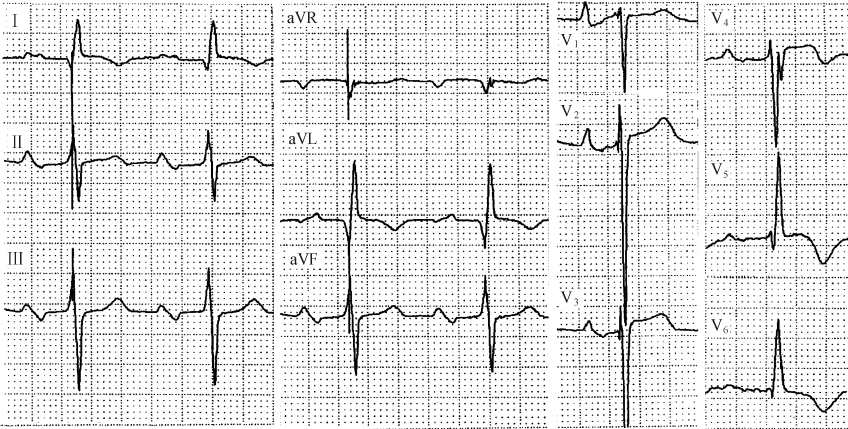
\includegraphics[width=3.30208in,height=7.11458in]{./images/Image00017.jpg}
\end{table}

\hypertarget{text00014.htmlux5cux23CHP1-4-1-1-1}{}
(1) 血管迷走性晕厥:

是最常见的晕厥类型,由情绪或直立位诱发,常伴自主神经激活的前驱症状(大汗、苍白或恶心)。

\hypertarget{text00014.htmlux5cux23CHP1-4-1-1-2}{}
(2) 情境性晕厥:

与一些特殊情境相关,如运动后晕厥等。

\hypertarget{text00014.htmlux5cux23CHP1-4-1-1-3}{}
(3) 颈动脉窦晕厥:

常由非机械性刺激因素诱发,可通过颈动脉窦按摩来确诊。

\hypertarget{text00014.htmlux5cux23CHP1-4-1-1-4}{}
(4) 不典型晕厥:

多数没有明确的诱发因素,诊断主要基于排除其他晕厥的病因(无器质性心脏病)。

\subparagraph{直立性低血压和直立性不耐受综合征}

此类晕厥主要包括以下4种类型:

\hypertarget{text00014.htmlux5cux23CHP1-4-1-2-1}{}
(1) 典型的直立性低血压(OH):

站立3分钟内,收缩压下降≥20mmHg和(或)舒张压下降≥10mmHg,见于单纯性自主神经功能衰竭(ANF)、低血容量或其他形式的ANF。

\hypertarget{text00014.htmlux5cux23CHP1-4-1-2-2}{}
(2) 初始性直立性低血压:

站立即刻血压下降>
40mmHg,然后自发、快速地恢复正常,低血压及其症状持续时间较短(<
30秒)。

\hypertarget{text00014.htmlux5cux23CHP1-4-1-2-3}{}
(3) 延迟(进展性)OH:

其在老年人中并不少见,主要与年龄相关的代偿反射受损有关,以直立状态下收缩压进行性缓慢下降为特点,但不伴心动过缓。

\hypertarget{text00014.htmlux5cux23CHP1-4-1-2-4}{}
(4) 体位性直立性心动过速综合征:

部分患者(主要为年轻女性),表现为严重的直立性不能耐受,但没有晕厥,伴随心率明显加快(增加>
30次/分或达到120次/分以上)和血压不稳定,病理生理机制尚不明确。

\subparagraph{心源性晕厥}

\hypertarget{text00014.htmlux5cux23CHP1-4-1-3-1}{}
(1) 心律失常性晕厥:

是心源性晕厥的最常见病因。心律失常诱发血流动力学不稳定,导致心输出量及脑血流量严重减少。心律失常类型包括:病窦综合征(窦房结功能受损,产生窦性停搏及窦房阻滞,以及慢-快综合征)和严重的获得性房室传导阻滞(莫氏Ⅱ型、高度及完全性房室传导阻滞),也可见于药物引起的缓慢性或快速性心律失常,如延长QT间期药物引起的尖端扭转性室速。

\hypertarget{text00014.htmlux5cux23CHP1-4-1-3-2}{}
(2) 器质性心脏病:

主要见于左室流出道梗阻性疾病。

\subsection{流行病学}

晕厥在普通人群中常见,首发年龄多为10~30岁,其中女性约47\%、男性约31\%在15岁左右发生晕厥。迷走性晕厥是导致晕厥的最主要原因,心源性晕厥是导致晕厥的第二位原因。医院中的老年患者心源性晕厥发病率较高。在小于40岁的患者中,OH所导致的晕厥较为少见。个别患者的病情较为复杂,在医疗转诊、救治的过程中,一些非晕厥的意识丧失患者常被误诊为晕厥。需注意的是,反射性晕厥是年轻人群中最为常见的导致TLOC的原因;而老年患者通常病情较为复杂,且相关病史也不及年轻人群可靠。

\subsection{诊断思路}

晕厥的诊断目的包括:①找出确切的原因以便进行有效的、针对病理机制的治疗;②识别患者的风险,这种风险常取决于潜在的疾病,而不是晕厥本身的机制。

\subsubsection{初步评估}

详细的病史询问在多数情况下有助于鉴别晕厥与非晕厥,但有时非常困难,应包含以下问题:

(1) 是否为完全性意识丧失(LOC)?

(2) LOC是否为一过性,伴快速起病及短暂持续?

(3) 患者晕厥是否为自发性、完全恢复且不留后遗症?

(4) 患者是否丧失肌张力?

若上述问题的答案均为肯定的,则晕厥可能性极大。若≥1个问题的答案为否定,则应首先排除其他类型的LOC。

对出现TLOC的患者进行初步评估,除了过去提出的详细询问病史、体格检查(包括测量不同体位血压)以及心电图检查外。提出在此基础上,可以适当增加其他的检查以保证诊断准确:①40岁以上患者建议首先进行颈动脉窦按摩。②对于有心脏病病史或怀疑此次晕厥与器质性心脏病或其他心血管疾病有关的患者,建议进行超声心动图检查。③对于怀疑因心律失常而导致晕厥的患者,应给予实时心电监测。④若晕厥与体位变化有关或怀疑反射性晕厥时,则应进行相关检查。如卧立位试验和(或)直立倾斜试验等。⑤仅在怀疑非晕厥原因造成的TLOC的情况下,进行神经科检查或血液检查。

当初步评估后尚无法明确晕厥原因时,要求立即对患者的主要心血管事件及心源性猝死(SCD)的风险进行评估。具体流程如图\ref{fig4-1}所示。

根据最新的SCD防治指南对晕厥进行了危险分层,见表\ref{tab4-2}。

经过初步评估有些晕厥即可明确诊断,其诊断的建议及级别、证据水平见表\ref{tab4-3}。

\begin{table}[htbp]
\centering
\caption{晕厥的危险分层}
\label{tab4-2}
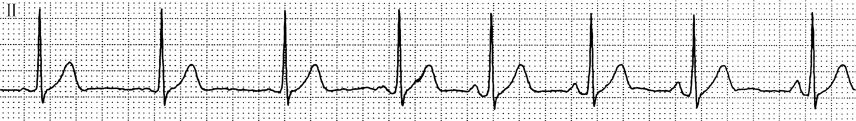
\includegraphics[width=3.28125in,height=4.04167in]{./images/Image00018.jpg}
\end{table}

注:LVEF:左室射血分数,SCD =心源性猝死,VT =室性心动过速,LBBB
=左束支传导阻滞,RBBB =右束支传导阻滞,ARVC
=致心律失常性右室心肌病,心衰=心力衰竭,心梗=心肌梗死

\begin{figure}[!htbp]
 \centering
 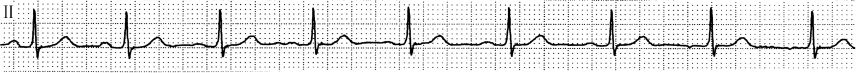
\includegraphics[width=3.84375in,height=3.08333in]{./images/Image00019.jpg}
 \captionsetup{justification=centering}
 \caption{疑似TLOC患者的诊断流程图}
 \label{fig4-1}
  \end{figure} 

\begin{table}[htbp]
\centering
\caption{通过初步评估获得诊断的建议\textsuperscript{*}}
\label{tab4-3}
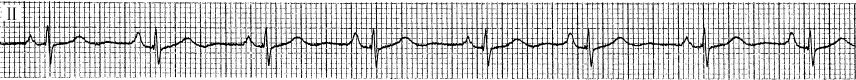
\includegraphics[width=6.66667in,height=2.69792in]{./images/Image00020.jpg}
\end{table}

*本文的建议均源自2009年ESC晕厥诊断和治疗指南。

建议的级别如下:

Ⅰ级:证据和(或)一致同意给予的诊断操作/处理有益,有用和有效。

Ⅱ级:抵触的证据和(或)关于处理的有用/有效存在分歧的观点。

Ⅱa级:证据/观点偏重于有用/有效。

Ⅱb级:证据/观点偏重于无用/无效。

Ⅲ级:证据或一致同意处理无用/无效,且在某些情况下可能有害。

证据水平如下:

A类证据:数据来自多中心随机临床试验或荟萃分析。

B类证据:数据来自单中心随机临床试验或大的非随机研究。

C类证据:专家的一致观点和(或)小的研究,回顾性研究,注册中心资料。

\subsubsection{诊断试验}

初步评估后,倾向性诊断需要进一步检查证实,包括心脏评估检查如超声心动图,心脏负荷试验,心电监测包括Holter,必要时埋藏植入式心电事件记录仪(ILR)和电生理检查;神经介导方面的检查包括倾斜试验和颈动脉窦按摩。

\subparagraph{颈动脉窦按摩}

压迫颈动脉分叉处能够产生反射性心率减慢和血压下降。某些晕厥患者,特别是>
40岁的患者,可以见到对颈动脉窦按摩的异常反应。室性停搏持续≥3秒,收缩压下降≥50mmHg为异常反应,称为颈动脉窦过敏。颈动脉窦按摩是揭示颈动脉窦过敏综合征晕厥的一种检查方法。2009年ESC晕厥诊断和治疗指南颈动脉窦按摩的适应证和诊断标准见表\ref{tab4-4}。

\begin{table}[htbp]
\centering
\caption{颈动脉窦按摩的适应证和诊断标准}
\label{tab4-4}
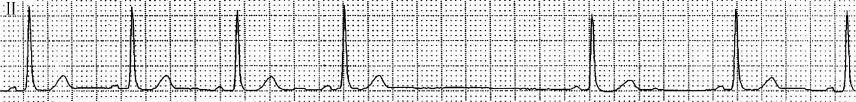
\includegraphics[width=3.34375in,height=1.98958in]{./images/Image00021.jpg}
\end{table}

\subparagraph{倾斜试验}

倾斜试验有助于诊断神经介导性晕厥,但是,其敏感性、特异性、诊断标准和重复性存在很大问题,敏感性和特异性与检查方法有密切关系。敏感性26\%~80\%,特异性约90\%。2009年ESC晕厥诊断和治疗指南倾斜试验的适应证和诊断标准见表\ref{tab4-5}。

\subparagraph{心电图}

(ECG)监测
ECG监测是诊断间歇性缓慢和快速心律失常的方法,但是ECG监测技术目前仍有严重的局限性。晕厥患者ECG监测的作用不是孤立的。医生可以根据病史、体格检查和其他客观检查如倾斜试验决定治疗方案。有些情况下,临床上强烈提示为反射性晕厥时,无需动态心电图(Holter)监测。如果症状发作不频繁Holter监测对诊断意义也不大,这种情况下应考虑植入式循环记录仪。将来的技术可能会记录ECG以外的多项指标,将把重点放在与自发性晕厥相关的心律方面,而不是被触发的晕厥。了解自发性晕厥发作过程是评估晕厥的最好标准。因此,植入式监测仪对晕厥越来越重要。记录到晕厥时有缓慢心律失常即可考虑诊断,但是,有时需要进一步检查明确是心脏本身原因所致还是神经反射机制造成,而反射性心动过缓可能是阵发性心动过缓最常见的原因。

由于晕厥发作时ILR记录到的心律失常的变异和干扰很大,2009年ESC晕厥诊断和治疗指南采用国际不明原因晕厥研究调查组织(ISSUE)的方法,将心电图记录进行了分类,根据主要心律失常和可能的晕厥机制将心电图划分为4型。

1型:心脏停搏,RR间期≥3秒。1型又分为A、B、C
3个亚型。1A型:窦性停搏,表现为进行性窦性心动过缓或初为窦性心动过速逐渐进展为窦性心动过缓直至发生窦性停搏,其可能的机制为反射性。1B型:窦性心动过缓合并房室传导阻滞,表现为进行性窦性心动过缓随后出现房室传导阻滞(和心室停搏)的同时伴有窦率下降;或突发房室传导阻滞(和心室停搏)伴窦率下降,其可能机制为反射性。1C型:房室传导阻滞,突发房室传导阻滞(和心室停搏)伴窦律逐渐增加,其可能机制为自身病变。

2型:心动过缓,心率下降> 30\%或心率<
40次/分持续超过10秒,其可能机制为反射性。

3型:无或很小的心率变异性,心率变异度< 30\%且心率>
40次/分,其机制不肯定。

4型:心动过速,心率增加> 30\%,心率> 120次/分。此型又分为A、B、C、D
4型。4A型:进行性窦性心动过速,机制不肯定。4B型:心房颤动(简称房颤)。4C型:SVT(不包括窦性)。4D型:VT。

\begin{table}[htbp]
\centering
\caption{倾斜试验的适应证和诊断标准}
\label{tab4-5}
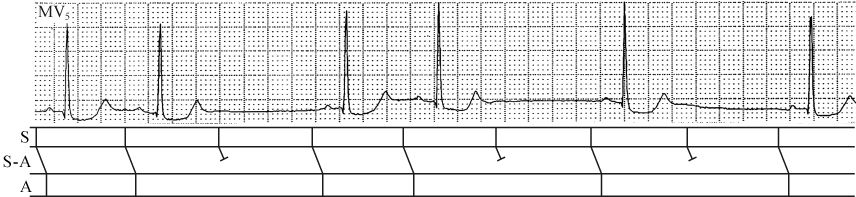
\includegraphics[width=3.21875in,height=6.40625in]{./images/Image00022.jpg}
\end{table}

2009年 ESC晕厥诊断和治疗指南心电图监测的建议见表\ref{tab4-6}。

\subparagraph{电生理检查}

电生理检查通过心内膜和心外膜(冠状窦电极)刺激并记录揭示引起晕厥的原发性心律失常的心电异常改变。然而,仅有少数研究应用Holter和植入式记录仪证实了电生理检查的结果。电生理检查揭示的真实诊断仅仅涵盖了一部分患者。下列诊断标准广泛用于确定窦房结功能障碍:窦房结恢复时间(SNRT)>
1.6秒或2秒或校正的窦房结恢复时间(CSNRT)> 525毫秒。另一项研究认为SNRT
>
3秒诊断窦房结功能障碍性晕厥的可能性更大。2009年ESC晕厥诊断和治疗指南电生理检查的适应证见表\ref{tab4-7}。

\begin{table}[htbp]
\centering
\caption{心电图监测的建议}
\label{tab4-6}
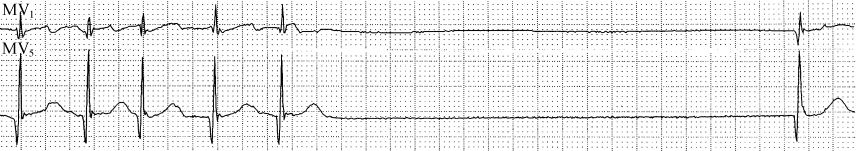
\includegraphics[width=3.25in,height=3.30208in]{./images/Image00023.jpg}
\end{table}

\begin{table}[htbp]
\centering
\caption{电生理检查的适应证}
\label{tab4-7}
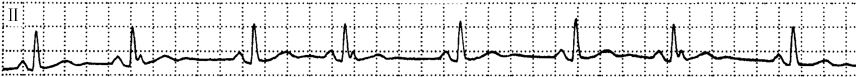
\includegraphics[width=3.25in,height=2.9375in]{./images/Image00024.jpg}
\end{table}

注:ARVC:致心律失常型右室心肌病;HCM:肥厚型心肌病

\subparagraph{超声心动图(UCG)}

当病史、体格检查和心电图检查不能发现晕厥的原因时,超声心动图检查是发现包括瓣膜病在内的器质性心脏病的有效方法。通过该检查还能发现肺动脉高压和右心室扩大等提示肺栓塞的表现。体格检查正常的晕厥或先兆晕厥患者超声心动图检查最常见的发现是二尖瓣脱垂(4.6\%~18.5\%)。其他心脏异常包括瓣膜病(最常见的是主动脉瓣狭窄)、心肌病、节段性室壁运动异常提示的心肌梗死、冠状动脉畸形、浸润性心脏病如淀粉样变性、心脏肿瘤、动脉瘤、左房血栓等。超声心动图检查为判断晕厥的类型、严重程度及危险分层提供重要的信息。如果发现中重度器质性心脏病应考虑心源性晕厥。另一方面,如果超声心动图仪发现轻微心脏结构病变,则心源性晕厥的可能性较小,应进行非心源性晕厥方面的检查。2009年ESC晕厥诊断和治疗指南UCG适应证和诊断标准见表\ref{tab4-8}。

\begin{table}[htbp]
\centering
\caption{UCG适应证和诊断标准}
\label{tab4-8}
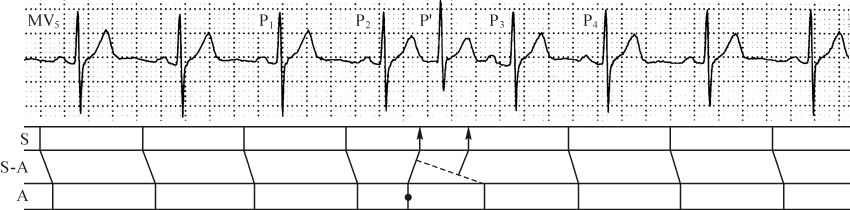
\includegraphics[width=3.20833in,height=1.6875in]{./images/Image00025.jpg}
\end{table}

\subparagraph{运动试验}

运动中或运动后即刻发生晕厥的患者应进行运动试验。进行运动试验应该是症状限制性的,即由于运动中和运动后即刻易发生晕厥,运动中和恢复阶段均应监测心电和血压,应做好防范。运动中发生晕厥可能是心脏原因造成的,有些病例报告运动中也可能发生过度反射性血管扩张引起晕厥,反射性晕厥的元凶是低血压而无心动过缓。相反,运动后晕厥几乎都是自主神经功能异常或神经介导机制参与的,其特点是与心动过缓或心脏停搏有关的低血压;一般发生于无心脏病的患者。运动试验用于诊断神经反射性晕厥,其特点是劳力后晕厥。血管迷走神经性晕厥的患者,运动中内脏容量性血管和前臂阻力血管反射性收缩功能障碍。运动试验对一般晕厥患者意义不大,仅有1\%发现异常。尽管如此,对运动性晕厥具有重要诊断价值。2009年ESC晕厥诊断和治疗指南运动试验的适应证和诊断标准见表\ref{tab4-9}。

\begin{table}[htbp]
\centering
\caption{运动试验的适应证和诊断标准}
\label{tab4-9}
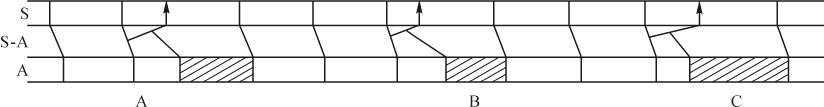
\includegraphics[width=3.25in,height=1.76042in]{./images/Image00026.jpg}
\end{table}

\subparagraph{心导管检查}

心导管检查包括评估心腔形态的心室造影、了解冠脉解剖的冠状动脉造影和了解血流、血管内压力和心腔内压力的血流动力学检查。由于是有创检查,一般不作为筛查心源性晕厥的检查。这些检查能够揭示冠状动脉狭窄引起缺血性晕厥:室壁运动异常和心肌收缩力减弱;缺血引起的心律失常、心脏停搏或完全性房室阻滞和缺血诱发的血管迷走神经性反应。也可以揭示冠状动脉痉挛引起的晕厥,这种患者冠状动脉造影中应做麦角新碱试验。

\subparagraph{神经系统检查}

神经系统疾病引起的晕厥有三种情况。①自主神经功能障碍:晕厥可以是自主神经系统疾病和功能不全的结果;②有些脑血管疾病也可以引起晕厥(大多是“窃血”综合征);③有些疾病应列为鉴别诊断的内容,因为这些疾病可以引起短暂意识丧失(但不是晕厥,如癫痫)或其发作类似于意识丧失。2009年ESC晕厥诊断和治疗指南神经系统检查适应证见表\ref{tab4-10}。

\begin{table}[htbp]
\centering
\caption{神经系统检查适应证}
\label{tab4-10}
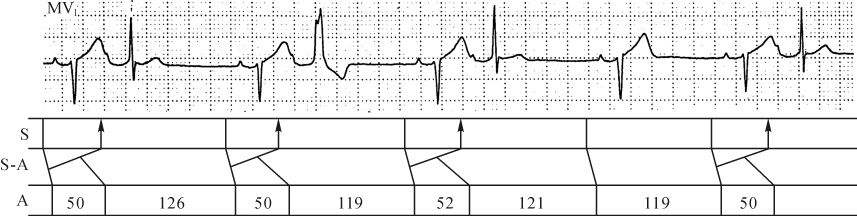
\includegraphics[width=3.25in,height=1.66667in]{./images/Image00027.jpg}
\end{table}

\subsubsection{诊断注意事项}

对所有一过性意识丧失患者必须进行全面仔细的评估,包括病史和检查。要顺序确认:是否晕厥,晕厥的原因,死亡和其他风险。尽管从死亡率角度来说,晕厥常常是良性的,但仅仅确定患者是低死亡风险患者是不够的,因为晕厥常常会复发,增加外伤风险,并且影响生活质量和正常工作。晕厥的诊断和治疗是富于挑战性的。首先,晕厥仅仅是一过性意识丧失众多原因中的一种;其次,患者症状短暂,就诊时一般都已完全恢复,并且有价值的查体发现很少;第三,自发的临床事件很少被医学专业人员目击,临床事件的病史经常是来自“二手”甚至“三手”的资讯。急诊科医生应仔细考虑所发现的异常是否和临床情况相匹配,强调长程监测的重要性。为了使患者得到准确的预后评估和治疗选择,强调应尽可能确定患者的病因。

\subsection{治疗}

\subsubsection{晕厥治疗的一般原则}

晕厥治疗的一般原则是:延长生命、预防复发、防治躯体损伤。

采取基础预防性治疗还是加强治疗取决于下列临床情况:①晕厥的病因。②晕厥复发的可能性大小。③晕厥的死亡危险性大小,主要取决于心脏病和血管病的性质和严重程度。④复发次数或晕厥导致躯体或精神伤害的危险性大小。⑤发生晕厥可能对个人职业或业余爱好造成的影响(如个人经济和生活方式问题)。⑥对公共健康的危险性如汽车司机、飞行员等。⑦对治疗有效性、安全性和不良反应的评估(特别要考虑患者的伴随疾病)。根据晕厥不同病因和机制以及危险分层,采取不同的治疗策略。晕厥的治疗流程见图\ref{fig4-2}。

\subparagraph{反射性晕厥的治疗}

反射性晕厥包括血管迷走神经性晕厥、颈动脉窦综合征(CCS)和情景性晕厥,其治疗目标首先是预防症状复发和晕厥相关的损伤,改善生活质量。自2004年指南发表后,治疗方面最大的进展是在生活方式方面上,反射性晕厥非药物治疗的基石是教育,让患者相信这是一种良性情况。一般来讲,最初的治疗涉及让患者了解这一疾病及如何避免诱因(如闷热而拥挤的环境,血容量不足)等相关方面的教育。早期识别前驱症状,采取某些动作以终止发作{[}如仰卧位,身体反压调整(PCMs){]}。避免引起血压降低的药物(包括α受体阻滞剂、利尿剂和酒精)。对于不可预测的频繁发作的晕厥需给予其他治疗。特别是:①非常频繁发作影响到生活质量;②反复晕厥没有或仅有非常短时的晕厥先兆,但患者暴露于有外伤危险的情况下;③晕厥发生在高危作业时(如驾驶、操作机器、飞行、竞技性体育运动等)。

具体治疗方法如下:①身体反压调整(PCMs):非药物的物理治疗,为反射性晕厥的一线治疗。PCMs即双腿肌肉等长收缩PCMs(双腿交叉),或双上肢肌肉等长收缩PCMs(双手紧握和上肢紧绷),多中心前瞻性研究显示,使用这种方法,在反射性晕厥发作时能够显著升高血压,多数情况下可使患者避免或延迟意识丧失。②倾斜训练:可能会减少晕厥复发,但是患者依从性较差,治疗受到影响。③药物治疗:许多试图用于治疗反射性晕厥的药物结果都令人失望。这些药物包括β受体阻滞剂、丙吡胺、东莨菪碱、茶碱、麻黄碱、依替福林、米多君、可乐定和5-羟色胺重吸收抑制剂。由于在反射性晕厥时外周血管常常不能得到适当的收缩,α受体激动血管收缩剂(依替福林和米多君)曾被使用,但是,治疗效果不一致。专家组认为,反射性晕厥患者长期单独使用α受体激动剂药物治疗可能有一些作用,对于偶发患者不建议长期治疗。在长时间站立或从事常常诱发晕厥的活动前1小时服用单剂量的药物避免晕厥发生,对有些患者可能有用。④心脏起搏:起搏治疗反射性晕厥的随机对照试验得出了相反的结果。专家组认为在迷走神经性晕厥中血管减压部分通常起主要作用,所以得出起搏欠佳的结果并不奇怪。而颈动脉窦晕厥心脏起搏治疗可能有效,双腔起搏一般优于单腔心室起搏。反射性晕厥治疗的建议见表\ref{tab4-11}。

\begin{figure}[!htbp]
 \centering
 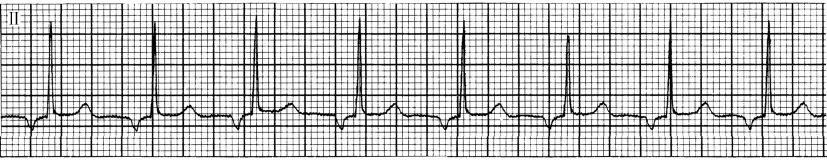
\includegraphics[width=4.82292in,height=2.16667in]{./images/Image00028.jpg}
 \captionsetup{justification=centering}
 \caption{晕厥的治疗流程}
 \label{fig4-2}
  \end{figure} 

\begin{table}[htbp]
\centering
\caption{反射性晕厥的治疗建议}
\label{tab4-11}
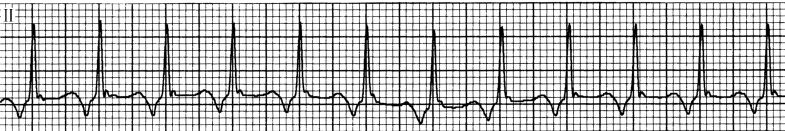
\includegraphics[width=3.28125in,height=3.66667in]{./images/Image00029.jpg}
\end{table}

注:CSS =颈动脉窦综合征;VVS =血管迷走晕厥

\subparagraph{直立性低血压的治疗}

治疗目标是预防症状复发以及晕厥造成的伤害,改善生活质量。药物诱发的自主神经功能失调可能是直立性低血压性晕厥最常见的原因,主要治疗方法是停药,仅有少数患者由于病情不能停药。引起直立性低血压最常见的药物是利尿剂和血管扩张剂,酒精也是常见的原因,其除诱发自主神经性晕厥外还可引起躯体神经系统疾病。包括对中枢神经系统的直接作用和血容量不足。主要治疗是戒酒。对于原发性和继发性自主神经功能失调的患者,了解血压调节的生理和病生理机制十分重要,治疗的主要目标是改善由于脑灌注不足导致的症状(如晕厥、先兆晕厥、意识模糊等)。尽管通过上述治疗使收缩压升高幅度不大(10~15mmHg),但可以明显改善直立性低血压的症状;使平均动脉压升高恰到好处,重新达到自主神经的调节范围内,进而可以明显改善神经调节功能。应对所有患者进行健康教育,使他们了解影响血压的因素,避免突然站起(尤其是醒后)、长时间站立、白天长时间卧位休息、用力排尿排便、过度通气、高温环境(包括热澡水、淋浴、桑拿浴)、极度用力、暴食(特别是精制的碳水化合物)、具有扩血管作用的酒精和药物。动态监测血压有助于了解白天不同环境中的血压变化,了解高血压患者药物对卧位/夜间血压的影响。扩张细胞外容量是重要的治疗目标。对无高血压的患者,应指导摄入足够的盐和水。每天达到2~3L液体和10g氯化钠。快速摄入冷开水对运动中或餐后低血压者有明显疗效;高枕位睡眠(头部抬高10°)可防止夜间多尿,维持适量的体液量及改善夜间高血压。老年患者可佩戴腹带或加压弹力袜以减轻下肢血液蓄积;有先兆晕厥时可采取交叉腿和蹲位姿势等预防措施。α受体激动剂(米多君)是慢性自主神经异常者的首选药物。氟氢可的松(0.1~0.3mg/d)可促进钠水潴留及扩张血容量,改善晕厥症状。其他治疗如去氨加压素用于伴夜尿增多者;奥曲肽用于餐后低血压,促红细胞生成素用于贫血者等。直立性低血压治疗建议见表\ref{tab4-12}。

\begin{table}[htbp]
\centering
\caption{直立性低血压的治疗建议}
\label{tab4-12}
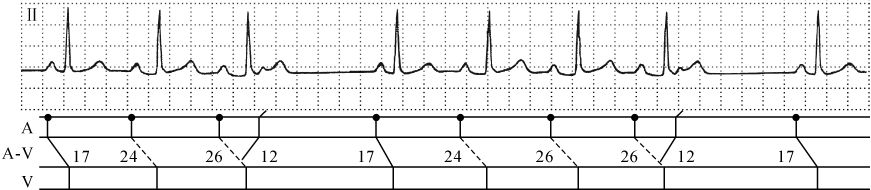
\includegraphics[width=3.27083in,height=2in]{./images/Image00030.jpg}
\end{table}

\subparagraph{心律失常性晕厥的治疗}

治疗目标预防症状复发,改善生活质量,减低死亡危险。原发性心律失常与心脏本身疾病或解剖异常有关,是最常见晕厥原因之一。包括原发性窦房结功能异常(缓慢、快速心律失常)、传导系统病变、室上性心动过速和室性心动过速。这种晕厥的基础是多方面的,包括心律失常的频率、左心室的功能状态和血管的代偿作用(包括神经反射作用)。

\hypertarget{text00014.htmlux5cux23CHP1-4-4-1-3-1}{}
(1) 窦房结功能不全:

窦房结功能不全伴缓慢心律失常、或SNRT异常引起的晕厥,起搏治疗效果显著。永久起搏可明显缓解症状,但对生存率无影响。预防晕厥复发的另一主要措施是停用加重或诱发心动过缓的药物,如无合适的替代药物应行心脏起搏。

\hypertarget{text00014.htmlux5cux23CHP1-4-4-1-3-2}{}
(2) 房室传导系统疾病:

AV阻滞引起的晕厥需起搏治疗,永久右室心尖部起搏的危害已获证实,但其替代起搏位点仍有争议。AV阻滞伴LVEF下降、心力衰竭(心衰)及QRS间期延长所致者可考虑双腔起搏。

\hypertarget{text00014.htmlux5cux23CHP1-4-4-1-3-3}{}
(3) 阵发性室上性和室性心动过速:

阵发性室上性和室速或典型心房扑动引起的晕厥,应首选导管消融术。尖端扭转型室速所致的晕厥主因是应用引起QT间期延长的药物所致,应立即停药。心功能正常或轻度受损者,如出现室速伴晕厥,可考虑导管消融或药物治疗。心功能不全、室速或心室颤动伴晕厥且病因无法祛除者应植入埋藏式心脏复律除颤器(ICD)。ICD虽不能有效预防晕厥复发,但可降低猝死风险。心律失常性晕厥的治疗见表\ref{tab4-13}。

\subparagraph{SCD高危患者不明原因晕厥的治疗}

其治疗目标不仅仅是防止晕厥再发,而且要治疗基础疾病和减少SCD的风险。严重主动脉狭窄或心房黏液瘤所致的晕厥可考虑手术治疗;继发于急性心血管事件如肺栓塞、心肌梗死或心包压塞者主要针对病因治疗;大多数心肌缺血所致者可采用药物和(或)血管重建;由原发性肺动脉高压或限制性心肌病引起者,一般不易纠正原发病。急、慢性冠状动脉疾病或LVEF下降均可增加死亡风险,故需评估缺血的严重程度,且如果有适应证应考虑血运重建。但血运重建并不能改善恶性心律失常引起的不良后果,因此该类患者应行电生理检查以评估有无心律失常。心衰且符合最新指南制定的ICD适应证者,无论晕厥发生机制是否明确,均应植入ICD。有研究显示,植入ICD的晕厥患者生存率明显增加;不明原因晕厥的缺血性或非缺血性心肌病伴心衰或LVEF严重下降者应植入ICD(Ⅰ类,A级);LVEF正常和电生理检查阴性者不建议植入ICD。其他类型心脏病:①肥厚性心肌病伴不明原因晕厥尤其是发作间期短(<
6个月)、相对危险度>
5的患者,其猝死风险较高;植入ICD效果明显。②约1/3致心律失常性右室心肌病(ARVC)者会发生晕厥。年轻、严重右室发育不全、左室功能障碍、多形性室速、心室晚电位、epsilon波及有猝死家族史者,如无其他病因应考虑植入ICD。③遗传性离子通道异常性心脏病常以晕厥为先兆表现,但该类患者是否应植入ICD仍有争议。SCD高危晕厥患者ICD适应证见表\ref{tab4-14}。

\begin{table}[htbp]
\centering
\caption{心律失常性晕厥的治疗建议}
\label{tab4-13}
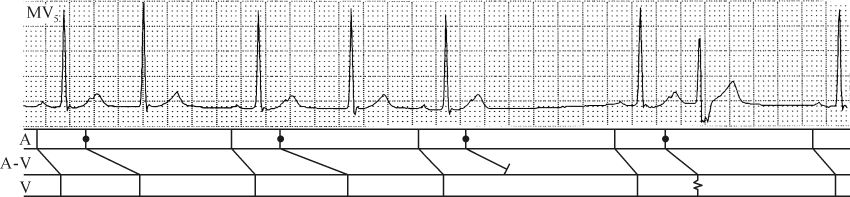
\includegraphics[width=3.29167in,height=7.86458in]{./images/Image00031.jpg}
\end{table}

\begin{table}[htbp]
\centering
\caption{SCD高危晕厥患者ICD适应证}
\label{tab4-14}
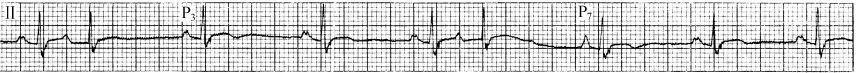
\includegraphics[width=3.3125in,height=3.55208in]{./images/Image00032.jpg}
\end{table}

\subparagraph{特殊人群晕厥的处理}

\hypertarget{text00014.htmlux5cux23CHP1-4-4-1-5-1}{}
(1) 老年人晕厥:

老年人最常见的晕厥原因是OH、反射性晕厥,特别是颈动脉窦过敏和心律失常。一个患者可能有不同的机制共同作用,从而给诊断带来困难。与OH相关的住院治疗随着年龄的增加而增加,65~74岁是4.2\%,75岁以上为30.5\%。在有晕厥症状的患者之中,25\%是年龄相关的OH;其他OH主要是药物和特发性或继发性房颤所致。有OH的老年患者常有卧位收缩期高血压,并在接受多种药物治疗,给予OH药物治疗会加重卧位高血压,反之亦然。心脏抑制型颈动脉窦过敏是晕厥的原因,老年者高达20\%。血管减压型为主的颈动脉窦敏感同样常见,但是其在晕厥中的作用知之甚少。

对于老年人诊断检查和策略应注意:①老年人的OH常常具有重复性(特别是与药物或年龄相关)。因此,应反复进行OH评价,最好在早晨和(或)晕厥刚刚发生后进行。②对没有晕厥史者,即使颈动脉窦过敏不具特异性,颈动脉窦按摩检查也是特别重要的。③评价老年人反射性晕厥时,倾斜试验耐受性和安全性均很好。其阳性率与年轻人相仿,特别是在硝酸甘油激发后。④如果怀疑血压不稳定(如服药后或者餐后),24小时动态血压监测可能有帮助。⑤由于老年人心律失常发生频率高,对不明原因晕厥的老年人ILR特别有用。

\hypertarget{text00014.htmlux5cux23CHP1-4-4-1-5-2}{}
(2) 儿童晕厥:

对儿童晕厥的诊断评估与成人类似。反射性晕厥占病因学的绝大部分。但是在少数情况下,晕厥的发生是威胁生命的心律失常或心脏器质性异常所致。晕厥应该与癫痫和精神性假性晕厥鉴别,后者十分少见,但是是儿童TLOC的重要原因。

在幼童时期的两种特殊情况:①婴儿反射性晕厥发作(也叫做苍白屏气发作或反射性缺氧发作)是由短暂不愉快刺激导致的由迷走神经介导的心脏抑制所致。②窒息低氧性TLOC(发绀性呼吸停止)以哭闹时呼吸运动终止于呼气阶段为特征,从而导致发绀和通常所见的TLOC。

儿童倾斜试验的假阳性和假阴性率均较高,因此对于反射性晕厥的初步评估应持审慎态度。有报道对于健康少年儿童在静脉用药后进行倾斜试验时,先兆晕厥的比率非常高(40\%)。年轻患者首发晕厥可能为少见的、但是是威胁生命的疾病,如LQTS、Kearns-Sayre综合征(外眼肌麻痹和进行性心脏传导阻滞)、Brugada综合征、儿茶酚胺依赖性多形性VT、预激综合征、ARVC、肥厚型心肌病、肺动脉高压、心肌炎、先天性心脏病修补术后心律失常、冠状动脉异常起源。

对于具有下面情况的患儿可能提示有心脏性病因,应迅速进行心脏方面的评估:①家族史:年轻的SCD者<
30岁;家族性心脏病。②已知或可疑心脏病。③触发事件:噪音、惊吓、极端情感刺激。④运动时晕厥,包括游泳。⑤仰卧或者睡眠时无晕厥先兆,或晕厥前有胸痛或心悸。

儿童晕厥的治疗策略与成人相同。然而需要强调的是目前缺乏关于儿童反复晕厥良好设计的研究,因此药物和倾斜训练的有效性不能肯定。此外,尽管有血管迷走神经性晕厥以及长时间心脏停搏的证据,由于为一过性和良性晕厥,因此应避免安装起搏器。

总之,对儿童晕厥评估要点有几方面:①儿童期晕厥常见,绝大部分源于反射机制,很少部分是源于威胁生命的病因所致。②对良性和严重病因的鉴别主要依靠病史、体格检查和心电图。③对反射性晕厥年幼患者的治疗基石是教育并使之放心。

\hypertarget{text00014.htmlux5cux23CHP1-4-4-1-5-3}{}
(3) 驾车与晕厥:

随着轿车进入中国普通家庭,驾车与晕厥的问题显得重要起来。但是,调查显示,在有晕厥病史的患者中,交通事故的发生率低于普通人群。晕厥患者驾驶的建议见表\ref{tab4-15}。

\begin{table}[htbp]
\centering
\caption{晕厥患者驾驶的建议}
\label{tab4-15}
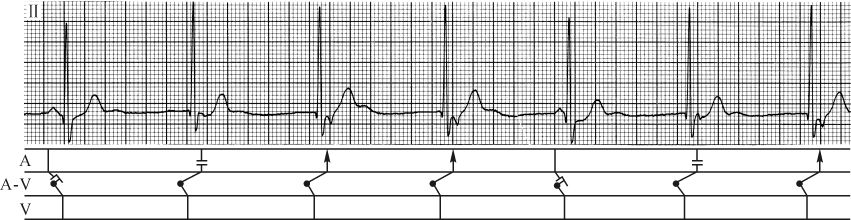
\includegraphics[width=3.27083in,height=2.86458in]{./images/Image00033.jpg}
\end{table}

注:第一组(私人驾驶者):驾驶摩托,小汽车或其他小型车辆,没有拖车;第二组(职业驾驶者):驾驶3.5吨以上汽车,除驾驶员外8座以上客车;出租车,救护车,介于私人与职业间车辆以及地方法规规定的车辆;

*:神经介导的晕厥严重且发作频繁,或正在从事高危活动;或者是复发或不可预测的高危患者

\subsection{预后}

晕厥的预后主要取决于两方面:①死亡风险及致命性事件:器质性心脏病及原发性电生理疾病是心源性猝死及晕厥患者总体死亡率的高危因素;合并联合病变的直立性低血压患者与普通人群相比,其死亡风险增加2倍;年轻且无器质性或电生理异常性心脏病的反射性晕厥患者,预后较好。大多数预后不良或死亡的患者多与基础疾病而非晕厥本身的严重程度有关。②晕厥复发及其危害:晕厥发生的次数是预测其复发的最佳指标,如诊断不明、低风险及年龄>
40岁、曾有1~2次晕厥发作史者,其复发率分别为15\%(1年内)和20\%(2年内);有3次发作史者,其复发率分别为36\%(1年内)和42\%(2年内)。


\hypertarget{text00015.htmlux5cux23CHP1-4-6}{}
参 考 文 献

Moya A,Sutton R,Ammimti F,et al. Guidelines for the diagnosis and
management of syncope(version 2009):the Task Force for the Diagnosis
and Management of Syncope of the European Society of
Cardiology(ESC).Eur Heart J,2009,30:2631-2671.

\protect\hypertarget{text00016.html}{}{}

\chapter{抽搐与惊厥}

抽搐(tics)系指全身或局部骨骼肌群非自主抽动或强烈收缩。抽搐包括痫性发作(seizure)和非痫性发作。痫性发作是脑神经元突然过度放电引起的短暂脑功能失调,患者出现全身(四肢、躯干、颜面)骨骼肌非自主强直性(持续肌肉收缩)与阵挛性(断续肌肉收缩)抽搐,引起关节运动和强直,又称癫痫发作。全面性强直-阵挛性抽搐即为惊厥发作(convulsion),常为全身性、对称性,多伴有意识障碍。

癫痫(epilepsy)则特指慢性反复发作性短暂脑功能失调综合征,具有反复性和发作性两个基本特征。癫痫持续状态(status
epilepticus)是抽搐患者最严重的表现形式之一,是指一次癫痫发作持续时间较久(>
30分钟),或癫痫频繁发作,发作间歇期意识尚未完全恢复。但研究显示较短暂的癫痫发作(<
30分钟)也可导致神经功能受损,且一旦痫性发作超过5分钟,自发终止的可能性就不大,所以建议在急诊情况下如癫痫发作超过5分钟即考虑癫痫持续状态。快速评估和控制癫痫发作是本章讨论的重点,从气道保护、神经功能稳定和寻找可能病因等三个方面积极应对,以减少其致残和死亡率。

\subsection{病因与发病机制}

抽搐的表现形式多样,主要分痫性发作和非痫性发作,前者有惊厥(全面性强直-阵挛发作)、强直性抽搐、肌阵挛发作、失神发作、自动症(automatism)等,后者见于低血钙手足抽搦、假性癫痫发作(如癔症性抽搐)等,因此其病因和发病机制非常复杂。

\subsubsection{病因}

\subparagraph{癫痫和癫痫综合征}

具有特征性临床症状和脑电异常,但病因不清楚的癫痫发作,临床上倾向于基因突变和某些先天性因素所致,有明显遗传倾向;在患者神经系统中目前尚未发现有足以引起人类癫痫发作的器质性损伤或生化异常。

\subparagraph{症状性癫痫}

各种明确或可能的中枢神经系统病变所致,如脑外伤、围产期损伤、脑血管病、肿瘤、中枢神经系统感染、寄生虫、遗传代谢性疾病(如低血糖)、神经系统变应性疾病、狼疮脑病等。

\subparagraph{状态关联性癫痫发作}

患者癫痫发作与一些特殊状态有关,如高热、缺氧、内分泌和电解质异常(低血糖、低钠血症、高渗透压、尿毒症、肝功能衰竭)、药物与毒物、酒精和阿片类物质戒断、过度饮水、睡眠剥夺等。正常人(脑结构和功能正常)在上述特殊状态下也可出现癫痫发作,但一旦去除相关状态即不再出现癫痫发作。

\subparagraph{隐源性癫痫发作}

临床表现提示症状性癫痫发作,但无特定的临床和脑电图特征,也未找到明确的病因。

上面所列主要是痫性发作抽搐的病因分类,为避免分类混乱,尚未包括非痫性发作抽搐相关病因。另外还要注意抽搐与晕厥、过度通气综合征、偏头痛、发作性睡病及各种不自主动作(如震颤、舞蹈动作、手足徐动、扭转痉挛、肌痉挛等)间的鉴别。

\subsubsection{发病机制}

抽搐的发生机制极为复杂,至今仍未阐明。目前脑组织的生理、生化方面的研究显示,抽搐发作主要机制是由大脑运动神经元的异常放电致脑功能短暂失调。该异常放电主要是神经元膜电位的不稳定引起,可由代谢、营养、皮质病变等激发,并与遗传、免疫、精神因素及微量元素等有关。具体来说,根据引起肌肉异常收缩的电兴奋信号的来源不同,可分为以下两类机制:

\subparagraph{大脑功能的短暂性失调}

这是脑内神经元过度同步化放电的结果,当异常的电兴奋信号传至肌肉时,则引起广泛肌群的强烈收缩而形成抽搐。在正常情况下,脑内对神经元的过度放电及由此形成过度同步化,均有一定控制作用,即构成所谓抽搐阈。许多脑部病变或全身性疾病可通过破坏脑的控制作用,使抽搐阈下降,甚至引起抽搐。①神经元异常放电及其扩布:颅内外许多疾病,可通过不同途径影响膜电位的稳定,有直接引起膜电位降低(如低钠血症),使神经元更易去极化而产生动作电位(兴奋阈下降);间接通过影响能量代谢或能量缺乏,导致膜电位下降;神经元膜的通透性增高,使细胞外钠流入细胞内,而细胞内钾外流,因而膜电位及兴奋阈降低。②神经递质与突触传递的改变:中枢神经系统某些神经元的轴突于突触点释放抑制性递质,对神经元的过度放电及同步化也起一定控制作用。当兴奋性神经递质过多(如有机磷中毒时乙酰胆碱积聚过多)或抑制性神经递质过少(如维生素B\textsubscript{6}
缺乏时,由于谷氨酸脱羧酶的辅酶缺乏使谷氨酸转化成抑制性递质的γ-氨基丁酸减少)均可导致抽搐。③抑制系统通路受阻断:脑内有些神经元组成广泛的抑制系统,有控制神经元过度放电的作用。脑部病变除了直接损害神经元膜或通过影响脑血液供应外,也可能阻断抑制系统,使神经元容易过度兴奋。④网状结构的促去同化系统功能降低:脑干神经元放电同步化系统与网状结构的促去同化系统之间的平衡,对控制神经元的过度放电及同步化起相当的作用。

\subparagraph{非大脑功能的障碍}

引起肌肉异常收缩的电兴奋信号来源于下运动神经元,主要是脊髓的运动神经元或周围运动神经元。如破伤风杆菌外毒素选择性作用于中枢神经系统(主要是脊髓、脑干的下运动神经元)的突触,使其肿胀而发生功能障碍;马钱子碱中毒引起脊髓前角细胞过度兴奋,发生类似破伤风的抽搐;各种原因的低钙血症,除了使神经元膜通透性增高外,也常由于下运动神经元的轴突(周围神经)和肌膜对钠离子的通透性增加而兴奋性升高,引起手足搐搦。

\subsubsection{儿童惊厥发病机制}

儿童惊厥(6岁以下)发生率是成人的10~15倍,儿童惊厥的发病机制有其特殊性。婴幼儿大脑皮质功能未完善/抑制差、兴奋易扩散、神经髓鞘未完全形成、神经传导分化不全、冲动易泛化、血-脑脊液屏障不良、毒物易渗入脑组织及水电解质代谢不稳定等因素是导致儿童惊厥高发生率的主要原因。相对成人而言,短暂性脑功能失调对小儿神经系统发育影响更大,一次惊厥对近记忆的一过性影响与脑震荡所致的损伤相当,而惊厥持续状态可产生严重不可逆脑损伤,小儿惊厥30分钟以上就可产生神经元缺血病变,影响小儿智力和健康。通常成人惊厥超过6小时才产生类似变化。

\subsection{诊断思路}

抽搐并不是单一疾病,而是许多疾病的严重临床表现或主要征象。因此,在诊断过程中,应综合分析各方面资料,才能明确其发生的原因。

\subsubsection{抽搐的诊断}

\hypertarget{text00016.htmlux5cux23CHP1-5-2-1-1}{}
(一) 病史

不同疾病所致的抽搐 ,其临床表现不尽相同,故详细收集病史是非常重要的。

\subparagraph{明确抽搐类型}

依抽搐的形式,可分为以下两种:①痫性发作(癫痫发作);②非痫性发作。前者(尤其是全面性强直-阵挛发作,即惊厥发作)需要急诊医师快速评估和保护气道、控制癫痫发作,并积极寻找病因。而非痫性发作抽搐虽然不似前者致命,但抽搐的控制更加困难,临床重点是寻找可能病因。判断癫痫发作最重要的依据是患者的病史,如先兆症状、发作时状态及发作后意识模糊等,而不是依靠神经系统查体和实验室检查。患者发作后意识模糊状态高度提示癫痫发作。

\subparagraph{了解基础疾病和用药史}

对诊断有重要参考价值。如反复发作常提示癫痫,新近发生的癫痫发作通常由于原发性神经疾病和系统性疾病或代谢紊乱所致,有外伤、感染以及内脏器官基础疾病史者提示可能为症状性癫痫。还须详细了解用药史和饮酒史,尤其是抗癫痫药物使用情况。

\subparagraph{伴随症状}

对病因诊断有相当意义。

\hypertarget{text00016.htmlux5cux23CHP1-5-2-1-1-3-1}{}
(1) 症状性癫痫发作:

①颅内疾病时可伴有头痛、发热等;②阿-斯综合征抽搐时伴有心搏停止、心音及脉搏消失;③低血糖所致抽搐前多有乏力、饥饿、出汗,发作时伴有心动过速、血压升高、瞳孔散大;④子痫者伴有头痛、眼花、呕吐,可有高血压、水肿和蛋白尿;⑤嗜铬细胞瘤时伴有心跳快、气促、出汗、面色及四肢苍白、发冷、头痛、血压急剧升高、瞳孔散大;⑥尿毒症患者伴有氮质血症和酸中毒表现。

\hypertarget{text00016.htmlux5cux23CHP1-5-2-1-1-3-2}{}
(2) 低血钙性手足搐搦症:

①甲状旁腺功能减退症患者可伴有哮喘,易激动、焦虑等精神症状,皮肤粗糙,头发脱落,牙齿发育不良;②肠源性手足搐搦症患者伴有慢性腹泻;③肾病性手足搐搦症患者伴有代谢性酸中毒表现;④假性甲状旁腺功能减退症患者伴有先天畸形如矮胖、圆脸、短指。

\hypertarget{text00016.htmlux5cux23CHP1-5-2-1-1-3-3}{}
(3) 血钙正常性碱中毒性手足搐搦症:

伴有引起碱中毒的症状,如过度换气,大量呕吐或服用大量碱性药物。

\hypertarget{text00016.htmlux5cux23CHP1-5-2-1-2}{}
(二) 体格检查

导致抽搐病因众多 ,常涉及临床各科,详细系统地体检十分重要。通常包括:

\subparagraph{系统查体}

重点是生命体征和有无创伤表现。但几乎体内各重要内脏器官的疾病均可引起抽搐,故须按系统进行检查。如心音及脉搏消失、血压下降或测不到,或严重心律失常,要考虑心源性抽搐;苦笑面容、牙关紧闭、角弓反张者要考虑破伤风;怀疑手足抽搦症时要查:①Chvostek征:以中指轻扣耳前面神经,可引起同侧面肌抽搐;②Trousseau征:以血压计袖带缠绕一侧上臂,打气至舒张压与收缩压之间,维持3分钟,可引起该侧手的搐搦。

\subparagraph{神经和精神科查体}

有助于致抽搐病变的定性与定位。重点注意瞳孔反射、病理征、局灶神经体征、眼底情况。

\hypertarget{text00016.htmlux5cux23CHP1-5-2-1-3}{}
(三) 辅助检查

根据病史
、体检所提供的线索,选择辅助检查项目。①全身性疾病:应选择相应的检查。除了血尿粪常规外,有心电图、血液生化(血糖、尿素氮、电解质等)、血气分析、肝肾功能、内分泌功能测定、毒物分析等。②神经系统疾病:根据临床提示的病变部位和性质,选择相应的辅助检查。如脑电图、肌电图、脑脊液、神经影像学检查(头颅CT、MRI、MRA)等,近年来PET等功能影像学检查手段越来越多地被用于抽搐的病因诊断,它可实现脑局部代谢变化,辅助癫痫灶定位。

\subsubsection{抽搐的病因判断}

所有抽搐患者均应结合上述资料尽可能做出病因诊断,如为首次发作,首先须排除各种疾病引起的症状性发作,寻找可逆因素(如低血糖、低钠血症、低钙血症、药物过量等)。临床上还可根据抽搐时是否伴有意识障碍,可将抽搐分为两大类:

\hypertarget{text00016.htmlux5cux23CHP1-5-2-2-1}{}
(一) 伴意识障碍性抽搐

\subparagraph{大脑器质性损害性抽搐}

其特点为:①抽搐为阵挛性和(或)强直性;②意识障碍较重,持续时间长,且多伴有瞳孔散大、大小便失禁、面色青紫等表现,多数有颅内高压表现;③脑脊液检查常有异常发现,脑电图、CT、MRI等检查有助于诊断。

\subparagraph{大脑非器质性损害性抽搐}

其特点有:①意识障碍可轻可重,多数为短暂性昏迷,约在数秒至数十秒内自行恢复;②全身性疾病的表现往往比神经系统表现更明显;③无明确的神经系统定位体征;④脑脊液检查和脑电图检查多正常。

\hypertarget{text00016.htmlux5cux23CHP1-5-2-2-2}{}
(二) 不伴意识障碍性抽搐

可分为神经肌肉兴奋性增加(见于低血钙或低血镁、破伤风或马钱子碱中毒)和神经肌肉兴奋性正常(见于药物戒断反应、癔症性抽搐)两类,但以电解质紊乱(如低血钙、低血镁等)所致者较为常见。此类抽搐的特点是呈疼痛性、紧张性肌收缩,常伴有感觉异常。根据病史和临床表现常可确定这类抽搐的病因。如诊断有困难时,可测定血钙与血镁。在紧急情况下,可先静注10\%葡萄糖酸钙10ml,无效时可再静注25\%硫酸镁5~10ml。这样既有鉴别诊断的意义,又有治疗作用。

\subsubsection{临床常见抽搐}

\subparagraph{癫痫发作(痫性发作)}

患者出现全身骨骼肌非自主强直性与阵挛性抽搐,引起关节运动和强直,伴或不伴意识障碍。根据临床表现可分为:①部分发作(局灶发作):单纯部分性发作(发作时无意识障碍)、复杂部分性发作(有不同程度意识障碍);②全面性发作:全面性强直-阵挛发作(即癫痫大发作,俗称惊厥,部分患者发作前有先兆,分强直期、阵挛期和痉挛后期)、强直性发作、阵挛性发作、肌阵挛发作、失神发作、失张力性发作等。

分类颇显繁杂,急诊临床重点是识别:是否是癫痫发作?是全面性发作吗?是癫痫持续状态吗?由于癫痫持续状态期间脑神经元能耗骤增,脑内pH下降,加之全身性缺氧,肌肉强烈而持久性收缩,酸性代谢产物增加,可导致脑缺氧、脑水肿甚至脑疝形成。持续状态时需要紧急保护气道、控制癫痫发作(稳定神经功能)和确定病因。

\subparagraph{手足搐搦症}

以疼痛性、紧张性肌肉收缩为特征,多伴有感觉异常,见于各种原因所致的低钙血症和低镁血症。表现为间歇发生的双侧强直性痉挛,上肢较显著,尤其是在手部肌肉,呈典型的:“助产手”,即手指伸直内收,拇指对掌内收,掌指关节和腕部屈曲;常有肘伸直和外旋。下肢受累时,呈现足趾和踝部屈曲,膝伸直。严重时可有口、眼轮匝肌的痉挛。发作时意识清,Chvostek征和Trousseau征阳性。

\subparagraph{破伤风}

破伤风杆菌外毒素-破伤风痉挛毒素可阻断脊髓的抑制反射,脊髓前角运动神经元兴奋性增高,同时也使脑干广泛脱抑,导致肌痉挛、肌强直,表现为张口困难、牙关紧闭、腹肌僵硬、角弓反张。肌强直的特点是在抽搐间歇期仍存在,肌抽搐可为自发性,亦可因外界刺激而引起,面肌强直和痉挛形成苦笑面容,咽肌和膈肌受累导致饮水困难和呛咳。破伤风的抽搐虽可十分严重,但神志清楚。外伤史有助于疾病的诊断。

\subparagraph{癔症性抽搐}

属一种功能性动作异常。患者多为年轻女性,在精神因素刺激下发作,表现为突然倒下,全身僵直、牙关紧闭、双手握拳,其后不规则的手足舞动,常杂以捶胸顿足、哭笑叫骂等情感反应,发作持续数分钟至数小时。其特点是:①抽搐动作杂乱,无规律可循,不指向神经系统的某一定位损害;②无瞳孔变化和病理反射;③常伴有流泪、过度呼吸、眼活动频繁和眨眼过度;④无舌头损伤及大小便失禁;⑤发作时脑电图正常;⑥暗示或强刺激可终止其发作。

\subparagraph{发热惊厥}

惊厥发作的典型临床表现是意识突然丧失,同时急骤发生全身性或局限性、强直性或阵挛性面部、四肢肌肉抽搐,多伴有双眼上翻、凝视或斜视。最常见于幼儿,发病多在6个月至6岁之间,以3岁以前小儿多见。最常见于上呼吸道感染、扁桃腺炎,少数见于消化道感染或出疹性疾病,约一半患儿有家族史,提示同遗传因素有关。惊厥的发生常与发热相关,但热度高低并不与之呈正相关。发作形式多为单次,全身性强直、阵挛性发作,持续时间在30秒钟以内,一般不超过10分钟,脑电图有节律变慢或枕区高幅慢波,在退热后1周内消失。可能每年有一至数次同样发作,但若无脑损害征象,并不导致癫痫。

\subparagraph{中毒性抽搐}

最常见于急性中毒。其发生抽搐的主要机制:①直接作用于脑或脊髓,使神经元的兴奋性增高而发生抽搐。大多是药物的过量,如戊四氮、贝美格(美解眠)、樟脑、印防己毒素、阿托品、麦角胺、丙米嗪、氯丙嗪、白果等;②中毒后缺氧或毒物作用,引起脑代谢及血循环障碍,形成脑水肿。见于各种重金属、有机化合物、某些药物和食物的急性重度中毒。临床多呈全身性肌强直阵挛性发作,少数也可呈局限性抽搐,有的可发展为癫痫状态。常合并其他中毒表现。马钱子碱(士的宁)中毒的临床表现类似破伤风,仅在抽搐间隙无持续性的肌痉挛。

\subparagraph{心源性抽搐}

是指各种原因引起心排出量锐减或心脏停搏,使脑供血短期内急剧下降所致的突然意识丧失及抽搐,也称昏厥性抽搐。常见于严重心律失常、心排血受阻的心脏病或某些先天性心脏病、心肌缺血、颈动脉窦过敏、血管抑制性昏厥、直立性低血压等。其抽搐时间多在10秒钟内,较少超过15秒钟,先有强直,躯体后仰,双手握拳,接着双上肢至面部阵挛性痉挛,伴有意识丧失,瞳孔散大、流涎,偶有大小便失禁。发作时心音及脉搏消失,血压明显下降或测不到。脑电图在抽搐时呈电位低平,其后为慢波,随意识恢复后逐渐正常。

\subparagraph{急性颅脑疾病相关抽搐}

颅内感染、颅脑损伤、急性脑血管病是导致症状性癫痫发作的主要因素。抽搐多为痫性发作,且多与病变程度相平衡,有的随着颅脑病变的加剧抽搐频繁、加剧,甚至发展为癫痫持续状态。抽搐仅是临床表现之一,大多还有脑局灶或弥散损害的征象,如头痛、呕吐、精神异常、偏瘫、失语、意识障碍、脑膜刺激征等表现。脑脊液检查及CT、MRI等检查可有相应的阳性发现。

\subparagraph{药物戒断反应}

长期连续服用安眠药,主要是巴比妥类安眠药患者,常产生药物依赖性甚至成瘾,在突然停药后可引起严重戒断反应,表现为异常兴奋,焦虑不安、躁动甚至发生四肢抽搐或强直性惊厥。阿片类药物的戒断反应较安眠药更严重而持久。处理主要是对症治疗,并逐渐停药。

\subparagraph{代谢、内分泌异常所致的抽搐}

许多代谢、内分泌疾患,可因电解质紊乱,能量供应障碍等,干扰了神经细胞膜的稳定性,而出现抽搐,同时有明显代谢、内分泌异常的临床表现。如各种疾病所致的低钙血症、低钠血症、低镁血症、碱中毒、低血糖症(血糖<
2mmol/L)等,均可致抽搐。

\subsection{处理原则}

\subsubsection{急诊处理思路}

\subparagraph{他人发现患者抽搐、晕厥、昏迷?}

急诊抽搐患者往往是被他人送来急诊就诊,而旁观者很难分别是抽搐,还是晕厥或昏迷,这时急诊医师不要仓促下结论患者是癫痫发作,具体分析思路见图\ref{fig5-1}。

\subparagraph{考虑癫痫发作的分析和处理思路}

在急诊抽搐患者处理的难点正是如何判断是否是癫痫发作,可通过以下线索来分析判断:强直-阵挛性运动病史、大小便失禁、发作后意识模糊、舌体咬伤等。在急诊如经过初始评估考虑患者为癫痫发作时,临床分析思路参考图\ref{fig5-2}。但患者的处理依然优先要考虑初始评估、稳定(保护气道)、神经功能稳定(控制癫痫发作)、寻找病因这一处理流程。

\subsubsection{保护气道}

首先应将患者置于安全处,解开衣扣,去除义齿,清除口腔异物,保持呼吸道通畅。有意识障碍者,将身体或头须转向一侧,以利口腔分泌物流出,防止吸入肺内致窒息或肺炎。分泌物较多者,准备好负压吸引器,随时吸痰。必要时给氧,气管切开或气管插管给予人工呼吸,维持正常的通气功能。

\subsubsection{快速评估和稳定}

重症病例应进行血压、心电图和脉搏氧饱和度等监测,急查血电解质和动脉血气,并予吸氧,建立静脉通路。若有异常发现,应及时处理。如给予抗抽搐药物不能终止癫痫发作,需作好气管插管准备。

低血糖是最常见引起痫性发作的代谢性因素,另一方面,要注意长时间抽搐也可致低血糖,低血糖症者,应给予50\%葡萄糖50m1,静脉推注(5分钟内);有糖尿病高血糖者,应给予胰岛素治疗。

疑有营养不良症者,应给予维生素B\textsubscript{l}
l00mg肌肉注射或静脉注射;怀疑异烟肼过量者应用维生素B\textsubscript{6}
;有低血钙症者,应给予10\%葡萄糖酸钙10ml或10\%氯化钙10m1,缓慢静脉注射(5分钟以上),必要时重复给药,但24小时给予的总钙量,一般不超过25mmol。

\begin{figure}[!htbp]
 \centering
 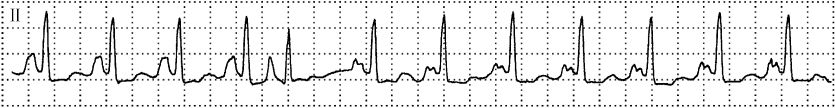
\includegraphics[width=5.88542in,height=6.04167in]{./images/Image00034.jpg}
 \captionsetup{justification=centering}
 \caption{他人发现抽搐、晕厥或昏迷患者分析思路}
 \label{fig5-1}
  \end{figure} 

\begin{figure}[!htbp]
 \centering
 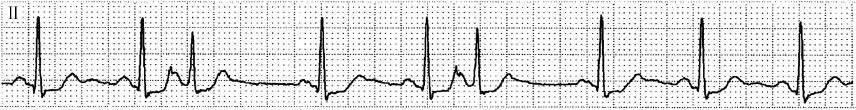
\includegraphics[width=4.77083in,height=4.34375in]{./images/Image00035.jpg}
 \captionsetup{justification=centering}
 \caption{癫痫发作的分析和处理思路}
 \label{fig5-2}
  \end{figure} 

\subsubsection{控制抽搐发作}

一旦确定是全身强直-阵挛性发作(癫痫大发作)或癫痫持续状态,及时控制抽搐是临床治疗的关键。癫痫持续状态处理流程见图\ref{fig5-3},有很强的时间紧迫性,目标是在神经功能受损前控制癫痫发作(理论上是在20分钟至1小时内控制抽搐发作)。应优先选择抗惊厥作用强、吸收快、分布半衰期长、排除半衰期短、无心肺和意识抑制作用,能肌肉注射、静脉注射和毒副作用低的药物。癫痫持续状态的药物治疗应根据患者的个体情况及时适度地应用,力争在最短的时间内终止癫痫发作,然后给予维持治疗。抽搐时切记勿强行固定四肢(否则易导致骨折、脱臼),也不要在抽搐时往患者嘴里塞牙垫、毛巾等物。抽搐停止后应加强监护,以防自伤、误伤、伤人、毁物等。

\subparagraph{地西泮(安定)}

为一线控制癫痫发作药物,适用于各年龄段。见效快,半衰期短(0.5~4小时)。成人首次剂量10~20mg,按1~5mg/min缓慢静脉注射,有效而复发者,30分钟后可重复应用,或在首次用药后将安定20~40mg加入10\%葡萄糖液100~250ml中缓慢静滴,10~20mg/h,用于维持疗效,视发作情况控制滴注速度和剂量,24小时总剂量不宜超过120mg(注:在控制癫痫发作时,地西泮剂量理论上来说没有上限)。无论地西泮的疗效如何,宜与苯妥英钠或苯巴比妥合用,预防抽搐再次发作。

儿童地西泮剂量每次0.25~0.5mg/kg静推,速度1mg/min,婴儿不超过2mg/次,幼儿不超过5mg/次。5~10岁儿童1mg/岁,儿童一次用量不超过10mg。新生儿及婴儿亦可用地西泮,每次0.5~1mg/kg肛管给药。

其他苯二氮{}
类制剂亦可选用,如劳拉西泮(氯羟安定),与地西泮相比抗惊厥作用强5倍,作用时间长3~4倍,半衰期12~16小时。静脉注射2~5mg/次(0.1mg/kg,速度2mg/min),80\%以上病例可在2~3分钟内终止发作,特别推荐在酒精戒断相关癫痫发作患者中使用。最新研究显示静脉注射劳拉西泮在控制抽搐和预防复发方面均优于地西泮。氯硝西泮抗惊厥作用是地西泮的5倍,半衰期22~32小时,静脉注射1~4mg/次,60\%病例可控制发作24小时。

如果尚未给患者建立静脉通路,地西泮可以通过直肠、气管套管内、骨髓腔内等途径给药。苯二氮{}
类药物有呼吸抑制、心动过缓和低血压、酸中毒等副作用,应用时需随时评估气道,脉搏氧饱和度降至90\%以下或呛咳作呕反射消失者,应考虑予气管插管。

\subparagraph{苯妥英钠}

控制成人癫痫发作二线治疗药物,无呼吸抑制,静脉给药能迅速达到脑内有效浓度。常用为150~250mg/次(20mg/kg),生理盐水溶解,缓慢静脉注射(1分钟小于50mg),半小时后可重复给药(100~150mg)。严重病例可加大用药剂量。儿童用量为250mg/m\textsuperscript{2}
。因为有低血压和心律失常等副作用,胃肠外给药速度不要过快,用药期间应密切观察,或行心电图和血压监测。

\subparagraph{苯巴比妥钠}

控制成人癫痫发作三线治疗药物。若足量的苯妥英钠仍不能控制抽搐发作,应立即给予苯巴比妥钠治疗。按10mg/kg静脉缓慢注射(50~100mg/min),直至发作停止,可再追加50mg,剩余部分可行肌肉注射。呼吸抑制和低血压是其常见副作用,用药前应准备气管插管和人工辅助呼吸通气。注射过程中需密切观察呼吸情况,如有抑制呼吸现象应立即停止注射,并作人工辅助通气。注意对儿童来说苯巴比妥钠是二线药物,而苯妥英钠是三线药物。

\begin{figure}[!htbp]
 \centering
 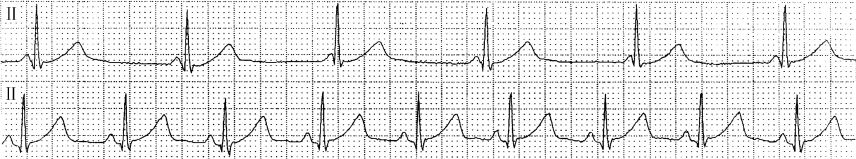
\includegraphics[width=4.11458in,height=5.28125in]{./images/Image00038.jpg}
 \captionsetup{justification=centering}
 \caption{癫痫持续状态处理路径}
 \label{fig5-3}
  \end{figure} 

(注:苯巴比妥剂量在国内有限制:一次极量为0.3g,一日极量为0.5g)

\subparagraph{其他药物}

如上述治疗无效,应考虑请神经专科医师会诊,并试用下列药物:①丙戊酸:控制癫痫发作有效药物。推荐剂量是15~20mg/kg或600~1200mg/d,分2~3次口服,其临床安全性良好,但注意在肝功能不全患者中禁用。②副醛:成人8~10ml、儿童0.3ml/kg,用植物油稀释后保留灌肠。代谢性酸中毒、肺出血、心血管抑制和直肠炎等是常见的副作用,应注意观察。③利多卡因:成人用1\%的利多卡因10ml,以20mg/min速度匀速静注。可降低心输出量,有充血性心力衰竭和肝损害减量。④10\%水合氯醛:成人20~30ml、儿童0.3ml/kg保留灌肠。

\subparagraph{全身麻醉}

处理仍无效者,可考虑收入ICU,静脉持续泵入咪达唑仑、丙泊酚等药控制癫痫发作,但其临床疗效有待进一步验证,也试用下列药物全身麻醉:①戊巴比妥:15mg/kg缓慢静脉注射,然后以0.5~1mg/(kg•h)维持。②硫喷妥钠:15mg/kg静脉缓慢推注,继以5mg/(kg•h)静脉注射维持。脑内的半衰期低于30分钟。③异戊巴比妥:200~1000mg静脉缓慢推注。

\subsubsection{病因治疗}

病因治疗是根本。如中毒性抽搐,应尽速彻底清除毒物和应用特效的解毒剂;急性感染性疾病所致者选用相应有效的抗生素,破伤风者须应用破伤风免疫球蛋白和抗生素(甲硝唑);高热惊厥,首先降温,使体温控制在38℃以下;低血糖发作应立即静注50\%葡萄糖液;水电解质平衡失调应分别纠正所缺少的钙、钠、镁;心源性抽搐者,应尽快建立有效循环,提高心排出量,治疗原发病;对肝肾功能衰竭者,改善并恢复其功能至关重要;颅内肿瘤、血肿、脓肿、脑寄生虫病及各种原因的脑水肿引起抽搐者,必须脱水降颅内压,必要时外科手术治疗。

\subsubsection{对症治疗}

癫痫持续状态l小时以上者,即有发生脑缺氧脑水肿的可能性,应酌情给予地塞米松、20\%甘露醇或利尿剂治疗,为了预防继发感染,应给予抗生素治疗。有高热者应给予降低过高体温处理。严重抽搐发作时,还可出现酸中毒、电解质紊乱、横纹肌溶解等并发症,进而又加重抽搐发作,甚至危及生命。临床上在控制癫痫发作的同时,应注意寻找并处理并发症。必须注意维持呼吸、循环、体温、水电解质平衡,保证供氧,供给充足热量,避免缺氧及缺血性脑损害。


\hypertarget{text00017.htmlux5cux23CHP1-5-4}{}
参 考 文 献

1. John Marx. Rosen's Emergency Medicine. 7th ed. Mosby,2009:113

2. Tintinalli JE. Emergency Medicine:A comprehensive study guide.6th
ed. McGraw-Hill,2004:1409

3. Rowland LP. Merritt's Neurology. 11th ed. Lippincott Williams
&Wilkins,2005:13

4. Pillow MT. Emergency Medicine. emedicine(http://emedicine.
medscape.com)updated Nov 9,2010

5. Huff JS. Emergency medicine clinics of North
America.2011,29(1):1-158

\protect\hypertarget{text00018.html}{}{}

\chapter{瘫 痪}

本章叙述的瘫痪(paralysis)是指随意肌收缩功能不全而言。其不完全障碍形成的肌力减退,属不完全性瘫痪;其完全障碍形成的随意肌收缩不能,属完全性瘫痪。本文叙述急性瘫痪的诊断与其处理原则。

\subsection{各型瘫痪的临床特征}

按病损部位不同,可将瘫痪分为肌源性、神经-肌接点性、下运动神经元性或上运动神经元性,其临床表现各具特征。现予分述如下:

\subsubsection{肌源性或神经-肌接点病损性瘫痪的临床特征}

肌源性瘫痪是指肌肉本身病变导致肌肉收缩障碍,从而引起程度不等的瘫痪而言。神经-肌接点病损性瘫痪是指神经-肌接点的递质因素或递质受体病变所引起的肌肉收缩无力而出现的瘫痪而言。

\subparagraph{瘫痪分布}

大多对称,多以肢体近端为重,不符合神经支配规律。

\subparagraph{肌束震颤}

通常没有。

\subparagraph{肌肉萎缩}

随病程进展,出现病肌萎缩,但不出现于疾病的急性期。

\subparagraph{牵张反射}

由于运动效应器病损,致紧张性牵张反射(表现为肌张力)与位相性牵张反射(表现为腱反射)均见降低。

\subparagraph{病理反射}

病理反射是上运动神经元性瘫痪的特征,因此,通常不见于肌源性或神经-肌接点病损性瘫痪。

\subparagraph{实验室检查}

肌细胞病变时出现血肌酶如肌酸磷酸激酶等升高;肌电图呈肌病性变;肌肉活检证实各种肌肉疾病的特征性改变。神经-肌接点病损性瘫痪时,通常血肌酶变动不明显,肌电图检查显示特征性改变。

\subsubsection{下运动神经元性瘫痪的临床特征}

\subparagraph{瘫痪分布}

主要是小组肌肉或单块肌肉的瘫痪,其分布符合脊髄节段或周围神经支配的规律。

\subparagraph{肌束震颤}

束颤是下运动神经元性瘫痪的特征之一,但是很少见于瘫痪的急性病期。随意肌失神经支配后,在其足板附近的肌膜上,烟碱型乙酰胆碱受体大量增生,以致血循环中存在着的小量乙酰胆碱,足以引起肌纤维的自发性收缩而在肌电图上显示为纤维颤动(纤颤)电位。纤颤电位通常见于骨骼肌失神经支配后1~3周。当整个肌束有类似变化时,就出现肉眼可见的束颤。在确认束颤与下运动神经元病变有关前,必须除外良性束颤与可能含有束颤的其他疾病如抗胆碱酯酶药物过量与电解质紊乱等。

\subparagraph{肌肉萎缩}

通常始于失神经支配1~2周后。是其蛋白代谢呈负平衡的结果。

\subparagraph{牵张反射}

由于反射通路受阻而致肌张力、腱反射均见减退。睡眠、昏迷或小脑病变时,也见牵张反射减退,诊断时应注意识别。

\subparagraph{病理反射}

病理反射是上运动神经元性瘫痪的病征,不见于下运动神经元性瘫痪。

\subparagraph{实验室检查}

血肌酶大多正常,在有的急性疾病如急性感染性多发性神经根神经炎时,或见血肌酸磷酸激酶轻度增高。肌电图示去神经性变。肌肉活检呈失神经性变。

\subsubsection{上运动神经元性瘫痪的临床特征}

\subparagraph{瘫痪分布}

瘫痪分布符合神经解剖的规律,通常表现为肌群或肢体的瘫痪。

\subparagraph{肌束震颤}

瘫肌无肌束震颤。

\subparagraph{肌肉萎缩}

上运动神经元病变通常不影响下运动神经元对肌肉的营养作用,故瘫肌不见萎缩。但久瘫后,瘫肌可出现失用性萎缩,这种萎缩自然不见于急性病肌。

\subparagraph{牵张反射}

上运动神经元病损时,瘫肌牵张反射增强,表现为瘫肌张力增高,反射增强。但是,在病损急性期,因参与瘫肌牵张反射的下运动神经元突然失去上级运动神经元的调控而进入阻抑状态,牵张反射因之消失,届时,瘫肌张力降低,腱反射难以引出,是属脊髓休克状态。

\subparagraph{病理反射}

锥体系抑制原始的屈曲回缩反射。锥体系病损时,屈曲回缩反射失去抑制,从而在上肢可能出现霍夫曼(Hoffmann)征,在下肢可见跖反射伸性或(与)巴宾斯基(Babinski)征,是上运动神经元性瘫痪的病理征,亦即病理反射,但同样不见于脊髓休克期。值得注意的是,这种征象尚可见于锥体系尚未发育完全的婴儿,也可见于深睡、昏迷、全身麻醉与癫痫大发作后的短时期内;此时,这种征象通常是双侧性的。

\subparagraph{实验室检查}

血肌酶、肌电图与肌肉活检的诊断价值不大。

\subsection{诊断思路}

\subsubsection{确认真性瘫痪}

为确认真性瘫痪,需与失用、骨关节病引起的随意运动障碍以及癔症性瘫痪等鉴别。

失用是指随意肌没有瘫痪,但运用不能。通常是由大脑特定功能部位的病损,影响了获得性技能的回忆能力所致。

小脑病损时,可能合并受累部位肌力减退,但总以小脑共济失调为主。震颤麻痹时,病肢可能乏力,但通常少有肯定肌力减退,且病肌张力呈齿轮状增高,尚伴震颤、运动迟缓、表情呆滞与瞬目动作减少等,易于识别。严重的舞蹈症可能合并有轻瘫,此时,病肢原有的舞蹈动作减弱,甚至消失,是为瘫痪性舞蹈病,结合舞蹈动作与受累肢体肌张力降低,可资鉴别。骨、关节病时,随意运动可能受限,但不属真性瘫痪,依骨、关节病史,保护体位,局部关节肿胀、按疼,被动活动受限、致痛,帮助识别。

癔症性瘫痪,也有起病快的,患者以青年女性为多。病前常有心理因素。瘫痪分布不一,以单瘫、截瘫较为多见;瘫痪程度可能时有变动,时轻时重,具暗示性;可伴富于情感色彩的精神症状;在神经系统体征方面,除可能测得瘫痪肢体在被动活动时阻力有所增加外,多不见其他病征。患者的癔症性格与类似的发作既往史有助诊断。需要注意的是:必须在排除器质性病因后才能考虑诊断。

\subsubsection{识别瘫痪属性}

参考前述各类瘫痪的临床特征,可以确定瘫痪的属性。但在确认急性瘫痪的属性时,必须注意:①患者是否处于脊髓休克状态。脊髓休克期,受影响的运动区呈下运动神经元性瘫痪的病征,即瘫痪肌肉张力降低,反射消失,没有病理反射。②在下运动神经元性瘫痪的急性期,瘫痪肌肉通常不显示肌束震颤与肌肉萎缩。③在肌原性瘫痪的急性期,同样没有肌肉萎缩可见。因此,在判断急性瘫痪的属性时,除瘫痪肌肉的分布外,神经系统其他病征、肌肉病征、必要的实验室检查与详尽的病史资料是不可或缺的。

\subsubsection{推测诊断}

可以将瘫痪作为考虑诊断的引线。但必须强调:只有结合病史与体征(包括神经系统其他阳性体征),进行综合分析,才能较为正确地设想可能的疾病,进而按需进行相关的辅助检查,以使诊断更臻完善。

下面就瘫痪的部位与属性,按项列举常见的急性疾病,以供诊断参考。

\subparagraph{眼肌瘫痪}

眼肌瘫痪的主要临床表现为斜视、眼球运动障碍,或伴睑垂、瞳孔散缩异常等。

\hypertarget{text00018.htmlux5cux23CHP1-6-2-3-1-1}{}
(1) 肌源性或神经-肌接点病损性眼肌瘫痪:

急性起病者少见,偶见于急起的重症肌无力、急起的甲状腺毒性肌病、有机磷中毒的中间综合征与生物毒如蛇毒中毒、肉毒中毒等。

\hypertarget{text00018.htmlux5cux23CHP1-6-2-3-1-2}{}
(2) 下运动神经元性眼肌瘫痪:

可分为脑神经病变与核性病变两类:

\hypertarget{text00018.htmlux5cux23CHP1-6-2-3-1-2-1}{}
1) 脑神经病变 :

可依次分为单动眼神经麻痹、单滑车神经麻痹、单展神经麻痹或眼部多脑神经麻痹。①单动眼神经麻痹:病侧睑垂,正视时,眼球外偏略向下;眼球向上、向内与向下活动受限,并有相应复视;可伴瞳孔扩大。睑板肌由交感神经支配,其功能受损时,可致轻度睑垂,但请患者充分上视时,又见上睑上抬满意,双侧眼裂基本对等,是为假性睑垂,应注意识别。急性动眼神经麻痹可见于脑动脉瘤膨胀压迫动眼神经,也可见于痛性眼肌瘫痪、眼肌瘫痪性偏头痛、糖尿病性动眼神经麻痹、颅脑外伤、垂体肿瘤囊变或出血、肉毒中毒、白喉性多神经病等病况时。②滑车神经麻痹:单独滑车神经麻痹罕见,尤其是急性起病者。③展神经麻痹:正视时,病侧眼球偏处内收位,眼球向外活动受限,向受损侧侧视时出现复视。可见于颅内动脉瘤突然扩张的压迫、脑外伤、急性颅内压增高,转移性癌肿(尤其需要注意的是鼻咽癌)、糖尿病性展神经麻痹或特发性展神经麻痹等。④眼部多脑神经麻痹:此处是指合并动眼、滑车、展神经麻痹,按各脑神经受损程度不等,综合出现各该脑神经受损时的病征,轻重不一。可见于海绵窦病变、痛性眼肌麻痹、眼肌麻痹性偏头痛、颅脑外伤、Fisher综合征或急性出血性结膜炎引起的脊髓灰质炎样运动瘫痪等。

\hypertarget{text00018.htmlux5cux23CHP1-6-2-3-1-2-2}{}
2) 核性病变 :

核性病变常导致分离性眼肌瘫痪,即同一神经如动眼神经支配的各眼外肌呈非同步瘫痪;以双侧病损为多见,届时,两侧眼球活动的瘫痪程度与范围不一定相等,可合并会聚障碍,眼内肌功能可能保持,随眼球活动受限而出现相应复视。可见于脑干血管性病变、Wernicke脑病等。

\hypertarget{text00018.htmlux5cux23CHP1-6-2-3-1-3}{}
(3) 上运动神经元性眼肌瘫痪:

核上性病变引起双眼同向活动障碍,或称凝视麻痹。即两眼不能向一侧,或向上、向下凝视,由于两眼视轴相称,不致造成复视。

两眼侧视中枢在大脑额中回后部,其活动也受同侧枕前区侧视中枢影响;下级侧视中枢在脑桥,归属于脑桥旁正中网状结构。额中回后部的侧视中枢遭破坏时,由于对侧侧视中枢的活动而致两眼向病灶侧凝视,可见于脑血管意外、脑炎、脑外伤、脑瘤等疾病时。一侧脑桥侧视中枢遭破坏时,两眼不能向病灶侧活动而向病灶对侧凝视;多见于脑血管意外、脑桥肿瘤、多发性硬化等。脑桥病变若累及两侧凝视中枢,导致双侧性凝视麻痹。枕叶病变时,可致双眼的跟随动作消失,引起自发性定视。

垂直性凝视中枢拟在中脑。垂直性凝视麻痹以两眼向上凝视受限为多见,常由中脑上丘水平的盖前区病损导致,可见于包括蛛网膜下腔出血在内的脑血管意外等病况时。有双侧额中回病损也可引起垂直性凝视麻痹。

\subparagraph{面肌瘫痪}

面肌瘫痪指面部表情肌瘫痪。①肌源性或神经-肌接点病损性面肌瘫痪:急性起病的十分罕见。②下运动神经元性面肌瘫痪:无论面神经本身或面神经核病变,均损及病侧全部面肌活动,表现为病侧皱额纹明显减退或消失,闭眼不紧或露白,鼻唇沟浅平,露齿不全,口角歪向健侧,病侧口轮匝肌无力致吹口哨不能、鼓气自瘫侧口角破漏、食物滞留病侧颊腔;核性病变者,常伴同侧眼球外展麻痹或(与)其他脑干病征,属脑干病变范畴。单侧面神经麻痹多为特发性面神经麻痹,也见于急性炎症性脱髓鞘性多发性神经病、面神经外伤、肉毒中毒、Lyme病、三氯乙烯中毒(三氯乙烯中毒的神经毒征涉及多脑神经,在瘫痪方面,以面神经与动眼神经病征为主)与急性化脓性中耳炎时。核性病变可见于基底动脉血栓形成、脑桥出血、脑干型脊髓灰质炎或急性出血性结膜炎引起的脊髓灰质炎样运动瘫痪等时。③上运动神经元性面肌瘫痪:即中枢性面瘫,表现为病灶对侧下半面部表情肌功能障碍,致鼻唇沟变浅、口轮匝肌无力、露齿时口角歪向健侧,而皱额活动不受影响,两侧额纹对称。患者常伴与病灶关连的其他病征如偏瘫等。多见于脑血管意外、脑炎、脑静区肿瘤囊变或出血等时等。

\subparagraph{球肌瘫痪}

球肌,又称延髓肌,是指由舌咽、迷走、副、舌下神经所支配的随意肌。球肌瘫痪,导致构音障碍,甚或失音;吞咽困难、咳呛,甚或反流,提腭运动受限,或见喉结上提不全,舌位不正,活动受障。咽反射减退或亢进。

\hypertarget{text00018.htmlux5cux23CHP1-6-2-3-3-1}{}
(1) 肌源性或神经-肌接点病损性球肌瘫痪:

常两侧对称受损,出现上述病征,因效应器受损,咽反射减退。可见于急性的重症肌无力、多发性肌炎、急性甲状腺毒性肌病与有机磷中毒后的中间综合征或生物毒素如蛇毒中毒等。

\hypertarget{text00018.htmlux5cux23CHP1-6-2-3-3-2}{}
(2) 下运动神经元性球肌瘫痪:

可分为脑神经病变与核性病变两类。

1)
脑神经病变多见于各有关脑神经出颅腔后,在其径路上受损。单神经病损,较为少见,其病因常与外伤有关。①舌咽神经受损:舌咽神经的运动纤维支配茎咽肌。茎咽肌的功能是吞咽时提升与拓宽咽部,但其作用较小,以致在临床工作中常难以察觉其瘫痪,尤其是在单侧受损时;咽反射可能降低,这是因为咽反射的传入径路是由舌咽神经控制的。可见于颅底骨折,但单侧单独受损很少见。②迷走神经受损:迷走神经运动干司理除软腭张肌与茎咽肌以外的所有咽、喉、软腭肌,是控制软腭与咽喉部的主要运动神经。声带肌由迷走神经的分支喉返神经控制。迷走神经受损时,可出现发音、构音、吞咽障碍,悬雍垂偏向健侧、病侧提腭不全、咽反射减退,或伴声带内收障碍而致声音嘶哑。在有些病例,由于病损部位之故,软腭活动尚好,但因下咽缩肌瘫痪,致喉结运动受限。迷走神经损伤可见于颅底骨折、颈部外伤或其他颈部手术如甲状腺手术损及喉返神经等病况时。病损多为单侧,双侧者少见。双侧喉返神经受损时,咳嗽反射减退,甚或消失;声带处于尸体位,导致嘶哑,甚至失音;又可因声带开放不全而致呼吸困难、喘鸣而需手术治疗。③副神经受损:受副神经支配的胸锁乳突肌瘫痪时,颈向病损对侧转动无力;双侧胸锁乳突肌瘫痪时,颈前屈无力。斜方肌瘫痪时,病侧肩垂,耸肩受限。副神经病损常见于颈部手术伤、枪伤、刺伤、颈椎骨折脱位。④舌下神经受损:舌下神经支配所有牵引舌部的舌内、舌外肌群。当一侧舌下神经受损,舌在口腔内原位时,舌尖偏向健侧;伸舌时,舌尖偏向患侧。由于急性病损时舌肌不显示束颤与萎缩,因此,只能借病史与并存的其他神经系体征帮助确认其下运动神经元性瘫痪。所幸的是单一舌下神经急性病损,除外伤性外,仅偶见于脊髓前动脉血栓形成。急性双侧舌下神经麻痹,很为罕见,届时,除不能伸舌、不见舌部活动外,更有构音障碍、进食困难。⑤多球部脑神经受损:根据受累脑神经的多少与受损程度,组合出现有关脑神经的上述病征,多少不一,轻重不等。可见于急性炎症性脱髓鞘性多发性神经病、白喉性多神经病或外伤如颅底或颈静脉孔枪弹伤等。

2) 核性病损时
,按受累范围,产生相应脑神经的有关病征,大多合并其他脑干征。多见于椎-基底动脉系统的血管性疾病,偶见于脑干型脊髓灰质炎或急性出血性结膜炎引起的脊髓灰质炎样运动瘫痪等。

\hypertarget{text00018.htmlux5cux23CHP1-6-2-3-3-3}{}
(3) 上运动神经元性球肌瘫痪:

即核上性球肌瘫痪。病损在皮质运动区的颈、咽喉与舌部到第Ⅸ、Ⅹ、Ⅺ与Ⅻ对脑神经运动核的径路上的任何部位。在这四对脑神经的运动核中,除支配颏舌肌的运动核主要受对侧皮质延髓束支配外,余均受双侧支配。因此,其单侧皮质延髓束受损仅致病灶对侧的颏舌肌瘫,表现为伸舌时,舌尖偏向病灶对侧,这种征象多见于合并偏瘫、偏侧感觉障碍时,好见于脑血管意外、脑炎、急性播散性脑脊髓炎等疾患时。双侧皮质脑干束病损,导致假性延髓性麻痹,表现为构音不清、吞咽困难、进食反流、舌活动不灵活与提腭活动减退,但咽反射亢进。藉咽反射活跃,或伴强哭、强笑,与真性延髓性麻痹鉴别。假性延髓性麻痹的患者常伴中枢神经系统的其他病征如双侧皮质脊髓束征、失语、智力减退等。常为多次脑血管意外发作的后遗症,因此,少见于首次脑血管意外的急性状态。

\subparagraph{单瘫}

单瘫是指一个肢体的瘫痪。

\hypertarget{text00018.htmlux5cux23CHP1-6-2-3-4-1}{}
(1) 肌原性或神经-肌接点病损性单瘫:

少见。

\hypertarget{text00018.htmlux5cux23CHP1-6-2-3-4-2}{}
(2) 下运动神经元性单瘫:

一侧颈\textsubscript{5~8} 与胸\textsubscript{1}
脊髓前角、前根或臂丛病变可引起同侧上肢的下运动神经元性单瘫。一侧腰\textsubscript{1}
~骶\textsubscript{2}
脊髓前角、前根或腰骶丛病变时可引起同侧下肢的下运动神经元性单瘫。①单纯前角病变引起的单瘫:可见于脊髓灰质炎(以累及下肢近端肌为多见)。②单纯急性前根病变引起的单瘫:少见。③神经丛病变引起的单瘫:在上肢可见于急性臂丛神经炎与包括产伤在内的臂丛神经损伤。在下肢单瘫较为少见。

\hypertarget{text00018.htmlux5cux23CHP1-6-2-3-4-3}{}
(3) 上运动神经元性单瘫:

其基础为对侧大脑皮质的相应运动区及与之有关的白质纤维病损。其上肢单瘫,常伴瘫侧上运动神经元性面瘫;多见于血管、外伤或炎性疾病,也可见于局限性癫痫发作后的该局部瘫痪,其瘫痪常在短时后好转(Todd瘫痪)。又可见于静区肿瘤囊变或出血时。胸髓半横断综合征时,出现病变同侧下肢的上运动神经元性瘫,当然,还有特征性的感觉障碍,多见于脊髓外伤或急起的脊髓压迫性疾病等。

\subparagraph{偏瘫}

一侧上、下肢瘫痪称为偏瘫。

\hypertarget{text00018.htmlux5cux23CHP1-6-2-3-5-1}{}
(1) 肌源性或神经-肌接点病损性偏瘫:

罕见。

\hypertarget{text00018.htmlux5cux23CHP1-6-2-3-5-2}{}
(2) 下运动神经元性偏瘫:

罕见。

\hypertarget{text00018.htmlux5cux23CHP1-6-2-3-5-3}{}
(3) 上运动神经元性偏瘫:

损及内囊区皮质脊髓束时引起对侧上、下肢瘫;若同时累及有关的皮质脑干束,则合并有偏瘫侧的下半面部、颏舌肌瘫与翼肌不全瘫。当病变中心在半卵圆区,损及运动区皮质下半部发放的下行纤维为主时,导致对侧上肢为重的偏瘫,常合并偏瘫侧下半面部、颏舌肌与翼肌瘫。若病变中心在半卵圆区,主要损及了皮质运动区上半部、旁中央小叶所发放的下行纤维,则引起以下肢为重的偏瘫,或伴括约肌功能障碍。皮质运动区及(或)其下行纤维全面受损,则造成包括下半面部肌、颏舌肌与翼肌在内的对侧偏瘫。多见于脑血管病与包括产伤在内的颅脑外伤、脑炎、静区肿瘤囊变或出血等病况时,也见于Todd瘫痪。

脊髓颈膨大以上的高位颈髓病,损及单侧皮质脊髓束时,导致病侧上、下肢的上运动神经元性偏瘫。一侧脊髓颈膨大病变,损及同侧脊髓前角与皮质脊髓侧束者,引起病侧上肢的下运动神经元性瘫与同侧下肢的上运动神经元性瘫。均须结合神经系统其他阳性体征考虑诊断。可见于脊髓外伤、急性脊髓压迫症、脊髓血管性疾病,甚或急起的脱髓鞘性疾病如多发性硬化。

\subparagraph{交叉性瘫痪}

指一侧或两侧下运动神经元性脑神经瘫与对侧上、下肢或四肢的上运动神经元性瘫。病损部位指向脑干,见于血管性疾病、多发性硬化等。

\subparagraph{截瘫}

双下肢瘫称为截瘫。

\hypertarget{text00018.htmlux5cux23CHP1-6-2-3-7-1}{}
(1) 肌源性或神经-肌接点病损性截瘫:

在周期性瘫痪早期,可能只有两下肢不全瘫,有时顿挫于此,不再向上发展。

\hypertarget{text00018.htmlux5cux23CHP1-6-2-3-7-2}{}
(2) 下运动神经元性截瘫:

两侧L\textsubscript{1} ~S\textsubscript{2}
节段下运动神经元病损时,引起两下肢软瘫,可见于脊髓灰质炎,少见。在胸髓急性横贯性病变的急性期(脊髓休克期),双下肢也呈软瘫,需注意识别。

\hypertarget{text00018.htmlux5cux23CHP1-6-2-3-7-3}{}
(3) 上运动神经元性截瘫:

可见于脊髓或脑部病变。①脊髓病损:胸髓横贯性、近乎横贯性或播散病变损及两侧皮质脊髓束时,引起痉挛性截瘫,但在脊髓休克期呈软瘫。可见于急性横贯性脊髓炎、脊髓外伤、脊髓血管性疾病、急性播散性(脑)脊髓炎与包括视神经脊髓炎在内的多发性硬化。②脑部病损:两侧皮质运动区上部下肢功能区受损时,可致上运动神经元性截瘫,罕见,或见于上矢状窦血栓形成、矢状窦旁脑膜瘤时。

\subparagraph{四肢瘫或四肢瘫伴呼吸肌瘫痪}

双侧上、下肢瘫痪称为四肢瘫。急重病例常合有呼吸肌瘫痪。

\hypertarget{text00018.htmlux5cux23CHP1-6-2-3-8-1}{}
(1) 肌源性或神经-肌接点病损性四肢瘫:

可见于属于肌肉通道病范畴的周期性瘫痪或恶性高热、急起的多发性肌炎、急性皮质类固醇性肌病、重症肌无力及有机磷中毒的中间综合征时。药物如乙醇、氯贝丁酯、依米丁、6-氨基己酸、氯噻酮、甘草、氨基喹啉与两性霉素B等可引起急性或亚急性痛性近端肌病。拉贝洛尔可引起全身性重度肌病。

\hypertarget{text00018.htmlux5cux23CHP1-6-2-3-8-2}{}
(2) 下运动神经元性四肢瘫:

可见于脊髓灰质炎,急性出血性结膜炎并发的脊髓灰质炎样运动瘫痪,吉兰-巴雷综合征(GBS),危重病并发的多神经病,白喉性多神经病,蜱(壁虱)性瘫痪。用金治疗类风湿关节炎时,可出现急起的、进展迅速的、对称或不对称的、以运动障碍为明显的、类似于GBS的病征。也曾有用黑色素瘤疫苗治黑色素瘤时出现急性炎性脱髓鞘性多神经病致肢体瘫痪的。尚可见于另一些生物毒素中毒时。

\hypertarget{text00018.htmlux5cux23CHP1-6-2-3-8-3}{}
(3) 上运动神经元性四肢瘫:

可由脊髓、脑干或脑部病变引起。①脊髓性四肢瘫:颈膨大以上的高位颈髓病变可引起上运动神经元性四肢瘫。但在疾病的急性期,因脊髓休克而不见瘫肌张力增高,宜予注意。可见于颈髓外伤、血管性疾病、压迫,甚或急性多发性硬化等。②脑干性四肢瘫:多含脑神经病征。参见“交叉性偏瘫”项。③脑性四肢瘫:脑部病变危及两侧运动区皮质或(与)皮质脊髓束时,出现脑性四肢瘫。可见于产伤、脑缺氧、脑外伤、挤压伤、多次脑卒中或脑炎等病况时。

\subparagraph{局限性肢体肌瘫}

局限性肢体肌瘫是指单肢局部肌肉瘫痪。引起肢体随意肌局限性瘫痪的病因,除参照“单瘫”项外,尚需注意桡、正中、尺、股、坐骨、胫、腓等周围神经病损引起的相关肌肉的瘫痪。缺血性肌病亦可致有关的随意肌功能受损。

\subparagraph{跌落发作}

也称猝倒发作,由随意肌突然失张力所致。表现为立位或行走时突然跌地,无意识障碍,经1~2分钟后,自行起立、行走。有隐源性与继发性两类。隐源性者多见于中、老年,可由大笑或激烈情绪因素激发,无神经系统其他病征,发病机制不详。继发性者可见于中枢神经系统的血液循环障碍如椎-基底动脉系或脊髓前动脉的短暂性缺血、颅内压突然升高与前庭功能突然衰退等,也有见于发作性睡病的。要注意与癫痫的跌落发作鉴别。

\subparagraph{睡眠瘫痪}

睡眠瘫痪是指在睡醒后即时,或刚入睡时出现肢体不能动弹、不能发声,或伴幻觉,没有意识障碍,通常经数秒钟或数分钟后缓解,恢复活动,少有长达几小时的。言语接触或触碰患者可终止发作,但若缓解后不及时活动,可能恢复原状。可见于发作性睡病或单独出现。有家族史者称家族性睡眠瘫痪,呈常染色体显性遗传。

\subsection{急性瘫痪的处理原则}

\subsubsection{病因治疗}

\subsubsection{对症治疗}

对眼肌瘫痪有复视者,可遮蔽病眼,或用三棱镜暂时校正之。对面肌瘫痪眼裂不能闭合者,可用眼罩保护暴露的角膜,并加用眼药滴、涂;对瘫痪的面肌进行按摩、理疗以防止面肌挛缩与被健侧面肌牵引。

对吞咽困难者,及时鼻饲,按需静脉补充营养,保持水与电解质平衡。

对呼吸困难者,注意保持呼吸道通畅,按需考虑气管切开、人工或器械辅助呼吸。

对肢体瘫痪者,宜将瘫肢按放于功能体位(在急性期尤为重要),按摩瘫肌,对瘫肢加强被动活动,鼓励主动活动。

\subsubsection{防止并发症}

加强瘫痪护理,防止褥疮、肺炎、尿路感染、便秘、烫伤与肢体挛缩等。


\hypertarget{text00019.htmlux5cux23CHP1-6-4}{}
参 考 文 献

1. Daniel Platt,Robert Griggs. Skeletal muscle channelopathies:new
insights into the periodic paralyses and nondystrophic myotonias.
Current opinion in neurology,2009,22:524-531.

2. Juma M. Alkaabi,Ahmed Mushtaq,Fatma N. Al-Maskari,et al.
Hypokalemic periodic paralysis:a case series,review of the literature
and update of management. European Journal of Emergency
Medicine,2010,17:45-47.

3. Faisal Khan,Ribhi Hazin,Mohsin Iqbal. Nacrolepsy:Clinical decision
making for the primary care physician. Southern Medical
Journal,2009,102(12):1246-1252.

\protect\hypertarget{text00020.html}{}{}

\chapter{头 痛}

头痛(headache)一般是指眉弓、耳轮上缘和枕外隆突连线以上的头颅上半部的疼痛,而面痛(facial
pain)指上述连线以下到下颌部的疼痛。急性头痛为内科急症中最常见的症状,它可以是劳累、精神紧张和焦虑的一般表现,或是许多全身性疾病的一种伴随症状;也可能是高血压脑病、脑卒中或颅内肿瘤等颅内严重疾病的一种较早期信号。在临床急诊工作中,应首先确定就诊的急性头痛患者是否由颅内病变如蛛网膜下腔出血、脑出血、颅内肿瘤等引起,因为这些疾病若处理不及时,常危及生命。

\subsection{病因与发病机制}

\hypertarget{text00020.htmlux5cux23CHP1-7-1-1}{}
(一) 头痛的病因分类

引起头痛的病因颇多,大致可分为原发性和继发性两大类。前者不能归因于某一确切病因,也可称为特发性头痛,常见的如偏头痛、紧张型头痛;后者病因可涉及各种颅内病变如脑血管疾病、颅内肿瘤、颅内感染、颅脑外伤,全身性疾病如发热、内环境紊乱以及滥用精神活性药物等。2004年国际头痛协会(international
headache society,IHS)推出了第2版头痛疾患的国际分类(ICHD-Ⅱ)如下:

Ⅰ类:原发性头痛(the primary
headaches):包括偏头痛、紧张型头痛、丛集性头痛和其他三叉自主神经头痛、其他原发性头痛等。

Ⅱ类:继发性头痛(the secondary
headaches):包括:①头颈部外伤引起的头痛;②头颈部血管性病变引起的头痛;③非血管性颅内疾病引起的头痛;④某一物质或某一物质戒断引起的头痛;⑤感染引起的头痛;⑥内环境紊乱引起的头痛;⑦头颅、颈、眼、耳、鼻、鼻窦、牙齿、口或其他颜面部结构病变引起的头面痛;⑧精神疾病引起的头痛。

Ⅲ类:脑神经痛、中枢和原发性面痛和其他头痛。

\hypertarget{text00020.htmlux5cux23CHP1-7-1-2}{}
(二) 头痛的发病机制

头痛的发病机制复杂
,主要是由于颅内、外痛觉敏感结构内的痛觉感受器受到刺激,经痛觉传导通路传导到达大脑皮层而引起。这些痛觉敏感结构是:颅外的包括头皮、皮下组织、肌肉、颅骨的骨膜和动脉;颅内的有血管(脑底基底动脉环及其近端主要分支、脑膜内的动脉、大静脉窦及其静脉分支)、硬脑膜(尤其是颅底部)、脑神经(主要是三叉、舌咽、迷走神经)和第1~3颈神经,眼、外耳及中耳、鼻腔及鼻窦内的黏膜及牙齿亦对痛觉敏感。颅骨本身,大部分脑膜、脑实质以及脑室中的室管膜和脉络丛对痛觉均不敏感。传导痛觉的神经有三叉神经、舌咽神经、迷走神经、第1~3颈神经,以及沿脑内外血管周围交感神经(来自颈\textsubscript{3}
~胸\textsubscript{3}
)。颅外组织的疼痛一般是局限性的,多在受刺激处或其神经支配的区域。天幕上在前颅凹、中颅凹内结构的感觉信息经三叉神经传入,天幕下后颅凹内结构的感觉由第1~3颈神经传入,颅内结构病损的疼痛常牵引至这些传入神经在头颅的相应分布区,在这些部位可有局限性按痛。天幕上病变疼痛常牵引至同侧额、颞区或顶区,天幕下病变常牵引至同侧枕区、枕下区或上颈区。舌咽、迷走神经支配后颅凹的一部分结构,疼痛可牵引至耳、喉,牙齿或下颌痛也可牵引至头部。

头痛的发生机制涉及多个方面,机械、化学、生物刺激和体内生化改变作用于颅内、外痛觉敏感结构均可引起头痛。主要有:①颅内痛觉敏感组织受压、牵拉和移位:此种情况可见于颅内占位性病变,如脑肿瘤、血肿、脓肿等;可见于脑肿胀所致的颅内压增高,如各种原因所致的脑水肿,静脉窦血栓形成,脑积水等;可见于各种原因所致的颅内压降低,如腰穿后头痛,使颅内静脉及静脉窦扩张或牵拉而致头痛。②颅内外动脉扩张:引起动脉扩张的原因很多,诸如急性感染、代谢性疾病(低血糖、缺氧及高碳酸血症等)、中毒性疾病(一氧化碳中毒、酒精中毒等)、颅脑外伤、癫痫、高血压性脑病、服用血管扩张药物等。偏头痛及组胺性头痛也是颅内外动脉扩张所致。③颅内炎症和出血刺激痛觉敏感结构:炎症或血液中有形成分破坏,可使脑脊液中5-HT、组胺、乳酸、P物质及前列腺素等致痛物质增加,引起头痛。④头颈部肌肉持续收缩压迫痛觉神经末梢,同时造成肌肉缺血,致痛物质积蓄,均可导致血管舒张性疼痛。此种疼痛又可加重肌肉收缩,从而形成恶性循环。⑤神经的炎症或受压均可导致相应的神经痛,如三叉神经痛、枕大神经痛等。⑥头部牵涉性痛:又称放射性头痛,系因口腔、眼、鼻、鼻窦、耳、颈部等病变,不仅造成病变局部的疼痛,也可扩散或通过神经反射致头痛,疼痛多在病灶同侧。⑦精神性头痛(心因性头痛):系因精神因素产生的头痛,如神经症、抑郁症等,可能因脑的疲劳、自主神经功能失调,导致血管舒缩障碍而引起。

\subsection{诊断思路}

头痛的主要临床表现为全头或局部的胀痛或钝痛、搏动性疼痛、头重感、戴帽感或勒紧感等,同时可伴有恶心、呕吐、眩晕和视力障碍等。临床上,多种疾病均可引起不同种类的头部疼痛,各患者反映的头痛症状其实际的含义很可能各不相同。临床医师在进行头痛的诊断时首先应明确患者的头痛症状的实际性质,因此病史的采集是头痛鉴别诊断的第一步,也是最主要的一步。在询问病史的时候必须全面观察患者的表情和举止行动,这也是一项相当重要的观察工作。临床检查应包括一般体格检查,全面的神经系统检查以及必要时的精神检查;实验室检查与辅助检查的项目应根据患者的具体情况与客观条件有选择地采用。从定位角度讲,可以将头痛分为:①由头、面局部病变产生的头痛;②由全身性情况引起的头痛。前者又可再分为颅内病变与颅外病变两个方面。其中首先考虑主要属于神经科范围的各种颅内病变(如脑肿瘤、脑出血与蛛网膜下腔出血等),其次考虑主要属眼、耳鼻喉科范围的颅外的头、面局部病变以及颈椎病,然后再考虑属于内科与精神科范围的一些疾病,结合有关检查,最后作出确切的病因诊断。如患者的头痛已经发生数年(如偏头痛或紧张性头痛),通常具有良性的病因,尽管急性发作时可伴有明显的功能障碍,此时最重要的是确定目前的头痛与以往相似,还是代表新的疾病。在头痛的诊断过程中应首先区分是原发性或继发性,原发性头痛多为良性病程,继发性头痛则为器质性病变所致,任何原发性头痛的诊断应建立在排除继发性头痛的基础之上。

下述具体步骤是上述诊断原则的具体体现,应参照实施,以便尽早明确诊断。

\hypertarget{text00020.htmlux5cux23CHP1-7-2-1}{}
(一) 病史与检查

\subparagraph{病史}

在头痛患者的病史采集中应重点询问头痛的起病方式、发作频率、发作时间、持续时间、头痛的部位、性质、疼痛程度及伴随症状;注意询问头痛诱发因素、前驱症状、头痛加重和减轻的因素。此外,还应全面了解患者年龄与性别、睡眠和职业状况、既往病史和伴随疾病、外伤史、服药史、中毒史和家族史等一般情况对头痛发病的影响。

\hypertarget{text00020.htmlux5cux23CHP1-7-2-1-1-1}{}
(1) 年龄与性别:

50岁以后首次发生头痛者
,则不大可能是偏头痛、紧张性头痛或精神性头痛,如头痛反复发作或持续头痛则应考虑颞动脉炎或颅内占位性病变。小儿偏头痛时头痛多不严重而眩晕症状更为突出。女性患者头痛与月经期有关多提示为偏头痛。

\hypertarget{text00020.htmlux5cux23CHP1-7-2-1-1-2}{}
(2) 头痛的部位:

神经痛包括眶上神经痛、枕神经痛及三叉神经痛等,疼痛部位分别局限于眼眶、枕后及三叉神经分布区。颅内占位性病变首发头痛部位常有定位价值,后颅凹病变常发生枕项区疼痛,而幕上病变头痛常位于前额颞部和顶区。颅内压增高或急性颅内感染多出现弥漫性全头痛。头痛部位与疾病的可能关系见表\ref{tab7-1}。

\hypertarget{text00020.htmlux5cux23CHP1-7-2-1-1-3}{}
(3) 头痛的时间:

不同原因的头痛,其发作时间各不相同。突然发生,持续时间极短,多为功能性疾病,神经痛可短至数秒或数十秒,频繁发作;偏头痛常为数小时或1~2天;慢性持续性头痛以器质性病变多见,如头部邻近器官(眼、鼻、耳)的疾病,可持续多日的头痛;而持续性进行性头痛,则见于颅内压增高、占位性病变;但神经症的头痛可呈成年累月不断,波动性较大,随情绪或体内外因素而变化。由血压增高引起的头痛多发生在白天觉醒之时,而丛集性头痛多在夜间发作。晨起头痛加重者,系由于夜间颅内压相对增高,多提示是颅内占位性病变,但鼻窦炎症由于分泌物在夜间积累,晨起亦见头痛加重。另外偏头痛患者亦常见清晨头痛。

\begin{table}[htbp]
\centering
\caption{头痛部位与疾病的可能关系}
\label{tab7-1}
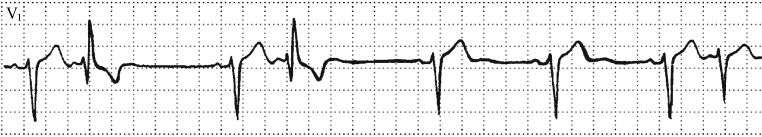
\includegraphics[width=3.21875in,height=2.30208in]{./images/Image00039.jpg}
\end{table}

\hypertarget{text00020.htmlux5cux23CHP1-7-2-1-1-4}{}
(4) 头痛的性质:

对头痛性质的了解十分重要。搏动性跳痛常为血管性头痛;发作性电击样剧痛为三叉神经痛的特征;咽后部发作性疼痛,可因吞咽动作诱发或加重者应考虑舌咽神经痛;紧箍样头痛多为肌紧张性头痛;眼、耳、鼻疾病所伴发者,大多数是胀痛或钝痛;神经症则是隐隐作痛,时轻时重。

\hypertarget{text00020.htmlux5cux23CHP1-7-2-1-1-5}{}
(5) 头痛的程度:

头痛的程度常不能反映病情的严重度,有时颅内占位性病变头痛并不严重而慢性焦虑症的头痛却表现剧烈难忍。一般而言,剧烈头痛常见于神经痛、偏头痛、蛛网膜下腔出血、脑膜炎等;中等度头痛,主要见于颅内占位性病变、慢性炎症等;轻度头痛,可见于神经症及某些邻近器官(耳、眼、鼻)病变。

\hypertarget{text00020.htmlux5cux23CHP1-7-2-1-1-6}{}
(6) 头痛发生的速度及影响因素:

急性突发性头痛,除多为血管性头痛外,尚有急性脑卒中(蛛网膜下腔出血、脑出血等)、急性感染性疾患。缓慢发生的头痛且进行性加重,并有颅内压增高表现者可能为颅内占位性病变,而无颅内压增高者可见于紧张性头痛。咳嗽、用力或头部转动,常使颅内压增高而头痛加剧;直立位可使肌紧张性头痛或腰穿后反应等加重,而丛集性头痛则减轻;压迫颞、额部动脉或颈总动脉可使血管性头痛减轻。根据头痛的发病方式和经过,对头痛进行鉴别诊断,见表\ref{tab7-2}。

\hypertarget{text00020.htmlux5cux23CHP1-7-2-1-1-7}{}
(7) 头痛的伴随症状:

头痛时常伴恶心、呕吐、面色苍白、出汗、心悸等自主神经症状,主要见于偏头痛;头痛严重并有进行性加剧的恶心、呕吐,常为颅内高压的征兆;体位变化时出现头痛加重或意识障碍,见于脑室内肿瘤、后颅凹或高颈段病变;伴有视力障碍及其他眼部征象(复视),呈短暂性发作者,多为偏头痛、椎-基底动脉供血不足;眼底视乳头水肿或出血,常为颅内压增高症或高血压性脑病。头痛伴精神症状(如淡漠或欣快)者应考虑额叶肿瘤的可能。由颅内损害引起的头痛常伴有神经功能缺失症状。

\hypertarget{text00020.htmlux5cux23CHP1-7-2-1-1-8}{}
(8) 其他病史:

尚需注意全身其他系统器官受损的病史,以及家族史、用药史、外伤史、手术史、月经及烟酒嗜好等。

\begin{table}[htbp]
\centering
\caption{头痛的发病方式和经过}
\label{tab7-2}
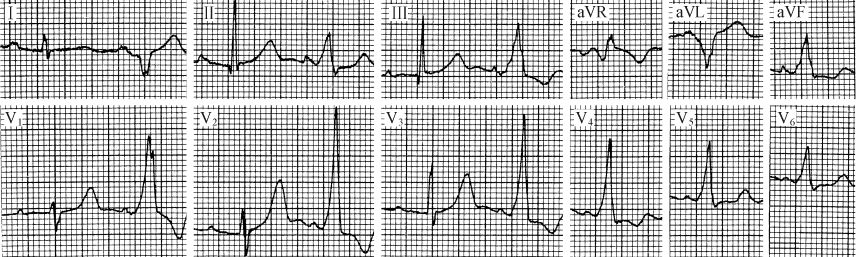
\includegraphics[width=3.22917in,height=4.33333in]{./images/Image00040.jpg}
\end{table}

\subparagraph{体检}

全面详尽的体格检查尤其是神经系统和头颅五官的检查,有助于发现头痛的病变所在。

\hypertarget{text00020.htmlux5cux23CHP1-7-2-1-2-1}{}
(1) 内科检查:

许多内脏器官或系统的疾患可发生头痛,应按系统详细检查,大多可查出头痛的原因。如高血压、全身感染性疾病的发热或中暑、缺氧(如一氧化碳中毒),慢性肺部疾患的高碳酸血症,严重贫血或红细胞增多症,均可由于脑血流增加而致头痛;而毒素作用、酗酒,则可因血管扩张而致头痛。尚有代谢内分泌疾病的检查(甲亢、低血糖、嗜铬细胞瘤等)。

\hypertarget{text00020.htmlux5cux23CHP1-7-2-1-2-2}{}
(2) 五官检查:

头部邻近器官的疾病也是头痛常见的原因。如在眼部的视神经炎、儿童的屈光不正、青光眼、眼部表浅炎症(结膜炎、角膜炎、睑板腺炎、泪囊炎等)及眶部组织的炎症;在耳鼻咽喉方面有鼻炎、鼻窦炎、咽炎、中耳炎、鼻窦或鼻咽部肿瘤,另外颞颌关节病及严重的牙病也可引起头痛。

\hypertarget{text00020.htmlux5cux23CHP1-7-2-1-2-3}{}
(3) 神经系统检查:

全面的神经系统检查是非常重要的。

\hypertarget{text00020.htmlux5cux23CHP1-7-2-1-2-4}{}
(4) 精神检查:

有不少精神科疾病可伴有头痛,神经症是最常见的,而抑郁症的精神症状可被躯体症状所掩盖,尤其是隐匿性抑郁,常呈一些不典型的疼痛。

\subparagraph{辅助检查}

应根据患者的具体情况和客观条件来选择性地应用。如做头颅X线检查、脑电图、CT扫描或MRI、腰穿脑脊液检查等,以及内科与五官科方面的检查。

头痛的临床检查方法见表\ref{tab7-3}。

\hypertarget{text00020.htmlux5cux23CHP1-7-2-2}{}
(二) 局限性病变抑或全身性病变

\subparagraph{局限性病变}

包括颈部以上的局部病变引起的头痛,又可分为两大组:

\begin{table}[htbp]
\centering
\caption{头痛的临床检查方法}
\label{tab7-3}
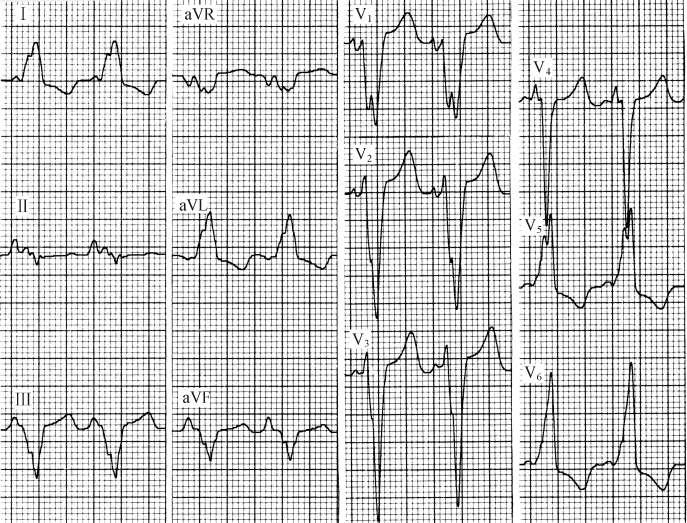
\includegraphics[width=3.25in,height=4.30208in]{./images/Image00041.jpg}
\end{table}

\hypertarget{text00020.htmlux5cux23CHP1-7-2-2-1-1}{}
(1) 颅内疾病:

此组疾病所致的头痛大都较严重,起病急,发展迅速。多数伴有恶心和(或)呕吐;部分尚有意识障碍或脑部和脑神经损害的表现,如抽搐、肢体瘫痪和瞳孔改变等。

\hypertarget{text00020.htmlux5cux23CHP1-7-2-2-1-2}{}
(2) 头颈部疾病:

此组疾病引起的头痛可轻可重,但很少逐渐加重。头痛的部位常与病灶一致或位于病灶附近,刺激病变部位可使疼痛加剧(如三叉神经痛等);但血管性头痛,压迫颞动脉则可使头痛减轻。头颈部疾病所致头痛的原发病灶明显,诊断不难。

\subparagraph{全身性病变}

\hypertarget{text00020.htmlux5cux23CHP1-7-2-2-2-1}{}
(1) 全身性器质性病变:

引起急性头痛主要包括两大类疾病:一类是急性中毒。金属及化学物质如铅、锰、苯、酒精、一氧化碳等中毒时均可引起头痛。常为头部弥漫性跳痛,转动头部,头痛部位和性质无改变为此类头痛的重要特点。另一类是全身感染。多为急性传染病,头痛多在疾病的初期发生,也可出现在传染病的极期;无脑膜刺激征及神经系统定位征,脑脊液压力有时可增高,但生化及外观检查无异常。

\hypertarget{text00020.htmlux5cux23CHP1-7-2-2-2-2}{}
(2) 功能性病变:

多见于神经症患者,除头痛外,常伴有神经症的其他症状,如失眠、记忆力减退、注意力不集中、头昏、烦躁等,常因精神刺激而加重。患者一般情况好,临床检查无器质性病变存在。部分患者的头痛是由于服药后所引起(医源性头痛),主要是血管扩张剂等。应注意,功能性头痛必须在排除可能的器质性病变后才能确立。

\subsection{处理原则}

头痛的防治原则包括病因治疗、对症治疗和预防性治疗。对于病因明确的病例应尽早去除病因,如颅内感染应抗感染治疗,颅内高压者宜脱水降颅压等。任何头痛在急性发作时均应尽可能寻找潜在的病因进行治疗;对于病因不能立即纠正的继发性头痛及各种原发性头痛急性发作,可给予止痛等对症治疗以终止或减轻头痛症状。对慢性头痛呈反复发作者应给予适当的预防性治疗,以防头痛频繁发作。

\subsection{常见头痛的诊断与处理}

\hypertarget{text00020.htmlux5cux23CHP1-7-4-1}{}
(一) 偏头痛

偏头痛(migraine)是一种常见的慢性神经血管性疾患,是临床常见的原发性头痛,其特征是发作性、多为偏侧、中重度、搏动样头痛,一般持续4~72小时,可伴有恶心、呕吐,光、声刺激或日常活动均可加重头痛,安静环境、休息可缓解头痛。多起病于儿童和青春期,中青年期达发病高峰,女性多见,约50\%患者有家族史。精神紧张、过度劳累、气候骤变、强光刺激、烈日照射、低血糖、应用扩血管药物或利血平、食用高酪胺食物(如巧克力、乳酪、柑橘)及酒精类饮料,均可诱发偏头痛发作。

\subparagraph{临床表现特点}

偏头痛有多种类型,但以以下两型常见:

\hypertarget{text00020.htmlux5cux23CHP1-7-4-1-1-1}{}
(1) 无先兆偏头痛(普通型偏头痛):

是最常见的偏头痛类型,约占80\%。临床表现为反复发作的一侧或双侧额颞部搏动性疼痛,常伴有恶心、呕吐、畏光、畏声、出汗、全身不适与头皮触痛等症状。通常在发作开始时仅为轻~中度的钝痛或不适感,数分钟至数小时后达到严重的搏动性痛或跳痛。有时疼痛放射至上颈部及肩部。部分女性患者发作常与月经有关,通常为经期前2天到经期的第3天之间发病,若90\%的发作与月经周期密切相关称月经期偏头痛。出现上述发作至少5次,除外颅内外各种器质性疾病后方可作出诊断。

\hypertarget{text00020.htmlux5cux23CHP1-7-4-1-1-2}{}
(2) 有先兆偏头痛(典型偏头痛):

约占偏头痛患者的10\%。一般在青春期发病,多有家族史,头痛发作前数小时至数日可有倦怠、注意力不集中和打哈欠等前驱症状。在头痛之前或头痛发生时,常以可逆的局灶性神经系统症状为先兆,表现为视觉、感觉、言语和运动的缺损或刺激症状。最常见为视觉先兆,常为双眼同向症状(homonymous
visual
symptoms),如视物模糊、暗点、闪光、亮点亮线或视物变形;其次为感觉先兆,感觉症状多呈面-手区域分布;言语和运动先兆少见。先兆症状一般在5~20分钟内逐渐形成,持续不超过60分钟;不同先兆可以接连出现。头痛在先兆同时或先兆后60分钟内发生,表现为一侧或双侧额颞部或眶后搏动性头痛,常伴有恶心、呕吐、畏光或畏声、苍白或出汗、多尿、易激怒、气味恐怖或疲劳感等,可见头面部水肿、颞动脉突出等。活动能使头痛加重,睡眠后可缓解头痛。头痛可持续4~72小时,消退后常有疲劳、倦怠、烦躁、无力和食欲差等,1~2日后常可好转。

有上述典型偏头痛症状,虽经治疗头痛时间持续在72小时以上(其间可能有短于4小时的缓解期)的称为偏头痛持续状态(status
migrainous)。

大多数偏头痛患者的预后良好,随年龄的增长症状可逐渐缓解,部分患者可在60~70岁时偏头痛不再发作。

\subparagraph{治疗要点}

偏头痛的治疗目的为减轻或终止头痛发作,缓解伴发症状,预防头痛复发。

\hypertarget{text00020.htmlux5cux23CHP1-7-4-1-2-1}{}
(1) 发作期的治疗:

治疗药物包括非特异性止痛药如非甾体类抗炎药(NSAIDs)和阿片类药物,特异性药物如麦角类制剂(麦角胺1~2mg/次,日最大剂量6mg;双氢麦角胺肌肉注射1~2mg/次,日最大剂量4mg,或口服1~3mg/次,日最大剂量9mg)和曲普坦类药物,后者包括舒马曲普坦(皮下注射:6mg/次,日最大剂量12mg;口服25~100mg/次,日最大剂量300mg)、那拉曲普坦(口服2.5mg/次,日最大剂量5mg)、利扎曲普坦(口服5~10mg/次,日最大剂量30mg)、佐米曲普坦(口服2.5~5mg/次,日最大剂量10mg)和阿莫曲普坦(口服6.25~12.5mg/次,日最大剂量25mg)等。通常应在症状起始时立即服药。药物选择应根据头痛程度、伴随症状、既往用药情况等综合考虑,可采用阶梯法、分层选药,进行个体化治疗。①轻~中度头痛:单用NSAIDs如对乙酰氨基酚(口服0.3~0.6g/次,日最大剂量不超过2.0g)、萘普生(口服0.2~0.3g/次,每日2~3次)、布洛芬(口服0.2~0.4g/次,每日3~4次)等可有效,如无效再用偏头痛特异性治疗药物。阿片类制剂如哌替啶等,因有成瘾性,不推荐常规用于偏头痛的治疗,但对于有麦角类制剂或曲普坦类应用禁忌的病例,如合并心脏病、周围血管病或妊娠期偏头痛,则可给予哌替啶治疗以终止偏头痛急性发作。②中~重度头痛:可直接选用偏头痛特异性治疗药物以尽快改善症状,部分患者虽有严重头痛但以往发作对NSAIDs反应良好者,仍可选用NSAIDs。麦角类和曲普坦类药物不良反应包括恶心、呕吐、心悸、烦躁、焦虑、周围血管收缩,大量长期应用可引起高血压和肢体缺血性坏死。严重高血压、心脏病和孕妇患者均为禁忌。此外,应用过频,则会引起药物过量使用性头痛(medication-overuse
headache),因此,麦角类和曲普坦类药物每周用药不超过2~3天。③伴随症状:恶心呕吐可肌肉注射甲氧氯普胺10mg,严重呕吐者可用小剂量奋乃静、氯丙嗪。烦躁者可用地西泮10~20mg肌肉注射以促使患者镇静和入睡。

\hypertarget{text00020.htmlux5cux23CHP1-7-4-1-2-2}{}
(2) 预防性治疗:

适用于:①频繁发作,尤其是每周发作1次以上严重影响日常生活和工作的患者;②急性期治疗无效,或因副作用和禁忌证无法进行急性期治疗者;③可能导致永久性神经功能缺损的特殊变异型偏头痛,如偏瘫性偏头痛、基底型偏头痛或偏头痛性梗死等。常用药物有:①β受体阻滞剂:普萘洛尔(10~60mg/次,每天2次),美托洛尔(100~200mg/次,每天1次);②钙通道阻滞剂:氟桂利嗪(5~10mg,每日1次,睡前服用),维拉帕米(160~320mg/d);③抗癫痫药:丙戊酸钠(0.4~0.6g/次,每天2次),托吡酯(25~200mg/d),加巴喷丁(0.9~1.8g/d);④抗抑郁药:阿米替林(25~75mg睡前服用),丙米嗪和氟西汀等;⑤5-HT受体拮抗剂:苯噻啶(0.5~3mg/d)等。其中,普萘洛尔、阿米替林和丙戊酸钠三种在结构上无关的药物,是预防性治疗的支柱,一种药物无效可选用另一种药物。

\hypertarget{text00020.htmlux5cux23CHP1-7-4-2}{}
(二) 丛集性头痛

丛集性头痛(cluster
headache)是一种原发性神经血管性头痛。以男性多见,约为女性的3~4倍。头痛突然发生,无先兆症状,几乎于每日同一时间,常在晚上发作,使患者从睡眠中痛醒。头痛位于一侧眶周、眶上、眼球后和(或)颞部,呈尖锐、爆炸样、非搏动性剧痛。头痛达高峰时,患者常以手击头部、甚至以头撞墙,在室内外来回走动、十分烦躁、痛苦与不安。头痛持续15分钟~3小时不等。发作频度不一,从一日8次至隔日1次。疼痛时常伴有同侧颜面部自主神经功能症状,表现为结膜充血、流泪、流涕等副交感神经亢进症状,或瞳孔缩小和眼睑下垂等Horner征,较少伴有恶心、呕吐。头痛发作可连续数周至数月(常为2周~3个月),在此期间患者头痛呈一次接一次地成串发作,故名丛集性头痛。丛集发作期常在每年的春季和(或)秋季;丛集发作期后可有数月或数年的间歇期。在丛集期,饮酒或血管扩张药可诱发头痛发作,而在间歇期,两者均不会引起头痛发作。

根据中青年男性出现发作性单侧眶周、眶上和(或)颞部严重或极度严重的疼痛,可伴有同侧结膜充血、流泪、流涕、眼睑水肿、前额和面部出汗、瞳孔缩小、眼睑下垂等自主神经症状,发作时坐立不安、易激惹,并具有反复密集发作的特点,神经影像学排除引起头痛的颅内器质性疾患,可作出丛集性头痛的诊断。

本病急性期治疗方法有:①吸氧疗法:为头痛发作时首选的治疗措施。在发作剧烈时吸入纯氧(100\%氧气8~10L/min,10~20分钟)约使70\%患者终止发作。②利多卡因:用4\%~10\%利多卡因1ml经患侧鼻孔滴入,可使1/3的患者头痛缓解,机制是麻醉蝶腭神经节。③舒马曲普坦6mg皮下注射,或双氢麦角胺1~2mg肌肉注射等,可迅速缓解头痛。

本病预防性治疗药物包括维拉帕米、锂制剂和糖皮质激素等。维拉帕米240~320mg/d可有效预防本病发作,可在用药2~3周内发挥最大疗效。锂制剂适用于其他药物无效或有禁忌证者。糖皮质激素如泼尼松40~60mg/d,常可预防头痛的发作,第2周逐渐减量停药。其他药物有托吡酯、丙戊酸钠、苯噻啶、吲哚美辛等。

\hypertarget{text00020.htmlux5cux23CHP1-7-4-3}{}
(三) 紧张型头痛

紧张型头痛(tension-type headache)又称肌收缩性头痛(muscle contraction
headache),是双侧枕部或全头部紧缩性或压迫性头痛,约占头痛患者的40\%,是临床最常见的慢性头痛。主要由精神紧张及颅周肌肉张力增高引起。长期焦虑、紧张、抑郁或睡眠障碍,高强度的工作缺乏适当的放松及休息,以及某些单调工种使头、颈或肩胛带长期处于不良的姿势等均可为发病因素。头痛部位不定,可为双侧、单侧、全头部、颈项部、双侧枕部、双侧颞部等不同部位。通常呈持续性钝痛,像一条带子紧束头部或呈头周紧箍感、压迫感或沉重感。许多患者可伴有头昏、失眠、焦虑或抑郁等症状。有的患者也可出现恶心、畏光或畏声等症状。体检可发现疼痛部位肌肉触痛或压痛点,有时牵拉头发也有疼痛,颈肩部肌肉有僵硬感,捏压时肌肉感觉舒适。

根据患者的临床表现,排除颅颈部疾病如颈椎病、占位性病变和炎症性疾病等,通常可以确诊。

本病的许多治疗药物与偏头痛用药相同。对于焦虑、紧张或抑郁的患者应在精神上给予诱导和安慰,使其消除顾虑。对局限性的肌肉疼痛,如颈项肌和肩胛肌等可作按摩、针灸、理疗、局部封闭等治疗。急性发作期用对乙酰氨基酚、阿司匹林、非甾体抗炎药、麦角胺或双氢麦角胺等亦有效。对于频发性和慢性紧张型头痛,应采用预防性治疗,可选用阿米替林、丙米嗪或选择性5-羟色胺重摄取抑制剂(如舍曲林或氟西汀),或肌肉松弛剂如盐酸乙哌立松、巴氯芬等。失眠者可给予苯二氮{}
类如地西泮10~20mg/d口服。

\hypertarget{text00020.htmlux5cux23CHP1-7-4-4}{}
(四) 颅内压变化引起的头痛

\subparagraph{颅内压增高所致的头痛}

脑瘤、硬膜下血肿、脑脓肿及其他占位性病变引起的头痛,在初期主要是因病变邻近疼痛敏感结构被牵拉、移位或因感觉神经直接受压所致。在后期是由于脑脊液循环通路被阻塞,导致颅内压增高,使远离病灶的对疼痛敏感结构被牵拉、扭曲和移位而引起头痛。初期的头痛常位于占位病变的同侧,在后期有颅内压增高时呈现为弥漫深在的持久性钝痛,晨起较重,在咳嗽、大便用力或打喷嚏时头痛加重。头痛程度一般不如偏头痛或颅内出血时那样严重,多数不影响睡眠。随着占位病变增大及颅内压增高,患者出现呕吐及视乳头水肿,最后因继发性视神经萎缩使视力减退或双目失明。治疗上除应用脱水剂降低颅内压外,根本措施是手术切除占位性病变。

良性颅内压增高征指有头痛和视乳头水肿等颅内压增高表现而无局灶性神经系统体征,抽搐、精神障碍,其脑室系统和脑脊液成分基本正常,颅内无占位性病变,预后较为良好的一种临床综合征。此症患者大都诉述有全面性的头痛,而并无脑部结构的移位,头痛可能是由于伴发的脑水肿牵引脑膜与脑血管的神经末梢所致。

\subparagraph{低颅压性头痛}

低颅压性头痛(intracranial hypotension
headache)是脑脊液(CSF)压力降低(< 60mmH\textsubscript{2}
O)导致的头痛,多为体位性。患者常在直立后15分钟内出现头痛或头痛明显加剧,卧位后头痛缓解或消失。

低颅压性头痛包括自发性(特发性)和继发性两种。自发性病因不明,既往多认为可能与血管舒缩障碍引起CSF分泌减少或吸收增加有关;目前已证实多数自发性低颅压与自发性脑脊液漏有关。而导致自发性脑脊液漏可能与微小创伤和硬膜结构薄弱有关。部分病例有剧烈咳嗽、推举重物、剧烈体育活动等引起微小创伤的病史;部分病例可合并有结缔组织异常的其他疾病,如马方综合征(Marfan
syndrome)、常染色体显性遗传多囊肾、自发性视网膜脱离等。继发性可由多种原因引起,其中以硬膜或腰椎穿刺后低颅压性头痛最为多见,头颈部外伤及手术、脑室分流术、脊柱创伤或手术使CSF漏出增多,脱水、糖尿病酮症酸中毒、尿毒症、全身严重感染、脑膜脑炎、过度换气和低血压等使CSF生成减少。由于CSF量减少,压力降低,脑组织移位下沉等使颅内疼痛敏感组织被牵拉引起头痛。

本病可见于各种年龄,特发性多见于体弱女性,继发性无明显性别差异。头痛以双侧枕部或额部多见,也可为颞部或全头痛,但很少为单侧头痛,呈轻~中度钝痛或搏动性疼痛,缓慢加重,常伴恶心、呕吐、眩晕、耳鸣、颈僵和视物模糊等。头痛与体位有明显关系,立位时出现或加重,卧位时减轻或消失。脑组织下坠压迫脑神经也可引起视物模糊或视野缺损(视神经或视交叉受压)、面部麻木或疼痛(三叉神经受压)、面瘫或面肌痉挛(面神经受压)。

病因明确者应针对病因治疗,如控制感染、纠正脱水和糖尿病酮症酸中毒等。对手术或创伤后存在脑脊液瘘者可行瘘口修补术等。对症治疗包括头低位卧床休息,补液(2000~3000ml/d),穿紧身裤和束腹带,给予适量镇痛剂等。鞘内注射无菌生理盐水可使腰穿后头痛缓解。咖啡因可阻断腺苷受体,使颅内血管收缩,增加CSF压力和缓解头痛,可用苯甲酸钠咖啡因0.5g皮下或肌肉注射,或加入500~1000ml林格液中静脉滴注。硬膜外血贴疗法(epidural
blood
patching)是用自体血15~20ml缓慢注入腰或胸段硬膜外间隙,血液从注射点上下扩展数个椎间隙,可压迫硬膜囊和阻塞脑脊液漏出口,迅速缓解头痛,适用于腰穿后头痛和自发性低颅压性头痛,有效率97\%。腰穿时应选用口径细的穿刺针,术后去枕平卧至少6小时有利于预防头痛。

\hypertarget{text00020.htmlux5cux23CHP1-7-4-5}{}
(五) 脑血管病所致头痛

脑血管病所致头痛是急性头痛患者首先要甄别的,包括蛛网膜下腔出血、脑出血、缺血性卒中等。

\subparagraph{蛛网膜下腔出血}

急性发作的头痛首先应考虑蛛网膜下腔出血的可能。典型症状为急性发作剧烈头痛,主诉为“刀劈样”、“爆炸样”头痛。70\%的头痛无定侧,可以为双额、顶、枕部或满头痛,30\%头痛偏向一侧,通常偏向动脉瘤所在侧。疼痛可放射至一侧或双侧眼部或颈部,可沿颈项向下放射,出现颈项强直,可持续数周至数月。可有意识丧失。也有一部分患者首发症状为精神错乱,惊厥发作,眩晕或脑神经(常为动眼神经瘫痪)障碍。腰穿脑脊液为均匀血性。患者如以往经常有阵发性头痛,此次头痛发作比较急剧,性质不同以往,也要考虑蛛网膜下腔出血。其处理参见第84章第4节“蛛网膜下腔出血”。

\subparagraph{脑出血}

头痛常为首发症状,但往往迅速出现意识障碍与肢体偏瘫,结合血压突然升高的背景,诊断不难。

\subparagraph{未破裂的脑动脉瘤与动静脉畸形}

一般在动脉瘤未破裂之前,头痛是不常见的。脑血管畸形头痛时常位于畸形同侧,如后交通动脉或颈内动脉瘤可以引起固定在同侧的眶、额部头痛。动脉瘤进一步扩张时可以出现眼肌瘫痪或对侧视野缺损,可以有局限性癫痫发作,对侧肢体偏瘫。DSA和(或)头颅MRI检查有助于诊断,治疗以手术为主。

\subparagraph{缺血性脑卒中}

少数脑栓塞病例中有头痛症状,而在脑血栓形成中则头痛不常见。脑供血不足可致头痛,伴同感觉与运动障碍。头痛往往是搏动性的,可能是继发于颅外动脉的扩张。在椎-基底动脉或颈内动脉狭窄或闭塞的病例中,约1/3~1/2的患者有头痛,大都局限于枕部和颈部,或两额部;颈内动脉供血不足的头痛可以是同侧的或对侧的。

\subparagraph{颞动脉炎}

颞动脉炎(temporal
arteritis)多见于中、老年人,头痛常位于头皮表浅部位以及颞部与眼眶周围部,也可较广泛地弥漫及额部与枕部,为一种强烈的搏动性和持续性疼痛,并且伴有在其他血管性头痛中所没有的烧灼感。平卧位或头低位头痛加剧,仰头或压迫颈总动脉时头痛减轻,咀嚼时头痛加重。咀嚼时出现头痛常为本病的首发症状。压迫眼球或眼球转动即出现眼窝部疼痛。头痛同时伴有面部肿胀、皮肤红肿、颞动脉明显扩张隆起呈蛇行状,搏动消失,触之有发硬肥厚感,压痛明显。部分病例视网膜动脉或脑动脉也可受累,可发生缺血性视神经炎而出现视力障碍。颞动脉炎多有发热、出汗、疲乏等全身症状,周围血象有白细胞增高,血沉增快。

本病如不加特殊治疗,通常在3~24个月内病情渐趋稳定或自愈,少数可持续几年。治疗主要用肾上腺皮质激素且疗效好,在激素开始治疗后数小时内体温即下降为正常,1~2天内局部疼痛和全身症状消失,食欲正常。头痛消失后激素可渐减量并维持用药数月,如停药后复发可重复再用。

\hypertarget{text00020.htmlux5cux23CHP1-7-4-6}{}
(六) 高血压性头痛

是一种非偏头痛型血管性头痛
。高血压病时约80\%出现不同程度头痛,且青壮年的高血压病头痛发生率高,其机制与动脉壁痛觉感受器受刺激有关。表现为头部沉重或间歇性钝痛、压迫感或搏动痛,或呈持续性全头或偏侧头痛,部位不固定,多在清晨或午前出现,在低头或屏气用力后头痛可加剧。恶性高血压伴高血压脑病或因嗜铬细胞瘤血压突然升高时均可出现剧烈的持续性头痛,常伴有恶心、呕吐、视力减退,视网膜出血或视乳头水肿。

高血压性头痛的治疗在于及时适度的降低血压。对伴有脑水肿者应及时应用脱水剂。

\hypertarget{text00020.htmlux5cux23CHP1-7-4-7}{}
(七) 颅脑外伤性头痛

急性和慢性头部外伤均可伴有头痛,常见的外伤后头痛有下列几种类型:①头皮裂伤或脑挫裂伤后瘢痕形成,刺激颅内外痛觉敏感结构而引起头痛。疼痛部位较局限,常伴局部皮肤痛觉过敏。②外伤后自主神经功能异常性头痛(dysautonomic
headache)是因颈前部受伤累及颈交感神经链,导致支配头颅的交感神经失去抑制而引起头痛。患者叙述一侧额颞区的发作性头痛,伴同侧瞳孔改变(先扩大后缩小),眼睑下垂及面部多汗。服用普萘洛尔(20mg,每天3次)对头痛有效。③外伤后因颈肌持续收缩而出现头痛,和紧张型头痛相似常有精神因素参与。④外伤后神经不稳定性头痛。常见于脑震荡后遗症,除头痛外尚有头晕、耳鸣、失眠、注意力不集中,记忆力衰退,精神萎靡不振或情绪易激动等症状。神经系统无器质性损害证据。

\hypertarget{text00020.htmlux5cux23CHP1-7-4-8}{}
(八) 五官疾病的头痛

眼源性头痛是指青光眼、虹膜炎、眼眶肿瘤、球后视神经炎、高度远视、眼外肌不平衡及用眼时间过长等原因引起球后或额颞区疼痛。急性乳突炎能引起耳后疼痛。病毒性膝状神经节带状疱疹所产生的疼痛常位于外耳道内或耳后,疼痛数日后出现带状疱疹及面瘫。鼻腔或鼻窦发炎时因黏膜充血水肿而引起鼻塞、流涕及牵涉性头痛。急性鼻窦炎时常引起眼球周围或额颞区头痛。因鼻窦内的脓性分泌物经过一夜睡眠后积聚增多,故患者清晨起床后头痛特别严重,待脓液排出后头痛明显减轻。X线检查有助于本病诊断。个别患者因鼻窦窦口被炎性分泌物或过敏性水肿阻塞,鼻窦内压力降低而形成“真空性头痛”(vacuum
headache)。牙病所致的头痛,多先有病牙部位疼痛,随后放射至同侧颞部,呈灼痛或跳痛,牙科检查可确诊。鼻腔肿瘤、颞下颌关节功能障碍(Costen综合征)及鼻咽癌均可引起头部牵涉痛。

\hypertarget{text00020.htmlux5cux23CHP1-7-4-9}{}
(九) 精神性头痛

神经症
、抑郁症等,经常出现头痛。其部位多不固定,多变,性质多样,呈钝痛、胀痛,易受外界或情绪影响,历时数周甚至数年。常伴睡眠及记忆、理解等精神方面的症状。

\hypertarget{text00020.htmlux5cux23CHP1-7-4-10}{}
(十) 神经痛

\subparagraph{三叉神经痛(trigeminal neuralgia)}

是指三叉神经分布区内短暂的反复发作性剧痛。成年及老年人多见,40岁以上患者占70\%~80\%,女性多于男性。三叉神经痛可分为症状性和原发性,前者的病因为炎症(如疱疹病毒感染)、肿瘤(如半月神经节肿瘤)、动脉瘤及外伤等,后者系指病因未明者(可能因三叉神经脱髓鞘产生异位冲动或伪突触传递所致)。典型的原发性三叉神经痛通常有如下特点:①疼痛常局限于一侧,并以累及一支多见,少数患者可同时有二支或三支受累,且以上颌支(第2支)或下颌支(第3支)最常受累。②疼痛发作时表现为以面颊上下颌及舌部明显的剧烈电击样、刀割样、烧灼样或撕裂样疼痛,来去骤然,突发突止。疼痛由颌面或牙槽病灶开始,并沿该神经的支配区域放射,每次发作仅数秒钟至1~2分钟,间歇期正常,1天数次至1分钟多次。发作呈周期性,持续数周,可自行缓解数月或更长。随病程进展,缓解期日益缩短。③发作时可伴有同侧面部肌肉的反射性抽搐(故又称“痛性抽搐”),或有同侧面部潮红、流泪及流涎。④患者面部某个区域可能特别敏感,稍加触碰即引起疼痛发作,如上下唇、鼻翼外侧、舌侧缘、颊部等,该区域称之为“扳机点(触发点)”。发作期间面部的机械刺激,如说话、进食、洗脸、剃须、刷牙、打哈欠,甚至微风拂面皆可诱致疼痛发作,患者因而不敢大声说话、洗脸或进食,有的连口水也不敢咽下,严重影响患者生活,甚至全身营养状况不良,精神抑郁,有的产生消极情绪。

治疗主要有药物、封闭和手术治疗。药物治疗以卡马西平为首选,起始剂量0.1g口服,每天2~3次,最大剂量1.0g/d,有效维持量0.6~0.8g/d。如卡马西平无效可改用苯妥英钠0.1g口服,每天3次,如无效可每日增加0.05g,数日后加至0.6g/d。卡马西平或苯妥英钠单药治疗无效者两药合用可能有效。上述两药无效时可试用氯硝西泮(clonazepam)6~8mg/d口服。大剂量维生素B\textsubscript{12}
可缓解疼痛,剂量为1000~2000μg肌肉注射,每周2~3次,连用4~8周为一疗程。药物治疗无效者可试用无水乙醇或甘油封闭三叉神经分支或半月神经节,破坏感觉神经细胞,可获止痛效果,不良反应为注射区面部感觉缺失。经皮半月神经节射频电凝疗法也有较好疗效。三叉神经感觉根部分切除术,因止痛效果确切,仍是首选的手术治疗方法。而三叉神经显微血管减压术,止痛同时不产生感觉及运动障碍,是目前广泛应用的最安全有效的方法。

\subparagraph{舌咽神经痛}

舌咽神经分布区的反复阵发性剧痛,不伴脑神经功能破坏表现的称舌咽神经痛(glossopharyngeal
neuralgia)。远比三叉神经痛少见。多数于中年起病,表现为口咽、喉或耳内的短暂发作性剧痛。每次持续数秒至1分钟,可因吞咽、咀嚼、讲话、咳嗽等触发。检查咽喉、舌根和扁桃体窝可有疼痛触发点。疼痛发作时可伴发咳嗽。个别患者发生昏厥,可能由于颈动脉窦神经过敏引起心脏停搏而造成。病程中可有自发缓解。神经系统检查无异常发现。将4\%可卡因或1\%丁卡因涂于患侧的口咽部,常可使疼痛缓解数小时。病因不明,有的可能是由于舌咽神经的脱髓鞘性病变引起,有的可能是由于局部的颅底血管压迫于舌咽神经所致。若疼痛持续,则本病需与鼻咽癌侵及颅底、耳咽管肿瘤、扁桃体肿瘤相鉴别。治疗与三叉神经痛相似。

\subparagraph{枕神经痛}

枕神经痛(occipital
neuralgia)是枕大、枕小和耳大神经分布区疼痛的统称,三对神经来自C\textsubscript{2~3}
神经,分布于枕部。可因上段颈椎病、脊柱结核、骨关节炎、脊髓肿瘤、硬脊膜炎和转移瘤等所致,多为继发性神经损害;也可由上呼吸道感染或扁桃体炎引起,或病因不明。枕大神经分布于后枕部相当于两侧外耳道经头顶连线以后的部分;枕小神经主要分布于耳廓上部和枕外侧皮肤;耳大神经主要分布于耳廓下部前后面、腮腺表面和下颌角部皮肤。疼痛位于一侧枕部与颈部,呈阵发性刺痛或电击样痛,或持续性钝痛;患侧枕部头皮可有皮肤感觉过敏及局限性压痛点,可向头顶(枕大神经)、乳突部(枕小神经)或外耳(耳大神经)放射。枕大神经痛压痛点位于乳突与枕后粗隆间连线的中点;枕小神经痛的压痛点多位于该连线的外1/3处。部分患者在间歇期仍有钝痛。疼痛可为自发或因旋转尤其向对侧旋转而诱发,其他头颈部运动或咳嗽、喷嚏可使疼痛加重或诱发疼痛,故患者常不敢过分活动头部,或使头略向后仰并向患侧倾斜以缓解疼痛。除病因治疗外,可用止痛剂(卡马西平、苯妥英钠等)、神经营养剂(维生素B\textsubscript{1}
、B\textsubscript{12} 等)、局部封闭、理疗等对症治疗。


\hypertarget{text00021.htmlux5cux23CHP1-7-5}{}
参 考 文 献

1. 贾建平.神经病学.第6版,北京:人民卫生出版社,2008:158.

2. 头痛分类和诊断专家共识组
.头痛分类和诊断专家共识.中华神经科杂志,2007,40:439.

3. Schievink WI. Spontaneous spinal cerebrospinal fluid leaks and
intracranial hypotension. JAMA,2006,295:2286.

\protect\hypertarget{text00022.html}{}{}

\chapter{胸 痛}

胸痛是急诊室常见的患者就诊原因之一,临床上的胸痛不应仅是指解剖学胸部范围内的疼痛感受,而应包括任何原因所导致的解剖学胸部范围内的任何不适,同时也包括由于胸部疾患可能表现为其他部位的疼痛。由此可见导致胸痛的病因复杂,病情的严重程度相差很大。多数为良性经过的普通疾病,但其中有一部分则可能导致严重后果甚至危及生命。对于高危患者,症状发作后启动治疗越早,疗效越好,获益越多,任何延误都可能导致严重不良事件的发生,因此,急性胸痛患者的早期鉴别和危险分层对于识别高危患者并给予及时正确的处置具有重要意义。在临床急诊工作中,应首先确定就诊的急性胸痛患者是否患有急性心肌梗死、主动脉夹层、肺栓塞、气胸等,因为这些疾病若处理不及时,常危及生命。

\subsection{病因与发病机制}

\subsubsection{病因}

胸痛的主要病因大体上包括胸内结构病变、胸壁组织疾病、膈下脏器病变和功能性疾病等几个方面:

\subparagraph{胸内结构病变}

\hypertarget{text00022.htmlux5cux23CHP1-8-1-1-1-1}{}
(1) 心源性胸痛:

心绞痛、急性心肌梗死、急性心包炎、主动脉夹层等。

\hypertarget{text00022.htmlux5cux23CHP1-8-1-1-1-2}{}
(2) 非心源性胸痛:

①大血管病变:主动脉瘤、肺梗死;②呼吸系统疾病:胸膜炎、自发性气胸等;③纵隔和膈肌的疾病:纵隔炎、纵隔脓肿、纵隔肿瘤和膈疝等;④食管疾病:反流性食管炎、食管破裂、食管裂孔疝等。

\subparagraph{胸壁组织疾病}

带状疱疹、乳腺炎、皮下蜂窝组织炎、非化脓性肋软骨炎、肌炎、流行性肌炎、肋间神经炎、肋骨骨折等。

\subparagraph{膈下脏器病变}

膈下脓肿、肝脓肿、脾梗死和肝癌破裂等。

\subparagraph{功能性疾病}

心脏神经症。

\subsubsection{发病机制}

疼痛产生的机制:①各种化学或物理因素如缺氧、炎症、肌张力改变刺激肋间神经感觉纤维,脊髓后根传入纤维,支配气管、支气管及食管的迷走神经感觉纤维,膈神经的感觉纤维,支配心脏或主动脉感觉纤维等引起疼痛;②某一内脏与体表某一部位同受某些脊神经后根传入神经支配时,来自内脏的痛觉冲动传入大脑皮层区,除产生局部疼痛外,还可以出现相应体表的疼痛感觉------放射痛(又称牵涉痛)。

\subsection{诊断思路}

急性胸痛中包括了一组以胸痛为主要表现的疾病,其中危险性最高的分别是:急性心肌梗死、急性肺栓塞、主动脉夹层、张力性气胸及心包填塞。这些患者可能随时会发生死亡。急诊医生的任务是在众多表现为急性胸痛的患者中识别出这些高危的疾病并给予及时、适当的处理。这些高危的患者是否能够在急诊被及时准确地识别出来主要依靠:①急诊医生一定要时刻保持对这些疾病的警惕性;②急诊医生一定要掌握这些疾病主要的临床特征;③急诊科要有鉴别这些疾病的合理流程;④急诊科要能够提供必要的检查手段。

\subsubsection{临床特征}

首先在急诊处理急性胸痛的患者时,要利用有限的时间仔细询问病史和进行体格检查,这样能够确定下一步思考的正确方向。在询问病史时,要注意胸痛的部位、性质、缓解的因素,胸痛诱发和加重的因素,胸痛是否放射,胸痛的伴随症状和既往病史等。这些特征中往往隐含着具有诊断和鉴别诊断意义的线索,因此这些特征是医生接诊急性胸痛患者时需要重点询问的内容,相当部分的胸痛患者单纯依靠详细的病史询问就可以基本诊断。

\subparagraph{发病年龄}

青壮年胸痛,应注意自发性气胸、心肌炎、心肌病、风湿性心瓣膜病,40岁以上患者应注意心绞痛、心肌梗死与肺癌。

\subparagraph{胸痛部位}

包括疼痛部位及其放射部位。心绞痛与心肌梗死的疼痛常位于胸骨后或心前区,且放射到左肩和左上臂内侧。夹层动脉瘤疼痛位于胸背部,向下放射至下腹、腰部与两侧腹股沟和下肢。食管疾患、膈疝、纵隔肿瘤的疼痛也位于胸骨后。胸膜炎所致的胸痛常在胸廓的下侧部或前部。带状疱疹是成簇水疱沿一侧肋间神经分布伴剧痛,疱疹不越过体表中线。胸壁疾病特点为疼痛部位局限,局部有压痛。炎症性疾病,尚伴有局部红、肿、热表现。肝胆疾病或膈下脓肿可引起右下胸痛。

\subparagraph{持续时间}

心绞痛发作时间短暂,持续数分钟,而心肌梗死疼痛持续时间很长且不易缓解。炎症、肿瘤、栓塞或梗死所致疼痛呈持续性。平滑肌痉挛或血管狭窄缺血所致疼痛为阵发性。

\subparagraph{疼痛性质}

胸痛的程度可表现为剧烈的疼痛到轻微的隐痛,疼痛性质也多种多样。如带状疱疹呈刀割样痛或灼痛,剧烈难忍;肌痛呈酸痛;骨痛呈酸痛或锥痛。心绞痛常呈压榨样痛并伴有压迫感或窒息感;主动脉夹层动脉瘤常有突然出现的剧烈的撕裂痛。膈疝呈灼痛或膨胀感。早期肺癌可仅有胸部的钝痛或隐痛。食管疾病多表现为持续性隐痛或烧灼痛。

\subparagraph{伴随症状}

气管、支气管疾病所致胸痛常伴有咳嗽、咳痰;食管疾病所致胸痛常伴有吞咽困难或咽下疼痛;肺梗死、原发性肺癌的胸痛常伴有小量咯血或痰中带血。

\subparagraph{影响疼痛因素}

包括发生诱因、加重与缓解因素。胸膜炎、自发性气胸、心包炎所致胸痛常在深吸气及咳嗽时加重,停止呼吸运动则疼痛减轻或消失。劳累、体力活动、精神紧张,可诱发心绞痛发作,休息、含服硝酸酯类药物可使心绞痛缓解,而对心肌梗死疼痛则无效。反流性食管炎的胸骨后灼痛,饱餐后出现,仰卧或俯卧位加重,服用抗酸剂和促动力药后可减轻或消失。

\subsubsection{必要的体格检查}

对于急性胸痛患者,一般不可能进行全面、系统的体格检查,要求5分钟内完全必要的体格检查。因为大多数情况下病情不允许医生有充分的时间这样做,因此重要的是要有针对性,有目的地根据患者的病史特征和临床思维分析进行一些重点体查。

首先要注意生命征,包括血压、脉搏、呼吸、体温。发现患者血压<
90/60mmHg,心率> 100次/分钟,应立即启动稳定生命征治疗。

怀疑主动脉夹层对比双侧桡动脉、股动脉和足背动脉搏动,有怀疑应测四肢血压。

观察胸部表面皮肤有无局限性红肿、瘀斑和出血点及疱疹等;胸腹式呼吸协调性、呼吸形式和快慢深浅;双侧胸部对称性。胸膜炎、胸腹部外伤、膈下脓肿、单纯疱疹等疾病常有上述异常变化。触诊检查局部肿块、液波感、压痛和胸廓的呼吸动度。

注意胸壁感染、气胸、血胸、肋骨骨折等征象。女性乳腺炎也有以胸痛主诉就诊,注意鉴别。

听诊需了解双侧呼吸音对比、胸膜和心包摩擦音、肺干湿性啰音、哮鸣音、异常音和杂音等,这对鉴别心脏和肺部疾病有帮助。

怀疑肺栓塞的患者要注意检查下肢有无肿胀,是否有下肢深静脉血栓形成的证据。

\subsubsection{必要的辅助检查}

对胸痛的诊断,除需仔细了解病史、查体外,一些常规的辅助检查,如心电图(ECG)、心肌损伤标志物及影像学检查也十分重要,这对筛查潜在的高危胸痛患者有参考价值。

\subparagraph{实验室检查}

血常规检查和凝血功能对判断有无感染和出凝血异常的存在必不可少。初始的ECG有助于确定中~高危的ACS患者,肌钙蛋白和心肌酶学是确诊是否存在心肌损害的重要手段,应用肌钙蛋白有助于确定是否需要早期血运重建,是ACS危险分层的重要工具;D-二聚体对急性肺栓塞的诊断有重要意义;动脉血气分析有助于了解肺功能情况。

\subparagraph{心肌损伤标记物在胸痛患者中的应用价值}

心肌损伤标志物的测定能检出或除外心肌坏死,最常应用的生化标志物有肌钙蛋白T(TnT)和肌钙蛋白I(Tn
I)、肌红蛋白和肌酸激酶MB同工酶(CK-MB)。在急性胸痛的早期约3~6小时,肌红蛋白检测对除外心肌梗死的可能性很有价值,在症状发作7小时后,肌钙蛋白与CK-MB有较高的阴性预测性,Tn
I或TnT对诊断AMI的特异性与敏感性均较高。心肌损伤标记物浓度与心肌损害范围呈正相关。约30\%的非ST段升高的ACS患者cTn
I或cTnT升高,可能为非Q波心肌梗死而属高危患者,即使CK-MB正常,死亡危险性也增加。肌钙蛋白水平越高,危险性越高。

\subparagraph{心电图}

ECG是胸痛患者应用广泛的检查方法。异常的心电图包括ST段升高、ST段下降和T波低平或倒置。入院时ECG有ST段升高的患者早期死亡率最高,ST段下降患者的死亡率中等,T波倒置最低。ST段升高是急性心肌梗死最敏感和最特异的ECG标志。新出现ST段升高的患者80\%~90\%为急性心肌梗死。约90\%的ECG有新出现的Q波为急性心肌梗死。ST段下降提示心肌缺血,但是其诊断进展性心肌梗死的可靠性差,仅约50\%的患者最终确诊为急性心肌梗死。对称性T波倒置的特异性较差,心肌缺血、心肌炎和肺栓塞在内的多种疾病都可以出现这种改变,约1/3的患者可能存在心肌梗死。有1/3左右的急性胸痛患者ECG正常,对这些患者动态观察心电图的变化很重要。在发病早期,很多急性心肌梗死最初的心电图无异常,随着时间的延长才表现为急性心肌梗死典型的ST段升高的ECG表现,若未对患者进行动态观察,常易忽略而漏诊。

目前建议在胸痛患者来诊10分钟内应进行ECG检查,10分钟内做出判定,ST段升高的患者一旦确定需立即进行再灌注治疗;ECG有缺血性表现的患者,按不稳定性心绞痛或非ST段升高的急性心肌梗死处理;ECG正常或有非特异性改变,应结合病史和生化标志物等综合判断。

\subparagraph{影像学检查}

X线胸部透视与摄片,对于鉴别肺部疾病、肋骨、胸骨骨折,心脏各房室大小有帮助;CT扫描是一项对临床有较大帮助的检查,可以发现X线不能显示的病变,帮助临床诊断肺栓塞、主动脉瘤、夹层动脉瘤。心血管造影,尤其血管数字减影(DSA),可清楚显示主动脉瘤、主动脉夹层、室壁瘤的部位、大小、形态等情况;冠状动脉造影,可明确心肌梗死的部位和严重程度,是诊断心肌梗死的“金标准”;超声心动图实时显示心脏结构和动态以及心包积液。B超对膈下和肝脓肿、胆道情况以及包裹性胸水定位有意义。

\subparagraph{放射性核素扫描}

对肺梗死、肺内占位病变、心肌梗死或局限性室壁瘤的诊断有帮助。

\subparagraph{彩色多普勒超声}

对急性心肌梗死和急性大动脉夹层动脉瘤诊断的意义较大。彩超和多普勒可用于大动脉夹层的检查,但其具有一定的局限性。彩超仅能看到升主动脉和腹部、髂部的血管。主要的征象是主动脉明显增宽,主动脉壁分离形成的真腔与假腔,有时还可见内膜的裂口。超声还可用于鉴别胆石症、脾梗死、胰腺炎等一些膈下疾病。急性心肌梗死时二维超声心动图可见梗死的部位室壁运动低下、运动消失或反常运动。超声对急性肺栓塞的诊断帮助不大。超声对自发性气胸的诊断没有帮助。

\subparagraph{胸痛患者辅助检查的顺序}

决定检查的顺序时要根据:危险性最大、最需要首先排除的疾病是什么?最能明确诊断的检查是什么?最方便、最及时的检查是什么?对于所有胸痛的患者,首先是要进行详细的体格检查,尤其是要注意生命体征,其次才是借助仪器的检查。有些疾病经过仔细的体格检查就能够发现特征性的表现,如剧烈胸痛者发现脉搏不对称及血管杂音强烈提示大动脉夹层等。切忌一切依赖仪器。对于一个急性胸痛的患者,辅助检查应该按照以下顺序进行为宜:

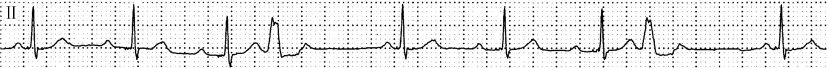
\includegraphics[width=3.09375in,height=0.94792in]{./images/Image00043.jpg}

\subsection{急诊处理原则和流程}

急性胸痛的急诊处理原则是:一是快速识别高危患者,以迅速进入快速救治绿色通道;剔除那些几乎没有或没有威胁生命疾病的患者;二是对不能明确诊断的患者应常规留院观察病情的演变,严防患者院外发生严重危及生命的事件。

1.首先判断病情严重性
,对生命征不稳定的患者,应立即开始稳定生命征的治疗;同时开始下一步处理;

2.对于生命征稳定的患者,首先获取病史和体征;

3.进行针对性的辅助检查;

4.在上述程序完成后能够明确病因的患者立即开始有针对性地病因治疗;

5.对不能明确病因的患者,建议留院观察,每隔30分钟复查一次心电图,每隔2小时复查心肌损伤标志物。心电图连续3次无变化,心肌损伤标志物连续2次无异常者在6~12小时后可予以出院。具体处理流程见图\ref{fig8-1}。

\begin{figure}[!htbp]
 \centering
 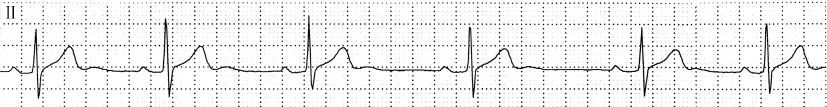
\includegraphics[width=4.69792in,height=5.41667in]{./images/Image00044.jpg}
 \captionsetup{justification=centering}
 \caption{胸痛的处理流程图}
 \label{fig8-1}
  \end{figure} 

\hypertarget{text00023.htmlux5cux23CHP1-8-4}{}
参 考 文 献

1. O'Connor R E,Bossaert L,Arntz H R,et al. Acute Coronary
Syndromes:2010 International Consensus on Cardiopulmonary Resuscitation
and Emergency Cardiovascular Care Science With Treatment
Recommendations. Circulation,2010,122: S422-S465.

2. Braunwald E,Antman E M,Beasley J W,et al. ACC/AHA Guideline Update
for the Management of Patients With Unstable Angina and Non-ST-Segment
Elevation Myocardial Infarction---2002:Summary Article:A Report of the
American College of Cardiology/American Heart Association Task Force on
Practice Guidelines(Committee on the Management of Patients With
Unstable Angina).Circulation,2002,106:1893-1900.

3. 罗学宏.急诊医学.北京:高等教育出版社,2008.74-78.

\protect\hypertarget{text00024.html}{}{}

\chapter{咯 血}

咯血(hemoptysis)是指喉腔、气管、支气管和肺组织出血,由咳嗽动作经口腔排出。咯血的临床过程难以预料,有时,初始仅少量痰中带血,却可以是大量的致命性咯血的先兆。大咯血引起失血性休克而致死的较少见,更常见的是大量的血淹溺肺泡,阻塞气道,因窒息和顽固性低氧血症而导致患者死亡。

咯血量可因病因和病变性质的不同而有差异,与病变的严重程度也不完全一致。临床上多根据咯血量将其分为少量咯血:24小时内咯血量≤100ml,包括痰中带血;中等量咯血:24小时内咯血量100~500ml;大咯血:24小时内咯血量>
500ml或一次咯血量≥200ml。大咯血约占全部咯血患者的1\%~4\%,但其死亡率高达80\%以上。

大咯血致死的危险与咯血量、出血速度、肺内潴留的血量以及患者基础肺功能储备相关,而与咯血的病因无关。年老体弱或久病无力者咳嗽乏力、基础肺功能差,即使几口血痰也可窒息致死。

\subsection{病因与发病机制}

\subsubsection{病因}

咯血的病因很多(表\ref{tab9-1}),但以肺结核、支气管扩张症、肺癌和肺炎等4种疾病多见。

尽管当今的检查手段有了长足的发展,对咯血患者采用了各种检查方法,但仍可有5\%~15\%的患者咯血原因不明,这类患者称隐匿性咯血(occult
hemoptysis)。部分隐匿性咯血可能由于气管、支气管的非特异性溃疡、静脉曲张、早期腺瘤、支气管小结石及轻微支气管扩张等病变引起。

\subsubsection{发病机制}

许多肺内外疾病和全身性疾病均可引起咯血,但咯血的机制有所不同。一般说来,炎症或肿瘤多导致病灶局部的毛细血管破坏,如不侵蚀支气管动脉,则咯血量一般较小。病变若侵蚀小动脉、小动静脉瘤或黏膜下静脉破裂则常常出现中等量或大咯血,而全身性疾病或严重而广泛的毛细血管炎症导致的咯血大多为中等量。小到中等量咯血大多可以自行终止,所以咯血很少引起失血性休克。

\begin{table}[htbp]
\centering
\caption{咯血的常见病因}
\label{tab9-1}
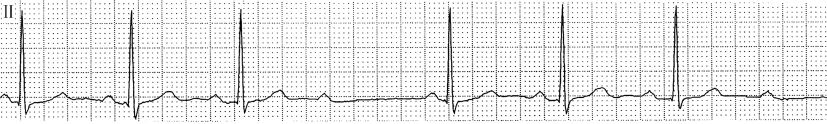
\includegraphics[width=6.59375in,height=3.875in]{./images/Image00045.jpg}
\end{table}

\subparagraph{气管、支气管疾病}

各种病原微生物如细菌、病毒、支原体、寄生虫以及肿瘤、各种粉尘、异物、结石等,均可侵蚀气道邻近血管或肺泡毛细血管导致咯血。支气管扩张导致的咯血常见,炎性病变侵蚀血管壁,使血管弹性纤维遭到破坏或在支气管壁下形成假性动脉瘤,当用力咳嗽时血管破裂导致大咯血;癌组织可直接侵蚀血管壁破裂导致咯血,少到痰中带血,多到大咯血窒息均可发生。

\subparagraph{肺部疾病}

许多肺部病变可直接侵蚀血管致使破裂出血或肺毛细血管床广泛损伤出血。大咯血最常见于肺结核(尤见于空洞性肺结核)、急性肺脓肿、癌性坏死及空洞形成、肺囊肿继发感染等,其穿行的支气管动脉或肺动脉受蚀,或动脉壁肌纤维破坏形成假性动脉瘤因咳嗽而破裂出血。此类咯血可因血凝块暂时充填空洞而压迫血管暂停出血,但也可因血凝块自溶而再次出现咯血。慢性肺脓肿多引起小量咯血,偶有大咯血发生。

\subparagraph{肺血管病变或先天性病变}

支气管动脉-肺动脉瘘是由于肺动脉因体循环压力,形成动脉瘤,破溃出血。肺动脉栓塞、多动脉炎、白塞病的病变基础多为栓塞性动脉炎或动脉瘤样扩张。夹层动脉瘤或梅毒性动脉瘤,偶与支气管动脉相通,可造成致命性大咯血。原发性肺动脉高压可因肺动脉远端阻力加大,肺动脉与肺毛细血管形成侧支循环,当血管破裂时引起咯血。偶见于先天性肺动-静脉瘘,先天性毛细血管扩张症引起的咯血。

\subparagraph{心血管疾病}

最常见的原因是二尖瓣狭窄和冠心病、心肌病等疾病导致的急性左心功能不全。左房血流受阻造成左房压力高,心脏前负荷增加,肺毛细血管及肺静脉压力升高,导致肺血管扩张,肺处于淤血状态,可引起肺水肿,并导致支气管黏膜下小静脉曲张,常自发或在炎症诱发下引起小静脉及毛细血管破裂,导致大咯血。

\subparagraph{全身性疾病}

脓毒症、肾出血-出血热综合征、出血型钩端螺旋体病等急性全身感染性疾病、血液病和某些自身免疫性疾病如大动脉炎、白塞病、系统性红斑狼疮、肺出血-肾炎综合征(Goodpasture
syndrome)、子宫内膜异位症等病变,使肺微血管和毛细血管受损,血管内皮细胞功能障碍,血管脆性增加以及血小板减少或功能障碍导致出血。此类咯血多为弥漫性肺泡出血。

\subparagraph{出凝血机制障碍}

包括血液系统疾病及DIC所致的咯血,多为全身多脏器出血的一部分。多见于全身性疾病导致的血小板减少和(或)功能障碍、凝血因子缺乏和(或)功能异常。此类咯血为原发病的继发性改变,罕见情况下咯血可能为首发症状。

\subsection{诊断思路}

多数咯血患者为突然起病,尤其第一次见到咯出鲜血,精神高度紧张,甚至有恐惧感,往往不能正确的诉说相关的症状及所见到血液的性状。因此,明确出血部位和出血原因显得尤为重要。

\subparagraph{确定出血部位}

口腔、鼻腔、咽喉部以及消化道出血有时可误认为咯血,特别是后鼻道出血多流入口腔或食管出血未经胃酸作用直接呕出时,有时会出现刺激性咳嗽而导致对出血部位判断的错误,即所谓的“假性咯血”(pseudo-hemoptysis)。对首次从口腔内咳或呕血者,在不能判断出血部位的情况下,应仔细寻找出血部位。对可疑鼻咽部出血者,应迅速邀请专科会诊以明确诊断。详细询问病史和仔细的体格检查多能明确。呕血在大多数情况下诊断并无困难,在临床上可依据临床表现、体格检查、辅助检查和实验室检查予以区别。

\subparagraph{临床表现特点}

除有原发病症状与体征外,大多数情况下,患者咯血前常有喉部痒感,血呈弱碱性,色鲜红,呈泡沫状,多混有痰液,咯血后数天内仍可咳出血痰。常见咯血病因的临床表现特点见表\ref{tab9-2}。

\begin{table}[htbp]
\centering
\caption{常见咯血原因的临床表现特点}
\label{tab9-2}
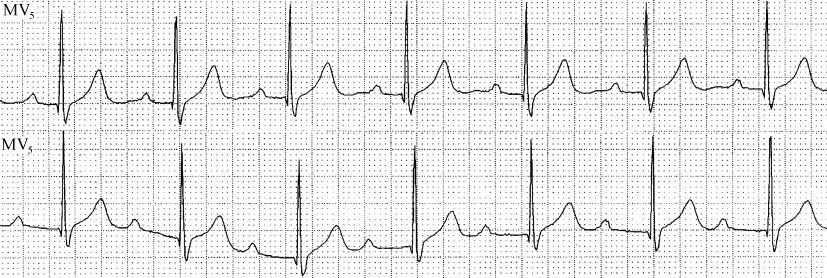
\includegraphics[width=3.26042in,height=2.38542in]{./images/Image00046.jpg}
\end{table}

大量咯血可引起急性出血性休克而出现面色苍白、冷汗、四肢湿凉,血管充盈度下降,血压降低等表现。因血凝块阻塞气道出现窒息的特征为咯血量突然减少或停止,同时出现胸闷、双手抓胸、喉头异常作响、继而烦躁不安、表情呆滞或恐惧、目瞪口张、全身发绀、呼吸变浅、速率加快,大小便失禁,肺部检查可见一侧或双侧呼吸音消失,进而呼吸突然停止。其他还包括肺不张和肺部继发感染等并发症的临床表现。

\subparagraph{咯血与呕血的鉴别}

大量呕血时,鲜红色血液可从口腔及鼻腔涌出,或大咯血时部分血液咽下,复又呕出,致使咯血与呕血不宜鉴别。正确的鉴别诊断有助于采取恰当的治疗措施。咯血与呕血的鉴别见表\ref{tab9-3}。

\begin{table}[htbp]
\centering
\caption{咯血与呕血的鉴别}
\label{tab9-3}
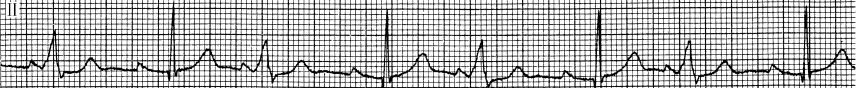
\includegraphics[width=3.26042in,height=2.05208in]{./images/Image00047.jpg}
\end{table}

\subparagraph{辅助检查与实验室检查}

\hypertarget{text00024.htmlux5cux23CHP1-9-2-4-1}{}
(1) 影像学检查:

胸部X线可初步判断胸部病变的性质和部位。胸部CT检查有助于支气管、肺部和胸腔疾病的病因诊断。尤其是高分辨CT(HRCT)可显示次级肺小叶为基本单位的细微结构,可明确病变的性质及范围,基本上已代替支气管造影。HRCT及核素扫描可明确心肺血管病变及占位性病变。必要时可作支气管动脉造影,但一般仅用于介入治疗前对出血部位的精准定位。

\hypertarget{text00024.htmlux5cux23CHP1-9-2-4-2}{}
(2) 超声与心电图检查:

心脏彩色多普勒与心电图检查对心脏病变诊断有帮助,可发现各种类型心脏结构改变、心律失常、ST-T段等改变。腹部B超有助于了解肝、脾、腹水、腹腔肿物等情况。

\hypertarget{text00024.htmlux5cux23CHP1-9-2-4-3}{}
(3) 血常规及生化检查:

可见白细胞总数增加,以中性粒细胞增加为主时提示感染存在。出血较多时可见红细胞和血红蛋白含量下降,血小板可正常。凝血功能、肝功能、肾功能等异常均能对其原发病提供参考。血气分析有助于发现病情较重患者的低氧血症。

\hypertarget{text00024.htmlux5cux23CHP1-9-2-4-4}{}
(4) 痰液检查:

细菌、真菌和细胞学检查有助于原发病的诊断和治疗。

\hypertarget{text00024.htmlux5cux23CHP1-9-2-4-5}{}
(5) 特异性检查:

如结核菌素试验、免疫学检查有时会对结核病、结缔组织疾病的诊断具有重要参考价值。

\hypertarget{text00024.htmlux5cux23CHP1-9-2-4-6}{}
(6) 纤维支气管镜检查:

可发现部分患者的出血部位和性质,并可在镜下止血,同时还可进行局部灌洗、标本取样做病原学和细胞学检查。

\hypertarget{text00024.htmlux5cux23CHP1-9-2-4-7}{}
(7) 动脉造影:

支气管动脉造影可显示区域性支气管动脉异常,确定出血部位,是决定进行栓塞治疗的主要依据。肺动脉造影对来自肺动脉的大咯血,尤其是支气管动脉栓塞后继续出血者适用。对空洞性肺结核或其他肺化脓性疾病、疑Rasmussen动脉瘤或肺动静脉瘘所致的咯血,选择性支气管动脉及肺动脉造影应同时进行,若病变波及双重动脉系统,则可以同时作栓塞治疗,以免术后继续出血。

\subparagraph{常见疾病鉴别诊断}

通过询问与咯血相关的病史、诱因、咯血量和伴随症状以及详细的体格检查多能寻找到原发疾病的线索。体格检查应注意有无肺部啰音、皮肤黏膜有无出血、淋巴结是否肿大、有无肝脾肿大、心脏杂音及体重减轻等。出血部位的判断可根据肺部体征及X线检查确定。

\hypertarget{text00024.htmlux5cux23CHP1-9-2-5-1}{}
(1) 支气管扩张:

缓慢起病,反复咳嗽伴脓痰和(或)量不等的咯血。既往多有麻疹、肺炎或免疫缺陷等病史。部分患者咯血为唯一症状,即所谓的“干性支气管扩张”。部分患者表现为反复发生的同一肺段感染,并迁延不愈,查体可闻及患侧固定而持久的湿啰音,可见杵状指(趾)等。胸部X线摄片或CT均可明确诊断。

\hypertarget{text00024.htmlux5cux23CHP1-9-2-5-2}{}
(2) 肺结核:

活动期多有午后低热、乏力、食欲减退、盗汗等结核中毒症状,部分可有不规则性高热。痰检或培养结核分枝杆菌阳性。查体可见结核面容、消瘦,局部湿啰音等。胸部X线摄片或CT表现多种形态,如局部渗出、增殖、纤维化、干酪性病变、钙化或空洞形成,以肺上叶尖后段及后基底段多见,可伴有胸腔积液、胸膜肥厚与粘连。聚合酶链反应(PCR)及结核菌素纯蛋白衍生物实验(purified
protein
derivative,PPD)有助于确定诊断,但后者不能区分是自然感染还是卡介苗免疫反应。

\hypertarget{text00024.htmlux5cux23CHP1-9-2-5-3}{}
(3) 肺癌:

持续出现咳嗽、咳痰,不明原因体重下降,近期痰中带血,反复出现。晚期可出现与呼吸运动有关联的胸痛及血性胸腔积液。查体可见气促、肺局限性喘鸣音、呼吸音增强或单侧胸腔积液、转移性骨压痛、淋巴结肿大(以颈部、腋窝为主,右锁骨上窝淋巴结肿大具有特殊诊断意义)等。胸部X线摄片或CT有助于诊断,痰液细胞学及活检可明确诊断。

\hypertarget{text00024.htmlux5cux23CHP1-9-2-5-4}{}
(4) 肺脓肿:

急性起病,多有劳累、受凉等病史。高热伴有不同程度的咯血。发病两周左右突然咳出大量脓痰及坏死组织,痰咳出后,体温下降。查体可发现局部湿啰音,偶可闻及空瓮音,宜可见杵状指(趾)。胸部X线摄片或CT和痰液细菌培养阳性多能明确诊断。

\hypertarget{text00024.htmlux5cux23CHP1-9-2-5-5}{}
(5) 风湿性二尖瓣狭窄:

有风湿性心脏病史。常在感冒、活动后出现呼吸困难,严重时不能平卧,常出现急性左心功能不全表现,伴以咳出大量粉红色泡沫样痰。小量咯血多见,偶见大量咯血。查体可见“二尖瓣面容”,心尖部听诊可及第一心音亢进、开瓣音、舒张中晚期隆隆样杂音、肺动脉瓣区第二心音亢进等,部分患者可摸到舒张期震颤。心脏多普勒超声检查可明确诊断。

\hypertarget{text00024.htmlux5cux23CHP1-9-2-5-6}{}
(6) 急性肺梗死:

有长期卧床、骨折、静脉炎或心房纤颤等病史。突然出现胸痛、胸闷、心悸、烦躁、冷汗,甚至晕厥,以小~中等量咯血多见。查体可见呼吸加快,肺局部叩诊浊音、呼吸音减弱及干湿性啰音。严重者可见急性右心衰表现,如心率加快、肺动脉瓣第二心音亢进、三尖瓣区可闻及收缩期杂音,可伴心律失常。血压下降,颈静脉怒张,肝脏增大、肝颈征阳性等。D-二聚体阳性及胸部X线摄片或CT有助于诊断。

\hypertarget{text00024.htmlux5cux23CHP1-9-2-5-7}{}
(7) 其他咯血的病因诊断:

其他一些肺部或全身性病变引起的咯血,根据发病特点和辅助诊断特征,大多数诊断并不是很困难。重要的是要想到一些引起咯血的少见原因,如肺血管畸形、血液病、结缔组织病、肺肉芽肿症、遗传性毛细血管扩张症、肺出血-肾炎综合征、经期性咯血等。弥漫性肺泡出血诊断的最好方法是通过灌洗获得肺泡巨噬细胞中的含铁血黄素来确定。目前ICU中出现的咯血日益增多,大多数为弥漫性肺泡出血,少部分为设备使用或操作不当导致的大咯血,应引起足够重视。

咯血病因诊断流程见图\ref{fig9-1}。

\subsection{病情评估}

咯血患者出现下列情况表明病情危重:咯血量较大,一次超过200ml,反复发作,一般止血措施不能控制;精神高度紧张或恐惧,呼吸困难、胸闷,双手无目的抓挠喉或胸部,表明出现窒息先兆;短期内即出现失血性休克表现;胸部X线片(或CT扫描)提示空洞或可疑病变侵及小动脉及假性动脉瘤破裂。

\subsection{处理原则}

咯血的急诊治疗取决于速度与量。大咯血抢救的重点在于迅速有效止血,保持呼吸道通畅,防治窒息及其他并发症,并同时进行病因、对症治疗。

\subsubsection{窒息的紧急处理}

咯血窒息是导致患者死亡的主要原因,应及早识别和抢救。窒息抢救的重点是保持呼吸道通畅和纠正缺氧。

\begin{figure}[!htbp]
 \centering
 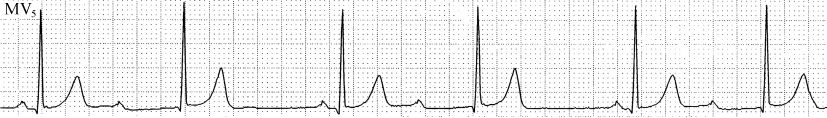
\includegraphics[width=4.55208in,height=5.47917in]{./images/Image00048.jpg}
 \captionsetup{justification=centering}
 \caption{咯血病因诊断流程图}
 \label{fig9-1}
  \end{figure} 

1.体位
患侧卧位,避免血液流向健侧。头低位,身体与床成40°~90°角,背部屈曲并拍击背部,促进肺内血液流出。病灶不明确者可暂取平卧位。同时清除口腔内血块。

2.保持呼吸道通畅
用导管自鼻腔插至咽喉部,用吸引器吸出血液(块),并刺激咽喉部,使患者用力咯出堵塞于气管内的血液(块),或在直接喉镜下作硬质支气管镜直接插管,通过冲洗和吸引,迅速恢复呼吸道通畅。

3.建立静脉通道 迅速建立静脉通道,补充血容量,使用止血药物,纠正休克。

4.镇静 根据病情需要,可适量给予镇静药物,如地西泮、氯丙嗪等。

5.机械通气 高浓度给氧(FiO\textsubscript{2}
30\%~40\%)或高频通气治疗。如自主呼吸微弱或消失,应立即进行气管插管或切开使用机械通气治疗。

6.若自主呼吸极弱或消失
,则应立即进行心肺复苏。在呼吸道通畅情况下同时使用呼吸兴奋剂。窒息解除后应及时对复苏后并发症进行处理,如纠正酸中毒、补充血容量、控制休克以及重要器官功能的监测与支持,如治疗和预防脑水肿、心肺功能不全、肾功能不全等。

大咯血患者应绝对卧床,尽量避免搬动或转送他院,颠簸可加重咯血,甚至导致死亡。如需转送,途中应将患者的头和身体偏向患侧或俯卧头低位,以利引流,防止窒息。密切观察患者的生命体征,包括意识、呼吸、脉搏和血压,随时做好抢救准备工作,尽可能准确记录咯血量。

\subsubsection{急诊处理}

\subparagraph{镇静 、休息与对症处理}

少量咯血,如痰中带血,一般无需特殊处理,适当减少活动量,对症治疗即可。中等量咯血应卧床休息;大量咯血则应绝对卧床休息。取患侧卧位,患侧可放置冰袋,嘱患者将血轻轻咳出,避免吸入性肺炎、肺不张或以防窒息,出血部位不明时取平卧位。对精神紧张、恐惧不安者,应解除不必要的顾虑,必要时可给少量镇静药,如地西泮(安定)10mg或苯巴比妥钠0.1~0.2g肌注,或口服地西泮、氯氮{}
(利眠宁)等。鼓励患者咳出滞留于呼吸道的陈血,避免呼吸道阻塞。对频咳或剧咳者,可给镇咳药如喷托维林(pentoxyverine,咳必清)25mg,每天3次;可待因15~30mg,每天3次或二氧丙嗪(克咳敏)5mg,每天3次口服。但大咯血时一般不用镇咳剂,如剧咳妨碍止血,可在血液咳出后临时使用可待因15~30mg口服或皮下注射,每日1~3次;对年老体弱、肺功能不全者不宜用,禁用吗啡、哌替啶等,以免过度抑制咳嗽,使血液及分泌物淤积气道,引起窒息。

\subparagraph{严密观察与护理}

进食易消化食物,保持大便通畅,避免用力屏气排便。对大、中量咯血者,应密切观察患者,做好大咯血与窒息的各项抢救准备,定期记录咯血量、测呼吸、脉搏和血压,若有口渴、烦躁、厥冷,面色苍白、咯血不止或窒息表现者,应立即进行抢救。

\subparagraph{止血药物的应用}

常用止血药物有:

\hypertarget{text00024.htmlux5cux23CHP1-9-4-2-3-1}{}
(1) 垂体后叶素(pituitrin):

疗效迅速而显著,使肺循环压力降低,肺小动脉收缩而利于血凝块形成。用法:大咯血时以垂体后叶素5~10U加25\%葡萄糖液20~40ml缓慢静脉注射(10~15分钟);咯血持续者可用垂体后叶素10~20U加5\%葡萄糖液500ml,缓慢静滴;禁用于高血压、冠状动脉疾病、肺源性心脏病、心力衰竭患者和孕妇。注射过快可引起面色苍白、心悸、出汗、胸或腹痛、血压升高等副作用,应及时减慢速度或停药。

\hypertarget{text00024.htmlux5cux23CHP1-9-4-2-3-2}{}
(2) 普鲁卡因(procaine):

用于对垂体后叶素有禁忌者。普鲁卡因150~300mg加5\%葡萄糖液500ml缓慢静滴,或普鲁卡因50mg加25\%葡萄糖液40ml,缓慢静注。本药可诱发过敏反应,用药前应作皮试。药物使用量过大或注射过快,可导致惊厥、谵妄、兴奋、面色潮红,应立即停药,对症处理。

\hypertarget{text00024.htmlux5cux23CHP1-9-4-2-3-3}{}
(3) 酚妥拉明:

为α-肾上腺素能受体阻滞剂,能有效扩张血管平滑肌,降低肺循环阻力及心房压、肺毛细血管楔压和左心室充盈压,可起到较好的止血作用。酚妥拉明10~20mg加入5\%葡萄糖液250~500ml中持续静滴。使用时监测血压并保持有足够的血容量。

\hypertarget{text00024.htmlux5cux23CHP1-9-4-2-3-4}{}
(4) 纠正凝血障碍药物:

①6-氨基己酸(氨己酸,EACA):6.0g +
5\%葡萄糖液250ml静滴,通过抑制纤维蛋白溶酶形成达到止血目的,适用于肺部疾病、血液病引起的咯血。②氨甲苯酸(对羧基苄胺,PAMBA):100~200mg
+ 25\%葡萄糖液40ml静滴,或200mg +
5\%葡萄糖液500ml静滴,适用于纤维蛋白溶解亢进引起的出血。③氨甲环酸(AMCA):AMCA
250mg + 25\%葡萄糖液40ml静注;或AMCA 750mg +
5\%葡萄糖液500ml,静脉滴注。④肾上腺色腙(安络血):通过抑制毛细血管通透性、增加毛细血管抵抗和加速管壁回缩发挥止血作用。10~20mg肌肉注射,1日2次,或5mg
1日3次口服。⑤酚磺乙胺(止血敏):有收缩肺毛细血管、增加毛细血管抵抗、加速管壁回缩及轻微的促血小板聚集作用。0.25~0.75g肌肉注射或缓慢静脉注射,1日2~3次,静脉注射不宜过快,以免血压下降。⑥注射用血凝酶(立止血):该药对纤维蛋白原的降解有选择性作用,在出血部位生理性凝血因子的作用下,纤维蛋白多聚体迅速形成稳固的纤维蛋白,在出血部位发挥凝血作用。1~2U静脉注射或肌肉注射,1日1~2次。

\hypertarget{text00024.htmlux5cux23CHP1-9-4-2-3-5}{}
(5) 其他止血药物:

硝酸甘油适用于与垂体后叶素合用,5~10mg加入5\%~10\%葡萄糖液250~500ml中静滴;氯丙嗪能降低肺循环、左心室与支气管动脉压力,必要时可小剂量(10~15mg)配合使用,肝、肾功能不全者慎用。另外,阿托品、654-2、高渗氯化钠、糖皮质激素、中药如白连粉、三七粉、云南白药等、鱼精蛋白注射液、维生素C、凝血酶原复合物等根据病情均可酌情选用。

\subparagraph{维持血容量}

持续大咯血出现循环容量不足时应及时补充血容量。输注新鲜血不但能补充血容量外,而且还有止血作用。

\subparagraph{手术止血}

对反复咯血,上述治疗无效,出血部位明确而无手术禁忌者,可采用手术止血。指征包括:①肺部病变(如各型结核动脉破裂、支气管扩张、肺脓肿、肺癌等)所引起的致命性大咯血;②可能发生气道阻塞和(或)窒息者。

\subparagraph{局部止血治疗}

适用于大咯血并发窒息和严重反复咯血、病情严重、肺功能较差、不适于手术治疗者。前提是出血部位明确,经气管插管或支气管镜边插边吸,到达出血部位后,将导管由活检孔插入至出血部位,注入冷生理盐水(4℃),每次50ml,留置30~60秒种后吸出,反复数次,直至出血停止,通过冷刺激使血管收缩达到止血的目的;或者注入凝血酶200~400U,或去甲肾上腺素液1~2mg稀释后局部使用。

\subparagraph{支气管动脉栓塞}

对药物治疗无效且不能手术治疗的患者,是可选择的治疗方法之一。经股动脉插管,将漂浮导管插到病变区域支气管动脉分支的血管腔内,注入明胶海绵或聚乙烯醇微粒(直径0.5~2.0μm),栓塞支气管动脉,以达到止血目的。因肺循环可能有多支动脉供血,本法对不是来自支气管动脉(侧枝血管)破裂的咯血无效,而且造影剂和栓塞物还可能进入脊髓动脉,引起脊髓缺血损伤,因此应严格掌握适应证。

\subparagraph{肺不张和肺炎的治疗}

采用体位引流(侧卧位,患侧在上),雾化吸入,使用解痉药、祛痰药,应用抗生素预防和控制感染。

\subparagraph{病因治疗}

尽快明确病因,采用相应治疗措施。

\protect\hypertarget{text00025.html}{}{}

\hypertarget{text00025.htmlux5cux23CHP1-9-5}{}
参 考 文 献

1. Parrillo,Dellinger. Critical Care Medicine:Principles of Diagnosis
and Management in the Adult. 3th ed. Elsevier Inc,2008

2. Stone CK,Humphries. Current Emergency Diagnosis and Treatment. 5th
ed. New york:Lange/McGraw,2004

3. John A Marx. Rosen's Emergency Medicine. Concepts and Clinical
Practice. 6th ed. St. Louis:Mosby Inc,2006

4. 徐腾达,于学忠.现代急症诊断治疗学.北京:中国协和医科大学出版社,2007

5. 沈洪.急诊医学.北京:人民卫生出版社.2007

\protect\hypertarget{text00026.html}{}{}

\chapter{急 性 腹 痛}

腹痛(abdominal
pain)是指由于各种原因引起的腹腔内外脏器的病变,而表现在腹部的疼痛。可分为急性与慢性腹痛两类。急性腹痛(简称急腹痛)是临床最常见急症之一,其病因繁杂,病情多变,涉及学科广,内、外、妇产、儿及传染病等科疾病均可引起,诊断处理不当,常可造成恶果,因而对急性腹痛必须尽快作出定位、定性及病因诊断,以防误诊、漏诊及误治,从而改善预后。对生育期女性的急性腹痛须请妇产科医生会诊,以排除妇产科急腹症。

\subsection{病因与发病机制}

\subsubsection{病因}

引起腹痛的病因颇多,大体可分为腹腔内脏器疾病及腹腔外脏器疾病两大类,每类又可分为器质性病变及功能性失调;器质性病变包括脏器的急性炎症、损伤、破裂、穿孔、梗阻、扭转、出血、坏死等;功能性失调有痉挛、麻痹、神经功能紊乱及功能暂时性失调等(详见表\ref{tab10-1})。

\subsubsection{发病机制}

腹痛依发生机制分为三型,即真性内脏痛(true visceral
pain,内脏痛):由内脏本身病变所致;类似内脏痛(somatic
pain,体性痛,体壁性内脏痛):由内脏病变累及壁层腹膜,经躯体神经传入引起疼痛;放射痛(referred
pain,牵涉痛):内脏病变引起某一局部疼痛,痛处常非病变部位。

\subparagraph{内脏痛}

多由消化道管壁平滑肌突然痉挛或强力收缩,管壁或脏器突然扩张,急性梗阻、缺血等刺激内脏传入神经末梢产生冲动所致,常为脏器本身的疼痛。

\subparagraph{体性痛}

壁层腹膜分布着脊髓性感觉神经,脏层腹膜上虽无感觉受体,但近脏器的肠系膜、系膜根部、小网膜及膈肌等均有脊髓性感觉神经,当脏器病变累及其感觉神经时产生冲动,经上行传导达丘脑,再经交换神经元达大脑皮质。丘脑可感知疼痛,大脑可识别疼痛的部位、程度和性质。故体性痛多剧烈,疼痛及压痛部位明确,与体位有关,变换体位常可使疼痛增重。

\subparagraph{放射痛}

亦称牵涉痛或感应性痛。由于某种病理情况致身体某一局部发生疼痛,且痛处常非病变所在,此因放射痛部位与病变脏器的感觉常来自同一节段神经纤维。放射痛的特点为常伴有Head皮肤感觉过敏带(内脏皮肤过敏带)及腹壁紧张。

Head皮肤过敏带即腹腔内脏器疾病的病理性冲动,刺激内脏神经经交感神经传入相应或同一脊髓段的后根,由此发出的脊神经产生感应,将冲动传到体表一定部位致皮肤相应节段感觉过敏性疼痛,或引起远隔部位脏器痛。如胆绞痛向右肩背部放射;小肠绞痛放射到脐周;胃、十二指肠病变可放射到剑脐间等。

\begin{table}[htbp]
\centering
\caption{急性腹痛的病因分类}
\label{tab10-1}
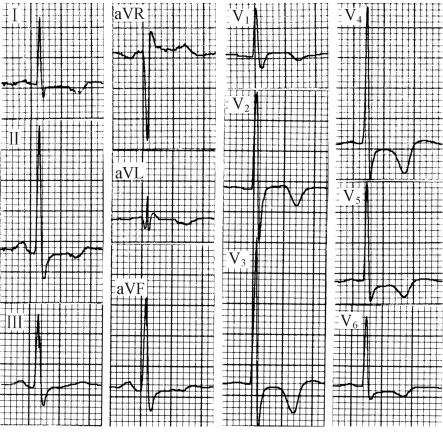
\includegraphics[width=6.67708in,height=3in]{./images/Image00050.jpg}
\end{table}

\subsection{诊断思路}

\subsubsection{病史及体检}

准确而简要的病史询问,全面而有重点的体检,对急性腹痛的诊断十分重要。

\hypertarget{text00026.htmlux5cux23CHP1-10-2-1-1}{}
(一) 年龄、性别、既往史

\subparagraph{年龄 、性别}

不同年龄及性别常有不同的多发病,如婴幼儿多见先天性消化道畸形,尤其是胃肠道(肠闭锁或狭窄,肛门闭锁、先天性肥厚性幽门狭窄等)及胆道(先天性胆道闭锁或狭窄);幼儿多见肠寄生虫病、肠套叠、疝嵌顿等;青壮年多见急性阑尾炎、胃肠穿孔、肠梗阻、腹部外伤致脏器破裂内出血等;老年人则胃肠道癌肿及并发症(穿孔、梗阻、出血),胆结石或胆囊炎及血管疾病多见。急性胆道疾病、胰腺炎女多于男,溃疡病穿孔、急性阑尾炎及肠梗阻则男多于女。引起急性腹痛的妇产科疾病,如急性附件或盆腔炎,异位妊娠或破裂,卵巢囊肿蒂扭转,子宫破裂、穿孔等及痛经。

\subparagraph{既往史}

应重点询问以往有否引起急性腹痛的病史,有无类似发作史;手术史、月经生产史、外伤史及有害物接触史等。

\hypertarget{text00026.htmlux5cux23CHP1-10-2-1-1-2-1}{}
(1) 有类似发作史者:

应考虑胆石症、胆囊炎、泌尿系结石、慢性阑尾炎或慢性胃炎急性发作,溃疡病活动或出血、穿孔,疝反复嵌顿,胃肠神经症等。

\hypertarget{text00026.htmlux5cux23CHP1-10-2-1-1-2-2}{}
(2) 手术史:

溃疡病胃次全切除术后吻合口溃疡、出血或狭窄,肠粘连或粘连性肠梗阻,膈下或盆腔脓肿等。

女性患者应注意有无痛经史,闭经且发生急性腹痛者应考虑异位妊娠、早期流产,若伴休克,应高度疑及异位妊娠破裂内出血等。

\hypertarget{text00026.htmlux5cux23CHP1-10-2-1-2}{}
(二) 注意腹腔内、外疾病所致急性腹痛的不同特点

\subparagraph{腹腔内疾病急性腹痛的特点}

①常伴有消化道症状,如恶心、呕吐、腹泻、腹胀等。②常有与进食有关的诱因,如暴饮暴食、高脂饮食、酗酒、进食过刺激、不洁或变质食物等。③腹部体征较明显且固定(痛、压痛、叩痛、反跳痛等)。④无腹外及全身疾病表现。

\subparagraph{外科或妇产科疾病所致急性腹痛的特点}

①腹痛突然发作,剧烈,急剧发展,不及时处理,短期内病情常迅速恶化。②表情痛苦,呻吟,大汗,面色苍白,辗转不安或蜷曲静卧。③可有腹膜刺激征(腹肌紧张呈板状,压痛、反跳痛明显)及肝浊音界缩小或消失。④可有内出血综合征,如头晕、心慌、多汗、面色苍白、脉细速、血压下降等。⑤急诊腹透可见膈下游离气体、高度胀气、鼓肠或胃扩张、梯形液气平面等。⑥发病短期内白细胞明显增高,中性及杆状核增高,中毒血象,进行性贫血等。

\subparagraph{内科腹腔脏器疾病所致急性腹痛的特点}

①腹痛可轻可重,短期内病情不恶化。②症状与体征不一致,主观感觉腹痛剧烈,表情痛苦,但检查腹部体征不显著,多腹软,局部轻压痛或压痛,无反跳痛。③发病短期内血象正常或稍高,无中毒血象。④急诊腹透无阳性发现。

\hypertarget{text00026.htmlux5cux23CHP1-10-2-1-3}{}
(三) 依急性腹痛部位诊断

即依据解剖部位来推断可能的病因(表\ref{tab10-2})。最早发生腹痛及压痛最明显的部位常是发生病变的部位(早期及异位阑尾炎例外)。

\hypertarget{text00026.htmlux5cux23CHP1-10-2-1-4}{}
(四) 依病史、体征及伴随症状综合分析

\subparagraph{起病方式}

突然发作剧痛,多为胆道蛔虫症、胆道或泌尿道结石嵌顿、疝嵌顿、急性胆囊炎或胰腺炎、消化道急性穿孔、腹腔脏器破裂、急性心肌梗死、心绞痛等。持续性腹痛阵发性加重常示有痉挛或梗阻;初期呈进行性加重多为急性炎症;暴饮暴食、高脂饮食、酗酒、过刺激或不洁食物、激烈运动等诱发急性腹痛应考虑急性胆囊炎、胰腺炎或胃肠炎,溃疡病穿孔,肠或卵巢囊肿蒂扭转,疝嵌顿等。

\subparagraph{绞痛及放射痛}

\begin{table}[htbp]
\centering
\caption{急性腹痛部位与疾病关系}
\label{tab10-2}
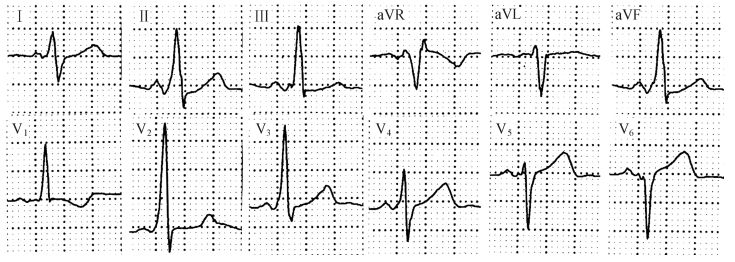
\includegraphics[width=6.71875in,height=3.52083in]{./images/Image00051.jpg}
\end{table}

①胆绞痛:右上腹痛向右肩胛及右背部放射。②胰腺绞痛:上腹或中上腹部向左侧腰背部放射。③小肠绞痛:脐周剧痛。④肾绞痛:肾区痛沿腹直肌外缘向大腿内侧或会阴部放射。⑤子宫或直肠病变绞痛:腰骶部或下腹部剧痛或坠痛。

\subparagraph{伴发症状}

\hypertarget{text00026.htmlux5cux23CHP1-10-2-1-4-3-1}{}
(1) 伴发热:

①先发热后腹痛多为不需手术治疗的内科性疾病(常为急性炎症)。②先腹痛后发热的多为外科或妇产科疾病,且常需手术治疗(如急性消化道穿孔、腹膜炎、肠梗阻、异位妊娠破裂、内脏破裂出血等)。③急性腹痛伴寒战、高热,应考虑急性化脓性胆囊炎、胆管炎,腹腔或腹内脏器的化脓性病变(膈下或盆腔脓肿、化脓性腹膜炎),下肺炎症或脓肿等。

\hypertarget{text00026.htmlux5cux23CHP1-10-2-1-4-3-2}{}
(2) 伴呕吐:

急性腹痛伴呕吐者常为急性胃、胆囊、胰腺等炎症,肠梗阻,胆道或泌尿道结石嵌顿,胃型感冒,肠套叠,痛经,神经症等。

\hypertarget{text00026.htmlux5cux23CHP1-10-2-1-4-3-3}{}
(3) 与排便的关系:

①腹痛伴腹泻:急性肠炎、痢疾、急性盆腔炎、急性阑尾炎、高位肠梗阻等。②腹痛伴血便:绞窄性肠梗阻、肠套叠、溃疡性结肠炎、坏死性肠炎、缺血性疾病(栓塞或血栓形成)等。③腹痛伴便秘或停止排便及肛门排气:为习惯或非习惯性便秘、肠梗阻等。

\hypertarget{text00026.htmlux5cux23CHP1-10-2-1-4-3-4}{}
(4) 伴腹胀:

急性胃扩张、麻痹性肠梗阻、便秘、尿潴留等。

\hypertarget{text00026.htmlux5cux23CHP1-10-2-1-4-3-5}{}
(5) 伴黄疸:

①右上腹痛伴黄疸者多为肝、胆系统疾病(炎症、结石、肿瘤等)。②中上腹或左中上腹痛伴黄疸多为胰腺(炎症、结石、肿瘤)或脾脏病变(脾梗死)。③右上腹痛伴寒战、高热、黄疸,应考虑急性胆囊炎,胆结石嵌顿伴炎症,急性化脓性胆囊、胆管炎,急性肝脓肿及少数膈下脓肿。

\hypertarget{text00026.htmlux5cux23CHP1-10-2-1-4-3-6}{}
(6) 与排尿关系:

腹痛伴膀胱刺激征或血尿者多为急性泌尿系感染、结石嵌顿;部分阑尾炎、盆腔脓肿也可引起膀胱刺激征,应注意鉴别。

\hypertarget{text00026.htmlux5cux23CHP1-10-2-1-4-3-7}{}
(7) 与体位的关系:

①辗转不安,腹痛喜按多为胃肠道疾病;拒按多为肝、胆系疾病。②活动疼痛加剧,蜷曲侧卧疼痛减轻多为腹膜炎。③前倾坐位或膝胸位疼痛减轻多为胰腺疾病。

\hypertarget{text00026.htmlux5cux23CHP1-10-2-1-4-3-8}{}
(8) 伴腹水:

①伴血性腹水:腹腔内脏或异位妊娠破裂,恶性肿瘤腹腔内转移,腹膜恶性肿瘤,少数结核性渗出性腹膜炎等。②脓性腹水:化脓性腹膜炎。③胰性腹水:乳糜状,浆液或浆液血性,淀粉酶含量增高且大于血中含量,蛋白量增高,对利尿剂及放腹水疗效差,见于急性出血坏死型胰腺炎或胰腺假囊肿破裂。④胆汁性腹水:化脓性胆囊炎或胆管炎破裂致胆汁性腹膜炎。

\hypertarget{text00026.htmlux5cux23CHP1-10-2-1-4-3-9}{}
(9) 伴休克:

应考虑下列疾病:①急性内出血:腹腔内脏器破裂或异位妊娠破裂。②急性穿孔致弥漫性腹膜炎。③腹腔内脏器或卵巢囊肿蒂扭转。④腹腔内急性血管性病变(肠系膜动脉栓塞或静脉血栓形成)。⑤急性心肌梗死或休克型肺炎。

\hypertarget{text00026.htmlux5cux23CHP1-10-2-1-4-3-10}{}
(10) 伴包块:

应考虑相应部位的急性炎症、肿瘤、肠套叠或扭转。

\hypertarget{text00026.htmlux5cux23CHP1-10-2-1-4-3-11}{}
(11) 与外伤关系:

急性腹痛发生前有外伤史者应考虑腹腔脏器破裂、内出血等。

\subsubsection{辅助检查}

\subparagraph{血液检查}

①血红蛋白及红细胞计数:可提示有无内出血致贫血(但早期由于脾脏及骨髓代偿性释放以及血液浓缩,可显示不出贫血或与临床实际贫血程度不符)。②白细胞计数及分类:可提示是否感染、感染程度等。

\subparagraph{大便检查}

外观:颜色、性状(成形、糊状、水样、血便、脓血便、黏液便或脓血黏液便等)。镜检:有无红、白细胞,虫卵、真菌、阿米巴滋养体等及潜血试验。

\subparagraph{尿液检查}

尿pH、蛋白、糖、酮体、胆红素、红细胞、白细胞、管型、细菌、真菌等,育龄女性应查尿妊娠试验。

\subparagraph{生化检查}

依病情需要可作:①血、尿淀粉酶测定;②血钾、钠、氯、钙,血糖,酮体等测定;③肝、肾功能测定等。

\subparagraph{心电图检查}

对40岁以上患者,既往无慢性胃病史,突然发作上腹痛应常规作心电图,以识别有无心脏及心包病变。

\subparagraph{X线检查}

①胸部X线检查:有助于肺炎、肺脓肿、肺癌、胸膜炎、气胸、肝或膈下脓肿等的诊断。②腹部X线检查:消化道急性穿孔致膈下游离气体,肠梗阻的梯形液气平面,急性胃扩张,高度鼓肠等。另外,胆道或泌尿道阳性结石等。

\subparagraph{超声波检查}

B超检查对肝、胆、胰、脾、肾、输尿管、子宫及其附件、盆腔、腹腔等探查均有较强分辨(实质性、囊性、良性、恶性、积液、结石等)及诊断能力,对胃肠道疾病可提供一定的诊断线索。

\subparagraph{内镜检查}

急诊内镜检查(胃、十二指肠、胆道、腹腔及结肠镜检查),对急性腹痛的诊断具有极其重要意义。可依临床初步拟诊病变部位,选择相应内镜检查,以助诊断及内镜直视下取活检或治疗。

\subparagraph{腹部}

CT检查
主要检查肝、胆、胰、脾、肾、膀胱、腹腔及盆腔等部位,可诊断其形态、大小、密度、占位性病变(实质性、囊性)、结石及腹腔、盆腔有无积液、肿大淋巴结等。

\subparagraph{诊断性腹腔穿刺术}

根据穿刺液性质可确定腹膜炎性质,有无内出血(脏器破裂或异位妊娠破裂)等。

\subparagraph{阴道后穹隆穿刺术}

主要用于判断异位妊娠破裂出血、盆腔脓肿或盆腔积液。

\subsubsection{急性腹痛的病因诊断线索}

急性腹痛的病因繁多。为尽早明确诊断,应在完成病史采集、体格检查和必要的辅助检查之后,对所得资料进行综合分析,作出正确的病因诊断。下述诊断思路,有助于最终确定病因诊断。

\hypertarget{text00026.htmlux5cux23CHP1-10-2-3-1}{}
(一) 确定是腹腔内病变或腹腔外病变

急性腹痛的诊断 ,首先要确定是腹腔内病变还是腹腔外病变。

\subparagraph{腹腔内病变}

常有消化道症状如恶心、呕吐、腹痛、腹泻等,腹痛程度不一,多有较明确诱因。腹部体征依病因而异,一般较明显,腹外与全身性症状轻微或缺乏。

\subparagraph{腹腔外病变}

胸部疾病引起的腹痛位于脐上的同侧腹部,可有压痛,但一般无反跳痛及肌紧张,胸部检查可发现有关疾病的心肺体征,胸部X线检查、心电图检查、心肌酶学检查等有助于诊断。全身性疾病所致的腹痛有原发病的表现,腹痛多由于电解质紊乱、代谢失调或毒素刺激所致,位于全腹或部位多变,一般无腹膜刺激征。

\hypertarget{text00026.htmlux5cux23CHP1-10-2-3-2}{}
(二) 确定是外科或非外科急性腹痛

\subparagraph{外科急性腹痛}

是指急需外科处理,或病情的发展有需要外科处理可能性的急性腹痛。对急性腹痛患者,应先明确是否为外科急性腹痛。此类腹痛常有以下特点:①剧烈而急起的腹痛多先于发热或呕吐,发热多于腹痛后4~6小时出现,但细菌性肝脓肿、脾脓肿和伤寒肠穿孔等例外。若腹痛超过6小时而患者体温反而降低或低于正常,则应考虑并发休克、大出血或严重感染毒血症的可能。②腹痛部位明确,有固定区,患者多“拒按”腹痛区。③常伴腹膜刺激征。腹痛、固定性压痛点和肌紧张的程度常是越来越严重,提示病变呈进行性发展。④腹式呼吸减弱或消失,肠鸣音亢进或消失,机械性肠梗阻时可闻及高调肠鸣音,而弥散性腹膜炎、麻痹性肠梗阻则肠鸣音减弱或消失。⑤可有肝肺浊音界消失,腹部移动性浊音阳性。⑥腹痛时腹部膨隆或可见胃肠型及蠕动波,并可触及腹部包块或索状物等。⑦腹腔穿刺可有血性或脓性液体等。

\subparagraph{内科急性腹痛}

其特点:①一般先有发热或呕吐、腹泻而后出现腹痛。②腹痛可轻可重,腹部体征不明显,无固定而局限性压痛点,无腹膜刺激征。患者常喜按。③腹式呼吸存在,肠鸣音正常或活跃。④可有与腹痛有关的内科疾病的阳性体征。⑤血白细胞正常或升高。

\subparagraph{妇产科急性腹痛}

其特点:①由于女性生殖器官集中于下腹部盆腔内,所以妇产科疾病引起的腹痛多局限于中下腹、盆腔,并向会阴和骶尾部放射。②腹痛多与月经、妊娠有关,月经期曾患过上呼吸道感染或有过性生活,多为急性盆腔炎;卵泡破裂多发生在排卵期;宫外孕有停经史,可有早孕反应等。③可伴有腹腔内出血、阴道出血或分泌物增加。④妇科检查常有阳性体征发现。

\subparagraph{小儿内科急性腹痛}

其特点:①常以发热、咽痛、咳嗽等症状先于腹痛。②急性腹痛而腹壁柔软,无压痛,腹部无包块、肠型等腹部体征。③腹痛范围广,不规则性,但排便基本正常。④可伴有呕吐等。⑤腹部外疾病引起腹痛者,可发现原发病变部位的阳性体征。

\hypertarget{text00026.htmlux5cux23CHP1-10-2-3-3}{}
(三) 确定急性腹痛的性质

根据常见的病变性质可将急性腹痛归纳为以下七类:

\subparagraph{炎症性急性腹痛}

基本特点为:腹痛+发热+压痛或腹肌紧张。

临床特点有:①一般起病较缓慢,多由轻渐重。②持续性腹痛。因脏器或腹膜的炎症、充血、水肿,刺激神经而引起急性腹痛,多呈持续性腹痛进行性加重。因发病的部位、病变程度及其病理变化不同,而呈局限性或全腹性疼痛。疼痛多发生于病变所在的部位。③当炎症病变波及脏器浆膜和壁层腹膜时,则呈典型的局限性或弥漫性腹膜刺激征,即腹肌紧张、压痛和反跳痛,尤其是以病变所在部位最明显。④早期可出现全身感染征象,如寒战、发热、脉快和白细胞增高。⑤腹腔穿刺和灌洗可抽出腹腔炎性渗出物。⑥可有明显的胃肠道刺激症状。此类急腹痛常见的有急性阑尾炎、急性胆囊炎、急性腹膜炎、急性胰腺炎、急性盆腔炎、急性肠系膜淋巴结炎、急性出血性坏死性肠炎等。

\subparagraph{穿孔性急性腹痛}

基本特点是:突发持续腹痛+腹膜刺激征,可伴有肠鸣音消失或气腹。

由外伤、炎症或癌肿侵蚀等导致空腔脏器破裂所致。其临床特点有:①突然剧烈的刀割样腹痛,后呈持续性,范围迅速扩大。②腹壁板样强直,有明显腹膜刺激征,常伴有休克。③常见膈下游离气体和腹部移动性浊音。④肠鸣音消失。例如消化性溃疡穿孔、胃癌穿孔、胆囊穿孔、伤寒肠穿孔、外伤性肠穿孔等。

\subparagraph{梗阻性急性腹痛}

基本特点是:阵发性腹痛+呕吐+腹胀+排泄功能障碍。

肠道、胆道、输尿管等空腔管道内结石、肿瘤和位置改变(如扭转、套叠)等因素阻塞,腔内压增高促使管腔道平滑肌强烈收缩以排除障碍,发展到血运障碍(如绞窄性疝等),或始发于血运障碍(如肠系膜血管阻塞等),继发缺血、坏死等变化,即发生梗阻性急腹痛。其临床特点有:①阵发性腹部剧痛是其特征,多突然发生,呈阵发性剧烈绞痛,往往使患者难以忍受。当梗阻器官合并炎症或血运障碍时,常呈持续性腹痛,阵发性加重。②恶心、呕吐,早期是反射性,后期是逆流性呕吐。因梗阻发生的部位不同,呕吐的内容和量亦不同。胃肠道高位梗阻则早发频吐,多为胃及十二指肠内容物;低位梗阻则晚发溢吐,严重者可呕吐粪性内容物。③腹胀和梗阻的器官管型明显,此因梗阻的器官、部位、程度和病变性质不同而表现亦异:如幽门梗阻表现上腹胀、振水音,可见胃蠕动波;肠梗阻可见腹胀、肠型、蠕动波;胆道梗阻出现胆囊肿大或胆管扩张;泌尿系梗阻出现膀胱区域或肾区的囊性肿块等。④正常排泄功能障碍。胃肠道梗阻出现呕吐、肛门停止排便排气;胆道梗阻出现黄疸;泌尿系梗阻则呈现尿少或尿潴留、肾积水等。⑤除泌尿系疾病外,多伴有水、电解质与酸碱平衡失调、休克,或晚期毒血症。此类急性腹痛常见的有肾、输尿管结石、肝内胆管结石、肝外胆管结石、胆绞痛、胆道蛔虫病、肠梗阻、肠套叠、嵌顿性腹股沟疝、嵌顿性股疝、卵巢囊肿蒂扭转等。

\subparagraph{出血性急性腹痛}

其基本特点是:腹痛+失血性休克与急性贫血+隐性(内)出血或显性(外)出血(呕血、便血或尿血)。

腹内实质脏器或血管因外伤或病变发生破裂引起腹腔内出血,由于大量积血刺激导致急性腹膜炎,但腹膜刺激症状较轻,无感染症状,而有急性失血症状。临床特点有:①可有肝癌、消化性溃疡、腹主动脉瘤、输卵管妊娠以及肝、脾外伤等病史。②起病较急骤,腹痛为持续性,但不及炎症性或穿孔性腹痛剧烈。③外观可见的出血,如呕血、便血、尿血等,或胃肠吸引、导尿、肛管直肠或阴道内诊等证实有内出血者。④虽无外观出血,但证实有内出血:进行性贫血;腹部有移动性浊音,腹腔穿刺抽出不凝固的血液。⑤有失血性休克表现。⑥B超可探及腹腔内液性暗区及受损伤的脏器。此类急性腹痛常见的有消化性溃疡出血、外伤性肝脾破裂出血、胆道出血、肝癌破裂出血、腹主动脉瘤破裂大出血、异位妊娠破裂出血等。

\subparagraph{损伤性急性腹痛}

其基本特点是:外伤+腹痛+腹膜炎或内出血综合征。

腹部损伤,因暴力及着力点不同,可有腹壁伤,如挫伤、肌肉撕裂伤、腹壁血肿形成;空腔脏器伤,如胃、小肠、大肠、胆囊、膀胱破裂等;以及实质性脏器伤,如肝、脾、胰、肾损伤等。临床特点有:①有外伤史,尤其是腹部、腰部和下胸部外伤。②腹痛,原发性休克恢复后,常呈现急性持续性剧烈腹痛,伴恶心、呕吐。③内出血征象:烦躁不安、面色苍白、出冷汗、口渴、脉搏细速、血压进行性下降,重者出现休克;腹部有移动性浊音,腹穿可抽出新鲜或暗红色不凝固的血液。④腹膜炎综合征:恶心、呕吐、腹痛、腹肌紧张,压痛、反跳痛明显;腹穿抽出物可为消化道分泌物或腹性分泌物。⑤X线检查:腹内脏器移位、阴影扩大或消失、膈下游离气体、腹内积液或积气。

\subparagraph{绞窄与扭转性急性腹痛}

这是由于肠道(如小肠、乙状结肠)、较活动的脏器(如游离的脾、肾等)、有蒂肿瘤(如卵巢囊肿)、腹内、外疝等发生扭转及绞窄,引起缺血、组织坏死和血性渗液,亦称缺血性急腹痛。临床特点有:①腹痛为持续性,因受阵发牵拉,可有阵发性类似绞痛的加剧。②常可触及压痛性包块。③早期无腹膜刺激征,随着坏死的发生而出现。④可有频繁干呕,消化道排空症状如频繁便意,排气,也可排出肠道黏液或黏液血便等。

\subparagraph{功能性紊乱及全身性疾病所致的急性腹痛}

临床特点有:①常有精神因素或全身性疾病史。②腹痛常无明确定位,呈间歇性、一过性或不规则性。③腹痛虽严重,但体征轻,腹软,无固定压痛和反跳痛。如食管弥漫性痉挛、胆道运行功能障碍、结肠肝(脾)曲综合征、游走肾、肠道易激综合征、胃肠神经症等;全身性疾病如肠系膜动脉硬化或缺血性肠病,结缔组织病累及胃肠道、血卟啉病、腹型癫痫、过敏性紫癜等。

\subsection{处理原则}

\subsubsection{急性腹痛的处理原则}

\subparagraph{快速评估}

迅速检查呼吸、脉搏、血压、神志和体温,把急性腹痛分为三类:①危重:先救命后治病。如腹主动脉瘤破裂、异位妊娠破裂并重症休克等。要在快速纠正休克的同时急诊手术或介入治疗控制出血。②重:诊断与治疗相结合。如绞窄性肠梗阻、消化道穿孔、卵巢囊肿蒂扭转等。要在尽快完成各项有关检查的同时,纠正一般情况,准备急诊手术和相关治疗。③普通(可有潜在危险性):寻找危及生命潜在原因。如胃肠炎、消化道溃疡、慢性炎症、腹壁神经性或肌肉疼痛,也可能是恶性肿瘤,结石等。按常规诊疗程序进行采集病史、体格检查、辅助检查、诊断、鉴别诊断。

\subparagraph{急性腹痛病因未明者}

对病因不明的急性腹痛患者,应密切观察,辅以必要的辅助检查,以尽早作出诊断,同时给予积极的对症支持疗法。

\hypertarget{text00026.htmlux5cux23CHP1-10-3-1-2-1}{}
(1) 严密观察护理、有目的有计划地追踪诊断:

对诊断不明的急性腹痛患者,切忌主观片面、放任自流,应认真做到“三严”,即严肃追踪观察、严密护理和严格做好临床交接班工作,尤其是对下述情况更应该提高警惕:①特殊的阑尾炎,如老、幼、孕妇或异位阑尾炎;②易被忽略的妇女嵌顿性斜疝或股疝;③绞痛后尚可排便的肠梗阻,如肠套叠、不全肠梗阻或高位肠梗阻;④外伤史很轻或无外伤史的自发性肝、脾破裂,肝或脾包膜下血肿继发大出血等;⑤无胃病史或无气腹的消化性溃疡穿孔、出血,早期症状轻的小穿孔或穿孔后暂时好转期的患者;⑥多发性损伤患者,尤其是易被忽略的并发闭合性腹部损伤;⑦某些病史不详的患者如休克、昏迷和婴幼儿等。对这类患者,必须严密追踪观察病情变化,多次重复检查与估计病情,以便尽早明确诊断,指导治疗。动态观察的重点内容有:①生命体征:体温、脉搏、呼吸、血压和神志的变化;②腹部情况:腹痛的部位、性质、范围、程度以及腹膜刺激征的变化等;③心、肺、肝、肾、脑等重要脏器的功能变化;④胃肠道功能状态:饮食、呕吐、腹泻、排便情况、腹胀、肠蠕动、肠鸣音等;⑤腹腔的异常,如腹腔积气、积液、肝浊音界变化和移动性浊音;⑥新的症状与体征的出现等。严密观察期间,应禁食、禁忌止痛、禁用泻药、禁止灌肠等“四禁”。其目的是为了避免加重病情,防止掩盖症状而妨碍临床观察病情变化,防治并发症。若病情必须使用镇痛剂,可先试用阿托品、654-2等抗胆碱药物,严禁使用吗啡、哌替啶(度冷丁)等麻醉剂。但近年来有学者研究认为,早期正确有效地使用止痛剂不仅可以较大程度地减轻患者的疼痛,不影响患者的诊断和治疗,还有助于患者配合各项检查,提高诊断的准确性。

\hypertarget{text00026.htmlux5cux23CHP1-10-3-1-2-2}{}
(2) 对症支持疗法:

①纠正水、电解质紊乱;②抗感染:对有发热、白细胞总数及中性粒细胞增高的炎症性疾病患者,及时使用有效抗生素对疾病转归有积极作用;③防治腹胀:通常采用的措施是禁饮食,持续有效的胃肠减压等;④防止休克等。

\hypertarget{text00026.htmlux5cux23CHP1-10-3-1-2-3}{}
(3) 剖腹探查指征:

①疑有腹腔内出血不止;②疑有肠坏死或肠穿孔而有严重腹膜炎;③经密切观察和积极治疗后,腹痛不缓解,腹部体征不减轻,全身情况无好转反而加重。

\subparagraph{急性腹痛的病因明确者}

立即作病因治疗(包括手术治疗等)。如对肠梗阻、内脏穿孔或出血、急性阑尾炎等有手术指征者,应及时手术治疗。对腹痛能忍受者一般不用镇痛剂,但对病因已明确而不需手术治疗、疼痛较剧的患者,应适当使用镇痛剂,有利于病情恢复。可根据腹痛的性质与程度选用药物,如肝胆胰疾病或输尿管结石所致的疼痛多采用吗啡、哌替啶与阿托品合用;消化性溃疡疼痛宜用抗酸、解痉剂及H\textsubscript{2}
受体阻滞剂等抗溃疡药物治疗;功能性腹痛多用解痉剂和精神安定剂等。急性腹痛的处理程序见图\ref{fig10-1}。

\subsubsection{常见急性腹痛危重情况的诊治}

\subparagraph{急性腹痛伴失血性休克}

\hypertarget{text00026.htmlux5cux23CHP1-10-3-2-1-1}{}
(1) 临床表现特点:

①交感兴奋症状:精神紧张、脉快、苍白、额头冷汗、手指冰冷;②末梢循环障碍:甲床青紫、当压迫患者甲床和耳垂后毛细血管再充盈缓慢;轻压患者的前臂时,患者的手背静脉不易充盈、尿少等;③脉搏细速、血压下降;④中心静脉压和心脏排出量降低。

\hypertarget{text00026.htmlux5cux23CHP1-10-3-2-1-2}{}
(2) 治疗原则:

①积极进行抗休克治疗。②需要进行紧急剖腹手术以控制出血。

\begin{figure}[!htbp]
 \centering
 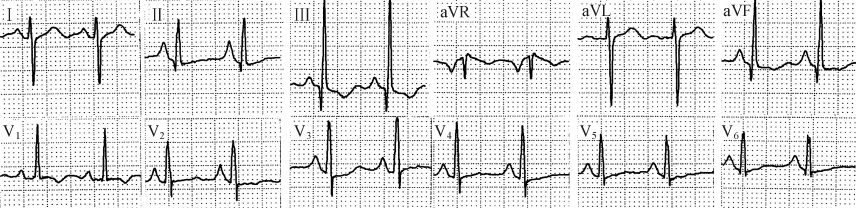
\includegraphics[width=4.71875in,height=4.10417in]{./images/Image00052.jpg}
 \captionsetup{justification=centering}
 \caption{急性腹痛的处理程序}
 \label{fig10-1}
  \end{figure} 

\subparagraph{急性腹痛伴感染性休克}

\hypertarget{text00026.htmlux5cux23CHP1-10-3-2-2-1}{}
(1) 临床表现特点:

①重度中毒表现如寒战,体温迅速升高,精神萎靡,意识障碍等;②休克征象表现为面色苍白,血压下降、尿量减少,脉搏细速,末梢循环不良等;③白细胞明显升高或低于正常甚至核左移。

\hypertarget{text00026.htmlux5cux23CHP1-10-3-2-2-2}{}
(2) 治疗原则:

①扩充血容量,静脉输液;②给予抗生素治疗;③物理方法降温;④寻找感染灶的可能部位并及时处理。

\subparagraph{继发性急性腹膜炎}

继发性急性腹膜炎是指由各种腹腔内病变或外伤所继发的腹膜急性炎症。

\hypertarget{text00026.htmlux5cux23CHP1-10-3-2-3-1}{}
(1) 临床表现特点:

①最突出的症状是腹痛,多为突然发病;常表现为持续性、烧灼样疼痛,随身体的活动而加剧。在炎症最明显处疼痛最重。疼痛范围缩小、程度减轻时,提示炎症局限;反之,则表明炎症扩散。②其他常见症状包括恶心、呕吐、食欲不振、口渴和自觉发热等,发病后患者多表现为尿少和便秘。③急性腹膜炎的特异性体征------腹膜刺激征:肌紧张、压痛和反跳痛。④中毒症状:疾病的早期,患者的体温往往增高并不明显,随着病程的进展,患者体温可以逐渐增高到38℃以上。甚至出现中毒性休克。⑤在空腔脏器穿孔的病例,可出现气腹征------肺肝界叩不清或消失,腹透时隔下有游离气体。⑥腹部穿刺:对诊断非常有帮助。通过对吸出的腹腔液性状进行观察,常可以判断出腹膜炎的病因。

\hypertarget{text00026.htmlux5cux23CHP1-10-3-2-3-2}{}
(2) 治疗原则:

①动态监测患者的病情变化、胃肠减压并留置尿管导尿;②补充血容量、应用抗生素;③积极处理原发病,及时手术处理。

(刘保池 张文武 杨璧卿)

\protect\hypertarget{text00027.html}{}{}

\hypertarget{text00027.htmlux5cux23CHP1-10-4}{}
参 考 文 献

1. 高德明 ,吴金生.现代急腹症学.北京:人民军医出版社,2002

2. Lo Vecchio F,Oster N,Sturmann K,et al. The use of analgesics in
patient with acute abdominal pain. J Emerg Med,1997,15 (6):775

3.
周玲君,刘红香,赵继军.急腹症的早期止痛.中华急诊医学杂志,2006,15(1):91

4. Lo Vecchio F,Oster N,Sturmann K,et al. The use of analgesics in
patient with acute abdominal pain. J Emerg Med,1997,15 (6):775

5. 刘保池 .急腹症的正确诊断与处理.国际外科学杂志,2008,35(6):369

\protect\hypertarget{text00028.html}{}{}

\chapter{恶心与呕吐}

恶心(nausea)、呕吐(vomiting)是临床上常见的症状之一。恶心是一种特殊的主观感觉,表现为胃部不适和胀满感,常为呕吐的前奏,多伴有迷走神经兴奋的症状,如皮肤苍白、流涎、出汗、血压降低及心动过缓等;呕吐是一种胃的反射性强力收缩,通过胃、食管、口腔、膈肌和腹肌等部位的协同作用,能迫使胃内容物由胃、食管经口腔急速排出体外。从某种意义上来说呕吐是机体的一种保护性作用,它可把对机体有害的物质排出体外,但实际上很多呕吐并非摄入有害物质引起,而且频繁和剧烈的呕吐,可引起失水、电解质紊乱和营养障碍。

\subsection{病因与发病机制}

\subsubsection{病因}

引起恶心、呕吐的病因很广泛,包括多方面因素,几乎涉及各个系统。

\subparagraph{感染}

病毒性急性胃肠炎、细菌性急性胃肠炎、急性病毒性肝炎、阑尾炎、胆囊炎、腹膜炎、急性输卵管炎、盆腔炎等。

\subparagraph{腹腔其他脏器疾病}

①脏器疼痛:胰腺炎、胆石症、肾结石、肠缺血、卵巢囊肿蒂扭转。②胃肠道梗阻:幽门梗阻(溃疡病、胃癌、腔外肿物压迫)、十二指肠梗阻(十二指肠癌、胰腺癌)、肠粘连、肠套叠、绞窄疝、克罗恩病、肠结核、肠道肿瘤、肠蛔虫、肠扭转、肠系膜上动脉压迫综合征、输出袢综合征、胃肠动力障碍(糖尿病胃轻瘫、非糖尿病胃轻瘫)、假性肠梗阻(结缔组织病、糖尿病性肠神经病、肿瘤性肠神经病、淀粉样变等)。

\subparagraph{内分泌代谢性疾病}

低钠血症、代谢性酸中毒、营养不良、维生素缺乏症、糖尿病酸中毒、甲状腺功能亢进、甲状腺功能低下、甲状旁腺功能亢进症、垂体功能低下、肾上腺功能低下,各种内分泌危象、尿毒症等。

\subparagraph{神经系统疾病}

中枢神经系统感染(脑炎、脑膜炎)、脑肿瘤、脑供血不足、脑出血、颅脑外伤、脑寄生虫病等。

\subparagraph{药物等理化因素}

麻醉剂、洋地黄类、化疗药物、抗生素、多巴胺受体激动药、非甾体抗炎药、茶碱、酒精、放射线等。

\subparagraph{精神性呕吐}

神经性多食、神经性厌食。

\subparagraph{前庭疾病}

晕动症、梅尼埃病、内耳迷路炎。

\subparagraph{妊娠呕吐}

妊娠剧吐、妊娠期急性脂肪肝。

\subparagraph{其他}

心肺疾患(心肌梗死、肺梗死、高血压、急性肺部感染、肺心病)、泌尿系疾患(急性肾炎、急性肾盂肾炎、尿毒症)、周期性呕吐、术后恶心呕吐、青光眼。

\subsubsection{发病机制}

这是一系列复杂的反射动作,可分为三个阶段,即恶心、干呕与呕吐。恶心发生时,唾液分泌增加,胃蠕动减弱或者消失、排空延缓,十二指肠及近端空肠紧张性增加,出现逆蠕动,导致十二指肠内容物反流至胃内。干呕时胃上部放松而胃窦部短暂收缩;呕吐时胃窦部持续收缩,下食管括约肌松弛,腹肌收缩,膈肌下降,腹压增加,迫使胃内容物急速而猛烈地从胃反流,经食管、口腔而排出体外。呕吐与反食不同,后者系无恶心与呕吐的协调动作而使胃内容物一口一口地反流到口腔。

目前认为的主要的反射通路包括:①信息传入:由自主神经传导(其中迷走神经纤维较交感神经纤维起的作用大)。②呕吐反射中枢:目前认为中枢神经系统的两个区域与呕吐反射密切相关。一是延髓呕吐中枢,另一是化学感受器触发区(chemical
trigger zone,CTZ)。③传出神经:包括迷走神经、交感神经、体神经和脑神经。

通常把内脏末梢传来的冲动引起的呕吐称为反射性呕吐,把CTZ受刺激后引起的呕吐称为中枢性呕吐。延髓呕吐中枢位于延髓外侧网状结构背外侧,迷走神经核附近,主要接受来自消化道和内脏神经、大脑皮质、前庭器官、视神经、痛觉感受器和化学感受区的传入冲动。化学感受器触发区(CTZ)位于第四脑室底部的后极区,为双侧性区域,有密集多巴胺受体。多巴胺受体在CTZ对呕吐介导过程中起重要作用,因为应用阿扑吗啡、左旋多巴、溴隐亭等多巴胺受体激动药可引起呕吐,而其拮抗药、甲氧氯普胺(胃复安)、吗丁啉等药物有止呕作用。化学感受器触发区的5-羟色胺、去甲肾上腺素、神经肽物质和γ-氨基丁酸等神经递质也可能参与呕吐反射过程。CTZ主要接受来自血液循环中的化学、药物等方面的呕吐刺激信号,并发出引起呕吐反应的神经冲动。但CTZ本身不能直接引起呕吐,必须在延髓呕吐中枢完整及其介导下才能引起呕吐,但两者的关系尚不十分明确。CTZ位于血-脑脊液屏障之外,许多药物或代谢紊乱均可作用于CTZ。某些药物如麻醉剂、化学药物、麦角衍生物类药、吐根糖浆等及体内某些多肽物质如甲状腺激素释放激素、P物质、血管紧张素、胃泌素、加压素、血管肠肽等均可作用于CTZ引起恶心呕吐。此外,某些疾病如尿毒症、低氧血症、酮症酸中毒、放射病、晕动症等引起的恶心呕吐也与CTZ有关。

传出神经的呕吐信号传至效应器官,引起恶心呕吐过程,呕吐开始时,幽门关闭,胃内容物不能排到十二指肠,同时,贲门口松弛,贲门部上升,腹肌,膈肌和肋间肌收缩,胃内压及腹内压增高,下食管括约肌松弛,导致胃内容物排出体外。

\subsection{诊断思路}

\subsubsection{病史}

\subparagraph{药物或放射线接触史}

易引起呕吐的常用药物有某些抗生素、洋地黄、茶碱、化疗药物、麻醉剂、酒精等。镭照射线治疗和钴照射线治疗,常引起恶心呕吐。

\subparagraph{其他}

呕吐可为许多系统性疾病的表现之一,包括糖尿病、甲状腺功能亢进症或甲状腺功能减退症、肾上腺功能减退等内分泌疾病、硬皮病等结缔组织病、脑供血不足、脑出血、脑瘤、脑膜炎、脑外伤等中枢神经系统疾病、尿毒症等肾脏疾病。

\subsubsection{临床表现特点}

\subparagraph{呕吐的伴随症状}

呕吐伴发热者,须注意急性感染性疾病;呕吐伴有不洁饮食或同食者集体发病者,应考虑食物或药物中毒;呕吐伴胸痛,常见于急性心肌梗死或急性肺梗死等;呕吐伴有腹痛者,常见于腹腔脏器炎症、梗阻和破裂;腹痛于呕吐后暂时缓解者,提示消化性溃疡、急性胃炎及肠道梗阻性疾病;呕吐伴头痛,除考虑颅内高压的疾患外,还应考虑偏头痛、鼻炎、青光眼及屈光不正等疾病;呕吐伴眩晕,应考虑前庭、迷路疾病、基底椎动脉供血不足、小脑后下动脉供血不足及某些药物(氨基糖苷类抗生素)引起的脑神经损伤。

\subparagraph{呕吐的方式和特征}

喷射性呕吐多见于颅内炎症、水肿出血、占位性病变、脑膜炎症粘连等所致颅内压增高,通常不伴有恶心。此外,青光眼和第Ⅷ对脑神经病变也可出现喷射性呕吐。呕吐不费力,餐后即发生,呕吐物量少,见于精神性呕吐。应注意呕吐物的量、颜色和气味等。呕吐物量大,且含有腐烂食物提示幽门梗阻伴胃潴留、胃轻瘫及小肠上端梗阻等;呕吐物为咖啡样或血性见于上消化道出血,含有未完全消化的食物则提示食管性呕吐(贲门失弛缓症、食管憩室、食管癌等)和见于神经性呕吐、胆囊炎、胆石症及胃大部切除术后等,有时见于妊娠剧烈呕吐、晕动症;呕吐物有酸臭味者,或胃内容物有粪臭味提示小肠低位梗阻、麻痹性肠梗阻、结肠梗阻而回盲瓣关闭不全或胃结肠瘘等。

\subparagraph{呕吐和进食的时相关系}

进食过程或进食后早期发生呕吐,常见于幽门管溃疡或精神性呕吐;进食后期或餐后呕吐,见于幽门梗阻、肠梗阻、胃轻瘫或肠系膜上动脉压迫导致十二指肠雍积;晨起呕吐多见于妊娠呕吐,有时亦见于尿毒症、慢性酒精性中毒和颅内高压等。

\subsubsection{体格检查}

\subparagraph{一般情况}

应注意神志、营养状态、有无脱水、循环衰竭、贫血及发热等。

\subparagraph{腹部体征}

应注意胃型、胃蠕动波、振水声等幽门梗阻表现:肠鸣音亢进、肠型等急性肠梗阻表现:腹肌紧张、压痛、反跳痛等急腹症表现。此外,还应注意有无腹部肿块、疝等。

\subparagraph{其他}

①眼部检查注意眼球震颤、眼压测定、眼底有无视乳头水肿等。②有无病理反射及腹膜刺激征等。

\subsubsection{实验室检查}

主要包括与炎症、内分泌代谢及水盐电解质代谢紊乱等有关的实验室检查。

\subsubsection{其他辅助检查}

可做B超、胃镜、ERCP、超声内镜、CT、磁共振等特殊检查。

\subsection{治疗}

由于引起恶心、呕吐的疾病很多,恶心、呕吐仅是疾病的症状之一。因此,在未明确病因之前不应盲目应用作用于呕吐中枢的强镇吐药物,否则会贻误病情。只有在明确了导致呕吐的病因之后,在积极治疗病因的基础上,才能行必要的对症治疗。

\subparagraph{胃肠道疾病}

包括食管、胃、十二指肠直至空肠、回肠、结肠及直肠在内的任何部位的病变都有可能引起恶心、呕吐的症状,其中以食管狭窄、食管癌、贲门失弛缓、贲门癌、胃窦部嗜酸性肉芽肿、胃窦部巨大溃疡或癌肿、十二指肠溃疡或郁积症、多种原因导致的小肠与大肠梗阻或急性胃、小肠或大肠的炎症性病变为最常见的病因。因消化道良性或恶性病变造成的狭窄或梗阻所致的呕吐,药物治疗是无效的,只有经扩张、置入支架或手术治疗,解除狭窄或梗阻之后,呕吐症状才会消失。对于贲门失弛缓症患者,在未进行扩张或手术治疗之前,可选用钙离子通道拮抗药或硝酸甘油餐前半小时口服或餐前15~30分钟舌下含化治疗,早期可改善呕吐及梗阻症状:或者试用肉毒杆菌毒素行狭窄局部注射治疗。胃肠道急性炎症性病变引起的呕吐,应积极选用抗生素并纠正电解质紊乱及补充维生素;胃肠动力障碍引起的恶心与呕吐则可应用莫沙比利(mosapride,5mg口服,每日3次)、西沙比利(cisapride,5~10mg口服,每日2~4次)、多潘立酮(吗丁啉,10~20mg口服,每日3次;或10mg肌肉注射)、甲氧氯普胺(灭吐灵,胃复安,5~10mg口服;或10~20mg肌肉注射。每日剂量应≤0.5mg/kg,否则易引起锥体外系反应)等促胃肠动力剂;如果呕吐是由胃肠道痉挛所致,则可应用东莨菪碱(0.3mg口服或注射)等抗胆碱能药物。

\subparagraph{肝脏 、胆道及胰腺疾病}

是导致恶心、呕吐的常见病因之一。恶心、呕吐可是急性病毒性肝炎的早期症状,常与食欲减退、厌油腻食物及上腹部饱胀同时出现,随着护肝治疗及适当的休息之后,恶心与呕吐可逐渐消失。呕吐也是胆道梗阻或绞痛常伴随的症状,只有当胆道梗阻或炎症消除之后,呕吐才会停止;急性胰腺炎时常伴随有恶心与呕吐症状,只有随着采用胃肠减压、减少胰液分泌等措施之后,呕吐才会逐步缓解或终止。

\subparagraph{中枢神经系统病变}

包括各种原因所致的脑炎、脑膜炎、脑肿瘤、脑寄生虫病、脑血管病及颅脑外伤等病变,均可引起颅内压力增高而导致恶心、呕吐。治疗的重要措施之一就是应用降低颅内压、减轻脑细胞水肿的药物治疗。脱水治疗后,不仅可改善呕吐的症状,更重要的是起到了保护或恢复脑细胞功能的作用。

\subparagraph{药物所致的呕吐}

多种药物有引起恶心与呕吐的不良反应,一般而言,只要立即停止应用引起呕吐的药物,呕吐症状就会减轻直至消失,因此并不需要应用镇吐类药物。目前临床上对某些恶性肿瘤或血液系统的恶性疾病(如白血病、恶性淋巴瘤、多发性骨髓瘤、恶性组织细胞病等)采用联合化疗或放疗,或对某些恶性肿瘤采用抗癌药物行介入治疗。但无论在治疗过程中或治疗之后,均可引起较为严重的胃肠道不良反应,最突出的表现就是恶心与呕吐。为了预防或减轻此不良反应,常可应用镇吐药物进行治疗,常用的药物有昂丹司琼(ondansetron,奥丹西龙,商品名:枢复宁。常用8mg口服或静脉注射)、格拉司琼(granisetron,商品名:康泉。成人剂量每次40μg/kg,或标准剂量3mg,静脉滴注)等。必须指出,应用这些作用强的镇吐药物之后,也会产生中枢神经系统、心血管系统或胃肠道的不良反应,故应严格控制药物剂量及间隔时间。

\subparagraph{神经 、精神因素所致的呕吐}

对此类原因所致的呕吐,心理治疗是关键。首先应消除患者的精神心理障碍,其次可配合药物治疗,常用的药物是镇静药与胃肠促动力剂、重者可采用多塞平或氟西汀等抗抑郁药物治疗。禁忌应用昂丹司琼(奥丹西龙)等强烈作用的镇吐药。

\protect\hypertarget{text00029.html}{}{}

\hypertarget{text00029.htmlux5cux23CHP1-11-4}{}
参 考 文 献

1. 陈文彬,潘祥林.诊断学.第7版.北京:人民卫生出版社,2008

2. 陈新谦,金有豫,汤光.新编药物学.第17版.北京:人民卫生出版社,2011

\protect\hypertarget{text00030.html}{}{}

\chapter{急 性 腹 泻}

正常人一般每日排成形大便1次,粪便平均重量为150~200g,一般不超过200g,其中水分占60\%~70\%,约150ml左右。少数人每天排便2~3次或2~3天才排1次,但若粪质成形,性状与常人无异,亦属正常。

腹泻(diarrhea)是指排便习惯和粪便性状发生变化,排便次数增多(每天3次以上),粪质稀薄,水分增加(水分超过85\%),粪便量增加(超过200g/d)。便质不成形、稀溏或呈液状,有时含有脓血或带有未消化食物及脂肪。确定是否有腹泻应根据个体的大便习惯而异。

腹泻可根据病程分为急性腹泻和慢性腹泻两种,也可依病因分为感染性腹泻和非感染性腹泻两大类。急性腹泻是指起病急骤、病程较短,病程在2~3周之内,极少超过6~8周。慢性腹泻指病程至少在4周以上,常超过6~8周,或间歇期在2~4周内的复发性腹泻。腹泻常伴有排便紧迫感、肛门不适或大便失禁。腹泻可导致水电解质丢失,严重时可引起大量失水,导致低血容量性休克和急性器官功能衰竭,甚至因电解质严重紊乱引起严重心律失常而死亡。

\subsection{病因与发病机制}

在禁食期间,正常人肠腔内液体含量很少。但正常三餐摄取后,每天约有9L液体进入肠道,其中2L来自进食的食物和饮料,其余来自消化道分泌液,包括唾液1.5L、胃液2.5L、胰液1.5L、胆汁0.5L和小肠液1.0L。进入胃肠道的食糜在通过小肠时,食糜的渗透度变得与血浆相同,其中90\%的水分被其吸收。食糜在到达回肠末端时,已呈等渗状态,每天仅有1~2L的液体进入结肠,而结肠也具有强大的吸收水分的功能,使大便最终含水量只有100~200ml。若胃肠道的分泌、消化、吸收和运动等功能障碍,使消化道分泌的液量增加,食物不能完全分解,吸收量减少和肠胃蠕动加速等,最终可导致粪便性状稀薄、次数增加而形成腹泻。腹泻的发病机制相当复杂,从病理生理角度分为四类,部分腹泻的发病可有几个因素并存,具体如下:

\subparagraph{分泌性腹泻}

肠道液体主要由黏膜隐窝细胞分泌,大部分经肠绒毛腔面上皮细胞吸收。当各种刺激因子刺激肠黏膜细胞分泌的量超过其吸收能力时,所引起的腹泻称分泌性腹泻(secretory
diarrhea)。刺激肠黏膜分泌的因子可分为四类:①细菌的肠毒素,如霍乱弧菌、大肠埃希菌、沙门菌等毒素;②神经体液因子,如血管活性肠肽(VIP)、血清素、降钙素等;③免疫炎性介质,如前列腺素、白三烯、血小板活化因子、肿瘤坏死因子、白介素等;④去污剂,如胆盐和长链脂肪酸,通过刺激阴离子分泌和增加黏膜上皮通透性而引起分泌性腹泻;⑤各种通便药,如蓖麻油、酚酞、芦荟、番泻叶等均可引起分泌性腹泻。

肠道分泌电解质和水分的机制相当复杂。近年发现,肠黏膜隐窝细胞中的第二信使如环磷酸腺苷(cAMP)、环磷酸鸟苷(cGMP)、钙离子等的增加是诱导黏膜隐窝细胞分泌的重要环节。霍乱弧菌和致病性大肠埃希菌的毒素首先与上皮细胞刷状缘上的受体结合,激活腺苷环化酶-cAMP系统,致cAMP浓度增高,引起大量肠液分泌;艰难梭菌(C.difficile)是通过钙离子增加而引起分泌性腹泻;血管活性肽瘤(VIP瘤)引起的腹泻是一种非感染性的分泌性腹泻,肿瘤释出的VIP能激活肠黏膜的腺苷酸环化酶,刺激小肠大量分泌液体,故而出现霍乱样的严重水泻,称为胰性霍乱,常伴有严重的低钾血症和代谢性酸中毒;胃泌素瘤能分泌大量的胃泌素,刺激壁细胞分泌大量胃液,过多胃液进入小肠后,不仅可损害空肠黏膜,而且促进肠道蠕动,使胰脂肪酶灭活,脂肪消化障碍而更加重腹泻。分泌性腹泻还可见于直肠分泌性绒毛状腺瘤、肠淋巴瘤、炎症性肠病、肠肉芽肿性疾病、结缔组织病、恶性类癌综合征、甲状腺髓样癌等。

分泌性腹泻的特点是:①禁食不减轻腹泻;②肠液与血浆的渗透压相同;③大便呈水样,量多,无脓血;④一般不伴有腹痛;⑤肠黏膜组织学基本正常。

\subparagraph{渗透性腹泻}

由于肠腔内含有大量不能被吸收的溶质,导致肠腔内渗透压升高,大量液体被动进入肠腔而引起腹泻,称为渗透性腹泻(osmotic
diarrhea)或吸收不良性腹泻(malabsorption diarrhea)。见于:

\hypertarget{text00030.htmlux5cux23CHP1-12-1-2-1}{}
(1) 高渗性药物:

口服镁盐、乳果糖、甘露醇或山梨醇等高渗性药物。

\hypertarget{text00030.htmlux5cux23CHP1-12-1-2-2}{}
(2) 高渗性食物:

主要是某些碳水化合物,由于水解酶缺乏或其他原因而导致食物吸收不良,形成高渗透压性的肠内容物而引起腹泻。临床上最常见的是原发性乳糖酶缺乏,患者口服牛奶或奶制品后即可引起腹泻。

\hypertarget{text00030.htmlux5cux23CHP1-12-1-2-3}{}
(3) 消化不良:

胃大部分切除术后、萎缩性胃炎和胃癌患者的胃液分泌减少,慢性胰腺炎、胰腺切除术后使胰液分泌减少,严重肝病或胆管梗阻可导致胆汁分泌或排泄减少,使食物不能充分被消化,营养物质不能被吸收,致使高渗性肠内容物增多而造成腹泻。

\hypertarget{text00030.htmlux5cux23CHP1-12-1-2-4}{}
(4) 吸收不良:

①黏膜透过性异常:由于小肠黏膜细胞的特殊病变如绒毛或微绒毛的变形、萎缩等变化,导致小肠的有效吸收面积缩小和黏膜透过水和电解质减少而导致腹泻。见于小儿乳糜泻、热带和亚热带斯泼卢等疾病。②肠吸收面积减少:如小肠切除后等。③肠黏膜充血、水肿:由于门静脉内压力增加,引起肠道黏膜广泛充血与水肿,影响肠道内营养物质的吸收而发生腹泻。④细菌繁殖过多:在某些疾病状态下,如肝硬化、小肠浸润性疾病引起的部分性肠梗阻或某些小肠失蠕动(如系统性硬皮病)、盲袢等,小肠内细菌可以过多繁殖。由于细菌分泌的毒素可影响消化酶的作用,以及细菌分解物结合胆盐,使其失去形成微胶粒的能力,导致脂肪等食物的消化和吸收受到障碍等,可引起腹泻或脂泻。⑤吸收抑制:如先天性氯泻(congenital
chloriderrhea),是由于氯的主动吸收功能不全而钠的吸收过程正常,以致肠内容物中由于氢和氯化物增加,但缺乏碳酸氢钠与之中和而使肠液呈酸性,回肠和结肠内液体积聚而引起腹泻。氯泻也可继发于长期腹泻而缺钾的患者。

渗透性腹泻的特点是:①当引起腹泻的原因除去(如禁食)之后,腹泻即可停止或减轻;②肠腔内的渗透压可超过血浆渗透压;③粪中含有大量未被完全吸收或消化的食物。

\subparagraph{肠动力紊乱(motility disturbances)}

许多药物、疾病和胃肠道手术可改变肠道的正常运动功能,促使肠蠕动加速,以致肠内容物过快通过肠腔,因影响消化与吸收而发生腹泻。肠动力过缓亦可导致腹泻,其原因为结肠型的细菌在小肠定植和过度生长,从而使脂肪、胆盐和碳水化合物的吸收受到影响。此类腹泻可见于淀粉样变性、硬皮病、糖尿病性神经病变、胃大部切除术后、幽门或肛门括约肌切除术后、肠易激综合征、情绪性腹泻、毒性甲状腺肿病、恶性类癌综合征等。

此种腹泻的特点是粪便稀烂或水样,肠鸣音亢进,常伴有腹痛,但大便中很少有炎症细胞。

\subparagraph{渗出性腹泻(exudative diarrhea)}

又称炎症性腹泻(inflammatory
diarrhea)。肠黏膜炎症时渗出大量黏液、脓、血,可致腹泻。此类腹泻可见于:①炎症性肠病,如克罗恩病和溃疡性结肠炎;②感染性炎症:来自侵入性病原体及其毒素,如志贺痢疾杆菌、沙门菌属、弯曲杆菌、耶尔森菌(Yersinia)、结核杆菌、阿米巴原虫、艰难梭菌等的感染;③缺血性炎症;④肠放射损伤;⑤嗜酸性肠炎:为嗜酸性粒细胞浸润胃肠道全层,可累及全胃肠道或节段性,表现为脂肪泻、腹痛、恶心、呕吐、消瘦,外周血嗜酸性粒细胞可增多。

渗出性腹泻的特点是:①粪便松散或水样,含有黏液和脓血,左侧结肠病变所致者常带有肉眼可见的脓血便,小肠病变一般无肉眼可见的脓血便。②腹泻和全身症状、体征的严重程度因肠受损程度而异。

需要指出和值得注意的是,同一种疾病产生的腹泻常常有多种机制参与,且腹泻的病因并不单纯,可同时或先后有几个病因并存。临床上最常见的为各种肠道感染、炎症、结肠和直肠癌、葡萄球菌肠毒素所引起的食物中毒及肠道易激综合征等。

\subsection{诊断思路}

腹泻的病因诊断要依靠病史、症状、体征,并结合辅助检查,尤其是粪便检验的结果,综合分析后得出结论。对一时难以明确诊断者,可进一步作X线钡剂检查和(或)结肠镜检查;对胆、胰疾病可选用超声、CT、MR、逆行胰胆管造影(ERCP)等影像学诊断方法加以明确诊断;对小肠吸收不良者可行小肠吸收功能试验、呼气试验、小肠黏膜活检等以明确诊断。但在诊断过程中应注意以下几点。

\subsubsection{病史}

\subparagraph{年龄与性别}

婴幼儿起病的腹泻,应考虑先天性小肠消化吸收障碍性疾病,如双糖酶缺乏症、先天性氯泻等。病毒性胃肠炎和大肠埃希菌性肠炎多见于婴幼儿;细菌性痢疾以儿童和青壮年多见;结肠癌多见于中年或老年;阿米巴痢疾则以成年男性居多;功能性腹泻、甲亢和滥用泻剂者多见于女性,而结肠憩室与结肠癌则多见于男性。

\subparagraph{起病与病程}

需询问国际、国内和郊区旅游史、近期服用了哪些药物或免疫抑制剂、是否亲密接触动物等。急性腹泻均应注意询问接触或摄入不洁食物史、起病与演变过程等。急性食物中毒性感染常于进食后2~24小时内发病;手术后发病,尤其是长期接受抗生素治疗者,应考虑金黄色葡萄球菌肠炎、难辨梭状芽胞杆菌性肠炎等。由功能性腹泻、血吸虫病、溃疡性结肠炎、克罗恩病等所引起的腹泻,可长达数年或数十年。功能性腹泻、吸收不良综合征和结肠憩室炎所致的腹泻,常呈间歇性的发作。

\subparagraph{排便与粪便性状}

往往可以提示病变部位或性质。腹泻量多、水样、色淡、多泡沫、恶臭、无脓血、无里急后重,提示病变位于小肠;黏液带果酱色血便,病变多在上段结肠;粉红色脓血便,病变多在下端结肠;粪便表面带血或伴明显里急后重,病变多在直肠。急性腹泻先为水样后为脓血便,一日多至数十次,伴有里急后重者急性细菌性痢疾的可能性较大;粪便暗红色、酱色状或血水样,提示阿米巴痢疾可能;粪便稀水样,无里急后重,多为食物中毒性感染;若在进食后6~24小时发病则以沙门菌属、变形杆菌、产气荚膜梭状芽胞杆菌感染的可能性大;若在进食后2~5小时发病,伴有剧烈呕吐者可能为金黄色葡萄球菌感染所致。呕吐物和腹泻均呈米泔水样,失水严重,应考虑霍乱;若粪便带有恶臭,呈紫色血便,应考虑急性出血性坏死性肠炎。吸收不良综合征时粪便有食物残渣、未消化或发酵物,可奇臭;结肠炎症引起的腹泻粪便带脓血;肠结核和肠易激综合征常有腹泻与便秘交替现象。肠易激综合征的功能性腹泻多在清晨起床后和早餐后发生,每日2~3次,粪便有时含大量黏液。影响睡眠的夜间腹泻多系器质性疾病所致。

\subparagraph{腹泻与腹痛}

腹泻伴有里急后重且下腹或左下腹持续性腹痛,腹痛于便后可稍减轻,提示病变位于直肠或乙状结肠;腹泻无里急后重,伴脐周腹痛为小肠性腹泻。

\subparagraph{伴随症状}

急性腹泻伴有高热,以细菌性痢疾、沙门菌属食物中毒感染居多;有里急后重以细菌性痢疾、阿米巴痢疾、急性血吸虫病可能性大,而食物中毒性感染大多无里急后重。

\subsubsection{体格检查}

对腹泻患者应做全面仔细的体格检查。如腹部检查被触及包块,常提示肿瘤或炎症性疾病;若包块位于左下腹,应疑及左侧结肠癌、乙状结肠憩室炎,或癌肿造成的肠腔狭窄使粪块壅积于梗阻的近端肠腔,或为单纯的粪块堆积;若位于右下腹,应想到右侧结肠癌、肠结核、克罗恩病等。如腹部压痛明显,可见于克罗恩病、结肠憩室炎、盆腔或阑尾脓肿。肛门指检应列为常规检查,若触及坚硬、结节状、固定的肿块,指套上有血迹常提示直肠癌。

\subsubsection{辅助检查}

大多数腹泻都是自限性的,因此辅助检查价值有限。但对病程较长和对保守治疗无效的患者须选择相应的辅助检查,以明确病因诊断。

\subparagraph{粪便检查}

粪便应为现场留取,或是短时间内留在标本盒中的新鲜标本。应注意粪便的形态、量、黏稠度及有无食物残渣、黏液、血和脓性分泌物等。大便常规检验、隐血实验,粪便涂片查脓细胞、寄生虫及虫卵、脂肪、未消化食物等,大便致病菌培养等,对分泌性腹泻测定粪便的电解质和渗透压等,对腹泻的定位和定性诊断非常重要。粪便镜检出现白细胞往往提示肠道细菌感染,当粪便中的白细胞计数>
15/HP,同时伴有红细胞时,临床可诊断为痢疾;而动力试验检查可以发现弧菌感染,这是诊断霍乱最简单的方法。

\subparagraph{胃肠内镜检查}

对腹泻病因、部位不明者可酌情进行胃镜、乙状结肠镜、结肠镜或小肠镜检查,必要时重复同一检查或同一患者行不同的内镜检查。根据在直视下病变的性质、范围、严重程度以及活检的病理结果,明确腹泻的病因诊断,尤其对胃肠炎症性疾病、肿瘤等的诊断和鉴别诊断具有肯定价值。

\subparagraph{影像学检查}

腹部平片可显示胰腺钙化及钙化性结石;胃肠钡餐检查可以观察胃肠道的运动功能状态,发现器质性病变,对结肠癌、炎症性肠病具有较高诊断价值;腹部B超是了解有无肝胆胰疾病的最常用方法;腹部CT
或MRI对诊断肝、胆、胰等内脏疾病有肯定价值。

\subparagraph{小肠功能检查}

可行小肠吸收功能试验、呼气试验、小肠黏膜活检以检查小肠吸收不良。

\subsection{处理原则}

腹泻是症状,针对病因是根本性治疗,在未明确病因前,根据腹泻的病理生理特点给予对症和支持治疗也很重要,但必须谨慎使用止泻和止痛药物,以免造成误诊和漏诊。

\subsubsection{病因治疗}

\subparagraph{抗病原体治疗}

经验性的抗生素治疗并不适用于所有急性腹泻患者,这是由于:①大多数急性腹泻患者凭借自身的抵抗力足以有效清除病原,研究发现50\%的感染性腹泻患者,不使用抗生素也可以在3天内恢复;②应用抗生素后反而会引起药物的不良反应,如难辨梭状芽胞杆菌感染和细菌耐药;③应用抗生素可延长病原菌的毒素排出时间等。而下列急性腹泻患者推荐经验性地使用抗菌药物:①有明确细菌感染征象者,如发热伴粪便镜检中有白细胞者;②临床诊断的痢疾(粪便镜检白细胞>
15/HP,同时出现红细胞)患者;③危及生命的感染,如霍乱;④旅行者腹泻,这些患者往往需要较短的时间内迅速缓解症状;⑤免疫缺陷或免疫低下者。

抗感染治疗以针对病原体的抗菌治疗最为理想,如复方新诺明、环丙沙星、诺氟沙星、左旋氧氟沙星、加替沙星等喹诺酮类适用于志贺菌属、沙门菌、弯曲杆菌、大肠埃希菌等所致的腹泻;甲硝唑或万古霉素适用于难辨梭状芽胞杆菌感染引起的假膜性肠炎;肠结核应用如利福平、异烟肼、乙胺丁醇、吡嗪酰胺、对氨基水杨酸、链霉素等抗结核药物中的三种或四种联合治疗;阿米巴痢疾可选用甲硝唑。病毒性腹泻常不用抗生素,可使用盐酸小檗碱(黄连素)。大肠埃希菌O\textsubscript{157}
∶H\textsubscript{7}
感染亦不用,因现有抗生素治疗并无疗效,且增加溶血-尿毒综合征的发生。一般在送检大便培养后,可经验性地予以氟喹诺酮类抗生素,若临床提示弯曲杆菌者应加用红霉素、罗红霉素等大环内酯类抗生素。

\subparagraph{其他}

主要是针对发病机制治疗,如对乳糖不耐受症者不宜用乳制品或应剔除食物中的乳糖成分,而成人乳糜泻患者则需禁食麦制品(包括大麦、小麦、燕麦和裸麦)或剔除食物中的麦胶类成分。分泌性腹泻需同时补充葡萄糖以保证热量的吸收。慢性胰腺炎应补充多种消化酶。因服药所致的药源性腹泻应及时停用有关药物,高渗性腹泻应停用或停食引起高渗的药物和食物。消化道肿瘤可手术切除或化疗以治疗原发病。生长抑素类似物奥曲肽可抑制肿瘤分泌激素,可用于类癌综合征及神经内分泌肿瘤引起的腹泻。炎症性肠病可选用柳氮磺胺吡啶或5-氨基水杨酸制剂,如美沙拉嗪(颇得斯安)等。空肠广泛性黏膜病变和空肠切除后所致腹泻,乃因胆盐未能在小肠被重吸收而进入结肠,并在此被结肠内的细菌脱结合为游离胆酸,后者刺激结肠引起腹泻,服用考来烯胺或消胆胺可将胆汁酸吸附而终止腹泻。胆盐缺乏性的腹泻,可用中链脂肪酸补充脂肪类物质,因中链脂肪酸可不经胆盐水解而被吸收。短肠综合征者最好用多聚体形式的葡萄糖。

\subsubsection{对症支持疗法}

\subparagraph{饮食治疗}

急性腹泻时的饮食应以易消化、易吸收的流质或半流质为宜,避免牛奶和乳制品食物。

\subparagraph{纠正腹泻所引起的水 、电解质与酸碱平衡紊乱}

腹泻有时可引起不同程度的脱水,轻症者可用口服补液,严重腹泻伴失水者应立即静脉补液。应根据脱水的性质和血清电解质情况补充氯化钠、氯化钾等;若伴有酸碱平衡紊乱,也应及时纠正。一般来说,由于肠液电解质几乎与血浆浓度相仿且偏碱性,故水与电解质的补充大部分应以碳酸氢钠-生理盐水或林格液较适宜。

\subparagraph{纠正营养失衡}

对腹泻引起营养缺乏者,应根据病情相应地补充各种水溶性和(或)脂溶性维生素、葡萄糖、氨基酸、脂肪乳、白蛋白、丙种球蛋白等营养物质。若伴有缺铁、缺钙、缺镁等者亦应及时补充。必要时可予输注血浆、全血等。锌缺乏易致腹泻是和锌参与肠道水和电解质的转运、小肠渗透性、肠细胞酶的功能,增强肠道组织的修复,增强局部免疫,以控制细菌过度生长和与早期病原菌清除等有关。故在急性腹泻时补锌可缩短病程,减轻症状,如大便次数和粪便排出量的减少,使未来2~3个月中腹泻发病率下降。

\subparagraph{胃肠黏膜保护剂}

硫糖铝、枸橼酸铋钾、米索前列醇、双八面体蒙脱石(思密达)等有胃肠黏膜保护作用,硫糖铝和枸橼酸铋钾可黏附覆盖在溃疡面上阻止胃酸和胃蛋白酶继续侵袭溃疡面、促进内源性前列腺素的合成和刺激表皮生长因子分泌;但为避免铋在体内蓄积,枸橼酸铋钾不宜连续长期服用。米索前列醇具有抑制胃酸分泌、增加胃十二指肠黏膜黏液/碳酸氢钠盐分泌和增加黏膜血流的作用,但可引起子宫收缩和腹泻,孕妇忌服。蒙脱石散可用于感染性或非感染性腹泻,可口服亦可灌肠。

\subparagraph{微生态制剂}

常用双歧杆菌嗜酸乳杆菌肠球菌三联活菌(金双歧,培菲康,每次420~630mg,每日2~3次餐后服用)、嗜酸乳杆菌(乐托尔,每次2粒口服,每日2次,首剂加倍)、双歧杆菌(丽珠肠乐,每次0.35~0.7g,每日2次)、复合乳酸菌(聚克,每次1~2粒,每日1~3次)、地衣芽胞杆菌活菌(整肠生,每次0.5g,每日3次)、乳酶生(表飞鸣,每次0.3~1.0g,每日3次餐前服用)等以调节肠道菌群。它可以减少抗生素的应用,对旅行者腹泻、抗生素相关性腹泻、儿童腹泻和难辨梭状芽胞杆菌引起的腹泻有较好疗效。

\subparagraph{止泻药}

排便太频或失水、电解质过多,或引起痛苦时宜用止泻剂,使用止泻剂应注意以下原则:①严格掌握指征,主要针对严重失水者、非感染性腹泻者,并不是对所有腹泻均须使用止泻药,以免影响腹泻时将胃肠的有害物质排出体外的保护作用。当有病因治疗时,对轻度腹泻者多不必止泻,不一定加以抑制腹泻。②因止泻药可引起肠动力障碍,使致病菌定植和侵袭,延长排泄时间,故对诊断不明又不能排除感染时需慎用,明确感染性腹泻者禁用。③局限于直肠、乙状结肠的溃疡性结肠炎患者的腹泻主要是由于炎症激惹、刺激,而全胃肠通过时间并不缩短,应予抗炎治疗。④诊断不明又未能排除严重疾病时,用止泻剂应慎重,不能因症状控制而放松诊断性检查。⑤尽量避免或仅短期服用可引起药瘾性的药物(如复方樟脑酊、可待因等)。常用止泻剂有:

\hypertarget{text00030.htmlux5cux23CHP1-12-3-2-6-1}{}
(1) 地芬诺酯(苯乙哌啶,diphenoxylate,止泻宁):

为哌替啶(度冷丁)的衍生物。能减少肠蠕动,并有收敛作用,可用于各种因胃肠运动增快引起的腹泻。临床上常用复方地芬诺酯(每片含地芬诺酯2.5mg,阿托品0.025mg),每次口服1~2片,每日2~4次。大剂量时可产生欣快感,长期服用会成癮,产生依赖性。肝、肾功能损害,尤其是严重肝病时,可诱发肝性脑病;重症溃疡性结肠炎时,因抑制肠蠕动,可诱发中毒性结肠扩张。儿童患者慎用。

\hypertarget{text00030.htmlux5cux23CHP1-12-3-2-6-2}{}
(2) 洛哌丁胺(苯丁哌胺,loperamide;易蒙停,imodium):

其化学结构与地芬诺酯相似。可抑制平滑肌收缩,抑制肠蠕动。其作用强度比吗啡、阿托品大。口服后易吸收,4~6小时达高峰,分布于肝、肾,并从尿、粪排出。应用指征同地芬诺酯。其作用还有:①阻断钙通道,抑制肠运动;②抑制分泌;③抑制调钙蛋白,增加Na\textsuperscript{+}
、Cl\textsuperscript{−}
吸收。比地芬诺酯作用强,用药后迅速止泻。每次2mg口服,每天2~3次。

\hypertarget{text00030.htmlux5cux23CHP1-12-3-2-6-3}{}
(3) 可乐定(氯压定,clonidine):

为α\textsubscript{2}
肾上腺素能药物,可刺激肠细胞上特异的节后α\textsubscript{2}
受体,促进Na\textsuperscript{+} 和Cl\textsuperscript{−}
的吸收,抑制HCO\textsubscript{3} \textsuperscript{−}
和Cl\textsuperscript{−}
的分泌,为强力的止泻剂,因其中枢性低血压和镇静作用限制了它的应用。但糖尿病患者合并严重的自主神经病变时,并不出现低血压,而仅有止泻作用,可用于糖尿病性腹泻。

\hypertarget{text00030.htmlux5cux23CHP1-12-3-2-6-4}{}
(4) 奥曲肽(善得定,sandostatin):

是生长抑素(somatostatin,STT)的人工合成类似物,可有效治疗胃肠激素失常性腹泻(如VIP瘤、胃泌素瘤、生长抑素瘤和类癌综合征等所致的腹泻),常用剂量为0.3~0.75mg/d,分3次皮下注射。

\hypertarget{text00030.htmlux5cux23CHP1-12-3-2-6-5}{}
(5) 吲哚美辛(消炎痛,indomethacin):

能抑制胰性霍乱、甲状腺癌以及小肠绒毛腺癌的分泌性腹泻。主要是吲哚美辛可降低前列腺素E\textsubscript{2}
(PGE\textsubscript{2}
)水平而达到止泻效果,而对炎症性肠病,吲哚美辛无止泻作用。

\hypertarget{text00030.htmlux5cux23CHP1-12-3-2-6-6}{}
(6) 钙拮抗剂:

硝苯地平、维拉帕米等,对分泌性腹泻有效。

\hypertarget{text00030.htmlux5cux23CHP1-12-3-2-6-7}{}
(7) 收敛吸附剂:

如鞣酸蛋白(tannalbin,每次1~2g,每日3次)、碱式碳酸铋(次碳酸铋,每次0.3~0.9g,每日3次餐前服用)、药用炭(每次1.5~4g,每日2~3次餐前服用)等,可选择性用于炎症性腹泻。

\hypertarget{text00030.htmlux5cux23CHP1-12-3-2-6-8}{}
(8) 鸦片制剂:

如复方樟脑酊,能增强肠平滑肌张力,减低胃肠推进性蠕动,使粪便干燥而止泻。腹泻早期或腹胀者不宜使用。多用于较严重的非细菌感染性腹泻。2~5ml/次,每天3次。

\hypertarget{text00030.htmlux5cux23CHP1-12-3-2-6-9}{}
(9) 双八面体蒙脱石(思密达):

是一种高效消化道黏膜保护剂,主要通过保护肠黏膜屏障功能达到抗腹泻作用。其作用机制是:蒙脱石散对消化道内的病毒、病菌及其产生的毒素有极强的选择性固定、抑制作用;对消化道黏膜有很强的覆盖能力,并通过与黏液糖蛋白相互结合,修复、提高黏膜屏障的防御功能。它不进入血液循环系统,6小时左右连同所固定的攻击因子随消化道自身蠕动排出体外。蒙脱石散不影响X线检查,不改变大便颜色,常用剂量下不改变肠道生理运转时间,也不影响其他药物的生物利用度。基本无副作用,极少数患者产生轻度便秘,减量后可继续服用。用法:成人每次1袋(3g/袋)冲服,每日3次;2岁以上儿童每日2~3次,每次1袋;1~2岁幼儿每日1~2次,每次1袋;1岁以下幼儿每日1袋,分2次服用。治疗急性腹泻时首剂量应加倍。

\hypertarget{text00030.htmlux5cux23CHP1-12-3-2-6-10}{}
(10) 抗胆碱药:

适用于功能性及痉挛性腹痛者,可与镇静药合用。

\subparagraph{止痛剂}

对伴有明显腹痛的患者应使用止痛剂治疗。654-2、阿托品、丙胺太林等具有解痉、止痛作用,但青光眼、前列腺肥大者慎用,严重炎症性肠病患者中可诱发巨结肠,亦应慎用。胃肠道选择性钙拮抗剂匹维溴铵、西托溴铵等副作用较少。抗焦虑药有时也可缓解症状。

\protect\hypertarget{text00031.html}{}{}

\hypertarget{text00031.htmlux5cux23CHP1-12-4}{}
参 考 文 献

1. Longstreth GF,Thompson WG,Chey WD,et al. Functional bowel
disorders. Gastroenterology,2006,130(5):1480

2. Delvaux M,Gay G. Management of a patient with functional diarrhea.
Gastroenterol Clin Biol,2006,30(3):415

3. Beattie RM,Croft NM,Fell JM,et al. Inflammatory bowel disease.
Arch Dis Child,2006,91(5):426

4. 沈晓明 ,王卫平.儿科学.第7版.北京:人民卫生出版社,2008:255

5.
陈新谦,金有豫,汤光.新编药物学.第17版.北京:人民卫生出版社,2011:496

\protect\hypertarget{text00032.html}{}{}

\chapter{消化道出血}

消化道以屈氏(Treitz)韧带为界,其上的消化道出血称为上消化道出血(upper
gastrointestinal
hemorrhage,UGIH),其下的消化道出血为下消化道出血(lower
gastrointestinal
hemorrhage,LGIH)。消化道急性大量出血,临床表现为呕血、黑粪、血便等,并伴有血容量减少引起的急性周围循环衰竭,是消化系病常见的急症。病情危重者,可危及生命。

\section{上消化道出血}

上消化道出血(UGIH)是指Treitz韧带以上的消化道,包括食管、胃、十二指肠或胰胆等病变引起的出血,胃空肠吻合术后的空肠病变出血亦属这一范围。上消化道大出血一般指在数小时内失血量超过1000ml或循环血量的20\%;一次出血量500ml以上,出现直立性头晕,心率>
120次/分,血压<
90mmHg,或比原来基础压低25\%以上;1~2天内血红蛋白(Hb)<
70g/L(7.0g/dl),红细胞计数(RBC)< 3 × 10\textsuperscript{12}
/L(300万/mm\textsuperscript{3} ),血细胞比容<
0.25(25\%);24小时内需输血约2000ml以上。其临床表现主要是呕血和(或)黑粪,常伴有血容量减少引起的急性周围循环衰竭。

为便于诊治和评判预后,目前临床上常依病因不同将UGIB分为以下两大类:

\subparagraph{非静脉曲张性上消化道出血(nonvariceal upper gastrointestinal}
bleeding,NVUGIB)

是指Treitz韧带以上的消化道的非静脉曲张性疾患引起的出血,包括胰管或胆管的出血和胃空肠吻合术后吻合口附近疾患引起的出血。NVUGIB的病因繁多,多为上消化道病变所致,少数为胆胰疾患引起,其中以消化性溃疡、急性糜烂出血性胃炎、上消化道肿瘤、急慢性上消化道黏膜炎症最为常见。少见的有食管贲门黏膜撕裂综合征、上消化道血管畸形、Dieulafoy溃疡、食管裂孔疝、胃黏膜脱垂或套叠、急性胃扩张或扭转、理化和放射损伤、壶腹周围肿瘤、胰腺肿瘤、胆管结石、胆管肿瘤等。某些全身性疾病,如感染、肝肾功能障碍、凝血机制障碍、结缔组织病等也可引起本病。年发病率为(50~150)/10万,病死率为6\%~10\%。

\subparagraph{食管胃静脉曲张出血(esophageal and gastric variceal bleeding,EGVB)}

是指由于肝硬化等病变引起的门静脉高压,致使食管和(或)胃壁静脉曲张,在压力升高或静脉壁发生损伤时,曲张静脉发生破裂出血,临床上主要表现为呕血、黑便、便血和周围循环衰竭征象。其特征是起病突然,出血量大且易反复,病情凶险,病死率高。EGVB的病因可见于所有引起门静脉高压的疾病,在我国以肝硬化最为常见。

\subsection{病因与发病机制}

上消化道出血的病因很多,大多是上消化道本身病变(溃疡、炎症、肿瘤)所致,少数是全身疾病的局部表现(如各类紫癜、白血病、再障等)。但临床上最常见的病因是消化性溃疡、食管胃底静脉曲张破裂、急性糜烂出血性胃炎和胃癌,这些病因占UGIH的80\%~90\%。常见上消化道出血的病因及其发生机制如下:

\subsubsection{消化性溃疡}

消化性溃疡(peptic
ulcer,PU)主要指发生在胃和十二指肠的慢性溃疡,即胃溃疡(gastric
ulcer,GU)和十二指肠溃疡(duodenal
ulcer,DU),因溃疡形成与胃酸/胃蛋白酶的消化作用有关而得名。胃、十二指肠溃疡出血是消化性溃疡最常见的并发症,也是上消化道出血的最常见的病因,占40\%~50\%,其中尤其以十二指肠球部溃疡居多(十二指肠溃疡占30\%~40\%,胃溃疡占10\%~15\%)。出血是消化性溃疡活动的表现,可因溃疡周围小血管充血、破裂,或因溃疡基底肉芽组织的血管壁被侵蚀而导致破裂出血,大多数为动脉出血。在瘢痕组织形成中的血管硬化,失去了弹性,如发生破裂则不易止血。致命性大出血多属十二指肠球后溃疡或胃小弯穿透性溃疡侵蚀较大血管所致。胃溃疡出血多发部位是胃小弯附近,出血来源常是胃左、胃右动脉及其分支;十二指肠溃疡出血多发部位是十二指肠球部后壁与球后溃疡,出血多来源于胃十二指肠或胰十二指肠上动脉及其分支。十二指肠前壁附近无大血管,故此处的溃疡常无大出血。部分病例可有典型的周期性、节律性上腹疼痛,出血前数日可出现溃疡疼痛加重及疼痛规律的改变;出血后疼痛减轻或缓解,这是血液中和胃酸或血凝块覆盖在溃疡面上减少了胃酸、胃蛋白酶的侵蚀作用,使疼痛缓解。但约有10\%~15\%患者可无溃疡病史而以上消化道出血为首发症状。胃镜检查是确诊消化性溃疡首选的检查方法。

\subsubsection{食管胃底静脉曲张破裂}

食管胃底静脉曲张破裂是上消化道出血的常见原因(约占20\%~30\%),也是肝硬化最常见且最凶险的并发症。食管胃底静脉曲张破裂出血可因粗糙食物、化学性刺激及腹内压增高等因素而诱发,常表现为呕血与黑粪。大量出血则致休克,并诱发腹水和肝性脑病,甚至死亡。食管胃底静脉曲张破裂出血也是失代偿期肝硬化的严重表现,因此,此类患者常同时有严重肝病的表现。如腹水、脾肿大、腹壁与脐周静脉曲张,痔核形成等门脉高压、侧支循环建立与开放的表现;以及消瘦、纳差、出血倾向、贫血、蜘蛛痣与肝掌等肝硬化的表现。

食管胃底静脉曲张是门脉高压症的特征性表现,有关门脉高压症食管胃静脉曲张破裂出血的机制、临床表现特点等,详见本书第116章第1节“肝硬化并上消化道出血”部分。

\subsubsection{急性糜烂出血性胃炎}

急性糜烂出血性胃炎(acute erosive-hemorrhagic
gastritis)又称急性糜烂出血性胃病(acute erosive-hemorrhagic
gastropathy),是由各种病因引起的、以胃黏膜多发性糜烂为特征的急性胃黏膜病变(acute
gastric mucosal
lesion,AGML),常伴有胃黏膜出血,可伴有一过性浅溃疡形成。是上消化道出血的常见原因(占10\%~25\%)。既往因观察对象与研究方法不同,本病命名甚多,如急性胃黏膜出血、出血性胃炎、急性糜烂性胃炎、应激性溃疡、急性胃黏膜病变等。

引起急性糜烂出血性胃炎的常见原因有:①药物:常见的有非甾体抗炎药(non-steroidal
anti-inflammatory
drug,NSAID)如阿司匹林、吲哚美辛等,某些抗肿瘤药、口服氯化钾或铁剂等。这些药物直接损伤胃黏膜上皮层。其中,NSAID还通过抑制环氧合酶的作用而抑制胃黏膜生理性前列腺素的产生,削弱胃黏膜的屏障功能;某些抗肿瘤药如氟尿嘧啶对快速分裂的细胞如胃肠道黏膜细胞产生明显的细胞毒作用。②应激:严重创伤、大面积烧伤、大手术、严重脏器功能不全、严重感染、颅内病变、癌症及休克等,均可引起胃黏膜糜烂、出血,严重者发生急性溃疡并大量出血,如烧伤所致者称Curling溃疡、中枢神经病变所致者称Cushing溃疡。发病机制一般认为是应激状态下胃黏膜微循环不能正常运行而造成黏膜缺血、缺氧是发病的重要环节,由此可导致胃黏膜黏液和碳酸氢盐分泌不足、局部前列腺素合成不足、上皮再生能力减弱等改变,胃黏膜屏障因而受损。③乙醇:乙醇具亲脂性和溶脂能力,高浓度乙醇可直接破坏胃黏膜屏障。上述因素破坏胃黏膜屏障功能,则胃腔内氢离子便会反弥散进入胃黏膜内,从而进一步加重胃黏膜的损害,最终导致胃黏膜糜烂和出血。上述各种因素亦可能导致十二指肠液反流入胃腔,其中的胆汁和各种胰酶,参与了胃黏膜屏障的破坏。一般应激所致的胃黏膜病损以胃底、胃体为主,而NSAID或乙醇所致者则以胃窦为主。病变具有广泛性、多样性、易变性的特点。内镜下病灶形状为不规则地图状或线状,周围黏膜明显充血、水肿;病灶数目和大小不一,底部常有活动性出血和血块。部分病例镜下仅见弥漫性渗血。如糜烂或表浅小溃疡累及小动脉或曲张小静脉,可呈大量出血。有近期服用NSAID史、严重疾病状态或大量饮酒患者,如发生呕血和(或)黑便,应考虑急性糜烂出血性胃炎的可能,确诊有赖急诊内镜检查。且应在出血发生后24~48小时内进行,因病变(尤其是NSAID或乙醇引起者)可在短期内消失,延迟胃镜检查可能无法确定出血病因。

对急性糜烂出血性胃炎应针对原发病和病因采取防治措施。对处于急性应激状态的上述严重疾病患者,除积极治疗原发病外,应常规给予抑制胃酸分泌的H\textsubscript{2}
受体拮抗剂或质子泵抑制剂;对服用NSAID的患者应视情况应用H\textsubscript{2}
受体拮抗剂、质子泵抑制剂或米索前列醇预防。对已经发生上消化道出血者,按NVUGIB治疗原则采取综合措施进行治疗,质子泵抑制剂或H\textsubscript{2}
受体拮抗剂静脉给药可促进病变愈合和有助止血,为常规应用药物。

\subsubsection{胃癌}

胃癌(gastric
carcinoma)是消化道最常见的恶性肿瘤。胃癌的发生是一个多步骤、多因素进行性发展的过程,其发病与环境和饮食因素、幽门螺杆菌感染、遗传因素等有关。发病年龄以中老年居多,35岁以下较低,55~75岁为高发年龄段。男性多见。

早期胃癌多无症状,或者仅有一些非特异性消化道症状。进展期胃癌最早出现的症状是上腹痛,常同时伴有纳差、厌食、体重减轻。腹痛可急可缓,开始仅为上腹饱胀不适,餐后更甚,继之有隐痛不适,偶呈节律性溃疡样疼痛,但这种疼痛不能被进食或服用制酸剂缓解。患者常有早饱感及软弱无力。早饱感是指患者虽感饥饿,但稍一进食即感饱胀不适。早饱感或呕吐是胃壁受累的表现,皮革胃(linitis
plastica)或部分梗阻时这种症状尤为突出。胃癌发生并发症或转移时可出现一些特殊症状,贲门癌累及食管下段时可出现吞咽困难,并发幽门梗阻时可有恶心呕吐,溃疡型胃癌出血时可引起呕血或黑粪,继之出现贫血。胃癌转移至肝脏可引起右上腹痛、黄疸和(或)发热;转移至肺可引起咳嗽、呃逆、咯血,累及胸膜可产生胸腔积液而发生呼吸困难;侵及胰腺时可出现背部放射性疼痛。

早期胃癌无明显体征,进展期胃癌在上腹部可扪及肿块,有压痛。如肿瘤转移至肝脏可致肝肿大及出现黄疸,甚至腹水。侵犯门静脉或脾静脉时有脾脏增大。有远处淋巴结转移时可扪及Virchow淋巴结,质硬不活动。肛门指检在直肠膀胱凹陷可扪及一板样肿块。

内镜检查结合黏膜活检,是目前最可靠的诊断方法。早期诊断是根治胃癌的前提。对下列情况应及早和定期胃镜检查:①40岁以上,特别是男性,近期出现消化不良、呕血或黑粪者;②慢性萎缩性胃炎伴胃酸缺乏,有肠化或不典型增生者;③良性溃疡但胃酸缺乏者;④胃溃疡经正规治疗2个月无效,X线钡餐提示溃疡增大者;⑤X线发现大于2cm的胃息肉者,应进一步做胃镜检查;⑥胃切除术后10年以上者。

早期胃癌即可引起出血,典型的呕吐物为咖啡渣样。出血原因是组织缺血性坏死,表面发生糜烂或溃疡,可侵蚀血管而出血。一般为持续小量出血,大量出血者占20\%~25\%。出血前常有纳差与消瘦,出血后上腹痛不减轻有时反而加重。发病在40岁以上,胃病史短,出血量与贫血程度不相称,一次呕血后大便隐血试验持续阳性都支持胃癌的诊断。若上腹触及包块、左锁骨上窝及直肠周围淋巴结肿大,则胃癌已属晚期。

胃癌一旦确诊应及早手术,外科手术切除加区域淋巴管清扫是目前治疗胃癌的手段。胃癌出血的治疗与NVUGIB治疗原则相同。

\subsubsection{胆道出血}

凡由于外伤、炎症、肿瘤或动脉瘤造成肝内或肝外动脉、静脉与胆管或胆囊相通,引起上消化道出血者均属于胆道出血。国外多由肝外伤所致,国内则以肝内外胆道感染为主要病因。临床上常有右上腹阵发性绞痛、出血、黄疸即所谓胆道出血三联征。其特点是:①出血常与右上腹痛密切相关,呕血或便血前往往右上腹痛加重;而出血后疼痛常明显减轻;②出血后血凝块可阻塞胆道,使出血暂停,待胆汁自溶作用,逐渐增加胆道内压,遂把血凝块排出胆道,致再度出血,故胆道出血有间歇发作倾向。间歇时间大约为1~2周,但缺乏周期性亦不能作为排除本病的依据。感染性胆道出血时常有高热和寒战,部分病例可触到肿大的肝脏和胆囊。急诊内镜检查见出血来自乏特壶腹,便可确诊。选择性肝动脉造影很有价值,除可明确出血来源外,还可显示出血部位血管的一些病理改变影像;同时还显示肝脓肿、肝肿瘤与肝外伤等引起胆道出血的一些原发病灶。

\subsubsection{食管-贲门黏膜撕裂综合征}

食管-贲门黏膜撕裂综合征,即Mallory-Weiss综合征。是食管下端和胃连接处的黏膜和黏膜下层呈纵行裂伤,并发上消化道出血,一般出血有自限性,但若撕裂累及小动脉则引起严重出血。1929年Mallory和Weiss首先从尸体解剖中认识本症,1956年Hardy首次应用内镜作出诊断。发病主要是腹内压力或胃内压骤然升高,促使黏膜撕裂。恶心或呕吐是胃内压升高的主要因素,包括妊娠呕吐、食管炎、急性胃炎、放置胃管、内镜检查、糖尿病酮症和尿毒症等都可引起剧烈呕吐。其他凡能引起胃内压升高的任何情况均可致食管-贲门黏膜撕裂综合征,如酗酒、剧烈咳嗽、用力排便、举重、分娩、麻醉期间的严重呃逆、胸外按压、喘息状态、癫痫发作、腹部钝性挫伤等。本症主要病理为食管远端黏膜和黏膜下层呈纵行撕裂,裂伤多为单发,亦可多发,裂伤长度一般0.3~4cm。食管黏膜下层含有丛状薄壁血管,一旦撕裂,可致出血。出血可轻微,但若撕裂累及小动脉则引起严重出血。

任何年龄均可发病,但以40~50岁男性多见。发病前常有频繁而剧烈的呕吐,呕吐物先为正常胃内容物,随之呕鲜血。有的病例出血量很少,甚至仅有黑粪而无呕血或仅在呕吐物中带血丝,故本病的典型表现------酗酒、呕吐和呕血三联征仅占半数。多数患者仅表现为无痛性出血,少数患者胸骨后或剑突下出现程度不等的疼痛或压痛。35\%~72\%的本病患者可伴发食管裂孔疝,有的可发生剧烈腹痛。

确诊有赖于急诊内镜检查。小量出血一般可自限止血,必要时可用去甲肾上腺素加入生理盐水中灌入食管胃腔,促使黏膜下血管收缩。也可在急诊内镜下对出血灶作电凝或光凝止血,或金属夹治疗。少数出血量大而不止者,需外科做裂伤连续缝合术止血。如去除诱因,术后一般无复发可能。

\subsubsection{食管裂孔疝}

多属食管裂孔滑动疝,病变部位胃经横膈上的食管裂孔进入胸腔。由于食管下段、贲门部抗反流的保护机制丧失,易发生食管黏膜水肿、充血、糜烂甚至形成溃疡。食管炎以及疝囊的胃出现炎症可出血,以慢性渗血多见,有时大量出血。本病好发生于50岁以上的人,患者平时常有胸骨后或剑突下烧灼痛的症状,向左肩、颈、前胸放射,伴反酸、嗳气。在饮食后、负重、弯腰或平卧时易发作,站立走动后缓解。X线检查可确诊。

\subsubsection{胰腺疾病}

如急性胰腺炎腐蚀胃、十二指肠所致溃疡,假性胰腺囊肿、假性动脉瘤形成,胰腺脓肿破入十二指肠,慢性胰腺炎脾静脉受压或脾静脉栓塞所致区域性门脉高压症,胰管结石腐蚀邻近血管导致胰管血管瘘可致上消化道出血。

\subsection{诊断思路}

\subsubsection{上消化道出血的早期识别}

\hypertarget{text00032.htmlux5cux23CHP1-13-1-4-1-1}{}
(一) 上消化道出血的临床表现特点

UGIB的临床表现主要取决于出血量与出血速度,同时与患者在出血当时的全身情况(包括年龄、有无贫血、心肾功能状况等)有关。

\subparagraph{呕血与黑粪}

是上消化道出血的特征性表现。上消化道出血后均有黑粪,但不一定有呕血。一般而言,幽门以下出血时常以黑粪为主,而幽门以上出血则引起呕血并伴有黑粪,幽门以上出血量少者可无呕血。十二指肠出血量多时,部分血液反流至胃内,亦可引起呕血。呕血和黑粪的性状,主要决定于出血的部位、出血量及在胃或肠道内停留的时间。若在胃停留的时间长,血液经胃酸作用后变成酸性血红素而呈咖啡色或赤豆色;若出血量大,在胃内停留的时间短,未经胃酸充分混合即呕吐,则为鲜红或暗红色或伴有血块。若在肠道内停留时间长,血中的血红蛋白的铁与肠内硫化物结合生成为硫化铁而呈柏油样黑色;相反,出血量大,速度快而急,刺激肠蠕动加快则便呈鲜红色或暗红色血便,易误诊为下消化道出血。有时低位小肠或回盲部出血量少,在肠道停留时间较长,粪便亦可呈黑色,但一般不呈柏油状,勿误以为上消化道出血。

\subparagraph{失血性周围循环衰竭}

其程度决定于出血量大小、出血速度以及机体代偿功能是否完好等因素。少量出血或缓慢中量出血,可无明显症状或仅有头昏。急性大量出血时,有效循环血量下降,出现头晕、心悸、恶心、乏力、口渴、晕厥、四肢湿冷、皮肤苍白、烦躁,甚至意识模糊。老年患者因有脑动脉硬化,虽出血量不太大,也可出现神志淡漠或意识不清。

\subparagraph{发热}

大量出血后,多数患者在24小时内常出现低热,一般不超过38.5℃,可持续3~5天,随后自行恢复正常。发热的确切原因不明,可能系由于血容量减少、贫血、周围循环衰竭、血分解蛋白的吸收等因素导致体温调节中枢的功能障碍所致。

\subparagraph{氮质血症}

依发生机制,可分为以下三种:①肠原性氮质血症:是在大量出血后,血液蛋白的分解产物在肠道被吸收,以致血中氮质升高。一般在出血数小时后,BUN就开始上升,24~48小时可达高峰,多数不超过14.3mmol/L(40mg/dl),若无继续出血,1~2天后即可降至正常。②肾前性氮质血症:是由于失血性周围循环衰竭造成肾血流暂时性减少,肾小球滤过率和肾排泄功能降低,以致氮质贮留。在纠正低血压、休克后,BUN可迅速降至正常。③肾性氮质血症:是由于严重而持久的休克造成肾小管坏死(急性肾衰),或失血更加重了原有肾病的肾脏损害所致。在出血停止的情况下,氮质血症常持续4天以上,经过补足血容量,纠正休克而BUN不能降至正常者,应考虑肾性氮质血症的存在。

\subparagraph{血象变化}

①大量出血后均有急性失血性贫血,但在出血早期(10小时内)由于血管及脾脏代偿性收缩,Hct
与Hb可无明显改变。此后,组织液渗入血管内,使血液稀释,一般需经3~4小时以上才出现贫血,出血后24~72小时血液稀释到最大限度。贫血程度除取决于失血量外,还和出血前有无贫血基础、出血后液体平衡状况等因素有关。在出血后骨髓有明显代偿性增生,24小时内网织红细胞即见增高,至出血后4~7天可高达5\%~15\%,以后逐渐降至正常。②因失血后的应激性反应,白细胞可迅速增多,2~5小时后可达(10~20)×
10\textsuperscript{9} /L(1万~2万/mm\textsuperscript{3}
),血止后2~3天恢复正常。

\hypertarget{text00032.htmlux5cux23CHP1-13-1-4-1-2}{}
(二) 早期诊断的注意事项

患者出现呕血
、黑便症状及头晕、面色苍白、心率增快、血压降低等周围循环衰竭征象,UGIB诊断基本可成立。但必须注意以下几点:①呕血与黑粪首先应与鼻、咽、喉、口腔等部位出血(如鼻出血、拔牙、扁桃体切除术等)吞下血液或进食禽畜血液所致者区别;口服骨炭、铁或铋剂、某些中药等出现黑色粪便,应与黑粪区别;呕血须与咯血鉴别(表\ref{tab13-1})。对可疑患者可作胃液、呕吐物或粪便隐血试验。②少数UGIB患者首发症状为晕倒、出冷汗、心慌、四肢发冷等休克或休克前期的表现,此时尚未出现呕血或黑粪,易被误诊和漏诊。因此,凡患者有急性周围循环衰竭,除排除中毒性休克、过敏性休克、心源性休克或重症急性胰腺炎,以及子宫异位妊娠破裂、自发性或创伤性肝、脾破裂、动脉瘤破裂、胸腔出血等疾病外,还要考虑急性消化道大出血的可能。体检有肠鸣音过度活跃常提示有消化道出血,直肠指检有助于早期诊断。

\begin{table}[htbp]
\centering
\caption{咯血与呕血的鉴别}
\label{tab13-1}
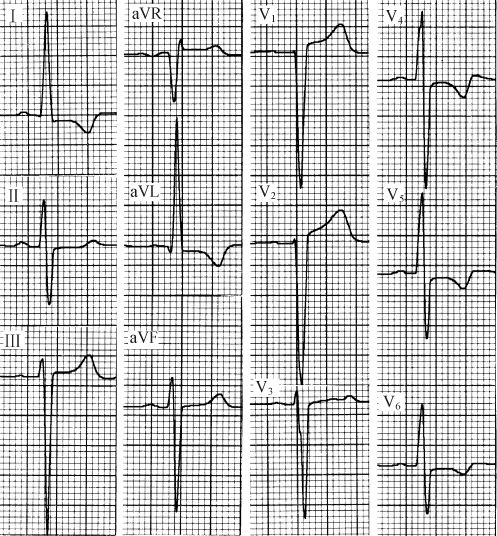
\includegraphics[width=3.22917in,height=2.21875in]{./images/Image00053.jpg}
\end{table}

当确认患者是上消化道出血后,需要迅速对下列问题作出判断,以便及时采取相应的处理。

\subsubsection{出血严重程度的估计和周围循环状态的判断}

对制定合理的治疗方案极为重要。

\subparagraph{失血量的判断与临床分级}

上消化道出血病情严重度与失血量呈正相关。一般而言,粪便隐血试验阳性提示每日失血量在5ml以上;出现黑粪者,每日出血量在50~70ml以上;如短期内出血量在250~300ml,多可导致呕血。因呕血与黑便混有胃内容物与粪便,而部分血液贮留在胃肠道内未排出,故难以根据呕血或黑便量精确判断出血量。常根据临床综合指标判断失血量的多寡,对出血量判断通常分为:大量出血(急性循环衰竭,需输血纠正者。一般出血量在1000ml以上或血容量减少20\%以上)、显性出血(呕血或黑便,不伴循环衰竭)和隐性出血(粪隐血试验阳性)。临床可以根据血容量减少导致周围循环的改变(伴随症状、脉搏和血压、化验检查)来判断失血量,并根据患者年龄、有无伴发病、失血量等指标将上消化道出血严重程度分为轻、中、重度三级(表\ref{tab13-2})。

\subparagraph{体位倾斜试验}

方法为先测平卧位时的血压(V\textsubscript{0}
)、脉搏(P\textsubscript{0}
),改为半卧位3分钟后,再测血压(V\textsubscript{1}
)、脉搏(P\textsubscript{1}
),符合下列条件之一者,提示失血量在1000ml以上。①V\textsubscript{0} −
V\textsubscript{1} >10mmHg;②P\textsubscript{1} − P\textsubscript{0} >
20次/分;③改半卧位后出现头晕、晕厥。必须在输液通路建立后才能进行,休克者禁作此试验。

\subparagraph{休克指数}

为脉搏(次/分)与收缩压(mmHg)的比值(P/SBP),指数正常值约为0.58。指数为1.0,大约失血800~1200ml(占血容量20\%~30\%);指数大于1.0,失血量1200~2000ml(占血容量30\%~50\%)。

\subparagraph{Hb、RBC和Hct的测定}

是估计失血量及决定输血量的重要参考指标。但在急性失血早期,由于血液浓缩及血液重新分布等代偿机制,上述指标可暂时无变化。一般出血3~4小时后,组织液渗入血管内补充血容量,患者可出现贫血,约24~72小时左右Hb稀释到最大限度。在连续测定中,三者迅速下降,表示继续出血,经输血纠正血容量后,与出血前比较,Hb每下降10g/L提示失血容量约400ml。

应指出的是,急性大出血严重程度的估计最有价值的指标是血容量减少所导致周围循环衰竭的临床表现,而周围循环衰竭又是急性大出血导致死亡的直接原因。因此,对急性消化道大出血患者,应将对周围循环状态的有关检查放在首位,并据此作出相应的紧急处理。血压和心率是关键指标,需进行动态观察,综合其他相关指标加以判断。如患者体位倾斜试验阳性,则提示血容量明显不足,是紧急输血的指征。如收缩压<
90mmHg,HR >
120次/分,伴有面色苍白,四肢湿冷,烦躁不安或神志不清则已进入休克状态,属严重大量出血(指3小时内需输血1500ml才能纠正其休克),需积极抢救。

\begin{table}[htbp]
\centering
\caption{上消化道出血病情严重程度分级}
\label{tab13-2}
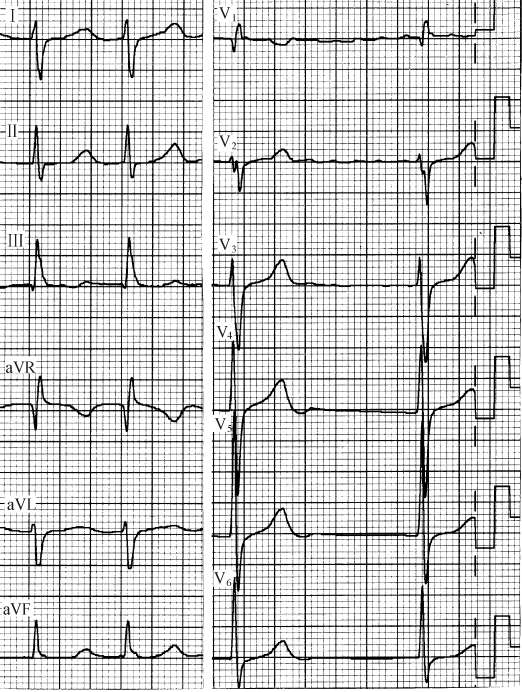
\includegraphics[width=6.65625in,height=0.91667in]{./images/Image00054.jpg}
\end{table}

\subsubsection{出血是否停止的判断}

临床上不能单凭Hb在下降或大便柏油样来判断出血是否停止或持续。因为一次出血后,Hb的下降有一定过程;而一次出血后柏油样大便持续天数受患者排便次数及出血量的影响。如每日排便1次,出血量在1000ml左右者,柏油样大便可持续1~3天,隐血试验阳性可达1周;若出血量在2000ml左右,柏油样大便可持续4~5天,隐血试验阳性达2周。应综合分析,特别是血压与脉搏的反复测定,直至恢复正常并趋稳定,尿量足(>
30ml/h),患者一般情况明显恢复者,方可认为已无活动性出血。有下列表现者,应认为有持续出血或再出血:①反复呕血或柏油样便次数及量增多,质稀薄,甚至排出暗红或鲜红色血便,伴肠鸣音活跃。②胃管抽出物有较多新鲜血。③周围循环衰竭的表现经积极补充血容量仍未见明显改善,或曾一度好转又很快恶化,中心静脉压仍有波动,稍稳定又再下降。④在补液量和排尿量足够的情况下,原无肾脏病变患者的BUN持续或再次升高。⑤Hb、RBC和Hct持续下降,血中网织红细胞持续增高。

肝硬化门静脉高压食管胃静脉曲张出血的防治共识(2008,杭州)关于EGVB继续出血或再出血的评估:①提示EGVB出血未控制的征象:72小时内出现以下表现之一者为继续出血。6小时内输血4个单位以上,生命体征不稳定。收缩压<
70mmHg,HR > 100次/分或心率增加> 20
次/分;间断呕血或便血,收缩压降低20mmHg以上或心率增加>
20次/分,继续输血才能维持Hb含量稳定;药物或内镜治疗后新鲜呕血,在没有输血的情况下,Hb含量下降30g/L以上。②提示EGVB再出血的征象:出现以下表现之一者为再出血。出血控制后再次有活动性出血的表现(呕血或便血;收缩压降低20mmHg以上或心率增加>
20
次/分;在没有输血的情况下,Hb含量下降30g/L以上)。早期再出血:出血控制后72小时~6周内出现活动性出血。迟发性再出血:出血控制6周后出现活动性出血。

\subsubsection{出血的病因诊断}

对上消化道大出血的患者,应首先纠正休克,然后尽快查找出血的部位与病因,以决定进一步的治疗措施和判断预后。一般通过询问病史、体检和必要的辅助检查,可明确出血的病因。

\subparagraph{病史与体检}

详询病史和系统体检,仍是出血病因与部位诊断的基础。约50\%的患者可据此作出病因诊断。慢性、周期性、节律性上腹痛多提示出血来自消化性溃疡,特别是在出血前疼痛加剧,出血后减轻或缓解,更有助于消化性溃疡的诊断。有服用非甾体抗炎药等损伤胃黏膜的药物或应激状态者,可能为急性糜烂出血性胃炎。对中年以上的患者近期出现上腹痛,伴有厌食、消瘦者,应警惕胃癌的可能性。既往有病毒性肝炎、血吸虫病或酗酒病史,并有肝病与门静脉高压的临床表现,可能是食管胃底静脉曲张破裂出血。尚应注意既往有无类似出血史、诊治情况等。

\subparagraph{急诊内镜检查}

急诊内镜检查是UGIB病因诊断中的首选方法。诊断正确率达80\%~94\%。急性上消化道出血的内镜检查有如下优点:①诊断正确率高:首先,内镜检查结合活检,既可明确出血部位,又可获得出血病变性质的诊断;其次,对一些上消化道钡餐检查不易发现的急性胃黏膜病变、贲门黏膜撕裂综合征、浅溃疡、胃黏膜毛细血管扩张症等,内镜可迅速作出诊断;第三,肝硬化合并上消化道出血病例,非静脉曲张破裂出血者占50\%左右,这仅能由内镜检查才能确诊。②提供预后的依据:如内镜下见溃疡基底喷血,溃疡基底血管、凝血块或红点等内镜征象可预示有再发出血的危险。③作为治疗手段:内镜诊断结合激光、高频电凝、喷洒止血剂以及给出血的曲张静脉内注射硬化剂等治疗性内镜的应用,使内镜检查不仅成为诊断工具,而且可作为止血治疗的方法。

\hypertarget{text00032.htmlux5cux23CHP1-13-1-4-4-2-1}{}
(1) NVUGIB的内镜检查:

①内镜检查能发现上消化道黏膜的病变,应尽早在出血后24~48小时内进行,并备好止血药物和器械。②内镜检查无食管胃底静脉曲张并在上消化道发现有出血病灶,NVUGIB诊断可确立。③内镜检查时根据溃疡基底特征,可用来判断病变是否稳定,凡基底有血凝块、血管显露等易于再出血。内镜检查时对出血灶病变应作Forrest分级(表\ref{tab13-3})。④应仔细检查贲门、胃底部、胃体垂直部、胃角小弯、十二指肠球部后壁及球后处,这些部位是易遗漏病变的区域。当检查至十二指肠球部未能发现出血病变者,应深插内镜至乳头部检查。发现有2个以上的病变,要判断哪个是出血性病灶。⑤有内镜检查禁忌证者不宜作此检查:如心率>
120次/分,收缩压< 90mmHg或较基础收缩压降低> 30mmHg、血红蛋白<
50g/L等,应先迅速纠正循环衰竭,血红蛋白上升至70g/L后再行检查。危重患者内镜检查时应进行血氧饱和度和心电、血压监护。

\begin{table}[htbp]
\centering
\caption{出血性消化性溃疡的 Forrest分级}
\label{tab13-3}
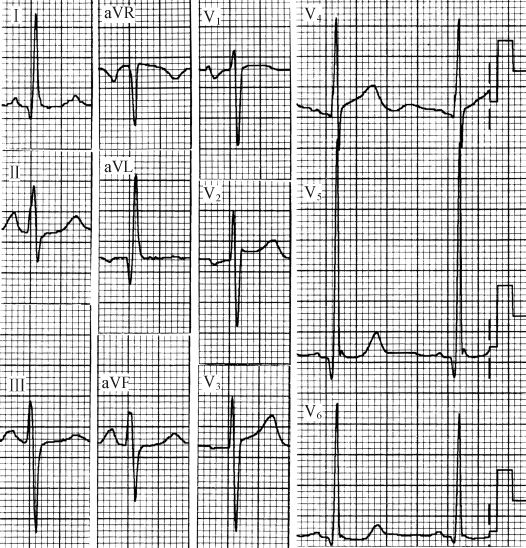
\includegraphics[width=3.26042in,height=1.5in]{./images/Image00055.jpg}
\end{table}

\hypertarget{text00032.htmlux5cux23CHP1-13-1-4-4-2-2}{}
(2) EGVB的内镜检查:

①内镜检查见有食管或胃曲张静脉出血,EGVB诊断即可成立;内镜检查时发现粗大曲张静脉和胃内血液而无其他可以识别的出血原因,EGVB诊断也可成立。②按食管静脉曲张形态及出血危险程度可将食管静脉曲张分轻、中、重3级。轻度(G\textsubscript{1}
):食管静脉曲张呈直线形或略有迂曲,无红色征(曲张静脉表面红斑、红色条纹和血疱)。中度(G\textsubscript{2}
):食管静脉曲张呈直线形或略有迂曲,有红色征或食管静脉曲张呈蛇形迂曲隆起但无红色征。重度(G\textsubscript{3}
):食管静脉曲张呈蛇形迂曲隆起且有红色征或食管静脉曲张呈串珠状、结节状或瘤状(不论是否有红色征)。③有内镜检查禁忌证者不宜作此检查(见前述)。

\hypertarget{text00032.htmlux5cux23CHP1-13-1-4-4-2-3}{}
(3) 内镜阴性患者的病因检查:

①仍有活动性出血的患者,应急诊行选择性腹腔动脉或肠系膜动脉造影,以明确出血部位和病因,必要时同时作栓塞止血治疗。②在出血停止,病情稳定后可作胃肠钡剂造影或放射性核素扫描(如\textsuperscript{99m}
锝标记患者的红细胞),但此检查特异性差。③对慢性隐性出血或少量出血者,可考虑作小肠镜检查。④对经各种检查仍未能明确诊断而出血不停者,病情紧急时可考虑剖腹探查,可在术中结合内镜检查,明确出血部位。

\subparagraph{X线钡餐检查}

目前已多为胃镜检查所替代。消化道大出血患者,因休克不能站立和充分变换体位,胃内潴留大量血液或血块影响钡餐充盈和病变征象观察,不易显示某些浅表病变如胃炎、急性胃黏膜病变等,仅能发现病变而不能确定是否为出血病变等,还可干扰以后内镜检查和血管造影检查,以及在活动性出血时,过早进行此项检查有加重出血的危险等因素,使急诊X线钡餐检查的实用性大大受到限制。因此,上消化道钡餐检查仅适用于出血已停止、生命体征平稳的上消化道出血患者。但对经胃镜检查出血原因未明、疑病变在十二指肠降段以下小肠段,则有特殊诊断价值。对某些解剖部位的改变,如胃黏膜脱垂、食管裂孔疝的诊断却优于一般胃镜检查。一般宜在出血完全停止3天后谨慎进行。

\subparagraph{血管造影}

对内镜检查无阳性发现或不适宜进行内镜检查者如有严重的心、肺并发症,且仍有活动性出血的患者可做选择性血管造影,对肠血管畸形、小肠平滑肌瘤等有很高的诊断价值,并可同时进行介入治疗。但忌用于严重动脉硬化、对碘剂过敏和老年患者。该检查的优点是:①灵敏性强:实验证明,出血量在0.5ml/min以上的消化道出血,在选择性血管造影连续摄影中即可见到造影剂从破裂血管外溢的X线征象。对慢性、隐源性活动性消化道出血是一种极有价值的诊断方法,阳性率一般为77\%~90\%。一般选择肠系膜上动脉及腹腔动脉造影已足够显示所要的范围。②具有精确的出血定位诊断价值:经出血相关区域血管注射造影剂,可精确显示出血部位和出血病变的供应动脉,为确定治疗提供了精确的解剖依据。③消化道内积血或血块不影响血管造影剂外溢的X线征象观察。④出血部位及其供应动脉显示后,立即经血管造影导管注射血管收缩剂或血管栓塞剂进行止血治疗。此外,门静脉造影(包括经脾穿刺门静脉造影、经肝穿刺门静脉造影以及经脐静脉插管门静脉造影等)除可以显示血管破裂部位、进行栓塞治疗外,还可以经导管测量门静脉压力诊断门脉高压症。

\subparagraph{放射性核素扫描}

经内镜及X线检查阴性的病例,可做放射性核素扫描。方法是采用核素(如\textsuperscript{99m}
锝)标记患者的红细胞后,再从静脉注入患者体内,当有活动性出血,且出血速度达到0.1ml/min,核素便可显示出血部位。注射一次\textsuperscript{99m}
锝标记的红细胞,可以监视患者消化道出血达24小时。本法缺点为出血部位定位不够确切,也不能确定出血病变的性质。

\subsubsection{预后估计与危险性分级}

约80\%~85\%急性上消化道出血患者除支持疗法外,无需特殊治疗出血可在短期内自然停止。仅有15\%~20\%患者持续出血或反复出血,而主要是这类患者由于出血并发症而导致死亡。如何早期识别再出血及死亡危险性高的患者,并给予加强监护和积极治疗,便成为急性上消化道出血处理的重点。提示预后不良、危险性增高的主要因素有:①高龄患者(>
60岁);②有严重伴随病(心、肺、肝、肾功能不全,脑卒中等);③本次出血量大或短期内反复出血;④特殊病因和部位的出血(如食管胃底静脉曲张破裂出血);⑤消化性溃疡伴有内镜下活动性出血,或近期出血征象。此外,EGVB出血48小时内肝静脉压力梯度(HVPG)>
20mmHg是其可靠的预后不良预测因子。

Rockall评分系统(表\ref{tab13-4})仍是目前临床广泛使用的评分依据,该系统依据患者年龄、休克状况、伴发病、内镜诊断和内镜下出血征象5项指标,将UGIB患者分为高危、中危或低危三级,积分≥5分者为高危,3~4分为中危,0~2分为低危。在Rockall评分系统中,若仅根据年龄、休克表现及伴发病三个指标评判疾病危险度,谓之为临床Rockall评分系统,可适用于无条件获取急诊内镜资料的基层医院;若同时有急诊内镜资料参与评估,谓之为完全Rockall评分系统。如出血患者,61岁,收缩压为105mmHg,心率为110次/分,胃镜下可见一巨大溃疡,活检示胃腺癌,附血凝块,无伴发病。则该患者Rockall积分=年龄(1)+心动过速(1)+无伴发病(0)+胃癌(2)+近期出血征象(2)=
6分,为高危患者。

Blatchford评分系统(表\ref{tab13-5})包含了BUN、Hb等实验室检查信息,其价值逐渐得到认可。

\begin{table}[htbp]
\centering
\caption{急性 UGIB患者的Rockall再出血和死亡危险性评分系统}
\label{tab13-4}
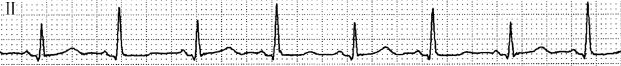
\includegraphics[width=6.67708in,height=1.83333in]{./images/Image00056.jpg}
\end{table}

注:\textsuperscript{※} 收缩压> 100mmHg,心率<
100次/分;\textsuperscript{△} 收缩压> 100mmHg,心率>
100次/分;\textsuperscript{▲} 收缩压< 100mmHg,心率> 100次/分

\begin{table}[htbp]
\centering
\caption{急性上消化道出血患者的 Blatchford评分}
\label{tab13-5}
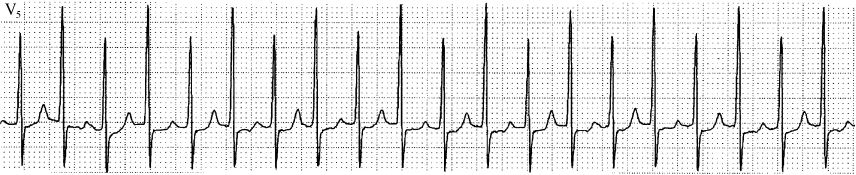
\includegraphics[width=3.32292in,height=3.75in]{./images/Image00057.jpg}
\end{table}

注:积分≥6分为中高危,< 6分为低危;1mmHg = 0.133kPa

\subsection{处理原则}

及早补充血容量、防治继续出血和再出血及病因治疗。其中,抗休克、迅速补充血容量应放在一切医疗措施的首位。

关于UGIB诊治流程,中国医师协会急诊医师分会制定的《急性上消化道出血急诊诊治专家共识》将上消化道出血的急诊诊治过程分为三个阶段,分别是紧急治疗期、病因诊断期和加强治疗期。紧急治疗期:患者入院6~48小时,治疗目标是控制急性出血、维持患者生命体征平稳并针对患者病情做出初步诊断及评估,治疗手段以药物治疗为主(PPI、生长抑素和抗菌药物联合用药)。病因诊断期:入院48小时内,急性出血得到控制,患者血流动力学稳定的情况下,行急诊内镜检查以明确病因并进行相应的内镜下治疗。无法行内镜检查的患者,可根据情况进行经验性诊断、评估和治疗。加强治疗期:入院后3~7天,治疗目标是病因治疗,预防早期再出血的发生。病因明确后,可根据不同病因采取不同的治疗手段。临床推荐采用以药物联合内镜治疗为主的综合治疗方法。

\subsubsection{一般措施}

患者应取平卧位休息,吸氧,严密观察患者的神色、血压、脉搏、出血量和尿量;保持静脉通道通畅,必要时作静脉切开。保持呼吸道通畅,避免呕血时引起窒息。烦躁不安者可给予镇静剂,如地西泮(安定)10mg肌注,对肝病患者忌用巴比妥类药物。呕血者宜暂禁食,但少量出血者宜进流质(因为胃内空虚产生饥饿的不正常的胃收缩不利于止血),活动性出血停止后可逐渐改变饮食的质与量。推荐对活动性出血或大出血患者宜常规放置胃管,其意义有:①可以观察出血情况,并可用冰盐水洗胃止血;②抽取胃内容物,减轻胃扩张,改善胃黏膜的循环,抽出积存在胃内的血液,能减轻日后吸收热和氮质血症,降低胃内酸度,防止凝血块被消化,有利于止血;③可通过胃管及时用药治疗;④预防吸入性肺炎;⑤鼻饲营养液。意识障碍和排尿困难者需留置尿管,危重大出血者必要时进行中心静脉压测定,老年患者常需心电、血氧饱和度、呼吸监护。

\subsubsection{迅速补充血容量}

迅速补充血容量是处理上消化道大出血的首要措施。立即查血型和配血,尽快建立有效的静脉输液通道,尽快补充血容量。在配血过程中,可先输平衡液或葡萄糖盐水。失血量较大(如减少20\%血容量以上)时,可输入血浆等胶体扩容剂。改善急性失血性周围循环衰竭的关键是要输血,一般输浓缩红细胞,严重活动性大出血考虑输全血。下列情况为紧急输血指征:①收缩压<
90mmHg(EGVB时< 80mmHg),或较基础收缩压降低幅度> 30mmHg;②Hb <
50~70g/L(EGVB时Hb < 50g/L),Hct < 25\%;③心率增快(>
120次/分)。输血量依失血量而定,原则上输血量应接近出血量。输血注意事项:①输血开始时,速度应加快,以尽快把收缩压升高至80~90mmHg水平,待血压稳定、病情改善后则减慢输血、输液速度,避免依赖升压药来维持血压。②避免输血、输液过多、过快,招致急性肺水肿,尤其是对有心、肺、肾疾患及老年患者。③防止枸橼酸中毒,一般每输血600~900ml可从静脉注入10\%葡萄糖酸钙10ml,以防低钙。④大量输注库存血时易引起高钾血症,应注意给予高渗葡萄糖,必要时加用适量胰岛素。⑤对肝硬化门脉高压静脉曲张破裂出血时,应输新鲜全血,除恢复血容量外,尚因其含有多种凝血因子和血小板成分,对止血有益;还可避免输库存血(含氨多)过多诱发肝性脑病。另外,输入的血约为失血量的2/3或3/4,以避免门静脉压力增高致再出血的危险。对于EGVB,以维持血流动力学稳定并使Hb维持在80g/L以上;过度输血或输液可能导致继续或重新出血;避免仅用氯化钠溶液补足液体,以免加重或加速腹水或其他血管外液体的蓄积;必要时应及时补充凝血因子、凝血酶原复合物等;血小板<
50 × 10\textsuperscript{9}
/L者,可输注血小板。对于急性大量出血者,应尽可能施行中心静脉导管置管和中心静脉压监测,以指导液体复苏。在补足液体的前提下,如血压仍不稳定,可以适当地选用血管活性药物(如多巴胺)以改善重要脏器的血液灌注。血容量充足的指征:①神志清楚或好转,无明显脱水貌;②收缩压90~120mmHg;③脉搏<
100次/分;④尿量> 40ml/h,血钠< 140mmol/L。

\subsubsection{非静脉曲张性上消化道出血(nonvariceal UGIB,NVUGIB)的止血措施}

NVUGIB是指除食管胃底静脉曲张破裂出血以外的其他病因引起的上消化道出血。包括消化性溃疡、急性糜烂出血性胃炎、胃泌素瘤、食管裂孔疝等所致的出血。止血措施主要有:

\subparagraph{内镜下止血}

起效迅速、疗效确切,应作为首选。可根据医院的设备和病变的性质选用,常用方法有:

\hypertarget{text00032.htmlux5cux23CHP1-13-1-5-3-1-1}{}
(1) 对出血灶喷洒止血药物:

内镜下直接对出血灶喷洒止血药物,对局部渗血疗效较好,对动脉性出血疗效较差。常用的药物有去甲肾上腺素溶液、孟氏液、注射用血凝酶、凝血酶等。

\hypertarget{text00032.htmlux5cux23CHP1-13-1-5-3-1-2}{}
(2) 局部注射法:

当内镜检查发现喷射性出血或血管显露时,可用局部注射法止血。常用的注射剂有肾上腺素溶液、凝血酶、无水酒精、高渗盐水等。其方法是在出血血管周围1~2mm处选3~4点,每点注入0.1~0.3ml。本法安全、有效,且可反复应用。

\hypertarget{text00032.htmlux5cux23CHP1-13-1-5-3-1-3}{}
(3) 激光照射法:

可供止血的激光有氩激光(Argon)和镱-铝-石榴石激光(Nd-YAG)两种。后者功率大,止血效果好。止血机制是由于光凝作用,使照射局部组织蛋白凝固,小血管内血栓形成。止血成功率在80\%~90\%。其并发症有胃肠穿孔、出血及胃肠胀气等。

\hypertarget{text00032.htmlux5cux23CHP1-13-1-5-3-1-4}{}
(4) 微波凝固法:

将微波经内镜导入出血部位,使产生热凝固,达到止血目的。其优点是,操作简便,并可将微波针状电极直接插入组织内治疗,插入组织的深度易控制,因而止血目标确切,安全性大。

\hypertarget{text00032.htmlux5cux23CHP1-13-1-5-3-1-5}{}
(5) 高频电凝止血法:

应用高频电流的热效应,使局部组织蛋白变性达到止血,迅速止血率达87\%~96\%。主要用于血管显露性出血及有直接出血征象的出血性病变。方法是用凝固电流在出血灶周围电凝,使黏膜下层或肌层的血管凝缩,最后电凝出血血管。有出血、溃疡、穿孔等并发症。近年来为了提高电凝止血的安全性和止血效果,研制出各种形状的及带喷水孔的单极电凝头、双极电凝头及四头双极电凝探头。

\hypertarget{text00032.htmlux5cux23CHP1-13-1-5-3-1-6}{}
(6) 热探头凝固法:

是利用热探头的高温(150℃)接触出血灶,使其组织蛋白质凝固而达到止血。此法疗效确切、安全、简单。

\hypertarget{text00032.htmlux5cux23CHP1-13-1-5-3-1-7}{}
(7) 放置止血夹法:

内镜直视下放置止血夹子,把出血的血管夹住止血,伤口愈合后此金属夹子自行脱落随粪便排出体外,此法止血既安全又有效。适用于消化性溃疡、急性胃黏膜病变的出血治疗,尤其在小动脉出血时用该法甚佳。

\subparagraph{制酸药物的应用}

胃酸在上消化道出血中起重要作用,抑制胃酸分泌及中和胃酸可达到止血的效果。制酸药止血的关键是使胃内pH维持在>
6,这样,既可促进血小板聚集和纤维蛋白凝块的形成,避免血凝块过早溶解,有利于止血和预防再出血,又可治疗消化性溃疡等病变。尤适用于消化性溃疡、急性胃黏膜病变、胃泌素瘤、食管裂孔疝等所致的出血。常用制剂有:

\hypertarget{text00032.htmlux5cux23CHP1-13-1-5-3-2-1}{}
(1) 中和胃酸药:

将胃内容物抽尽,用氢氧化铝凝胶60ml经胃管注入,15分钟后测胃液pH,若<
6,再注入60ml,以后每小时测pH1次,使其值维持在> 6。

\hypertarget{text00032.htmlux5cux23CHP1-13-1-5-3-2-2}{}
(2) H\textsubscript{2} 受体阻滞剂(H\textsubscript{2} RA):

目前临床上常用的有:第一代的西咪替丁(cimetidine,甲氰咪胍)、第二代的雷尼替丁(ranitidine)和第三代的法莫替丁(famotidine)。由于后两者不仅抗酸作用强(雷尼替丁比西咪替丁强5~8倍,法莫替丁比西咪替丁强30~100倍),作用时间更持久,且毒副作用相对较轻,应作为首选。可用雷尼替丁50mg缓慢静脉注射,每6~12小时1次,或用150~300mg加入液体中持续静滴;法莫替丁20mg溶入生理盐水或葡萄糖液20ml中,缓慢静脉注射,每日2次。

\hypertarget{text00032.htmlux5cux23CHP1-13-1-5-3-2-3}{}
(3) 质子泵抑制剂(proton pump inhibition,PPI):

可抑制胃壁细胞的H\textsuperscript{+} -K\textsuperscript{+}
-ATP酶,从而抑制胃酸的分泌。其抑制胃酸作用远强于H\textsubscript{2}
RA,几乎完全抑制酸分泌,持续用药无耐受性,且作用持久、递增,3~5天达稳态,胃内pH维持平稳。大剂量PPI可减少高危患者再出血率,且总费用降低,是治疗NVUGIB的首选止血药物。加拿大NVUGIB共识会议推荐内镜止血成功后应用PPI,在待行内镜检查时也应给予大剂量PPI,并认为H\textsubscript{2}
RA不能减少再出血率及病死率,不提倡用H\textsubscript{2}
RA止血。PPI常用制剂有:奥美拉唑(omeprazole,又名洛赛克,Losec)、泮托拉唑(pantoprazole)和兰索拉唑(lansoprazole)等。PPI给药方法及剂量:高危患者应静脉给药,如奥美拉唑静脉推注80mg后,以8mg/h输注72小时;如低危患者可口服给药,如奥美拉唑20mg,每6小时一次,持续5天。

\subparagraph{奥曲肽(octreotide)}

商品名善得定(Sandostatin),是人工合成的生长抑素类似品。能抑制胃酸、胃蛋白酶和胃泌素分泌,促进胃黏膜生长,能选择性引起内脏循环血流量减少和门脉压下降。用法:100μg皮下注射,每日2~4次。

\subparagraph{去甲肾上腺素}

可使胃肠黏膜出血区域的小动脉强烈收缩,减少局部血流量,并能减少胃酸分泌,有类似迷走神经切断的作用;同时因可降低门脉压,故亦用于食管静脉曲张破裂出血。用法有二:①口服或胃管内灌入:用去甲肾上腺素8mg加入冷生理盐水100~200ml中为1次量,口服或由胃管内灌入,每0.5小时1次,共2~4次;若有效,可再改为1小时1次,共4~6小时,以后每2小时1次共4~6小时。若无效,则不用。②腹腔灌注:以细长穿刺针作腹腔穿刺,注入含去甲肾上腺素8mg的生理盐水100ml,然后来回转动患者腹部,出血可迅速停止。本法适用于有腹水者,以免注入组织内引起缺血性坏死。

\subparagraph{注射用血凝酶(立止血,reptilase)}

是酸性止血剂,含有如凝血激酶和凝血酶样物质,可直接作用于内、外源性凝血系统形成凝血活酶,促进凝血酶的形成而起到凝血作用。用法:首次静注与肌注各1kU,继而每日肌注1kU。无明显毒副作用。

\subparagraph{凝血酶(thrombin)}

本品是从猪血提取、精制而得的凝血酶无菌制剂。能直接作用于出血部位的纤维蛋白原,使其转变为纤维蛋白,促使血液凝固、填塞出血点而止血;尚有促进上皮细胞的有丝分裂而加速创伤愈合的作用。其特点是局部止血迅速,疗效显著,无明显不良反应,但出现过敏反应时,应立即停用。首次剂量宜大(8000U~2万U),溶入50~100ml生理盐水或牛奶、豆汁内口服或胃管内注入,每2~6小时1次,应用次数视病情而定。凝血酶遇热或在酸性环境中均易失去活性,故溶液温度不要超过37℃,同时给予抑酸药物(如H\textsubscript{2}
受体阻滞剂、质子泵抑制剂)以便得以发挥最大作用。本品切忌血管内或肌内注射。

\subparagraph{其他止血药物}

以下止血药物对NVUGIB的确切效果未能证实,不作为一线药物使用。应避免滥用止血药。可酌情选用的有:①维生素K:能促进凝血酶原及凝血因子Ⅷ、Ⅵ、Ⅳ、Ⅹ在肝内合成。可用维生素K\textsubscript{1}
10mg肌注,每日2次;或维生素K\textsubscript{4}
口服4mg,每日3次;②肾上腺色腙(安络血):可增强受损毛细血管的修复能力,从而达到止血目的。10mg肌注,每天2次;或5~10mg口服,每天3~4次。③酚磺乙胺(止血敏):有增强血小板的作用。0.5~1.0g口服,每天3次;或0.5g肌注或静注。④氨甲苯酸(止血芳酸)、氨基己酸:能抑制纤溶酶原的激活因子和抑制纤维蛋白的溶解。⑤中药:云南白药、三七粉、白及粉、血余炭等均有防腐生肌、凉血止血的作用,中成药如止血散(白及、煅瓦楞、三七、甘草)、止血粉(白及、蒲黄、地榆、甘草)、止血汤(仙鹤草、地榆炭、白及、生槐花)等可酌情辨证选用。

\subparagraph{选择性血管造影及栓塞治疗}

选择性胃左动脉、胃十二指肠动脉、脾动脉或胰十二指肠动脉血管造影,针对造影剂外溢或病变部位经血管导管滴注血管升压素或去甲肾上腺素,导致小动脉和毛细血管收缩,使出血停止。无效者可用明胶海绵栓塞。

\subparagraph{手术治疗}

诊断明确但药物和介入治疗无效者,诊断不明确、但无禁忌证者,可考虑手术,结合术中内镜止血治疗。约10\%的胃十二指肠溃疡大出血患者需急症手术止血,手术指征为:①出血速度快,短期内发生休克,或较短时间内(6~8小时)需要输入较大量血液(>
800ml)方能维持血压和Hct者;②年龄在60岁以上伴动脉硬化症者自行止血机会较小,对再出血耐受性差,应及早手术;③近期发生过类似的大出血或合并穿孔或幽门梗阻;④正在进行药物治疗的胃十二指肠溃疡患者发生大出血,表明溃疡侵蚀性大,非手术治疗难以止血;⑤内镜检查发现动脉搏动性出血,或溃疡底部血管显露再出血危险很大。急诊手术应争取在出血48小时内进行,胃溃疡较十二指肠溃疡再出血概率高3倍,应争取及早手术。

\subparagraph{原发病的治疗}

对出血的病因比较明确者,如幽门螺杆菌阳性的消化性溃疡患者,应予抗幽门螺杆菌治疗及抗溃疡治疗。需要长期服用非甾体抗炎药者一般推荐同时服用PPI或黏膜保护剂。

非静脉曲张性上消化道出血诊治流程见图\ref{fig13-1}。

\subsubsection{食管胃静脉曲张出血的止血治疗}

肝硬化门脉高压症患者发生上消化道出血,并不全是由食管胃底静脉曲张破裂所致,而是多种因素共同作用的结果。因此,它的治疗仍应以上述治疗措施为基础。EGVB活动性出血的止血措施主要有内镜治疗、血管活性药物、经颈静脉肝内门体分流术(transjugular
intrahepatic portosystemic
shunt,TIPS)、外科手术和双气囊堵塞压迫等。其作用机制、运用方法及注意事项等有关内容,详见本书第116章第1节“肝硬化并上消化道出血”部分。

\subsubsection{预后}

据临床资料统计,约80\%~85\%急性上消化道大量出血的患者除支持疗法外,无需特殊治疗,出血可在短期内自然停止。仅有15\%~20\%患者持续出血或反复出血,常因出血并发症而导致死亡。如何早期识别再出血及死亡危险性高的患者,并予加强监护和积极治疗,便成为急性上消化道大量出血处理的重点。提示预后不良危险性增高的主要因素有:①高龄患者(>
60岁);②有严重伴随病(心、肺、肝、肾功能不全、脑卒中等);③本次出血量大或短期内反复出血;④特殊病因和部位的出血(如食管胃底静脉曲张破裂出血);⑤消化性溃疡伴有内镜下活动性出血,或近期出血征象。

\begin{figure}[!htbp]
 \centering
 \includegraphics[width=4.23958in,height=3.55208in]{./images/Image00058.jpg}
 \captionsetup{justification=centering}
 \caption{急性非静脉曲张性上消化道出血诊治流程}
 \label{fig13-1}
  \end{figure} 

PPIs:质子泵抑制剂;H\textsubscript{2} RA:H\textsubscript{2} 受体拮抗剂

\protect\hypertarget{text00033.html}{}{}

\section{下消化道出血}

下消化道出血(lower gastrointestinal
hemorrhage)是指屈氏韧带以下的小肠或大肠出血。依其出血量大小、速度和快慢等可分为三类:①慢性隐性出血:肉眼不能观察到便血,仅有大便隐血试验阳性,常以不明原因贫血就诊或普查时发现。②慢性少量显性出血(亚急性出血):表现为间歇性或持续性肉眼可见的少量显性便血,可呈鲜红色、果酱样或柏油样黑粪,无循环衰竭表现。③急性大量出血:短期内排出大量鲜红或暗红色血便,伴血压下降等休克症状,常需输血治疗者。多数下消化道出血相对缓慢,或呈间歇型,约80\%的出血能自行停止。在治疗上除了止血、补充血容量以外,寻找下消化道出血部位、疾病性质进行原发病病因治疗最为重要。

下消化道范围广,出血病因繁多,分类各异。如按病变部位可分为:①小肠疾病:小肠肿瘤、黑色素-胃肠息肉综合征、克罗恩病(Crohn病)、小肠憩室与Meckel憩室、肠套叠、小肠血管畸形、急性出血性坏死性肠炎、缺血性小肠炎和肠结核等。②大肠疾病:溃疡性结肠炎、结肠息肉、结肠憩室、菌痢、阿米巴痢疾、结肠癌、克罗恩病、缺血性结肠炎、结肠子宫内膜异位症、结肠结核及肠套叠、结肠血管畸形等。③直肠疾病:直肠溃疡、非特异性炎症、肿瘤、息肉、放射性直肠炎和腹盆腔邻近脏器恶性肿瘤或脓肿侵及直肠等。④肛管疾病:痔、肛裂、肛瘘。此外,还有全身性疾病累及肠道。国内资料引起下消化道出血的最常见病因为大肠癌和大肠息肉,其次为肠道炎症性疾病(其中肠伤寒、肠结核、溃疡性结肠炎、克罗恩病和坏死性小肠炎有时可发生大量出血)和血管病变,憩室引起的出血少见。但在西方国家,血管病变和消化道憩室是下消化道出血最常见病因,其次为结肠肿瘤和炎症性肠病。

\subsection{诊断思路}

\subparagraph{下消化道出血的确立}

首先要排除口腔、鼻咽、喉、气管、支气管、肺等部位的出血被吞咽后由肛门排出的可能性,还要与下列情况区别:①口服某些中草药、兽炭、铁剂、铋剂时,大便可呈暗褐色或黑色,但隐血试验阴性;②食用过多的肉类、猪肝、动物血后大便可变暗褐色,隐血试验呈阳性,但素食后即转呈阴性;③口服酚酞制剂,大便有时呈鲜红色,不注意时易误诊为大量便血。

排除了上述因素后,要确定是否为下消化道出血,大便的色泽和量是重要的线索,通常大便呈鲜红色或暗红色者,即可确诊。但如为暗红色大量血便或仅表现为黑便或大便隐血阳性时,则应与上消化道出血鉴别。此时应常规行胃十二指肠镜检查,若未发现病变,大致可除外上消化道出血。

下述几点有助于下消化道出血的诊断:①病史中多伴有下腹痛或腹部有包块,排便异常伴便血史,出血前常有中下腹不适、下坠或便意。②大便常为鲜红、暗红、果酱样,少数为黑便,无呕血。③下消化道出血时胃管内无咖啡色的液体和暗红色的血液被抽出。④来自高位小肠的出血可能有血BUN升高,而结肠出血常不升高;上消化道出血时血BUN升高较下消化道出血时明显。⑤结直肠出血,常表现为鲜血便或是暗红的血便,血与大便相混,可有便后滴血,亦可表现为脓血便。⑥小肠出血常为暗红果酱样便,亦可为黑便,偶有血水样便。⑦大肠出血常伴有下腹痛、腹泻、里急后重等症状,而小肠出血常表现为脐周疼痛。

\subparagraph{估计出血速度和出血量}

下消化道出血确定后,估计出血速度和出血量甚为重要。判断患者出血速度和出血量的最终标准取决于为恢复和维持血容量所需的输血量和速度。在此之前,则可根据有无循环障碍及其程度、Hct和Hb变化作出初步估计。

\subparagraph{确定是否由全身性疾病所致下消化道出血}

全身性疾病所致的下消化道出血有相应疾病的全身表现。血液系疾病、血管疾病、肝脏疾病和某些中毒性疾病常伴有凝血与止血功能障碍,有凝血因子缺乏、血小板质或量改变、血管脆性增加、血管收缩障碍的实验室发现。相反,多数传染性疾病及中毒性疾病下消化道出血的主要原因是肠黏膜、黏膜下血管受损的后果。血液检查、骨髓检查、凝血机制检查等有助于诊断。

\subparagraph{出血部位的判断}

下消化道出血最常见的部位是乙状结肠,占50\%左右。其他部位出血频率依次为直肠、降结肠、横结肠、升结肠、盲肠、小肠。根据出血类型常可对出血部位作出初步判断:仅大便隐血阳性者,若排除了上消化道出血,则多为右侧结肠和小肠出血;少量显性出血,则主要是结肠、直肠出血;鲜红或暗红色血便,以左半结肠和直肠为主;果酱色或咖啡色血便则多为右半结肠出血。虽右半结肠和小肠出血的发生率较低,但较易发生急性大出血。上位结肠出血时,血与大便常混杂;乙状结肠和直肠出血时,常有新鲜血液附着于成形大便的表面。血在大便后滴下,与粪便不相混杂者,虽多见于内痔、肛裂,但也可见于直肠息肉和直肠癌,应予以注意。

\subparagraph{出血病因的诊断}

病史与体检是出血病因诊断中最重要的基础工作。

\hypertarget{text00033.htmlux5cux23CHP1-13-2-1-5-1}{}
(1) 既往史:

①反复小量显性出血史,提示痔、息肉、憩室等。②大便习惯改变或大便变细有切迹,应警惕结肠、直肠肿瘤。③反复血性腹泻史提示炎症性肠病可能。④曾患疾病与用药:曾患肺结核者应考虑肠结核;动脉硬化、心律失常、口服避孕药者应考虑缺血性结肠炎;风湿性疾病、白血病、出血性疾病、尿毒症、急性胰腺炎等病程中发生出血,多由于原发病引起的肠道病变;应用抗生素过程中出血应考虑假膜性肠炎、出血性结肠炎;便血前数月或数年曾接受腹部放射治疗者应考虑放射性结肠炎。

\hypertarget{text00033.htmlux5cux23CHP1-13-2-1-5-2}{}
(2) 便血特点与伴随症状:

①脓血黏液便伴里急后重或坠胀感,大便次数增多,应考虑痢疾和直肠癌可能。②中小量出血,色较红而呈间断性附于大便表面,要注意息肉出血之可能。③便血伴剧烈腹痛者,尤其是老年人心血管病患者,应警惕肠系膜血管栓塞;便血伴发热应考虑感染性肠炎、炎症性肠病、肠结核、肠伤寒、出血性坏死性肠炎、血液系疾病(白血病、恶性组织细胞病、恶性淋巴瘤等)等;便血伴腹块或不全性肠梗阻应考虑肿瘤、肠结核、Crohn病、肠套叠等;便血伴腹壁瘘管(或内瘘管),见于Crohn病、肠结核、癌、放线菌病。

\hypertarget{text00033.htmlux5cux23CHP1-13-2-1-5-3}{}
(3) 年龄与病因:

下消化道出血的病因与年龄有关:①婴儿和儿童:以Meckel憩室最多见,幼年性息肉次之,其他有炎症性肠病、肠套叠等。②青少年和成年人:在青少年时期,Meckel憩室依然是最常见病因,其次是炎症性肠病和息肉;随年龄增长癌肿比例显著增高。③老年人:以癌肿、息肉多见,其次为慢性结肠炎症、结肠血管扩张、结肠憩室等。

\hypertarget{text00033.htmlux5cux23CHP1-13-2-1-5-4}{}
(4) 出血部位与病因:

①直肠、乙状结肠:以息肉、癌、溃疡性结肠炎、单纯性溃疡、菌痢、阿米巴肠炎、放射性肠炎多见;②结肠脾曲、降结肠、乙状结肠:除息肉、癌外,易发生缺血性结肠炎;③右侧结肠:憩室、血管畸形、肠结核、Crohn病;④回盲部(回肠末段至升结肠始段):除癌、息肉外,类癌、Crohn病、单纯性溃疡、肠结核、鞭虫病、阿米巴肠炎、肠套叠、Meckel憩室、肠伤寒、沙门菌肠炎等。

\hypertarget{text00033.htmlux5cux23CHP1-13-2-1-5-5}{}
(5) 肛门视诊和直肠指检:

下消化道出血病因诊断的第一步,应采用简便易行的肛门视诊和直肠指诊,以发现或排除痔、肛裂,以及大部分直肠癌和息肉等常见的出血病因。

\hypertarget{text00033.htmlux5cux23CHP1-13-2-1-5-6}{}
(6) 内镜检查:

结肠镜检查是诊断大肠和回肠末端病变的首选检查方法。宜尽量在出血停止后近期或出血间歇期进行。对于出血灶的诊断,以窥视下直接见到活动性渗血最可靠。

\hypertarget{text00033.htmlux5cux23CHP1-13-2-1-5-7}{}
(7) X线钡剂造影检查:

一般要求在大出血停止至少3天后进行。主张双重气钡造影。其优点是基层医院已普及,患者易接受。缺点是对较平坦病变、广泛而较轻炎症性病变易漏诊,有时无法确定病变性质。对X线钡剂灌肠检查阴性的下消化道出血患者需进行结肠镜检查,已作结肠镜全结肠检查患者则不强调本项检查。

\hypertarget{text00033.htmlux5cux23CHP1-13-2-1-5-8}{}
(8) 胶囊内镜或双气囊小肠镜检查:

适用于常规内镜检查和X线钡剂造影不能确定出血来源的不明原因出血,出血活动期和静止期均可进行,可视病情和医疗条件选用。

\hypertarget{text00033.htmlux5cux23CHP1-13-2-1-5-9}{}
(9) 放射性核素扫描或选择性腹腔动脉造影:

必须在活动性出血时进行。主要用于急诊结肠镜检查不能确定出血来源的不明原因出血。放射性核素扫描检查的特点是简便敏感,出血量约0.1ml/min时即有阳性显示;缺点是对出血不能准确定位。常用本法初步确定出血部位,为进一步作血管造影提供线索。此外,利用\textsuperscript{99m}
Tc腹部扫描可用于诊断有胃黏膜异位的先天性病变,如Meckel憩室、肠重复畸形等。对持续大出血患者经上述检查不能明确出血灶时,应及时作选择性肠系膜上动脉造影,因肠系膜上动脉支配全部小肠和右侧结肠。约50\%~80\%的憩室出血和全部血管畸形出血均发生于右侧结肠。如肠系膜上动脉造影阴性,应再作肠系膜下动脉和腹腔动脉造影。血管造影可显示低至0.5ml/min的出血,此外还可显示肿瘤血管和血管畸形。成功的血管造影约于2/3的病例可显示肠出血来源。

\hypertarget{text00033.htmlux5cux23CHP1-13-2-1-5-10}{}
(10) 手术探查:

如上述检查仍不能明确出血灶,持续大出血危及患者生命,必须手术探查。术中内镜是明确诊断不明原因消化道出血,尤其是小肠出血的可靠方法。

不明原因消化道出血(obscure gastrointestinal bleeding,
OGIB)是指常规内镜检查(胃镜和结肠镜)不能确定出血来源的持续或反复消化道出血,多为小肠出血(如小肠的肿瘤、Meckel憩室和血管病变等),是消化道出血诊断的难点。OGIB的诊断步骤:在出血停止期,先行小肠钡剂检查;在出血活动期,应及时作放射性核素扫描或选择性腹腔动脉造影;若上述检查结果阴性则选择胶囊内镜或及双气囊小肠镜检查;出血不止危及患者生命者行手术探查,探查时可辅以术中内镜检查。

\subsection{处理原则}

下消化道出血主要是病因治疗,大出血时应积极抢救。

\subparagraph{一般措施}

一般急救措施与补充血容量同上消化道出血一样。一般措施包括应用注射用血凝酶、静滴血管加压素、生长抑素、肾上腺色腙(安络血)、酚磺乙胺等药物。

\subparagraph{局部止血措施}

对结肠出血,可给予冰盐水去甲肾上腺素液(去甲肾上腺素8mg加入100~200ml生理盐水中)、孟氏液、凝血酶等进行灌肠。

\subparagraph{内镜下止血措施}

包括内镜下向出血病灶喷洒止血药物、高频电凝止血、激光止血、息肉电凝止血、黏膜和黏膜下注射硬化剂等措施止血。

\subparagraph{放射性介入治疗}

在做选择性动脉造影时,若发现造影剂有渗出,即可通过导管给予血管加压素滴注,0.1~0.4U/min。对结肠出血不能自发地停止或血管加压素输注无效的病例,可施行栓塞治疗。在荧光透视下作超选择性插管,将管端插入出血灶近端几厘米处,注入明胶海绵碎片或自体凝血块,可将出血动脉栓塞、制止出血。

\subparagraph{手术治疗}

经内科保守治疗仍出血不止危及生命,无论出血病变是否确诊,均是紧急手术的指征。此外,对下列情况可行手术治疗:①对Meckel憩室、肠重复畸形、恶性肿瘤、先天性动静脉畸形(包括结肠血管扩张)等皆可手术切除。②息肉病、家族性息肉病或有高度癌变倾向的息肉可手术切除。但一般息肉可经纤维结肠镜电凝切除。③溃疡性结肠炎引起的大出血是次全或全结肠切除的手术指征;Crohn病时如病变局限也可作局限性肠切除。

下消化道出血的处理程序如图\ref{fig13-2}。

\protect\hypertarget{text00034.html}{}{}

\section{不明原因消化道出血}

不明原因消化道出血(obscure gastrointestinal
bleeding,OGIB)是指常规的消化道内镜(包括检查食管至十二指肠降段的上消化道内镜与肛直肠至回盲瓣的结肠镜检查)和常规钡餐检查不能明确病因的持续或反复发作的出血。可分为不明原因的隐性出血和不明原因的显性出血。前者表现为反复发作的缺铁性贫血和大便隐血阳性,而后者则表现为黑便、血便等肉眼可见的出血。OGIB占消化道出血的3\%~5\%。

根据国内外文献报道,40岁以下患者OGIB的病因多为小肠肿瘤、Meckel憩室、Dieulafoy病、遗传性息肉综合征或克罗恩病等;而40岁以上患者则多见于血管病变、非甾体类抗炎药相关性溃疡、大的食管裂孔疝囊内的糜烂(Cameron糜烂)和其他少见病因如主动脉肠瘘等。

\begin{figure}[!htbp]
 \centering
 \includegraphics[width=3.98958in,height=3.90625in]{./images/Image00059.jpg}
 \captionsetup{justification=centering}
 \caption{下消化道出血的处理程序}
 \label{fig13-2}
  \end{figure} 

\subsection{诊断思路}

\hypertarget{text00034.htmlux5cux23CHP1-13-3-1-1}{}
(一) 诊断方法与选择

\subparagraph{病史和体格检查}

对OGIB患者首先应仔细询问病史(包括目前症状、既往史、用药史、家族史等)。如果患者有消瘦或梗阻症状,提示小肠疾病的可能性大;而老年患者如有肾病或结缔组织病等,则血管病变的风险较高。详细可靠的病史和体格检查有助于减少漏诊率。

\subparagraph{内镜检查}

\hypertarget{text00034.htmlux5cux23CHP1-13-3-1-1-2-1}{}
(1) 常规内镜:

为OGIB的必需检查。对OGIB的内镜检查,应请有经验的内镜医师复核。初次检查阴性的患者必要时可重复内镜检查,有助于提高诊断率及减少漏诊率。初次检查时易被漏诊的病变有血管扩张、Cameron溃疡和位于盲区的消化性溃疡、息肉等。

\hypertarget{text00034.htmlux5cux23CHP1-13-3-1-1-2-2}{}
(2) 胶囊内镜:

目前,胶囊内镜已成为小肠疾病的重要检查技术。对OGIB患者,胶囊内镜的诊断阳性率为66\%~76\%,并且对于持续性出血的OGIB诊断阳性率高于间歇性出血的OGIB,对于显性出血的OGIB诊断阳性率高于隐性出血的OGIB。但胶囊内镜的缺点为不能进行治疗,遇肠段狭窄或梗阻时可能被嵌顿,出血量较多时视野不清等。

\hypertarget{text00034.htmlux5cux23CHP1-13-3-1-1-2-3}{}
(3) 小肠镜:

小肠镜是目前观察小肠病变较好的检查方法,并已成为OGIB的重要手段。传统推进式小肠镜仅能插入深度在幽门下50~150cm不等,患者依从性较差,操作技术要求高。近年来发展的双气囊电子小肠镜具有插入深度好、诊断率高的特点。它利用固定于镜身前端和外套管的2个气囊交替充气和放气,有经口、经肛两种检查方法,并且可以进行黏膜活组织检查,对小肠出血的诊断率在60\%以上。因此,双气囊小肠镜检查对于OGIB有较高的诊断和治疗价值。

\subparagraph{影像学检查}

\hypertarget{text00034.htmlux5cux23CHP1-13-3-1-1-3-1}{}
(1) 全小肠钡剂造影(small bowel follow through,SBFT):

SBFT对OGIB的诊断率不高,且假阴性率较高,因此较少使用。但是若怀疑肿瘤、克罗恩病、肠结核等可考虑行SBFT。

\hypertarget{text00034.htmlux5cux23CHP1-13-3-1-1-3-2}{}
(2) 小肠钡剂灌肠:

小肠钡剂灌肠是经口或鼻插管至近端小肠后将钡剂导入,对小肠进行摄片和透视的方法。其对OGIB的诊断率为10\%~21\%,优于SBFT。

\hypertarget{text00034.htmlux5cux23CHP1-13-3-1-1-3-3}{}
(3) 血管造影:

血管造影是一项有创性检查,有助诊断显性OGIB(出血速率大于0.5ml/min)。与核素扫描相比,血管造影定位相对准确,且能直接进行血管栓塞治疗,止血率高,但出血复发率也高。血管造影的并发症有肾功能衰竭和缺血性肠炎等。

\hypertarget{text00034.htmlux5cux23CHP1-13-3-1-1-3-4}{}
(4) CT和MRI:

螺旋CT血管造影是一项新兴的检查技术,将导管插至腹主动脉并注入造影剂,如造影剂外渗至肠腔内形成大片高密度区,即可确定出血位置。对于常规血管造影阴性的OGIB患者可行CT血管造影。利用CT
或MRI进行小肠造影能同时进行肠腔和肠壁结构的观察。但目前临床经验较少,有待进一步研究。

\subparagraph{核素扫描}

核素扫描有助于诊断显性OGIB(出血速率保持在0.1~0.4ml/min)。可采用\textsuperscript{99m}
Tc标记的红细胞或\textsuperscript{99m}
Tc标记的胶体硫进行扫描,前者更为常用。通过核素扫描可以大致定位出血点,但有一定的假阳性率及假阴性率,需要鉴别血池区积血是否为原发出血灶。

\subparagraph{外科手术和术中内镜检查}

外科手术是OGIB最后考虑的剖腹探查手段。单纯剖腹探查风险较大且成功率低。而外科手术结合术中内镜检查可提高诊断率至50\%~100\%。

\begin{figure}[!htbp]
 \centering
 \includegraphics[width=4.19792in,height=2.86458in]{./images/Image00060.jpg}
 \captionsetup{justification=centering}
 \caption{不明原因消化道出血的诊断推荐流程}
 \label{fig13-3}
  \end{figure} 

\hypertarget{text00034.htmlux5cux23CHP1-13-3-1-2}{}
(二) OGIB诊断流程

对OGIB首先应详细询问病史与仔细地进行体格检查,以初步判断出血部位与性质,是隐性出血还是显性出血?如为隐性出血,可先行小肠钡剂检查,对显性出血,则行核素扫描和(或)血管造影检查较好,因上述检查无需特殊设备,可作为一线检查方法。若检查结果为阴性,可行小肠镜、胶囊内镜等二线检查,以进一步明确小肠有否病变;如经各种检查仍为阴性,临床上有明显出血,危及生命,应与外科协商行剖腹探查,若术中病变仍不明确,可行术中内镜检查,协助寻找病因。术前需要权衡利弊,如果患者不能接受,可先给予输血、补铁等对症治疗并观察是否有再出血,如不再出血则无需进一步检查,若有再出血则考虑重复既往的检查。OGIB诊断推荐流程见图\ref{fig13-3}。

\subsection{处理原则}

对于OGIB的治疗首先要采取补液、输血等支持治疗,以维持生命体征,创造条件进行病因诊断。一旦病因明确,因立即采用针对病因的治疗。在病因不明,且不能排除上消化道出血的情况下,应用止血药及质子泵抑制剂仍是常规治疗。如病情较重,使用奥曲肽等生长抑素类药物以降低内脏血流量与压力有助止血,在保守治疗无效,出血不止时应考虑手术治疗。

\protect\hypertarget{text00035.html}{}{}

\hypertarget{text00035.htmlux5cux23CHP1-13-4}{}
参 考 文 献

1. 陆再英,钟南山.内科学.第7版.北京:人民卫生出版社,2008:483

2. 陈灏珠,林果为.实用内科学.第13版.北京:人民卫生出版社,2009:1951

3. 中华医学会消化病学分会
,中华医学会肝病学分会,中华医学会内镜学分会.肝硬化门静脉高压食管胃静脉曲张出血的防治共识(2008,杭州).中华消化杂志,2008,28(8):551

4. Dimaio CJ,Stevens PD. Nonvariceal upper gastrointestinal bleeding.
Gastrointest Endoscopy Clin N Am,2007,17:253-272

5. 中华内科杂志编委会
,中华消化杂志编委会,中华消化内镜杂志编委会.急性非静脉曲张性上消化道出血诊治指南.中华消化杂志,2009,29(10):682-685

6.
中国医师协会急诊医师分会.急性上消化道出血急诊诊治专家共识.中国急救医学,2010,30(4):289-293

7.
中华消化杂志编委会.不明原因消化道出血诊治推荐流程(2007,南京).中华消化杂志,2007,27(6):406-408

8. Carey EJ,Leighton JA,Heigh RI,et al. A single-center experience of
260 consecutive patients undergoing capsule endoscopy for obscure
gastrointestinal bleeding. Am J Gastroenterol,2007,102:89-95

\protect\hypertarget{text00036.html}{}{}

\chapter{紫 癜}

紫癜(purpura)是皮下或黏膜下出血引起的皮肤或黏膜红紫等颜色改变的病征,它是临床上出血倾向的主要表现之一。根据出血的大小及范围,临床将皮下出血分为小于2mm者为出血点(petechia),3~5mm为紫癜及大于5mm者为瘀斑(ecchymosis),如为片状出血伴皮肤隆起则称为血肿(hematoma)。紫癜通常为血管外因素、血管因素及血小板因素所致出血性疾病的主要表现。凝止机制异常所致出血性疾病虽也可有紫癜的表现,但通常并非重要的体征。

\subsection{病因与发病机制}

紫癜根据病因及发病机制可分为血管性紫癜、血小板性紫癜及凝血机制障碍性紫癜三类。一般常见的为前两类,后者包括凝血因子异常及纤溶异常等,这些疾病都可出现紫癜。

\subsubsection{血管性紫癜}

血管性紫癜是由于多种因素致血管周围组织变性、萎缩及弛缓或血管壁通透性或脆性增加,使血液外渗所致。

\hypertarget{text00036.htmlux5cux23CHP1-14-1-1-1}{}
(一) 遗传因素

如遗传性毛细血管扩张症
、埃勒斯-当洛斯综合征及马方综合征(它们属遗传性结缔组织病,因血管及其周围胶原缺乏而致病)、家族性单纯性紫癜、弹性纤维假黄瘤(psudoxanthoma,elasticum)、骨质形成缺陷症、高胱氨酸尿症等。

\hypertarget{text00036.htmlux5cux23CHP1-14-1-1-2}{}
(二) 非遗传因素

\subparagraph{血管退化}

常见的有老年性紫癜(senile,紫癜)、维生素C缺乏所致的坏血病、严重营养缺乏症、恶病质(恶病质患者由于营养缺乏,皮肤萎缩,皮下脂肪消失,皮肤毛细血管受轻度外伤而易发生紫癜)等。

\subparagraph{免疫异常}

包括:过敏性紫癜:病者多数为儿童或青年,发病在20岁以下者占半数以上,无明显性别差异。病因方面较重要者为:①感染,值得注意的病原菌为溶血性链球菌;②药物,如氯霉素等;③食物,虾、蟹等;④其他,如植物花粉等。发病高峰在冬春季节。其他尚有自身红细胞过敏症(Gardner-Diamond
syndrome)、冷球蛋白及高γ球蛋白血症(常伴发于多种免疫性疾病及某些恶性肿瘤)。

\subparagraph{感染}

可见于多种病原体感染,有些可出现暴发性紫癜,如流行性脑脊髓膜炎、猩红热、败血症等。许多感染引起紫癜虽可伴有血小板减少,但血小板计数正常者更为多见。通常为毒素对毛细血管的损害。

\subparagraph{药物}

如类固醇性紫癜、香豆素坏死性紫癜(可能与该药物致血管内皮细胞损伤及降低血浆Ⅶ因子有关)。碘化物、颠茄、阿托品、奎宁、青霉素、普鲁卡因、铋剂、汞剂、非那西丁、水杨酸制剂、水合氯醛及其他安眠药等化学物品,均可引起非血小板减少性紫癜。

\subparagraph{某些慢性内科病}

有些慢性内科病可并发非血小板减少性紫癜,如慢性肾炎、肝功能不全、糖尿病等。

\subparagraph{单纯性紫癜}

经过和缓而较为慢性,患者几乎全为女性,尤常发生于月经期间。临床表现有下列特点:无外伤或其他诱因而不时出现皮肤瘀斑或瘀点,但无黏膜出血;患者无家族易出血史;血液学检查无明显的改变。

\subparagraph{机械因素}

如外伤性紫癜、体位性紫癜等。

\subsubsection{血小板性紫癜}

血小板性紫癜是由于血小板量或质的异常所致的紫癜,可分为血小板减少及功能异常两大类。

\hypertarget{text00036.htmlux5cux23CHP1-14-1-2-1}{}
(一) 血小板减少性紫癜

\subparagraph{遗传因素}

如Fanconi综合征、Epstein综合征(常伴有神经性耳聋及肾炎)、巨大血小板综合征、湿疹-感染-血小板减少综合征及May-Hegglin异常等。

\subparagraph{巨核细胞减少或缺乏}

如白血病、再生障碍性贫血、骨髓转移癌、多发性骨髓瘤、淋巴瘤等。

\subparagraph{巨核细胞存在但血小板生成不良(血小板无效生成)}

见于巨幼红细胞性贫血、酒精致血小板减少症、骨髓增生异常综合征(MDS)等。

\subparagraph{巨脾对血小板的破坏}

如肝硬化、骨髓纤维化、Gaucher病、脾亢等。

\subparagraph{血小板破坏或消耗增多}

常见病因有:

\hypertarget{text00036.htmlux5cux23CHP1-14-1-2-1-5-1}{}
(1) 免疫因素:

特发性及免疫性血小板减少性紫癜(ITP)、输血后紫癜(PTP)、自身免疫性溶血性贫血伴血小板减少(Evans综合征)及药物相关免疫性血小板减少性紫癜(drug-induced
immunologic thrombocytopenic
purpura,DITP)。引起DITP常见药物有:奎尼丁、奎宁、磺胺、肝素、抗糖尿病药、利福平、醋氨酚、卡马西平、地西泮、苯妥英钠、丙戊酸、乙酰唑胺、甲基多巴、氯噻嗪、洋地黄、地高辛等,这些药物尤其在老年及儿童更易发生血小板减少,也较严重。

\hypertarget{text00036.htmlux5cux23CHP1-14-1-2-1-5-2}{}
(2) 酶异常致血小板减少:

凝血酶增多引起的弥漫性血管内凝血(DIC)、G\textsuperscript{−}
败血症及妇产科并发症等。血栓性血小板减少性紫癜/溶血性尿毒症综合征(TTP/HUS):该病少见,本病的典型表现是:①血小板减少/紫癜,出血时间延长血块回缩不良;但PT、APTT正常;②急性溶血性贫血;③反复出现神经精神症状(但颅脑CT常正常);④肾功能障碍;⑤高热,有时呈败血性热型;⑥轻度黄疸,肝、脾肿大;⑦周围血液中出现2\%以上的红细胞碎片,有些病例出现暂时性类白血病反应。处理不当,患者多在数周之内死于惊厥、尿毒症或肺炎。在这一疾病的发展过程中,微血管损伤和血小板凝集似乎是关键。对内皮细胞的高切张力和损伤也认为是发病因素。异常大vWF分子(ULvWF)的重要性最近在TTP中已经阐明。vWF裂解酶(vWF-cp)通常裂解ULvWF成正常长度的多聚体,在TTP,蛋白酶或缺乏或受到抑制。有证据表明蛋白酶缺乏是先天性的可能通过隐性遗传,而以酶的缺乏为特征。蛋白酶的抗体(IgG)也起抑制剂的作用,与TTP有关,而且可受一些药物诱导。当这些ULvWF分子存在时,认为它们与血小板在高切张力的微循环中异常凝集有关。这导致血小板消耗和RBC的破碎。因此在血管内形成血小板栓子。皮肤、肌肉、淋巴结或骨髓活检可见动脉或毛细血管内有透明血栓形成。血浆置换是其主要治疗。

\hypertarget{text00036.htmlux5cux23CHP1-14-1-2-1-5-3}{}
(3) 综合因素或病因不清:

如急性呼吸窘迫综合征(ARDS)及周期性血小板减少症等。

\subparagraph{血液稀释}

见于大量换血及输液。

\hypertarget{text00036.htmlux5cux23CHP1-14-1-2-2}{}
(二) 血小板功能异常性紫癜

\subparagraph{遗传性血小板功能异常}

根据血小板体积大小分三类:①小血小板(MPV <
7fl):Wiskott-Aldrich综合征,X-连锁血小板减少征。②正常血小板(MPV
7fl~11fl):血小板无力症(thrombasthenia,又称Glanzmann's
thrombasthenia,它为血小板膜糖蛋白Ⅱb/Ⅲa减少或质的异常),血小板贮存池病(包括致密颗粒缺乏、灰色血小板综合征及致密体与a颗粒复合缺乏)、血小板活化缺陷症(环氧酶、血栓素合成酶缺乏等)、血小板磷脂缺乏症(PF\textsubscript{3}
缺乏,即因子Ⅴa、Ⅹa的结合部位缺乏)、家族性血小板疾病/急性髓性白血病、先天性无巨核细胞性血小板减少症、无巨核细胞性血小板减少伴桡骨-尺骨骨性联接、血小板减少伴桡骨缺失综合征、常染色体显性血小板减少症。③大血小板(MPV
>
11fl):Bernard-Soulier综合征、Velocardiofacial/DiGeorge综合征、2B型VWD/血小板型VWD、良性地中海大血小板性血小板减少症、红细胞增生不良性贫血伴血小板减少症、X-连锁血小板减少伴地中海贫血、Paris-Trousseau-Jacobsen综合征、MYH-9相关疾病(May-Hegglin畸形、Sebastian综合征、Fechtner综合征、Epstein综合征)、灰色血小板综合征、Montreal血小板综合征、大血小板性血小板减少伴血型糖蛋白A表达。

\subparagraph{获得性血小板功能异常}

许多血液病及非血液病均可出现继发性血小板功能缺陷,其发病机制比遗传性血小板病要复杂得多,它可能是这些疾病临床出血表现的一个重要因素,并可以解释某些与血小板数不成比例的严重出血。以血小板第3因子异常称为血小板病(thrombopathy)为最常见。获得性血小板病可分为三种:①功能性血小板病(functional
thrombopathy),血小板所含血小板第Ⅲ因子正常而缺乏释放功能;②缺乏性血小板病(deficit
thrombopathy),因血小板缺乏第Ⅲ因子所致;③血浆性血小板病(plasmatic
thrombopathy),血小板所含血小板第Ⅲ因子及释放功能均正常,而维持血小板正常功能的血浆因子不正常。常见的病因有:多发性骨髓瘤、非霍奇金淋巴瘤、急性白血病、慢粒白血病、原发性血小板增多症、MDS、尿毒症、肝硬化、巨球蛋白血症、严重贫血、药物(包括非甾体消炎药、磺吡酮、双嘧达莫、右旋糖酐、青霉素衍生物及头孢菌素等)、心脏手术(体外循环可使血小板处于活化后状态而失去功能)等。

\subsubsection{其他类紫癜}

如凝血因子减少性疾病(血友病、纤维蛋白原缺乏症及维生素K缺乏症等)、新生儿暴发性紫癜(先天性蛋白C、S缺乏)、原发性纤维蛋白溶解症及DIC等。

\subsection{诊断思路}

由于紫癜局部外观表现基本上是大同小异的,故在对紫癜急诊病例诊察时要特别注意如下几点:

\subparagraph{病史}

尽可能收集完整、详细的病史,这样有可能发现诊断的重要线索。

\hypertarget{text00036.htmlux5cux23CHP1-14-2-1-1}{}
(1) 诱因:

有明确诱因如机械性紫癜、输血后紫癜、DITP、坏血病及感染性紫癜等。

\hypertarget{text00036.htmlux5cux23CHP1-14-2-1-2}{}
(2) 起病情况:

起病急者如感染性紫癜、机械性紫癜及某些药物性紫癜。缓起者一般以先天性紫癜多见。

\hypertarget{text00036.htmlux5cux23CHP1-14-2-1-3}{}
(3) 药物接触史:

起病前使用过特殊药物者应详细询问其药名、剂量及服用时间;可疑药物可参见本章前述。

\hypertarget{text00036.htmlux5cux23CHP1-14-2-1-4}{}
(4) 伴随症状:

伴发热,多为感染性紫癜;伴严重出血如鼻出血、牙龈出血、血尿、黑便、关节血肿者多为暴发性紫癜、DIC或血友病等;四肢对称性紫癜伴关节及腹痛、荨麻疹多为过敏性紫癜;多处黏膜、皮肤有毛细血管扩张者提示遗传性毛细血管扩张症。

\hypertarget{text00036.htmlux5cux23CHP1-14-2-1-5}{}
(5) 出血类型及期限:

一般仅表现黏膜、皮肤紫癜者,常为血小板或血管性紫癜;如迟发性、反复出现紫癜、瘀斑、血肿则提示有血液凝固性异常。遗传性紫癜常终身存在,一有诱因可加重,而新近发病者则可能以获得性疾患较多见。

\hypertarget{text00036.htmlux5cux23CHP1-14-2-1-6}{}
(6) 原发病史:

许多紫癜可继发于原发病,如白血病、肝硬化、尿毒症、马方综合征及Fanconi综合征等。

\hypertarget{text00036.htmlux5cux23CHP1-14-2-1-7}{}
(7) 家族史:

在患有遗传性紫癜患者常有阳性发现,要注意根据疾病的遗传特性进行询问。

\subparagraph{体征}

对暴发性紫癜应密切观察患者的生命体征,若出现或发现休克者多系感染所致。伴有明显面色苍白及其他出血症状可能是血液恶性肿瘤、再生障碍性贫血(再障)或其他严重疾病的晚期表现。过敏性紫癜的紫癜常突出于皮面,分批出现,对称分布于下肢及臀部,但这种特点在某些免疫性紫癜也可存在。另外,某些原发病伴有紫癜时,应注意发现原发病的体征,这对诊断极有价值。

\subparagraph{实验室检查}

临床上对某些病因不肯定、诊断欠清楚的紫癜,重点应检查患者的止、凝血血象,可循图\ref{fig14-1}的次序进行。由于紫癜是临床综合病征,涉及诸多发病因素,在诊断困难时,需尽量完善各类检查,以排除其他相关疾病,必要时可邀请皮肤科医师一起鉴别诊断。再之,某些患者止、凝血功能的异常有时与临床的出血症状也不是绝对相符的。

\begin{figure}[!htbp]
 \centering
 \includegraphics[width=4.14583in,height=4.60417in]{./images/Image00061.jpg}
 \captionsetup{justification=centering}
 \caption{紫癜的实验室检查选择方法}
 \label{fig14-1}
  \end{figure} 

注:(+)阳性,(−)阴性,(N)正常,(AN)异常,(↑)增加,(↓)减少

\subsection{处理原则}

在治疗紫癜前最好能找出病因,做到对因治疗,才能获得确切疗效;对有出血倾向的患者应指导其采取针对性的预防措施,因为许多紫癜是可以预防或通过预防减少发作的。

\subparagraph{预防}

应注意避免不必要的手术、外伤、感染及过度体力活动;日常生活中也应尽量避免使用硬性及锐性用品(这一点对儿童更重要)。遗传性紫癜患者应避免近亲婚配;对非血栓病致的紫癜一般禁用能损害血管及血小板功能的药物。

\subparagraph{病因治疗}

这是紫癜病征治疗有效的关键。如药物性紫癜应立即停止一切可疑用药,如为患者病情必需的药则要换用其他作用类似,且对止、凝血功能无明显影响的药物;感染性紫癜首先要选用强有力的抗生素;TTP/
HUS使用糖皮质激素、抗血小板药物和血浆置换等治疗;坏血病则使用大剂量维生素C;敌鼠钠盐中毒使用大剂量维生素K治疗;ITP使用糖皮质激素及免疫抑制剂治疗,如无效或紧急出血时可切脾治疗;某些血管性紫癜及vWD患者可使用DDAVP(1-deamino-δ-d-arginine
vasopressin;1-去氨基-δ-右旋精氨酸加压素)治疗;此外,有原发病的患者要积极治疗原发病等。

\subparagraph{对症治疗}

尽管紫癜一般都有病因,但有时病因一时查找困难,或病情危重不允许,或紫癜属多种病因混杂及病因不明,可先行对症处理。例如血管性紫癜则以使用改善毛细血管通透性和脆性的药物(大剂量维生素C、芦丁、维生素E、酚磺乙胺及某些中药等);血小板性紫癜在血小板数降低时,可使用一般性升血小板药物,如利血生、肌苷、叶酸等;对血小板严重减少或血小板功能异常性紫癜可酌情输注新鲜血小板悬液,使血小板数≥30
× 10\textsuperscript{9}
/L或临床出血基本停止即可;对凝血因子减少引起的紫癜可补充缺乏的凝血因子;对某些紫癜也可试用中医中药治疗。紫癜患者在局部出血时可使用压迫止血法及局部止血药(如凝血酶、云南白药等)。

\subparagraph{抗栓治疗}

在紫癜这一综合病征中,有一部分患者是由于血栓病所致,例如蛋白C、S缺乏症、胱氨酸尿症、伴有红细胞及血小板增多的骨髓增殖性疾病、急性早幼粒细胞白血病、TTP、DIC等,因此对上述患者如有临床血栓或有很高的血栓危险性时则有抗栓治疗的指征。肝素是抗凝治疗的首选药物,其剂量依疾病不同也有差异,临床应注意以凝血酶原时间(PT)等指标作动态监测,尽量减少其出血的副作用;国外报道也有选用口服抗凝剂治疗成功者。至于TTP及DIC的治疗,首先要强调早期诊断(如DIC前状态的诊断),可为治疗争取时间且疗效也较好。抗凝治疗可选用低分子量肝素,剂量以小剂量为主,同时需针对各种致病因素进行治疗。

\subparagraph{特殊治疗}

对TTP/HUS、PTP、DITP可使用血浆置换疗法,急性期缓解率为70\%~80\%;DIC及TTP/HUS在早期可使用肝素治疗,后者还可选用血液透析、腹膜透析疗法;某些DITP可使用相应药物单抗治疗;血小板减少性紫癜可使用重组血小板刺激因子(γhTOP)治疗;对于某些较严重的遗传性血小板疾病可考虑做骨髓移植。

\protect\hypertarget{text00037.html}{}{}

\chapter{血 尿}

血尿(hematuria)是指尿中红细胞排泄异常增多,是泌尿系统可能有严重疾病的讯号。血尿的诊断标准是:①取新鲜清晨排空尿10ml,离心沉淀(1500rpm,共5分钟),弃其上清液9.5ml后取尿沉渣标本作显微镜检查,如每高倍视野(HPF)≥3个红细胞或用牛包华计算盘计数每毫升≥8000个红细胞或每小时尿红细胞排泄率>
10万;②12小时尿沉渣红细胞计数(Addis计数)>
50万均可诊断为血尿。剧烈运动、月经期、尿道插管者其尿红细胞均可明显升高,应注意与血尿鉴别。

血尿根据外观和颜色可分为肉眼血尿和镜下血尿。通常每升尿液中有1ml血液时即肉眼可见,肉眼血尿通常呈洗肉水样,有时含血凝块,在尿酸性时可呈咖啡色、红棕色或茶色;在尿碱性时则呈鲜红色。镜下血尿者尿液外观正常,但显微镜检查达血尿标准。镜下血尿如仅1~2次尿检>
3个红细胞/HPF,则称为一过性镜下血尿,多为月经、病毒感染、体育活动、轻度损伤(骑车等)或食物和花粉过敏所致。如多次尿检≥3个红细胞/HPF,或一次>
100个红细胞/HPF,则多有泌尿系统疾病,其中9\%有严重疾病。根据血尿发作时间可分为持续性血尿和间歇性血尿,持续性血尿为持续镜下血尿,可兼有间歇发作的肉眼血尿,间歇性血尿则常有发作诱因。根据血尿发作时伴有的症状又分为症状性血尿和无症状性血尿,或无痛性血尿和痛性血尿,如结石可伴肾绞痛,尿道感染可有尿路刺激征,而IgA肾病则可能不伴其他症状。

\subsection{病因与发病机制}

血尿的出现意味着肾、输尿管、膀胱、前列腺和外尿道的病变或全身其他系统的疾病累及泌尿系统所致。一般地说,95\%以上的血尿是由于泌尿系本身疾病所致,80\%是由肾小球疾病、结石、感染(包括结核)和泌尿系肿瘤所致。

\subparagraph{肾脏及尿路疾病}

\hypertarget{text00037.htmlux5cux23CHP1-15-1-1-1}{}
(1) 感染性炎症:

急慢性肾盂肾炎、急性膀胱炎、尿道炎、泌尿系统结核、泌尿系统真菌感染等。

\hypertarget{text00037.htmlux5cux23CHP1-15-1-1-2}{}
(2) 非感染性炎症:

急慢性肾小球肾炎、IgA肾病、膜性肾病、间质性肾炎等。

\hypertarget{text00037.htmlux5cux23CHP1-15-1-1-3}{}
(3) 结石:

肾盂、输尿管、膀胱、尿道,任何部位结石,当结石移动时划破尿路上皮,即容易引起血尿亦容易继发感染。

\hypertarget{text00037.htmlux5cux23CHP1-15-1-1-4}{}
(4) 肿瘤:

泌尿系统任何部位的恶性肿瘤或邻近器官的恶性肿瘤侵及泌尿道时均可引起血尿发生。

\hypertarget{text00037.htmlux5cux23CHP1-15-1-1-5}{}
(5) 外伤:

是指暴力伤及泌尿系统。

\hypertarget{text00037.htmlux5cux23CHP1-15-1-1-6}{}
(6) 血管疾病:

肾梗死、肾皮质坏死、肾动脉硬化、肾动脉瘤、肾动静脉瘘、肾静脉血栓、膀胱静脉曲张等。

\hypertarget{text00037.htmlux5cux23CHP1-15-1-1-7}{}
(7) 药物或毒物损害:

药物如氨基苷类抗生素(如庆大霉素、卡那霉素、妥布霉素等)、磺胺类药物(如复方新诺明等)、头孢类药物、环磷酰胺、甘露醇等,毒物如酚、汞、铅、砷等。

\hypertarget{text00037.htmlux5cux23CHP1-15-1-1-8}{}
(8) 先天畸形:

多囊肾,遗传性肾炎,胡桃夹现象。后者是血管先天畸形引起走行于腹主动脉和肠系膜上动脉之间的左肾静脉受挤压,引起顽固性镜下血尿称胡桃夹现象。右肾静脉径直注入下腔静脉,而左肾静脉须穿过腹主动脉与肠系膜上动脉所形成的夹角注入下腔静脉。正常时此角45°~60°,若先天性此角过小或被肠系膜脂肪、肿大淋巴结、腹膜充填均可引起胡桃夹现象。诊断主要靠CT、B超、肾静脉造影检查。

\subparagraph{全身性疾病}

\hypertarget{text00037.htmlux5cux23CHP1-15-1-2-1}{}
(1) 出血性疾病:

血小板减少性紫癜、血友病、白血病、恶性组织细胞病、再生障碍性贫血等。

\hypertarget{text00037.htmlux5cux23CHP1-15-1-2-2}{}
(2) 结缔组织病:

系统性红斑狼疮、皮肌炎、结节性多动脉炎、硬皮病等。

\hypertarget{text00037.htmlux5cux23CHP1-15-1-2-3}{}
(3) 感染性疾患:

钩端螺旋体病、流行性出血热、丝虫病、感染性细菌性心内膜炎、猩红热等。

\hypertarget{text00037.htmlux5cux23CHP1-15-1-2-4}{}
(4) 心血管疾病:

充血性心力衰竭、恶性高血压等。

\hypertarget{text00037.htmlux5cux23CHP1-15-1-2-5}{}
(5) 内分泌代谢疾病:

痛风肾、糖尿病肾病、甲状旁腺功能亢进症、淀粉样变等。

\subparagraph{邻近器官疾病}

常见有急性阑尾炎、盆腔炎或脓肿、输卵管及附件炎或脓肿、子宫或阴道炎症,直肠、结肠、子宫或卵巢恶性肿瘤侵及尿路。

\subsection{诊断思路}

对血尿的病因诊断,必须综合病史、体检、化验检查和其他辅助检查的结果作出判断。其诊断的思路是首先要确定是否为真性血尿,其次是确定为真性血尿后,应进行血尿的定位诊断,最后是结合其临床特点和辅助检查结果综合分析判断其可能的病因或疾病。

\subsubsection{确定其是否为真性血尿}

在确定为真性血尿前,首先要排除以下假性血尿:①排除子宫、阴道、直肠、痔疮出血或月经混入尿液或人为的血尿,注意尿标本收集的时机便可排除;②某些食物、药物、染料、试剂等可使尿呈红色,如紫萝卜、红色菜、酚红、利福平、刚果红、四环素族抗生素、大黄(在碱性尿中)、偶氮染剂、吲哚生物碱(在甜菜根中)等,尿镜检均无红细胞可资鉴别;③血红蛋白尿:在急性溶血时,血红蛋白经肾排泄,致尿呈红色(或酱油色),但镜检无红细胞,尿潜血试验阳性;④肌红蛋白尿:肌肉损伤,释放出肌红蛋白,由肾排泄,尿色暗红(或酱油色),镜下无红细胞,尿潜血试验阳性,尿肌红蛋白电泳或分光镜检查可确定;⑤卟啉尿:由于吡咯新陈代谢障碍所致的血卟啉病或铅中毒时,可产生大量卟啉而引起卟啉尿。尿放置于或暴露在阳光下变红棕色或葡萄酒色,镜检无红细胞,尿潜血试验阴性,尿卟胆原试验阳性;⑥尿酸盐尿:尿中尿酸盐排泄增多时,在酸性尿中呈红色结晶沉淀,煮沸可溶解,冷却又复现,镜检可确定。只有排除了上述情况,而尿红细胞≥3个/HPF或≥8000/ml才能诊断为血尿。

\subsubsection{血尿的定位诊断}

\subparagraph{初血尿}

血尿仅见于排尿的开始,病变多在尿道。

\subparagraph{终末血尿}

排尿行将结束时出现血尿,病变多在膀胱三角区、膀胱颈部或后尿道。

\subparagraph{全程血尿}

血尿出现在排尿的全过程,出血部位多在膀胱、输尿管或肾脏。

为了明确病因,确定血尿发生的部位十分重要,尿三杯试验可以了解血尿的来源,方法十分简单。取3只杯子,在一次小便中,第一杯取前段尿,第二杯取中段尿,第三杯取后段尿。如第一杯为血尿表示血来自尿道;第三杯血尿为终末血尿,病变多在膀胱或后尿道;第一杯、第二杯、第三杯均呈血色即全程血尿,提示病变在肾脏或在膀胱以上的泌尿道。

\subsubsection{区别肾小球性血尿及非肾小球性血尿}

肾小球性血尿及非肾小球性血尿的鉴别诊断是血尿病因诊断的一个关键环节。肾小球性血尿定义为红细胞随尿液通过肾单位而形成的血尿,其特点为红细胞变形呈多形性改变,常由肾实质疾病引起,包括原发性及继发性肾小球疾病所引起的血尿。非肾小球性血尿定义为肾单位以外的血管破裂引起红细胞漏出而形成的血尿,其特点为红细胞外形均匀一致,包括小管间质疾病、膀胱、输尿管、前列腺等部位的炎症、肿瘤、结石、结核等、先天畸形等引起的血尿。现将临床上常见的鉴别肾小球性及非肾小球性血尿的方法分述如下。

\subparagraph{尿沉渣中的管型}

若能发现管型,尤其是红细胞管型,表示出血来自肾实质,主要见于肾小球肾炎。

\subparagraph{尿蛋白测定}

血尿伴有较严重的蛋白尿几乎都是肾小球性血尿的征象。若为轻度肉眼血尿,而其尿蛋白>1.0g/24h,或定性试验>++,则提示肾小球疾病。应强调指出,有些肾小球疾病可无蛋白尿,而仅表现为血尿。

\subparagraph{尿红细胞形态检查}

正常形态的尿红细胞具有末梢血涂片所见的红细胞同样的形态,双面中央凹陷、圆盘状,呈淡黄色。尿红细胞呈现环形(炸面包圈样)、棘形、锯齿(皱缩)形、靶形、影形、口形、裂形、小型、球状等异常形态称为尿畸形红细胞。目前认为尿畸形红细胞的产生主要是由于:①尿红细胞通过病变的肾小球滤过膜时受到物理性损伤,②尿红细胞在流经肾小管时受到尿pH、渗透压及尿酶、尿素等化学因素的影响。如为肾盏、肾盂、输尿管、膀胱或尿道出血,即非肾小球性血尿,其红细胞的形态、大小绝大多数是正常的,仅小部分为畸形红细胞;如为肾小球疾患而致血尿,则绝大部分为畸形红细胞,其形态各异,大小明显差异。一般认为如发现尿中畸形红细胞(形态、大小和血红蛋白含量异常)占80\%以上,且尿红细胞数≥8000/ml者,可诊断为肾小球性血尿。尿红细胞表面光滑、大小和形态均一,且畸形红细胞20\%以下提示非肾小球性血尿;若尿中畸形红细胞占红细胞总数20\%以上,但小于80\%则为混合性血尿。混合性血尿可能由肾小球和非肾小球双重病理学变化所引起,提示这种出血不是起源于一个部位,有肾小球性,也可能伴有下尿道出血。

应注意尿液红细胞形态检查的结果是相对的,而不是绝对的。许多因素均可以影响检查结果,如肾小球性血尿为明显的肉眼血尿或患者在服用利尿剂时,红细胞可表现为正常或均一的形态;而非肾小球性血尿在尿液渗透压降低时也可以出现畸形或多形性的红细胞。用相差显微镜检测血尿,对“变形红细胞”尚缺乏统一的客观标准。因此不同检测人员判断结果差异很大。有人发现,变形红细胞中仅棘红细胞与肾小球疾病关系密切,而其他变形红细胞在两类血尿中均可出现。为此,提出了以棘红细胞≥5\%尿红细胞为肾小球性血尿的诊断标准。这一标准特异性高达98\%,敏感性为52\%。

\subparagraph{尿红细胞平均容积}

(MCV)
肾小球性血尿的红细胞容积分布曲线呈不对称曲线,尿红细胞平均容积(MCV)小于静脉血MCV;非肾小球性血尿的红细胞容积分布曲线呈对称曲线,尿红细胞的MCV大于静脉血红细胞的MCV。新鲜尿标本用Coulter计算分析仪(自动血细胞计算仪)测定和描记红细胞平均容积和分布曲线,当红细胞平均容积小于72fl且分布曲线呈不对称分布,支持肾小球性血尿,其特异性高大于95\%,敏感性高大于95\%。

\subparagraph{尿红细胞显微电泳}

其原理为红细胞通过肾小球基底膜和肾小管后,红细胞表面负电荷减少,其电泳时间变短。肾小球性血尿时尿红细胞电泳时间为(20.54
+ 1.72)秒,非肾小球血尿其红细胞电泳时间为(27.27 +
1.66)秒,其特异性高,但操作费时。

\subparagraph{红细胞直径直接测定法}

尿标本离心10分钟,去沉渣显微镜下计数,并直接测50~100个红细胞直径,计算平均直径,肾小球性血尿平均直径小于7.0μm。

\subparagraph{尿红细胞}

Tamm-Horsfall蛋白(THP)免疫化学染色
THP是一种大分子糖蛋白,是尿中管型的构成蛋白,由肾小管髓袢升枝粗段和远曲小管近段上皮细胞分泌。肾小球来源的红细胞经过肾小管时,表面被THP包裹,而非肾小球性血尿中红细胞不经过髓袢及远端小管,因此表面不会被THP覆盖。免疫标记技术可识别包裹着THP的尿红细胞,如着色红细胞大于70\%为肾小球性血尿,着色红细胞小于30\%为非肾小球性血尿。

\subsubsection{确定血尿的病因诊断}

\hypertarget{text00037.htmlux5cux23CHP1-15-2-4-1}{}
(一) 主要依据辅助检查来明确血尿的病因

在明确血尿是肾小球性抑或非肾小球性血尿外,可依据下述方法来明确血尿的病因。

\subparagraph{肾小球性血尿的病因}

若确定为肾小球性血尿,则应进行有关的肾小球疾病的检查,以区分是原发性抑或是继发性肾小球疾病所致。除了通过详尽的病史、全面体检外,主要依据一些较特殊的实验室检查如免疫学指标(抗核抗体、抗双链DNA抗体、抗基底膜抗体、补体、免疫球蛋白、抗“O”、类风湿因子、狼疮细胞)、血生化指标、凝血纤溶指标等来判断。一般要做肾活检以确定诊断,并借以了解肾小球疾病的病理类型和病变程度。最常见的病变是系膜增生性肾炎(尤其是IgA肾病)、膜增生性肾炎等。

\subparagraph{非肾小球性血尿的病因诊断}

对非肾小球性血尿则应鉴别是邻近脏器疾病抑或是泌尿生殖道本身疾病所致。可针对患者的临床表现做相应检查,如有尿道刺激征者应作尿细菌定量培养,尿抗酸杆菌检查以排除尿路感染和肾结核;有可疑出血性疾病者,作凝血功能检查。对仅有非肾小球性血尿而无其他临床表现者,可做腹部平片、静脉肾盂造影(IVP)、逆行肾盂造影、B超、CT扫描、膀胱镜、肾动脉造影、MRI检查、尿细胞学检查等将有助于非肾小球性血尿的病因判断与诊断。一般的检查步骤如下:

\hypertarget{text00037.htmlux5cux23CHP1-15-2-4-1-2-1}{}
(1) 腹部平片和IVP:

任何血尿患者不能确诊为肾小球性血尿时均要考虑作腹部平片和IVP检查。90\%的肾结石不透X光,故腹部平片对诊断肾结石有较大帮助并可了解肾的形态、大小和位置。IVP是检查尿路解剖学结构的良好方法,如肾盏的形态、肾盂、输尿管和膀胱情况等。血尿患者凡尿路有充盈缺损,都必须排除恶性肿瘤。IVP对于慢性肾盂肾炎、肾结核、多囊肾、肾乳头坏死和肾盂积液及输尿管狭窄的诊断均有帮助。如IVP正常,则考虑膀胱镜检查。

\hypertarget{text00037.htmlux5cux23CHP1-15-2-4-1-2-2}{}
(2) B超检查:

对各种原因的血尿患者都可选择B超检查,对肿瘤的诊断也有帮助,超声波诊断发现肿块的最小限度为2.5cm,对区分肾的囊性肿块和实质性肿块价值很高;对于多囊肾,B超较肾X线断层照片和CT的诊断准确率更高,还能检出某些未被X线发现的结石。

\hypertarget{text00037.htmlux5cux23CHP1-15-2-4-1-2-3}{}
(3) CT扫描:

有很高的诊断价值,用于检出和确定肿块的范围,鉴别肾肿瘤和肾囊肿,可检出小于2cm的肿块。CT尚可了解肾盂、肾盏有否积水和扩大及梗阻的部位,对于多囊肾、肾动脉瘤、肾静脉血栓形成的诊断也有很大价值。

\hypertarget{text00037.htmlux5cux23CHP1-15-2-4-1-2-4}{}
(4) 逆行肾盂造影:

对于尿路梗阻性损害,IVP发现集合系统疑有充盈缺损或IVP观察肾盂肾盏较不满意时,均可用本法检查。它对于肾盂肾盏的微小肿瘤和尿路的细小结石的诊断特别有价值。主要副作用是易于导致尿路感染,严重者可发生败血症;同时插膀胱镜和输尿管导管,患者相当痛苦,是一种损害性的检查方法,要严格掌握适应证。

\hypertarget{text00037.htmlux5cux23CHP1-15-2-4-1-2-5}{}
(5) 膀胱镜检查:

对IVP不能明确诊断,而有持续性血尿者则应进行膀胱镜检查。行膀胱镜检查时,应详细检查有无异物、肿瘤、腺管异常、溃疡,并尽可能不损伤地收集每侧输尿管的尿液以明确血尿来源。对膀胱癌的诊断,膀胱镜的敏感性是87\%。本项检查对患者有一定的痛苦和损害作用。

\hypertarget{text00037.htmlux5cux23CHP1-15-2-4-1-2-6}{}
(6) 肾动脉造影:

对原因不明的血尿患者,有助于发现肾血管异常引起的血尿。

\hypertarget{text00037.htmlux5cux23CHP1-15-2-4-1-2-7}{}
(7) 尿细胞学检查:

对怀疑为膀胱、尿道或肾盂肿瘤时,应作此项检查,尤其是老年血尿患者。对尿路上皮细胞癌和膀胱移行上皮细胞癌诊断的敏感性和特异性均较高。对40岁以上血尿患者应反复多次作本项检查。

\hypertarget{text00037.htmlux5cux23CHP1-15-2-4-2}{}
(二) 依据临床特点来判断血尿的病因

各种疾病引起的血尿可有不同的表现,根据血尿的临床特点及其伴随症状、诱因,并结合患者的年龄、性别,综合分析血尿的病因如下:

\subparagraph{无痛性血尿}

一般为泌尿系肿瘤的特点,其中尤以膀胱肿瘤最多见。膀胱肿瘤多数为全程血尿,个别有终末血尿或初血尿。血尿常间断发生,一次出现后,不经治疗可自行消失,间隔一段时间再次出现。血尿的程度与肿瘤大小、数目、恶性程度不完全一致。肾脏肿瘤也是以无痛性血尿为主要表现,其血尿表现同膀胱肿瘤,但出现血尿常提示肿瘤已侵入肾盂或肾盏,成为晚期症状。青少年人持续性无痛性血尿多为肾小球疾病。在少数情况下,肾结核、肾结石、前列腺增生、多囊肾等也可引起无痛性血尿。肾内或肾盂输尿管血管病变、出血性疾病等也可引起无痛性血尿。

\subparagraph{血尿伴肾绞痛}

是肾、输尿管结石的特征。血尿常在肾绞痛发作时出现,绞痛缓解后随即消失。一般为镜下血尿,肉眼血尿少见。肾脏肿瘤出血多时,血液经输尿管形成细条形凝血块,也可引起肾绞痛,应予以鉴别。此外,瘤组织、肾乳头坏死脱落、乳糜凝块等造成输尿管急性梗阻时,均可引起肾绞痛。

\subparagraph{血尿伴膀胱刺激症状}

多表明病变在下尿路,以急性膀胱炎最多见,表现为终末血尿,偶为全血尿,伴尿频、尿急、尿痛,治疗及时数日后症状即缓解。如患者出现高热、寒战、腰痛等症状时,应考虑为急性肾盂肾炎。急性前列腺炎可有终末血尿,除伴有膀胱刺激症状外,全身症状如高热、寒战、恶心、呕吐、乏力等十分明显。精囊炎在急性期与急性前列腺炎相似,出现腹痛时,需与其他急腹症相鉴别。青年人出现膀胱刺激症状和终末血尿,病程较长,一般抗生素治疗无效时,应考虑肾结核。膀胱肿瘤患者如瘤体较大,尤其肿瘤侵入深部肌层,也可出现膀胱刺激症状,表明病程已进入晚期。此外,宫颈癌或膀胱癌放射治疗后,可引起放射性膀胱炎,也可出现此类症状。

\subparagraph{血尿伴下尿路梗阻症状}

此种情况病变多在前列腺或膀胱。前列腺增生时,由于膀胱颈部黏膜血管充血破裂,引起镜下或肉眼血尿;急性大量出血,血块填充膀胱,可引起排尿困难,需紧急处理。膀胱结石由于黏膜充血、溃疡及尿路梗阻,可引起终末血尿、尿线中断和排尿痛,但很大的膀胱结石也可只有血尿而无任何其他症状。尿道结石继发感染时,可引起排尿困难及尿道口流出血性分泌物。尿道肿瘤或膀胱颈部肿瘤阻塞尿道或尿道内口,可引起血尿及排尿困难。

\subparagraph{血尿伴腹部肿块}

单侧上腹部肿块多为肾肿瘤、肾结核、肾结石伴积水、肾损伤出血、肾下垂、肾囊肿、异位肾等;双侧上腹部肿块常为多囊肾。下腹部肿块应考虑膀胱尿潴留或膀胱及盆腔肿瘤。

\subparagraph{血尿与年龄 、性别的关系}

青少年的血尿以泌尿系统感染性疾病、肾小球疾病、先天性泌尿系统异常和高钙尿症多见;中年患者则以尿路感染、结石和膀胱肿瘤常见;40~60岁的患者男性以膀胱肿瘤、肾或输尿管肿瘤多见,女性则以尿路感染、结石常见;>
60岁的患者,男性以前列腺肥大、前列腺癌、尿路感染多见,女性则以尿路感染、肾或膀胱肿瘤多见。

女患者月经期发生血尿应考虑子宫内膜异位;青年女性服用口服避孕药者反复发生腰痛伴血尿,应考虑腰痛-血尿综合征;女患者一过性血尿可由尿道及膀胱三角区炎症、性交、尿道肉阜或脱垂所致。

\subparagraph{血尿伴水肿、高血压、发热、出血倾向等全身症状}

多表明血尿原因为肾实质疾患或血液疾患。肾实质疾患如肾小球肾炎、局灶性肾炎(特发性或由于系统性红斑狼疮或多动脉炎所致)、IgA肾病,血液疾患如白血病、血友病、血小板减少性紫癜等。

\subparagraph{血尿伴腰痛}

多见于急性肾盂肾炎、肾结核、肾内结石、肾肿瘤、肾下垂、多囊肾等。

\subparagraph{运动后或体位性血尿}

运动后血尿多见于结石、肾下垂或运动性血尿,体位性血尿多见于肾下垂。运动性血尿是指与运动有直接关系而找不到其他肯定原因的血尿,其临床特点是:①运动后突然出现血尿,其血尿程度与运动量呈一致关系;②血尿不伴其他症状和体征;③血生化、肾功能及X线检查均正常;④血尿一般在运动后24~72小时内即消失;⑤为自限的良性过程,预后良好。肾下垂患者易引起肾静脉回流障碍而致肾淤血,改变肾小球毛细血管的通透性,因而滤出红细胞,出现镜下血尿,重者可出现肉眼血尿。

\hypertarget{text00037.htmlux5cux23CHP1-15-2-4-3}{}
(三) 不明原因血尿的诊断

经过上述一系列的详细检查
,仍有约5\%~10\%的血尿原因不明,其原发疾病多是微细的肿瘤或结石,肾的微小局灶性感染,隐蔽的肾小球疾病,早期的多囊肾,肾微小动、静脉病变,小儿特发性高钙尿症及一些遗传性补体缺陷症(如C\textsubscript{4}
缺陷)等。

下述几种情况临床上很易忽略,以至漏诊,应特别注意。

\subparagraph{肾小球疾病}

有些肾小球疾患尿常规检查仅有血尿,而其他各项化验如尿蛋白等均为阴性,且临床上也无水肿、高血压等肾炎表现,故极易误诊或漏诊,其主要依靠肾活检诊断如IgA肾病、薄基底膜性肾病及局灶性增生性肾小球肾炎等。

\subparagraph{肾血管异常}

肾血管异常病变常无临床症状,而以血尿为其唯一的表现。由于肾血管造影技术的发展,应用其他方法不能诊断的肾血管异常已可得到确诊。肾血管病变可为:肾盂输尿管静脉曲张,肾内动静脉瘘,下腔静脉或肾静脉先天性畸形。肾静脉血栓形成,肾盂和黏膜下静脉窦沟通等。这些血管病变可引起血流淤滞、组织缺氧、感染、血管破裂、肾盂静脉通道,从而导致血尿。

\subparagraph{腰痛 -血尿综合征}

是反复性血尿的一个重要病因。临床上多见于年轻妇女,与口服避孕药有关,但男性也可有类似的病征。反复肉眼血尿伴单侧或双侧腰痛,可有低热和少量蛋白尿,血压和肾功能一般均正常。实验室检查无特异性,尿沉渣常只有红细胞。肾动脉造影提示肾内动静脉末梢狭窄、扭曲。肾活检肾小球正常,叶间小动脉壁增厚,有时伴C3沉积但无免疫球蛋白沉积,偶有IgM沉积。有些患者停服避孕药后症状可改善,如症状持续发作者可服用抗血小板聚集药或抗凝药。

\subparagraph{小儿特发性高钙尿症}

占儿童单纯性血尿病因的1/4。高钙尿症是指尿钙排出明显增多,每日尿钙>
0.1mmol/kg,无明确病因,血钙正常者称为特发性高钙尿症。患者多为镜下血尿,也可有肉眼血尿,反复发作,可伴有尿路结石。尿Ca/Cr
> 0.21,24小时尿钙> 0.1mmol/kg可确诊。

\subsection{处理原则}

\subsubsection{一般治疗}

1.注意休息,避免剧烈的活动。

2.维持充足有效循环血容量,保证肾灌注,注意监测尿量。如出现肾功能损害,则按照肾衰进行处理。

3.慎用肾毒性药物。

\subsubsection{血尿病因诊断明确者}

应针对病因,制订治疗方案,予以积极治疗。如:①尿路邻近器官疾病如急性阑尾炎、盆腔炎、输卵管炎、直肠癌、结肠癌、卵巢恶性肿瘤等引起的血尿,可通过抗感染、手术切除或放疗、化疗等病因性治疗消除。②全身性疾病所致的肾小球性血尿,可在治疗原发病的基础上进行肾脏保护性治疗。如狼疮性肾炎应在应用激素和免疫抑制剂控制疾病活动的基础上注意肾脏保护。③对于泌尿系结石、肿瘤、先天性疾病等因素所致的非肾小球性血尿,可经碎石、外科手术等手段进行治疗。④泌尿系感染如肾盂肾炎、前列腺炎、肾结核等引起的非肾小球性血尿,应给予相应的抗感染、抗结核治疗。

\subsubsection{血尿病因未明确者}

在对症治疗的同时,应积极采用有关辅助检查措施(如腹部平片及IVP、B超、CT扫描、膀胱镜检查等),争取尽早确诊以便于根治。对于不明原因的血尿患者,宜定期追踪观察,应每半年作一次尿常规和尿细胞学检查,每年检查一次IVP,必要时作膀胱镜检查。若血尿持续存在,应至少追踪3年以上。有些血尿可自动消失,在血尿消失后,仍宜追踪1年。

\protect\hypertarget{text00038.html}{}{}

\hypertarget{text00038.htmlux5cux23CHP1-15-4}{}
参 考 文 献

1. Sokolosky MC. Hematuria. Emerg Med Clin North
Am,2001,19(3):621-632.

2. Cohen RA,Brown RS. Microscopic hematuria. N Engl J
Med,2003,348(23):2330-2338.

3. Grossfeld GD,Litwin MS,Wolf JS,et al. Evaluation of asymptomatic
microscopic hematuria in adults:the American Urological Association
best practice policy---part I:definition,detection,prevalence,and
etiology. Urology,2001,57(4):599-603.

4. 邝贺龄,胡品津.内科疾病鉴别诊断学.第5版.北京:人民卫生出版社,2006.

\protect\hypertarget{text00039.html}{}{}

\chapter{黄 疸}

黄疸(Jaundice)是由于血液中胆红素浓度增高使巩膜、皮肤、黏膜以及其他组织和体液发生黄染的临床征象,是高胆红素血症(hyperbilirubinemia)的临床表现。黄疸不是一个独立的疾病,而是许多疾病的一种症状和体征,尤其是肝胆系疾病和胰腺疾病的一个突出表现。正常血中胆红素浓度为5~17μmol/L(0.3~1.0mg/dl),当血清总胆红素在34μmol/L(2mg/dl)以上时,巩膜、皮肤、黏膜、体液和其他组织才会染黄而被肉眼察见,即临床上所谓的黄疸。但若胆红素超过正常值而无肉眼黄疸时,称为隐性或亚临床黄疸,此时血中胆红素浓度常大于17μmol/L(1.0mg/dl),但又小于34μmol/L。如血中胆红素浓度不高,而巩膜或皮肤发黄,则称为假性黄疸,常见于过量服用含丰富胡萝卜素的某些食物如柑橘、南瓜、胡萝卜等,或服用某些药物如新生霉素或米帕林等。

\subsection{病理生理}

正常人每日生成胆红素约250~360mg,血中80\%~85\%的胆红素来自循环中的平均寿命超过120天的衰老红细胞。这些衰老红细胞被肝、脾、骨髓内单核巨噬细胞系统吞噬、破坏和分解,并释放出血红蛋白。在组织蛋白酶作用下,血红蛋白变为血红素与珠蛋白。血红素经微粒体血红素加氧酶作用转变为胆绿素,胆绿素再经胆绿素还原酶催化作用而成为胆红素。1g血红蛋白约能生成34mg胆红素。另15\%~20\%的胆红素来自其他途径,称旁路性胆红素。其中10\%~15\%的胆红素由在骨髓内的红细胞成熟过程中已有少许红细胞在未成熟时就被破坏、分解、释出的血红蛋白产生;1\%~5\%的胆红素由来自肝、肾内含有血红素的铁卟啉蛋白质如过氧化物酶、过氧化氢酶、细胞色素P\textsubscript{450}
酶、肌红蛋白等产生。

胆红素进入血液,并与白蛋白结合,在血循环中形成胆红素-白蛋白复合物,且依此形式存在和运载至肝脏。因此胆红素未经肝细胞摄取、未与肝内葡萄糖醛酸结合,故称游离胆红素,非结合胆红素(unconjugated
bilirubin),因在凡登白试验中呈间接阳性反应,又名间接胆红素(indirect
reacting
bilirubin)。间接胆红素为脂溶性,且与白蛋白结合在一起,分子量较大,故不能从肾小球滤过、排泄。由于间接胆红素对中枢神经系统有较强的特殊亲和力,能透过血脑屏障,特别是血脑屏障尚未发育完全的儿童,期间的高胆红素血症可导致核黄疸,对中枢神经系统尤其是脑细胞具有毒性作用。血浆中的非结合胆红素接触肝细胞膜时,在肝血窦处脱出白蛋白,经Disse间隙到肝细胞的微突而被迅速摄取。进入肝细胞后,非结合胆红素由肝细胞胞浆的载体蛋白Y和Z所携带,并转运到光面内质网内的微粒体部分,约80\%的非结合胆红素在微粒体内经葡萄糖醛酸转移酶催化,与葡萄糖醛酸基相结合,形成胆红素双葡萄糖醛酸酯;约占20\%的非结合胆红素在肝细胞中与葡萄糖、木糖、双糖和甘氨酸等结合。因结合胆红素在凡登白试验中呈直接阳性反应,故又称直接胆红素(direct
reacting
bilirubin)。结合胆红素为水溶性,能被肾小球滤过,但不能透过生物膜,故一般被认为结合胆红素对神经系统无毒性。

结合胆红素形成后,与胆汁中的胆汁酸盐、卵磷酯、胆固醇、钠离子等其他成分经内质网、高尔基复合体、溶酶体等运输至毛细胆管、细胞管、胆管等胆汁分泌、排泄装置排入胆道,再经胆道系统进入肠道。结合胆红素进入肠腔后,不能透过肠黏膜细胞,在回肠末端和结肠内经肠道细菌脱氢作用而被还原成尿胆原,大部分随粪便排出,称为粪胆原。小部分(约10\%~15\%)经回肠下端或结肠黏膜而被重吸收,经门静脉回至肝脏,在肝细胞中被氧化成结合胆红素或未经转变又随胆汁再排入肠道。这一过程被称为胆红素的肠肝循环。被吸收至门静脉的尿胆原有极小部分进入体循环,经肾脏排出。

正常人胆红素的生成和排泄处于平衡状态。胆红素生成过多,肝细胞摄取、结合、转运和排泄胆红素的功能障碍,以及肝内、外胆道系统机械性阻塞,均可使血中非结合和(或)结合胆红素增高而发生黄疸。

\subsection{黄疸的分类}

既往对黄疸有多种分类方法,如从引起黄疸的解剖部位分为肝前性、肝内性、肝后性黄疸,从治疗角度分为内科性和外科性黄疸等。由于黄疸是由各种原因引起的胆红素代谢紊乱所致,而其病因很多,目前多主张按病因学和胆红素的性质进行分类。

\subparagraph{病因发病学分类}

这种分类方法临床上最常用。可分为:①溶血性黄疸;②肝细胞性黄疸;③胆汁淤积性黄疸;④先天性非溶血性黄疸。

\subparagraph{按胆红素的性质分类}

根据胆红素代谢过程中主要环节的障碍,可分为:

\hypertarget{text00039.htmlux5cux23CHP1-16-2-2-1}{}
(1) 以非结合胆红素升高为主的黄疸:

①胆红素生成过多,见于先天性和获得性急慢性溶血性黄疸、旁路性高胆红素血症等;②胆红素摄取障碍,见于体质性肝功能不全(Gilbert综合征)、某些药物、胆囊造影试剂、黄绵马酸引起的黄疸等;③葡萄糖醛酸转移酶活力减低或缺乏、胆红素结合障碍,见于Gilbert综合征、Crigler-Najjar综合征、新生儿生理性黄疸、Lucey-Driscoll综合征等。

\hypertarget{text00039.htmlux5cux23CHP1-16-2-2-2}{}
(2) 以结合胆红素增高为主的黄疸:

胆红素在肝内转运、排泄或同时有胆红素摄取、结合和排泄障碍等所致。①肝内转运障碍,见于慢性特发性黄疸,伴肝内色素沉着(Dubin-Johnson综合征)、不伴肝内色素沉着(Rotor综合征);②肝内摄取、结合和排泄障碍,见于病毒性肝炎、巨细胞性肝炎、药物性肝病、肝细胞疾病、肝硬化等;③排泄障碍,见于肝外胆管阻塞,如胆管结石、胆管狭窄、胰头癌、胆道肿瘤、胆道闭锁等,肝内胆管阻塞,如广泛肝内胆管结石、华支睾吸虫病等,妊娠期多发性黄疸、Dubin-Johnson综合征等。

\subsection{诊断思路}

临床上黄疸的诊断步骤一般包括:是否存在黄疸、属何种类型的黄疸、黄疸的病因。黄疸的识别要在充分的自然光线下进行,首先应仔细观察巩膜和皮肤黄疸的色泽,并先排除黄染或假性黄疸。假性黄疸见于进食过量含胡萝卜素的食物或服用某些药物如米帕林、新霉素等。胡萝卜素血症者虽全身黄染,但其以手掌、足跖最为明显,而巩膜正常。老年人两内眦球结膜可有微黄色脂肪蓄积的黄色斑,巩膜黄染不均匀,且皮肤不黄染。米帕林黄染主要在两眼角膜缘与巩膜暴露部位。但不管何种原因引起的假性黄疸,其血清胆红素浓度均正常。

黄疸的诊断和鉴别诊断应结合病史、症状、体征、实验室及其他辅助检查结果,进行综合分析和判断,才能得到正确的诊断。面对一位黄疸患者,应详细询问其症状及病史,了解尿、粪的颜色;并作全面仔细的体格检查,认真观察有无贫血貌,注意肝、脾的质地和大小、有无压痛,有无腹胀、腹水和包块等;然后选择一些重要的化验如网织红细胞计数、血清结合胆红素、总胆红素、血清胆酸、尿三胆,常规肝功能试验,腹部B超、CT和MR检查等。一般而言,根据临床和化验可明确80\%的黄疸病因,结合影像学和病理结果可明确95\%的黄疸病因,少部分病例需进行剖腹或病理解剖才能明确诊断。

\subsubsection{症状}

\subparagraph{腹痛}

根据伴随的腹痛部位、性质、放射痛、缓解的方式等,常可提供一定的诊断线索。如肝区胀痛、隐痛多见于病毒性肝炎,持续性肝区坠痛、胀痛或不适感多见于慢性肝炎、肝硬化和肝癌;胆石症患者常先有腹痛,可为剧痛,伴寒战、发热,并放射至右肩,继之出现黄疸;右上腹剧痛并有阵发性加剧可见于胆道蛔虫症,一旦胆总管炎症形成或蛔虫堵塞胆管后即可出现黄疸;中年以上有中上腹疼痛并放射至背部,继而出现黄疸可见于胰腺疾病伴胆管梗阻的患者,且疼痛以夜间为甚;继胆管手术后发生的腹痛常起因于残余结石所致;溶血性黄疸尤其是出现溶血危象时可伴有上腹和腰背部酸痛。但肝炎、胆总管结石和胰头癌约各有40\%无腹痛,因此,无腹痛不能除外上述疾病引起的黄疸。

\subparagraph{发热}

病毒性肝炎在黄疸前一般先有短暂发热,持续时间一般不超过2周,通常为低热,少数也可为高热,热退后出现黄疸。EB病毒感染者,在黄疸出现时仍可持续发热。急性溶血性黄疸多先有寒战高热,继而出现黄疸。胆道系统感染时,发热常在38.5℃以上,并伴有寒战,可伴有上腹痛,继而出现黄疸,称Charcot热,合并脓毒血症者常持续高热和寒战,外周血白细胞增高。肝细胞癌结节坏死液化及胆管细胞性肝癌引起的癌性黄疸可有寒战与高热,甚至为双峰热,体温可高达40℃。肝恶性黄色肉芽肿可有败血症型双峰热伴寒战及白细胞增高。若持续高热、恶病质和外周血白细胞减少,并伴有黄疸者应考虑恶性组织细胞病。

\subparagraph{皮肤瘙痒}

胆汁淤积性黄疸患者常有明显的皮肤瘙痒,以足底瘙痒最甚,且有早轻夜重的特点,持续时间较长,这与血清胆盐浓度的高低、与胆盐的肝-肠循环改变、皮肤内游离胆汁酸及脱氧胆酸比例增高而刺激皮肤神经末梢有关。肝细胞性黄疸也可有皮肤瘙痒,而溶血性黄疸一般无皮肤瘙痒。瘙痒与黄疸的发生可先后或同时出现,原发性胆汁性肝硬化者的瘙痒可先于黄疸数年出现,肝外胆管梗阻,两者可同时出现或黄疸发生于前。瘙痒的发生率在肿瘤性梗阻为75\%,在良性胆管狭窄为50\%,在肝炎为25\%,肝硬化伴肝内胆汁淤积为10\%,在原发性胆汁性肝硬化也可达75\%。此外,它还见于妊娠期胆汁淤积、家族性胆汁淤积等。伴有瘙痒的其他疾病尚有霍奇金病、糖尿病、尿毒症、寄生虫或真菌感染,应注意加以鉴别。

\subparagraph{消瘦}

由肿瘤引起的黄疸,常伴有消瘦,也是胰腺癌的早期症状,且常见于进行性黄疸前的2~3个月,在短短1~2月内体重可减轻10~15kg。而其他非肿瘤原因的黄疸体重下降不明显。

\subparagraph{其他消化道症状}

常见的有食欲不振、腹胀、腹泻、恶心呕吐等。纳差、餐后腹部饱胀不适、厌食、厌油腻、恶心呕吐是病毒性肝炎发生黄疸前一周左右的常见症状。进餐后经常感腹胀不适提示慢性肝炎、慢性胆囊疾病。胆管疾病、结石以恶心为主,急性胆道疾病和急性溶血常有恶心呕吐。若黄疸出现前已有较长时间的乏力、食欲减退,尤其是老年人,应首先考虑肝癌、胰腺癌等恶性肿瘤;而肝炎患者若上述症状加重且黄疸日益加深,应考虑重症肝炎。

\subparagraph{尿 、粪颜色的改变}

先天性非溶血性黄疸尿色正常;急性溶血性黄疸时尿常呈酱油色,为溶血所致的血红蛋白尿,粪便颜色加深;肝细胞性黄疸时尿色加深,粪便浅黄,严重的肝细胞性黄疸偶也见短暂的陶土色粪便;而胆汁淤积性黄疸时,尿色深黄、近橘色或浓茶样色,粪便颜色变浅灰或陶土色。陶土色粪便是胆汁郁积性黄疸的特征之一。而陶土色粪持续时间的长短对黄疸也有鉴别价值,急性胆汁郁积型病毒性肝炎的陶土色粪便至多延续7~10天;磺胺过敏引起的药物性胆汁淤积,陶土色粪最长可持续2~3周;结石性胆管梗阻多为间歇性;癌肿性梗阻可持续数周至数月,部分壶腹癌可有例外。

\subparagraph{全身症状}

严重肝病患者常有鼻和皮肤黏膜出血或出血倾向,失代偿期肝硬化者常有水肿甚至精神神经方面的改变。

\subsubsection{体征}

\subparagraph{黄疸}

皮肤颜色主要由黄疸的种类和持续的时间来定,而巩膜黄疸的色泽有重要的鉴别诊断价值。先天性非溶血性黄疸的巩膜呈浅黄色;溶血性黄疸呈柠檬黄色,而皮肤黄色较深,可伴有不同程度的贫血;肝细胞性黄疸轻重不一,急性和严重肝细胞性黄疸多为金黄色,慢性肝内淤胆时肤色加深;肝管癌性黄疸呈金黄色;胆汁淤积性黄疸也可呈金黄色;但原发性胆汁性肝硬化呈黄绿色;梗阻性黄疸的皮肤颜色最深,且与梗阻的严重程度有关,初期呈金黄色,以后逐渐加深,由深黄至绿黄甚至翠绿色,后期呈灰暗甚至黑褐色。深度黄疸时口腔黏膜、舌腹面、软腭、硬腭、体腔液、泪、尿、汗、精液、痰、乳汁也可染黄。

\subparagraph{肝脏}

应注意肝脏大小、质地变化和有无压痛。肝质地变硬提示纤维增生或癌肿。有压痛提示有炎症或肝淤血,见于肝炎、肝脓肿、心力衰竭,小范围压痛见于肝细胞癌。急性病毒性肝炎、药物性肝炎、中毒性肝炎和肝脏的感染性疾病时,肝脏常为轻度肿大,质软,表面光滑,可有压痛或叩击痛;急性和亚急性重症肝炎时,肝肿大不明显甚至反而缩小,而黄疸迅速加深,有时肝浊音界消失;慢性肝炎肝肿大常不明显,质偏硬,无压痛,后期常缩小;肝硬化时可呈中度增大;而显著肿大见于肝脓肿、肝癌、肝囊肿、肝淤血、继发性胆汁性肝硬化;若肝脓肿接近肝表面时局部皮肤常有红肿热痛等炎症反应征象;肝癌时肝脏质地坚硬,表面可有不规则结节,有压痛;巨大肝脓肿、多囊肝、肝包虫病、海绵状肝血管瘤时,肝区可有波动感或囊样感;慢性心力衰竭、下腔静脉阻塞时肝淤血,肝脏常肿大并有压痛;胆汁淤积性黄疸时,肝可肿大,质地软,有压痛;右肝萎缩见于晚期肝炎后肝硬化及酒精性肝硬化、肝细胞癌压迫肝门静脉及其分支、先天性肝纤维化,偶见于先天性肝发育不良。左叶一叶萎缩见于肝内胆管结石伴患侧胆管梗阻及左侧肝管癌。

\subparagraph{胆囊}

黄疸时胆囊可肿大或缩小。伴胆囊肿大的黄疸属肝外梗阻,提示胆总管下端有阻塞,多数系恶性肿瘤。①胆囊增大不伴黄疸可以是胆囊管结石或胆总管不完全性梗阻,增大与否取决于胆囊的膨胀程度和有无炎症而定;急性胆囊炎可有胆囊积液、化脓,胆囊增大有压痛。②晚期原发性或继发性胆囊癌、胆囊底部巨大结石时,增大的胆囊质硬、高低不平不规则,而胆囊癌性胆囊肿大常有压痛,结石性胆囊肿大则常无压痛。③胆总管癌、胰头癌、乏特壶腹癌和原发性十二指肠癌引起肝外阻塞性胆汁淤积时,肿大的胆囊无压痛,可移动,即Courvoisier征。④其他:慢性胰腺炎、慢性梗阻性胆囊炎等。而一般胆囊结石、慢性胆囊炎、肝内胆汁淤积时,胆囊常缩小。

\subparagraph{脾脏}

黄疸时常伴有脾肿大,应注意其大小、质地。慢性溶血性疾病、全身急性感染性疾病、急慢性肝炎常有轻度、质软的脾肿大或肝脾肿大;黄疸伴程度不等、有充实感的脾肿大最常见于失代偿期肝硬化;肝癌或脾静脉血栓形成、门静脉血栓形成导致的门脉高压症时,脾可肿大,质地较硬;中、重度脾肿大伴黄疸见于恶性组织细胞增多症、霍奇金病、先天性溶血性贫血、肝豆状核变性、血色病和粟粒性结核等。

\subparagraph{腹水}

多见于失代偿期肝硬化、肝癌、急慢性重症肝炎及肝静脉血栓形成等原因所致的门脉高压症、下腔静脉阻塞等;并发腹膜炎时可有腹部压痛,腹水成脓性;血性腹水好发于肝癌。

\subparagraph{其他}

①皮肤变化:胆汁淤积性黄疸患者因皮肤瘙痒而有皮肤抓痕,慢性肝内胆汁淤积者常有黄色瘤或黄疣,多见于眼周,也可见于手掌、颈部、胸背部、四肢和肘、膝关节支持点上,呈扁平或结节状。肝硬化和其他慢性肝病患者可出现全身性皮肤黑色素沉着,特别是面部,呈肝病面容,常伴有蜘蛛痣、毛细血管扩张和肝掌。肝细胞性黄疸有时可见皮肤黏膜瘀点、瘀斑和口腔、鼻腔出血,重症肝炎伴DIC时,皮肤黏膜广泛出血。②急性黄疸伴全身浅表淋巴结肿大见于病毒性肝炎初期、传染性单核细胞增多症、恶性组织细胞增多症和淋巴瘤,霍奇金病淋巴结肿大常见融合。肝癌常有脐旁皮下转移结节。③腹壁静脉曲张、脐疝见于各型失代偿期肝硬化和其他原因导致的门脉高压症、下腔静脉阻塞等。④角膜色素环见于肝豆状核变性,也偶见于原发性胆汁性肝硬化有铜超负荷者。⑤神经精神系统检查异常多见于肝豆状核变性、肝性脑病,尤其是昏迷前期有定向障碍和嗜睡等。⑥癌性黄疸晚期常伴有转移癌的临床表现,如出现肺转移、骨转移甚至脑转移等相应的临床症状和体征。

\subsubsection{病史}

\subparagraph{年龄}

特定的年龄有特定的疾病。婴儿期黄疸常见有新生儿生理性黄疸、先天性胆道闭锁、先天性非溶血性黄疸、溶血性黄疸和新生儿肝炎等。儿童期至30岁以前青年人的黄疸多见于病毒性肝炎、溶血性黄疸和先天性非溶血性黄疸,而先天性非溶血性黄疸可有Gilbert病、特发性黄疸的Dubin
Johnson病和Rotor病;偶也见于轻型先天性胆道闭锁、先天性肝内胆管节段性囊样扩张(Caroli病)。乙型、丙型、戊型病毒性肝炎可发生于任何年龄。30~40岁左右的黄疸以肝胆结石为主要原因。40岁左右的黄疸也见于慢性肝炎、各种类型的肝硬化,部分肝硬化患者年龄也可在30岁左右。40岁以后癌肿增多,尤其是肝癌、胰腺癌、胆囊癌、胆管癌和乏特壶腹癌等。

\subparagraph{性别}

肝内胆管结石、肝管癌、原发性肝癌和胰腺癌好发于男性,而胆道肿瘤则以女性多见。胆道系统疾病、原发性胆汁性肝硬化好发于女性,特别是30岁以后的女性胆囊结石增多,而男性则肝内胆管结石发病增多。

\subparagraph{接触史}

与职业、药物和污染注射器、肝毒性化学品的接触或暴露有关。医务人员接触肝炎患者的几率较多,易得各种类型肝炎。黄疸型肝炎患者常有与肝炎患者接触史,工作或生活环境中有类似疾病患者,或有不符合卫生条件的食物进食史,或近期有输血、血制品、注射史等,接触不洁注射器和血制品6个月以内易感染丙型肝炎和乙型肝炎。食生鱼易患华支睾吸虫病,食毛蚶、未煮熟的蚬、螺等易获甲型肝炎和沙门菌感染。流行区从事水田、沟渠劳动和接触鼠类的农民或相关人员如野外工作的矿工、地质人员、农技员等易得钩端螺旋体病。胆道蛔虫、阿米巴肝病与卫生条件、饮食习惯等有关,血吸虫病、华支睾吸虫病等传染病与特定的传染区域、职业和饮食习惯等有关。接触肝毒性工业化学品如四氯化碳、砷等可得中毒性肝病,服用可引起肝损害的药物如氯丙嗪、异烟肼、利福平、对乙酰氨基酚、红霉素等可出现黄疸,药物过敏可引起胆汁淤积性或肝细胞性或混合性黄疸。长期酗酒可致酒精性肝病,包括酒精性肝炎、酒精性脂肪肝、酒精性肝硬化。长期低蛋白饮食易患营养性肝病和肝内胆管色素结石。有冶游史者可通过性乱行为传播病毒性肝炎,尤其是乙型病毒性肝炎。

\subparagraph{既往史与手术史}

既往有黄疸史,本次又出现黄疸,其原因可能为:①胆道系统疾病;②溶血性或先天性非溶血性疾病;③不同类型的病毒性肝炎,因为不同类型的病毒性肝炎之间无交叉免疫作用;④慢性肝病活动或重叠其他细菌或病毒感染。既往曾有胆绞痛史者,出现黄疸时应首先考虑胆道结石或胆道蛔虫症。以往曾经做过胆道手术者应了解为何手术、曾作何种肝胆系手术、手术中主要的发现和诊断、是否探查了胆总管、有未作“T”管引流、术后“T”管造影所见、手术中有无特殊的困难等。若胆囊切除术或胆总管探查术后黄疸消退彻底,后发生间歇性梗阻性黄疸,多见于术后胆管狭窄、残余结石、结石再生等。若手术后短期内出现明显黄疸,则需考虑手术中切断胆管、错误结扎胆管、麻醉药物或其他药物引起的中毒性肝病。手术切除恶性肿瘤在半年内发生黄疸、手术中输血或血制品间隔6周~6月均需考虑丙型肝炎的可能,但如已术后2~3年应考虑肿瘤复发,术后3~4年以上应考虑与肿瘤不相关的疾病。与肝胆疾病无关的手术如肺部肿瘤切除术、颅脑手术后出现黄疸,除考虑急性重型肝炎外,应首先考虑感染、缺血缺氧、麻醉药物、其他药物引起的肝细胞性黄疸。在肝移植后的急慢性排斥反应期间可出现黄疸。

\subparagraph{妊娠生育史}

妊娠期常合并肝胆系统疾病。妊娠期黄疸多因妊娠期胆汁淤积、胆管结石、病毒性肝炎、药物性肝炎、妊娠高血压综合征和急性妊娠期脂肪肝引起,戊型肝炎发生于孕妇特别严重,因此须鉴别与妊娠有关的黄疸。①妊娠期原发性黄疸,主要为妊娠期肝内胆汁淤积,患者无明显自觉症状,常在妊娠晚期出现,分娩后黄疸消失,而再次妊娠时黄疸复现。②急性妊娠期脂肪肝,常在妊娠晚期出现,多见于初产妇和妊娠高血压综合征者,可出现严重肝肾功能不全,甚至DIC,预后较差。③剧烈妊娠呕吐,可导致严重失水、代谢性酸中毒、低血钾等,造成肝肾功能的损害,出现黄疸,经纠正水电解质紊乱和酸碱失衡后可恢复肝肾功能,黄疸消退。④妊娠高血压综合征,常在妊娠中晚期、病情最为严重时出现,分娩后黄疸迅速消退。⑤妊娠并病毒性肝炎,由于妊娠期间肝脏负担重,抵抗力低,孕妇容易患病毒性肝炎,或使原有的肝病迅速恶化,因此,孕妇患肝炎的发病率及患急性重型肝炎的几率均较非孕妇明显增高,且预后差。⑥药物性肝炎,由于妊娠期间肝脏负担重,因而对药物更为敏感,即使是常规剂量也可能引起药源性肝损害,需特别注意加以鉴别。⑦病理产科,如葡萄胎、绒毛膜癌、宫腔感染等,也可出现黄疸。

\subparagraph{黄疸的起病方式和持续时间}

突然出现的黄疸多见于急性肝炎、胆道结石或炎症、大量溶血;起病缓慢或隐匿者,多为溶血性或先天性非溶血性疾病、恶性肿瘤。黄疸发生前有乏力、纳差、恶心、厌油等消化道症状提示急性病毒性肝炎;黄疸波动幅度大并突然加深或骤然消退提示胆总管结石;黄疸起病隐匿并进行性加深且伴有进行性体重下降,多提示为癌性梗阻,胰头癌黄疸持续不超过半年,肝管癌黄疸可迁延一年以上;而原发性胆汁性肝硬化黄疸可持续或波动数年至十余年。溃疡性结肠炎伴黄疸持续加深多为微型硬化性胆管炎。

\subparagraph{家族史}

家族史中有黄疸多属于先天性疾患或共同感染或中毒所致。家族中多人同时或相继出现急性黄疸可见于甲型、乙型、丙型、戊型病毒性肝炎和钩端螺旋体病;慢性黄疸除需考虑慢性肝炎、各种类型的肝硬化外,尚要考虑先天性溶血性黄疸和肝脏遗传性缺陷病如先天性非溶血性黄疸、Gilbert病、Dubin
Johnson病、Rotor病、卟啉病、血色病、糖原累积症和α\textsubscript{1}
-抗胰蛋白酶缺乏症等。

\subsubsection{实验室检查}

\subparagraph{血液学检查}

黄疸时伴有贫血、网织红细胞增高、外周血中可见晚幼红细胞、骨髓红系增生明显活跃、抗人球蛋白试验(Coombs试验)阳性、珠蛋白增高、血清总胆红素与非结合胆红素浓度增高,提示为溶血性黄疸(或溶血性贫血)。不伴溶血现象而有非结合胆红素增高,提示先天性非溶血性黄疸可能。静脉注射烟酸50mg后,非结合胆红素增加2~3倍见于体质性肝功能不全(Gilbert综合征)。

\subparagraph{尿 、粪、十二指肠引流液检查}

尿液中可有尿胆红素和尿胆原。正常人尿内尿胆原在生理状态下仅微量,在饥饿、运动及饭后可略有增加,但用晨尿以Lepehne法尿液稀释4倍以上仍为阳性者,表示为病理性尿胆原增多。正常人尿内尿胆红素为阴性,若出现胆红素尿,则为病理性的。胆红素在胆汁淤积性和重症肝细胞性黄疸均可呈阳性,有时可先于黄疸而出现,溶血性黄疸只有在伴肝细胞损害时才呈阳性。溶血性和肝细胞性黄疸可有尿胆原增高,胆汁淤积性黄疸由于肝-肠循环中断,尿胆原形成减少,使尿中尿胆原减少或消失。粪胆原定性和定量检测的意义与陶土色粪意义相同,其阳性持续时间尤有鉴别诊断价值。粪便隐血试验阳性见于肝衰竭、壶腹癌和胰头癌侵犯十二指肠者。粪便或十二指肠引流液虫卵检测有助于诊断华支睾吸虫病等。

\subparagraph{肝功能试验}

\hypertarget{text00039.htmlux5cux23CHP1-16-3-4-3-1}{}
(1) 血清酶学检查:

肝脏是含酶最多的器官,其酶蛋白含量约占肝脏总蛋白量的2/3。肝脏有实质性损伤时,有些酶从受损的肝细胞中大量溢出,而部分酶因肝功能不良而滞留在血液中,使其在血清中增多,另一些酶在肝细胞病变时生成减少,而有些则增加。血清酶的活性能反映肝的病理状态,对黄疸的诊断具有重要的诊断价值。常用的有:①血清转氨酶:主要有丙氨酸氨基转移酶(ALT)、天冬氨酸氨基转移酶(AST),正常时血清内含量较少,当肝细胞受损时,肝细胞膜通透性增高,血中转氨酶迅速增高,是反映肝细胞受损的最敏感指标。因此,转氨酶升高常见于急性黄疸型病毒性肝炎、各种中毒性肝病;重症肝炎时,可出现胆酶分离现象,即随着黄疸的加深,原来增高的转氨酶没有同步增高,反而下降甚至正常;而在胆汁淤积性肝炎时,转氨酶常不高或仅轻微升高。②碱性磷酸酶(AKP):主要分布在肝细胞的血窦侧和毛细血管侧的绒毛上,经胆汁排入肠道。毛细胆管内压增高时,可诱发产生大量AKP,其他来源的AKP也经胆道排泄,故胆汁淤积时AKP可升高。若将转氨酶和AKP同时测定,有助于黄疸的病因学诊断:80\%的梗阻性黄疸患者转氨酶仅轻度升高,而AKP则明显升高;肝细胞性黄疸患者转氨酶明显升高,而AKP正常或轻度升高。③γ-谷氨酰转移酶(γ-GT):主要分布在肝细胞-毛细胆管一侧和胆管系统,增高见于胆管梗阻、胆汁淤积、肝癌、酒精性肝损害及急慢性肝炎等,>
400U/L多见于原发性和转移性肝癌。④乳酸脱氢酶(LDH):急性肝炎患者LDH常增高,癌性黄疸时LDH则显著升高,而单纯良性胆汁淤积时,LDH正常或轻度升高。⑤5'-核苷酸酶(5'-NT):是AKP的一种同工酶,意义与AKP相同,核苷酸酶增高有助于区别肝胆系疾病与骨骼疾病。⑥胆碱酯酶(ChE):除有机磷农药中毒外,肝细胞严重受损时,胆碱酯酶活性下降。

\hypertarget{text00039.htmlux5cux23CHP1-16-3-4-3-2}{}
(2) 血清胆红素:

总胆红素包括非结合胆红素和结合胆红素,正常人以前者为主,结合胆红素占总胆红素的比例为20\%~35\%,总胆红素浓度<
17.1μmol/L。溶血性黄疸时,非结合胆红素明显增高,而肝细胞性黄疸和胆汁淤积性黄疸时,则结合胆红素比例增高。

\hypertarget{text00039.htmlux5cux23CHP1-16-3-4-3-3}{}
(3) 血清蛋白:

血清白蛋白在肝内由肝细胞合成,而球蛋白则由浆细胞分泌,正常人白蛋白为40~55g/L。因此,严重肝病时血清白蛋白下降,球蛋白增高,导致白/球蛋白比例下降或倒置。血浆α\textsubscript{2}
和β球蛋白在梗阻性黄疸和胆汁淤积性肝硬化时明显升高。

\hypertarget{text00039.htmlux5cux23CHP1-16-3-4-3-4}{}
(4) 血脂:

肝脏是胆固醇合成的主要器官,并在肝内酯化。因此,测定总胆固醇、胆固醇酯、脂蛋白-X可反映肝细胞脂质代谢和胆道系统的排泄功能。严重病变时,血清总胆固醇、胆固醇酯可降低;而在梗阻性黄疸时,肝内胆固醇合成增加,并出现脂蛋白-X,而肝细胞性黄疸时,不出现脂蛋白-X,据此可作为黄疸鉴别诊断的依据。

\hypertarget{text00039.htmlux5cux23CHP1-16-3-4-3-5}{}
(5) 凝血酶原时间测定:

凝血酶原是在维生素K的参与下,由肝细胞合成的,因此,肝细胞受损或维生素K吸收障碍时,血浆凝血酶原时间可延长。若肝细胞合成功能正常,因胆汁淤积而影响脂溶性维生素K的吸收,可导致凝血酶原时间延长,但静脉注射维生素K可使凝血酶原时间明显改善;若肝细胞合成功能低下,即使静脉注射维生素K也不能改善凝血酶原时间,据此也可鉴别肝细胞性黄疸和胆汁淤积性黄疸。

\subparagraph{免疫学检查}

\hypertarget{text00039.htmlux5cux23CHP1-16-3-4-4-1}{}
(1) 肝炎病毒标记物:

抗HAV-IgM阳性见于甲型病毒性肝炎;HBsAg、抗HBc-IgM、抗HBc-IgG、HBeAg、抗HBe、抗HBs、HBV-DNA的出现提示乙型肝炎;抗HCV抗体、HCV-RNA提示丙型病毒性肝炎;抗HEV-IgM阳性见于戊型病毒性肝炎;HGV-IgM阳性,提示庚型病毒性肝炎。

\hypertarget{text00039.htmlux5cux23CHP1-16-3-4-4-2}{}
(2) 自身抗体:

抗核抗体、抗线粒体抗体、平滑肌抗体阳性有助于自身免疫型肝炎的诊断,特别是抗线粒体抗体滴度高及IgM阳性见于原发性胆汁性肝硬化。血清IgG、IgA、IgM多株增高也见于慢性肝病。

\hypertarget{text00039.htmlux5cux23CHP1-16-3-4-4-3}{}
(3) 其他病原体标志物:

EB病毒抗体、巨细胞病毒抗体、钩端螺旋体凝集素、肝吸虫、阿米巴、包虫的补体结合试验分别见于各该疾病,有利于病因的诊断。近年来还采用其抗原或抗体为检测手段。

\hypertarget{text00039.htmlux5cux23CHP1-16-3-4-4-4}{}
(4) 甲胎蛋白(AFP):

主要由新生肝细胞合成产生,正常成人血中甲胎蛋白含量很少,浓度一般<
20μg/L。慢性肝炎和肝硬化活动时,甲胎蛋白可一过性升高,浓度一般<
300μg/L,随着肝细胞功能的修复,甲胎蛋白也逐步降低。原发性肝癌时,甲胎蛋白的阳性率>
70\%,浓度一般>
200μg/L,而原发性胆管细胞癌、继发性肝癌则不高。甲胎蛋白对肝细胞癌和慢性活动性乙型肝炎有诊断和鉴别价值。

\hypertarget{text00039.htmlux5cux23CHP1-16-3-4-4-5}{}
(5) 其他:

α\textsubscript{1} 抗胰蛋白酶减低见于慢性肝病;α\textsubscript{1}
抗胰蛋白酶显著增高见于肝细胞癌。CA19-9、免疫抑制酸性蛋白(IAP)、CEA、POA对胰腺癌诊断尤其有帮助。前两者对诊断甲胎蛋白阴性的肝癌也有帮助。低铜蓝蛋白血症提示有肝豆状核变性。血清铁蛋白反映铁贮存,在血色病中尤有诊断意义。肝病患者铁结合力比血清铁更重要,肝癌时铁蛋白明显增高。

\subsubsection{放射学检查}

\subparagraph{胸片}

可示肺内转移和胸腔积液。

\subparagraph{腹部平片}

可示胰石症和胆囊结石,以及10\%~20\%的胆管结石,还有肝癌的钙化斑、胆管与门静脉内积气。

\subparagraph{上消化道钡餐}

1/3胰头癌病例有十二指肠腔扩大、十二指肠降段受压或浸润。壶腹癌患者十二指肠降段可呈倒“3”字形缺损。不典型者也见于病毒性肝炎急性期伴乳头水肿炎症者。异位胰腺及胆总管结石也可引起乳头水肿。

\subparagraph{食管吞钡 、胃镜检查}

可见食管胃底静脉曲张,提示有门脉高压症,并有利于肝硬化和其他原因引起的门脉高压症的诊断和鉴别诊断。

\subparagraph{肝、胰动脉造影}

对诊断各类肿瘤有价值。

\subsubsection{影像学检查}

\subparagraph{超声检查}

B超可清楚地探测肝脏的大小、肝内有无占位性病变、病变的性质、肝内外胆管及其分支有无扩张、梗阻,有无结石等。B超可清楚地显示胆囊的大小、形状、囊壁的情况,对肝外胆管梗阻和肝内胆汁淤积的鉴别诊断率可达95\%。B超对弥漫性肝病、肝内和肝门附近的局灶性病变具有肯定的诊断价值。B超对脂肪肝的诊断也很有价值。疑有胆囊癌伴胆囊结石时,可在B超引导下穿刺胆囊抽吸胆汁作病理细胞涂片,测胆汁CEA含量或直接穿刺胆囊造影有助于诊断。多普勒彩色超声可以诊断异常少见引起黄疸的肝动脉肿瘤压迫胆管。B超也能显示胰腺的形态、大小、局灶性病变、胰管扩张和胰腺周围情况等,对诊断胰腺疾病也有一定的价值。内镜超声是近年来发展的一种新技术,可以观察癌肿侵犯壁层和邻近器官与组织,对胰腺癌、壶腹癌诊断尤有价值。由于B超检查无创伤、无痛苦、安全方便、可在床边进行,可反复多次检查,甚至动态观察,因此,B超可作为黄疸的首选影像学检查。

\subparagraph{CT检查}

对黄疸的鉴别诊断有一定的价值,但不如B超。CT可提示有无胆道梗阻、梗阻的部位及可能的病因。CT能显示胆囊的大小、胆囊壁厚度、占位性质,显示胰腺全长及其周围组织,在胰腺癌伴肝外胆管梗阻时可显示梗阻的部位和病因。CT对脂肪肝、血色病也有特殊的诊断价值。

\subparagraph{MRI检查}

MRI对肝胆系统疾病黄疸的鉴别并不优于CT,仅在血色病和肝内铁质沉积时有特殊价值。但MRI可以显示横切面、纵切面、矢状面、斜面等多个方面的影像学变化。磁共振胰胆管成像(MRCP)可清楚地显示胆总管下端病变,显示胰胆管的直径、走向、有无梗阻等,与逆行胰胆管造影(ERCP)联用有互补作用。在梗阻性黄疸患者行MRCP时增加扩散加权成像(DWI)序列,对胆管肿瘤、胰头肿瘤、壶腹部肿瘤的显示有重要价值。

\subparagraph{肝胆系核素扫描}

肝胆系核素扫描可了解肝脏、胆道系统的解剖结构和功能状态,对诊断肝外胆管完全性和不完全性梗阻具有一定的诊断价值,即使血胆红素高达256μmol/L(150mg/L)时仍能使胆系显像,完全性梗阻则肠内无放射性核素显影,不完全性梗阻或肝细胞性黄疸时肠内可有少量核素成像,因此,肝胆系核素扫描对胆汁淤积和胆道梗阻性黄疸有一定的诊断和鉴别诊断价值。

\subparagraph{胆管造影}

\hypertarget{text00039.htmlux5cux23CHP1-16-3-6-5-1}{}
(1) 经皮肝穿刺胆管造影(PTC):

PTC除诊断作用外,尚可作胆管引流。PTC对扩大的胆管显影率可高达99\%,不扩大的胆管或硬化胆管的显影率也达82\%。PTC适用于有肝内胆管扩张和怀疑高位胆管梗阻者,其诊断胆管梗阻的敏感性和特异性均为98\%~100\%。

\hypertarget{text00039.htmlux5cux23CHP1-16-3-6-5-2}{}
(2) 经十二指肠镜逆行胰胆管造影(ERCP):

本法对胆管无扩张、十二指肠壶腹、胆管下段梗阻、胰腺病变可能并黄疸者更有价值。有肝凝血功能减低时可替代PTC。ERCP诊断胆管梗阻的敏感性和特异性分别为89\%~98\%
和98\%~100\%。此外,ERCP尚可作括约肌切开取石术、气囊扩张狭窄胆管术、放置鼻胆管引流术、内支架等治疗措施。PTC和ERCP已广泛用于黄疸的鉴别诊断。

\hypertarget{text00039.htmlux5cux23CHP1-16-3-6-5-3}{}
(3) 腹腔镜直视下胆管造影:

在腹腔镜直视下穿刺胆囊吸出胆汁注入造影剂,可显示胆管有无梗阻,此法在PTC失败或有禁忌时使用。

\subsubsection{病理检查}

\subparagraph{肝穿刺活组织检查}

可经皮肝穿刺活检、经颈静脉肝内活检或腹腔镜下活检。经皮肝穿刺有一定的危险性,尤其是凝血功能异常者;经颈静脉肝内活检需要一定的设备和技术,操作较复杂,但可同时了解肝静脉、门静脉的压力,出血、胆汁漏等并发症少,适用于凝血功能异常者。肝穿刺适宜于疑诊肝内胆汁淤积者、弥漫性肝病如慢性肝炎或肝硬化、肝脏占位性病变,急性黄疸一般不需要靠肝活检来协助诊断。有明显的肝外胆管梗阻可疑者忌用或慎用,以防胆汁漏、胆汁性腹膜炎。先天性非溶血性黄疸需行肝穿刺活组织检查后才能确诊。

\subparagraph{腹腔镜检查}

采用纤维腹腔镜床边检查可观察到肝脏的大小、形态、色泽、表面有无结节、是否光滑等,且腹腔镜直视下也可作肝活检,有利于疾病的诊断。

\subparagraph{诊断性剖腹探查}

应尽量予以避免。只有对极少数经上述系列检查后仍不明原因者,尤其是黄疸时间在4周或以上,或梗阻性黄疸难以明确梗阻的性质和部位时,可选择剖腹探查。但对老年人胆汁淤积型肝炎与肝外胆管梗阻难以鉴别时,可动态观察2~3周,仔细追询既往病史,复查B超或CT,待病情明朗后再作决定。

黄疸鉴别诊断流程图见图\ref{fig16-1}。

\subsection{各型黄疸的临床特征与治疗}

\subsubsection{溶血性黄疸}

\subparagraph{病因与发病机制}

\begin{figure}[!htbp]
 \centering
 \includegraphics[width=3.9375in,height=3.54167in]{./images/Image00062.jpg}
 \captionsetup{justification=centering}
 \caption{黄疸鉴别诊断流程}
 \label{fig16-1}
  \end{figure} 

溶血是指红细胞非自然衰老而提前遭受破坏的过程,许多原因可引起红细胞破坏而产生溶血,但不一定伴有黄疸,溶血时是否产生黄疸,除与溶血的程度有关外,尚与肝脏处理胆红素的能力有关。由溶血导致的黄疸称为溶血性黄疸。致病因素有感染、药物、自身免疫反应等。溶血性黄疸是溶血后胆红素负荷增加超越肝脏对它的摄取、结合、排泄的能力所致。正常肝脏结合和排泄的潜能为生理性负荷量的6倍。溶血时,红细胞破坏使胆红素生成的速度加快,超过肝细胞摄取、结合和排泄,从而引起血清胆红素增高,且几乎全部为非结合胆红素,结合性胆红素也可轻度增加,但其比例与正常血清相似。胆红素生成增加,而肝清除能力正常时,血清胆红素一般在51.3~85.5μmol/L(3~5mg/dl)。若血清总胆红素持续高于85.5μmol/L,则表示合并有肝细胞的损害,可能与患者原有的肝病、溶血后的贫血、缺氧等引起肝脏清除胆红素的能力下降有关。非结合性胆红素不溶于水,不能自尿中排出,表现为无胆色尿。大量非结合胆红素到达肝脏时,使更多的胆红素被结合并排泄入胆道,产生更多的尿胆原和粪胆原,使更多的尿胆原经肝-肠循环最后从尿排出。

\subparagraph{临床特征}

溶血性黄疸同时有溶血性贫血的特点。①有与溶血相关的病史:如输血、感染、家族史、特殊药物应用史等;②急性溶血或溶血危象时,起病急骤,出现寒战、高热、呕吐、腰背酸痛等全身不适;慢性溶血症状一般较轻微,常仅有面色苍白等贫血表现;③皮肤无瘙痒;④巩膜轻度黄染,呈浅柠檬黄色,与皮肤黄色不成比例;⑤可有肝脾肿大;⑥血清总胆红素升高,且以非结合胆红素增高为主,占80\%以上,除溶血危象外,血清总胆红素一般不高于85.5μmol/L;⑦尿胆原排出增加,伴有无胆色尿,大量急性血管内溶血发作时,可有血红蛋白尿而使尿色成酱油样;慢性血管内溶血者因尿内含铁血黄素增加而呈含铁血黄素尿;⑧粪胆原排出增加,故粪便常呈棕色;⑨外周血网织红细胞常>
8\%,甚至可高达32\%,出现有核红细胞,骨髓红细胞系增生活跃,红细胞生存时间缩短;⑩其他溶血依据:如地中海贫血时红细胞脆性降低,遗传性红细胞增多症时红细胞脆性增加,抗人球蛋白试验阳性提示免疫性溶血性黄疸。

\subparagraph{治疗}

应根据溶血性贫血的病因进行积极治疗,若无法针对病因则针对其发病机制治疗。①去除病因,如对药物诱发的溶血性黄疸,应立即停用该药物;若是厌氧菌、链球菌、溶血性葡萄球菌等感染引起的应分别给予敏感的抗生素治疗。②药物治疗:如糖皮质激素可用于自身免疫性溶血性黄疸和阵发性睡眠性血红蛋白尿。③输血:因可加重自身免疫性溶血性黄疸和阵发性睡眠性血红蛋白尿发作,须严格掌握输血指征,可用洗涤红细胞,不宜用血浆。④脾切除,对由遗传性球型细胞增多症引起的溶血性贫血和溶血性黄疸可能有效。

\subsubsection{先天性非溶血性黄疸}

\subparagraph{病因与发病机制}

先天性非溶血性黄疸是指先天性酶缺陷所致的肝细胞对胆红素的摄取、结合、排泄障碍的一组疾病。临床上大多见于小儿和青年人,有明显的家族史,常见的有Gilbert综合征、Dubin-Johnson综合征、Rotor综合征、Crigler-Najjar综合征和Lucey-Driscoll综合征。

\hypertarget{text00039.htmlux5cux23CHP1-16-4-2-1-1}{}
(1) Gilbert综合征:

即体质性肝功能不全,为常染色体显性遗传,好发于新生儿至青年期,是由于肝细胞摄取游离胆红素障碍和微粒体内葡萄糖醛酸转移酶不足或白蛋白与非结合胆红素的分离可能有障碍所致。轻型Gilbert综合征主要为肝脏对胆红素摄取有障碍,重型Gilbert综合征则主要由肝内结合障碍引起。

\hypertarget{text00039.htmlux5cux23CHP1-16-4-2-1-2}{}
(2) Dubin-Johnson综合征:

为慢性特发性黄疸,可能为常染色体隐性遗传,多见于10~30岁,是由于肝细胞对结合胆红素和其他有机阴离子在肝内向毛细胆管的转运障碍,导致慢性家族性高结合胆红素血症。

\hypertarget{text00039.htmlux5cux23CHP1-16-4-2-1-3}{}
(3) Rotor综合征:

为慢性特发性黄疸,也可能为常染色体隐性遗传,多见于少儿至青年期,是由于肝细胞分泌功能缺陷和肝内胆红素处理能力下降,导致慢性高胆红素血症,包括非结合胆红素和结合胆红素。

\hypertarget{text00039.htmlux5cux23CHP1-16-4-2-1-4}{}
(4) Crigler-Najjar综合征:

为婴儿先天性黄疸,好发于新生儿,是由于肝细胞内葡萄糖醛酸转移酶缺乏或减少,以至不能形成结合胆红素,使血清中非结合胆红素增高。

\hypertarget{text00039.htmlux5cux23CHP1-16-4-2-1-5}{}
(5) Lucey-Driscoll综合征:

即暂时性家族性新生儿黄疸,好发于新生儿,可能是在妊娠末3个月的孕妇血浆中出现葡萄糖醛酸转移酶的抑制剂所致,导致肝细胞不能将非结合胆红素转化成结合胆红素,使血清中非结合胆红素增高。

\hypertarget{text00039.htmlux5cux23CHP1-16-4-2-1-6}{}
(6) 乳汁黄疸:

好发于新生儿,是由于母乳中含有能抑制患儿肝细胞内葡萄糖醛酸转移酶的物质,以至不能形成结合胆红素,使血清中非结合胆红素增高。停止哺乳可逐渐减轻病情,再次哺乳再使黄疸复现。

\subparagraph{临床特征}

见表\ref{tab16-1}。

\subparagraph{治疗}

目前除对Gilbert综合征和Crigler-Najjar综合征Ⅱ型用苯巴比妥治疗、对Crigler-Najjar综合征Ⅰ型和Lucey-Driscoll综合征采取换血疗法外,尚无治疗良策,由于该类病大多与遗传因素有关,基因治疗受到关注。自20世纪80年代中末期,研究者们就通过对血红素加氧酶基因片段的分析,发现除了底物血红蛋白外,其他血红素类似物(锡原卟啉)、氧化剂、紫外线等诱导剂也可使其表达瞬间提高3~5倍。20世纪90年代中期开始,对新生儿黄疸的基因治疗已经起步。目前在深入研究血红素加氧酶同工酶氨基酸序列中活性部位后,试用定点诱变方法,将具有催化活性的某一氨基酸残基替代,使血红素加氧酶同工酶失去对底物血红蛋白的催化作用,从而减少胆红素的生成。

\subsubsection{肝细胞性黄疸}

\subparagraph{病因与发病机制}

常见于病毒、细菌等微生物引起的感染,也可见于毒素、工业化学品如四氯化碳中毒等,大面积肝梗死、药物性肝炎、肝硬化、肝癌、甲状腺功能亢进等均可造成肝细胞广泛受损而引起黄疸。最常见的病因是各型急慢性病毒性肝炎、肝硬化。肝细胞发生坏死、变性、癌变等病变时,肝细胞对胆红素的摄取、结合和排泄功能发生障碍,其中以后者为主要,结果导致血液中非结合胆红素增高因不能正常地被结合成为结合胆红素而升高;同时又因肝细胞坏死、肝小叶结构破坏,使结合胆红素不能正常地排入细小胆管,而是进入肝窦血液与肝淋巴液,或因毛细胆管或小胆管损害伴通透性改变,胆红素可经肝细胞直接反流入血液,或因胆小管肿胀,胆栓形成使胆汁排泄障碍,最终导致血内非结合和结合胆红素均增高而引起黄疸,且以结合胆红素升高为主。结合胆红素经胆汁进入肠道的量取决于肝细胞损害的程度。

\begin{table}[htbp]
\centering
\caption{常见先天性非溶血性黄疸的临床特点}
\label{tab16-1}
\includegraphics[width=6.61458in,height=3.94792in]{./images/Image00063.jpg}
\end{table}

\subparagraph{临床特征}

①有引起肝损害的相关病史:如病毒性肝炎患者有接触史或输血史、不洁注射史等;中毒性肝病有毒素、工业化学品接触史;药源性肝炎有应用肝损害药物史等;酒精性肝炎有长期酗酒史等。②肝病表现:如急性肝炎患者可出现乏力、纳差、厌油、腹胀、发热、肝区疼痛等。③可有皮肤瘙痒。④皮肤、黏膜、巩膜呈不同程度的黄疸,从浅黄色至金黄色。⑤急性肝炎常有肝肿大、触痛、肝区叩击痛;慢性肝病患者,尤其是失代偿期肝硬化患者,可有面色灰暗、肝掌、蜘蛛痣、毛细血管扩张、脾脏肿大、腹壁静脉曲张、腹水、全身水肿等。⑥血清总胆红素升高,且以结合胆红素增高为主。⑦尿中尿胆红素、尿胆原排出增加,但在疾病高峰时,因肝内胆汁淤积可使尿胆原减少或消失。⑧粪胆原排出可正常、减少或缺如,使粪便相应地正常或变浅甚至呈白陶土样色。⑨肝功能异常:可因肝病的严重程度而出现不同的组合,如转氨酶升高、AKP升高、胆固醇和胆固醇酯或胆碱酯酶降低、白蛋白降低、球蛋白增高、凝血酶原时间延长等。⑩其他:免疫学检查可出现各种类型的肝炎病毒标记物阳性支持相应的病毒性肝炎、线粒体抗体阳性支持原发性胆汁性肝硬化、甲胎蛋白显著增高提示原发性肝癌等;肝活检有细胞坏死、变性及炎症;B超、CT、MR等可出现相应的影像学改变。

\subparagraph{治疗}

应针对不同的肝损害病因作相应的治疗,包括休息、抗氧化剂、中药保肝、对症支持治疗、手术治疗甚至肝移植等。

\subsubsection{胆汁淤积性黄疸}

\subparagraph{病因与发病机制}

根据胆汁淤积的解剖部位可分为肝内胆汁淤积、肝内胆管梗阻和肝外胆管梗阻性胆汁淤积三类。

\hypertarget{text00039.htmlux5cux23CHP1-16-4-4-1-1}{}
(1) 肝内胆汁淤积:

常见于胆汁淤积型急慢性病毒性肝炎、药物性、感染性、妊娠期胆汁淤积、原发性胆汁性肝硬化等,主要是胆红素排泄障碍,可单独出现或与肝实质损害同时存在。其产生黄疸的机制为:①肝细胞膜发生结构、物理特性与功能改变:胆汁的生成、分泌、胆汁溶质的转运和出入肝细胞,依赖肝细胞质膜完好无损的结构和功能。正常时肝细胞质膜上的磷脂与胆固醇的含量存在一定的比例,以维持正常膜的微黏度和膜流动性,也与载体移动、Na\textsuperscript{+}
-K\textsuperscript{+}
-ATP酶的活性有关。胆固醇增多可影响膜的液态和微黏度,进而影响膜的活动性和通透性,引起钠泵活动和泡囊及载体的转运功能障碍;②微丝与微管功能障碍:分布于毛细胆管膜及其微绒毛轴和连接复体的微丝与运送胆汁酸至毛细胆管及运送脂蛋白入血液的微管有功能障碍,使胆固醇的转运、钠水向毛细胆管移动和毛细胆管周围协调性蠕动与收缩作用减弱,导致胆汁流量和向前流动性降低;③毛细胆管膜和紧密连接的通透性增加,胆汁中溶质成分可以通过改变了的紧密连接到达细胞间隙,又经Disse间隙进入血液,严重而持久的胆汁淤积其紧密连接发生断裂,失去其封闭毛细胆管的作用发生胆汁渗漏或反流,使胆汁的水分减少;④胆汁酸代谢和排泄异常,胆酸羟化不充分,生成单羟胆酸或石胆酸,使血内石胆酸浓度显著增高,石胆酸有毒性,可损伤肝细胞和胆小管上皮细胞甚至引起其坏死。

\hypertarget{text00039.htmlux5cux23CHP1-16-4-4-1-2}{}
(2) 肝内胆管梗阻性胆汁淤积:

常见于肝内泥沙样结石、原发性肝癌侵犯肝内胆管、癌栓堵塞肝内胆管、华支睾吸虫的成虫或虫卵阻塞肝内胆管等,造成肝内胆汁淤积,引起相同的黄疸机制。

\hypertarget{text00039.htmlux5cux23CHP1-16-4-4-1-3}{}
(3) 肝外胆管梗阻性胆汁淤积:

包括胆总管内阻塞和胆管外压迫梗阻。胆总管内阻塞的常见原因有胆结石、胆管炎症、胆道蛔虫、胆总管狭窄、胆管癌肿等;胆管外压迫梗阻的常见原因有壶腹部周围癌、肝癌、胰头癌、肝门或胆总管周围淋巴结癌肿转移等压迫胆管,使阻塞胆管上端的胆管内压力逐渐增高,胆管也随之扩大,肝内胆小管增生和胆小管伸长、变形;此外,它也常伴肝内胆汁淤积,从而产生与肝内胆汁淤积共同的黄疸机制。

\subparagraph{临床特征}

①有引起胆汁淤积的相关病史:如有胆绞痛史、有应用氯丙嗪、雌二醇、石胆酸等肝损害药物史;有休克等缺血缺氧病史等。②原发病的临床表现:如急性胆管炎、胆石症患者可出现畏寒、发热、腹痛、呕吐,甚至大汗、手足湿冷、心悸、神志改变等休克表现;癌性黄疸者如肝癌、胰头癌、壶腹部周围癌等早期常无特异性临床症状,而仅表现为乏力、纳差、腹胀、体重下降等非特异性表现,但黄疸呈进行性加重。③皮肤瘙痒明显,可在黄疸出现之前已存在,常见皮肤有抓搔痕迹。④皮肤、黏膜、巩膜呈不同程度的严重黄疸,从暗黄色、黄绿色、绿褐色至黑色。⑤根据原发病不同可有肝脾肿大、触痛、肝区叩击痛、胆囊肿大、胆囊区触痛、腹部包块等。⑥血清总胆红素升高,且以结合胆红素增高为主。⑦尿中尿胆红素排出增加,尿胆原减少或消失。⑧粪胆原排出减少或缺如,使粪便变浅灰色或呈白陶土样色。⑨肝功能异常:最重要的是AKP升高、γ-谷氨酰转肽酶升高;血清总胆固醇也可增高,脂蛋白-X阳性;也可出现转氨酶升高、胆碱酯酶降低、白蛋白降低、球蛋白增高、凝血酶原时间延长等。⑩其他:免疫学检查线粒体抗体阳性支持原发性胆汁性肝硬化、甲胎蛋白明显增高支持原发性肝癌等;肝活检肝内胆汁淤积可见肝细胞、库普弗细胞内胆色素沉着、毛细胆管内有胆栓;肝活检肝外胆管梗阻性胆汁淤积见有胆汁湖、羽毛状变性等;B超、CT、MR、ERCP等可出现相应的影像学改变。

\subparagraph{治疗}

\hypertarget{text00039.htmlux5cux23CHP1-16-4-4-3-1}{}
(1) 肝内胆汁淤积:

主要采取对症治疗的方法以减轻黄疸和瘙痒,对明确病因者同时也予以对因治疗。常用的有:①熊去氧胆酸:它增加胆汁酸池亲水性性质,从而防止厌水性单羟和双羟胆汁酸包括石胆酸的堆积而引起的膜损害,它还有引起富含碳酸氢盐的高利胆作用。利胆:每次50mg,每日3次;溶结石:每日450~600mg,分2次口服。胆道完全阻塞和严重肝功能减退患者禁用。②腺苷蛋氨酸(ademetionine):适用于各种肝病的肝内胆汁淤积,特别是妊娠期肝内胆汁郁积。初始治疗:肌内或静脉注射,每日500~1000mg,共2周;维持治疗:口服每日500~1000mg。③酚妥拉明和强力宁合用:可改善病毒性肝炎性胆汁淤积。一般以酚妥拉明10mg加至10\%葡萄糖液250ml中,每日静滴1次;以强力宁200mg(100ml)加于10\%葡萄糖液中,每日静滴1次。④精黄片或中药生大黄复方:精黄片为乙醇提取的大黄,每片含大黄原生药0.25g,每次3~5片,每日3次,餐后服用。中药生大黄复方:茵陈15~30g、黑山栀10g、郁金15g、川朴10g、枳实10g、生大黄10g(后下)煎服,该复方有促进胆汁分泌,松弛奥狄括约肌及通泻作用,以每日排软便2~3次为度。生大黄之通泻作用可间歇中断胆红素及胆汁酸的肝-肠循环,不但可用于肝内胆汁淤积,而且还可用于结石性胆总管梗阻,有利于退黄和减轻瘙痒,但不宜用于虚证和妊娠患者。⑤考来烯胺:可减轻瘙痒,它可中断胆盐的肝-肠循环,在小肠内与胆盐结合从粪排出,从而缓解或减轻瘙痒。早餐前后各服2~4g,力求药物到达十二指肠时正逢胆囊排空,需要时午、晚餐再各服4g,一天总量为12g。一般4~7天后瘙痒即获减轻。它适用于原发性胆汁性肝硬化、胆管狭窄、不完全性的胆管梗阻,其血清胆汁酸浓度、胆固醇均可降低,黄疣消失,其副作用为部分患者可有恶心。⑥利福平:每日300~450mg,服用1周后瘙痒也可减轻,其作用机制不明。⑦泼尼松:能减轻胆红素的血清浓度,但不缩短病程。

\hypertarget{text00039.htmlux5cux23CHP1-16-4-4-3-2}{}
(2) 肝外胆管梗阻性胆汁淤积:

根据不同的病因可采用内镜治疗或手术治疗。将病灶彻底切除是癌性梗阻性黄疸唯一有效的治疗方式。高位胆道梗阻易侵犯门静脉和肝动脉,根治性手术方式一般采用胆管癌肿物切除、肝十二指肠韧带骨骼化,低位胆道梗阻则行胰十二指肠切除术。对于部分位于中段胆管的肿瘤也可采取肿瘤局部切除、肝十二指肠韧带清扫及肝总管空肠吻合术,同样可以达到根治性目的。手术方式根据病变局部情况及患者全身情况决定,不能盲目扩大手术范围、追求手术的根治性而忽视患者耐受性。上述精黄片或中药生大黄复方对胆总管结石有一定疗效,特别是对伴有心肺等并发症而不宜手术的老年患者。溶解胆囊胆固醇结石可合用熊去氧胆酸和胆宁片,后者每次4片,每日3次,其溶石效果较单一药物为佳,但需长期服用,至少半年至一年。

\subsubsection{混合性黄疸}

\subparagraph{病因与发病机制}

混合性黄疸是指同一患者同时发生两种或以上不同性质的黄疸。例如急性黄疸型肝炎伴急性溶血、胆总管结石梗阻伴肝细胞性黄疸、肝外伤伴肝内血管断裂和胆管破裂、血肿,最严重时可同时有胆汁淤积、肝细胞性黄疸、溶血性黄疸等三种产生黄疸的疾病并存。其发病机制与胆红素生成过多、结合胆红素排泄减少、肝摄取与结合异常等有关,详见上述各种类型黄疸的发病机制。

\subparagraph{临床特征}

根据产生黄疸的不同病因,可兼有各型的特点,但血清总胆红素通常很高,常>
585.5μmol/L,且即使有溶血表现仍以结合胆红素增高为主。病情多复杂而严重,预后较差,病死率高。

\subparagraph{治疗}

对因对症处理,详见前述的各型黄疸的治疗。

\protect\hypertarget{text00040.html}{}{}

\hypertarget{text00040.htmlux5cux23CHP1-16-5}{}
参 考 文 献

1. Baron TH. Palliation of malignant obstructive jaundice. Gastroenterol
Clin North Am,2006,35(1):101

2. Reichel C,Grunhage F. Differential diagnosis of jaundice. MMW
Fortschr Med,2006,148(3):37

3. Faust TW,Reddy KR. Postoperative jaundice. Clin Liver
Dis,2004,8(1):151

4. 陈灏珠 ,林果为.实用内科学.第13版.北京:人民卫生出版社,2009:1936

5. 张保庆
,石志伟,陈剑,等.磁共振胰胆管水成像联合扩散加权成像对梗阻性黄疸的诊断价值.实用医学影像杂志,2010,11(2):91

\protect\hypertarget{text00041.html}{}{}

\chapter{发 绀}

发绀(cyanosis)又称紫绀,指血液中还原血红蛋白绝对量增多或含有异常血红蛋白衍化物,致皮肤和黏膜呈不同程度的青紫样改变,发绀可以出现在全身皮肤和黏膜,但在皮肤较薄、色素较少和毛细血管丰富的血循环末梢,如口唇、鼻尖、颊部、甲床、耳垂、舌、口腔黏膜和指(趾)末端等处较易观察且最为明显。应当注意,当一氧化碳中毒时,血中异常的碳氧血红蛋白增加,使血氧饱和度下降,但皮肤、黏膜呈樱桃红色,而不出现发绀。此外,发绀尚需与皮肤的异常色素沉着的假性发绀如银质沉着症、金质沉着症所产生的蓝色相区别:假性发绀的皮肤经加压将血液排挤后色素依旧不退,但发绀的皮肤则在用力加压后颜色即消退。银质沉着一般仅限于皮肤,而不沉着于黏膜上。

\subsection{病因与发病机制}

发绀主要是由于血液中还原血红蛋白的绝对量增多所致。还原血红蛋白浓度可用血氧的未饱和度表示。正常动脉内血氧未饱和度为0.05,静脉内血氧未饱和度为0.30,毛细血管内血氧未饱和度约为前两者的平均数。每1g血红蛋白约与1.34ml氧结合。当毛细血管血液的还原血红蛋白量超过50g/L时,皮肤黏膜即可出现发绀。

异常血红蛋白(如高铁血红蛋白或硫化血红蛋白)增多所致的发绀较为少见,高铁血红蛋白或硫化血红蛋白形成后,血红蛋白分子的二价铁被三价铁所取代,不仅失去携氧能力,而且使氧离曲线左移,引起组织缺氧,高铁血红蛋白和硫化血红蛋白的颜色比还原血红蛋白更深,当其在血液中的含量分别超过30g/L和5g/L时,即可出现发绀。

\hypertarget{text00041.htmlux5cux23CHP1-17-1-1}{}
(一) 血液中还原血红蛋白增多

\subparagraph{中心性发绀}

由于心、肺疾病导致氧饱和度(SaO\textsubscript{2}
)降低而引起的发绀。其特点是发绀可波及全身皮肤及黏膜,患者皮肤温暖,按摩局部不能使发绀消退,运动后有加重的倾向,常伴有杵状指及红细胞增多、SaO\textsubscript{2}
降低。中心性发绀又可分为以下几种:

\hypertarget{text00041.htmlux5cux23CHP1-17-1-1-1-1}{}
(1) 肺性发绀:

由于呼吸功能衰竭,肺通气或换气功能障碍,氧合作用不足,致体循环毛细血管中还原血红蛋白量增多而出现发绀,吸氧可使发绀减轻甚至消失。临床上常见于各种严重呼吸系统疾病:①呼吸道阻塞性病变,上气道阻塞(UAO)、气道异物、重症支气管哮喘、肺闭锁综合征;②肺部疾病,慢性阻塞性肺疾病(COPD)、肺炎、急性呼吸窘迫综合征(ARDS)、有毒气体中毒、肺结核、蜂窝肺综合征、弥漫性肺间质纤维化、职业性肺病、胸内结节病、弥漫性肺肉芽肿、特发性肺含铁血黄素沉着症、外源性变态反应性肺泡炎、肺不张、肺栓塞、肺淤血、肺水肿;③肺血管疾病,原发性肺动脉高压、肺动静脉瘘、海绵状肺血管瘤、门静脉-肺静脉侧支吻合(肝硬化时)、多发性肺小动脉栓塞、结节性多动脉炎;④胸廓胸膜疾病,大量胸腔积液、气胸、严重胸膜肥厚或胸廓畸形等。

\hypertarget{text00041.htmlux5cux23CHP1-17-1-1-1-2}{}
(2) 心性混血性发绀:

由于心及大血管间存在异常通道,部分静脉血未通过肺进行氧合作用,即经异常通道分流混入体循环动脉血中,如分流量超过输出量的1/3时,即可引起发绀,吸氧不能缓解发绀。临床上见于发绀型先天性心脏病,如法洛四联症、法洛三联症、肺动脉瓣闭锁或狭窄、埃勃斯坦畸形(三尖瓣下移畸形)、艾森门格病、艾森门格综合征、大血管错位、完全性肺静脉畸形引流、右心室双出口、单心室(二房一室)等。

\hypertarget{text00041.htmlux5cux23CHP1-17-1-1-1-3}{}
(3) 吸入气氧分压过低:

慢性高山病、高空作业(海拔3000m以上)及在通风不良的坑道或矿井作业。

\subparagraph{周围性发绀}

由于周围血流循环障碍,血流速度缓慢,组织耗氧量增加引起的发绀。其特点是发绀常出现于肢体末梢部位及下垂部分,如肢端、耳垂及鼻尖等,这些部位皮温偏低,若按摩或加温,使之温暖,发绀即消失,一般无黏膜发绀,SaO\textsubscript{2}
多正常。周围性发绀又可分为以下几种:

\hypertarget{text00041.htmlux5cux23CHP1-17-1-1-2-1}{}
(1) 淤血性周围性发绀:

由于体循环静脉淤血,周围血流缓慢,氧在组织中消耗过多以致出现发绀。可见于右心功能不全、缩窄性心包炎、局部静脉病变(血栓性静脉炎、上腔静脉综合征、下肢静脉曲张)等。

\hypertarget{text00041.htmlux5cux23CHP1-17-1-1-2-2}{}
(2) 缺血性周围性发绀:

如严重休克时,由于心排血量大为减少,周围血管收缩,循环血容量不足,周围组织血流灌注不足、缺氧,致皮肤黏膜呈青紫色。另外肢体动脉闭塞(如闭塞性动脉硬化症、血栓闭塞性脉管炎)或小动脉强烈收缩(如雷诺病或雷诺现象),也可引起局限性发绀。甚至健康人暴露于冷空气或冷水中时间过长,也可因血管收缩而出现发绀。

\hypertarget{text00041.htmlux5cux23CHP1-17-1-1-2-3}{}
(3) 其他:

冷凝集现象伴手足发绀症、冷球蛋白血症、真性红细胞增多症、睡眠呼吸暂停综合征。

\subparagraph{混合性发绀}

中心性与周围性发绀并存,临床上主要见于各种原因引起的心功能不全,由于肺淤血使血液在肺内氧合不足,同时周围血流缓慢,致使毛细血管内血液脱氧过多所致。

\hypertarget{text00041.htmlux5cux23CHP1-17-1-2}{}
(二) 血液中存在异常血红蛋白衍生物

\subparagraph{获得性高铁血红蛋白血症}

通常可由伯氨喹啉、亚硝酸盐、氯酸钾、次硝酸铋、磺胺类、非那西丁、苯丙矾、硝基苯、苯胺等引起。由于大量进食含有亚硝酸盐或经细菌作用已变质的蔬菜,也可出现发绀,称为“肠源性青紫症”,是中毒性高铁血红蛋白症的一种类型。由于血红蛋白分子的二价铁被三价铁所取代,而失去与氧结合的能力。当血中高铁血红蛋白量达30g/L时,即可出现发绀。发绀特点是急骤出现,暂时性,病情严重,经过氧疗发绀不减,若静脉注射亚甲蓝溶液、硫代硫酸钠或大量维生素C,均可使发绀消退。抽出的静脉血呈深棕色,暴露于空气中也不能转变为鲜红色。分光镜检查可证明血内高铁血红蛋白的存在。

\subparagraph{先天性高铁血红蛋白血症}

患者幼年即出现发绀,而无心、肺疾病及引起异常血红蛋白的其他原因。分光镜检查可证明血内高铁血红蛋白的存在。

\subparagraph{硫化血红蛋白血症}

凡能引起高铁血红蛋白血症的药物或化学物品也能产生硫化血红蛋白血症,但患者须同时有便秘或服用硫化物(主要为含硫的氨基酸),在肠内形成大量硫化氢为其先决条件。所服用的含氮化合物或芳香族氨基化合物则起触酶作用,使硫化氢作用于血红蛋白,而生成硫化血红蛋白,当血中含量达5g/L时,即可出现发绀。发绀特点是持续时间很长,可达几个月或更长,因硫化血红蛋白一经形成,不论在体内或体外均不能恢复为血红蛋白,而红细胞的寿命仍正常;患者血液呈蓝褐色,加入抗凝剂在空气中振荡后不能变为红色,分光镜检查可确定硫化血红蛋白的存在。

\subsection{诊断思路}

\subsubsection{病史}

正确采集病史对鉴别发绀的病因非常重要,尤其应当注意以下几点:

\subparagraph{发绀出现的时间}

出生后或幼年时即出现的发绀(早显性发绀),常为发绀型先天性心脏病或先天性高铁血红蛋白血症;伴有左至右分流的先天性心脏病患者,在并发肺动脉高压后,因有反向性分流,也可出现发绀,但出现发绀的年龄较晚(迟显性发绀);肺性发绀发生的较迟,多于中年后开始出现;反复发作的肢端发绀,常由局部血液循环障碍所致;随月经周期性出现的发绀则为特发性阵发性高铁血红蛋白血症的特点。

\subparagraph{发绀发生的速度}

呼吸、循环系统急症,如急性肺部感染、ARDS、上呼吸道梗阻、急性左心衰、急性肺水肿、严重休克等,以及获得性异常血红蛋白(药物、化学物品或食物)所致的发绀多快速出现;COPD及心血管病引起的发绀多缓慢出现,并持续存在。

\subparagraph{伴随症状}

发绀伴呼吸困难,常见于重症心肺疾病和急性呼吸道梗阻、气胸等,高铁血红蛋白血症和硫化血红蛋白血症虽有显著发绀,而一般无呼吸困难;伴有咳嗽、咳痰等呼吸系统症状的发绀应注意肺性发绀;伴有心悸、乏力、呼吸困难,甚至端坐呼吸,或肝大、颈静脉怒张、下肢水肿的发绀可能与心功能不全有关;急性发绀伴意识障碍和衰竭表现,见于某些药物或化学物质急性中毒及休克、急性肺部感染等;休克或DIC时,除了可以出现意识障碍和全身发绀外,尚可有少尿、皮肤湿冷、脉搏细速、血压下降等周围循环衰竭的表现。

\subparagraph{起病诱因}

对怀疑获得性异常血红蛋白血症所致的发绀患者,应了解发病前服用过哪些药品,吃过哪些食物,是否接触过含氮化合物或芳香族氨基化合物等,其常有明确的药物或化学物品接触史或进食过多富含亚硝酸盐的食物;儿童或体弱者进食腌菜或泡菜后出现的全身青紫,应注意肠源性发绀;婴幼儿灌肠后出现的发绀应想到有无误用亚硝酸盐的可能。

\subsubsection{体格检查}

主要了解患者有无心、肺或胸廓疾病的体征,如心脏杂音、肺部啰音、胸廓畸形等,以及发绀部位血液循环状况。此外,尤其应当注意以下几点。

\subparagraph{发绀的程度}

①重度全身性发绀多见于血液中异常血红蛋白所致的发绀和早显性发绀型先天性心脏病。前者通常无明显呼吸困难,但可有全身衰竭、意识障碍、血压下降以至休克;后者多伴有呼吸困难、杵状指和心脏病体征。②慢性肺源性心脏病急性加重期和迟显性发绀型先天性心脏病患者,常伴有继发性红细胞增多症,发绀也比较明显。③急性或发生不久的发绀,多不伴有红细胞增多,故发绀一般较轻,但急性上呼吸道梗阻性病变发绀却较明显。④伴有贫血的患者,其发绀可能不甚明显。⑤真性红细胞增多症患者的发绀常带有紫红色或古铜色。⑥肺性发绀吸氧后可减轻或消失,而心性发绀则不受吸氧影响。

\subparagraph{发绀的分布}

中心性发绀常呈普遍性分布,累及全身皮肤和黏膜;周围性发绀常仅出现于血液循环障碍的区域,尤其是肢体末端,其中血管痉挛性病变所致的发绀常呈对称性分布,尤以双手手指为甚,双足或足趾较轻;血管闭塞性病变常呈非对称性分布,主要累及单侧下肢。另外尚有某些疾病引起的发绀可呈特殊的分布形式,如风湿性心脏病二尖瓣狭窄时,常以口唇和两颊部发绀明显;动脉导管未闭合并肺动脉高压引起的发绀,以下腹及躯干明显;完全性大血管错位伴动脉导管未闭时,头部及上肢发绀明显等。

\subparagraph{杵状指(趾)}

发绀型先天性心脏病、COPD、肺癌及肺血管疾病引起的发绀常伴有杵状指(趾)表现,而急性呼吸系统感染性疾病、后天性(获得性)心脏病、血液中异常血红蛋白衍生物以及真性红细胞增多症引起的发绀一般都不伴有杵状指(趾)。

\subsubsection{辅助检查}

血常规检查可初步了解血红蛋白和红细胞的高低。血气分析检查对缺氧的诊断有一定帮助。胸部X线检查对发现心肺疾患有很大帮助。肺功能检查有助于了解肺功能状况。对于心血管疾病所引起的发绀应进一步行心电图、超声心动图检查,甚至心导管(包括漂浮导管)及选择性心血管造影检查以进一步明确诊断。纯氧吸入试验可鉴别肺性发绀与心性混血性发绀。

对发绀较深而心肺检查不能解释发绀原因者,应行血液特殊检查,以确定有无异常血红蛋白存在。低浓度亚甲蓝(美蓝)还原试验、分光镜检查是确定异常血红蛋白血症的特异诊断方法。

\subsection{处理原则}

\subsubsection{病因治疗}

针对原发病的治疗,是消除发绀的根本措施。治疗各种急、慢性呼吸系统疾病,积极改善肺功能,纠正低氧血症;强心及扩血管治疗,改善全身及局部的微循环,消除心血管疾病引起的中枢性和周围性发绀;对先天性心血管畸形有手术指征又无禁忌证时,应行手术治疗。

\subsubsection{氧疗}

通过吸氧,提高PaO\textsubscript{2} ,从而增加PaO\textsubscript{2}
和SaO\textsubscript{2}
,降低还原血红蛋白含量,为积极的治疗措施。该措施对因肺失调和弥散功能障碍引起的生理性分流产生的缺氧和发绀,氧疗效果明显,而解剖性分流一般吸氧并不能显著提高PaO\textsubscript{2}
,单纯的PaO\textsubscript{2}
的提高,使肺泡-动脉氧分压差(PA-aO\textsubscript{2}
)增加,对发绀的治疗效果不理想。

\subsubsection{高铁血红蛋白血症的治疗}

在临床急救中,因各种原因引起的高铁血红蛋白血症导致发绀者较为常见。高铁血红蛋白含有Fe\textsuperscript{3+}
,治疗机制是将高铁血红蛋白还原为含有Fe\textsuperscript{2+}
的正常血红蛋白,以恢复其与氧的亲和力。常用的药物是亚甲蓝(美蓝),其作用机制与用法详见本书第59章第1节“亚硝酸盐中毒”部分。大剂量维生素C也有一定作用。对病情危重者应予输新鲜血(200~400ml)或换血疗法。


\hypertarget{text00042.htmlux5cux23CHP1-17-4}{}
参 考 文 献

1. 李欣 .内科危急重症诊治指南简介.北京:人民军医出版社,2000:110

2. 邝贺龄.内科疾病鉴别诊断学.第4版.北京:人民卫生出版社,2002:245

\protect\hypertarget{text00043.html}{}{}

\chapter{精神科常见紧急状态的鉴别和处理}

\section{兴奋状态}

\subsubsection{概述}

\subparagraph{概念}

兴奋是精神活动增强、动作和(或)言语明显增多的表现。患者在这种状态下,常因缺乏自我保护意识导致自伤,或扰乱四邻、无法管理而送精神科或综合医院急诊科。较长时间处于兴奋状态者,体力消耗过度,加上饮食和睡眠减少,可能出现脱水,电解质紊乱,全身衰竭。因此,送来急诊时,往往病情较重。

\subparagraph{类型}

根据临床表现,兴奋状态可分为两类:①协调性精神运动性兴奋:这类患者的言语和动作增多与思维、情感活动亢奋一致,并与环境保持联系、基本协调。这种活动增多是有目的和可以理解的。多见于躁狂症和应激相关精神障碍。在幻觉或妄想的影响下,也可以发生这类兴奋状态,但多为时短暂,并常有冲动性。②不协调性精神运动性兴奋:患者的动作和言语增加与思维和情感不一致,动作和言语单调、杂乱,缺乏目的和意义,令人难以理解。因此,患者的整个精神活动显得不协调。精神分裂症的紧张型和青春型出现的兴奋为这类兴奋的典型表现。谵妄状态也可以出现这种兴奋,但常有明显的意识障碍。

\subparagraph{常见疾病}

出现兴奋状态的常见精神疾病有:①精神分裂症:多见于紧张型、青春型和偏执型;②心境障碍(情感性精神障碍):主要见于躁狂发作;③应激相关障碍:主要见于急性应激障碍,如急性反应性精神病;④癔症:主要见于癔症性情感暴发;⑤人格障碍:可见于反社会性人格、冲动性人格、表演性人格;⑥精神发育迟滞:见于冲动性兴奋和类躁狂发作;⑦癫痫:见于癫痫性意识蒙眬状态和精神运动性发作;⑧躯体疾病、中毒或脑器质性疾病:见于器质性谵妄状态和类躁狂发作。

\subsubsection{鉴别诊断}

\subparagraph{精神分裂症}

紧张型精神分裂症患者可以出现紧张性兴奋,青春型患者也可以发生精神运动性兴奋,而偏执型患者在幻觉或妄想的影响下可以发生情绪激动的兴奋状态,它们的特征如下:

\hypertarget{text00043.htmlux5cux23CHP1-18-1-2-1-1}{}
(1) 紧张型:

紧张性兴奋以突然发生的运动性兴奋为特点。如患者在木僵的基础上突然起床,毁坏物品,攻击他人,或无目的在室内徘徊,不停地原地踏步,动作怪异,可有作态。言语内容单调、刻板、联想散漫,可出现模仿动作和模仿言语。这类兴奋一般持续时间较短,可自动缓解,常与木僵状态交替出现。根据患者的症状表现,尤其是在兴奋状态之前或之后出现木僵状态,鉴别紧张性兴奋多不困难。

\hypertarget{text00043.htmlux5cux23CHP1-18-1-2-1-2}{}
(2) 青春型:

患者言语增多,内容零乱,有明显的思维破裂;情感喜怒无常,变化莫测;表情做作,好扮鬼脸;行为幼稚、愚蠢、奇特,常有兴奋冲动。患者的本能活动(性欲、食欲)亢进,也可有意向倒错,如吃脏东西和大小便等。可有片段幻觉和妄想。由于这型患者有比较典型的精神分裂症症状,诊断多不困难。

\hypertarget{text00043.htmlux5cux23CHP1-18-1-2-1-3}{}
(3) 偏执型:

患者受幻觉或妄想影响,尤其是听幻觉,如听到有人辱骂、批评他,因此患者可能高声地回驳对方,甚至卷袖顿足,又跳又叫地对空大骂,情绪十分激动。这种兴奋状态一般随幻听的出现而呈阵发性。观察患者当时的表现,可以推测患者是与幻觉对骂;待患者安静之后,询问出患者当时的幻觉体验,有助于诊断。

\subparagraph{心境障碍}

心境障碍中的躁狂发作大多表现为协调性精神运动性兴奋,即躁狂三联征:①情感高涨:患者体验到强烈而持久的喜悦和兴奋,面部洋溢着欢乐之情;但少数患者可能愤怒多于欢乐。②联想加速:患者体验到思维速度明显加快而表现为话多,滔滔不绝,严重时由于思维联想太快患者不能将全部思想表达出来,以致语不成句,易误为思维破裂。③动作增多:整天忙碌,做事有头无尾。严重时日夜不停地活动,又说又唱又跳,甚至无法坐定进食。具有上述典型表现者诊断不难。如果病史中有过类似发作或抑郁发作,且间歇期完全正常,则更支持躁狂症的诊断。

\subparagraph{急性应激障碍}

在急剧而强烈的精神刺激下迅速起病,表现为强烈恐惧体验的精神运动性兴奋,行为有一定的盲目性,患者的言事内容多与精神因素或本人经历有关,易理解。有时患者有兴奋话多,易激惹,自我评价过高等类似躁狂症状,但缺乏躁狂症患者的思维奔逸、随境转移和音联、意联等,而且持续时间不长,一般数小时至一周。根据患者的发病过程及临床特点诊断多不困难。

\subparagraph{癔症}

癔症性情感暴发常表现兴奋状态,常在精神刺激后发病,表现为又哭又笑,又吵又闹,以夸张表演的姿态诉说他们的委屈和愤慨,带有尽量发泄的特征。有些患者的精神运动性兴奋颇为剧烈,可大发雷霆嚎啕痛哭,甚至捶胸顿足、撕衣毁物,在地上打滚,以头撞墙或有自杀姿态。这类兴奋一般持续1~2小时,甚至彻夜吵闹。发作前有精神因素,常有癔症人格基础。症状的表演性和情感发泄特点有助癔症的诊断。由于癔症样表现可见于多种疾病,甚至见于脑器质性疾病,故需要排除其他疾病引起的癔症样发作。

\subparagraph{人格障碍}

容易发生兴奋状态的人格障碍及其兴奋状态的特点如下:

\hypertarget{text00043.htmlux5cux23CHP1-18-1-2-5-1}{}
(1) 反社会性人格障碍:

以行为不符合社会规范、缺乏自我约束、放纵自我、对人冷酷无情为特点,经常违法乱纪,行为具有冲动性,甚至发生斗殴伤人行为。虽然事后会承认错误,但缺乏罪责感,因此屡教屡犯。

\hypertarget{text00043.htmlux5cux23CHP1-18-1-2-5-2}{}
(2) 冲动性人格障碍:

患者不能控制自己的情感冲动,以致突然发生暴怒甚至暴行,轻者口角、吵骂、重者毁坏家具财物,甚至殴斗伤人。事后后悔,但下次又同样冲动。与反社会性人格障碍不同点主要是前者平时无不符合社会规范的行为。

\hypertarget{text00043.htmlux5cux23CHP1-18-1-2-5-3}{}
(3) 表演性人格障碍:

患者多为女性,以过分感情用事或夸张言行、吸引他人注意为特点,自我中心,需要被他人所关注,往往对人指手画脚,追求以自己为注意中心的活动。富于自我表演性、戏剧性、夸张性表达情感,一会儿发怒,一会儿绝望,一会儿吵闹不休,一会儿扬言自杀,常文过饰非。

人格障碍的诊断主要根据详细的病史,尤其是个人史,其诊断要点是:①开始于成年早期,甚至更早,并持续到成年或终生;②患者的个性特征明显偏离正常,而且表现在多个方面,如情感不稳,行为或情感具有冲动性而又不能控制,有特殊的感知和思维方式等;③人格偏离使得患者形成了特有的行为模式,使得患者对环境适应不良,既影响社会和职业功能,也使自己感到痛苦;④患者对自己与人不同的特殊行为模式认识不足,虽然重复发生严重后果,仍不能自行纠正。

\subparagraph{精神发育迟滞}

由于大脑发育不全或受阻,导致患者智力较差,自我控制能力减低,容易出现冲动性兴奋,尤其是在被他人激怒时,出现毁物、自伤或伤人等兴奋状态,伴有显著行为障碍者更突出,一般持续时间短,十几分钟至几十分钟便可平息。有的精神发育迟滞患者可出现类躁狂样症状,情绪高涨(欣快),动作和言语增多,但比较单调,缺乏感染力;可有破坏行为。

精神发育迟滞主要依靠评估智力水平予以诊断。亲属,尤其是父母介绍的发育史可以帮助判断智能发育水平,在校的表现、学科的成绩,则更有帮助。智力测验能较客观地测出患者的智商。

\subparagraph{癫痫}

癫痫性意识蒙眬状态和精神运动性发作时可表现出兴奋状态。

\hypertarget{text00043.htmlux5cux23CHP1-18-1-2-7-1}{}
(1) 意识蒙眬状态:

有些患者在癫痫发作后出现意识蒙眬状态,而有些癫痫患者不表现抽搐发作而仅表现为意识蒙眬状态的发作。在这种状态下出现恐惧或愤怒表情,且行为紊乱,缺乏目的性,甚至伤人毁物以及行凶等残暴行为。这种状态可持续几分钟至数十分钟不等,终止突然。检查可发现患者有明显的意识障碍,清醒后对发作中的情况大多遗忘。癫痫病史、脑电图异常,尤其是痫性活动波有助于诊断。

\hypertarget{text00043.htmlux5cux23CHP1-18-1-2-7-2}{}
(2) 精神运动性发作:

癫痫患者精神运动性发作时,除意识障碍外,可出现运动行为的异常,也可出现伤人、毁物及行凶等残暴行为。诊断依赖癫痫发作史和脑电图检查。

\subparagraph{躯体疾病、中毒或脑器质性疾病}

常出现器质性兴奋状态。

\hypertarget{text00043.htmlux5cux23CHP1-18-1-2-8-1}{}
(1) 谵妄状态:

躯体疾病、中毒或脑器质性疾病可引起谵妄状态,处于谵妄状态的患者可以出现精神运动性兴奋。其诊断和鉴别见本章第2节“谵妄状态”。

\hypertarget{text00043.htmlux5cux23CHP1-18-1-2-8-2}{}
(2) 类躁狂状态:

躯体疾病、中毒或脑器质性疾病有时也可以出现类似躁狂状态,患者表现情绪高、话多、活动也明显增多。但不如躁狂症患者那样精力旺盛,大多呈阵发性发作,容易疲劳,情绪欣快,也较少有感染力。鉴别诊断主要依靠病史、详细的体格检查、实验室检查和某些特殊检查。

\subsubsection{急诊处理}

\subparagraph{控制兴奋的方法}

\hypertarget{text00043.htmlux5cux23CHP1-18-1-3-1-1}{}
(1) 苯二氮{} 类药物:

这类药物口服,如地西泮5~10mg,有轻度的控制兴奋作用。高效苯二氮{}
类,如氯硝西泮(口服2~4mg,严重时可肌注2mg)、劳拉西泮(2~4mg,口服或肌注)等的效果较好。副作用小是这类药物的优点。适用于不严重的兴奋状态,如癔症性情感暴发或反应性兴奋;也可用于躯体疾病、中毒或脑器质性疾病出现的兴奋状态,或不宜用抗精神病药的患者。一般短期使用,长期用药者需要注意药物的依赖、成瘾性。这类药物与抗精神病药合用,可以减少抗精神病药的用量。

\hypertarget{text00043.htmlux5cux23CHP1-18-1-3-1-2}{}
(2) 抗精神病药:

用于需要较强镇静作用的兴奋状态。非典型抗精神病药物,如喹硫平、奥氮平都有较好的安全性,可口服给药,有较强的镇静作用,初次剂量不宜过大(如喹硫平50~100mg,奥氮平2.5~5mg),视病情需要逐步增大剂量。严重兴奋状态还可以注射给药,如氯丙嗪25~50mg,肌注,每2小时可追加1次,或氟哌啶醇5~20mg肌注(每天总量不超过60mg)。如兴奋程度较重者可采用静脉给药,如氯丙嗪100mg或氟哌啶醇10~20mg加入200ml液体中静脉滴注。起初滴入的速度稍快一些,待患者安静后减慢滴入速度,使患者维持安静状态。

\hypertarget{text00043.htmlux5cux23CHP1-18-1-3-1-3}{}
(3) 电痉挛治疗:

又称为“电抽搐治疗”或“电休克治疗”(以下简称电疗)。此法有明显的控制兴奋作用,而且常常一次电疗就有效,目前已改良为“无抽搐电痉挛治疗”(无抽搐电疗)。这一方法一般只适于控制躁狂症和精神分裂症的严重兴奋状态,对紧张性兴奋尤为有效。如电疗后再肌注氟哌啶醇10~20mg,或氯丙嗪25~50mg,效果更好。

\subparagraph{针对病症选择方法}

根据不同的兴奋状态选择不同的处理方式。

\hypertarget{text00043.htmlux5cux23CHP1-18-1-3-2-1}{}
(1) 精神分裂症和躁狂症的兴奋:

需要用抗精神病药物,轻者可以采用口服;较重者可以肌注给药;十分严重者需要静脉给药,或者加用电疗(同上)。

\hypertarget{text00043.htmlux5cux23CHP1-18-1-3-2-2}{}
(2) 癔症性和反应性兴奋状态:

可采用口服高效苯二氮{} 类,苯二氮{}
类控制不良的情况下可用小剂量抗精神病药,如喹硫平25~50mg,或肌注氯丙嗪25mg或氟哌啶醇5mg。若小剂量控制不良,可适当加大用量,发作过后应予以心理治疗。

\hypertarget{text00043.htmlux5cux23CHP1-18-1-3-2-3}{}
(3) 人格障碍的兴奋:

为发作性,轻者无需药物处理,重者可口服高效苯二氮{}
类(同癔症),发作过后应予以心理治疗。

\hypertarget{text00043.htmlux5cux23CHP1-18-1-3-2-4}{}
(4) 精神发育迟滞的冲动性兴奋:

可按人格障碍处理。如出现类躁狂发作,可给予有镇静作用的抗精神病药,如小剂量喹硫平25~50mg,或氯丙嗪25~50mg或氟哌啶醇5~10mg肌注,也可使用情绪稳定剂卡马西平,每次0.1~0.2g,每日3次也可能有效,或碳酸锂每次0.25~0.5g,每日3次,但可能要在几天或一周后才起作用。

\hypertarget{text00043.htmlux5cux23CHP1-18-1-3-2-5}{}
(5) 癫痫的兴奋状态:

一般用卡马西平,每次0.1~0.2g,每日3次,或丙戊酸钠0.2g,每日3次,或用苯二氮{}
类药物,必要时也可给予奥氮平5~10mg/d或喹硫平0.2~0.6g/d,或给予氟哌啶醇5~10mg肌注。

\hypertarget{text00043.htmlux5cux23CHP1-18-1-3-2-6}{}
(6) 躯体疾病、中毒或脑器质性疾病所致的兴奋状态:

①首先选用安全、副作用小的苯二氮{}
类药物,如地西泮10mg静脉缓慢注射(静脉推注过快可引起呼吸抑制;采用肌肉注射则吸收不良)。高效苯二氮{}
类,如阿普唑仑0.8~1.6mg,劳拉西泮2~4mg,或氯硝西泮2~4mg,效果更好;尤其是氯硝西泮和劳拉西泮可用肌肉注射。②抗精神病药物:苯二氮{}
类效果不佳的情况下可选用。目前主张使用药物副作用小的非典型抗精神病药,如奥氮平5~10mg/d,喹硫平0.2~0.6g/d,视病情可适当增加剂量。也可使用经济的典型抗精神病药物,但明显影响血压的抗精神病药如氯丙嗪等,使用时应特别小心,因为有躯体疾病的患者对这类药物都很敏感,容易引起血压下降。氟哌啶醇无影响血压的作用,可以选用剂量5~10mg,肌注或静滴,但它很容易引起急性锥体外系反应,因而也宜小心。出现锥体外系反应时,可加用口服苯海索(安坦)2mg,每日2~3次,或临时肌注。③出现类躁狂发作时,可用卡马西平,每次0.1~0.2g,每日3次,并根据病情调整剂量。

\subparagraph{其他治疗和处理}

如患者有脱水、电解质紊乱或衰竭,应补液、纠正脱水、酸碱平衡和电解质紊乱及营养维持治疗。有感染者,应给予适当的抗生素控制感染。对家庭、社会影响较大的兴奋躁动患者,应收入住院治疗。

\protect\hypertarget{text00044.html}{}{}

\section{谵妄状态}

\subsubsection{概述}

\subparagraph{概念}

谵妄状态是一种病因学上非特异性的急性脑器质性综合征,是在意识清晰度下降的背景基础上所表现的意识内容改变,其病理基础是整个大脑皮层功能的障碍。由于患者有明显的精神活动异常,常被直接送到急诊科,并需要精神科医生急会诊诊治。

\subparagraph{临床表现}

谵妄状态有下列特征:①意识水平降低,有定向障碍。患者意识水平在一天之内可有波动,往往傍晚或晚上加重,或者仅在晚上出现意识障碍。②常有精神运动性兴奋。患者表现兴奋不宁,不停地扭动身体,或循衣摸床,或表现出既往职业性动作。患者对提问多不回答,或回答不切题。有时喃喃自语,思维不连贯。③可有幻觉或错觉,尤以幻视较多见。错觉和幻觉内容多为恐怖性或迫害性。患者可因攻击或逃避幻觉到的敌人或野兽而产生冲动行为,毁物、伤人或自伤,或越窗逃走、造成意外事故。

\subparagraph{常见病因}

谵妄状态常见的病因有:

\hypertarget{text00044.htmlux5cux23CHP1-18-2-1-3-1}{}
(1) 急性缺氧:

如窒息、自缢、麻醉意外等引起大脑严重缺氧而导致谵妄状态。

\hypertarget{text00044.htmlux5cux23CHP1-18-2-1-3-2}{}
(2) 躯体或颅内的感染性疾病:

包括:①细菌感染:流行性脑膜炎、结核性脑膜炎、中毒性菌痢、中毒性肺炎、败血症、脑脓肿、硬膜下积脓、伤寒等。②病毒感染:乙型脑炎、单纯疱疹性脑炎、肠道病毒脑膜脑炎。流行性出血热、散发性脑炎等。③立克次体感染:流行性斑疹伤寒、地方性斑疹伤寒、恙虫病等。④螺旋体感染:钩端螺旋体病等。⑤寄生虫感染:脑型血吸虫病、脑型疟疾等。

\hypertarget{text00044.htmlux5cux23CHP1-18-2-1-3-3}{}
(3) 颅脑损伤:

脑挫裂伤、脑内血肿、脑出血、蛛网膜下腔出血等。

\hypertarget{text00044.htmlux5cux23CHP1-18-2-1-3-4}{}
(4) 代谢障碍和内分泌疾病:

包括尿毒症、肝性脑病、肺性脑病、酮症酸中毒,代谢性或呼吸性酸中毒或碱中毒、血钠或血钙过高、甲状腺危象等。

\hypertarget{text00044.htmlux5cux23CHP1-18-2-1-3-5}{}
(5) 中毒:

①化学物质:铅、砷、氰化物、有机磷农药、一氧化碳、乙醇等中毒。②药物:抗精神病药、抗躁狂药、抗抑郁药、抗胆碱能药等中毒。

\hypertarget{text00044.htmlux5cux23CHP1-18-2-1-3-6}{}
(6) 生理原因:

老年人在躯体感染后、或疲劳等因素诱发下,容易出现谵妄状态。

\subsubsection{鉴别诊断}

\subparagraph{感染性疾病所致的谵妄}

一般有发热,而且发病较急,血液培养有可能找到病原体,血清学检查则有可能发现特异性抗体或抗原。颅内感染多伴有脑膜刺激征,脑脊液检查有很大帮助。

\subparagraph{颅内疾病所致的谵妄}

一般发病很急,而且症状严重。脑CT扫描和MRI对上述疾病有肯定的诊断价值。颅脑损伤的诊断还可依据肯定的头部外伤史。

\subparagraph{代谢障碍或内分泌疾病所致的谵妄}

患者先有某一脏器或内分泌系统疾病,发病缓慢,病程较长。细致的体格检查可以发现相应的体征。注意呼出的气味有提示意义,如“肝臭”见于肝性脑病、“尿臭”见于尿毒症、“酮味”为酮症酸中毒。该脏器的功能检查结果可提示处于衰竭状态。

\subparagraph{中毒或其他意外事故所致的谵妄}

多发生于特殊环境或条件之下,而且发病大多十分急骤。中毒物质、药物接触史及发病过程对诊断有相当大的价值。认真注意患者的体征,如瞳孔的大小(颠茄类、可待因、氰化物中毒瞳孔放大,吗啡类药物、氯丙嗪、水合氯醛、毒蕈和有机磷中毒瞳孔缩小)、呼出的气味(酒味提示乙醇中毒、大蒜味提示有机磷中毒,苦杏仁味提示氰化物、木薯、苦杏仁中毒)等,都有诊断意义。

\subsubsection{急诊处理}

\subparagraph{病因治疗}

谵妄处理的基本原则是尽快查明病因,及时针对病因治疗。如感染性疾病所致的谵妄,应及时给予强有力的抗生素治疗;由中毒引起的谵妄,应尽快排除体内的毒物和给予特殊的解毒剂;颅内血肿,应及时手术治疗等。

\subparagraph{支持和对症治疗}

对于找到或未找到病因的谵妄患者都应及时给予对症、支持治疗,不能等待病因明确后再治疗。首先要维持生命体征的平稳,纠正水、电解质和酸碱紊乱,给予维生素等,以改善患者的营养状况(参考有关章节)。

\subparagraph{控制兴奋躁动}

选择精神药物的原则是安全、有效、而且作用迅速。巴比妥类可加重意识障碍,应避免使用。首选苯二氮{}
类药物,如阿普唑仑0.8~1.6mg,劳拉西泮2~4mg,或氯硝西泮2~4mg,后两种药物均可肌肉注射。苯二氮{}
类效果不佳的情况下,可选用抗精神病药物。如奥氮平5~10mg/d,喹硫平0.1~0.6g/d,视病情可增减剂量。也可使用经济的典型抗精神病药物,但副作用较多(见“兴奋状态”节)。为了控制兴奋躁动,苯二氮{}
类药物与抗精神病药合用,可减少抗精神病药的剂量。

\subparagraph{注意安全、防止意外事故发生}

由于患者有意识障碍,不能正确判断周围环境,而且受幻觉或错觉的影响,有可能发生伤人、毁物、自伤或其他意外,因此,需特别注意环境设施的安全性,并派专人护理和防范。

\protect\hypertarget{text00045.html}{}{}

\section{抑郁状态}

\subsubsection{概述}

\subparagraph{概念}

抑郁状态是一种心境低落状态。患者高兴不起来,情绪忧伤或忧郁,缺乏自信,兴趣降低,精力减退,严重时动作明显减少,思维迟缓,常有睡眠障碍和食欲改变;对前途感到悲观或绝望,自责自罪,或有消极厌世,甚至出现自杀行为。这是患者来看急诊的主要原因。

\subparagraph{常见疾病}

出现抑郁状态的常见精神疾病主要有:①心境障碍:抑郁发作;②应激相关障碍:反应性或心因性抑郁;③精神分裂症及其他精神病性障碍:精神分裂症后抑郁和继发于幻觉妄想的抑郁;④其他抑郁综合征:如继发于脑器质性疾病、躯体疾病及药源性抑郁。

\subsubsection{鉴别诊断}

\subparagraph{心境障碍的抑郁发作}

这类抑郁发作大多属于内源性抑郁,症状比较典型,除情绪低落外,一般还有下述多项症状:对日常活动丧失兴趣或无愉快感,持续的疲乏感,活动明显减少或感到精神运动性迟钝,自我评价过低、自责、或有罪恶妄想,联想困难或自觉思维能力明显降低,出现自杀意念或自杀行为,睡眠障碍尤其是早醒,食欲和性欲降低,体重下降,症状常有晨重夜轻的特点等。如患者出现这些症状而又能排除其他原因引起的继发性抑郁,则心境障碍抑郁发作的诊断可以成立,如以前有过抑郁或躁狂发作史,则诊断更为可靠。

\subparagraph{应激相关障碍性或心因性抑郁}

患者在精神因素刺激下,尤其是失去亲人之后出现以情绪低落,心境恶劣和兴趣丧失等抑郁表现。但是患者的抑郁具有心因背景,其情绪低落类似悲痛反应。常不由自主地追忆往事,悔恨自责;但怨天尤人多于自责。常伴有焦虑紧张和易激惹,思维和运动抑制不明显。情绪低落也缺乏昼重夜轻的特点,而且常常是晚上较重。睡眠障碍也以入睡困难和噩梦频繁为多见。患者愿意诉述自己的不幸遭遇和痛苦心情,而且在情感疏泄之后自觉心情有好转。根据上述症状特点,本病易于识别。

\subparagraph{精神分裂症及其他精神病性抑郁}

有一部分精神分裂症患者经治疗病情已经缓解后出现抑郁状态。可能是患者自知力恢复后,对自己的疾病和以后可能面临的困难产生的心理反应,这种情况称为精神分裂症后抑郁。另一种较常见的情况是,抑郁症出现在治疗过程中,而且患者所用的抗精神病药的剂量较大,因此这种抑郁症可能是由大剂量的抗精神药物所致,实际上是一类药源性抑郁症(见下述)。复习患者的病史,有肯定的精神分裂症症状,精神分裂症的诊断可以肯定。其他精神病性障碍可因受到大量妄想的影响,自感山穷水尽、被迫走到绝路,无望无助,因而采取自杀行为,而送来急诊。

\subparagraph{继发性抑郁}

主要有以下几种情形:

\hypertarget{text00045.htmlux5cux23CHP1-18-3-2-4-1}{}
(1) 继发于脑器质性疾病:

脑动脉硬化症、脑变性疾病、脑肿瘤、癫痫等脑器质性疾病都可伴发抑郁状态。但大多数患者的抑郁达不到严重程度,而且多有焦虑、疑病和精神衰弱症状。病史和检查可发现脑器质性病变的症状和体征,实验室检查和特殊检查也能提供佐证。癫痫患者可在发作间期出现抑郁情绪,有的感到极度抑郁,并有自杀企图。抑郁发作可持续数日,并突然终止。这类抑郁状态除具有发作性特点外,还有癫痫的其他临床表现,如大发作,因此容易识别。

\hypertarget{text00045.htmlux5cux23CHP1-18-3-2-4-2}{}
(2) 继发于躯体疾病:

各种躯体疾病,如内分泌疾病、癌症、内脏疾病以及感染如流感、肝炎等也可伴发抑郁。这类抑郁也不严重,而且多有焦虑、疑病和神经衰弱症状。病史、体格检查和实验室检查是识别原发躯体疾病的主要方法。

\hypertarget{text00045.htmlux5cux23CHP1-18-3-2-4-3}{}
(3) 药源性抑郁:

抗精神病药可以引起抑郁状态,其特点是患者的抑郁、苦闷、易激怒同时伴有明显的锥体外系副作用,尤其是静坐不能。患者反复述说心慌,坐立不安,甚至扬言自杀。精神分裂症治疗过程中以及恢复后出现抑郁状态,需要考虑药源性抑郁。最常引起抑郁状态的抗精神病药有氯丙嗪、氟哌啶醇和长效氟奋乃静等。抗高血压药利血平以及甲基多巴、左旋多巴、普萘洛尔、口服避孕药、激素、米帕林等也可引起抑郁状态。当怀疑抑郁状态是由药物所致时,减少或停用该药后,抑郁状态会明显减轻,甚至完全缓解。

\subsubsection{急诊处理}

\subparagraph{预防自杀}

自杀是抑郁症患者的最大危险。因此,对处于抑郁状态的患者,首要任务就是严防患者自杀。有自杀企图的患者应收入有防范设施的医疗机构治疗,但住院本身不能防止自杀,而是要抓紧冶疗和加强监护,在治疗未奏效之前加强监护、防止自杀是至关重要的。

\subparagraph{药物治疗}

主要指抗抑郁药物和其他辅助用药。

\hypertarget{text00045.htmlux5cux23CHP1-18-3-3-2-1}{}
(1) 抗抑郁药物:

目前抗抑郁药物有很多种,新型抗抑郁药物,如选择性五羟色胺(5-TH)再摄取抑制剂(帕罗西汀、氟西汀、西酞普兰、舍曲林)等,有临床疗效肯定、副作用小、使用简便等优点,已成为抗抑郁的一线药物。它们的用法相似,20~40mg/d,早餐后顿服即可。适用于各种抑郁状态。

经典的三环类抗抑郁药物,如阿米替林、丙米嗪、氯丙米嗪和多塞平,也是疗效肯定的常用抗抑郁药,适用于各种抑郁症,但副作用较大,尤其是抗胆碱能副作用以及对心脏的影响,有相关疾病的患者应避免使用。剂量应从小量起,从25mg/d开始,逐渐加至150mg/d,甚至更高。

\hypertarget{text00045.htmlux5cux23CHP1-18-3-3-2-2}{}
(2) 抗焦虑药物:

对于伴有明显焦虑的抑郁患者可合并使用抗焦虑药,如口服阿普唑仑(0.4~0.8mg)、劳拉西泮(0.5~1.0mg)、氯硝西泮(1~2mg)等,可有效缓解焦虑情绪。长期用药者需要注意药物的依赖、成瘾性。

\subparagraph{电疗}

目前多用无抽搐电疗,有作用好、效果快的治疗作用,适合于有严重自杀企图以及严重精神运动性抑制的患者,对某些难治性抑郁症患者亦可能有效。

\subparagraph{继发性抑郁的治疗}

对继发于其他精神或躯体疾病的抑郁患者,应积极治疗原发病。药源性抑郁最好的治疗方法是停用引起抑郁的药物。治疗抗精神病药引起的抑郁也是停用或减少抗精神病药的用量;如患者有明显的锥体外系症状,静坐不能,应加用抗胆碱能药物,如苯海索2~4mg,每日3次。

当继发性抑郁程度较重或持续较长时间时,也需要用抗抑郁药治疗,最好选用副作用较小的新型抗抑郁药物(见上述)。少数有自杀企图的患者,如无禁忌证,也可用电疗。

\protect\hypertarget{text00046.html}{}{}

\section{木僵状态}

\subsubsection{概述}

\subparagraph{概念}

木僵状态是在意识清晰正常时出现的精神运动性抑制综合征。轻者言语和动作明显减少或缓慢、迟钝,又称为亚木僵状态。严重时全身肌肉紧张,随意运动完全抑制,呆坐、呆立或卧床不动,面无表情,不吃不喝,对体内外刺激不起反应。

木僵不同于昏迷。木僵一般无意识障碍,各种反射保存。患者通常双眼睁开,并可注视检查者,或跟踪移动物体;且常抗拒检查。木僵解除后,患者可回忆木僵期间发生的事情。而昏迷则为严重意识障碍的表现,对一切刺激均无反应,且各种反射减弱或消失。患者通常闭眼,眼睑松弛,肢体任检查者搬动。患者清醒后对昏迷期间发生的事情不能回忆。

\subparagraph{常见疾病}

出现木僵状态的可见于以下疾病:

\hypertarget{text00046.htmlux5cux23CHP1-18-4-1-2-1}{}
(1) 精神分裂症:

紧张性木僵。

\hypertarget{text00046.htmlux5cux23CHP1-18-4-1-2-2}{}
(2) 心境障碍:

抑郁性木僵。

\hypertarget{text00046.htmlux5cux23CHP1-18-4-1-2-3}{}
(3) 应激相关障碍:

反应性木僵。

\hypertarget{text00046.htmlux5cux23CHP1-18-4-1-2-4}{}
(4) 脑器质性疾病:

器质性木僵。见于:①感染;如乙型脑炎、散发性病毒性脑炎;②中毒:如一氧化碳中毒性脑病;③脑肿瘤:如上段脑干和第三脑室肿瘤;④脑血管病:如蛛网膜下腔出血。⑤脑外伤:如硬膜下血肿、颅内血肿;⑥脑变性疾病:如肝豆状核变性;⑦癫痫。

\hypertarget{text00046.htmlux5cux23CHP1-18-4-1-2-5}{}
(5) 药物:

药源性木僵。

\subsubsection{鉴别诊断}

\subparagraph{精神分裂症紧张型}

紧张性木僵是木僵的典型表现。轻者言语动作明显减少,有时呆坐呆立,可出现刻板动作、刻板言语、模仿动作、模仿言语和违拗等症状。严重时则不语、不动、不纳(不主动进食)、不拉(不自觉解大小便)。双目凝视,面无表情,推之不动,呼之不应,甚至针刺皮肤也无反应。膀胱和直肠内虽有大量的尿和粪也不去解;口腔内虽积有大量的口涎既不咽下,也不吐出,而任其顺口角流出。全身肌张力增高,并可引出蜡样屈曲和空气枕头。呼吸和脉搏变慢。血压偏低,瞳孔缩小,对光反应迟钝。患者对周围事物虽无反应,但一般仍可正确感知;有的患者在木僵解脱之后可清楚地说出病中经过。在安静环境下,向患者小声耳语,有时可获得回答。有的患者在夜深人静之际,可在室内走动、解便或觅食,不过一遇到外界刺激又立即陷入木僵状态。紧张性木僵持续时间不一,短的几小时,长的可数月;既可逐渐消失,也可突然结束,部分患者可进入兴奋状态,或与兴奋状态交替发生。典型的紧张性木僵诊断并不困难,但需与其他木僵(尤其是器质性木僵)相鉴别。

\subparagraph{抑郁性木僵}

见于严重的抑郁发作。随着患者情绪低落的加重,言语、运动也逐渐减少,呈亚木僵状态。患者首先感到肢体沉重,继而终日僵卧,不语不食,对外界一般刺激多无反应。也可伴有唾液和大小便的潴留。患者的肌张力多正常,通常无违拗表现。如耐心询问患者,常可获得微弱回答,或以点头摇头示意;有时可见眼角噙泪。患者在进入木僵之前,通常有明显的抑郁情绪,睡眠障碍,尤其是早醒,食欲降低,以及有消极意念,有助抑郁症的诊断。

\subparagraph{反应性木僵}

是由突然而强烈的精神创伤引起的精神运动性抑制,患者既无动作,亦无表情,常伴有意识模糊。这一状态历时短暂,可迅速恢复或转为兴奋状态。恢复后对木僵期间的经历多不能回忆。这类木僵诊断多不困难,因为它是紧接突然而强烈的精神创伤之后发生的。

\subparagraph{器质性木僵}

发生于严重急性脑损害或脑功能紊乱的木僵。凡是能引起脑损害的原因,如感染、中毒、脑肿瘤、脑血管病、脑外伤、脑变性疾病以及癫痫,都有可能引起木僵状态。器质性木僵也表现为不语和不动,而且可有肌张力增高和病理反射,有的患者可被动进食或排便等动作。识别器质性木僵主要依靠:①患者有中毒、感染、缺氧、癫痫、脑血管病或脑外伤等病史;②病程中有意识障碍或癫痫发作;③体格检查,尤其是神经系统检查发现有阳性体征;④实验室或特殊检查能提供相应的佐证。

\subparagraph{药源性木僵}

由药物引起的木僵,易出现于药物剂量过大时,多见于大剂量抗精神病药治疗中。

\subsubsection{急诊处理}

\subparagraph{病因治疗}

尽快确定引起木僵的原因,尤其是器质性木僵及药源性木僵,应积极寻找病因,针对病因采取有力措施。

\subparagraph{对症治疗}

根据不同木僵,采取相应的治疗方法。

\hypertarget{text00046.htmlux5cux23CHP1-18-4-3-2-1}{}
(1) 紧张性木僵:

解除紧张性木僵的最好方法是电疗,只需要做2~3次(每日1次或隔日1次),木僵即可明显缓解。因此,若患者无禁忌证,应尽早给予电疗。如患者不适宜电疗,可采用静脉滴注舒必利200~400mg/d,待患者能口服时改用口服舒必利每次0.1g,一日3次,逐渐加大至0.6~1.0g/d。

\hypertarget{text00046.htmlux5cux23CHP1-18-4-3-2-2}{}
(2) 抑郁性木僵:

解除抑郁性木僵的最好方法是电疗。由于这类患者的年龄可能偏大,因此最好用改良的无抽搐电疗。当患者能口服给药时,应给予抗抑郁药物,如新型抗抑郁药物或三环类抗抑郁药物(参见本章第3节“抑郁状态”)。

\hypertarget{text00046.htmlux5cux23CHP1-18-4-3-2-3}{}
(3) 反应性木僵:

此类木僵可自行缓解,一般不需要特殊治疗。如木僵状态持续较长时间,或者已转入兴奋状态,可给予苯二氮{}
类,如氯硝西泮2~4mg肌注,或小剂量有镇静作用的抗精神病药,如氯丙嗪25mg或氟哌啶醇5~10mg肌注。

\hypertarget{text00046.htmlux5cux23CHP1-18-4-3-2-4}{}
(4) 器质性木僵:

应针对各种不同的器质性原因进行治疗,如抗感染、手术切除肿瘤或血肿等。

\subparagraph{支持疗法}

木僵患者进食多有困难,因此需要安置胃管,补充液体和营养。器质性木僵患者还需预防褥疮形成。

\protect\hypertarget{text00047.html}{}{}

\section{缄默状态}

\subsubsection{概述}

\subparagraph{概念}

缄默即不说话,指患者在意识清晰状态下,没有普遍的运动抑制却始终保持沉默,既不说话,也不用言语回答任何问题,但有时可用表情、手势或书写表达自己的意见。木僵患者也缄默不语,但木僵患者有普遍的运动抑制。因此,木僵患者的不语不能诊断缄默状态。

\subparagraph{常见疾病}

缄默状态可见于以下几种情况:①精神分裂症;②癔症性缄默;③选择性缄默症;④器质性缄默。

\subsubsection{鉴别诊断}

\subparagraph{精神分裂症}

这类患者可在无明显的木僵的情况下,仅表现为缄默不语,对询问不作回答,或不理睬。少数患者可用书写作简单回答。这类患者常有其他精神分裂症症状,有助于作出诊断。

\subparagraph{癔症性缄默}

患者不用言语回答问话和表达自己的意见,但可用点头、手势、表情或书写表示。患者无痛苦表情,也不积极要求治疗。部分癔症性缄默由癔症性失音引起,此时患者想说话,但又苦于不能发音。患者努力作发音状,却完全发不出声音或者发出嘶哑或耳语声。患者的发音障碍与精神因素有密切关系,并有癔症人格,这些都有助于癔症的诊断。

\subparagraph{选择性缄默症}

见于儿童或青少年,患者具有理解和说话的能力,仅在一种或多种社交场合(多见于学校)拒绝讲话。在其他场合,患者可以正常讲话,根据这种表现,诊断多不困难。

\subparagraph{器质性缄默}

并非真正的缄默,而是由于脑损伤所致,如:①运动性(表达性)失语症:严重的脑损伤可表现类似缄默的症状。这类患者是由于大脑的言语运动中枢受到了器质性损害,如外伤或肿瘤压迫,以致言语运动肌肉得不到言语运动中枢的指令而失去说话功能。患者能理解他人的说话,也很想说话。轻者能发单词而不能成语句,十分严重者完全不能说话。②去皮质状态:称为无动性缄默症,是一种特殊的意识障碍,不是真正的缄默。患者貌似清醒,眼睑开闭自如,眼球灵活转动或凝视,但不能随光或物体作跟随运动。患者无任何意识活动和反应,不语不动。对疼痛刺激反应存在,角膜反射和瞳孔对光反应正常。可出现吸吮、咀嚼和强握反射。四肢肌张力可增高,并可出现自发性或反射性去皮质强直或去脑强直。两侧病理征阳性。本症的大脑皮质弥散或广泛严重损害而脑干某些功能尚存。

\subsubsection{急诊处理}

\subparagraph{精神分裂症缄默}

可用抗精神病药物治疗。严重者可按紧张型精神分裂症处理(见本章第4节“木僵状态”)。

\subparagraph{癔症性缄默}

可采用暗示治疗。治疗前应先做好充分的准备,匆忙的暗示治疗常常失败,必须在建立高度信任的关系之后再实施暗示治疗。先检查患者的声带,将检查结果告诉患者,并向他说明他的发音器官是好的。然后在配合针灸或电针刺激治疗的同时给予语言暗示,诱导患者发“啊”音,逐渐转为发单词和句子。

\subparagraph{选择性缄默症}

对这类患者主要采用心理治疗。若患者同时合并情绪或行为障碍,应同时予以相应药物治疗。

\subparagraph{器质性缄默}

主要在于鉴别,治疗的关键是病因治疗。

\protect\hypertarget{text00048.html}{}{}

\section{急性幻觉状态}

\subsubsection{概述}

\subparagraph{概念}

急性幻觉状态一般指在无明显意识障碍的情况下突然出现大量的幻觉,以幻听和幻视较多见,但也可以出现其他幻觉,如触幻觉、味幻觉和嗅幻觉。幻觉内容多对患者不利,如听到辱骂、威胁的声音,或者听到要把他关进监狱或害死他及其一家人的声音。有些患者还同时有妄想。急性幻觉状态常导致患者明显的情绪反应,并可引起逃避、自伤、自杀或暴力攻击行为。

\subparagraph{常见疾病}

出现急性幻觉状态的常见疾病有:①精神分裂症;②心境障碍;③应激相关障碍;④癔症性精神病;⑤中毒性精神障碍:如酒精中毒性幻觉症、致幻剂或麻醉品引起的幻觉症;⑥急性器质性精神障碍。

\subsubsection{鉴别诊断}

\subparagraph{精神分裂症}

有些精神分裂症尤其是妄想型患者,在疾病的某一时期出现大量幻觉,以听幻觉多见,也可有其他类型的幻觉。幻觉内容多为迫害性质,因此患者情绪激动,甚至产生自伤、自杀、躲避、或伤人、他杀等行为。

患者在意识清晰的情况下出现持续较长时间的言语性幻听本身就有诊断精神分裂症的价值,若发现精神分裂症的其他症状,如荒谬或多种妄想、精神分裂症的诊断就更为肯定。

\subparagraph{心境障碍}

有些严重抑郁症患者可出现较多的幻听,一般为不连贯的片段言语声,如谩骂、斥责、嘲弄或令其自杀等。也可以听到痛苦的呻吟声。多同时伴有罪恶妄想。患者严重的抑郁情绪和其他抑郁症状如完全失去兴趣,明显的精神运动性迟钝、早醒、食欲和性欲缺乏,以及体重减轻有助于抑郁症的诊断。

\subparagraph{应激相关障碍}

有些反应性精神病患者可出现短时幻觉,以听幻觉为多见,也可有其他幻觉,如视幻觉。幻觉的内容不怪异,与精神因素和情感体验密切有关,称为心因性幻觉症。

\subparagraph{癔症性精神病}

该症通常在一定的精神刺激之后发病,发作时可出现鲜明的幻觉,以听或视幻觉为多见,持续时间短暂。内容涉及患者以往的生活经历,常具有幻想性和表演性,有强烈的情感色彩;有时意识范围缩窄,症状可随暗示而改变。

\subparagraph{中毒性精神障碍}

\hypertarget{text00048.htmlux5cux23CHP1-18-6-2-5-1}{}
(1) 酒精中毒性幻觉症:

慢性酒精中毒患者可在意识清晰状态下出现丰富听幻觉,常伴有被害妄想和嫉妒妄想。慢性酒精中毒患者在震颤谵妄时也可有明显的视幻觉和听幻觉,多为看见许多小动物或昆虫,如蚂蚁、毛毛虫等,这时患者有意识障碍,与酒精中毒性幻觉症不同。患者既往有饮酒史、多次醉酒史,以及酒精中毒的其他精神和躯体症状,如记忆障碍和肝功能受损,这些有助于酒精中毒的诊断。

\hypertarget{text00048.htmlux5cux23CHP1-18-6-2-5-2}{}
(2) 致幻剂或麻醉品引起的幻觉症:

摄入致幻剂,如麦角酸二乙酰胺,南美仙人掌毒碱、苯丙胺类(冰毒、摇头丸、麻古等)、大麻、氯胺酮(K粉)以及麻醉品如可卡因和苯环己哌啶后,可以出现急性幻觉状态。可表现为各种幻觉,尤以听和视幻觉为多,可同时有时空方面的感知障碍。诊断主要依靠服药史或吸毒史,如血液或尿液中查出毒品或其代谢产物,更是诊断的有力佐证。

\subparagraph{急性器质性精神障碍}

可有大量生动的视幻觉,还可以有听幻觉。由于内容多为恐怖性的,因而患者有恐怖表情,并可有逃避反应,即谵妄状态。患者同时有意识障碍,可以发生意外,例如将窗户当作门发生坠楼事故。患者的意识障碍和同时存在的躯体疾病症状和体征可有助于诊断。

\subsubsection{急诊处理}

\subparagraph{优先处理}

若处于急性幻觉状态的患者出现兴奋或其他意外行为,如自伤、自杀或攻击行为,应优先处理(参见有关章节)。

\subparagraph{不同幻觉状态的处理}

\hypertarget{text00048.htmlux5cux23CHP1-18-6-3-2-1}{}
(1) 精神分裂症:

可给予典型抗精神病药物治疗,如舒必利和奋乃静等都有较好的抗幻觉作用,用药方法可从小剂量开始,如舒必利每次0.1g,一日3次,逐渐加大至0.6~1.0g/d,或奋乃静每次2~4mg,一日3次,逐渐加大至40~60mg/d。有些患者同时有兴奋或过激行为,可给予镇静作用较强的抗精神病药,如氯丙嗪25~50mg肌注,或氟哌啶醇5~20mg肌注。如兴奋程度较重者可采用静脉给药,如氯丙嗪100mg或氟哌啶醇10~20mg加入200ml液体中静脉滴注。若经济条件允许,可使用新型抗精神病药,如奥氮平15~20mg/d,喹硫平0.4~0.8/d,利培酮3~6mg/d。

\hypertarget{text00048.htmlux5cux23CHP1-18-6-3-2-2}{}
(2) 心境障碍:

伴有显著幻觉的严重抑郁发作的患者在给予抗抑郁药的同时,常合并使用抗精神病药物,如赛乐特、氟西汀、西酞普兰等,20~60mg/d,或三环类抗抑郁剂,如阿米替林或丙米嗪治疗,100~250mg/d,分3次口服,合并使用奥氮平5~10mg/d,或舒必利0.2~0.8g/d;还可以考虑采用电疗。

\hypertarget{text00048.htmlux5cux23CHP1-18-6-3-2-3}{}
(3) 反应性精神病:

可给予小剂量抗精神病药物,如奥氮平2.5~5mg/d,或舒必利(0.1~0.3g/d)或奋乃静(4~8mg/d)。同时进行心理治疗,或改变环境。

\hypertarget{text00048.htmlux5cux23CHP1-18-6-3-2-4}{}
(4) 癔症性精神病:

给予小剂量有镇静作用的抗精神病药(同反应性精神病),让患者入睡即可解除癔症发作状态,幻觉状态也就随之消失。醒后幻觉不会再出现,但应继续进行心理治疗。

\hypertarget{text00048.htmlux5cux23CHP1-18-6-3-2-5}{}
(5) 中毒性精神障碍:

①酒精中毒性幻觉症:给予抗精神病药如舒必利或奋乃静,有的小剂量即可有效。同时补充B族维生素,戒酒可防止以后再发。②致幻剂或麻醉品引起的幻觉症:停止吸入致幻剂或毒品,幻觉持续较久者,可用抗精神病药治疗,如奋乃静8~30mg/d,或奥氮平5~10mg/d。

\hypertarget{text00048.htmlux5cux23CHP1-18-6-3-2-6}{}
(6) 急性器质性精神障碍:

参见本章第2节“谵妄状态”。

\protect\hypertarget{text00049.html}{}{}

\section{急性妄想状态}

\subsubsection{概述}

\subparagraph{概念}

急性妄想状态一般指在无明显意识障碍的情况下突然出现大量的妄想,可有不同的表现形式:可以是内容杂乱的妄想,如关系妄想、被害妄想、嫉妒妄想等混杂在一起,妄想内容虽结构松散,但精神活动完全被妄想所支配,并影响患者的行为;也可以表现为妄想知觉或妄想心境,如患者感到周围事物都好像完全在针对自己,为此产生不安全感,甚或产生逃避或攻击行为。有些精神病,尤其是精神分裂症,在某一段时间以妄想作为临床表现的核心症状,可伴有幻觉,妄想可因幻觉而加强。强烈的妄想使得患者的行为明显异常:害怕被人毒害而拒绝进食,害怕被人迫害而先攻击他人等。有的妄想患者被带来看急诊,多不是因为妄想本身,而是因妄想引起的种种行为异常,如自伤、自杀、攻击行为或逃避行为。

\subparagraph{常见疾病}

下列疾病常表现为急性妄想状态:①急性短暂性精神病:包括分裂样精神病、旅途性精神病、妄想阵发、拘禁性精神病等;②感应性精神病;③伴精神病性症状的心境障碍;④急性器质性精神病。

\subsubsection{鉴别诊断}

\subparagraph{急性短暂性精神病}

包括多种形式和不同性质的疾病,病程短暂,除分裂样精神病有复发的可能外,其他急性短暂性精神病往往属于一过性精神病性障碍,素质因素和心理应激因素在这些精神病的发生中具有重要的意义。患者具有易罹患素质,表现为敏感多疑,或具有“脆弱型人格”。在精神因素作用下,发生猜疑、牵连观念、关系妄想和被害妄想。在一些特殊环境(如旅途、移民、拘禁)或躯体功能削弱(如耳聋、劳累)的情况下更容易发生,并形成一些特殊临床亚型。

\hypertarget{text00049.htmlux5cux23CHP1-18-7-2-1-1}{}
(1) 分裂样精神病:

在精神分裂症的急性期可以出现原发性妄想。患者的妄想心境或妄想知觉支配着患者的情绪和行为。例如:患者在走近门诊部的大门时,突然感到门诊大楼立即就要爆炸了,于是拔腿就跑。患者这种原发性妄想对于精神分裂症的诊断具有特征性,但常常难以发现,或不被人注意。

妄想型精神分裂症以妄想为主要临床表现。有时妄想十分突出,而且持续存在,不但产生强烈的情绪反应,而且可以引起过激的行为,如出现自伤、自杀,或到处躲避迫害,或出现攻击行为。精神分裂症患者的妄想具有荒谬怪异的特点,而且常常有两种或多种妄想同存,如同时有肯定的言语性幻听,精神分裂症的诊断就比较肯定。

\hypertarget{text00049.htmlux5cux23CHP1-18-7-2-1-2}{}
(2) 旅途性精神病:

指病前存在明显综合性应激因素(如过度疲劳、过分拥挤、睡眠缺乏、精神紧张、慢性缺氧、营养水分缺乏等),在旅途中(铁路、公路、水路或空中旅行等)急性起病的精神病,主要表现为片段的幻觉、妄想和行为紊乱,有的患者可有意识障碍。病程短暂,停止旅行与充分休息后数小时至1周内可自行缓解。

\hypertarget{text00049.htmlux5cux23CHP1-18-7-2-1-3}{}
(3) 妄想阵发:

指那些发病急、而且很快缓解的妄想状态,其诊断标准为:①突然起病:像晴天霹雳一样,内容完全成熟的妄想突然破坏了理智的平衡,发作前没有预兆。②妄想的特征:妄想从发作开始就完全建立起来了,并暗暗地发展,然后以不可抗拒的力量突然暴发出来。妄想内容变化多样,结构松散、杂乱和多变,例如被害妄想、夸大妄想、神秘妄想、钟情妄想等混杂在一起或彼此变换。可以伴有幻觉,错觉或推理障碍,思维完全被妄想所支配,患者缺乏自知力。③可伴有意识混浊和情绪不稳定:患者出现一定程度的意识障碍,以及从焦虑、激惹到冲动,甚至发展到呆滞。④迅速缓解:妄想在几小时、几天或几周内恢复至病前的心理功能水平,但可以复发,存在妄想状态的易罹性。

\hypertarget{text00049.htmlux5cux23CHP1-18-7-2-1-4}{}
(4) 拘禁性精神病:

是指在拘禁这种特殊条件下出现的反应性精神病,是拘禁反应中最重的一种精神病。常发生在拘禁早期,初犯、重刑犯及被单独隔离的拘禁者较为多见。临床症状与患者的具体心理特征有关,予以调换环境,或暂时释放,或加强教育后,精神症状会减轻或消失。表现形式有多种:①兴奋状态:表现为在监内兴奋躁动,不眠、撕衣毁物,甚至有破坏越狱行为。②妄想状态:表现为特异内容的被害妄想及认为自己不曾犯罪的无罪妄想。③幻觉状态:以幻听多见,内容常与犯罪和被拘禁有关。④矇眬状态:表现为行为紊乱,不着衣裤,不能自理饮食,乱溺大小便,目光常显呆滞。⑤癔症样发作:可表现为情感暴发,痴呆样,或全身抽搐等多种形式。

\subparagraph{感应性精神病}

感应性精神病发病较急,而且以感应妄想最常见。两个或多个彼此亲近的人同时出现相似的妄想,妄想内容以被害、着魔或夸大为常见。在这些患者中,有一个是原发的精神病患者,而且他对其他患者具有权威性,就是他将妄想感应给其他患者。鉴别的方法是将他们隔离开,被感应者的妄想可迅速消失。

\subparagraph{心境障碍}

①严重抑郁心境患者可以出现以明显罪恶妄想、虚无妄想和被害妄想为主要临床表现的临床相。抑郁症患者妄想状态的特点是:妄想见于抑郁发作的严重时期,而且有十分明显的其他抑郁症状,如情绪极度低落,完全丧失兴趣,明显的精神运动性迟钝、早醒、食欲和性欲缺乏和体重降低等。②躁狂症患者,尤其是较严重的躁狂症患者,夸大妄想可能十分突出,而且影响着患者的行为,同时还可能有被害妄想。这类妄想的特征是:患者对自己的妄想信念不十分坚信,而且也多见于疾病的严重期。同时存在的躁狂症状如情绪高涨、话多、思维奔逸和活动增多都有助于躁狂症的诊断。

\subparagraph{急性器质性精神病}

这类精神病容易表现出谵妄状态,此时患者出现较多的妄想和幻觉。妄想的内容常不固定、片段、零乱,常见有关系妄想、被害妄想,同时伴有错觉和恐怖性视幻觉,患者的意识障碍和同时存在的脑器质性疾病或躯体疾病的症状都有助于急性脑器质性精神障碍的诊断。在急性期过后,有些患者可有残留妄想,以被害妄想为多见,并可持续较长时间。

\subsubsection{急诊处理}

1.如患者受妄想的影响出现兴奋、攻击行为,或自伤、自杀行为,应优先处理兴奋、暴力攻击行为、自伤或自杀行为(见有关章节)。

2.对不同的妄想性疾病,给予相应的治疗:

(1)
急性短暂性精神病:如有精神因素,应积极解除心因,同时给予小剂量抗精神病药,如奋乃静每次2~4mg,一日3次,或舒必利每次0.1g,一日3次,或氟哌啶醇2~4mg,一日3次,视病情需要逐渐加大剂量至控制症状。

(2)
感应性精神病:将患者隔离开,被感应者经解释和教育后,妄想可迅速消失;对感应者则需要采用抗精神病药物治疗(同急性短暂性精神病的治疗,若症状持续不缓解,治疗同精神分裂症)。

(3)
心境障碍:伴精神病性症状的抑郁发作,用药原则是:抗抑郁药与抗精神病药合用治疗,可选用新型抗抑郁药物,如帕罗西汀(赛乐特)、氟西汀(20~40mg/d,一次顿服),或三环类抗抑郁剂,如阿米替林、丙米嗪、氯丙米嗪、多塞平(75~250mg/d,分2~3次口服),合并使用奥氮平5~10mg/d,或舒必利0.2~0.8g/d治疗,严重者可用电疗。

(4)
急性器质性精神障碍:除积极针对病因治疗外,应处理谵妄状态(见本章第2节“谵妄状态”)。后遗性妄想可用抗精神病药奋乃静6~12mg/d,或奥氮平5~10mg/d治疗(同急性短暂性精神病的治疗)。

\protect\hypertarget{text00050.html}{}{}

\section{急性痴呆}

\subsubsection{概述}

\subparagraph{概念}

痴呆是指在大脑发育基本成熟和智能发育正常之后,由于各种有害因素使大脑发生器质性损害而造成的智能缺损或倒退。患者意识清晰,但认知活动明显障碍,包括记忆力、计算力、理解力、分析和综合能力、判断和推理能力等均下降;情感和意志过程也明显受影响;难以胜任学习和工作,甚至不能自理生活。智能障碍的程度有轻重之分,从轻度的记忆障碍到智能完全丧失。看急诊的痴呆患者多为发病较急的严重痴呆。

然而,急诊中更多见的是另一类痴呆:在精神因素作用下突然出现痴呆,而且表现出来的智能缺损程度往往比真性痴呆更重。这是一类由精神因素所致的暂时性大脑功能障碍,但并无器质性损害。因此,这类痴呆并不是真正的痴呆,而称为假性痴呆。但往往突然出现,症状显著,常被亲属认为是一种严重情况而将患者送来急诊或急会诊。

\subparagraph{常见病因}

\hypertarget{text00050.htmlux5cux23CHP1-18-8-1-2-1}{}
(1) 真性痴呆:

①急性缺氧中毒:如窒息、自缢、麻醉意外等引起大脑严重缺氧而累及大脑皮层,各种工业毒物和药物中毒,常见的有一氧化碳中毒。②急性颅内感染:包括病毒、细菌、螺旋体和寄生虫感染,常见的有散发性病毒性脑炎、传染后脑炎、感染性中毒性脑病。③颅脑外伤:严重的颅脑外伤患者在度过急性期后,可出现明显智能障碍。④脑血管疾病:如脑梗死、硬膜下或外血肿等。⑤老年性痴呆:老年性痴呆发展缓慢。由于早期的轻度记忆减退不会引起家人的注意。在一次急性感染或谵妄之后,患者的痴呆突然明显起来,开始引起家人的注意。⑥麻痹性痴呆:是梅毒螺旋体侵犯大脑而引起的慢性脑膜脑炎,发生率约为梅毒感染患者的2\%~5\%,近年来该疾病的发生率有增多趋势,潜伏期5~20年。这类患者大多隐匿起病,但由于早期症状多为类似神经症的症状,未能引起本人和家属的关注,直至患者突然出现放荡、粗鲁、不顾羞耻等与其一贯品行截然不同的行为举止时才被发现而送急诊。

\hypertarget{text00050.htmlux5cux23CHP1-18-8-1-2-2}{}
(2) 假性痴呆:

主要指癔症性痴呆,包括甘瑟综合征(Ganser syndrome)及童样痴呆。

\subsubsection{鉴别诊断}

\subparagraph{急性真性痴呆}

引起急性痴呆的病因通常首先导致急性脑病综合征(谵妄状态),即以不同程度意识障碍为突出。意识障碍持续的时间多不长,待患者意识恢复之后则表现出一定程度的智力障碍。因此,急性真性痴呆的临床意义远不及谵妄状态那么紧迫(参见本章第2节)。

痴呆的临床表现如前所述,患者大多表现为明显的近记忆力降低(对新近发生过的事难以回忆),严重者累及远记忆(对生活中的重大事件回忆困难或遗忘),甚至出现错构、虚构;反应迟钝,计算、理解、对事物的分析和综合能力均降低,判断和推理能力更差。常伴有情绪不稳,甚至出现幻觉、妄想(被盗妄想多见)、行为紊乱等精神病症状。

\subparagraph{假性痴呆}

在精神因素刺激之后迅速出现痴呆。患者对自己以往的生活经历大多遗忘,不认识自己的亲人,不知道自己的姓名和年龄,叫不出极普通事物的名称,计算不出最简单的数字,对任何问题都回答不知道。患者一般表现安静、淡漠、迟钝,经过一段时间后,可完全恢复正常。有的患者对向他提出的各种问题给予近似而错误的回答,如问他2
+
2回答是“3”或“5”;或者指“前”为“后”,指“左”为“右”;行为也是如此,可将火柴倒过来划。患者的回答和行为常给人一种故意做作或开玩笑的印象。还有的患者的精神活动回复到童年时代,带有明显的稚气;说话吐词含糊,自称“小宝宝”,“才五岁”,哭着要找妈;把比自己小的人却称为“伯伯”或“婶婶”;或整天坐在地上嬉戏如小孩;写字画图也像小孩那样歪七倒八。

\subparagraph{真性痴呆与假性痴呆的鉴别}

鉴别要点:①真性痴呆是各种致病因素使脑发生了器质性损害所致。患者有全身或颅内疾病史、毒物接触史,体查可找出体征,实验室或特殊检查如脑CT或MRI可证实脑损害的存在。假性痴呆是由精神因素引起的大脑功能的暂时性失调,发病前有明显的精神刺激,查不出体征,实验室或特殊检查不能发现器质性损害的证据。②真性痴呆起病为亚急性或慢性。以中毒、窒息、脑梗死或颅脑外伤引起的痴呆发病较急,但仍需一段时间即急性期过后才能肯定患者有智能障碍。假性痴呆则是在精神因素作用下立即出现痴呆。③真性痴呆患者在检查时患者会尽自己的能力正确回答有关智能检查的提问,而且回答的正确性与问题的难易成正比。假性痴呆患者可能不主动回答问题,言行举止夸张、做作,而且多有对简单的问题不能回答、对复杂的问题反而能正确回答的矛盾现象。

\subsubsection{急诊处理}

\subparagraph{急性真性痴呆}

治疗原则是针对病因进行治疗。如患者还处在急性期应采取措施尽量减轻大脑细胞的损害,如给氧、改善大脑循环、促进大脑营养和代谢;有高热者宜早用冬眠疗法。

\subparagraph{假性痴呆}

精神因素所致的假性痴呆一般可自行消失,电针刺激加语言暗示治疗有效。也可用苯二氮{}
类,如阿普唑仑0.4~0.8mg,或劳拉西泮0.5~1.0mg,或氯硝西泮2~4mg,或小剂量抗精神病药,如喹硫平25mg,或奥氮平2.5mg。让患者进入睡眠状态,患者醒后痴呆状态可能消失。催眠治疗也可能有效。

\protect\hypertarget{text00051.html}{}{}

\section{惊恐障碍}

\subsubsection{概述}

\subparagraph{概念}

惊恐障碍又叫惊恐发作,起病急,发作时患者感到十分恐惧,也使亲属感到十分惊骇。因此,此病发作必定去看急诊,常常是就诊于内科急诊。

\subparagraph{临床表现}

患者突然感到惊慌、恐惧,紧张不安或难以忍受的不适感。患者感到似乎大祸临头,或者感到濒临死亡,或者感到自己会失去控制能力而发疯。在这种惊恐状态下,有的患者不敢活动,甚或死死抓住他人。有的来回踱步或搓手顿足;有的惊叫呼救;有的可因惊恐而瘫倒在地(站立不住)。发作持续几分钟至几十分钟。发作期间有心悸、气短、手足发麻、头昏头胀、或发生晕厥;还可出现震颤,肌肉抽动、上肢不适和大小便紧迫感等自主神经症状。惊恐障碍是神经症中急性焦虑症的主要临床表现,但也可见于躯体疾病、对某些药物的反应或其他精神障碍。

\subparagraph{可能出现惊恐障碍的疾病}

\hypertarget{text00051.htmlux5cux23CHP1-18-9-1-3-1}{}
(1) 神经症:

包括急性焦虑症以及在慢性焦虑(广泛性焦虑)、恐怖症等其他神经症的基础上出现的急性焦虑发作。

\hypertarget{text00051.htmlux5cux23CHP1-18-9-1-3-2}{}
(2) 躯体疾病:

常见于:①二尖瓣脱垂;②低血糖;③嗜铬细胞瘤;④甲状腺功能亢进;⑤急性心肌梗死等。

\hypertarget{text00051.htmlux5cux23CHP1-18-9-1-3-3}{}
(3) 药物相关:

包括:①用药反应:如咖啡因、苯丙胺、某些抗生素(如头孢菌素类静滴时)等。②撤药反应:如巴比妥酸盐戒断反应。

\subsubsection{鉴别诊断}

\subparagraph{其他神经症}

无论是否患有其他神经症,只要患者有惊恐障碍的典型临床表现,都不影响该疾病与其他神经症的并列诊断,而且处理上也遵循该病症的处理原则。待该病症基本缓解后,可对患者的整个临床表现进行再评估。

\subparagraph{躯体疾病}

二尖瓣脱垂可出现典型的惊恐发作,低血糖、嗜铬细胞瘤、甲状腺功能亢进、急性心肌梗死可以出现类似惊恐发作的表现。在遇到惊恐发作时应特别注意询问这些病史,并进行有关检查,如超声心动图、B超、心电图、血糖、尿或血儿茶酚胺及其代谢产物测定、甲状腺功能检测可提供躯体疾病的诊断证据。

\subparagraph{与药物有关的惊恐发作}

服用过量的咖啡因、苯丙胺或其他拟交感药时可以出现类似惊恐发作的表现,敏感体质的患者在静脉输入某些抗生素类药物时也可引起惊恐障碍。巴比妥酸盐等药物依赖者在戒断时也可出现类似惊恐发作的表现。此时,患者的服药史、停药史均有助于诊断。

\subsubsection{急诊处理}

\subparagraph{惊恐发作的处理}

主要包括以下几个方面:

(1) 药物治疗:当患者处在惊恐发作中,可立即口服或舌下含化苯二氮{}
类的劳拉西泮0.5~1.0mg,或阿普唑仑0.4~0.8mg,或氯硝西泮2~4mg,症状可迅速缓解;也可用其他苯二氮{}
类注射给药,如给予地西泮10mg静脉缓慢注射(地西泮肌注吸收不好,不宜采用),或氯硝西泮2mg肌注。一般来说,惊恐障碍发作后需要维持抗焦虑药物数月,但苯二氮{}
类药物具有依赖、成瘾性,可以在病症稳定后用其他抗焦虑药物维持,如丁螺环酮5~10mg/次,每日2~3次,也可以使用具有抗焦虑作用的抗抑郁药,如赛乐特10~20mg/d等5-TH再摄取阻滞剂,或文拉法辛50~75mg/d,或多赛平25~50mg/d,并在专科医师的指导下维持治疗。

(2)
患者出现过度换气时,可用一塑料袋或纸袋罩住患者的口和鼻(不要完全密封),让患者重吸回呼出的二氧化碳以减轻过度换气引起的呼吸性碱中毒,从而减轻惊恐发作。

(3)
急性症状缓解后,应给予行为治疗、放松治疗、认知治疗、支持解释等综合性心理治疗,以配合药物,达到治本的目的。

\subparagraph{惊恐发作的预防}

主要是针对原发病的治疗。在临床中应避免拟交感药过量。应告诫咖啡因或苯丙胺成瘾者,劝其戒除之。静脉滴注抗生素时应注意观察患者的反应,若有惊恐发作的表现,原则上应停止用药,以排除药物过敏反应,同时按照上述处理予以纠正。在撤除巴比妥类依赖时可采用逐步撤除法。

\protect\hypertarget{text00052.html}{}{}

\section{自  杀}

\subsubsection{概述}

\subparagraph{概念}

自行采取结束自己生命的行为称为自杀。有意采取结束自身生命的行动,并导致了死亡结局,称为自杀死亡。有自杀举动,但未导致死亡结局,称为自杀未遂。有自杀的想法,但未采取行动,称为自杀意念;如已准备采取行动,称为自杀企图。有意采取不足以导致死的行为,或者只是做出要自杀的样子,称为自杀姿态,但有时也可导致死亡。自杀姿态作为非言语交流的一种形式,具有警告、威胁或求助的含义。

自杀是综合医院常见的急诊,也是精神科常见的急诊。自杀死亡者不可能再来院急诊,因此,医生遇到的是自杀未遂、自杀企图、自杀意念、自杀姿态者。

据WHO(2005年)报告的世界各国自杀率排位,我国女性自杀率(14.8/10万)居国际排行第2位,男性自杀率居48位(13.0
/10万)。自杀已成为我国现代社会严重影响人们健康和寿命的主要问题。

\subparagraph{自杀的常见原因}

虽然自杀也可以见于正常人,但有相当一部分的行为都是精神不健全的表现。

\hypertarget{text00052.htmlux5cux23CHP1-18-10-1-2-1}{}
(1) 精神障碍:

包括:①抑郁症:原发性抑郁、继发性抑郁(继发于严重或慢性难治性躯体疾病、继发于精神疾病、药物引起的抑郁);②精神分裂症:伴有抑郁症状、幻觉、妄想等;③人格障碍;④癔症性精神障碍。

\hypertarget{text00052.htmlux5cux23CHP1-18-10-1-2-2}{}
(2) 酒精中毒和吸毒:

①继发抑郁症状;②严重戒断综合征;③中毒性幻觉或妄想。

\hypertarget{text00052.htmlux5cux23CHP1-18-10-1-2-3}{}
(3) 心理应激:

各种心理因素导致的自杀行为。

\subsubsection{鉴别诊断}

自杀是一种直观的行为,一般无需专业知识识别,但对自杀的急诊干预主要是识别出引起自杀的心理因素或精神障碍,以便采取必要措施,防止自杀成功。因此,此节主要介绍引起自杀的常见病症和病因。

\subparagraph{抑郁症}

抑郁是自杀者最常见的内心体验。抑郁发作是自杀的常见原因。有关的自杀死亡者中,50\%~75\%患抑郁性疾病。抑郁症患者中,自杀意念十分常见,自杀死亡率为12\%~60\%。抑郁症自杀的特征:①自杀多发生在中年或老年;②单身、离婚和寡居的抑郁症患者自杀危险较高;③抑郁症自杀患者病前人格特征多为依赖性、易支配性、不成熟性、脆弱敏感、敌对和易激惹性;④急性发病的抑郁症自杀危险性较其他抑郁症高4倍;⑤抑郁症状严重、伴有焦虑情绪者自杀率较高。

\subparagraph{继发性抑郁状态}

包括继发于躯体疾病、精神疾病及某些药物。

\hypertarget{text00052.htmlux5cux23CHP1-18-10-2-2-1}{}
(1) 严重或慢性难治性躯体疾病:

严重或慢性难治性躯体疾病,如癌症患者可能不堪疾病的折磨而宁愿安乐地死去;但更可能的原因是他们由于严重或慢性躯体疾病产生了无望无助无用的抑郁状态。

\hypertarget{text00052.htmlux5cux23CHP1-18-10-2-2-2}{}
(2) 精神疾病:

有研究表明,50\%~90\%的自杀死亡者可以建议精神疾病的诊断,其中以心境障碍最多见,其次为精神活性物质滥用、精神分裂症、人格障碍、癔症等。①精神分裂症:在精神分裂症患者中,自杀是不难常见的。Miles复习了34篇文献,估计10\%的精神分裂症患者死于自杀,约20\%自杀未遂。根据患者的临床症状,精神分裂症的诊断不会太困难,然而,要发现精神分裂症患者的自杀意念和自杀企图则较困难。精神分裂症患者自杀的原因除了前述各种原因导致的抑郁情绪外,有的患者是在幻觉和妄想影响下所为,如在命令性幻听的支配下,或受被害妄想的影响,采取自杀行动以避免受到残酷的“迫害”。有些精神分裂症患者采取自杀行动没有可以解释的原因,是当时脑子中突然出现的这种自杀冲动使他采取了自杀行动。另外,有些病前有良好的社会功能,较高的教育程度,疾病使他们的社会功能受损;有的还会遇到离婚、改变职业、社会隔离或人际交往减少等事件。他们感到自己社会角色的失败;而且在疾病缓解后,患者对发病时的表现感到自卑和羞愧,或者对长期的病程难以接受。面临这种无法忍受而没有希望的生活,患者常常产生无望和无助感,以致抑郁自杀。②人格障碍:尤其是边缘性人格障碍者可以出现冲动性自杀或自杀姿态。边缘人格障碍患者多在病房自杀,而且是在长期精神科治疗之后自杀。③癔症:癔症性精神障碍者一般不会有自杀意念或企图,但是可能采取自杀姿态以达到自己的目的。

\hypertarget{text00052.htmlux5cux23CHP1-18-10-2-2-3}{}
(3) 药物及精神活性物质:

①药物:抗精神病药、抗高血压药等,尤其是剂量较大的,可以使患者发生药源性抑郁。大剂量抗精神病药可引起严重的静坐不能、心慌、烦躁而导致自杀。当服用这些药物的患者出现自杀时应想到药物可能是自杀的原因。②精神活性物质:长期嗜酒和吸毒是北欧国家引起自杀的主要原因。导致这类患者自杀的因素多种多样,有的继发抑郁症状,并多有人格障碍,增加患者的自杀率;有的在饮酒或吸毒后可出现自杀冲动,进而导致自杀行为;有的则受中毒性幻觉或妄想的影响以及严重的戒断综合征都可以引起自杀。饮酒史和吸毒史是诊断的关键。

\subparagraph{心理因素}

各种心理因素或生活事件可以引起自杀,并非精神疾病,如:有的人在感情受到他人的伤害、不会应对痛苦的情感而采取自杀的方式来“解脱”;有的用自杀的方式来表达对某人的愤怒或逃避某种困境;还有的仅某些事情需要引起他人的注意而采取“自杀”行为。这些人虽然没有明显的精神异常,但他们的心理或多或少有不健康的成分。

\subsubsection{急诊处理}

\subparagraph{预防自杀}

对于有自杀意念、自杀企图或自杀计划的急诊者,医生的责任是防止他们采取自杀行动。澄清自杀的原因、做出正确诊断和判断是防治自杀的第一步,尤其是对于原发性和继发性抑郁的治疗是最重要的环节。同时,在治疗未起作用之前,需要护理人员和亲属对患者进行严密监护。

\subparagraph{治疗措施}

(1)
对有严重自杀企图(包括有明确自杀计划或曾自杀未遂)的抑郁患者应急诊入院。入院本身虽不能防止患者自杀,但条件、设备和管理方面更有利于保护患者。入院后必须立即采取适当措施。护理方面,应加强监护,将患者置于医务人员的视线之内,或者有专人护理。治疗方面,如病情紧急,而患者又无禁忌证,可采用电疗;同时根据诊断给予相应的药物治疗、或采取相应的措施。

(2)
如果患者抑郁程度轻,可根据支持系统即监护者的有无来决定:无监护者可收入院治疗,有监护者可在家里实施相关治疗。内容包括:①鼓励患者的生存希望;②要求亲属严密监护患者;③处方的药物只能限于几天的量或由家属保管,防止患者以药作为自杀的方法。

(3)
自杀未遂者的处理:应积极处理自杀未遂引起的后果,如抢救心跳呼吸停止,纠正休克、处理伤口或骨折等。待处理完毕之后,再根据患者的诊断和躯体情况给予适当的药物治疗和心理治疗,并防止患者再度自杀。

(4)
心理治疗:对有自杀倾向的人,心理治疗是重要的治疗方式。要让当事人或患者表达出自己的不良心境、自杀的冲动和想法,使内心活动外在化可产生疏导效应。对于患有抑郁症的患者,应让患者明白,他正在患病,自杀的想法源于他的疾病。告诉患者,患这类病的不只是他一人,病是可以治好的。还要向患者表明医护人员随时准备帮助他,希望他共同合作,早日治好他的疾病。

\protect\hypertarget{text00053.html}{}{}

\section{自  伤}

\subsubsection{概述}

\subparagraph{概念}

自伤是一类有意伤害自体的行为,其后果可以导致残疾,但无意结束自己的生命。自伤的方式可能不同,可用刀或其他器械切割,或者吞食异物,有意服过量药物也可以是一种自伤方式。

在精神疾病患者中,自伤也颇为常见,其原因可能与患者的认知功能或精神症状有关。精神发育迟滞和痴呆患者由于认知功能障碍,缺乏自我保护能力,可以发生自伤;而且精神发育迟滞患者在受到刺激后,尤其可能发生自伤。精神分裂症患者在听幻觉的命令下砍断自己的手指或刺伤自己的眼睛。抑郁症患者也可能采取一种痛苦的方式折磨自己,例如用烟头烧灼自己的皮肤,以减轻自己的“罪恶”。边缘性人格障碍或表演性人格障碍患者,也可以发生自伤行为。非精神障碍者也可能受宗教苦行习俗的影响而自伤。

虽然自伤者本来的意图是进行非致死性自伤,但由于患者缺乏人体解剖知识,有可能危及重要器官,如大血管、大脑或内脏,从而可能导致死亡结局。因此,不管是何种自伤都应积极予以处理。

\subparagraph{发生自伤的常见精神障碍}

①蓄意性自伤:包括蓄意自伤综合征、造作性(或做作性)障碍等。②非蓄意性自伤:包括精神分裂症、心境障碍、人格障碍、精神发育迟滞、痴呆、癫痫等。

\subsubsection{鉴别诊断}

\subparagraph{蓄意性自伤的鉴别}

\hypertarget{text00053.htmlux5cux23CHP1-18-11-2-1-1}{}
(1) 蓄意自伤综合征:

本征的典型表现是在青春后期发病,反复发生致死性低的躯体自伤,自伤的形式各不相同,包括切开皮肤、割腕、咬伤、烧伤、剜眼、割舌、割耳、使皮肤溃烂、弄残生殖器等。这类患者不少为同性恋者,与婚姻状态、生活事件和躯体疾病关系不大。其心理学表现包括:①反复出现突如其来的伤害自己的冲动,主观上不能控制。②有一种置身不能忍受的处境而又无能为力之感。③逐渐加重的焦虑、激动和愤怒。④由于认知过程的局限而使患者对行动的选择和处境的未来认识狭隘。⑤自伤之后有心理上得到松弛与解脱之感。⑥可伴有抑郁心境,但一般无自杀意念。

\hypertarget{text00053.htmlux5cux23CHP1-18-11-2-1-2}{}
(2) 造作性障碍:

又称Munchausen综合征,其特点是患者反复伪装患有严重躯体疾病而多次住院,或多次外科手术,而又找不到明确的伪装疾病的重要目的和动机;其目的可能是想扮演“患者”这一角色。这类患者为了伪装疾病可以采取自我伤害的方法,给自己造成身体外伤、用绳子在近端肢体处结扎引起肢体肿胀,自己注射药物等。患者除伪装疾病外,还多伴有病理性谎言。这类患者多辗转于不同医院看病,当他的伎俩被医生识破之后.他便不再找这个医生看“病”,甚至不在这一医院看“病”。

\hypertarget{text00053.htmlux5cux23CHP1-18-11-2-1-3}{}
(3) 自杀未遂导致的自伤:

这类患者的目的是自杀,由于方法不当而造成了自伤,仔细询问可以发现患者的自杀意图,因此这类自伤应看成是自杀未遂。日常生活中还可以看到有些人因失恋、夫妇不和等生活事件可以引起当事者发生自伤或自杀行为。

\subparagraph{非蓄意性自伤的鉴别}

\hypertarget{text00053.htmlux5cux23CHP1-18-11-2-2-1}{}
(1) 精神分裂症:

患者在幻觉或妄想的影响下出现自伤,如自我去势、自剜、自己截趾或截指等,除自伤行为外,常有精神分裂症的其他症状,诊断多不困难。

\hypertarget{text00053.htmlux5cux23CHP1-18-11-2-2-2}{}
(2) 心境障碍:

抑郁症患者的自伤很可能是自杀的后果,但也可能由于抑郁情绪严重,受罪恶妄想的影响,采用痛苦的自伤方式惩罚自己。

\hypertarget{text00053.htmlux5cux23CHP1-18-11-2-2-3}{}
(3) 精神发育迟滞和痴呆:

由于患者的智能障碍,缺乏自我保护能力而误伤自己的身体,有些患者由于自制能力降低,在受到刺激时可发生自伤行为,如以头碰墙、咬伤自己等,最突出且顽固的自伤行为见于Lesch-Nghan综合征,这类患者有强制性、刻板性的自伤。

\hypertarget{text00053.htmlux5cux23CHP1-18-11-2-2-4}{}
(4) 癫痫:

癫痫患者在意识蒙眬状态下,除可发生暴力行为外,也可发生自伤行为。

\hypertarget{text00053.htmlux5cux23CHP1-18-11-2-2-5}{}
(5) 人格障碍:

边缘性人格障碍患者常因冲动性和情绪不稳定性而发生自伤行为,如割腕等,加上他们持久存在空虚感和厌倦感,更加重其自伤行为,有的自伤行为实际上也是一种自杀姿态。表演性人格障碍患者可能因为感情用事或为了引起他人关注而发生自伤行为。

\subsubsection{急诊处理}

1.处理外伤及其他后果 如清创缝合、防治休克等。

2.识别出有自杀企图的蓄意自伤,防止再次自杀的发生(见本章第10节)。

3.针对不同精神疾病给予相应治疗
对精神分裂症患者应给予抗精神病药治疗;对抑郁症患者给予抗抑郁药治疗,亦可考虑用电疗;对癫痫患者给予抗癫痫药物治疗。

4.蓄意自伤综合征和 Munchausen综合征患者
一般只能采取心理治疗,尚无特殊药物治疗。人格障碍患者,亦无特效药物治疗。据报告,心理治疗可使部分患者获益。如患者有抑郁情绪,可合并使用抗抑郁药物治疗。

5.精神发育迟滞和痴呆患者的自伤行为
可用加强监护的方法予以减少或防止自伤,有研究报告,锂盐和卡马西平治疗精神发育迟滞患者的自伤有效,锂盐一般用量为0.25~0.5g,每日3次;或卡马西平0.2~0.3g,每日3次。

\protect\hypertarget{text00054.html}{}{}

\section{暴力行为}

\subsubsection{概述}

\subparagraph{概念}

暴力行为可由正常人所为,但这里说的主要限于与精神障碍有关的暴力行为。暴力行为的对象可以是人(对他人或对自己),也可以是物。对他人的攻击又包括躯体攻击和性攻击,前者可以使人致伤、致残,严重者可以致死。对物的攻击可能是破坏建筑或毁坏财物,引起轻重不一的经济损失。因此,暴力行为是一种十分严重的紧急情况,不管发生在家庭、社会、急诊室或病房,都必须立即处理。

除已经实施的暴力行为外,还存在潜在的、或可能的暴力行为。患者发出言语威胁或做出姿态要采取暴力行为,或者立即要实施暴力行为。对于这类患者,如采取适当措施,则可以防止暴力行为发生。

\subparagraph{出现暴力行为的常见精神障碍}

①精神分裂症;②心境障碍;③酒滥用;④毒品滥用;⑤癫痫;⑥人格障碍;⑦谵妄状态;⑧间发性暴怒障碍;⑨其他:病理性激情、偏执性精神病、精神发育迟滞等。

\subsubsection{鉴别诊断}

\subparagraph{精神疾病}

需要鉴别以下几类精神疾病:

\hypertarget{text00054.htmlux5cux23CHP1-18-12-2-1-1}{}
(1) 精神分裂症:

一般认为精神分裂症患者的暴力行为是在幻觉或妄想的影响下发生的。国内资料表明,在被鉴定的精神患者的杀人与伤人案中,妄想和幻觉引起者最为多见,占74\%;其中又以被害妄想为多,其次是嫉妒妄想。也有研究表明,有一部分精神分裂症患者的暴力行为不是由幻觉或妄想所致,而且暴力行为的受害者多数是患者的近亲或朋友。因此,有学者认为可能是患者的疾病以及不能工作助长了家属和亲友厌恶患者,亲人的这种态度使得患者对他们产生敌对态度,从而导致暴力行为。有些患者可能是他们的要求未得到满足或者对挫折耐受性低而出现暴力行为。精神病性紊乱和精神运动性兴奋也常常导致暴力行为。

精神分裂症患者若合并精神发育迟滞、人格障碍、酒或药物滥用,发生暴力行为的危险性增加。发生暴力行为的精神分裂症患者的诊断一般不会太困难,因为患者可能有十分明显的幻觉或妄想,或者有其他思维或行为异常。

\hypertarget{text00054.htmlux5cux23CHP1-18-12-2-1-2}{}
(2) 心境障碍:

躁狂症患者可发生严重的暴力行为,通常见于急性躁狂状态的显症期。由于患者的易激惹性增高,控制能力下降,行为不计后果,常导致暴力行为,有的患者因为要求没有得到满足、意见被否定、活动受到限制、约束,甚至要求他服药均可引起暴怒、伤人、毁物。躁狂症患者也可能由于性欲增强而发生性攻击行为。

抑郁症患者虽然以自杀常见,但有些抑郁症患者不是自杀,而是将愤怒指向外部,或者因为不敢对自己采取自罚或自杀行为而寻求外部的惩罚。因此,这些患者可能攻击他人,或者以杀人、伤人来达到杀死自己的目的。有些严重抑郁症患者,尤其是有严重罪恶妄想的患者害怕亲人因自己的罪恶遭受到痛苦的惩罚,先将自己的亲人(多为年幼的子女)杀死后再自杀。

有暴力行为的躁狂症患者的诊断多不困难,因为这类患者的三高症状和精神亢奋比较典型。有暴力行为的抑郁症患者有可能误诊为精神分裂症,需进行鉴别。患者严重的抑郁情绪,完全丧失兴趣、迟钝、失眠、尤其是早醒,以及食欲和性欲降低都指明患者是处于抑郁发作。

\hypertarget{text00054.htmlux5cux23CHP1-18-12-2-1-3}{}
(3) 人格障碍:

特别是反社会性人格障碍和边缘性人格障碍患者发生暴力行为的危险增加。边缘性人格障碍患者常常因其冲动性和情绪不稳定性容易对他人发怒或对他人使用暴力,这类患者也有很多其他行为问题或严重的心理问题。反社会性人格障碍者对挫折的耐受性低,对微小刺激便可引起暴力冲动行为。这也是其反社会行为之一。这类人反复参与斗殴、偷窃、撒谎和鲁莽开车等,而且对自己的暴力行为和其他反社会行为无内疚和罪责感。冲动性人格常因微不足道的刺激而突然暴发非常强烈的愤怒和暴力行为。发作一般持续几分钟至几小时,然后迅速缓解。每次发作后对不能控制的攻击行为及其造成的后果感到内疚或自责。这种人多为男性,常于10~30岁之间发病。他们的狂暴行为突然发生,不可预测,事过之后感到悔恨;不逃避责任,甚至为再次发作感到担忧,但仍反复发生不能控制的攻击性冲动,造成人身攻击和财产破坏。

\hypertarget{text00054.htmlux5cux23CHP1-18-12-2-1-4}{}
(4) 偏执性精神病:

偏执性精神病患者有可能对其妄想系统中的人如“施加迫害”者,嫉妒的配偶、钟情者采取攻击行为。系统和内容固定的妄想而人格相对保持完好是这类精神病的特征。

\hypertarget{text00054.htmlux5cux23CHP1-18-12-2-1-5}{}
(5) 精神发育迟滞:

这类患者由于判断和理解幼稚。易受人利用和诱骗,自我控制能力差以及生理本能要求亢进,易发生性犯罪、纵火、凶杀、伤害、破坏等暴力行为。这类患者的诊断多不困难。

\hypertarget{text00054.htmlux5cux23CHP1-18-12-2-1-6}{}
(6) 器质性精神障碍:

谵妄状态患者由于有意识障碍,可受错觉、幻觉、或妄想的影响下发生攻击行为。

脑外伤以及其他神经和内科疾病可影响脑功能,并可能引起暴力行为。脑部的感染性疾病,包括病毒性脑炎、获得性免疫缺陷综合征、结核病、真菌性脑炎、梅毒和单纯疱疹可能引起暴力行为。可以引起暴力行为的其他疾病还有:正常压力脑积水、脑血管病、肿瘤、Huntington病、多发性硬化、Pick病、多发梗死性痴呆、Alzheimer病、Parkinson病、Wilson病,以及伴有脑损害的缺氧后或低血糖后状态。器质性脑损害患者发生暴力行为的原因可能是由于控制能力降低,也可能是由于精神异常,例如老年性痴呆患者可以出现妄想和认错人,他们可以用器械袭击他认为要伤害他或要偷窃或抢劫他的财富的人。

\subparagraph{躯体和神经系统疾病}

颞叶癫痫患者在发作期可能发生暴力行为,而且常常是无目的的暴力行为,用抗癫痫药有一定疗效。癫痫患者在大发作后的意识模糊状态时也可能发生伤人、毁物,甚至行凶杀人。有人格改变的癫痫患者固执、记仇、易激惹,而且凶狠、残忍,也有可能发生暴力行为。诊断依赖以往的癫痫发作史,EEG发现痫性活动波也有助于癫痫的诊断。部分癫痫和较严重的颅脑外伤患者可以突然发生强烈而短暂的情感暴发,这时可发生残酷的暴行,如伤人、毁物,因而称之为“病理性激情”,患者往往不能控制其发作,事后多不能回忆。有时诊断困难,需认真鉴别。

很多内科疾病也可能发生暴力行动,如缺氧、电解质紊乱、肝或肾脏疾病、维生素如叶酸和B\textsubscript{1}
缺乏,全身感染、低血糖、Cushing病,甲状腺功能亢进、甲状腺功能低下、系统性红斑狼疮、重金属或杀虫剂或其他物质中毒以及血紫质病。

\subparagraph{酒精和毒品滥用}

醉酒可以引起暴力行为,其原因是醉酒时大脑皮层处于“去抑制”状态、情绪不稳和判断受损。滥用酒精者合并其他精神障碍如人格障碍更容易出现暴力行为。有时戒酒可使患者易激惹或引起谵妄状态而发生暴力行为。

很多毒品可以引起暴力行为。可卡因、苯丙胺等起初表现为欣快,但很快转变成易激惹,激动和多疑,进而发生暴力行为;静脉注射更容易发生。过量可引起躁狂样谵妄状态,并引起严重暴力行为。长期服用则可以引起妄想性精神病,因而也可以发生暴力行为。瘾癖者渴求毒品,或者为了得到购买毒品的钱,也可能发生暴力行为。苯环己哌啶可直接引起暴力行为,自杀和怪异行为。

\subparagraph{家庭暴力}

主要为虐待配偶(多为丈夫殴打妻子)和孩童。这类暴力者的特征是自我评价低,而且与配偶在经济、性或其他方面有矛盾。争论方式激烈,饮酒则火上加油,最终以殴打配偶和孩子结束。

\subsubsection{急诊处理}

控制暴力行为的方法包括三方面:言语安抚、身体约束和药物应用,三种方法应灵活应用,其原则是安全第一。

\subparagraph{安全考虑及其相应措施}

\hypertarget{text00054.htmlux5cux23CHP1-18-12-3-1-1}{}
(1) 暴力行为者的安全:

发生暴力行为的患者可能处于有危险的地方,如靠近高压电源处和在高处等,因此需要采取措施防止他们发生危险,如切断电源,防止当事人或患者从高处坠下等。不能采用威胁的方法,以免发生自伤或自杀。

\hypertarget{text00054.htmlux5cux23CHP1-18-12-3-1-2}{}
(2) 周围人的安全:

如暴力行为发生在急诊部,应尽快将其他就诊人员转移到安全处。如有围观者在暴力现场,应要他们撤开,既有利于他们的安全,也有利于处理暴力行为。

\hypertarget{text00054.htmlux5cux23CHP1-18-12-3-1-3}{}
(3) 亲属的安全:

亲属在发生暴力行为的现场,其心情可能特别焦急,须说服亲属不要单独行动,应与解决危机的医护人员合作,并采取协调的方法。

\hypertarget{text00054.htmlux5cux23CHP1-18-12-3-1-4}{}
(4) 参与处理暴力行为的工作人员的安全:

工作人员很容易受到暴力行为者的伤害。美国精神病学协会临床医生安全研究小组提出,安全处理急性暴力行为的基本点包括:①掌握言语安抚方法,并在适当的情形下使用;②有适当的人员参与约束暴力行为者;③工作人员应熟悉身体约束的技术;④参与身体约束时穿着应合适。

\subparagraph{劝诱阻止暴力行为}

通过对话劝诱停止其暴力行为。可以好言抚慰,答应他的任何要求,提供饮料或食品,尽量用平和的方法使他停止暴力行为。一般说来,严重精神病患者或脑器质性疾病患者的暴力行为较难用对话的方式解决。当患者或当事人处于激动、不安、强求、高声大叫或多疑的情况下,劝诱时应注意:①不要单独检查当事人或患者。②不要将当事人或患者带到一个关闭的空间如办公室。③不要与当事人或患者硬性对抗。

\subparagraph{身体约束或隔离}

如劝诱无效,只好采用适当的方法制服并给予约束。约束不能作为一种惩罚,其目的是为了保护当事人或患者及他人的安全。

\hypertarget{text00054.htmlux5cux23CHP1-18-12-3-3-1}{}
(1) 制服暴力行为者:

①如果当事人或患者手中没有武器,至少需要4个人同时行动,每人负责固定一个肢体;若当事人或患者处于安全场地,可先用一床被褥盖住其头部,以遮住其视线,工作人员再迅速实施约束行动;②尽快将其置于仰卧体位;③行动中不要使患者受到伤害;尤其对有严重躯体疾病的患者更应特别仔细,不宜用太大的力量对付;④如其手中有武器,应请保卫人员或警察协助。

\hypertarget{text00054.htmlux5cux23CHP1-18-12-3-3-2}{}
(2) 约束暴力行为者:

将当事人或患者安置保护在床上,四肢用保护带约束(四点约束法),大多在约束之后会逐渐安静下来,少数会变得更加敌对或更加吵闹不休。对后一类情况可使用适当的药物。引起暴力行为的原因不清楚的患者不宜急于用药,否则影响检查。

\hypertarget{text00054.htmlux5cux23CHP1-18-12-3-3-3}{}
(3) 约束后的安全措施:

当事人或患者被约束之后,应清除其身上的小刀或其他危险物品,以免其在解除约束后用它伤害或攻击他人。对被约束者要加强监护,防止发生意外事故。并要加强护理,注意摄入足够的营养和水分;待其安静合作后给予解除约束。

\subparagraph{急诊入院}

有暴力行为的精神病患者应急诊入院。已经约束的有暴力行为者,在急诊室不应立即解除约束;进入病房后也不应急于解除约束,应在精神检查和适当处理后,表现安静合作后才予以解除约束,但必须检查约束是否适当,不应发生因约束损伤的情况。

\subparagraph{药物治疗}

\hypertarget{text00054.htmlux5cux23CHP1-18-12-3-5-1}{}
(1) 抗精神病药物:

主要用于有精神病性症状的患者,以及用苯二氮{}
类病情为抗有效控制或恶化的脑器质性精神障碍患者,使用的药物应安全、有效。一般需要连续几天用较大剂量的抗精神病药以加速精神症状的消退。常用药物如:氯丙嗪25~50mg或氟哌啶醇5~20mg肌注;严重者可用氯丙嗪100mg或氟哌啶醇10~20mg加入200ml液体中静脉滴注。待情绪和病情稳定后改为口服用药,有条件者可使用新型抗精神病药物(参见本章第1节“兴奋状态”)。

\hypertarget{text00054.htmlux5cux23CHP1-18-12-3-5-2}{}
(2) 苯二氮{} 类:

急诊中使用这类药物既安全又有效,可以单独用于非重性精神病患者,也可以与抗精神病药联合用于精神分裂症、躁狂症和其他精神病患者。对稍合作的患者可以口服,但大多数有暴力行为的患者都需要肌注给药。地西泮肌注吸收不良,氯硝西泮、劳拉西泮则肌注吸收良好,而且作用可靠,如:氯硝西泮或劳拉西泮2~
4mg,肌注。地西泮可以静脉给药,但有暴力行为的患者多不停地挣扎,难以静脉给药,而且有抑制呼吸的副作用。

\subparagraph{维持治疗}

暴力行为患者在控制其暴力行为后还要给予长期的维持治疗以控制引发其暴力行为的精神病症状,包括药物治疗和心理治疗。

\hypertarget{text00054.htmlux5cux23CHP1-18-12-3-6-1}{}
(1) 药物治疗:

①抗精神病药物:对精神分裂症、躁狂症患者应给予抗精神病药治疗,可采用典型的抗精神病药物,如氯丙嗪、奋乃静、氟哌啶醇等,也可使用副作用较少、使用更方便的非典型抗精神病药,如奥氮平、喹硫平等,用药原则一般从小剂量开始,如每次1片,每日2~3次,逐渐加大至可以控制病症的剂量。②情绪稳定剂:这类药物既可稳定情绪,又有控制冲动、攻击行为和易激惹的作用,包括碳酸锂(0.25~0.5g/次,每日3次),或卡马西平(0.2~0.3g/次,每日3次)等,对有或没有EEG异常的精神分裂症患者也有效;对其他类型的发作性暴力行为患者,特别是对无明显脑损害或精神发育迟滞的人格障碍患者也有一定的疗效。③β-受体阻滞剂:有研究报告β-阻滞剂,特别是普萘洛尔(10~20mg/次,每日3次),对攻击行为有效,尤其是脑器质性疾病,如继发于创伤、酒中毒、脑炎、Huntington病、痴呆、Wilson病或柯萨可夫精神病者。此外,有些轻微脑功能障碍或注意缺陷障碍用普萘洛尔也有效。

\hypertarget{text00054.htmlux5cux23CHP1-18-12-3-6-2}{}
(2) 心理治疗:

治疗的原则是分析评估暴力行为的原因及暴力行为的危险性,再根据不同的原因选择不同的心理治疗方法,包括行为治疗,并根据暴力行为的危险性评估等级进行分级管理,并采取相应的防范措施,如对危险性评估为1~5级的患者,执行“危重情况紧急处理”和“病情不稳定患者”的随访时间要求,并及时寻找可能原因,予以相应处理,包括提高治疗依从性措施、调整药物剂量、种类或者用药途径等。非精神病性患者的唯一治疗方法即长期心理治疗,使其学会如何在情绪的初期控制激动情绪。

\protect\hypertarget{text00055.html}{}{}


\part{各种心律失常及其心电象}

本篇是本书的重点和难点内容,主要根据心律失常的高发生率(早搏、逸搏、扑动与颤动)、心律失常的发生机制(折返型、自律性增高型、并行心律型及触发活动型)、传导阻滞(文氏现象、心房内传导阻滞、房室传导阻滞、束支与分支阻滞、3相及4相阻滞、传出阻滞、双层及多层阻滞等)及各类专题性内容进行编写,着重阐述了各种心电现象的基本概念、发生机制、心电图特征及临床意义,并配备了大量精彩图例,大部分绘制了梯形图解以帮助读者理解,共32章。

\protect\hypertarget{text00016.html}{}{}

\protect\hypertarget{text00016.htmlux5cux23chapter16}{}{}

\chapter{破解心律失常诊断三步曲}

十二导联同步心电图对心律失常具有独特的诊断价值,大多能明确心律失常发生的部位及其基本性质。为达到正确地分析心律失常之目的,必须做到:①良好的心电图记录;②掌握心律失常分析的步骤及方法;③借助梯形图解进行合乎逻辑的推理和验证;④掌握心律失常诊断的基本原则;⑤密切结合临床及既往心电图改变。

\protect\hypertarget{text00016.htmlux5cux23subid116}{}{}

\subsection{良好的心电图记录}

1.选择最合适的导联

心房波的检出是正确分析心律失常的关键。首选Ⅱ导联或V\textsubscript{1}
导联或两者同步记录,次选aVF、V\textsubscript{1}
导联,因这些导联能清楚地显示P波、F波及f波,能确定QRS波形是呈左束支阻滞型还是呈右束支阻滞型,有助于判断是心室内差异性传导还是室性早搏,若为后者,是起源于左心室还是起源于右心室。假如P波振幅低小或不很清楚,除加大振幅(定准电压增至2.0mV)外,还可加做以下特殊导联以显示清晰的P波:①S\textsubscript{5}
导联:左手导联线(黄色)用吸球吸在胸骨右缘第5肋间作为正极,右手导联线(红色)用吸球吸在胸骨柄处作为负极,描记方法采用Ⅰ导联,S\textsubscript{5}
导联所记录的P波较常用的十二个导联的P波要清晰;②心房导联:探查电极置于胸骨右缘第3肋间,无关电极与中心电站相连,如将右手导联线(红色)用吸球吸在上述部位,描记方法采用aVR导联;③A导联:用记录S\textsubscript{5}
导联方法,将正极放置在剑突部,负极放置在胸骨柄正中,所描记P波振幅较高且直立;④食道导联:有条件的最好能采用食道导联,以显示清晰的P波。

2.足够长的记录时间

为了找出紊乱心律内在的规律性,需作较长时间的连续记录,使周期性规律至少能重复2~3次以上。

\protect\hypertarget{text00016.htmlux5cux23subid117}{}{}

\subsection{破解心律失常诊断三步曲}

破解心律失常诊断的基本步骤:①寻找明显的P波,找出P波的规律;②确定P波和QRS波群之间的关系;③找出QRS波群的规律。

1.寻找明显的P波,确定基本节律

在分析复杂心律失常时,寻找P波是最关键的一步。当初看一份心电图,未见明显P波时,要特别关注T波的形态,确认有无P波重叠在T波顶峰上。一旦判明P波存在与否,心律失常诊断与鉴别诊断的范围就大为缩小。如果肯定P波存在,则根据其形态、频率、节律及与QRS波群的关系来判断其起源部位。若肯定为窦性P波,应根据其频率、节律,确定有无不齐、过缓、过速,有无窦房传导阻滞及窦性停搏等;根据P波形态确定有无游走、P波电轴左偏、心房肥大、心房内传导阻滞、房性融合波、心房内差异性传导等;若Ⅱ、Ⅲ、aVF导联P波呈负正双相,aVR导联呈正负双相,则可判定为心房内异位节律,根据其频率、节律,确定是阵发性房性心动过速、加速的房性逸搏心律,还是房性逸搏心律等;若为逆行P\textsuperscript{-}
波,则根据P\textsuperscript{-}
-R间期长短,判定是心房下部节律,还是房室交接区节律,尔后再根据其频率、节律,确定心律失常的基本性质。若同一导联上还存在其他多种P波时,观察它们是提早出现,还是延迟出现,借以确定是早搏,还是逸搏;如为早搏,则需观察其偶联间期是否一致,两异位搏动之间有无倍数关系,借以确定心律失常的发生机制,是折返型、异位兴奋增高型还是并行心律型,是单源性、多源性还是多形性。若P波消失,代之以快速而规律的无等电位线锯齿状波,则为心房扑动;有时心房扑动呈2:1下传,若此时F波重叠在QRS波群或T波中,则极易误诊为窦性心动过速、房性心动过速或室上性心动过速等;若F波频率慢至160次/min,则易误诊为房性心动过速。若P波消失,代之以频率、波幅、间距、形态均不等的无等电位线的杂乱无章f波时,则为心房颤动;有时f波细小到难以辨认,仅根据R-R间期绝对不规则来诊断心房颤动。如果确实无P波,也无F、f波,那么应注意有无高钾血症引起的窦-室传导、窦性停搏、三度窦房传导阻滞及心房静止等较少见的心律失常,有条件的话,最好记录食道导联,以排除P波或P′波是否隐没在QRS波群之中。

2.根据P-R间期固定与否,确定P波与QRS波群之间的关系

在找出P波之后,根据P-R间期或R-P\textsuperscript{-}
间期固定与否,确定P波与QRS波群之间有无关系,也是分析心律失常至关重要的一步。

(1)P波与QRS波群有关:①若P波在QRS波群之前,则根据P-R间期长短确定有无短P-R间期、L-G-L综合征、W-P-W综合征及一度房室传导阻滞、房室结内双径路或多径路传导。②若P-R间期逐渐延长直至P波下传受阻QRS波群脱落,则为文氏型房室传导阻滞;若P-R间期固定,有P波下传受阻现象,则为二度Ⅱ型或高度房室传导阻滞,应注意P波下传受阻后有无房室交接性逸搏、室性逸搏出现。③若P\textsuperscript{-}
波在QRS波群之前,P\textsuperscript{-}
-R间期<0.12s或者P\textsuperscript{-}
波在QRS波群之后,R-P\textsuperscript{-}
间期<0.16s,QRS波形正常,则为房室交接性心律,应注意有无反复搏动存在。

(2)P波与QRS波群部分无关:二度~高度房室传导阻滞伴下级起搏点被动发放、不完全干扰性房室分离时,可出现P波与QRS波群之间部分无关现象,此时的P-R间期较正常P-R间期短0.05~0.06s以上。

(3)P波与QRS波群完全无关:三度房室传导阻滞、完全性干扰性房室分离时,出现P-R间期长短不一,而R-R间期却固定不变的现象,根据P波及QRS波群频率的快、慢来区分该房室分离是阻滞性所致还是干扰性所致。

3.寻找QRS波群的规律性

(1)若QRS波群均由P波下传,且其形态正常,则应注意有无电轴偏移、异常Q波、心室肥大及ST段、T波、U波改变等情况。

(2)若P波下传的QRS波群宽大畸形,则应判断是束支阻滞、不定型心室内传导阻滞、心室内差异性传导,还是预激综合征或预激综合征合并束支阻滞所致。

(3)若形态正常QRS波群与P波无关,则应注意该QRS波群是提早出现,还是延迟出现,是连续3次以上,还是单个出现。若为提早出现,其偶联间期是否相等,两异位搏动之间有无倍数关系;若为延迟出现,应关注是什么原因引起的。

(4)若宽大畸形QRS波群与P波无关,则要确定该QRS波群是起源于房室交接区伴束支阻滞,还是起源于心室。是提早出现,还是延迟出现,若为延迟出现,是什么原因引起的。

(5)若心房扑动、心房颤动时出现宽大畸形QRS波群,则要确定该QRS波群是室性早搏还是心室内差异性传导、间歇性束支阻滞或预激综合征;若连续3次以上,则要确定是室性心动过速、心室内差异性传导还是束支阻滞或预激综合征。

(6)若出现窄QRS、宽QRS心动过速,则应按第三十一、三十二章有关方法进行诊断和鉴别诊断。

(7)若遇及长R-R间歇,则要注意T波上有无P′波重叠而呈阻滞型房性早搏,注意有无窦性停搏、窦房传导阻滞、房室传导阻滞及节律重整、隐匿性传导等各种心电现象。

\protect\hypertarget{text00016.htmlux5cux23subid118}{}{}

\subsection{借助梯形图解进行验证}

通过以上分析,一般的心律失常大多能得到正确的诊断,但疑难复杂的心律失常,必须借助梯形图解进行合乎逻辑的推理和验证,使心律失常起源部位、发生机制让人一目了然。绘制梯形图解的方法及要领请见第十章。

\protect\hypertarget{text00016.htmlux5cux23subid119}{}{}

\subsection{诊断心律失常的基本原则}

(1)诊断心律失常时,必须明确起搏点的解剖位置(如窦房结、心房、房室交接区、心室、房室旁道等)、起搏点发放冲动的频率强度(如正常、加速的、过速、过缓、早搏、逸搏、停搏等)、冲动在各个部位的传导情况(如正常、传导阻滞、超常传导、多径路传导、隐匿性传导、差异性传导等)、伴随现象(如早搏诱发反复搏动及反复性心动过速、房性早搏诱发快速性房性心律失常、室性早搏诱发快速性室性心律失常及隐匿性传导、节律重整等)。

(2)诊断心律失常时,尽量用最常见的心律失常发生机制来解释,少用罕见的心律失常发生机制来解释。

(3)诊断心律失常时,尽量用“一元论”来解释,如能用一种心律失常来解释,则不必用多种心律失常来解释,实在难以圆满解释时,可用多种心律失常及其机制来解释。

(4)诊断心律失常时,整幅心电图所见的各种现象,都能得到圆满地解释。

(5)诊断心律失常时,要符合目前公认的各种理论及心电现象,各个诊断之间不能自相矛盾。

(6)诊断心律失常时,必须密切结合临床及电生理检查。

(7)诊断心律失常时,诊断顺序可按起搏点的解剖顺序(如房性早搏、室性早搏等)、传导组织先后顺序等书写(如二度Ⅱ型窦房传导阻滞、一度房室传导阻滞、右束支阻滞等),或先写原发性心律失常,后写继发性心律失常(如三度房室传导阻滞、房室交接性逸搏心律等),或先写严重心律失常,后写次要心律失常。

\protect\hypertarget{text00016.htmlux5cux23subid120}{}{}

\subsection{密切结合临床及既往心电图改变}

诊断心律失常时,必须密切结合临床、既往心电图改变及电生理检查,如宽、窄QRS心动过速的诊断、心房颤动伴心室内差异性传导还是伴室性早搏等。

\protect\hypertarget{text00017.html}{}{}

\protect\hypertarget{text00017.htmlux5cux23chapter17}{}{}

\chapter{破解心律失常诊断的利器------梯形图解}

梯形图解能简明而精确地表达复杂心律失常的发生机制,解释某些特殊的心电现象,如隐匿性传导、空隙现象、折返现象、文氏现象、蝉联现象、超常传导及韦金斯基现象等,使其一目了然。借助梯形图解来判断、证实对某一复杂心律失常的分析、诊断是否正确,同时又能启迪和加深对心律失常的理解,是破解心律失常诊断的利器。此外,食道心电图能判明有无P波及P波与QRS波群之间有无关联,亦是破解心律失常诊断的利器。

\protect\hypertarget{text00017.htmlux5cux23subid121}{}{}

\subsection{绘制梯形图解的原则}

(1)绘制梯形图解之前必须对该心律失常的发生机制有初步的了解,否则,将无从下手。

(2)梯形图解由横线、垂直线及斜线绘制而成。在能说明问题的情况下,愈简单愈好,即横线条、符号和缩写字母愈少,愈简洁明了,通常选用三行图、五行图。

(3)A行内的垂直线代表心房激动,对准P波的起始处,V行内的垂直线代表心室激动,对准QRS波群的起始处。若有S行,则S行内垂直线画在A行垂直线前0.07~0.12s,一般为0.10s,代表窦性激动。

(4)各行宽度视需要而定。一般而言,S行、A行、V行及E行的宽度基本一致且较窄,约0.5cm;S-A行、E-V行略宽,约0.6cm;A-V行较宽约0.7cm,若房室交接区存在双层、三层阻滞,则该行可分别宽至1.0、1.2~1.5cm;RP行最宽可达1.2~1.5cm。图中所标时间的单位为cs(1cs=0.01s)。

(5)如遇窦性或异位节律重整现象,必要时在梯形图上另加符号,说明原来及重整后节律周期的长度,如窦性周期用SC、异位周期用EC、并行心律的最大公约数用数字X倍数来表明,以帮助阅读和理解。

\protect\hypertarget{text00017.htmlux5cux23subid122}{}{}

\subsection{绘制梯形图解常用的缩写字母、符号及意义}

\begin{longtable}{lr}
S代表窦房结&L代表左束支\\
S-A代表窦房交接区&a代表左前分支\\
A代表心房&p代表左后分支\\
A-V代表房室交接区&E代表心房或心室内异位起搏点\\
V代表心室&E-V代表异-室交接区\\
BB代表束支& RP代表心房或心室内折返径路\\
R代表右束支&FB代表房性或室性融合波\\
\includegraphics{./images/Image00125.jpg}代表正位或异位起搏点&\includegraphics{./images/Image00126.jpg}代表正位或异位预期起搏点\\
\includegraphics{./images/Image00127.jpg}代表激动顺向传导(前向传导)受阻&\includegraphics{./images/Image00128.jpg}代表激动逆向传导受阻\\
\includegraphics{./images/Image00129.jpg}代表激动顺向隐匿性传导&\includegraphics{./images/Image00130.jpg}代表激动逆向隐匿性传导\\
\includegraphics{./images/Image00131.jpg}代表两个不同方向的激动相互干扰&\includegraphics{./images/Image00132.jpg}代表房性或室性融合波\\
\includegraphics{./images/Image00133.jpg}代表心房或心室内差异性传导&\includegraphics{./images/Image00134.jpg}代表激动通过右束支及左束支\\
\multicolumn{2}{l}{\includegraphics{./images/Image00135.jpg}代表激动通过右束支、左束支及左前分支}\\
\multicolumn{2}{l}{\includegraphics{./images/Image00136.jpg}代表激动顺向传导使传导组织产生的绝对不应期(斜线区)和相对不应期(虚点区)}\\
\multicolumn{2}{l}{\includegraphics{./images/Image00137.jpg}代表激动逆向传导使传导组织产生的绝对不应期(斜线区)和相对不应期(虚点区)}\\
\includegraphics{./images/Image00138.jpg}窦性或房性反复搏动&\includegraphics{./images/Image00139.jpg}房室交接性反复搏动\\
\multicolumn{2}{l}{\includegraphics{./images/Image00141.jpg}房室交接区快径路下传、慢径路下传受阻}\\
\multicolumn{2}{l}{\includegraphics{./images/Image00142.jpg}房室交接区慢径路下传、快径路下传受阻}\\
\includegraphics{./images/Image00143.jpg}部分性预激&\includegraphics{./images/Image00144.jpg}完全性预激
\end{longtable}

\protect\hypertarget{text00017.htmlux5cux23subid123}{}{}

\subsection{绘制梯形图解常用的格式}

(1)反映窦房结和窦房交接区起搏点、传导及折返情况:选用S、S-A、A三行图(图\ref{fig10-1})。

\begin{figure}[!htbp]
 \centering
 \includegraphics[width=5.76042in,height=1.04167in]{./images/Image00145.jpg}
 \captionsetup{justification=centering}
 \caption{高度窦房传导阻滞、房性逸搏伴不齐或起步现象、房性逸搏揭示窦性并行心律、异常Q波}
 \label{fig10-1}
  \end{figure} 

(2)反映窦房结(或心房)起搏点、房室交接区传导及折返情况:选用A、A-V、V三行图(图\ref{fig10-2})。

\begin{figure}[!htbp]
 \centering
 \includegraphics[width=5.75in,height=1.375in]{./images/Image00146.jpg}
 \captionsetup{justification=centering}
 \caption{室相性窦性心律不齐、阻滞型房性早搏及室性早搏揭示3相性二度房室传导阻滞}
 \label{fig10-2}
  \end{figure} 

(3)反映窦房结起搏点、窦房交接区传导、心房起搏点、房室交接区传导及折返情况:选用S、

S-A、A、A-V、V五行图(图\ref{fig10-3})。

\begin{figure}[!htbp]
 \centering
 \includegraphics[width=5.5625in,height=2.29167in]{./images/Image00147.jpg}
 \captionsetup{justification=centering}
 \caption{MV\textsubscript{1}}
 \label{fig10-3}
  \end{figure} 
导联连续记录,显示窦性心动过缓、文氏型右心房内传导阻滞、不完全性左心房内传导阻滞、窦房交接区折返性早搏伴心室内差异性传导、房室交接性逸搏

(4)反映束支传导情况:选用A、A-V、BB、V四行图(图\ref{fig10-4})。

\begin{figure}[!htbp]
 \centering
 \includegraphics[width=5.82292in,height=2.13542in]{./images/Image00148.jpg}
 \captionsetup{justification=centering}
 \caption{上、下两行系MV\textsubscript{1}}
 \label{fig10-4}
  \end{figure} 
导联不同时刻记录,定准电压0.5mV。显示窦性心动过缓、完全性左束支传导阻滞、一度房室传导阻滞(P-R间期0.26s),提示发生在右束支内、房室交接性早搏诱发左束支内韦金斯基现象或揭示3相性左束支传导阻滞

(5)反映心室异位起搏点、异-肌交接区传导及折返情况:选用V、E-V、E三行图(图\ref{fig10-5})。

\begin{figure}[!htbp]
 \centering
 \includegraphics[width=5.77083in,height=1.58333in]{./images/Image00149.jpg}
 \captionsetup{justification=centering}
 \caption{并行性高位室性早搏二、三联律}
 \label{fig10-5}
  \end{figure} 

(6)反映心室折返径路内传导情况:选用V、RP两行图(图\ref{fig10-6})。

\begin{figure}[!htbp]
 \centering
 \includegraphics[width=5.70833in,height=2.46875in]{./images/Image00150.jpg}
 \captionsetup{justification=centering}
 \caption{V\textsubscript{1}}
 \label{fig10-6}
  \end{figure} 
导联连续记录,显示短阵性室性早搏二联律、心室折返径路内A型交替性文氏周期伴三水平阻滞(近端2:1阻滞、中端呈5:4传导、远端4:3文氏现象)

(7)反映房室交接区双层阻滞:选用A、A-V、V三行图,其中A-V行宽达1.0cm,并将其一分为二(图\ref{fig10-7})。

\begin{figure}[!htbp]
 \centering
 \includegraphics[width=5.80208in,height=1.13542in]{./images/Image00151.jpg}
 \captionsetup{justification=centering}
 \caption{心房扑动伴房室交接区B型交替性文氏周期(上层5:4文氏现象,下层2:1阻滞)}
 \label{fig10-7}
  \end{figure} 

(8)反映房室交接区三层阻滞:选用A、A-V、V三行图,其中A-V行宽达1.2cm,并将其一分为三(图\ref{fig24-9}~图\ref{fig24-12})。

\protect\hypertarget{text00018.html}{}{}

\protect\hypertarget{text00018.htmlux5cux23chapter18}{}{}

\chapter{早 搏}

\protect\hypertarget{text00018.htmlux5cux23subid124}{}{}

\section{概 述}

心脏任何部位产生的搏动,当其出现时间较基本心律(多为窦性心律)提早时,称为过早搏动(简称早搏)。心电图特征为提早出现的P′(P)波或P′(P)-QRS-T波群或QRS-T波群,其后多有较基本周期为长的代偿间歇。

\protect\hypertarget{text00018.htmlux5cux23subid125}{}{}

\subsection{早搏的类型}

有多种分类方法,主要有以下5种:

(1)根据早搏起源的部位:分为窦性、窦房交接性、房性、房室交接性、室性及房室旁道性早搏,其中以房性、室性早搏最为多见。

(2)根据早搏起搏点的多少:分为单源性、双源性、多源性早搏。

(3)根据早搏产生的机制:分为折返型、自律性增高型、并行心律型和触发活动型早搏等。

(4)根据早搏提早的程度:分为收缩早期、中期、晚期及舒张早期、中期、晚期早搏。

(5)根据早搏起源部位与主导节律部位的异同:分为异腔性早搏、同腔性早搏,前者见于窦性心律伴房室交接性早搏或室性早搏,后者见于窦性心律伴窦性早搏、房性心律伴房性早搏、房室交接性心律伴房室交接性早搏或室性早搏、室性心律伴室性早搏等。

\protect\hypertarget{text00018.htmlux5cux23subid126}{}{}

\subsection{早搏发生的机制}

(一)折返学说

1.形成折返的基本条件

(1)必须存在解剖学或电生理学上一个有效的折返环路,即在结构或功能上至少存在两条传导径路。

(2)该折返环路的两条径路不应期不一致,其中一条径路存在单向传导或单向阻滞。

(3)另一条径路内出现充分的传导延缓,以利于产生足够长的折返时间,使原来激动过的传导组织和心肌脱离不应期。

2.折返环路的类型

(1)微折返:该折返环路多发生在浦肯野纤维与心室肌连接处,因浦肯野纤维的“Y”形分叉与心室肌所构成的立体三角形是形成微折返的解剖基础。亦可发生在窦房结、窦房交接区、结间束、心房肌、房室交接区、束支、分支及心室肌等部位。微折返是产生早搏的主要电生理机制。

(2)巨折返:该折返激动所经过的折返环较大,多发生在较大范围的心房、心室内或双束支、希氏束所构成的折返环。

3.折返环路的折返模式

(1)解剖决定性折返:激动围绕正常或异常的解剖结构而形成的环行通道,如房室旁道、束支等。

(2)功能决定性折返:该折返环路由心肌细胞电生理特征的差异性所决定,折返环细小,无固定长度,有5种模式:①主导环折返;②各向异性折返:指心肌组织结构的各向异性和电传导功能的各向异性而引起的折返,右心房下部结构的各向异性最为明显,故右心房下部依赖性房性心律失常发生率高于其他部位;③激动传导的反折:指激动在紧紧相邻的两条心肌纤维中一条前向传导,并经另一条折回,多见于浦肯野纤维、梗死区周围的心肌组织;④螺旋波折返;⑤8字形折返,发生在缺血心肌中,包括了解剖决定性和功能决定性两种折返模式。

4.折返性早搏的心电图类型

由前一心搏的激动沿着折返环路内折返再次引起心房或心室除极而产生提早出现的搏动,称为折返性早搏。激动在折返环路内折返传至心房或心室使其除极所需的时间,称为早搏的偶联间期或联律间期、配对间期。根据激动的折返环路是否易变、传导速度是否一致、折返终点有无改变及是否连续折返等,可有7种心电图表现。

(1)偶联间期固定、P′或R′波形一致:最常见,常呈显性或隐性二、三联律。系折返激动沿着同一折返环路等速传导到达同一终点,前者折返环路内存在着两个水平阻滞区,近端多为固定性2:1阻滞,远端为不固定的隐匿性阻滞;而后者折返环路内存在着三个水平阻滞区,近端多为固定性3:1阻滞,中、远端为不固定的隐匿性阻滞。当折返激动能通过远端时,就出现显性早搏;反之,则形成隐匿性早搏,可从其对侵入同一环路的下一次激动的影响上予以识别。若各显性早搏之间窦性搏动的个数呈2n+1规律(n为自然数),则为隐匿性早搏二联律;若呈3n+2规律,则为隐匿性早搏三联律。

(2)偶联间期固定,而P′或R′波形各异:当折返环路和折返终点发生改变,但传至心房或心室所需的时间相等时,则出现P′或R′波形各异而偶联间期固定,常称为多形性早搏。表明传入径路只有一条,而传出径路有多条,其出口位置各异,但传至心房或心室所需的时间是相等的,类似房室结内倒Y型折返径路。

(3)偶联间期、P′或R′波形均不一致:若折返环路、折返时间及折返终点均不一致,则出现偶联间期、P′或R′波形均不一致,常称为多源性早搏。表明存在传出多径路、多出口、不等速传导。

(4)偶联间期呈短、长两种交替或间歇出现,而P′或R′波形一致:当折返环路内纵向分离为快、慢双径路,其出口相同时,便会出现偶联间期呈短、长两种交替或间歇出现而P′或R′波形一致。经快径路传导得短的偶联间期,循慢径路传导得长的偶联间期;或两条长、短不同的折返径路有1个共同出口,类似房室结内Y型折返径路,也可出现偶联间期短、长两种,形成传入双径路。

(5)折返径路内交替性文氏周期、反向文氏周期:P′或R′波形一致而偶联间期逐渐延长或缩短,直至早搏消失,连续出现2~3次窦性搏动,周而复始,表现为折返径路内交替性文氏周期或反向文氏周期。

(6)偶联间期固定、P′或R′波形一致,连续出现≥3次,且其周期相等,形成短阵性早搏性房性或室性心动过速:当折返激动沿着同一折返环路等速传导到达同一终点并且周而复始地循环着,便可形成早搏性心动过速。

(7)偶联间期固定、P′或R′波形一致,连续出现≥3次,但其周期逐渐缩短或延长直至心动过速终止:当折返激动沿着同一折返径路折返时,其传导速度逐渐加快或减慢直至折返中断,周而复始,形成折返径路内反向文氏现象或文氏现象。

(二)异位起搏点自律性增高

心脏不同部位潜在的异位起搏点,当其自律性突然增高时,在基本心律的激动尚未发放或下传以前,抢先发放激动使心房或心室除极,便形成早搏。单源性异位起搏点自律性增高所致的心电图特征为:①P′或R′波形态一致;②偶联间期不等;③两异位搏动之间无倍数关系;④可有房性或室性融合波出现。

(三)并行心律

心脏内有两个起搏点,其中一个起搏点周围有传入阻滞圈保护,免遭主导节律的影响,按照自己固有的频率发放冲动,这个被保护的起搏点就称为并行节律点。其心电图特征是:①偶联间期不等;②两异位搏动之间相等或有一最大公约数;③常有房性或室性融合波出现。

(四)触发活动

在某些病理情况下,心肌动作电位在3相附近可出现较大的振荡性电位变化。若该电位达到阈电位水平时,便能形成1次早搏。该早搏的形成必须由前一动作电位所触发,故称为触发活动。它包括早期后除极和晚期后除极。前者指发生在动作电位的2相平台期或3相早期的振荡性电位变化,产生Ron-T现象的室性早搏;而后者指发生在3相的振荡性电位变化,产生舒张中、晚期早搏。

\protect\hypertarget{text00018.htmlux5cux23subid127}{}{}

\subsection{早搏时相分期与早搏波形变异的关系(表11-1)}

\begin{table}[htbp]
\centering
\caption{早搏时相分期与早搏波形变异的关系}
\label{tab11-1}
\includegraphics[width=6.22917in,height=3.96875in]{./images/Image00152.jpg}
\end{table}

\protect\hypertarget{text00018.htmlux5cux23subid128}{}{}

\subsection{早搏对窦性节律的影响}

1.早搏后窦性节律顺延

窦性节律被早搏冲动侵入后而引起节律重整,重新积聚兴奋后,按原有的频率发放冲动,但在时间上依次顺延,出现各种代偿间歇。

2.早搏后窦性节律抑制

早搏逆传侵入窦房结后,不仅使其节律重整,还可抑制其起搏点的自律性,使重新积聚兴奋所需的时间较原来的心动周期延长(≥0.32s),可认为有早搏后窦性节律抑制现象。通常早搏出现的时间越早,早搏后窦性节律抑制的程度越明显。

3.早搏后窦性心律不齐

早搏对窦性心律的影响,不仅限于早搏后的第1个窦性搏动,还可影响其后的多个窦性搏动,使P-P间期长短不一,一般先慢后快,存在温醒或起步现象。

4.早搏后窦性节律提前

表现为早搏后第1次被重整搏动的周期缩短,而以后的搏动仍保持原有的周期,与窦性节律重整后其自律性一过性增高有关。

5.早搏后反射性窦性节律抑制

未逆传心房的室性早搏出现超完全代偿间歇,与早搏后反射性窦性节律抑制有关。

\protect\hypertarget{text00018.htmlux5cux23subid129}{}{}

\subsection{早搏的代偿间歇}

早搏的代偿间歇是指早搏的激动至早搏后的第1个基本心搏的时间,似乎是对较短的偶联间期的代偿。习惯上将偶联间期(X)与代偿间歇(Y)之和,即中间夹有早搏的两个基本心搏的时距,与基本心动周期(Z)的2倍进行比较。可将代偿间歇分为以下10种情况:

1.短代偿间歇

其特征为X+Y<Z,即夹有早搏的P-P间期<1个窦性P-P间期。见于窦性回波。

2.无代偿间歇

其特征为X+Y=Z,即夹有早搏的P-P间期等于1个窦性P-P间期。见于各类插入性早搏(间位型早搏),以插入性室性早搏最为常见。

3.次等周期代偿间歇

其特征为X+Y稍>Z,但Y<Z,即夹有早搏的P-P间期略>1个窦性P-P间期,代偿间歇<1个窦性P-P间期。见于窦房交接性早搏、插入性房性早搏伴窦性激动干扰性传出延缓或伴有窦性心律不齐时。

4.等周期代偿间歇

其特征为Y=Z,即代偿间歇等于1个窦性P-P间期。见于同腔性早搏,如窦性心律伴窦性早搏、房性心律伴房性早搏、房室交接性心律伴房室交接性早搏、室性心律伴室性早搏等。

5.不完全性代偿间歇

其特征为X+Y<2Z,Y>Z,即夹有早搏的P-P间期<2个窦性P-P间期,代偿间歇又>1个窦性P-P间期。多见于房性早搏,亦见于房室交接性早搏、室性早搏伴逆传心房且重整窦性节律时,是窦性节律被早搏激动重整的标志。

6.完全性代偿间歇

其特征为X+Y=2Z,即夹有早搏的P-P间期等于2个窦性P-P间期,意指代偿间歇恰好完全代偿了已经缩短的偶联间期,是窦性节律未被早搏激动重整的标志。多见于室性早搏、房室交接性早搏。

7.超完全的代偿间歇

其特征为X+Y>2Z,Y<2Z,即夹有早搏的P-P间期>2个窦性P-P间期,而代偿间歇又<2个窦性P-P间期。见于早搏后窦性节律抑制或反射性窦性节律抑制或伴有显著的窦性心律不齐。

8.特超完全的代偿间歇

其特征为Y>2Z,即代偿间歇>2个窦性P-P间期。见于病窦综合征并发快速性异位心律终止时。

9.延期性代偿间歇

其特征为虽然Y>Z,但最长间歇却发生在早搏后第1个与第2个心搏之间,即插入性室性早搏引起第1个窦性搏动的P-R间期干扰性地显著延长或通过房室结慢径路下传,使第2个窦性搏动落在其绝对不应期内而未能下传心室,出现1个大于窦性P-P间期的较长间歇(图\ref{fig11-1})。多见于窦性心动过缓伴插入性室性早搏。

\begin{figure}[!htbp]
 \centering
 \includegraphics[width=5.78125in,height=2.11458in]{./images/Image00153.jpg}
 \captionsetup{justification=centering}
 \caption{窦性心律不齐、间位型室性早搏伴延期性代偿间歇、房室结内双径路传导或干扰性P-R间期延长或2相超常期传导}
 \label{fig11-1}
  \end{figure} 

10.类代偿间歇

见于心房颤动伴发室性早搏时。心房颤动的R-R间期是绝对不规则的,室性早搏后多可见到一个较长的R-R间歇,因其无基本周期作比较来判断代偿间歇是否完全,故称为类代偿间歇。

\protect\hypertarget{text00018.htmlux5cux23subid130}{}{}

\subsection{早搏的病因及临床意义}

首先要判定早搏是良性的还是病理性的,是器质性的还是功能性的。早搏可发生于正常人中,甚至持续多年不消失,随着年龄的增长,发生的机会也增多。常见病因有以下7种:

1.神经功能性因素

植物神经功能失调、过度劳累、情绪激动、吸烟饮酒、饮浓茶咖啡等均可诱发早搏,颅脑疾患、胆道疾患、鼻部疾患通过脑-心、胆-心、鼻-心神经反射亦可诱发早搏,甲状腺功能亢进、糖尿病时也可通过对植物神经的影响而引起早搏。

2.器质性心脏病

任何感染引起的心肌炎及其后遗症、冠心病、心肌病、高血压性心脏病、风湿性心脏病、先天性心脏病、二尖瓣脱垂、肺源性心脏病、甲亢性心脏病等器质性心脏病均为早搏的常见病因,特别是伴有心力衰竭时,早搏更为常见。

3.各种药物过量或中毒

洋地黄、胺碘酮、普罗帕酮等抗心律失常药物,肾上腺素能药物,如肾上腺素、异丙肾上腺素等,使用过量或中毒时均可发生早搏。

4.电解质紊乱或酸碱平衡失调

低钾血症、高钾血症、低钙血症、低镁血症等电解质紊乱和代谢性酸中毒、碱中毒等均可诱发早搏。

5.低氧血症

各类休克、呼吸衰竭引起的低氧血症,亦会出现早搏。

6.心肌的直接机械性刺激

心脏手术、心导管检查、心脏外伤等均可出现早搏。

7.原发性心电离子通道疾病

先天性长Q-T间期综合征、特发性短Q-T间期综合征、特发性异常J波、Brugada综合征及Lambda波(λ波)等,均可出现早搏甚至出现严重的心律失常而猝死。

\protect\hypertarget{text00018.htmlux5cux23subid131}{}{}

\subsection{早搏心电图分析的步骤}

1.首先确定是否早搏

对于提早出现的搏动,应排除干扰性房室脱节和逸搏心律中的窦性夺获及反复心搏所致的假性早搏。

2.确定早搏的类型、定位诊断及发生机制

根据心电图各导联上P-QRS-T模型,确定早搏起源的基本部位;若是房性、室性早搏,最好能进一步判定它们的大致位置。根据偶联间期固定与否、两异位搏动之间有无倍数关系推测其发生机制。

3.区分早搏出现的时相并分析其传导情况

特别注意收缩中、晚期的早搏因遇及房室交接区、束支的绝对或相对不应期而引起各种传导上的变异,如房性早搏未下传、干扰性P′-R间期延长、心室内差异性传导、2相或3相超常期传导、空隙现象、房室结内慢径路传导等,观察有无早搏本身及其传导变异所引起的同源性心律失常,如房性早搏经慢径路下传诱发房性反复搏动、房性早搏诱发阵发性心房颤动等。

4.对诊断早搏的注意点进行分析

这些注意点包括:早搏数目的分布(是散在、成对出现还是呈二、三联律出现?)、偶联间期的易变性、两异位搏动之间的关系、早搏波形的变异、代偿间歇及早搏与体位、运动、临床症状有无关系等。

5.观察早搏后的心电图改变

这些改变是指早搏激动对基本节律或下一次异位起搏点的影响,如早搏激动有无重整或抑制主导节律、有无早搏后心房内差异性传导、有无出现逸搏及早搏后ST段、T波、U波改变等。

6.了解早搏以外的其他心电图异常

如有无房室肥大、传导阻滞、ST段、T波、U波改变及预激综合征等其他心电图异常改变。

7.结合心电图特征及临床情况,作出完整的心电图诊断,尽可能判断出是良性早搏还是病理性早搏。

\protect\hypertarget{text00018.htmlux5cux23subid132}{}{}

\section{窦性早搏}

1.心电图特征

(1)提早出现的P′波形态与窦性P波一致或略异。

(2)呈等周期代偿间歇。

(3)P′波下传的P′-R间期正常或呈干扰性P′-R间期延长,QRS波形正常或伴心室内差异性传导。

2.鉴别诊断

若窦性搏动呈成对出现,其P-P间期表现为长、短交替而呈窦性二联律时(图\ref{fig11-2}),除窦性早搏二联律外,尚有下列心律失常的可能,需注意鉴别。

\begin{figure}[!htbp]
 \centering
 \includegraphics[width=5.82292in,height=0.72917in]{./images/Image00154.jpg}
 \captionsetup{justification=centering}
 \caption{窦性二联律(P波形态一致,P-P间期呈0.76、1.10s交替出现),窦性早搏二联律、3:2文氏型窦房传导阻滞或窦房交接区快、慢径路交替传导有待确诊}
 \label{fig11-2}
  \end{figure} 

(1)3:2文氏型窦房传导阻滞:3:2文氏型窦房传导阻滞时,长P-P间期小于窦性基本P-P间期的2倍,此时与窦性早搏二联律无法区别,除非二联律消失恢复窦性心律时。按照Schamroth的意见,如果二联律消失时所显现的窦性心律,其P-P间期与二联律时较长的P-P间期相等,则此二联律为窦性早搏二联律;若其P-P间期小于二联律时较短的P-P间期,则为3:2文氏型窦房传导阻滞。

(2)3:2二度Ⅱ型窦房传导阻滞:若长P-P间期为短P-P间期的2倍,则此二联律为3:2二度Ⅱ型窦房传导阻滞。

(3)窦房交接区快、慢径路交替传导:二联律时长、短P-P间期之和为二联律消失时所显现的窦性心律基本P-P间期的2倍。经快径路传导时,出现短P-P间期;由慢径路传导时,出现长P-P间期。

(4)房性早搏二联律:提早出现的P′波形态与窦性P波不一致,其后代偿间歇P′-P间期稍长于1个窦性P-P间期而呈不完全性代偿间歇。但当房性早搏的起搏点位于窦房结的附近时,其P′波形态可与窦性P波极为相似,但其后代偿间歇仍稍长于1个窦性P-P间期。

(5)窦性心律不齐:P波形态一致或略异,P-P间期虽然长、短交替出现,但各自P-P间期长短不一,不能用上述心律失常进行解释;若与呼吸周期有关,则屏气后,其P-P间期转为规则。

(6)交替性窦性停搏:有时与窦性心律显著不齐较难鉴别。一般说来,窦性停搏的P-P间期较长,>1.80~2.0s(夜间2.0s)或大于基本周期的1.5倍。

\protect\hypertarget{text00018.htmlux5cux23subid133}{}{}

\section{窦房交接性早搏}

1.心电图特征

(1)提早出现的P′波形态与窦性P波一致或略异。

(2)可呈次等周期、等周期代偿或不完全性代偿间歇。

(3)P′波下传的P′-R间期正常或伴干扰性P′-R间期延长,QRS波形正常或伴心室内差异性传导。

(4)偶联间期多固定(图\ref{fig11-3})。

\begin{figure}[!htbp]
 \centering
 \includegraphics[width=5.78125in,height=0.4375in]{./images/Image00155.jpg}
 \captionsetup{justification=centering}
 \caption{窦性心动过缓、窦房交接区折返性早搏伴房室干扰现象、呈三联律(窦性P-P间期1.20s,P′-P间期1.14~1.20s)}
 \label{fig11-3}
  \end{figure} 

2.鉴别诊断

若窦房交接性早搏呈二联律时,P-P′、P′-P间期表现为短、长交替出现而呈窦性(房性)二联律,需与窦性早搏二联律、房性早搏二联律、3:2窦房传导阻滞、窦房交接区双径路交替传导、交替性窦性停搏等相鉴别。

\protect\hypertarget{text00018.htmlux5cux23subid134}{}{}

\section{房性早搏}

\protect\hypertarget{text00018.htmlux5cux23subid135}{}{}

\subsection{房性早搏的心电图特征}

(1)提早出现的P′波形态与窦性P波不一致。

(2)多呈不完全性代偿间歇,舒张晚期的房性早搏可出现完全性代偿间歇。

(3)可出现各种房室干扰现象:呈阻滞型、房室结内隐匿性传导、干扰性P′-R间期延长及心室内差异性传导,其中前两者称为房性早搏未下传。

(4)若P′波形态不一致而偶联间期相等,则为双形性或多形性房性早搏;若P′波形态及偶联间期均不相同,则为双源性或多源性房性早搏(图\ref{fig11-4}、图\ref{fig11-5})。

\begin{figure}[!htbp]
 \centering
 \includegraphics[width=5.78125in,height=0.69792in]{./images/Image00156.jpg}
 \captionsetup{justification=centering}
 \caption{双形性房性早搏,有时伴心室内差异性传导及二联律}
 \label{fig11-4}
  \end{figure} 

\begin{figure}[!htbp]
 \centering
 \includegraphics[width=5.78125in,height=0.53125in]{./images/Image00157.jpg}
 \captionsetup{justification=centering}
 \caption{双源性房性早搏}
 \label{fig11-5}
  \end{figure} 

\protect\hypertarget{text00018.htmlux5cux23subid136}{}{}

\subsection{房性早搏的定位诊断}

(1)右心房上部早搏:P′波方向与窦性P波方向一致,即在Ⅰ、Ⅱ、Ⅲ、aVF、V\textsubscript{4}
~V\textsubscript{6} 导联P′波直立,aVR导联P′波倒置。

(2)右心房下部早搏:其心房除极向量指向左上方,在Ⅰ、aVL、V\textsubscript{4}
~V\textsubscript{6} 导联P′波直立,而Ⅱ、Ⅲ、aVF导联P′波倒置。

(3)左心房上部早搏:Ⅰ、aVL、V\textsubscript{4} ~V\textsubscript{6}
导联P′波倒置,Ⅱ、Ⅲ、aVF导联P′波直立。若V\textsubscript{1}
导联P′波呈圆顶标枪型,则起源于左心房后壁;若V\textsubscript{1}
导联P′波倒置,则起源于左心房前壁。

(4)左心房下部早搏:P′波为逆行P\textsuperscript{-}
波,在Ⅰ、aVL、V\textsubscript{4} ~V\textsubscript{6}
、Ⅱ、Ⅲ、aVF导联P′波倒置,aVR导联P′波直立,再根据V\textsubscript{1}
导联P′波形态区别起源于左心房前壁或后壁。

\protect\hypertarget{text00018.htmlux5cux23subid137}{}{}

\subsection{房性早搏对窦性节律的影响}

(一)窦房结对不同偶联间期的房性早搏可有4种不同的反应区域

(1)窦房结周围干扰区(Ⅰ区):偶联间期较长的房性早搏,其冲动逆传时与窦性激动在窦房交接区发生绝对干扰,出现完全性代偿间歇。多见于舒张中、晚期的房性早搏。

(2)窦房结内干扰区(Ⅱ区):偶联间期较短的房性早搏,其冲动逆传侵入窦房结使其节律重整,出现不完全性代偿间歇。多见于收缩晚期、舒张早期的房性早搏。

(3)窦房结不应区(Ⅲ区):偶联间期短的房性早搏,其冲动逆传时遇及窦房结的不应期而未能侵入,出现无代偿间歇而呈间位型房性早搏,但有时窦性激动在传出过程中遇及其相对不应期,而使窦性P波后延,出现间位型房性早搏前后的窦性P-P间期较基本窦性P-P间期略长。多见于收缩中期的房性早搏(图\ref{fig11-6})。

\begin{figure}[!htbp]
 \centering
 \includegraphics[width=5.73958in,height=1.34375in]{./images/Image00158.jpg}
 \captionsetup{justification=centering}
 \caption{间位型房性早搏引起S-A间期延长致窦性P波后延}
 \label{fig11-6}
  \end{figure} 

(4)窦房折返区(Ⅳ区):偶联间期更短的房性早搏,其冲动沿着窦房交接区慢径路逆传侵入窦房结,同时又循快径路折回心房,形成窦性回波或(和)窦房折返性心动过速。Ⅲ区的房性早搏遇及窦房结的不应期,而Ⅳ区的房性早搏却能引起窦房折返,似乎存在矛盾现象,可用窦房交接区空隙现象或双径路传导学说来解释:①空隙现象:当窦房结不应期大于心房不应期时,Ⅲ区内的房性早搏逆传时遇及窦房结的不应期而受阻,而Ⅳ区内的房性早搏逆传时却遇及心房、窦房交接区的相对不应期而缓慢逆传到窦房结,此时的窦房结已脱离了不应期被房性早搏重整,且同时引发窦房交接区折返;②双径路传导:窦房结周围分离为快、慢两条传导径路,Ⅲ区内的房性早搏沿快径路逆传遇及窦房结的不应期而受阻,而Ⅳ区内的房性早搏沿慢径路逆传到窦房结,此时的窦房结已脱离了不应期被房性早搏重整,且同时又循快径路折回心房形成窦性回波或(和)窦房折返性心动过速(图\ref{fig1-18})。

(二)少数房性早搏可抑制或促发窦性激动的发放

(1)房性早搏引起窦房结功能抑制:房性早搏重整窦性节律后,窦性起搏点需要较长时间方能恢复其原有的自律性,出现超完全代偿间歇或特超完全代偿间歇。多见于窦房结功能低下者。

(2)房性早搏促进窦性节律提前发放:表现为早搏后第1次被重整搏动的周期缩短,而以后的搏动仍保持原有的周期,与窦性节律重整后其自律性一过性增高有关(图\ref{fig11-7})。

\begin{figure}[!htbp]
 \centering
 \includegraphics[width=5.58333in,height=0.51042in]{./images/Image00159.jpg}
 \captionsetup{justification=centering}
 \caption{房性早搏促进窦性节律提前发放(P′-P间期<P-P间期)、轻度ST-T改变}
 \label{fig11-7}
  \end{figure} 

(三)根据房性早搏的代偿间歇,测算窦房传导时间及窦房结功能变动时间

从梯形图中可知,在正常情况下,房性早搏代偿间歇(Y)的长度=1个窦性P-P间期(Z)+房窦传导时间(P′-S时间)+窦房传导时间(S-P时间),P′-S时间与S-P时间大致相等,故S-P时间=(Y-Z)/2,正常值为0.07~0.16s,测量房性早搏的代偿间歇可大致地反映窦房传导时间及窦房结起搏点的功能。有学者主张采用窦房结功能变动时间来评估窦房结的起搏功能和窦房传导功能。窦房结功能变动时间=Y-Z,即代偿间歇-窦性基本P-P间期,正常值为0.14~0.32s。如果正常,可认为窦房结的起搏功能及窦房传导功能大致正常;如>0.32s,则窦房结的起搏功能或窦房传导功能有减退,其值愈大,诊断可靠性也愈大(图\ref{fig11-8})。

\begin{figure}[!htbp]
 \centering
 \includegraphics[width=5.71875in,height=1.82292in]{./images/Image00160.jpg}
 \captionsetup{justification=centering}
 \caption{窦房结功能变动时间的测算(P′-P间期-P-P间期,即Y-Z)}
 \label{fig11-8}
  \end{figure} 

\protect\hypertarget{text00018.htmlux5cux23subid138}{}{}

\subsection{房性早搏的房室传导情况}

发生在不同时相的房性早搏,因遇及房室交接区、束支或心室肌的绝对不应期、相对不应期、应激期而出现各种房室干扰现象、意外性传导或正常传导等。

1.房性早搏未下传

房性早搏未下传包括阻滞型房性早搏和房性早搏伴房室交接区内隐匿性传导。前者因遇及房室交接区的绝对不应期而未能下传,后者因遇及房室交接区的绝对不应期向相对不应期的过渡阶段,该激动虽然未能下传心室,但在房室交接区下传了一定的深度,对下一次激动的传导和该部位激动的形成带来影响,故称为隐匿性传导。见于收缩中、晚期的房性早搏。

2.房性早搏伴干扰性P′-R间期延长

房性早搏遇及房室交接区的相对不应期而发生干扰性P′-R间期延长,其P′-R间期的长短与R-P′间期呈反比关系,即R-P′间期短,其P′-R间期长,R-P′间期长,其P′-R间期短。见于收缩晚期的房性早搏,少数见于舒张早期的房性早搏。

3.房性早搏伴心室内差异性传导

房性早搏下传心室时,若遇及左、右束支及其分支之间的传导时间互差>25ms,便会出现心室内差异性传导。QRS波群表现为右束支或左束支阻滞图形或伴左前分支或左后分支阻滞图形,偶尔心室内差异性传导发生在浦肯野纤维或心室肌内,表现为不定型心室内传导阻滞图形。见于收缩晚期、舒张早期的房性早搏。

4.房性早搏伴束支间的蝉联现象

房性早搏二联律时,其下传QRS波群呈交替性左、右束支阻滞图形,这一特殊的心室内差异性传导可用束支间的蝉联现象来解释。在生理情况下,右束支不应期比左束支长,当房性早搏下传时,由于右束支尚处于前一次窦性搏动下传所产生的不应期中,激动循已脱离不应期的左束支下传,使左心室先除极,激动穿过室间隔进入右心室并逆传至右束支,使早搏的QRS波群呈右束支阻滞图形。由于右束支除极较晚,距离下一个窦性搏动下传的右束支周期变短,其后的不应期也随之缩短,而左心室比右心室早除极,距离下一个窦性激动下传的左束支周期比右束支周期相对延长,其后的不应期也较右束支延长,故第2个房性早搏下传时适逢左束支不应期,于是激动循右束支下传,QRS波群呈左束支阻滞图形。由于循右束支下传的激动又可隐匿性逆传到左束支,使左束支较晚除极,故左束支周期缩短,其后的不应期也相应缩短,这样,下一个房性早搏下传时,右束支仍处于不应期,激动循已脱离不应期的左束支下传,QRS波群又呈右束支阻滞图形。如此两侧束支内交替隐匿性传导,便不断发生左、右束支交替性阻滞图形,直至房性早搏二联律的形式结束而告终(图\ref{fig11-9})。

\begin{figure}[!htbp]
 \centering
 \includegraphics[width=5.58333in,height=0.5625in]{./images/Image00161.jpg}
 \captionsetup{justification=centering}
 \caption{房性早搏二联律伴交替性左、右束支阻滞型心室内差异性传导(束支间的蝉联现象)}
 \label{fig11-9}
  \end{figure} 

5.房性早搏伴正常房室传导

房性早搏下传的P′-R间期、QRS波形均正常。见于舒张期的房性早搏。

6.房性早搏伴旁道下传

(1)房性早搏通过James束下传:当房性早搏通过James束下传心室时,其P′-R间期缩短(<0.12s),QRS波形正常或伴心室内差异性传导。

(2)房性早搏通过房室旁道下传:当房性早搏通过Kent束下传心室时,其P′-R间期缩短(<0.12s),有“δ”波,QRS波群宽大畸形,符合预激波形的特征(图\ref{fig11-10})。

\begin{figure}[!htbp]
 \centering
 \includegraphics[width=5.58333in,height=0.82292in]{./images/Image00162.jpg}
 \captionsetup{justification=centering}
 \caption{房性早搏通过Jams束下传伴心室内差异性传导或Kent束下传心室}
 \label{fig11-10}
  \end{figure} 

7.房性早搏伴房室传导阻滞

发生在舒张中、晚期的房性早搏仍未能下传心室时,应考虑3相性(快频率依赖性)二度房室传导阻滞;若下传的P′-R间期较窦性P-R间期显著地延长,则应考虑3相性一度房室传导阻滞或房室结内慢径路传导。

8.房性早搏伴房室意外性传导

发生在收缩中期(J点至T波顶峰)的房性早搏,理应不能下传心室,但有时可意外地下传,称为房性早搏伴房室意外性传导,与房室交接区2相超常期传导、慢径路传导或空隙现象等有关。

\protect\hypertarget{text00018.htmlux5cux23subid139}{}{}

\subsection{房性早搏揭示房室结内双径路、三径路传导}

1.房性早搏揭示房室结内顺向型双径路传导

(1)出现在收缩期的房性早搏,即P′波落在J点、ST段、T波上,其下传的P′-R间期固定地延长,偶尔略有长短(<0.06s),且R-P′间期与P′-R间期不呈反比关系的矛盾现象,不能以干扰性P′-R间期延长来解释(图\ref{fig11-11})。

\begin{figure}[!htbp]
 \centering
 \includegraphics[width=5.73958in,height=1in]{./images/Image00163.jpg}
 \captionsetup{justification=centering}
 \caption{房性早搏二联律伴P′-R间期延长(提示房室结慢径路下传)、阻滞型及早搏后心房内差异性传导}
 \label{fig11-11}
  \end{figure} 

(2)房性早搏诱发房性反复搏动,即出现P′-QRS-P\textsuperscript{-}
-QRS或P′-QRS-P\textsuperscript{-} 、P′-P\textsuperscript{-}
序列的心房回波,其R-P\textsuperscript{-} 间期<0.08s。

(3)房性早搏诱发慢-快型房室结内折返性心动过速,其P\textsuperscript{-}
波落在J点附近,R-P\textsuperscript{-}
间期<0.08s,且R-P\textsuperscript{-} 间期<P\textsuperscript{-}
-R间期。

2.房性早搏揭示房室结内顺向型三径路传导

(1)房性早搏P′波或窦性P波落在ST段、T波上,其下传的P′-R间期、P-R间期出现长、短两种,且互差≥0.06s,R-P′间期与P′-R间期不呈反比关系的矛盾现象(图\ref{fig50-10})。

(2)同一房性早搏后连续出现两种形态的逆行P\textsuperscript{-}
波,呈$\text{P}^\prime-\text{QRS}-\text{P}_1^--\text{P}_2^-$
序列,$\text{R}-\text{P}_1^-$
间期和$\text{R}-\text{P}_2^-$
间期各自固定,且互差≥0.06s,即各有固定的$\text{P}^\prime-\text{P}_1^-$
间期与$\text{P}^\prime-\text{P}_2^-$
间期,且能重复出现(图\ref{fig11-12})。

\begin{figure}[!htbp]
 \centering
 \includegraphics[width=5.58333in,height=1.29167in]{./images/Image00169.jpg}
 \captionsetup{justification=centering}
 \caption{房性早搏三联律、呈阻滞型或心室内差异性传导、房性反复搏动揭示房室结内顺向型三径路传导}
 \label{fig11-12}
  \end{figure} 

(3)同一房性早搏后连续出现两种形态的逆行P\textsuperscript{-}
波,呈$\text{P}^\prime-\text{P}_1^--\text{P}_2^-$
序列,各有固定的$\text{P}^\prime-\text{P}_1^-$
间期、$\text{P}^\prime-\text{P}_2^-$
间期,且能重复出现。第2、3两种情况易误诊为起源于心房下部的阻滞型房性早搏。

\protect\hypertarget{text00018.htmlux5cux23subid140}{}{}

\subsection{房性早搏揭示窦性并行心律}

偶联间期不等的房性早搏或多源性房性早搏,出现完全性代偿间歇,其激动均不能逆传侵入窦房结使其节律重整,窦性激动按原有的节律发放激动,插入性房性早搏可使窦性P波后延(图\ref{fig16-2}、图\ref{fig16-3})。

\protect\hypertarget{text00018.htmlux5cux23subid141}{}{}

\subsection{房性早搏诱发其他心律失常}

1.房性早搏诱发窦性回波

窦房结及其周围组织的电生理功能和房室结有一定的相似性,细胞间的不应期和传导性均存在明显差异,窦房结及窦房交接区可分离为两条传导功能不同的径路。适时的房性早搏激动由一条径路逆传侵入窦房结,再经另一条径路传出,再次激动心房,形成窦性回波。在房性早搏后出现P′-P-P序列,其中第1个P波为窦性回波,第2个P波为房性早搏重整窦性节律后窦性所发放的第1个激动,上述P′-P-P序列中的P-P间期<1个窦性P-P间期(图\ref{fig1-19})。需注意与间位型房性早搏相鉴别。

2.房性早搏诱发窦房折返性心动过速

适时的房性早搏激动逆传侵入窦房结或窦房交接区并出现连续折返现象,形成窦房结内或窦房交接区折返性心动过速。具有突然发生和突然终止的特点,绝大多数呈短阵性发作,且每次发作心搏数<10~20次,可反复发作,频率为100~150次/min,其P波形态与窦性P波一致或略异;同一次发作的频率往往是一致的,但各次发作时的频率又是多变的;心动过速终止后的代偿间歇,可呈不完全性代偿间歇或等周期代偿间歇。

3.房性早搏诱发快速性房性心律失常

较多见,偶联间期为0.20~0.30s的房性早搏,易落在心房易颤期内而诱发房性心动过速、心房颤动或心房扑动等快速性房性心律失常。Killip及Gault提出计算偶联指数公式:偶联指数等于偶联间期/房性早搏前的1个窦性P-P间期。当偶联指数<0.50时,心房颤动发生率增高;当偶联指数>0.60时,心房颤动发生率减少(图\ref{fig11-13})。

\begin{figure}[!htbp]
 \centering
 \includegraphics[width=5.58333in,height=0.80208in]{./images/Image00173.jpg}
 \captionsetup{justification=centering}
 \caption{房性早搏诱发短阵性心房扑动伴房室结内隐匿性传导}
 \label{fig11-13}
  \end{figure} 

4.房性早搏诱发房性反复搏动及反复性心动过速

适时房性早搏通过房室结内慢径路下传心室,同时又循快径路逆传到心房,形成房性反复搏动或慢-快型房室结内折返性心动过速,形成P′-QRS-P\textsuperscript{-}
-QRS-P\textsuperscript{-} -QRS序列,其R-P\textsuperscript{-}
间期<P\textsuperscript{-} -R间期,且R-P\textsuperscript{-}
间期<0.08s。

5.房性早搏诱发房室折返性心动过速

适时的房性早搏可诱发顺向型、逆向型房室折返性心动过速。以前者多见,约占95\%。

(1)顺向型房室折返性心动过速:其折返环路为心房→房室正道前传→心室→房室旁道逆传→心房,周而复始。心电图特征为:①房性或室性早搏可诱发或终止心动过速;②心室率很快,绝大多数≥200次/min,R-R间期规则或长、短交替;③QRS波形正常和(或)呈功能性束支阻滞图形,两者波形并存时,若后者的R-R间期较前者延长≥35ms,且同时伴R-P\textsuperscript{-}
间期延长,说明旁道在束支阻滞的同侧;④常伴有QRS波幅电交替,窄QRS波心动过速伴QRS波幅电交替对判断顺向性房室折返性心动过速具有高度的特异性;⑤在ST段或T波上必有逆行P\textsuperscript{-}
波,其R-P\textsuperscript{-} 间期<P\textsuperscript{-}
-R间期,且R-P\textsuperscript{-}
间期>0.08s,可与房室结内折返性心动过速相鉴别。

(2)逆向型房室折返性心动过速:约占5\%,其折返环路为心房→房室旁道前传→心室→房室正道逆传→心房,周而复始。形成这种折返需具备3个条件:①旁道前传的有效不应期比房室结短,而逆传的有效不应期比房室结长;②房室正道有稳定的逆传能力;③有足够长的折返时间。心电图特征为:①房性或室性早搏可诱发或终止心动过速;②心室率很快,通常≥200次/min,R-R间期规则;③QRS波群宽大畸形,呈完全性预激波形,与既往窦性心律时预激波形相似;④如能辨认出逆行P\textsuperscript{-}
波,则R-P\textsuperscript{-} 间期>P\textsuperscript{-}
-R间期,且P\textsuperscript{-}
-R间期<0.12s。与室性心动过速鉴别有时很困难,最有用的鉴别要点是:该宽大畸形QRS波群是否与既往预激波形或室性早搏波形相似,有无逆行P\textsuperscript{-}
波及房室分离。

6.房性早搏诱发窦性停搏

在窦房结功能低下时,房性早搏尤其是短阵性房性心动过速可抑制窦性激动的发放,引发窦性停搏。

7.房性早搏诱发阵发性二度、三度房室传导阻滞

适时的房性早搏可诱发阵发性二度、三度房室传导阻滞(图\ref{fig11-14})。与房性早搏在房室交接区内发生隐匿性传导,导致其后的窦性激动亦在房室交接区内发生连续的隐匿性传导或房室交接区同时存在3相、4相阻滞有关。

\begin{figure}[!htbp]
 \centering
 \includegraphics[width=5.5625in,height=0.90625in]{./images/Image00174.jpg}
 \captionsetup{justification=centering}
 \caption{MV\textsubscript{1}}
 \label{fig11-14}
  \end{figure} 
导联连续记录,显示成对阻滞型房性早搏诱发阵发性三度房室传导阻滞伴心室停搏、室性逸搏诱发房室交接区韦金斯基现象

8.房性早搏诱发继发性室性早搏二联律

房性早搏产生的较长代偿间歇,易诱发继发性室性早搏,室性早搏后的长间歇又为下一个继发性室性早搏创造了条件,周而复始,便形成偶联间期固定的单源性室性早搏二联律。

9.房性早搏诱发非时相性心房内差异性传导

(1)心电图特征:①早搏代偿间歇之后,出现1个或连续数个窦性P波形态发生改变;②变形的P波又是窦性P波应出现的位置,且多次重复出现(图\ref{fig11-15})。

\begin{figure}[!htbp]
 \centering
 \includegraphics[width=5.75in,height=1.28125in]{./images/Image00175.jpg}
 \captionsetup{justification=centering}
 \caption{成对房性早搏诱发非时相性心房内差异性传导或房性逸搏}
 \label{fig11-15}
  \end{figure} 

(2)发生机制:①早搏在心房传导束内发生隐匿性传导:由于结间束、房间束的不应期不一致,房性早搏在逆传窦房结时,可在窦房交接区内产生隐匿性折返,并隐匿性地激动了结间束、房间束,使其产生新的不应期,影响下一个窦性激动的正常除极致P波形态改变;②心房内4相性阻滞:房性早搏产生较长的代偿间歇,结间束或房间束发生4相性阻滞。

(3)鉴别诊断:应注意与窦房结内游走节律、窦房结至心房内游走节律、房性逸搏及房性融合波相鉴别。

10.房性早搏诱发窦房结内游走节律

房性早搏逆传重整窦性节律后,可引起窦房结起搏点暂时转移或游走,出现早搏后的P-P间期不规则,P波形态由低→高或由高→低周期性改变,直至P-P间期规则,P波形态一致。据此特征可与非时相性心房内差异性传导相鉴别。

11.房性早搏诱发房性逸搏或房性逸搏心律

房性早搏逆传可抑制窦性激动的发放,心房起搏点被动性地发放激动,形成房性逸搏或逸搏心律。其延迟出现的P′波形态与窦性P波不一致,逸搏周期多固定,且较窦性周期长,在1.0~1.20s。

12.房性早搏诱发加速的房性逸搏或加速的房性逸搏心律

房性早搏代偿间歇后稍延迟出现的P′波形态与窦性P波不一致,逸搏周期多固定且较窦性周期短,其周期<1.0s,频率>60次/min。

13.房性早搏诱发房室交接性或室性逸搏及其逸搏心律

房性早搏引起的较长代偿间歇,可诱发房室交接性、室性逸搏或逸搏心律。

\protect\hypertarget{text00018.htmlux5cux23subid142}{}{}

\subsection{房性早搏的鉴别诊断}

1.未下传的房性早搏二联律

若P′波落在T波上而未能下传时,则极易误诊为窦性心动过缓,需特别注意T波形态的改变。

2.未下传的房性早搏三联律

若P′波落在T波上,不能识别或未注意识别时,则表现为短的窦性周期与长的窦性周期(实为夹有1个未下传房性早搏的偶联间期和代偿间歇之和)相交替的窦性二联律,类似于窦性早搏二联律、交替性窦性停搏、3:2窦房传导阻滞、显著窦性心律不齐、窦房交接区快慢径路交替性传导等。鉴别时需注意寻找P′波及T波形态改变,必要时加做S\textsubscript{5}
导联、食道导联或放大电压、加快走纸速度使P′波显露。

3.心房下部早搏与房室交接性早搏的鉴别

心房下部早搏与逆行P\textsuperscript{-}
波位于QRS波群之前的房室交接性早搏均表现为逆行P\textsuperscript{-}
波。两者区别主要根据P\textsuperscript{-}
-R间期的长短,若P\textsuperscript{-}
-R间期≥0.12s,则为前者;若P\textsuperscript{-}
-R间期<0.12s,则为后者。

4.房性早搏伴心室内差异性传导与室性早搏的鉴别

两者鉴别主要根据宽大畸形QRS-T波群,其前有无相关的P′波及代偿间歇是否完全。

5.房性早搏与窦性夺获的鉴别

窦性夺获多见于干扰性房室脱节时,虽然亦是提早出现,但它的发生部位是窦性P波的位置,仔细测量两者不难鉴别。

\protect\hypertarget{text00018.htmlux5cux23subid143}{}{}

\section{房室交接性早搏}

\protect\hypertarget{text00018.htmlux5cux23subid144}{}{}

\subsection{房室交接区结构、传导的基本特征}

房室交接区包括房-结区、结区和结-希区3个区,其中结区在解剖和电生理上具有迷路样结构、纵向分离为双径路或多径路、横向分离为双层阻滞或多层阻滞及递减性传导等特征,其激动大多具有双向传导,前向传导产生QRS波群,逆向传导产生P\textsuperscript{-}
波。

\protect\hypertarget{text00018.htmlux5cux23subid145}{}{}

\subsection{房室交接性早搏的心电图特征}

(1)提早出现QRS-T波群呈室上性:即提早出现QRS-T波群与窦性一致或稍有差异,若伴有心室内差异性传导、束支阻滞,则与室性早搏较难鉴别。

(2)P\textsuperscript{-} 波与QRS波群的关系:P\textsuperscript{-}
波与QRS波群的关系反映了早搏起搏点的位置及前向传导与逆向传导的时间差。P\textsuperscript{-}
波可位于QRS波群之前,其P\textsuperscript{-}
-R间期<0.12s;亦可位于QRS波群之中或位于QRS波群之后,其R-P\textsuperscript{-}
间期<0.16s;多数因逆传受阻或发生在舒张晚期,其QRS波群前、中、后始终无P\textsuperscript{-}
波,而可有窦性P波存在。P\textsuperscript{-}
-R间期或R-P\textsuperscript{-}
间期并不代表房室或室房传导时间,而是前向传导与逆向传导的时间差。

(3)代偿间歇大多呈完全性代偿间歇,少数可呈不完全性代偿间歇,这取决于P\textsuperscript{-}
波有无逆传侵入窦房结使其节律重整。

\protect\hypertarget{text00018.htmlux5cux23subid146}{}{}

\subsection{房室交接性早搏前向传导情况与鉴别诊断}

1.房室交接性早搏伴非时相性心室内差异性传导

提早出现QRS-T波群的形态与窦性略异,时间正常,仅QRS波幅略有高低或起始向量不一致,这与起搏点起源部位及下传途径有关,如起源于房室交接区边缘部分、结-希区及激动部分通过Mahaim纤维下传心室(图\ref{fig11-16})。若QRS波形差异较大和(或)时间略增宽(≤0.11s),尤其是未见相关的P\textsuperscript{-}
波,则诊断高位室性早搏较为妥当。

\begin{figure}[!htbp]
 \centering
 \includegraphics[width=5.58333in,height=0.80208in]{./images/Image00176.jpg}
 \captionsetup{justification=centering}
 \caption{房室交接性早搏伴非时相性心室内差异性传导(R\textsubscript{3}}
 \label{fig11-16}
  \end{figure} 
)并揭示Kent束4相性阻滞

2.房室交接性早搏伴心室内差异性传导

只有P\textsuperscript{-} 波位于QRS波群之前且P\textsuperscript{-}
-R间期<0.12s或P\textsuperscript{-}
波位于QRS波群之后且R-P\textsuperscript{-}
间期<0.16s,则宽大畸形QRS波群方能诊断为房室交接性早搏伴心室内差异性传导(图\ref{fig11-17})。若P\textsuperscript{-}
波重叠于QRS波群之中不能识别或无P\textsuperscript{-}
波,则该宽大畸形QRS波群宜诊断为室性早搏。

\begin{figure}[!htbp]
 \centering
 \includegraphics[width=5.58333in,height=0.82292in]{./images/Image00177.jpg}
 \captionsetup{justification=centering}
 \caption{房室交接性早搏时伴房室前向性阻滞(P\textsuperscript{-}}
 \label{fig11-17}
  \end{figure} 
3)及心室内差异性传导(R\textsubscript{5} )

3.房室交接性早搏伴干扰性P\textsuperscript{-} -R间期延长(≥0.12s)

提早出现的P\textsuperscript{-}
波多发生在收缩晚期或舒张早期,前向传导遇及房室交接区组织的相对不应期而出现传导延缓,产生干扰性P\textsuperscript{-}
-R间期延长,此时与心房下部早搏难以区别。但若同一份心电图上见到P\textsuperscript{-}
-R间期<0.12s的室上性早搏,则有利于房室交接性早搏的诊断。

4.房室交接性早搏伴干扰性房室前向传导中断

提早出现的P\textsuperscript{-}
波多发生在收缩中、晚期,其后未见QRS-T波群跟随。系该早搏前传遇及房室交接区组织的绝对不应期而未能下传,但能逆传心房产生P\textsuperscript{-}
波,此时与阻滞型心房下部早搏难以鉴别;但若同一份心电图上有下传的心房下部早搏或下传的房室交接性早搏,则有利于两者的区别(图\ref{fig11-17})。

5.房室交接性早搏伴3相性一度、二度房室传导阻滞

若提早出现的P\textsuperscript{-}
波发生在舒张中、晚期而出现P\textsuperscript{-}
-R间期延长(≥0.12s)或无QRS-T波群跟随者,则应考虑3相性一度、二度房室传导阻滞。

\protect\hypertarget{text00018.htmlux5cux23subid147}{}{}

\subsection{房室交接性早搏逆向传导情况}

1.房室交接性早搏伴阻滞性逆传受阻

最常见,不论房室交接性早搏的时相如何,提早出现的室上性QRS波群前后始终没有P\textsuperscript{-}
波。这可能与房室结迷路样结构和递减性传导有关。

2.房室交接性早搏伴干扰性逆传受阻

舒张中、晚期房室交接性早搏逆传通过房室交接区时,恰好遇及窦性激动下传,两者发生相互干扰而受阻。其心电图特征为提早出现呈室上性QRS-T波群,其前或后无P\textsuperscript{-}
波,但有窦性P波存在,有完全性代偿间歇。

3.房室交接性早搏伴房性融合波

舒张中、晚期房室交接性早搏通过房室交接区逆传到心房恰好遇及窦性激动下传,两者在心房内形成房性融合波。其心电图特征为提早出现呈室上性QRS-T波群,其前后可见P波形态介于P\textsuperscript{-}
波与窦性P波之间,代偿间歇完全。

4.房室交接性早搏逆传伴窦房交接区干扰

舒张中期房室交接性早搏逆传通过房室交接区、心房与窦性激动在窦房交接区发生干扰。其心电图特征为提早出现呈室上性QRS-T波群,其前后可见相关的P\textsuperscript{-}
波,代偿间歇完全。

5.房室交接性早搏逆传伴窦性节律重整

舒张早、中期房室交接性早搏逆传通过房室交接区、心房,且进一步侵入窦房结使其节律重整。其心电图特征为提早出现呈室上性QRS-T波群或伴心室内差异性传导,其前后可见相关的P\textsuperscript{-}
波,代偿间歇不完全。

6.房室交接性早搏伴逆传一度或干扰性一度结-房阻滞

提早出现呈室上性QRS-T波群,其后可见相关的P\textsuperscript{-}
波,R-P\textsuperscript{-}
间期>0.16s。若该早搏发生在舒张中、晚期,则考虑为逆传一度阻滞;若该早搏发生在收缩中、晚期及舒张早期,则考虑为逆传干扰性一度阻滞。如提早出现QRS波群宽大畸形,其后有相关的P\textsuperscript{-}
波,R-P\textsuperscript{-}
间期>0.16s,则首先考虑为室性早搏,而不考虑房室交接性早搏伴心室内差异性传导及逆传一度或干扰性一度结-房阻滞。

\protect\hypertarget{text00018.htmlux5cux23subid148}{}{}

\subsection{房室交接性早搏前向与逆向传导情况}

1.房室交接性早搏伴房室交接区反复搏动

当房室交接性早搏的R-P\textsuperscript{-}
间期延长到一定程度时,有时在P\textsuperscript{-}
波后面可再跟随1个室上性QRS-T波群,出现QRS-P\textsuperscript{-}
-QRS序列,形成房室交接区反复搏动。

2.房室交接性早搏伴房室交接区反复性心动过速

上述房室交接区反复搏动连续出现≥3次,便形成房室交接区反复性心动过速。

3.隐匿性房室交接性早搏

房室交接性早搏可同时出现逆传与前传受阻而呈双向性阻滞,但由于它在房室交接区内发生隐匿性传导产生新的不应期,可影响下一个窦性激动的下传而出现假性一度或二度房室传导阻滞。此时与真正的间歇性一度房室传导阻滞或房室结慢径路下传及二度Ⅱ型房室传导阻滞较难鉴别。诊断隐匿性房室交接性早搏需要同一份心电图有显性的房室交接性早搏出现方能诊断或借助希氏束电图。多见于房室交接性并行心律。

\protect\hypertarget{text00018.htmlux5cux23subid149}{}{}

\subsection{房室交接性早搏伴正相逆行P\textsuperscript{-} 波}

1.基本概念

房室交接性早搏伴正相逆行P\textsuperscript{-}
波是指起源于房室交接性早搏逆传心房时所产生的逆行P\textsuperscript{-}
波,在Ⅱ、Ⅲ、aVF导联呈直立P波。

2.心电图特征

(1)若房室交接性早搏的正相逆行P\textsuperscript{-}
波位于QRS波群之前,且P\textsuperscript{-}
-R间期<0.12s,则易诊断为房性早搏经James束下传心室;若P\textsuperscript{-}
-R间期>0.12s,则易诊断为房性早搏。

(2)房室交接性早搏的QRS波群后面始终跟随与R波有固定关系的直立P波(图\ref{fig11-18})。

\begin{figure}[!htbp]
 \centering
 \includegraphics[width=5.58333in,height=1.14583in]{./images/Image00178.jpg}
 \captionsetup{justification=centering}
 \caption{房室交接性早搏的QRS波群后面始终跟随直立P波,提示为正相逆行P\textsuperscript{-}}
 \label{fig11-18}
  \end{figure} 
波

3.发生机制

心房内的特殊传导纤维如结间束、James束及Kent束的存在为正相性逆行P\textsuperscript{-}
波的解释提供了解剖学基础。当起源于房室交接区或心室异位激动经房室正道逆传受阻时,可从James束或从出口处位于心房上部的Kent束逆传,使心房除极顺序与窦性激动相似而出现直立P波,或房室交接区激动优先通过前结间束快速逆行到房间束和窦房交接区先激动心房上部,使心房除极顺序与窦性激动相似,也可出现直立P波。

\protect\hypertarget{text00018.htmlux5cux23subid150}{}{}

\section{室性早搏}

\protect\hypertarget{text00018.htmlux5cux23subid151}{}{}

\subsection{室性早搏的心电图特征}

(1)提早出现宽大畸形QRS-T波群,时间≥0.12s,T波方向与QRS主波方向相反。

(2)其前无相关的P波,其后偶有P\textsuperscript{-}
波,R-P\textsuperscript{-} 间期<0.20s。

(3)多呈完全性代偿间歇,若有P\textsuperscript{-}
波出现可呈不完全性代偿间歇。

\protect\hypertarget{text00018.htmlux5cux23subid152}{}{}

\subsection{室性早搏的定位诊断}

根据室性早搏QRS波形的特征来推测异位起搏点的部位,对于评估心室受损部位(如左心室受累时常出现左室型早搏,一般多严重)、为折返性室性早搏和室性心动过速的射频消融治疗提供参考等有一定的临床价值。

(1)高位室性早搏:起源于室间隔上部,希氏束分叉附近,提早出现的QRS波形与窦性略异,时间0.08~0.11s,其后可伴随逆行P\textsuperscript{-}
波,R-P\textsuperscript{-}
间期<0.20s,代偿间歇常完全。有时与房室交接性早搏伴非时相性心室内差异性传导难以鉴别(图\ref{fig11-19})。

\begin{figure}[!htbp]
 \centering
 \includegraphics[width=5.75in,height=1.38542in]{./images/Image00179.jpg}
 \captionsetup{justification=centering}
 \caption{高位室性早搏二联律、有时伴逆传心房及房性融合波}
 \label{fig11-19}
  \end{figure} 

(2)右束支型或右室型室性早搏:起源于右束支近端,其QRS波形呈左束支阻滞图形;起源于右室壁的心肌中,其QRS波形类似左束支阻滞图形,即V\textsubscript{1}
、V\textsubscript{2} 导联主波向下,Ⅰ、V\textsubscript{5}
、V\textsubscript{6} 导联主波向上。

(3)左束支型或左室型室性早搏:起源于左束支近端,其QRS波形呈右束支阻滞图形;起源于左室壁的心肌中,其QRS波形类似右束支阻滞图形,即V\textsubscript{1}
、V\textsubscript{2} 导联主波向上,Ⅰ、V\textsubscript{5}
、V\textsubscript{6} 导联主波向下。

(4)左前分支型室性早搏:起源于左前分支近端,其QRS波形呈右束支阻滞图形伴电轴右偏。

(5)左后分支型室性早搏:起源于左后分支近端,其QRS波形呈右束支阻滞图形伴电轴左偏。

(6)心尖部室性早搏:亦称心室下部早搏,其QRS波形在Ⅱ、Ⅲ、aVF导联主波向下。

(7)心底部室性早搏:亦称心室上部早搏,其QRS波形在Ⅱ、Ⅲ、aVF导联主波向上。若起源于右心室流出道,其QRS波形除Ⅱ、Ⅲ、aVF导联主波向上外,胸前导联波形类似左束支阻滞图形。

(8)前壁部室性早搏:V\textsubscript{1} ~V\textsubscript{6}
导联QRS主波均向下。

(9)后壁部室性早搏:V\textsubscript{1} ~V\textsubscript{6}
导联QRS主波均向上。

(10)左心室侧壁部室性早搏:V\textsubscript{1} ~V\textsubscript{3}
导联QRS主波向上,V\textsubscript{5} 、V\textsubscript{6}
导联QRS主波向下。

\protect\hypertarget{text00018.htmlux5cux23subid153}{}{}

\subsection{特殊类型的室性早搏}

1.室性早搏QRS波形的变异

(1)多源性室性早搏:同一导联中至少有3种QRS波形且偶联间期不等的室性早搏(图\ref{fig11-20})。如呈两种形态、偶联间期不等的室性早搏,则称为双源性室性早搏。

\begin{figure}[!htbp]
 \centering
 \includegraphics[width=5.58333in,height=0.64583in]{./images/Image00180.jpg}
 \captionsetup{justification=centering}
 \caption{风心病、心房颤动患者服用洋地黄过程中出现多源性室性早搏,提示洋地黄过量或中毒}
 \label{fig11-20}
  \end{figure} 

(2)多形性室性早搏:同一导联中室性早搏QRS波形不一,但偶联间期相等;表明传入径路只有一条,而传出径路有多条,其出口位置各异,但传至心室所需时间是相等的,类似房室结内倒Y型折返径路(图\ref{fig11-21})。

\begin{figure}[!htbp]
 \centering
 \includegraphics[width=5.58333in,height=0.64583in]{./images/Image00181.jpg}
 \captionsetup{justification=centering}
 \caption{多形性室性早搏二联律、间歇性T波改变}
 \label{fig11-21}
  \end{figure} 

(3)室性早搏伴心室内差异性传导:多发生在收缩中、晚期的同源性室性早搏,少数可发生在舒张早期。因遇及浦肯野纤维或心室肌的相对不应期而出现心室内差异性传导,其QRS波形较舒张期出现的室性早搏宽大畸形(图\ref{fig11-22})。

\begin{figure}[!htbp]
 \centering
 \includegraphics[width=5.58333in,height=0.61458in]{./images/Image00182.jpg}
 \captionsetup{justification=centering}
 \caption{并行性室性早搏二联律,有时伴心室内差异性传导(R\textsubscript{4}}
 \label{fig11-22}
  \end{figure} 
)

(4)特宽型室性早搏:室性早搏QRS波群时间>0.16s。多见于严重的器质性心脏病。其QRS波群愈宽,预后愈差。属病理性早搏。

(5)特矮型室性早搏:所有导联室性早搏QRS波幅均<1.0mV。属病理性早搏(图\ref{fig11-23})。

\begin{figure}[!htbp]
 \centering
 \includegraphics[width=2.78125in,height=2.60417in]{./images/Image00183.jpg}
 \captionsetup{justification=centering}
 \caption{胸痛患者,窦性搏动仅显示前间壁、前侧壁ST-T改变,而室性早搏却揭示了急性心肌梗死图形}
 \label{fig11-23}
  \end{figure} 

(6)平顶型室性早搏:室性早搏QRS波形类似于左束支阻滞时V\textsubscript{5}
、V\textsubscript{6} 导联QRS波形的特征。属病理性早搏。

(7)室性融合波:舒张晚期室性早搏与窦性激动在心室内相融合而形成室性融合波,其P-R间期较窦性P-R间期短0~0.06s,形态介于室性早搏与窦性QRS波群之间。

(8)室性早搏揭示急性心肌梗死图形:极少数急性心肌梗死患者,基本的QRS-T波群形态正常,无异常Q波、ST段损伤型抬高和T波倒置,但在室性早搏QRS波群中却呈QR、QRs、qR型,ST段呈损伤型抬高伴T波高尖或倒置,显现急性心肌梗死的图形特征。可能由于基本节律时引起室间隔前下1/3左室面除极与左室游离壁除极时,其向量指向了左前方,使心肌梗死的波形特征被掩盖。当出现室性早搏引起心室非同步除极时,梗死图形才在室性早搏中充分显示出来。近年来发现室性早搏QRS波群呈QR、QRs、qR型也见于心肌病患者。从室性早搏QRS波群中诊断心肌梗死必须符合以下先决条件:①室性早搏QRS主波必须向上;②必须是以R波为主的导联,如V\textsubscript{5}
、V\textsubscript{6} 导联等(图\ref{fig11-23})。

2.室性早搏偶联间期的变异

(1)特早型室性早搏:室性早搏的偶联间期<0.43s,包括T波上室性早搏(Ron-T现象),可伴有心室内差异性传导。当提早指数R-R′/Q-T<0.90时,易诱发严重的室性心律失常。

(2)特迟型室性早搏:室性早搏的偶联间期≥0.80s。此时室性早搏的频率≤75次/min,实为加速的室性逸搏。但由于基本节律太慢,与之相比,加速的逸搏即变为早搏。

(3)继发性室性早搏:亦称慢率性室性早搏,是指继发于长周期后的室性早搏,即该早搏仅在长R-R间期后出现,且有形成一系列室性二联律现象,室性早搏后代偿间歇又为下一个慢率性室性早搏创造条件,周而复始(图\ref{fig11-24})。

\begin{figure}[!htbp]
 \centering
 \includegraphics[width=5.58333in,height=1.1875in]{./images/Image00184.jpg}
 \captionsetup{justification=centering}
 \caption{MV\textsubscript{5}}
 \label{fig11-24}
  \end{figure} 
导联连续记录,定准电压0.5mV。显示窦性心动过缓伴室相性窦性心律不齐、继发性室性早搏,有时呈二联律及间位型、T波改变

(4)偶联间期递增型室性早搏:亦称偶联间期文氏型室性早搏。室性早搏二联律时,其偶联间期逐渐延长,直至早搏消失,连续出现2~3次窦性搏动,周而复始。若连续出现3次窦性搏动,则为心室折返径路内交替性A型文氏周期(图\ref{fig11-25});若连续出现2次窦性搏动,则为折返径路内交替性B型文氏周期。

\begin{figure}[!htbp]
 \centering
 \includegraphics[width=5.67708in,height=1.38542in]{./images/Image00185.jpg}
 \captionsetup{justification=centering}
 \caption{室性早搏显性与隐性二联律、心室折返径路内交替性A型文氏周期(折返径路近端2:1阻滞、远端3:2文氏现象)}
 \label{fig11-25}
  \end{figure} 

(5)偶联间期递减型室性早搏:亦称偶联间期反向文氏型室性早搏。室性早搏二联律时,其偶联间期逐渐缩短,直至落到前一窦性搏动后的绝对不应期中而消失,以致连续出现2~3次窦性搏动,周而复始。前者为折返径路内交替性B型反向文氏周期,而后者则为折返径路内交替性A型反向文氏周期。

(6)偶联间期长、短交替型室性早搏:室性早搏二联律时,其偶联间期呈长、短交替或间歇性出现,系折返径路内快、慢径路传导所致(图\ref{fig11-26})。

\begin{figure}[!htbp]
 \centering
 \includegraphics[width=5.64583in,height=1.32292in]{./images/Image00186.jpg}
 \captionsetup{justification=centering}
 \caption{室性早搏二联律伴心室折返径路内双径路传导}
 \label{fig11-26}
  \end{figure} 

(7)偶联间期固定、R′波形一致,连续出现≥3次,且其R′-R′间期相等,形成短阵性室性心动过速:当折返激动沿着同一折返环路等速传导到达同一终点,并且周而复始地循环着,便可形成短阵性室性心动过速。

(8)偶联间期固定、R′波形一致,连续出现≥3次,但其R′-R′间期逐渐缩短或延长直至心动过速终止:当折返激动沿着同一折返径路折返时,其传导速度逐渐加快或减慢直至折返中断,周而复始,形成折返径路内反向文氏现象或文氏现象(图\ref{fig11-27})。

\begin{figure}[!htbp]
 \centering
 \includegraphics[width=5.66667in,height=1.54167in]{./images/Image00187.jpg}
 \captionsetup{justification=centering}
 \caption{窦性搏动、短阵性室性心动过速伴逆传心房及心室折返径路内5:4文氏现象}
 \label{fig11-27}
  \end{figure} 

3.隐匿性室性早搏二、三联律

这是一种持久的、连续的偶联间期固定型室性早搏二、三联律,并发间歇的、不定比例的传出阻滞。有以下两种类型:

(1)非间位型隐匿性室性早搏二、三联律:二联律时,室性早搏偶联间期固定,两个显性早搏之间夹有的窦性搏动数为奇数,即符合2n+1规律(n为自然数),代表隐匿性早搏的数目。三联律时,室性早搏偶联间期固定,两个显性早搏之间夹有的窦性搏动数为奇、偶数交替,即符合3n+2规律。

(2)间位型隐匿性室性早搏二、三联律:二联律时,符合1+(2n+1)规律;三联律时,符合1+(3n+2)规律。

4.舒张晚期室性早搏呈Ron-P现象

室性早搏QRS波群落在P波顶峰附近形成Ron-P现象,有学者认为室性早搏Ron-P现象较Ron-T现象更易诱发室性心动过速,但我们观察并非如此。

\protect\hypertarget{text00018.htmlux5cux23subid154}{}{}

\subsection{与插入性室性早搏有关的心律失常}

1.插入性室性早搏揭示房室结内双径路传导

窦性心动过缓时,适时的室性早搏仅逆传至房室交接区使其产生新的不应期,导致下一个窦性激动下传时出现P-R间期延长。该P-R间期延长有3种可能:①干扰性P-R间期延长,其R′-P间期与P-R间期呈反比关系;②通过房室结内慢径路传导,其P-R间期固定地延长,R′-P间期与P-R间期不呈反比关系矛盾现象;③上述两种情况兼而有之,较长的P-R间期略有互差,但互差<0.06s。

2.插入性室性早搏引起延期性代偿间歇

有3个特征:①窦性心动过缓时,适时出现插入性室性早搏;②插入性早搏后第1个窦性搏动的P-R间期明显地延长;③插入性早搏后第2个窦性搏动不能下传心室出现较长的R-R间期(图\ref{fig11-1})。

3.插入性室性早搏引发窦性反复搏动

插入性室性早搏后第1个窦性搏动的P-R间期延长,可引发窦性反复搏动,形成R′-P-QRSP\textsuperscript{-}
-QRS的序列,其R-P\textsuperscript{-} 间期<P\textsuperscript{-}
-R间期,且R-P\textsuperscript{-} 间期<0.08s。

\protect\hypertarget{text00018.htmlux5cux23subid155}{}{}

\subsection{室性早搏伴室房逆传情况}

1.室性早搏伴逆行隐匿性传导

所有室性早搏均会隐匿地逆传到房室交接区使其产生新的不应期,可绝对或相对地干扰下一个窦性激动的下传,出现完全性代偿间歇或无代偿间歇而呈插入性早搏。

2.室性早搏伴一度室房传导阻滞

室性早搏逆传心房大多发生在窦性心律较缓慢而偶联间期较短之时,因此时下一次窦性激动尚未传入心房,心房肌处于应激期,室性早搏逆传的激动方得以传入心房而产生逆行P\textsuperscript{-}
波。若其R′-P\textsuperscript{-}
间期>0.20s,则存在一度室房传导阻滞(图\ref{fig11-28})。

\begin{figure}[!htbp]
 \centering
 \includegraphics[width=5.58333in,height=0.90625in]{./images/Image00188.jpg}
 \captionsetup{justification=centering}
 \caption{窦性心动过缓、房性早搏、室性早搏伴室房逆传一度阻滞(R′-P\textsuperscript{-}}
 \label{fig11-28}
  \end{figure} 
间期0.25s)及两者形成的室性融合波(R\textsubscript{2} )

3.室性早搏伴一度室房传导阻滞及房性融合波

室性早搏逆传心房时,其R′-P\textsuperscript{-}
间期>0.20s,P\textsuperscript{-}
波形态介于窦性P波与深倒逆行P\textsuperscript{-}
波之间。需与室房逆传双径路伴心房双出口相鉴别,前者P\textsuperscript{-}
波位置应是窦性P波预期出现部位,且P\textsuperscript{-}
波形态易变,而后者R′-P\textsuperscript{-}
间期有长、短两种,且互差≥0.06s,有两种固定形态的P\textsuperscript{-}
波。

4.室性早搏逆传引起窦性节律重整

室性早搏逆传心房后再逆传至窦房结使其节律重整,出现不完全性代偿间歇。

5.室性早搏伴二度室房传导阻滞

室性早搏间歇性逆传心房产生逆行P\textsuperscript{-}
波,故室性早搏QRS波群后面间歇性出现逆行P\textsuperscript{-} 波。

6.室性早搏伴室房逆传双径路

室性早搏的R′-P\textsuperscript{-}
间期呈长、短两种,且互差≥0.06s,P\textsuperscript{-}
波形态可异同(图\ref{fig36-6})。

7.室性早搏引发室性反复搏动或室性反复性心动过速

室性早搏逆传心房时,可沿房室交接区另一条径路再次下传心室,形成室性反复搏动,出现R′-P\textsuperscript{-}
-QRS或R′-QRS的序列。反复搏动的QRS波形可正常或伴心室内差异性传导。若反复搏动连续出现≥3次,便形成室性反复性心动过速(图\ref{fig25-17})。

8.室性早搏引发房室折返性心动过速

适时的室性早搏经房室旁道逆传心房→房室正道→心室→房室旁道→心房,周而复始,形成顺向性房室折返性心动过速;若经房室正道逆传心房→房室旁道→心室→房室正道→心房,周而复始,则形成逆向型房室折返性心动过速而出现宽大畸形QRS波群。

9.室性早搏逆传引发非时相性心房内差异性传导

室性早搏代偿间歇后1个或数个窦性P波畸形。

10.室性早搏逆传心房引发房性逸搏

室性早搏逆传心房后可再逆传至窦房结使其节律重整,出现不完全性代偿间歇;也可与窦性激动在窦房交接区相干扰,出现完全性代偿间歇而引发房性逸搏(图\ref{fig11-29})。

\begin{figure}[!htbp]
 \centering
 \includegraphics[width=5.78125in,height=0.57292in]{./images/Image00189.jpg}
 \captionsetup{justification=centering}
 \caption{室性早搏三联律伴逆传心房及诱发房性逸搏(P\textsubscript{7} )}
 \label{fig11-29}
  \end{figure} 

\protect\hypertarget{text00018.htmlux5cux23subid156}{}{}

\subsection{室性早搏引发房性、房室交接性、室性逸搏}

室性早搏代偿间歇后可出现下级起搏点被动性发放冲动,形成房性、房室交接性或室性逸搏。

\protect\hypertarget{text00018.htmlux5cux23subid157}{}{}

\subsection{室性早搏诱发严重的心律失常}

Ron-T、Ron-P的室性早搏及成对室性早搏均可诱发室性心动过速、心室扑动或颤动而危及生命。

\protect\hypertarget{text00018.htmlux5cux23subid158}{}{}

\subsection{成对室性早搏QRS波形易变性的原因}

成对出现的室性早搏,其QRS波形有时变异性较大,有3种可能:①起源于两个部位的室性早搏;②起源于同一个部位,但第2个室性早搏出现心室内差异性传导;③室性早搏引发的室性反复搏动伴心室内差异性传导。

\protect\hypertarget{text00018.htmlux5cux23subid159}{}{}

\subsection{束支或分支性室性早搏与肌性室性早搏的心电图特征}

(1)束支或分支性室性早搏:起源于束支或分支起搏点的早搏,称为束支或分支性室性早搏。其QRS波形类似于束支或分支阻滞图形,QRS波群时间略增宽(<0.14s)或正常。

(2)肌性室性早搏:起源于浦肯野纤维或心室肌中起搏点的早搏,称为肌性室性早搏。其QRS波形不呈典型的束支或分支阻滞图形,QRS波群更宽大畸形(≥0.14s)。

\protect\hypertarget{text00018.htmlux5cux23subid160}{}{}

\subsection{室性早搏的分级}

Lown等将监护病房出现的室性早搏分为5级(表11-2),认为3~5级具有警报意义,易发生严重的室性心律失常而猝死。

\begin{table}[htbp]
\centering
\caption{室性早搏的Lown分级法}
\label{tab11-2}
\includegraphics[width=5.51042in,height=2.03125in]{./images/Image00190.jpg}
\end{table}

\protect\hypertarget{text00018.htmlux5cux23subid161}{}{}

\subsection{良性室性早搏与病理性室性早搏的鉴别}

室性早搏临床上非常多见,最好能判断该早搏是良性的还是病理性的。若是病理性的,是器质性心脏病所致,还是体液性异常所致(如药物中毒、电解质紊乱、酸碱平衡失调、低氧血症等),以利临床医生进一步诊治。良性与病理性室性早搏的鉴别见表11-3所示。

\begin{longtable}{c}
  \caption{良性室性早搏与病理性室性早搏的鉴别}
  \label{tab11-3}\\
  \endfirsthead
  \caption[]{良性室性早搏与病理性室性早搏的鉴别}
  \endhead
\includegraphics[width=\textwidth,height=\textheight,keepaspectratio]{./images/Image00191.jpg}\\
\includegraphics[width=\textwidth,height=\textheight,keepaspectratio]{./images/Image00192.jpg}
\end{longtable}

\section{房室旁道性早搏}

Kent束的慢旁道是由希-浦传导组织构成的,具有自律性。现已证明在旁道束纤维内或旁道束插入心房和心室的部位均易产生异位激动,所形成的早搏大多以并行节律点的性质单个出现,有时亦可形成异位心律。其心电图特征:①提早出现宽大畸形QRS-T波群,类似于既往预激波形,但更宽,表现为完全性预激波形特征。②其QRS波群前后可有逆行P\textsuperscript{-}
波或逆行P\textsuperscript{-}
波重叠在QRS波群之中或无逆行P\textsuperscript{-}
波,这取决于该早搏激动有无逆传心房或逆传与前传的时间差;若逆传快于前传,则逆行P\textsuperscript{-}
波出现在QRS波群之前,此时与心房下部早搏伴完全性预激难以鉴别;若逆传与前传分别同时到达心房和心室,则逆行P\textsuperscript{-}
波重叠在QRS波群之中;若逆传慢于前传,则逆行P\textsuperscript{-}
波出现在QRS波群之后。③有完全或不完全性代偿间歇。

\protect\hypertarget{text00018.htmlux5cux23subid163}{}{}

\section{早搏波形正常化}

\protect\hypertarget{text00018.htmlux5cux23subid164}{}{}

\subsection{基本概念}

当窦性心律或房室交接性心律伴有单侧束支阻滞或预激综合征时,如发生室性或室上性早搏,其QRS波形反而变窄,与正常QRS波群相似,则称为早搏波形正常化。其正常化的程度可以是较束支阻滞时的宽度减轻(轻度正常化)、接近于正常范围(显著正常化)或波形完全正常(完全正常化)。

\protect\hypertarget{text00018.htmlux5cux23subid165}{}{}

\subsection{早搏波形正常化类型(以窦性心律为例)}

1.窦性心律伴单侧束支阻滞并发早搏波形正常化

凡是能使左、右心室同步除极(<25ms)的早搏,均可出现正常QRS波形,有以下8种情况:

(1)起源于束支阻滞区下方且距左、右束支的距离大致相等的室间隔型早搏。

(2)同侧性舒张晚期室性早搏与窦性激动形成室性融合波。

(3)功能性单侧束支阻滞并发收缩晚期房性早搏伴对侧束支3相性阻滞。

(4)功能性单侧束支阻滞并发收缩晚期房室交接性早搏伴对侧束支3相性阻滞。

(5)功能性单侧束支阻滞并发房性或房室交接性早搏伴同侧束支超常期传导(图\ref{fig11-30})。

\begin{figure}[!htbp]
 \centering
 \includegraphics[width=5.58333in,height=1.1875in]{./images/Image00193.jpg}
 \captionsetup{justification=centering}
 \caption{V\textsubscript{1}}
 \label{fig11-30}
  \end{figure} 
导联连续记录,显示完全性右束支阻滞(功能性阻滞)、频发房性早搏,其中部分房性早搏QRS波形正常化(R\textsubscript{3}
、R\textsubscript{10} 、R\textsubscript{18} )

(6)束支阻滞属4相性阻滞,并发房性或房室交接性早搏可呈正常QRS波形。

(7)右束支阻滞时,房性早搏伴B型预激综合征,使左、右心室同步除极。

(8)左束支阻滞时,房性早搏伴A型预激综合征,左束支阻滞图形被掩盖。

2.窦性心律伴预激综合征并发早搏波形正常化

(1)预激综合征并发适时的房性早搏:当房室旁道存在3相性阻滞时,适时的房性早搏便通过房室正道下传,且不发生心室内差异性传导,便会出现正常QRS波形。

(2)预激综合征并发房室交接性早搏:舒张中期房室交接性早搏沿正常途径下传心室,且不伴心室内差异性传导时,便会出现正常QRS波形;舒张晚期早搏则有可能与预激QRS波群形成室性融合波而正常化。

(3)预激综合征并发室性早搏波形正常化:起源于高位室间隔部位的舒张早、中期室性早搏,起搏点距房室束分叉处较近,几乎以相等速度沿左、右束支下传,同步激动心室,产生正常QRS波形;舒张晚期室性早搏也有可能与预激QRS波群形成室性融合波而正常化。

\protect\hypertarget{text00018.htmlux5cux23subid166}{}{}

\section{高风险的早搏}

早搏在临床上非常多见,有的患者呈二、三联律出现,24h内多达数万次而安全无恙,而有的患者早搏数量虽然很少,但其诱发的严重心律失常却能致人于死地,故有必要在此探讨高风险的早搏。

\protect\hypertarget{text00018.htmlux5cux23subid167}{}{}

\subsection{高风险的房性早搏及其心律失常}

(1)阻滞型房性早搏二联律、成对出现的阻滞型房性早搏三联律引发心动过缓:若患者本身就存在窦性心动过缓,则出现上述心律失常时,由于房性早搏对窦性节律的重整,将产生较长的R-R间歇,导致心排血量减少,血压降低。

(2)房性早搏诱发窦性停搏:在窦房结功能低下时,房性早搏重整窦性节律后,可抑制其激动的发放,引发窦性停搏;若下级起搏点功能不良,则会引发较长时间的全心停搏。

(3)房性早搏诱发快速性房性心律失常:较多见,偶联间期为0.20~0.30s的房性早搏,易落在心房易颤期内而诱发房性心动过速、心房颤动或心房扑动等快速性房性心律失常。

(4)快速性房性心律失常终止后诱发窦性停搏:阵发性心房颤动、心房扑动、房性心动过速等快速性心律失常发作终止时,在恢复正常窦性心律之前,出现长R-R间歇(多由窦性停搏、高度窦房传导阻滞及严重的窦性心动过缓等所致),可引起一过性急性脑缺血,出现晕厥、阿-斯综合征发作,甚至猝死。

(5)房性早搏诱发阵发性三度房室传导阻滞:阻滞型房性早搏、房性心动过速代偿间歇后,可诱发4相性阵发性三度房室传导阻滞。阵发性三度房室传导阻滞,无论与频率快慢是否相关,其阻滞部位大多发生在希氏束或希氏束以下(束支、分支内),多伴随低位逸搏点冲动形成障碍,不能及时发放冲动而出现较长时间的心室停搏,导致晕厥或阿-斯综合征发作而危及生命(图\ref{fig11-14})。

(6)房性早搏诱发极速型房室、房室结内折返性心动过速:当患者存在房室旁道或房室结内双径路传导时,适时的房性早搏可诱发极速型房室、房室结内折返性心动过速(心室率>200~250次/min),将导致心排血量减少、心肌耗氧量增加,易恶化为心室颤动而危及生命。

(7)多源性房性早搏诱发紊乱性房性心动过速:由多个心房内异位起搏点发放的极不稳定的激动所形成的多源性自律性异常,常以频发性、多源性房性早搏为主体组成多波形、极不规则而快速的心律,称为紊乱性房性心动过速,有的可发展为心房颤动,故又称为颤动前心律。多发生在老年慢性肺心病患者,尤其是伴有难治性心力衰竭的重症患者,常发展为心房颤动,病死率高。其心电图特征:①至少有发自3个不同的房性异位灶的P′波出现在同一导联上,P′波的形态不同,P′-P′间期不等,P′-R间期长短不一;②心房率100~250次/min;③P′波与P′波之间有等电位线;④心房率、心室率快而不规则;⑤无起止突然的特点。

\protect\hypertarget{text00018.htmlux5cux23subid168}{}{}

\subsection{高风险的室性早搏及其心律失常}

(1)各种病理性室性早搏:①多源性、多形性室性早搏;②特宽型室性早搏;③特矮型室性早搏;④平顶型室性早搏;⑤心肌梗死型室性早搏:以R波为主导联室性早搏QRS波群呈QR、QRs、qR型,ST段呈损伤型抬高伴T波高尖或倒置,显现急性心肌梗死的图形特征。

(2)特早型室性早搏,即Ron-T现象:室性早搏的偶联间期<0.43s,包括T波上室性早搏(Ron-T现象)或提早指数R-R′/Q-T<0.90时,易诱发严重的室性心律失常而猝死。

(3)发生在严重器质性心脏病的室性早搏:①急性心肌梗死;②各类心肌病,如扩张型、肥厚型、致心律失常性右室心肌病等,由于患者心脏扩大、心功能减退,绝大多数会出现复杂性、顽固性、难治性室性心律失常,易引发恶性心律失常而猝死。

(4)发生在电解质严重紊乱的室性早搏:①严重的低钾血症(<3.0mmon/L):导致心肌细胞自律性和兴奋性增高、传导速度减慢引起传导阻滞、心室内折返及早期后除极而引发室性心律失常,以多源性、多形性室性早搏、短阵性室性心动过速多见,有时出现尖端扭转型室性心动过速等恶性室性心律失常;②严重的高钾血症(>10mmol/L):QRS波群与T波融合形成正弦曲线,频率缓慢而不规则,Q-T间期延长,直至出现心脏停搏或心室扑动、颤动而死亡。

(5)发生在长Q-T间期综合征的室性早搏:早搏易落在心室易颤期内而引发尖端扭转型室性心动过速、心室颤动而猝死。

(6)发生在短Q-T间期综合征的室性早搏:Q-T间期短至0.22~0.29s时,早搏易诱发室性心动过速、心室颤动而猝死。

(7)发生在异常J波综合征的室性早搏:异常J波与恶性室性心律失常有密切关系。

(8)发生在Brugada综合征的室性早搏。

(9)发生在Lambda波(λ波)的室性早搏。

(10)发生在T波电交替的室性早搏:有T波电交替者,发生致命性室性心律失常的危险性增加14倍,故T波电交替已成为识别高危患者的一个重要而非常直观的指征。

(11)药物过量或中毒引起的室性早搏:①洋地黄中毒:出现频发多形性或多源性室性早搏二联律、室性心动过速及双向性室性心动过速等,其中后两者死亡率高达68\%~100\%;②胺碘酮:剂量过大时,因Q-T间期延长,心室复极离散度增加,所产生的室性早搏可引起扭转型室性心动过速、心室颤动而猝死;③普罗帕酮:剂量过大或毒性作用时,所产生的室性早搏可引起多形性或尖端扭转型室性心动过速及心室颤动等。

\protect\hypertarget{text00019.html}{}{}

\protect\hypertarget{text00019.htmlux5cux23chapter19}{}{}

\chapter{逸搏和逸搏心律}

\protect\hypertarget{text00019.htmlux5cux23subid169}{}{}

\section{概 述}

当心脏主导节律(通常为窦房结)发放激动的频率过慢(心动过缓)、激动形成异常(停搏)或激动传导异常(窦房、房室传导阻滞)时,下级潜在的起搏点将被动地发放冲动,免遭心脏停搏过久,这是一种生理性代偿机制。若下级潜在起搏点偶尔被动地发出1~2次激动,则称为逸搏;若下级潜在起搏点连续发出≥3次激动,则称为逸搏心律。

\protect\hypertarget{text00019.htmlux5cux23subid170}{}{}

\subsection{逸搏和逸搏心律的分类}

(1)根据起搏点的部位:分为窦性、房性、房室交接性、室性和房室旁道性逸搏5种类型,其中以房室交接性逸搏、室性逸搏多见。

(2)根据逸搏频率的快慢:分为过缓的逸搏和过缓的逸搏心律、逸搏和逸搏心律、加速的逸搏和加速的逸搏心律。

(3)根据逸搏起搏点的多少:分为单源性、双源性和多源性逸搏。

\protect\hypertarget{text00019.htmlux5cux23subid171}{}{}

\subsection{逸搏和逸搏心律的共同特征}

(1)逸搏周期固定:凡起源于同一起搏点的逸搏,无论是散在的,还是连续出现的逸搏心律,其逸搏周期多是固定的。这一特征有助于发现散在的逸搏,特别是在复杂的心律失常中。

(2)延迟出现:逸搏必然是延迟出现的,逸搏周期一定大于主导节律的基本周期。

(3)可有起步现象或温醒现象:逸搏起搏点的节律通常是规则的,有时在开始建立逸搏心律时,最初的几个逸搏周期往往略长,频率略慢,以后频率逐渐加快直至固定。表明下级起搏点从主导节律抑制下脱逸出来后,建立其自身起搏点需要一个短暂的准备过程,然后才能逐渐恢复而达到稳定,这种现象称为起步现象或温醒现象。

(4)无传入阻滞保护:逸搏或逸搏心律是由于主导节律的激动形成异常或传导异常而引起下级潜在的起搏点被动地发放激动,一旦主导节律又能较快地发放激动或下传时,逸搏或逸搏心律即可消失。

\protect\hypertarget{text00019.htmlux5cux23subid172}{}{}

\subsection{临床意义}

逸搏和逸搏心律与房室超常期传导、韦金斯基现象是免遭心脏停搏过久的3种生理性代偿机制,具有保护作用。由于逸搏和逸搏心律都是继发的,必须寻找发生逸搏和逸搏心律的始发原因,如心动过缓、停搏、传导阻滞等。逸搏的出现常使心电图改变复杂化,影响心律失常的分析和诊断。

\protect\hypertarget{text00019.htmlux5cux23subid173}{}{}

\section{窦性逸搏和逸搏心律}

\protect\hypertarget{text00019.htmlux5cux23subid174}{}{}

\subsection{心电图特征}

(1)在两阵快速或较快速异位性心动过速终止后间歇期内,略为延迟出现1~2次窦性搏动,其P波形态与正常窦性P波完全相同。

(2)若逸搏周期0.60~1.0s,频率60~100次/min,则称为窦性逸搏;若逸搏周期>1.0s,频率<60次/min,则称为过缓的窦性逸搏(图\ref{fig12-1})。

\begin{figure}[!htbp]
 \centering
 \includegraphics[width=5.79167in,height=0.55208in]{./images/Image00194.jpg}
 \captionsetup{justification=centering}
 \caption{短阵性不纯性心房扑动终止后出现过缓的窦性逸搏}
 \label{fig12-1}
  \end{figure} 

(3)若连续出现≥3次窦性逸搏,则称为窦性逸搏心律,亦称为正常的窦性心律

\protect\hypertarget{text00019.htmlux5cux23subid175}{}{}

\subsection{临床意义}

(1)窦性逸搏的出现,仍然标志着窦房结有正常的起搏功能,出现窦性逸搏是由于下级起搏点发放快速或较快速激动后又突然终止所致。若异位节律点得到控制后,将自然恢复正常的窦性心律。

(2)过缓的窦性逸搏常见于窦房结自律性降低或病窦综合征患者,异位性心动过速终止及转复为窦性心律后,可出现窦性停搏。

\protect\hypertarget{text00019.htmlux5cux23subid176}{}{}

\section{房性逸搏和逸搏心律}

\protect\hypertarget{text00019.htmlux5cux23subid177}{}{}

\subsection{心电图特征}

(1)在两阵窦性心律或两阵异位心律之间,延迟出现1~2次P′波或P′-QRS-T波群,P′波形态与窦性P波不同。P′波形态一致者,称为单源性房性逸搏;P′波呈两种形态者,称为双源性房性逸搏(图\ref{fig12-2});P′波形态≥3种者,称为多源性房性逸搏

\begin{figure}[!htbp]
 \centering
 \includegraphics[width=5.78125in,height=0.83333in]{./images/Image00195.jpg}
 \captionsetup{justification=centering}
 \caption{上、下两行系MV\textsubscript{1}}
 \label{fig12-2}
  \end{figure} 
导联同时不连续记录,病窦综合征(慢-快型综合征)患者出现窦性停搏或显著的窦性心动过缓、过缓的双源性房性逸搏(上行P\textsubscript{2}
,但P\textsubscript{2} 波不能除外房性融合波;下行P\textsubscript{5}
)、过缓的窦性逸搏(下行P\textsubscript{6} )、短阵性房性心动过速

(2)若逸搏周期1.0~1.20s,频率50~60次/min,则称为房性逸搏;若逸搏周期>1.20s,频率<50次/min,则称为过缓的房性逸搏;若逸搏周期0.60~1.0s,频率61~100次/min,则称为加速的房性逸搏。

(3)若连续延迟出现≥3次P′-QRS-T波群,则称为过缓的房性逸搏心律(<50次/min)、房性逸搏心律(50~60次/min)或加速的房性逸搏心律(61~100次/min)(图\ref{fig12-3}、图\ref{fig12-4})。

\begin{figure}[!htbp]
 \centering
 \includegraphics[width=5.58333in,height=0.57292in]{./images/Image00196.jpg}
 \captionsetup{justification=centering}
 \caption{病窦综合征患者出现窦性心动过缓、房性逸搏心律(P\textsubscript{3}}
 \label{fig12-3}
  \end{figure} 
~P\textsubscript{6} )

\begin{figure}[!htbp]
 \centering
 \includegraphics[width=5.58333in,height=0.65625in]{./images/Image00197.jpg}
 \captionsetup{justification=centering}
 \caption{加速的房性逸搏心律(起源于心房下部,频率92次/min)}
 \label{fig12-4}
  \end{figure} 

(4)P′-R间期、QRS波形与窦性一致,有时房性逸搏P′波刚刚出现时,又发生了房室交接性逸搏或室性逸搏,则P′-R间期<0.12s,P′波被干扰而未能下传。

(5)有时可见延迟出现的P′波与窦性P波相融合的房性融合波。

(6)可有起步现象或温醒现象。

\protect\hypertarget{text00019.htmlux5cux23subid178}{}{}

\subsection{房性逸搏的定位诊断}

请见第十一章第四节房性早搏的定位诊断。

\protect\hypertarget{text00019.htmlux5cux23subid179}{}{}

\subsection{鉴别诊断}

1.与窦性逸搏伴非时相性心房内差异性传导的鉴别

两者有时较难鉴别。窦性逸搏伴非时相性心房内差异性传导多见于房性早搏、能逆传心房的房室交接性早搏及室性早搏的代偿间歇之后,若连续出现2次者,则第2个逸搏周期与窦性基本周期一致。

2.房性逸搏伴房性融合波与多源性房性逸搏的鉴别

两者的P′波形态多变,但前者的逸搏周期多固定,而后者的逸搏周期却长短不一。

\protect\hypertarget{text00019.htmlux5cux23subid180}{}{}

\subsection{临床意义}

房性逸搏及其逸搏心律的出现,表明心脏有潜在的逸搏起搏能力,它本身并无重要临床意义,主要取决于原发性心律失常。而加速的房性逸搏及其逸搏心律的出现,若不伴有窦性心律竞争,则说明窦房结自律性降低,部分见于器质性心脏病,如冠心病、病窦综合征等,部分则无器质性心脏病;若伴有窦房结-心房节律竞争,则见于心肌炎、急性心肌梗死、洋地黄中毒及心脏手术等。

\protect\hypertarget{text00019.htmlux5cux23subid181}{}{}

\section{房室交接性逸搏和逸搏心律}

\protect\hypertarget{text00019.htmlux5cux23subid182}{}{}

\subsection{心电图特征}

(1)延迟出现1~2次QRS-T波群,其形态与主导节律QRS-T波群(预激综合征除外)一致或略有差异,后者为伴有非时相性心室内差异性传导。

(2)其QRS波群前、中、后可有逆行P\textsuperscript{-}
波,其P\textsuperscript{-} -R间期<0.12s、R-P\textsuperscript{-}
间期<0.16s;或始终无逆行P\textsuperscript{-}
波,而出现窦性P波,但P-R间期<0.12s,表明P波被干扰而不能下传(图\ref{fig12-5})。

\begin{figure}[!htbp]
 \centering
 \includegraphics[width=5.58333in,height=0.60417in]{./images/Image00198.jpg}
 \captionsetup{justification=centering}
 \caption{病窦综合征患者出现显著的窦性心动过缓、过缓的房室交接性逸搏心律(R\textsubscript{1}}
 \label{fig12-5}
  \end{figure} 
~R\textsubscript{3} )

(3)若逸搏周期1.0~1.5s,频率40~60次/min,则称为房室交接性逸搏;若逸搏周期>1.5s,频率<40次/min,则称为过缓的房室交接性逸搏;若逸搏周期0.6~1.0s,频率61~100次/min,则称为加速的房室交接性逸搏。

(4)若连续延迟出现≥3次QRS-T波群,则称为房室交接性逸搏心律(40~60次/min)、过缓的房室交接性逸搏心律(<40次/min)或加速的房室交接性逸搏心律(61~100次/min,图\ref{fig12-6})。

\begin{figure}[!htbp]
 \centering
 \includegraphics[width=5.58333in,height=0.65625in]{./images/Image00199.jpg}
 \captionsetup{justification=centering}
 \caption{低钾血症患者(血钾3.1mol/L)出现加速的房室交接性逸搏心律}
 \label{fig12-6}
  \end{figure} 

(5)有时可见房性融合波,偶见窦性激动与房室交接性逸搏所形成的窦-交室性融合波。

(6)可有起步现象或温醒现象。

(7)双源性或多源性房室交接性逸搏少见,可从QRS波形、频率及逆行P\textsuperscript{-}
波出现位置加以分辨(图\ref{fig12-7}、图\ref{fig12-8})。

\begin{figure}[!htbp]
 \centering
 \includegraphics[width=5.58333in,height=1.70833in]{./images/Image00200.jpg}
 \captionsetup{justification=centering}
 \caption{V\textsubscript{3}}
 \label{fig12-7}
  \end{figure} 
导联连续记录,风心病、心房颤动患者,服用洋地黄过程中出现三度房室传导阻滞、过缓的双源性房室交接性逸搏及其心律(频率34次/min),其中一源伴非时相性心室内差异性传导(R\textsubscript{2}
、R\textsubscript{6} 、R\textsubscript{8}
),并可见交-交室性融合波(R\textsubscript{7} ),提示洋地黄中毒

\begin{figure}[!htbp]
 \centering
 \includegraphics[width=5.76042in,height=2.84375in]{./images/Image00201.jpg}
 \captionsetup{justification=centering}
 \caption{Ⅱ导联连续记录,显示窦性停搏、多源性房室交接性逸搏心律伴外出二度阻滞或停搏(R\textsubscript{1}}
 \label{fig12-8}
  \end{figure} 
~R\textsubscript{3} 为一源,R\textsubscript{4} ~R\textsubscript{10}
为一源,R\textsubscript{11} ~R\textsubscript{14}
为一源),其中一源表现为加速的逸搏心律(61~62次/min)

\protect\hypertarget{text00019.htmlux5cux23subid183}{}{}

\subsection{非时相性心室内差异性传导的心电图特征及其发生机制}

1.心电图特征

延迟出现的QRS波形与窦性稍有差异,主要表现为起始向量不一致、R波振幅略有高低或S波略有深浅,但时间多在正常范围内(图\ref{fig12-9});频率多在40~60次/min,亦有<40次/min或>60次/min者。

\begin{figure}[!htbp]
 \centering
 \includegraphics[width=5.58333in,height=0.66667in]{./images/Image00202.jpg}
 \captionsetup{justification=centering}
 \caption{窦性停搏、房性逸搏(P\textsubscript{3}}
 \label{fig12-9}
  \end{figure} 
)、房性融合波(P\textsubscript{5}
)、房室交接性逸搏伴非时相性心室内差异性传导(R\textsubscript{3} )

2.发生机制

主要与房室交接性逸搏起搏点的位置及其下传的途径有关。

(1)逸搏起搏点位于房室束(希氏束)分叉部的近端。

(2)逸搏起搏点来源于心室分支。

(3)逸搏起搏点位于房室交接区的边缘区或下部,激动沿着房室交接区、希氏束内解剖上或功能上纵向分离的径路下传,首先通过希氏束的一部分传导纤维到达心室肌的特定部位使其提早除极,尔后再通过浦肯野纤维快速传导径路到达心室的其他部分,导致逸搏QRS波群形态与窦性不一致,但时间仍在正常范围。

(4)逸搏起搏点的激动通过异常传导径路下传心室,如Mahaim纤维。

\protect\hypertarget{text00019.htmlux5cux23subid184}{}{}

\subsection{鉴别诊断}

1.与心房下部逸搏的鉴别

若P\textsuperscript{-}
波位于QRS波群之前的房室交接性逸搏应与心房下部逸搏相鉴别,前者P\textsuperscript{-}
-R间期<0.12s,而后者P\textsuperscript{-} -R间期≥0.12s。

2.房室交接性逸搏伴非时相性心室内差异性传导与高位室性逸搏的鉴别

高位室性逸搏又称为室间隔性逸搏,指异位起搏点起源于室间隔的上部(希氏束分叉处),激动经正常径路沿左、右束支下传,其QRS波群形态、时间酷似室上性,与房室交接性逸搏伴非时相性心室内差异性传导有时很难鉴别,表12-1可能有助于两者的鉴别。

\begin{table}[htbp]
\centering
\caption{房室交接性逸搏伴非时相性心室内差异性传导与高位室性逸搏的鉴别}
\label{tab12-1}
\includegraphics[width=6.22917in,height=1.8125in]{./images/Image00203.jpg}
\end{table}

3.心房颤动时房室交接性逸搏的识别

在同一份心电图上(记录1min)有3个以上1.0~1.5s等长的R-R间期,可提示房室交接性逸搏;若伴有非时相性心室内差异性传导,则较容易识别(图\ref{fig12-10})。

\begin{figure}[!htbp]
 \centering
 \includegraphics[width=5.58333in,height=1.27083in]{./images/Image00204.jpg}
 \captionsetup{justification=centering}
 \caption{MV\textsubscript{1} 、MV\textsubscript{5}}
 \label{fig12-10}
  \end{figure} 
导联同步记录,显示心房颤动伴缓慢的心室率、房室交接性逸搏伴非时相性心室内差异性传导(R\textsubscript{2}
、R\textsubscript{4}
),提示二度房室传导阻滞、不完全性右束支阻滞、轻度ST段改变、Q-T间期延长

\protect\hypertarget{text00019.htmlux5cux23subid185}{}{}

\subsection{临床意义}

正常频率的房室交接性逸搏及其心律本身是一种生理性保护机制,其预后则取决于形成逸搏的原因,如三度房室传导阻滞时出现的逸搏较窦性心动过缓时出现的逸搏要差;过缓的房室交接性逸搏及其心律,表明房室交接区起搏点受到抑制或自律性降低,可能需要安装人工起搏器;加速的房室交接性逸搏及其心律,表明房室交接区起搏点自律性增高,见于心肌炎、急性心肌梗死、洋地黄中毒及心脏手术等。

\protect\hypertarget{text00019.htmlux5cux23subid186}{}{}

\section{室性逸搏和逸搏心律}

\protect\hypertarget{text00019.htmlux5cux23subid187}{}{}

\subsection{心电图特征}

(1)延迟出现1~2次宽大畸形QRS-T波群,QRS时间≥0.12s,T波与QRS主波方向相反。若QRS波形一致,则为单源性室性逸搏(图\ref{fig12-11});若QRS波形呈两种形态,则为双源性室性逸搏(图\ref{fig12-12});若QRS波形≥3种形态,则为多源性室性逸搏(图\ref{fig12-13})。

\begin{figure}[!htbp]
 \centering
 \includegraphics[width=5.82292in,height=0.875in]{./images/Image00205.jpg}
 \captionsetup{justification=centering}
 \caption{高血压病、脑血管意外患者在心肺复苏过程中出现窦性停搏、过缓的房室交接性逸搏((R\textsubscript{1}}
 \label{fig12-11}
  \end{figure} 
、R\textsubscript{3} 、R\textsubscript{5}
)、室性逸搏(R\textsubscript{2} 、R\textsubscript{4} )

\begin{figure}[!htbp]
 \centering
 \includegraphics[width=5.58333in,height=0.75in]{./images/Image00206.jpg}
 \captionsetup{justification=centering}
 \caption{心肺复苏过程中出现窦性停搏、由加速的双源性室性逸搏(R\textsubscript{3}}
 \label{fig12-12}
  \end{figure} 
、R\textsubscript{5} 、R\textsubscript{7}
)及双源性室性早搏组成的室性异位心律

\begin{figure}[!htbp]
 \centering
 \includegraphics[width=5.58333in,height=0.75in]{./images/Image00207.jpg}
 \captionsetup{justification=centering}
 \caption{冠心病患者出现三度房室传导阻滞、多源性加速的室性逸搏及其心律、室性融合波(R\textsubscript{4}}
 \label{fig12-13}
  \end{figure} 
)

(2)其QRS波群前、中、后可有窦性P波,但P-R间期<0.12s,表明P波被干扰而不能下传;或QRS波群后面可有逆行P\textsuperscript{-}
波,其R′-P\textsuperscript{-} 间期<0.20s。

(3)若逸搏周期1.5~3.0s,频率20~40次/min,则称为室性逸搏;若逸搏周期>3.0s,频率<20次/min,则称为过缓的室性逸搏;若逸搏周期0.60~1.50s,频率41~100次/min,则称为加速的室性逸搏。其逸搏周期可稍不规则。

(4)若连续延迟出现≥3次宽大畸形的QRS-T波群,则称为室性逸搏心律(20~40次/min)、过缓的室性逸搏心律(<20次/min)或加速的室性逸搏心律(41~100次/min,图\ref{fig12-14})。

(5)可有室性融合波。

(6)可有起步现象或温醒现象。

\begin{figure}[!htbp]
 \centering
 \includegraphics[width=5.5625in,height=0.59375in]{./images/Image00208.jpg}
 \captionsetup{justification=centering}
 \caption{风心病、心房颤动患者。服用洋地黄过程中出现三度房室传导阻滞、加速的室性逸搏心律(频率49次/min)或房室交接性逸搏心律伴完全性右束支阻滞、符合洋地黄中毒的心电图表现}
 \label{fig12-14}
  \end{figure} 

\protect\hypertarget{text00019.htmlux5cux23subid188}{}{}

\subsection{室性逸搏的定位诊断}

请见第十一章第六节室性早搏的定位诊断。

\protect\hypertarget{text00019.htmlux5cux23subid189}{}{}

\subsection{临床意义}

出现室性逸搏及其逸搏心律,虽然其本身是一种生理性保护机制,但表明窦房结、心房、房室交接区起搏点均受到了抑制或出现房室传导阻滞,常见于严重的心脏病患者。由于室性逸搏起搏点的自律性极不稳定,易发生停搏,导致心室停搏,故属严重心律失常的范畴,应及时安装人工起搏器。加速的室性逸搏及其心律,表明室性起搏点自律性增高,见于心肌炎、急性心肌梗死、洋地黄中毒、心肌再灌注损伤及心脏手术后等,但一般不会转为心室颤动。

\protect\hypertarget{text00019.htmlux5cux23subid190}{}{}

\section{房室旁道性逸搏和逸搏心律}

1.心电图特征

(1)延迟出现1~2次宽大畸形QRS-T波群,类似于既往预激综合征时QRS-T波群,但更宽,表现为完全性预激波形特征。

(2)其QRS波群前、中、后可有逆行P\textsuperscript{-}
波或无逆行P\textsuperscript{-} 波,若逆行P\textsuperscript{-}
波位于QRS波之前,其P\textsuperscript{-}
-R间期<0.12s,与心房下部逸搏伴完全性预激难以鉴别。

(3)逸搏周期1.0~1.5s,频率40~60次/min。

(4)若连续延迟出现≥3次宽大畸形QRS-T波群,则称为房室旁道性逸搏心律(40~60次/min)或加速的房室旁道性逸搏心律(61~100次/min)。

2.鉴别诊断

主要与室性逸搏及其逸搏心律相鉴别。若逸搏QRS波形与预激综合征时QRS波形相似或更宽,则首先考虑为房室旁道性逸搏。

3.临床意义

房室旁道性逸搏的出现,表明房室旁道传导组织具有潜在的起搏功能。

\protect\hypertarget{text00020.html}{}{}

\protect\hypertarget{text00020.htmlux5cux23chapter20}{}{}

\chapter{经典的扑动、颤动及其进展}

\protect\hypertarget{text00020.htmlux5cux23subid191}{}{}

\section{经典的心房扑动及其进展}

心房扑动是介于房性心动过速与心房颤动之间的一种快速而规则的房性心律失常。其心房波表现为形态、方向、振幅和间距完全一致类似三角形锯齿波或波浪样的扑动波,波间无等电位线,频率多在251~430次/min,有时可慢至160次/min,称为F波。

\protect\hypertarget{text00020.htmlux5cux23subid192}{}{}

\subsection{分型}

1.根据F波的频率、在Ⅱ、Ⅲ、aVF导联的形态、极性,分为Ⅰ、Ⅱ型

(1)Ⅰ型心房扑动:又称为常见型(典型)心房扑动,F波频率251~350次/min,在Ⅱ、Ⅲ、aVF导联呈负向锯齿波,锐角尖端向下,射频消融术能终止心房扑动的发作(图\ref{fig13-1})。

\begin{figure}[!htbp]
 \centering
 \includegraphics[width=5.58333in,height=0.42708in]{./images/Image00209.jpg}
 \captionsetup{justification=centering}
 \caption{Ⅰ型心房扑动伴正常心室率,房室呈4:1传导}
 \label{fig13-1}
  \end{figure} 

(2)Ⅱ型心房扑动:又称为少见型心房扑动,F波频率350~430次/min,在Ⅱ、Ⅲ、aVF导联呈较圆钝锯齿波,凸面向上,射频消融术效果不理想(图\ref{fig13-2})。

\begin{figure}[!htbp]
 \centering
 \includegraphics[width=5.58333in,height=0.48958in]{./images/Image00210.jpg}
 \captionsetup{justification=centering}
 \caption{Ⅱ型心房扑动伴正常心室率,房室呈4:1传导}
 \label{fig13-2}
  \end{figure} 

2.根据F波形态的易变性,分为4种类型

(1)尖端扭转型心房扑动:F波尖端方向围绕基线扭转,周而复始,如同尖端扭转型室性心动过速(图\ref{fig13-3})。

\begin{figure}[!htbp]
 \centering
 \includegraphics[width=5.58333in,height=0.77083in]{./images/Image00211.jpg}
 \captionsetup{justification=centering}
 \caption{V\textsubscript{1}}
 \label{fig13-3}
  \end{figure} 
导联连续记录,尖端扭转型心房扑动伴长R-R间期(2.21~2.38s,房室呈4:1~12:1传导),提示存在二度房室传导阻滞

(2)不纯性心房扑动:以F波为主的扑动波之间夹有少量的f波者(图\ref{fig13-4})。

\begin{figure}[!htbp]
 \centering
 \includegraphics[width=5.58333in,height=0.64583in]{./images/Image00212.jpg}
 \captionsetup{justification=centering}
 \caption{房性早搏(伴心室内差异性传导)诱发不纯性心房扑动}
 \label{fig13-4}
  \end{figure} 

(3)不纯性心房颤动:以f波为主的颤动波之间夹有少量的F波者。

(4)心房扑动-心房颤动:F波与f波持续时间大致相等者。

3.根据F波下传的心室率快慢,分为3种类型

(1)缓慢型心房扑动:又称为心房扑动伴缓慢的心室率,心室率<60次/min,多伴有房室传导阻滞。

(2)正常心室率型心房扑动:心室率60~100次/min,可能伴有房室传导阻滞。

(3)快速型心房扑动:又称为心房扑动伴快速的心室率,心室率>100次/min。

\protect\hypertarget{text00020.htmlux5cux23subid193}{}{}

\subsection{发生机制}

1.心房内折返

(1)目前一致认为绝大多数心房扑动的发生机制是右心房内的大折返激动所致。大折返又称为解剖性折返,多见于典型的心房扑动,有以下特征:①折返激动环绕着心脏结构上的某一生理性解剖障碍进行,如二、三尖瓣环、冠状静脉窦口、肺静脉或腔静脉入口等,有相对恒定的折返环路;②折返环路中有一单向阻滞区;③折返的速率取决于折返环的周长和激动的传导速度;④折返环的首、尾端之间有一可应激间隙;⑤程序刺激可进入此间隙干扰折返运动的进行而出现“拖带”现象或使心房扑动终止。

(2)不典型的心房扑动,如尖端扭转型、不纯性心房扑动、心房扑动-心房颤动可能是由多部位的微折返所致。微折返为功能性折返,有以下特征:①折返环路的部位和大小都时刻变化着,折返环路的长短取决于环组织的电生理性质;②组织不应期的长短决定折返激动的速率,不应期越短,则折返激动的速率就越快;③折返环的首、尾端之间无可应激间隙;④程序刺激难于侵入折返环路,不能终止折返。

(3)无论是功能性折返环还是解剖性折返环,都与心房内传导组织和心肌的不应期缩短、传导延缓、单向阻滞及各异向性传导(指激动沿着心房肌长轴的传导速度较沿着横轴的传导速度为快)等因素有关。

2.心房内异位起搏点自律性增高

心房起搏点自律性异常增高,连续发放一系列大多规则而极为快速的异位激动,形成快速性房性心律失常,如房性心动过速(160~250次/min)、心房扑动(251~430次/min)。有时可出现F-F间期不规则或伴有外出阻滞。若起搏点单一,则F波形态一致(图\ref{fig13-5});若起搏点多个,则F波形态多变,表现为不典型的心房扑动。

\begin{figure}[!htbp]
 \centering
 \includegraphics[width=5.58333in,height=0.42708in]{./images/Image00213.jpg}
 \captionsetup{justification=centering}
 \caption{自律性增高型心房扑动(F-F间期0.15~0.27s)伴正常心室率,房室呈3:1~5:1传导}
 \label{fig13-5}
  \end{figure} 

\protect\hypertarget{text00020.htmlux5cux23subid194}{}{}

\subsection{心电图特征}

(1)P波消失,代之以一系列形状相同、波幅相等、间期匀齐、波间无等电位线呈三角形的锯齿波或波浪样的F波。在Ⅱ、Ⅲ、aVF导联或V\textsubscript{1}
、V\textsubscript{3}
R导联最为清晰。若Ⅱ、Ⅲ、aVF导联F波呈负向锯齿波,锐角尖端向下,则为Ⅰ型心房扑动;反之,Ⅱ、Ⅲ、aVF导联F波呈圆钝锯齿波,凸面向上或呈波浪样,则为Ⅱ型心房扑动。

(2)F波频率多为251~350次/min,亦有快至430次/min或慢至160次/min者(图\ref{fig13-6})。

\begin{figure}[!htbp]
 \centering
 \includegraphics[width=5.58333in,height=1.21875in]{./images/Image00214.jpg}
 \captionsetup{justification=centering}
 \caption{慢频率心房扑动(168次/min)伴缓慢的心室率(房室呈3:1~4:1传导),提示存在二度房室传导阻滞、ST-T改变}
 \label{fig13-6}
  \end{figure} 

(3)F-R间期大多固定,且常比窦性心律时的P-R间期长。因F波在房室交接区发生不同程度的隐匿性传导,故可使房室传导时间显著地延长,其F-R间期可达0.26~0.45s;F-R间期亦可长短不一,见于:①房室交接区发生不同程度的隐匿性传导,出现被跳越的F波;②干扰性或阻滞性房室文氏现象;③干扰性或阻滞性房室脱节。

(4)QRS波形正常,长-短周期后可伴有心室内差异性传导。

(5)房室传导比例固定或不等,致R-R间期规则或不规则,心室率多在70~180次/min。

\protect\hypertarget{text00020.htmlux5cux23subid195}{}{}

\subsection{心房扑动的房室传导}

1.房室呈2:1传导

最常见,简称2:1心房扑动,系房室交接区生理性绝对干扰所致,F-R间期固定且常延长,根据Pick意见,心房扑动2:1下传时,其F-R间期可达0.26~0.45s。2:1心房扑动具有6个相等特征,即波形、波幅、间距、传导比、F-R间期及R-R间期均相等。多见于未经治疗的患者。

2.房室呈1:1传导

罕见,每个F波均能下传心室,出现正常QRS波群或伴心室内差异性传导或伴预激波形。前者易误诊为室上性心动过速,后两者易误诊为室性心动过速。过快的心室率会诱发心力衰竭或心室颤动而猝死,必须及时复律。1:1房室传导见于合并预激综合征、交感神经张力增高引起房室传导加快或F波频率较缓慢时(图\ref{fig13-7})。

\begin{figure}[!htbp]
 \centering
 \includegraphics[width=5.58333in,height=1.30208in]{./images/Image00215.jpg}
 \captionsetup{justification=centering}
 \caption{上行02:10记录,示慢频率心房扑动(188次/min)伴缓慢的心室率(房室呈3:1传导);下行08:22记录,示慢频率心房扑动(188次/min)伴快速的心室率(房室呈1:1传导),极易误诊为室上性心动过速}
 \label{fig13-7}
  \end{figure} 

3.心房扑动伴干扰性房室文氏现象

其特征是F-R间期逐渐延长直至QRS波群漏搏,R-R间期呈“渐短突长”规律,除文氏现象中QRS波群漏搏外,其余F波与QRS波群均呈1:1传导,且F波落在ST段或T波上。不仅F波的频率很快,心室率也很快,常>180~200次/min。

4.心房扑动伴房室传导阻滞

(1)合并一度房室传导阻滞:理论上应该存在,但因F波频率很快且在房室交接区发生隐匿性传导,可使房室传导时间显著延长,Pick等认为F-R间期可达0.26~0.45s,但不能诊断为一度房室传导阻滞。

(2)合并二度房室传导阻滞:心房扑动合并二度房室传导阻滞的诊断是个难题,主要是鉴别系干扰性所致还是阻滞性所致有困难。若在2:1阻滞基础上出现F-R间期逐搏延长直至QRS波群脱落,连续出现2~3个F波受阻,表现为交替性文氏周期,或4:1心房扑动时,F-R间期逐搏延长直至QRS波群脱落,R-R间期呈“渐短突长”规律时,可考虑存在二度Ⅰ型房室传导阻滞(实际上房室交接区存在三层阻滞)。若F-R间期固定,房室传导比例≥5:1,可考虑存在二度Ⅱ型房室传导阻滞(实际上房室交接区亦存在三层阻滞)。若3:1心房扑动伴F-R间期固定,其F波频率很快且F波落在T波的顶峰上而未能下传者,以干扰性二度房室传导阻滞可能性大;若F波频率较慢且F波落在T波后面而未能下传者,则以阻滞性二度房室传导阻滞可能性大。若平均心室率<60次/min,出现明确的房室交接性逸搏或室性逸搏,则应考虑存在二度房室传导阻滞(图\ref{fig13-8}、图\ref{fig13-9})。

\begin{figure}[!htbp]
 \centering
 \includegraphics[width=5.58333in,height=1.59375in]{./images/Image00216.jpg}
 \captionsetup{justification=centering}
 \caption{MV\textsubscript{3}}
 \label{fig13-8}
  \end{figure} 
导联连续记录,显示长P-R间期型二度Ⅰ型房室传导阻滞、窦性P波落在T波降肢上诱发阵发性心房扑动(Pon-T现象),房室呈4:1~9:1传导、完全性右束支阻滞(QRS波群时间0.13s)

\begin{figure}[!htbp]
 \centering
 \includegraphics[width=5.58333in,height=0.91667in]{./images/Image00217.jpg}
 \captionsetup{justification=centering}
 \caption{心房扑动伴缓慢的心室率、室性逸搏(R\textsubscript{3}}
 \label{fig13-9}
  \end{figure} 
、R\textsubscript{5} ),提示二度房室传导阻滞

(3)合并几乎完全性房室传导阻滞:绝大多数的R-R间期慢而不规则,心室率<45次/min,QRS波形正常或宽大畸形,F-R间期长短不一,偶有提早出现QRS波群系F波下传(图\ref{fig13-10})。

\begin{figure}[!htbp]
 \centering
 \includegraphics[width=5.58333in,height=1.30208in]{./images/Image00218.jpg}
 \captionsetup{justification=centering}
 \caption{慢频率心房扑动(183次/min)伴缓慢心室率、加速的室性逸搏心律(R\textsubscript{2}}
 \label{fig13-10}
  \end{figure} 
~R\textsubscript{5} ,频率43次/min)、几乎完全性房室传导阻滞

(4)合并三度房室传导阻滞。

容易诊断,依据R-R间期慢而规则,心室率<45次/min,F-R间期长短不一,QRS波形取决于逸搏起搏点的位置(图\ref{fig13-11})。

\begin{figure}[!htbp]
 \centering
 \includegraphics[width=5.58333in,height=0.70833in]{./images/Image00219.jpg}
 \captionsetup{justification=centering}
 \caption{心房扑动伴缓慢的心室率、房室交接性逸搏-室性早搏二联律、心室起搏搏动(R\textsubscript{9}}
 \label{fig13-11}
  \end{figure} 
)、三度房室传导阻滞、VVI起搏器感知功能异常及频率异常(提示电能耗竭所致)

5.心房扑动伴房室交接区双层阻滞、三层阻滞

(1)心房扑动伴房室交接区A型交替性文氏周期:上层2:1阻滞,下层文氏现象,连续出现3个F波受阻。表现为在2:1心房扑动基础上,出现F-R间期逐渐延长直至QRS波群漏搏,连续出现3个F波受阻(图\ref{fig13-12})。

\begin{figure}[!htbp]
 \centering
 \includegraphics[width=5.875in,height=1.34375in]{./images/Image00220.jpg}
 \captionsetup{justification=centering}
 \caption{Ⅰ型心房扑动伴正常心室率,房室呈2:1~4:1传导、房室交接区A型交替性文氏周期(上层2:1阻滞,下层3:2~4:3文氏现象)}
 \label{fig13-12}
  \end{figure} 

(2)心房扑动伴房室交接区B型交替性文氏周期:上层文氏现象,下层2:1阻滞,连续出现2个F波受阻。表现为在2:1心房扑动基础上,F-R间期逐渐延长直至QRS波群漏搏,连续出现2个F波受阻。

(3)心房扑动伴4:1房室传导:上层2:1阻滞,系生理性干扰性阻滞所致;下层2:1阻滞,系病理性阻滞所致。

(4)心房扑动伴房室传导比例≥5:1时,将出现房室交接区AB型或BA型三层阻滞:AB型指上层2:1阻滞,中层文氏现象,下层2:1阻滞;而BA型则指上层文氏现象,中层2:1阻滞,下层文氏现象(图\ref{fig24-9}、图\ref{fig24-10})。

\protect\hypertarget{text00020.htmlux5cux23subid196}{}{}

\subsection{心房扑动伴外出阻滞}

极少见,仅有个别案例报告。

1.心房扑动伴文氏型外出阻滞

F-F间期呈“渐短突长”或“渐长突长”规律,周而复始。

2.心房扑动伴二度Ⅱ型外出阻滞

在一系列绝对规则的F波中,F波突然消失,所形成的长F-F间期恰好为基本F-F间期的整数倍(图\ref{fig13-13})。

\begin{figure}[!htbp]
 \centering
 \includegraphics[width=5.58333in,height=1in]{./images/Image00221.jpg}
 \captionsetup{justification=centering}
 \caption{MV\textsubscript{5}}
 \label{fig13-13}
  \end{figure} 
导联系不同时间记录。上行显示4:1传导的心房扑动;下行显示F-F间期刚好为上行F-F间期的2倍,表明心房异-肌连接处存在外出二度阻滞(呈2:1传导)、房室呈3:1~4:1传导,提示二度房室传导阻滞

\protect\hypertarget{text00020.htmlux5cux23subid197}{}{}

\subsection{鉴别诊断}

1.2:1心房扑动与阵发性室上性心动过速的鉴别

当其中1个F波埋于QRS波群之中时,极易误诊为阵发性房性心动过速;若1个F波埋于QRS波群中,另一个F波埋于T波中,则需与阵发性房室交接性心动过速相鉴别。两者的鉴别主要是采用刺激迷走神经借以改变房室传导比例,若心室率突然减少一半或心室率从规则转为不规则,则可清楚地显示出F波而明确诊断;若心动过速突然终止恢复窦性节律,则为阵发性室上性心动过速。

2.慢频率的心房扑动与窦性或房性心动过速的鉴别

心房扑动经抗心律失常药物治疗后,其频率可明显地变慢,甚至慢到160次/min左右。此时需与窦性或房性心动过速相鉴别。一般说来,心房扑动的心房波呈锯齿状或波浪样,波间无等电位线,而后两者肯定有等电位线,且引起窦性心动过速者有因可查。

3.心房扑动伴连续的心室内差异性传导与阵发性室性心动过速的鉴别

前者QRS波形多呈右束支阻滞型,刺激迷走神经后,可使心室率减慢而显示出F波或QRS波群变窄而确诊。后者常有房室脱节、心室夺获或室性融合波,若出现其中之一,则可明确诊断。若宽大畸形QRS波群既不符合右束支阻滞图形,也不符合左束支阻滞图形或预激综合征图形,则考虑为阵发性室性心动过速。

\protect\hypertarget{text00020.htmlux5cux23subid198}{}{}

\subsection{与心房扑动发作有关的心电图改变}

心房扑动发作前常有一度房室传导阻滞、不完全性心房内传导阻滞、左心房肥大、V\textsubscript{1}
Ptf负值增大及预激综合征等病因存在,适时的房性早搏落在心房易颤期内,则可诱发心房扑动,或者心房扑动由房性心动过速或心房颤动演变而来。心房扑动持续时间多较短,有时呈短阵性发作,可以突然终止或先增速或先减慢后再终止,也可以转变为心房颤动。

\protect\hypertarget{text00020.htmlux5cux23subid199}{}{}

\subsection{临床意义}

心房扑动多见于器质性心脏病患者,尤以风湿性心脏病二尖瓣狭窄最为多见,其次为冠心病、高血压性心脏病、心肌病、病窦综合征、预激综合征等,偶见于健康人。

\protect\hypertarget{text00020.htmlux5cux23subid200}{}{}

\section{经典的心房颤动及其进展}

  性心律失常,为最常见的心律失常之一。其心房波表现为一系列形态不一、波幅不等、时距不等、方向各异、波间无等电位线的f波,频率极快,达350~600次/min。心房颤动是慢性心律失常中最具有严重危害性的异位心律,主要表现为快速而不规则的心室率造成血流动力学障碍、增加血栓栓塞的机会及心房肌的电重构。

\protect\hypertarget{text00020.htmlux5cux23subid201}{}{}

\subsection{分型}

心房颤动可根据颤动波的粗细、心室率的快慢和发作持续时间的长短等进行分型,有助于鉴别病因、判断预后和指导治疗。对心房颤动病例应尽可能根据这三方面同时分型。

1.根据f波粗细分为2种类型

(1)粗波型心房颤动:凡f波振幅>0.1mV者,称为粗波型心房颤动。见于风湿性心脏病、甲状腺功能亢进、在心房颤动与心房扑动转变过程中或新近发生的心房颤动。本型复律疗效好,复发率低,故治疗指征较强。

(2)细波型心房颤动:凡f波振幅≤0.1mV者,称为细波型心房颤动。有时f波纤细到难以辨认,仅根据R-R间期绝对不规则来诊断心房颤动。见于冠心病及病程较久的慢性心房颤动。本型复律疗效差,复发率高,易误诊为其他心律失常。

2.根据心室率的快慢分为4种类型

(1)心房颤动伴缓慢的心室率:又称为缓慢型心房颤动,平均心室率<60次/min。需注意有无合并房室传导阻滞。见于:①慢性心房颤动,病程较久,房室传导系统有器质性损害所致的不应期延长影响f波下传;②老年性心房颤动,心室率慢的原因同上,且老年人迷走神经张力多增高;③应用洋地黄治疗,如出现此型心房颤动,提示洋地黄过量,应及时减量或停药;④合并房室传导阻滞;⑤双结病;⑥少数健康人的特发性心房颤动。

(2)心房颤动伴正常心室率:平均心室率60~100次/min,亦见于上述6种情况。

(3)心房颤动伴快速的心室率:又称为快速型心房颤动,平均心室率100~180次/min。见于新近发生未经治疗的心房颤动。为最常见而典型的心房颤动。大多需用洋地黄治疗。

(4)心房颤动伴极速的心室率:又称为极速型心房颤动,平均心室率>180次/min,偶尔可达250次/min。多见于心房颤动合并预激综合征。当最短R-R间期<0.18s时,易诱发心室颤动,需及时治疗,但禁用洋地黄。

3.根据发作持续时间的长短分为3种类型

(1)阵发性心房颤动:指发作能够自行终止的心房颤动,多数持续数秒钟至数天(<1周)。起止多突然,见于持续性心房颤动的前奏、隐匿性房室旁道诱发的心房颤动或特发性心房颤动等。

(2)持续性心房颤动:指发作后不能自行终止,但经过药物治疗或电击复律治疗能够恢复窦性心律的心房颤动。一般持续发作>1周,多见于器质性心脏病。

(3)永久性心房颤动:指用各种治疗手段均不能终止发作的心房颤动,又称为慢性心房颤动。见于器质性心脏病。

4.根据f波、F波多少分为3种类型

(1)不纯性心房颤动:以f波为主的颤动波之间夹有少量的F波。

(2)不纯性心房扑动:以F波为主的扑动波之间夹有少量的f波。

(3)心房颤动-心房扑动:f波与F波持续时间大致相等。

\protect\hypertarget{text00020.htmlux5cux23subid202}{}{}

\subsection{发生机制}

1.心房颤动的病理生理学基础

各种病因所致的心房内传导组织和(或)心房肌缺血、炎症或心房肥大、压力增高等是产生心房颤动的病理生理学基础。

2.心脏电生理异常

(1)心房内传导延缓或不完全性心房内传导阻滞,易产生多环路微折返形成心房颤动。

(2)心房肌不应期缩短,有利于快速冲动的形成。

(3)单向阻滞及各异向性传导,有利于多环路微折返的形成。

(4)心房或肺静脉内异位起搏点自律性极度增高。

(5)心房肌的颤动阈值下降。

3.产生心房颤动的4种学说

心房颤动的发生机制尚未明了,有心房重构现象、环形运动学说、多发性折返学说、单源快速激动学说及多源快速激动学说等。

4.心房重构现象

心房重构现象是目前公认的发生心房颤动的主要机制。根据心房颤动病理生理特征,可以将其分为电重构、收缩功能重构及结构重构3种形式。

(1)心房电重构:是指心房颤动时心房有效不应期进行性缩短、心房不同区域内不应期的离散度增加及其正常生理性频率适应性缺失,增强了心房对功能性折返激动的易感性,形成心房颤动的连缀现象,即心房颤动引起心房颤动现象。故心房电重构是心房颤动发生和维持的重要环节,其基本病理生理机制是细胞内Ca\textsuperscript{2+}
超载所致。

(2)心房收缩功能重构:心房颤动复律后,心房压力曲线A波消失,表明存在心房肌收缩功能不全,提示L型Ca\textsuperscript{2+}
内流下降是心房收缩功能重构的主要机制,其次是心房颤动时心房肌细胞溶解。

(3)心房结构重构:指心房肌细胞的超微结构改变,以心肌细胞纤维化、脂肪变性、细胞体积增大及肌原纤维溶解为主。

5.心房颤动的诱发和维持的相关因素

心房颤动的诱发和维持与心房大小、心房不应期的长短、传导速度的快慢、折返波的长度(波长)及子波数量的多少等因素有关。波长(cm)等于有效不应期(s)与折返速度(cm/s)的乘积。较长的波长(>8cm)、较少的子波数量(≤3个)及心房结构正常者,则不利于心房颤动的诱发和维持;而较短的波长(<8cm)、较多的子波数量(≥4~6个)及心房结构异常者,则有利于心房颤动的诱发和维持。

\protect\hypertarget{text00020.htmlux5cux23subid203}{}{}

\subsection{心电图特征}

(1)P波消失,代之以一系列形态不一、波幅不等、时距不等、方向各异、波间无等电位线的f波,在V\textsubscript{1}
导联波幅最大、最清晰,频率极快,达350~600次/min。

(2)R-R间期绝对不规则,平均心室率多在60~180次/min。

(3)QRS波形正常,长-短周期后可伴有心室内差异性传导或蝉联现象,需与室性早搏或短阵性室性心动过速相鉴别。

\protect\hypertarget{text00020.htmlux5cux23subid204}{}{}

\subsection{合并房室传导阻滞}

1.合并一度房室传导阻滞

理论上应该存在,但实际心电图上无法诊断。

2.合并二度房室传导阻滞

该诊断争议较多,有学者甚至提出废除心房颤动合并二度房室传导阻滞的诊断。鉴于以下3个原因,不能废除该诊断:①心血管病患者窦性心律时亦会出现二度房室传导阻滞(发生率约为2.7\%);②持续时间较长的慢性心房颤动患者,由于解剖学重构和电学重构必然会累及到窦房结和房室结,发生病理性二度房室传导阻滞的概率肯定明显增加;③慢性心房颤动患者往往服用洋地黄类药物,而洋地黄中毒是心房颤动合并房室传导阻滞最常见的原因。若心房颤动患者在洋地黄治疗过程中,记录1min心电图,其平均心室率<60次/min且伴下列情况之一者,可提示合并二度房室传导阻滞:①不等长的R-R间期>1.8~2.0s(白天1.8s,夜间2.0s)出现次数≥3次;②等长的R-R间期1.5~1.8s出现次数≥3次;③等长的R-R间期1.2~1.5s连续出现2次,且重复出现次数≥3次;④等长的R-R间期1.0~1.2s连续出现3次,且重复出现次数≥3次;⑤有明确的房室交接性逸搏(如伴非时相性心室内差异性传导)或室性逸搏,次数≥3次。上述标准依据:①>1.8~2.0s的长R-R间期仅用隐匿性传导来解释不太合理;②f波在房室交接区发生隐匿性传导,易使逸搏节律点隐匿激动,导致逸搏周期不固定,一旦逸搏周期规律整齐,表明房室交接区的不应期异常地延长,出现二度房室传导阻滞的可能性很大,等长的R-R间期>1.5s,频率<40次/min,已降至房室交接性逸搏频率以下;③要求重复出现次数≥3次,以避免偶然的巧合(图\ref{fig13-14}、图\ref{fig13-15})。

\begin{figure}[!htbp]
 \centering
 \includegraphics[width=5.58333in,height=0.66667in]{./images/Image00222.jpg}
 \captionsetup{justification=centering}
 \caption{心房颤动伴缓慢的心室率、双源性室性逸搏(R\textsubscript{2}}
 \label{fig13-14}
  \end{figure} 
、R\textsubscript{5} )、二度房室传导阻滞、T波改变

\begin{figure}[!htbp]
 \centering
 \includegraphics[width=5.58333in,height=0.69792in]{./images/Image00223.jpg}
 \captionsetup{justification=centering}
 \caption{心房颤动伴缓慢的心室率、房室交接性逸搏伴非时相性心室内差异性传导(R\textsubscript{2}}
 \label{fig13-15}
  \end{figure} 
、R\textsubscript{5} ),提示二度房室传导阻滞

3.合并高度房室传导阻滞

心室率<60次/min,房室交接性逸搏及其心律或室性逸搏及其心律所占的时间大于所记录心电图时间的1/2,提示合并高度房室传导阻滞(图\ref{fig13-16})。

\begin{figure}[!htbp]
 \centering
 \includegraphics[width=5.58333in,height=0.94792in]{./images/Image00224.jpg}
 \captionsetup{justification=centering}
 \caption{V\textsubscript{1}}
 \label{fig13-16}
  \end{figure} 
导联连续记录,定准电压0.5mV。显示心房颤动伴缓慢的心室率、完全性左束支阻滞、加速的室性逸搏(R\textsubscript{3}
)及心律、室性融合波不同程度正常化(R\textsubscript{2}
、R\textsubscript{5} 、R\textsubscript{7} 、R\textsubscript{9}
~R\textsubscript{11} ),提示高度房室传导阻滞

4.合并几乎完全性房室传导阻滞

心室率<60次/min,在慢而规则的心室率中,偶有提早出现的QRS波群,系f波下传。

5.合并三度房室传导阻滞

存在完全性房室脱节,心室率<60次/min,本人总结了48例病例,其心电图表现形式有以下10种:

(1)R-R间期规则,频率≤60次/min,QRS波形正常,表现为三度房室传导阻滞、房室交接性逸搏心律(图\ref{fig13-17})。

\begin{figure}[!htbp]
 \centering
 \includegraphics[width=5.61458in,height=0.53125in]{./images/Image00225.jpg}
 \captionsetup{justification=centering}
 \caption{风心病、心房颤动患者服用洋地黄后出现三度房室阻滞、房室交接性逸搏心律,提示洋地黄中毒}
 \label{fig13-17}
  \end{figure} 

(2)R-R间期规则,频率≤40次/min,QRS波群宽大畸形,表现为三度房室传导阻滞、室性逸搏心律。

(3)R-R间期规则,频率41~60次/min,QRS波群宽大畸形,表现为三度房室传导阻滞、加速的室性逸搏心律。

(4)R-R间期基本规则,频率≤60次/min,QRS波形多种,表现为三度房室传导阻滞、房室交接性逸搏心律、加速的室性逸搏伴室性融合波(图\ref{fig13-18})。

\begin{figure}[!htbp]
 \centering
 \includegraphics[width=5.78125in,height=1.47917in]{./images/Image00226.jpg}
 \captionsetup{justification=centering}
 \caption{心房颤动伴缓慢的心室率、三度房室传导阻滞、房室交接性逸搏心律(R\textsubscript{3}}
 \label{fig13-18}
  \end{figure} 
)、加速的室性逸搏心律(如R\textsubscript{4}
,频率46~47次/min)伴室性融合波(R\textsubscript{1}
、R\textsubscript{2} 、R\textsubscript{5} 、R\textsubscript{6}
),提示洋地黄中毒

(5)绝大部分R-R间期慢而规则,频率≤60次/min,适时的室性早搏后诱发数个不等且较短的R-R间期,表现为几乎完全性~三度房室传导阻滞、房室交接性逸搏心律、室性早搏诱发房室交接区韦金斯基现象(图\ref{fig50-17})。

(6)心室率慢而显著不规则,QRS波群宽大畸形,表现为三度房室传导阻滞、室性逸搏心律伴不齐及停搏引起短暂性心室停搏。

(7)室性早搏二、三联律,其逆偶联间期(R′-R间期)固定或逸搏周期相等,且频率≤60次/min,表现为三度房室传导阻滞、房室交接性逸搏-室性早搏二、三联律。此种类型易漏诊三度房室传导阻滞(图\ref{fig13-19})。

\begin{figure}[!htbp]
 \centering
 \includegraphics[width=5.77083in,height=1.72917in]{./images/Image00227.jpg}
 \captionsetup{justification=centering}
 \caption{心房颤动伴缓慢的心室率、三度房室传导阻滞、缓慢的房室交接性逸搏-室性早搏二联律,提示洋地黄中毒、ST段改变}
 \label{fig13-19}
  \end{figure} 

(8)R-R间期由长→短→突长或由短→长→突长,周而复始,QRS波形正常,表现为房室交接区上层三度阻滞、房室交接性逸搏心律或加速的房室交接性逸搏心律伴结-室文氏型阻滞。此种类型易误诊为一般的心房颤动(图\ref{fig13-20})。

\begin{figure}[!htbp]
 \centering
 \includegraphics[width=5.80208in,height=1.98958in]{./images/Image00228.jpg}
 \captionsetup{justification=centering}
 \caption{V\textsubscript{1}}
 \label{fig13-20}
  \end{figure} 
导联系冠心病、心房颤动患者服用洋地黄后连续记录,显示缓慢的心室率、房室交接区上层三度阻滞、加速的房室交接性逸搏心律(其基本周期0.85s,频率70次/min)伴异-肌交接区或结-室4:3不典型文氏现象,提示洋地黄中毒

(9)R-R间期呈长、短数种,长、短R-R间期呈倍数关系,QRS波形正常,表现为房室交接区上层三度阻滞、房室交接性逸搏心律或加速的逸搏心律伴结-室二度Ⅱ型~高度阻滞(图\ref{fig13-21})。

\begin{figure}[!htbp]
 \centering
 \includegraphics[width=5.73958in,height=1.36458in]{./images/Image00229.jpg}
 \captionsetup{justification=centering}
 \caption{心房颤动、房室交接区上层三度阻滞、加速的房室交接性逸搏心律伴结-室二度Ⅱ型~高度阻滞、室性早搏(R\textsubscript{6}}
 \label{fig13-21}
  \end{figure} 
)

(10)心室率较快时QRS波群呈完全性预激图形,其R-R间期不规则,而延迟出现的QRS波形正常,其R-R间期规则,频率≤60次/min,表现为三度房室传导阻滞、房室交接性逸搏、“获得性”预激综合征(图\ref{fig50-8})。此种类型易漏诊三度房室传导阻滞。

\protect\hypertarget{text00020.htmlux5cux23subid205}{}{}

\subsection{合并房室干扰现象}

1.心房颤动伴散在的长R-R间期

偶尔出现<1.5~1.8s的长R-R间期,很可能是f波在房室交接区内产生不同程度隐匿性传导干扰了f波下传。

2.心房颤动伴加速的房室交接性逸搏心律合并不完全性干扰性房室脱节

大多数R-R间期规则,QRS波形正常,频率61~100次/min,偶尔有f波下传致QRS波群提早出现者。若房室交接性逸搏频率61~75次/min,是干扰性房室脱节所致,还是二度阻滞性房室脱节所致,两者较难鉴别,需结合临床用药情况、心电图随访等加以鉴别。若逸搏频率>75次/min,则考虑为干扰性房室脱节所致。

3.心房颤动伴加速的房室交接性逸搏心律合并完全性干扰性房室脱节

R-R间期规则,QRS波形正常,频率61~75次/min,可能是干扰性或阻滞性房室脱节;若频率>75次/min,则为干扰性房室脱节。

4.心房颤动伴早搏性房室交接性心动过速合并干扰性房室脱节

f波与一系列快速而绝对规则的室上性QRS-T波群(频率>100次/min)完全脱离关系。

5.心房颤动伴加速的室性逸搏心律合并干扰性房室脱节

大多数R-R间期规则或基本规则,QRS波群宽大畸形,频率61~100次/min。若频率61~75次/min,则该房室脱节可能是干扰性或阻滞性所致;若频率>75次/min,则为干扰性房室脱节(图\ref{fig13-22})。

\begin{figure}[!htbp]
 \centering
 \includegraphics[width=5.58333in,height=0.54167in]{./images/Image00230.jpg}
 \captionsetup{justification=centering}
 \caption{心房颤动、加速的室性逸搏心律合并不完全性房室脱节、不能排除3相性左束支阻滞}
 \label{fig13-22}
  \end{figure} 

6.心房颤动伴早搏性室性心动过速合并干扰性房室脱节

f波与一系列快速而基本规则的宽大畸形QRS-T波群(频率>100次/min)完全脱离关系(图\ref{fig13-23})。

\begin{figure}[!htbp]
 \centering
 \includegraphics[width=5.58333in,height=1.26042in]{./images/Image00231.jpg}
 \captionsetup{justification=centering}
 \caption{心房颤动、短阵性室性心动过速、不完全性干扰性房室脱节}
 \label{fig13-23}
  \end{figure} 

7.心房颤动伴短阵性室性心动过速、加速的房室交接性逸搏合并干扰性房室脱节

心房颤动并发短阵性室性心动过速,其后出现等长的类代偿间歇,f波与QRS波群无关。

\protect\hypertarget{text00020.htmlux5cux23subid206}{}{}

\subsection{合并心室内传导异常}

1.心房颤动伴心室内差异性传导

较多见,易发生在心室率较快及长-短周期后,多呈不同程度右束支阻滞图形,偶联间期不一,多无类代偿间歇。

2.心房颤动伴束支内蝉联现象

即连续出现≥3次心室内差异性传导(图\ref{fig13-24})。

\begin{figure}[!htbp]
 \centering
 \includegraphics[width=5.58333in,height=1.26042in]{./images/Image00232.jpg}
 \captionsetup{justification=centering}
 \caption{心房颤动伴心室内差异性传导及右束支内蝉联现象}
 \label{fig13-24}
  \end{figure} 

3.心房颤动伴快频率依赖性束支阻滞

快频率依赖性束支阻滞又称为3相性束支阻滞,即心室率较快时出现束支阻滞图形,而心室率较慢时或长R-R间期后QRS波形恢复正常,与束支的相对不应期病理性延长有关。

4.心房颤动伴慢频率依赖性束支阻滞

慢频率依赖性束支阻滞又称为4相性束支阻滞,即心室率较慢时或长R-R间期后出现束支阻滞图形,而心室率较快时或较短R-R间期后QRS波形恢复正常。这是一种病理现象。

5.心房颤动并存3相、4相性束支阻滞

少见,较长、较短的R-R间期后均出现束支阻滞图形,而某一范围内的R-R间期则出现正常的QRS波形(图\ref{fig13-25})。

\begin{figure}[!htbp]
 \centering
 \includegraphics[width=5.58333in,height=1.60417in]{./images/Image00233.jpg}
 \captionsetup{justification=centering}
 \caption{V\textsubscript{1}}
 \label{fig13-25}
  \end{figure} 
导联连续记录,显示心房颤动、3相及4相性左束支阻滞并存(定准电压0.5mV)

6.心房颤动伴间歇性束支阻滞

QRS波群呈束支阻滞图形的出现与R-R间期的长短无关(图\ref{fig13-26})。

\begin{figure}[!htbp]
 \centering
 \includegraphics[width=5.58333in,height=0.73958in]{./images/Image00234.jpg}
 \captionsetup{justification=centering}
 \caption{心房颤动合并间歇性右束支阻滞}
 \label{fig13-26}
  \end{figure} 

7.心房颤动伴持续性束支阻滞

QRS波群始终呈束支阻滞图形。

\protect\hypertarget{text00020.htmlux5cux23subid207}{}{}

\subsection{合并室性异位搏动}

1.心房颤动合并室性早搏

凡室性QRS波群的偶联间期≤0.80s者,称为室性早搏。

2.心房颤动合并加速的室性逸搏

凡室性QRS波群的偶联间期0.81~1.49s者,称为加速的室性逸搏。

3.心房颤动合并室性逸搏

凡室性QRS波群的偶联间期≥1.50s者,称为室性逸搏。

4.心房颤动合并室性异位搏动

有单源性、多形性、多源性之分,根据偶联间期、QRS波形加以区分。

5.心房颤动合并室性异位心律

连续出现≥3次室性异位搏动,若频率>100次/min,则为早搏性室性心动过速(图\ref{fig13-27});若频率40~100次/min,则为加速的室性逸搏心律;若频率<40次/min,则称为室性逸搏心律。

\begin{figure}[!htbp]
 \centering
 \includegraphics[width=5.58333in,height=1.0625in]{./images/Image00235.jpg}
 \captionsetup{justification=centering}
 \caption{心房颤动伴快速的心室率、室性早搏(R\textsubscript{3}}
 \label{fig13-27}
  \end{figure} 
)、短阵性室性心动过速、室性融合波(R\textsubscript{15} )

\protect\hypertarget{text00020.htmlux5cux23subid208}{}{}

\subsection{心房颤动的发作与终止}

心房颤动的发生可由适时房性早搏落在心房易颤期内而诱发,亦可由心房扑动、房性心动过速发展而来。

心房颤动可突然终止或先减慢后再终止或经过不纯性心房扑动→心房扑动→房性心动过速等过渡阶段后再终止。心房颤动终止后至窦性节律恢复前可有一个较长的间歇,可能与窦房结超速抑制或功能不良有关。

\protect\hypertarget{text00020.htmlux5cux23subid209}{}{}

\subsection{与心房颤动发作有关的心电图改变}

与心房扑动相似,常有一度房室传导阻滞、不完全性心房内传导阻滞、左心房肥大、V\textsubscript{1}
Ptf负值增大或预激综合征等,多数有器质性心脏病。

\protect\hypertarget{text00020.htmlux5cux23subid210}{}{}

\subsection{特殊类型的心房颤动}

(一)预激综合征合并心房颤动

1.心电图特征

除具有心房颤动的基本特征外,QRS波形多样化,是预激综合征合并心房颤动的特征性改变。根据房室旁道和正道前传功能的强弱,心电图改变有3种类型:

(1)房室旁道前传优势型:常见于显性预激综合征患者。f波主要经房室旁道下传心室,心室率极快而不规则,常>200次/min,最高可达300次/min,QRS波群宽大畸形,多呈完全性预激图形。平均心室率、平均R-R间期或最短R-R间期是预测高危患者的重要指标,当平均R-R间期≤0.25s或最短R-R间期≤0.18s时,易恶化为心室颤动而猝死(图\ref{fig13-28})。

\begin{figure}[!htbp]
 \centering
 \includegraphics[width=5.58333in,height=1.58333in]{./images/Image00236.jpg}
 \captionsetup{justification=centering}
 \caption{上行系突发心动过速时记录,显示A型预激综合征合并快速型心房颤动(房室旁道前传优势型);下行系电击复律后记录,显示A型预激综合征}
 \label{fig13-28}
  \end{figure} 

(2)房室正道前传优势型:常见于隐性预激综合征或间歇性预激综合征患者。f波主要由房室正道前传,偶由旁道下传,心室率快而不规则,>100次/min,QRS波群多以正常形态为主,偶有部分性或完全性预激图形。

(3)中间型:介于上述两型之间,f波经房室旁道、正道下传,心室率快而不规则,在150~200次/min,可见完全性预激、部分性预激和正常形态3种QRS波群,该型心房颤动在患者交感神经紧张性增高,如激动、惊恐等或不适当使用洋地黄等药物时,可恶化为房室旁道前传优势型,甚至蜕变为心室颤动(图\ref{fig13-29})。

\begin{figure}[!htbp]
 \centering
 \includegraphics[width=5.58333in,height=0.97917in]{./images/Image00237.jpg}
 \captionsetup{justification=centering}
 \caption{31岁患者突发心动过速1h,定准电压0.5mV。显示A型预激综合征合并快速型心房颤动}
 \label{fig13-29}
  \end{figure} 

2.发生机制

预激综合征合并心房颤动的发生率较高,可能与心脏内同时存在≥2个激动波所产生的波峰碰撞有关,即一个激动波经房室旁道逆传心房与心房内顺传的激动波发生碰撞,导致波峰的碎裂和扭转,形成多种途径的折返而触发心房颤动的发生,并参与了心房颤动的维持。

3.预激综合征合并心房颤动的急诊治疗

可首选普罗帕酮,次选胺碘酮。若心室率极快、最短R-R间期≤0.18s或上述药物治疗不能控制心室率者,应及时选用低能量电击复律。房室旁道射频消融术是根治预激综合征合并心房颤动最有效的手段。

(二)局灶起源性心房颤动

由激动方式恒定的单个或成对房性早搏诱发的心房颤动,在房性早搏的起源部位成功消融房性早搏后,心房颤动不再发生者称为局灶起源性心房颤动。90\%以上局灶起源性心房颤动源于肺静脉口附近和其入口内1~4cm的异位冲动。其心电图特征:①频发提早出现的P′波形态一致,偶联间期多<0.50s;②单个、成对房性早搏或短阵性房性心动过速部分P′波落在前一激动的T波上而诱发心房颤动发作,呈Pon-T现象;③心房颤动每次持续数秒钟至数分钟不等;④f波间期相对较规整,频率相对较慢,类似不纯性心房扑动波。

(三)交感神经和迷走神经介导的心房颤动

现已证实部分心房颤动的发生与自主神经功能异常有关。因交感神经张力增高而诱发的心房颤动称为交感神经介导的心房颤动,多见于有心脏病者,无年龄与性别的差异,常在晨起后,应激或运动时诱发,发作前心率增快。因迷走神经张力增高而诱发的心房颤动称为迷走神经介导的心房颤动,约80\%为男性,年龄较轻,无器质性心脏病,常在夜间或休息时发作,清晨或运动后终止,发作前心率减慢,多数病例临界心率<60次/min,可同时出现房性早搏,多呈二联律,常可见心房颤动与Ⅰ型心房扑动交替出现。

(四)孤立性心房颤动

存在双向阻滞圈内的一小部分心房肌发生心房颤动,出现短阵性或持续性细小的f波,但f波始终不能传出阻滞圈而无QRS波群跟随,与窦性P-QRS-T波群并存,表现为完全性心房脱节,需与伪差波、肌电干扰等相鉴别。

(五)吞咽性心房颤动

偶尔心房颤动的发作与吞咽动作有关,称为吞咽性心律失常。

(六)家族性心房颤动

与染色体10q22~24异常有关。

\protect\hypertarget{text00020.htmlux5cux23subid211}{}{}

\subsection{鉴别诊断}

1.心房颤动伴心室内差异性传导与心房颤动伴室性早搏的鉴别

心房颤动易伴发心室内差异性传导,也常伴发室性早搏,有时两者会同时发生(图\ref{fig13-30})。对两者的鉴别诊断具有重要意义,但有时又较难鉴别。表13-1有助于两者的鉴别。

\begin{figure}[!htbp]
 \centering
 \includegraphics[width=5.58333in,height=1.32292in]{./images/Image00238.jpg}
 \captionsetup{justification=centering}
 \caption{V\textsubscript{1} 、V\textsubscript{5}}
 \label{fig13-30}
  \end{figure} 
导联同步记录,显示心房颤动伴心室内差异性传导(R\textsubscript{4}
)及成对室性早搏(R\textsubscript{6} 、R\textsubscript{7} )


\begin{longtable}{c}
  \caption{心房颤动伴心室内差异性传导与心房颤动伴室性早搏的鉴别}
  \label{tab13-1}\\
  \endfirsthead
  \caption[]{心房颤动伴心室内差异性传导与心房颤动伴室性早搏的鉴别}
  \endhead
\includegraphics[width=\textwidth,height=\textheight,keepaspectratio]{./images/Image00239.jpg}\\
\includegraphics[width=\textwidth,height=\textheight,keepaspectratio]{./images/Image00240.jpg}
\end{longtable}

2.心房颤动伴一系列快速宽大畸形QRS-T波群的鉴别诊断

心房颤动伴束支阻滞、预激综合征、束支内蝉联现象及室性心动过速的鉴别诊断极其重要,因为它们在治疗和预后上均迥然不同。鉴别要点见表13-2。


\begin{longtable}{c}
  \caption{心房颤动伴一系列快速宽大畸形QRS-T波群的鉴别诊断}
  \label{tab13-2}\\
  \endfirsthead
  \caption[]{心房颤动伴一系列快速宽大畸形QRS-T波群的鉴别诊断}
  \endhead
\includegraphics[width=\textwidth,height=\textheight,keepaspectratio]{./images/Image00241.jpg}\\
\includegraphics[width=\textwidth,height=\textheight,keepaspectratio]{./images/Image00242.jpg}
\end{longtable}

\subsection{临床意义}

95\%心房颤动发生在器质性心脏病患者,尤其是有严重心肌病变并发心力衰竭的患者。常见于冠心病、高血压性心脏病、风湿性心脏病、甲状腺功能亢进、心肌病、心肌炎、心包炎、先天性心脏病、预激综合征及原因不明特发性心房颤动等。心房颤动患者的死亡率和致残率为一般人群的2倍,主要与基础心脏病的加重、动脉栓塞及脑卒中有关。因心房失去有效收缩,影响心脏排血功能,一方面易形成附壁血栓脱落后发生动脉栓塞,另一方面心输出量减少使血压降低易加重或诱发心绞痛、心力衰竭等。

\protect\hypertarget{text00020.htmlux5cux23subid213}{}{}

\section{心室扑动}

心室扑动是一种介于室性心动过速与心室颤动之间的极其严重的室性心律失常。心室呈蠕动状态失去有效的整体收缩能力,持续时间短暂,很快转为心室颤动,有时可转为室性心动过速。常为心脏病或其他疾病临终前的心电图改变。其发生机制很可能与心房扑动相似,系激动在心室内沿着固定的折返环路折返产生波形一致、间距匀齐的心室扑动波。

\protect\hypertarget{text00020.htmlux5cux23subid214}{}{}

\subsection{心电图特征}

(1)典型心室扑动:P-QRS-T波群消失,代之以规则的、连续的、快速的、高振幅的“正弦曲线”波形,无法辨认QRS波、ST段及T波;频率180~250次/min。

(2)不纯性心室扑动:在典型的心室扑动波形之中,夹有少量的心室颤动波或扑动波的形态、波幅、间距有所不同。

\protect\hypertarget{text00020.htmlux5cux23subid215}{}{}

\subsection{鉴别诊断}

心室扑动主要与室性心动过速、心室颤动相鉴别,见表13-3所示。

\begin{longtable}{c}
  \caption{心室扑动与室性心动过速、心室颤动的鉴别诊断}
  \label{tab13-3}\\
  \endfirsthead
  \caption[]{心室扑动与室性心动过速、心室颤动的鉴别诊断}
  \endhead
\includegraphics[width=\textwidth,height=\textheight,keepaspectratio]{./images/Image00243.jpg}\\
\includegraphics[width=\textwidth,height=\textheight,keepaspectratio]{./images/Image00244.jpg}
\end{longtable}

\protect\hypertarget{text00020.htmlux5cux23subid216}{}{}

\section{心室颤动}

\protect\hypertarget{text00020.htmlux5cux23subid217}{}{}

\subsection{分类与临床意义}

1.根据心室颤动的病因分为4种类型

(1)原发性心室颤动:是由于心室存在具体的电生理异常所致,发作前不伴有严重的血流动力学紊乱,冠心病是最常见的病因,预后相对略佳。

(2)继发性心室颤动:是由于心肌严重损害导致充血性心力衰竭而诱发心室颤动,难免死亡。

(3)特发性心室颤动:指经过临床详细检查未能发现心脏有结构性异常的自发性心室颤动,猝死是其首发和致死表现,若及时安装ICD能幸免猝死。

(4)无力型心室颤动:又称临终前心室颤动,颤动波频率慢、振幅低,很快转为一条直线而心电消失。

2.根据颤动波粗细分为2种类型

(1)粗颤型心室颤动:其波幅≥0.5mV,见于心肌收缩功能相对较好病例,对电击除颤疗效较好,预后相对略佳,即刻进行电击除颤。

(2)细颤型心室颤动:其波幅<0.5mV,见于心肌收缩功能差的病例,对电击除颤疗效差,预后恶劣,不宜立即进行电击除颤,须先行心脏按摩、人工呼吸和肾上腺素心内注射等方法,使细颤转为粗颤后予以电击除颤。

3.根据颤动波频率分为2种类型

(1)快速型心室颤动:颤动波的频率>100次/min,预后相对略佳。

(2)缓慢型心室颤动:颤动波的频率<100次/min,预后差,为濒死表现。

\protect\hypertarget{text00020.htmlux5cux23subid218}{}{}

\subsection{发生机制}

(1)心室颤动的发生机制:不十分清楚,局部激动对心室颤动的触发起着重要作用,而心室颤动的维持主要是折返机制。由功能性阻滞形成的主导折返环和结构性阻滞形成的折返环均能产生自旋波,并形成自我维持的折返激动。已经存在的自旋波在受到激动后可以产生新的自旋波,两者相互作用形成更复杂的折返。有学者认为心室颤动的发生与心外膜下心室壁中层具有独特电生理特性的M细胞和复极化异常密切相关。传统的心室颤动发生机制有单源性快速激动学说、多源性快速激动学说、环行学说和多发性微折返学说。

(2)发生心室颤动的基质:①解剖学基质,如心肌梗死、室壁瘤、心肌肥厚等;②功能性基质,如心肌缺血、炎症、电解质紊乱、心功能不全等;③诱发基质,如长-短周期现象、电解质紊乱等。

(3)触发因素:①适时的室性早搏,如Ron-T的早搏;②多形性、多源性、尖端扭转性、极速型室性心动过速。

\protect\hypertarget{text00020.htmlux5cux23subid219}{}{}

\subsection{心电图特征}

QRS-T波基本形态完全消失,呈现一系列快速的但波形、波幅、时距均不等的小的圆钝波,频率180~500次/min。

\protect\hypertarget{text00020.htmlux5cux23subid220}{}{}

\section{紊乱性心律}

由多个异位起搏点发放的极不稳定的激动所形成的多源性、多类性的自律性异常,常以频发多源性早搏为主体所组成的多波形、极不规则而快速的心律,称为紊乱性心律。有的可发展为颤动,又称为颤动前心律。

\protect\hypertarget{text00020.htmlux5cux23subid221}{}{}

\subsection{房性紊乱性心律}

多发生在老年的慢性肺心病患者,尤其是伴有难治性心力衰竭的重症患者,常发展为心房颤动,病死率高。其心电图特征:①至少有发自3个不同的房性异位灶的P′波出现在同一导联上,P′波的形态不同,P′-P′间期不等,P′-R间期长短不一;②心房率100~250次/min;③P′波与P′波之间有等电位线;④心房率、心室率快而不规则;⑤无起止突然的特征。

\protect\hypertarget{text00020.htmlux5cux23subid222}{}{}

\subsection{室性紊乱性心律}

多见于临终前。指极不稳定的多源性室性心律,包括多种室性心律失常,如多源性室性早搏、多源性室性心动过速,夹杂有室性停搏、逸搏,可同时伴有高度或三度房室传导阻滞、心室扑动、心室颤动等,频率快慢不一,QRS波形多变且宽。

\protect\hypertarget{text00020.htmlux5cux23subid223}{}{}

\subsection{混合性紊乱性心律}

同时具备上述两种紊乱性心律。

\protect\hypertarget{text00021.html}{}{}

\protect\hypertarget{text00021.htmlux5cux23chapter21}{}{}

\chapter{折返性心律失常}

\protect\hypertarget{text00021.htmlux5cux23subid224}{}{}

\section{概 述}

\protect\hypertarget{text00021.htmlux5cux23subid225}{}{}

\subsection{折返形成的条件}

(1)必须存在解剖学或电生理学上一个有效的折返环路,即在结构或功能上至少存在两条传导径路。

(2)该折返环路的两条径路不应期不一致,其中一条径路存在单向传导或单向阻滞。

(3)另一条径路内出现充分的传导延缓,以利于产生足够长的折返时间,使原来激动过的传导组织和心肌脱离不应期。

\protect\hypertarget{text00021.htmlux5cux23subid226}{}{}

\subsection{折返环路的类型}

(1)微折返:该折返环路多发生在浦肯野纤维与心室肌连接处,因浦肯野纤维的“Y”形分叉与心室肌所构成的立体三角形是形成微折返的解剖基础。亦可发生在窦房结、窦房交接区、结间束、心房肌、房室交接区、束支、分支及心室肌等部位。微折返是产生早搏的主要电生理机制。

(2)巨折返:该折返激动所经过的折返环较大,多发生在较大范围的心房、心室内或双束支、希氏束所构成的折返环及房室折返等。

\protect\hypertarget{text00021.htmlux5cux23subid227}{}{}

\subsection{折返部位及名称}

(1)在窦房结、窦房交接区内发生微折返:若出现1次或连续2次折返,则形成窦性早搏、窦房交接性早搏或窦性回波;若连续出现≥3次的快速折返,则形成窦房结内、窦房交接区折返性心动过速。

(2)在房内束、心房肌内发生微折返、大折返:若出现1次或连续2次折返,则形成房性早搏;若连续出现≥3次的快速折返,则形成房性心动过速。

(3)若在房内束、心房肌内发生快速规则的环形运动,则形成心房扑动。

(4)若在房内束、心房肌内发生快速散乱的折返,则形成心房颤动。

(5)在房室交接区内发生折返:若出现1次或连续2次折返,则形成房室交接性早搏、各类反复搏动;若连续出现≥3次的快速折返,则形成房室交接性心动过速或反复性心动过速。

(6)在希氏束、束支、浦肯野纤维与心室肌交接处、心室肌内发生微折返、大折返:若出现1次或连续2次折返,则形成室性早搏;若连续出现≥3次的快速折返,则形成室性心动过速。

(7)若在心室内发生快速规则的环形运动,则形成心室扑动。

(8)若在心室内发生快速散乱的折返,则形成心室颤动。

(9)在房室正道、旁道之间发生折返:若出现1次或连续2次折返,则形成各类的房室反复搏动;若连续出现≥3次的快速折返,则形成顺向型、逆向型房室折返性心动过速。

\protect\hypertarget{text00021.htmlux5cux23subid228}{}{}

\subsection{折返性心律失常的基本特征}

(1)大多数折返系同一折返环路等速折返,所形成早搏的偶联间期相等、波形一致;少数可表现为折返径路内递减性传导出现折返径路内文氏现象或多径路折返形成多形性早搏。

(2)刺激迷走神经可使阵发性室上性心动过速终止。

(3)折返性心动过速常可被适时的早搏或调搏所诱发或终止。

(4)折返性心动过速的节律大多匀齐规则。

\protect\hypertarget{text00021.htmlux5cux23subid229}{}{}

\section{窦房结及窦房交接区内折返性心律失常}

\protect\hypertarget{text00021.htmlux5cux23subid230}{}{}

\subsection{发生机制}

(1)电生理基础:属慢反应细胞的窦房结起搏细胞(P细胞)和属快反应细胞的心房肌细胞的不应期不一致,窦房结内各细胞间不应期也存在着差异;结周纤维也属慢反应细胞,电生理特性类似于房室结细胞,可形成递减性传导。这些细胞间不应期不一致及结周纤维递减性传导是形成窦房结及窦房交接区折返的电生理基础。

(2)折返环路:由窦房结、结周纤维组织和高位右心房肌构成。

(3)折返性激动的诱发:大多数由适时的房性早搏所诱发,亦可因窦性节律本身的改变而诱发。

\protect\hypertarget{text00021.htmlux5cux23subid231}{}{}

\subsection{窦房结内折返性心律失常}

1.窦性早搏(见第一章第一节)

2.窦房结内折返性心动过速

(1)心动过速的P波形态与窦性P波一致或略异。

(2)具有突然发生和突然停止的特征,绝大多数呈短阵性反复发作,每次发作仅持续10~20次心搏,其间插入数个正常的窦性搏动。

(3)心动过速的频率为100~150次/min,每次发作时频率是相等的,但各次发作时的频率又是多变的。

(4)心动过速终止后的代偿间歇呈等周期代偿(图\ref{fig14-1})。

\begin{figure}[!htbp]
 \centering
 \includegraphics[width=5.77083in,height=0.88542in]{./images/Image00245.jpg}
 \captionsetup{justification=centering}
 \caption{窦性心动过速(105次/min)、单发及成对窦性早搏、短阵性窦房结内折返性心动过速}
 \label{fig14-1}
  \end{figure} 

(5)可被适时的房性早搏或调搏所诱发或终止,刺激迷走神经可减慢心率或使其终止。

\protect\hypertarget{text00021.htmlux5cux23subid232}{}{}

\subsection{窦房交接区内折返性心律失常}

1.窦性回波(见第一章第一节)

2.窦房交接性早搏(见第一章第一节)

3.窦房交接区折返性心动过速

适时的房性早搏逆传窦房结时,可在窦房交接区内产生连续折返,形成窦房交接区折返性心动过速。其心电图特征如下:

(1)心动过速由适时的房性早搏诱发,其P波形态与窦性P波一致或略异。

(2)心动过速的频率为100~150次/min。

(3)心动过速的频率与窦性基本节律之间有明显的频率界线,呈跳越式互相转换。

(4)心动过速终止后的代偿间歇呈次等周期、等周期代偿或不完全性代偿间歇。

(5)可被适时的房性早搏或调搏所诱发或终止,刺激迷走神经可减慢心率或使其终止。

\protect\hypertarget{text00021.htmlux5cux23subid233}{}{}

\subsection{临床意义}

窦房结及窦房交接区折返的形成可以是窦房结及结周组织病理性改变所致(如病窦综合征),也可以是功能性改变所致,需结合临床及随访观察而定。

\protect\hypertarget{text00021.htmlux5cux23subid234}{}{}

\section{心房内折返性心律失常}

\protect\hypertarget{text00021.htmlux5cux23subid235}{}{}

\subsection{发生机制}

(1)各种原因引起的不完全性心房内传导阻滞、心房肥大及心房肌纤维化是产生心房内折返性心律失常的病理生理基础。

(2)心房内传导组织如结间束、房间束及心房肌之间不应期不一致和传导不均匀性或递减性传导是形成心房内折返性心律失常的电生理基础。

(3)在心房内传导组织、心房肌内发生微折返、大折返,可形成折返性房性早搏和房性心动过速;若发生快速规则的环行运动,则形成心房扑动;若发生快速散乱的折返,则形成心房颤动。

\protect\hypertarget{text00021.htmlux5cux23subid236}{}{}

\subsection{心律失常类型}

(一)折返性房性早搏

1.心电图特征

(1)提早出现P′波或P′-QRS-T波群,P′波形态与窦性P波不一致,前者呈阻滞型,后者可出现干扰性P′-R间期延长及心室内差异性传导,有时P′波重叠在T波上使T波变形(图\ref{fig14-2})。

\begin{figure}[!htbp]
 \centering
 \includegraphics[width=5.58333in,height=0.53125in]{./images/Image00246.jpg}
 \captionsetup{justification=centering}
 \caption{阻滞型房性早搏二联律引起缓慢的心室率}
 \label{fig14-2}
  \end{figure} 

(2)呈不完全性代偿间歇。

(3)偶联间期相等(双径路折返及折返径路内文氏现象除外。

2.心房折返径路内折返情况

(1)房性早搏伴折返径路内交替性A型文氏周期:房性早搏二联律时,其偶联间期逐渐延长,直至早搏消失,连续出现3次窦性搏动,周而复始,表明心房折返径路内近端2:1阻滞,远端文氏现象。

(2)房性早搏伴折返径路内交替性B型文氏周期:房性早搏二联律时,其偶联周期逐渐延长,直至早搏消失,连续出现2次窦性搏动,周而复始,表明心房折返径路内近端文氏现象,远端2:1阻滞。

(3)房性早搏伴折返径路内交替性A型反向文氏周期:房性二联律时,其偶联间期逐渐缩短,直至早搏消失,连续出现3次窦性搏动,周而复始,表明心房折返径路内近端2:1阻滞,远端反向文氏现象。

(4)房性早搏伴折返径路内交替性B型反向文氏周期:房性早搏二联律时,其偶联间期逐渐缩短,直至早搏消失,连续出现2次窦性搏动,周而复始,表明心房折返径路内近端反向文氏现象,远端2:1阻滞。

(5)房性早搏伴折返径路内文氏现象或反向文氏现象:房性早搏呈成对出现或连续3次以上形成短阵性房性心动过速时,其P-P′、P′-P′间期由短→长或由长→短,直至异位搏动消失,周而复始,表现为折返径路内文氏现象或反向文氏现象(图\ref{fig14-3})。

\begin{figure}[!htbp]
 \centering
 \includegraphics[width=5.66667in,height=1.16667in]{./images/Image00247.jpg}
 \captionsetup{justification=centering}
 \caption{成对房性早搏呈三联律、心房折返径路内3:2反向文氏现象}
 \label{fig14-3}
  \end{figure} 

(6)房性早搏伴折返径路内二度Ⅱ型传出阻滞:房性早搏的偶联间期固定,各显性早搏之间夹有窦性搏动的个数呈2n+1规律(n为自然数),为隐匿性房性早搏二联律,表明折返径路内存在着两个水平阻滞区,近端为固定性2:1阻滞,远端为不固定的隐匿性阻滞;若呈3n+2规律,则为隐匿性房性早搏三联律,表明折返径路内存在着三个水平阻滞区,近端为固定性3:1阻滞,中、远端为不固定的隐匿性阻滞;折返激动若能传出远端,就出现显性早搏,反之,则形成隐匿性早搏。

(7)房性早搏伴折返径路内双径路传导:①房性早搏的P′波形态一致,而偶联间期呈长、短两种交替或间歇性出现,经快径路传导呈短的偶联间期,循慢径路传导呈长的偶联间期;②房性早搏的P′波形态有两种,而偶联间期固定,称为双形性房性早搏,表明心房内有两条折返径路且其出口位置各异,但传至心房所需时间是相等的。

(二)折返性房性心动过速

(1)多为阵发性或短阵性发作,每次发作时的偶联间期固定。

(2)心动过速的P′波形态与窦性P波不同,若P′波重叠在T波上,下传时可伴有各种房室干扰现象。

(3)心动过速的频率100~150次/min,少数可达250次/min(图\ref{fig14-4})。

\begin{figure}[!htbp]
 \centering
 \includegraphics[width=5.58333in,height=0.85417in]{./images/Image00248.jpg}
 \captionsetup{justification=centering}
 \caption{窦性搏动、短阵性折返性房性心动过速}
 \label{fig14-4}
  \end{figure} 

(4)等速折返时,心动过速的P′-P′间期规则;若P′-P′间期逐渐延长直至心动过速终止,则为折返径路内文氏现象;若P′-P′间期逐渐缩短直至心动过速终止,则为折返径路内反向文氏现象。

(5)心动过速可由适时的房性早搏或调搏所诱发或终止。

(6)刺激迷走神经可减慢心室率,但不能终止心动过速。

(三)慢性反复性房性心动过速

慢性反复性房性心动过速是一种病程长、重复出现的特殊类型的心房内折返性心动过速,其心电图有以下特征(图\ref{fig14-5}):

\begin{figure}[!htbp]
 \centering
 \includegraphics[width=5.58333in,height=0.98958in]{./images/Image00249.jpg}
 \captionsetup{justification=centering}
 \caption{患者女性,27岁,Ⅱ导联连续记录,显示窦性搏动(属逸搏范畴)、慢性反复性房性心动过速}
 \label{fig14-5}
  \end{figure} 

(1)病程长,反复出现。

(2)每隔1~2个窦性搏动出现短阵性房性心动过速,频率100~150次/min。

(3)P′波极性通常在Ⅱ、Ⅲ、aVF导联上直立,aVR导联上倒置。

(4)短阵性房性心动过速的发作由窦性节律周期缩短到某一临界值时诱发。

(5)临床上绝大部分患者无器质性心脏病依据。

(四)心房扑动

P波消失,代之以F波,视房室传导比例情况,其R-R间期规则或不规则。有Ⅰ型、Ⅱ型心房扑动之分,前者在Ⅱ、Ⅲ、aVF导联呈负向锯齿波,锐角尖端向下,后者在Ⅱ、Ⅲ、aVF导联呈较圆钝锯齿波,凸面向上。

(五)心房颤动

P波消失,代之以f波,R-R间期绝对不规则。

\protect\hypertarget{text00021.htmlux5cux23subid237}{}{}

\section{房室结内折返性心律失常}

\protect\hypertarget{text00021.htmlux5cux23subid238}{}{}

\subsection{房室交接区解剖特点及电生理特性}

1.房室交接区含有起搏细胞、移行细胞、浦肯野纤维细胞,其中移行细胞起传导功能作用,起搏细胞和浦肯野纤维细胞一般情况下不发放冲动,当窦房结功能不良或窦房、房室传导阻滞时,可被动地发放冲动,形成逸搏或逸搏心律;当心脏受缺血、炎症等因素影响时,亦可主动地发放冲动,形成房室交接性早搏或交接性心动过速。

2.房室交接区解剖特点与心律失常的关系

(1)房-结区:位于房室结和结间束之间,又称为房室结上部,属快反应细胞,含有起搏细胞,具有传导性和潜在的自律性。

(2)结区:属慢反应细胞,以移行细胞为主,夹有少量的P细胞和浦肯野纤维细胞,这些细胞交织成迷宫状形成迷路样结构,导致室上性冲动下传时出现生理性传导延搁0.05~0.10s,又称为房室交接区的“闸门作用”,它有着极其重要的生理意义:一方面使心室收缩在心房收缩之后,心室充盈量增加,提高心室的工作效率;另一方面更重要的是发生心房扑动、颤动时,过快的心房冲动绝大多数受阻于房室结,避免诱发或加重心力衰竭、心源性休克及严重的室性心律失常。由于结区存在迷路样结构、不应期最长,最容易出现各种心律失常:①一度~三度房室传导阻滞;②房室结内不同程度的隐匿性传导;③递减性传导;④前向或逆向单向阻滞甚至双向阻滞;⑤横向分离出现房室结内双层阻滞或多层阻滞;⑥纵向分离出现双径路或多径路传导;⑦可出现各种反复搏动及反复性心动过速;⑧空隙现象;⑨纵向优先传导引起非时相性心室内差异性传导;⑩晚近认为房室结也具有自律性,可出现早搏、早搏性心动过速、逸搏或逸搏心律。

(3)结-希区:位于房室结和希氏束之间,又称为房室结下部,属快反应细胞,含有起搏细胞,主要是浦肯野纤维细胞,具有传导性和潜在的自律性。

3.起源于房室交接区的异位冲动具有双向性传导特征,前向传导产生QRS波群,逆向传导产生逆行P\textsuperscript{-}
波,可表现为:①呈P\textsuperscript{-}
-QRS-T序列,其P\textsuperscript{-}
-R间期<0.12s;②呈QRS-P\textsuperscript{-}
-T序列,R-P\textsuperscript{-} 间期<0.16s;③P\textsuperscript{-}
波重叠在QRS波群中;④始终不出现P\textsuperscript{-}
波。QRS波形正常或伴心室内差异性传导,后者有时与室性早搏难以鉴别。

4.房室交接区异位冲动有无P\textsuperscript{-} 波及P\textsuperscript{-}
波出现位置与下列因素有关(图\ref{fig14-6}):

\begin{figure}[!htbp]
 \centering
 \includegraphics[width=5.58333in,height=0.70833in]{./images/Image00250.jpg}
 \captionsetup{justification=centering}
 \caption{窦性心律不齐、频发房室交接性早搏,有时伴前传受阻($P_5^-$)、房室交接性逸搏(R\textsubscript{5}
 )逆传时出现房性融合波($P_6^-$)}
 \label{fig14-6}
  \end{figure} 


(1)双向传导功能:①若逆传受阻,而前传正常,则无P\textsuperscript{-}
波出现,仅有QRS波群;②若逆传正常,而前传受阻,则仅有P\textsuperscript{-}
波出现,而无QRS波群跟随;③若逆传、前传均受阻,则形成隐匿性早搏,它所产生的不应期可影响下一个室上性冲动的下传,会出现假性一度、二度房室传导阻滞;④若逆传、前传均正常,则P\textsuperscript{-}
波、QRS波群均会出现,有时P\textsuperscript{-}
波重叠在QRS波群之中而难以辨认。

(2)异位起搏点位置:若前传与逆传速度一致,则P\textsuperscript{-}
波出现位置取决于起搏点的位置。若起源于房-结区,则出现P\textsuperscript{-}
-QRS-T序列;若起源于结-希区,则出现QRS-P\textsuperscript{-} -T序列。

(3)前传与逆传速度差:若起搏点位置固定,则P\textsuperscript{-}
波出现位置取决于前传与逆传速度的快慢,若前传速度快,先传至心室,则出现QRS-P\textsuperscript{-}
-T序列;若逆传速度快,先传至心房,则出现P\textsuperscript{-}
-QRST序列;若前传与逆传分别同时到达心室与心房,则P\textsuperscript{-}
波重叠在QRS波群之中。

5.P\textsuperscript{-} -R间期、R-P\textsuperscript{-}
间期的长短并不代表房室、室房的传导时间,而是该异位搏动在房室交接区内前传与逆传的时间差。

\protect\hypertarget{text00021.htmlux5cux23subid239}{}{}

\subsection{心律失常类型}

(一)各种反复搏动

1.产生反复搏动的条件

(1)房室结内至少存在两条传导径路,其类型有:①Y型,即下共同通道型,常出现窦性或房性反复搏动;②倒Y型,即上共同通道型,常出现室性反复搏动;③菱形,即上、下共同通道型,常出现房室交接性反复搏动;④平行型,即无共同通道型。

(2)这些传导径路不应期不一致或存在单向阻滞或递减性传导。

(3)必须有足够长的折返时间以利于心房、心室肌及传导组织脱离不应期。

2.窦性或房性反复搏动

(1)基本概念:指窦性或房性激动,先由房室结内一条径路下传心室,同时又循另一条径路逆传至心房产生P\textsuperscript{-}
波,该折返激动又可通过前一条径路下传心室,形成P(P′)-QRS-P\textsuperscript{-}
-QRS、P(P′)-QRS-P\textsuperscript{-}
序列或呈P(P′)-P\textsuperscript{-}
、P(P′)-QRS-QRS、P(P′)-P\textsuperscript{-}
-QRS序列,前两者为完全性反复搏动,后三者为不完全性反复搏动。

(2)类型及心电图特征:①慢-快型窦性、房性反复搏动:多见,约占90\%,指窦性或房性激动先由房室结内慢径路前传心室,后经快径路逆传心房。心电图特征为P(P′)-R间期较长,且>R-P\textsuperscript{-}
间期,R-P\textsuperscript{-}
间期<0.08s,R-R间期<0.50s。②快-慢型窦性、房性反复搏动:少见,约占10\%,指窦性或房性激动先沿着房室结内快径路前传心室,后经慢径路逆传心房。心电图特征为P(P′)-R间期<R-P\textsuperscript{-}
间期(图\ref{fig14-7})。

\begin{figure}[!htbp]
 \centering
 \includegraphics[width=5.77083in,height=1.84375in]{./images/Image00253.jpg}
 \captionsetup{justification=centering}
 \caption{Ⅱ导联连续记录,显示间位型高位室性早搏或房室交接性早搏伴非时相性心室内差异性传导、快-慢型窦性反复搏动(上行R\textsubscript{3}}
 \label{fig14-7}
  \end{figure} 
、R\textsubscript{9} )及反复性心动过速(下行R\textsubscript{3}
~R\textsubscript{13} )

(3)易发情况:窦性、房性反复搏动易发生在二度Ⅰ型房室传导阻滞、不完全性干扰性房室分离窦性夺获时伴干扰性P-R间期、房性早搏伴干扰性P′-R间期延长、间位型室性早搏及房室结双径路传导等。

3.房室交接性反复搏动

(1)基本概念:①房室交接区异位激动先由房室结内一条径路下传心室,产生QRS波群,同时又循另一条径路逆传至心房产生P\textsuperscript{-}
波,该折返激动又可通过前一条径路折回心室,形成QRS-P\textsuperscript{-}
-QRS序列或QRS-QRS序列,前者为完全性反复搏动,后者为不完全性搏动;②房室交接区异位激动沿着房室结内一条径路先逆传心房产生P\textsuperscript{-}
波,后前传心室产生QRS波群,在交接区下端激动又循另一条径路折回心房再次产生一个P\textsuperscript{-}
波,形成P\textsuperscript{-} -QRS-P\textsuperscript{-}
序列,其P\textsuperscript{-} -R间期大多<0.12s。

(2)类型及心电图特征:①慢-快型房室交接性反复搏动:呈QRS-P\textsuperscript{-}
-QRS序列者,P\textsuperscript{-}
波多落在ST段上,其R-P\textsuperscript{-} 间期<P\textsuperscript{-}
-R间期;②快-慢型房室交接性反复搏动:呈QRS-P\textsuperscript{-}
-QRS序列者,P\textsuperscript{-}
波多落在QRS波群之前,其R-P\textsuperscript{-}
间期>P\textsuperscript{-} -R间期(图\ref{fig14-8})。

\begin{figure}[!htbp]
 \centering
 \includegraphics[width=5.78125in,height=1.14583in]{./images/Image00254.jpg}
 \captionsetup{justification=centering}
 \caption{窦性停搏、房室交接性逸搏伴交接性反复搏动、结-房逆传双径路(R-P\textsuperscript{-}}
 \label{fig14-8}
  \end{figure} 
间期呈0.37s、0.57s)

4.室性反复搏动

(1)基本概念:室性异位激动(室性早搏、逸搏、心室人工起搏),先沿着一条径路逆传至房室结或心房,后又循另一条径路折回心室,形成QRS′-P\textsuperscript{-}
-QRS或QRS′-QRS序列,前者为完全性反复搏动,后者为不完全性反复搏动。

(2)类型及心电图特征:①慢-快型室性反复搏动:室性异位激动沿快径路逆传,慢径路前传,其心电图特征为QRS′-P\textsuperscript{-}
-QRS序列,R′-P\textsuperscript{-} 间期<P\textsuperscript{-}
-R间期;②快-慢型室性反复搏动:室性异位激动沿慢径路逆传,快径路前传,其心电图特征为QRS′-P\textsuperscript{-}
-QRS序列,R′-P\textsuperscript{-} 间期>P\textsuperscript{-}
-R间期,R′-P\textsuperscript{-}
间期多在0.40s左右,最长可达0.70s左右(图\ref{fig14-9}、图\ref{fig14-10})。

\begin{figure}[!htbp]
 \centering
 \includegraphics[width=5.58333in,height=0.73958in]{./images/Image00255.jpg}
 \captionsetup{justification=centering}
 \caption{病窦综合征患者安装VVI起搏器后,显示窦性停搏、心室人工起搏伴完全性室性反复搏动}
 \label{fig14-9}
  \end{figure} 

\begin{figure}[!htbp]
 \centering
 \includegraphics[width=5.78125in,height=1.34375in]{./images/Image00256.jpg}
 \captionsetup{justification=centering}
 \caption{窦性心动过缓、室性早搏二联律、室性反复搏动伴前向传导4:3文氏现象(P\textsuperscript{-}}
 \label{fig14-10}
  \end{figure} 
-R间期由0.15→0.16→0.20s→下传受阻)、逆向传导不典型反向文氏现象(R′-P\textsuperscript{-}
间期由0.53→0.48→0.46→0.46s)

(二)折返性房室交接性早搏

房室交接性早搏的偶联间期相等。

(三)房室结内折返性心动过速

房室结内连续折返≥3次,便形成房室结内折返性心动过速,有2种类型。

1.慢-快型房室结内折返性心动过速(图\ref{fig14-11})

\begin{figure}[!htbp]
 \centering
 \includegraphics[width=5.79167in,height=1.15625in]{./images/Image00257.jpg}
 \captionsetup{justification=centering}
 \caption{房性早搏诱发慢-快型房室结内折返性心动过速,偶伴心室内差异性传导(R\textsubscript{5}}
 \label{fig14-11}
  \end{figure} 
),可能存在结-房逆传二度阻滞(R\textsubscript{11} )

(1)多见,约占90\%,心动过速多由室上性早搏、窦性夺获等激动所诱发,诱发心搏的P′(P)-R间期突然延长。

(2)心动过速QRS波形正常或呈束支阻滞图形。

(3)R-R间期绝对规则,频率160~250次/min。

(4)大多数P\textsuperscript{-}
波重叠在QRS波群之中,难以辨认,少数P\textsuperscript{-}
波落在ST段起始处或QRS波群终末部,在V\textsubscript{1}
导联形成假性r波,R-P\textsuperscript{-}
间期<0.08s,R-P\textsuperscript{-} 间期<P\textsuperscript{-}
-R间期。

(5)可出现房室传导阻滞或室房传导阻滞,但不会终止心动过速。

(6)呈突然发作、突然停止特征,刺激迷走神经可终止心动过速。

(7)食道调搏可诱发或终止心动过速。

2.快-慢型房室结内折返性心动过速(图\ref{fig14-12})

\begin{figure}[!htbp]
 \centering
 \includegraphics[width=5.58333in,height=1.11458in]{./images/Image00258.jpg}
 \captionsetup{justification=centering}
 \caption{反复发作心动过速年轻患者,出现快-慢型房室结内折返性心动过速}
 \label{fig14-12}
  \end{figure} 

(1)少见,约占10\%,心动过速可由各种早搏诱发,心率加快时也可发生,诱发心搏的P-R间期正常。

(2)心动过速QRS波形正常或呈束支阻滞图形。

(3)R-R间期绝对规则,频率100~150次/min。

(4)P\textsuperscript{-} 波位于QRS波群之前,R-P\textsuperscript{-}
间期>P\textsuperscript{-} -R间期。

(5)可出现房室传导阻滞或室房传导阻滞,但不会终止心动过速。

(6)呈突然发作、突然停止特征,持续时间较短,刺激迷走神经可终止心动过速。

(7)食道调搏可诱发或终止心动过速。

\protect\hypertarget{text00021.htmlux5cux23subid240}{}{}

\section{心室内折返性心律失常}

\protect\hypertarget{text00021.htmlux5cux23subid241}{}{}

\subsection{心室内折返形成的条件}

需具备3个条件:①浦肯野纤维与心室肌连接处在结构或功能上存在两条或多条传导径路,为心室内双径路或多径路传导的电生理基础;②在一条径路内存在单向阻滞;③在另一条径路内出现充分的传导延缓,系心室折返径路内发生文氏现象、交替性文氏周期的电生理基础。

\protect\hypertarget{text00021.htmlux5cux23subid242}{}{}

\subsection{心电图基本特征}

在希氏束、束支、浦肯野纤维与心室肌交接处、心室肌内发生微折返、大折返是引起室性早搏、快速性室性心律失常的主要机制。多数室性早搏的偶联间期、QRS波形是一致的,少数可因折返径路内出现文氏现象、多径路传导,引起室性早搏的偶联间期不等或QRS波形多变。

\protect\hypertarget{text00021.htmlux5cux23subid243}{}{}

\subsection{心律失常类型}

1.折返性室性早搏的心电图特征

(1)偶联间期、QRS波形均一致的室性早搏,常呈显性或隐性二、三联律。

(2)偶联间期呈短、长两种交替或间歇出现而QRS波形一致,提示折返环路内存在双径路传导(图\ref{fig14-13})。

\begin{figure}[!htbp]
 \centering
 \includegraphics[width=5.66667in,height=1.76042in]{./images/Image00259.jpg}
 \captionsetup{justification=centering}
 \caption{室性早搏二联律,有时呈成对出现、心室折返径路内双径路传导、T波改变}
 \label{fig14-13}
  \end{figure} 

(3)偶联间期固定而QRS波形各异,为多形性早搏(图\ref{fig14-14})。

\begin{figure}[!htbp]
 \centering
 \includegraphics[width=5.57292in,height=0.64583in]{./images/Image00260.jpg}
 \captionsetup{justification=centering}
 \caption{冠心病、心房颤动患者服用洋地黄后出现频发的房室交接性逸搏-多形性室性早搏二联律、三度房室传导阻滞,提示洋地黄中毒}
 \label{fig14-14}
  \end{figure} 

(4)偶联间期、QRS波形均不一致,属多源性早搏。

(5)折返径路内交替性文氏周期、反向文氏周期:QRS波形一致而偶联间期逐渐延长或缩短,直至早搏消失,连续出现2~3次窦性搏动,周而复始,表现为折返径路内交替性文氏周期或反向文氏周期(图\ref{fig14-15})。其心电图诊断要点为:①须证明早搏系折返所致,最好有记录到QRS波形、偶联间期均一致的室性早搏。②偶联间期逐渐延长或缩短,直至早搏消失,周而复始,若连续出现3个窦性搏动,则为折返径路内A型交替性文氏周期;若连续出现2个窦性搏动,则为B型交替性文氏周期。③两异位搏动间距的长短与窦性周期、偶联间期长短有关。④需排除特殊类型并行心律。

\begin{figure}[!htbp]
 \centering
 \includegraphics[width=5.59375in,height=2.42708in]{./images/Image00261.jpg}
 \captionsetup{justification=centering}
 \caption{Ⅱ导联连续记录,显示室性早搏二~三联律、心室折返径路内B型交替性文氏周期(近端5:4文氏现象,远端2:1阻滞)}
 \label{fig14-15}
  \end{figure} 

2.折返性室性心动过速的心电图特征

(1)发作前常有室性早搏,特别是出现成对室性早搏或由其诱发。

(2)心动过速的QRS波群宽大畸形,时间≥0.12s。

(3)频率多在100~180次/min,亦有快至250次/min者。

(4)R′-R′间期大多规则,若R′-R′间期由短→长或由长→短,直至折返中断室性异位搏动消失,则心室折返径路内存在文氏现象或反向文氏现象(图\ref{fig14-16})。

\begin{figure}[!htbp]
 \centering
 \includegraphics[width=5.70833in,height=1in]{./images/Image00262.jpg}
 \captionsetup{justification=centering}
 \caption{短阵性室性心动过速、心室折返径路内4:3反向文氏现象}
 \label{fig14-16}
  \end{figure} 

(5)绝大多数室性心动过速持续时间较短,由3个至数十个QRS波群组成,历时数秒钟至数十分钟,自行发作,自行终止,呈短阵性发作。

(6)出现不完全性干扰性房室分离,可有心室夺获或室性融合波出现。

(7)若出现多径路连续折返,则可引起多形性室性心动过速。

3.若心室内发生快速规则的环形运动,则形成心室扑动。

4.若心室内发生快速散乱的折返,则形成心室颤动或尖端扭转型室性心动过速伴Q-T间期延长。

\protect\hypertarget{text00021.htmlux5cux23subid244}{}{}

\subsection{鉴别诊断}

(1)室性早搏二联律伴折返径路传入双径路需与折返径路内交替性文氏周期相鉴别:前者偶联间期由短变长或由长变短,不经过折返中断就变短或变长,仍保持显性二联律;而后者需经过一次折返中断后才变短或变长,出现隐性二联律或偶数变异型隐性二联律,但有时两者可并存于同一病例。

(2)折返径路内交替性文氏周期或反向文氏周期应与特殊类型并行心律相鉴别:①偶联间期递增型或递减型间歇性并行心律:两者鉴别有时较困难,但毕竟并行心律属起源异常,两异位搏动间距相等,与窦性周期长短、偶联间期递增量或递减量多少无关,非倍数长异位搏动间距出现与逆偶联间期(R′-R间期)长短有关,可找出传入并行灶的期限,介于早期和晚期之间,即3相和4相不应期之间的失保护期;②室性并行心律伴文氏型传出阻滞:其偶联间期长短无规律地改变,两个相邻的异位搏动R′-R′间期呈渐短突长,长R′-R′间期短于最短R′-R′间期的2倍。

\protect\hypertarget{text00021.htmlux5cux23subid245}{}{}

\section{房室折返性心律失常}

\protect\hypertarget{text00021.htmlux5cux23subid246}{}{}

\subsection{发生机制}

(1)显性与隐匿性房室旁道、结-室旁道,束-室旁道是构成房室折返性心律失常的解剖学基础,以房室旁道折返多见。

(2)旁道与房室结不应期不一致性、单向阻滞与单向传导是形成房室折返性心律失常的电生理基础。

(3)房室折返性心律失常必须由前一心搏所诱发,诱发心搏多为房性早搏、室性早搏、窦性夺获、心室人工起搏及食道人工调搏等,心动过速发作后可被早搏、人工调搏所终止。

(4)连续1~2次房室折返称为房室反复搏动;连续≥3次房室折返称为房室折返性心动过速。有顺向型、逆向型之分,前者与房室结内反复搏动较难鉴别。

\protect\hypertarget{text00021.htmlux5cux23subid247}{}{}

\subsection{心律失常类型}

(一)各种房室反复搏动

1.窦性或房性顺向型房室反复搏动

(1)基本概念:指窦性或房性激动先沿房室正道前传心室产生QRS波群,后循房室旁道逆传心房产生P\textsuperscript{-}
波,出现1~2次折返搏动,形成P(P′)-QRS-P\textsuperscript{-}
或P(P′)-QRS-P\textsuperscript{-} -QRS序列。

(2)折返环路:心房→房室正道前传→心室→房室旁道逆传→心房。

(3)心电图特征:①多由适时的窦性早搏、窦性夺获、房性早搏等激动所诱发;②必有逆行P\textsuperscript{-}
波出现,呈P(P′)-QRS-P\textsuperscript{-}
或P(P′)-QRS-P\textsuperscript{-} -QRS序列。

③P(P′)-R间期>R-P\textsuperscript{-} 间期,且R-P\textsuperscript{-}
间期>0.08s,QRS波形正常或伴心室内差异性传导、束支阻滞图形。

2.窦性或房性逆向型房室反复搏动

(1)基本概念:指窦性或房性激动先沿房室旁道前传心室产生完全性预激QRS波群,后循房室正道逆传心房产生P\textsuperscript{-}
波,出现1~2次折返搏动,形成P(P′)-预激QRS-P\textsuperscript{-}
或P(P′)-预激QRSP\textsuperscript{-} -预激QRS序列。

(2)折返环路:心房→房室旁道前传→心室→房室正道逆传→心房。

(3)心电图特征:①多由适时的窦性早搏、窦性夺获、房性早搏等激动所诱发;②必有逆行P\textsuperscript{-}
波出现,呈P(P′)-QRS-P\textsuperscript{-}
或P(P′)-QRS-P\textsuperscript{-}
-QRS序列,QRS波形均呈完全性预激图形;③P(P′)-R间期<R-P\textsuperscript{-}
间期,且P(P′)-R间期、P\textsuperscript{-} -R间期均<0.12s。

3.房室交接性顺向型房室反复搏动。

(1)基本概念:指房室交接性早搏、逸搏先沿房室正道前传心室产生QRS波群,逆传心房受阻,后循房室旁道逆传心房产生P\textsuperscript{-}
波,出现1~2次折返搏动,形成QRS-P\textsuperscript{-}
-QRS或QRS-P\textsuperscript{-} -QRS-P\textsuperscript{-} -QRS序列。

(2)折返环路:房室交接性激动沿房室正道前传而逆传受阻→心室→房室旁道逆传→心房。

(3)心电图特征:①多由适时的房室交接性早搏、逸搏等激动所诱发;②必有逆行P\textsuperscript{-}
波出现,呈QRS-P\textsuperscript{-} -QRS或QRS-P\textsuperscript{-}
-QRS-P\textsuperscript{-} -QRS序列;③R-P\textsuperscript{-}
间期<P\textsuperscript{-} -R间期,R-P\textsuperscript{-}
间期>0.08,P\textsuperscript{-}
-R间期均≥P-R间期,QRS波形正常或伴心室内差异性传导、束支阻滞图形。

4.房室交接性逆向型反复搏动

(1)基本概念:指房室交接性早搏、逸搏先沿房室正道前传心室产生QRS波群,同时也逆传心房产生P\textsuperscript{-}
波,该P\textsuperscript{-}
波激动再循房室旁道前传心室产生完全性预激QRS波群,形成交接性QRSP\textsuperscript{-}
-完全性预激QRS序列。

(2)折返环路:房室交接性激动先沿房室正道前传→心室→但房室旁道逆传受阻或单向阻滞,同时该激动沿房室正道逆传至心房→房室旁道前传→心室。

(3)心电图特征:①多由适时的房室交接性早搏、逸搏等激动所诱发;②必有逆行P\textsuperscript{-}
波出现,呈交接性QRS-P\textsuperscript{-} -完全性预激QRS。

5.室性顺向型房室反复搏动

(1)基本概念:指室性早搏、逸搏、心室人工起搏等激动先沿房室旁道逆传心房产生P\textsuperscript{-}
波,后循房室正道前传心室产生QRS波群,出现1~2次折返搏动,形成QRS′-P\textsuperscript{-}
-QRS或QRS′-P\textsuperscript{-} -QRSP\textsuperscript{-} -QRS序列。

(2)折返环路:室性异位激动沿房室旁道逆传→心房→房室正道前传→心室。

(3)心电图特征:①多由适时的室性早搏、逸搏、心室人工起搏等激动所诱发;②必有逆行P\textsuperscript{-}
波出现,呈QRS′-P\textsuperscript{-} -QRS或QRS′-P\textsuperscript{-}
-QRS-P\textsuperscript{-}
-QRS序列;反复搏动QRS波形态正常或伴心室内差异性传导、束支阻滞图形;③R′-P\textsuperscript{-}
间期<P\textsuperscript{-} -R间期,R′-P\textsuperscript{-}
间期>0.08s,P\textsuperscript{-} -R间期均≥P-R间期。

6.室性逆向型房室反复搏动

(1)基本概念:指室性早搏、逸搏、心室人工起搏等激动先沿房室正道逆传心房产生P\textsuperscript{-}
波,后循房室旁道前传心室产生完全性预激QRS波群,出现1~2次折返搏动,形成QRS′-P\textsuperscript{-}
-预激QRS或QRS′-P\textsuperscript{-} -预激QRS-P\textsuperscript{-}
-预激QRS序列。

(2)折返环路:室性异位激动沿房室正道逆传→心房→房室旁道前传→心室。

(3)心电图特征:①多由适时的室性早搏、逸搏、心室人工起搏等激动所诱发;②必有逆行P\textsuperscript{-}
波出现,呈QRS′-P\textsuperscript{-}
-预激QRS或QRS′-P\textsuperscript{-} -预激QRS-P\textsuperscript{-}
-预激QRS序列;③R′-P\textsuperscript{-} 间期>P\textsuperscript{-}
-R间期,P\textsuperscript{-} -R间期<0.12s。

(二)房室折返性心动过速

有旁道参与的房室折返搏动连续出现≥3次,便称为房室折返性心动过速,为传导组织中最大的折返环,有2种类型。

1.顺向型房室折返性心动过速

(1)折返环路:心房→房室正道前传→心室→房室旁道逆传→心房,周而复始。

(2)发生机制:房室旁道前向传导的有效不应期大于逆向传导的有效不应期,旁道仅有逆传功能而无前传功能形成隐匿性旁道,适时的室上性激动沿房室正道下传心室,旁道逆传心房,产生连续折返。

(3)心电图特征:①房性或室性早搏可诱发或终止心动过速。②心室率很快,绝大多数≥200次/min,R-R间期规则或长、短交替。③QRS波形正常和(或)呈功能性束支阻滞图形,两者波形并存时,后者的R-R间期较前者延长≥35ms,且同时伴有R-P\textsuperscript{-}
间期延长,表明束支阻滞型同侧存在游离壁旁道。④常伴有QRS波幅电交替,窄QRS波心动过速伴QRS波幅电交替对判断顺向型房室折返性心动过速具有高度的特异性(图\ref{fig14-17})。⑤在ST段或T波上必有逆行P\textsuperscript{-}
波,其R-P\textsuperscript{-} 间期<P\textsuperscript{-}
-R间期,且R-P\textsuperscript{-}
间期>0.08s,可与房室结内慢-快型折返性心动过速相鉴别。⑥若逆行P\textsuperscript{-}
波在Ⅰ导联倒置、V\textsubscript{1}
导联直立,食管导联R-P\textsuperscript{-} 间期<V\textsubscript{1}
导联R-P\textsuperscript{-}
间期,是左侧旁道参与折返的特征性改变(图\ref{fig14-18});若逆行P\textsuperscript{-}
波在Ⅰ导联直立、V\textsubscript{1}
导联倒置,食管导联R-P\textsuperscript{-} 间期>V\textsubscript{1}
导联R-P\textsuperscript{-}
间期,是右侧旁道参与折返的特征性改变;若逆行P\textsuperscript{-}
波在Ⅱ、Ⅲ、aVF导联呈深倒置,是后间隔旁道折返所致;若同一导联出现两种R-P\textsuperscript{-}
间期或两种逆行P\textsuperscript{-}
波或房性融合波,是多旁道参与折返的表现。⑦若发生二度房室传导阻滞或室房传导阻滞,心动过速将立即终止,这是房室旁道折返性心动过速的特征性改变。

\begin{figure}[!htbp]
 \centering
 \includegraphics[width=5.3125in,height=1.20833in]{./images/Image00263.jpg}
 \captionsetup{justification=centering}
 \caption{室上性心动过速伴R-R间期短长交替(0.30s、0.34s)及QRS-T波群电交替现象,提示顺向型房室折返性心动过速}
 \label{fig14-17}
  \end{figure} 

\begin{figure}[!htbp]
 \centering
 \includegraphics[width=5.58333in,height=1.27083in]{./images/Image00264.jpg}
 \captionsetup{justification=centering}
 \caption{左侧旁道参与折返的顺向型房室折返性心动过速(下行为食道导联)}
 \label{fig14-18}
  \end{figure} 

2.逆向型房室折返性心动过速

(1)折返环路:心房→房室旁道前传→心室→房室正道逆传→心房,周而复始。

(2)发生机制:形成这种折返需具备3个条件:①房室旁道前传的有效不应期比房室结短,而逆传的不应期比房室结长;②房室正道有稳定的逆传能力;③有足够长的折返时间。

(3)心电图特征:①房性或室性早搏可诱发或终止心动过速;②心室率很快,通常≥200次/min,R-R间期规则;③QRS波群宽大畸形,呈完全性预激波形,与既往预激波形相似或更宽大;④如能辨认出逆行P\textsuperscript{-}
波,则R-P\textsuperscript{-} 间期>P\textsuperscript{-}
-R间期,且P\textsuperscript{-}
-R间期<0.12s(图\ref{fig31-6})。与室性心动过速鉴别有时很困难,最有用的鉴别要点是:该宽大畸形QRS波群是否与既往预激波形或室性早搏波形相似,有无逆行P\textsuperscript{-}
波及房室分离。

(三)Mahaim纤维参与的折返性心动过速

(1)心动过速的QRS波群起始部有“δ”波,时间增宽,但<0.15s。

(2)心动过速的R-R间期在0.22~0.45s,频率140~275次/min。

(3)QRS波群在Ⅰ导联呈R型,Ⅲ导联呈rS型,电轴左偏(0~-75°)。

(4)胸前导联QRS主波向下转为向上的过渡区在V\textsubscript{4}
导联之后(图\ref{fig31-7})。

\protect\hypertarget{text00021.htmlux5cux23subid248}{}{}

\subsection{鉴别诊断}

(一)房室反复搏动与房室结内反复搏动的鉴别(表14-1)

\begin{table}[htbp]
\centering
\caption{房室反复搏动与房室结内反复搏动的鉴别}
\label{tab14-1}
\includegraphics[width=6.21875in,height=1.95833in]{./images/Image00265.jpg}
\end{table}

(二)顺向型房室折返性心动过速与慢-快型房室结内折返性心动过速的鉴别(表14-2)。

\begin{table}[htbp]
\centering
\caption{顺向型房室折返性心动过速与慢-快型房室结内折返性心动过速的鉴别}
\label{tab14-2}
\includegraphics[width=6.20833in,height=2.44792in]{./images/Image00266.jpg}
\end{table}

\protect\hypertarget{text00021.htmlux5cux23subid249}{}{}

\section{并行灶周围折返性心律失常}

请见第十六章第七节特殊类型的并行心律:二、并行灶周围显性和隐性折返(包括并行灶周围折返径路内文氏现象及折返性心动过速)。

\protect\hypertarget{text00022.html}{}{}

\protect\hypertarget{text00022.htmlux5cux23chapter22}{}{}

\chapter{自律性增高型心律失常}

\protect\hypertarget{text00022.htmlux5cux23subid250}{}{}

\section{概 述}

\protect\hypertarget{text00022.htmlux5cux23subid251}{}{}

\subsection{心肌细胞类型}

根据心肌细胞的解剖、组织学特点、生理特性及功能上区别,心肌细胞可分为六类。

(1)优先起搏细胞:仅分布在窦房结中。具有自律性。很多优先起搏细胞相互连接成优先起搏点。

(2)潜在起搏细胞:分布于优先起搏细胞的外围及窦房结以外的组织,如右心房、冠状窦、房室结等。具有自律性,但节律较慢。主要生理功能是将冲动从优先起搏细胞传出,同时具有潜在起搏作用。

(3)过渡型细胞:介于潜在起搏细胞与心房肌细胞之间。在正常情况下无自律性,其生理功能是将冲动从窦房结传至心房。

(4)心房肌细胞:具有收缩功能而无自律性。

(5)心室肌细胞:具有收缩功能而无自律性。

(6)浦肯野纤维细胞:几乎分布在心室特殊传导系统的浦肯野纤维网中,少量分布在房室结,具有自律性。

\protect\hypertarget{text00022.htmlux5cux23subid252}{}{}

\subsection{自律细胞分布及其强度}

(1)窦房结:在正常情况下,窦房结自律性最高,达60~100次/min,成为心脏最高起搏点。自律性增高时,将出现窦性早搏、窦性心动过速。

(2)心房:心房内传导组织(结间束、房间束)的起搏点发放频率为50~60次/min。自律性轻度增高时,将出现加速的房性逸搏及其心律;自律性中度增高时,将出现房性早搏和房性心动过速;自律性重度增高时,将出现心房扑动;自律性极度增高时,将出现心房颤动。

(3)房室交接区:为次级起搏点,发放频率为40~60次/min。自律性轻度增高时,将出现加速的房室交接性逸搏及其心律;自律性中度增高时,将出现房室交接性早搏和交接性心动过速。

(4)心室:心室内传导组织(束支、分支、浦肯野纤维)的起搏点发放频率为20~40次/min。自律性轻度增高时,将出现加速的室性逸搏及其心律;自律性中度增高时,将出现室性早搏和室性心动过速。

(5)Kent束:Kent束的慢旁道是由希-浦传导组织构成,具有自律性,发放频率为40~60次/min。现已证明在旁道束纤维内或旁道束插入心房和心室的部位均易产生异位激动,所形成的早搏大多以并行节奏点的性质单个出现,有时亦可形成异位心律。

\protect\hypertarget{text00022.htmlux5cux23subid253}{}{}

\subsection{各起搏点节律的相互关系}

心脏最高起搏点窦房结对下级潜在起搏点的控制主要是通过“抢先占领”和“超速抑制”来实现的。

(1)抢先占领:窦房结起搏点自律性最高,抢先发放激动下传心房、心室,沿途所经过的各级潜在起搏点均被窦性激动所重整。

(2)超速抑制:窦房结发放的快频率冲动对下级潜在起搏点起直接超速抑制作用,频率差别愈大,对低位起搏点抑制的程度愈严重;反之,当下级潜在起搏点自律性明显增高形成快速性心律失常时,对窦房结的节律也有直接超速抑制作用,心动过速终止后,窦房结需要较长时间才能恢复窦性节律。

\protect\hypertarget{text00022.htmlux5cux23subid254}{}{}

\subsection{影响自律性的电生理因素}

(1)4相除极化速度:4相除极化又称为舒张期自动除极化,其速度愈快、坡度愈陡,则到达阈电位所需的时间愈少,单位时间内发放冲动的频率愈快,自律性增高;反之,则自律性降低。舒张期自动除极化速度在快反应自律细胞(结间束、希氏束、束支、浦肯野纤维)取决于起搏电流的强度,在慢反应自律细胞(窦房结、房室结)则取于钙离子内流的速度。

(2)舒张期膜电位水平:最大舒张期膜电位水平上移(负值减少),到达阈电位的时间缩短,可使自律性增高;反之,最大舒张期膜电位水平下移(负值增大),到达阈电位的时间延长,则自律性降低。

(3)阈电位水平:阈电位水平下移(负值增大),从最大舒张期膜电位到达阈电位所需时间缩短,可使自律性增高;反之,阈电位水平上移,则自律性降低。

\protect\hypertarget{text00022.htmlux5cux23subid255}{}{}

\subsection{自律性强度的分级}

0级为停搏,1级为过缓的逸搏心律,2级为正常频率的逸搏心律,3级为加速的逸搏心律,4级为早搏性心动过速,5级为心房或心室扑动,6级为心房或心室颤动。

\protect\hypertarget{text00022.htmlux5cux23subid256}{}{}

\subsection{自律性增高引起的心律失常特征}

(1)异位起搏点周围无传入阻滞保护,易被主导节律重整。若起搏点单个提早发放冲动,则其偶联间期不等,两异位搏动之间无倍数关系。

(2)若异位起搏点连续发放冲动,则可有起步现象(又称为温醒现象)或冷却现象。

\protect\hypertarget{text00022.htmlux5cux23subid257}{}{}

\section{窦房结自律性增高型心律失常}

\protect\hypertarget{text00022.htmlux5cux23subid258}{}{}

\subsection{窦性心动过速}

1.发生机制

窦性心动过速是人体生理性或病理性应激反应的表现,通常是因迷走神经张力减弱或交感神经张力增高引起窦房结4相自动除极化速度加快所致。

2.心电图特征

(1)窦性心动过速时,冲动发自窦房结头部,故Ⅱ、Ⅲ、aVF导联P波直立且振幅较高,aVR导联倒置较深。

(2)P波频率多在100~160次/min(新生儿~2岁>150次/min,2~4岁>125次/min,4~6岁>115次/min),极量活动时可达180次/min左右。

(3)窦性心动过速开始阶段,频率逐渐加快直至达到相对的稳定状态;终止时,频率逐渐减慢到原有的频率。

(4)可伴有ST段压低、T波低平。

\protect\hypertarget{text00022.htmlux5cux23subid259}{}{}

\subsection{不适当性窦性心动过速}

不适当性窦性心动过速又称为非阵发性窦性心动过速或持续性窦性心动过速,是一种难以明确定义的临床综合征。

1.发病机制

(1)自主神经调节窦房结节律功能异常:表现为交感神经张力过高,迷走神经张力过低。

(2)窦房结本身节律功能异常:表现为内源性窦房结自律性(固有心率)显著增快,心脏迷走神经反射传出下降及对β肾上腺素能的敏感性增加。

2.心电图特征

(1)24h心电图分析总心率、平均心率和休息睡眠时心率均增加,运动耐量明显下降,轻微活动便可引起过度的心率反应,常>140次/min,心率呈不相称性增加。

(2)P波极性与正常窦性P波一致。

(3)排除引起窦性心动过速的其他原因,如贫血、甲状腺功能亢进、妊娠、药物等。

(4)病程长达数年,以年轻女性多见,约占90\%。

\protect\hypertarget{text00022.htmlux5cux23subid260}{}{}

\subsection{慢性非阵发性窦性心动过速}

这是一种少见的特殊类型的窦性心动过速,是由于自主神经调节失调,如交感神经张力过高或迷走神经张力过低,导致窦房结自律性过高所致。主要发生在健康人,无明确病因,持续数月至数年,预后良好。

\protect\hypertarget{text00022.htmlux5cux23subid261}{}{}

\subsection{窦性早搏}

窦性早搏的偶联间期不等,两异位搏动之间无倍数关系。

\protect\hypertarget{text00022.htmlux5cux23subid262}{}{}

\section{心房自律性增高型心律失常}

\protect\hypertarget{text00022.htmlux5cux23subid263}{}{}

\subsection{加速的房性逸搏及其心律}

1.基本概念

心房内异位起搏点自律性轻度增高时(频率61~100次/min),出现1~2个搏动,称为加速的房性逸搏;若连续出现≥3个搏动,则称为加速的房性逸搏心律。

2.发生机制

心房内异位起搏点频率超过窦性或其他异位起搏点的频率。

3.心电图特征

(1)略提早出现的P′波形态与窦性P波不一致,多发生在舒张中、晚期。

(2)偶联间期0.60~1.0s,可相等或不一致,其长短代表异位起搏点自律性的高低。

(3)多呈完全性代偿间歇。因发生在舒张中、晚期的加速的房性逸搏逆传时与窦性搏动在窦房交接区发生干扰,未能重整窦性节律。

(4)若单个、成对出现,则两异位搏动之间无倍数关系。

(5)若异位搏动连续出现,频率61~100次/min,可有起步现象。若心电图上始终未见窦性P波,仅出现单一的房性P′波,则称为加速的房性逸搏心律(图\ref{fig15-1});若窦性P波与房性P′波频率接近,两者竞争性地控制心房,则称为非阵发性房性心动过速,此时可见房性融合波(图\ref{fig15-2})。

\begin{figure}[!htbp]
 \centering
 \includegraphics[width=5.58333in,height=0.51042in]{./images/Image00267.jpg}
 \captionsetup{justification=centering}
 \caption{加速的房性逸搏心律(92次/min)}
 \label{fig15-1}
  \end{figure} 

\begin{figure}[!htbp]
 \centering
 \includegraphics[width=5.58333in,height=0.5in]{./images/Image00268.jpg}
 \captionsetup{justification=centering}
 \caption{非阵发性房性心动过速伴房性融合波(P\textsubscript{5} )}
 \label{fig15-2}
  \end{figure} 

4.临床意义

加速的房性逸搏及其心律的出现,若不伴有窦性心律竞争,则说明窦房结自律性降低,部分见于器质性心脏病,如冠心病、病窦综合征等;部分则无器质性心脏病。若伴有窦房结-心房节律竞争,则见于心肌炎、急性心肌梗死、洋地黄中毒及心脏手术等。

\protect\hypertarget{text00022.htmlux5cux23subid264}{}{}

\subsection{自律性房性早搏及其心动过速}

1.基本概念

心房内异位起搏点自律性中度增高时(频率>100次/min),出现1~2个搏动,称为房性早搏、成对房性早搏;若连续出现≥3个搏动,则称为短阵性房性心动过速;若持续时间较长,则称为阵发性或持续性房性心动过速。

2.心电图特征

(1)房性早搏P′波形态一致,偶联间期不等且较短(<0.60s),多发生在收缩晚期、舒张早期,易出现阻滞型、干扰性P′-R间期延长及心室内差异性传导,两异位搏动之间无倍数关系。

(2)自律性房性心动过速多呈短阵性反复发作,频率易变,101~250次/min,可有起步现象。刺激迷走神经、早搏、调搏均不能使心动过速终止(图\ref{fig15-3})。

\begin{figure}[!htbp]
 \centering
 \includegraphics[width=5.76042in,height=1.40625in]{./images/Image00269.jpg}
 \captionsetup{justification=centering}
 \caption{自律性增高型房性心动过速伴二度房室传导阻滞}
 \label{fig15-3}
  \end{figure} 

3.临床意义

自律性房性心动过速常见于心肌缺血、炎症等器质性心脏病、洋地黄过量及低钾血症等患者。

\protect\hypertarget{text00022.htmlux5cux23subid265}{}{}

\subsection{紊乱性房性心动过速}

1.基本概念

心房内异位起搏点≥3个,其自律性中度增高(频率≥100次/min),连续出现≥3个搏动,称为紊乱性房性心动过速。

2.心电图特征

(1)提早出现的P′波形态≥3种(不含房性融合波)。

(2)P′-P′间期长短不一,有等电位线,频率100~250次/min。

(3)P′-R间期长短不一。

(4)心室率快而不规则,常合并不同程度房室传导阻滞。

3.临床意义

常见于肺心病、冠心病、洋地黄中毒等,为心房颤动的前奏。

\protect\hypertarget{text00022.htmlux5cux23subid266}{}{}

\subsection{自律性增高型心房扑动}

心房内异位起搏点自律性重度增高时,频率多>250次/min,其F-F间期长短不一,若连续出现≥3个搏动,则称为自律性增高型心房扑动(图\ref{fig15-4})。

\begin{figure}[!htbp]
 \centering
 \includegraphics[width=5.58333in,height=0.46875in]{./images/Image00270.jpg}
 \captionsetup{justification=centering}
 \caption{自律性增高型心房扑动伴正常心室率,房室呈2:1~5:1传导}
 \label{fig15-4}
  \end{figure} 

\protect\hypertarget{text00022.htmlux5cux23subid267}{}{}

\section{房室交接区自律性增高型心律失常}

\protect\hypertarget{text00022.htmlux5cux23subid268}{}{}

\subsection{加速的房室交接性逸搏及其心律}

1.基本概念

房室交接区异位起搏点自律性轻度增高时(频率61~100次/min),出现1~2个搏动,称为加速的房室交接性逸搏;若连续出现≥3个搏动,则称为加速的房室交接性逸搏心律。

2.发生机制

房室交接性异位起搏点频率超过窦房结或其他异位起搏点的频率。

3.心电图特征

(1)略提早出现P\textsuperscript{-} -QRS-T波群(P\textsuperscript{-}
-R间期<0.12s)、QRS-T波、QRS-P\textsuperscript{-}
-T波群(R-P\textsuperscript{-}
间期<0.16s),QRS波形正常或伴非时相性心室内差异性传导。

(2)偶联间期0.6~1.0s,可相等或不一致,其长短代表异位起搏点自律性的高低。

(3)多呈完全性代偿间歇,表明窦性节律未被重整。

(4)若单个、成对出现,则两异位搏动之间无倍数关系。

(5)若连续出现时,频率60~100次/min,可有起步现象。若心电图上始终未见窦性P波,仅出现单一的房室交接区异位节律,则称为加速的房室交接性逸搏心律;若窦性P波与房室交接区异位节律频率接近,两者竞争性地控制心室,则称为非阵发性房室交接性心动过速,此时可见不完全性干扰性房室分离;若房室交接区异位节律逆传心房,则易与窦性激动在心房内产生房性融合波,两者竞争性地控制心房(图\ref{fig15-5})。

\begin{figure}[!htbp]
 \centering
 \includegraphics[width=5.58333in,height=0.73958in]{./images/Image00271.jpg}
 \captionsetup{justification=centering}
 \caption{非阵发性房室交接性心动过速(71次/min)及房性融合波(P\textsubscript{5}}
 \label{fig15-5}
  \end{figure} 
、P\textsubscript{6} )

4.临床意义

与加速的房性逸搏及其心律的临床意义相同。

\protect\hypertarget{text00022.htmlux5cux23subid269}{}{}

\subsection{自律性房室交接性早搏及其心动过速}

1.基本概念

房室交接性异位起搏点自律性中度增高时(频率>100次/min),出现1~2个搏动,称为房室交接性早搏、成对房室交接性早搏;若连续出现≥3个搏动,称为短阵性房室交接性心动过速;若持续时间较长,则称为阵发性、持续性或无休止性房室交接性心动过速。

2.心电图特征

(1)房室交接性早搏的偶联间期不等且较短(<0.60s),两异位搏动之间无倍数关系,QRS波形正常或伴非时相性心室内差异性传导。

(2)房室交接性心动过速频率一般在101~150次/min,可有起步现象。刺激迷走神经、早搏、调搏均不能使心动过速终止(图\ref{fig15-6})。

\begin{figure}[!htbp]
 \centering
 \includegraphics[width=5.72917in,height=0.98958in]{./images/Image00272.jpg}
 \captionsetup{justification=centering}
 \caption{自律性增高型房室交接性心动过速,有时伴结-房逆传二度阻滞}
 \label{fig15-6}
  \end{figure} 

(3)无休止性房室交接性心动过速有3种类型:①儿童型:存在明显的遗传倾向,自幼发病,心动过速的频率高达230次/min,多呈无休止性发作,药物治疗效果差,易发生心动过速性心肌病,预后差,病死率高;②成年型:成年发病,心动过速的频率多在101~150次/min,药物治疗效果尚可,预后相对良好(图\ref{fig15-7});③先心病外科手术型:发病于先心病外科手术后,常为一过性,约持续数天后自行停止。

\begin{figure}[!htbp]
 \centering
 \includegraphics[width=5.58333in,height=1.13542in]{./images/Image00273.jpg}
 \captionsetup{justification=centering}
 \caption{50岁男性患者,持续性心动过速半年余。下行为食道导联,食道调搏终止心动过速后未能诱发S-R间期跳跃现象及心动过速,提示成年型无休止性房室交接性心动过速(频率125次/min,V\textsubscript{1}}
 \label{fig15-7}
  \end{figure} 
导联QRS波群终末部有P\textsuperscript{-} 波重叠)

4.临床意义

常见于器质性心脏病、洋地黄过量及低钾血症等患者。

\protect\hypertarget{text00022.htmlux5cux23subid270}{}{}

\section{心室自律性增高型心律失常}

\protect\hypertarget{text00022.htmlux5cux23subid271}{}{}

\subsection{加速的室性逸搏及其心律}

1.基本概念

心室内异位起搏点自律性轻度增高时(频率41~100次/min),出现1~2个搏动,称为加速的室性逸搏;若连续出现≥3个搏动,则称为加速的室性逸搏心律。若心室内有两个异位起搏点自律性轻度增高,则称为双源性加速的室性逸搏和(或)心律。

2.发生机制

心室内异位起搏点频率超过窦性、心房及房室交接性起搏点的频率,或频率虽然未超过窦性、心房及房室交接性起搏点的频率,但由于存在高度~三度房室传导阻滞(阻滞部位发生在希氏束远端)或心房颤动在房室交接区内发生隐匿性传导引起较长的R-R间期。

3.心电图特征

(1)略提早出现宽大畸形QRS-T波群,其前无相关P波。

(2)偶联间期0.60~1.5s,可相等或不一致,其长短代表异位起搏点自律性的高低。

(3)可见室性融合波。

(4)若单个、成对出现,则两异位搏动之间无倍数关系。

(5)若宽大畸形ORS-T波群形态不一致,则表明心室内有多个起搏点,属多源性。

(6)若连续出现时,频率41~100次/min,可有起步现象。若心电图上始终未见窦性P波,仅出现单一的QRS-T波群,则称为加速的室性逸搏心律(图\ref{fig15-8});若宽大畸形QRS波频率与窦性P波频率接近,两者竞争地控制心室,则称为非阵发性室性心动过速(频率60~100次/min),此时可出现干扰性房室分离、窦性夺获及室性融合波。

\begin{figure}[!htbp]
 \centering
 \includegraphics[width=5.58333in,height=0.45833in]{./images/Image00274.jpg}
 \captionsetup{justification=centering}
 \caption{心肺复苏后患者出现加速的室性逸搏心律(54次/min)}
 \label{fig15-8}
  \end{figure} 

4.临床意义

加速的室性逸搏及其心律,表明室性起搏点自律性增高,见于心肌炎、急性心肌梗死、洋地黄中毒、心肌再灌注损伤、心脏手术后等

\protect\hypertarget{text00022.htmlux5cux23subid272}{}{}

\subsection{自律性室性早搏及其心动过速}

1.基本概念

心室内异位起搏点自律性中度增高时(频率>100次/min),出现1~2个搏动,称为室性早搏、成对室性早搏;若连续出现≥3个搏动,称为短阵性室性心动过速;若持续时间较长,则称为阵发性或持续性室性心动过速;若有两个起搏点自律性中度增高,则称为双源性室性早搏或双源性室性心动过速。

2.自律性室性早搏心电图特征

(1)室性早搏QRS波形一致,偶联间期不等且较短(<0.60~0.80s),有时偶联间期特短的室性早搏可伴有心室内差异性传导,两异位搏动之间无倍数关系,可与并行心律型早搏相鉴别(图\ref{fig15-9})。

\begin{figure}[!htbp]
 \centering
 \includegraphics[width=5.58333in,height=0.55208in]{./images/Image00275.jpg}
 \captionsetup{justification=centering}
 \caption{自律性增高型室性早搏伴室性融合波(R\textsubscript{5}}
 \label{fig15-9}
  \end{figure} 
)及心室内差异性传导(R\textsubscript{7} )

(2)若室性早搏有两种QRS波形,偶联间期长短不一,则为双源性室性早搏。

(3)若室性早搏有多种QRS波形,偶联间期长短不一,则为多源性室性早搏。

3.自律性室性心动过速心电图特征

(1)心动过速QRS波群宽大畸形,时间≥0.12s。

(2)频率>100次/min,多在150次/min左右,可有起步现象。

(3)多呈短阵性反复发作,历时数秒钟,由3~10个室性QRS波群组成,多自行发作,自行终止。

(4)心动过速常由室性早搏诱发,两者形态多一致。

(5)可有窦性夺获、室性融合波出现。

(6)常出现不完全性干扰性房室分离(图\ref{fig15-10})。

\begin{figure}[!htbp]
 \centering
 \includegraphics[width=4.97917in,height=1.16667in]{./images/Image00276.jpg}
 \captionsetup{justification=centering}
 \caption{MV\textsubscript{1}}
 \label{fig15-10}
  \end{figure} 
导联,定准电压0.5mV,显示自律性增高型室性早搏及室性心动过速、ST-T改变

4.临床意义

常见于器质性心脏病、洋地黄过量及低钾血症等患者。

\protect\hypertarget{text00022.htmlux5cux23subid273}{}{}

\subsection{多源性室性心动过速}

1.基本概念

心室内异位起搏点≥3个,其自律性中度增高(频率>100次/min),连续出现≥3个搏动,称为多源性室性心动过速。

2.心电图特征

(1)心动过速由多源性室性早搏组成,QRS波形态≥3种(不含室性融合波)。

(2)R′-R′间期长短不一,频率>100次/min。

3.临床意义

见于器质性心脏病特别是心肌梗死、心力衰竭及洋地黄过量、低钾血症等患者。

\protect\hypertarget{text00022.htmlux5cux23subid274}{}{}

\subsection{混合性室性异位心律}

在一阵室性异位心律中,既有室性早搏,也有加速的室性逸搏及室性逸搏出现,其R′-R′间期明显不等,长R′-R′间期与短R′-R′间期无倍数关系,称为混合性室性异位心律,系心室内异位起搏点自律性强度高低改变所致,心电图可诊断为室性早搏、加速的室性逸搏及室性逸搏组成的短阵性室性异位心律。

\protect\hypertarget{text00022.htmlux5cux23subid275}{}{}

\section{房室旁道自律性增高型心律失常}

多以房室旁道性早搏、加速的旁道性逸搏及其心律(61~100次/min)形式出现。提早出现的宽大畸形QRS-T波群类似于既往预激综合征时QRS-T波群,但更宽,表现为完全性预激波形特征。

\protect\hypertarget{text00023.html}{}{}

\protect\hypertarget{text00023.htmlux5cux23chapter23}{}{}

\chapter{并行心律型心律失常}

\protect\hypertarget{text00023.htmlux5cux23subid276}{}{}

\section{概 述}

心脏内有两个节律点,各自独立地发放激动,竞争性地控制心房或心室,其中一个节律点周围有传入阻滞圈保护,免遭另一个节律点对其节律重整,这个被保护的节律点就称为并行心律。

\protect\hypertarget{text00023.htmlux5cux23subid277}{}{}

\subsection{发生机制}

1.并行节律点的形成

心脏某部分组织发生舒张期自动除极化达到阈电位,成为异位起搏点而有规律地发放激动,且不受主导节律的影响。

2.保护性传入阻滞的机制

Rosenbaum等认为传入阻滞是由3相阻滞和4相阻滞共同组成的,在这两相之间可以有或无一狭窄的正常传导窗。当主导节律的激动较早地到达异位起搏点周围时,受阻于动作电位3相而不能侵入;若较晚地到达又受阻于动作电位4相,也不能侵入异位起搏点。若3相和4相之间无传导窗,则产生完全性传入阻滞,并行节律点不受主导节律的影响;若3相和4相之间有一或宽或窄的传导窗,适时的主导节律的激动通过此窗传入并行节律点使其节律重整,便形成间歇性并行心律。

3.传出阻滞

(1)传出阻滞是并行心律的另一重要特征,是一种单向阻滞。当并行节律点发放的激动出现在主导节律的绝对不应期时,便不能显现,系生理性干扰所致;若出现在主导节律的相对不应期内而未能显现时,则系3相传出阻滞所致;若出现在应激期内而未能显现,则存在真正的二度传出阻滞或4相传出阻滞。

(2)若并行灶周围出现高度或几乎完全性传出阻滞,则并行节律点以散在的单个早搏、加速的逸搏或逸搏形式出现。

(3)若并行灶周围出现较持久的双向阻滞,则形成隐匿性并行节律点。

(4)若并行节律点的频率快于主导节律,而又不存在传出阻滞,则形成并行性心动过速。

(5)Cranefield认为传出阻滞的原因是隐匿性传导,即并行灶周围组织可被来自主导节律和并行节律点本身的激动不完全性侵入,使其周围组织的不应期延长,从而导致并行节律点的激动发生传出阻滞。

\protect\hypertarget{text00023.htmlux5cux23subid278}{}{}

\subsection{分类}

(1)根据起源部位:分为窦性、房性、房室交接性、室性和旁道性并行心律,其中以室性并行心律最常见,房性、房室交接性并行心律次之。

(2)根据起搏点的多少:分为单源性、双源性、多源性和混合性并行心律。

(3)根据变异程度:分为典型、变异型(特殊类型)并行心律。

\protect\hypertarget{text00023.htmlux5cux23subid279}{}{}

\subsection{心电图基本特征}

(1)偶联间期不等,互差>0.08s,多数以早搏形式出现,也可以加速的逸搏或逸搏形式出现。

(2)最短的两异位搏动的间距相等或有一最大的公约数,互差(均值变异范围)≤±5\%。均值变异范围的计算方法:均值=(最大值+最小值)÷2,均值变异范围=(最大值-均值)÷均值×100\%或(最小值-均值)÷均值×100\%。

(3)可见房性或室性融合波。

(4)主导节律可被并行节律点激动所重整。

(5)并行心律的频率大多为30~70次/min。

\protect\hypertarget{text00023.htmlux5cux23subid280}{}{}

\subsection{鉴别诊断}

1.与自律性增高型早搏的鉴别

两者均表现为偶联间期不等,也可见融合波,但并行心律型早搏的两异位搏动之间有倍数关系(典型的并行心律)或部分有倍数关系(变异型的并行心律),而自律性增高型早搏则无倍数关系。

2.与折返型早搏的鉴别

(1)偶联间期固定型并行心律与折返型早搏的鉴别:当并行心律的基本周期与主导节律有简单的倍数关系时,则偶联间期可凑巧固定,与折返型早搏难以区别;只有在心率变化过程中才能确认,如起卧活动、延长记录时间等,就能发现前者偶联间期不等,若伴有外出阻滞,则两异位搏动之间有倍数关系。

(2)偶联间期递增型或递减型间歇性并行心律与折返径路内交替性文氏周期或反向文氏周期的折返型早搏的鉴别:两者鉴别有时较困难,但毕竟前者属起源异常,两异位搏动的间距相等,与窦性周期的长短、偶联间期递增量或递减量的多少无关,非倍数长的两异位搏动间距的出现与逆偶联间期(P′-P或R′-R间期)的长短有关,可找出传入并行灶的期限,介于3相和4相不应期之间的失保护期。而后者两异位搏动间距的长短与窦性周期、偶联间期的长短有关,偶联间期变短或变长需要经过1次折返中断后才会变短或变长。

\protect\hypertarget{text00023.htmlux5cux23subid281}{}{}

\subsection{临床意义}

并行心律常见于老年人和器质性心脏病患者,也见于健康人(占15\%左右);发病年龄在50~70岁之间发生率最高,约65\%的患者在60岁以上。男性约为女性的2倍。冠心病、高血压性心脏病是最常见的病因,常合并心力衰竭。并行节律点对抗心律失常药物比较耐药,有学者认为耐药的早搏,尤其是老年人,常提示并行心律所致。

\protect\hypertarget{text00023.htmlux5cux23subid282}{}{}

\section{窦性并行心律}

窦性并行心律是一种比较少见而特殊的并行心律。它可以显性形式出现,即窦房结内存在两个节律点,其中一个节律点周围有传入性阻滞圈保护,免遭另一个节律点对其节律重整;亦可以隐性形式出现,“隐而不露”,由其他心律失常所揭示,即窦房结仅有一个节律点,其节律始终未被不同时相的房性早搏或(和)房性逸搏等异位激动所打乱,仍按自己固有的频率发放冲动,需要仔细分析方能明确诊断。

\protect\hypertarget{text00023.htmlux5cux23subid283}{}{}

\subsection{窦性并行心律的类型}

1.早搏型窦性并行心律

窦房结内有两个起搏点,其中一个为主导节律点,无传入性阻滞圈保护,可被另一个节律点的激动所重整;另一个节律点的周围有传入阻滞保护,免遭主导节律激动的侵入。

2.由房性早搏揭示的窦性并行心律

当窦房交接区有传入阻滞保护时,也可形成窦性并行心律。此时偶联间期不等的不同时相的房性早搏,尤其是多源性房性早搏,均未能重整窦性节律而出现完全性代偿间歇。表明窦房结周围存在3相性传入阻滞,免遭房性异位激动的侵入,仍按原有的节律发放激动。

3.由房性心动过速揭示的窦性并行心律

短阵性房性心动过速的异位冲动均未能侵入窦房结使其节律重整,窦性激动仍按原有的节律发放,表明窦房结周围存在3相性保护性传入阻滞。

4.由窦房传导阻滞、房性逸搏及其心律揭示的窦性并行心律

窦性并行心律可与窦房传导阻滞同时存在,传出阻滞是不完全的,而传入阻滞则是完全的。此时发生的房性逸搏及其心律均不能逆传侵入窦房结使其节律重整,窦房结仍按原有的节律发放激动,表明窦房结周围存在4相性保护性传入阻滞。

5.由房性逸搏、房性早搏共同揭示的窦性并行心律

此时窦房结周围同时存在3相、4相性保护性传入阻滞。

\protect\hypertarget{text00023.htmlux5cux23subid284}{}{}

\subsection{各型窦性并行心律的心电图特征}

(1)早搏型窦性并行心律:提早出现P′-QRS-T波群,P′波形态与窦性P波一致,呈等周期代偿间歇;偶联间期不等,两异位搏动的间距相等或呈倍数关系,互差≤±5\%(图\ref{fig16-1})。

\begin{figure}[!htbp]
 \centering
 \includegraphics[width=5.65625in,height=2.47917in]{./images/Image00277.jpg}
 \captionsetup{justification=centering}
 \caption{V\textsubscript{1}}
 \label{fig16-1}
  \end{figure} 
导联连续记录,显示并行性窦性早搏二~三联律伴快频率依赖性完全性右束支阻滞、不完全性右束支阻滞

(2)房性早搏揭示窦性并行心律:偶联间期不等的房性早搏或多源性房性早搏,均出现完全性代偿间歇,窦性激动按原有的节律发放激动,呈间位型房性早搏可使窦性P波后延(图\ref{fig16-2})。

\begin{figure}[!htbp]
 \centering
 \includegraphics[width=5.80208in,height=1.25in]{./images/Image00278.jpg}
 \captionsetup{justification=centering}
 \caption{多源性房性早搏(含房性融合波)揭示窦性并行心律}
 \label{fig16-2}
  \end{figure} 

(3)短阵性房性心动过速揭示窦性并行心律:当短阵性房性心动过速的P′波落在收缩晚期和舒张早期时,其前后两个窦性搏动的间期为窦性基本周期的倍数,表明房性心动过速P′波的冲动均未能侵入窦房结使其节律重整,提示窦房交接区或窦房结周围存在3相性保护性传入阻滞(图\ref{fig16-3})。

\begin{figure}[!htbp]
 \centering
 \includegraphics[width=5.77083in,height=1.17708in]{./images/Image00279.jpg}
 \captionsetup{justification=centering}
 \caption{与图\ref{fig16-2}系同时不连续记录,显示多源性房性早搏、短阵性房性心动过速揭示窦性并行心律}
 \label{fig16-3}
  \end{figure} 

(4)房性逸搏揭示窦性并行心律:当二度窦房传导阻滞引起房性逸搏及其心律时,窦性的长PP间期与短P-P间期仍呈倍数关系,房性逸搏未能逆传重整窦性节律(图\ref{fig16-4})。

\begin{figure}[!htbp]
 \centering
 \includegraphics[width=5.78125in,height=1.63542in]{./images/Image00280.jpg}
 \captionsetup{justification=centering}
 \caption{MV\textsubscript{1}}
 \label{fig16-4}
  \end{figure} 
导联连续记录,显示二度Ⅱ型~高度窦房传导阻滞、房性逸搏伴不齐或起步现象、房性逸搏揭示窦性并行心律、前间壁异常Q波

(5)房性逸搏、房性早搏并存揭示窦性并行心律:房性逸搏揭示窦房交接区存在传入4相阻滞、房性早搏揭示窦房交接区存在传入3相阻滞,由此组成了保护性传入阻滞圈(图\ref{fig16-5})。

\begin{figure}[!htbp]
 \centering
 \includegraphics[width=5.73958in,height=2.26042in]{./images/Image00281.jpg}
 \captionsetup{justification=centering}
 \caption{二度Ⅱ型窦房传导阻滞、房性逸搏(P\textsubscript{5}}
 \label{fig16-5}
  \end{figure} 
)、房性早搏(P\textsubscript{7}
)、窦性夺获伴心室内差异性传导(P\textsubscript{6}
)、窦性并行心律、T波改变

(6)若窦性并行心律的频率<60次/min,则称为并行性窦性心动过缓;若频率在60~100次/min,则称为窦性并行心律;若频率>100次/min,则称为并行性窦性心动过速。

(7)可见房性融合波。

\protect\hypertarget{text00023.htmlux5cux23subid285}{}{}

\section{房性并行心律}

典型房性并行心律的心电图特征如下:

(1)提早出现P′-QRS-T波群,P′波形态与窦性P波不一致,P′波下传时可出现各种房室干扰现象。

(2)偶联间期不等,互差>0.08s,有时可出现逆偶联间期(P′-P间期)固定现象。

(3)两异位搏动的间距(P′-P′间期)相等或有一最大公约数,互差≤±5\%。

(4)常有房性融合波。

(5)常重整窦性节律出现不完全性代偿间歇。

(6)若异位搏动的基本周期>1.2s,频率<50次/min,则称为过缓的房性并行心律;若异位搏动的基本周期1.0~1.2s,频率50~60次/min,则称为房性并行心律;若异位搏动的基本周期在0.6~1.0s,频率61~100次/min,则称为加速的房性并行心律;若异位搏动的基本周期在0.24~0.6s,频率101~250次/min,P′-P′之间有等电位线者,则称为并行性房性心动过速;若异位搏动的基本周期在0.17~0.24s,频率251~350次/min,呈锯齿状,则称为并行性心房扑动(图\ref{fig16-6})。

\begin{figure}[!htbp]
 \centering
 \includegraphics[width=5.73958in,height=1.66667in]{./images/Image00282.jpg}
 \captionsetup{justification=centering}
 \caption{并行性房性早搏三联律}
 \label{fig16-6}
  \end{figure} 

(7)若并行节律点发放的激动在异-肌交接区发生多径路传出,则预期出现的P′波形态多变。

\protect\hypertarget{text00023.htmlux5cux23subid286}{}{}

\section{房室交接性并行心律}

典型房室交接性并行心律的心电图特征如下:

(1)提早出现QRS波形与窦性一致或略异或部分伴有心室内差异性传导。

(2)逆行P\textsuperscript{-}
波可位于QRS波群的前、中、后,其P\textsuperscript{-}
-R间期<0.12s或R-P\textsuperscript{-}
间期<0.16s或无逆行P\textsuperscript{-} 波。

(3)偶联间期不等,互差>0.08s。若逆行P\textsuperscript{-}
波位于QRS波群之前,则以P-P\textsuperscript{-}
间期作为偶联间期;若逆行P\textsuperscript{-}
波位于QRS波群之后,则以R-R′间期作为偶联间期;若P\textsuperscript{-}
波与QRS波群之间的关系随偶联间期的变化而变化,则以偶联间期长者为准(图\ref{fig16-7}、图\ref{fig16-8})。

\begin{figure}[!htbp]
 \centering
 \includegraphics[width=5.77083in,height=1.05208in]{./images/Image00283.jpg}
 \captionsetup{justification=centering}
 \caption{并行性房室交接性早搏伴非时相性心室内差异性传导}
 \label{fig16-7}
  \end{figure} 

\begin{figure}[!htbp]
 \centering
 \includegraphics[width=5.71875in,height=3in]{./images/Image00284.jpg}
 \captionsetup{justification=centering}
 \caption{Ⅱ导联连续记录,显示窦性心律不齐、并行性房室交接性早搏及逸搏伴前传或(和)逆传受阻,提示房室结逆传双径路或逆向传导延缓(P\textsubscript{5}}
 \label{fig16-8}
  \end{figure} 
\textsuperscript{-} 延迟出现)、房性融合波(P\textsubscript{6} )

(4)两异位搏动的间距相等或有一最大公约数,互差≤±5\%。因房室交接区搏动会出现前向或逆向传导延缓,故只需P\textsuperscript{-}
-P\textsuperscript{-} 间期或R′-R′间期一项符合有倍数关系即可。

(5)可见房性融合波。

(6)可有房室交接区隐匿性早搏引起的假性一度或二度房室传导阻滞而表现为突然出现长短不一的较长P-R间期或P波下传受阻(图\ref{fig16-9})。

\begin{figure}[!htbp]
 \centering
 \includegraphics[width=5.75in,height=1.82292in]{./images/Image00285.jpg}
 \captionsetup{justification=centering}
 \caption{Ⅱ导联连续记录,显示一度房室传导阻滞、完全性右束支阻滞、房室交接性并行心律(以早搏、逸搏形式出现)、隐匿性房室交接性早搏引起假性二度房室传导阻滞}
 \label{fig16-9}
  \end{figure} 

(7)若异位搏动的基本周期>1.5s,频率<40次/min,则称为过缓的房室交接性并行心律;若异位搏动的基本周期在1.0~1.5s,频率40~60次/min,则称为房室交接性并行心律;若异位搏动的基本周期在0.6~1.0s,频率61~100次/min,则称为加速的房室交接性并行心律;若异位搏动的基本周期<0.6s,频率>100次/min,则称为并行性房室交接性心动过速。

\protect\hypertarget{text00023.htmlux5cux23subid287}{}{}

\section{室性并行心律}

典型室性并行心律的心电图特征如下:

(1)提早出现宽大畸形的QRS-T波群,其前无相关的P波。

(2)偶联间期不等,互差>0.08s,多以早搏形式出现,也可同时以逸搏、加速的逸搏形式出现。

(3)两异位搏动的间距相等或有一最大公约数,互差≤±5\%。

(4)常有室性融合波出现。

(5)若异位搏动的基本周期>3.0s,频率<20次/min,则称为过缓的室性并行心律;若异位搏动的基本周期在1.5~3.0s,频率20~40次/min,则称为室性并行心律;若异位搏动的基本周期在0.6~1.5s,频率41~100次/min,则称为加速的室性并行心律;若异位搏动的基本周期<0.6s,频率>100次/min,则称为并行性室性心动过速(图\ref{fig16-10}、图\ref{fig16-11}、图\ref{fig16-12})。

\begin{figure}[!htbp]
 \centering
 \includegraphics[width=5.69792in,height=2.07292in]{./images/Image00286.jpg}
 \captionsetup{justification=centering}
 \caption{并行性舒张晚期室性早搏(R\textsubscript{2} 、R\textsubscript{7}}
 \label{fig16-10}
  \end{figure} 
)及加速的室性逸搏(R\textsubscript{4} 、R\textsubscript{9}
)伴折返性室性早搏(R\textsubscript{3} 、R\textsubscript{8} )

\begin{figure}[!htbp]
 \centering
 \includegraphics[width=5.83333in,height=1.26042in]{./images/Image00287.jpg}
 \captionsetup{justification=centering}
 \caption{心房颤动、并行性特宽型室性早搏及加速的室性逸搏(QRS时间0.20s)}
 \label{fig16-11}
  \end{figure} 

\begin{figure}[!htbp]
 \centering
 \includegraphics[width=5.69792in,height=2.15625in]{./images/Image00288.jpg}
 \captionsetup{justification=centering}
 \caption{心房颤动、并行性室性心动过速伴异-肌交接区外出二度阻滞呈3:2传导、不完全性干扰性房室脱节、室性融合波(下行R\textsubscript{4}}
 \label{fig16-12}
  \end{figure} 
)、提示洋地黄中毒

\protect\hypertarget{text00023.htmlux5cux23subid288}{}{}

\section{房室旁道性并行心律}

房室旁道性并行心律少见,其心电图特征如下:

(1)提早出现宽大畸形的QRS-T波群类似于既往预激综合征时QRS-T波群,但更宽大,表现为完全性预激波形。

(2)可有逆行P\textsuperscript{-}
波位于QRS波群的前、中、后或无逆行P\textsuperscript{-}
波。若逆行P-波位于QRS波群之前,其P\textsuperscript{-}
-R间期<0.12s,则与心房下部早搏伴预激综合征无法区别。

(3)偶联间期不等,互差>0.08s。

(4)两异位搏动的间距相等或有一最大公约数,互差≤±5\%。

(5)常有室性融合波出现,系房室旁道异位起搏点激动沿旁道下传与窦性激动沿正道下传,两者在心室内产生融合所致。

(6)异位搏动的基本周期大多在1.0~1.5s,频率40~60次/min(图\ref{fig16-13})。

\begin{figure}[!htbp]
 \centering
 \includegraphics[width=5.78125in,height=2.625in]{./images/Image00289.jpg}
 \captionsetup{justification=centering}
 \caption{32岁A型预激综合征患者,上行显示间歇性预激综合征,下行出现频发并行性房室旁道性早搏二联律、室性融合波(R\textsubscript{8}}
 \label{fig16-13}
  \end{figure} 
)

\protect\hypertarget{text00023.htmlux5cux23subid289}{}{}

\section{特殊类型的并行心律}

\protect\hypertarget{text00023.htmlux5cux23subid290}{}{}

\subsection{间歇性并行心律}

1.电生理基础

并行灶周围由不同受损程度细胞环绕构成保护性阻滞区,其传入阻滞早期是3相阻滞,系其周围组织细胞复极延缓导致动作电位时间延长所致;传入阻滞晚期是4相阻滞,系部分组织细胞舒张期自动去极化加速→膜电位水平降低→0期除极时上升速度减慢、幅度减低→传导速度减慢或阻滞所致。在3相和4相阻滞之间可有一狭窄的正常传导窗,适时的窦性激动可通过这一传导窗侵入并行灶使其节律重整而形成间歇性并行心律。

2.心电图特征

(1)异位搏动的偶联间期不等。

(2)部分两异位搏动的间距相等或有倍数关系。

(3)有非倍数长的两异位搏动间距,它的出现与逆偶联间期(R′-R间期)的长短有关,可找出传入并行灶的期限。一般介于早期和晚期之间(即3相和4相不应期之间的失保护期),即逆偶联间期短时,窦性激动不能侵入并行灶,为3相阻滞保护;逆偶联间期长时,窦性激动亦不能侵入并行灶,为4相阻滞保护;在短与长之间,窦性激动便能侵入并行灶。

(4)重排周期一般恒定,且大于并行灶的基本周期(图\ref{fig16-14})。

\begin{figure}[!htbp]
 \centering
 \includegraphics[width=5.73958in,height=2.70833in]{./images/Image00290.jpg}
 \captionsetup{justification=centering}
 \caption{V\textsubscript{1}}
 \label{fig16-14}
  \end{figure} 
导联连续记录,定准电压0.5mV。显示短阵性室性早搏二联律、偶联间期递增型的间歇性室性并行心律(当逆偶联间期≤0.90s时,窦性激动侵入并行灶,如R\textsubscript{4}
、R\textsubscript{10} 搏动,阻滞圈是由4相阻滞保护)

\protect\hypertarget{text00023.htmlux5cux23subid291}{}{}

\subsection{并行灶周围显性和隐性折返(包括并行灶周围折返径路内文氏现象及折返性心动过速)}

1.电生理基础

保护性阻滞区从内到外细胞受损程度由重至轻,膜电位水平由小至大,故窦性激动传入过程呈衰减性传导,终止于保护性阻滞区的不同深度而呈隐匿性传导,所产生的不应期不一致可引发并行灶周围折返。此外,保护性阻滞区内还可存在单向阻滞,亦促使并行灶周围折返的形成。

2.显性折返和隐性折返概念

并行灶发放的激动在传出过程中,部分激动可在并行灶周围组织产生折返。该折返激动既可再次兴奋并行灶使其节律重整或因并行灶尚处于前一激动的不应期而未被再次兴奋,也可传出保护性阻滞区使心房或心室除极而呈显性折返;若该折返激动未传出保护性阻滞区,仅使并行灶节律重整,则为隐性折返。

3.心电图特征

(1)异位搏动的偶联间期不等。

(2)有多个成对早搏,其R′-R′间期一般恒定,为显性折返周期。

(3)长R′-R′间期不是成对早搏R′-R′间期的倍数,而是所测得并行灶基本周期的倍数和余数,其余数为成对早搏R′-R′间期的倍数(图\ref{fig16-15})。

\begin{figure}[!htbp]
 \centering
 \includegraphics[width=5.8125in,height=3.32292in]{./images/Image00291.jpg}
 \captionsetup{justification=centering}
 \caption{V\textsubscript{1}}
 \label{fig16-15}
  \end{figure} 
导联连续记录,显示频发并行性室性早搏、室性融合波(R\textsubscript{9}
)(有时呈成对及二联律)、室性并行灶周围呈显性或隐性折返四联律

(4)若同时存在并行灶周围折返径路内文氏现象,则其显性折返搏动的R′-R′间期由长→短或由短→长,直至异位搏动消失,且能重复出现。

(5)若存在并行灶周围折返性心动过速,则连续出现≥3次异位搏动,其折返心搏的R′-R′间期基本恒定(图\ref{fig16-16})。

\begin{figure}[!htbp]
 \centering
 \includegraphics[width=5.73958in,height=1.26042in]{./images/Image00292.jpg}
 \captionsetup{justification=centering}
 \caption{窦性心动过缓、频发加速的房室交接性逸搏(R\textsubscript{5}}
 \label{fig16-16}
  \end{figure} 
、R\textsubscript{8} 、R\textsubscript{12}
)、频发并行性室性早搏及加速的室性逸搏(系并行性室性心动过速伴外出高度阻滞所致)、并行灶周围连续显性折返引起短阵性室性心动过速、不完全性干扰性房室脱节

\protect\hypertarget{text00023.htmlux5cux23subid292}{}{}

\subsection{偶联间期递增型、递减型、固定型的并行心律}

当并行灶基本周期稍长于两个窦性周期且呈二联律出现时,每个异位搏动愈来愈接近后面的窦性搏动,直至落到后一个窦性搏动的不应期内而消失,表现为偶联间期递增型的并行心律(图\ref{fig16-14}),酷似折返型早搏伴折返径路内文氏现象。但前者属起源异常,与其前配对的心搏无关,两个异位搏动之间的距离相等或呈倍数关系,仍保持并行心律特征,或者相邻两个异位搏动的长R′-R′间期虽然与等长的短R′-R′间期无倍数关系,但与异位搏动的逆偶联间期的长短有关,可找出传入并行灶的期限。反之,当并行灶基本周期稍短于两个窦性周期且呈二联律出现时,则表现为偶联间期递减型的并行心律(图\ref{fig16-17})。偶联间期固定型的并行心律很容易误诊为折返型早搏,在下列情况下,并行节律点的偶联间期可以固定:①并行节律点与主导节律偶合同步成为简单的倍数关系:此时偶联间期可以恒定,但采取措施改变主导节律频率,这种巧合现象即消失。②超常期应激:并行灶发放激动较弱,都是阈下刺激,只有落在主导节律隐匿性传入保护阻滞区所产生的超常期,才能引起兴奋,此时表现为间歇性偶联间期固定型的早搏。③逆偶联间期固定:并行灶有单向性保护性传入阻滞,其激动可侵入并重整主导节律的周期,于是主导节律便“主动”地与并行节律点保持着配对;若主导节律规则,则并行节律点就与主导节律保持固定的偶联间期(图\ref{fig16-18})。

\begin{figure}[!htbp]
 \centering
 \includegraphics[width=5.77083in,height=3.11458in]{./images/Image00293.jpg}
 \captionsetup{justification=centering}
 \caption{V\textsubscript{1}}
 \label{fig16-17}
  \end{figure} 
导联连续记录,定准电压0.5mV。显示完全性右束支阻滞、频发室性早搏及室性融合波,呈短阵性二联律、偶联间期递减型的间歇性室性并行心律(当逆偶联间期≥1.12s时,窦性激动便能侵入并行灶,如R\textsubscript{3}
、R\textsubscript{8}
搏动,阻滞圈是由3相阻滞保护),可能与右束支阻滞有关的室性并行心律

\begin{figure}[!htbp]
 \centering
 \includegraphics[width=5.73958in,height=1.92708in]{./images/Image00294.jpg}
 \captionsetup{justification=centering}
 \caption{上、下两行MV\textsubscript{1}}
 \label{fig16-18}
  \end{figure} 
导联非连续记录,上行显示并行性高位室性早搏三联律,有时伴逆传心房(R′2),下行显示偶联间期固定型并行性高位室性早搏三联律

\protect\hypertarget{text00023.htmlux5cux23subid293}{}{}

\subsection{并行灶周围外出文氏现象}

1.电生理基础

(1)保护性阻滞区从内到外细胞受损程度由重到轻,膜电位水平由小到大,只要并行灶的激动有足够的强度,传出一定范围后,其外出传导速度就逐渐加快。

(2)并行灶周围组织可被来自主导节律和并行灶节律本身的激动不完全性侵入而产生隐匿性传导,使并行灶周围组织的不应期延长,从而引起外出阻滞。

2.心电图特征

(1)异位搏动的偶联间期不等。

(2)异位搏动的R′-R′间期由长→短→突长或由短→长→突长,周而复始。根据各组文氏周期的长度可推算出并行灶的基本周期(图\ref{fig16-19})。

\begin{figure}[!htbp]
 \centering
 \includegraphics[width=5.78125in,height=1.11458in]{./images/Image00295.jpg}
 \captionsetup{justification=centering}
 \caption{室性并行心律伴异-肌交接区外出3:2文氏现象、折返性室性早搏三联律(R′3、R′6、R′9)、完全性干扰性房室脱节}
 \label{fig16-19}
  \end{figure} 

\protect\hypertarget{text00023.htmlux5cux23subid294}{}{}

\subsection{并行灶周围外出交替性文氏周期}

1.电生理基础

保护性阻滞区由不同程度受损细胞组成,这是并行灶周围组织的近端和远端存在分层阻滞的电生理基础。

2.心电图特征

(1)偶联间期不等。

(2)异位搏动的R′-R′间期由长→短→突长或由短→长→突长,周而复始。

(3)根据各组文氏周期长度推算出来的周期恰好为并行灶基本周期的2倍。

(4)若并行灶周围近端2:1阻滞,远端文氏现象,导致连续3次并行灶激动外出受阻,则为A型交替性文氏周期;反之,近端文氏现象,远端2:1阻滞,导致连续2次并行灶激动外出受阻,则为B型交替性文氏周期。以A型交替性文氏周期多见(图\ref{fig50-7})。

\protect\hypertarget{text00023.htmlux5cux23subid295}{}{}

\subsection{并行灶周围外出韦金斯基现象}

1.电生理基础

(1)并行灶周围外出阻滞早期是3相阻滞,系其周围组织正处于主导节律激动后生理性不应期所致;晚期是4相阻滞,即预期应当出现并行灶节律点搏动而未能出现时,可能存在真正二~三度外出阻滞,与其周围组织舒张期自动除极化加速致膜电位降低有关,即4相阻滞。

(2)有学者认为外出阻滞的原因是隐匿性传导,即并行灶周围组织可被来自主导节律和(或)并行灶节律本身的激动不完全性侵入,使其周围组织的不应期延长,从而引起传出阻滞;同时亦可因总和现象而促进传导,即两个激动若分别到达某一抑制区时均不能通过,若同时到达该抑制区,则两个激动可因相互增强而能通过抑制区。

(3)主导节律的激动不完全性侵入并行灶保护性阻滞区内,使保护性阻滞区远端受到其激动强刺激后,应激阈值降低,适时而来的原不能通过阻滞区的并行灶激动却能意外地连续数次传至心室。

2.心电图特征

(1)偶联间期不等。

(2)两异位搏动之间有倍数关系,并行灶周围呈高度外出阻滞。

(3)连续出现数次异位搏动与另一源早搏或适时的窦性激动刺激有关。

\protect\hypertarget{text00023.htmlux5cux23subid296}{}{}

\subsection{并行灶周围间歇性外出一度阻滞}

1.电生理基础

(1)主导节律激动以二度Ⅰ型、Ⅱ型形式侵入并行灶保护性阻滞区内,使并行灶发放激动外出时遇及其相对不应期而出现传导延缓。

(2)并行灶周围出现纵向分离,异位搏动间歇性地由慢径路传出。

2.心电图特征

(1)偶联间期不等。

(2)大部分两异位搏动的间距相等或呈倍数关系。

(3)有数个长、短异位搏动的间距出现,该长、短异位搏动间距之和恰好为并行灶基本周期的2倍。

\protect\hypertarget{text00023.htmlux5cux23subid297}{}{}

\subsection{并行灶周围外出多径路传导}

1.电生理基础

(1)并行灶激动可在保护性阻滞区周围的不同出口处传出。

(2)并行灶周围出现纵向分离,异位搏动间歇性地由快、慢径路传出。

2.心电图特征

(1)偶联间期不等。

(2)异位搏动P′波或R′波形态多变。

(3)两异位搏动的间距相等或有倍数关系。

(4)有数个长、短异位搏动的间距出现,虽然长、短异位搏动的间距无倍数关系,但该长、短异位搏动的间距之和恰好为并行灶基本周期的2倍(图\ref{fig16-20})。

\begin{figure}[!htbp]
 \centering
 \includegraphics[width=5.64583in,height=2.52083in]{./images/Image00296.jpg}
 \captionsetup{justification=centering}
 \caption{MV\textsubscript{1}}
 \label{fig16-20}
  \end{figure} 
导联连续记录,显示并行性房性早搏及房性融合波呈三联律、房性并行心律伴异-肌交接区多径路传导(P′\textsubscript{2}
、P′\textsubscript{3} 、P′\textsubscript{5} 、P′\textsubscript{6}
形态不一致)

3.鉴别诊断

主要与多源性早搏相鉴别。后者亦属起源异常,与其前配对的心搏无关,但两异位搏动之间不等或无倍数关系而有别于并行灶周围外出多径路传导。

\protect\hypertarget{text00023.htmlux5cux23subid298}{}{}

\subsection{多重性并行心律}

可表现为心房或心室内有2个源以上的并行节律点或心房、房室交接区、心室等部位同时存在1个源或2个源以上的并行节律点,由此产生多种形态的融合波、多种形态的P′波或R′波,往往使心律失常复杂化(图\ref{fig16-21})。

\begin{figure}[!htbp]
 \centering
 \includegraphics[width=5.78125in,height=1.25in]{./images/Image00297.jpg}
 \captionsetup{justification=centering}
 \caption{双重性并行心律(房室交接性、室性)、完全性右束支阻滞、不完全性干扰性房室脱节}
 \label{fig16-21}
  \end{figure} 

\protect\hypertarget{text00023.htmlux5cux23subid299}{}{}

\subsection{与束支阻滞有关的室性并行心律}

1.电生理基础

Pick等指出,只要有束支阻滞存在,就具备产生阻滞侧室性并行心律的条件,因阻滞远端的异位灶可保证不受主导节律的干扰。Watanabe亦证明束支阻滞时室性并行心律常发生于束支阻滞区,保护机制也发生在阻滞束支中或在其周围组织中(图\ref{fig16-17})。

2.心电图特征

(1)主导节律的QRS波形呈束支阻滞型。

(2)室性异位搏动的QRS波形与主导节律束支阻滞形态相反,即主导节律呈右束支阻滞型,室性异位搏动呈左束支阻滞型。

(3)两异位搏动的间距相等或呈倍数关系。

(4)当束支阻滞消失时,该室性异位搏动消失或呈单纯性异位兴奋性增高特征,即两异位搏动之间无倍数关系。

\protect\hypertarget{text00023.htmlux5cux23subid300}{}{}

\subsection{隐匿性并行心律}

并行灶周围较持久地存在双向阻滞,其节律点处于隐匿状态。

\protect\hypertarget{text00023.htmlux5cux23subid301}{}{}

\subsection{电紧张调频性并行心律}

1.概念

指窦性或异位搏动通过电紧张影响对并行灶激动的发放起着促进(加快)或延迟(减慢)的调频作用,使显性并行搏动之间缺乏倍数关系。

2.延迟相、促进相的概念及机制

显性并行搏动出现与否,取决于其前的异-窦逆偶联间期的长短及并行灶周围心室肌是否脱离不应期。当逆偶联间期较短时(一般指短于并行灶基本周期的1/2),可延迟并行搏动的释放,称为延迟相;当逆偶联间期较长时(一般指长于并行灶基本周期的1/2~2/3),可促进并行搏动的提早释放,称为促进相;在延迟相和促进相之间的异-窦逆偶联间期即为双相性时相反应曲线(简称BPC)的转折点(图\ref{fig16-22}、图\ref{fig16-23})。Wennemark等认为早期的电紧张影响是由于暂时性K\textsuperscript{+}
再激活导致心肌细胞部分复极,因而延迟了下一次冲动的释放,而晚期的电紧张影响是促进动作电位初相的Na\textsuperscript{+}
内流,使下一次冲动提早释放。

\begin{figure}[!htbp]
 \centering
 \includegraphics[width=4.73958in,height=2.11458in]{./images/Image00298.jpg}
 \captionsetup{justification=centering}
 \caption{双相性时相反应曲线示意图。横坐标为异-窦逆偶联间期占异位搏动基本周期长度的百分率,纵坐标为异位搏动周期延长或缩短的百分率。A点表示左图ECG中异-窦逆偶联间期,A的长度相当于异位搏动基本周期长度X-X的66\%,即2/3,其调频作用使异位搏动周期缩短30\%,即下一次异位搏动应于X′处发出,但此时异位灶周围的心肌恰遇窦性搏动后的有效不应期,故ECG上无显性异位搏动出现。B点表示右图ECG中异-窦逆偶联间期,B的长度相当于异位搏动基本周期长度X-X的50\%,即1/2,其调频作用使异位搏动周期延长5\%,当异位灶在X′处发生搏动时,周围心肌正处于应激期,故ECG中有显性异位搏动出现}
 \label{fig16-22}
  \end{figure} 

\begin{figure}[!htbp]
 \centering
 \includegraphics[width=5.3125in,height=1.73958in]{./images/Image00299.jpg}
 \captionsetup{justification=centering}
 \caption{电紧张调频性室性并行心律。A至F行为非连续记录的V\textsubscript{1}}
 \label{fig16-23}
  \end{figure} 
导联ECG,呈左束支阻滞图形者为室性并行搏动,其基本周期为1.44s(图中所标数值的单位为cs)。每行第3个窄QRS波群均为其前窦性P波下传心室产生。自A至C行可见随着异-窦逆偶联间期逐渐延长(0.58s→0.68s),异位搏动周期亦逐渐比基本周期延长(1.64s→1.80s),此为延迟相现象。但自D至F行,随着异-窦逆联律间期继续延长(0.72s→1.02s),异位搏动间期均比原固有周期缩短(1.04s→1.18s),此为促进相现象。两者转折点的异-窦逆偶联间期约0.70s左右。E和F行中箭头处显示异位搏动释放时恰遇周围心肌有效不应期,故呈隐匿性并行搏动

3.诊断线索

(1)显性并行搏动的偶联间期不等,两异位搏动的间距无最大公约数,其间距的长短与异-窦逆偶联间期的长短有关,即存在“促进相”和(或)“延迟相”现象,应疑及电紧张调频性并行心律。

(2)若能构画出BPC,则可诊断之。构画BPC时应推算:①真正(未调频)的并行灶基本周期(简称E-P间期);②调频的程序;③BPC转折点的位置。以E-P间期确定最为重要,可从以下线索获得:①成对出现的两个异位搏动间期即为E-P间期的估计值;②若无成对搏动出现,则采用刺激迷走神经方法减慢窦性激动,使异位搏动连续出现;③当出现显性二联律时,取异-窦逆偶联间期最长一组的异位搏动间期作为E-P间期的估计值,此时真正E-P间期的值较E-P间期估计值略长。

\protect\hypertarget{text00024.html}{}{}

\protect\hypertarget{text00024.htmlux5cux23chapter24}{}{}

\chapter{触发活动型心律失常}

\protect\hypertarget{text00024.htmlux5cux23subid302}{}{}

\subsection{概述}

触发活动是引起心律失常的重要机制之一。它产生于前一心肌动作电位后所形成的膜电位振荡,若该电位达到阈电位水平时,便能形成1次早搏。该早搏的形成必须由前一动作电位所触发,故称为触发活动。这种在前一动作电位基础上产生的提前于下一个动作电位的振荡膜电位,称为后除极,它包括早期后除极(EAD)和延迟后除极(DAD)。

\protect\hypertarget{text00024.htmlux5cux23subid303}{}{}

\subsection{早期后除极}

1.基本概念

早期后除极是指发生在动作电位2相平台期或3相早期的振荡性电位变化。它出现在动作电位完全复极之前,大致相当于ST段、T波顶峰之前,产生Ron-T现象的室性早搏。可以表现为1次激动,形成早搏;也可以发生连续激动,形成短阵性心动过速或颤动。多发生在基础频率缓慢时,呈现慢频率依赖性特征。由Ca\textsuperscript{2+}
内流增加或(和)K\textsuperscript{+}
外流减少引起,Ca\textsuperscript{2+}
拮抗剂、提高细胞外K\textsuperscript{+} 和Mg\textsuperscript{2+}
浓度可有效地抑制早期后除极的形成。

2.引发早期后除极的因素

早期后除极是平台期膜电位振荡所致,凡是影响3相复极,使动作电位曲线滞留在平台期的因素均可导致早期后除极。

(1)明显延长复极过程的因素,如长Q-T间期综合征、某些抗心律失常药物,如普鲁卡因酰胺等,使复极时间延长,有利于动作电位曲线滞留在平台期,产生振荡电位。

(2)低氧血症、高碳酸血症及儿茶酚胺浓度增高。

(3)电解质紊乱,如低钾血症、高钙血症等。

(4)心肌缺血、损伤及牵拉、挤压等机械刺激,如室壁瘤。

3.早期后除极引起的心律失常特征

(1)室性早搏的偶联间期极短,发生在前一心搏ST段终末、T波顶峰之前,Q-T间期正常。发生Ron-T现象时,可形成尖端扭转型或多形性室性心动过速,用Ca\textsuperscript{2+}
拮抗剂治疗极为有效(图\ref{fig17-1})。

\begin{figure}[!htbp]
 \centering
 \includegraphics[width=5.53125in,height=0.84375in]{./images/Image00300.jpg}
 \captionsetup{justification=centering}
 \caption{反复发作晕厥患者,极短偶联间期室性早搏诱发尖端扭转型室性心动过速(Ron-T现象),该患者后转为心室颤动,可能由心室早期后除极所致,最终安装ICD}
 \label{fig17-1}
  \end{figure} 

(2)当发生触发活动条件不变时,被触发早搏的偶联间期相对固定,可形成二联律或心动过速。

(3)随着触发活动本身的复极,膜电位负值增大,心动过速最终会自行终止;在终止之前,其频率可以逐渐减慢。

(4)超速起搏可使动作电位时间缩短,能终止由触发机制引起的心动过速;相反,当心率减慢后,又可触发早期后除极及心动过速的发作。

\protect\hypertarget{text00024.htmlux5cux23subid304}{}{}

\subsection{延迟后除极}

1.基本概念

延迟后除极是指复极完成之后或终末时所产生的膜电位振荡。当该振荡电位达到阈电位水平时,便可触发激动,形成早搏;若触发活动的本身又引发一系列延迟后除极及其动作电位,则形成触发性心动过速。多发生在基础频率较快时,呈现快频率依赖性特征。延迟后除极产生的原因可能与细胞内Ca\textsuperscript{2+}
超载使细胞膜对Na\textsuperscript{+} 通透性增高有关。

2.引发延迟后除极的因素

(1)洋地黄类药物中毒:细胞膜上Na\textsuperscript{+}
-K\textsuperscript{+} 泵受到抑制,导致细胞内Na\textsuperscript{+}
增加,通过Na\textsuperscript{+} -Ca\textsuperscript{2+}
交换机制,Ca\textsuperscript{2+}
大量内流,细胞内Ca\textsuperscript{2+}
超载,引起延迟后除极及一系列异位性心律失常。

(2)低钾血症:因K\textsuperscript{+} 与Ca\textsuperscript{2+}
竞争性进入细胞内,细胞外低K\textsuperscript{+}
,使Ca\textsuperscript{2+} 进入细胞内增多。

(3)血液中儿茶酚胺浓度增高:使内流Ca\textsuperscript{2+} 加强。

(4)超速起搏:有利于细胞内Ca\textsuperscript{2+}
积聚,使延迟后除极幅度增大,一旦达到阈电位即可触发。

(5)心肌缺血或心肌梗死。

(6)短偶联间期的早搏会使其后的延迟后除极幅度明显增加。

3.延迟后除极引起的心律失常特征

(1)诱发延迟后除极的起搏频率相对较快,呈现快频率依赖性特征。

(2)随着起搏频率加快或偶联间期缩短,随后的延迟后除极幅度可更大,从而导致一连串的触发活动,形成异位性心动过速。

(3)触发性心动过速初始时有温醒现象,随后达到稳定,终止前有冷却现象。

(4)洋地黄、儿茶酚胺引起的触发活动常能自行终止,但终止后容易立即出现第2次触发活动。

(5)程序起搏可诱发或终止触发活动,超速起搏可使触发活动的频率增加。

\protect\hypertarget{text00024.htmlux5cux23subid305}{}{}

\subsection{触发活动在临床心律失常中的意义}

1.触发活动与室性心动过速

(1)维拉帕米(异搏定)能终止急性心肌梗死时室性心动过速,提示这种心律失常与Ca\textsuperscript{2+}
内向电流有关。

(2)维拉帕米治疗极短偶联间期伴Q-T间期正常的多形性室性心动过速极为有效,提示该心动过速与早期后除极或慢通道Ca\textsuperscript{2+}
内流引起折返有关。

(3)维拉帕米治疗特发性室性心动过速或分支性室性心动过速有效,提示该心动过速与触发活动有关。

(4)维拉帕米治疗并行性室性心动过速有效,提示并行灶的异常自律性可能与触发活动有关。

(5)二尖瓣脱垂症患者的室性心动过速发作可能与触发活动有关。

(6)急性心肌梗死进行溶栓治疗时,出现加速的室性逸搏心律可能与延迟后除极有关,也可能与瞬间外向K\textsuperscript{+}
电流介导的2相折返有关。

2.触发活动与房性心动过速

多源性房性心动过速经维拉帕米治疗有效者,提示该心动过速与触发活动有关。

3.洋地黄中毒性心律失常(室性早搏二联律、室性心动过速)可能与延迟后除极有关

4.推测室壁瘤、心力衰竭或缺氧、儿茶酚胺浓度增高、低钾血症或运动诱发等因素引起的某些心律失常,可能与触发活动有关(图\ref{fig17-2})

\begin{figure}[!htbp]
 \centering
 \includegraphics[width=5.58333in,height=1.39583in]{./images/Image00301.jpg}
 \captionsetup{justification=centering}
 \caption{MV\textsubscript{5}}
 \label{fig17-2}
  \end{figure} 
导联连续记录,定准电压0.5mV。冠心病、低钾血症患者(血K\textsuperscript{+}
3.1mol/L)出现T波浅倒、U波高大、多源性室性早搏呈二联律、短阵性室性心动过速,该心律失常可能由心室延迟后除极所致,即由高大U波触发引起

\protect\hypertarget{text00025.html}{}{}

\protect\hypertarget{text00025.htmlux5cux23chapter25}{}{}

\chapter{文氏现象}

\protect\hypertarget{text00025.htmlux5cux23subid306}{}{}

\section{概 述}

1.基本概念

(1)文氏现象:心脏传导系统中任何部位的传导速度逐搏减慢,直至出现传导中断现象,称为文氏现象或文氏型阻滞(又称为二度Ⅰ型阻滞)。若传导速度逐搏加快,直至出现传导中断现象,则称为反向文氏现象(又称为逆文氏现象)。

(2)文氏周期:指先后两次窦性或异位激动脱漏后的第1个搏动之间的距离称为文氏周期。根据文氏周期的长短,可推算出窦性或异位激动的基本周期,即文氏周期长度÷(文氏周期内P-P间期数+1)或文氏周期长度÷文氏周期内P波的个数。

2.发生机制

文氏现象的本质是递减性传导,系心脏传导系统某部位的有效不应期和相对不应期轻、中度延长所致,一般以相对不应期延长为主。

3.常见原因

(1)传导组织因缺血、炎症等病理性因素或由药物、电解质紊乱等因素影响。

(2)因心率增快或受迷走神经兴奋影响而造成的生理性文氏现象。

4.发生部位

可发生在窦房交接区、心房、房室交接区(含双径路、希氏束)、束支、分支、浦肯野纤维与心室肌、房室旁道、异-肌交接区及早搏的折返径路内,但以房室交接区内文氏现象最为常见(约占80\%),其次为窦房交接区内文氏现象。文氏现象可存在于顺向传导过程中,也可存在于逆向传导过程中,偶可在双向传导过程中同时出现。

5.分类

文氏现象有多种分类方法,可根据阻滞部位、表现形式、传导速度、传导方向及临床意义等分类。

(1)根据阻滞部位:有窦房文氏现象、心房内文氏现象、房室交接区文氏现象(含双径路、希氏束)、束支内文氏现象、分支内文氏现象、浦肯野纤维与心室肌内文氏现象、房室旁道内文氏现象、异-肌交接区外出文氏现象及早搏的折返径路内文氏现象等9种类型。

(2)根据心电图表现形式:有典型文氏现象和不典型文氏现象2种类型,以后者为多见。一般传导比例>5:4者,多呈不典型文氏现象。

(3)根据传导速度:有正向文氏现象(传导速度逐搏减慢,即通常所说的文氏现象)和反向文氏现象(传导速度逐搏加快)2种类型,以前者为多见。

(4)根据传导方向:有前向性(顺向性)文氏现象、逆向性文氏现象和双向性文氏现象3种类型。

(5)根据临床意义:有病理性文氏现象和生理性文氏现象2种类型。这2种类型主要依据心率快慢及激动出现的时相进行区别。若心率>150次/min或激动出现在收缩中、晚期(即落在ST段、T波上)时所出现的文氏现象,多为生理性文氏现象;若心率<150次/min或激动出现在舒张期(即落在T波以后的部位)时所出现的文氏现象,则为病理性文氏现象。

(6)根据阻滞部位多少:有双重性、多重性文氏现象及交替性文氏周期(又有A型、B型之分)3种类型。

(7)束支、分支内文氏现象可分为直接显示型、不完全隐匿型、完全隐匿型文氏现象3种类型。

6.临床意义

由于文氏现象本身代表了中等程度的传导阻滞,多由器质性心脏病、药物、电解质紊乱或迷走神经张力过高等因素引起,故判断文氏现象的临床意义,除紧密结合临床外,还要注意其发生部位、出现时间、基础心率、持续时间等。一般来讲,文氏现象发生在白天、传导系统的多个部位、基础心率较慢、持续时间较长者,具有一定的临床价值;若发生在夜间、基础心率较快者,多由生理性文氏现象所致,一般无临床价值;若发生在异-肌交接区及早搏的折返径路内,则有利于减少或消除异位激动的发放。大多数文氏型房室传导阻滞的病变部位发生在房室结内,其预后较好;少数患者则发生在希氏束及束支内,易发展为三度房室传导阻滞,是安装人工起搏器的指征。一部分不典型的房室文氏现象,可能是房室结内双径路传导所致。窦房文氏现象若能排除药物影响,则可能是早期病窦综合征的表现。束支、分支内文氏现象,则是出现固定性或永久性束支、分支阻滞的前兆。

\protect\hypertarget{text00025.htmlux5cux23subid307}{}{}

\section{各个传导组织的文氏现象}

\protect\hypertarget{text00025.htmlux5cux23subid308}{}{}

\subsection{传导组织中的顺向传导文氏现象}

1.窦房文氏现象

(1)典型的窦房文氏现象:①P-P间期逐搏缩短,直至出现一个长P-P间期;②最长的P-P间期小于最短P-P间期的2倍;③长P-P间期后的第1个P-P间期大于长P-P间期前的任何一个P-P间期;④各心房脱漏后的第1个P波之间的距离,即为文氏周期,由此可推算出窦性节律的基本周期,为文氏周期长度÷(文氏周期内P-P间期数+1)或文氏周期长度÷文氏周期内P波的个数;⑤上述现象必须重复出现≥2个文氏周期。其P-P间期可用“渐短突长,周而复始”概括之。

(2)不典型的窦房文氏现象:①P-P间期逐搏延长,直至出现一个长P-P间期;②最长的P-P间期小于最短P-P间期的2倍;③各心房脱漏后的第1个P波之间的距离,即为文氏周期;④上述现象必须重复出现≥2个文氏周期;⑤部分不典型的窦房文氏现象与窦性心律不齐较难鉴别,但如P波形态一致,虽然P-P间期极不匀齐却很有规律,并能重复多个文氏周期,也能就此作出合理的推理性诊断(图\ref{fig18-1})。其P-P间期可用“渐长突长,周而复始”概括之。

\begin{figure}[!htbp]
 \centering
 \includegraphics[width=5.58333in,height=0.71875in]{./images/Image00302.jpg}
 \captionsetup{justification=centering}
 \caption{不典型的窦房文氏现象,呈4:3传导}
 \label{fig18-1}
  \end{figure} 

2.心房内文氏现象(见第十九章第二节不完全性心房内传导阻滞)

3.房室文氏现象

(1)典型的房室文氏现象:①P-R间期呈进行性逐搏延长,直至出现P波受阻,QRS波群脱漏;②P-R间期延长的增量逐搏减少;③R-R间期逐搏缩短,直至出现一个长R-R间期,最长的R-R间期小于最短R-R间期的2倍;④长R-R间期后的第1个R-R间期大于长R-R间期前的任何一个R-R间期;⑤长R-R间期后的第1个搏动的P-R间期多恢复正常;⑥上述现象必须重复出现≥2个文氏周期。可用“P-R间期逐搏延长、R-R间期渐短突长,周而复始”来概括之(图\ref{fig18-2})。

\begin{figure}[!htbp]
 \centering
 \includegraphics[width=5.80208in,height=1.30208in]{./images/Image00303.jpg}
 \captionsetup{justification=centering}
 \caption{呈4:3传导的房室文氏现象}
 \label{fig18-2}
  \end{figure} 

(2)不典型的房室文氏现象:由于窦性心律不齐、房室交接性逸搏的干扰、室性早搏、隐匿性传导、房室结内折返、超常期传导、房室结内双径路传导等因素的影响,使房室不典型文氏现象远较典型的多见。其心电图表现呈多样化改变:①虽然P-R间期逐搏延长,但延长的增量也逐搏延长,导致R-R间期逐搏延长,直至出现一个长R-R间期;②虽然P-R间期逐搏延长,但延长的增量长短不一,导致R-R间期长短不一,直至出现一个长R-R间期;③P-R间期逐搏延长过程中,夹有等长的P-R间期(其递增量为零),出现R-R间期长短不一,直至出现一个长R-R间期;④文氏周期末一个P-R间期增量反而最大,使P-R间期特别延长,易产生心房回波终止文氏周期;⑤合并房室结内双径路传导,导致R-R间期长短不一;⑥长R-R间期内有隐匿性传导,出现顿挫型文氏现象或使长R-R间期后的第1个搏动的P-R间期长短不一(图\ref{fig18-3}、图\ref{fig18-4})。

\begin{figure}[!htbp]
 \centering
 \includegraphics[width=5.80208in,height=1.70833in]{./images/Image00304.jpg}
 \captionsetup{justification=centering}
 \caption{Ⅱ导联连续记录,显示二度Ⅱ型窦房传导阻滞、不典型的房室文氏现象、完全性右束支阻滞、缓慢的房室交接性逸搏、Q-T间期缩短(0.28~0.30s)}
 \label{fig18-3}
  \end{figure} 

\begin{figure}[!htbp]
 \centering
 \includegraphics[width=6.02083in,height=2.78125in]{./images/Image00305.jpg}
 \captionsetup{justification=centering}
 \caption{上、下两行MV\textsubscript{5}}
 \label{fig18-4}
  \end{figure} 
导联系同时不连续记录,上行显示一度房室传导阻滞(房室结慢径路传导),下行显示房室结内双径路传导伴慢径路文氏现象及心房回波(R\textsubscript{1}
、R\textsubscript{5} 其终末S波较深,考虑有逆行P\textsuperscript{-}
波重叠)

(3)房室反向文氏现象:指突然延长的P-R间期呈进行性逐搏缩短直至恢复正常的现象。常见于:①文氏现象心室脱漏后继以连续的2:1传导,其中下传搏动的P-R间期先是突然延长,后逐搏缩短,直至恢复正常,再现文氏现象。可能与漏搏的激动在房室交接区内发生不同程度的隐匿性传导有关。②间位型房室交接性早搏或间位型室性早搏,使随后的窦性搏动的P-R间期突然延长,再逐搏缩短,直至恢复正常;与窦性搏动逐渐远离前一搏动的生理性不应期有关(图\ref{fig18-5})。③真正的房室反向文氏现象,非常少见,其P-R间期呈进行性逐搏缩短,直至出现P波受阻,QRS波群脱漏;若P-R间期缩短的增量逐搏减少,则R-R间期逐搏延长,直至出现一个长R-R间期;若PR间期缩短的增量逐搏增加,则R-R间期逐搏缩短,直至出现一个长R-R间期。

\begin{figure}[!htbp]
 \centering
 \includegraphics[width=5.58333in,height=1.64583in]{./images/Image00306.jpg}
 \captionsetup{justification=centering}
 \caption{MV\textsubscript{5}}
 \label{fig18-5}
  \end{figure} 
导联连续记录,显示间位型室性早搏后出现房室反向不典型文氏现象、T波改变

4.房室交接区双径路内文氏现象

P-P间期基本规则时,出现长、短两组的P-R间期;短的一组P-R间期呈进行性逐搏延长,继而突然出现跳跃性长P-R间期,该长P-R间期也呈进行性逐搏延长,直至出现P波受阻,QRS波群脱漏,或继而突然出现跳跃性短P-R间期。上述情况,周而复始,有规律地演变(图\ref{fig18-6})。

\begin{figure}[!htbp]
 \centering
 \includegraphics[width=5.78125in,height=2.0625in]{./images/Image00307.jpg}
 \captionsetup{justification=centering}
 \caption{Ⅱ导联连续记录,显示房室结内双径路传导伴快、慢径路同时出现不典型文氏现象,快径路及慢径路均出现蝉联现象}
 \label{fig18-6}
  \end{figure} 

5.束支内文氏现象

诊断束支内文氏现象,必须要求P-P间期规则,P-R间期固定,以排除室性逸搏、室性融合波、预激综合征、舒张晚期室性早搏、频率依赖性束支阻滞等。它有以下3种表现形式:

(1)直接显示型文氏现象:QRS波形由正常→不完全性束支阻滞图形→完全性束支阻滞图形逐渐演变,周而复始,有规律地改变(图\ref{fig18-7})。

\begin{figure}[!htbp]
 \centering
 \includegraphics[width=5.58333in,height=1.33333in]{./images/Image00308.jpg}
 \captionsetup{justification=centering}
 \caption{MV\textsubscript{5}}
 \label{fig18-7}
  \end{figure} 
导联连续记录,显示左束支内不典型的直接显示型文氏现象、ST段改变

(2)不完全隐匿型文氏现象:QRS波形由不完全性束支阻滞图形→完全性束支阻滞图形,周而复始,有规律地演变(图\ref{fig18-8})。

\begin{figure}[!htbp]
 \centering
 \includegraphics[width=5.58333in,height=0.98958in]{./images/Image00309.jpg}
 \captionsetup{justification=centering}
 \caption{MV\textsubscript{1}}
 \label{fig18-8}
  \end{figure} 
导联连续记录,显示右束支内不完全隐匿型文氏现象

(3)完全隐匿型文氏现象:自始至终QRS波形呈完全性束支阻滞图形,但时间可有轻度变化,如由0.14s延长至0.18s,与一般的完全性束支阻滞难以区别,诊断它必须要有直接显示型或不完全隐匿型文氏现象同时出现在一份心电图上,方能诊断。

束支内直接显示型文氏现象的出现需具备两个条件:①文氏周期开始的第1、2个心搏,其左、右束支的传导时间互差分别为<25ms、25~40ms;②文氏周期最后1个激动不逆传到受损的束支一侧,使其得到充分的休息而恢复正常传导;否则,受损束支不能恢复应激性,下一个文氏周期的第1个心搏就会出现束支阻滞图形。

若QRS波形由完全性束支阻滞图形→不完全性束支阻滞图形→正常,周而复始,有规律地演变,则为束支内反向文氏现象(图\ref{fig18-9})。

\begin{figure}[!htbp]
 \centering
 \includegraphics[width=5.58333in,height=1.53125in]{./images/Image00310.jpg}
 \captionsetup{justification=centering}
 \caption{MV\textsubscript{1} 、MV\textsubscript{5} 、MV\textsubscript{3}}
 \label{fig18-9}
  \end{figure} 
导联同步记录,定准电压均为0.5mV。显示窦性心动过缓、左束支内不完全隐匿型反向文氏现象

6.分支内文氏现象

诊断分支内文氏现象,也必须要求P-P间期规则,P-R间期固定,以排除房室交接性逸搏、舒张晚期的房室交接性早搏、频率依赖性分支阻滞等。

(1)左前分支内文氏现象:心电轴由正常或轻度左偏→中度左偏→重度左偏,周而复始,有规律地演变。

(2)左后分支内文氏现象:心电轴由正常或轻度右偏→中度右偏→重度右偏,周而复始,有规律地演变。

7.浦肯野纤维或心室肌内文氏现象

少见。也要求P-P间期规则,P-R间期固定,以排除室性逸搏、室性融合波、舒张晚期室性早搏等,QRS波形、时间由正常→逐渐增宽→不定型心室内传导阻滞,周而复始,有规律地演变(图\ref{fig18-10})。

\begin{figure}[!htbp]
 \centering
 \includegraphics[width=5.58333in,height=0.84375in]{./images/Image00311.jpg}
 \captionsetup{justification=centering}
 \caption{MV\textsubscript{1} (定准电压0.5mV)、MV\textsubscript{5}}
 \label{fig18-10}
  \end{figure} 
导联同步记录,显示窦性心动过缓(50次/min)、一度房室传导阻滞(P-R间期0.26s)、不定型心室内直接显示型文氏现象、ST-T改变

8.房室旁道内文氏现象

非常少见,发生在慢旁道内。与束支内文氏现象一样,可分为直接显示型、不完全隐匿型、完全隐匿型3种类型。以直接显示型房室旁道内文氏现象为例:①原来缩短的P-R(P-δ)间期逐搏延长,直至旁道发生一次完全性阻滞,P-R间期才恢复正常;②明显的δ波逐搏减小直至消失;③宽大畸形的QRS波群也逐搏恢复正常;④上述现象必须重复出现≥2个文氏周期(图\ref{fig18-11})。

\begin{figure}[!htbp]
 \centering
 \includegraphics[width=5.625in,height=0.88542in]{./images/Image00312.jpg}
 \captionsetup{justification=centering}
 \caption{B型预激综合征患者出现不完全隐匿型房室旁道内反向文氏现象(P-δ间期由0.18s→0.14s→0.13s逐搏缩短,δ波逐搏明显,QRS波群逐搏宽大畸形,表明激动在旁道内的传导速度逐搏加快)}
 \label{fig18-11}
  \end{figure} 

9.双重性文氏现象

双重性文氏现象是指心脏传导系统不同水平同时存在文氏型阻滞。最常见的是窦房文氏现象合并房室文氏现象,也有房性或室性异位节律外出文氏现象合并房室文氏现象等(图\ref{fig18-12})。

\begin{figure}[!htbp]
 \centering
 \includegraphics[width=5.83333in,height=1.53125in]{./images/Image00313.jpg}
 \captionsetup{justification=centering}
 \caption{房性心动过速伴双重性文氏现象,即异-肌交接区外出3:2文氏现象(P\textsuperscript{-}}
 \label{fig18-12}
  \end{figure} 
-P\textsuperscript{-}
间期0.50~0.51s、0.71~0.77s短长交替)、房室交接区不典型文氏现象

10.交替性文氏现象

交替性文氏现象又称为交替性文氏周期,在2:1阻滞基础上,下传心搏呈文氏现象,出现连续1~3个心搏下传受阻的现象。交替性文氏现象可分为A型和B型。它可发生在心脏传导组织的各个部位,但以房室交接区最为多见,其次为束支、异-肌交接区、折返径路内等。

(1)房室交接区交替性文氏周期:①A型:房室交接区上层2:1阻滞,下层文氏现象,连续出现3个激动(P波或F波)下传受阻(图\ref{fig18-13})。②B型:房室交接区上层文氏现象,下层2:1阻滞,连续出现1~2个激动下传受阻。若上层文氏周期的心动次数即心房搏动数为奇数,如3:2传导,则连续出现2个激动受阻;若心房搏动数为偶数,如4:3传导,则上层终止一个文氏周期时未下传的1个激动正好也是下层2:1阻滞未下传者,故仅有1个激动受阻。即使这个P波或F波能传到下层,也将遇到下层的2:1阻滞,故仍属B型,有学者称之为C型交替性文氏周期。

\begin{figure}[!htbp]
 \centering
 \includegraphics[width=5.77083in,height=1.32292in]{./images/Image00314.jpg}
 \captionsetup{justification=centering}
 \caption{心房扑动伴正常心室率(房室呈2:1~4:1传导)、房室交接区A型交替性文氏周期(上层2:1阻滞、下层3:2~4:3文氏现象)}
 \label{fig18-13}
  \end{figure} 

(2)束支内交替性文氏周期:在2:1阻滞基础上(可发生在房室结、希氏束或束支上层),下传QRS波形表现为束支内文氏现象。多呈A型交替性文氏周期(图\ref{fig24-13})。

(3)房室旁道内交替性文氏周期:在2:1阻滞基础上(房室正道、旁道同步阻滞),旁道内出现文氏现象,连续出现1~3个激动(P波或F波)下传受阻。多呈A型交替性文氏周期。

\protect\hypertarget{text00025.htmlux5cux23subid309}{}{}

\subsection{传导组织中的逆向传导文氏现象}

1.房室交接区异位节律(房室交接性逸搏心律、加速的逸搏心律、房室交接性心动过速)伴逆传文氏现象

多见于窦性P波消失(窦性停搏、三度窦房传导阻滞、窦性心动过缓伴窦房分离)。当房室交接区异位节律的激动顺传速度不变,而逆传出现文氏现象时,其心电图表现为:①R-R间期规则,R-P\textsuperscript{-}
间期逐搏延长,直至逆传受阻,P\textsuperscript{-}
波消失;②根据R-P\textsuperscript{-}
间期逐搏延长增量的多少,其P\textsuperscript{-} -P\textsuperscript{-}
间期可表现为逐搏缩短或延长;③上述现象必须重复出现≥2个文氏周期(图\ref{fig37-8})。

2.室性异位节律(室性逸搏心律、加速的逸搏心律、室性心动过速、心室人工起搏心律)伴逆传文氏现象

(1)室性异位节律伴房室正道逆传文氏现象:①R′-R′间期规则,R′-P\textsuperscript{-}
间期逐搏延长,直至逆传受阻,P\textsuperscript{-}
波消失;②根据R′-P\textsuperscript{-}
间期逐搏延长增量的多少,其P\textsuperscript{-} -P\textsuperscript{-}
间期可表现为逐搏缩短或延长;③上述现象必须重复出现≥2个文氏周期。

(2)室性异位节律伴房室旁道逆传文氏现象:①R′-R′间期规则,R′-P\textsuperscript{-}
间期逐搏延长(R′-P\textsuperscript{-}
间期开始多较短,约0.09s),直至逆传受阻,P\textsuperscript{-}
波消失;②根据R′-P\textsuperscript{-}
间期逐搏延长增量的多少,其P\textsuperscript{-} -P\textsuperscript{-}
间期可表现为逐搏缩短或延长;③上述现象必须重复出现≥2个文氏周期。

\protect\hypertarget{text00025.htmlux5cux23subid310}{}{}

\subsection{传导组织中的双向性文氏现象}

房室交接区异位节律若顺传与逆传同时出现文氏现象时,便称为双向性文氏现象。其顺向与逆向的传导比经常相等,但传导时间逐搏延长的情况却不尽相同。

(1)顺向与逆向的传导比相等:①R-R间期逐搏缩短,直至QRS波群脱漏,出现一个长R-R间期;②R-P\textsuperscript{-}
间期逐搏延长,直至逆传受阻,P\textsuperscript{-}
波消失,出现一个长P\textsuperscript{-} -P\textsuperscript{-}
间期;③长R-R间期、长P\textsuperscript{-} -P\textsuperscript{-}
间期均小于任何短R-R间期、短P\textsuperscript{-} -P\textsuperscript{-}
间期的2倍;④上述现象必须重复出现≥2个文氏周期。

(2)顺向与逆向的传导比不相等:①R-R间期逐搏缩短,直至QRS波群脱漏,出现一个长R-R间期,期间仅见P\textsuperscript{-}
波出现;②R-P\textsuperscript{-}
间期逐搏延长,直至逆传受阻,P\textsuperscript{-}
波消失,出现一个长P\textsuperscript{-} -P\textsuperscript{-}
间期,期间仅见QRS波群出现;③长R-R间期、长P\textsuperscript{-}
-P\textsuperscript{-} 间期均小于任何短R-R间期、短P\textsuperscript{-}
-P\textsuperscript{-} 间期的2倍;④上述现象必须重复出现≥2个文氏周期。

\protect\hypertarget{text00025.htmlux5cux23subid311}{}{}

\section{折返径路内的文氏现象}

1.心房折返径路内的文氏现象(见第十四章第三节)

2.心室折返径路内的文氏现象(见第十四章第五节)

3.并行灶周围折返径路内的文氏现象(见第十六章第七节)

\protect\hypertarget{text00025.htmlux5cux23subid312}{}{}

\section{异-肌交接区内的文氏现象}

异-肌交接区内的文氏现象指异位起搏点的冲动在向外周心肌传导过程中出现文氏型阻滞。异位起搏点可以是逸搏心律、加速的逸搏心律、阵发性心动过速或并行心律。异位起搏点的部位也遍及心脏各处。

1.房性异位节律伴异-肌交接区内的文氏现象

其心电图特征:①P′-P′间期逐搏缩短,直至出现一个长P′-P′间期;②最长的P′-P′间期小于最短P′-P′间期的2倍;③长P′-P′间期后的第1个P′-P′间期大于长P′-P′间期前的任何一个P′-P′间期;④根据文氏周期,可推算出房性节律的基本周期,为文氏周期长度÷(文氏周期内P′-P′间期数+1)或文氏周期长度÷文氏周期内P′波的个数;⑤上述现象必须重复出现≥2个文氏周期(图\ref{fig18-14})。

\begin{figure}[!htbp]
 \centering
 \includegraphics[width=5.80208in,height=0.89583in]{./images/Image00315.jpg}
 \captionsetup{justification=centering}
 \caption{加速的房性逸搏心律(频率93~98次/min)伴异-肌交接区外出4:3~顿挫型6:4传导、房性早搏伴3相性右心房内传导阻滞(P\textsubscript{8}}
 \label{fig18-14}
  \end{figure} 
提早出现呈肺型P波特点)

2.房室交接区异位节律伴异-肌交接区内的文氏现象

多见于三度房室传导阻滞。其心电图表现为:①R-R间期逐搏缩短,直至QRS波群脱漏,出现一个长R-R间期;②长R-R间期小于最短R-R间期的2倍;③长R-R间期后的第1个R-R间期大于长R-R间期前的任何一个R-R间期;④根据文氏周期,可推算出房室交接区节律的基本周期;⑤上述现象必须重复出现≥2个文氏周期(图\ref{fig13-20})。

3.室性异位节律伴异-肌交接区内的文氏现象

多见于完全性房室分离(三度房室传导阻滞、干扰性房室分离)。其心电图特征:①R′-R′间期逐搏缩短,直至出现一个长R′-R′间期;②最长的R′-R′间期小于最短R′-R′间期的2倍;③长R′-R′间期后的第1个R′-R′间期大于长R′-R′间期前的任何一个R′-R′间期;④根据文氏周期,可推算出室性节律的基本周期;⑤上述现象必须重复出现≥2个文氏周期(图\ref{fig18-15})。

\begin{figure}[!htbp]
 \centering
 \includegraphics[width=5.64583in,height=1.48958in]{./images/Image00316.jpg}
 \captionsetup{justification=centering}
 \caption{室性心动过速伴异-肌交接区内外出3:2文氏现象(103次/min)(引自卢喜烈)}
 \label{fig18-15}
  \end{figure} 

4.室性并行灶周围外出文氏现象及交替性文氏周期(见第十六章第七节)。

\protect\hypertarget{text00026.html}{}{}

\protect\hypertarget{text00026.htmlux5cux23chapter26}{}{}

\chapter{心房内传导阻滞}

\protect\hypertarget{text00026.htmlux5cux23subid313}{}{}

\section{概 述}

心房内传导阻滞系指发生在心房内结间束、房间束或心房肌内的传导障碍。其病理生理基础是心房内压力增高、心房肥大、心房内传导组织及心房肌缺血、纤维化、电解质异常等;电生理基础是心房内传导组织、心房肌不应期延长,传导速度减慢或阻滞。其临床意义:①心房内传导阻滞的出现意味着心房内传导组织或心房肌有病变,见于器质性心脏病、电解质紊乱(如低钾血症、高钾血症等)或药物影响等;②易并发房性心律失常,如房性早搏、阵发性房性心动过速、心房扑动、心房颤动等;③易误诊为心房肥大;④易误诊为其他心律失常,如窦房结内游走节律、窦房结至心房内游走节律、房性逸搏心律等。

\protect\hypertarget{text00026.htmlux5cux23subid314}{}{}

\section{不完全性心房内传导阻滞}

心房内传导阻滞可表现为一度~三度房室传导阻滞,体表心电图上不易与房室结内阻滞相鉴别。这里主要介绍不完全性心房内传导阻滞引起P波形态、时间及振幅的改变,而不能用左心房或右心房肥大、负荷过重或房性异位搏动来解释者。

\protect\hypertarget{text00026.htmlux5cux23subid315}{}{}

\subsection{不完全性右心房内传导阻滞}

阻滞部位发生在右心房传导组织或心房肌内。心电图表现为“肺型P波”,可以文氏型、间歇性、频率依赖性或固定性形式出现。

(1)文氏型右心房内传导阻滞:P-P间期规则或基本规则,P波由正常逐渐过渡到“肺型P波”或由“肺型P波”逐渐过渡到正常(属反向文氏现象),周而复始,而不能用游走节律或房性逸搏心律伴房性融合波来解释者(图\ref{fig19-1})。

\begin{figure}[!htbp]
 \centering
 \includegraphics[width=5.58333in,height=2.17708in]{./images/Image00317.jpg}
 \captionsetup{justification=centering}
 \caption{MV\textsubscript{5}}
 \label{fig19-1}
  \end{figure} 
导联连续记录,显示右心房内文氏现象及反向文氏现象、左心室肥大伴劳损

(2)间歇性右心房内传导阻滞:P-P间期规则或基本规则,出现两种P波形态,即正常P波和“肺型P波”,两者呈交替性或间歇性出现,而不能用游走节律或房性逸搏及其逸搏心律来解释者(图\ref{fig19-2})。

\begin{figure}[!htbp]
 \centering
 \includegraphics[width=5.66667in,height=1.05208in]{./images/Image00318.jpg}
 \captionsetup{justification=centering}
 \caption{与图\ref{fig19-1}系同一患者,显示窦性心动过缓、间歇性右心房内传导阻滞、左心室肥大伴劳损}
 \label{fig19-2}
  \end{figure} 

(3)固定性右心房内传导阻滞:P波形态持续地表现为“肺型P波”,而不能用右心房肥大、负荷过重或房性异位心律来解释者。

(4)快频率依赖性右心房内传导阻滞:又称为3相性右心房内传导阻滞。心率增快时,出现“肺型P波”;而心率减慢时,出现正常P波。前者不能用游走节律、房性早搏或房性异位心律来解释者(图\ref{fig19-3})。

\begin{figure}[!htbp]
 \centering
 \includegraphics[width=5.58333in,height=1.05208in]{./images/Image00319.jpg}
 \captionsetup{justification=centering}
 \caption{风心病、二尖瓣狭窄伴关闭不全患者,Ⅱa导联显示房性早搏及早搏后心房内差异性传导、3相性右心房内传导阻滞;Ⅱb导联系患者静卧片刻后记录,显示二尖瓣型P波,符合左心房肥大的心电图改变;Ⅱc导联系患者起卧活动后记录,显示肺型P波,为3相性右心房内传导阻滞}
 \label{fig19-3}
  \end{figure} 

(5)慢频率依赖性右心房内传导阻滞:又称为4相性右心房内传导阻滞。心率减慢时,出现“肺型P波”;而心率增快时,出现正常P波。前者不能用游走节律或房性逸搏及其逸搏心律来解释者。

\protect\hypertarget{text00026.htmlux5cux23subid316}{}{}

\subsection{不完全性左心房内传导阻滞}

阻滞部位发生在左心房内传导组织如房间束(Bachmann束)、前结间束或心房肌内。心电图表现为“二尖瓣型P波”,可以文氏型、间歇性,频率依赖性或固定性形式出现。

(1)文氏型左心房内传导阻滞:P-P间期规则或基本规则,P波由正常逐渐过渡到“二尖瓣型P波”,即P波时间、双峰间距逐渐增宽,或P波由“二尖瓣型P波”逐渐过渡到正常P波(属反向文氏现象),周而复始,而不能用游走节律或房性逸搏心律伴房性融合波来解释者。

(2)间歇性左心房内传导阻滞:P-P间期规则或基本规则,出现两种P波形态,即正常P波和“二尖瓣型P波”,两者呈交替性或间歇性出现,而不能用游走节律或房性逸搏及其逸搏心律来解释者(图\ref{fig19-4})。

\begin{figure}[!htbp]
 \centering
 \includegraphics[width=5.58333in,height=1in]{./images/Image00320.jpg}
 \captionsetup{justification=centering}
 \caption{Ⅱ导联连续记录,显示多源性房性早搏、间歇性左心房内传导阻滞}
 \label{fig19-4}
  \end{figure} 

(3)固定性左心房内传导阻滞:P波形态持续地表现为“二尖瓣型P波”,而不能用左心房肥大、负荷过重或房性异位心律来解释者(图\ref{fig19-5})。

\begin{figure}[!htbp]
 \centering
 \includegraphics[width=5.60417in,height=1.20833in]{./images/Image00321.jpg}
 \captionsetup{justification=centering}
 \caption{冠心病、多发性损伤患者,心肺复苏后出现窦性心动过缓、不完全性左心房内传导阻滞(P波时间0.25s)、一度房室传导阻滞(左心房内传导阻滞所致)、不定型心室内传导阻滞、继发性Q-T间期缩短(0.31s)}
 \label{fig19-5}
  \end{figure} 

(4)快频率依赖性左心房内传导阻滞:又称为3相性左心房内传导阻滞。心率增快时,出现“二尖瓣型P波”;而心率减慢时,出现正常P波。前者不能用游走节律、房性早搏或房性异位心律来解释者。。

(5)慢频率依赖性左心房内传导阻滞:又称为4相性左心房内传导阻滞。心率减慢时,出现“二尖瓣型P波”;而心率增快时,出现正常P波。前者不能用游走节律、房性逸搏及其逸搏心律来解释者(图\ref{fig19-6})。

\begin{figure}[!htbp]
 \centering
 \includegraphics[width=5.57292in,height=2.92708in]{./images/Image00322.jpg}
 \captionsetup{justification=centering}
 \caption{Ⅱa、Ⅱb导联连续记录,显示4:3文氏型窦房传导阻滞、4相性左心房内传导阻滞;Ⅱc导联系静卧片刻后记录,显示4相性左心房内传导阻滞;Ⅱd导联系起卧活动后记录,心率增快后P波形态、时间均恢复正常}
 \label{fig19-6}
  \end{figure} 

\protect\hypertarget{text00026.htmlux5cux23subid317}{}{}

\subsection{房间隔传导阻滞}

房间隔传导阻滞是一种特殊类型的心房内传导阻滞,表现为窦性冲动在左心房内除极不仅延缓,还从左心房下部向上部除极,形成终末负相P波。系上房间束(Bachmann束)传导完全阻滞所致,形成正、负双相型P波伴时间增宽,称为房间隔阻滞型P波,见于不完全性左心房内传导阻滞伴左心房逆行传导(图\ref{fig19-7})。

\begin{figure}[!htbp]
 \centering
 \includegraphics[width=4.0625in,height=3.69792in]{./images/Image00323.jpg}
 \captionsetup{justification=centering}
 \caption{Ⅱ、Ⅲ、aVF导联显示房间隔阻滞型P波(P波时间0.14s)、一度房室传导阻滞(P-R间期0.53s)、完全性右束支阻滞、下壁及前侧壁T波改变}
 \label{fig19-7}
  \end{figure} 

1.心电图特征

(1)Ⅱ、Ⅲ、aVF导联P波呈正、负双相。

(2)P波时间增宽(≥0.12s)。

(3)P波前半部分与后半部分的P环电轴夹角常>90°。

(4)心内电生理检查时,心房除极顺序为高位右心房→低位右心房→低位左心房→高位左心房。

2.鉴别诊断

需与窦性P波电轴左偏相鉴别。两者虽然均表现为Ⅱ、Ⅲ、aVF导联P波呈正、负双相,但后者P波时间正常,活动后P波转为直立,可资鉴别。

3.临床意义

(1)出现正、负双相型P波伴时间≥0.12s是左心房扩大或肥大非常特异的征象。

(2)意味着上房间束传导完全阻滞。

(3)具有较高的快速性房性心律失常发生率,尤其是心房扑动。

\protect\hypertarget{text00026.htmlux5cux23subid318}{}{}

\subsection{不完全性右心房内传导阻滞合并左心房内传导阻滞}

(1)两者同时持续出现:P波表现为既宽大又高尖,即P波时间≥0.12s,振幅≥0.25mV,而不能用双心房肥大或房性异位心律来解释者(图\ref{fig19-8})。

\begin{figure}[!htbp]
 \centering
 \includegraphics[width=5.58333in,height=1in]{./images/Image00324.jpg}
 \captionsetup{justification=centering}
 \caption{冠心病患者出现不完全性左、右心房内传导阻滞}
 \label{fig19-8}
  \end{figure} 

(2)两者间歇性出现:P-P间期规则或基本规则,间歇性出现正常P波、“肺型P波”和“二尖瓣型P波”,而不能用游走节律、房性逸搏及其逸搏心律来解释者(图\ref{fig19-9})。

\begin{figure}[!htbp]
 \centering
 \includegraphics[width=5.58333in,height=0.57292in]{./images/Image00325.jpg}
 \captionsetup{justification=centering}
 \caption{间歇性不完全性左、右心房内传导阻滞}
 \label{fig19-9}
  \end{figure} 

\protect\hypertarget{text00026.htmlux5cux23subid319}{}{}

\subsection{心房肥大合并不完全性心房内传导阻滞}

心房肥大时,因心房肌、心房内传导组织长期受机械性牵拉而损伤,易发生心房内传导阻滞。其心电图表现为在“肺型P波”或“二尖瓣型P波”基础上,当P-P间期规则或基本规则时,出现P波形态、时间、振幅的改变,而不能用游走节律、房性异位心律、房性融合波来解释者(图\ref{fig19-3})。

\protect\hypertarget{text00026.htmlux5cux23subid320}{}{}

\subsection{房性异位心律合并不完全性心房内传导阻滞}

一般而言,诊断不完全性心房内传导阻滞的基本节律应该是窦性节律。当基本节律为房性异位心律时,其P′波时间≥0.12s,两峰距≥0.04s,或P′波高尖,振幅≥0.25mV,可考虑合并不完全性心房内传导阻滞(图\ref{fig18-14}、图\ref{fig19-10})。

\begin{figure}[!htbp]
 \centering
 \includegraphics[width=5.80208in,height=1.55208in]{./images/Image00326.jpg}
 \captionsetup{justification=centering}
 \caption{先心病、房间隔缺损术后第2天,出现加速的房性逸搏心律伴不完全性心房内传导阻滞(P波呈负正双相,时间0.16s,其中正相波呈双峰切迹,两峰距0.06s)、三度房室传导阻滞、加速的房室交接性逸搏心律伴结-室二度Ⅱ型阻滞及左前分支阻滞、室性逸搏(R\textsubscript{6}}
 \label{fig19-10}
  \end{figure} 
、R\textsubscript{7} )

\protect\hypertarget{text00026.htmlux5cux23subid321}{}{}

\section{局限性完全性心房内传导阻滞}

1.基本概念

局限性完全性心房内传导阻滞又称为心房分离或心房脱节,系指心房肌的某一部分与心房肌的其余部分,分别由两个独立的、互不干扰的起搏点所激动。通常前者由心房内异位起搏点控制,且绝不下传心室;后者多由窦性节律控制,且下传心室产生QRS波群。

2.发生机制

心房内异位起搏点周围存在着传入、传出双向性完全性阻滞圈,导致主导节律(通常为窦性)不能侵入,圈内的房性异位起搏点以自身固有节律和频率发放冲动,引发圈内心房肌除极产生低矮的P′波,但该激动不能传出圈外,故P′波后面无QRS波群跟随。

3.心电图类型及其特征

(1)窦性心律伴孤立性缓慢的房性异位节律:窦性心律可以表现为窦性心动过缓、心动过速或不齐,异位P′波振幅低小,形态一致,P′-P′间期可规则或不等,频率30~50次/min,可与窦性P波重叠在一起形成“房性重叠波”(图\ref{fig19-11})。

\begin{figure}[!htbp]
 \centering
 \includegraphics[width=5.58333in,height=0.64583in]{./images/Image00327.jpg}
 \captionsetup{justification=centering}
 \caption{慢性肺心病患者,出现窦性心动过速、孤立性缓慢的房性异位节律伴不齐、心房分离(引自都兴亚)}
 \label{fig19-11}
  \end{figure} 

(2)窦性心律伴孤立性心房颤动:窦性P波与快速的心房颤动波同时存在,但窦性P-P间期或R-R间期不受心房颤动波的影响,仍是规则的。

(3)窦性心律伴孤立性心房扑动:窦性P波与快速的心房扑动波同时存在,但和一般心房扑动相比,F波的波幅要小且不规律,而窦性P-P间期或R-R间期不受心房扑动波的影响,仍是规则的。

(4)窦性心律伴孤立性房性心动过速:窦性P波与房性心动过速的P′波同时存在,但P′-P′间期的变化较普通房性心动过速明显,且频率亦慢一些。

(5)窦性心律伴孤立性窦性心律:见于心脏移植术后。主导节律为移入心脏的窦性心律,非主导心律为患者手术后残留的自体心房组织(含窦房结)的窦性心律或房性心律,形成人工性心房分离。这是一种双心房现象,为广义的心房分离(图\ref{fig19-12})。

\begin{figure}[!htbp]
 \centering
 \includegraphics[width=5.58333in,height=1.70833in]{./images/Image00328.jpg}
 \captionsetup{justification=centering}
 \caption{心脏移植术后出现特殊的双心房现象,为广义的心房分离(下行为食道导联,李忠杰供图)}
 \label{fig19-12}
  \end{figure} 

(6)房性心律伴孤立性缓慢的房性异位节律、心房颤动、心房扑动或房性心动过速:基本节律为房性节律少见,主要起源于心房下部,表现为逆行P\textsuperscript{-}
波。若为直立P波,则与窦性节律难以鉴别。房性节律可表现为房性逸搏心律、加速的房性逸搏心律或房性心动过速。

(7)房室交接区节律伴孤立性缓慢的房性异位节律、心房颤动、心房扑动或房性心动过速:基本节律为房室交接区节律更少见,主要是伴有逆行心房传导的房室交接性逸搏心律、加速的房室交接性逸搏心律或房室交接性心动过速。

4.诊断与鉴别诊断

(1)诊断心房分离,必须排除各种干扰(如肌电干扰、呼吸因素影响等)、人工伪差所致的“伪差性P′波”以及阻滞型房性早搏、房性并行心律,并且异位心房波(P′、F或f波)均未下传心室,又无房室传导阻滞者,方可诊断。

(2)各种干扰、伪差的鉴别方法:可由不同心电图机,在不同时间、不同条件、屏气等反复检测。

(3)与房性并行心律的鉴别:见表19-1.

\begin{table}[htbp]
\centering
\caption{心房分离与房性并行心律的鉴别}
\label{tab19-1}
\includegraphics[width=5.44792in,height=2.23958in]{./images/Image00329.jpg}
\end{table}

5.临床意义

心房分离多见于器质性心脏病危重期、洋地黄中毒、尿毒症等。预后不良,属垂危征象。

\protect\hypertarget{text00026.htmlux5cux23subid322}{}{}

\section{弥漫性完全性心房肌阻滞}

1.基本概念

弥漫性完全性心房肌阻滞又称为窦-室传导,系指在心房肌丧失兴奋性的情况下,窦性激动经结间束、心房内传导组织传至房室结再传入心室,而不能引起心房肌激动的一种现象。

2.发生机制

高钾血症时,心房肌的兴奋性受到明显抑制以致麻痹,出现P波消失;而心室肌及心脏传导组织对K\textsuperscript{+}
的敏感性不及心房肌,窦性激动仍能通过结间束、心房传导组织、房室结、希氏束下传心室产生QRS波群。

3.心电图特征

随着血钾浓度的逐渐增高,P波振幅逐渐降低,直至消失,QRS波群逐渐增宽,酷似室性异位节律;心室率在60次/min左右,ST段缩短或消失,T波高尖呈“帐篷状”(图\ref{fig44-19}、图\ref{fig50-15})。

4.临床意义

高钾血症出现窦-室传导时,多表明血钾>8.0mmol/L;QRS波群宽大畸形,极易误诊为室性异位节律,需密切结合临床加以鉴别。

\protect\hypertarget{text00027.html}{}{}

\protect\hypertarget{text00027.htmlux5cux23chapter27}{}{}

\chapter{经典的房室传导阻滞及其诊断热点}

\protect\hypertarget{text00027.htmlux5cux23subid323}{}{}

\section{经典的房室传导阻滞}

\protect\hypertarget{text00027.htmlux5cux23subid324}{}{}

\subsection{概述}

P-R间期代表房室传导时间,包括冲动在心房、房室结、希氏束及束支、分支直至心室开始除极所需的传导时间,正常值为0.12~0.20s,随着心率的改变,其值会有所变化,但互差<0.04~0.05s。窦性冲动在上述4个部位发生传导延缓或阻滞,均会引起P-R间期延长或P波下传受阻,但以房室结最为常见,因房室结属慢反应细胞,以移行细胞为主,夹有少量的P细胞和浦肯野纤维细胞,这些细胞交织成迷宫状形成迷路样结构,一方面使其具有较长的不应期和窦性冲动下传时出现0.05~0.10s生理性延搁,另一方面使其最容易出现不同程度的隐匿性传导、递减性传导、前向性或逆向性一度~三度阻滞甚至双向阻滞及双层、多层组滞。

\protect\hypertarget{text00027.htmlux5cux23subid325}{}{}

\subsection{分类}

1.根据阻滞程度分类

(1)一度房室传导阻滞:有Ⅰ型、Ⅱ型、Ⅲ型之分。

(2)二度房室传导阻滞:有2:1~3:1阻滞、二度Ⅰ型、二度Ⅱ型、高度及几乎完全性房室传导阻滞之分。

(3)三度房室传导阻滞。

2.根据阻滞部位分类

(1)心房内传导阻滞:希氏束电图表现为P-A间期延长。

(2)房室结内传导阻滞:希氏束电图表现为A-H间期延长。

(3)希氏束内传导阻滞:希氏束电图表现为H-V间期延长。

(4)束支内传导阻滞:希氏束电图也表现为H-V间期延长。

3.根据阻滞与频率相关性分类

(1)快频率依赖性阻滞:又称为3相性阻滞,在心率增快时出现房室传导阻滞。

(2)慢频率依赖性阻滞:又称为4相性阻滞,在心率减慢时出现房室传导阻滞。

(3)非频率依赖性阻滞:又称为间歇性阻滞,房室传导阻滞的出现与心率快慢无关。可分为:①间歇性一度阻滞,需注意是否由房室结内双径路传导、隐匿性房室交接性早搏引起的干扰性P-R间期延长所致;②间歇性二度阻滞,需注意是否由隐匿性房室交接性早搏引起的干扰性P波下传受阻所致;③间歇性三度阻滞,又称为阵发性三度房室传导阻滞。

4.根据阻滞性质分类

(1)病理性阻滞:房室交接区的不应期病理性延长,导致其传导能力减低而引起传导阻滞。

(2)功能性阻滞:又称为生理性阻滞或干扰性阻滞。房室交接区的不应期并无异常,而是因窦性、房性冲动下传过早或频率过快,当冲动传至房室交接区时,遇及其生理性不应期,而出现传导延缓或传导中断现象。

5.根据阻滞部位组合情况分类

(1)单水平阻滞:仅发生在心房、房室结、希氏束或束支某一个水平的阻滞。

(2)双水平阻滞:心房、房室结、希氏束或束支这4个水平中,同时出现2个水平的阻滞。

(3)三水平或多水平阻滞:上述4个水平中,同时出现3个水平的阻滞。

\protect\hypertarget{text00027.htmlux5cux23subid326}{}{}

\subsection{发生机制}

(1)一度房室传导阻滞:房室交接区组织中某个部位的有效不应期尚属正常,而相对不应期却异常地延长,并占据了整个心动周期,不论窦性频率如何变化,下传时均会遇及其相对不应期而出现P-R间期延长。

(2)二度Ⅰ型房室传导阻滞:房室交接区组织中某个部位的有效不应期有所延长,相对不应期也明显延长,但并未占据整个心动周期,还留有正常的兴奋期或应激期,故文氏周期中,下传的P-R间期仍有机会在正常范围内,但会出现递减性传导,直至传导中断而阻滞。

(3)二度Ⅱ型房室传导阻滞:房室交接区组织中某个部位主要是有效不应期显著地延长为主,只留下很短的相对不应期,其传导表现为“全或无”的特点,要么能下传,其P-R间期恒定,大多正常,偶尔延长,要么不能下传而呈阻滞状态。

(4)三度房室传导阻滞:房室交接区组织中某个部位完全丧失了兴奋性,有效不应期占据了整个心动周期,所有室上性冲动均被阻滞而不能下传(图\ref{fig20-1})。

\begin{figure}[!htbp]
 \centering
 \includegraphics[width=3.69792in,height=2.52083in]{./images/Image00330.jpg}
 \captionsetup{justification=centering}
 \caption{一度~三度房室传导阻滞时不应期改变示意图}
 \label{fig20-1}
  \end{figure} 

\protect\hypertarget{text00027.htmlux5cux23subid327}{}{}

\subsection{心电图表现}

1.一度房室传导阻滞

经典的一度房室传导阻滞的基本节律必须是窦性心律,若成人P-R间期≥0.21s、儿童P-R间期≥0.19s,且所有冲动均能下传心室,便可诊断为一度房室传导阻滞;或者同一患者在心率相近时,前后两次心电图比较,若出现P-R间期互差≥0.04~0.05s,即使P-R间期仍在正常范围内,亦被认为是一度房室传导阻滞的表现;或者心率增快时,P-R间期不缩短,反而较原来延长≥0.04~0.05s,也应考虑一度房室传导阻滞(3相性阻滞)。后两种情况需与房室结内慢径路下传相鉴别。根据P-R间期延长情况,一度房室传导阻滞又可分为3种类型:

(1)一度Ⅰ型:又称为流产型二度Ⅰ型房室传导阻滞,P-R间期在延长的基础上又逐搏延长,但始终未见心室漏搏出现(图\ref{fig20-2})。

\begin{figure}[!htbp]
 \centering
 \includegraphics[width=5.58333in,height=1.70833in]{./images/Image00331.jpg}
 \captionsetup{justification=centering}
 \caption{MV\textsubscript{1} 、MV\textsubscript{5}}
 \label{fig20-2}
  \end{figure} 
导联同步记录,其中MV\textsubscript{1}
连续记录,陈旧性前间壁心肌梗死患者出现一度房室传导阻滞(P-R间期0.24s)、间位型室性早搏后出现流产型反向二度Ⅰ型房室传导阻滞(又称为反向一度Ⅰ型房室传导阻滞)、前间壁异常Q波、T波改变

(2)一度Ⅱ型:即通常所说的一度房室传导阻滞,其P-R间期固定地延长。

(3)一度Ⅲ型:延长的P-R间期长短不一,与迷走神经张力波动有关(图\ref{fig20-3})。

\begin{figure}[!htbp]
 \centering
 \includegraphics[width=5.58333in,height=0.61458in]{./images/Image00332.jpg}
 \captionsetup{justification=centering}
 \caption{患者女性,16岁,出现一度Ⅲ型房室传导阻滞}
 \label{fig20-3}
  \end{figure} 

若上述P-R间期延长与心率快慢有关,则称为频率依赖性一度房室传导阻滞(图\ref{fig20-4});若P-R间期延长与频率快慢无关,则称为间歇性一度房室传导阻滞,可能是房室结内双径路传导或隐匿性房室交接性早搏所致(需有显性交接性早搏出现作为佐证)。

\begin{figure}[!htbp]
 \centering
 \includegraphics[width=5.58333in,height=0.47917in]{./images/Image00333.jpg}
 \captionsetup{justification=centering}
 \caption{慢频率依赖性即4相性一度房室传导阻滞(R\textsubscript{3}}
 \label{fig20-4}
  \end{figure} 
、R\textsubscript{5}
搏动的P-R间期0.27s),但不能完全排除房室结内双径路传导、轻度T波改变

2.二度房室传导阻滞

不管下传的P-R间期是正常还是延长,只要有P波受阻QRS波群脱落,均称为二度房室传导阻滞,包括2:1或3:1传导的房室传导阻滞、二度Ⅰ型及Ⅱ型阻滞、高度及几乎完全性房室传导阻滞,阻滞程度的轻重通常以房室传导比率来表示,即P波数目与它下传QRS波群数目之比,如4:3传导,表示4个P波中有3个下传心室,仅有1个P波下传受阻。

(1)2:1或3:1传导的房室传导阻滞:固定的2:1或3:1传导无法区分是二度Ⅰ型阻滞还是二度Ⅱ型阻滞所致,故只能笼统地称为二度房室传导阻滞(图\ref{fig20-5})。

\begin{figure}[!htbp]
 \centering
 \includegraphics[width=5.79167in,height=1.38542in]{./images/Image00334.jpg}
 \captionsetup{justification=centering}
 \caption{二度房室传导阻滞(房室呈3:1传导,无法区分是Ⅰ型阻滞还是Ⅱ型阻滞)、房室交接性逸搏干扰窦性P波下传、完全性右束支阻滞(MV\textsubscript{1}}
 \label{fig20-5}
  \end{figure} 
定准电压0.5mV)

(2)二度Ⅰ型房室传导阻滞:又称为文氏型房室传导阻滞、莫氏Ⅰ型房室传导阻滞。有典型和不典型文氏现象之分,前者表现为P-R间期逐搏延长,直至QRS波群脱落,但P-R间期延长的增量逐搏减少,导致R-R间期逐搏缩短,直至出现长R-R间期,R-R间期呈“渐短突长”特点;而后者P-R间期总的来说是逐搏延长的,直至QRS波群脱落,但P-R间期延长的增量不是逐搏减少,而是变化不定,R-R间期可呈“渐长突长”等特点(图\ref{fig20-6})。不管是典型的还是不典型的文氏现象,其P-R间期与R-P间期大多符合反比关系规律。

\begin{figure}[!htbp]
 \centering
 \includegraphics[width=5.58333in,height=0.92708in]{./images/Image00335.jpg}
 \captionsetup{justification=centering}
 \caption{不典型房室文氏现象(房室呈2:1~5:4传导)、QRS波群电阶梯现象(S波由浅到深)}
 \label{fig20-6}
  \end{figure} 

(3)二度Ⅱ型房室传导阻滞:又称为莫氏Ⅱ型房室传导阻滞。发生QRS波群脱落之前和之后的所有下传的P-R间期是固定的,可正常或延长。P-R间期的长短与R-P间期的长短无关,即在短R-P间期后和长R-P间期后的P-R间期总是相等的(图\ref{fig20-7})。

\begin{figure}[!htbp]
 \centering
 \includegraphics[width=5.58333in,height=0.79167in]{./images/Image00336.jpg}
 \captionsetup{justification=centering}
 \caption{二度Ⅱ型房室传导阻滞}
 \label{fig20-7}
  \end{figure} 

(4)高度房室传导阻滞:①P波频率≤135次/min;②房室传导比率≥4:1;③房室交接性或室性逸搏的R-R间期≥2个P-P间期或逸搏频率<45次/min;④P波下传受阻必须是由真正阻滞引起,而非由下级起搏点干扰所致。高度房室传导阻滞可以是莫氏Ⅰ型或Ⅱ型阻滞所致,但由于逸搏或逸搏心律出现,很难区分是Ⅰ型还是Ⅱ型阻滞所致(图\ref{fig20-8})。

\begin{figure}[!htbp]
 \centering
 \includegraphics[width=5.58333in,height=0.75in]{./images/Image00337.jpg}
 \captionsetup{justification=centering}
 \caption{高度~几乎完全性房室传导阻滞、以极长的P-R间期下传心室(R\textsubscript{4}}
 \label{fig20-8}
  \end{figure} 
搏动的P-R间期0.55s)、房室交接性逸搏心律伴非时相性心室内差异性传导

(5)几乎完全性房室传导阻滞:与高度房室传导阻滞的心电图表现类似,但房室传导比率更高,仅极少数P波在某一适当位置能下传心室,与房室交接区超常期传导有关。

3.三度房室传导阻滞

所有窦性(或房性)冲动(频率≤135次/min)到达房室交接区时,理应下传而不能下传者,称为三度房室传导阻滞或完全性房室传导阻滞(图\ref{fig20-9})。这个下传条件包括心房率≤135次/min、R-R间期≥2个P-P间期或心室率<45次/min。如心房率>135次/min时,所出现的房室传导阻滞有可能是窦性(或房性)冲动遇及房室交接区生理性不应期而引起的干扰性阻滞;如逸搏的R-R间期<2个P-P间期或心室率>45次/min时,有可能是2:1房室传导阻滞合并房室干扰(P波下传时被逸搏冲动所干扰)酷似三度房室传导阻滞。故诊断三度房室传导阻滞,必须具备以下3个条件:

\begin{figure}[!htbp]
 \centering
 \includegraphics[width=4.79167in,height=0.77083in]{./images/Image00338.jpg}
 \captionsetup{justification=centering}
 \caption{三度房室传导阻滞、室性逸搏心律}
 \label{fig20-9}
  \end{figure} 

(1)P-R间期长短不一,存在完全性房室分离,即P波与QRS波群无关。

(2)P波频率≤135次/min。

(3)逸搏的R-R间期≥2个P-P间期或频率足够慢(<45次/min),P波落在应激期内而未能下传。

\protect\hypertarget{text00027.htmlux5cux23subid328}{}{}

\subsection{阻滞部位的判断}

1.一度房室传导阻滞

一度房室传导阻滞的部位可发生在心房、房室结、希氏束或双侧束支水平内,但最常见的部位是房室结内阻滞,其次为心房内阻滞,希氏束、双侧束支内阻滞虽然较少见,但预后不良。

(1)P-R间期显著延长者(>0.40s),多为房室结内阻滞所致。

(2)P-R间期轻度延长伴“肺型P波”,提示房室传导阻滞与右心房内传导延缓有关。

(3)P-R间期轻度延长伴“二尖瓣型P波”,提示房室传导阻滞与房间隔或左心房内传导延缓有关(图\ref{fig20-10})。

\begin{figure}[!htbp]
 \centering
 \includegraphics[width=5.58333in,height=1.0625in]{./images/Image00339.jpg}
 \captionsetup{justification=centering}
 \caption{冠心病患者出现不完全性左心房内传导阻滞、一度房室传导阻滞}
 \label{fig20-10}
  \end{figure} 

(4)P-R间期轻度延长伴左束支阻滞,提示房室传导阻滞发生在希氏束及束支内(75\%~90\%)。

(5)P-R间期轻度延长伴右束支阻滞,房室传导阻滞多数发生在房室结内,少数发生在希氏束及束支内。

(6)P-R间期轻度延长伴右束支阻滞、左前分支或左后分支阻滞,提示房室传导阻滞发生在束支或分支内。

(7)先天性心脏病患者出现P-R间期延长,约20\%房室传导阻滞是由右心房内传导延缓引起,50\%心内膜垫缺损患者房室传导阻滞是由心房内完全或部分传导延缓引起。

2.二度房室传导阻滞

(1)二度Ⅰ型房室传导阻滞:其阻滞部位大多发生在房室结内(约72\%),少数可发生在希氏束(7\%)及双侧束支内(21\%),后两者文氏周期中的P-R间期逐搏递增量和总增量的幅度均很少。

(2)二度Ⅱ型房室传导阻滞:其阻滞部位几乎发生在希氏束、双侧束支内,尤其是出现宽大畸形QRS波群者。

(3)2:1或3:1二度房室传导阻滞:该阻滞为Ⅰ型或Ⅱ型阻滞的变异型,其阻滞部位可发生在房室结或希氏束、双侧束支内(图\ref{fig20-11})。

\begin{figure}[!htbp]
 \centering
 \includegraphics[width=5.58333in,height=1.6875in]{./images/Image00340.jpg}
 \captionsetup{justification=centering}
 \caption{上、下两行MV\textsubscript{1}}
 \label{fig20-11}
  \end{figure} 
导联系不同时刻记录。上行显示略有室相性窦性心律不齐、2:1二度房室传导阻滞、完全性右束支阻滞;下行显示貌似高度或几乎完全性房室传导阻滞(实为2:1二度房室传导阻滞伴逸搏干扰现象)、完全性右束支阻滞、室性逸搏心律,提示双束支阻滞(即2:1二度房室传导阻滞发生在左束支内)

(4)高度房室传导阻滞:其阻滞部位主要根据窦性和逸搏QRS波形加以确定。若窦性和逸搏QRS波形均正常,则阻滞部位发生在房室结内或希氏束以上(图\ref{fig20-12});若窦性QRS波形正常而逸搏QRS波群宽大畸形或窦性QRS波群宽大畸形而逸搏QRS波形反而正常者,则阻滞部位发生在双侧束支内。

\begin{figure}[!htbp]
 \centering
 \includegraphics[width=5.58333in,height=1in]{./images/Image00341.jpg}
 \captionsetup{justification=centering}
 \caption{Ⅱ、V\textsubscript{5}}
 \label{fig20-12}
  \end{figure} 
导联同步记录,提示高度房室传导阻滞(房室呈6:1传导,提示阻滞部位发生在房室结内)、房室交接性逸搏心律伴非时相性心室内差异性传导及ST-T改变(R\textsubscript{1}
、R\textsubscript{5} 搏动的ST-T改变明显)

3.三度房室传导阻滞

其阻滞部位可发生在房室结、希氏束或双侧束支内,阻滞部位的确定与高度房室传导阻滞一样,主要根据窦性和逸搏QRS波形来确定。

4.兴奋迷走神经措施确定房室传导阻滞的部位

迷走神经通常仅影响房室结传导,对希氏束、双侧束支传导一般无影响。在房室传导阻滞时,通过兴奋迷走神经方法(如按压颈动脉窦)来确定阻滞部位。若阻滞程度加重,则提示阻滞部位发生在房室结内;若阻滞程度减轻,则提示阻滞部位发生在希氏束或双侧束支内。

5.静脉注射阿托品确定房室传导阻滞的部位

阿托品可解除迷走神经对窦房结、房室结的抑制作用,增加窦性频率,改善房室结传导,抑制希氏束、双侧束支的传导,故静脉注射阿托品(0.02mg/kg)有助于鉴别房室传导阻滞的部位。静脉注射阿托品后,若房室传导阻滞程度减轻,如延长的P-R间期缩短、二度Ⅰ型阻滞转为一度房室传导阻滞、房室3:1传导转为2:1传导、房室2:1传导转为一度房室传导阻滞、三度房室传导阻滞转为二度阻滞或房室交接性逸搏的频率显著增加(≥70次/min),则提示阻滞部位发生在房室结内;反之,若房室传导阻滞程度加重或改善不明显,则提示阻滞部位发生在希氏束或双侧束支内。

6.希氏束电图确定房室传导阻滞的部位

临床上可通过兴奋迷走神经的措施和静脉注射阿托品,再结合其他心电图表现,能对绝大部分房室传导阻滞的部位作出临床诊断,只有极少数患者需借助希氏束电图进行定位。

(1)希氏束电图的组成:由3个波、2个间期组成:①希氏束电图由A波(与体表心电图P波同步,为房室结邻近的心房电位)、V波(与体表心电图QRS波群同步,代表希氏束和束支邻近的心室波)、H波(位于A波与V波之间,系希氏束激动时产生的电位波)组成;②A-H间期及H-V间期。

(2)H波及各间期正常值:①P-A间期:从P波起始至A波起始之间的间期,代表激动在心房内传导时间,正常值为25~45ms;②A-H间期:从A波起始至H波起始之间的间期,相当于激动在房室结内传导时间,正常值为60~140ms;③H波时间:从H波开始至结束的时间,代表希氏束内传导时间,正常值为15~20ms;④H-V间期:从H波开始至V波起始之间的间期,代表希-浦系统传导时间,正常值为30~55ms。

(3)定位诊断:①一度房室传导阻滞:若P-A间期延长,则阻滞部位在心房内;若A-H间期延长,则阻滞部位在房室结内;若H波增宽或分裂为H\textsubscript{1}
和H\textsubscript{2}
两个成分,则阻滞部位在希氏束内;若H-V间期延长,则阻滞部位在束支内。②二度房室传导阻滞:若A-H间期逐搏延长直至H波缺失,则该文氏型阻滞发生在房室结内,一般预后良好;若A-H间期正常而H-V间期固定延长,被阻滞的心搏H波后无V波,则该二度Ⅱ型阻滞部位发生在希氏束远端,常提示病变范围广泛而严重。③三度房室传导阻滞:若A波与V波无关,A波后无H波,而V波前有H波,则表明该逸搏起搏点位于结-希区,其阻滞部位在房室结内;若A波与V波无关,H波分裂为H\textsubscript{1}
和H\textsubscript{2}
两个波,A波后有H1波,V波前有H2波,H2-V间期正常,则阻滞部位在希氏束内;若A波与V波无关,A波后有H波,而V波前无H波,QRS波群宽大畸形,则表明该逸搏起搏点位于心室内,其阻滞部位在希氏束远端或束支内。④希氏束电图是明确诊断隐匿性房室交接性早搏(希氏束早搏)的唯一方法,能鉴别一度或二度房室传导阻滞是传导组织真正阻滞引起,还是由隐匿性早搏引起的假性阻滞。

\protect\hypertarget{text00027.htmlux5cux23subid329}{}{}

\subsection{伴发心律失常}

房室传导阻滞可伴有任何已知的心律失常:

(1)可伴有其他部位的传导障碍,如窦房传导阻滞、心房及心室内传导阻滞。

(2)二度以上房室传导阻滞可伴有房室交接性、室性逸搏及其逸搏心律。

(3)可出现室相性窦性心律不齐:夹有QRS波群的P-P间期与无夹有QRS波群的P-P间期互差>0.12~0.16ms,一般以前者P-P间期短、后者P-P间期长为多见。

(4)可伴有房室交接区超常期传导、韦金斯基现象。

(5)可伴有各种早搏、反复搏动、快速性室性心律失常。

(6)少数患者可出现短暂性心室停搏,导致阿-斯综合征发作。

(7)若存在室房传导且R′-P\textsuperscript{-}
间期较长,则植入DDD起搏器患者有可能产生起搏器介导性心动过速。

\protect\hypertarget{text00027.htmlux5cux23subid330}{}{}

\subsection{鉴别诊断}

1.一度房室传导阻滞的鉴别诊断

(1)干扰性P-R间期延长,即干扰性一度房室传导阻滞:凡是窦性、房性激动提早出现落在前一搏动U波顶峰之前而出现P(P′)-R间期延长,且R-P(P′)间期与P(P′)-R间期符合反比关系时,该P(P′)-R间期延长应考虑为干扰性P(P′)-R间期延长,是一种生理现象,如较早的房性早搏、窦性夺获、间位型室性早搏后第1个窦性搏动等,其下传P(P′)-R间期延长,但有时可能合并真正的一度房室传导阻滞(图\ref{fig20-13})。

\begin{figure}[!htbp]
 \centering
 \includegraphics[width=5.58333in,height=1.14583in]{./images/Image00342.jpg}
 \captionsetup{justification=centering}
 \caption{扩张型心肌病、心房颤动射频消融术后患者,上、下两行系MV\textsubscript{1}}
 \label{fig20-13}
  \end{figure} 
导联不连续记录。上行显示长P-R间期,下行显示房室交接性逸搏心律、完全性房室脱节;提示上行长P-R间期系干扰性与阻滞性并存的一度房室传导阻滞,下行完全性房室脱节系长P-R间期型的一度房室传导阻滞合并房室交接性逸搏干扰所致

(2)房室结内双径路传导引起P-R间期突然显著延长:P-P间期基本规则时,突然出现P-R间期显著延长(≥0.06ms),应考虑房室结内双径路传导(图\ref{fig20-14});有时窦性激动持续地从慢径路下传出现较长P-R间期,易诊断为一度房室传导阻滞。

\begin{figure}[!htbp]
 \centering
 \includegraphics[width=5.78125in,height=1.9375in]{./images/Image00343.jpg}
 \captionsetup{justification=centering}
 \caption{一度房室传导阻滞、不完全性右束支阻滞(QRS时间0.11s)、房性早搏揭示房室结内前向性双径路传导(P-R间期0.31s、0.57~0.59s)}
 \label{fig20-14}
  \end{figure} 

(3)隐匿性房室交接性异位搏动引起干扰性P-R间期延长:多见于房室交接性并行心律,该异位搏动前向、逆向传导均发生阻滞,但所产生的不应期将影响下一个窦性激动下传,出现长短不一的P-R间期延长或P波下传受阻,酷似一度或二度房室传导阻滞。在同一份心电图上,有显性房室交接性早搏或逸搏出现,若突然发生长短不一的P-R间期延长或P波下传受阻,应首先考虑隐匿性房室交接性早搏或逸搏引起的干扰性P-R间期延长或干扰性P波下传受阻(图\ref{fig35-13}、图\ref{fig35-15})。

(4)加速的房室交接性逸搏心律:有时窦性P波落在T波上,伴较长的P-R间期,若不注意仔细辨认T波形态,则易误诊为加速的房室交接性逸搏心律。

2.二度房室传导阻滞的鉴别诊断

(1)呈2:1、3:1传导的二度房室传导阻滞需要确定是Ⅰ型阻滞还是Ⅱ型阻滞所致:这两种类型阻滞的部位、预后迥然不同。持续呈2:1、3:1传导,两者是较难区别的,可通过起卧活动、兴奋迷走神经措施或静脉注射阿托品等方法改变房室传导比率,观察P-R间期是逐搏延长还是恒定不变。若为前者,则该2:1、3:1传导是由二度Ⅰ型阻滞所致;若为后者,则由二度Ⅱ型阻滞所致。有时还可根据P-R间期、QRS波形的特点加以区别,若P-R间期延长伴正常QRS波群,则应考虑为Ⅰ型阻滞所致;若P-R间期正常伴QRS波群呈束支阻滞型,则应考虑为Ⅱ型阻滞所致(图\ref{fig20-15})。

\begin{figure}[!htbp]
 \centering
 \includegraphics[width=5.58333in,height=0.875in]{./images/Image00344.jpg}
 \captionsetup{justification=centering}
 \caption{MV\textsubscript{1} 、MV\textsubscript{5}}
 \label{fig20-15}
  \end{figure} 
导联同步记录,定准电压0.5mV。显示3:1传导的二度房室传导阻滞、完全性右束支阻滞、提示二度Ⅱ型阻滞所致(可能发生在房室结或左束支内)、提示下级起搏点功能低下

(2)一部分不典型的房室文氏现象,是由房室结内双径路传导所致(图\ref{fig20-16})。

(3)隐匿性房室交接性异位搏动引起伪二度房室传导阻滞。

\begin{figure}[!htbp]
 \centering
 \includegraphics[width=5.80208in,height=0.95833in]{./images/Image00345.jpg}
 \captionsetup{justification=centering}
 \caption{不典型的房室文氏现象、房室结内前向性双径路传导(R\textsubscript{6}}
 \label{fig20-16}
  \end{figure} 
、R\textsubscript{8}
搏动的P-R间期突然延长至0.37s,系房室结慢径路下传)、房室结慢径路内蝉联现象

(4)高度房室传导阻滞时心室夺获伴心室内差异性传导与室性早搏的鉴别:心室夺获QRS波群的前面肯定有相关的窦性P波,且P波多在一个较恒定的位置上下传心室,其P-R间期是固定的,QRS波群多呈右束支阻滞型,而室性早搏则与其前的P波完全无关。

(5)呈2:1传导的二度房室传导阻滞伴逸搏干扰酷似高度或几乎完全性房室传导阻滞:2:1房室传导阻滞,当逸搏周期<2个P-P间期时,逸搏干扰可使原2:1房室传导阻滞突然变为高度或几乎完全性房室传导阻滞(图\ref{fig20-17})。

\begin{figure}[!htbp]
 \centering
 \includegraphics[width=5.58333in,height=1.44792in]{./images/Image00346.jpg}
 \captionsetup{justification=centering}
 \caption{上、中两行系MV1 导联15 :07}
 \label{fig20-17}
  \end{figure} 
连续记录。显示几乎完全性房室传导阻滞、室性逸搏心律、完全性右束支阻滞;下行系19
:44 记录,显示呈2 : 1
传导的二度房室传导阻滞、完全性右束支阻滞;提示上、中两行几乎完全性房室传导阻滞系2
: 1 传导的二度房室传导阻滞伴逸搏干扰所致(定准电压均为0.5mV)

3.三度房室传导阻滞的鉴别诊断

(1)干扰性完全性房室分离:窦性P波频率慢,而QRS波群频率快,下级起搏点冲动逆传所产生的不应期干扰窦性P波下传,与三度房室传导阻滞的心电图特点迥然不同,两者不难鉴别。

(2)长P-R间期型的一度房室传导阻滞合并逸搏干扰酷似三度房室传导阻滞(图\ref{fig20-18})。

\begin{figure}[!htbp]
 \centering
 \includegraphics[width=5.58333in,height=1.40625in]{./images/Image00347.jpg}
 \captionsetup{justification=centering}
 \caption{扩张型心肌病、心房颤动射频消融术后患者。MV\textsubscript{1}}
 \label{fig20-18}
  \end{figure} 
导联上行显示长P-R间期;中、下两行系连续记录,显示房室交接性逸搏心律、完全性房室脱节;提示上行长P-R间期系干扰性与阻滞性并存的一度房室传导阻滞,中、下两行系长P-R间期型的一度房室传导阻滞合并逸搏干扰酷似三度房室传导阻滞

(3)持续2:1房室传导阻滞伴逸搏干扰酷似三度房室传导阻滞:2:1房室传导阻滞时,若逸搏周期<2个P-P间期,则在房室交接区上部,窦性激动以2:1下传,在交接区下部,因逸搏心率快于下传的窦性激动,窦性激动被逸搏所干扰,极易误诊为三度房室传导阻滞;当起卧活动或静脉注射阿托品使窦性频率加快致逸搏周期≥2个P-P间期时,下传的窦性激动比逸搏心率快,逸搏冲动被抑制,将又呈现2:1房室传导阻滞图形。故2:1房室传导阻滞时,测量P-P间期、R-R间期极为重要,如R-R间期<2个P-P间期,则此时的完全性房室分离很可能是因2:1房室传导阻滞伴逸搏干扰所致,不宜轻易作出三度房室传导阻滞的诊断(图\ref{fig20-17})。

\protect\hypertarget{text00027.htmlux5cux23subid331}{}{}

\subsection{临床意义}

(1)一度及二度Ⅰ型房室传导阻滞:其病变部位大多发生在房室结内,预后一般良好,可由迷走神经张力增高、抗心律失常药物、电解质紊乱及器质性心脏病等引起。若病变部位发生在希氏束、双束支内,则由器质性心脏病引起,易发展为三度房室传导阻滞。若P-R间期过度延长引起心室有效充盈期显著缩短及二尖瓣返流等而影响心功能,出现P-R间期过度延长综合征,则应考虑安装DDD起搏器。若病变部位发生在心房内,则可引发多种房性心律失常,如房性早搏、心房颤动或心房扑动等。

(2)二度Ⅱ型房室传导阻滞:其病变部位几乎发生在希氏束、束支内,极易发展为三度房室传导阻滞,需安装人工起搏器。

(3)三度房室传导阻滞:除先天性三度房室传导阻滞外,后天性三度房室传导阻滞见于器质性心脏病、电解质紊乱、药物中毒等。若阻滞部位发生在房室结内,逸搏起搏点位置较高且频率较快,则预后相对较好;若阻滞部位发生在希氏束、束支内,逸搏QRS波群宽大畸形、频率<40次/min,则预后较差,应及时安装人工起搏器。

\protect\hypertarget{text00027.htmlux5cux23subid332}{}{}

\section{房室传导阻滞的诊断热点}

\protect\hypertarget{text00027.htmlux5cux23subid333}{}{}

\subsection{房室传导延迟(或延缓)和一度房室传导阻滞}

有学者认为不应将P-R间期延长称为房室传导阻滞,而称为房室传导延缓较为妥贴。传统将P-R间期≥0.21s(儿童≥0.19s)或超过正常最高值,便称为一度房室传导阻滞。诚然,在正常人群中,有0.65\%中年人、1.1\%青年人、1.3\%50岁以上中老年人P-R间期延长,并不一定意味着房室传导异常。在一般情况下,窦性冲动在房室交接区下传时较原来延长≥0.04~0.05s时,被视为房室交接区存在一度阻滞。既然P-R间期正常最高值为0.20s,是否可将P-R间期0.21~0.23s称为房室传导延缓,将P-R间期≥0.24s称为一度房室传导阻滞?

\protect\hypertarget{text00027.htmlux5cux23subid334}{}{}

\subsection{房室传导阻滞诊断时需要关注的问题}

诊断房室传导阻滞时,除了要关注P-R间期延长程度和房室传导比率外,还需要关注能够影响房室传导的其他条件,如心房率、心室率及阻滞部位。

(1)心率相近时,P-R间期动态变化较持续性P-R间期延长更有价值:如患者原来P-R间期0.13s,风湿活动期或心绞痛发作时,P-R间期延长0.04~0.05s(已发生一度房室传导阻滞),但延长后的P-R间期为0.17~0.18s,虽属正常范围,但实际上这种动态的P-R间期延长,其临床意义更大、更有价值。

(2)跨P波的房室传导:当P-R间期显著延长>P-P间期时,便出现跨P波的房室传导,下传心室的P波称为“跳跃P波”,未能下传的P波则称为“被跳跃P波”,多见于房室结内慢径路传导、生理性或病理性一度或二度Ⅰ型房室传导阻滞(图\ref{fig39-2}),此时,过度延长的P-R间期将显著缩短心室有效充盈期及二尖瓣返流等而影响心功能,出现P-R间期过度延长综合征,需酌情安装DDD起搏器或射频消融慢径路。

(3)跨R波的房室传导:指发生在QRS波群前的P波越过QRS波群下传心室的房室传导现象(1:2房室传导除外)。当P-R间期显著延长大于房室交接区有效不应期(R-R间期)时,QRS波群之前存在可激动间隙,在该时相发生的窦性激动即可跨R波下传心室。见于房室结内慢径路传导、生理性或病理性一度或二度Ⅰ型房室传导阻滞(图\ref{fig20-19})。

\begin{figure}[!htbp]
 \centering
 \includegraphics[width=5.82292in,height=1.14583in]{./images/Image00348.jpg}
 \captionsetup{justification=centering}
 \caption{急性下壁心肌梗死患者出现窦性心动过速(120次/min)、异常Q波伴ST-T改变、长P-R间期型一度房室传导阻滞伴跨R波的房室传导(引自刘仁光)}
 \label{fig20-19}
  \end{figure} 

(4)关注心房率对房室传导的影响:①当心房率>135次/min时,所出现的房室传导阻滞,很可能是窦性激动遇及房室结生理性不应期而引起的干扰性阻滞。②当房室结不应期已有明显病理性延长,但小于P-P间期时,正常心率或较慢心率便可掩盖房室传导阻滞;只有在心率增快到一定程度时,才表现出房室传导阻滞,呈现快频率依赖性房室传导阻滞。③少数患者在心率增快时房室传导正常,而心率减慢时才表现出房室传导阻滞,呈现慢频率依赖性房室传导阻滞。

(5)关注心室率对房室传导的影响:见上一节三度房室传导阻滞鉴别诊断的内容。

(6)关注自主神经对房室传导的影响:房室结不应期在生理情况下受自主神经影响而波动较大,交感神经兴奋可使不应期缩短,而迷走神经兴奋则使不应期延长出现房室传导阻滞,如少数患者卧位时或夜间出现房室传导阻滞,而立位或活动时房室传导阻滞消失,这样的“房室传导阻滞”显然没有病理意义。

(7)关注房室传导阻滞的“度”与阻滞部位并重:传统的房室传导阻滞着重关注“度”及房室传导比率的问题,并被用于代表阻滞的严重程度,但实际上“度”这一概念并不能反映传导障碍的严重性及阻滞部位,而阻滞部位对临床更具重要意义。因此,在诊断房室传导阻滞时,除了诊断“度”及房室传导比率外,同时应尽可能确定阻滞部位。有条件的最好做希氏束电图检查。

(8)关注呈2:1、3:1传导二度房室传导阻滞的分型:呈2:1、3:1传导的二度房室传导阻滞可由二度Ⅰ型或Ⅱ型阻滞所致,其中呈3:1传导甚至由B型交替性文氏周期所致(房室交接区上层3:2文氏现象、下层2:1阻滞),两者阻滞部位、预后迥然不同。

\protect\hypertarget{text00027.htmlux5cux23subid335}{}{}

\subsection{阵发性三度房室传导阻滞的诊断问题}

1.基本概念

阵发性三度房室传导阻滞是指突然发生的持续数秒至数天所有窦性P波均不能下传心室,且符合三度房室传导阻滞的诊断标准,同时多伴有短暂性心室停搏现象。

2.分类

(1)根据阻滞部位:分为房室结内阻滞、希氏束内阻滞、束支内阻滞。

(2)根据与心率的关系:分为快频率依赖性、慢频率依赖性及非频率依赖性。

(3)根据致病因素:分为功能性阻滞与急性、慢性病因所致的病理性阻滞。

3.心电图特征(见第二十二章第四节)

4.诊断问题

阵发性三度房室传导阻滞需要多少个窦性P波连续受阻方能诊断,各种文献、专著均无统一定论。一般将2:1、3:1传导定为二度房室传导阻滞,4:1~5:1传导定为高度房室传导阻滞,6:1传导定为几乎完全性房室传导阻滞,故笔者初步将≥7:1传导,即连续出现6个P波下传受阻,定为阵发性三度房室传导阻滞。

5.临床意义

阵发性三度房室传导阻滞,若阻滞部位发生在房室结内、持续时间短暂、逸搏起搏点位置较高且频率较快者,大多数随病因消除而消失,预后较好;若阻滞部位发生在希氏束、束支、分支内,往往伴随低位逸搏起搏点冲动形成障碍而出现较长时间的心室停搏,导致晕厥或阿-斯综合征发作而危及生命,是安装人工起搏器的指征。

\protect\hypertarget{text00027.htmlux5cux23subid336}{}{}

\subsection{心房扑动合并房室传导阻滞}

见第十三章第一节。

\protect\hypertarget{text00027.htmlux5cux23subid337}{}{}

\subsection{心房颤动合并房室传导阻滞}

见第十三章第二节。

\protect\hypertarget{text00027.htmlux5cux23subid338}{}{}

\subsection{预激综合征合并房室传导阻滞}

见第三十六章第二节。

\protect\hypertarget{text00028.html}{}{}

\protect\hypertarget{text00028.htmlux5cux23chapter28}{}{}

\chapter{束支、分支阻滞及双束支、多分支阻滞}

\protect\hypertarget{text00028.htmlux5cux23subid339}{}{}

\section{概 述}

\protect\hypertarget{text00028.htmlux5cux23subid340}{}{}

\subsection{心脏传导系统}

(1)心脏传导系统的组成及电生理特性:心脏传导系统包括窦房结、结间束、房间束、房室结、希氏束、束支、分支及浦肯野纤维,少数人尚有房室旁道(Kent束)、结-室或束-室旁道(Mahaim纤维)。窦房结是正常激动形成的部位,而其他传导组织,则为窦性激动从窦房结传向心室的必经之路。其电生理特性为自律性、兴奋性、传导性和不应性。

(2)心室内传导系统:由左束支、右束支、左前分支、左后分支、左中隔支及浦肯野纤维组成了心室内传导系统。其中右束支、左前分支、左后分支、左中隔支(又称左间隔支)组成了心室内四分支传导系统。

(3)束支、分支分布部位及血液供应:①左束支:主干长约15mm,宽约5mm,穿行于室间隔左侧心内膜深部(室间隔上1/3处)并发出分支,由左冠状动脉的前降支和右冠状动脉双重供血;②左前分支:长约35mm,具有“窄、薄、长”特点,支配左心室前乳头肌、室间隔前半部、左心室前壁、侧壁、高侧壁等,由前降支的间隔支供血;③左后分支:长约30mm,宽约6mm,具有“宽、厚、略短”特点,支配左心室后乳头肌、室间隔后半部、左心室后下壁等,由回旋支的左心室后支和右冠状动脉的后降支双重供血;④左中隔支:与左前、左后两分支相比,左中隔支要细小,主要支配室间隔,由前降支、右冠状动脉的后降支双重供血;⑤右束支:长约15~20mm,宽约1~3mm,前分支支配室间隔前下部和右心室前壁,外分支支配右心室游离壁,后分支支配室间隔后部、左心室后乳头肌、左心室后壁等,由左前降支的间隔支供血。

(4)束支、分支的电生理特征:①不应期的长短:右束支的不应期最长,其次分别为左前分支、左束支、左后分支、左中隔支;②传导速度:左束支传导速度较右束支略快,但两者差值<25ms,左后分支较左前分支略快,但两者差值<15ms;③传导阻滞发生率:不应期的长短与传导阻滞的发生率有直接关系,不应期长者易发生阻滞,故临床上以右束支阻滞最为多见,其次分别为左前分支、左束支、左后分支、左中隔支阻滞。

\protect\hypertarget{text00028.htmlux5cux23subid341}{}{}

\subsection{束支、分支阻滞的机制}

室上性激动传至心室,是否出现束支、分支阻滞图形,取决于冲动经左、右束支及左前分支、左后分支传至心室所需时间的差值。当冲动在左、右束支传导时间的差值≥40ms时,便出现完全性束支阻滞图形;若时间差值在25~40ms时,便呈不完全性束支阻滞图形。当冲动在左前分支、左后分支的传导时间差≥20~25ms时,便出现分支阻滞图形。因此,当室上性激动下传心室时,若遇及束支、分支的生理性不应期、病理性不应期延长或解剖学上断裂、纤维化,就会出现束支、分支阻滞图形。

\protect\hypertarget{text00028.htmlux5cux23subid342}{}{}

\subsection{临床意义及预后}

束支、分支阻滞的临床意义及预后有较大的差别。

(1)由于右束支的主干特别细长、大部分在心内膜下行走易损害、不应期长及单一的血管供血等因素影响,其阻滞的发生率远高于左束支。单纯性右束支阻滞,尤其是不完全性右束支阻滞,可见于正常人;新发或突发的右束支阻滞,则应首先考虑为病理性,可能是心脏疾病的早期表现;病理性右束支阻滞,则多见于有右心室肥大的病例,如风心病、先心病、肺心病等,也可发生在冠心病、心肌病等器质性心脏病。单纯性右束支阻滞的预后常较好。

(2)由于左束支的主干较短粗、不应期较短及双重血管供血等因素,故出现传导阻滞的机会远少于右束支。但一旦出现,则意味着心脏受损范围较广、病变较重。多由器质性心脏病引起,冠心病、高血压性心脏病是其最常见的原因,其次为心肌病、主动脉瓣疾病等。约80\%的左束支阻滞患者有解剖学上的左心室肥厚。45岁以上发生左束支阻滞,其猝死的发生率增加10倍。

(3)由于左前分支细长、跨过左心室流出道,易受血流冲击的影响及仅由单一的血管供血等因素影响,左前分支阻滞的发生率远高于左后分支阻滞。它最常见的原因是冠心病,其次是高血压病、心肌病、主动脉瓣疾病等。

(4)由于左后分支较短粗、位于不易受侵犯的左心室流入道、双重血管供血等因素影响,左后分支阻滞的发生率远低于左前分支阻滞。但一旦出现,常提示有较广泛而严重的病变。

(5)左中隔支阻滞最常见于冠心病,其次见于糖尿病、心肌病等。与左冠状动脉前降支的病变有较好的相关性。

束支、分支阻滞的预后,一方面决定于有无器质性心脏病及其严重程度,另一方面与传导阻滞是否进展有关。若发展为双束支或三分支阻滞,则易出现三度房室传导阻滞,预后较差,需安装人工起搏器。

\protect\hypertarget{text00028.htmlux5cux23subid343}{}{}

\section{束支与分支阻滞}

\protect\hypertarget{text00028.htmlux5cux23subid344}{}{}

\subsection{左束支阻滞}

1.心电图特征

(1)V\textsubscript{1} 、V\textsubscript{2}
导联QRS波群呈rS型或QS型,V\textsubscript{5} 、V\textsubscript{6}
导联呈R型,R波平顶、挫折。

(2)Ⅰ、aVL导联QRS波群可呈R型或rS型,Ⅱ、Ⅲ、aVF导联可呈rS型或R型、qR型,心电轴可正常、左偏或右偏。

(3)QRS波群时间≥0.12s,多数达0.16s左右。

(4)ST-T方向多数与QRS主波方向相反,呈继发性改变(图\ref{fig21-1})。

\begin{figure}[!htbp]
 \centering
 \includegraphics[width=5.58333in,height=1.875in]{./images/Image00349.jpg}
 \captionsetup{justification=centering}
 \caption{V\textsubscript{1} ~V\textsubscript{4}}
 \label{fig21-1}
  \end{figure} 
导联定准电压0.5mV,显示完全性左束支阻滞、一度右束支阻滞(P-R间期0.24s,提示发生在右束支内)

2.分类

(1)根据QRS波群时间分类:①完全性左束支阻滞(时间≥0.12s);②不完全性左束支阻滞(时间0.10~0.11s),非常罕见。

(2)根据阻滞程度分类:

一度左束支阻滞:属功能性阻滞,即左束支出现传导延缓,较右束支慢25~40ms以上(图\ref{fig21-2})。

\begin{figure}[!htbp]
 \centering
 \includegraphics[width=5.55208in,height=1.36458in]{./images/Image00350.jpg}
 \captionsetup{justification=centering}
 \caption{图A、B系MV\textsubscript{1} 、MV\textsubscript{5}}
 \label{fig21-2}
  \end{figure} 
导联不同时间同步记录,定准电压0.5mV。图A显示交替性左束支阻滞,图B显示窦性心动过缓、不完全性左束支阻滞

二度Ⅰ型左束支阻滞:即左束支内文氏型阻滞,诊断前提是要求P-P间期规则,P-R间期固定,以排除室性逸搏、室性融合波、预激综合征、舒张晚期室性早搏、频率依赖性左束支阻滞等。有3种表现形式:①直接显示型文氏现象:QRS波形由正常→不完全性左束支阻滞图形→完全性左束支阻滞图形逐渐演变,周而复始,有规律地改变(图\ref{fig21-3});②不完全隐匿型文氏现象:QRS波形由不完全性左束支阻滞图形→完全性左束支阻滞图形,周而复始,有规律地演变;③完全隐匿型文氏现象:自始至终QRS波形呈完全性左束支阻滞图形,但时间可有轻度变化,与一般的完全性左束支阻滞难以区别,诊断它必须要有直接显示型或不完全隐匿型文氏现象同时出现在一份心电图上,方能诊断。

\begin{figure}[!htbp]
 \centering
 \includegraphics[width=5.61458in,height=2.11458in]{./images/Image00351.jpg}
 \captionsetup{justification=centering}
 \caption{V\textsubscript{1}}
 \label{fig21-3}
  \end{figure} 
导联连续记录,显示二度房室传导阻滞(房室呈2:1传导)、左束支内反向文氏现象

二度Ⅱ型左束支阻滞:出现间歇性完全性左束支阻滞图形。

高度左束支阻滞:完全性左束支阻滞图形占半数以上。

三度左束支阻滞:即通常所说的完全性左束支阻滞,往往是不可逆的,阻滞图形持续存在。

(3)根据频率分类:

3相性左束支阻滞:又称为快频率依赖性阻滞,即心率增快时,出现左束支阻滞图形;而心率减慢后,左束支阻滞图形消失。

4相性左束支阻滞:又称为慢频率依赖性阻滞,即心率减慢时,出现左束支阻滞图形;而心率增快后,左束支阻滞图形消失。

间歇性左束支阻滞:左束支阻滞图形的出现与心率快慢无关。

\protect\hypertarget{text00028.htmlux5cux23subid345}{}{}

\subsection{右束支阻滞}

1.心电图特征

(1)V\textsubscript{1} 导联QRS波群呈rsR′或rSR′型,ST段压低,T波倒置。

(2)其他导联终末S波或R波宽钝、错折。

(3)QRS波群时间≥0.10s,电轴正常。

(4)部分患者V\textsubscript{1}
导联QRS波群可出现以下变异:①呈R型或M型(图\ref{fig21-4});②呈qR型,多见于合并前间壁、广泛前壁心肌梗死及重度右心室肥大时;③呈rS型,而V\textsubscript{2}
导联呈rsR′型,见于右位心合并右束支阻滞;④呈rS或RS型,S波错折,加做V\textsubscript{3}
R导联呈rsR′型,见于逆钟向转位、隐匿性不完全性右束支阻滞。

\begin{figure}[!htbp]
 \centering
 \includegraphics[width=3.01042in,height=2.47917in]{./images/Image00352.jpg}
 \captionsetup{justification=centering}
 \caption{显示心房P波低电压、双支阻滞(完全性右束支阻滞合并左后分支阻滞)}
 \label{fig21-4}
  \end{figure} 

2.分类

(1)根据QRS波群时间分类:①完全性右束支阻滞(时间≥0.12s);②不完全性右束支阻滞(时间0.10~0.11s)。

(2)根据阻滞程度分类:

一度右束支阻滞:属功能性阻滞,即右束支出现传导延缓,较左束支慢25~40ms以上。

二度Ⅰ型右束支阻滞:即右束内文氏型阻滞,诊断前提是要求P-P间期规则,P-R间期固定,以排除室性逸搏、室性融合波、预激综合征、舒张晚期室性早搏、频率依赖性右束支阻滞等。有3种表现形式:①直接显示型文氏现象:QRS波形由正常→不完全性右束支阻滞图形→完全性右束支阻滞图形逐渐演变,周而复始,有规律地改变;②不完全隐匿型文氏现象:QRS波形由不完全性右束支阻滞图形→完全性右束支阻滞图形,周而复始,有规律地演变;③完全隐匿型文氏现象:自始至终QRS波形呈完全性右束支阻滞图形,但时间可有轻度变化,与一般的完全性右束支阻滞难以区别,诊断它必须要有直接显示型或不完全隐匿型文氏现象同时出现在一份心电图上,方能诊断(图\ref{fig21-5})。

\begin{figure}[!htbp]
 \centering
 \includegraphics[width=5.58333in,height=1.125in]{./images/Image00353.jpg}
 \captionsetup{justification=centering}
 \caption{冠心病患者,夜间胸痛发作时MV\textsubscript{1}}
 \label{fig21-5}
  \end{figure} 
导联连续记录,显示不完全隐匿型或完全隐匿型右束支内文氏现象伴ST-T改变

二度Ⅱ型右束支阻滞:出现间歇性完全性右束支阻滞图形。

高度右束支阻滞:完全性右束支阻滞图形占半数以上。

三度右束支阻滞:即通常所说的完全性右束支阻滞,往往是不可逆的,阻滞图形持续存在。

隐匿性不完全性右束支阻滞:V\textsubscript{1}
导联呈rS型,S波错折或呈rSr′s′型,其他导联QRS终末波较宽钝、错折,时间0.10~0.11s,加做V\textsubscript{3}
R或V\textsubscript{4} R、V\textsubscript{5}
R导联出现rS(s)R′或rS(s)r′型。主要是右束支细小分支阻滞所致(图\ref{fig21-6})。

\begin{figure}[!htbp]
 \centering
 \includegraphics[width=5.60417in,height=2.55208in]{./images/Image00354.jpg}
 \captionsetup{justification=centering}
 \caption{隐匿性不完全性右束支阻滞}
 \label{fig21-6}
  \end{figure} 

(3)根据频率分类:

3相性右束支阻滞:又称为快频率依赖性阻滞,即心率增快时,出现右束支阻滞图形;而心率减慢后,右束支阻滞图形消失。

4相性右束支阻滞:又称为慢频率依赖性阻滞,即心率减慢时,出现右束支阻滞图形;而心率增快后,右束支阻滞图形消失。

间歇性右束支阻滞:右束支阻滞图形的出现与心率快慢无关。

\protect\hypertarget{text00028.htmlux5cux23subid346}{}{}

\subsection{左前分支阻滞}

1.心电图特征

(1)Ⅰ、aVL导联QRS波群呈qR型,R\textsubscript{aVL}
>R\textsubscript{Ⅰ、aVR} ,Ⅱ、Ⅲ、aVF导联呈rS型,S\textsubscript{Ⅲ}
>S\textsubscript{Ⅱ} >r\textsubscript{Ⅱ} 。

(2)心电轴左偏>-45°,有学者认为>-30°,即可诊断。

(3)V\textsubscript{1} ~V\textsubscript{6}
导联R波振幅降低,V\textsubscript{3} ~V\textsubscript{6}
导联S波加深呈RS型,有时V\textsubscript{1} 、V\textsubscript{2}
导联可出现q波,呈qrS型(图\ref{fig21-7})。

\begin{figure}[!htbp]
 \centering
 \includegraphics[width=4.625in,height=2.27083in]{./images/Image00355.jpg}
 \captionsetup{justification=centering}
 \caption{左心室高电压、左前分支阻滞及其引起的前间壁异常Q波}
 \label{fig21-7}
  \end{figure} 

(4)QRS波群时间正常。

2.类型

(1)一度左前分支阻滞:为不完全性左前分支阻滞,电轴左偏-30°~-45°。

(2)二度Ⅰ型左前分支阻滞:即左前分支内文氏型阻滞,心电轴由正常或轻度左偏→中度左偏→重度左偏,周而复始,有规律地演变。

(3)二度Ⅱ型左前分支阻滞:间歇性出现左前分支阻滞图形(图\ref{fig21-8})。

\begin{figure}[!htbp]
 \centering
 \includegraphics[width=5.58333in,height=1.72917in]{./images/Image00356.jpg}
 \captionsetup{justification=centering}
 \caption{肢体导联显示交替性左前分支阻滞,即左前分支呈2:1阻滞}
 \label{fig21-8}
  \end{figure} 

(4)高度左前分支阻滞:左前分支阻滞图形占半数以上。

(5)三度左前分支阻滞:即通常所说的左前分支阻滞。

(6)3相性左前分支阻滞:心率增快时,出现左前分支阻滞图形;而心率减慢后,左前分支阻滞图形消失。

(7)4相左前分支阻滞:心率减慢时,出现左前分支阻滞图形;而心率增快后,左前分支阻滞图形消失。

\protect\hypertarget{text00028.htmlux5cux23subid347}{}{}

\subsection{左后分支阻滞}

1.心电图特征

(1)Ⅰ、aVL导联QRS波群呈rS型,S\textsubscript{aVL} >S\textsubscript{Ⅰ}
,Ⅱ、Ⅲ、aVF导联呈qR型,RⅢ>R\textsubscript{Ⅱ} 。

(2)心电轴>+110°。若出现交替性或间歇性电轴右偏,又具有左后分支阻滞特征,即使未达到+110°,亦可诊断为左后分支阻滞。

(3)QRS波群时间正常。

(4)需排除右心室肥大、侧壁心肌梗死、悬位型心脏等。

2.左后分支阻滞亦可表现为文氏型阻滞、间歇性阻滞及频率依赖性阻滞,但少见。

\protect\hypertarget{text00028.htmlux5cux23subid348}{}{}

\subsection{左中隔支阻滞}

根据QRS初始向量的指向,分为两型,临床上多见于冠心病。

(1)Ⅰ型左中隔支阻滞:QRS初始向量指向左后,导致V\textsubscript{1}
、V\textsubscript{2}
导联呈QS型或qrS型。只有间歇性出现时方能诊断(图\ref{fig21-9})。

\begin{figure}[!htbp]
 \centering
 \includegraphics[width=5.58333in,height=3.96875in]{./images/Image00357.jpg}
 \captionsetup{justification=centering}
 \caption{前间壁出现交替性异常Q波,提示交替性Ⅰ型左中隔支阻滞}
 \label{fig21-9}
  \end{figure} 

(2)Ⅱ型左中隔支阻滞:QRS初始向量指向左前,且明显增大,其心电图特征为:①V\textsubscript{1}
、V\textsubscript{2} 导联QRS波群呈Rs型,R/s>1;②V\textsubscript{5}
、V\textsubscript{6}
导联QRS波群呈Rs型或qRs型,其q波很小,时间<0.01s,深度<0.1mV;③R\textsubscript{V\textsubscript{2}}
>R\textsubscript{V\textsubscript{6}}
;④QRS波群时间正常(合并束支阻滞时除外);⑤多见于老年的冠心病患者;⑥需排除右心室肥大、逆钟向转位、A型预激综合征、后壁心肌梗死等(图\ref{fig21-10}))。

\begin{figure}[!htbp]
 \centering
 \includegraphics[width=4.89583in,height=1.76042in]{./images/Image00358.jpg}
 \captionsetup{justification=centering}
 \caption{左前分支阻滞合并左中隔支阻滞、前侧壁ST-T改变}
 \label{fig21-10}
  \end{figure} 

\protect\hypertarget{text00028.htmlux5cux23subid349}{}{}

\section{双束支与多分支阻滞}

\protect\hypertarget{text00028.htmlux5cux23subid350}{}{}

\subsection{双束支阻滞}

双束支阻滞是指右束支和左束支主干同时发生阻滞。根据阻滞程度(一度、二度、三度)、传导速度、传导比例以及是否同步阻滞,可有许多不同的组合,但归纳起来不外乎下列6种类型:

(1)表现为P-R间期延长,QRS波形正常:系左、右束支同时发生一度阻滞,且两者传导速度减慢程度相等。

(2)表现为2:1阻滞,QRS波形正常:系左、右束支同时发生二度阻滞,且两者同步2:1阻滞。

(3)表现为一侧束支阻滞图形伴P-R间期延长:①左、右束支同时发生一度阻滞,且两者传导速度减慢程度不等;②一侧束支发生一度阻滞,而另一侧束支为三度阻滞。

(4)表现为一侧束支阻滞图形伴2:1阻滞:①左、右束支同时发生一度阻滞,且同时出现2:1同步阻滞,但两者传导速度不等;②一侧束支发生2:1阻滞,而另一侧束支为三度阻滞。

(5)表现为交替性左、右束支阻滞图形:①双侧束支同时发生二度阻滞,为不同步2:1阻滞,双侧束支传导速度可异同;②一侧束支发生一度阻滞,而另一侧发生二度阻滞。

(6)表现为三度房室传导阻滞、缓慢的室性逸搏心律:P波与QRS波群完全无关,QRS波群宽大畸形,频率缓慢,多<40次/min。

从理论上讲,双束支阻滞的心电图有上述6种表现,但第1、2两种无法与房室结内阻滞相区别,第3、4两种可能是双束支阻滞,也可能是一侧束支阻滞伴房室结一度、二度阻滞,只有第5、6两种可诊断为双束支阻滞。如能通过希氏束电图检查,则可获得明确诊断。

在临床工作中,可将双束支阻滞的心电图类型简化为以下4种类型:

(1)出现交替性或间歇性左、右束支阻滞图形(图\ref{fig21-11})。

\begin{figure}[!htbp]
 \centering
 \includegraphics[width=5.58333in,height=1.1875in]{./images/Image00359.jpg}
 \captionsetup{justification=centering}
 \caption{MV\textsubscript{1} (定准电压0.5mV)与MV\textsubscript{5}}
 \label{fig21-11}
  \end{figure} 
导联同步记录,显示窦性心动过缓伴不齐、双束支阻滞,其中左束支表现为4相性二度阻滞伴右束支一度阻滞(R\textsubscript{1}
~R\textsubscript{3}
搏动在心率较慢时出现左束支阻滞图形,P-R间期0.22s),右束支表现为3相性二度阻滞伴左束支一度阻滞(R\textsubscript{4}
~R\textsubscript{6} 搏动在心率较快时出现右束支阻滞图形,P-R间期0.28s)

(2)完全性左束支阻滞伴房室阻滞型(P-R间期延长、二度Ⅰ型、二度Ⅱ型)(图\ref{fig21-1})。

(3)三度房室传导阻滞伴缓慢的室性逸搏心律。

(4)完全性右束支阻滞伴房室阻滞型(P-R间期延长、二度Ⅰ型、二度Ⅱ型)。此型心电图表现,一般将P-R间期延长、二度Ⅰ型、二度Ⅱ型阻滞部位首先考虑发生在房室结内;若逸搏QRS波群宽大畸形呈左束支阻滞图形,则应将P-R间期延长、二度Ⅰ型、二度Ⅱ型阻滞部位首先考虑发生在左束支内(图\ref{fig21-12})。

\begin{figure}[!htbp]
 \centering
 \includegraphics[width=5.58333in,height=1.57292in]{./images/Image00360.jpg}
 \captionsetup{justification=centering}
 \caption{上、下两行系MV\textsubscript{1}}
 \label{fig21-12}
  \end{figure} 
导联不同时刻记录。上行显示完全性右束支阻滞、2:1~3:2文氏型房室传导阻滞;下行显示三度房室传导阻滞伴室性逸搏心律或呈2:1传导的二度房室传导阻滞伴室性逸搏干扰现象,提示上行2:1~3:2文氏型房室传导阻滞发生在左束支内

\protect\hypertarget{text00028.htmlux5cux23subid351}{}{}

\subsection{双支阻滞}

双支阻滞是指右束支阻滞合并任何一支左束支分支阻滞。

(1)右束支阻滞合并左前分支阻滞(图\ref{fig21-13}):临床上最常见。

\begin{figure}[!htbp]
 \centering
 \includegraphics[width=4.92708in,height=1.70833in]{./images/Image00361.jpg}
 \captionsetup{justification=centering}
 \caption{完全性右束支阻滞合并左前分支阻滞}
 \label{fig21-13}
  \end{figure} 

(2)右束支阻滞合并左后分支阻滞(图\ref{fig21-14}):临床上较常见。

\begin{figure}[!htbp]
 \centering
 \includegraphics[width=5.58333in,height=1.75in]{./images/Image00362.jpg}
 \captionsetup{justification=centering}
 \caption{V\textsubscript{1} ~V\textsubscript{6}}
 \label{fig21-14}
  \end{figure} 
导联定准电压0.5mV,显示心房P波低电压、完全性右束支阻滞合并左后分支阻滞、下壁及前侧壁轻度T波改变

(3)右束支阻滞合并左中隔支阻滞:临床上少见。

\protect\hypertarget{text00028.htmlux5cux23subid352}{}{}

\subsection{双分支阻滞}

双分支阻滞是指左束支中的两个分支阻滞。

(1)左前分支阻滞合并左中隔支阻滞(图\ref{fig21-10})。

(2)左后分支阻滞合并左中隔支阻滞。

(3)间歇性左前、左后分支阻滞。

\protect\hypertarget{text00028.htmlux5cux23subid353}{}{}

\subsection{三支阻滞}

三支阻滞是指右束支、左前分支、左后分支、左中隔支中任何三支同时或间歇性程度不等的传导阻滞。有以下5种类型:

(1)右束支阻滞、左前分支阻滞合并房室阻滞型(P-R间期延长、二度Ⅰ型、二度Ⅱ型)。此型心电图表现,一般将P-R间期延长、二度Ⅰ型、二度Ⅱ型阻滞部位首先考虑发生在左后分支内(图\ref{fig21-15})。

\begin{figure}[!htbp]
 \centering
 \includegraphics[width=5.78125in,height=2.05208in]{./images/Image00363.jpg}
 \captionsetup{justification=centering}
 \caption{完全性右束支阻滞、左前分支阻滞合并左后分支一度阻滞(P-R间期0.46s)}
 \label{fig21-15}
  \end{figure} 

(2)右束支阻滞、左后分支阻滞合并房室阻滞型(P-R间期延长、二度Ⅰ型、二度Ⅱ型)。此型心电图表现,一般将P-R间期延长、二度Ⅰ型、二度Ⅱ型阻滞部位首先考虑发生在左前分支内(图\ref{fig21-16})。

\begin{figure}[!htbp]
 \centering
 \includegraphics[width=5.78125in,height=1.55208in]{./images/Image00364.jpg}
 \captionsetup{justification=centering}
 \caption{完全性右束支阻滞、左后分支阻滞合并左前分支一度阻滞(P-R间期0.34s)}
 \label{fig21-16}
  \end{figure} 

(3)间歇性出现右束支、左前、左后分支阻滞(图\ref{fig21-17})。

\begin{figure}[!htbp]
 \centering
 \includegraphics[width=5.78125in,height=1.79167in]{./images/Image00365.jpg}
 \captionsetup{justification=centering}
 \caption{V\textsubscript{1} ~V\textsubscript{6}}
 \label{fig21-17}
  \end{figure} 
导联定准电压0.5mV,肢体导联与胸前导联分别同步记录。显示心房P波低电压、房性早搏、完全性右束支阻滞合并间歇性左后分支阻滞及左前分支阻滞(3、4相阻滞并存)、前侧壁轻度ST-T改变

(4)右束支阻滞、左前分支阻滞合并左中隔支阻滞。

(5)右束支阻滞、左后分支阻滞合并左中隔支阻滞。

临床上以前3种类型最为常见。

\protect\hypertarget{text00028.htmlux5cux23subid354}{}{}

\subsection{四支阻滞}

四支阻滞是指右束支、左前分支、左后分支、左中隔支同时或间歇性程度不等的传导阻滞。临床上罕见。

\protect\hypertarget{text00029.html}{}{}

\protect\hypertarget{text00029.htmlux5cux23chapter29}{}{}

\chapter{3相、4相阻滞及阵发性房室传导阻滞}

\protect\hypertarget{text00029.htmlux5cux23subid355}{}{}

\section{概 述}

心脏各个部位的传导组织均可出现传导阻滞,其心电图表现有3种类型:①频率依赖性阻滞(3相、4相阻滞);②间歇性阻滞(与频率无关);③永久性阻滞(固定性阻滞)。心肌组织传导速度的快慢主要取决于动作电位0相上升的速度和幅度,0相上升速度愈快,幅度愈大,则传导速度就愈快;反之,则传导速度减慢,甚至出现传导阻滞。而0相上升的速度和幅度与细胞膜电位的水平有关,膜电位的负值愈大,则0相上升的速度愈快、幅度愈大;反之,膜电位的负值愈小,则0相上升速度愈慢、幅度愈小。复极不完全和除极不完全是引起膜电位负值减少的主要原因,也分别是出现3相、4相阻滞的主要机制。

\protect\hypertarget{text00029.htmlux5cux23subid356}{}{}

\section{3相阻滞}

1.基本概念

频率增快时或较短间歇后出现传导阻滞,称为3相阻滞或快频率依赖性阻滞。

2.发生机制

(1)复极不完全:过早出现的激动落在前一心搏动作电位的3相,此时膜电位较低,该激动引发的0相上升速度较慢、幅度较小,导致传导速度减慢,出现3相阻滞,如激动落在U波顶峰之前出现的传导阻滞,是一种生理性不应期引起的干扰性阻滞。

(2)传导组织不应期异常延长:心率增快时,激动便遇及传导组织异常延长的不应期而阻滞,如激动落在U波顶峰以后出现的传导阻滞。

3.各部位3相阻滞的心电图特征

(1)窦房结周围3相性阻滞:收缩早、中期的房性早搏,逆传时遇及窦房结周围组织尚处于前一激动后的不应期而未能重整窦性节律,呈间位型房性早搏的特点。

(2)3相性心房内传导阻滞:窦性频率增快时,出现“肺型P波”或“二尖瓣型P波”,而窦性频率减慢后,出现正常P波,前者不能用房性异位心律或房性融合波来解释,称为3相性右心房内传导阻滞或3相性左心房内传导阻滞。当房性早搏P′波形态呈“肺型P波”、“二尖瓣型P波”或“巨大型P波”时,很可能也存在3相性心房内传导阻滞(图\ref{fig22-1})。

\begin{figure}[!htbp]
 \centering
 \includegraphics[width=6in,height=1.04167in]{./images/Image00366.jpg}
 \captionsetup{justification=centering}
 \caption{加速的房性逸搏心律(频率93~98次/min)伴异-肌交接区外出4:3~顿挫型6:4传导、房性早搏伴3相性左心房内传导阻滞(P\textsubscript{8}}
 \label{fig22-1}
  \end{figure} 
提早出现呈“二尖瓣型P波”特点)

(3)3相性房室传导阻滞:①3相性一度房室传导阻滞:指窦性频率增快时,其P-R间期较频率慢时P-R间期延长≥0.04s(图\ref{fig22-2});室上性早搏、各类反复搏动、干扰性房室分离时窦性夺获及间位型房室交接性早搏、室性早搏所出现的P′(P\textsuperscript{-}
、P)-R间期延长,虽然也属3相性一度房室传导阻滞范畴,但因其P′(P\textsuperscript{-}
、P)-R间期属于干扰性延长,一般不诊断为3相性一度房室传导阻滞。上述这两种情况尚需排除房室结内慢径路传导。②3相性二度房室传导阻滞:指窦性频率增快时,出现P波下传受阻,而频率减慢后,P波均能下传心室(图\ref{fig22-3}、图\ref{fig22-4});收缩中、晚期、舒张早期房性早搏(P′波落在ST段、T波、U波之前),临床上一般也不诊断为3相性二度房室传导阻滞,仅写出阻滞型房性早搏即可。

\begin{figure}[!htbp]
 \centering
 \includegraphics[width=5.58333in,height=0.90625in]{./images/Image00367.jpg}
 \captionsetup{justification=centering}
 \caption{Ⅱ导联连续记录,定准电压0.5mV。显示窦性心动过缓伴窦房结内游走节律、3相性一度房室传导阻滞(心率增快时P-R间期长达0.23~0.32s),但不能排除房室结内双径路传导}
 \label{fig22-2}
  \end{figure} 

\begin{figure}[!htbp]
 \centering
 \includegraphics[width=5.58333in,height=1.11458in]{./images/Image00368.jpg}
 \captionsetup{justification=centering}
 \caption{MV\textsubscript{5}}
 \label{fig22-3}
  \end{figure} 
导联连续记录,定准电压0.5mV。显示窦房结内游走节律、二度Ⅱ型窦房传导阻滞(下行长P-P间期为短P-P间期的2倍)、3相性二度Ⅰ型房室传导阻滞

\begin{figure}[!htbp]
 \centering
 \includegraphics[width=5.58333in,height=0.83333in]{./images/Image00369.jpg}
 \captionsetup{justification=centering}
 \caption{房性早搏揭示3相性二度房室传导阻滞}
 \label{fig22-4}
  \end{figure} 

(4)3相性束支、分支阻滞:指窦性频率增快时,出现束支、分支阻滞图形,而频率减慢后,束支、分支阻滞图形消失(图\ref{fig22-5}、图\ref{fig22-6});室上性早搏、各类反复搏动、窦性夺获、心房扑动、心房颤动长-短周期后出现束支、分支阻滞图形,虽然也属3相性阻滞范畴,但一般只诊断为心室内差异性传导,以示与室性早搏、室性心动过速的区别。

\begin{figure}[!htbp]
 \centering
 \includegraphics[width=5.58333in,height=1.23958in]{./images/Image00370.jpg}
 \captionsetup{justification=centering}
 \caption{V\textsubscript{1}}
 \label{fig22-5}
  \end{figure} 
导联连续记录,显示窦性停搏、房性早搏(P\textsubscript{7}
)、房性逸搏(上行P\textsubscript{8} 、下行P\textsubscript{1}
、P\textsubscript{4} )、3相性右束支阻滞

\begin{figure}[!htbp]
 \centering
 \includegraphics[width=5.79167in,height=1.09375in]{./images/Image00371.jpg}
 \captionsetup{justification=centering}
 \caption{2:1~3:2文氏型房室传导阻滞、3相性左中隔支阻滞(R\textsubscript{3}}
 \label{fig22-6}
  \end{figure} 
)、房室交接性逸搏伴非时相性心室内差异性传导(R\textsubscript{4} )

(5)3相性房室旁道传导阻滞:心率增快时,预激波形消失,而心率减慢后,又出现预激波形(图\ref{fig22-7})。

\begin{figure}[!htbp]
 \centering
 \includegraphics[width=5.78125in,height=0.65625in]{./images/Image00372.jpg}
 \captionsetup{justification=centering}
 \caption{窦性心律不齐、房室旁道3相性阻滞(定准电压0.5mV)}
 \label{fig22-7}
  \end{figure} 

(6)并行灶周围3相性阻滞:逆偶联间期P′-P或R′-R间期较短时,主导节律不能侵入并行灶使其节律重整,而P′-P或R′-R间期较长时,主导节律能侵入并行灶,形成间歇性并行心律,表明并行灶周围由3相阻滞保护。

4.临床意义

3相性阻滞的临床意义取决于基础的心脏病和伴发的心律失常,如发生在短偶联间期、Ashman现象及快速心室率(>135次/min)时出现3相性房室传导阻滞、束支阻滞,则多为功能性或生理性;若心室率稍增快时便出现心房内传导阻滞、房室传导阻滞、束支阻滞尤其是左束支阻滞,则是病理性,多见于器质性心脏病;此外,3相性阻滞可诱发多种复杂心律失常,如P′(P)-R间期延长可诱发房性反复搏动、反复性心动过速等。

5.功能性3相阻滞与病理性3相阻滞的鉴别(表22-1)

\begin{table}[htbp]
\centering
\caption{功能性3相阻滞与病理性3相阻滞的鉴别}
\label{tab22-1}
\includegraphics[width=5.44792in,height=1.82292in]{./images/Image00373.jpg}
\end{table}

\protect\hypertarget{text00029.htmlux5cux23subid357}{}{}

\section{4相阻滞}

1.基本概念

频率减慢时或较长间歇后出现传导阻滞,称为4相阻滞或慢频率依赖性阻滞。

2.发生机制

(1)舒张期自动除极速度过快:这是产生4相阻滞最主要的原因。舒张期自动除极速度过快,导致膜电位负值降低,该激动引发的0相上升速度较慢、幅度较小,出现传导速度减慢或中断。

(2)传导组织膜电位普遍降低:心肌缺血、电解质紊乱等因素引起膜电位普遍降低而出现传导延缓或中断。

(3)传导组织反应性降低:在某些药物影响下,同一膜电位水平产生的动作电位0相上升速度减慢、幅度降低,出现传导延缓或中断。

3.各部位4相阻滞的心电图特征

(1)4相性心房内传导阻滞:窦性频率减慢时,出现“肺型P波”或“二尖瓣型P波”,而窦性频率增快后,出现正常P波,前者不能用房性异位心律或房性融合波来解释,称为4相性右心房内传导阻滞或4相性左心房内传导阻滞(图\ref{fig22-8})。

\begin{figure}[!htbp]
 \centering
 \includegraphics[width=5.80208in,height=0.91667in]{./images/Image00374.jpg}
 \captionsetup{justification=centering}
 \caption{冠心病、病窦综合征患者。上行显示显著的窦性心动过缓(35次/min)、不完全性左心房内传导阻滞;下行系静脉注射阿托品2mg后记录,显示窦性心律不齐、二度Ⅱ型窦房传导阻滞、4相性左心房内传导阻滞;提示上行显著的窦性心动过缓系2:1二度窦房传导阻滞所致,左心房内传导阻滞属4相阻滞}
 \label{fig22-8}
  \end{figure} 

(2)4相性房室传导阻滞:①4相性一度房室传导阻滞:理论上应该存在,但诊断较困难。因房室传导时间在一定心率范围内,随着心率的加快,其P-R间期会相应缩短;随着心率的减慢,其P-R间期又会相应延长,若两者P-R间期互差≥0.06s,又需要排除房室结内双径路传导(图\ref{fig22-9}、图\ref{fig22-10})。此外,尚需排除隐匿性房室交接性激动引起的干扰性P-R间期延长。黄宛主编的第五版《临床心电图学》,吴祥主编的《心律失常梯形图解法》所报道2例4相性一度房室传导阻滞,实为房室结内双径路传导所致(由慢径路下传)。故笔者认为4相性一度房室传导阻滞的诊断应慎重,只有当心率减慢时或较长间歇后(窦性停搏、二度窦房传导阻滞、早搏后代偿间歇等)出现P-R间期延长达0.04~0.06s,可考虑为4相性一度房室传导阻滞。②4相性二度房室传导阻滞:上述两本专著均认为不存在4相性二度房室传导阻滞,但杨钧国等编著的《心律失常的近代概念》认为心率减慢时或较长间歇后出现数次P波下传受阻,可以诊断为4相性二度Ⅱ型房室传导阻滞,笔者同意此观点(图\ref{fig22-11}、图\ref{fig22-12})。③4相性三度房室传导阻滞:当心率增快时,保持1:1房室传导;当心率减慢时或较长间歇后连续出现P波下传受阻,表现为4相性阵发性三度房室传导阻滞。

\begin{figure}[!htbp]
 \centering
 \includegraphics[width=5.92708in,height=1.54167in]{./images/Image00375.jpg}
 \captionsetup{justification=centering}
 \caption{窦性心律不齐、房室结内双径路传导貌似4相性一度房室传导阻滞}
 \label{fig22-9}
  \end{figure} 

\begin{figure}[!htbp]
 \centering
 \includegraphics[width=5.58333in,height=1.32292in]{./images/Image00376.jpg}
 \captionsetup{justification=centering}
 \caption{MV\textsubscript{1}}
 \label{fig22-10}
  \end{figure} 
导联连续记录,显示窦性心动过缓、窦性停搏、短暂性心室停搏、一度房室传导阻滞、4相性P-R间期显著延长(考虑房室结慢径路下传)、下级起搏点功能不良、符合双结病的心电图改变

\begin{figure}[!htbp]
 \centering
 \includegraphics[width=5.61458in,height=1.36458in]{./images/Image00377.jpg}
 \captionsetup{justification=centering}
 \caption{短阵性房性心动过速伴3相性左心房内传导阻滞(P′波呈“二尖瓣型P波”特点),有时呈阻滞型、4相性二度房室传导阻滞}
 \label{fig22-11}
  \end{figure} 

\begin{figure}[!htbp]
 \centering
 \includegraphics[width=5.58333in,height=0.85417in]{./images/Image00378.jpg}
 \captionsetup{justification=centering}
 \caption{窦性心律不齐、4相性二度房室传导阻滞、房室交接性逸搏伴非时相性心室内差异性传导(R\textsubscript{4}}
 \label{fig22-12}
  \end{figure} 
)

(3)4相性束支、分支阻滞:指心率减慢时或较长间歇后出现束支、分支阻滞图形,而心率增快后,束支、分支阻滞图形消失。一般以左束支多见,因左束支4相性阻滞的临界周期较右束支短;当心率进一步减慢时,才能表现出4相性右束支阻滞。诊断4相性束支、分支阻滞时必须排除舒张晚期室性早搏、室性融合波、室性逸搏及预激综合征,其心电图诊断标准为:①由窦性心动过缓、窦性停搏、二度窦房传导阻滞、二度房室传导阻滞、早搏后代偿间歇等较长间歇所诱发;②QRS波形呈典型的束支、分支阻滞图形,其前有相关的P波或F波,P(F)-R间期固定且与同导联基本心搏的P(F)-R间期一致,借此排除舒张晚期室性早搏、室性融合波、室性逸搏及预激综合征;③呈束支、分支阻滞图形的QRS波群能按其临界周期重复出现;④基本心搏QRS波形必须正常,即不存在不全性双束支阻滞,且与束支意外性传导无关;⑤心房颤动长R-R间歇后出现典型的束支、分支阻滞图形时,其长间歇必须不固定,借以排除加速的室性逸搏、室性逸搏。

(4)4相性房室旁道阻滞:心率减慢时或较长间歇后预激波形消失,QRS波形正常,而心率增快后,又出现预激波形(图\ref{fig22-13})。

\begin{figure}[!htbp]
 \centering
 \includegraphics[width=5.60417in,height=0.57292in]{./images/Image00379.jpg}
 \captionsetup{justification=centering}
 \caption{房室旁道4相性阻滞(R\textsubscript{3} 、R\textsubscript{6}}
 \label{fig22-13}
  \end{figure} 
形态正常)

(5)并行灶周围4相性阻滞:逆偶联间期P′-P或R′-R间期较长时,主导节律不能侵入并行灶使其节律重整,而P′-P或R′-R间期较短时,主导节律能侵入并行灶,形成间歇性并行心律,表明并行灶周围由4相阻滞保护。

(6)4相阻滞引起折返性早搏:在较长间歇之后易发生偶联间期固定型室性早搏,其后代偿间歇又为下一次室性早搏的出现创造了条件,形成室性早搏二联律,这种现象称为二联律法则,这种室性早搏称为继发性室性早搏。二联律法则的电生理机制可用4相阻滞来解释,浦肯野纤维异位起搏点有自发的舒张期除极,在较长间歇后,膜电位降低到不能产生传导的临界点,而出现单向阻滞及传导延缓,形成心室内折返产生继发性室性早搏,进而形成二联律。

(7)窦房结周围或窦房交接区4相阻滞:当二度窦房传导阻滞引起房性逸搏及其心律出现时,若窦性长P-P间期与短P-P间期仍呈倍数关系,表明窦房交接区传出阻滞是不完全的,而传入阻滞是完全的(属4相阻滞),此时发生的房性逸搏及其心律均不能逆传侵入窦房结使其节律重整,窦房结仍按原有的节律发放激动(图\ref{fig22-14})。

\begin{figure}[!htbp]
 \centering
 \includegraphics[width=5.8125in,height=1.75in]{./images/Image00380.jpg}
 \captionsetup{justification=centering}
 \caption{窦性心动过缓、二度Ⅱ型窦房传导阻滞、房性逸搏(P\textsubscript{3}}
 \label{fig22-14}
  \end{figure} 
、P\textsubscript{6} )、房室交接性逸搏(R\textsubscript{3}
、R\textsubscript{4} 、R\textsubscript{7}
)、房性逸搏揭示窦性并行心律(窦房交接区4相性阻滞)、窦性夺获(P\textsubscript{4}
)、轻度T波改变

4.临床意义

4相阻滞绝大多数为病理性,见于器质性心脏病患者。尤其是原有束支阻滞或双束支阻滞基础上出现4相性二度、三度房室传导阻滞,该房室传导阻滞实际上是由4相性束支阻滞所致,易并发心室停搏而出现阿-斯综合征,应及时安装人工起搏器。

5.4相性束支阻滞与室性异位搏动(加速的室性逸搏、舒张晚期室性早搏、室性逸搏)的鉴别(表22-2)。

\begin{table}[htbp]
\centering
\caption{4相性束支阻滞与室性异位搏动的鉴别}
\label{tab22-2}
\includegraphics[width=6.23958in,height=1.41667in]{./images/Image00381.jpg}
\end{table}

\protect\hypertarget{text00029.htmlux5cux23subid358}{}{}

\section{3相、4相阻滞并存及阵发性房室传导阻滞}

1.3相合并4相性房室传导阻滞

3相合并4相性房室传导阻滞又称为频率依赖性混合型房室传导阻滞,表现为心率正常时房室传导正常,呈1:1传导;而当心率增快或减慢到一定程度时,则出现房室传导阻滞。多见于阻滞型房性早搏(3相性阻滞)代偿间歇后的第1个窦性搏动的P-R间期延长(0.04~0.06s)或P波下传受阻,甚至连续数个P波下传受阻(4相性房室传导阻滞)(图\ref{fig22-15})。

\begin{figure}[!htbp]
 \centering
 \includegraphics[width=5.58333in,height=1.78125in]{./images/Image00382.jpg}
 \captionsetup{justification=centering}
 \caption{MV\textsubscript{5}}
 \label{fig22-15}
  \end{figure} 
导联连续记录,显示自律性增高型短阵性房性心动过速伴干扰性3:2房室文氏现象、4相性二度房室传导阻滞、间位型室性早搏、T波改变

2.3相合并4相性束支阻滞

3相合并4相性束支阻滞又称为频率依赖性混合型束支阻滞,表现为心率正常时QRS波形正常,而当心率增快或减慢到一定程度时,则出现束支阻滞图形。有4种心电图表现:①3相性左束支阻滞合并4相性左束支阻滞;②3相性右束支阻滞合并4相性右束支阻滞;③3相性左束支阻滞合并4相性右束支阻滞;④3相性右束支阻滞合并4相性左束支阻滞。由于左束支4相阻滞的临界周期较右束支短,故4相性左束支阻滞相对多见,而右束支3相阻滞的临界周期较左束支短,故3相性右束支阻滞较多见。因此,在同一份心电图上,3相性右束支阻滞合并4相性左束支阻滞概率较高。

3.3相性房室传导阻滞合并4相性束支阻滞

房性早搏、阵发性房性心动过速及窦性心率增快时所产生的3相性二度房室传导阻滞,其长R-R间期的出现为4相性束支阻滞创造了条件。

4.4相性房室传导阻滞合并3相性束支阻滞

心率增快时或较短间歇后,出现束支阻滞图形,而心率减慢时或较长间歇后,出现房室传导阻滞。

5.阵发性房室传导阻滞

阵发性房室传导阻滞是指突然发生的连续3个以上窦性P波下传受阻,同时多伴有短暂性心室停搏(R-R间期>3.0s)。根据受阻P波的多少可分为阵发性二度Ⅱ型、高度、三度房室传导阻滞,亦可根据与频率关系,可分为3相性、4相性及与频率无相关性阵发性房室传导阻滞。这里着重讨论阵发性三度房室传导阻滞。

(1)3相性阵发性三度房室传导阻滞:窦性频率较慢时,房室呈正常的1:1传导,而心率增快后,便连续出现P(P′)波下传受阻。至于需要多少个P(P′)波连续受阻,方能诊断为阵发性三度房室传导阻滞,各种文献、专著尚未统一定论。一般将2:1、3:1传导定为二度房室传导阻滞,4:1~5:1传导定为高度房室传导阻滞,6:1传导定为几乎完全性房室传导阻滞,故笔者认为≥7:1房室传导,即连续出现6个P(P′)波下传受阻,可诊断为阵发性三度房室传导阻滞。其心电图表现,根据阻滞发生部位不同可分为两种类型:①频率较慢时,P波下传的QRS波形正常;而心率增快时,P(P′)波便不能下传心室,可能是这些P(P′)波在房室交接区产生反复隐匿性传导所形成新的不应期影响后面P(P′)波下传;若同时存在隐匿性重整下级逸搏起搏点时,则会出现短暂性心室停搏。②频率较慢时,P波下传的QRS波形呈双束支或不全性三分支阻滞图形;当心率增快到一定程度,使得另一侧束支或分支发生3相性三度阻滞,便形成希氏束以下的阵发性三度房室传导阻滞,此时多伴随心室停搏现象,易发生晕厥。

(2)4相性阵发性三度房室传导阻滞:窦性频率较快时,房室传导正常;而心率减慢时或较长间歇后连续出现6个以上P波下传受阻。其心电图表现有两种类型:①心率较快时,P波下传的QRS波形正常;而心率减慢时,便出现阵发性三度房室传导阻滞,如逸搏的QRS波形也正常,则提示阻滞部位在房室结内,此种情况较少见。②频率较快时,P波下传的QRS波形呈双束支或不全性三分支阻滞图形;当心率减慢到一定程度时,使得另一侧束支或分支发生4相性三度阻滞,便形成希氏束以下的阵发性三度房室传导阻滞,多伴随心室停搏现象,此种情况较多见,且病情凶险。

(3)3相性二度房室传导阻滞诱发4相性阵发性三度房室传导阻滞:阻滞型房性早搏、短阵性房性心动过速代偿间歇后,可诱发4相性阵发性三度房室传导阻滞(图\ref{fig22-16})。

\begin{figure}[!htbp]
 \centering
 \includegraphics[width=5.58333in,height=1.14583in]{./images/Image00383.jpg}
 \captionsetup{justification=centering}
 \caption{MV\textsubscript{1}}
 \label{fig22-16}
  \end{figure} 
导联连续记录,定准电压0.5mV。显示窦性心动过缓、完全性右束支阻滞、短阵性房性心动过速伴3相性二度房室传导阻滞诱发4相性阵发性三度房室传导阻滞(很可能是双束支阻滞所致)及短暂性心室停搏

(4)与频率无相关性阵发性三度房室传导阻滞:窦性频率一致时,突然出现阵发性三度房室传导阻滞(图\ref{fig22-17})。

\begin{figure}[!htbp]
 \centering
 \includegraphics[width=5.58333in,height=2.09375in]{./images/Image00384.jpg}
 \captionsetup{justification=centering}
 \caption{Ⅱ导联连续记录,显示完全性右束支阻滞、阵发性三度房室阻滞(很可能是双束支阻滞所致)伴短暂性心室停搏、室性逸搏心律、房室交接区或左束支内韦金斯基现象}
 \label{fig22-17}
  \end{figure} 

阵发性三度房室传导阻滞,无论与频率快慢是否相关,其阻滞部位大多发生在希氏束或希氏束以下(束支、分支内)。当出现阵发性三度房室传导阻滞时,往往伴随低位逸搏点冲动形成障碍,不能及时发放冲动而出现较长时间的心室停搏,导致晕厥或阿-斯综合征发作而危及生命,是安装人工起搏器的指征。

\protect\hypertarget{text00030.html}{}{}

\protect\hypertarget{text00030.htmlux5cux23chapter30}{}{}

\chapter{传出阻滞(外出阻滞)}

\protect\hypertarget{text00030.htmlux5cux23subid359}{}{}

\subsection{概述}

1.基本概念

任何起搏点所发放的冲动,当其周围心肌组织处于应激期时而未能传出使心房或心室除极所产生的漏搏现象,就称为传出阻滞或外出阻滞。

2.分类

(1)根据传出阻滞部位:分为窦房交接区、异-心房肌交接区、异-房室交接区、异-心室肌交接区、异-旁道交接区传出阻滞5种。

(2)根据阻滞程度:理论上可分为一度、二度、三度阻滞,而实际上一度、三度传出阻滞,心电图是无法诊断的,仅能诊断二度传出阻滞。

(3)根据阻滞性质:分为干扰性和病理性阻滞2种。当起搏点发放冲动频率极快(>200次/min)时,所发生的传出阻滞,大多是干扰性阻滞所致;当频率较慢或中等频率时发生传出阻滞,多为病理性或药物作用所致。

3.临床意义

(1)二度、高度窦房传导阻滞是病窦综合征的心电图表现之一,大多见于器质性心脏病,少数由药物、电解质紊乱、迷走神经张力过高所致;而异-肌交接区出现传出阻滞正是发挥抗心律失常药物作用之目的,借以消除异位冲动的发放。

(2)存在传出阻滞,有时又易诱发窦房交接区、异-肌交接区折返性心律失常而使心律失常复杂化。

\protect\hypertarget{text00030.htmlux5cux23subid360}{}{}

\subsection{窦房传导阻滞}

(1)一度窦房传导阻滞:无法直接诊断。在窦性P-P间期规则时,可通过测量房性早搏后代偿间歇来评估窦房传导时间,即S-A间期=(P′-P间期减去P-P间期)/2,若S-A间期>0.16s,即可考虑存在一度窦房阻滞(S-A间期正常值为0.07~0.16s)。

(2)持续性2:1窦房传导阻滞:与窦性心动过缓难以区别(图\ref{fig22-8})。

(3)二度Ⅰ型窦房传导阻滞:P-P间期呈“渐短突长”或“渐长突长”特点,周而复始;部分不典型文氏现象与窦性心律不齐、窦性停搏难以区别。

(4)二度Ⅱ型窦房传导阻滞:长P-P间期为短P-P间期的2~3倍。

(5)高度窦房传导阻滞:长P-P间期≥4倍短P-P间期。

\protect\hypertarget{text00030.htmlux5cux23subid361}{}{}

\subsection{异-心房肌交接区传出阻滞}

异-心房肌交接区传出阻滞系指心房异位起搏点与其周围心房肌之间发生的传导阻滞。各种频率的房性心律,包括房性逸搏心律、加速的房性逸搏心律、阵发性房性心动过速、心房扑动及房性并行心律均可发生不同程度和类型的传出阻滞。

1.心房扑动伴异-肌交接区传出阻滞

(1)持续性2:1传出阻滞:此时显示的F波频率慢至120~180次/min,易诊断为房性心动过速或慢频率型心房扑动(图\ref{fig23-1})。

\begin{figure}[!htbp]
 \centering
 \includegraphics[width=5.58333in,height=1.29167in]{./images/Image00385.jpg}
 \captionsetup{justification=centering}
 \caption{上、下两行系MV\textsubscript{5}}
 \label{fig23-1}
  \end{figure} 
导联不同时刻记录。上行显示慢频率型心房扑动(F波频率160次/min)伴缓慢的心室率(房室呈4:1传导),提示二度房室传导阻滞;下行显示正常频率型心房扑动(F波频率320次/min)伴缓慢的心室率、室性逸搏心律、二度~高度房室传导阻滞。根据上、下两行F波频率的改变,提示上行慢频率型心房扑动实为异-肌交接区2:1传出阻滞所致

(2)二度Ⅰ型传出阻滞:F-F间期呈“渐短突长”或“渐长突长”特点,周而复始。

(3)二度Ⅱ型传出阻滞:长F-F间期为短F-F间期的2~3倍(图\ref{fig23-2})。

\begin{figure}[!htbp]
 \centering
 \includegraphics[width=5.80208in,height=1.67708in]{./images/Image00386.jpg}
 \captionsetup{justification=centering}
 \caption{自律性增高型阵发性心房扑动伴异-肌交接区二度传出阻滞(有时呈2:1传导)、窦性逸搏}
 \label{fig23-2}
  \end{figure} 

(4)高度传出阻滞:传导比例≥4:1,若显示的F波频率为60~100次/min,则易诊断为加速的房性逸搏心律。

2.房性心动过速伴异-肌交接区传导阻滞

(1)持续性2:1传出阻滞:若显示的P′波频率在60~100次/min,则诊断为加速的房性逸搏心律;若显示的P′波频率在50~60次/min,则易诊断为房性逸搏心律。

(2)二度Ⅰ型传出阻滞:P′-P′间期呈“渐短突长”或“渐长突长”特点,周而复始。

(3)二度Ⅱ型传出阻滞:长P′-P′间期为短P′-P′间期的2~3倍(图\ref{fig23-3})。

\begin{figure}[!htbp]
 \centering
 \includegraphics[width=5.80208in,height=1.16667in]{./images/Image00387.jpg}
 \captionsetup{justification=centering}
 \caption{自律性增高型房性心动过速伴异-肌交接区二度传出阻滞(有时呈2:1~3:1传导表现为加速的房性逸搏及逸搏心律)、干扰性二度房室传导阻滞}
 \label{fig23-3}
  \end{figure} 

(4)高度传出阻滞:此时显示的P′波频率<50次/min,易诊断为过缓的房性逸搏心律。

3.房性并行心律伴异-肌交接区传出阻滞

房性异位搏动的偶联间期不等,可有房性融合波出现,两异位搏动之间能测得最大公约数。若房性异位冲动远离窦性P波,即心房肌处于应激期内而未能出现P′波,则存在异-肌交接区传出二度Ⅱ型阻滞;若P′-P′间期呈“渐短突长”规律,周而复始,则表明异-肌交接区存在传出二度Ⅰ型阻滞。

4.加速的房性逸搏心律

持续性2:1传出阻滞与过缓的房性逸搏心律、正常频率的房性逸搏心律无法区别;若P′-P′间期呈“渐短突长”规律,周而复始,则表明异-肌交接区存在传出二度Ⅰ型阻滞(图\ref{fig23-4});若长P′-P′间期为短P′-P′间期的2~3倍,则表明异-肌交接区存在传出二度Ⅱ型阻滞(图\ref{fig23-5})。

\begin{figure}[!htbp]
 \centering
 \includegraphics[width=5.78125in,height=1.02083in]{./images/Image00388.jpg}
 \captionsetup{justification=centering}
 \caption{加速的房性逸搏心律(频率97次/min)伴异-肌交接区传出4:3~顿挫型5:3文氏现象、房性早搏伴3相性右心房内传导阻滞(P\textsubscript{7}}
 \label{fig23-4}
  \end{figure} 
提早出现且形态高尖)

\begin{figure}[!htbp]
 \centering
 \includegraphics[width=5.75in,height=2.21875in]{./images/Image00389.jpg}
 \captionsetup{justification=centering}
 \caption{Ⅱ导联连续记录,显示加速的房性逸搏心律伴不齐及异-肌交接区二度Ⅱ型传出阻滞、房室交接性逸搏(上行R\textsubscript{4}}
 \label{fig23-5}
  \end{figure} 
,下行R\textsubscript{1} 、R\textsubscript{5} )

\protect\hypertarget{text00030.htmlux5cux23subid362}{}{}

\subsection{房室交接区异-肌传出阻滞}

房室交接区异-肌传出阻滞系指房室交接区起搏点与周围心肌组织之间发生的传导阻滞。各种频率的房室交接性心律,如房室交接性逸搏心律、加速的房室交接性逸搏心律、阵发性房室交接性心动过速及房室交接性并行心律等均可发生不同程度的顺向性、逆向性或双向性传出阻滞。

1.顺向性异-肌交接区传出阻滞

(1)顺向性一度异-肌交接区传出阻滞:房室交接性心律的逆行P\textsuperscript{-}
波位于QRS波群之前,其P′-R间期≥0.12s,与起源于心房下部的房性心律较难鉴别。前者经动态观察,其P′-R间期会出现<0.12s的搏动,而后者则P′-R间期始终≥0.12s。

(2)顺向性二度Ⅰ型异-肌交接区传出阻滞:房室交接区心律的R-R间期呈“渐短突长”或“渐长突长”特点,周而复始(图\ref{fig23-6})。

(3)顺向性二度Ⅱ型异-肌交接区传出阻滞:长R-R间期为短R-R间期的2~3倍(图\ref{fig23-7})。

\begin{figure}[!htbp]
 \centering
 \includegraphics[width=5.8125in,height=1.20833in]{./images/Image00390.jpg}
 \captionsetup{justification=centering}
 \caption{房性心动过速、房室交接性心动过速伴异-肌交接区顺向性3:2~4:3文氏型传出阻滞、完全性干扰性房室脱节}
 \label{fig23-6}
  \end{figure} 

\begin{figure}[!htbp]
 \centering
 \includegraphics[width=5.80208in,height=1.48958in]{./images/Image00391.jpg}
 \captionsetup{justification=centering}
 \caption{窦性心律不齐、房室交接性早搏时伴顺向性二度Ⅱ型异-肌交接区传出阻滞、房室交接性逸搏,提示房室交接性并行心律}
 \label{fig23-7}
  \end{figure} 

(4)顺向性持续性2:1阻滞:不易发现,当心室率成倍数增加或减少可确诊为2:1阻滞。

2.逆向性异-肌交接区传出阻滞

(1)逆向性一度异-肌交接区传出阻滞:房室交接性心律的逆行P\textsuperscript{-}
波位于QRS波群之后,其R-P\textsuperscript{-}
间期恒定且>0.16~0.20s,若QRS波群伴心室内差异性传导,则与室性早搏难以鉴别。

(2)逆向性二度Ⅰ型异-肌交接区传出阻滞:房室交接区心律的R-R间期规则,而R-P\textsuperscript{-}
间期逐搏延长,直至P\textsuperscript{-} 波脱漏,P\textsuperscript{-}
-P\textsuperscript{-} 间期呈“渐短突长”或“渐长突长”特点,周而复始。

(3)逆向性二度Ⅱ型异-肌交接区传出阻滞:长P\textsuperscript{-}
-P\textsuperscript{-} 间期为短P\textsuperscript{-}
-P\textsuperscript{-} 间期的2~3倍(图\ref{fig23-8})。

\begin{figure}[!htbp]
 \centering
 \includegraphics[width=5.78125in,height=1.1875in]{./images/Image00392.jpg}
 \captionsetup{justification=centering}
 \caption{自律性增高型持续性房室交接性心动过速伴异-肌交接区逆向性二度Ⅱ型传出阻滞、T波改变}
 \label{fig23-8}
  \end{figure} 

(4)逆向性持续性2:1阻滞:不易发现,当心室率成倍数增加或减少可确诊为2:1阻滞。

3.双向性异-肌交接区传出阻滞

房室交接区异位节律若顺向传导与逆行传导同时出现文氏现象,便称为双向性文氏现象。其前向与逆向的传导比经常相等,但传导时间逐搏延长的情况却不尽相同。

(1)顺向与逆向的传导比相等:①R-R间期逐搏缩短,直至QRS波群脱漏,出现一个长R-R间期;②R-P\textsuperscript{-}
间期逐搏延长,直至逆传受阻,P\textsuperscript{-}
波消失,出现一个长P\textsuperscript{-} -P\textsuperscript{-}
间期;③长R-R间期、长P\textsuperscript{-} -P\textsuperscript{-}
间期均小于任何短R-R间期、短P\textsuperscript{-} -P\textsuperscript{-}
间期的2倍;④上述现象必须重复出现≥2个文氏周期。

(2)顺向与逆向的传导比不相等:①R-R间期逐搏缩短,直至QRS波群脱漏,出现一个长R-R间期,期间仅见P\textsuperscript{-}
波出现;②R-P\textsuperscript{-}
间期逐搏延长,直至逆传受阻,P\textsuperscript{-}
波消失,出现一个长P\textsuperscript{-} -P\textsuperscript{-}
间期,期间仅见QRS波群出现;③长R-R间期、长P\textsuperscript{-}
-P\textsuperscript{-} 间期均小于任何短R-R间期、短P\textsuperscript{-}
-P\textsuperscript{-} 间期的2倍;④上述现象必须重复出现≥2个文氏周期。

房室交接区异位节律若顺向传导与逆行传导同时出现异-肌交接区二度Ⅱ型传出阻滞时,则出现长R-R间期及长P\textsuperscript{-}
-P\textsuperscript{-} 间期为短R-R间期及短P\textsuperscript{-}
-P\textsuperscript{-} 间期的2~3倍(图\ref{fig23-9})。

\begin{figure}[!htbp]
 \centering
 \includegraphics[width=5.78125in,height=1.4375in]{./images/Image00393.jpg}
 \captionsetup{justification=centering}
 \caption{加速的房室交接性逸搏心律伴异-肌交接区双向性二度Ⅱ型传出阻滞、T波改变}
 \label{fig23-9}
  \end{figure} 

\protect\hypertarget{text00030.htmlux5cux23subid363}{}{}

\subsection{异-心室肌交接区传出阻滞}

异-心室肌交接区传出阻滞系指心室异位起搏点与其周围心室肌之间或心室折返径路内发生的传导阻滞。各种频率的室性心律,包括室性逸搏心律、加速的室性逸搏心律、阵发性室性心动过速、室性并行心律及心室折返径路内均可发生不同程度和类型的传出阻滞,但心电图上仅能诊断二度Ⅰ型和二度Ⅱ型的传出阻滞。

(1)异-心室肌交接区或心室折返径路内二度Ⅰ型传出阻滞:R′-R′间期呈“渐短突长”或“渐长突长”特点,周而复始(图\ref{fig23-10})。

\begin{figure}[!htbp]
 \centering
 \includegraphics[width=5.72917in,height=1.03125in]{./images/Image00394.jpg}
 \captionsetup{justification=centering}
 \caption{室性早搏三联律呈成对出现、心室折返径路内3:2反向文氏现象}
 \label{fig23-10}
  \end{figure} 

(3)异-心室肌交接区或心室折返径路内二度Ⅱ型传出阻滞:长R′-R′间期为短R′-R′间期的2~3倍(图\ref{fig23-11})。隐匿性室性早搏二联律(相邻两个室性早搏之间的窦性搏动数符合2n+1的规律,n为自然数)、隐匿性室性早搏三联律(相邻两个室性早搏之间的窦性搏动数符合3n+2的规律)系室性早搏折返径路内出现二度Ⅱ型传出阻滞所致。

\begin{figure}[!htbp]
 \centering
 \includegraphics[width=5.75in,height=1.83333in]{./images/Image00395.jpg}
 \captionsetup{justification=centering}
 \caption{加速的室性逸搏心律伴异-心室肌交接区二度Ⅱ型传出阻滞}
 \label{fig23-11}
  \end{figure} 

(3)室性心动过速伴异-肌交接区2:1传出阻滞:若显示的R′波频率在50~100次/min,则易诊断为加速的室性逸搏心律。

(4)加速的室性逸搏心律伴异-肌交接区2:1传出阻滞:若显示的R′波频率<40次/min,则易诊断为室性逸搏心律。

\protect\hypertarget{text00031.html}{}{}

\protect\hypertarget{text00031.htmlux5cux23chapter31}{}{}

\chapter{双层阻滞与多层阻滞}

\protect\hypertarget{text00031.htmlux5cux23subid364}{}{}

\section{房室交接区内双层阻滞与多层阻滞}

双层阻滞与多层阻滞可存在于心脏传导组织的各个部位,但以房室交接区最多见。双层阻滞与多层阻滞实际上是反映激动在传导组织中隐匿性传导程度的深浅。

\protect\hypertarget{text00031.htmlux5cux23subid365}{}{}

\subsection{房室交接区内双层阻滞}

1.交替性文氏周期

快速、规则的房性心动过速、心房扑动、心房起搏等异位心律,可引发房室交接区双层、三层阻滞现象。Slama等将其中最常见的双层阻滞分为A型、B型交替性文氏周期,即在2:1房室传导阻滞的基础上,下传的P′(F)-R间期逐搏延长直至脱漏,导致连续1~3个P′或F波下传受阻。

A型:房室交接区上层2:1阻滞,下层文氏现象,连续出现3个激动(P′或F波)下传受阻(图\ref{fig24-1})。

\begin{figure}[!htbp]
 \centering
 \includegraphics[width=5.80208in,height=1.20833in]{./images/Image00396.jpg}
 \captionsetup{justification=centering}
 \caption{心房扑动伴房室交接区A型交替性文氏周期(上层2:1阻滞、下层3:2文氏现象)及心室内差异性传导}
 \label{fig24-1}
  \end{figure} 

B型:房室交接区上层文氏现象,下层2:1阻滞,连续出现1~2个激动下传受阻。若上层文氏周期的心动次数(即心房搏动数)为奇数(如5:4),则连续出现2个激动受阻(图\ref{fig24-2});若心房搏动数为偶数(如4:3),则上层一个文氏周期终止时未下传的1个激动,正好也是下层2:1阻滞未下传者,故仅有1个激动受阻。即使这个P′或F波能传到下层,也将遇到下层的2:1阻滞,故仍属B型,有学者称之为C型交替性文氏周期。根据我们遇到的众多病例及文献报道的病例,B型交替性文氏周期均表现为连续2个激动受阻。

\begin{figure}[!htbp]
 \centering
 \includegraphics[width=5.80208in,height=1.6875in]{./images/Image00397.jpg}
 \captionsetup{justification=centering}
 \caption{心房扑动伴房室交接区B型交替性文氏周期(上层5:4文氏现象,下层2:1阻滞)}
 \label{fig24-2}
  \end{figure} 

交替性文氏周期的演变:房室交接区阻滞程度可从通常的单层2:1阻滞或文氏现象→单层阻滞与双层阻滞交替出现→双层均为2:1阻滞(即房室4:1传导)或双层的交替性文氏周期A型、B型或两者交替出现的混合型,若房室传导比例>4:1,则过渡为双层阻滞与三层阻滞交替出现或三层阻滞AB型、BA型。现将其演变及发展规律简列如下:

(1)单层的2:1阻滞或文氏现象。

(2)单层的2:1阻滞或文氏现象与双层交替性文氏周期A型或B型两者交替出现。

(3)出现双层阻滞,表现为上层2:1阻滞/下层2:1阻滞、上层文氏现象/下层文氏现象、A型、B型或A型与单层文氏现象、A型与单层2:1阻滞、B型与单层文氏现象、B型与单层2:1阻滞交替出现。

(4)双层阻滞(房室4:1传导,上、下层均为2:1阻滞)与三层阻滞AB型、BA型交替出现。

(5)出现三层阻滞,表现为AB型、BA型或上层一度阻滞、中层2:1阻滞、下层文氏现象或上层一度阻滞、中层文氏现象、下层2:1阻滞。

2.4:1传导的二度房室传导阻滞

提示房室交接区上层2:1阻滞,下层亦呈2:1阻滞(图\ref{fig24-3})。

\begin{figure}[!htbp]
 \centering
 \includegraphics[width=5.79167in,height=1.47917in]{./images/Image00398.jpg}
 \captionsetup{justification=centering}
 \caption{Ⅱ型心房扑动、房室呈4:1传导(系房室交接区上、下层均呈2:1阻滞所致)}
 \label{fig24-3}
  \end{figure} 

3.长P-R间期型文氏现象,即二度Ⅰ型伴一度房室传导阻滞

提示房室交接区存在双层阻滞,即房室交接区上层一度阻滞,下层二度Ⅰ型阻滞,其心电图表现为二度Ⅰ型房室传导阻滞,长间歇后第1个搏动的P-R间期仍延长(≥0.24s),且基本固定(图\ref{fig24-4})。

\begin{figure}[!htbp]
 \centering
 \includegraphics[width=5.80208in,height=2.07292in]{./images/Image00399.jpg}
 \captionsetup{justification=centering}
 \caption{上、下两行MV\textsubscript{5}}
 \label{fig24-4}
  \end{figure} 
导联系不同时刻记录。上行显示一度房室传导阻滞(P-R间期0.28s),下行显示窦性心动过缓、长P-R间期型二度Ⅰ型房室传导阻滞,提示房室交接区存在双层阻滞(即上层一度阻滞,下层二度Ⅰ型阻滞),但不能排除房室结内双径路传导伴慢径路顿挫型5:3文氏现象、出现长达2.10sR-R间期,提示窦性激动隐匿性重整房室交接性逸搏节律点所致

4.长P-R间期型莫氏现象,即二度Ⅱ型伴一度房室传导阻滞

提示房室交接区上层一度阻滞,下层二度Ⅱ型阻滞,其心电图表现为二度Ⅱ型房室传导阻滞,长间歇后第1个搏动的P-R间期仍延长(≥0.24s),且基本固定(图\ref{fig24-5})。

\begin{figure}[!htbp]
 \centering
 \includegraphics[width=5.76042in,height=1.29167in]{./images/Image00400.jpg}
 \captionsetup{justification=centering}
 \caption{8岁男孩,先心病、原发性房间隔缺损。Ⅱ导联系术后第3天连续记录,显示窦性心动过速(107~113次/min)、长P-R间期型二度Ⅱ型房室传导阻滞,提示房室交接区双层阻滞(上层一度阻滞,下层二度Ⅱ型阻滞)、出现长达1.58~1.66sR-R间期,提示窦性激动隐匿性重整房室交接性逸搏节律点所致}
 \label{fig24-5}
  \end{figure} 

5.房室交接区上层三度阻滞,房室交接性逸搏心律或加速的房室交接性逸搏心律伴结-室二度Ⅰ型阻滞

表现为P-R间期长短不一,而R-R间期呈“渐短突长”或“渐长突长”有规律地重复出现。

6.房室交接区上层三度阻滞,房室交接性逸搏心律或加速的房室交接性逸搏心律伴结-室二度Ⅱ型阻滞

表现为P-R间期长短不一,长R-R间期与短R-R间期呈倍数关系(图\ref{fig24-6})。

\begin{figure}[!htbp]
 \centering
 \includegraphics[width=5.80208in,height=2.98958in]{./images/Image00401.jpg}
 \captionsetup{justification=centering}
 \caption{冠心病、晕厥患者。MV\textsubscript{1}}
 \label{fig24-6}
  \end{figure} 
导联连续记录,显示窦性心动过速、三度房室传导阻滞、房室交接性逸搏心律伴结-室二度Ⅱ型~高度阻滞、短暂性心室停搏

7.心房颤动时R-R间期呈“渐短突长”或“渐长突长”有规律地重复出现

提示房室交接区存在双层阻滞,即房室交接区上层三度阻滞,使房室交接区异位节律点免遭f波的隐匿性重整,房室交接性逸搏心律或加速的房室交接性逸搏心律伴结-室二度Ⅰ型阻滞(图\ref{fig13-20})。

8.心房颤动时R-R间期规则或基本规则,长R-R间期与短R-R间期呈倍数关系

提示房室交接区上层三度阻滞,房室交接性逸搏心律或加速的房室交接性逸搏心律伴结-室二度Ⅱ型~高度阻滞(图\ref{fig24-7})。

\begin{figure}[!htbp]
 \centering
 \includegraphics[width=5.79167in,height=1.57292in]{./images/Image00402.jpg}
 \captionsetup{justification=centering}
 \caption{冠心病患者服用洋地黄后,MV\textsubscript{5}}
 \label{fig24-7}
  \end{figure} 
导联显示心房颤动伴缓慢的心室率、三度房室传导阻滞、房室交接性逸搏心律伴结-室二度Ⅱ型阻滞,提示洋地黄中毒、ST段改变

9.房室交接区裂隙现象Ⅰ型

近端延迟区发生在房室交接区,以相对不应期延长为主,出现一度阻滞区;远端阻滞区发生在希-浦系,以有效不应期延长为主,出现完全阻滞区。

10.房室交接区裂隙现象V型

近端延迟区发生在房室交接区近端,远端阻滞区发生在房室交接区远端。

11.上层双径路传导,下层2:1阻滞

房室传导在2:1阻滞基础上,P-R间期出现长、短两种,且互差≥0.06s,至少有一种P-R间期≥0.24s(图\ref{fig24-8})。

\begin{figure}[!htbp]
 \centering
 \includegraphics[width=5.82292in,height=1.55208in]{./images/Image00403.jpg}
 \captionsetup{justification=centering}
 \caption{风湿性心肌炎、风湿活动患者,出现窦性心动过速、房室交接区双径路传导合并双层阻滞(上层快、慢径路传导且存在二度~高度阻滞,下层2:1阻滞)}
 \label{fig24-8}
  \end{figure} 

\protect\hypertarget{text00031.htmlux5cux23subid366}{}{}

\subsection{房室交接区内三层阻滞}

当房室传导比例≥5:1传导时,便出现房室交接区内三层阻滞。

1.AB型

房室交接区上层2:1阻滞,中层文氏现象,下层2:1阻滞(图\ref{fig24-9})。

\begin{figure}[!htbp]
 \centering
 \includegraphics[width=5.82292in,height=1.34375in]{./images/Image00404.jpg}
 \captionsetup{justification=centering}
 \caption{心房扑动伴缓慢的心室率(49次/min)、房室交接区存在AB型三层阻滞(上层2:1阻滞,中层3:2文氏现象,下层2:1阻滞)致房室6:1传导}
 \label{fig24-9}
  \end{figure} 

2.BA型

房室交接区上层文氏现象,中层2:1阻滞,下层文氏现象(图\ref{fig24-10})。

\begin{figure}[!htbp]
 \centering
 \includegraphics[width=6in,height=1.875in]{./images/Image00405.jpg}
 \captionsetup{justification=centering}
 \caption{先心病、法洛四联症患者出现心房扑动伴缓慢的心室率、房室交接区存在BA型三层阻滞(上层3:2文氏现象,中层2:1阻滞,下层4:3文氏现象)致房室3:1~5:1传导、右心室肥大}
 \label{fig24-10}
  \end{figure} 

3.长P-R间期型交替性文氏周期A型,即A型交替性文氏周期伴一度房室传导阻滞

提示房室交接区上层一度阻滞,中层2:1阻滞,下层文氏现象。其心电图表现为连续出现3个激动受阻,长间歇后第1个搏动的P-R间期仍延长(≥0.24s),且基本固定(图\ref{fig24-11})。

\begin{figure}[!htbp]
 \centering
 \includegraphics[width=5.80208in,height=1.32292in]{./images/Image00406.jpg}
 \captionsetup{justification=centering}
 \caption{缓慢型心房扑动或房性心动过速(172次/min)、长F(P′)-R间期型房室交接区交替性A型文氏周期(提示房室交接区上层一度阻滞,中层2:1阻滞,下层4:3文氏现象)}
 \label{fig24-11}
  \end{figure} 

4.长P-R间期型交替性文氏周期B型,即B型交替性文氏周期伴一度房室阻滞

提示房室交接区上层一度阻滞,中层文氏现象,下层2:1阻滞。其心电图表现为连续出现1~2个激动受阻,长间歇后第1个搏动的P-R间期仍延长(≥0.24s),且基本固定(图\ref{fig24-12})。

\begin{figure}[!htbp]
 \centering
 \includegraphics[width=5.79167in,height=1.47917in]{./images/Image00407.jpg}
 \captionsetup{justification=centering}
 \caption{缓慢型心房扑动(168次/min)或房性心动过速、长F(P′)-R间期型房室交接区交替性B型文氏周期(提示房室交接区上层一度阻滞,中层3:2~5:4文氏现象,下层2:1阻滞)}
 \label{fig24-12}
  \end{figure} 

\protect\hypertarget{text00031.htmlux5cux23subid367}{}{}

\section{窦房交接区内双层阻滞}

1.4:1传导的二度窦房传导阻滞

提示窦房交接区上层(近端)2:1阻滞,下层(远端)2:1阻滞。

2.窦房交接区A型交替性文氏周期

上层2:1阻滞,下层文氏现象,连续出现3个窦性激动下传受阻。

3.窦房交接区B型交替性文氏周期

上层文氏现象,下层2:1阻滞,连续出现2个窦性激动下传受阻。

4.≥5:1传导的高度窦房传导阻滞

提示窦房交接区内存在三层阻滞现象。

\protect\hypertarget{text00031.htmlux5cux23subid368}{}{}

\section{束支、分支内双层阻滞}

在房室2:1阻滞基础上,出现束支、分支直接显示型或不完全性隐匿性文氏现象时,可诊断为束支、分支内交替性文氏周期(图\ref{fig24-13})。

\begin{figure}[!htbp]
 \centering
 \includegraphics[width=5.82292in,height=1.90625in]{./images/Image00408.jpg}
 \captionsetup{justification=centering}
 \caption{显示2:1传导的二度房室传导阻滞、功能性双束支阻滞(左、右束支由不同程度传导延缓引起)、左束支内A型交替性文氏周期}
 \label{fig24-13}
  \end{figure} 

\protect\hypertarget{text00031.htmlux5cux23subid369}{}{}

\section{异-肌交接区内双层阻滞}

多见于房性或室性并行心律伴并行灶周围外出交替性文氏周期。其心电图特征:①偶联间期不等;②P′-P′间期或R′-R′间期由长→短→突长或由短→长→突长,周而复始;③由一组文氏周期推算出来的周期恰好为并行灶基本周期的2倍;④若并行灶周围近端2:1阻滞,远端文氏现象,导致并行灶激动连续3次外出受阻,则为A型交替性文氏周期(图\ref{fig50-7});若近端文氏现象,远端2:1阻滞,导致并行灶激动连续2次外出受阻,则为B型交替性文氏周期。

\protect\hypertarget{text00031.htmlux5cux23subid370}{}{}

\section{折返径路内双层阻滞与多层阻滞}

折返径路内双层阻滞与多层阻滞可以发生在心房、房室交接区和心室内,根据文献报道,以发生在心室内为多见。现以室性早搏伴折返径路内双层阻滞与多层阻滞为例,简要说明之。

1.隐匿性室性早搏二联律

其QRS波形、偶联间期均一致,各显性早搏之间窦性搏动的个数呈2n+1(n为自然数)规律。表明折返径路内存在着两个水平阻滞区,近端为固定性2:1阻滞,远端为不固定的隐匿性阻滞,即存在二度Ⅰ型或Ⅱ型阻滞。

2.隐匿性室性早搏三联律

各显性早搏之间窦性搏动的个数呈3n+2规律。表明折返径路内存在着三个水平阻滞区,近端为固定性3:1阻滞,中、远端为不固定的隐匿性阻滞,即存在二度Ⅰ型或Ⅱ型阻滞。

3.折返径路内A型交替性文氏周期或反向文氏周期

室性早搏的偶联间期由短→长或由长→短,直至早搏消失,连续出现3个窦性搏动,周而复始。

4.折返径路内B型交替性文氏周期或反向文氏周期

室性早搏的偶联间期由短→长或由长→短,直至早搏消失,连续出现2个窦性搏动,周而复始(图\ref{fig24-14})。

\begin{figure}[!htbp]
 \centering
 \includegraphics[width=5.5625in,height=1.86458in]{./images/Image00409.jpg}
 \captionsetup{justification=centering}
 \caption{Ⅱ导联连续记录,显示室性早搏二~三联律、心室折返径路内B型交替性反向文氏周期(近端5:4文氏现象、远端2:1阻滞)}
 \label{fig24-14}
  \end{figure} 

5.折返径路内三层阻滞

室性早搏的偶联间期由短→长或由长→短,直至早搏消失,连续出现4个窦性搏动,周而复始(图\ref{fig24-15})。

\begin{figure}[!htbp]
 \centering
 \includegraphics[width=5.70833in,height=2.46875in]{./images/Image00410.jpg}
 \captionsetup{justification=centering}
 \caption{V\textsubscript{1}}
 \label{fig24-15}
  \end{figure} 
导联连续记录,显示短阵性室性早搏二联律、心室折返径路内A型交替性文氏周期伴三水平阻滞(近端2:1阻滞、中端呈5:4传导、远端4:3文氏现象)

\protect\hypertarget{text00031.htmlux5cux23subid371}{}{}

\section{房室旁道内双层阻滞}

少见。在房室2:1阻滞基础上,经旁道下传的P-δ间期由短→长,直至δ波消失,P波完全由房室正道下传而恢复正常的P-R间期,相应的QRS波群由宽变窄直至正常。若连续出现3个激动下传受阻,则为房室旁道内的交替性A型文氏周期;反之,若连续出现2个激动下传受阻,则为交替性B型文氏周期。

\protect\hypertarget{text00031.htmlux5cux23subid372}{}{}

\section{传导系统多部位单层阻滞所组成的多层阻滞}

晚期的冠心病、心肌病等严重器质性心脏病患者,心脏整个传导系统均可发生病变,出现窦房传导阻滞、心房内传导阻滞、房室传导阻滞、束支及其分支阻滞或不定型心室内传导阻滞,或者由上述不同部位单层阻滞所组成的多层阻滞。常见的组合有:①窦房传导阻滞合并房室传导阻滞;②窦房传导阻滞合并束支或(和)分支阻滞;③三度房室传导阻滞、房室交接性逸搏心律伴束支阻滞;④心房内传导阻滞合并房室传导阻滞或束支阻滞、分支阻滞等(图\ref{fig24-16})。

\begin{figure}[!htbp]
 \centering
 \includegraphics[width=5.61458in,height=1.94792in]{./images/Image00411.jpg}
 \captionsetup{justification=centering}
 \caption{V\textsubscript{1}}
 \label{fig24-16}
  \end{figure} 
导联连续记录,显示二度Ⅱ型窦房传导阻滞、不完全性左心房内传导阻滞(P波时间0.12s)、房室交接区双层阻滞(即上层一度阻滞,下层二度Ⅰ型阻滞)、完全性右束支阻滞、房室交接性逸搏

\protect\hypertarget{text00031.htmlux5cux23subid373}{}{}

\section{临床意义}

房室交接区双层阻滞与多层阻滞常出现于规则的快速性房性心律失常,偶见于窦性心动过速,可以是功能性或病理性,应结合临床和心电图其他表现加以判断,如心房率≤135次/min的房性心动过速、心房扑动或窦性心律时仍出现双层阻滞与多层阻滞,则提示房室交接区存在病理性阻滞。传导系统多部位单层阻滞所组成的多层阻滞则多见于严重的器质性心脏病患者。异-肌交接区、折返径路内双层阻滞与多层阻滞则是应用抗心律失常药物的目的之一,有利于消除心律失常。

\protect\hypertarget{text00032.html}{}{}

\protect\hypertarget{text00032.htmlux5cux23chapter32}{}{}

\chapter{双径路和多径路传导现象}

\protect\hypertarget{text00032.htmlux5cux23subid374}{}{}

\section{概 述}

\protect\hypertarget{text00032.htmlux5cux23subid375}{}{}

\subsection{基本概念及发生部位}

1.快、慢径路的概念

整个心脏传导系统几乎均可产生功能性纵向分离,表现为传导速度不一致的快、慢径路传导或多径路传导现象。其电生理特点一般认为是快径路传导速度快,而不应期较长;慢径路传导速度慢,而不应期较短。

2.房室结快径路内蝉联现象

当窦性或房性激动的周期≤快径路的前传有效不应期时,激动受阻于快径路,沿着慢径路下传心室,同时又沿近心室端的房室结共同径路处逆传至快径路阻滞区的下端使其除极产生新的不应期,随后连续出现的窦性或房性激动下传心室时均遇及快径路的有效不应期而阻滞,激动持续地沿着慢径路下传,表现为连续地出现长P(P′)-R间期≥3次,称为房室结快径路内蝉联现象。

3.房室结慢径路内蝉联现象

当窦性或房性激动的周期大于房室结快、慢径路的前传有效不应期时,激动沿着快、慢径路同时下传,因快径路传导速度快,率先下传心室,同时又沿近心室端的房室结共同径路处的慢径路逆传,与经慢径路下传的激动相遇而相互干扰,随后连续出现的窦性或房性激动持续地沿着快径路下传,表现为连续地出现正常或稍延长的P(P′)-R间期≥3次,称为房室结慢径路内蝉联现象。但有学者对此持有异议,认为真正的慢径路内蝉联现象仅见于极少数慢径路不应期长于快径路不应期时,此型蝉联现象体表心电图一般不作诊断。

4.发生部位

窦房交接区、房室间、房室结、希氏束、异-肌交接区、心房及心室折返径路内等部位均可出现,但以房室结内出现双径路和多径路现象最为常见。

\protect\hypertarget{text00032.htmlux5cux23subid376}{}{}

\subsection{研究房室双径路、多径路传导的常用方法}

心房程序调搏是研究和揭示房室双径路、多径路传导最常用的方法。在固定的基础心动周期刺激后,再给予偶联间期逐渐缩短的人工房性早搏刺激。当人工房性早搏的偶联间期缩短到快径路前传的有效不应期时,激动受阻于快径路,沿慢径路下传心室,此时S-R间期或A-H间期突然延长,其一次延长量≥0.06s,即可诊断为房室结内双径路传导。若继续缩短偶联间期,达到慢径路前传的有效不应期时,则激动同时受阻于快、慢径路。若以偶联间期为X轴,以S-R间期或A-H间期为Y轴绘制房室传导曲线,可呈现中断和突然跳跃现象,反映出快、慢径路前传有效不应期和功能不应期。简易判断是根据偶联间期减少0.01s,S-R间期或A-H间期延长≥0.06s。亦可根据体表心电图特征推测出房室结内双径路、多径路传导。

\protect\hypertarget{text00032.htmlux5cux23subid377}{}{}

\section{窦房交接区双径路传导}

\protect\hypertarget{text00032.htmlux5cux23subid378}{}{}

\subsection{窦房交接区发生双径路传导的电生理基础}

窦房结及其周围组织的电生理功能和房室结有一定的相似性,细胞间的不应期和传导性均存在明显的差异,窦房结及窦房交接区可分离为两条传导功能不同的径路。

\protect\hypertarget{text00032.htmlux5cux23subid379}{}{}

\subsection{窦房交接区双径路传导}

(1)适时的房性早搏或能逆传心房的房室交接性早搏诱发窦性回波(图\ref{fig25-1})。

\begin{figure}[!htbp]
 \centering
 \includegraphics[width=5.61458in,height=2.8125in]{./images/Image00412.jpg}
 \captionsetup{justification=centering}
 \caption{房室交接性早搏诱发窦性回波、完全性右束支阻滞}
 \label{fig25-1}
  \end{figure} 

(2)适时的房性早搏诱发窦房结内或窦房交接区折返性心动过速。

(3)窦房交接区快、慢径路交替传导时,其P波形态一致,窦性二联律时长、短P-P间期之和为二联律消失时所显现的窦性心律基本P-P间期的2倍(图\ref{fig25-2})。若快、慢径路不规则下传,则极易误诊为其他心律失常。

\begin{figure}[!htbp]
 \centering
 \includegraphics[width=5.69792in,height=2.16667in]{./images/Image00413.jpg}
 \captionsetup{justification=centering}
 \caption{上、中两行连续记录,显示窦性二联律;下行系静卧片刻后记录,其P-P间期的2倍刚好为前者长、短P-P间期之和,提示前者窦性二联律系窦房交接区快、慢径路交替性传导所致}
 \label{fig25-2}
  \end{figure} 

\protect\hypertarget{text00032.htmlux5cux23subid380}{}{}

\section{房室双径路、多径路传导}

根据传导径路的解剖及生理特性可分为房室间双径路、多径路传导和房室结内双径路、多径路传导两类。前者除正常的房室结径路外,还有直接沟通心房肌与心室肌的房室旁道;后者指房室结纵向分离为传导速度和不应期不同的两条或多条径路,即通常所说的双径路、多径路传导。

\protect\hypertarget{text00032.htmlux5cux23subid381}{}{}

\subsection{房室间双径路传导}

(1)出现预激综合征的心电图改变。

(2)出现各种的房室反复搏动,一般P\textsuperscript{-}
-R间期>R-P\textsuperscript{-} 间期,R-P\textsuperscript{-}
间期>0.08s。

(3)出现各种的房室反复性心动过速。

\protect\hypertarget{text00032.htmlux5cux23subid382}{}{}

\subsection{顺向性(前向性)房室结内双径路传导}

正常窦性心律时,激动绝大多数是从房室结内快径路下传心室,只有极少数激动在某些因素的作用下或出现异位搏动时,窦性激动才从慢径路下传或快、慢径路交替下传或同步下传。顺向性房室结内双径路传导在体表心电图上的诊断线索有以下6点:

(1)P-P间期基本规则时,出现长、短两种P-R间期,且互差≥0.06s(图\ref{fig25-3})。

\begin{figure}[!htbp]
 \centering
 \includegraphics[width=5.82292in,height=1.16667in]{./images/Image00414.jpg}
 \captionsetup{justification=centering}
 \caption{窦性心律不齐、一度房室传导阻滞、房室结内双径路传导及快、慢径路内蝉联现象(P-R间期0.24~0.28s、0.44~0.47s)}
 \label{fig25-3}
  \end{figure} 

(2)重复出现窦性或房性反复搏动,即呈P(P′)-QRS-P\textsuperscript{-}
或P(P′)-QRS-P\textsuperscript{-} -QRS或P(P′)-P\textsuperscript{-}
序列的心房回波(图\ref{fig25-4})。

\begin{figure}[!htbp]
 \centering
 \includegraphics[width=5.82292in,height=0.79167in]{./images/Image00415.jpg}
 \captionsetup{justification=centering}
 \caption{窦性心动过缓、双源性房性早搏、其中一源房性早搏(P′\textsubscript{6}}
 \label{fig25-4}
  \end{figure} 
、P′\textsubscript{8} )引发房性反复搏动

(3)出现慢-快型房室结内折返性心动过速,其P\textsuperscript{-}
-R间期>R-P\textsuperscript{-} 间期,R-P\textsuperscript{-}
间期<0.08s(图\ref{fig25-5})。

\begin{figure}[!htbp]
 \centering
 \includegraphics[width=5.5625in,height=1.53125in]{./images/Image00416.jpg}
 \captionsetup{justification=centering}
 \caption{下行为食道导联,V\textsubscript{1}}
 \label{fig25-5}
  \end{figure} 
导联QRS波群终末部有一假性r波,实为逆行P\textsuperscript{-}
波,显示慢-快型房室结内折返性心动过速

(4)1:2传导现象,即1个P波跟随2个QRS波群,系一个室上性激动同时经快、慢径路下传,两次激动心室(图\ref{fig25-6})。

\begin{figure}[!htbp]
 \centering
 \includegraphics[width=5.80208in,height=1.40625in]{./images/Image00417.jpg}
 \captionsetup{justification=centering}
 \caption{二度Ⅱ型窦房传导阻滞、房性早搏伴轻度的心室内差异性传导、房室交接性逸搏(R\textsubscript{3}}
 \label{fig25-6}
  \end{figure} 
)、房室结内双径路传导,有时呈1:2传导现象及轻度的心室内差异性传导、室性早搏及加速的室性逸搏、完全性右束支阻滞

(5)一部分不典型的房室文氏现象提示双径路传导:①P-R间期呈跳跃式或成倍增长(图\ref{fig25-7});②3:2传导的文氏周期中,其第2个激动的P-R间期成倍增长(图\ref{fig25-8});③长间歇前1、2个激动的P-R间期增量最大≥0.06s(图\ref{fig25-9});④心室脱漏后第1个心搏的P-R间期有长有短,且各自固定,互差≥0.06s;⑤P-R间期逐渐延长,最后出现反复搏动或反复性心动过速(图\ref{fig25-10});⑥文氏周期中长、短P-R间期有各自的增长规律(图\ref{fig25-11})。

\begin{figure}[!htbp]
 \centering
 \includegraphics[width=5.80208in,height=1.35417in]{./images/Image00418.jpg}
 \captionsetup{justification=centering}
 \caption{房室结内双径路传导、快径路有时呈3:2文氏现象}
 \label{fig25-7}
  \end{figure} 

\begin{figure}[!htbp]
 \centering
 \includegraphics[width=5.80208in,height=1.20833in]{./images/Image00419.jpg}
 \captionsetup{justification=centering}
 \caption{房室结内双径路传导、慢径路有时呈顿挫型3:1~4:2文氏现象}
 \label{fig25-8}
  \end{figure} 

\begin{figure}[!htbp]
 \centering
 \includegraphics[width=5.58333in,height=1.48958in]{./images/Image00420.jpg}
 \captionsetup{justification=centering}
 \caption{MV\textsubscript{5}}
 \label{fig25-9}
  \end{figure} 
导联连续记录,显示房室结内双径路传导(上行P\textsubscript{4}
、下行P\textsubscript{1} 均由慢径路下传)、快径路呈不典型4:3文氏现象

\begin{figure}[!htbp]
 \centering
 \includegraphics[width=5.78125in,height=1.30208in]{./images/Image00421.jpg}
 \captionsetup{justification=centering}
 \caption{房室结内双径路传导、快径路有时呈3:2文氏现象、窦性反复搏动(R\textsubscript{3}}
 \label{fig25-10}
  \end{figure} 
、R\textsubscript{5} 搏动的S波稍深,系P\textsuperscript{-} 波重叠所致)

\begin{figure}[!htbp]
 \centering
 \includegraphics[width=5.72917in,height=2.0625in]{./images/Image00422.jpg}
 \captionsetup{justification=centering}
 \caption{Ⅱ导联连续记录,显示房室结内双径路传导、快慢径路同时存在不典型文氏现象及蝉联现象}
 \label{fig25-11}
  \end{figure} 

(6)出现在收缩期、舒张早期的房性早搏的P′-R间期固定地延长或间位型房室交接性早搏、间位型室性早搏后第1个搏动的P-R间期固定地延长,且R-P间期与P-R间期不呈反比关系的矛盾现象,不能以干扰性P-R间期延长来解释(图\ref{fig25-12}、图\ref{fig25-13})。

\begin{figure}[!htbp]
 \centering
 \includegraphics[width=5.76042in,height=1.3125in]{./images/Image00423.jpg}
 \captionsetup{justification=centering}
 \caption{过缓的窦性搏动、二尖瓣型P波(提示不完全性左心房内传导阻滞)、房性早搏二联律并揭示房室结内双径路传导、完全性左束支阻滞、一度右束支阻滞或一度房室传导阻滞(P-R间期0.25s)}
 \label{fig25-12}
  \end{figure} 

\begin{figure}[!htbp]
 \centering
 \includegraphics[width=5.82292in,height=1.40625in]{./images/Image00424.jpg}
 \captionsetup{justification=centering}
 \caption{间位型多形性室性早搏揭示房室结内双径路传导、延期代偿间歇}
 \label{fig25-13}
  \end{figure} 

\protect\hypertarget{text00032.htmlux5cux23subid383}{}{}

\subsection{逆向性房室结内双径路传导}

当快径路前传的有效不应期短于慢径路前传的有效不应期时,激动始终由快径路下传。若房室结双径路呈Y型或平行型时,其心房端逆行出口有两个,快径路出口多位于右心房间隔下部,逆行激动心房的顺序是右心房间隔下部→冠状窦近端→右心房上部→右心房侧壁;而慢径路出口则多位于冠状窦口附近、快径路出口的左后下方,逆行激动心房的顺序是冠状窦近端→右心房间隔下部→右心房侧壁→右心房上部,出现两种形态的逆行P\textsuperscript{-}
波。若房室结双径路呈倒Y型或菱型时,其心房端逆行出口只有1个,逆行P\textsuperscript{-}
波形态只有1种。逆向性双径路在体表心电图上的诊断线索有以下4点:

(1)房室交接区异位搏动逆传心房时出现长、短两种R-P\textsuperscript{-}
间期,且互差≥0.06s,P\textsuperscript{-}
波形态单一或两种(图\ref{fig25-14}、图\ref{fig25-15})。

\begin{figure}[!htbp]
 \centering
 \includegraphics[width=5.77083in,height=1.0625in]{./images/Image00425.jpg}
 \captionsetup{justification=centering}
 \caption{偶见窦性搏动、提示窦性停搏、双形性房性早搏、房室交接性逸搏及其心律伴非时相性心室内差异性传导、房室结内逆向性双径路传导}
 \label{fig25-14}
  \end{figure} 

\begin{figure}[!htbp]
 \centering
 \includegraphics[width=5.60417in,height=0.95833in]{./images/Image00426.jpg}
 \captionsetup{justification=centering}
 \caption{房室交接性逸搏心律伴不齐及结-房逆向性双径路传导}
 \label{fig25-15}
  \end{figure} 

(2)室性异位搏动或心室人工起搏搏动逆传心房时出现长、短两种R-P\textsuperscript{-}
间期,且互差≥0.06s,P\textsuperscript{-} 波形态单一或两种。

(3)重复出现呈QRS-P\textsuperscript{-}
-QRS或QRS-QRS序列的心室回波(图\ref{fig25-16})。

\begin{figure}[!htbp]
 \centering
 \includegraphics[width=5.78125in,height=1.61458in]{./images/Image00427.jpg}
 \captionsetup{justification=centering}
 \caption{窦性心动过缓、阻滞型房性早搏(提示存在3相性二度房室传导阻滞)、频发室性早搏有时呈间位型及室性反复搏动、T波改变}
 \label{fig25-16}
  \end{figure} 

(4)快-慢型房室结内折返性心动过速,其R-P\textsuperscript{-}
间期>P\textsuperscript{-} -R间期>0.5R-R间期(图\ref{fig25-17})。

\begin{figure}[!htbp]
 \centering
 \includegraphics[width=5.48958in,height=1.47917in]{./images/Image00428.jpg}
 \captionsetup{justification=centering}
 \caption{窦性搏动、房性融合波、有时呈室性早搏二联律、室性早搏引发室性反复搏动及快-慢型房室结内折返性心动过速、室性融合波}
 \label{fig25-17}
  \end{figure} 

\protect\hypertarget{text00032.htmlux5cux23subid384}{}{}

\subsection{双向性房室结内双径路传导}

(1)不论是行心房程序刺激,还是作心室程序刺激,房室传导和室房传导曲线皆有中断。

(2)同一患者出现符合顺向性、逆向性房室结内双径路传导的心电图表现。

\protect\hypertarget{text00032.htmlux5cux23subid385}{}{}

\subsection{顺向性房室结内三径路传导}

电生理研究表明,房室传导曲线有两处中断现象,每一处中断的时间≥0.06s,即提示房室结内存在三径路传导。若心房端有两处逆行出口,则出现两种形态的逆行P\textsuperscript{-}
波。存在房室结内三径路传导时,若出现折返,则以慢径路下传、快径路逆传的慢-快型折返最为常见。顺向性三径路传导的诊断线索有以下5点:

(1)P-P间期基本规则时,出现长、中、短三种P-R间期,且互差≥0.06s。

(2)有房性早搏、间位型房室交接性早搏或室性早搏时,P′-R、P-R间期出现长、中、短三种,且互差≥0.06s,R-P间期与P-R间期不呈反比关系的矛盾现象(图\ref{fig25-18})。

\begin{figure}[!htbp]
 \centering
 \includegraphics[width=5.22917in,height=1.8125in]{./images/Image00429.jpg}
 \captionsetup{justification=centering}
 \caption{上、下两行系MV\textsubscript{5}}
 \label{fig25-18}
  \end{figure} 
导联同时不连续记录,间位型高位室性早搏引发房室结内三径路传导(P-R间期0.18s、0.40~0.24s、0.61s),其中中速径路呈不典型反向文氏现象

(3)同一窦性或房性搏动后连续出现两种形态的逆行P\textsuperscript{-}
波,呈$\text{P(P}^\prime\text{)}-\text{QRS}-\text{P}_1^--\text{P}_2^-$
序列,$\text{P}^\prime-\text{P}_1^-$
间期和$\text{P}^\prime-\text{P}_2^-$
间期各自固定,且互差≥0.06s,各有固定的P(P\textsuperscript{'})-P\textsubscript{1}\textsuperscript{-}
间期和P(P\textsuperscript{'})-P\textsubscript{2}\textsuperscript{-}
间期,且能重复出现(图\ref{fig11-12}),P\textsubscript{1}\textsuperscript{-}、P\textsubscript{2}\textsuperscript{-}
波易误诊为心房下部的阻滞型早搏。

(4)同一窦性或房性搏动后连续出现两种形态的逆行P\textsuperscript{-}
波,呈$\text{P(P}^\prime\text{)}-\text{P}_1^--\text{P}_2^-$
序列,各有固定的P(P\textsuperscript{'})-P\textsubscript{1}\textsuperscript{-}、P(P\textsuperscript{'})-P\textsubscript{2}\textsuperscript{-}
间期,且能重复出现,易误诊为心房下部的阻滞型早搏。

(5)重复出现两种形态的心房回波,且各自有固定的P(P\textsuperscript{'})-P\textsuperscript{-}
间期。

\protect\hypertarget{text00032.htmlux5cux23subid386}{}{}

\subsection{逆向性房室结内三径路传导}

(1)房室交接区异位搏动逆传心房时出现长、中、短三种R-P\textsuperscript{-}
间期,且互差≥0.06s,逆行P\textsuperscript{-}
波形态单一、两种甚至三种(图\ref{fig25-19})。

\begin{figure}[!htbp]
 \centering
 \includegraphics[width=5.79167in,height=1.67708in]{./images/Image00437.jpg}
 \captionsetup{justification=centering}
 \caption{上、下两行系不同时刻记录,上行显示房室交接性逸搏心律,其R-P\textsuperscript{-}}
 \label{fig25-19}
  \end{figure} 
间期0.21s;下行显示房室交接性逸搏及其反复搏动,其R-P\textsuperscript{-}
间期0.37、57s两种;提示患者存在窦性停搏、逆向性房室结内三径路传导

(2)室性异位搏动或心室人工起搏搏动逆传心房时出现长、中、短三种R-P\textsuperscript{-}
间期,且互差≥0.06s,逆行P\textsuperscript{-} 波形态单一、两种甚至三种。

\protect\hypertarget{text00032.htmlux5cux23subid387}{}{}

\subsection{双向性房室结内三径路传导}

(1)心房程序刺激和心室程序刺激,房室传导和室房传导曲线均有两处中断现象,每一中断的时间≥0.06s。

(2)同一患者出现符合顺向性、逆向性房室结内三径路传导的心电图表现。

\protect\hypertarget{text00032.htmlux5cux23subid388}{}{}

\subsection{希氏束内双径路传导}

希氏束内双径路传导的体表心电图诊断线索有3点,确诊有赖于通过心内电生理检查。

(1)同一导联上,P-P间期基本规则时,出现长、短两种P-R间期且互差≥0.06s。

(2)由室性早搏引起窄QRS波群的心室回波,呈QRS-QRS序列,中间无逆行P\textsuperscript{-}
波。

(3)1:2传导现象,即1个P波后面跟随着2个QRS波群,系快、慢径路同步下传所致。

\protect\hypertarget{text00032.htmlux5cux23subid389}{}{}

\section{心房、心室折返径路内双径路、多径路传导}

\protect\hypertarget{text00032.htmlux5cux23subid390}{}{}

\subsection{基本概念}

有狭义和广义之分。狭义的折返径路内双径路传导系指折返径路内功能性纵向分离成具有不同不应期和传导速度的快、慢径路;而广义的双径路则包括两条长、短不一的折返径路的传出支有一个公共出口,或传出支有两条径路、两个出口但传至心室所需的时间是相等的,或传出支有两条径路、两个出口但传至心室所需的时间是不等的。

\protect\hypertarget{text00032.htmlux5cux23subid391}{}{}

\subsection{折返径路内双径路传导的心电图表现}

折返径路内双径路传导在体表心电图上有6种表现形式。现以室性早搏为例:

(1)偶联间期长、短交替型:室性早搏二联律时,其R′波形一致,而偶联间期呈长、短交替出现,提示折返径路内纵向分离为快、慢双径路,其出口相同;或两条长、短不一的折返径路的传出支有一个公共出口,类似于房室结内Y型双径路,也可出现长、短两种偶联间期(图\ref{fig25-20})。

\begin{figure}[!htbp]
 \centering
 \includegraphics[width=5.58333in,height=0.63542in]{./images/Image00438.jpg}
 \captionsetup{justification=centering}
 \caption{室性早搏三联律、心室折返径路内双径路传导(偶联间期0.30、0.40s交替出现)}
 \label{fig25-20}
  \end{figure} 

(2)偶联间期无规律交替型:室性早搏的R′波形一致,偶联间期呈长-长-短-短、短-长-长-短或长-短-短-长等无规律交替,无中间状态,与窦性周期的长短无关(图\ref{fig25-21})。

\begin{figure}[!htbp]
 \centering
 \includegraphics[width=5.60417in,height=1.45833in]{./images/Image00439.jpg}
 \captionsetup{justification=centering}
 \caption{Ⅱ导联连续记录,显示室性早搏二、三联律、心室折返径路内双径路传导(偶联间期0.47、0.56s)}
 \label{fig25-21}
  \end{figure} 

(3)偶联间期有规律交替型:长、短偶联间期分别连续出现≥3次,且相互突然转变,表现为快、慢径路内蝉联现象。

(4)成对早搏型:在适当长或短的偶联间期时,室性早搏呈成对出现,其形态相似或一致。Kinoshita等认为心室折返径路内存在纵向分离和超常传导是引起成对室性早搏的原因。第2个折返性早搏的出现是折返径路内存在双径路传导的又一重要佐证,类似于房室结双径路传导时引起的心房或心室回波(图\ref{fig14-13})。

(5)偶联间期固定而R′波两种形态交替型:常称为双形性早搏,系传出支有两条径路、两个出口,但传至心室所需的时间是相等的,类似于房室结内倒Y型双径路(图\ref{fig25-22})。

\begin{figure}[!htbp]
 \centering
 \includegraphics[width=5.58333in,height=0.53125in]{./images/Image00440.jpg}
 \captionsetup{justification=centering}
 \caption{风心病、二尖瓣狭窄伴关闭不全患者,出现双形性室性早搏二联律(提示心室折返径路内双径路等速折返)、二尖瓣型P波(提示左心房肥大)}
 \label{fig25-22}
  \end{figure} 

(6)偶联间期长、短两种,而R′波两种形态交替型:常称为双源性室性早搏,系传出支有两条径路、两个出口,且传至心室所需的时间是不等的。

\protect\hypertarget{text00032.htmlux5cux23subid392}{}{}

\subsection{折返径路内多径路传导的心电图表现}

(1)多径路等速折返:表现为偶联间期固定而R′波形态≥3种,常称为多形性早搏,系传出支有多条径路、多个出口,但传至心室所需的时间是相等的(图\ref{fig25-23})。

\begin{figure}[!htbp]
 \centering
 \includegraphics[width=5.76042in,height=1.63542in]{./images/Image00441.jpg}
 \captionsetup{justification=centering}
 \caption{房性早搏二联律(双源性或心房内快、慢径路折返)、房室交接性逸搏、多形性室性早搏二联律(系心室折返径路内多径路等速折返)、完全性干扰性房室分离}
 \label{fig25-23}
  \end{figure} 

(2)多径路不等速折返:表现为偶联间期、R′波形态均≥3种,常称为多源性早搏,系传出支有多条径路、多个出口,且传至心室所需的时间是不等的。

\protect\hypertarget{text00032.htmlux5cux23subid393}{}{}

\subsection{鉴别诊断}

(1)房性或室性早搏折返径路内交替型文氏周期:折返径路内双径路传导的偶联间期由短变长或由长变短,不经过折返中断就变短或变长,仍保持显性二联律或三联律;而折返径路内交替性文氏周期需经过一次折返中断后偶联间期才变短或变长,出现隐性二联律或偶数变异性隐性二联律,但有时两者可并存于同一病例。

(2)房性或室性并行心律:折返径路内双径路传导的偶联间期为固定的长、短两种,两异位搏动之间无倍数关系,与属起源异常的并行心律的偶联间期长短不一及两异位搏动之间有倍数关系迥然不同。

\protect\hypertarget{text00032.htmlux5cux23subid394}{}{}

\section{异-肌交接区外出双径路、多径路传导}

从理论上讲,心脏任何部位的起搏点与其周围的心肌组织均有可能出现外出双径路、多径路传导,但一般的起搏点因其周围缺乏传入阻滞圈的保护,常被主导节律所重整(三度房室传导阻滞时的房室交接性或室性逸搏心律除外),即使存在外出双径路、多径路传导,也很难识别。故异-肌交接区外出双径路、多径路传导一般在三度房室传导阻滞出现室性逸搏心律、并行心律时相对容易诊断,但需排除异位节律不齐所致。以下3点可能有助于异-肌交接区外出双径路或多径路传导的诊断:

(1)发生三度房室传导阻滞时,室性逸搏心律伴异-肌交接区外出快、慢径路交替传导时,可出现R′-R′间期短、长交替出现,其短、长R′-R′间期各自固定且两者之和恰好为室性逸搏心律基本周期的2倍。

(2)并行心律伴异-肌交接区外出快、慢径路交替传导时,可出现R′-R′间期短、长交替出现,其短、长R′-R′间期各自固定且两者之和恰好为并行心律基本周期的2倍。

(3)房性或室性并行心律伴异-肌交接区多径路传导时,预期出现的P′波或R′波形态不一致,而不能用多源性、融合波、差异性传导来解释者。

\protect\hypertarget{text00033.html}{}{}

\protect\hypertarget{text00033.htmlux5cux23chapter33}{}{}

\chapter{干扰与干扰性房室分离}

\protect\hypertarget{text00033.htmlux5cux23subid395}{}{}

\section{干 扰}

\protect\hypertarget{text00033.htmlux5cux23subid396}{}{}

\subsection{基本概念}

凡是由生理性不应期引起的传导障碍均称为干扰;广义的干扰还包括一个起搏点的冲动重整另一个起搏点的节律。

\protect\hypertarget{text00033.htmlux5cux23subid397}{}{}

\subsection{分类}

(1)根据干扰的程度分类:①不完全性干扰(相对干扰):系后一激动遇及前一激动的相对不应期而引起传导延缓或传导途径改变,出现时间延长或差异性传导;②完全性干扰(绝对干扰):系后一激动遇及前一激动的绝对不应期而出现传导中断。

(2)根据干扰的方向异同分类:同向性干扰、异向性干扰。

(3)根据节律点的异同分类:同源性干扰、异源性干扰。

(4)根据干扰发生的部位分类:窦房结内干扰、窦房交接区干扰、心房内干扰、房室交接区干扰、心室内干扰。

\protect\hypertarget{text00033.htmlux5cux23subid398}{}{}

\subsection{各类干扰的心电图特征}

1.窦房结内干扰

异位起搏点的冲动经窦房交接区逆传侵入窦房结,使其节律重整,出现不完全性代偿间歇,即夹有早搏的前后两个P-P间期小于窦性P-P间期的2倍。多见于适时的房性早搏,偶见于能逆传心房的房室交接性早搏、室性早搏(图\ref{fig26-1})。

\begin{figure}[!htbp]
 \centering
 \includegraphics[width=5.79167in,height=1.82292in]{./images/Image00442.jpg}
 \captionsetup{justification=centering}
 \caption{肺心病患者出现肺型P波、室性早搏逆传心房并重整窦性节律出现不完全性代偿间歇}
 \label{fig26-1}
  \end{figure} 

2.窦房交接区干扰

(1)绝对干扰:异位起搏点逆传的冲动与窦性激动在窦房交接区发生相互干扰,出现完全性代偿间歇。见于舒张晚期的房性早搏、部分能逆传心房的房室交接性早搏、室性早搏。

(2)相对干扰:间位型房性早搏引起窦性P波后延而呈次等周期代偿间歇,系窦性激动下传时遇及房性早搏的冲动隐匿性逆传入窦房交接区所产生的相对不应期引起干扰性传导延缓,致窦性P波较预期出现的时间要晚。其心电图特征为夹有房性早搏的P-P间期>1个窦性周期,早搏后的回归周期P′-P间期<1个窦性周期。

3.心房内干扰

(1)房性融合波:为最常见的心房内干扰,系两个不同节律点的冲动同时传入心房,各自激动心房的一部分而形成的P波。多见于窦性激动与房性激动或能逆传心房的房室交接性、室性异位搏动的融合,偶见于房性激动与另一源房性激动或能逆传心房的房室交接性、室性异位搏动的融合。其心电图特征为:①同时出现窦性P波、异位P′波及介于两者之间的中间型P波(房性融合波);②房性融合波的P波形态多变;③房性融合波出现的位置应该是窦性P波与异位P′波预期出现的位置(图\ref{fig26-2})。

\begin{figure}[!htbp]
 \centering
 \includegraphics[width=5.80208in,height=1.16667in]{./images/Image00443.jpg}
 \captionsetup{justification=centering}
 \caption{非阵发性房性心动过速伴不同程度的房性融合波}
 \label{fig26-2}
  \end{figure} 

(2)时相性心房内差异性传导:系激动遇及前一激动后的心房肌、心房内传导组织的相对不应期而引起干扰性心房内传导延缓,出现心房内差异性传导。多见于单源性房性早搏、房性心动过速时,较短的P′-P′间期与较长的P′-P′间期的P′波形态不同。

(3)非时相性心房内差异性传导:早搏的代偿间歇之后,出现1个或连续数个窦性P波形态发生改变(图\ref{fig1-29})。与早搏在心房内传导束发生隐匿性传导或心房内4相性阻滞有关。应注意与窦房结内游走节律、窦房结至心房内游走节律、房性逸搏及房性融合波相鉴别。

4.房室交接区干扰

房室交接区是室上性激动下传心室、心室激动逆传心房的“交通要道”,各类激动可在此处出现同向性、异向性的绝对干扰或(和)相对干扰现象,呈现干扰性传导中断或(和)传导延缓。

(1)绝对干扰现象:系激动传至房室交接区时,遇及交接区仍处于前一激动后的绝对不应期而出现传导中断现象。根据激动传导方向的异同可分为:①同向性干扰:指前一次激动造成后一次或数次激动在房室交接区下传过程中受阻,见于房性心动过速、心房扑动伴不规则的房室传导、心房颤动时R-R间期绝对不规则及落在ST段、T波上未能下传的房性早搏;造成上述现象,一方面是由生理性不应期所致,另一方面是受到隐匿性传导的影响,这是一种生理性保护机制,使心脏免遭频繁搏动。②异向性干扰:指起源于窦房结、心房的激动下传时与起源于房室交接区、心室的异位激动在房室交接区发生干扰性传导中断,见于房室交接性早搏、室性早搏干扰窦性P波下传而出现完全性代偿间歇及房室交接性逸搏、室性逸搏、心室人工起搏干扰窦性P波下传,如P波出现逸搏QRS波群之前,其P-R间期<0.12s或较窦性P-R间期短0.06s以上,或P波落在QRS波群、ST段、T波上未能下传心室(图\ref{fig26-3})。

(2)相对干扰现象:系激动传至房室交接区时,遇及交接区仍处于前一激动后的相对不应期而出现干扰性传导延缓。相对干扰现象包括:①同向性干扰:落在T波上的房性早搏下传时出现干扰性P′-R间期延长,其P′-R间期的长短与R-P′间期呈反比关系,即R-P′间期短,其P′-R间期长;反之,R-P′间期长,其P′-R间期短。②异向性干扰:间位型早搏、干扰性房室分离时窦性夺获心室时所出现的干扰性P-R间期延长(图\ref{fig26-3})。

\begin{figure}[!htbp]
 \centering
 \includegraphics[width=5.80208in,height=1.13542in]{./images/Image00444.jpg}
 \captionsetup{justification=centering}
 \caption{窦性心动过缓、房性早搏、房室交接性逸搏、窦性夺获伴干扰性P-R间期延长}
 \label{fig26-3}
  \end{figure} 

5.房室结内双径路干扰现象

(1)快径路内蝉联现象(见第二十五章第一节)。

(2)慢径路内蝉联现象(见第二十五章第一节)。

6.束支、分支内干扰现象

束支、分支内干扰现象即通常所说的心室内差异性传导,是指室上性激动下传心室时,遇及心室内传导组织的绝对或相对不应期而出现非同步传导,造成QRS波形呈束支和(或)分支阻滞图形。

(1)产生机制:①双束支、分支的不应期不一致:在正常情况下,右束支的不应期较左束支略长,左前分支的不应期较左后分支略长,故发生心室内差异性传导时,85\%QRS波群呈右束支阻滞或伴左前分支阻滞图形,其次为左束支阻滞图形;②冲动提早的程度:提早的冲动须发生在一定的时间内,即下传时遇及左、右束支传导时间互差≥25~40ms;③长-短周期情况:即Ashman现象,传导组织不应期的长短与前面的R-R间期长短有关,前面的R-R间期长,则产生相对长的不应期,有利于心室内差异性传导的发生。

(2)心电图特征:①室上性早搏(窦性早搏、房性早搏、房室交接性早搏)、各类的反复搏动、阵发性房性心动过速、心房扑动、心房颤动时出现QRS波群呈右束支、右束支伴左前分支、左束支阻滞图形(图\ref{fig26-4});②干扰性房室分离窦性夺获心室时出现异常的QRS波形(图\ref{fig26-5});③差异性传导的QRS波形多变。

\begin{figure}[!htbp]
 \centering
 \includegraphics[width=5.58333in,height=1.10417in]{./images/Image00445.jpg}
 \captionsetup{justification=centering}
 \caption{心房颤动伴快速心室率及连续的心室内差异性传导}
 \label{fig26-4}
  \end{figure} 

\begin{figure}[!htbp]
 \centering
 \includegraphics[width=5.79167in,height=1.03125in]{./images/Image00446.jpg}
 \captionsetup{justification=centering}
 \caption{显著的窦性心动过缓(提示呈2:1传导的二度窦房传导阻滞所致)、房室交接性逸搏-窦性夺获二联律伴干扰性P-R间期延长及心室内差异性传导}
 \label{fig26-5}
  \end{figure} 

7.心室内干扰现象

(1)室性融合波:有异源性、同源性室性融合波两种。前者指两个不同节律点的冲动同时传入心室,各自激动心室一部分而形成的QRS波群;而后者指预激综合征时,窦性或房性冲动同时沿房室旁道、正道下传心室,各自激动心室一部分而形成的QRS波群。下面着重讨论窦性激动与室性异位激动所形成异源性室性融合波的心电图特征:①其QRS波形介于窦性QRS波群与室性QRS波群之间,且形态多变;②其前必有与其相关的窦性P波,且P-R间期较窦性P-R间期短0~0.06s,0.06s是冲动从最周边的室性异位起搏点逆传至房室交接区所需的最长时间;③其QRS波群时间介于窦性QRS波群与室性QRS波群之间,但决不会超过窦性QRS波群时间加上0.06s;④有束支阻滞时,如室性异位激动起源于束支阻滞同侧的心室,则所产生的室性融合波可正常化(图\ref{fig26-6})。

\begin{figure}[!htbp]
 \centering
 \includegraphics[width=5.80208in,height=1.8125in]{./images/Image00447.jpg}
 \captionsetup{justification=centering}
 \caption{MV\textsubscript{1} (定准电压0.5mV)、MV\textsubscript{5}}
 \label{fig26-6}
  \end{figure} 
导联同步记录,显示窦性心动过缓、一度房室传导阻滞、完全性右束支阻滞、加速的室性逸搏心律(R\textsubscript{1}
、R\textsubscript{2} )、室性融合波正常化(R\textsubscript{3}
、R\textsubscript{4} )

(2)室性早搏伴心室内差异性传导:由于心室肌不应期较短,此情况少见,但在短阵性室性心动过速、成对出现的单源性室性早搏中,若第1个室性早搏的QRS波形较其他室性早搏更为宽大畸形,则可用室性早搏伴心室内差异性传导来解释。系长-短周期后,第1个室性早搏遇及前一次窦性激动后的心室相对不应期,使冲动在浦肯野纤维或心室肌内出现传导延缓(图\ref{fig26-7}、图\ref{fig26-8})。

\begin{figure}[!htbp]
 \centering
 \includegraphics[width=5.58333in,height=1.29167in]{./images/Image00448.jpg}
 \captionsetup{justification=centering}
 \caption{上、下两行Ⅱ导联系同时不连续记录,显示多形性室性早搏(提示系心室内差异性传导所致)、短阵性室性心动过速}
 \label{fig26-7}
  \end{figure} 

\begin{figure}[!htbp]
 \centering
 \includegraphics[width=5.58333in,height=1.16667in]{./images/Image00449.jpg}
 \captionsetup{justification=centering}
 \caption{MV\textsubscript{1}}
 \label{fig26-8}
  \end{figure} 
导联同时不连续记录,定准电压0.5mV。下行显示室性早搏伴心室内差异性传导

(3)室性并行心律外出时绝对干扰现象:若并行节律点的冲动发生在心室应激期时(TP段)而未能出现异位QRS波群,则考虑异-肌连接区外出二度阻滞;若并行节律点的冲动发生在心室不应期时(QRS波群、ST段、T波上)而未能出现异位QRS波群,则首先考虑遇及心室绝对不应期而发生绝对干扰所致,其次是异-肌连接区外出二度阻滞。

\protect\hypertarget{text00033.htmlux5cux23subid399}{}{}

\subsection{室上性激动在房室交接区发生干扰时的心电图特征}

房性早搏、房性心动过速、心房扑动在下传心室时,可发生房室交接区内绝对、相对干扰及束支内相对干扰,出现以下4种心电图表现:①P′(F)波呈阻滞型,系遇及房室交接区组织的绝对不应期;②P′(F)在房室交接区内发生隐匿性传导,系遇及房室交接区组织由绝对不应期向相对不应期过渡时;③P′(F)-R间期出现干扰性延长,系遇及房室交接区组织的相对不应期;④P′(F)波下传的QRS波群呈心室内差异性传导,系遇及左、右束支或分支的不应期不一致。以上4种情况有时会同时出现,可统称为房室干扰现象(图\ref{fig26-9})。

\begin{figure}[!htbp]
 \centering
 \includegraphics[width=5.79167in,height=1.47917in]{./images/Image00450.jpg}
 \captionsetup{justification=centering}
 \caption{双源性或心房内双径路折返引起的房性早搏二联律伴房室干扰现象}
 \label{fig26-9}
  \end{figure} 

\protect\hypertarget{text00033.htmlux5cux23subid400}{}{}

\subsection{干扰的诊断及临床意义}

干扰是一种生理性传导障碍,属继发性改变。书写心电图诊断时,对于干扰现象一般可省略不写,特殊情况可列出,如伴心室内差异性传导,以示与室性早搏相区别。

干扰,一方面是一种生理性保护机制,在房性心动过速、心房扑动、心房颤动时可防止过快的心房率下传心室,免遭心室过于频繁搏动而诱发心源性休克、心室颤动等;另一方面若室上性激动在房室交接区发生连续干扰及重整下级逸搏起搏点(本质为隐匿性传导),则可出现貌似阵发性三度房室传导阻滞及短阵性心室停搏而诱发晕厥或阿-斯综合征;此外,认识各种干扰引起的心电现象,有利于提高疑难、复杂心律失常诊断的准确率。

\protect\hypertarget{text00033.htmlux5cux23subid401}{}{}

\section{干扰性房室分离}

\protect\hypertarget{text00033.htmlux5cux23subid402}{}{}

\subsection{基本概念}

窦性或房性激动与房室交接区或室性激动在房室交接区内发生连续≥3次的绝对干扰所形成的房室分离,称为干扰性房室分离。若伴有心房或心室夺获,则称为不完全性房室分离;若无夺获则称为完全性房室分离。

\protect\hypertarget{text00033.htmlux5cux23subid403}{}{}

\subsection{分类}

干扰性房室分离分为完全性和不完全性房室分离两类,其区别点主要是根据有无心室夺获或心房夺获。

(1)完全性干扰性房室分离:绝对的完全性干扰性房室分离是极其罕见的。

(2)不完全性干扰性房室分离:心室夺获的表现形式有4种:①全部性夺获:其下传QRS波形正常或伴心室内差异性传导;②部分性夺获:以室性融合波形式出现;③企图性夺获:表现为房室交接区隐匿性传导且重整下级起搏点节律,使其节律不齐;④意外性夺获:表现为房室结内超常期传导、慢径路传导及空隙现象。

\protect\hypertarget{text00033.htmlux5cux23subid404}{}{}

\subsection{产生机制}

(1)失职性分离:是由窦房结自律性降低引起。当窦性频率低于下级起搏点(房室交接区、心室)频率时,下级起搏点便被动地发放冲动,同时逆传至房室交接区与窦性激动发生连续≥3次的干扰。

(2)超越性分离:是由下级起搏点自律性增高所致。窦房结自律性正常,而下级起搏点自律性明显增高,其频率超过窦性频率,因房室结多存在生理性室房逆传阻滞,下级起搏点的冲动仅逆传至房室交接区,心房仍由窦性控制,从而形成干扰性房室分离。

(3)等频性分离:窦房结(或心房)和房室交接区或心室起搏点发放冲动的频率相等或接近,且两者同时传至房室交接区产生一系列的绝对干扰现象,形成等频性房室分离。两个起搏点频率相等,可能是偶然的巧合,更可能是一种特殊的电生理现象------“趋同现象”或“同步化现象”所致,即心脏两个起搏点频率相差<25\%时,易出现“趋同现象”或“同步化现象”,频率慢的起搏点逐渐增速,接近于频率快的起搏点直至相等,形成等频率搏动(图\ref{fig26-14})。“趋同现象”使随后P波固定地出现在QRS波群稍前、QRS波群中、ST段及T波顶峰之前,并持续一定时间(数分钟至数十分钟),则称为钩拢现象(图\ref{fig26-11})。

\protect\hypertarget{text00033.htmlux5cux23subid405}{}{}

\subsection{心电图表现}

(1)窦性心动过缓与房室交接性逸搏心律并存:表现为窦性P波位于房室交接性QRS波群之前(其P-R间期小于窦性下传心室的P-R间期0.06s以上或P-R间期长短不一)、P波落在QRS波群之中或P波位于ST段、T波顶峰之前的一段时间内,窦性P波不能下传心室;若P波出现在T波降肢以后,便可夺获心室;两者频率40~60次/min(图\ref{fig26-10})。

\begin{figure}[!htbp]
 \centering
 \includegraphics[width=5.80208in,height=1.8125in]{./images/Image00451.jpg}
 \captionsetup{justification=centering}
 \caption{MV\textsubscript{5}}
 \label{fig26-10}
  \end{figure} 
导联连续记录,显示窦性心动过缓、房室交接性逸搏心律、完全性干扰性房室分离

(2)窦性心动过缓与加速的室性逸搏心律或心室人工起搏心律并存:表现为窦性P波位于室性QRS波群之前(P-R间期小于窦性下传心室的P-R间期0.06s以上或P-R间期长短不一)、P波落在QRS波群之中或P波位于ST段、T波顶峰之前的一段时间内,窦性P波不能下传心室;若P波出现在T波降肢以后,便可夺获心室;两者频率40~60次/min。

(3)正常心率的窦性心律或窦性心动过速与非阵发性房室交接性心动过速并存:表现为窦性P波位于房室交接性QRS波群之前(P-R间期小于窦性下传心室的P-R间期0.06s以上或P-R间期长短不一)、P波落在QRS波群之中或P波位于ST段、T波顶峰之前的一段时间内,窦性P波不能下传心室;若P波出现在T波降肢以后,便可夺获心室;两者频率接近且竞争性地控制心室,频率61~130次/min,多数为70~100次/min(图\ref{fig26-11})。

\begin{figure}[!htbp]
 \centering
 \includegraphics[width=5.78125in,height=1.1875in]{./images/Image00452.jpg}
 \captionsetup{justification=centering}
 \caption{窦性心律、非阵发性房室交接性心动过速(68次/min)、房性融合波、完全性干扰性房室分离}
 \label{fig26-11}
  \end{figure} 

(4)正常心率的窦性心律与非阵发性室性心动过速并存:表现为窦性P波位于室性QRS波群之前(P-R间期小于窦性下传心室的P-R间期0.06s以上或P-R间期长短不一)、P波落在QRS波群之中或P波位于ST段、T波顶峰之前的一段时间内,窦性P波不能下传心室;若P波出现在T波降肢以后,便可夺获心室;两者频率61~100次/min(图\ref{fig26-12})。

\begin{figure}[!htbp]
 \centering
 \includegraphics[width=5.80208in,height=1.8125in]{./images/Image00453.jpg}
 \captionsetup{justification=centering}
 \caption{室性早搏(R\textsubscript{3}}
 \label{fig26-12}
  \end{figure} 
)、非阵发性室性心动过速(64次/min)、不完全性干扰性房室分离

(5)窦性心律(包括窦性心动过缓、正常心率、心动过速)与阵发性房室交接性心动过速并存。

(6)窦性心律与阵发性室性心动过速并存(图\ref{fig26-13})。

\begin{figure}[!htbp]
 \centering
 \includegraphics[width=5.80208in,height=1.09375in]{./images/Image00454.jpg}
 \captionsetup{justification=centering}
 \caption{成对室性早搏、短阵性室性心动过速、室性融合波、不完全性干扰性房室分离}
 \label{fig26-13}
  \end{figure} 

(7)罕见的双重性异位性心动过速并存:包括房性与房室交接性心动过速、房性与室性心动过速、房室交接性与室性心动过速、房室交接性与房室交接性心动过速(图\ref{fig26-14})。

\begin{figure}[!htbp]
 \centering
 \includegraphics[width=5.79167in,height=1.77083in]{./images/Image00455.jpg}
 \captionsetup{justification=centering}
 \caption{房性心动过速、房室交接性心动过速伴异-肌交接区传出3:2文氏现象、等频性干扰性房室分离}
 \label{fig26-14}
  \end{figure} 

\protect\hypertarget{text00033.htmlux5cux23subid406}{}{}

\subsection{诊断要点}

(1)心房波与心室波完全无关或大部分无关。

(2)心房波出现在房室传导系统的生理性绝对不应期内。

(3)心室率≥心房率。

(4)心房波出现在房室传导系统的应激期内便能夺获心室,形成不完全性干扰性房室分离。

\protect\hypertarget{text00033.htmlux5cux23subid407}{}{}

\subsection{鉴别诊断}

(1)高度、几乎完全性房室传导阻滞与不完全性干扰性房室分离的鉴别:两者都存在房室分离和心室夺获,所不同的是前者心房率>心室率,心室率<45次/min,心房波出现在T波之后大多不能下传心室;而后者心室率≥心房率,心房波出现在T波之后能下传心室。

(2)三度房室传导阻滞与完全性干扰性房室分离的鉴别:两者都存在房室分离,所不同的是前者心房率>心室率,心室率<45次/min,心房波出现在T波之后均不能下传心室;而后者心室率≥心房率,心房波出现在QRS波群稍前、QRS波群中、ST段及T波顶峰之前的一段时间内不能下传心室,一旦出现在T波降肢以后,便可夺获心室。

(3)二度房室传导阻滞合并房室干扰现象与三度房室传导阻滞的鉴别:两者都存在房室分离,诊断时容易混淆,但两者的鉴别对临床又非常重要,有时又很困难;所不同的是前者心房率>心室率,心室率>60次/min,心房波出现在QRS波群稍前、QRS波群中、ST段及T波顶峰之前的一段时间内不能下传心室,出现在T波之后部分不能下传心室,部分能下传心室;而后者心室率<45次/min,心房波出现在T波之后均不能下传心室。

\protect\hypertarget{text00033.htmlux5cux23subid408}{}{}

\subsection{临床意义}

干扰性房室分离,是一种生理性传导障碍,它的出现本身并无重要性,其临床意义主要取决于两个起搏点的频率及基础心脏病的病因。若窦性频率持续<50次/min而出现下级起搏点被动发放,则提示窦房结功能低下,此时的房室交接性逸搏或室性逸搏具有避免心脏停搏的保护性代偿意义;若窦性频率正常而下级起搏点主动性地发放冲动,其频率61~130次/min,两者竞争性地控制心室,则为非阵发性房室交接性心动过速或非阵发性室性心动过速,或者窦性频率正常、窦性心动过速而出现阵发性房室交接性心动过速或阵发性室性心动过速,则多见于洋地黄中毒、急性心肌梗死、心肌炎、低钾血症及心脏手术等。

\protect\hypertarget{text00034.html}{}{}

\protect\hypertarget{text00034.htmlux5cux23chapter34}{}{}

\chapter{病窦综合征及双结病}

\protect\hypertarget{text00034.htmlux5cux23subid409}{}{}

\subsection{概述}

1.基本概念

(1)病态窦房结综合征:简称为病窦综合征,指窦房结的器质性病变或功能性障碍,导致窦性激动形成或(和)传导功能异常引起一系列的心律失常、血流动力学障碍和心功能受损,严重者可发生阿-斯综合征或猝死。

(2)原发性病窦综合征:又称为心源性窦房结功能障碍,由器质性心脏病所致。

(3)继发性病窦综合征:又称为外源性窦房结功能障碍,多由心脏活性药物、迷走神经张力显著增高、低温、高钾血症、重度颅脑损伤等心外因素所致,以前两者影响最为重要。

(4)特发性病窦综合征:经多种检查无法明确病因,又无心脏病基础。

(5)双结病:在病窦综合征基础上,同时合并房室结传导障碍或(和)起搏功能低下者,称为双结病。表现为窦房结和房室结同时受累现象。

(6)慢-快综合征:又称为心动过缓-过速综合征,指窦房结及其周围组织器质性病变引起的各种缓慢性心律失常(显著的窦性心动过缓、窦房传导阻滞、窦性停搏)的基础上,出现阵发性心房颤动、心房扑动、室上性心动过速、室性心动过速等快速性心律失常,两者可呈间歇性或交替性出现(图\ref{fig27-1}),产生明显的血流动力学紊乱,引起显著的临床症状,如心力衰竭、心绞痛等。

\begin{figure}[!htbp]
 \centering
 \includegraphics[width=5.58333in,height=0.88542in]{./images/Image00456.jpg}
 \captionsetup{justification=centering}
 \caption{MV\textsubscript{1}}
 \label{fig27-1}
  \end{figure} 
导联连续记录,显示阵发性心房扑动终止后出现短暂性全心停搏及显著的窦性心动过缓(过缓的窦性逸搏)、符合慢-快综合征及双结病的心电图改变

(7)快-慢综合征:又称为心动过速-过缓综合征,指无器质性心脏病、窦房结功能正常的预激综合征患者或阵发性心房颤动患者,在快速性心律失常终止后,出现严重的窦性心动过缓、窦房传导阻滞、窦性停搏等缓慢性心律失常(图\ref{fig27-2}),可引起一过性急性脑缺血,出现晕厥、阿-斯综合征发作,甚至猝死。有学者称之为假性病窦综合征,系原发性快速性房性心律失常导致继发性一过性窦房结功能障碍。

\begin{figure}[!htbp]
 \centering
 \includegraphics[width=5.60417in,height=0.83333in]{./images/Image00457.jpg}
 \captionsetup{justification=centering}
 \caption{年轻男性患者,反复发作心动过速及晕厥,MV\textsubscript{1}}
 \label{fig27-2}
  \end{figure} 
导联显示阵发性房性心动过速或顺向型房室折返性心动过速终止后出现短暂性全心停搏及缓慢的房室交接性逸搏,考虑为快-慢综合征

2.窦房结电生理特点与病窦综合征的关系

窦房结包含优先起搏细胞和潜在起搏细胞,属慢反应细胞,具有4期自动除极化特征,为心脏自律性最高的组织,受交感神经和副交感神经支配,一般情况下其发放激动的频率为60~100次/min。

(1)起搏细胞:又称为P细胞,位于窦房结中央,具有舒张期自动除极化功能,会自动地发放激动,是窦房结激动形成的部位。若P细胞受损,则会出现自律性降低或激动下传障碍。

(2)潜在起搏细胞:分布于优先起搏细胞的外围及窦房结以外的组织,如右心房、冠状窦、房室结等。潜在起搏细胞具有自律性,但节律较慢。其主要生理功能是将激动从优先起搏细胞传出,同时具有潜在起搏作用;当其受损时,出现窦房或房室传导阻滞。

(3)过渡型细胞:又称为T细胞、移行细胞,位于P细胞的周围,连接P细胞与心房肌细胞,由此形成结周纤维,具有传递激动的功能。当T细胞受损时,易发生传出阻滞,即窦房传导阻滞。

3.房室结的电生理特点

房室结含有潜在起搏细胞、过渡型细胞、浦肯野纤维细胞,具有传导功能和起搏功能。房室结受交感神经和副交感神经支配,分为3个部分:

(1)房-结区:具有自律性,属快反应细胞。

(2)结区:既往认为无自律性,现认为具有自律性,属慢反应细胞,易发生传导阻滞。

(3)结-希区:具有自律性,属快反应细胞。

4.分类及病因

根据病程的长短,病窦综合征可分为急性和慢性两类,每类又有器质性和功能性两种原因。

(1)急性病窦综合征:①由心脏器质性病变所致,多由右冠状动脉主干阻塞或左冠状动脉回旋支阻塞导致窦房结供血中断或心肌炎症累及窦房结所致,如下壁急性心肌梗死、急性心肌炎等,称为原发性病窦综合征;②由功能性病变所致,多由心外因素所致,如自主神经功能失调、迷走神经张力过高、颈动脉窦过敏综合征、颅脑疾患及电解质紊乱等,称为继发性病窦综合征或结外病窦综合征。

(2)慢性病窦综合征:①由心脏器质性病变所致,多由慢性冠状动脉供血不足、心肌病等原因引起窦房结长期缺血、纤维化,最后发展为病窦综合征,或由窦房结功能退行性改变所致;②由功能性病变所致,多由迷走神经张力过高、抗心律失常药物等原因所致。

\protect\hypertarget{text00034.htmlux5cux23subid410}{}{}

\subsection{心电图特征}

(1)显著而持久的窦性心动过缓:该心动过缓不能用其他原因解释,为病窦综合征最早期、最常见的表现(占60\%~80\%)。心率多<50次/min,尤其是<40次/min,伴有黑矇、晕厥者,应高度怀疑病窦综合征。

(2)显著的窦性心律不齐:P-P间期互差>0.40s,反映了窦房结电活动的不稳定。

(3)频发窦房传导阻滞:约占20\%,以二度Ⅱ型~高度阻滞为多见,与药物无关。

(4)频发窦性停搏:P-P间期>1.8~2.0s(白天>1.8s,夜间>2.0s),长P-P间期与短P-P间期不呈倍数关系,或长P-P间期大于短P-P间期的1.5倍,期间可有房室交接性逸搏或室性逸搏出现。

(5)心脏复律后窦性节律恢复不良:房性早搏、短阵性房性心动过速、阵发性室上性心动过速、心房颤动、心房扑动等发作终止后,在恢复窦性节律之前,出现长R-R间歇。

(6)出现慢-快综合征。

(7)缓慢而不规则的房室交接性逸搏,频率<35次/min,或出现房室交接性停搏。

(8)伴有特别缓慢心室率的慢性心房颤动或心房扑动:心室率30~50次/min,与药物治疗无关。表明病变累及房室结引起房室传导阻滞,是慢-快综合征、双结病的特殊类型。

(9)可伴有全传导系统传导障碍(如窦房传导阻滞合并心房内、房室传导阻滞或心室内传导阻滞)、下级起搏点功能不良引起的全心停搏。

以上第1~6条,为病窦综合征的心电图表现,若伴有第7~9条中任何一条,则可考虑为双结病(图\ref{fig27-3}、图\ref{fig27-4}、图\ref{fig27-5})。

\begin{figure}[!htbp]
 \centering
 \includegraphics[width=5.58333in,height=0.94792in]{./images/Image00458.jpg}
 \captionsetup{justification=centering}
 \caption{MV\textsubscript{1}}
 \label{fig27-3}
  \end{figure} 
导联连续记录,显示窦性停搏及短暂性全心停搏、缓慢的房室交接性逸搏伴非时相性心室内差异性传导,符合双结病的心电图改变

\begin{figure}[!htbp]
 \centering
 \includegraphics[width=5.58333in,height=1.09375in]{./images/Image00459.jpg}
 \captionsetup{justification=centering}
 \caption{MV\textsubscript{5}}
 \label{fig27-4}
  \end{figure} 
导联连续记录,显示显著的窦性心律不齐、房性早搏诱发短暂性全心停搏

\begin{figure}[!htbp]
 \centering
 \includegraphics[width=5.58333in,height=0.63542in]{./images/Image00460.jpg}
 \captionsetup{justification=centering}
 \caption{MV\textsubscript{1}}
 \label{fig27-5}
  \end{figure} 
导联连续记录,显示阵发性尖端扭转型心房扑动伴心室内差异性传导、终止后出现窦性停搏及二度Ⅱ型窦房传导阻滞、房室交接性逸搏

\protect\hypertarget{text00034.htmlux5cux23subid411}{}{}

\subsection{分型}

根据心律失常的类型,病窦综合征可分为4种类型:

(1)Ⅰ型:单纯出现显著而持久的窦性心动过缓。

(2)Ⅱ型:出现窦性停搏和(或)二度Ⅱ型~高度窦房传导阻滞。

(3)Ⅲ型:出现慢-快综合征。

(4)Ⅳ型:出现双结病的心电图表现。

有的学者将上述Ⅰ型、Ⅱ型归为A型、Ⅲ型归为B型、Ⅳ型归为C型3种类型。

\protect\hypertarget{text00034.htmlux5cux23subid412}{}{}

\subsection{窦房结功能测定}

1.24h动态心电图检查

(1)目的:记录最快心率、最慢心率,了解平均心率、长间歇的性质(是窦房传导阻滞、窦性停搏还是房室传导阻滞所致)、次数和程度;确定症状与心律失常之间的相关性,确定伴随心律失常的类型和严重性;结合症状区别心动过缓是良性的窦性心动过缓,还是病窦综合征。24h动态心电图检查能提高病窦综合征的检出率。

(2)临床评价:①是诊断病窦综合征最简便、有效的方法,可作为阿托品试验前的筛选;②若最长R-R间期(或P-P间期)>2.5s、出现慢-快综合征,则支持病窦综合征的诊断;③还可根据房性早搏的代偿间歇,测算窦房传导时间及窦房结功能变动时间(图\ref{fig11-8})。

2.运动试验

(1)目的:运动可提高交感神经的兴奋性,使心率加快。病窦综合征患者,运动试验后,其心率加快不明显者占多数。也可作为阿托品试验前的筛选。

(2)方法:3倍二级梯运动试验或下蹲24±2次/min,立即测定心率。

(3)判断标准:符合下列之一者,提示窦房结功能低下:①运动试验后心率增加<30次/min和(或)出现窦房传导阻滞、窦性停搏、房室交接性逸搏及其心律;②最快心率<90次/min;③原有窦房传导阻滞,运动后不但不消失,反而增多或加重;④诱发心房颤动、心房扑动或室上性心动过速。

3.阿托品试验

(1)方法:①年老体弱者,可先静脉注射阿托品1mg,若最快心率<90次/min,则于次日以2mg剂量再注射1次;②年轻人、身强力壮者,则静脉注射阿托品2mg或0.02mg/kg,1min内注毕,计算3min内最快心率;③观察1、2、3、5、10、15、20、30min后的心率变化。

(2)心率变化:正常人注射后,心率一般增加30~40次/min或比基础心率增加40\%~60\%;注射后2~3min内心率最快。

(3)提示窦房结功能低下(或称为阳性)的标准:①最快心率<90次/min;②心率增加小于基础心率50\%;③先出现房室交接区节律的频率增快,后出现窦性频率增快,或原有的房室交接区节律持续存在;④窦性频率反而减慢,甚至出现窦房传导阻滞、窦性停搏;⑤诱发心房颤动,可能是病窦综合征的严重表现;⑥有晕厥史者,但心率>90次/min,提示迷走神经张力过高,可能为结外病窦综合征。

(4)临床评价:①阿托品试验简单易行,可作为食道调搏检查前的筛选;②敏感性为89\%,特异性为80\%;③有一定的假阳性和假阴性(阿托品试验阴性,系指静脉注射阿托品后最快心率≥90次/min者),并且假阴性多于假阳性。

(5)注意事项:青光眼患者忌用,前列腺肥大、发热患者慎用。

4.经食道调搏测定窦房结恢复时间(SNRT)及校正的窦房结恢复时间(SNRTc)

(1)检查方法:①以分级递增法,发放S\textsubscript{1} S\textsubscript{1}
刺激脉冲;②调搏频率从稍高于基础心率10次/min开始,直至文氏点和2:1阻滞点,一般起搏频率在130~150次/min;③每次刺激时间持续0.5~1min;④起搏终止后,至少记录10次心搏。

(2)测量方法:①超速起搏终止的最后一个脉冲至窦性P波起点的间期,即窦性逸搏间期为SNRT;②各种刺激频率所得的SNRT值不同,应取其最大值。

(3)阳性标准:①SNRT>2.0s(正常值<1.4s);②SNRTc>0.55s(正常值<0.55s),SNRTc=SNRT-SCL(窦性周期长度);③SNRT>房室交接性逸搏周期;④继发性延长:心房调搏后,第2~5个心动周期中,如出现长R-R间期>SNRT,则称为继发性延长;⑤刺激后窦性抑制,出现房室交接性逸搏心律。

(4)临床评价:①为测定窦房结功能最好的间接试验,特别是无窦房传导阻滞或窦性停搏的患者更有意义;②SNRT、SNRTc延长提示窦房结功能低下。

\protect\hypertarget{text00034.htmlux5cux23subid413}{}{}

\subsection{预后}

病窦综合征系慢性渐进性疾病,有时可呈间歇性发病的特点。慢性心房颤动可能是病窦综合征发展的最后阶段,是窦房结严重病变及右心房广泛性病变的结果。病窦综合征患者5年生存率为62\%~65\%,整体生存率与正常人群相似;安装人工起搏器,仅能缓解症状,改善生活质量,但不能提高生存率。

\protect\hypertarget{text00035.html}{}{}

\protect\hypertarget{text00035.htmlux5cux23chapter35}{}{}

\chapter{意外性传导}

\protect\hypertarget{text00035.htmlux5cux23subid414}{}{}

\subsection{概述}

意外性传导是指某一时相内的窦性、房性激动下传心室时,理应受阻,却反常地传至心室。意外性传导多发生在房室交接区和束支内。其心电图表现有:①韦金斯基现象,包括易化作用及效应;②超常期传导,包括2相、3相及4相超常期传导;③伪超常传导,包括空隙现象、双径路传导、3相合并4相阻滞及房室交接区隐匿性早搏和隐匿性折返所引起的干扰现象。

\protect\hypertarget{text00035.htmlux5cux23subid415}{}{}

\subsection{韦金斯基现象}

1.基本概念

韦金斯基现象是指处于高度抑制状态的传导组织在受到一次强刺激后,其传导功能得到暂时性地改善。它由易化作用及效应两部分构成。易化作用是指阻滞区远端受到异位激动强刺激后,原不能通过阻滞区的窦性激动却能意外地下传心室,为对侧促进传导(图\ref{fig28-1});效应系指易化作用引起心室夺获后,阻滞区应激阈值暂时降低,使窦性激动能意外地连续数次下传,为同侧促进传导(图\ref{fig28-2})。

\begin{figure}[!htbp]
 \centering
 \includegraphics[width=2.96875in,height=1.30208in]{./images/Image00461.jpg}
 \captionsetup{justification=centering}
 \caption{韦金斯基易化作用示意图(对侧促进传导)}
 \label{fig28-1}
  \end{figure} 

\begin{figure}[!htbp]
 \centering
 \includegraphics[width=2.1875in,height=1.38542in]{./images/Image00462.jpg}
 \captionsetup{justification=centering}
 \caption{韦金斯基效应示意图(同侧促进传导)}
 \label{fig28-2}
  \end{figure} 

2.发生条件

(1)传导组织存在高度~三度传导阻滞。

(2)阻滞区远端受到一次异位激动(逸搏或早搏)的强刺激,该异位激动作为促发性冲动。

(3)原有传导阻滞出现暂时性减轻或消失,使适时而来的窦性冲动能意外地下传心室。

3.形成机制

(1)超常期传导:促发性冲动在阻滞区内发生隐匿性传导过程中产生超常期,当适时而来的窦性冲动(R-P间期常在0.30~1.0s)遇及该超常期而意外地下传。

(2)不应期回剥现象:存在传导阻滞时,一次促发性冲动出现后,可通过心动周期缩短引起阻滞区组织的有效不应期缩短,或者促发性冲动使不应期提前结束,或者阻滞区两侧同时被激动的总合作用引起不应期缩短,使随后的窦性冲动下传时能避开有效不应期而意外地传至心室。

(3)4相性阻滞(慢频率依赖性阻滞):韦金斯基现象常发生在高度~三度传导阻滞伴缓慢心室率,促发性冲动的出现使心率暂时性增快,原慢频率依赖性阻滞也暂时消失,使原来因慢频率依赖性阻滞而不能下传的冲动得以下传,传导阻滞得到暂时性改善。

4.心电图特征

上述3个发生条件,即为韦金斯基现象的心电图特征,又称为韦金斯基现象三联征。

(1)高度~三度房室传导阻滞时,房室交接性、室性逸搏或早搏后,适时出现的窦性激动能意外地连续数次从房室交接区下传心室(图\ref{fig11-14})。

(2)完全性束支阻滞(束支三度阻滞)时,室性逸搏或早搏后,适时出现的窦性激动能意外地连续数次呈室上性QRS波群(图\ref{fig10-4}、图\ref{fig30-8})。

(3)不完全性左心房或右心房内传导阻滞时,房性早搏后,适时出现的窦性激动能意外地连续数次呈正常形态的P波(图\ref{fig28-3}、图\ref{fig28-4})。

(4)窦性激动在房室交接性、室性逸搏或早搏后0.30~1.0s出现时,能意外地下传心室。

\begin{figure}[!htbp]
 \centering
 \includegraphics[width=5.58333in,height=2.16667in]{./images/Image00463.jpg}
 \captionsetup{justification=centering}
 \caption{MV\textsubscript{5}}
 \label{fig28-3}
  \end{figure} 
导联连续记录,显示不完全性左心房内传导阻滞、房性早搏诱发左心房内韦金斯基现象

\begin{figure}[!htbp]
 \centering
 \includegraphics[width=5.60417in,height=0.625in]{./images/Image00464.jpg}
 \captionsetup{justification=centering}
 \caption{不完全性左心房内传导阻滞、房性早搏诱发左心房内韦金斯基现象}
 \label{fig28-4}
  \end{figure} 

5.临床意义

(1)韦金斯基现象仅见于有传导阻滞的器质性心脏病,它的出现表示传导系统有病变。

(2)高度~三度房室传导阻滞时,逸搏、韦金斯基易化作用及效应共同组成免遭心室停搏的3种保护性反应,具有代偿意义。

\protect\hypertarget{text00035.htmlux5cux23subid416}{}{}

\subsection{超常传导}

1.概念

超常传导又称为超常期传导,是指心肌细胞受到抑制时所出现反常的传导改善现象。所谓“超常”,仅指受到抑制的传导组织其传导改善程度比所预料的要好,而不是比正常的心脏传导更好。多见于房室交接区、束支及分支内。

2.发生条件

(1)逸搏激动逆传至房室交接区产生超常传导期。

(2)室上性激动(窦性、房性激动)正好于超常期传至房室交接区。

3.发生机制

Spear等指出阈电位随着心动周期的变化而变化。细胞除极后阈电位最高,第3相时迅速下降,第4相时恢复到舒张期水平。在浦肯野纤维中,阈电位在第3相末下降得特别快,造成膜电位与阈电位之间的差值反而小于第4相,此时引起激动所需要的刺激强度小于第3、4相,造成超常应激性,出现超常传导。

4.超常传导类型

(1)第1超常期传导:即2相超常期或绝对不应期中的超常期,位于ST段与T波顶峰之间。

(2)第2超常期传导:即3相超常期或相对不应期中超常期传导,位于T波下降肢与U波之间。

(3)第3超常期传导:即4相超常期或应激期中的超常期传导,位于T波后0.28s附近。

5.心电图特征

(1)高度~几乎完全性房室传导阻滞时,室上性激动在心动周期的某一短暂时间内(2、3、4相超常期)能夺获心室,但较早或较迟的室上性激动均被阻滞,不能下传心室(图\ref{fig28-5})。

\begin{figure}[!htbp]
 \centering
 \includegraphics[width=5.78125in,height=1.45833in]{./images/Image00465.jpg}
 \captionsetup{justification=centering}
 \caption{法洛四联症术后出现室相性窦性心律不齐、右心房肥大、提示不完全性左心房内传导阻滞、高度房室传导阻滞、房室交接区3相超常期传导(R\textsubscript{3}}
 \label{fig28-5}
  \end{figure} 
、R\textsubscript{7}
)、3相性左前分支阻滞、房室交接性逸搏心律、Q-T间期延长

(2)超常期下传的激动,其R-P间期与P-R间期不呈反比关系的矛盾现象,即R-P间期短,其P-R间期亦短;反之,R-P间期长,其P-R间期亦长。

(3)逸搏激动后出现的窦性夺获可呈长P-R间期型一度房室传导阻滞(图\ref{fig28-6}、图\ref{fig28-7})。

\begin{figure}[!htbp]
 \centering
 \includegraphics[width=5.58333in,height=0.66667in]{./images/Image00466.jpg}
 \captionsetup{justification=centering}
 \caption{冠心病、三度房室传导阻滞患者,MV\textsubscript{5}}
 \label{fig28-6}
  \end{figure} 
导联显示几乎完全性房室传导阻滞、房室交接性逸搏心律、提示2相超常期传导伴极长P-R间期型一度房室传导阻滞(P-R间期0.92s)

\begin{figure}[!htbp]
 \centering
 \includegraphics[width=5.04167in,height=1.58333in]{./images/Image00467.jpg}
 \captionsetup{justification=centering}
 \caption{Ⅱ导联连续记录,显示高度房室传导阻滞、房室交接性逸搏心律、房室交接区3相超常期传导伴长P-R间期型一度房室传导阻滞(P-R间期0.40~0.46s)}
 \label{fig28-7}
  \end{figure} 

(4)完全性束支阻滞(三度束支阻滞)时,室上性激动在心动周期的某一短暂时间内(2、3、4相超常期)夺获心室时,其QRS波形正常或接近正常,但较早或较迟的室上性激动均呈完全性束支阻滞图形。

6.临床意义

(1)真正的超常传导并不多见,只有在用常见机制如空隙现象、双径路传导、3相并存4相阻滞等不能解释时,才考虑超常传导。

(2)超常传导仅见于有传导阻滞的器质性心脏病,它的出现表示传导组织有病变。

(3)超常传导与隐匿性房室传导有密切关系,了解这种传导的概念和关系,有助于对某些心律失常进行解释。

\protect\hypertarget{text00035.htmlux5cux23subid417}{}{}

\subsection{伪超常传导}

伪超常传导主要发生在房室交接区、束支内,包括空隙现象、房室结双径路传导、3相合并4相阻滞、房室交接区隐匿性早搏及隐匿性折返引起的干扰现象。

(一)空隙现象

1.基本概念

空隙现象是指心动周期某一时相内(称为空隙期)出现的室上性激动下传受阻,而紧邻其前后的激动均能下传心室的一种电生理现象。

2.发生机制

主要有以下两种学说:

(1)分层阻滞学说:空隙现象的发生是由于传导组织中出现两个传导屏障区,一个为近端延迟区,与相对不应期有关;另一个为远端阻滞区,与绝对不应期有关。当近端部位传导速度较快,室上性激动过早地到达远端时,遇及其有效不应期而被阻滞(空隙期或裂隙带);反之,更早的室上性激动在近端部位传导延缓,则远端不应期有足够时间得到恢复,激动反而能下传心室(恢复期)(图\ref{fig28-8})。

\begin{figure}[!htbp]
 \centering
 \includegraphics[width=4.21875in,height=2.27083in]{./images/Image00468.jpg}
 \captionsetup{justification=centering}
 \caption{空隙现象的分层阻滞学说示意图。①空隙期(c~e)后的房性激动(e、f、g)因脱离了近端延迟区和远端阻滞区的有效不应期得以下传;②在空隙期内房性激动(d)落在近端区相对不应期,以稍慢速度传至远端时,遇及其有效不应期而被阻滞;③在空隙期前的房性激动(c),因落在近端区相对不应期的更早期,以较慢速度下传,达到远端时该处已脱离了不应期反而能下传;④更早的房性激动(a、b)因分别落在近端、远端的不应期而受阻}
 \label{fig28-8}
  \end{figure} 

(2)房室结内双径路传导学说:该学说只能解释传导延迟区和阻滞区均发生在房室结内的第Ⅳ型空隙现象(图\ref{fig28-9})。

\begin{figure}[!htbp]
 \centering
 \includegraphics[width=3.28125in,height=2in]{./images/Image00469.jpg}
 \captionsetup{justification=centering}
 \caption{房室结内双径路传导学说示意图。房室结内存在快径路(粗线条)、慢径路(细线条)和最终的公共通道,房性激动到达房室结时,可同时由快、慢径路下传。在空隙期内房性早搏发生较晚,激动经快径路下传,但最终遇及公共通道内的不应期而受阻;在恢复期更早的房性早搏在快径路内受阻,但能由慢径路经公共通道下传至心室}
 \label{fig28-9}
  \end{figure} 

3.发生条件

(1)取决于传导组织两个屏障区功能性不应期的相互关系:必须是远端有效不应期长于近端有效不应期,且这个差别要足够大。

(2)近端相对不应期要长,且该处的功能不应期应长于远端的有效不应期,允许更早的激动有机会在房室结内产生足够长的A-H间期。

(3)随着室上性激动偶联间期的缩短,在近端延迟区传导的延迟量必须大于偶联间期缩短量;否则,该激动仍在远端被阻滞。

(4)基础心率的快慢、药物也会影响空隙现象的发生,如基础心率较慢,空隙现象消失;而心率较快、阿托品可使房室结不应期缩短,有利于下传激动遇到远端不应期而显现。

4.空隙现象的类型(表28-1)

\begin{table}[htbp]
\centering
\caption{前向性房室传导空隙现象的类型}
\label{tab28-1}
\includegraphics[width=5.44792in,height=1.47917in]{./images/Image00470.jpg}
\end{table}

近端延迟区及远端阻滞区所下传的QRS波形正常者,大部分为Ⅰ型;有心室内差异性传导者,大部分为Ⅱ型。准确地判断空隙现象类型,需根据心内心电图及程序调搏检测。

5.心电图特征

(1)多见于不同时相内出现的房性早搏、人工刺激或有房室分离窦性夺获时。

(2)随着偶联间期的逐渐延长,室上性冲动的传导表现为“不传(阻滞)→下传→不传(阻滞)→下传”或“下传→不传(阻滞)→下传”的规律(图\ref{fig28-10})。

(3)下传激动的R-P间期与P-R间期始终呈反比关系,即R-P间期短,其P-R间期长;反之,R-P间期长,其P-R间期短,而有别于超常传导。

\begin{figure}[!htbp]
 \centering
 \includegraphics[width=5.86458in,height=1.51042in]{./images/Image00471.jpg}
 \captionsetup{justification=centering}
 \caption{Ⅱ导联连续记录,显示起源于心房下部的房性逸搏心律(46次/min)、房室交接性逸搏心律(48次/min)、房性早搏(P′\textsubscript{13}}
 \label{fig28-10}
  \end{figure} 
)、不完全性房室分离、房室交接区空隙现象(逆行P\textsuperscript{-}
波落在ST段、T波终末部均不能下传,而落在T波起始部却反而能下传心室)、提示左右束支存在3相超常传导(R\textsubscript{5}
、R\textsubscript{13}
落在T波上其形态正常)、T波改变、Q-T间期延长(0.53s)

(4)若空隙现象由房室结内双径路传导所致,则下传激动的R-P间期与P-R间期不呈反比关系的矛盾现象(图\ref{fig28-11})。

\begin{figure}[!htbp]
 \centering
 \includegraphics[width=5.80208in,height=1.90625in]{./images/Image00472.jpg}
 \captionsetup{justification=centering}
 \caption{Ⅱ导联连续记录,显示窦房结内游走节律伴不齐、频发房性早搏,有时呈二联律及阻滞型和心室内差异性传导、不同时相出现的房性早搏揭示房室结内双径路传导引起的空隙现象(上行P′\textsubscript{3}}
 \label{fig28-11}
  \end{figure} 
、下行P′\textsubscript{3} 、P′\textsubscript{5}
落在T波上升肢上能以0.32s下传,而上行P′\textsubscript{5}
、P′\textsubscript{7} 、P′\textsubscript{9}
落在T波顶峰上却反而不能下传,中行P′\textsubscript{2}
、P′\textsubscript{5} 及下行P′\textsubscript{7}
落在T波下降肢又能以0.29s下传)

(5)若空隙现象发生在束支内,随着室上性冲动偶联间期或R-R间期的逐渐延长,下传的QRS波群呈“束支阻滞型→正常形态→束支阻滞型→正常形态”或“正常形态→束支阻滞型→正常形态”的规律(图\ref{fig28-12}、图\ref{fig28-13})。

\begin{figure}[!htbp]
 \centering
 \includegraphics[width=5.79167in,height=2.125in]{./images/Image00473.jpg}
 \captionsetup{justification=centering}
 \caption{MV\textsubscript{5}}
 \label{fig28-12}
  \end{figure} 
导联连续记录,显示房性早搏、间歇性完全性右束支阻滞,提示右束支内空隙现象所致(上行房性早搏R\textsubscript{4}
、R\textsubscript{8} 及下行R\textsubscript{3}
均呈右束支阻滞图形,而下行R\textsubscript{6}
搏动0.55s时其形态正常,窦性搏动较长周期时又呈右束支阻滞图形,房性早搏较长代偿后窦性QRS波形又恢复正常)

\begin{figure}[!htbp]
 \centering
 \includegraphics[width=5.55208in,height=1.48958in]{./images/Image00474.jpg}
 \captionsetup{justification=centering}
 \caption{MV\textsubscript{1} 、MV\textsubscript{5}}
 \label{fig28-13}
  \end{figure} 
导联同步记录(定准电压0.5mV)。显示房性早搏、间歇性完全性左束支阻滞,提示左束支内空隙现象所致(房性早搏R\textsubscript{4}
呈左束支阻滞图形,而R\textsubscript{9}
搏动0.52s时其形态正常,窦性搏动较长周期时又呈左束支阻滞图形,房性早搏较长代偿后窦性QRS波形又恢复正常)

6.临床意义

目前评价不一。

(1)空隙现象本质上是功能性现象,因其与心肌组织不应期密切相关,改变基础心率或用药物影响心肌组织不应期能使其显现、消失或转变。

(2)空隙现象常并发房室结内多径路传导,而后者易形成折返性心动过速,故空隙现象可能具有病理意义。

(二)房室结内双径路传导

1.基本概念

房室交接区出现纵向分离,形成传导速度不一致的快、慢双径路或多径路传导。

2.心电图特征

(1)窦性P-P间期基本规则时,快径路下传的P-R间期较短,慢径路下传的P-R间期较长,两者互差≥0.06s。

(2)P波落在ST段、T波上,其下传的P-R间期与落在TP段上下传的P-R间期是一致的或前者略延长,显示R-P间期与P-R间期不呈反比关系的矛盾现象(图\ref{fig28-14}、图\ref{fig28-15})。

\begin{figure}[!htbp]
 \centering
 \includegraphics[width=5.39583in,height=0.5625in]{./images/Image00475.jpg}
 \captionsetup{justification=centering}
 \caption{房室结慢径路传导酷似2相超常期传导}
 \label{fig28-14}
  \end{figure} 

3.临床意义

(1)房室结内双径路、多径路传导是一种生理现象,但易引起房室结内折返性心动过速。

(2)希氏束内双径路传导常见于心肌缺血、炎症等病理情况。

\begin{figure}[!htbp]
 \centering
 \includegraphics[width=5.58333in,height=0.95833in]{./images/Image00476.jpg}
 \captionsetup{justification=centering}
 \caption{Ⅱ导联连续记录,显示房室结内双径路传导,其中快径路有时呈5:4文氏现象,慢径路有时呈反向文氏现象、房室交接性逸搏(R\textsubscript{5}}
 \label{fig28-15}
  \end{figure} 
)

(三)3相合并4相阻滞

1.基本概念

3相阻滞是指在频率相对较快时出现的传导阻滞,包括室上性激动落在传导组织生理不应期所引起的传导障碍及传导组织不应期异常延长所引起的传导障碍。而4相阻滞是指在频率相对较慢时或较长间歇后出现的传导阻滞。

2.发生机制

3相阻滞系复极不全→膜电位较低→传导速度减慢以至阻滞或传导组织不应期异常延长所致;而4相阻滞系除极不全,即舒张期自动除极增强→膜电位降低→传导速度减慢以至阻滞或阈电位升高所致。

3.心电图特征

心率增快或较短间歇、心率减慢或较长间歇后均出现相应部位的传导阻滞,而在某一心率或间歇范围内传导恢复正常(图\ref{fig28-16}、图\ref{fig28-17})。

\begin{figure}[!htbp]
 \centering
 \includegraphics[width=5.60417in,height=0.83333in]{./images/Image00477.jpg}
 \captionsetup{justification=centering}
 \caption{心房颤动(细颤)伴缓慢的心室率、左束支内3相合并4相阻滞、轻度ST-T改变}
 \label{fig28-16}
  \end{figure} 

\begin{figure}[!htbp]
 \centering
 \includegraphics[width=5.60417in,height=0.57292in]{./images/Image00478.jpg}
 \captionsetup{justification=centering}
 \caption{心房颤动伴缓慢的心室率、间歇性预激综合征、房室正道3相合并4相阻滞(心室率较快及缓慢时f波均从旁道下传呈完全性预激波形,只有当R-R间期为1.04s时,f波才能从旁道及正道同时下传形成部分性预激波形,如R\textsubscript{3}}
 \label{fig28-17}
  \end{figure} 
;当R-R间期为1.53s时,房室正道恢复正常传导,而旁道下传受阻,如R\textsubscript{4}
)

4.临床意义

(1)3相阻滞的临床意义取决于基础心脏病和伴发心律失常,如在短偶联间期、Ashman现象、心室率>135次/min时出现的3相阻滞多为功能性;发生在心房扑动、心房颤动、心率<135次/min的心室内差异性传导,尤其是呈左束支阻滞型者,多伴有器质性心脏病,属病理性。

(2)4相阻滞具有病理意义,见于器质性心脏病。

(四)房室交接区隐匿性早搏及隐匿性折返引起的干扰现象

(1)房室交接区隐匿性早搏致部分窦性激动下传心室时酷似房室交接区3相超常期传导:当房室交接区隐匿性早搏呈三联律时,其产生的不应期将导致远离T波的窦性激动下传心室时出现较长的P-R间期,而靠近T波附近的窦性激动下传心室,则出现较短的P-R间期,R-P间期与P-R间期不呈反比关系的矛盾现象(图\ref{fig28-18})。

\begin{figure}[!htbp]
 \centering
 \includegraphics[width=5.01042in,height=2.09375in]{./images/Image00479.jpg}
 \captionsetup{justification=centering}
 \caption{P-R间期呈0.35s、0.44~0.46s短、长交替出现,R-P间期与P-R间期不呈反比关系矛盾现象,除房室结内双径路传导外,Langendorf认为本例长P-R间期很可能是房室交接区隐匿性所致(引自Marriott和Conover)}
 \label{fig28-18}
  \end{figure} 

(2)房室交接区不完全性反复搏动干扰窦性激动下传酷似房室交接区3相超常期传导(图\ref{fig28-19})。

\begin{figure}[!htbp]
 \centering
 \includegraphics[width=5.125in,height=1.45833in]{./images/Image00480.jpg}
 \captionsetup{justification=centering}
 \caption{房室结慢径路内不典型文氏现象、不完全性窦性反复搏动干扰窦性P波下传酷似房室交接区3相超常期传导、房室交接性逸搏伴非时相性心室内差异性传导(P-R间期由0.29s→0.35s→0.43s→突然缩短至0.29s→0.38s→P波下传受阻QRS波群脱落,P\textsubscript{4}}
 \label{fig28-19}
  \end{figure} 
落在T波终末部,其P-R间期0.29s,酷似房室交接区3相超常期传导,但更可能是P\textsubscript{3}
激动沿房室结慢径路下传心室时又经快径路逆传形成不完全性反复搏动干扰P\textsubscript{4}
激动下传(引自Marriott和Conover)

(五)鉴别诊断

房室交接区超常传导与伪超常传导中的空隙现象、双径路传导鉴别有时较困难,但以下3点对这三者鉴别有所帮助:①超常传导多发生于三度或高度房室传导阻滞的器质性心脏病患者,且下传R-P间期与P-R间期不呈反比关系的矛盾现象;②空隙现象存在于许多非器质性心脏病和正常人,是一种功能性生理现象,其下传的R-P间期与P-R间期总是呈反比关系;③双径路传导是一种生理现象,经慢径路下传时,P波落在绝对不应期、相对不应期、应激期上,其下传的P-R间期是一致或基本一致,且R-P间期与P-R间期不呈反比关系的矛盾现象。

\protect\hypertarget{text00036.html}{}{}

\protect\hypertarget{text00036.htmlux5cux23chapter36}{}{}

\chapter{预激综合征及其引发的心律失常}

\protect\hypertarget{text00036.htmlux5cux23subid418}{}{}

\section{典型的预激综合征}

典型的预激综合征是指窦性或房性激动通过Kent束下传心室,又称为W-P-W综合征,属同源性室性融合波。

1.心电图特征

(1)P-R间期多为0.08~0.11s,偶有短至0.06s或长达0.20s,这与激动在心房内的传导速度、房室结-希浦系统的传导速度及房室旁道的传导速度快慢有关。

(2)有“δ”波,约占0.03~0.06s,与心室预激程度有关。

(3)QRS时间≥0.11s,视心室预激程度,其形态、时间可呈“手风琴样”改变(图\ref{fig29-1})。

\begin{figure}[!htbp]
 \centering
 \includegraphics[width=5.60417in,height=0.91667in]{./images/Image00481.jpg}
 \captionsetup{justification=centering}
 \caption{阵发性室上性心动过速患者静脉注射维拉帕米5mg后出现短阵性房性心动过速、预激综合征“手风琴”样效应}
 \label{fig29-1}
  \end{figure} 

(4)P-J间期正常(≤0.27s)。

(5)有继发性ST-T改变。

2.电生理特征

(1)希氏束电图示A-H、H-V间期均缩短,H-V间期<0.03s或H波重叠于V波中。

(2)随着心房调搏频率的增快,心室预激程度增大,“δ”波更明显。

(3)大部分Kent束顺向传导不应期极短(≤0.35s),与心房肌不应期相近,称为快旁道;其顺向传导具有“全或无”特性,不出现传导延缓或递减性传导,即不存在一度阻滞或文氏型阻滞。

(4)小部分Kent束不应期相当长,可在0.60~3.0s,称为慢旁道;由希-浦传导组织构成,内含P细胞,具有潜在的自律性,可出现旁道性早搏或逸搏,也可出现3相、4相性阻滞或文氏型阻滞。

(5)约80\%旁道存在双向传导,约20\%旁道只能单向传导,表现为隐匿性旁道。

(6)Kent束内可出现超常传导、空隙现象、纵向分离,但少见。

3.临床特征

预激综合征患者常出现反复发作阵发性室上性心动过速、阵发性心房颤动及扑动,可引起血流动力学改变,易误诊为室性心动过速;少数患者可出现快-慢综合征引起晕厥发作。

4.基本概念和表现形式

(1)完全性预激:激动完全从Kent束下传激动心室,故其QRS波群特别宽大畸形。

(2)部分性预激:激动先从Kent束下传心室,再由房室正道下传,形成同源性室性融合波。

(3)间歇性预激:激动间歇性地从Kent束、房室正道下传心室,预激波形和正常波形呈间歇性出现,且与频率快慢无关。

(4)潜在性预激:指通常情况下Kent束不下传,只有在特殊情况下才能下传,如食道调搏、使用洋地黄、心率改变等因素而诱发预激波形。

(5)获得性预激:指部分慢旁道前传功能在房室正道传导功能良好时未能显现,只有在正道发生三度阻滞时,旁道才显示出传导功能,出现完全性预激波形。

(6)隐匿性预激:Kent束仅作为逆向传导,心电图上始终无预激波形出现,但易诱发顺向型房室折返性心动过速和阵发性心房颤动、扑动等快速性心律失常。

(7)“手风琴”样效应:预激程度不一致,导致QRS波群由窄→宽→窄,重复出现(图\ref{fig29-1})。

(8)Kent束内3相性阻滞:心率增快时旁道下传受阻,QRS波形正常,而心率减慢时出现预激波形(图\ref{fig22-7})。

(9)Kent束内4相性阻滞:心率增快时,出现预激波形,而心率减慢时旁道下传受阻,QRS波形正常(图\ref{fig29-2})。

\begin{figure}[!htbp]
 \centering
 \includegraphics[width=5.73958in,height=1.54167in]{./images/Image00482.jpg}
 \captionsetup{justification=centering}
 \caption{房室交接性早搏伴非时相性心室内差异性传导、房室旁道4相性阻滞}
 \label{fig29-2}
  \end{figure} 

5.影响预激程度的因素

预激程度反映了激动由房室旁道下传除极心室肌的数量,由此决定了“δ”波的大小、P-R间期的长短及QRS波群畸形的程度。

(1)旁道起始部位:即旁道束的心房位点,离窦房结越近,冲动抵达旁道束所需的时间越少,其预激程度越大,如右侧旁道较左侧旁道预激程度大。

(2)激动在心房内的传导时间:即激动从窦房结抵达旁道束和从窦房结抵达房室结传导时间的关系,若前者所需时间越少,则预激程度越大。

(3)激动在旁道、正道传导时间的长短及其差值:旁道传导时间(指激动从旁道束插入心房部位传至插入心室部位所需的时间)取决于旁道的传导速度和长度,如旁道束越短或传导速度越快,则预激程度越大。

因此,当旁道束的起始端离窦房结越近、激动抵达旁道束插入心房的部位越早、激动在旁道束内传导时间越短,则预激程度越大。

6.传统分型与定位

主要根据“δ”波、QRS主波方向来分型和定位。

(1)A型预激:V\textsubscript{1} ~V\textsubscript{6}
导联“δ”波、QRS主波方向均向上,为左侧房室旁道、左心室后底部预激(图\ref{fig2-5})。

(2)B型预激:V\textsubscript{1} 、V\textsubscript{2}
导联“δ”波、QRS主波方向向下,V\textsubscript{5} 、V\textsubscript{6}
导联向上,为右侧房室旁道、右心室侧壁预激(图\ref{fig2-6})。

(3)C型预激:V\textsubscript{1} 、V\textsubscript{2}
导联“δ”波、QRS主波方向向上,V\textsubscript{5} 、V\textsubscript{6}
导联向下,旁道位于左心室外侧壁,此型罕见(图\ref{fig3-2})。

7.简易三步定位法

根据“δ”波方向将显性旁道大致分为左前、右前、左后、右后四个区域。

(1)根据Ⅰ、aVR、V\textsubscript{1}
导联“δ”波方向定左、右:若Ⅰ导联向下,V\textsubscript{1}
导联向上,则旁道位于左侧;若Ⅰ导联向上,aVR、V\textsubscript{1}
导联向下,则旁道位于右侧(约30\%右后旁道在V\textsubscript{1}
导联“δ”波向上)。

(2)根据Ⅲ、aVF导联“δ”波方向定前、后:若Ⅲ、aVF导联向上,则旁道位于前方;若Ⅲ、aVF导联向下,则旁道位于后方。

(3)根据Ⅰ、aVL导联“δ”波方向定间隔(仅适用左侧旁道):若Ⅰ、aVL导联向上,则旁道靠近间隔;若Ⅰ、aVL导联向下,则旁道偏向左侧游离壁,QRS主波向下越深,旁道位置越靠近左前侧壁。

8.近代定位法

Gallagher旁道定位法较全面而实用,他将旁道分为3部分10个区,即左侧游离壁旁道部分(左前、左侧、左后区)占46\%,右侧游离壁旁道部分(右前、右侧、右后区)占18\%,间隔旁道部分占36\%(左、右后间隔占26\%,左、右前间隔占10\%)。先根据胸前导联QRS主波方向,确定是左侧还是右侧旁道,再结合肢体导联起始0.04s“δ”波方向进行定位,其中5个部位最常见,约占房室旁道90\%以上。常见5个显性旁道的定位如下:

(1)左外侧壁旁道:偶尔相当于C型预激,QRS主波在V\textsubscript{1}
、V\textsubscript{2} 导联向上,在V\textsubscript{4} ~V\textsubscript{6}
导联多向上(C型预激向下);“δ”波方向在Ⅰ、aVL导联向下,Ⅱ、Ⅲ、aVF导联向上或位于基线上,V\textsubscript{5}
、V\textsubscript{6} 导联向下。

(2)左后间隔旁道:相当于A型预激,QRS主波在V\textsubscript{1}
~V\textsubscript{6}
导联均向上;“δ”波方向在Ⅰ、aVL导联向上,Ⅱ、Ⅲ、aVF导联向下。

(3)右后间隔旁道:QRS主波在V\textsubscript{1}
导联向下,V\textsubscript{2} ~V\textsubscript{6}
导联向上;“δ”波方向在Ⅰ、aVL导联向上,Ⅲ(Ⅱ)、aVF导联向下。

(4)右外侧壁旁道:大致相当于B型预激,QRS主波在V\textsubscript{1}
、V\textsubscript{2} 导联向下,V\textsubscript{4} ~V\textsubscript{6}
导联向上,类似左束支阻滞型;“δ”波方向在Ⅰ、aVL导联向上,Ⅲ(Ⅱ)、aVF导联向下或位于基线上。

(5)右前间隔旁道:也称希氏束旁道,QRS主波在V\textsubscript{1}
、V\textsubscript{2} 导联向下,V\textsubscript{5} 、V\textsubscript{6}
导联向上;“δ”波方向在Ⅰ、aVL、Ⅱ、Ⅲ、aVF导联均向上。

9.隐匿性旁道的定位

当发生顺向型房室折返性心动过速时,其逆行P\textsuperscript{-}
波紧随QRS波群之后,该逆行P\textsuperscript{-}
波方向有助于区别左侧或右侧旁道。食管导联R-P\textsubscript{E}\textsuperscript{-}
间期<$\text{R}-\text{P}_{\text{v}_1}^-$
间期是左侧旁道参与折返的特性,R-P\textsubscript{E}\textsuperscript{-}
间期>$\text{R}-\text{P}_{\text{v}_1}^-$
间期则是右侧旁道参与折返的特性。

(1)左侧旁道:逆行P\textsuperscript{-}
波的额面电轴为+180°~-100°,酷似左心房的P\textsuperscript{-}
波,在V\textsubscript{1} 导联直立呈圆顶尖峰状,V\textsubscript{5}
、V\textsubscript{6}
导联倒置,Ⅰ、Ⅱ、Ⅲ、aVF导联倒置,但当旁道位于左前侧壁时,偶尔使Ⅲ、aVF导联的P波直立。

(2)右侧旁道:逆行P\textsuperscript{-}
波的额面电轴为-90°~-75°,故逆行P\textsuperscript{-}
波在Ⅰ导联平坦或直立,Ⅱ、Ⅲ、aVF、V\textsubscript{1}
导联均倒置,V\textsubscript{5} 、V\textsubscript{6} 导联直立。

10.诱发或消除“δ”波的辅助性诊断试验

采用兴奋迷走神经方法抑制房室正道的传导速度,使旁道传导速度相对加快,暴露预激的本来面目或使预激波更加明显:①按压颈动脉窦或压迫眼眶、刺激咽喉部;②新斯的明试验:肌肉注射2mg,1h后描记观察“δ”波、QRS波群是否更宽;③新福林试验:静脉注射0.25mg,3min后描记心电图;④洋地黄试验:西地兰0.4mg加入10\%葡萄糖20ml静脉注射,但在快速性心律失常中疑及旁道下传时应禁用。

采用兴奋交感神经方法加速房室正道传导或用药物抑制旁道传导使预激减轻或消失:①运动试验;②阿托品试验:1mg静脉注射,同时记录心电图观察3~15min;③胺碘酮,能延长旁道不应期;④吸入亚硝酸异戊酯。

11.存在Kent束的风险性

当Kent束不应期缩短时,若发生逆向型房室折返性心动过速、心房扑动或心房颤动,则可引起极快的心室率,尤其是平均R-R间期≤0.25s或最短R-R间期≤0.18s者,易恶化为心室颤动而危及生命。

\protect\hypertarget{text00036.htmlux5cux23subid419}{}{}

\section{L-G-L综合征}

激动通过James束下传心室,又称为房-结旁道或房-束(希氏束)旁道或短P-R间期综合征,无房室交接区生理性0.05~0.10s延搁。

(1)心电图特征:①P-R间期≤0.10s;②无“δ”波,QRS波形、时间均正常或呈束支阻滞型。

(2)电生理特征:①希氏束电图示A-H间期<0.06s;②心房调搏频率≥200次/min时,房室间仍能保持1:1传导;③随着心房调搏频率的增快或S\textsubscript{2}
刺激偶联间期的缩短,A-V延长量<0.10s;④James束富含浦肯野细胞,具有潜在的自律性,能产生异位冲动;⑤可出现3相、4相性阻滞(图\ref{fig2-4})。

(3)诊断问题:必须具备P-R间期≤0.10s、无“δ”波、QRS波形正常及反复发作心动过速史这4个条件,方能诊断L-G-L综合征。若仅有P-R间期缩短、QRS波形正常,临床上无反复发作心动过速史者,则不宜诊断为L-G-L综合征,而应诊断为短P-R间期。

(4)James束存在的风险性:既往认为,当James束不应期缩短时,若并发心房扑动或心房颤动,则可引起极快的心室率,多>200次/min,甚至>240次/min,可诱发室性心动过速和心室扑动、颤动而危及生命,这可能是L-G-L综合征患者具有较高的猝死危险性的原因。

James束一直被认为是引起阵发性室上性心动过速的原因之一。但随着心内电生理检查的深入开展,发现James束并不参与阵发性室上性心动过速的形成。而临床上有反复发作心动过速史者,经心内电生理检查时,均可找到房室旁道或房室结内双径路存在的证据,并能进行有效的射频消融治疗。因此,Zipes指出短P-R间期综合征并不是一个真正的综合征,而是可能包括了各类室上性心动过速在内的混合体。

\protect\hypertarget{text00036.htmlux5cux23subid420}{}{}

\section{传统的Mahaim纤维预激综合征}

传统的Mahaim纤维又称为结-室旁道、束-室旁道或变异型预激综合征。多位于右心室,QRS波形呈左束支阻滞图形。

1.心电图特征

(1)P-R间期正常或延长(合并一度房室传导阻滞时)。

(2)有“δ”波。

(3)QRS波群呈左束支阻滞图形,时间增宽,但<0.15s。

(4)Ⅰ导联QRS波群呈R型,Ⅲ导联呈rS型,电轴左偏(0~-75°)。

(5)胸前导联QRS主波由向下转为向上的过渡区在V\textsubscript{4}
导联之后。

(6)有继发性ST-T改变。

2.电生理特征与心电图表现关系

(1)传导速度慢:激动由其下传的P-R间期多>0.15s,甚至出现一度房室传导阻滞。

(2)仅有前向传导:发生心动过速时仅表现为逆向型房室折返性心动过速,QRS波群呈左束支阻滞型伴电轴左偏。

(3)不应期相对较短。

(4)具有递减性传导,可出现文氏现象。

(5)年轻的、无器质性心脏病患者出现频率依赖性间歇性“左束支阻滞图形”。

(6)呈左束支阻滞图形时可出现特殊的室性融合波------“迟激波”:即室上性冲动先经房室结下传激动部分心肌,后由Mahaim纤维下传激动另一部分心肌形成QRS波群的后半部分。

3.现代观点

随着射频消融技术的深入开展,发现慢传导特性的右心房-束旁道和右心房-室旁道才是形成Mahaim纤维预激的电生理基础。起于右心房侧壁,止于右心室心尖部或右心室游离壁。类似房室结样结构,具有递减性传导特性,出现一度阻滞或文氏现象。

\protect\hypertarget{text00036.htmlux5cux23subid421}{}{}

\section{房室旁道性心律失常}

房室旁道性心律失常主要包括:①旁道性早搏、逸搏及逸搏心律、并行心律;②房室折返性心动过速;③预激综合征合并心房颤动、扑动;④旁道内3相及4相阻滞;⑤旁道内文氏现象、交替性文氏周期;⑥旁道内超常传导;⑦获得性预激综合征;⑧房室旁道与正道之间蝉联现象;⑨房室旁道双径路传导。

\protect\hypertarget{text00036.htmlux5cux23subid422}{}{}

\subsection{房室旁道性早搏、逸搏及逸搏心律、并行心律}

房室旁道大多由普通心房肌构成,无自律性,少数可由希-浦传导组织构成,具有潜在的自律性。现已证明,在旁道束纤维内或旁道束插入心房和心室的部位均易产生异位激动,所形成的早搏多以并行节奏点的性质单个出现,偶尔形成异位心律。

(1)房室旁道性早搏:①提早出现宽大畸形QRS-T波群,类似于既往预激波形,但更宽,表现为完全性预激波形特征。②其QRS波群前后可有逆行P\textsuperscript{-}
波或逆行P\textsuperscript{-}
波重叠在QRS波群之中或无逆行P\textsuperscript{-}
波,这取决于该早搏激动有无逆传心房或逆传与前传的时间差;若逆传快于前传,则逆行P\textsuperscript{-}
波出现在QRS波群之前,此时与心房下部早搏伴完全性预激难以鉴别;若逆传与前传分别同时到达心房和心室,则逆行P\textsuperscript{-}
波重叠在QRS波群之中;若逆传慢于前传,则逆行P\textsuperscript{-}
波出现在QRS波群之后。③有完全或不完全性代偿间歇(图\ref{fig29-3})。

\begin{figure}[!htbp]
 \centering
 \includegraphics[width=5.58333in,height=0.79167in]{./images/Image00487.jpg}
 \captionsetup{justification=centering}
 \caption{A型预激综合征、房室旁道性早搏或起源于旁道束插入心室部位附近的室性早搏,呈三联律}
 \label{fig29-3}
  \end{figure} 

(2)房室旁道性逸搏及逸搏心律:①延迟出现1~2次宽大畸形QRS-T波群,类似于既往预激波形,但更宽,表现为完全性预激波形特征;②其QRS波群前、中、后可有逆行P\textsuperscript{-}
波或无逆行P\textsuperscript{-} 波,若逆行P\textsuperscript{-}
波位于QRS波群之前,其P\textsuperscript{-}
-R间期<0.12s,与心房下部逸搏伴完全性预激难以鉴别;③逸搏周期多为1.0~1.5s,频率40~60次/min;④若连续延迟出现≥3次宽大畸形QRS-T波群,则称为旁道性逸搏心律(40~60次/min)或加速的旁道性逸搏心律(61~100次/min)(图\ref{fig50-4})。

(3)房室旁道性并行心律:①具有旁道性早搏、逸搏的心电图特征;②偶联间期不等,互差>0.08s;③两异位搏动的间距相等或有一最大公约数,均值互差≤±5\%;④常有室性融合波出现,系旁道异位起搏点激动沿旁道下传与窦性激动沿正道下传,两者在心室内产生融合所致;⑤异位搏动的基本周期多在1.0~1.5s,频率40~60次/min(图\ref{fig16-13})。

\protect\hypertarget{text00036.htmlux5cux23subid423}{}{}

\subsection{房室折返性心动过速}

1.顺向型房室折返性心动过速

(1)房室快旁道内顺向型折返性心动过速:约占95\%,其折返环路为心房→房室正道前传→心室→房室旁道逆传→心房,周而复始(图\ref{fig29-4})。心电图表现见第十四章第六节。

\begin{figure}[!htbp]
 \centering
 \includegraphics[width=5.04167in,height=1.73958in]{./images/Image00488.jpg}
 \captionsetup{justification=centering}
 \caption{V\textsubscript{1}}
 \label{fig29-4}
  \end{figure} 
、EB(食道导联)同步记录,显示顺向性房室折返性心动过速

(2)房室慢旁道内顺向型折返性心动过速:小部分房室旁道不应期相当长,可在0.60~3.0s之间,称为慢旁道,由希-浦传导组织构成;若室上性激动由房室正道前传、慢旁道逆传,也可形成顺向型折返性心动过速。此时与起源于心房下部的房性心动过速、快-慢型房室结内折返性心动过速较难鉴别。其心电图特征:①窦性心律时P-R间期和QRS波形正常;②窦性频率增快便可自行发作,早搏可诱发或终止心动过速,房性早搏诱发时其P′-R间期不延长,室性早搏诱发时其R′-P\textsuperscript{-}
间期明显延长;③心动过速常反复发作,频率相对较慢,在100~200次/min之间,尤其在终止前频率更慢;④逆行P\textsuperscript{-}
波位于QRS波群之前,R-P\textsuperscript{-} 间期>P\textsuperscript{-}
-R间期,R-P\textsuperscript{-}
间期>0.5R-R间期;⑤心动过速常在R-P\textsuperscript{-}
间期逐渐延长、P\textsuperscript{-}
波消失后终止,显示出房室旁道逆行递减性传导的特性(图\ref{fig29-5})。

\begin{figure}[!htbp]
 \centering
 \includegraphics[width=5.78125in,height=1.95833in]{./images/Image00489.jpg}
 \captionsetup{justification=centering}
 \caption{房室慢旁道内顺向型折返性心动过速(120次/min)}
 \label{fig29-5}
  \end{figure} 

2.逆向型房室折返性心动过速

约占5\%,其折返环路为心房→房室旁道前传→心室→房室正道逆传→心房,周而复始(图\ref{fig29-6})。心电图表现见第十四章第六节。

\begin{figure}[!htbp]
 \centering
 \includegraphics[width=5.17708in,height=2.02083in]{./images/Image00490.jpg}
 \captionsetup{justification=centering}
 \caption{上行系心动过速发作时记录,显示宽QRS心动过速,为逆向型房室折返性心动过速;下行系电击复律后记录,显示窦性心律、窦性早搏(R\textsubscript{3}}
 \label{fig29-6}
  \end{figure} 
)、完全性预激综合征

3.多条旁道参与的折返性心动过速

此型少见,需做心内电生理检查方能确诊。构成折返环路方式有3种:①一条旁道前传,而另一旁道逆传,其QRS波群呈完全性预激波形,与逆传型房室折返性心动过速相似;②两条旁道间歇性前传,而房室正道逆传,出现两种完全性预激波形及两种R-R间期;③一条旁道及房室正道呈间歇性前传,而另一旁道逆传,出现完全性预激、正常QRS波群两种形态及两种R-R间期。

4.房室结折返性心动过速伴无辜性旁道

若预激综合征合并房室结双径路,当患者发生慢-快型房室结内折返性心动过速时,此时的旁道仅充当房室间的前传通路,出现呈完全性预激波形的宽QRS心动过速,极易误诊为逆向型房室折返性心动过速。因该旁道并未参与折返环路的必需部分,不直接参与折返,对心动过速的发生与维持不起直接作用,仅充当房室间的前传通路,故称为无辜性旁道。心动过速发生时,激动经房室结慢径路缓慢前传,经快径路逆传心房后再沿旁道前传激动心室,引起完全性预激宽QRS波群,此时经慢径路缓慢下传的激动恰好遇及前者的不应期而不能下传或者不能激动心室。对此类患者仅消融旁道不能根治心动过速。

\protect\hypertarget{text00036.htmlux5cux23subid424}{}{}

\subsection{预激综合征合并心房颤动、扑动}

1.预激综合征合并心房颤动

较多见。其心电图特征:①窦性P波消失,可见“f”波,尤其是在V\textsubscript{1}
导联较长的R-R间歇内;②心室率很快,多>200次/min,最高可达300次/min左右;③R-R间期不规则,最长R-R间期常超过最短R-R间期的2倍;④QRS波形多样化,有完全性预激、部分性预激及正常形态的图形,为预激综合征伴心房颤动的一个特征性改变;(5)当最短两个相邻的具有预激波形R-R间期≤0.18s时,就有发展为心室颤动的危险(图\ref{fig29-7})。

\begin{figure}[!htbp]
 \centering
 \includegraphics[width=5.61458in,height=1.29167in]{./images/Image00491.jpg}
 \captionsetup{justification=centering}
 \caption{预激综合征合并快速型心房颤动(R\textsubscript{4}}
 \label{fig29-7}
  \end{figure} 
、R\textsubscript{14} 为部分性预激波形,R\textsubscript{8} 为正常波形)

根据房室旁道和正道前传功能的强弱,心电图表现有房室旁道前传优势型、房室正道前传优势型、中间型3种类型(见第十三章第二节)。

2.预激综合征合并心房扑动

少见。QRS波群宽大畸形呈完全性预激图形,常呈1:1的房室传导引起极快的心室率,可达300~400次/min,极易引起心室颤动,十分危急。若规则的宽QRS心动过速的心室率>300次/min,则应首先考虑为预激综合征合并心房扑动。

\protect\hypertarget{text00036.htmlux5cux23subid425}{}{}

\subsection{房室旁道内3相及4相阻滞}

大部分房室旁道顺向性传导不应期极短(≤0.35s)称为快旁道,由心房肌构成,传导具有全或无特性,无递减性传导或传导延缓,不存在一度或文氏型阻滞;小部分不应期相当长,可在0.60~3.0s,称为慢旁道,由希-浦传导组织构成,是发生3相及4相阻滞、文氏现象、超常传导、获得性预激的电生理基础。

当心率增快时预激波形显现,而心率减慢时预激波形消失,则为旁道内4相阻滞(图\ref{fig29-2});反之,当心率增快时预激波形消失,而心率减慢时预激波形显现,则为3相阻滞。

\protect\hypertarget{text00036.htmlux5cux23subid426}{}{}

\subsection{房室旁道内文氏现象、交替性文氏周期}

(1)旁道内文氏现象:P-P间期规则,P-R(δ)间期逐渐延长,直至δ波消失,P-R间期正常,相应的QRS波群由宽渐窄,畸形程度由重变轻,周而复始,表现为旁道内文氏现象。

(2)旁道内反向文氏现象:P-P间期规则,P-R(δ)间期由正常逐渐缩短,直至δ波更加明显,相应的QRS波群由窄渐宽,畸形程度由轻变重,周而复始,表现为旁道内反向文氏现象(图\ref{fig18-11})。

(3)旁道内交替性文氏周期:若旁道在2:1阻滞基础上出现文氏现象,则为交替性文氏周期。

\protect\hypertarget{text00036.htmlux5cux23subid427}{}{}

\subsection{房室旁道内超常传导}

当旁道内存在高度~三度传导阻滞时,适时的窦性或房性激动落在某一部位时却能从旁道意外地下传,而落在其他部位均不能下传,提示房室旁道内存在超常期传导(图\ref{fig29-8})。

\begin{figure}[!htbp]
 \centering
 \includegraphics[width=5.61458in,height=2.05208in]{./images/Image00492.jpg}
 \captionsetup{justification=centering}
 \caption{扩张型心肌病、预激综合征患者。上、下两行Ⅱ导联系不同时刻记录,上行显示窦性心动过速(100~106次/min),提示右心房肥大、房室正道几乎完全性阻滞伴3相超常期传导(R\textsubscript{2}}
 \label{fig29-8}
  \end{figure} 
、R\textsubscript{7}
)、旁道二度阻滞呈2:1~3:2传导、下壁异常Q波、不定型心室内传导阻滞;下行显示窦性心律、房室正道二度~高度传导阻滞、房室交接性逸搏、房室旁道几乎完全性阻滞伴3相超常期传导(R\textsubscript{2}
)

\protect\hypertarget{text00036.htmlux5cux23subid428}{}{}

\subsection{获得性预激}

部分慢旁道因不应期太长,其前向传导功能在房室正道传导功能良好时未能显露,只有在正道发生三度阻滞后才表现出来,称为获得性预激(图\ref{fig29-9})。

\begin{figure}[!htbp]
 \centering
 \includegraphics[width=5.61458in,height=0.51042in]{./images/Image00493.jpg}
 \captionsetup{justification=centering}
 \caption{心房颤动伴正常心室率、房室正道三度阻滞、加速的房室交接性逸搏(R\textsubscript{8}}
 \label{fig29-9}
  \end{figure} 
、R\textsubscript{12}
)及其与f波经房室旁道下传所产生的室性融合波(R\textsubscript{2}
)、获得性完全性预激,提示洋地黄中毒

\protect\hypertarget{text00036.htmlux5cux23subid429}{}{}

\subsection{房室旁道与正道之间蝉联现象}

(1)房室旁道内蝉联现象:又称为旁道阻滞型蝉联现象。当室上性激动的周期≤旁道不应期时,激动只能沿着房室正道下传心室,并隐匿性地逆传到旁道使其除极,造成旁道顺向传导发生持续性功能性阻滞(≥3次),心电图表现为连续出现正常QRS波群≥3次(图\ref{fig29-10})。

\begin{figure}[!htbp]
 \centering
 \includegraphics[width=5.58333in,height=1.30208in]{./images/Image00494.jpg}
 \captionsetup{justification=centering}
 \caption{一度房室传导阻滞、间歇性完全性预激综合征、房室旁道内蝉联现象(MV\textsubscript{1}}
 \label{fig29-10}
  \end{figure} 
定准电压0.5mV)

(2)房室正道内蝉联现象:又称为正道阻滞型蝉联现象,常见于旁道顺向传导不应期短于房室正道。当室上性激动的周期≤正道不应期时,激动在房室正道发生阻滞或传导延缓,只能沿着房室旁道下传心室,并隐匿性地逆传到正道使其除极,造成正道顺向传导发生持续性功能性阻滞(≥3次),心电图表现为连续出现完全性预激QRS波群≥3次。

(3)房室旁道与正道交替性蝉联现象:连续出现≥3次正常QRS波群与连续出现≥3次完全性预激QRS波群交替性出现,期间无部分性预激(不完全性预激)QRS波群出现。

(4)室性早搏终止房室旁道与正道之间蝉联现象:即室性早搏可在折返性激动下传之前,隐匿性地逆传至房室旁道与正道,使两者之间的蝉联现象中断。

\protect\hypertarget{text00036.htmlux5cux23subid430}{}{}

\subsection{房室旁道内双径路传导}

少见,偶见于食道调搏时。根据S\textsubscript{1} S\textsubscript{2}
间期减少或增加0.01s,其P-R(δ)间期延长≥0.06s,QRS波群呈预激波形特征,即可诊断房室旁道双径路传导(图\ref{fig29-11})。

\begin{figure}[!htbp]
 \centering
 \includegraphics[width=5.88542in,height=2.22917in]{./images/Image00495.jpg}
 \captionsetup{justification=centering}
 \caption{图A显示B型预激综合征;图B系食道调搏时记录,显示S\textsubscript{1}}
 \label{fig29-11}
  \end{figure} 
S\textsubscript{2}
间期由280ms增加到290ms时,其P-R(δ)间期由0.12s延长到0.24s,QRS波群呈预激波形特征,提示房室旁道双径路传导

\protect\hypertarget{text00037.html}{}{}

\protect\hypertarget{text00037.htmlux5cux23chapter37}{}{}

\chapter{心脏电分离现象及紊乱性心律}

\protect\hypertarget{text00037.htmlux5cux23subid431}{}{}

\subsection{窦房分离}

窦房分离是指发生在窦房交接区的一种少见的心电现象,有阻滞性窦房分离和干扰性窦房分离之分。前者即通常所说的三度窦房传导阻滞,本文着重讨论干扰性窦房分离。

(1)基本概念:窦房分离是指窦性冲动与起源于心房或能逆传心房的房室交接区、心室异位起搏点的冲动在窦房交接区发生≥3次连续的绝对干扰现象。

(2)发生机制:系窦性与房性冲动的频率相等或接近,或者能逆传心房的房室交接区、心室异位起搏点的频率略快于窦性,且异位冲动抢先激动心房并逆传至窦房交接区与窦性冲动发生连续的绝对干扰所致。

(3)心电图特征:①有“纯”的窦性P波,即有明确的窦性P波;②有“纯”的房性异位P′波或逆行P\textsuperscript{-}
波;③在两个长的窦性P波或房性融合波间歇内至少出现3次P′波或P\textsuperscript{-}
波;④窦性P波的频率与房性异位P′波的频率相等或接近,或者逆行P\textsuperscript{-}
波的频率略快于窦性,但P-P间期与P′-P′(P\textsuperscript{-}
-P\textsuperscript{-}
)间期互差<0.09s;⑤长P-P间期与窦性基本周期呈倍数关系,至少呈4倍关系(图\ref{fig30-1})。

\begin{figure}[!htbp]
 \centering
 \includegraphics[width=5.78125in,height=0.9375in]{./images/Image00496.jpg}
 \captionsetup{justification=centering}
 \caption{窦性心律、非阵发性房室交接性心动过速(72次/min)、房性融合波、不完全性干扰性窦房分离、提示房窦逆传二度阻滞}
 \label{fig30-1}
  \end{figure} 

(4)临床意义:干扰性窦房分离的本身是一种正常的生理性心电现象,其临床意义取决于上述两个起搏点的频率及基础心脏病的病因。若窦性频率持续<50次/min而出现下级起搏点被动发放,则提示窦房结功能低下,此时的房性逸搏或房室交接性逸搏具有避免心脏停跳的一种保护性代偿意义;若窦性频率正常而下级起搏点主动性地发放冲动,其频率61~130次/min,两者竞争性地控制心房,则为非阵发性房性心动过速或非阵发性房室交接性心动过速,多见于洋地黄中毒、急性心肌梗死、心肌炎、低钾血症及心脏手术等。

\protect\hypertarget{text00037.htmlux5cux23subid432}{}{}

\subsection{心房分离}

有阻滞性心房分离和干扰性心房分离之分。

1.阻滞性心房分离

阻滞性心房分离又称为局限性完全性心房内传导阻滞或心房脱节,系指心房肌的某一部分与心房肌的其余部分,分别由两个独立的、互不干扰的起搏点所激动。通常前者由心房内异位起搏点控制,且绝不下传心室;后者多由窦性节律控制,且下传心室产生QRS波群(见第十九章第三节)。

2.干扰性心房分离

(1)基本概念:发自心脏两个节律点的冲动从不同的方向同时进入心房,且各自激动心房的一部分,形成连续≥3次的房性融合波,称为干扰性心房分离。

(2)发生机制:心脏两个节律点发放冲动的频率相等或接近,且两者激动心房的时间差小于窦性P波时间;否则,两者频率不同或频率相同,但激动心房的时间差大于窦性P波时间,就不会形成一系列的房性融合波。这两个节律点可以是窦性节律与房性节律并存(如窦性心动过缓与房性逸搏心律并存、正常心率的窦性心律与非阵发性房性心动过速并存、窦性心动过速与阵发性房性心动过速并存)、窦性节律与能逆传心房的房室交接区节律或室性节律并存、房性节律与能逆传心房的房室交接区节律或室性节律并存或双源性房性异位节律。

(3)心电图特征:①有两个节律点激动心房所产生的P波和P′波、P波和P\textsuperscript{-}
波、P′波和P\textsuperscript{-}
波或P′波和P′波;②这两个节律点的频率相等或接近,其基本周期互差<P波时间;③至少连续出现3次房性融合波,其形态介于其他两种P波之间,视融合程度不同,其形态可以多变;④房性融合波出现的时间必须是两个节律点冲动应同时或几乎同时出现的时间(图\ref{fig30-2})。

\begin{figure}[!htbp]
 \centering
 \includegraphics[width=5.80208in,height=1.75in]{./images/Image00497.jpg}
 \captionsetup{justification=centering}
 \caption{Ⅱ导联连续记录,显示窦性心律、非阵发性房室交接性心动过速(65次/min)、不同程度的房性融合波、干扰性心房分离、不完全性干扰性房室分离}
 \label{fig30-2}
  \end{figure} 

\protect\hypertarget{text00037.htmlux5cux23subid433}{}{}

\subsection{房室分离}

房室分离是指心脏有两个起搏点发放冲动,其中心房由窦性、房性或能逆传心房的房室交接区起搏点控制,而心室则由房室交接区或心室起搏点控制,两者的冲动在房室交接区内产生一系列的绝对干扰现象或阻滞现象(≥3次)。根据分离的性质可分为阻滞性、干扰性及两者兼有之的混合性房室分离3种类型;根据分离的程度可分为完全性和不完全性房室分离2种类型。通常所说的房室分离一般是指干扰性房室分离。

1.完全性阻滞性房室分离

完全性阻滞性房室分离又称为三度房室传导阻滞,系房室交接区、希氏束及束支等传导组织绝对不应期异常地延长所致。完全性阻滞性房室分离见于器质性心脏病、电解质紊乱及洋地黄中毒等。

心电图特征:①心房由窦性、房性或房室交接区节律控制,即可见窦性P波、房性P′波、F波、f波或P\textsuperscript{-}
波;②心室由房室交接区或心室起搏点控制,其频率<60次/min(有的学者认为心室率应<45次/min),QRS波形正常或宽大畸形;③心房波与心室波完全脱离关系,即心房波与心室波各以自身固有的频率发放激动,其P-R间期、P′-R间期、P\textsuperscript{-}
-R间期或F-R间期长短不一;④心房率大于心室率,且心房波落在心室的应激期上均未能下传心室,即P波、P′波、F波或P\textsuperscript{-}
波出现在TP段上均未能下传(图\ref{fig30-3})。

\begin{figure}[!htbp]
 \centering
 \includegraphics[width=5.58333in,height=1.20833in]{./images/Image00498.jpg}
 \captionsetup{justification=centering}
 \caption{V\textsubscript{1}}
 \label{fig30-3}
  \end{figure} 
导联同时不连续记录。上行显示心房颤动伴缓慢的心室率、房室交接性逸搏、多形性室性早搏二联律、三度房室传导阻滞;下行显示心房颤动、三度房室传导阻滞、房室交接性逸搏心律、洋地黄中毒

2.干扰性房室分离(见第二十六章第二节)

3.混合性房室分离

(1)基本概念:房室交接区病理性阻滞与生理性干扰并存所形成的房室分离称为混合性房室分离。

(2)发生机制:①系房室交接区组织的不应期有病理性延长,导致出现在T波之后的部分窦性或房性激动不能下传心室;②下级起搏点的自律性增高,且存在生理性室房逆传阻滞,但其所产生的不应期干扰窦性或房性激动下传心室,导致出现在QRS波群稍前、QRS波群中、ST段及T波顶峰之前的一段时间内的窦性或房性激动不能下传心室。

(3)心电图特征:①心房率大于心室率,心室率>60次/min;②心房波出现在QRS波群稍前、QRS波群中、ST段及T波顶峰之前的一段时间内不能下传心室,出现在T波之后部分不能下传心室,部分能下传心室;③QRS波形视下级起搏点的位置,可呈正常或宽大畸形(图\ref{fig30-4})。

\begin{figure}[!htbp]
 \centering
 \includegraphics[width=5.58333in,height=1.70833in]{./images/Image00499.jpg}
 \captionsetup{justification=centering}
 \caption{上、下两行MV\textsubscript{1}}
 \label{fig30-4}
  \end{figure} 
导联系不同时刻记录。上行显示略有室相性窦性心律不齐、2:1二度房室传导阻滞、完全性右束支阻滞;下行显示貌似高度或几乎完全性房室传导阻滞(实为2:1二度房室传导阻滞伴逸搏干扰现象,为混合性房室分离)、完全性右束支阻滞、室性逸搏心律,提示双束支阻滞(即2:1二度房室传导阻滞发生在左束支内)

4.临床意义

阻滞性房室分离多见于器质性心脏病、电解质紊乱及洋地黄中毒等。若下级起搏点频率缓慢(<45次/min)或经阿托品、异丙肾上腺素等药物治疗提高心室率不明显者或患者出现晕厥,应及时安装人工起搏器。

干扰性房室分离临床意义见第二十六章第二节。

\protect\hypertarget{text00037.htmlux5cux23subid434}{}{}

\subsection{心室分离}

有阻滞性和干扰性心室分离之分。

1.阻滞性心室分离

(1)基本概念:阻滞性心室分离又称为局限性完全性心室内传导阻滞或心室脱节,系指心室肌的某一部分与心室肌的其余部分,分别由两个独立的、互不干扰的起搏点所激动。通常前者由心室内异位起搏点控制(心室自主节律、心室扑动、心室颤动),所产生的QRS波幅较低矮,后者多由窦性激动下传心室,所产生的QRS波幅较高。

(2)发生机制:系心室内多部位严重病变,阻碍心脏传导系统和心室肌的电传导,导致阻滞圈内的心肌出现双向阻滞,阻滞圈内的起搏点与另一起搏点各自控制一部分心室肌或单侧心室,互不干扰对方的频率或节律。

(3)类型:①室上性节律(窦性、房性、房室交接性)伴心室扑动或颤动(图\ref{fig30-5});②室上性节律伴心室异位节律(图\ref{fig30-6}、图\ref{fig30-7});③心室自主节律伴心室扑动或颤动;④心室内有两个互不干扰的自主节律;⑤室上性激动经左、右束支下传分别使左、右心室除极产生两个互不相关的QRS波群。

\begin{figure}[!htbp]
 \centering
 \includegraphics[width=5.60417in,height=1.4375in]{./images/Image00500.jpg}
 \captionsetup{justification=centering}
 \caption{图A、B系同时不连续记录,前者显示窦性心律、阵发性心室扑动,后者显示窦性心律}
 \label{fig30-5}
  \end{figure} 

\begin{figure}[!htbp]
 \centering
 \includegraphics[width=5.59375in,height=1.32292in]{./images/Image00501.jpg}
 \captionsetup{justification=centering}
 \caption{V\textsubscript{1} 、V\textsubscript{5}}
 \label{fig30-6}
  \end{figure} 
导联同步记录,显示窦性心律与加速的室性逸搏心律形成心室电分离现象

\begin{figure}[!htbp]
 \centering
 \includegraphics[width=5.58333in,height=2.17708in]{./images/Image00502.jpg}
 \captionsetup{justification=centering}
 \caption{男性,38岁,扩张型心肌病患者。Ⅱ导联系心动过速电击后连续记录,显示窦性心动过缓、P波高尖,提示右心房肥大、预激综合征、室性早搏(R\textsubscript{19}}
 \label{fig30-7}
  \end{figure} 
)、心室电分离现象(R\textsubscript{2} 、R\textsubscript{8}
、R\textsubscript{12} 、R\textsubscript{18}
搏动系双向阻滞圈内室性逸搏伴外出二度~高度阻滞)、ST段呈水平型延长

(4)临床意义:多见于严重的器质性心脏病或临终期。Katz等认为心室电分离现象是一种不可逆的病理现象,它使血流动力学及冠状动脉灌注严重恶化,继而导致心肌缺血,在心肌的不同层次发生碎裂波,表现了心电离散,故心室电分离现象提示心肌病变严重而广泛,预后极差。

2.干扰性心室分离

(1)基本概念:发自心脏两个节律点的冲动从不同的方向同时进入心室,且各自激动心室的一部分,形成连续≥3次的室性融合波,称为干扰性心室分离。

(2)发生机制:心脏两个节律点发放冲动的频率相等或接近,且两者激动心室的时间差小于窦性QRS波群时间。否则,两者频率不同或频率相同,但激动心室的时间差大于窦性QRS波群时间,就不会形成一系列的室性融合波。这两个节律点可以是室上性节律与室性节律(室性逸搏心律、加速的室性逸搏心律、非阵发性室性心动过速、阵发性室性心动过速及心室人工起搏心律)并存或双源性室性异位节律。

(3)心电图特征:①有两个节律点激动心室所产生的QRS波群和QRS′波群或有两种固定形态的纯室性QRS′波群;②这两个节律点的频率相等或接近,其基本周期互差<QRS波群时间;③至少连续出现3次室性融合波,其形态介于其他两种QRS波群之间,视融合程度不同,其形态可以多变;④若是双源性室性异位节律,其室性融合波往往“正常化”;⑤室性融合波出现的时间必须是两个节律点冲动同时或几乎同时出现的时间(图\ref{fig30-8})。

\begin{figure}[!htbp]
 \centering
 \includegraphics[width=5.58333in,height=1.91667in]{./images/Image00503.jpg}
 \captionsetup{justification=centering}
 \caption{MV\textsubscript{1}}
 \label{fig30-8}
  \end{figure} 
导联连续记录,显示二度窦房传导阻滞呈2:1传导、房室传导延缓(P-R间期0.22s)、室性逸搏心律、不同程度室性融合波酷似右束支内文氏现象(上行R\textsubscript{2}
~R\textsubscript{4} 、下行R\textsubscript{1}
)、完全性左束支阻滞(下行R\textsubscript{6} 、R\textsubscript{7}
)、室性逸搏诱发左束支内韦金斯基现象、干扰性心室分离

\protect\hypertarget{text00037.htmlux5cux23subid435}{}{}

\subsection{心室电-机械分离}

心室内有缓慢而不规则宽大畸形QRS-T波群出现,但不能引起心室肌有效收缩,呈现心室电-机械分离现象。常见于临终前。

\protect\hypertarget{text00037.htmlux5cux23subid436}{}{}

\subsection{紊乱性心律}

由多个异位起搏点发放的极不稳定的激动所形成的多源性、多类性的自律性异常,常以频发性、多源性早搏为主体组成的多波形、极不规则而快速的心律,称为紊乱性心律,有的可发展为颤动,又称为颤动前心律。

1.房性紊乱性心律

多发生在老年慢性肺心病患者,尤其是伴有难治性心力衰竭的重症患者,常发展为心房颤动,病死率高。其心电图特征:①至少有发自3个不同的房性异位灶的P′波出现在同一导联上,P′波的形态不同,P′-P′间期不等,P′-R间期长短不一;②心房率100~250次/min;③P′波与P′波之间有等电位线;④心房率、心室率快而不规则;⑤无起止突然的特点。

2.室性紊乱性心律

室性紊乱性心律多见于濒死心脏临终前,指极不稳定的多源性室性心律,包括多种室性心律失常,如多源性室性早搏、多源性室性心动过速,夹杂有室性停搏、逸搏,可同时伴有高度或三度房室传导阻滞、心室扑动、心室颤动等,频率快慢不一,QRS波形多变且宽大畸形。

3.混合性紊乱性心律

同时具备上述两种紊乱性心律。

\protect\hypertarget{text00038.html}{}{}

\protect\hypertarget{text00038.htmlux5cux23chapter38}{}{}

\chapter{破解宽QRS心动过速诊断之难题}

宽QRS心动过速系指QRS波群宽大畸形(时间≥0.12s)、频率≥100次/min的心动过速,是临床上常见的危急症之一,也是心电图诊断的难点、热点。它可分为单形性、多形性、双向性及尖端扭转性等类型,以单形性最为常见。单形性宽QRS心动过速按起源部位不同可分为室性心动过速(起源于希氏束以下,约占80\%)和室上性心动过速伴束支阻滞或心室内差异性传导(约占15\%)、预激综合征(约占5\%)及不定型心室内传导阻滞等。多见于冠心病、心肌病、电解质紊乱及药物中毒等。

\protect\hypertarget{text00038.htmlux5cux23subid437}{}{}

\subsection{宽QRS心动过速的类型及心电图特征}

1.室性心动过速心电图特征

(1)QRS波群宽大畸形,频率在100~250次/min,大多在150~200次/min。

(2)存在房室分离或有室性融合波、窦性夺获出现。此点特异性高,但敏感性低(图\ref{fig31-1})。

\begin{figure}[!htbp]
 \centering
 \includegraphics[width=5.80208in,height=1.94792in]{./images/Image00504.jpg}
 \captionsetup{justification=centering}
 \caption{扩张型心肌病患者,MV\textsubscript{1}}
 \label{fig31-1}
  \end{figure} 
导联连续记录,显示窦性心律不齐、不定型心室内传导阻滞(QRS波群时间0.16s)、阵发性室性心动过速、不完全性干扰性房室分离

(3)胸前导联QRS波群均不呈RS型,即V\textsubscript{1}
~V\textsubscript{6} 导联均呈纯粹的R型或QS型(图\ref{fig31-2}、图\ref{fig31-3})。

\begin{figure}[!htbp]
 \centering
 \includegraphics[width=5.58333in,height=1.70833in]{./images/Image00505.jpg}
 \captionsetup{justification=centering}
 \caption{26岁孕36周患者,MV\textsubscript{2} 、MV\textsubscript{5}}
 \label{fig31-2}
  \end{figure} 
导联出现窦性心动过速、呈R型短阵性室性心动过速

\begin{figure}[!htbp]
 \centering
 \includegraphics[width=5in,height=1.25in]{./images/Image00506.jpg}
 \captionsetup{justification=centering}
 \caption{V\textsubscript{1} ~V\textsubscript{6}}
 \label{fig31-3}
  \end{figure} 
导联QRS波群均呈QS型室性心动过速

(4)当QRS波群类似右束支阻滞型时,V\textsubscript{1}
导联呈单相R波或呈M型,其R波前峰大于后峰,呈左突耳征(又称兔耳征)(图\ref{fig31-4});呈双相波,如呈QR、qR、Rs、RS型;V\textsubscript{6}
导联呈QS、QR或RS型,其R/S<1.

\begin{figure}[!htbp]
 \centering
 \includegraphics[width=5.71875in,height=1.02083in]{./images/Image00507.jpg}
 \captionsetup{justification=centering}
 \caption{QRS波群呈左突耳征(兔耳征)室性心动过速伴逆传心房(T波切迹考虑有逆行P\textsuperscript{-}}
 \label{fig31-4}
  \end{figure} 
波重叠)

(5)当QRS波群类似左束支阻滞时,V\textsubscript{1}
导联有R(r)波>0.03s,R(r)-S间期>0.06s(从R波起始至S波最深点的时间),V\textsubscript{6}
导联呈QS、QR或RS型,其R/S<1.

(6)丑征阳性:当QRS波群有挫折或顿挫时,在挫折的两个波峰之间分别作一垂直线,测量其间期,若间期>0.04s,则为丑征阳性。

(7)心电轴极度右偏或无人区电轴或原有束支阻滞者,其心动过速时电轴、QRS波形有明显变化或V\textsubscript{1}
导联为负相波伴心电轴右偏。这些改变仅出现在室性心动过速中。

2.室上性心动过速或心房扑动、心房颤动合并下列情况

(1)束支阻滞:心动过速发生前,患者就存在永久性或持续性右束支阻滞或左束支阻滞。

1)右束支阻滞(约占2/3):①心动过速时QRS波群呈右束支阻滞图形;②右束支阻滞的出现与心率快慢无关;③恢复窦性心律时,QRS波群仍呈右束支阻滞图形。

2)左束支阻滞(约占1/3):①心动过速时QRS波群呈左束支阻滞图形,时间多>0.14s;②左束支阻滞的出现与心率快慢无关;③恢复窦性心律时,QRS波群仍呈左束支阻滞图形。

(2)心室内差异性传导:心动过速发生前,患者QRS波形正常;心动过速发生时,QRS波形呈右束支阻滞型或左束支阻滞型,属3相性束支阻滞。

1)呈右束支阻滞型(约占85\%):①心动过速时QRS波群呈右束阻滞图形;②右束支阻滞的出现与快心率有关;③恢复窦性心律时右束支阻滞图形消失(图\ref{fig31-5})。

\begin{figure}[!htbp]
 \centering
 \includegraphics[width=5.78125in,height=1.44792in]{./images/Image00508.jpg}
 \captionsetup{justification=centering}
 \caption{阵发性室上性心动过速伴心室内差异性传导(房室顺向型折返性心动过速伴心室内差异性传导)}
 \label{fig31-5}
  \end{figure} 

2)呈左束支阻滞型(约占15\%):①心动过速时QRS波群呈左束支阻滞图形;②左束支阻滞的出现与快心率有关;③恢复窦性心律时左束支阻滞图形消失。

(3)不定型心室内阻滞:QRS波群时间≥0.12s,其形态不呈左、右束支阻滞图形特征。多见于严重冠心病、心肌病等严重心脏病患者。

(4)预激综合征:预激综合征(A型、B型)、Mahaim纤维预激综合征。

1)A型、B型预激综合征:心动过速的QRS波群起始部有“δ”波,QRS波形与既往预激波形相似,但更宽大畸形(图\ref{fig31-6})。

\begin{figure}[!htbp]
 \centering
 \includegraphics[width=5.79167in,height=3.80208in]{./images/Image00509.jpg}
 \captionsetup{justification=centering}
 \caption{上、中两行系心动过速发作时12导联记录,显示宽QRS心动过速;下行系电击后V\textsubscript{1}}
 \label{fig31-6}
  \end{figure} 
、V\textsubscript{5}
导联记录,显示B型预激综合征,故该宽QRS心动过速系房室逆向型折返性心动过速所致

2)Mahaim纤维预激综合征:绝大部分位于右心室,QRS波群呈左束支阻滞图形。其心电图特征:①心动过速的QRS波群起始部有“δ”波,QRS波群时间增宽,但<0.15s;②心动过速的R-R间期在0.22~0.45s,频率140~275次/min;③Ⅰ导联QRS波群呈R型,Ⅲ导联呈rS型,电轴左偏0~-75°;④胸前导联QRS主波向下转为向上的过渡区在V\textsubscript{4}
导联之后(图\ref{fig31-7})。

\begin{figure}[!htbp]
 \centering
 \includegraphics[width=5.78125in,height=2.69792in]{./images/Image00510.jpg}
 \captionsetup{justification=centering}
 \caption{反复发作心动过速患者,定准电压0.5mV,提示由Mahaim纤维预激引起的折返性宽QRS心动过速}
 \label{fig31-7}
  \end{figure} 

(5)预激综合征合并束支阻滞:①A型预激综合征合并右束支阻滞;②B型预激综合征合并左束支阻滞。两者波形在心电图上能同时显示,此时QRS波群更宽大畸形。

\protect\hypertarget{text00038.htmlux5cux23subid438}{}{}

\subsection{诊断、鉴别诊断的步骤与方法}

1.四步诊断法可作出正确诊断

(1)若有房室分离存在,极有可能为室性心动过速;若有室性融合波、窦性夺获出现,则为室性心动过速。

(2)若QRS波群时间≥0.14~0.16s,R-R间期基本规则,则室性心动过速的可靠性达90\%。QRS波群越宽大畸形,室性心动过速的可能性越大;但要排除心房扑动、颤动伴完全性预激。此时R-R间期不规则较明显,尤其是后者(图\ref{fig31-8})。

\begin{figure}[!htbp]
 \centering
 \includegraphics[width=5.58333in,height=0.82292in]{./images/Image00511.jpg}
 \captionsetup{justification=centering}
 \caption{快速型心房颤动伴A型预激综合征}
 \label{fig31-8}
  \end{figure} 

(3)电轴左偏、极度右偏或无人区电轴,极有可能为室性心动过速,但电轴左偏时要排除预激综合征。

(4)观察V\textsubscript{1} 、V\textsubscript{6} 导联QRS波形:

QRS波群呈类似右束支阻滞型伴下列4点改变之一者,可提示为室性心动过速:①V\textsubscript{1}
导联呈R型、左突耳征、QR、RS、Rs及Rsr′型;②V\textsubscript{6}
导联呈QS、QR、rS或RS型,R/S<1;③V\textsubscript{1} ~V\textsubscript{6}
导联均呈纯粹的R型;④当胸前导联有1个导联QRS波群呈RS型时,其R-S间期>0.10s。

当QRS波群呈类似左束支阻滞型时,鉴别更困难一些,电轴偏移对鉴别诊断无帮助,但伴下列4点改变之一者,室性心动过速可能性较大:①V\textsubscript{6}
导联呈QS、QR或RS型,R/S<1;②V\textsubscript{1} ~V\textsubscript{6}
导联均呈纯粹的向下图形,如QS、rS型;③V\textsubscript{1}
、V\textsubscript{2}
导联起始R(r)波延缓(>0.03s),S波粗钝或向下切迹,R(r)-S间期>0.06s;④V\textsubscript{3}
导联呈qR型。

2.BrugadaP等(1991年)提出新的阶梯式诊断方法和步骤

四步诊断法:适用于室性心动过速与室上性心动过速伴心室内差异性传导的鉴别(图\ref{fig31-9}A)。

\begin{figure}[!htbp]
 \centering
 \includegraphics[width=5.53125in,height=1.96875in]{./images/Image00512.jpg}
 \captionsetup{justification=centering}
 \caption{Brugada四步诊断法流程图(A)、补充的三步诊断法流程图(B)}
 \label{fig31-9}
  \end{figure} 

(1)观察V\textsubscript{1} ~V\textsubscript{6}
导联QRS波形:若均不呈RS型,即呈QR、QRS、QS、R、rSR′或Rsr′型,则可诊断为室性心动过速。

(2)任何1个胸前导联出现RS型,且其R-S间期>0.10s,则可诊断为室性心动过速。

(3)观察有无房室分离:若有,则为室性心动过速。

(4)观察V\textsubscript{1} 、V\textsubscript{6}
导联QRS波形:如呈类似右束支阻滞型时,V\textsubscript{1}
导联呈R型、左突耳征、QR或RS型,V\textsubscript{6}
导联呈QS、QR或RS型,R/S<1;如呈类似左束支阻滞型时,V\textsubscript{1}
导联有R(r)波,时间>0.03s、R(r)-S间期>0.06s,V\textsubscript{6}
导联呈QS、QR或RS型,R/S<1,均提示为室性心动过速。

单纯符合第1条时,诊断为室性心动过速的特异性为100\%,敏感性为21\%;符合前2条时,其特异性为98\%,敏感性为66\%;符合前3条时,特异性为98\%,敏感性为82\%;4条均符合时,特异性为96.5\%,敏感性为98.7\%。上述诊断呈阶梯状分布,如室性心动过速诊断在任何一步得以成立,则停止以后分析;如全部过程均否定室性心动过速的诊断,则诊断为室上性心动过速伴心室内差异性传导、束支阻滞。

补充的三步诊断法:适用于室性心动过速与室上性心动过速伴预激综合征(逆向型房室折返性心动过速)的鉴别(图\ref{fig31-9}B)。

(1)观察V\textsubscript{4} ~V\textsubscript{6}
导联QRS波形:若以负相波为主,则为室性心动过速;若以正相波为主,则进入第2步。

(2)观察V\textsubscript{2} ~V\textsubscript{6}
导联QRS波形:若有1个导联以上呈QR型,则为室性心动过速;若不是,则进入第3步。

(3)观察有无房室分离:若有,则为室性心动过速;若无,则为室上性心动过速伴预激综合征(逆向型房室折返性心动过速)的鉴别(图\ref{fig31-9}B)。

3.Vereckei等在2007年提出新的四步诊断法(图\ref{fig31-10})

\begin{figure}[!htbp]
 \centering
 \includegraphics[width=3.13542in,height=1.88542in]{./images/Image00513.jpg}
 \captionsetup{justification=centering}
 \caption{Vereckei新的四步诊断法}
 \label{fig31-10}
  \end{figure} 

(1)观察有无房室分离:若有,则为室性心动过速。

(2)观察aVR导联QRS波群是否初始就是大R波:若呈R型、RS型,则为室性心动过速;若呈qR、QR型,则不能诊断为室性心动过速。

(3)观察QRS波群是否符合束支或(和)分支阻滞图形:若不符合束支或(和)分支阻滞图形,则为室性心动过速。

(4)测量心室初始除极0.04s时的振幅(Vi)与终末除极结束前0.04s的振幅(Vt)的比值:若Vi/Vt≤1,则为室性心动过速;若Vi/Vt>1,则为室上性心动过速。

Vi/Vt比值的测量与计算:①选择多导联同步记录的心电图,一般选择QRS波群呈双相或多相的导联,即R波既高S波又深的导联,多选用V\textsubscript{3}
、V\textsubscript{5}
导联;②Vi和Vt值取绝对值,不分正负,从QRS波群起始点后移0.04s处测量其振幅的值为Vi,从QRS波群终点前移0.04s处测量其振幅的绝对值为Vt(图\ref{fig31-11}、图\ref{fig31-12}、图\ref{fig31-13})。

\begin{figure}[!htbp]
 \centering
 \includegraphics[width=5.5in,height=2.17708in]{./images/Image00514.jpg}
 \captionsetup{justification=centering}
 \caption{宽QRS心动过速通过Vi/Vt比值进行鉴别诊断。V\textsubscript{2}}
 \label{fig31-11}
  \end{figure} 
~V\textsubscript{6}
导联QRS波群的Vi/Vt>1,为阵发性室上性心动过速伴心室内差异性传导;右图为V\textsubscript{5}
导联QRS波群的Vi、Vt值的计算方法

\begin{figure}[!htbp]
 \centering
 \includegraphics[width=2.8125in,height=3.77083in]{./images/Image00515.jpg}
 \captionsetup{justification=centering}
 \caption{房室顺向型折返性心动过速伴心室内差异性传导,V\textsubscript{3}}
 \label{fig31-12}
  \end{figure} 
~V\textsubscript{6} 导联QRS波群的Vi/Vt>1

Vereckei等提出新的四步诊断法与电生理检查结果比较,诊断室性心动过速的正确率为90.3\%。其中符合第1条,诊断室性心动过速正确率为100\%;符合第2条,诊断正确率为97.6\%;符合第3条,诊断正确率为89.1\%;符合第4条,诊断正确率为82.2\%。

4.Vereckei等在2008年又提出了新的四步诊断法

强调aVR导联在宽QRS心动过速诊断和鉴别诊断中的价值,提出新的四步诊断法,准确率为91.5\%,对室性心动过速诊断的敏感性为96.5\%,特异性为75\%。作者认为该四步诊断法具有简单、快捷、准确的优点。

\begin{figure}[!htbp]
 \centering
 \includegraphics[width=5.78125in,height=1.92708in]{./images/Image00516.jpg}
 \captionsetup{justification=centering}
 \caption{阵发性室性心动过速(存在干扰性房室分离、V\textsubscript{5}}
 \label{fig31-13}
  \end{figure} 
及V\textsubscript{6}
导联QRS波群呈rS型,r/S<1、Vi/Vt<1)、另一源室性早搏(R\textsubscript{2}
、R\textsubscript{9} )伴室性融合波(R\textsubscript{7}
、R\textsubscript{14} )

(1)若aVR导联QRS波群出现起始R波,即呈R型、RS型,则为室性心动过速;若不是,则进入第2步。

(2)若QRS波群起始r波或q波时间>0.04s,则为室性心动过速;若不是,则进入第3步。

(3)若出现起始负相、主波向下QRS波群的下降肢有顿挫,则为室性心动过速;若不是,则进入第4步。

(4)测量Vi与Vt并计算比值:若Vi/Vt≤1,则为室性心动过速;若Vi/Vt>1,则为室上性心动过速。

5.结合既往心电图改变

(1)心动过速时QRS波形与既往室性早搏形态一致,则为室性心动过速。

(2)若原有束支阻滞,心动过速时其电轴、QRS波形发生明显改变,则提示为室性心动过速;若无明显变化,则为室上性心动过速伴束支阻滞。

(3)有异常Q波或心肌缺血的心电图改变,发生宽QRS心动过速时,室性心动过速可能性较大。

6.辅助试验及临床表现

(1)若刺激迷走神经能抑制心动过速,则强烈提示为室上性心动过速。

(2)记录食道心电图,几乎能查清有无房室分离,是诊断室性心动过速最简便、最有效的方法,值得推广。

(3)三磷酸腺苷试验可终止室上性心动过速,对室性心动过速并无危害。

(4)心脏超声心动图可测到房室和瓣膜运动情况,可判断有无房室分离。

(5)一般来说,室上性心动过速临床、血流动力学改变影响较少,而室性心动过速因心输出量减少,其血压下降和症状多较明显。

(6)房室分离时可有颈静脉不规则搏动、第一心音强弱不等等体征。

\protect\hypertarget{text00038.htmlux5cux23subid439}{}{}

\subsection{诊断时应注意的问题}

在诊断不能肯定的情况下,诊断室性心动过速要比诊断为室上性心动过速安全,应按室性心动过速处理。绝对禁用洋地黄,以免引起心室扑动、颤动;可选用普罗帕酮、乙胺碘呋酮,这两种药物对室上性、室性心动过速均有效。有条件者可首选小剂量电击复律。

\protect\hypertarget{text00039.html}{}{}

\protect\hypertarget{text00039.htmlux5cux23chapter39}{}{}

\chapter{破解窄QRS心动过速诊断之难题}

窄QRS心动过速是指QRS波形正常、时限≤0.11s、频率≥100次/min的心动过速。其发生机制包括折返、自律性增高及触发活动。大部分窄QRS心动过速由折返机制所致,能被早搏或程序刺激所诱发或终止;自律性增高所致的窄QRS心动过速几乎有器质性心脏病的基础;触发活动所致的窄QRS心动过速,多见于洋地黄中毒。窄QRS心动过速涉及的部位主要包括窦房结、窦房交接区、心房、房室结及房室旁道,偶尔发生在分支部位。

\protect\hypertarget{text00039.htmlux5cux23subid440}{}{}

\subsection{窄QRS心动过速的类型及心电图特征}

1.发生在窦房结内的窄QRS心动过速

(1)窦房结内折返性心动过速:①心动过速的P波形态与窦性P波一致或略异;②具有突然发生和突然停止的特征,绝大多数呈短阵性反复发作,每次发作仅持续10~20次心搏,其间插入数个正常的窦性搏动;③心动过速的频率为100~150次/min,每次发作时频率是相等的,但各次发作时的频率又是多变的;④心动过速终止后的代偿间歇呈等周期代偿;⑤可被适时的房性早搏或调搏所诱发或终止,刺激迷走神经可减慢心率或使其终止(图\ref{fig32-1})。

\begin{figure}[!htbp]
 \centering
 \includegraphics[width=5.78125in,height=0.45833in]{./images/Image00517.jpg}
 \captionsetup{justification=centering}
 \caption{短阵性窦房结内折返性心动过速、短P-R间期(0.08~0.10s)、Body效应(代偿间歇后第1个窦性搏动的R波振幅增高)或QRS波幅电阶梯现象。}
 \label{fig32-1}
  \end{figure} 

(2)一般性窦性心动过速:①窦性心动过速时,冲动发自窦房结头部,故Ⅱ、Ⅲ、aVF导联P波直立且振幅较高,aVR导联倒置较深;②频率多在100~160次/min,极量活动时可达180次/min左右(新生儿~2岁>150次/min,2~4岁>125次/min,4~6岁>115次/min);③窦性心动过速开始阶段,频率逐渐加快直至达到相对稳定状态,终止时,频率逐渐减慢到原有的频率;④可有房室传导阻滞、ST段压低、T波低平;⑤常有引起窦性心动过速的原因可查。

(3)不适当性窦性心动过速(又称为非阵发性窦性心动过速或持续性窦性心动过速):①24h心电图分析总心率、平均心率和休息睡眠时心率均增加,运动耐量明显下降,轻微活动便可引起过度的心率反应,常>140次/min,心率呈不相称性增加;②P波极性与正常窦性P波一致;③排除引起窦性心动过速的其他原因,如贫血、甲状腺功能亢进、妊娠、药物等;④病程长达数年,以年轻女性最为常见,约占90\%。

(4)体位性窦性心动过速:①平卧位时心率正常,为60~100次/min;②直立位时心率增快,可达150次/min;③P波符合窦性节律的特征;④倾斜试验开始10min内心率可较平卧位时增加40~60次/min或>120次/min,但无低血压表现;⑤多发生在无器质性心脏病的年轻女性患者。

2.发生在窦房交接区内的窄QRS心动过速

适时的房性早搏逆传侵入窦房结时,可在窦房交接区内产生连续折返,形成窦房交接区折返性心动过速。其心电图特征:①心动过速多由适时的房性早搏所诱发,其P波形态与窦性P波一致或略异;②心动过速的频率为100~150次/min;③心动过速与窦性基本节律之间有明显的频率界限,呈跳越式互相转换;④心动过速终止后的代偿间歇呈次等周期、等周期代偿或不完全性代偿间歇;⑤可被适时的房性早搏或调搏所诱发或终止,刺激迷走神经可减慢心率或使其终止(图\ref{fig32-2})。

\begin{figure}[!htbp]
 \centering
 \includegraphics[width=5.78125in,height=1.26042in]{./images/Image00518.jpg}
 \captionsetup{justification=centering}
 \caption{窦房交接区折返性早搏及其折返性心动过速}
 \label{fig32-2}
  \end{figure} 

3.发生在心房内的窄QRS心动过速

(1)心房内折返性心动过速(阵发性房性心动过速):①多为阵发性或短阵性,每次发作的偶联间期固定,多呈不完全性代偿间歇;②心动过速的P′波形态与窦性P波不同,若P′波重叠在T波上,其下传时可伴有各种房室干扰现象;③心动过速的频率100~150次/min,少数可达250次/min;④等速折返时心动过速的P′-P′间期规则,若折返径路内发生递减性传导,则P′-P′间期逐渐延长;⑤心动过速可由适时的房性早搏或调搏所诱发或终止;⑥刺激迷走神经可减慢心室率,但不能终止心动过速(图\ref{fig32-3}、图\ref{fig32-4})。

\begin{figure}[!htbp]
 \centering
 \includegraphics[width=4.79167in,height=1.63542in]{./images/Image00519.jpg}
 \captionsetup{justification=centering}
 \caption{突发心动过速0.5h,Ⅱ、V\textsubscript{5}}
 \label{fig32-3}
  \end{figure} 
导联同步记录,显示阵发性房性心动过速伴干扰性P′-R间期延长

\begin{figure}[!htbp]
 \centering
 \includegraphics[width=5.58333in,height=1.55208in]{./images/Image00520.jpg}
 \captionsetup{justification=centering}
 \caption{阵发性房性心动过速、由多源性室性早搏组成的短阵性室性心动过速(R\textsubscript{10}}
 \label{fig32-4}
  \end{figure} 
~R\textsubscript{13} )

(2)慢性反复性房性心动过速:是一种病程长、重复出现的特殊类型的心房内折返性心动过速。其心电图特征:①病程长,反复出现;②每隔1~2个窦性搏动出现短阵性房性心动过速,频率100~150次/min;③P′波极性通常在Ⅱ、Ⅲ、aVF导联中直立,aVR导联倒置;④短阵性房性心动过速的发作由窦性节律周期缩短到某一临界值时诱发;⑤临床上绝大部分患者无器质性心脏病依据(图\ref{fig14-5})。

(3)自律性增高型房性心动过速:①多呈短阵性反复发作;②频率易变,多在150~250次/min;③可有起步现象;④刺激迷走神经、早搏、调搏均不能使心动过速终止;⑤可合并不可程度的房室传导阻滞(图\ref{fig32-5});⑥若窦性P波与房性P′波频率接近,在61~130次/min,两者竞争性地控制心房,则称为非阵发性房性心动过速,此时可见房性融合波。

\begin{figure}[!htbp]
 \centering
 \includegraphics[width=5.80208in,height=1.42708in]{./images/Image00521.jpg}
 \captionsetup{justification=centering}
 \caption{自律性增高型房性心动过速伴二度房室传导阻滞、房室交接性逸搏(R\textsubscript{8}}
 \label{fig32-5}
  \end{figure} 
)

(4)多源性房性心动过速(又称为紊乱性房性心动过速):①提早出现的P′波形态≥3种(不含房性融合波);②P′-P′间期长短不一,有等电位线,频率100~250次/min;③P′-R间期长短不一;④心室率快而不规则,常合并不同程度的房室传导阻滞。

(5)心房扑动伴快速的心室率:当心房扑动的频率在251~430次/min、房室呈2:1传导时,便可出现快速的心室率。若其中1个F波埋于QRS波群之中,则极易误诊为阵发性房性心动过速(图\ref{fig32-6});若1个F波埋于QRS波群中,另一个埋于T波中,则需与阵发性房室交接性心动过速相鉴别。两者心电图的鉴别主要是采用刺激迷走神经方法借以改变房室传导比例。若心室率突然减少一半或心室率从规则转为不规则,则可清楚地显示出F波的真面目而明确诊断(图\ref{fig32-7});若心动过速突然中止,恢复窦性节律,则为阵发性室上性心动过速。当心房扑动的频率明显地变慢,甚至慢至160次/min左右时,若呈1:1传导,则需与窦性或房性心动过速相鉴别。一般说来,心房扑动的心房波呈锯齿状或波浪样,且波间无等电位线,而后两者肯定有等电位线,且引起窦性心动过速者有因可查。

\begin{figure}[!htbp]
 \centering
 \includegraphics[width=5.58333in,height=1.16667in]{./images/Image00522.jpg}
 \captionsetup{justification=centering}
 \caption{心房扑动伴快速的心室率、房室呈2:1传导酷似室上性心动过速(其中1个F波重叠在S波上)、左心室高电压}
 \label{fig32-6}
  \end{figure} 

\begin{figure}[!htbp]
 \centering
 \includegraphics[width=5.58333in,height=1.47917in]{./images/Image00523.jpg}
 \captionsetup{justification=centering}
 \caption{上行Ⅱ导联显示酷似室上性心动过速的心房扑动1:1传导;下行V\textsubscript{1}}
 \label{fig32-7}
  \end{figure} 
导联系按压颈动脉窦后记录,显示心房扑动1:1~2:1传导

(6)心房颤动伴快速的心室率:新近发生未经治疗的心房颤动,虽然其心室率可达180次/min,甚至高达200次/min,但仔细测量仍可发现R-R间期绝对不规则;采用刺激迷走神经方法使心室率减慢后,可显示f波或R-R间期更加不规则。

4.发生在房室结内的窄QRS心动过速

(1)慢-快型房室结内折返性心动过速(图\ref{fig32-8}):见第十四章第四节。

(2)快-慢型房室结内折返性心动过速(图\ref{fig32-9}):见第十四章第四节。

\begin{figure}[!htbp]
 \centering
 \includegraphics[width=5.34375in,height=1.22917in]{./images/Image00524.jpg}
 \captionsetup{justification=centering}
 \caption{慢-快型房室结内折返性心动过速、ST段改变(V\textsubscript{1}}
 \label{fig32-8}
  \end{figure} 
定准电压0.5mV)

\begin{figure}[!htbp]
 \centering
 \includegraphics[width=5.77083in,height=1.53125in]{./images/Image00525.jpg}
 \captionsetup{justification=centering}
 \caption{室性早搏诱发快-慢型房室结内折返性心动过速、室性早搏或室性融合波二联律}
 \label{fig32-9}
  \end{figure} 

(3)房室结快、慢径路同时下传所致的非折返性心动过速:是指1次窦性或房性激动分别沿着房室结快、慢径路下传心室,引起2次心室除极的心电现象,即1个P波产生2个QRS波群引起心室率成倍增加所致的非折返性心动过速。其心电图特征:①心室率为心房率的2倍,即每1个P波后均出现2个QRS波群,具有固定的短P-R\textsubscript{1}
间期和长P-R\textsubscript{2}
间期,两者与房室结慢、快径路传导时间基本一致;②R\textsubscript{1}
的形态大多正常,R\textsubscript{2} 的形态则取决于R\textsubscript{1}
-R\textsubscript{2} 间期和前一心动周期的长度,若R\textsubscript{1}
-R\textsubscript{2} 间期明显短于R\textsubscript{2} -R\textsubscript{1}
间期,则R\textsubscript{2}
有可能出现心室内差异性传导,甚至出现交替性左、右束支阻滞图形;③若R\textsubscript{1}
、R\textsubscript{2}
均出现持续性心室内差异性传导,很容易误诊为阵发性室性心动过速,但可根据1个P波后有固定的短P-R\textsubscript{1}
间期和长P-R\textsubscript{2}
间期,两者与房室结慢、快径路传导时间基本一致,无房室分离现象及心动过速终止后无代偿间歇等特征进行鉴别。

(4)自律性增高型房室交接性心动过速:①频率多在100~150次/min,可有起步现象;②出现一系列快速的P\textsuperscript{-}
-QRS-T波群(P\textsuperscript{-}
-R间期<0.12s)、QRS-T波、QRS-P\textsuperscript{-}
-T波群(R-P\textsuperscript{-}
间期<0.16s),QRS波形正常或伴非时相性心室内差异性传导或伴心室内差异性传导;③刺激迷走神经、早搏、调搏均不能使心动过速终止;④若与窦性P波频率接近,在61~130次/min,两者竞争性地控制心房或心室,则称为非阵发性房室交接性心动过速,有时可见房性融合波或窦-交室性融合波;⑤心动过速发作前后,常有单个或成对房室交接性早搏出现(图\ref{fig32-10})。

\begin{figure}[!htbp]
 \centering
 \includegraphics[width=5.58333in,height=0.85417in]{./images/Image00526.jpg}
 \captionsetup{justification=centering}
 \caption{自律性增高型房室交接性心动过速或快-慢型房室结内折返性心动过速}
 \label{fig32-10}
  \end{figure} 

5.发生在房室旁道内的窄QRS心动过速

(1)房室快旁道内顺向型折返性心动过速(图\ref{fig32-11}):见第十四章第六节。

\begin{figure}[!htbp]
 \centering
 \includegraphics[width=5.58333in,height=1.4375in]{./images/Image00527.jpg}
 \captionsetup{justification=centering}
 \caption{房室顺向型折返性心动过速伴QRS波幅电交替现象(T波上升肢上有逆行P\textsuperscript{-}}
 \label{fig32-11}
  \end{figure} 
波重叠)

(2)房室慢旁道内顺向型折返性心动过速:见第二十九章第四节。

6.分支型窄QRS心动过速

少数起源于分支内的室性心动过速,其QRS波形、时间均正常,酷似室上性心动过速。但分支型室性心动过速多存在房室分离现象,若有心动过速前后的心电图作比较,其QRS波形与窦性心律时形态明显不一致(图\ref{fig32-12})。

\begin{figure}[!htbp]
 \centering
 \includegraphics[width=5.58333in,height=0.6875in]{./images/Image00528.jpg}
 \captionsetup{justification=centering}
 \caption{分支型室性心动过速、完全性干扰性房室分离}
 \label{fig32-12}
  \end{figure} 

\protect\hypertarget{text00039.htmlux5cux23subid441}{}{}

\subsection{诊断、鉴别诊断的步骤与方法}

(1)确认P波及其形态:诊断心律失常的关键是寻找P波并确定P波与QRS波群的关系。两者之间的关系一旦确定,心律失常的诊断和鉴别诊断就较为容易。窄QRS心动过速的诊断与鉴别诊断亦不例外,若P′波形态与窦性P波一致,则提示该心动过速为窦性心动过速,可能是由窦房结内折返、窦房交接区折返或窦房结自律性增高所致;若P′波形态与窦性P波不一致,则提示该心动过速为房性心动过速,可能是由心房内折返或心房内自律性增高所致;若P′波为逆行P\textsuperscript{-}
波,则提示该心动过速为房室结内折返、房室折返、心房下部折返或房室交接区、心房下部自律性增高所致;若逆行P\textsuperscript{-}
波在Ⅰ导联倒置、V\textsubscript{1}
导联直立,则提示为左心房先激动;若逆行P\textsuperscript{-}
波在Ⅰ导联直立、V\textsubscript{1}
导联倒置,则提示为右心房先激动;若P波消失,代之以F波,则为心房扑动;若P波消失,代之以f波,则为心房颤动;若P波不清楚可加做S\textsubscript{5}
导联(用Ⅰ导联描记,正极用吸球吸在胸骨右缘第5肋间,负极用吸球吸在胸骨柄处)、食道导联以显示清晰的P波。

(2)确定P波所在的位置:若P波落在T波后面,则往往以窦性心动过速为多见;若P波落在T波上面,则提示该心动过速为房性心动过速;若逆行P\textsuperscript{-}
波出现在QRS波群中或J点附近,其R-P\textsuperscript{-}
间期<0.08s,则提示该心动过速为慢-快型房室结内折返所致;若逆行P\textsuperscript{-}
波出现在ST段上,其R-P\textsuperscript{-}
间期>0.08s,则提示该心动过速为房室顺向型折返、快-慢型房室结内折返所致。

(3)分析R-P′(P\textsuperscript{-} )间期与P′(P\textsuperscript{-}
)-R间期的关系:窦性心动过速、房性心动过速的R-P(P′)间期>P(P′)-R间期;房室快旁道内顺向型折返性心动过速的R-P\textsuperscript{-}
间期<P\textsuperscript{-} -R间期,且R-P\textsuperscript{-}
间期>0.08s;房室慢旁道内顺向型折返性心动过速、快-慢型房室结内折返性心动过速的R-P\textsuperscript{-}
间期>P\textsuperscript{-} -R间期,且R-P\textsuperscript{-}
间期>0.5R-R间期;慢-快型房室结内折返性心动过速的R-P\textsuperscript{-}
间期<P\textsuperscript{-} -R间期,且R-P\textsuperscript{-}
间期<0.08s或逆行P\textsuperscript{-} 波隐没在QRS波群中。

(4)根据有无房室传导阻滞而确定折返部位:发生在窦房结、心房、房室结内的心动过速,出现二度房室传导阻滞或室房传导阻滞时,不会终止心动过速的发作(图\ref{fig32-13});若在出现二度房室传导阻滞或室房传导阻滞时能终止心动过速的发作,则为房室折返性心动过速;若心房率小于心室率时出现房室分离,则是分支性室性心动过速的可靠指标。

\begin{figure}[!htbp]
 \centering
 \includegraphics[width=5.80208in,height=1.22917in]{./images/Image00529.jpg}
 \captionsetup{justification=centering}
 \caption{快-慢型房室结内折返性心动过速伴结-房逆传二度阻滞}
 \label{fig32-13}
  \end{figure} 

(5)根据早搏与心动过速的关系来确定心动过速的机制:若早搏能诱发或终止心动过速,则为折返机制所致;若早搏不能终止心动过速,则为自律性增高所致。

(6)折返性心动过速往往是快而规则,呈突然发生、突然停止的特征;而自律性增高型心动过速则存在“起步现象”或“冷却现象”,可出现房性或室性融合波。

(7)观察有无QRS波幅电交替现象:窄QRS心动过速伴QRS波幅电交替现象对判断顺向型房室折返性心动过速具有高度的特异性(图\ref{fig32-11})。

(8)观察ST段压低或T波倒置的导联:房室折返性心动过速的ST段压低或T波倒置明显高于房室结内折返性心动过速;左侧旁道患者ST段压低多发生在V\textsubscript{3}
~V\textsubscript{5} 或V\textsubscript{6}
导联,而左后间隔旁道和右后间隔旁道患者ST段压低或T波倒置多发生在Ⅱ、Ⅲ、aVF导联。

\protect\hypertarget{text00040.html}{}{}

\protect\hypertarget{text00040.htmlux5cux23chapter40}{}{}

\chapter{揭开室性心动过速的“庐山”真面目}

\protect\hypertarget{text00040.htmlux5cux23subid442}{}{}

\subsection{概述}

(1)基本概念:凡是起源于希氏束分叉部以下、连续出现≥3次、频率≥100次/min的心动过速,就称为室性心动过速。

(2)心电图基本特征:①绝大部分QRS-T波群宽大畸形,时间≥0.12s,少部分QRS-T波形、时间均正常(如起源于希氏束分叉部附近)或QRS-T波群呈分支型阻滞图形,时间≤0.12s(如起源于分支部位);②上述QRS波群连续出现≥3次;③频率100~250次/min,大多为150~200次/min,其R′-R′间期规则或稍不规则;④存在干扰性房室分离;⑤出现窦性夺获或室性融合波,具有诊断意义。

(3)常见病因:约90\%的室性心动过速发生在器质性心脏病、酸碱平衡失调及电解质异常或药物中毒者,如冠心病尤其是急性心肌梗死患者、各类心肌病、急性心力衰竭、高血压性心脏病、风湿性心脏病、长Q-T间期综合征、低钾及高钾血症、洋地黄中毒等;约10\%的室性心动过速无明显器质性心脏病的病因,称为特发性室性心动过速。

(4)临床意义:室性心动过速发作时,由于基础心脏病、心功能状态、频率快慢及持续时间长短等不同情况,其临床表现及预后有很大的差异。持续性室性心动过速,尤其是多形性、尖端扭转型及频率较快者(>150次/min)是一种严重的心律失常,绝大部分伴发于器质性心脏病患者,易导致血流动力学改变,不仅使心功能恶化,还可引发心电紊乱,出现心室扑动或心室颤动而猝死。应进行标本兼治,在积极治疗室性心动过速的同时,也应积极治疗原发病。

\protect\hypertarget{text00040.htmlux5cux23subid443}{}{}

\subsection{发生机制}

(1)冲动折返及环行运动:有微折返和巨折返引起的环行运动,如浦肯野纤维与心室肌连接处之间的折返、分支参与的折返、束支间的折返等。

(2)心室异位起搏点自律性增高:当心室异位起搏点发放冲动的频率≥100次/min,且连续发放≥3次,便可形成室性心动过速。

(3)后除极与触发活动:后除极又称为振荡性后电位,当该电位达到阈电位水平时,便能形成1次早搏,但该早搏的形成必须由前一动作电位所触发,故称为触发活动。它包括早期后除极与晚期后除极,前者与尖端扭转型室性心动过速有关,而后者则与洋地黄中毒引起的室性心动过速有关。

\protect\hypertarget{text00040.htmlux5cux23subid444}{}{}

\subsection{易发情况}

(1)易发生在严重的器质性心脏病患者:如急性心肌梗死、心肌病、急性心力衰竭等。

(2)易发生在电解质紊乱、酸碱平衡失调及药物中毒:如低钾血症、洋地黄中毒等。

(3)易发生在高危型电生理异常综合征患者:如长Q-T间期综合征、短Q-T间期综合征、异常J波、Brugada综合征、旁道顺传优势型预激综合征合并心房颤动(其最短R-R间期<0.18s者)等。

(4)易发生在T波电交替患者。

(5)T上室性早搏(Ron-T现象):即R落在T波上,遇及心室的易颤期(位于T波顶峰前或后0.03~0.04s,历时约0.06~0.08s)而诱发室性心动过速。

(6)P上室性早搏(Ron-P现象):即R波落在P波上而诱发室性心动过速,可能与舒张晚期心室肌纤维呈舒张状态,引起缺血的心肌应激性增高有关。

(7)易发生在心室晚电位阳性患者。

(8)易发生在长周期后出现的室性早搏。

\protect\hypertarget{text00040.htmlux5cux23subid445}{}{}

\subsection{分类及其特征}

1.根据室性心动过速持续时间长短分类

(1)非持续性室性心动过速:由连续≥3次的室性早搏构成,持续时间<30s或连续出现室性QRS波群数目<100个,多见于短阵性、反复发作性室性心动过速,绝大多数室性心动过速属于此型(图\ref{fig33-1})。部分患者有心脏病基础,死亡率约9\%,猝死率约5\%。

\begin{figure}[!htbp]
 \centering
 \includegraphics[width=5.58333in,height=0.76042in]{./images/Image00530.jpg}
 \captionsetup{justification=centering}
 \caption{窦性心动过速、频发短阵性室性心动过速}
 \label{fig33-1}
  \end{figure} 

(2)持续性室性心动过速:持续时间>30s或连续出现室性QRS波群数目≥100个,大多不能自行终止,需要药物或电击使其终止(图\ref{fig33-2})。常见于器质性心脏病患者,属于危重型心律失常。死亡率约57\%,猝死率约24\%。

\begin{figure}[!htbp]
 \centering
 \includegraphics[width=5.58333in,height=1.05208in]{./images/Image00531.jpg}
 \captionsetup{justification=centering}
 \caption{MV\textsubscript{5} 导联连续记录,显示极速型持续性室性心动过速}
 \label{fig33-2}
  \end{figure} 

(3)无休止性室性心动过速:经常阵发性出现,各阵速之间有少量窦性心搏出现,24h中室性心动过速的时间占一半以上。

2.根据室性心动过速QRS波形特征分类

(1)单形性或单源性室性心动过速:室性QRS波形始终是一致的,且与单个及成对室性早搏QRS波形相同(图\ref{fig33-3})。

\begin{figure}[!htbp]
 \centering
 \includegraphics[width=5.71875in,height=0.97917in]{./images/Image00532.jpg}
 \captionsetup{justification=centering}
 \caption{单形性短阵性室性心动过速伴心室折返径路内6:5~7:6文氏现象}
 \label{fig33-3}
  \end{figure} 

(2)多形性室性心动过速:室性QRS波形呈连续性变化,频率多>250次/min。

(3)尖端扭转型室性心动过速:为多形性室性心动过速的一种特殊类型,其QRS主波每隔3~10个搏动围绕基线进行扭转。

(4)双向性室性心动过速:由两种方向相反的QRS波群交替出现而组成。

(5)多源性室性心动过速:室性QRS波形≥3种,其R′-R′间期不等。

3.根据患者有无器质性心脏病分类

(1)病理性室性心动过速:发生在器质性心脏病患者。

(2)特发性室性心动过速:发生在无器质性心脏病患者,有右室、左室特发性室性心动过速之分。

4.根据发病机制分类

(1)折返性室性心动过速:绝大部分室性心动过速由心室内环行折返引起。

(2)自律性增高型室性心动过速。

(3)触发性室性心动过速:尖端扭转型室性心动过速、洋地黄中毒引起的室性心动过速。

(4)并行心律型室性心动过速。

5.根据室性心动过速起源部位分类

(1)肌性室性心动过速:起源于心室肌内,QRS波群特别宽大畸形,类似束支阻滞图形,时间≥0.14~0.16s,希氏束电图示V波之前无H波。有右室肌性、左室肌性室性心动过速之分。

(2)束支或分支性室性心动过速:起源于束支或分支,QRS波形呈对侧束支阻滞和(或)对侧分支阻滞图形,时间≤0.12s,希氏束电图示V波之前有H波,H-V间期<0.11s。

6.根据治疗对策及预后分类

(1)良性室性心动过速:频率<150次/min的短阵性室性心动过速、并行性室性心动过速、特发性室性心动过速等。

(2)潜在性恶性室性心动过速。

(3)恶性室性心动过速:频率>200~250次/min的极速型室性心动过速、持续性室性心动过速、多形性室性心动过速、尖端扭转型室性心动过速、双向性室性心动过速。

7.根据诱发因素分类

(1)与长Q-T间期有关的室性心动过速。

(2)与短Q-T间期有关的室性心动过速。

(3)与异常J波有关的室性心动过速。

(4)与Brugada综合征有关的室性心动过速。

(5)与房室旁道异常传导有关的室性心动过速。

(6)与R落在T波上有关的室性心动过速,即Ron-T现象。

(7)与R落在P波上有关的室性心动过速,即Ron-P现象。

(8)与右室发育不良有关的室性心动过速。

(9)与运动有关的室性心动过速:见于肾上腺素依赖型室性心动过速,心率加快到一定程度时,出现室性心动过速。

(10)与Lambda波(λ波)有关的室性心动过速。

\protect\hypertarget{text00040.htmlux5cux23subid446}{}{}

\subsection{常见室性心动过速的心电图特征}

1.早搏性室性心动过速(短阵性室性心动过速)

(1)室性心动过速常由室性早搏诱发,特别是成对室性早搏,其QRS波形一致。

(2)多由连续3~10个室性早搏组成,频率≥100次/min,其R′-R′间期可稍不规则。

(3)每次发作时第1个室性早搏的偶联间期固定,终止后有明显的代偿间歇。

(4)大多自行发作,自行终止,约持续数秒钟(图\ref{fig33-4})。

\begin{figure}[!htbp]
 \centering
 \includegraphics[width=5.69792in,height=1.04167in]{./images/Image00533.jpg}
 \captionsetup{justification=centering}
 \caption{成对室性早搏、短阵性室性心动过速、心室折返径路内3:2~4:3反向文氏现象}
 \label{fig33-4}
  \end{figure} 

(5)持续时间较长,频率>200次/min者,易引起血流动力学改变。

(6)肾上腺素依赖型室性心动过速,常发生在运动中心率加快到一定程度时诱发室性心动过速,而心率减慢或夜间睡眠时室性心动过速消失。

2.复发性持续性室性心动过速(图\ref{fig33-5})

\begin{figure}[!htbp]
 \centering
 \includegraphics[width=5.67708in,height=1.61458in]{./images/Image00534.jpg}
 \captionsetup{justification=centering}
 \caption{与图\ref{fig33-2}系同一患者,MV\textsubscript{5}}
 \label{fig33-5}
  \end{figure} 
导联连续记录,显示极速型室性心动过速

(1)具有短阵性室性心动过速的心电图表现,每次发作的持续时间延长,可达数分钟、数小时,甚至数天之久。

(2)一部分患者具有突然发作、突然停止,大多数患者不能自行终止,需要药物或电击使其终止。

3.双形性、多形性室性心动过速(图\ref{fig33-6}、图\ref{fig33-7})

\begin{figure}[!htbp]
 \centering
 \includegraphics[width=5.58333in,height=0.80208in]{./images/Image00535.jpg}
 \captionsetup{justification=centering}
 \caption{交替性双形性室性心动过速}
 \label{fig33-6}
  \end{figure} 

\begin{figure}[!htbp]
 \centering
 \includegraphics[width=5.625in,height=1.21875in]{./images/Image00536.jpg}
 \captionsetup{justification=centering}
 \caption{Ⅱ导联连续记录,显示多形性极速型室性心动过速}
 \label{fig33-7}
  \end{figure} 

(1)常由0.5~0.7s偶联间期室性早搏诱发,其R′-R′间期不规则,频率>200次/min,并持续10次心搏以上。

(2)室性QRS波形和振幅突然发生改变,但主波方向不发生扭转,与心室单一折返环伴多个传出通路或多个折返环路有关。

(3)可自行发作、自行终止,也可演变为心室颤动。

(4)基础心律的Q-T间期正常。

4.多源性室性心动过速

(1)由多源性室性早搏构成,室性QRS波形≥3种。

(2)频率≥100次/min,R′-R′间期不规则。

(3)室性心动过速发作前后可见多源性室性早搏或成对室性早搏。

5.双向性室性心动过速

(1)发生机制:①左、右心室内各有一个起搏点交替性发放冲动;②心室内有两个固定的交替性折返环路;③同一心室内有两个起搏点,如心尖部与心底部、前壁与后壁起搏点交替性发放冲动;④房室交接性心动过速合并右束支阻滞伴交替性左前分支阻滞、左后分支阻滞;⑤房室交接性心动过速合并交替性左、右束支阻滞;⑥房室交接性起搏点与心室内起搏点交替性发放冲动。严格地说,后三种情况不属于双向性室性心动过速,只能称为双向性心动过速。

(2)心电图特征:①室性心动过速时,其QRS主波方向呈向上与向下有规律地交替性改变,两种QRS波形、时间均可正常或一种正常、一种宽大畸形或两种均宽大畸形;②频率140~180次/min,R′-R′间期相等或长短交替出现;③基本节律多数为心房颤动(图\ref{fig33-8}、图\ref{fig33-9})。

(3)临床意义:发生在严重器质性心脏病、心力衰竭、洋地黄中毒时的双向性室性心动过速,预后不良,病死率高

\begin{figure}[!htbp]
 \centering
 \includegraphics[width=5.58333in,height=1.25in]{./images/Image00537.jpg}
 \captionsetup{justification=centering}
 \caption{心房颤动服用洋地黄患者,aVF、V\textsubscript{1}}
 \label{fig33-8}
  \end{figure} 
导联同步记录,显示双向性室性心动过速,提示洋地黄中毒

\begin{figure}[!htbp]
 \centering
 \includegraphics[width=5.58333in,height=0.9375in]{./images/Image00538.jpg}
 \captionsetup{justification=centering}
 \caption{冠心病患者,V\textsubscript{1} 、V\textsubscript{2}}
 \label{fig33-9}
  \end{figure} 
导联显示双向性室性心动过速

6.尖端扭转型室性心动过速

(1)Q-T间期或Q-U间期延长,U波明显增高;出现巨大T波伴Q-T间期延长是尖端扭转型室性心动过速发作的先兆。

(2)常由Ron-T现象的室性早搏诱发。

(3)频率160~280次/min,可区分出快相和慢相。

(4)QRS波群宽大畸形,其振幅和形态发生连续性变化,每隔5~15个心搏,QRS主波方向围绕基线进行扭转。

(5)发作间歇期内,多表现为缓慢性心律失常。

(6)发作最终可转为基础心律、心室停搏、新的扭转发作或心室颤动而猝死(图\ref{fig33-10})。

\begin{figure}[!htbp]
 \centering
 \includegraphics[width=5.58333in,height=0.61458in]{./images/Image00539.jpg}
 \captionsetup{justification=centering}
 \caption{Q-T间期或Q-U间期延长、U波明显增高、尖端扭转型室性心动过速}
 \label{fig33-10}
  \end{figure} 

7.分支型室性心动过速

(1)室性QRS波形呈左束支阻滞或右束支阻滞或右束支阻滞合并左前分支阻滞或右束支阻滞合并左后分支阻滞图形,时间≤0.12s。

(2)频率100~200次/min,R′-R′间期规则。

(3)心动过速可被程序刺激所诱发或终止。

(4)多见于年轻人,多无明显的器质性心脏病证据,维拉帕米治疗有效(图\ref{fig33-11})。

\begin{figure}[!htbp]
 \centering
 \includegraphics[width=5.77083in,height=1.79167in]{./images/Image00540.jpg}
 \captionsetup{justification=centering}
 \caption{患者男性,29岁,反复发作心动过速,心电图显示分支型室性心动过速、干扰性房室分离}
 \label{fig33-11}
  \end{figure} 

8.非阵发性室性心动过速

(1)心室异位起搏点频率与窦性频率相近,两者竞争性地控制心室。

(2)室性QRS波群频率61~130次/min。

(3)同一幅心电图上可见窦性、室性QRS波群及由两者形成的室性融合波。

(4)可见不完全性干扰性房室分离。

9.并行性室性心动过速

(1)室性早搏或每阵发作的第1个搏动的偶联间期不等,互差>0.08s。

(2)每阵室性心动过速的最后1个室性QRS波群与下一阵室性心动过速QRS波群之间的间距与其他短R′-R′间期存在整倍数关系。

(3)频率70~140次/min,少数可快至140~220次/min,有学者认为>60次/min即可诊断。

(4)可见室性融合波。

(5)多见于器质性心脏病患者,但预后良好。

10.特发性室性心动过速

(1)特发性室性心动过速是指通过现有各项先进检查手段都未能发现心脏有明确的器质性病变的室性心动过速。

(2)可表现为短阵性反复发作或持续性发作,室性QRS波形一致,其R′-R′间期基本规则,频率100~200次/min,多数在150次/min左右。

(3)特发性右室室性心动过速:多起源于右心室流出道,胸前导联类似左束支阻滞图形,Ⅱ、Ⅲ、aVF导联QRS主波向上,以持续性发作多见。

(4)特发性左室室性心动过速:多起源于左心室中隔后中1/3处,QRS波形类似右束支阻滞图形合并电轴显著左偏;若起源于左后分支处,则表现为右束支阻滞合并左前分支阻滞图形;若起源于左前分支处,则表现为右束支阻滞合并左后分支阻滞图形。

\protect\hypertarget{text00040.htmlux5cux23subid447}{}{}

\subsection{诊断时应注意的问题}

(1)鉴别诊断:主要与室上性心动过速合并束支阻滞、心室内差异性传导、预激综合征相鉴别,具体鉴别方法与步骤见第三十一章。

(2)确定起源部位:根据十二导联室性QRS波形特征,确定起源或折返部位,具体方法见第十一章室性早搏的定位诊断。

(3)确定室性心动过速类型及其发生机制。

(4)尽量确定引发室性心动过速的病因及诱因。

\protect\hypertarget{text00041.html}{}{}

\protect\hypertarget{text00041.htmlux5cux23chapter41}{}{}

\chapter{揭开心源性猝死高危患者的心电图特征}

\protect\hypertarget{text00041.htmlux5cux23subid448}{}{}

\subsection{概述}

引起心源性猝死最常见的直接原因是心电活动异常和心室功能异常。前者大部分(80\%~90\%)是由快速性室性心律失常所致,少部分(10\%~20\%)是由缓慢性心律失常或心室停搏引起。心电图、动态心电图、心室晚电位、HRV及T波变异性分析等是无创伤性检测心电活动异常的主要手段,对预测心律失常性致死的高危患者有肯定的价值。现着重探讨与心源性猝死有关的疾病及其心电图特征,以引起各级医生重视,采取有效措施降低死亡率。

\protect\hypertarget{text00041.htmlux5cux23subid449}{}{}

\subsection{冠心病合并各种心律失常}

冠心病是国内外公认的心源性猝死最常见的原因(>80\%),特别是心肌梗死患者,常发生心律失常性猝死或(和)循环衰竭性猝死。有下列心电图改变者,属高危患者:

1.严重的快速性心律失常

各种类型的室性心动过速、室上性心动过速、心房颤动或扑动伴极快的心室率等,最终易引发心室扑动、颤动而猝死(图\ref{fig34-1})。

\begin{figure}[!htbp]
 \centering
 \includegraphics[width=5.58333in,height=2.11458in]{./images/Image00541.jpg}
 \captionsetup{justification=centering}
 \caption{反复发作晕厥患者,Ⅱ导联连续记录,显示极速型室性心动过速被室性早搏终止}
 \label{fig34-1}
  \end{figure} 

2.严重的缓慢性心律失常

病窦综合征、持久性或阵发性三度房室传导阻滞伴心室停搏,尤其是较长时间的心室停搏(>5.0s)或短时间内出现高频度的心室停搏等,易发生阿-斯综合征而猝死(图\ref{fig34-2}、图\ref{fig34-3})。

\begin{figure}[!htbp]
 \centering
 \includegraphics[width=5.69792in,height=1.38542in]{./images/Image00542.jpg}
 \captionsetup{justification=centering}
 \caption{MV\textsubscript{1}}
 \label{fig34-2}
  \end{figure} 
导联连续记录,显示二度~几乎完全性窦房传导阻滞、偶伴心室内差异性传导、短暂性全心停搏,符合双结病

\begin{figure}[!htbp]
 \centering
 \includegraphics[width=5.58333in,height=0.95833in]{./images/Image00543.jpg}
 \captionsetup{justification=centering}
 \caption{MV\textsubscript{1}}
 \label{fig34-3}
  \end{figure} 
导联连续记录,显示阻滞型房性早搏诱发阵发性三度房室传导阻滞及心室停搏、室性逸搏引发房室交接区韦金斯基现象

3.复杂性室性心律失常

频发成对的、多源性、多形性、特宽型、特矮型及Ron-T、Ron-P的室性早搏。若发生在心室结构有异常改变伴心功能不全或急性心肌梗死等患者中,易诱发室性心动过速或心室颤动而危及生命(图\ref{fig34-4}、图\ref{fig34-5})。

\begin{figure}[!htbp]
 \centering
 \includegraphics[width=5.58333in,height=0.57292in]{./images/Image00544.jpg}
 \captionsetup{justification=centering}
 \caption{Ron-T室性早搏诱发极速型室性心动过速}
 \label{fig34-4}
  \end{figure} 

\begin{figure}[!htbp]
 \centering
 \includegraphics[width=5.58333in,height=1.36458in]{./images/Image00545.jpg}
 \captionsetup{justification=centering}
 \caption{上、下两行系MV\textsubscript{5}}
 \label{fig34-5}
  \end{figure} 
导联不同时刻记录。上行显示DDD起搏器以VAT或VDD模式工作、Ron-T室性早搏诱发极速型室性心动过速,后转为心室颤动而猝死;下行显示心室颤动(细颤)、无效的DDD起搏及安全起搏

4.严重的心室内传导阻滞(QRS时间>0.16s)

当窦性QRS波群呈左、右束支阻滞型或不定型心室内传导阻滞时,其QRS波群时间>0.16s或室性异位搏动QRS波群时间>0.16s,称为特宽型QRS波群。QRS波群宽度与心室负荷程度及心肌病变严重程度相关,具有诊断及预后意义。见于严重的器质性心脏病及高钾血症等患者,尤其是老年冠心病患者。现已证明,完全性左束支或右束支阻滞均为独立的危险因素(图\ref{fig34-6})。

\begin{figure}[!htbp]
 \centering
 \includegraphics[width=5.58333in,height=0.98958in]{./images/Image00546.jpg}
 \captionsetup{justification=centering}
 \caption{定准电压均为0.5mV,显示显著的窦性心动过缓、特宽型完全性右束支阻滞(QRS时间0.21s)}
 \label{fig34-6}
  \end{figure} 

5.心室电分离现象

其心电图表现有5种类型:①心室自主节律伴心室扑动或颤动;②室上性节律(窦性、房性、房室交接性)伴心室扑动或颤动;③室上性激动经左、右束支下传分别使左、右心室除极产生两个互不相关的QRS波群;④室上性节律伴心室异位节律;⑤心室内有两个互不干扰的自主节律。

心室电分离现象多见于垂危心脏病患者的临终期或严重器质性心脏病患者。心室电分离现象是一种不可逆的病理现象,它使血流动力学及冠状动脉灌注严重恶化,进而导致心肌缺血,在心肌的不同层次发生碎裂波,表现心电离散。故心室分离提示心肌病变严重而广泛,预后极差(图\ref{fig30-5}、图\ref{fig30-6}、图\ref{fig30-7})。

6.T波电交替

T波电交替系指心脏自身复极过程中所出现的T波极性与振幅的电交替,并排除呼吸、体位、胸腔或心包积液等心外因素。T波电交替多见于心肌缺血、心功能不全、电解质紊乱等患者。有T波电交替者,发生致命性室性心律失常的危险性增加14倍。T波电交替已成为识别高危患者的一个重要而非常直观的指征(图\ref{fig34-7})。

\begin{figure}[!htbp]
 \centering
 \includegraphics[width=4.38542in,height=0.60417in]{./images/Image00547.jpg}
 \captionsetup{justification=centering}
 \caption{QRS-T波群电交替现象}
 \label{fig34-7}
  \end{figure} 

7.前壁心肌梗死伴新发的右束支阻滞

急性心肌梗死后猝死的危险性,主要来自于复杂性室性心律失常和束支阻滞。有左或右束支阻滞的冠心病患者,其死亡率分别比无束支阻滞患者高出5倍和2倍,且与心力衰竭程度和冠状动脉病变程度无关。急性心肌梗死伴新发右束支阻滞者,为大面积心肌梗死的表现,常伴有心力衰竭、三度房室传导阻滞、心室颤动和高死亡率。

8.急性心肌梗死伴墓碑型ST段抬高

墓碑型ST段抬高的心肌梗死以老年人多发,且均发生在穿透性心肌梗死,入院1周内并发症多,如循环衰竭、严重室性心律失常、三度房室传导阻滞/束支阻滞、心肌梗死后心绞痛及扩展明显增多,死亡率显著增高,是急性心肌梗死近期预后险恶的一项独立指标(图\ref{fig5-5})。

9.心室晚电位阳性

心室晚电位阳性是产生折返性室性心动过速的电生理基础,易引发致命性室性心律失常。

\protect\hypertarget{text00041.htmlux5cux23subid450}{}{}

\subsection{各种心肌病}

1.扩张型心肌病

扩张型心肌病患者与猝死发生率有关的是左心室功能不全的程度和束支阻滞。QRS波群异常增宽(>0.16s)、双分支阻滞的患者预后很差;而复杂性室性心律失常多为室性心动过速、心室颤动的先兆;进展性QRS波群低电压、Q-T间期或Q-Tc显著延长者,也属于高危心电图表现。

2.肥厚型心肌病

具有家族史遗传性疾病,至少有6种突变类型,其中Arg\textsuperscript{403}
Gln突变型预后很差(40岁以前约50\%的猝死率)。心电图表现有左心室肥厚伴劳损、深而窄的异常Q波、胸前导联不对称的巨倒T波(图\ref{fig34-8});出现复杂性室性心律失常、Q-T间期或Q-Tc显著延长、有预激综合征时并发快速型心房颤动或房室折返性心动过速,极易诱发严重的室性心律失常。

\begin{figure}[!htbp]
 \centering
 \includegraphics[width=3.29167in,height=5.66667in]{./images/Image00548.jpg}
 \captionsetup{justification=centering}
 \caption{男性,52岁,肥厚型心肌病。显示左心室肥大伴劳损、肺型P波、V\textsubscript{1}}
 \label{fig34-8}
  \end{figure} 
Ptf值增大

3.致心律失常性右室心肌病

心电图表现为类似右束支阻滞图形,右胸导联V\textsubscript{1}
~V\textsubscript{3} 导联特别是V\textsubscript{2}
导联T波倒置,QRS波群终末部、ST段起始部有小棘波(即Epsilon波,为右室壁局部心肌延迟除极所致,在Ⅰ、V\textsubscript{1}
、V\textsubscript{2}
导联清楚),出现呈左束支阻滞型的室性早搏或室性心动过速。心室晚电位阳性率高。具有家族性,是青年人猝死的原因之一。若伴有左心室受累及功能异常,则更增加了其猝死的风险(图\ref{fig34-9})。

\begin{figure}[!htbp]
 \centering
 \includegraphics[width=4.40625in,height=0.91667in]{./images/Image00549.jpg}
 \captionsetup{justification=centering}
 \caption{女性,52岁,致心律失常性右室心肌病患者。V\textsubscript{1}}
 \label{fig34-9}
  \end{figure} 
、V\textsubscript{2} 导联出现明显的Epsilon波,V\textsubscript{1}
~V\textsubscript{5} 导联T波倒置,特别是V\textsubscript{2}
导联T波倒置最深。

4.围产期心肌病

出现顽固性心力衰竭、不定型心室内传导阻滞、左束支阻滞、复杂性室性心律失常者,病死率高、预后差。

\protect\hypertarget{text00041.htmlux5cux23subid451}{}{}

\subsection{高危型心脏电生理异常综合征}

1.长Q-T间期综合征(见第七章第二节)

2.短Q-T间期综合征(见第七章第三节)

3.Brugada综合征

Brugada综合征属原发性心电离子通道缺陷疾病,与SCN5A基因突变有关,可造成Na\textsuperscript{+}
通道功能改变或功能丧失,导致心外膜心肌动作电位出现圆顶状波形,产生Brugada波,同时使右室心外膜与心内膜复极离散度明显增大,易产生2相折返,引起室性早搏、室性心动过速或心室颤动。

该综合征患者以V\textsubscript{1} ~V\textsubscript{3}
导联ST段呈“穹隆型”或“马鞍型”抬高(≥0.1mV)酷似右束支阻滞图形,心脏结构无明显异常,易反复发作多形性室性心动过速及心室颤动而导致晕厥或猝死为特征。该室性心动过速发作常以极短偶联间期的室性早搏起始,QRS波形多变,频率很快(≥260次/min),有家族性遗传特点。其心电图改变有3种类型:

(1)Ⅰ型:以突出的“穹隆型”ST段抬高为特征,表现为J波或抬高的ST段顶点>0.2mV,其ST段随即向下倾斜伴T波倒置(图\ref{fig34-10})。

\begin{figure}[!htbp]
 \centering
 \includegraphics[width=5.60417in,height=1.64583in]{./images/Image00550.jpg}
 \captionsetup{justification=centering}
 \caption{男性,34岁,体检发现Ⅰ型Brugada波}
 \label{fig34-10}
  \end{figure} 

(2)Ⅱ型:形成“马鞍型”ST段抬高,表现为J波抬高(≥0.2mV)引起ST段逐渐下斜型抬高(在基线上方,仍然≥0.1mV),紧随正向或双向T波(图\ref{fig4-5})。

(3)Ⅲ型:呈“马鞍型”或“穹隆型”,或两者兼有,ST段抬高(<0.1mV)。

该综合征ST段呈动态改变,上述3种图形可在同一患者上观察到。若仅有以上心电图表现,称为“特发性Brugada综合征样心电图改变”或“Brugada波”;若同时伴有下列情况之一:有记录的心室颤动、多形性室性心动过速、心源性猝死的家族史(<45岁)、家系成员中有“穹隆型”心电图改变、反复出现晕厥、电生理检查中可诱发室性心动过速或心室颤动等,则提示为Brugada综合征。但尚需排除下列情况:急性前间壁心肌梗死、束支阻滞、左心室肥大、左心室室壁瘤、右心室心肌梗死、主动脉夹层动脉瘤、急性肺栓塞、中枢神经系统疾患、电解质紊乱(高钙、高钾血症)、致心律失常性右室心肌病、维生素B\textsubscript{1}
缺乏、遗传性运动失调等疾病。

4.异常J波

心电图J点从基线明显偏移后,形成一定的幅度和持续一定的时间,并呈圆顶状或驼峰状特殊形态时,称为J波或Osborn波。J波常起始于QRS波群的R波降肢部分,其前面的R波与其特有的顶部圆钝的波形形成了尖峰-圆顶状,其形态呈多样化,以下壁和左胸导联为明显。心率减慢时J波明显,心率增快时可消失。J波与恶性室性心律失常有密切关系。

(1)特发性J波:无引起异常J波的其他原因存在,常伴有反复发作的原因不明的室性心动过速、心室颤动,甚至猝死,平素常有迷走神经张力增高表现。

(2)继发性J波:出现异常J波有据可查,如全身性低温(<34℃)、高钙血症、颅脑疾患、心肺复苏过程中、脑死亡等均可引起巨大的异常J波,多伴有Q-T间期延长及心动过缓,易诱发恶性室性心律失常(图\ref{fig34-11})。

\begin{figure}[!htbp]
 \centering
 \includegraphics[width=5.75in,height=2.01042in]{./images/Image00551.jpg}
 \captionsetup{justification=centering}
 \caption{颅脑外伤患者出现三峰切迹P波(提示不完全性左心房内传导阻滞所致)、继发性J波、Q-T间期延长、下壁及侧壁ST-T改变}
 \label{fig34-11}
  \end{figure} 

5.预激综合征合并快速型心房颤动

心电图表现除心房颤动的基本特点外,QRS波形多样化,有完全性预激、部分性预激及正常形态的图形是预激综合征合并心房颤动的特征性改变。心室率极快而不规则,常>200次/min,最高可达300次/min。平均心室率或平均R-R间期和最短R-R间期是预测高危患者的重要指标,当平均R-R间期≤0.25s或最短R-R间期≤0.18s时,易恶化为心室颤动(图\ref{fig34-12})。

\begin{figure}[!htbp]
 \centering
 \includegraphics[width=5.625in,height=1.4375in]{./images/Image00552.jpg}
 \captionsetup{justification=centering}
 \caption{预激综合征合并快速型心房颤动}
 \label{fig34-12}
  \end{figure} 

6.严重的慢-快型综合征

窦房结及其周围组织器质性病变引起严重的窦性心动过缓、窦房传导阻滞、窦性停搏等缓慢性心律失常,在此基础上出现阵发性心房扑动、颤动或房性心动过速、室上性心动过速、室性心动过速等快速性心律失常,易导致心力衰竭或加重心力衰竭,这种现象称为慢-快综合征(图\ref{fig34-13})。

\begin{figure}[!htbp]
 \centering
 \includegraphics[width=5.58333in,height=1.05208in]{./images/Image00553.jpg}
 \captionsetup{justification=centering}
 \caption{MV\textsubscript{1}}
 \label{fig34-13}
  \end{figure} 
导联连续记录,显示不纯性心房扑动终止后出现短暂性全心停搏、过缓的室性逸搏或室性融合波(R′),符合严重的慢-快型综合征及双结病心电图特点

7.严重的快-慢型综合征

无器质性心脏病、窦房结功能正常的预激综合征患者或阵发性心房颤动患者,在发生快速性心律失常终止时,出现严重的窦性心动过缓、窦房传导阻滞、窦性停搏等缓慢性心律失常,可引起一过性急性脑缺血,出现晕厥、阿-斯综合征发作,甚至猝死,这种现象称为快-慢综合征(图\ref{fig27-2})。

8.Lambda波(λ波)

Lambda波(λ波)是一个心室除极与复极均有异常,且与心源性猝死相关的一个波。

1.心电图特征

(1)仅Ⅱ、Ⅲ、aVF导联QRS波群上升肢的终末部和降肢均出现切迹,且ST段呈下斜型抬高伴T波倒置(图\ref{fig4-6})。

(2)左胸导联呈镜像改变,表现为ST段压低。

(3)可合并恶性室性心律失常,如室性心动过速、心室颤动、心脏骤停等。

2.临床特征

(1)常见于年轻的男性患者。

(2)有晕厥史。

(3)有晕厥或猝死的家族史。

(4)无器质性心脏病依据。

(5)有恶性室性心律失常的发生及心电图记录。

(6)常在夜间发生猝死。

3.发生机制

尚不清楚,属原发性心电离子通道缺陷疾病,可能与SCN5A基因突变有关。其猝死系原发性心脏停搏所致,即在短时间内突发心脏各级心电活动全部消失而成一条直线。

\protect\hypertarget{text00042.html}{}{}

\protect\hypertarget{text00042.htmlux5cux23chapter42}{}{}

\chapter{与隐匿性传导有关的心电现象}

\protect\hypertarget{text00042.htmlux5cux23subid452}{}{}

\section{概 述}

1.基本概念

(1)隐匿性传导:指窦性或异位激动仅部分地穿入到心脏内任一传导组织中,但并未走完全程就发生了传导中断,在体表心电图中不留下任何痕迹,只能通过其所产生的不应期对下一个激动的传导和(或)形成的影响来推测它的存在,故称为隐匿性传导。扼要地说,就是一个激动在心脏传导组织中传播,只能从它对下一个激动的传导和(或)形成的影响通过图解法(梯形图)才能被间接证实的一种传导现象。它并非真正“隐匿”,而是一种“不完全性穿透性激动”。

(2)前向性(顺向性)隐匿性传导:隐匿性传导的方向与窦性激动传导方向一致者,称为前向性(顺向性)隐匿性传导。

(3)逆向性隐匿性传导:隐匿性传导的方向与窦性激动传导方向相反者,称为逆向性隐匿性传导。

(4)双向性隐匿性传导:一个激动在传导组织中出现前向传导和逆向传导均呈隐匿性传导,称为双向性隐匿性传导。多见于房室交接区隐匿性早搏。

(5)隐匿性折返传导:一个激动在窦房交接区、房室交接区或异-肌交接区内出现先前向、后逆向或先逆向、后前向隐匿性传导,称为隐匿性折返传导。

(6)反复性隐匿性传导:一个激动在窦房交接区、房室交接区或异-肌交接区内出现连续发生的隐匿性折返传导,称为反复性隐匿性传导。

2.发生机制

隐匿性传导的发生与心脏特殊传导组织内的递减性传导及不应期不均一性有关。当激动到达传导组织的某一部位时,适逢该区正处于绝对不应期转向相对不应期的临界期,此时最容易发生隐匿性传导。因处于临界期的传导组织虽然能发生除极,但其所产生的动作电位0相上升速度减慢,振幅降低,并在传导过程中这种0相上升速度与振幅一再降低,导致传导速度进行性减慢,直至中断。

3.发生部位

隐匿性传导可发生在心脏传导组织的任何部位,如窦房交接区、心房、房室交接区、希氏束、束支、分支、心室肌、房室旁道、异-肌交接区及早搏的折返径路内,但以房室交接区内隐匿性传导最为常见。隐匿性传导可存在于前向传导过程中,也可存在于逆向传导过程中,偶可在双向传导过程中同时出现。

4.基本表现

由于激动未能全部通过传导组织某一部位的“全程”,所以在体表心电图上显示不出它的直接表现。但在传导过程中产生新的不应期或超常期,对下一个激动的传导和(或)激动的形成产生极为复杂的影响,可出现各种复杂的心电图改变,其基本表现有3种类型:

(1)对随后激动传导的影响:延缓、阻滞(中断)、隐匿(反复性隐匿性传导)、促进(超常传导、韦金斯基现象中的易化作用)或折返(显性折返、隐匿性折返)。

(2)对随后激动形成的影响:使主导起搏点或次级起搏点提早除极,出现节律重整现象,偶尔可使起搏点提早发放冲动。

(3)对随后激动传导及激动形成的双重影响:上述两种表现兼有之。

5.临床意义

隐匿性传导既可以发生于正常心脏,也可以发生于器质性心脏病中,既可以是传导组织功能性变化的一种表现,也可以是传导组织器质性病变的一种反映。其性质既可以是生理性的,对人体有益,如快速性室上性心律失常发作时,可以阻止过多的室上性冲动下传心室,以减轻心脏负担,也可以是病理性的,对人体有害,如房室交接区发生连续的隐匿性传导引起阵发性三度房室传导阻滞及下级起搏点被连续重整,导致较长时间的心室停搏,引发阿-斯综合征。隐匿性传导还可导致心室率突然减慢或突然加速,使心搏出量降低,严重者可诱发心绞痛、心力衰竭。此外,隐匿性传导是使心律失常复杂化的重要原因之一,给心电图的正确诊断带来一定的困难。

\protect\hypertarget{text00042.htmlux5cux23subid453}{}{}

\section{与隐匿性传导有关的心电现象}

隐匿性传导使各种心律失常变得更加复杂,如原本规律的自律性被打乱(即出现节律重整现象)、轻度的阻滞突然变成严重的阻滞、产生与不应期规律不相符的心室内差异性传导、持续性心室内差异性传导、超常传导、不典型的文氏现象及出现间歇性并行心律等。

\protect\hypertarget{text00042.htmlux5cux23subid454}{}{}

\subsection{节律重整现象}

1.主导节律被重整现象

(1)房性早搏后不完全性代偿间歇:收缩期、舒张早期的房性早搏隐匿性逆传侵入窦房结,使其节律重整,出现不完全性代偿间歇。

(2)房室交接性早搏、室性早搏后不完全性代偿间歇:部分能逆传心房的舒张早期的房室交接性早搏、室性早搏可进一步逆传侵入窦房结,使其节律重整,出现不完全性代偿间歇。

(3)快速性室上性心律失常对窦性节律的超速抑制:阵发性房性心动过速、心房扑动、颤动等快速性室上性心律失常终止后,可出现较长时间的窦性停搏。这是由于隐匿性房窦逆传对窦房结起搏点超速抑制所致。

2.逸搏起搏点被重整现象

凡起源于同一起搏点的逸搏,无论是散在的,还是连续出现的逸搏心律,其逸搏周期多是恒定的。这一特点有助于发现散在的逸搏,特别是在复杂的心律失常中。可有时由于隐匿性传导的影响,下级起搏点特别是房室交接区起搏点易被节律重整,导致预期应出现的房室交接性逸搏延迟出现,引起逸搏周期长短不一,甚至产生较长时间的心室停搏。

(1)干扰性房室分离时出现窦性激动隐匿性房室交接区夺获引起房室交接区节律不规则(图\ref{fig35-1})。

\begin{figure}[!htbp]
 \centering
 \includegraphics[width=5.80208in,height=1.65625in]{./images/Image00554.jpg}
 \captionsetup{justification=centering}
 \caption{Ⅱ导联连续记录,显示非阵发性房室交接性心动过速(90次/min)、窦性激动隐匿性重整房室交接区节律、完全性干扰性房室分离}
 \label{fig35-1}
  \end{figure} 

(2)高度、三度房室传导阻滞时,出现部分房室交接性逸搏周期不恒定,甚至不出现房室交接性逸搏而代之以室性逸搏或心室停搏,应考虑窦性激动隐匿性房室交接区夺获的可能。

(3)心房颤动、扑动时f波、F波隐匿性重整房室交接性逸搏节律点使其周期不恒定:此时与f波、F波在房室交接区产生不同程度的隐匿性传导引起的R-R间期不规则难以鉴别,只有房室交接性逸搏伴有非时相性心室内差异性传导时,方能明确诊断(图\ref{fig35-2})。

\begin{figure}[!htbp]
 \centering
 \includegraphics[width=5.58333in,height=0.47917in]{./images/Image00555.jpg}
 \captionsetup{justification=centering}
 \caption{心房颤动伴缓慢的心室率、房室交接性逸搏心律、完全性房室分离、f波在房室交接区隐匿性夺获引起部分逸搏R-R间期不规则,提示存在三度房室传导阻滞}
 \label{fig35-2}
  \end{figure} 

(4)房室分离时,室性早搏伴隐匿性逆传,可使房室交接区起搏点的节律发生重整(逆行的隐匿性房室交接区夺获),导致随后的房室交接区激动延迟发生。

3.并行灶节律点被重整现象

并行灶节律点的传入保护性阻滞由3相阻滞和4相阻滞共同组成。在这两相之间可以有一个或宽或窄的传导窗,适时的主导节律的激动通过此窗侵入并行灶节律点,使其节律重整,形成间歇性并行心律。

4.起搏器节律被重整现象

起搏器感知自身心电活动后能自动地抑制起搏器发放一次电脉冲,即以自身心电活动为起点,以原有的起搏周期发放下一次的电脉冲,称为起搏器节律被重整现象。起搏器节律被重整现象是判断起搏器感知功能是否正常的依据。

\protect\hypertarget{text00042.htmlux5cux23subid455}{}{}

\subsection{阵发性三度房室传导阻滞}

前向性隐匿性房室交接区传导,可诱发阵发性三度房室传导阻滞伴短暂性心室停搏;而逆向性隐匿性房室交接区传导,则可终止阵发性三度房室传导阻滞伴短暂性心室停搏。

(1)窦性激动在房室交接区发生连续隐匿性传导,且同时重整了下级起搏点的节律,抑制其激动的发放,则会出现阵发性三度房室传导阻滞伴短暂性心室停搏(图\ref{fig35-3})。

\begin{figure}[!htbp]
 \centering
 \includegraphics[width=5.58333in,height=0.75in]{./images/Image00556.jpg}
 \captionsetup{justification=centering}
 \caption{先心病、法洛四联症患者,V\textsubscript{1}}
 \label{fig35-3}
  \end{figure} 
导联连续记录,定准电压0.5mV。显示右心房右心室肥大、阵发性三度房室传导阻滞、缓慢而不规则的房室交接性逸搏伴非时性心室内差异性传导或室性逸搏(R′1、R′2),提示下级起搏点被窦性激动连续隐匿性重整

(2)房室交接区异位起搏点发生双向性隐匿性传导,由此产生新的不应期会影响窦性激动下传,出现阵发性三度房室传导阻滞。此时,若不出现室性逸搏,则会引起短暂性心室停搏;若出现室性逸搏,则因室性逸搏逆传终止房室交接区隐匿性传导,将终止阵发性三度房室传导阻滞,恢复正常的房室传导(图\ref{fig35-16})。

(3)诱发或终止4相性三度房室传导阻滞:4相性三度房室传导阻滞通常先有双束支阻滞(以右束支阻滞伴左前分支阻滞多见),另一分支(左后分支)出现慢频率依赖性阻滞,即4相阻滞,则可造成阵发性三度房室传导阻滞。此时,若出现一次室性逸搏,其冲动隐匿性逆传至慢频率依赖性阻滞的分支处,可使该处4相阻滞消失,适时而至的窦性激动便能恢复下传,阵发性三度房室传导阻滞也因此而终止。

\protect\hypertarget{text00042.htmlux5cux23subid456}{}{}

\subsection{各种代偿间歇}

各种异位激动可通过传导组织逆传重整主导节律(多为窦性)或在窦房交接区、房室交接区与主导节律的冲动发生相互干扰而出现各种代偿间歇。

(1)窦房交接性早搏、插入性房性早搏伴窦性激动干扰性传出延缓引起次等周期代偿间歇,即夹有早搏的P-P间期略>1个窦性P-P间期,代偿间歇<1个窦性P-P间期。

(2)同腔性早搏,如窦性心律伴窦性早搏、房性心律伴房性早搏、房室交接性心律伴房室交接性早搏、室性心律伴室性早搏引起等周期代偿间歇,即代偿间歇等于主导节律的基本周期。

(3)房性早搏、部分能逆传心房且重整窦性节律的房室交接性早搏或室性早搏出现不完全性代偿间歇,即夹有早搏的P-P间期<2个窦性P-P间期,而代偿间歇(P′-P间期)又>1个窦性P-P间期。这是窦性节律被早搏激动隐匿性重整的标志。

(4)舒张晚期的房性早搏、能逆传心房的房室交接性早搏或室性早搏出现完全性代偿间歇,即夹有早搏的P-P间期等于2个窦性P-P间期。系早搏激动与窦性激动在窦房交接区发生相互干扰所致,是窦性节律未被早搏激动隐匿性重整的标志。

(5)室性早搏、房室交接性早搏出现完全性代偿间歇,系早搏激动与窦性激动在房室交接区发生相互干扰所致。

(6)部分房性早搏有时会出现超完全的代偿间歇,即夹有早搏的P-P间期>2个窦性P-P间期,而代偿间歇又<2个窦性P-P间期。这是窦性节律被早搏激动隐匿性重整后出现抑制所致。

(7)快速性房性异位心律(阵发性房性心动过速、心房颤动、扑动)终止后出现特超完全的代偿间歇,即代偿间歇>2个窦性P-P间期,可能与窦房结功能低下有关。

(8)插入性室性早搏出现延期代偿间歇,即最长间歇发生在早搏后第1个与第2个心搏之间。插入性室性早搏引起第1个窦性搏动的P-R间期干扰性地显著延长或通过房室结慢径路下传,使第2个窦性搏动落在其绝对不应期内而未能下传心室,出现1个大于窦性P-P间期的较长间歇(图\ref{fig11-1}、图\ref{fig25-13})。

(9)心房颤动伴发室性早搏时出现类代偿间歇,系室性早搏逆传至房室交接区使其产生新的不应期影响f波下传所致。

\protect\hypertarget{text00042.htmlux5cux23subid457}{}{}

\subsection{蝉联现象}

蝉联现象是一种常见的与隐匿性传导有关的心电现象,见于两侧束支之间、房室结快-慢径路之间、房室旁道与正道之间、心房传导束之间等。产生蝉联现象的机制为干扰(本文所讲的蝉联现象)和碰撞(心动过速时出现的拖带现象)。

蝉联现象形成的条件:①存在解剖或功能上的两条传导径路,其不应期长短不一、传导速度快慢不一;②基础心率突然加快或出现早搏时,提早的室上性激动遇到其中一条有效不应期较长的径路而阻滞,或因遇到相对不应期而出现传导延缓,导致两条径路的传导速度差加大;③室上性激动由不应期较短的径路下传,且同时向对侧径路隐匿性逆传,连续的逆向隐匿性传导使对侧径路处于持续的功能性阻滞状态。

蝉联现象终止因素:①心率减慢,使阻滞一侧径路的传导性或不应期改善;②出现早搏,早搏隐匿性逆传的激动终止两条传导径路不应期的不一致性;③发生1次窦房传导阻滞或房室传导阻滞或双束支同步阻滞。

1.束支内的蝉联现象

快速的激动沿一侧束支下传心室的同时,又通过室间隔隐匿性地逆传至对侧束支使其处于持续的功能性阻滞状态,这种现象称为束支内的蝉联现象。双束支不应期不一致性及隐匿性传导是产生束支内蝉联现象的电生理基础。

(1)连续性心室内差异性传导:如阵发性房性心动过速、顺向型房室折返性心动过速、心房扑动及颤动合并短阵性或连续性束支阻滞图形(图\ref{fig35-4})。但有学者认为心房颤动时出现连续性心室内差异性传导是由于“f”波在束支内发生前向性隐匿性传导所致,特别是不符合长-短周期规律的心室内差异性传导。

\begin{figure}[!htbp]
 \centering
 \includegraphics[width=5.80208in,height=2.02083in]{./images/Image00557.jpg}
 \captionsetup{justification=centering}
 \caption{阵发性房性心动过速,有时伴干扰性2:1~3:2房室文氏现象及连续性心室内差异性传导}
 \label{fig35-4}
  \end{figure} 

(2)交替性心室内差异性传导:阵发性房性心动过速、顺向型房室折返性心动过速、心房扑动及颤动出现交替性左、右束支阻滞图形,期间被1个正常QRS波群所分隔。

(3)房性早搏二联律伴交替性左、右束支阻滞型心室内差异性传导:这一特殊表现也可以用蝉联现象来解释。第1个房性早搏下传时遇及右束支的不应期,激动便沿着左束支下传而呈右束支阻滞图形,然后激动通过室间隔隐匿性地逆传至右束支使其除极。因右束支除极较晚,与下一个窦性搏动的时距缩短,故其后的不应期也随之缩短,当第2个房性早搏下传时,右束支度过了不应期,而左束支却处于不应期,激动便沿着右束支下传而呈左束支阻滞图形,然后激动通过室间隔隐匿性地逆传至左束支使其除极。如此两侧束支内交替隐匿性传导,便不断发生左、右束支交替性阻滞图形,直至房性早搏二联律的形式结束而告终(图\ref{fig35-5})。

\begin{figure}[!htbp]
 \centering
 \includegraphics[width=5.58333in,height=0.6875in]{./images/Image00558.jpg}
 \captionsetup{justification=centering}
 \caption{房性早搏二联律伴交替性左、右束支阻滞型心室内差异性传导}
 \label{fig35-5}
  \end{figure} 

(4)房性早搏二联律伴不同程度交替出现的单侧束支阻滞型心室内差异性传导:如第1个房性早搏下传时遇及右束支的不应期,激动便沿着左束支下传而呈完全性右束支阻滞图形,然后激动通过室间隔隐匿性地逆传至右束支使其除极。因右束支除极较晚,与下一个窦性搏动的时距缩短,故其后的不应期也随之缩短,当第2个房性早搏下传时,激动在左、右束支传导时间差减少到25~40ms,表现为不完全性右束支阻滞图形。同样,右束支不应期的缩短使与下一个窦性搏动的时距延长,后者又使右束支不应期延长,从而引起房性早搏QRS波群呈完全性右束支阻滞图形与不完全性右束支阻滞图形交替出现,直至房性早搏二联律的形式结束而告终(图\ref{fig35-6})。

\begin{figure}[!htbp]
 \centering
 \includegraphics[width=5.58333in,height=0.58333in]{./images/Image00559.jpg}
 \captionsetup{justification=centering}
 \caption{房性早搏二联律伴交替性完全性、不完全性右束支阻滞型心室内差异性传导}
 \label{fig35-6}
  \end{figure} 

(5)双侧束支阻滞时,蝉联现象可能是引起间歇性束支阻滞的原因,使得在一定时间内只呈现一侧束支阻滞图形,而应该出现的另一侧束支阻滞图形却没有出现。

(6)室性早搏终止束支内的蝉联现象:即室性早搏可在室上性激动下传之前,隐匿性地逆传至左、右束支,使它们的不应期趋于一致,使其后的室上性激动同时由左、右束支下传,束支阻滞图形消失(图\ref{fig35-7})。

\begin{figure}[!htbp]
 \centering
 \includegraphics[width=5.58333in,height=1.29167in]{./images/Image00560.jpg}
 \captionsetup{justification=centering}
 \caption{MV\textsubscript{5}}
 \label{fig35-7}
  \end{figure} 
导联连续记录,定准电压0.5mV。显示阵发性完全性右束支阻滞、由室性早搏诱发及终止右束支内蝉联现象

2.房室结内快慢径路之间蝉联现象

(1)房室结快径路内蝉联现象:见第二十五章第一节。

(2)房室结慢径路内蝉联现象:见第二十五章第一节。

(3)房室结快、慢径路交替性蝉联现象:连续出现长P-R间期≥3次、短P-R间期≥3次,这两组P-R间期交替性地出现。

(4)房室结双径路合并隐匿性房室旁道时的蝉联现象:顺向型房室折返性心动过速发作时,折返激动只沿着一条径路下传心室,另一条径路作为“旁观者”处于持续性阻滞状态,这也是一种蝉联现象。若心动过速频率较快(>220次/min),则多为慢径路蝉联现象,即折返激动由快径路下传;若心动过速频率较慢(<180次/min),则多为快径路蝉联现象,即折返激动由慢径路下传。

3.房室旁道与正道之间蝉联现象

(1)房室旁道内蝉联现象:又称为旁道阻滞型蝉联现象。当室上性激动的周期≤旁道不应期时,激动只能沿着房室正道下传心室,并隐匿性地逆传到旁道使其除极,造成旁道顺向传导发生持续性功能性阻滞,心电图表现为连续出现正常QRS波群≥3次。

(2)房室正道内蝉联现象:又称为正道阻滞型蝉联现象,常见于旁道顺向传导不应期短于房室正道。当室上性激动的周期≤正道不应期时,激动在房室正道发生阻滞或传导延缓,只能沿着房室旁道下传心室,并隐匿性地逆传到正道使其除极,造成正道顺向传导发生持续性功能性阻滞,心电图表现为连续出现完全性预激QRS波群≥3次。

(3)房室旁道与正道交替性蝉联现象:连续出现正常QRS波群(≥3次)与连续出现完全性预激QRS波群(≥3次)交替性出现,期间无部分性预激(不完全性预激)QRS波群出现(图\ref{fig35-8})。

(4)室性早搏终止房室旁道与正道之间蝉联现象:即室性早搏可在折返性激动下传之前,隐匿性地逆传至房室旁道与正道,阻断折返环使折返中断。

4.心房传导束之间的蝉联现象

前、中、后3条结间束及巴氏束的不应期和传导速度的不一致性是心房内发生蝉联现象的电生理基础。

\begin{figure}[!htbp]
 \centering
 \includegraphics[width=5.5625in,height=1.25in]{./images/Image00561.jpg}
 \captionsetup{justification=centering}
 \caption{MV\textsubscript{1} (定准电压0.5mV)、MV\textsubscript{5}}
 \label{fig35-8}
  \end{figure} 
导联同步记录,显示一度房室传导阻滞(P-R间期0.26s)、间歇性完全性A型预激综合征(P-R间期0.16s)、房室正道与旁道交替性蝉联现象

当房性早搏出现时,若遇及前结间束的不应期,激动便沿着另外结间束下传至房室结,同时该激动可经阻滞的前结间束隐匿性地逆传,使其产生新的不应期,连续影响窦性激动从前结间束下传,形成心房传导束之间的蝉联现象。心电图表现为房性早搏后连续出现≥3个窦性激动的P波类似“二尖瓣型P波”(图\ref{fig35-9}、图\ref{fig35-10})。

\begin{figure}[!htbp]
 \centering
 \includegraphics[width=5.67708in,height=1.08333in]{./images/Image00562.jpg}
 \captionsetup{justification=centering}
 \caption{短阵性房性心动过速后连续出现非时相性心房内差异性传导(提示心房传导束之间蝉联现象所致)、轻度T波改变}
 \label{fig35-9}
  \end{figure} 

\begin{figure}[!htbp]
 \centering
 \includegraphics[width=5.58333in,height=1.11458in]{./images/Image00563.jpg}
 \captionsetup{justification=centering}
 \caption{Ⅱ导联连续记录,显示多源性房性早搏、间歇性不完全性左心房内传导阻滞、部分房性早搏后连续出现3次二尖瓣型P波,提示心房传导束之间蝉联现象所致}
 \label{fig35-10}
  \end{figure} 

\protect\hypertarget{text00042.htmlux5cux23subid458}{}{}

\subsection{假性窦房传导阻滞和(或)窦性停搏}

房室结内存在双径路传导时,窦性激动经慢径路下传、快径路逆传形成慢-快型窦性反复搏动或由快径路下传、慢径路逆传形成快-慢型窦性反复搏动,所形成的心房回波可通过心房内传导组织进一步逆传至窦房交接区与窦性激动发生相互干扰而出现假性窦房传导阻滞或逆传至窦房结使其节律重整而出现假性窦性停搏。

(1)慢-快型或快-慢型窦性反复搏动伴显性的心房回波引起假性窦房传导阻滞和(或)窦性停搏:若夹有心房回波或反复搏动的窦性P-P间期等于窦性基本周期的2倍,则为假性二度Ⅱ型窦房传导阻滞;若夹有心房回波或反复搏动的窦性P-P间期小于窦性基本周期的2倍,则为假性窦性停搏(图\ref{fig35-11});若夹有心房回波或反复搏动的窦性P-P间期大于窦性基本周期的2倍,除了窦性节律被重整外,还存在窦性节律被抑制现象,可能存在真正的窦性停搏。

\begin{figure}[!htbp]
 \centering
 \includegraphics[width=5.75in,height=2.1875in]{./images/Image00564.jpg}
 \captionsetup{justification=centering}
 \caption{Ⅱ导联连续记录,显示房室结双径路传导伴快径路不典型文氏现象、房室结慢-快型折返性心动过速伴前向3:1传导、隐匿性房室结-窦房结逆传致假性窦房阻滞或窦性停搏、房室结慢径路内蝉联现象}
 \label{fig35-11}
  \end{figure} 

(2)慢-快型或快-慢型窦性反复搏动伴隐匿性的心房回波引起假性窦房传导阻滞和(或)窦性停搏:多见于慢-快型窦性反复搏动,长P-R间期之后均出现长P-P间期。若长P-P间期≤窦性基本周期的2倍,有2种可能:①窦性激动由房室结慢径路下传心室,同时又循快径路隐匿性逆传至窦房交接区与窦性激动相互干扰形成假性二度Ⅱ型窦房传导阻滞或逆传至窦房结使其节律重整引起假性窦性停搏。既然由快径路逆传的激动通过心房至窦房交接区或窦房结,为何未使心房肌除极产生逆行P\textsuperscript{-}
波呢?可能类似高钾血症引起的窦-室传导,经快径路逆传的激动优先通过结间束逆传到窦房交接区或窦房结,并未进入心房肌,故未能使心房肌除极而形成隐匿性的心房回波(图\ref{fig35-12})。②可能存在真正的二度Ⅱ型窦房传导阻滞或窦性停搏,但均发生在长P-R间期之后,似乎太巧合。若长P-R间期之后所出现的长P-P间期明显大于窦性基本周期的2倍,除了窦性节律被隐匿性重整外,可能存在真正的窦性停搏。

\begin{figure}[!htbp]
 \centering
 \includegraphics[width=5.80208in,height=2.52083in]{./images/Image00565.jpg}
 \captionsetup{justification=centering}
 \caption{Ⅱ导联连续记录,显示房室结内双径路传导,其中快径路呈3:2~5:4文氏现象,房室结快径路隐匿性房室结-窦房结逆传致假性窦房传导阻滞或窦性停搏、房室结慢径路内蝉联现象}
 \label{fig35-12}
  \end{figure} 

\protect\hypertarget{text00042.htmlux5cux23subid459}{}{}

\subsection{隐匿性房室交接区异位搏动引起假性的房室传导阻滞}

房室交接区异位搏动(早搏或逸搏)具有双向性传导的特点,既能前向传至心室产生QRS波群,又能逆向传至心房产生逆行P\textsuperscript{-}
波。当其出现双向性阻滞时,便称为隐匿性房室交接区异位搏动,但因它在交接区内发生隐匿性传导产生新的不应期,可影响下一个窦性激动的下传而出现假性房室传导阻滞,此时与真正的房室传导阻滞或房室结慢径路下传较难鉴别。诊断隐匿性房室交接区异位搏动需要同一份心电图有显性的房室交接区异位搏动出现方能诊断或借助希氏束电图。多见于并行性房室交接性心律。可有以下8种心电图表现:

(1)隐匿性房室交接性早搏引起假性的一度房室传导阻滞:突然出现较长的P-R间期,其延长的程度不等,且R-P间期与P-R间期不呈反比关系的矛盾现象,系窦性激动传至房室交接区时遇及隐匿性房室交接性早搏所致的相对不应期(图\ref{fig35-13})。

\begin{figure}[!htbp]
 \centering
 \includegraphics[width=2.94792in,height=1.02083in]{./images/Image00566.jpg}
 \captionsetup{justification=centering}
 \caption{窦性心动过速(106次/min)、间位型房室交接性早搏、隐匿性房室交接性早搏引起假性一度房室传导阻滞及延期代偿间歇(引自吴祥)}
 \label{fig35-13}
  \end{figure} 

(2)隐匿性房室交接性早搏引起假性的房室文氏现象:若每隔1个窦性搏动后出现1次隐匿性房室交接性早搏,可引起P-R间期逐渐延长,直至P波受阻QRS波群脱漏,形成假性的房室文氏现象(图\ref{fig35-14})。

\begin{figure}[!htbp]
 \centering
 \includegraphics[width=5.78125in,height=3.22917in]{./images/Image00567.jpg}
 \captionsetup{justification=centering}
 \caption{上行两图显示显性间位型房室交接性早搏引起干扰性P-R间期延长,下行两图显示隐匿性房室交接性早搏引起假性一度房室传导阻滞及假性房室文氏现象(引自吴祥)}
 \label{fig35-14}
  \end{figure} 

(3)隐匿性房室交接性早搏引起假性的二度Ⅱ型房室传导阻滞:突然出现P波受阻QRS波群脱漏,系窦性激动传至房室交接区时遇及隐匿性房室交接性早搏所致的绝对不应期(图\ref{fig35-15})。

\begin{figure}[!htbp]
 \centering
 \includegraphics[width=5.80208in,height=1.08333in]{./images/Image00568.jpg}
 \captionsetup{justification=centering}
 \caption{一度房室传导阻滞、完全性右束支阻滞、并行性房室交接性显性早搏及逸搏、隐匿性早搏引起假性二度Ⅱ型房室传导阻滞}
 \label{fig35-15}
  \end{figure} 

(4)隐匿性房室交接性早搏引起假性的阵发性三度房室传导阻滞:存在显性房室交接性心律时,突然出现房室交接性心律一过性消失及P波连续下传受阻QRS波群脱漏,系窦性激动传至房室交接区时遇及隐匿性房室交接性异位搏动所致的绝对不应期(35-16)。

\begin{figure}[!htbp]
 \centering
 \includegraphics[width=5.78125in,height=3.46875in]{./images/Image00569.jpg}
 \captionsetup{justification=centering}
 \caption{Ⅱ导联连续记录,显示窦性心动过速(107~110次/min)、非阵发性房室交接性心动过速(107~122次/min)、室性早搏、室性融合波(R\textsubscript{2}}
 \label{fig35-16}
  \end{figure} 
)、隐匿性非阵发性房室交接性心动过速引起假性阵发性三度房室传导阻滞、短暂性心室停搏、室性逸搏诱发房室交接区韦金斯基现象、完全性干扰性房室分离(引自吴祥)

(5)隐匿性房室交接性早搏引起假性的房室结内双径路传导:突然出现较长且固定的P-R间期,或者出现P-R间期呈长、短交替现象,其R-P间期与P-R间期不呈反比关系的矛盾现象(图\ref{fig35-17})。

\begin{figure}[!htbp]
 \centering
 \includegraphics[width=4.79167in,height=2.07292in]{./images/Image00570.jpg}
 \captionsetup{justification=centering}
 \caption{Ⅱ导联连续记录,上行显示窦性心动过速(100次/min)、P-R间期呈0.28s、0.18s长短交替出现;下行显示P-R间期大多呈0.28s、0.18s,而P\textsubscript{4}}
 \label{fig35-17}
  \end{figure} 
、P\textsubscript{5}
搏动的P-R间期却显著地延长,提示系隐匿性房室交接性早搏所致;故上行P-R间期长、短交替也提示系隐匿性房室交接性早搏引起假性的房室结内双径路传导(引自吴祥)

(6)隐匿性房室交接性早搏引起窦性反复搏动:隐匿性房室交接性早搏,可使随后的窦性激动在前向性房室传导延缓的基础上发生反复搏动。

(7)隐匿性房室交接性早搏引起假性的二度Ⅱ型窦房传导阻滞:突然出现长P-P间期为短P-P间期的2倍,系隐匿性房室交接性早搏的激动优先通过结间束逆传到窦房交接区与窦性激动发生相互干扰所致,但该激动并未进入心房肌,故未能使心房肌除极出现逆行P\textsuperscript{-}
波。

(8)隐匿性房室交接性早搏引起假性的窦性停搏:突然出现长P-P间期,且与短P-P间期无倍数关系,系隐匿性房室交接性早搏的激动优先通过结间束逆传到窦房结使其节律重整所致,但该激动并未进入心房肌,故未能使心房肌除极出现逆行P\textsuperscript{-}
波。

\protect\hypertarget{text00042.htmlux5cux23subid460}{}{}

\subsection{交替性文氏周期与多层阻滞}

交替性文氏周期与多层阻滞,实际上是反映了激动在传导组织中隐匿性传导程度的深浅。可发生于心脏传导组织的各个部位,但以房室交接区最为多见(见第二十四章双层阻滞与多层阻滞)。

\protect\hypertarget{text00042.htmlux5cux23subid461}{}{}

\subsection{隐匿性折返及反复搏动}

各种激动可在窦房交接区、房室交接区或并行灶周围发生隐匿性折返,可引起窦性回波、心房回波、心室回波或导致并行心律心电图表现不典型。

(1)房性早搏在房窦逆传过程中出现窦性回波:见第一章第一节。

(2)房性早搏的干扰性P′-R延长或缓慢的房室结内隐匿性传导可在房室交接区内形成隐匿性折返引起心房回波、房性反复搏动或长R-R间歇。

(3)室性早搏伴隐匿性室房传导,可在房室交接区内折返回来,形成室性反复搏动,出现R′-P\textsuperscript{-}
-R或R′-R的序列。此种折返性隐匿性传导还可以继以显性或隐匿性折返。

(4)并行灶周围发生隐匿性折返导致并行心律心电图表现不典型:见第十六章第七节特殊类型的并行心律。

\protect\hypertarget{text00042.htmlux5cux23subid462}{}{}

\subsection{隐匿性早搏二、三联律}

这是一种特殊类型的隐匿性传导,本质是产生早搏的折返径路内发生传出阻滞,因为折返激动未能传至心房或心室,在心电图上不能形成P′波或R′波而成为隐匿性早搏,但可根据显性早搏之间的窦性搏动数符合某种特殊的数学规律可推测隐匿性折返的存在。

(1)隐匿性早搏二联律:各显性早搏之间窦性搏动的个数呈2n+1规律(n为自然数)。

(2)隐匿性早搏三联律:各显性早搏之间窦性搏动的个数呈3n+2规律(n为自然数)。

\protect\hypertarget{text00042.htmlux5cux23subid463}{}{}

\subsection{超常传导、韦金斯基现象}

少数情况下,隐匿性室房传导可引起房室超常期传导或韦金斯基现象。高度~几乎完全性房室传导阻滞或4相性阵发性三度房室传导阻滞时,阻滞区以下的交接区或室性异位搏动(早搏或逸搏)可隐匿性地逆传通过该区,并使其产生一个超常传导期,致随后适时而来的室上性激动能够下传心室,这种意外性传导可有几种不同解释,如超常期传导、韦金斯基现象及不应期屏障剥脱现象等,但都以隐匿性传导为基础(见第二十八章意外性传导)。

\protect\hypertarget{text00042.htmlux5cux23subid464}{}{}

\subsection{同源性干扰性房室传导中断引起R-R间期不规则}

阵发性房性心动过速、心房扑动、颤动在房室交接区内发生不同程度的隐匿性传导引起R-R间期绝对不规则或发生连续的隐匿性传导且重整下级逸搏起搏点引起特别长的R-R间期(>2.0s),后者易误诊为二度房室传导阻滞(图\ref{fig35-18}、图\ref{fig35-19})。

\begin{figure}[!htbp]
 \centering
 \includegraphics[width=5.76042in,height=1.61458in]{./images/Image00571.jpg}
 \captionsetup{justification=centering}
 \caption{阻滞型成对房性早搏、短阵性房性心动过速及长R-R间期,系P′波在房室交接区内发生隐匿性传导所致、轻度T波改变}
 \label{fig35-18}
  \end{figure} 

\begin{figure}[!htbp]
 \centering
 \includegraphics[width=5.78125in,height=1.39583in]{./images/Image00572.jpg}
 \captionsetup{justification=centering}
 \caption{MV\textsubscript{1} (定准电压0.5mV)、MV\textsubscript{5}}
 \label{fig35-19}
  \end{figure} 
导联同步记录,显示二度房室传导阻滞(房室呈3:1传导,提示落在T波降肢上的P波在房室交接区发生隐匿性传导)、完全性右束支阻滞

\protect\hypertarget{text00043.html}{}{}

\protect\hypertarget{text00043.htmlux5cux23chapter43}{}{}

\chapter{两种心电现象的并存与掩盖}

\protect\hypertarget{text00043.htmlux5cux23subid465}{}{}

\section{一种心电现象揭示另一种心电现象}

\protect\hypertarget{text00043.htmlux5cux23subid466}{}{}

\subsection{房性异位搏动揭示窦房结功能异常}

房性异位搏动(房性早搏、短阵性或阵发性房性心动过速、阵发性心房扑动或颤动)与窦性搏动属于同腔性搏动,前者很容易侵入窦房结,不仅使其节律重整,还可抑制其起搏点的自律性。根据房性异位搏动终止后代偿间歇的长短,来评估窦房结功能异常的程度。

(1)根据房性早搏后的代偿间歇,可测算窦房传导时间及窦房结功能变动时间来评估窦房结功能(图\ref{fig11-8}):通常是早搏出现的时间越早、窦房结病变越严重,则早搏后窦房结抑制的程度越明显。窦房结功能变动时间为代偿间歇减去窦性P-P间期,正常值为0.14~0.32s。若窦房结功能变动时间<0.32s,可认为窦房结的起搏功能及窦房传导功能大致正常;若窦房结功能变动时间>0.32s,则认为窦房结的起搏功能或窦房传导功能有减退,其值愈大,诊断可靠性也愈大(图\ref{fig36-1})。

\begin{figure}[!htbp]
 \centering
 \includegraphics[width=5.71875in,height=1.91667in]{./images/Image00573.jpg}
 \captionsetup{justification=centering}
 \caption{MV\textsubscript{5}}
 \label{fig36-1}
  \end{figure} 
导联系同时不连续记录,上行显示双源性房性早搏、房室交接性逸搏、窦房结节律恢复不良(窦房结功能变动时间为0.62~0.78s)、异常Q波;下行显示成对房性早搏后出现短暂性全心停搏、过缓的房室交接性逸搏。故本例由成对房性早搏揭示了双结病

(2)成对房性早搏、短阵性房性心动过速、阵发性心房扑动或颤动终止后,窦性节律恢复不良(图\ref{fig36-1}、图\ref{fig36-2}):快速性房性心律失常对窦性节律有直接的超速抑制作用,心动过速终止后,窦房结需要较长时间才能恢复窦性节律。根据其恢复时间的长短来评估窦房结功能。通常是房性异位起搏点的频率愈快、窦房结病变愈重,则心动过速后窦房结抑制的程度愈明显。成对房性早搏、短阵性房性心动过速、阵发性心房扑动或颤动终止后在恢复窦性节律之前,出现>2.0~2.5s的长R-R间歇或长P′(F)-P间歇,易发生晕厥、阿-斯综合征而猝死,常称为快-慢综合征或慢-快综合征。上述快速性心律失常相当于人工食道调搏测定窦房结恢复时间。

\begin{figure}[!htbp]
 \centering
 \includegraphics[width=5.69792in,height=1.125in]{./images/Image00574.jpg}
 \captionsetup{justification=centering}
 \caption{MV\textsubscript{5}}
 \label{fig36-2}
  \end{figure} 
导联连续记录,阵发性不纯性心房扑动终止后出现短暂性全心停搏、快速性房性心律失常揭示了双结病

\protect\hypertarget{text00043.htmlux5cux23subid467}{}{}

\subsection{房性异位搏动揭示窦性并行心律}

并行心律是指心脏内有两个起搏点并行地独立发放激动,竟争性控制心房或心室而形成的双重心律,其中一个起搏点的周围存在着传入保护性阻滞圈,免遭另一个起搏点的侵入,这个被保护的起搏点便称为并行节律点。这两个起搏点通常是窦房结为主导节律,异位起搏点为并行节律点。但当窦房交接区有传入阻滞保护时(早期是3相阻滞保护,晚期是4相阻滞保护),即房-窦存在完全性传入阻滞,此时的主导节律------窦房结不受房性异位节律的影响,即成为并行节律点。

(1)房性早搏揭示窦性并行心律:偶联间期不等的不同时相的房性早搏,尤其是多源性房性早搏,均未能重整窦性节律而出现完全性代偿间歇,表明窦房交接区或窦房结周围有3相性传入阻滞保护免遭房性异位激动的侵入,仍按原有的节律发放激动。其心电图表现为偶联间期不等的房性早搏或多源性房性早搏,均出现完全性代偿间歇,窦性激动按原有的节律发放激动,呈插入性房性早搏可使窦性P波后延(图\ref{fig16-2})。

(2)短阵性房性心动过速揭示窦性并行心律:当短阵性房性心动过速的P′波落在收缩晚期和舒张早期时,其前后两个窦性搏动的间期为窦性基本周期的倍数,表明房性心动过速P′波的冲动均未能侵入窦房结使其节律重整,提示窦房交接区或窦房结周围存在3相性保护性传入阻滞(图\ref{fig36-3}、图\ref{fig16-3})。

\begin{figure}[!htbp]
 \centering
 \includegraphics[width=5.91667in,height=1.89583in]{./images/Image00575.jpg}
 \captionsetup{justification=centering}
 \caption{冠心病患者,上、下两行Ⅱ导联系相隔数分钟用不同心电图机记录。上行显示二尖瓣型P波(提示不完全性左心房内传导阻滞)、完全性左束支阻滞、一度房室传导阻滞(P-R间期0.22s,其阻滞部位可能在心房内或右束支内);下行显示短阵性房性心动过速,有时呈阻滞型(P′\textsubscript{3}}
 \label{fig36-3}
  \end{figure} 
、P′\textsubscript{5} )及房性融合波(P\textsubscript{2}
)、提示房室结慢径路不典型的反向文氏现象、房室结快径路内蝉联现象、窦房结周围3相性阻滞或房-窦逆向传导阻滞(P\textsubscript{2}
-P\textsubscript{6} 间期为窦性P-P间期的2倍)、提示窦性并行心律

(3)二度窦房传导阻滞出现房性逸搏及其逸搏心律时揭示窦性并行心律:窦性并行心律可与窦房传导阻滞同时存在,传出阻滞是不完全的,而传入阻滞则是完全的,此时发生的房性逸搏及其逸搏心律的冲动均不能逆传侵入窦房结使其节律重整,窦房结仍按原有的节律发放激动,提示窦房交接区或窦房结周围存在4相性保护性传入阻滞。其心电图表现为窦房传导阻滞出现房性逸搏及其逸搏心律时,窦性的长P-P间期与短P-P间期仍呈倍数关系(图\ref{fig36-4})。

\begin{figure}[!htbp]
 \centering
 \includegraphics[width=5.79167in,height=1.55208in]{./images/Image00576.jpg}
 \captionsetup{justification=centering}
 \caption{窦性心动过缓(52~54次/min)、频发二度Ⅱ型窦房传导阻滞、频发房性逸搏(P′\textsubscript{3}}
 \label{fig36-4}
  \end{figure} 
、P′\textsubscript{6}
)、房室交接性逸搏、房性逸搏揭示窦性并行心律、T波改变、Q-T间期延长(0.57s)

(4)二度窦房传导阻滞、房性逸搏、房性早搏并存揭示窦性并行心律:房性逸搏揭示窦房交接区存在传入4相性阻滞,房性早搏揭示窦房交接区存在传入3相性阻滞,由此组成了保护性传入阻滞圈(图\ref{fig16-5})。

\protect\hypertarget{text00043.htmlux5cux23subid468}{}{}

\subsection{早搏、逸搏揭示房室结内双径路、多径路传导}

(1)房性早搏揭示房室结内双径路传导:发生在收缩中、晚期或舒张早期的房性早搏下传心室时,遇及快径路前传的有效不应期,激动受阻于快径路,便沿着慢径路下传心室,出现固定性P′-R间期延长,表现为R-P′间期与P′-R间期不呈反比关系的矛盾现象。其心电图表现为:①出现在收缩中、晚期的房性早搏,即P′波落在J点、ST段、T波上,其下传的P′-R间期固定地延长,偶尔可略有长短(<0.06s),且R-P′间期与P′-R间期不呈反比关系的矛盾现象,不能以干扰性P′-R间期延长来解释(图\ref{fig25-12});②房性早搏诱发房性反复搏动,即出现P′-QRS-P\textsuperscript{-}
-QRS或P′-QRS-P\textsuperscript{-} 、P′-P\textsuperscript{-}
序列的心房回波,其R-P\textsuperscript{-}
间期<0.08s(图\ref{fig36-5});③房性早搏诱发慢-快型房室结内折返性心动过速,其P\textsuperscript{-}
波落在J点或ST段上,R-P\textsuperscript{-}
间期<0.08s,且R-P\textsuperscript{-} 间期<P\textsuperscript{-}
-R间期。

\begin{figure}[!htbp]
 \centering
 \includegraphics[width=5.78125in,height=0.6875in]{./images/Image00577.jpg}
 \captionsetup{justification=centering}
 \caption{窦性心动过缓、双源性房性早搏、其中一源房性早搏诱发房性反复搏动、房室结内双径路传导}
 \label{fig36-5}
  \end{figure} 

(2)房性早搏揭示房室结内三径路传导:①房性早搏P′波或窦性P波落在ST段、T波上,其下传的P′-R间期、P-R间期出现长、短两种,且互差≥0.06s,R-P′间期与P′-R间期不呈反比关系的矛盾现象(图\ref{fig50-10});②同一房性早搏后连续出现两种形态的逆行P\textsuperscript{-}
波,呈$\text{P}^\prime-\text{QRS}-\text{P}_1^--\text{P}_2^-$
序列,$\text{P}^\prime-\text{P}_1^-$
间期和$\text{P}^\prime-\text{P}_2^-$
间期各自固定,且互差≥0.06s,即各有固定的$\text{P}^\prime-\text{P}_1^-$
间期与$\text{P}^\prime-\text{P}_2^-$
间期,且能重复出现(图\ref{fig11-12});③同一房性早搏后连续出现两种形态的逆行P\textsuperscript{-}
波,呈$\text{P}^\prime-\text{P}_1^--\text{P}_2^-$
序列,各有固定的$\text{P}^\prime-\text{P}_1^-$
间期、$\text{P}^\prime-\text{P}_2^-$
间期,且能重复出现。第2、3两种情况易误诊为起源于心房下部的阻滞型房性早搏,需注意鉴别。

(3)间位型室性早搏揭示房室结内双径路传导(图\ref{fig25-13}):窦性心动过缓时,适时的室性早搏仅逆传至房室交接区使其产生新的不应期,导致下一个窦性激动下传时出现P-R间期延长。该P-R间期延长有3种可能:①干扰性P-R间期延长,其R′-P间期与P-R间期呈反比关系;②通过房室结内慢径路传导,其P-R间期固定地延长,R′-P间期与P-R间期不呈反比关系矛盾现象;③上述两种情况兼有之,较长的P-R间期略有互差,但互差<0.06s。或间位型室性早搏后第1个窦性搏动的P-R间期延长,引发窦性反复搏动,形成R′-P-QRS-P\textsuperscript{-}
-QRS的序列,其R-P\textsuperscript{-} 间期<P\textsuperscript{-}
-R间期,且R-P\textsuperscript{-} 间期<0.08s。

(4)房室交接性逸搏(或早搏)、室性逸搏(或早搏)或心室人工起搏搏动揭示房室结逆向双径路传导:①房室交接性逸搏(或早搏)逆传心房出现长、短两种R-P\textsuperscript{-}
间期,且互差≥0.06s,P\textsuperscript{-}
波形态单一或两种(图\ref{fig25-14}、图\ref{fig25-15});②室性逸搏(或早搏)或心室人工起搏搏动逆传心房出现长、短两种R-P\textsuperscript{-}
间期,且互差≥0.06s,P\textsuperscript{-}
波形态单一或两种(图\ref{fig36-6});③重复出现呈QRS(QRS′)-P\textsuperscript{-}
-QRS或QRS(QRS′)-QRS序列的心室回波(图\ref{fig25-16})。

\begin{figure}[!htbp]
 \centering
 \includegraphics[width=5.79167in,height=2.13542in]{./images/Image00578.jpg}
 \captionsetup{justification=centering}
 \caption{Ⅱ导联连续记录,显示窦性逸搏、房室交接性逸搏、频发成对室性早搏及短阵性室性心动过速(R′-R′间期0.39~0.41、0.45~0.46s,提示心室折返径路内双径路折返)、室-房逆传双径路(R′-P\textsuperscript{-}}
 \label{fig36-6}
  \end{figure} 
间期0.17、0.30s两种、P\textsuperscript{-} 波形态两种)

\protect\hypertarget{text00043.htmlux5cux23subid469}{}{}

\subsection{室性早搏揭示急性心肌梗死图形}

极少数急性心肌梗死患者,基本的QRS-T波群形态正常,无异常Q波、ST段损伤型抬高和T波倒置,但在室性早搏QRS波群中却呈QR、QRs、qR型,ST段呈损伤型抬高伴T波高尖或倒置,显现急性心肌梗死的图形特征(图\ref{fig11-23})。可能由于基本节律时引起室间隔前下1/3左心室面除极与左心室游离壁除极时,其向量指向了左前方,使心肌梗死的波形特征被掩盖。当出现室性早搏引起心室异常除极时,梗死图形才在室性早搏中充分显示出来。从室性早搏QRS波群中诊断心肌梗死必须符合以下先决条件:①室性早搏QRS主波必须向上;②必须是反映心室电势的左胸导联。

\protect\hypertarget{text00043.htmlux5cux23subid470}{}{}

\subsection{房性早搏揭示心房电极感知功能不良}

病窦综合征安装AAI、DDD起搏器,当出现房性心律失常时,起搏器不能感知P′波,仍按原有的起搏频率发放脉冲,出现竞争性房性心律失常。若脉冲落在自身节律的心房易颤期内,则可诱发房性心动过速、心房扑动或颤动。常见原因是感知灵敏度设置不当所致(设置的数值太高,图\ref{fig36-7})。

\begin{figure}[!htbp]
 \centering
 \includegraphics[width=5.58333in,height=0.64583in]{./images/Image00579.jpg}
 \captionsetup{justification=centering}
 \caption{心房人工起搏心律(AAI)、双源性房性早搏,其中一源房性早搏揭示心房电极感知灵敏度偏低}
 \label{fig36-7}
  \end{figure} 

\protect\hypertarget{text00043.htmlux5cux23subid471}{}{}

\subsection{房性早搏揭示(或诱发)阵发性三度房室传导阻滞}

房性早搏在房室交接区内发生隐匿性传导,使其后的窦性激动亦在房室交接区内发生连续隐匿性传导,且同时重整了下级起搏点的节律,并抑制其激动的发放,出现阵发性三度房室传导阻滞伴短暂性心室停搏,可引起一过性心脑供血不足,如头晕、晕厥,甚至阿-斯综合征发作(图\ref{fig11-14}、图\ref{fig22-16})。

\protect\hypertarget{text00043.htmlux5cux23subid472}{}{}

\subsection{早搏揭示慢频率依赖性束支、分支阻滞及空隙现象}

(1)早搏揭示慢频率依赖性束支、分支阻滞:窦性心律时,基本QRS波群呈完全性束支阻滞、分支阻滞图形,难以鉴别是永久性阻滞还是功能性阻滞所致。若早搏代偿间歇后第1个QRS波形恢复正常,则可明确该完全性束支阻滞、分支阻滞图形系功能性阻滞所致,即存在3相阻滞(图\ref{fig36-8})。

\begin{figure}[!htbp]
 \centering
 \includegraphics[width=5.58333in,height=0.61458in]{./images/Image00580.jpg}
 \captionsetup{justification=centering}
 \caption{窦性心律不齐、高位室性早搏伴逆传心房(R\textsubscript{4}}
 \label{fig36-8}
  \end{figure} 
)、3相性完全性左束支阻滞

(2)房性早搏揭示束支内空隙现象:随着房性早搏P′-R间期的延长,其下传的QRS波群呈“正常形态→束支阻滞型→正常形态”或表现为“下传受阻→正常形态→束支阻滞型”规律(图\ref{fig36-9})。

\begin{figure}[!htbp]
 \centering
 \includegraphics[width=5.79167in,height=2.25in]{./images/Image00581.jpg}
 \captionsetup{justification=centering}
 \caption{上、中、下三行V\textsubscript{1}}
 \label{fig36-9}
  \end{figure} 
导联系同时不连续记录,显示频发房性早搏伴房室干扰现象(阻滞型、干扰性P′-R间期延长及心室内差异性传导)、房性早搏揭示右束支内空隙现象

\protect\hypertarget{text00043.htmlux5cux23subid473}{}{}

\subsection{早搏揭示频率依赖性房室旁道阻滞}

小部分房室旁道的不应期相当长,可在0.60~3.0s,称为慢旁道,由希-浦传导组织构成,是发生3相及4相阻滞的电生理基础。若心率增快时预激波形显现,而心率减慢时预激波形消失,则为旁道内4相阻滞;反之,若心率增快时预激波形消失,而心率减慢时预激波形显现,则为3相阻滞。若房性早搏下传心室时,出现P′-R间期缩短,有δ波,QRS波群宽大畸形,符合预激波形的特征,而其他窦性QRS波形正常,则旁道存在4相阻滞(图\ref{fig36-10});反之,若房性早搏下传的QRS波形正常,而其他窦性QRS波形呈预激波形特征,则旁道存在3相阻滞。

\begin{figure}[!htbp]
 \centering
 \includegraphics[width=5.58333in,height=1.54167in]{./images/Image00582.jpg}
 \captionsetup{justification=centering}
 \caption{一度房室传导阻滞、房性早搏伴A型预激综合征、房室旁道4相性阻滞}
 \label{fig36-10}
  \end{figure} 

\protect\hypertarget{text00043.htmlux5cux23subid474}{}{}

\subsection{室性早搏揭示窦性频率震荡现象}

室性早搏对随后的窦性频率存在着两种不同的影响:①窦性频率双相涨落式的变化,即室性早搏后,窦性频率先加速,随后出现减速现象,称为窦性心律(或窦性频率)震荡现象,见于正常人及心肌梗死后猝死的低危患者(图\ref{fig36-11});②窦性频率震荡现象较弱或消失,即室性早搏前后窦性频率无明显变化,见于心肌梗死后猝死的高危患者。室性早搏后窦性频率震荡现象,是近年来预测心肌梗死后猝死的高危指标,具有较高的价值。

\begin{figure}[!htbp]
 \centering
 \includegraphics[width=5.58333in,height=0.63542in]{./images/Image00583.jpg}
 \captionsetup{justification=centering}
 \caption{室性早搏揭示窦性频率震荡现象}
 \label{fig36-11}
  \end{figure} 

\protect\hypertarget{text00043.htmlux5cux23subid475}{}{}

\section{两种心电现象的并存与掩盖}

\protect\hypertarget{text00043.htmlux5cux23subid476}{}{}

\subsection{双心室肥大图形的并存与掩盖}

正常右心室壁的厚度只有左心室壁厚度的1/3左右,若右心室仅有轻度肥厚,则左心室的除极电势依然占有优势,QRS环综合向量的改变就不明显;只有当右心室壁的肥厚程度相当显著时,才会改变QRS环综合向量的方向和大小,从而使心电图的图形出现变化。因此,当双心室肥大时,心电图上可有以下4种表现:

(1)近似于正常心电图的表现:左、右心室所产生的向量互相抵消,导致QRS波群电压、电轴及波形近似于正常心电图,或仅有QRS波群时间轻度增宽伴切迹或非特异性轻度ST-T改变。

(2)仅显示左心室肥大图形,而右心室肥大图形被掩盖:因左心室壁本来就较右心室壁厚2/3左右,故轻度右心室肥大在心电图上难以显现。

(3)仅显示右心室肥大图形,而左心室肥大图形被掩盖:当右心室显著肥大时,改变了QRS环综合向量的方向和大小,心电图上仅显示右心室肥大图形,而左心室肥大图形被掩盖,但可伴有QRS波群时间轻度增宽。

(4)同时显示双心室肥大图形:①右胸导联(V\textsubscript{3}
R、V\textsubscript{1} 、V\textsubscript{2}
)显示右心室肥大图形特征,而左胸导联(V\textsubscript{5}
、V\textsubscript{6}
)显示左心室肥大图形特征;②有明确的左心室肥大的心电图特征,同时伴电轴右偏>+110°或出现肺型P波(系右心房肥大所致)(图\ref{fig36-12});③有明确的右心室肥大的心电图特征,同时伴电轴左偏或V\textsubscript{3}
导联R+S>6.0mV(R/S≈1)或男性R\textsubscript{aVL}
+S\textsubscript{V\textsubscript{3}} >2.8mV、女性R\textsubscript{aVL}
+S\textsubscript{V\textsubscript{3}} >2.0mV。

\begin{figure}[!htbp]
 \centering
 \includegraphics[width=3.21875in,height=4in]{./images/Image00584.jpg}
 \captionsetup{justification=centering}
 \caption{扩张型心肌病患者出现右心房肥大、V\textsubscript{1}}
 \label{fig36-12}
  \end{figure} 
Ptf值增大、左心室肥大伴劳损(提示双心室肥大)、不定型心室内传导阻滞、下壁异常Q波及前壁r波振幅逆递增

\protect\hypertarget{text00043.htmlux5cux23subid477}{}{}

\subsection{心室肥大与束支阻滞图形的并存与掩盖}

(1)左束支阻滞合并左心室肥大:左束支阻滞时,早期的心室除极由右束支所支配的右侧室间隔、右心室游离壁首先除极,尔后除极波通过室间隔从右向左传播。由于心室除极顺序异常,导致QRS向量环的幅度和方向都发生变化,原有的左心室肥大诊断标准不再适用。Klein等提出在左束支阻滞时使用S\textsubscript{V\textsubscript{2}}
+R\textsubscript{V\textsubscript{5}}
>4.5mV标准,诊断左心室肥大的敏感性为86\%,特异性为100\%。此外,QRS波群时间>0.16s伴左心房肥大(二尖瓣型P波)也强烈支持合并左心室肥大。国内有学者提出S\textsubscript{V\textsubscript{3}}
>2.7mV,S\textsubscript{V\textsubscript{3}}
+R\textsubscript{V\textsubscript{6}}
>4.3mV、S\textsubscript{V\textsubscript{3}}
>S\textsubscript{V\textsubscript{1}}
、R\textsubscript{V\textsubscript{6}}
>R\textsubscript{V\textsubscript{5}}
、QRS波群时间>0.15s,提示合并左心室肥大。

(2)左束支阻滞合并右心室肥大:左束支阻滞时,轻、中度右心室肥大所产生的向右向前向量常被左侧室间隔、左心室游离壁除极所产生的向左向后向量所抵消,心电图上很难判断是否合并右心室肥大。若出现电轴右偏,V\textsubscript{5}
、V\textsubscript{6}
导联出现S波,可能是合并右心室肥大的征象;若同时伴有肺型P波,则提示合并右心室肥大。

(3)右束支阻滞合并左心室肥大:右束支阻滞时,左心室除极顺序正常,随着左心室除极接近完成,右侧室间隔和游离壁才开始除极,表现为QRS终末S波或R波宽钝挫折,多数病例左胸导联(V\textsubscript{5}
、V\textsubscript{6}
)R波振幅有所降低,故原有的左心室肥大诊断标准仍可适用,只是敏感性降低了。

(4)右束支阻滞合并右心室肥大:右束支阻滞时,若V\textsubscript{1}
导联R′振幅>1.5mV,V\textsubscript{5}
导联S波增深,电轴右偏,则合并右心室肥大的可靠性达90\%以上。

\protect\hypertarget{text00043.htmlux5cux23subid478}{}{}

\subsection{束支或分支阻滞与心肌梗死图形的并存与掩盖}

1.右束支阻滞合并心肌梗死时图形的并存与掩盖

右束支阻滞合并心肌梗死时,两者图形能同时显示。因右束支阻滞的初始除极向量与正常一致,仅终末向量出现传导延缓,表现为终末S波或R波宽钝挫折;而心肌梗死时,则主要影响初始向量,表现为宽而深的Q波,故两者能分别显示出来(图\ref{fig36-13})。

\begin{figure}[!htbp]
 \centering
 \includegraphics[width=4.98958in,height=1.59375in]{./images/Image00585.jpg}
 \captionsetup{justification=centering}
 \caption{陈旧性前间壁及前壁心肌梗死、完全性右束支阻滞、左前分支阻滞、一度左后分支阻滞(P-R间期0.23s)、高侧壁轻度T波改变、右心室肥大待排}
 \label{fig36-13}
  \end{figure} 

2.左束支阻滞合并心肌梗死时图形的并存与掩盖

左束支阻滞时,心室初始除极向量就已发生变化,而心肌梗死也影响QRS初始向量,故左心室各部出现心肌梗死时,相应的导联不会出现异常Q波,往往被左束支阻滞所掩盖,给心肌梗死的诊断带来困难,但这又是一个对治疗、预后都非常重要的问题。若有以下心电图表现,则可考虑左束支阻滞合并心肌梗死,但必须结合临床及心肌酶谱、肌钙蛋白检测,ST-T改变的导联具有定位诊断价值。

(1)ST-T改变方向与QRS主波方向一致:左束支阻滞时,继发性ST-T改变明显,即ST-T方向与QRS主波方向相反。若左胸导联(V\textsubscript{5}
、V\textsubscript{6}
)出现ST段抬高,不论其后是否继以T波倒置,都是诊断合并急性左心室前壁心肌梗死的一项可靠指标;若右胸导联(V\textsubscript{1}
、V\textsubscript{2}
)出现ST段压低、T波倒置或ST段抬高超过0.8mV或超过同导联1/2T波振幅或超过S波的深度,可考虑合并前间壁急性心肌梗死;若下壁导联QRS波群以R波为主时,出现ST段抬高伴冠状T波,则可考虑合并下壁急性心肌梗死。

(2)ST-T出现动态演变:上述ST-T改变在几天之内有着符合急性心肌梗死的动态演变,则诊断意义更为明确,更有价值。

(3)左侧导联(I、aVL、V\textsubscript{5} 、V\textsubscript{6}
)出现q波或Q波,呈qR或QR型,提示合并室间隔心肌梗死,但需结合ST-T改变及临床病史和心肌酶谱检测(图\ref{fig36-14})。

\begin{figure}[!htbp]
 \centering
 \includegraphics[width=3.79167in,height=1.83333in]{./images/Image00586.jpg}
 \captionsetup{justification=centering}
 \caption{男性,74岁,临床诊断:冠心病。V\textsubscript{3}}
 \label{fig36-14}
  \end{figure} 
、V\textsubscript{4}
导联定准电压0.5mV。显示完全性左束支阻滞、提示室间隔及前壁陈旧性心肌梗死(Ⅰ、aVL、V\textsubscript{5}
、V\textsubscript{6} 导联出现q波或Q波,V\textsubscript{2}
、V\textsubscript{3} 导联r波振幅逆递增,V\textsubscript{4} 导联呈QS型)

(4)从右到左各胸前导联的r波或R波振幅呈逆递增或消失,左胸导联(V\textsubscript{5}
、V\textsubscript{6}
)出现粗钝的S波,可考虑合并前侧壁心肌梗死(图\ref{fig36-15});若伴有ST段抬高,则能明确诊断之。

\begin{figure}[!htbp]
 \centering
 \includegraphics[width=5.58333in,height=2.09375in]{./images/Image00587.jpg}
 \captionsetup{justification=centering}
 \caption{男性,80岁,冠心病患者,陈旧性心肌梗死,V\textsubscript{1}}
 \label{fig36-15}
  \end{figure} 
~V\textsubscript{6}
导联定准电压0.5mV。显示完全性左束支阻滞伴电轴左偏、一度右束支阻滞(P-R间期0.22s)、心房低电压、前侧壁r波振幅呈逆递增及V\textsubscript{5}
、V\textsubscript{6} 导联出现粗钝的S波,提示前侧壁陈旧性心肌梗死

(5)下壁导联出现Q波或呈QS型,提示合并下壁心肌梗死。单纯的左束支阻滞,有时Ⅲ、aVF导联可出现QS型或qR型,如Ⅱ导联同时出现q波或Q波,则可明确地诊断合并下壁梗死。

3.左前分支阻滞合并下壁心肌梗死的诊断:左前分支阻滞合并下壁心肌梗死并不少见。两者均表现为显著的电轴左偏。确定两者并存是临床心电学诊断上的一个难题。出现下列情况之一者,可提示两者并存:①先有下壁心肌梗死,Ⅲ导联QRS波群呈QS型、aVF导联呈QR型、Ⅱ导联呈qR型;发生左前分支阻滞后,Ⅲ导联QS波增深,电轴左偏程度加重,Ⅱ、aVF导联可转为QS型或Ⅱ导联转为rS型。②先有左前分支阻滞,发生下壁心肌梗死后,Ⅱ、Ⅲ、aVF导联r波消失转为QS型。③Ⅱ、Ⅲ、aVF导联呈qrS型,S\textsubscript{Ⅲ}
>S\textsubscript{Ⅱ} ,电轴>-30°。

\protect\hypertarget{text00043.htmlux5cux23subid479}{}{}

\subsection{预激综合征合并心肌梗死、束支阻滞、房室传导阻滞时的图形并存与掩盖}

由于窦性或房性冲动经房室旁道下传提前激动一部分心室肌,所以改变了心室除极的初始向量。当预激综合征合并心肌梗死、束支阻滞、房室传导阻滞时,则后者的波形往往被预激波形所掩盖,偶尔两者的波形能同时显现。

1.预激综合征合并心肌梗死的诊断

由于预激综合征改变了心室除极的初始向量,易出现假性异常Q波或掩盖异常Q波。若“δ”波呈负向,则酷似异常Q波;若“δ”波正向,则掩盖原本存在的异常Q波,给心肌梗死的诊断带来困惑。以下3点可提示或疑有预激综合征合并急性心肌梗死:①以R波为主导联出现ST段抬高(图\ref{fig36-16});②以S波为主导联出现倒置或深尖的T波;③ST-T有动态演变。急性损伤性ST-T动态演变(具有定位意义)、结合临床症状、心肌酶谱是确诊预激综合征合并急性心肌梗死的主要依据。对合并陈旧性心肌梗死的定位诊断只有消除“δ”波或诱发顺向型折返性心动过速时,方能明确诊断。

\begin{figure}[!htbp]
 \centering
 \includegraphics[width=5.73958in,height=1.41667in]{./images/Image00588.jpg}
 \captionsetup{justification=centering}
 \caption{图A显示完全性右束支阻滞、前间壁及前侧壁超急性期心肌梗死;图B系第2天记录,显示A型预激综合征并存右束支阻滞、前间壁及前侧壁急性心肌梗死(引自林毓群)}
 \label{fig36-16}
  \end{figure} 

2.预激综合征合并束支阻滞的诊断

预激综合征是否掩盖束支阻滞图形,主要取决于预激的部位是否在束支阻滞的区域内。若预激的部位与束支阻滞的区域相当,则束支阻滞图形被掩盖而仅显示预激图形,如B型预激综合征掩盖右束支阻滞图形、A型预激综合征掩盖左束支阻滞图形;反之,若预激的部位在束支阻滞的对侧,则两者图形能同时显示,如A型预激综合征伴右束支阻滞(图\ref{fig36-17})、B预激综合征伴左束支阻滞。而B型预激综合征与右束支阻滞两者图形并存(图\ref{fig36-18}),则十分罕见,仅见于Ebstein畸形,可能与下列因素有关:①Ebstein畸形出现的右束支阻滞,是由于右心室心房化部分传导障碍所致,阻滞部位发生在右束支较少分支、右心室心肌内而不是右束支主干,预激波不能到达或全部提前除极阻滞区内的心肌;②房室旁道终止于右束支阻滞区的近端或偏离右束支主干过远,如终止于右心室后壁。

\begin{figure}[!htbp]
 \centering
 \includegraphics[width=5.78125in,height=2.07292in]{./images/Image00589.jpg}
 \captionsetup{justification=centering}
 \caption{V\textsubscript{1} ~V\textsubscript{6}}
 \label{fig36-17}
  \end{figure} 
导联定准电压0.5mV,显示心房颤动伴快速的心室率、完全性右束支阻滞、间歇性A型预激综合征

\begin{figure}[!htbp]
 \centering
 \includegraphics[width=4.5in,height=2.45833in]{./images/Image00590.jpg}
 \captionsetup{justification=centering}
 \caption{Ebstein畸形患者,显示右心房肥大、B型预激综合征合并右束支阻滞}
 \label{fig36-18}
  \end{figure} 

随着心脏电生理及导管射频消融术的进展,认为显性预激综合征的P-J间期>0.27s时,大多数合并束支阻滞。因束支阻滞的P-J间期等于房室结传导时间+希-浦系传导时间+束支阻滞部位的心室终末除极时间,一般均>0.27s;而预激综合征合并束支阻滞的P-J间期等于旁道传导时间+希-浦系传导时间+束支阻滞部位的心室终末除极时间。两者相比,后者的P-J间期较前者略短,当旁道下传的时间和心室间及心室内传导时间的总和≥房室结传导时间与心室间及心室内传导时间的总和时,束支阻滞图形不会被掩盖,此时P-J间期延长>0.27s。此外,由于P-J间期包括P-δ(R)间期和QRS波群时间之和,故预激综合征P-J间期>0.27s时,除了合并束支阻滞外,还可以是房室旁道存在一度阻滞或同时伴有正道一度、三度阻滞。当然,当P-J间期<0.27s时,也不能排除预激综合征合并束支阻滞的可能。

消除预激“δ”波的方法:由于预激的存在,给心肌梗死、束支阻滞的诊断带来困惑,有必要采取一些措施来消除预激“δ”波,使原来并存的心电异常改变得以显露。主要采用兴奋交感神经加速正道传导或用药物抑制旁道传导或食道调搏使预激减轻或消除:①运动试验(疑有合并急性心肌梗死时禁用);②阿托品试验,1mg静脉推注;③吸入亚硝酸异戊酯;④胺碘酮、普鲁帕酮也能延长旁道不应期;⑤食道调搏消除“δ”波成功率可达80\%;⑥诱发顺向型房室折返性心动过速来显示并存的心电异常。

3.预激综合征合并房室传导阻滞

激动经房室旁道下传可掩盖房室正道存在的传导阻滞,心电图出现下列改变,可提示合并房室传导阻滞。

(1)合并一度房室传导阻滞:窦性心律时,QRS波群呈完全性预激波形,P-J间期>0.27s。

(2)合并二度房室传导阻滞:窦性心律时,QRS波群呈完全性预激波形与部分性预激波形交替性或间歇性出现。

(3)合并三度房室传导阻滞:①窦性心律时,QRS波群呈完全性预激波形,P-J间期>0.27s;②心房颤动、心房扑动时,QRS波群呈完全性预激波形;③心房颤动时,不规则R-R间期的QRS波群呈完全性预激波形,而延迟出现、规则R-R间期的QRS波形正常(图\ref{fig36-19})。

\begin{figure}[!htbp]
 \centering
 \includegraphics[width=5.78125in,height=2.61458in]{./images/Image00591.jpg}
 \captionsetup{justification=centering}
 \caption{常规心电图显示完全性B型预激综合征,长V\textsubscript{1}}
 \label{fig36-19}
  \end{figure} 
导联显示心房颤动伴缓慢的心室率、房室交接性逸搏(R\textsubscript{2}
、R\textsubscript{3} )、室性融合波(R\textsubscript{9}
)、房室正道三度传导阻滞、完全性B型预激综合征

(4)旁道一度阻滞合并一度房室传导阻滞:窦性心律时,P-δ(R)间期>0.12s,QRS波群呈完全性预激波形,P-J间期>0.27s,但需排除Mahaim纤维预激(图\ref{fig36-20})。

\begin{figure}[!htbp]
 \centering
 \includegraphics[width=5.76042in,height=2.95833in]{./images/Image00592.jpg}
 \captionsetup{justification=centering}
 \caption{常规心电图显示完全性B型预激综合征、房室旁道一度阻滞(P-δ间期0.18s);长Ⅱ导联连续记录,显示窦性心律不齐、房性早搏(上行R\textsubscript{3}}
 \label{fig36-20}
  \end{figure} 
)、一度房室传导阻滞、间歇性完全性B型预激综合征、房室旁道一度阻滞、房室正道蝉联现象、T波改变

(5)旁道一度阻滞合并二度房室传导阻滞:窦性心律时,P-δ(R)间期>0.12s,QRS波群呈完全性预激波形与部分性预激波形交替性或间歇性出现。

(6)旁道一度阻滞合并三度房室传导阻滞:窦性心律时,P-δ(R)间期>0.12s,QRS波群呈完全性预激波形,P-J间期>0.27s,与旁道一度阻滞合并一度房室传导阻滞的心电图表现一致,两者较难鉴别。

(7)旁道文氏型阻滞合并三度房室传导阻滞:窦性心律时,P-δ(R)间期逐渐延长,直至P波受阻QRS波群脱漏,下传的QRS波群呈完全性预激波形。

(8)旁道二度Ⅱ型阻滞合并二度~几乎完全性房室传导阻滞:窦性心律时,P-δ(R)间期固定,间歇出现P波受阻QRS波群脱漏,下传的QRS波群呈完全性预激波形,部分P-R间期正常或延长,QRS波群由正道下传,无δ波(图\ref{fig36-21})。

\begin{figure}[!htbp]
 \centering
 \includegraphics[width=5.92708in,height=1.84375in]{./images/Image00593.jpg}
 \captionsetup{justification=centering}
 \caption{窦性心动过速、房室正道几乎完全性传导阻滞伴3相超常期传导、完全性预激综合征、房室旁道二度Ⅱ型阻滞呈2:1~3:2传导}
 \label{fig36-21}
  \end{figure} 

(9)旁道二度Ⅱ型阻滞合并三度房室传导阻滞:窦性心律时,P-δ(R)间期固定,间歇出现P波受阻QRS波群脱漏,下传的QRS波群呈完全性预激波形(图\ref{fig36-22})。

\begin{figure}[!htbp]
 \centering
 \includegraphics[width=5.625in,height=0.77083in]{./images/Image00594.jpg}
 \captionsetup{justification=centering}
 \caption{窦性心动过缓、房室正道三度传导阻滞、旁道二度阻滞呈2:1传导、完全性预激综合征}
 \label{fig36-22}
  \end{figure} 

4.预激综合征时,P-δ(R)间期>0.12s的机制

预激综合征时,P-δ(R)间期>0.12s有3种可能:①心房内时间传导延长,表现为P波时间增宽或双峰切迹;②房室旁道传导时间延长,即旁道存在一度阻滞,为慢旁道下传;③Mahaim纤维预激,目前认为Mahaim纤维实际上绝大多数起源于右心房,止于右束支远端或附近心肌的房室慢旁道。

\protect\hypertarget{text00043.htmlux5cux23subid480}{}{}

\subsection{缺血性ST-T改变掩盖变异型心绞痛的图形}

缺血性ST-T改变,表现为以R波为主导联ST段呈水平型或下垂型压低,T波倒置或呈冠状T波,而变异型心绞痛发作时,则表现为痉挛冠状动脉所支配的相应部位出现ST段抬高,T波直立高大。因此,患者若原本就有缺血性ST-T改变,再并发变异型心绞痛,就有可能出现ST-T恢复正常呈“伪善性”改变或者出现ST段压低程度反而减轻,T波由深倒变为浅倒、低平,或者出现ST段轻度抬高、T波恢复正常。必须结合临床及以前的心电图片子,加以综合判断,切勿被“伪善性”ST-T改变所迷惑。

\protect\hypertarget{text00043.htmlux5cux23subid481}{}{}

\subsection{早复极综合征掩盖心绞痛发作时缺血性ST-T改变}

早复极综合征表现为以R波为主导联J点抬高、ST段呈凹面向上型抬高0.1~0.4mV伴T波高耸,故心绞痛发作时,其ST-T呈缺血性改变时,往往被掩盖或被误诊为变异型心绞痛,值得关注。

\protect\hypertarget{text00044.html}{}{}

\protect\hypertarget{text00044.htmlux5cux23chapter44}{}{}

\chapter{窦性、房性二联律的诊断与鉴别诊断}

若两个形态一致的窦性P波接连出现形成联律,其后伴有一较长的间歇,即P-P间期呈短、长有规律地交替出现,则称为窦性二联律;若两个P波形态不一致或两个P波形态一致但呈逆行P\textsuperscript{-}
波且P\textsuperscript{-}
-R间期≥0.12s,则称为房性二联律。窦性二联律临床上并不少见,因无窦性基本周期作比较,明确诊断有时较困难。现对窦性二联律、房性二联律的心电图诊断与鉴别诊断作一探讨。

\protect\hypertarget{text00044.htmlux5cux23subid482}{}{}

\subsection{窦性二联律的类型及心电图特征}

(1)窦性早搏二联律:提早出现的P′波形态与窦性P波一致,P′-P间期等于窦性P-P间期,即呈等周期代偿(图\ref{fig37-1})。

\begin{figure}[!htbp]
 \centering
 \includegraphics[width=5.58333in,height=0.38542in]{./images/Image00595.jpg}
 \captionsetup{justification=centering}
 \caption{窦性早搏二联律}
 \label{fig37-1}
  \end{figure} 

(2)窦房结内两个节律点交替地发放激动:多见于窦性并行心律,其提早出现的P′形态与窦性P波一致,呈等周期代偿,P′波的偶联间期不等,两异位搏动相等或能测得最大公约数(图\ref{fig37-2})。

\begin{figure}[!htbp]
 \centering
 \includegraphics[width=5.69792in,height=1.875in]{./images/Image00596.jpg}
 \captionsetup{justification=centering}
 \caption{MV\textsubscript{5} 导联连续记录,显示并行性窦性早搏二联律}
 \label{fig37-2}
  \end{figure} 

(3)窦房交接性早搏二联律:提早出现的P′波形态与窦性P波一致或略异,可呈等周期、次等周期代偿或不完全代偿间歇(图\ref{fig37-3})。

\begin{figure}[!htbp]
 \centering
 \includegraphics[width=5.77083in,height=2.27083in]{./images/Image00597.jpg}
 \captionsetup{justification=centering}
 \caption{上、下两行系MV\textsubscript{1}}
 \label{fig37-3}
  \end{figure} 
导联同时不连续记录,显示窦房交接性早搏二联律伴交替性右束支阻滞型和左中隔支阻滞型心室内差异性传导

(4)窦房交接区隐匿性早搏三联律:需同时存在窦房交接区显性早搏作为佐证,其较长的P-P间期等于夹有窦房交接区显性早搏的P-P间期。

(5)3:2窦房文氏现象:P波形态一致,按照Schamroth的意见,如果窦性二联律消失时所显现的窦性心律的P-P间期与二联律时的长P-P间期相等,则此二联律为窦性早搏二联律;若小于二联律时的短P-P间期,则为3:2窦房文氏现象。

(6)3:2二度Ⅱ型窦房传导阻滞:P波形态一致,长P-P间期为短P-P间期的2倍(图\ref{fig37-4})。

\begin{figure}[!htbp]
 \centering
 \includegraphics[width=5.78125in,height=1.08333in]{./images/Image00598.jpg}
 \captionsetup{justification=centering}
 \caption{陈旧性前间壁心肌梗死患者。V\textsubscript{1}}
 \label{fig37-4}
  \end{figure} 
导联显示3:2二度Ⅱ型窦房传导阻滞、完全性右束支阻滞、前间壁异常Q波(符合陈旧性前间壁心肌梗死)

(7)窦房交接区快、慢径路交替性传导:P波形态一致,窦性二联律时长、短P-P间期之和为二联律消失时所显现的窦性心律基本P-P间期的2倍。经快径路传导,出现短P-P间期;由慢径路传导,则出现长P-P间期。需与舒张晚期房性早搏二联律相鉴别。因后者亦可出现完全性代偿间歇,但其提早出现的P′波形态与窦性P波不一致,可资鉴别(图\ref{fig25-2})。

(8)窦性心律不齐:P波形态一致或略异,P-P间期虽然长、短交替出现,但各自P-P间期长短不一,不能用上述心律失常进行解释;若与呼吸周期有关,则屏气后,其P-P间期转为规则。

(9)交替性窦性停搏:有时与窦性心律显著不齐较难鉴别。一般说来,窦性停搏的长P-P间期>1.80~2.0s(夜间为2.0s)或大于短P-P间期的1.5倍。

(10)房室结快、慢径路交替性传导伴隐匿性结-窦逆传引起假性的窦性停搏:长P-P间期的出现始终发生在长P-R间期之后,应考虑窦性激动由房室结内慢径路下传的同时又循快径路逆传经心房内传导组织、结间束至窦房结,使其节律重整引起长P-P间期。既然由快径路逆传的冲动经心房内传导组织传至窦房结,为何未使心房肌除极出现逆行P\textsuperscript{-}
波,可能与心房肌不应期异常延长有关(图\ref{fig37-5})。

\begin{figure}[!htbp]
 \centering
 \includegraphics[width=5.84375in,height=1.96875in]{./images/Image00599.jpg}
 \captionsetup{justification=centering}
 \caption{Ⅱ导联连续记录,显示窦性心动过速(100~103次/min)、房室结双径路传导(大多呈交替性传导,快径路有时呈3:2文氏现象)、与慢径路传导有关的窦性二联律,考虑隐匿性结-窦逆传引起假性的窦性停搏}
 \label{fig37-5}
  \end{figure} 

\protect\hypertarget{text00044.htmlux5cux23subid483}{}{}

\subsection{房性二联律的类型及心电图特征}

(1)房性早搏二联律:最常见,提早出现的P′波形态异于窦性P波,代偿间歇不完全。但当房性早搏的起搏点位于窦房结附近时,其P′波形态可与窦性P波相似,但其后回归周期仍稍长于1个窦性P-P间期。

(2)阻滞型房性早搏三联律:提早出现的P′波隐藏在前一激动的T波之中,形成假性房性二联律,需仔细辨认T波形态(图\ref{fig37-6})。

\begin{figure}[!htbp]
 \centering
 \includegraphics[width=5.58333in,height=0.80208in]{./images/Image00600.jpg}
 \captionsetup{justification=centering}
 \caption{阻滞型房性早搏三联律形成假性的房性二联律}
 \label{fig37-6}
  \end{figure} 

(3)房性异位节律(房性逸搏心律、加速的房性逸搏心律、阵发性房性心动过速)伴3:2外出阻滞:该异位节律的P′波形态只有呈逆行P\textsuperscript{-}
波,且P\textsuperscript{-} -R间期≥0.12s,P\textsuperscript{-}
-P\textsuperscript{-}
间期呈短、长交替出现时,方可诊断;否则,与窦性P波无法区别。若长P\textsuperscript{-}
-P\textsuperscript{-} 间期小于短P\textsuperscript{-}
-P\textsuperscript{-}
间期的2倍,则为3:2外出文氏现象(图\ref{fig37-7});若长P\textsuperscript{-}
-P\textsuperscript{-} 间期等于短P\textsuperscript{-}
-P\textsuperscript{-} 间期的2倍,则为3:2二度Ⅱ型外出阻滞。

\begin{figure}[!htbp]
 \centering
 \includegraphics[width=5.6875in,height=1.52083in]{./images/Image00601.jpg}
 \captionsetup{justification=centering}
 \caption{房性心动过速伴异-肌交接区外出3:2文氏现象(P\textsuperscript{-}}
 \label{fig37-7}
  \end{figure} 
-P\textsuperscript{-}
0.50~0.51s、0.71~0.77s短长交替出现,频率143~146次/min)、不典型的房室文氏现象

(4)房室交接性早搏伴逆传心房二联律:每隔1个窦性搏动提早出现1次P\textsuperscript{-}
-QRS-T波群,其P\textsuperscript{-}
-R间期<0.12s,或每隔1个窦性搏动提早出现1次QRS-P\textsuperscript{-}
-T波群,其R-P\textsuperscript{-}
间期<0.16s;呈完全或不完全性代偿间歇,这取决于P\textsuperscript{-}
波激动有无逆传窦房结使其节律重整。

(5)房室交接性节律(房室交接性逸搏心律、加速的房室交接性逸搏心律、阵发性房室交接性心动过速)伴3:2外出阻滞:若逆行P\textsuperscript{-}
波位于QRS波群之前,则其P\textsuperscript{-}
-R间期<0.12s;若逆行P\textsuperscript{-}
波位于QRS波群之后,则其R-P\textsuperscript{-}
间期<0.16s;P\textsuperscript{-} -P\textsuperscript{-}
间期呈短、长交替出现;QRS波形正常或呈束支阻滞图形或伴心室内差异性传导。若长P\textsuperscript{-}
-P\textsuperscript{-} 间期小于短P\textsuperscript{-}
-P\textsuperscript{-}
间期的2倍,则为3:2外出文氏现象(图\ref{fig37-8});若长P\textsuperscript{-}
-P\textsuperscript{-} 间期等于短P\textsuperscript{-}
-P\textsuperscript{-} 间期的2倍,则为3:2外出二度Ⅱ型阻滞。

\begin{figure}[!htbp]
 \centering
 \includegraphics[width=5.84375in,height=1.59375in]{./images/Image00602.jpg}
 \captionsetup{justification=centering}
 \caption{房室交接性心动过速(100次/min)伴逆传3:2文氏现象或结-房逆传双径路}
 \label{fig37-8}
  \end{figure} 

(6)室性早搏伴逆传心房二联律:每隔1个窦性搏动提早出现1次QRS′-P\textsuperscript{-}
-T波群,其R′-P\textsuperscript{-}
间期<0.20s,若R′-P\textsuperscript{-}
间期>0.20s,则表明存在室房逆传一度阻滞;呈完全或不完全性代偿间歇,这取决于P\textsuperscript{-}
波激动有无逆传窦房结使其节律重整。

(7)室性节律(室性逸搏心律、加速的室性逸搏心律、阵发性室性心动过速)伴3:2外出阻滞:每个宽大畸形QRS-T波群后均跟随逆行P\textsuperscript{-}
波,R′-R′间期或P\textsuperscript{-} -P\textsuperscript{-}
间期呈短、长交替出现。若长R′-R′(P\textsuperscript{-}
-P\textsuperscript{-} )间期小于短R′-R′(P\textsuperscript{-}
-P\textsuperscript{-}
)间期的2倍,则为3:2外出文氏现象;若长R′-R′(P\textsuperscript{-}
-P\textsuperscript{-} )间期等于短R′-R′(P\textsuperscript{-}
-P\textsuperscript{-} )间期的2倍,则为3:2外出二度Ⅱ型阻滞。

\protect\hypertarget{text00044.htmlux5cux23subid484}{}{}

\subsection{诊断窦性、房性二联律的关键点}

(1)识别提早出现P′波形态与窦性P波是否一致:最好能同时做食道心电图以利于P波形态的识别。若P′波形态异于窦性P波,则为房性早搏二联律;若P′波形态与窦性P波形态一致或相似,则要根据回归周期,即P′-P间期与窦性基本周期的关系加以分析。

(2)确定窦性基本周期:房性二联律时是无法确定窦性基本周期的,只有二联律消失出现窦性节律或连续出现2次窦性搏动,才可以确定窦性基本周期。可嘱患者静卧片刻或做吸气、屏气动作观察二联律有无消失,或做动态心电图观察。

\protect\hypertarget{text00044.htmlux5cux23subid485}{}{}

\subsection{窦性、房性二联律鉴别诊断流程}

(1)若P′波异于窦性P波,则为房性早搏二联律。

(2)若P′波为逆行P\textsuperscript{-} 波,P\textsuperscript{-}
-R间期<0.12s或R-P\textsuperscript{-}
间期<0.16s,则为房室交接性早搏二联律。

(3)若P′波与窦性P波一致或相似,则根据回归周期的长短加以确定:①呈等周期代偿,为窦性早搏二联律;②呈次等周期代偿,为窦房交接性早搏二联律;③P′-P与P-P′间期之和等于窦性PP间期的2倍,为窦房交接区快、慢径路交替性传导;④窦性二联律消失时所显现的窦性P-P间期小于二联律时的短P-P间期,为3:2窦房文氏现象;⑤长P-P间期为短P-P间期的2倍,为3:2二度Ⅱ型窦房传导阻滞;⑥P-P′、P′-P间期均不规则,为窦房结内两个起搏点交替性发放冲动或窦性心律不齐所致。

(4)若P′波均为逆行P\textsuperscript{-} 波,则根据P\textsuperscript{-}
-R间期的长短加以确定:①P\textsuperscript{-}
-R间期≥0.12s,为房性异位节律(起源于心房下部)伴3:2外出阻滞;②P\textsuperscript{-}
-R间期<0.12s,为房室交接区异位节律伴3:2外出阻滞。

\protect\hypertarget{text00045.html}{}{}

\protect\hypertarget{text00045.htmlux5cux23chapter45}{}{}

\chapter{解读起搏心电图}

\protect\hypertarget{text00045.htmlux5cux23subid486}{}{}

\section{概 述}

随着临床安装功能复杂起搏器的日益增多,起搏心电图也愈来愈复杂多变。如何准确地阅读、分析这类起搏心电图已成为心电学诊断的新问题。分析起搏心电图的目的在于了解起搏器的工作方式、功能状况及起搏效果,及时发现起搏器功能异常和起搏源性心律失常,为临床进一步处理提供依据。

\protect\hypertarget{text00045.htmlux5cux23subid487}{}{}

\subsection{起搏心电图分析的内容}

分析起搏心电图主要包括两项内容:

(1)自身主导心律及其存在的异常心电图:起搏器主要用于治疗心电衰竭引起的缓慢性心律失常(如病窦综合征、双结病、高度~三度房室传导阻滞、三分支阻滞、心房颤动伴长R-R间歇等)和心电紊乱引起的部分快速性心律失常(如阵发性心房颤动、安装ICD起搏器自动除颤复律)及部分非心电性心脏病(如肥厚梗阻型心肌病、神经介导性晕厥、顽固性心力衰竭等)。故分析起搏心电图先要判定自身主导心律是窦性还是心房颤动,再分析有无窦性停搏、窦房传导阻滞、房室传导阻滞、束支与分支阻滞、早搏及房室肥大、异常Q波等。

(2)根据起搏心电图的特征,结合起搏器类型、功能及所设置的参数来判断起搏器的起搏功能、感知功能是否正常及有无起搏源性心律失常。

\protect\hypertarget{text00045.htmlux5cux23subid488}{}{}

\subsection{起搏器的编码及其意义}

为了统一对起搏器性能的识别,1987年北美心脏起搏电生理学会和英国心脏起搏电生理组织制订了NBG起搏器编码(表38-1)。

\begin{table}[htbp]
\centering
\caption{NBG起搏器编码序号和字母含义}
\label{tab38-1}
\includegraphics[width=5.45833in,height=1.57292in]{./images/Image00603.jpg}
\end{table}

根据起搏器编码,可以了解起搏器的功能和类型,如AAI为心房起搏、心房感知、P波抑制型;VVIR为心室起搏、心室感知、R波抑制型、频率应答;DDD为房室顺序起搏、房室双腔感知、P波与R波抑制型。

\protect\hypertarget{text00045.htmlux5cux23subid489}{}{}

\subsection{起搏器的类型}

(1)单腔起搏器:AAI(起搏电极放置在右心耳)和VVI(起搏电极放置在右心室心尖部)。

(2)双腔起搏器:DDD(心房起搏电极放置在右心耳,心室起搏电极放置在右心室心尖部,进行房室顺序起搏)。

(3)三腔起搏器:分为左心房+右心房+右心室的三腔起搏(治疗和预防心房颤动)和右心房+右心室+左心室的三腔起搏(治疗顽固性心力衰竭)。

(4)四腔起搏器:双心房+双心室起搏(治疗心力衰竭伴阵发性心房颤动)。

\protect\hypertarget{text00045.htmlux5cux23subid490}{}{}

\subsection{起搏心电图常用的术语}

(1)起搏信号:由脉冲发生器发出的铁钉样刺激信号,其振幅高低取决于起搏电极的类型、电极间距、起搏输出能量和记录的导联,如单极起搏、输出能量较高均使脉冲信号高大,而双极起搏、输出能量较低,可使脉冲信号低小。通常在Ⅱ导联最为清楚。

(2)起搏周期:指连续2次起搏信号的间距,与设定的起搏频率一致(具有频率应答功能者除外)。

(3)起搏逸搏周期:指自身心电活动P波或QRS波群与其后的起搏信号的间距。与起搏周期相等或略长,后者与感知并非发生在QRS波群起始处、自身心电活动到达感知电极所在的位置约需0.05s或开启频率滞后功能有关。

(4)滞后功能:起搏逸搏周期长于起搏周期者称为负滞后(图\ref{fig38-1}),目的是尽可能发挥自身心律的作用,预防起搏器综合征和节约电能,但会造成起搏心律不齐,易误认为起搏功能异常;起搏逸搏周期短于起搏周期者称为正滞后;两者相等时,则未开启滞后功能(图\ref{fig38-2})。

\begin{figure}[!htbp]
 \centering
 \includegraphics[width=5.58333in,height=1.58333in]{./images/Image00604.jpg}
 \captionsetup{justification=centering}
 \caption{MV\textsubscript{1} 、MV\textsubscript{5}}
 \label{fig38-1}
  \end{figure} 
导联显示VVI起搏心律伴逆传心房、室性早搏伴逆传心房、开启负滞后功能

\begin{figure}[!htbp]
 \centering
 \includegraphics[width=5.58333in,height=0.63542in]{./images/Image00605.jpg}
 \captionsetup{justification=centering}
 \caption{成对房性早搏、DDD起搏器以AAI及DDD伴伪室性融合波(R\textsubscript{2}}
 \label{fig38-2}
  \end{figure} 
、R\textsubscript{3} 、R\textsubscript{7} )模式工作、未开启滞后功能

(5)有效起搏与起搏功能不良:凡是落在心房、心室不应期以外的起搏信号都能带动心房、心室除极产生相应的P′波或R′波称为有效起搏,标志着起搏功能正常。若起搏信号部分或全部不能带动心房、心室除极产生P′波或R′波,则为起搏功能不良或障碍(图\ref{fig38-3}、图\ref{fig38-4})。

\begin{figure}[!htbp]
 \centering
 \includegraphics[width=5.58333in,height=1.1875in]{./images/Image00606.jpg}
 \captionsetup{justification=centering}
 \caption{扩张型心肌病患者,植入DDD起搏器7年。MV\textsubscript{5}}
 \label{fig38-3}
  \end{figure} 
、MV\textsubscript{1}
(定准电压0.5mV)导联同步记录,显示窦性夺获伴P-R间期延长(0.26s),提示3相性一度房室传导阻滞、窦性停搏、DDD起搏器,心房感知及起搏功能障碍(未能感知窦性P波、心房起搏脉冲后未见P′波),心房电极脱位?不完全性右束支阻滞

\begin{figure}[!htbp]
 \centering
 \includegraphics[width=5.58333in,height=0.71875in]{./images/Image00607.jpg}
 \captionsetup{justification=centering}
 \caption{三度房室传导阻滞,植入VVI起搏器8年余。Ⅱ导联显示三度房室传导阻滞、室性逸搏心律、VVI起搏器,其感知及起搏功能障碍,提示电能耗竭}
 \label{fig38-4}
  \end{figure} 

(6)感知功能与起搏器节律重整:起搏器能够对自身心电活动进行识别和认知,并能停止发放起搏脉冲,直至在预设的起搏逸搏周期后又能按原有的起搏频率发放起搏脉冲,称为感知功能。这种感知功能使起搏器具有按需性,防止与自身节律发生竞争现象。起搏器感知自身心电活动后能自动地抑制起搏器发放1次起搏脉冲,即以自身心电活动为起点,以原有的起搏周期发放下1次起搏脉冲,称为起搏器节律重整。起搏器节律重整现象是判断起搏器感知功能是否正常的依据。若自身心电活动能使起搏器节律重整,表明起搏器感知功能正常;否则,感知功能异常(图\ref{fig38-5})。

\begin{figure}[!htbp]
 \centering
 \includegraphics[width=5.58333in,height=0.41667in]{./images/Image00608.jpg}
 \captionsetup{justification=centering}
 \caption{植入AAI起搏器1年余。Ⅱ导联显示AAI起搏心律、房性早搏并揭示感知功能不良}
 \label{fig38-5}
  \end{figure} 

(7)感知灵敏度与感知功能不良(感知低下)及感知过度(感知过强):感知灵敏度是指感知器能够感知自身心电信号的最低振幅,如灵敏度设为1mV,则≥1mV的自身心电信号能被感知,所设定的数值愈小,其灵敏度就愈高。感知功能不良是指起搏器感知灵敏度设置不当、起搏电极部分游离心内膜等情况时,起搏器不能感知自身心电信号,仍按原有的起搏频率发放起搏脉冲,表现为固定型起搏,与自身节律发生竞争现象,易引发快速性心律失常。可通过下调感知灵敏度的数值来提高其灵敏度,可望恢复正常的感知功能。感知过度则表现为对振幅较低的肌电信号、电磁信号及T波等发生感知,出现起搏周期延长或暂停起搏,系感知灵敏度太高所致(设置的数值太低)。

(8)噪声反转:VVI起搏器为了防止电磁干扰或其他心电信号干扰而导致起搏脉冲发放抑制,设置了噪声反转功能,即起搏器遇到连续而快速的干扰信号后,其不应期发生连续重整,直至启动噪声反转功能,此时,不论有无自身心搏出现,起搏器将以低限频率发放起搏脉冲,酷似起搏器感知功能不良。常见于心房颤动伴快速的心室率。当心室率减慢或其他干扰信号消除后,起搏器恢复按需型起搏(图\ref{fig38-6})。

\begin{figure}[!htbp]
 \centering
 \includegraphics[width=5.58333in,height=1.98958in]{./images/Image00609.jpg}
 \captionsetup{justification=centering}
 \caption{心房颤动患者植入VVI起搏器2年,起搏频率60次/min。上行显示心房颤动伴快速心室率、VVI起搏器开启噪声反转功能酷似起搏器感知功能不良;下行系治疗数天后记录,显示心房颤动、心室率减慢后VVI起搏器恢复按需型起搏}
 \label{fig38-6}
  \end{figure} 

(9)融合波与伪融合波(重叠波):起搏器发放的冲动与自身节律发放的冲动各自控制一部分心肌而形成的心房或心室除极波称为房性或室性融合波,以后者较易识别。当起搏器发放冲动时,适逢其周围心肌刚被自身节律的冲动所激动,起搏信号重叠在自身的P波或QRS波群上,称为伪融合波(重叠波)(图\ref{fig38-7})。

\begin{figure}[!htbp]
 \centering
 \includegraphics[width=5.58333in,height=0.69792in]{./images/Image00610.jpg}
 \captionsetup{justification=centering}
 \caption{定准电压0.5mV,显示完全性右束支阻滞、一度房室传导阻滞、室性早搏波形正常化(R\textsubscript{2}}
 \label{fig38-7}
  \end{figure} 
)、DDD起搏器以DDD及VDD模式工作、室性融合波(R\textsubscript{3}
)、伪室性融合波、起搏器功能未见异常

(10)频率奔放现象:若起搏频率较原设置频率增快(>15次/min),应考虑频率奔放现象。频率增快的形式可为渐增性或突增性,脉冲的频率在120~800次/min。若频率很快,心电图可见连续出现快速而无效脉冲,并出现自身心律;若频率较快,脉冲均能夺获心室,出现类似室性心动过速的心电图特征,可引起心力衰竭、心源性休克甚至猝死。见于电子元件失灵或电池耗竭时(图\ref{fig38-8})。

\begin{figure}[!htbp]
 \centering
 \includegraphics[width=5.58333in,height=0.91667in]{./images/Image00611.jpg}
 \captionsetup{justification=centering}
 \caption{植入VVI起搏器7年余,起搏频率50次/min。显示窦性心律、VVI起搏器的起搏与感知功能均异常(起搏频率奔放现象,214次/min,提示起搏器故障由电池耗竭所致)、一度房室传导阻滞(P-R间期0.26s)}
 \label{fig38-8}
  \end{figure} 

(11)频率应答与频率回退:根据机体的需要,起搏器能模仿窦房结功能自动地增快或减慢起搏频率称为频率应答,分高限频率(运动时发放的最快频率)和低限频率(休息时最慢的起搏频率)。频率回退是指心房率1:1下传心室超过了所设定的高限频率时,便出现文氏型房室阻滞或2:1、3:1传导等,使心室率降至高限频率以下(图\ref{fig38-9})。

\begin{figure}[!htbp]
 \centering
 \includegraphics[width=5.82292in,height=1.19792in]{./images/Image00612.jpg}
 \captionsetup{justification=centering}
 \caption{DDD起搏器术后1年,高限频率设置为80次/min。V\textsubscript{1}}
 \label{fig38-9}
  \end{figure} 
导联显示DDD起搏器以VAT或VDD模式工作,起搏器类房室结样传导功能以4:3文氏型阻滞方式将过快心房率(93次/min)回退至高限频率以下

(12)频率平滑功能、睡眠频率及频率滞后搜索功能:频率平滑功能是指自身节律的频率突然增快或减慢时,DDD起搏器的心室跟踪起搏周期就按前一起搏周期的某一百分率逐渐缩短或延长,但仍保持1:1跟踪,使心室起搏频率处于平稳的变化状态,以减少患者的不适(图\ref{fig38-10})。睡眠频率是指夜间起搏频率较白天明显减慢,以节约电能。频率滞后搜索功能是指在数次起搏之后,起搏周期自动延长,给予自身节律恢复跳动的机会。

\begin{figure}[!htbp]
 \centering
 \includegraphics[width=5.58333in,height=0.63542in]{./images/Image00613.jpg}
 \captionsetup{justification=centering}
 \caption{病窦综合征患者,植入DDD起搏器4个月。起搏器基本参数:低限频率55次/min,高限频率100次/min,A-V间期0.24s。MV\textsubscript{5}}
 \label{fig38-10}
  \end{figure} 
导联显示短阵性房性心动过速、DDD起搏器以AAI模式工作、开启频率平滑功能(短阵性房性心动过速109~154次/min终止后,心房起搏脉冲由55次/min增快至75次/min,使心室率处于平稳的变化状态)

(13)A-V间期滞后搜索功能:分为正滞后搜索(程控的A-V间期值+程控的正滞后值)、负滞后搜索(程控的A-V间期值-程控的正滞后值)。前者若在A-V间期内感知到1个自身心室事件(不感知室性早搏),A-V间期将自动延长1次(图\ref{fig38-11});若未感知到自身心室事件,搜索功能在每隔5min或每隔256次心搏后按设定的滞后值自动延长A-V间期1次,然后恢复到原来程控的A-V间期,周而复始。后者若在A-V间期内感知到1个自身心室事件,A-V间期将自动缩短并持续维持5min或255次心搏,在第256次起搏周期恢复到程控的A-V间期;若未感知到自身心室事件,搜索功能在每隔5min或每隔256次心搏后按设定的滞后值自动缩短A-V间期1次,然后恢复到原来程控的A-V间期,周而复始。

\begin{figure}[!htbp]
 \centering
 \includegraphics[width=5.58333in,height=0.94792in]{./images/Image00614.jpg}
 \captionsetup{justification=centering}
 \caption{病窦综合征患者,植入DDD起搏器1年余。起搏器基本参数:低限频率55次/min,高限频率120次/min,A-V间期0.32~0.40s。MV\textsubscript{5}}
 \label{fig38-11}
  \end{figure} 
导联显示DDD起搏器以AAI及DDD模式工作、A-V间期自动搜索功能、长A-R间期型二度房室传导阻滞(第1、2、6、7个搏动为AAI起搏,其中第1、2搏动的A-R间期0.29s,第6、7个搏动的A-R间期由0.29s缩短至0.24s,第3~5个搏动为DDD起搏,其中第3个搏动的A-V间期突然延长至0.38s,提示系起搏器A-V间期正滞后搜索功能所致,并表明房室交接区存在长A-R间期型二度Ⅱ型传导阻滞及反向文氏现象)

(14)起搏器介导性心动过速:当心室起搏搏动或室性异位搏动通过房室结逆传心房时被心房电极感知,经起搏器下传触发心室起搏,心室起搏后再次逆传至心房,心房电极感知后又触发心室起搏,如此周而复始,形成一个人工折返性心动过速,其频率≤起搏高限频率。需具备以下3个条件,方能发生:①房室正道存在室房逆传功能;②室房逆传时间必须大于心室后心房不应期,才能使心房电极感知P\textsuperscript{-}
波后触发心室起搏;③必须是双腔起搏器,具有心房感知和心室触发功能。其心电图特征为:①突然发生快速、整齐的心室起搏QRS-T波群,频率常在90~130次/min;②该快速、整齐的心室起搏QRS-T波群可能由房性早搏、室性早搏等因素诱发;③快速、整齐的心室起搏QRS-T波群可突然停止,恢复双腔起搏心电图;④逆行P\textsuperscript{-}
波常落入心室起搏的T波中而被掩盖,若能分辨出P\textsuperscript{-}
波,则P\textsuperscript{-}
-R间期等于程控的A-V间期或R-P\textsuperscript{-}
间期与P\textsuperscript{-}
-R间期之和接近起搏器高限频率的R-R间期,R-P\textsuperscript{-}
间期固定(图\ref{fig38-12})。

\begin{figure}[!htbp]
 \centering
 \includegraphics[width=5.80208in,height=1.13542in]{./images/Image00615.jpg}
 \captionsetup{justification=centering}
 \caption{病窦综合征患者,植入三腔起搏器1周。起搏器基本参数:低限频率60次/min,高限频率100次/min,A-V间期0.12s,心室后心房不应期0.20s。Ⅱ导联显示DDD起搏器、室性早搏诱发及终止起搏器介导性心动过速(R\textsubscript{2}}
 \label{fig38-12}
  \end{figure} 
、R\textsubscript{4} 、R\textsubscript{5} 、R\textsubscript{10}
为多源性室性早搏,其中R\textsubscript{4} 与R\textsubscript{10}
为同源性早搏,其后均跟随逆行P\textsuperscript{-}
波,R-P\textsuperscript{-}
间期分别为0.17、0.18、0.25、0.18s,当R\textsubscript{5}
的R-P\textsuperscript{-}
间期>0.20s时便诱发起搏器介导性心动过速,其频率93次/min,如R\textsubscript{6}
~R\textsubscript{9} ,此时R-P\textsuperscript{-}
间期0.21s,P\textsuperscript{-}
-V间期0.44s,该心动过速被R\textsubscript{10} 室性早搏所终止)

(15)心室电张力调整性T波改变:心室起搏后,自身心律的T波可出现倒置,并且起搏数量愈多愈易出现T波倒置,这一现象称为心室电张力调整性T波改变。是心脏为了适应异常的心室除极,通过心肌电张力调整使心室先除极后复极,后除极先复极,致T波极性与QRS主波方向一致。但由于继发性T波改变的存在使电张力调整性T波改变被掩盖,只有心室除极顺序恢复正常时,电张力调整性T波改变才得以显现,表现为T波极性与起搏QRS主波的方向一致,是一种正常的电生理现象(图\ref{fig38-13})。

\begin{figure}[!htbp]
 \centering
 \includegraphics[width=5.58333in,height=1.61458in]{./images/Image00616.jpg}
 \captionsetup{justification=centering}
 \caption{Ⅱ、V\textsubscript{5}}
 \label{fig38-13}
  \end{figure} 
导联同步记录,显示心房扑动(房室呈2:1~4:1传导)、偶见VVI起搏(R\textsubscript{4}
)、伪室性融合波(R\textsubscript{5}
)、心室电张力调整性T波改变、起搏器功能未见异常

\protect\hypertarget{text00045.htmlux5cux23subid491}{}{}

\section{心房起搏}

1.AAI起搏器的特点及适应证

AAI为心房起搏、心房感知、P波抑制型生理性按需起搏,适用于房室传导功能正常且无严重快速心律失常的病窦综合征患者。

2.AAI起搏器正常心电图特征

(1)起搏信号后紧跟P′-QRS-T波群。

(2)P′波极性与窦性P波一致,在Ⅰ、Ⅱ、aVF、V\textsubscript{3}
~V\textsubscript{5} 导联直立,在aVR导联倒置。

(3)P′-R间期与窦性P-R间期一致,多在0.12~0.20s。

(4)P′波下传的QRS波形与窦性一致。

(5)若有房室传导阻滞,则部分P′波后无QRS波群跟随。

(6)可有房性融合波或伪融合波出现(图\ref{fig38-14})。

\begin{figure}[!htbp]
 \centering
 \includegraphics[width=5.58333in,height=0.75in]{./images/Image00617.jpg}
 \captionsetup{justification=centering}
 \caption{AAI起搏器、伪房性融合波}
 \label{fig38-14}
  \end{figure} 

(7)当自身节律(窦性或房性异位激动)夺获心房时,出现起搏器节律重整现象。

3.AAI起搏器异常时的心电图特征

主要表现为起搏功能障碍和感知功能障碍。前者表现为间歇性或持续性停止发放起搏信号或虽有起搏信号发出但未能带动心房除极产生P′波(图\ref{fig38-15}),常见原因有起搏阈值升高、电极移位、电极导线断裂、电极与脉冲发生器接触不良、电池耗竭等。后者表现为感知不良(感知低下)和感知过度(超感知)。感知不良表现为起搏器不能感知自身P波,仍按原有的起搏频率发放脉冲,出现竞争性房性心律失常(图\ref{fig38-16}),若脉冲落在自身节律的心房易颤期内可诱发房性心动过速、心房扑动或颤动,常见原因是感知灵敏度设置不当(设置的数值太高)。感知过度则表现为对振幅较低的肌电信号、电磁信号及T波等发生感知,出现起搏周期延长或暂停起搏,系感知灵敏度太高所致(设置的数值太低。

\begin{figure}[!htbp]
 \centering
 \includegraphics[width=5.58333in,height=0.66667in]{./images/Image00618.jpg}
 \captionsetup{justification=centering}
 \caption{DDD起搏器植入半年余。Ⅱ导联显示偶见窦性P波(R\textsubscript{3}}
 \label{fig38-15}
  \end{figure} 
搏动的ST段上有直立P波)、DDD起搏器、心房起搏功能障碍、心室起搏伴室房逆传一度阻滞(R′-P\textsuperscript{-}
间期0.26s)、心房起搏电极脱位?

\begin{figure}[!htbp]
 \centering
 \includegraphics[width=5.58333in,height=0.66667in]{./images/Image00619.jpg}
 \captionsetup{justification=centering}
 \caption{AAI起搏器植入1年余。V\textsubscript{5}}
 \label{fig38-16}
  \end{figure} 
导联显示双源性房性早搏、AAI起搏心律、间歇性感知功能不良

\protect\hypertarget{text00045.htmlux5cux23subid492}{}{}

\section{心室起搏}

1.VVI起搏器特点及适应证

VVI为心室起搏、心室感知、R波抑制型非生理性按需起搏,起搏电极常植入在右心室心尖部。VVI起搏因存在房室分离、心室收缩不同步(或称左右心室激动不同步)及室房逆传,易产生起搏器综合征。基本上适用于各类需植入起搏器的患者,尤其是慢性心房颤动伴长R-R间歇者。

2.VVI起搏器正常心电图特征

表现为起搏信号后紧跟宽大畸形QRS-T波群,可有室性融合波或伪融合波出现;当自身节律夺获心室时,则出现起搏器节律重整;常可见到起搏性房室分离、室房逆传或室性反复搏动,这是引起VVI起搏器综合征的主要原因。极少数快速性心房颤动患者可见噪声反转现象,易误诊为感知异常,需要特别注意。

3.与VVI起搏器有关的心律失常

(1)干扰性房室分离或起搏-夺获二联律。

(2)室性反复搏动二、三联律(图\ref{fig38-17})。

\begin{figure}[!htbp]
 \centering
 \includegraphics[width=5.58333in,height=1.33333in]{./images/Image00620.jpg}
 \captionsetup{justification=centering}
 \caption{VVI起搏心律、室性反复搏动三联律或室性反复搏动二联律伴室房逆传双径路(第1、4、7搏动T波终末部似有逆行P\textsuperscript{-}}
 \label{fig38-17}
  \end{figure} 
波重叠)、电张力调整性T波改变

(3)反复性心动过速。

(4)诱发房性心律失常:出现室房逆传时,若刚好遇及心房易颤期,则会出现阵发性房性心动过速、心房扑动或颤动等快速性心律失常。

(5)当感知功能异常时,会出现Ron-T现象而诱发室性心动过速、心室扑动或颤动等。

(6)当快速性心房颤动出现噪声反转现象时,会出现竞争性心律失常。

4.VVI起搏器异常时的心电图特征

VVI起搏器功能障碍表现为间歇性或持续性起搏信号不能按时发放或发放后不能引起心室除极产生宽大畸形QRS-T波群(图\ref{fig38-18})。VVI感知不良时,表现为起搏器不能感知自身QRS波群,仍按原有的起搏频率发放脉冲,呈固定型起搏,出现竞争性室性心律失常(图\ref{fig38-19}),若脉冲落在自身节律的易颤期时可诱发室性心动过速、心室扑动或颤动。VVI感知过度时,则表现为对低振幅的肌电信号、T波、电磁信号、静电磁场等发生感知,出现起搏周期延长或暂停起搏(图\ref{fig38-20}、图\ref{fig38-21})。

\begin{figure}[!htbp]
 \centering
 \includegraphics[width=5.58333in,height=0.54167in]{./images/Image00621.jpg}
 \captionsetup{justification=centering}
 \caption{病窦综合征患者,植入VVI起搏器9年,起搏频率55次/min。Ⅱ导联显示窦性停搏、缓慢的房室交接性逸搏心律、VVI起搏器起搏功能障碍、T波改变}
 \label{fig38-18}
  \end{figure} 

\begin{figure}[!htbp]
 \centering
 \includegraphics[width=5.58333in,height=0.82292in]{./images/Image00622.jpg}
 \captionsetup{justification=centering}
 \caption{冠心病患者,植入VVI起搏器5年余,起搏频率60次/min。V\textsubscript{5}}
 \label{fig38-19}
  \end{figure} 
导联显示二尖瓣型P波(提示不完全性左心房内传导阻滞)、完全性右束支阻滞、VVI起搏器呈间歇性感知功能异常

\begin{figure}[!htbp]
 \centering
 \includegraphics[width=5.58333in,height=0.45833in]{./images/Image00623.jpg}
 \captionsetup{justification=centering}
 \caption{V\textsubscript{1}}
 \label{fig38-20}
  \end{figure} 
导联显示窦性心动过速、三度房室传导阻滞、VVI起搏心律、感知过度(感知T波引起起搏周期延长,如R\textsubscript{4}
~R\textsubscript{6} )

\begin{figure}[!htbp]
 \centering
 \includegraphics[width=5.58333in,height=1.45833in]{./images/Image00624.jpg}
 \captionsetup{justification=centering}
 \caption{植入VVI起搏器8年余。MV\textsubscript{5}}
 \label{fig38-21}
  \end{figure} 
导联连续记录,显示三度房室传导阻滞、VVI起搏心律、起搏功能障碍、感知功能过度与过低并存(上行第4个、下行第2个起搏周期延长;下行第7个起搏未感知第2个QRS波群)、电能耗竭或电极半脱位?短暂性心室停搏、房室交接性逸搏、电张力调整性T波改变

\protect\hypertarget{text00045.htmlux5cux23subid493}{}{}

\section{心房、心室双腔起搏}

DDD双腔起搏器具有心房和心室顺序起搏、心房和心室双腔感知、感知P波或(和)R波抑制或触发功能。DDD起搏器能根据自身节律频率和起搏器低限频率的快慢、房室结下传的P-R间期和人工设置的A-V间期的长短,可自动转换为ODO、AAI、DVI、DDI、VAT、VDD、VVI及DDD等模式工作。无论起搏模式如何变化,它始终保持良好的房室收缩同步性(VVI模式除外),维持最佳的血流动力学效应。部分双腔起搏器还具有频率回退、频率平滑功能、睡眠频率、频率滞后搜索功能、A-V间期滞后搜索功能及A-V间期动态变化等。

\protect\hypertarget{text00045.htmlux5cux23subid494}{}{}

\subsection{DDD起搏器的工作模式及转换条件}

DDD起搏器能根据自身节律的频率和起搏器低限频率的快慢、经房室结下传的P-R间期和人工设置的A-V间期的长短,可自动转换为ODO、AAI、DVI、DDI、VAT、VDD、VVI及DDD等模式工作。

(1)ODO:当自身心房率>起搏器低限频率、P-R间期<程控的A-V间期时,出现ODO起搏模式,即起搏器能感知自身心电活动,但不发放起搏脉冲(心房、心室起搏脉冲被抑制)。心电图特征为窦性P波或房性P′波经房室交接区下传心室,始终未见起搏信号,起搏器备而不用。

(2)AAI:当自身心房率<起搏器低限频率、P-R间期<程控的A-V间期时,出现AAI起搏模式(图\ref{fig38-22})。

\begin{figure}[!htbp]
 \centering
 \includegraphics[width=5.58333in,height=0.95833in]{./images/Image00625.jpg}
 \captionsetup{justification=centering}
 \caption{DDD起搏器以AAI及DDD模式工作、一度~二度或高度房室传导阻滞(A-R间期0.26s)}
 \label{fig38-22}
  \end{figure} 

(3)DVI:为房室顺序起搏、心室感知、R波抑制型起搏,多由DDD起搏器在体内根据自身节律的频率及P-R间期长短自动转换而来。当自身心房率<起搏器低限频率、P-R间期>程控的A-V间期时,出现DVI起搏模式;当自身心房率>起搏器低限频率或有波动时,因心房电极无感知功能,则P波不被感知,出现竞争性心律失常,如房性早搏。

(4)DDI:为房室顺序起搏、房室双腔感知、R波抑制型起搏。具有心室率回退功能,即当心房电极感知过快心房率时,它不即刻触发心室起搏,而是抑制心室脉冲发放;当心室率降到低限频率后才发放心室脉冲使其起搏,这样可避免过快的心房率下传心室。

(5)VAT:为心房感知、感知后触发心室起搏。当自身心房率>起搏器低限频率、P-R间期>程控A-V间期时,出现VAT起搏模式,表现为心房电极感知后经程控的A-V间期再触发心室起搏,保证房室顺序收缩(图\ref{fig38-23})。若窦房结功能正常,则呈现频率应答;若自身心房率<起搏器低限频率,则由心室起搏发放脉冲。因心室无感知功能,若有室性早搏发生,则会出现竞争性心律失常。

\begin{figure}[!htbp]
 \centering
 \includegraphics[width=5.58333in,height=0.95833in]{./images/Image00626.jpg}
 \captionsetup{justification=centering}
 \caption{三度房室传导阻滞,植入DDD起搏器1年余。Ⅱ导联显示三度房室传导阻滞、DDD起搏器以VAT或VDD模式工作}
 \label{fig38-23}
  \end{figure} 

(6)VDD:为心室起搏、双腔感知,属心房同步心室按需起搏器,是VAT和VVI模式的组合,即当自身心房率>起搏器低限频率时,呈现VAT起搏模式;当自身心房率<起搏器低限频率时,呈现VVI起搏方式,因心室电极具有感知功能,不会因有室性早搏而出现竞争性心律(图\ref{fig38-24})。VDD是治疗窦房结功能正常的三度房室传导阻滞最理想的起搏模式。

\begin{figure}[!htbp]
 \centering
 \includegraphics[width=5.58333in,height=1.85417in]{./images/Image00627.jpg}
 \captionsetup{justification=centering}
 \caption{扩张型心肌病患者,植入三腔起搏器2年。显示三腔起搏器、以VDD及DDD(先左后右起搏)模式工作、室性早搏}
 \label{fig38-24}
  \end{figure} 

(7)VVI:出现快速性房性心律失常,如阵发性房性心动过速、心房扑动及颤动,起搏器类房室结样的房室传导出现文氏型阻滞或2:1~3:1阻滞不足以将心室率降至高限频率范围以内时,则起搏器关闭类房室结传导功能,以VVI模式及低限频率发放起搏脉冲(图\ref{fig38-25})。

\begin{figure}[!htbp]
 \centering
 \includegraphics[width=5.58333in,height=0.77083in]{./images/Image00628.jpg}
 \captionsetup{justification=centering}
 \caption{病窦综合征患者,植入DDD起搏器3年余。V\textsubscript{1}}
 \label{fig38-25}
  \end{figure} 
导联显示心房扑动、DDD起搏器以VVI模式工作(起搏频率64次/min)、三度房室传导阻滞?

(8)DDD:为心房和心室双腔顺序起搏、P波和R波双重感知、感知后触发或抑制双重反应,属全自动型起搏器。当自身心房率<起搏器低限频率、P-R间期>程控的A-V间期时,出现双腔起搏心电图。它符合生理性起搏要求,除心房扑动、颤动外,一般均可使用DDD起搏器。

(9)同一份心电图中,上述各种起搏模式可同时并存(图\ref{fig38-26})。

\begin{figure}[!htbp]
 \centering
 \includegraphics[width=5.58333in,height=1.67708in]{./images/Image00629.jpg}
 \captionsetup{justification=centering}
 \caption{病窦综合征患者,植入DDD起搏器5年余,起搏低限频率60次/min。MV\textsubscript{1}}
 \label{fig38-26}
  \end{figure} 
导联连续记录,显示心房颤动、DDD起搏器以多种模式工作(DDD、VVI、VAT或VDD,安全起搏如下行R\textsubscript{6}
搏动上连续出现2个起搏信号)、伪室性融合波(上行R\textsubscript{8}
、下行R\textsubscript{5} )、室性融合波(上行R\textsubscript{5}
)、起搏器功能未见异常

\protect\hypertarget{text00045.htmlux5cux23subid495}{}{}

\subsection{DDD起搏器的基本功能}

(1)能分别感知心房、心室自身节律的P波和QRS波群,心房感知更为重要。

(2)心房和心室均能以设定的低限频率起搏,心室起搏还存在着高限频率:当自主节律的心房率<高限频率时,心室将以同样频率跟随起搏;若心房率>高限频率,则会出现文氏型阻滞或2:1阻滞等。

(3)类房室结样的房室传导功能:①经起搏器下传的房室间期称为A-V间期,其长短可程控设置,一般设置比自身P-R间期略长,尽量让自身节律或心房起搏搏动沿着正常的房室结下传,以利保护心脏功能和节约电能;②同次记录的A-V间期值一般固定,先进的DDD起搏器,其A-V间期可有滞后搜索功能而出现动态变化;③当自身心房率>起搏高限频率时,起搏器出现文氏型阻滞或2:1阻滞等使心室率下降,若心房率异常增高,则起搏器关闭类房室结传导功能呈现起搏器三度阻滞以保护心室;④可发生起搏器介导性心动过速(图\ref{fig38-27})。

\begin{figure}[!htbp]
 \centering
 \includegraphics[width=5.80208in,height=0.92708in]{./images/Image00630.jpg}
 \captionsetup{justification=centering}
 \caption{与图\ref{fig38-12}系同一患者。显示室性早搏(R\textsubscript{1}}
 \label{fig38-27}
  \end{figure} 
)逆传心房诱发起搏器介导性心动过速伴室房逆传不典型文氏现象或室房逆传双径路(R′-P\textsuperscript{-}
间期0.23、0.33s)、室性融合波(R\textsubscript{10} 、R\textsubscript{12}
)

(4)心室安全起搏:在心房脉冲发放后0.10~0.12s处触发心室脉冲释放。

(5)低限频率:为最低起搏频率,当自身节律的频率低于起搏器低限频率时,起搏器开始发放起搏脉冲。

(6)高限频率:当机体活动时,起搏器能自动增快起搏频率,可达到所设定的高限频率范围内。

\protect\hypertarget{text00045.htmlux5cux23subid496}{}{}

\subsection{DDD起搏器的特殊功能}

先进的DDD起搏器设置了各种特殊功能,如频率应答、频率回退、频率平滑功能、睡眠频率、频率滞后搜索功能及A-V间期滞后搜索功能和A-V间期动态变化等。

(1)频率应答与频率回退:根据机体的需要,起搏器能模仿窦房结功能自动地增快或减慢起搏频率称为频率应答,分高限频率(运动时发放的最快频率)和低限频率(休息时最慢的起搏频率)。频率回退是指心房率1:1下传心室超过了所设定的高限频率时,起搏器便出现文氏型房室传导阻滞、2:1~3:1房室传导或三度房室传导阻滞,使心室率降至高限频率以下(图\ref{fig38-28}、图\ref{fig38-29})。

\begin{figure}[!htbp]
 \centering
 \includegraphics[width=5.58333in,height=0.58333in]{./images/Image00631.jpg}
 \captionsetup{justification=centering}
 \caption{病窦综合征患者,植入DDD起搏器3年。起搏器基本参数:低限频率60次/min,高限频率100次/min,A-V间期0.30s。V\textsubscript{1}}
 \label{fig38-28}
  \end{figure} 
导联显示阵发性心房扑动发作后(F波频率258次/min),DDD起搏器通过频率回退功能将过快的心房率以3:1房室传导方式使心室率降至高限频率以下(频率回退后心室率86次/min)

\begin{figure}[!htbp]
 \centering
 \includegraphics[width=5.58333in,height=1.45833in]{./images/Image00632.jpg}
 \captionsetup{justification=centering}
 \caption{病窦综合征患者,植入DDDR起搏器1年。起搏器基本参数:低限频率55次/min,高限频率120次/min,A-V间期0.24s。V\textsubscript{1}}
 \label{fig38-29}
  \end{figure} 
、Ⅱ导联同步记录,显示心房扑动、DDD起搏器以VVI模式工作、三度房室传导阻滞?(F波频率214次/min,F-V间期长短不一,而QRS波群均由起搏器引发,频率80次/min,表明DDD起搏器关闭类房室结样传导功能,呈三度房室传导阻滞,以VVI模式发放起搏脉冲,将心室率降至高限频率以下)

(2)频率平滑功能、睡眠频率及频率滞后搜索功能:频率平滑功能是指自身节律的频率突然增快或减慢时,DDD起搏器的心室跟踪起搏周期就按前一起搏周期的某一百分率逐渐缩短或延长,但仍保持1:1跟踪,使心室起搏频率处于平稳的变化状态,以减少患者的不适感(图\ref{fig38-30})。睡眠频率是指夜间起搏频率较白天明显减慢,以节约电能。频率滞后搜索功能是指在数次起搏之后,起搏周期自动延长,给予自身节律恢复跳动的机会(图\ref{fig38-31})。

\begin{figure}[!htbp]
 \centering
 \includegraphics[width=5.58333in,height=1.20833in]{./images/Image00633.jpg}
 \captionsetup{justification=centering}
 \caption{病窦综合征患者,植入DDD起搏器1年。起搏器基本参数:低限频率55次/min,高限频率100次/min,A-V间期0.24s。MV\textsubscript{5}}
 \label{fig38-30}
  \end{figure} 
导联连续记录,显示窦性心动过缓、房性早搏、短阵性房性心动过速、DDD起搏器以AAI模式工作、开启频率平滑功能(短阵性房性心动过速89~138次/min终止后,心房起搏脉冲由55次/min增快至71次/min,使心室率处于平稳的变化状态)

\begin{figure}[!htbp]
 \centering
 \includegraphics[width=5.58333in,height=0.875in]{./images/Image00634.jpg}
 \captionsetup{justification=centering}
 \caption{病窦综合征患者,DDD起搏器安装术后1年。起搏器基本参数:低限频率60次/min,高限频率125次/min,A-V间期0.15~0.30s。MV\textsubscript{5}}
 \label{fig38-31}
  \end{figure} 
导联显示DDD起搏器以AAI、DDD模式工作,开启频率滞后搜索功能和A-V间期负滞后搜索功能(第1个搏动虽然是双腔起搏,但心室以伪融合波形式出现;第2、3个搏动为AAI起搏,其A-R间期0.25s,提示存在一度房室传导阻滞;第4~7个搏动为DDD起搏,其中第4个搏动的起搏频率突然减慢至52次/min,A-V间期缩短至0.15s,提示系起搏器开启频率滞后搜索功能和A-V间期负滞后搜索功能所致)

(3)A-V间期滞后搜索功能:分为正滞后搜索(程控的A-V间期值+程控的正滞后值)、负滞后搜索(程控的A-V间期值-程控的正滞后值)。前者若在A-V间期内感知到1个自身心室事件(不感知室性早搏),A-V间期将自动延长1次;若未感知到自身心室事件,搜索功能在每隔5min或每隔256次心搏后按设定的滞后值自动延长A-V间期1次,然后恢复到原来程控的A-V间期,周而复始(图\ref{fig38-11})。后者若在A-V间期内感知到1个自身心室事件,A-V间期将自动缩短并持续维持5min或255次心搏,在第256次起搏周期恢复到程控的A-V间期;若未感知到自身心室事件,搜索功能在每隔5min或每隔256次心搏后按设定的滞后值自动缩短A-V间期1次,然后恢复到原来程控的A-V间期,周而复始(图\ref{fig38-31})。

\protect\hypertarget{text00045.htmlux5cux23subid497}{}{}

\subsection{DDD起搏器设置的各种不应期}

为了调节自身心电活动和人工起搏器之间的相互作用,调控起搏器的各种功能,特地设计了各种不应期和计时周期(图\ref{fig38-32})。

\begin{figure}[!htbp]
 \centering
 \includegraphics[width=2.89583in,height=2.67708in]{./images/Image00635.jpg}
 \captionsetup{justification=centering}
 \caption{DDD起搏器工作模式及各种不应期和计时周期(第1个QRS波群为AAI起搏,第2个QRS波群为ODO模式,第3个QRS波群为VAT或VDD起搏,第4个QRS波群为DDD起搏)}
 \label{fig38-32}
  \end{figure} 

(1)心房不应期(ARP):指在发放1次起搏脉冲后或感知1次自身P波后的一段时间内,起搏器关闭感知线路不感知任何心电信号,这段时间称为心房不应期,通常为0.30~0.50s,它包含了A-V间期和心室后心房不应期,主要是为了防止感知起搏器脉冲本身、自身QRS波群及起搏器介导性心动过速。

(2)心室后心房不应期(PVARP):指心室起搏或感知自身QRS波群后一段时间内,心房感知电极不感知任何心电信号,这段时间称为心室后心房不应期,可程控调节,主要是为了防止起搏器介导性心动过速。

(3)心室不应期(VRP):指在发放1次起搏脉冲后或感知1次自身QRS波群后的一段时间内,起搏器关闭感知线路不感知任何心电信号,这段时间称为心室不应期,通常为0.30s左右,主要是为了防止感知起搏器脉冲本身、起搏的极化电位及T波等。

(4)心室空白期(VBP):指紧跟一个通道(心房或心室通道)发放脉冲后,对侧通道出现短暂性不反应,约0.15~0.25s,主要是为了防止心室电极交叉感知到心房心电信号而引起心室脉冲输出被抑制导致心室停搏。

(5)心室安全起搏:在心房脉冲发放后0.10~0.12s处触发心室脉冲释放,防止心室电极交叉感知到非QRS波群等其他电信号后被抑制而引起心室停搏,称为心室安全起搏。其心电图特征是在时距0.10~0.12s出现连续两次的起搏信号,第1个为心房起搏信号,第2个为心室安全起搏信号。如感知的信号确实是交叉感知,则第2个发生得早的起搏脉冲便能起搏心室,从而防止心室停搏;如感知的信号是自身QRS波群,则第2个发生得早的起搏脉冲落入自身QRS波群或紧随其后,但不会引起心室除极,也不会落入心室的易颤期内,故称为安全起搏(图\ref{fig38-26})。

\protect\hypertarget{text00045.htmlux5cux23subid498}{}{}

\subsection{DDD起搏器功能异常}

(1)心房或(和)心室起搏功能异常:心电图特征为间歇性或持续性心房起搏信号或心室起搏信号后未跟随P′波或R′波(图\ref{fig38-33}),起搏频率下降或不稳定(需排除感知过强因素。

\begin{figure}[!htbp]
 \centering
 \includegraphics[width=5.58333in,height=0.67708in]{./images/Image00636.jpg}
 \captionsetup{justification=centering}
 \caption{扩张型心肌病患者,植入DDD起搏器1年。Ⅱ导联显示DDD起搏器以AAI及DDD模式工作、A-R间期0.26s(提示一度房室传导阻滞)、间歇性心房起搏功能不良(提示心房电极半脱位)、T波改变}
 \label{fig38-33}
  \end{figure} 

(2)感知功能异常:包括感知不良和感知过度,前者指起搏器不能感知自身P波或(和)QRS波群,呈固定型起搏(图\ref{fig38-34}),出现竞争性心律失常,甚至引起致命性心律失常;后者指起搏器对不应该感知到的信号发生感知,如电磁信号、静电磁场、肌电信号、T波、后电位及交叉感知(心房电极感知心室信号、或心室电极感知心房信号),出现起搏周期延长、暂停起搏,严重时可引起晕厥。调整感知灵敏度,可使起搏器恢复正常的感知功能。

\begin{figure}[!htbp]
 \centering
 \includegraphics[width=5.80208in,height=1.70833in]{./images/Image00637.jpg}
 \captionsetup{justification=centering}
 \caption{病窦综合征患者,植入DDD起搏器1年余。MV\textsubscript{5}}
 \label{fig38-34}
  \end{figure} 
导联显示窦性心动过缓、DDD起搏心律伴不同程度的室性融合波、心房起搏功能及感知功能障碍、提示心房电极脱位(后被临床证实)

\protect\hypertarget{text00045.htmlux5cux23subid499}{}{}

\subsection{关注心房扑动、颤动时DDD起搏心电图}

安装DDD起搏器后,若患者出现阵发性或持续性心房扑动或颤动时,F波、f波振幅的高低、频率的快慢及下传心室等因素可使DDD起搏器自动转换为ODO、VAT、VDD、VVI、AAI、DDD等起搏模式,加上起搏器设置高限频率、低限频率、频率平滑、睡眠频率、频率滞后搜索、安全起搏及AV间期滞后搜索等功能,导致心室起搏频率变化多端且极不规则(图\ref{fig38-35}、图\ref{fig38-36}),给分析和判断起搏器功能状况带来困难,需要特别仔细分析。

\begin{figure}[!htbp]
 \centering
 \includegraphics[width=5.58333in,height=1.94792in]{./images/Image00638.jpg}
 \captionsetup{justification=centering}
 \caption{病窦综合征患者,DDD起搏器安装术后3年。起搏器基本参数:低限频率55次/min,高限频率120次/min,A-V间期0.26s。上、中、下三行系MV\textsubscript{1}}
 \label{fig38-35}
  \end{figure} 
导联不同时间记录,显示DDD起搏器开启多种模式转换功能、频率平滑和回退功能(上行显示阵发性心房扑动发作,其频率287~333次/min,房室呈2:1传导,终止后出现AAI起搏,频率增快至73次/min,显示起搏器具有频率平滑功能;中行为不纯性心房扑动,呈DDD、VAT或VDD起搏模式,并出现室性融合波,如R\textsubscript{6}
;下行为心房颤动,DDD起搏器关闭类房室结样传导功能,以VVI模式发放起搏脉冲,频率47~55次/min,频率慢至低限频率以下可能与起搏器开启滞后功能有关,R\textsubscript{6}
搏动上可见安全起搏信号,R\textsubscript{7} 搏动为室性融合波。

\begin{figure}[!htbp]
 \centering
 \includegraphics[width=5.58333in,height=0.85417in]{./images/Image00639.jpg}
 \captionsetup{justification=centering}
 \caption{扩张型心肌病患者,植入DDD起搏器8个月。起搏器基本参数:低限频率55次/min,高限频率120次/min,A-V间期0.24s。V\textsubscript{5}}
 \label{fig38-36}
  \end{figure} 
导联显示心房颤动时DDD起搏器开启多种模式转换功能(起搏QRS波群的频率快慢不一,55~120次/min,呈VVI、VAT、VDD起搏模式)、电张力调整性T波改变

\protect\hypertarget{text00045.htmlux5cux23subid500}{}{}

\subsection{DDD起搏器心室起搏频率改变的常见原因}

(1)低限频率<心室起搏频率≤高限频率:①频率应答;②频率回退功能引起起搏器文氏型阻滞;③房性早搏或短阵性房性心动过速触发心室起搏,需特别注意前一搏动T波上有无P′波重叠;④室性早搏逆传心房触发心室起搏或起搏器介导性心动过速,需注意前一搏动T波附近有无P\textsuperscript{-}
波出现;⑤频率平滑功能;⑥频率滞后搜索功能;⑦安全起搏;⑧A-V间期滞后搜索功能引起心室起搏频率改变;⑨开启正滞后功能。

(2)心室起搏频率>高限频率:多见于起搏器电能耗竭或元器件失灵引起的频率奔放现象。

(3)心室起搏频率<低限频率:①开启负滞后功能,多较低限频率低5~10次/min;②开启睡眠频率功能;③感知功能过强;④起搏器电能耗竭。

\protect\hypertarget{text00045.htmlux5cux23subid501}{}{}

\subsection{警惕起搏器介导性心动过速}

DDD起搏器具有类房室结样传导功能,有机会发生起搏器介导性心动过速,其发生条件、心电图特征请参见本章第一节。

\protect\hypertarget{text00045.htmlux5cux23subid502}{}{}

\section{三腔起搏器}

分为左心房+右心房+右心室的三腔起搏(治疗和预防心房颤动)和右心房+右心室+左心室的三腔起搏(治疗顽固性心力衰竭和扩张型心肌病)。三腔起搏器的起搏方式可表现为先左后右或先右后左,相应的QRS波形呈类似右束支阻滞或左束支阻滞图形,但QRS波群时间明显小于VVI单腔起搏时的QRS波群时间,一般在0.14s左右(图\ref{fig38-37}、图\ref{fig38-38}、图\ref{fig38-39})。

\begin{figure}[!htbp]
 \centering
 \includegraphics[width=5.78125in,height=1.32292in]{./images/Image00640.jpg}
 \captionsetup{justification=centering}
 \caption{三腔人工起搏器以VAT或VDD、DDD模式工作,表现为左右心室基本同步收缩}
 \label{fig38-37}
  \end{figure} 

\begin{figure}[!htbp]
 \centering
 \includegraphics[width=5.58333in,height=1.42708in]{./images/Image00641.jpg}
 \captionsetup{justification=centering}
 \caption{三腔起搏器以VAT或VDD及DDD模式工作(表现为先右后左起搏模式)、房性早搏(P′\textsubscript{2}}
 \label{fig38-38}
  \end{figure} 
)

\begin{figure}[!htbp]
 \centering
 \includegraphics[width=5.58333in,height=2in]{./images/Image00642.jpg}
 \captionsetup{justification=centering}
 \caption{扩张型心肌病患者,植入三腔起搏器1年。三腔起搏器以VAT或VDD模式工作,起搏模式由先左后右突然转变为右心室起搏伴QRS波群明显增宽(提示左心室起搏电极脱位,后被临床证实)}
 \label{fig38-39}
  \end{figure} 

\protect\hypertarget{text00045.htmlux5cux23subid503}{}{}

\section{频率应答式起搏器}

AAIR、VVIR、VDDR、DDDR均为频率应答式起搏器,是近年来广泛应用的一种生理性起搏器。当机体活动时,起搏器能自动增快起搏频率,可达高限频率;休息时,起搏器的起搏频率又可自动地回降到低限频率。有体动感知式、Q-T间期感知式、潮气量感知式(呼吸频率应答式)、中心静脉血温度感知式等频率应答式起搏器,约需0.5~1min频率渐达最高值为加速期,约需2~4min回复到低限频率为减速期。

\protect\hypertarget{text00045.htmlux5cux23subid504}{}{}

\section{起搏部位的判断}

AAI起搏器的起搏电极一般放置在右心耳。VVI起搏电极多数放置在右心室心尖部,QRS波群呈类似左束支阻滞图形及Ⅱ、Ⅲ、aVF导联QRS主波向下(图\ref{fig38-40});少数放置在右心室流出道,QRS波群呈类似左束支阻滞图形及Ⅱ、Ⅲ、aVF导联QRS主波向上(图\ref{fig38-41});极少数放置在心中静脉等,表现为左心室起搏,QRS波群呈类似右束支阻滞图形(图\ref{fig38-42})。三腔起搏器请见本章第五节。

\begin{figure}[!htbp]
 \centering
 \includegraphics[width=4.0625in,height=2.375in]{./images/Image00643.jpg}
 \captionsetup{justification=centering}
 \caption{三腔起搏器以VAT或VDD及DDD模式工作(先右后左起搏),右心室起搏电极放在右心室心尖部}
 \label{fig38-40}
  \end{figure} 

\begin{figure}[!htbp]
 \centering
 \includegraphics[width=5.58333in,height=2.19792in]{./images/Image00644.jpg}
 \captionsetup{justification=centering}
 \caption{三腔起搏器以VAT或VDD模式工作(先右后左起搏),右心室起搏电极放置在右心室流出道}
 \label{fig38-41}
  \end{figure} 

\begin{figure}[!htbp]
 \centering
 \includegraphics[width=4.70833in,height=5.66667in]{./images/Image00645.jpg}
 \captionsetup{justification=centering}
 \caption{风心病、双瓣膜置换术后,植入VVI起搏器半年。V\textsubscript{1}}
 \label{fig38-42}
  \end{figure} 
~V\textsubscript{6}
导联定准电压0.5mV,显示窦性停搏、VVI起搏心律呈左心室起搏

\protect\hypertarget{text00045.htmlux5cux23subid505}{}{}

\section{起搏心电图分析要领}

\protect\hypertarget{text00045.htmlux5cux23subid506}{}{}

\subsection{分析步骤}

(1)分析前,先了解起搏器的类型、功能特征、工作方式、设置的各项参数、程控状态及安装年限等。

(2)分析自身主导节律及其存在的异常心电图。

(3)选择基线稳定、无伪差波、起搏信号清晰的导联(多选用Ⅱ导联),根据起搏信号与P波、QRS波群的关系及各波形的变化,确定起搏心腔、感知心腔及感知后的反应方式。

(4)分析起搏功能:是否按时发放起搏脉冲,是否带动心房、心室除极?凡是落在心房、心室不应期以外的起搏信号都能带动心房、心室除极产生相应的P′波或R′波称为有效起搏,标志着起搏器的起搏功能正常。若起搏信号部分或全部不能带动心房、心室除极产生P′波或R′波,则为起搏器起搏功能不良或障碍;测算A-V间期,有无心室安全起搏,有无设置A-V间期滞后搜索功能或设置动态变化的A-V间期(图\ref{fig38-43});测算P-V间期,有无文氏型阻滞或长短交替出现(图\ref{fig38-44})。

\begin{figure}[!htbp]
 \centering
 \includegraphics[width=5.58333in,height=1.36458in]{./images/Image00646.jpg}
 \captionsetup{justification=centering}
 \caption{病窦综合征患者,植入DDD起搏器1年。上行MV\textsubscript{5}}
 \label{fig38-43}
  \end{figure} 
导联系20:38记录,显示DDD起搏器以DDD及AAI模式工作、室性融合波(R\textsubscript{4}
~R\textsubscript{7}
)、A-V间期或A-R间期呈0.27s和0.35s两种、一度房室传导阻滞;下行MV\textsubscript{5}
导联系21:51记录,显示DDD起搏器以AAI及DDD模式工作、室性融合波(R\textsubscript{4}
)及伪室性融合波(R\textsubscript{1} 、R\textsubscript{2}
)、A-R间期或A-V间期呈0.40s和0.15s两种、一度房室传导阻滞、T波改变;该患者A-R间期或A-V间期变化频繁,是否设置了A-V间期动态变化,有待临床查证

\begin{figure}[!htbp]
 \centering
 \includegraphics[width=5.58333in,height=0.61458in]{./images/Image00647.jpg}
 \captionsetup{justification=centering}
 \caption{三度房室传导阻滞患者,植入DDD起搏器5年。Ⅱ导联定准电压0.5mV,显示DDD起搏器以VAT或VDD模式工作,P-V间期呈长短交替出现(0.24s、0.13s),提示三度房室传导阻滞}
 \label{fig38-44}
  \end{figure} 

(5)分析感知功能:根据起搏器有无节律重整及竞争性心律失常,来判断感知功能是否低下;根据有无起搏周期延长、不规则或暂停起搏来判断感知功能是否过强或电池耗竭;AAI起搏器连续感知阻滞型房性早搏引起节律重整,亦可导致起搏周期延长、不规则或暂停起搏。

(6)分析起搏频率有无改变:是增快、减慢、不规则还是频率奔放?是频率应答、频率回退所致或设置了频率平滑功能、睡眠频率(图\ref{fig38-45})及频率滞后搜索功能所致,还是电能耗竭或起搏故障所致。

\begin{figure}[!htbp]
 \centering
 \includegraphics[width=5.58333in,height=1.1875in]{./images/Image00648.jpg}
 \captionsetup{justification=centering}
 \caption{与图\ref{fig38-43}系同一患者。上行MV\textsubscript{5}}
 \label{fig38-45}
  \end{figure} 
导联系15:06记录,显示DDD起搏心律、A-V间期0.15s、频率60次/min;下行MV\textsubscript{5}
导联系00:46记录,显示DDD起搏心律、A-V间期0.15s、频率50次/min;该患者夜间起搏频率均为50次/min,提示设置了睡眠频率

(7)分析有无起搏源性心律失常:如起搏器介导性心动过速、起搏器频率奔放现象、室房逆传诱发房性心律失常、反复心搏二联律或反复性心动过速、起搏-夺获二联律(图\ref{fig38-46})、Ron-T诱发的室性心动过速、心室颤动等。

\begin{figure}[!htbp]
 \centering
 \includegraphics[width=5.57292in,height=0.92708in]{./images/Image00649.jpg}
 \captionsetup{justification=centering}
 \caption{病窦综合征患者,植入VVI起搏器3年。V\textsubscript{1}}
 \label{fig38-46}
  \end{figure} 
导联显示显著的窦性心动过缓(32~35次/min),提示2:1二度窦房传导阻滞所致、VVI起搏-窦性夺获二联律,有时伴心室内差异性传导

(8)若能用带有起搏脉冲标记的动态心电图检查,则更有助于起搏心电图的分析和判断,尤其是心房起搏信号较难辨认时(图\ref{fig38-31}、图\ref{fig38-36}、图\ref{fig38-39})。

(9)尽可能判断起搏器故障的原因。

\protect\hypertarget{text00045.htmlux5cux23subid507}{}{}

\subsection{易误诊为起搏器故障的心电图改变}

(1)起搏融合波与伪融合波:当起搏脉冲的发放和自身节律同时发生,它们各自控制一部分心室肌时,便出现不同程度的室性融合波,有时QRS波形、时间呈“手风琴样”效应。当心室内传导正常时,自身心电信号传至心内膜电极约需0.05s;右束支阻滞、左心室型早搏及不定型心室内传导阻滞时,自身心电信号到达右心室心尖部电极的时间更加延迟,可出现起搏信号落在整个QRS波群之中的伪融合波,均属正常现象;还有一种少见的伪融合现象,即右束支伴左前分支阻滞时或高钾血症引起严重的心室内传导阻滞时,起搏信号可落在自身QRS波群之后的ST段前半部分。若心室内传导正常时,起搏信号落在QRS波群之外,则属感知不良。

(2)频率滞后:设有负滞后功能的起搏器,其逸搏周期大于起搏周期。

(3)频率应答和回退功能:频率应答式起搏器具有频率应答功能。当自身心房率大于高限频率时,可出现起搏器文氏型阻滞、2:1阻滞甚至三度阻滞,使心室率降至高限频率以下以保护心室,不能误认为起搏异常。

(4)设置了频率平滑功能、睡眠频率及频率滞后搜索功能:设置这些功能后,起搏器发放的频率会有所改变,不能误认为起搏异常。

(5)DDD起搏器工作模式自动转换功能:当自身心房率、P-R间期有动态改变时,DDD起搏器可自动转换到AAI、VVI、VAT、VDD、DDI、DVI等模式工作。

(6)心室安全起搏:在心房脉冲发放后0.10~0.12s处再次发放心室脉冲。

(7)阻滞型房性早搏抑制AAI起搏脉冲的发放,出现较长的R-R间期,致心房起搏周期长短不一,不要误认为感知不良,应注意识别T波上的P′波。

(8)阵发性心房扑动、心房颤动发作时,F波、f波高大时可抑制心房脉冲发放,低小时多不能被起搏器所感知,使AAI心房脉冲不规则发放且呈无效刺激,使DDD心室起搏频率较快且极不规则,此时不能误认为起搏异常。

(9)受深呼吸、体位改变的影响而出现起搏QRS波形改变,但不影响起搏功能,与起搏电极位置变化有关。

(10)同一导联起搏信号的振幅可有高低、极性可向上或向下,不要误诊为起搏异常。

\protect\hypertarget{text00045.htmlux5cux23subid508}{}{}

\subsection{起搏器故障的常见原因}

1.起搏故障的原因

(1)深呼吸、体位改变及心房收缩影响起搏:深呼吸、体位改变使心内膜电极产生亚脱位或临时移位,心房收缩可增加心室舒张末期的容积,使心室扩张,特别是原有心室扩大者,易使电极与心内膜接触不良,影响起搏及感知功能。

(2)心脏自身原因:心肌缺血、电极周围纤维化使心肌应激性降低或兴奋扩散性障碍而出现起搏输出阻滞(指心室起搏信号与夺获QRS波群之间的传导时间延长或出现二度、三度阻滞而发生起搏故障)、起搏阈值升高(提高输出电压可恢复起搏功能,有助于与电极脱位相鉴别)。

(3)电极原因:电极断裂(完全断裂、部分断裂及绝缘层断裂)、电极脱位(完全脱位、亚脱位)、电极插头松动(指电极与起搏器连接处松动)。

(4)起搏器自身原因:起搏器电子元件损伤或失灵、电池耗竭。前者会出现频率奔放、无起搏信号、不感知。后者一般先影响起搏功能,如DDD自动转换为VVI,VVIR丧失频率应答功能转变为VVI,VVI的起搏频率逐渐减慢、快慢交替出现或奔放现象,再影响感知功能,最后起搏、感知功能均丧失。

2.感知功能异常的原因

受多种因素影响,如电极与心内膜接触的可靠性、心肌供血状况、导线的完整性、血液电解质及某些抗心律失常药物等。

(1)感知低下:感知灵敏度太低(所设置的数值太高)、电极周围纤维化使自身心电信号传向电极时出现递减性传导形成传入阻滞致电极无法感知、电极脱位或亚脱位、电极断裂、电池耗竭等均可出现感知低下。

(2)感知过度:感知灵敏度太高(所设置的数值太低)、电极部分断裂致输入阻抗减小而产生伪电位等。

\protect\hypertarget{text00045.htmlux5cux23subid509}{}{}

\subsection{规范起搏心电图的诊断报告}

在临床上,若遇及起搏器功能异常或可能异常时,为避免医-患之间发生不必要的矛盾或纠纷,需及时与临床医生沟通,共同确认诊断报告,尽量避免使用“起搏器故障”的诊断报告。下列诊断报告,是我们常用的格式,供参考。

(1)起搏器故障的诊断:只有同时出现起搏器起搏功能不良、发放频率异常及感知功能异常时,方可诊断为“起搏器故障”。

(2)起搏功能异常的诊断:凡是落在心房、心室不应期以外的起搏信号不能带动心房、心室除极产生相应的P′波或R′波时,可诊断为“起搏器起搏功能不良”;若起搏器发放的频率异常,在排除起搏器频率奔放的前提下,可诊断为“起搏器频率异常,请结合临床”。

(3)感知功能异常的诊断:凡起搏器不能感知自身心电信号,仍按原有的起搏频率发放脉冲,与自身节律发生竞争现象,可诊断为“起搏器感知功能不良或低下”;若起搏器感知到肌电信号、T波、交叉感知、电磁信号、静电磁场等引起起搏周期延长、不规则或暂停起搏,可诊断为“起搏器感知功能过强”。

(4)起搏源性心律失常的诊断:若有起搏器介导性心动过速、起搏器频率奔放现象、室房逆传诱发房性心律失常、反复心搏二联律或反复性心动过速、起搏-夺获二联律、Ron-T诱发的室性心动过速、心室颤动等心律失常时,可直接诊断之。

(5)起搏器引起心室电张力调整性T波改变的诊断:VVI、DDD等心室单腔、双腔起搏时,若出现窦性夺获、房性早搏或反复搏动的QRS波形正常,而以R波为主的导联T波倒置,则有3种可能:①原发性T波改变;②起搏器引起心室电张力调整性T波改变;③上述两种情况兼有之。需结合安装起搏器前的心电图改变加以诊断:①若安装起搏器前的心电图正常,安装后出现T波倒置,则诊断为“心室电张力调整性T波改变”;②若安装起搏器前的心电图就有T波改变,安装后T波倒置更深,则诊断为“原发性T波改变合并心室电张力调整性T波改变”;③若安装起搏器前、后的T波倒置程度相差不大,则诊断为“原发性T波改变”。第1种情况切勿诊断为“心肌缺血”。

(6)起搏器功能正常的诊断:凡是起搏器起搏功能良好、发放频率正常及感知功能良好时,可诊断为“未见起搏器功能异常”,亦尽量避免使用“起搏器功能正常”的诊断。

\protect\hypertarget{text00046.html}{}{}

\protect\hypertarget{text00046.htmlux5cux23chapter46}{}{}

\chapter{电交替现象、电阶梯现象及尖端扭转现象}

\protect\hypertarget{text00046.htmlux5cux23subid510}{}{}

\section{电交替现象}

\protect\hypertarget{text00046.htmlux5cux23subid511}{}{}

\subsection{P波电交替现象}

1.心电图特征

(1)P-P间期、P-R间期均必须固定,以确保是同一起搏点的激动,多见于窦性心律,亦可见于房性心律(图\ref{fig39-1}、图\ref{fig39-2})。

\begin{figure}[!htbp]
 \centering
 \includegraphics[width=5.58333in,height=0.375in]{./images/Image00650.jpg}
 \captionsetup{justification=centering}
 \caption{Ⅱ导联显示窦性心动过缓、P波电交替现象、房室交接性逸搏(R\textsubscript{1}}
 \label{fig39-1}
  \end{figure} 
、R\textsubscript{2} )

\begin{figure}[!htbp]
 \centering
 \includegraphics[width=5.33333in,height=1.17708in]{./images/Image00651.jpg}
 \captionsetup{justification=centering}
 \caption{心房颤动患者射频消融术后,V\textsubscript{1}}
 \label{fig39-2}
  \end{figure} 
导联显示房性心动过速(144次/min)伴P′波电交替现象、2:1~3:2传导长P′-R间期型二度Ⅰ型房室传导阻滞(干扰性所致或房室结慢径路下传)、跨P′波传导现象

(2)交替出现两种形态的窦性P波,其振幅互差≥0.1mV,时间可有轻度互差。

(3)两种形态P波的极性一致,其额面P环电轴指向左下。

(4)这两种P波形态的改变与呼吸、伪差等心外因素无关。

(5)可伴有QRS波幅、ST段、T波、U波电交替现象。

2.发生机制

(1)心房内特殊传导组织或某部分心房肌传导障碍,导致交替性心房内传导阻滞。

(2)心房肌缺血致跨膜动作电位复极2相、3相发生交替性改变或心房肌不应期长、短交替性改变,导致交替性心房肌除极异常。

(3)窦房结头部与尾部交替性发放冲动,此时其P-P间期略有互差。

(4)窦房交接区双径路(双出口)交替传导,导致心房除极顺序发生改变。

(5)右心房内两个起搏点等频性交替性发放冲动,形成双源性房性心律,或窦房结与心房异位起搏点等频性交替性发放冲动。严格地说,这两种情况不属于P波电交替范畴内,但体表心电图无法予以鉴别。

3.临床意义

(1)这是一种罕见的心电现象,多见于器质性心脏病,如心房梗死、心房负荷过重、心房扩大及心房肌严重缺血等,常提示心房病变严重而广泛,是一种预后不良的征象,死亡率较高。

(2)是心房肌严重缺血、心电不稳定的表现,易发生各种房性心律失常。

\protect\hypertarget{text00046.htmlux5cux23subid512}{}{}

\subsection{QRS波群电交替现象}

1.基本概念

QRS波群电交替现象系指源自同一起搏点的心搏(多为窦性节律),在排除2:1分支阻滞及心外因素的影响下,其QRS波群时间不变,仅波形或(和)波幅每搏呈交替性改变。可同时伴有其他波、段的电交替。

2.心电图特征

(1)心搏来源恒一,多为窦性节律,偶见异位心律。

(2)QRS波群时间固定不变。

(3)任何导联上QRS波幅相差≥0.1mV,以胸前导联多见,尤以V\textsubscript{2}
、V\textsubscript{3} 导联最常见。

(4)心率增快时(>100次/min),尤其是阵发性心动过速时更易出现,为快频率依赖性电交替(图\ref{fig39-3})。

\begin{figure}[!htbp]
 \centering
 \includegraphics[width=5.58333in,height=0.71875in]{./images/Image00652.jpg}
 \captionsetup{justification=centering}
 \caption{Ⅱ导联显示快-慢型房室结内折返性心动过速或阵发性房性心动过速、QRS波群电交替现象}
 \label{fig39-3}
  \end{figure} 

(5)与束支、分支阻滞无关,与心外因素无关,如呼吸、体位、胸腔积液等。

(6)若同时伴有≥2个其他波、段的电交替,称为完全性电交替现象(图\ref{fig39-4})。

\begin{figure}[!htbp]
 \centering
 \includegraphics[width=5.61458in,height=0.64583in]{./images/Image00653.jpg}
 \captionsetup{justification=centering}
 \caption{Ⅱ导联显示阵发性室上性心动过速、R-R间期短长交替(0.30s、0.34s)、完全性电交替现象(QRS波群、ST段及T波振幅交替性改变),提示顺向型房室折返性心动过速所致}
 \label{fig39-4}
  \end{figure} 

3.发生机制

(1)多与心肌、传导组织不同程度的缺血、缺氧引起不应期延长,导致心肌细胞除极、复极不完全有关,尤其是心室率过快导致心室舒张期明显缩短时。

(2)顺向型房室折返性心动过速时,其QRS波群电交替发生率较高,这与冲动在传导组织内发生交替性功能性传导延缓有关,可同时伴有R-R间期长、短交替(图\ref{fig39-4})。

4.临床意义

(1)QRS波群电交替可见于大量心包积液或心包填塞、严重的心肌病变,如冠心病、心肌梗死、扩张型心肌病等。若发生在心率缓慢时,则提示心肌病变严重,预后较差;若发生在心动过速时,则无特别临床意义,随着心动过速的终止,QRS波群电交替现象将自行消失。

(2)窄QRS心动过速伴有QRS波群电交替者,对判断顺向型房室折返性心动过速具有高度的特异性(96\%)。

(3)宽QRS心动过速伴QRS波群电交替者,多合并房室旁道传导。

\protect\hypertarget{text00046.htmlux5cux23subid513}{}{}

\subsection{ST段电交替现象}

请见第五章第三节ST段电交替现象。

\protect\hypertarget{text00046.htmlux5cux23subid514}{}{}

\subsection{T波电交替现象}

请见第六章第六节T波电交替现象。

\protect\hypertarget{text00046.htmlux5cux23subid515}{}{}

\subsection{U波电交替现象}

请见第八章:五、U波电交替现象。

\protect\hypertarget{text00046.htmlux5cux23subid516}{}{}

\subsection{P-R间期短、长交替现象}

窦性心律时,出现P-R间期长、短交替,见于下列6种情况:

(1)房室交接区快、慢径路交替性传导:P-P间期基本规则时,P-R间期呈短、长交替出现,且两者互差≥0.06s。

(2)交替性预激:短P-R间期者,QRS波群起始部有“δ”波,QRS波群增宽,ST-T呈继发性改变,其P-J间期与正常P-R间期、正常QRS波群的P-J间期相等。系房室旁道呈2:1阻滞所致。

(3)3:2房室文氏现象:文氏周期中,第2个搏动的P-R间期较第1个延长,第3个搏动P波下传受阻,导致P-R间期呈短、长交替出现。

(4)舒张晚期室性早搏二联律:短P-R间期者,QRS波群宽大畸形,ST-T呈继发性改变,其PJ间期与正常P-R间期、正常QRS波群的P-J间期不等。

(5)隐匿性房室交接性早搏二联律引起P-R间期短、长交替:需有显性房室交接性早搏作为佐证(图\ref{fig35-17})。

(6)窦性激动经DDD起搏器以VAT或VDD模式下传出现P-V间期长、短交替(图\ref{fig39-5})。

\begin{figure}[!htbp]
 \centering
 \includegraphics[width=5.58333in,height=0.61458in]{./images/Image00654.jpg}
 \captionsetup{justification=centering}
 \caption{三度房室传导阻滞患者,植入DDD起搏器5年。Ⅱ导联显示DDD起搏器以VAT或VDD模式工作,P-V间期呈长短交替出现(0.24s、0.13s),提示三度房室传导阻滞(定准电压0.5mV)}
 \label{fig39-5}
  \end{figure} 

\protect\hypertarget{text00046.htmlux5cux23subid517}{}{}

\section{QRS-T波群电阶梯现象}

1.基本概念

QRS-T波群电阶梯现象系一种特殊的电交替现象,指源自同一起搏点的心搏(多为窦性节律),在排除心外因素影响及分支内文氏现象下,其QRS波群时间不变,仅波形或(和)波幅由浅→深→浅或由低→高→低,周而复始,有规律地演变。可同时伴有ST段、T波的电阶梯现象。

2.心电图特征

(1)心搏来源恒一,多为窦性节律。

(2)QRS波群时间固定不变。

(3)任何导联上QRS波形或(和)波幅由浅→深→浅或由低→高→低,振幅相差≥0.1mV,周而复始,有规律地演变(图\ref{fig39-6}、图\ref{fig39-7})。

\begin{figure}[!htbp]
 \centering
 \includegraphics[width=5.60417in,height=0.5in]{./images/Image00655.jpg}
 \captionsetup{justification=centering}
 \caption{Ⅱ导联连续记录,显示短阵性窦房结内折返性心动过速、短P-R间期(0.08~0.10s)、QRS波群电阶梯现象}
 \label{fig39-6}
  \end{figure} 

\begin{figure}[!htbp]
 \centering
 \includegraphics[width=5.625in,height=0.39583in]{./images/Image00656.jpg}
 \captionsetup{justification=centering}
 \caption{Ⅱ导联显示QRS-T波群电阶梯现象}
 \label{fig39-7}
  \end{figure} 

(4)与束支、分支阻滞无关,与心外因素无关,如呼吸、体位、胸腔积液等。

(5)可同时伴有ST段、T波的电阶梯现象(图\ref{fig39-8}、图\ref{fig39-9})。

\begin{figure}[!htbp]
 \centering
 \includegraphics[width=5.65625in,height=1.09375in]{./images/Image00657.jpg}
 \captionsetup{justification=centering}
 \caption{V\textsubscript{5}}
 \label{fig39-8}
  \end{figure} 
导联显示室性早搏、短阵性室性心动过速伴QRS波、ST段及T波电阶梯现象

\begin{figure}[!htbp]
 \centering
 \includegraphics[width=5.58333in,height=2.15625in]{./images/Image00658.jpg}
 \captionsetup{justification=centering}
 \caption{Ⅱ导联连续记录,显示窦性心动过缓、短阵性房性心动过速、房室交接性逸搏心律伴非时相性心室内差异性传导及逆传心房、T波电阶梯现象、不完全性干扰性房室分离、轻度ST段改变}
 \label{fig39-9}
  \end{figure} 

3.发生机制

多与心肌、传导组织不同程度的缺血、缺氧引起不应期延长,导致心肌细胞除极、复极不完全有关,尤其是心室率过快导致心室舒张期明显缩短时。

4.临床意义

QRS波群电阶梯现象多见于严重的器质性心脏病、高钾血症等,提示心肌病变严重而广泛,预后较差,但与原发病有关。

\protect\hypertarget{text00046.htmlux5cux23subid518}{}{}

\section{尖端扭转现象}

\protect\hypertarget{text00046.htmlux5cux23subid519}{}{}

\subsection{尖端扭转型心房扑动}

F波尖端方向围绕基线扭转,周而复始,如同尖端扭转型室性心动过速,多见于不纯性心房扑动(图\ref{fig39-10})。

\begin{figure}[!htbp]
 \centering
 \includegraphics[width=5.58333in,height=0.51042in]{./images/Image00659.jpg}
 \captionsetup{justification=centering}
 \caption{V\textsubscript{1}}
 \label{fig39-10}
  \end{figure} 
导联显示不纯性心房扑动伴F波尖端扭转现象、房室呈4:1~8:1传导,二度房室传导阻滞待排

\protect\hypertarget{text00046.htmlux5cux23subid520}{}{}

\subsection{尖端扭转型室性心动过速}

1.基本概念

尖端扭转型室性心动过速是一种介于室性心动过速与心室颤动之间的恶性室性心律失常。其QRS主波方向围绕基线扭转,伴有QRS波幅和频率的改变,是多形性室性心动过速中一种特殊类型,且伴有Q-T间期延长。

2.发生机制

(1)折返机制:心室复极不均匀或复极延缓、弥漫性心室复极障碍有利于形成多发性折返环路。

(2)触发机制:早期后除极与间歇依赖型尖端扭转型室性心动过速相关,而延迟后除极与肾上腺素能依赖型尖端扭转型室性心动过速相关。

3.病因或诱因

(1)缓慢性心律失常:如三度或高度房室传导阻滞、严重的窦性心动过缓或病窦综合征。

(2)先天性长Q-T间期综合征。

(3)继发性Q-T间期延长:如低钾、低镁血症、脑血管意外等。

(4)药物中毒:如奎尼丁、胺碘酮、心可定、抗精神病药物等。

(5)严重的器质性心脏病:如急性心肌梗死、各类心肌病、严重心肌炎、二尖瓣脱垂等。

4.心电图特征

(1)Q-T间期或Q-U间期延长,U波明显增高;出现巨大T波伴Q-T间期延长是尖端扭转型室性心动过速发作的先兆。

(2)常由Ron-T现象的室性早搏诱发。

(3)频率160~280次/min,可区分出快相和慢相。

(4)QRS波群宽大畸形,其振幅和形态发生连续性变化,每隔5~15个心搏,QRS主波方向围绕基线进行扭转。

(5)发作间歇期内,多表现为缓慢性心律失常。

(6)发作最终可转为基础心律、心室停搏、新的尖端扭转发作或心室颤动而猝死(图\ref{fig39-11})。

\begin{figure}[!htbp]
 \centering
 \includegraphics[width=5.58333in,height=0.70833in]{./images/Image00660.jpg}
 \captionsetup{justification=centering}
 \caption{V\textsubscript{1}}
 \label{fig39-11}
  \end{figure} 
导联显示室性早搏Ron-T现象诱发尖端扭转型室性心动过速

5.鉴别诊断

主要与多形性室性心动过速相鉴别,因两者预后和治疗完全不同。最重要的鉴别点是尖端扭转型室性心动过速Q-T(U)间期延长,QRS波形和振幅的改变是呈连续和渐进性的,其频率能明确区分出快相和慢相;而多形性室性心动过速Q-T(U)间期正常,QRS波形和振幅的改变常是突然发生的,无渐进性改变的特征,其频率不能明确区分出快相和慢相。

6.分型

(1)肾上腺素能依赖型尖端扭转型室性心动过速:见于特发性长Q-T间期综合征,由运动或情绪激动而诱发。

(2)间歇依赖型尖端扭转型室性心动过速:约占80\%,是在继发性Q-T间期延长基础上,由其前较长心动周期及偶联间期0.50~0.70s室性早搏所诱发,形成“长-短”或“短-长-短”周期现象。

(3)中间型尖端扭转型室性心动过速:部分患者可同时存在上述两种情况。

\protect\hypertarget{text00046.htmlux5cux23subid521}{}{}

\subsection{尖端扭转型心房扑动或心房颤动伴QRS波群尖端扭转现象}

心房颤动时,偶尔在动态心电图检测中可见f波下传的QRS波群在部分导联发生尖端扭转现象,与体位、呼吸无关,其机制不详(图\ref{fig39-12})。

\begin{figure}[!htbp]
 \centering
 \includegraphics[width=5.58333in,height=3.17708in]{./images/Image00661.jpg}
 \captionsetup{justification=centering}
 \caption{上、中两行系MV\textsubscript{5}}
 \label{fig39-12}
  \end{figure} 
导联连续记录,显示QRS波群尖端扭转现象;中、下两行系MV\textsubscript{5}
、MV\textsubscript{1}
导联同步记录,显示尖端扭转型心房扑动、MV\textsubscript{1}
导联QRS波形一致而MV\textsubscript{5} 导联QRS波形呈尖端扭转现象、ST段改变

\protect\hypertarget{text00047.html}{}{}

\protect\hypertarget{text00047.htmlux5cux23chapter47}{}{}

\chapter{各种心电现象及综合征的心电图特征}

\protect\hypertarget{text00047.htmlux5cux23subid522}{}{}

\section{各种心电现象的心电图特征}

\protect\hypertarget{text00047.htmlux5cux23subid523}{}{}

\subsection{心尖现象}

心尖现象又称为孤立性负T综合征,是指倒置的T波发生在V\textsubscript{4}
导联,偶见于V\textsubscript{4} 、V\textsubscript{5}
导联,右侧卧位时,可使倒置的T波恢复直立。可能因心尖与胸壁之间的接触干扰了心肌的复极程序有关。多见于瘦长型的健康青年人,属正常变异,但易误诊为心肌炎、心尖肥厚型心肌病。

\protect\hypertarget{text00047.htmlux5cux23subid524}{}{}

\subsection{趋同现象与钩拢现象}

心脏内有两个节律点,当其频率互差<25\%时,易出现趋同现象,即频率较慢的节律点逐渐增速,接近于频率较快的节律点,直至相等,形成等频率搏动,这种现象称为趋同现象或“同步化”现象,是一种特殊的心脏电生理现象。

窦房结(或心房)和房室交接区或心室起搏点发放冲动的频率相等或接近,且两者同时传至房室交接区产生一系列的绝对干扰现象,形成等频性房室分离,P波固定地出现在QRS波群稍前、QRS波群中、ST段及T波顶峰之前,并持续一定时间(数分钟至数十分钟),这种现象称为钩拢现象(图\ref{fig40-1})。这两个节律点频率相等,可能是偶然的巧合,但更可能是上述特殊的电生理影响------趋同现象或“同步化”现象所致。

\begin{figure}[!htbp]
 \centering
 \includegraphics[width=5.58333in,height=0.53125in]{./images/Image00662.jpg}
 \captionsetup{justification=centering}
 \caption{窦性心动过缓、房室交接性逸搏心律、等频性干扰性完全性房室分离呈钩拢现象}
 \label{fig40-1}
  \end{figure} 

\protect\hypertarget{text00047.htmlux5cux23subid525}{}{}

\subsection{温醒现象与冷却现象}

自律性增高型心律失常或逸搏心律在开始建立异位心律时,最初的数个异位心动周期往往略长,频率略慢,以后频率逐渐加快直至固定,这种现象称为温醒现象或起步现象。温醒现象表明异位起搏点建立其自身节律或逸搏心律从主导节律抑制下脱逸出来建立其自身起搏点需要一个短暂的准备过程,然后才能逐渐恢复而达到稳定。温醒现象见于各类的非阵发性心动过速、加速的逸搏心律或逸搏心律。

自律性增高型心律失常或逸搏心律在终止前,最后的数个异位心动周期逐渐延长,频率减慢,直至异位心律消失,这种现象称为冷却现象。冷却现象见于各类的非阵发性心动过速、加速的逸搏心律或逸搏心律。

\protect\hypertarget{text00047.htmlux5cux23subid526}{}{}

\subsection{电交替现象与电阶梯现象}

请见第三十九章第一节电交替现象、第二节QRS-T波群电阶梯现象。

\protect\hypertarget{text00047.htmlux5cux23subid527}{}{}

\subsection{韦金斯基现象}

请见第二十八章意外性传导。

\protect\hypertarget{text00047.htmlux5cux23subid528}{}{}

\subsection{文氏现象}

请见第十八章文氏现象。

\protect\hypertarget{text00047.htmlux5cux23subid529}{}{}

\subsection{空隙现象}

请见第二十八章意外性传导。

\protect\hypertarget{text00047.htmlux5cux23subid530}{}{}

\subsection{拖带现象}

(1)概念:指心脏超速起搏使原有的心动过速频率加速到起搏频率,并随着起搏停止或起搏频率减慢到原有心动过速频率以下时,心动过速的频率亦即恢复到原来的频率。

(2)发生部位:心房扑动、心房折返性心动过速、房室结折返性心动过速、房室折返性心动过速及心室折返性心动过速均可观察到拖带现象。

(3)机制:心动过速折返环呈逆钟向激动,折返径路内存在可激动间隙。起搏脉冲在可激动间隙内打入折返环,并循折返径路向两侧传导。起搏激动沿着折返环顺钟向下传时与折返激动相遇,发生干扰而形成融合波,沿着逆钟向下传的起搏激动进入折返环的缓慢传导区,并继续下传形成一次新的折返激动,使心动过速发生一次节律重整。连续起搏时,心动过速被起搏脉冲连续重整,使原心动过速频率加速到起搏频率,形成拖带现象;一旦起搏停止,最后一次起搏脉冲仍将沿着折返环逆钟向激动,并继续形成折返,即恢复原有心动过速的频率。

(4)诊断标准:①超速起搏时,心动过速频率加速到起搏频率;②随着起搏停止,恢复原心动过速频率;③起搏周期与第1个回复周期间有特定的关系。

(5)临床意义:①有助于确定心动过速是否由折返引起;②明确拖带频率范围,以稍高于拖带频率进行起搏来终止心动过速,以期安全有效;③能引发伴有融合波的显性拖带、不伴有融合波的隐匿性拖带的起搏刺激部位常是心动过速射频导管消融的有效靶点。

\protect\hypertarget{text00047.htmlux5cux23subid531}{}{}

\subsection{电紧张性调频现象}

窦性或异位搏动通过电紧张影响对并行灶激动的发放起着促进(加快)或延迟(减慢)的调频作用,使显性并行搏动之间缺乏倍数关系,这种现象称为电紧张性调频现象。其心电图特征及诊断,请见第十六章第七节特殊类型的并行心律。

\protect\hypertarget{text00047.htmlux5cux23subid532}{}{}

\subsection{心室电张力调整现象}

请见第六章第五节电张调整性T波改变。

\protect\hypertarget{text00047.htmlux5cux23subid533}{}{}

\subsection{节律重整现象}

(1)基本概念:当心脏内有两个节律点且无传入保护机制时,频率较快或占主导地位的节律点(重整节律点)被另一节律点的冲动(干扰节律点)所侵入,触发无效除极并复位,主导节律点以此为起点,以原有的节律周期重新发放下一次冲动,这种心电现象称为节律重整现象。重整节律点常为窦性心律、逸搏心律、起搏心律及并行心律等。

(2)发生节律重整的条件:①干扰节律点的冲动提早出现;②重整节律点无完全性传入保护机制存在;③重整节律点与干扰节律点相互邻近,常在同一心腔内。

(3)心电图特征:请见第三十五章第二节与隐匿性传导有关的心电现象。

\protect\hypertarget{text00047.htmlux5cux23subid534}{}{}

\subsection{Ashman现象}

长-短周期后易出现心室内差异性传导的现象,称为Ashman现象。因传导组织不应期的长短与前一心动周期的长短有直接的关系。若前面的R-R间期长,则产生相对长的不应期;反之,若前面的R-R间期短,则产生相对短的不应期。

\protect\hypertarget{text00047.htmlux5cux23subid535}{}{}

\subsection{长-短周期现象}

(1)基本概念:房性、室性早搏易发生在较长的心动周期后,而较长周期后的早搏所形成的短偶联间期,则易引发快速性心律失常,如心房或心室扑动、颤动,这种现象称为长-短周期现象。

(2)发生机制:较长的心动周期将使各级传导组织产生相对长的不应期,包括心房、心室的易颤期也相应延长,导致心房、心室肌的复极不均一性、离散度均增大,易促发折返性心律失常和快速性心律失常。

(3)心电图特征:①较长心动周期可由窦性心动过缓、窦性停搏、窦房传导阻滞、房室传导阻滞、各种早搏的代偿间歇及心房颤动长R-R间期产生,短周期则由早搏提早程度即偶联间期构成。②若长-短周期现象发生在心房,则表现为长P-P间期后的房性早搏可引发快速性房性心律失常,如房性心动过速、心房扑动或颤动(图\ref{fig40-2});若发生在心室,则表现为长R-R间期后的室性早搏可引发快速性室性心律失常,如室性心动过速、心室扑动或颤动。其引发的恶性心律失常多为尖端扭转型或多形性室性心动过速、心室扑动或颤动(图\ref{fig40-3})。③长-短周期现象可反复出现或通过电生理检查复制。

\begin{figure}[!htbp]
 \centering
 \includegraphics[width=5.58333in,height=0.30208in]{./images/Image00663.jpg}
 \captionsetup{justification=centering}
 \caption{窦性心动过缓、房性早搏诱发心房扑动呈3:1~8:1传导、心房内长-短周期现象}
 \label{fig40-2}
  \end{figure} 

\begin{figure}[!htbp]
 \centering
 \includegraphics[width=5.60417in,height=1.64583in]{./images/Image00664.jpg}
 \captionsetup{justification=centering}
 \caption{Ⅱ导联连续记录,显示多形性室性早搏、长-短周期后诱发短阵性室性心动过速及尖端扭转型室性心动过速、心室内长-短周期现象}
 \label{fig40-3}
  \end{figure} 

\protect\hypertarget{text00047.htmlux5cux23subid536}{}{}

\subsection{短-长-短周期现象}

(1)基本概念:短-长-短周期现象由3个部分组成,第1个短周期是指第1个早搏的短偶联间期,接下来的长周期是指前者所形成的较长的代偿间歇,第2个短周期是指第2个早搏的短偶联间期,由此引发了室性或房性快速性心律失常,这种现象称为短-长-短周期现象。

(2)发生机制:较长周期使传导组织不应期相应延长,引起心房、心室复极不均一和离散度增加,易促发折返性心律失常和快速性心律失常,也易引发早期后除极出现触发性心律失常,如尖端扭转型室性心动过速。

(3)心电图特征:呈早搏-代偿间歇-快速性心律失常的序列,易引发猝死(图\ref{fig40-4})。

\begin{figure}[!htbp]
 \centering
 \includegraphics[width=5.625in,height=1.39583in]{./images/Image00665.jpg}
 \captionsetup{justification=centering}
 \caption{V\textsubscript{1}}
 \label{fig40-4}
  \end{figure} 
导联连续记录,显示Q-T间期或Q-U间期延长、U波明显增高、多形性室性早搏诱发尖端扭转型室性心动过速、上行呈现短-长-短周期现象、下行呈现长-短周期现象

\protect\hypertarget{text00047.htmlux5cux23subid537}{}{}

\subsection{奔放现象}

(1)基本概念:因起搏器电子元件失效或电池耗竭、线路不稳,引起脉冲频率突然增速(>120次/min)而出现心动过速现象,称为起搏器奔放现象。临床上还将起搏频率较原设置频率增快>15次/min,就考虑频率奔放现象。频率增快的形式可表现为渐增性或突增性,脉冲的频率在120~800次/min。

(2)心电图特征:①若脉冲频率较快,均可夺获心室,则出现类似室性心动过速的心电图特征,可引起心力衰竭、心源性休克,甚至猝死;②若脉冲频率相当快,则形成间歇性心室起搏;③若脉冲频率极快,则心室不应激,可连续出现快速而无效的脉冲,并出现自身心律(图\ref{fig38-8});④若脉冲强度较弱,不足以兴奋心肌时,也维持原来的心律(图\ref{fig40-5})。

\begin{figure}[!htbp]
 \centering
 \includegraphics[width=5.61458in,height=0.80208in]{./images/Image00666.jpg}
 \captionsetup{justification=centering}
 \caption{冠心病、心房颤动患者,植入VVI起搏器8年余,起搏频率55次/min。Ⅱ导联显示心房颤动、VVI起搏器起搏功能异常伴频率奔放现象(100次/min)、感知功能异常、提示电池耗竭所致、T波改变}
 \label{fig40-5}
  \end{figure} 

(3)处理:需紧急处理。立即在起搏器表面加放磁铁,如无效则应剪断皮下导线,然后重新安装起搏器。

\protect\hypertarget{text00047.htmlux5cux23subid538}{}{}

\subsection{钟氏现象}

(1)基本概念:钟氏现象又称为非时相性心房内差异性传导,是指各种早搏后尤其是房性早搏后第1个或若干个窦性P波形态发生改变。

(2)发生机制:①早搏在心房传导束内发生隐匿性传导:由于结间束、房间束的不应期不一致,房性早搏在逆传重整窦房结节律时,可在窦房交接区内产生隐匿性折返,并隐匿性地激动了结间束、房间束,使其产生新的不应期,影响下一个窦性激动的正常除极导致P波形态改变;②心房内4相性阻滞:房性早搏产生较长的代偿间歇,结间束或房间束发生4相性阻滞。

(3)心电图特征:①早搏的代偿间歇之后,出现1个或连续数个窦性P波形态发生改变;②变形的P波又是窦性P波应出现的位置,且多次重复出现(图\ref{fig40-6}、图\ref{fig40-7})。

\begin{figure}[!htbp]
 \centering
 \includegraphics[width=4.95833in,height=0.85417in]{./images/Image00667.jpg}
 \captionsetup{justification=centering}
 \caption{房性早搏后第1个窦性搏动出现非时相性心房内差异性传导、T波改变}
 \label{fig40-6}
  \end{figure} 

\begin{figure}[!htbp]
 \centering
 \includegraphics[width=5.58333in,height=1.03125in]{./images/Image00668.jpg}
 \captionsetup{justification=centering}
 \caption{单个、成对房性早搏后1~2个窦性搏动出现非时相性心房内差异性传导}
 \label{fig40-7}
  \end{figure} 

(4)鉴别诊断:应注意与窦房结内游走节律、窦房结至心房内游走节律、房性逸搏及房性融合波相鉴别。

(5)临床意义:见于器质性心脏病患者,常出现在心力衰竭患者,具有病理意义。

\protect\hypertarget{text00047.htmlux5cux23subid539}{}{}

\subsection{窦性心律震荡现象}

请见第四十七章第二节窦性心律震荡现象。

\protect\hypertarget{text00047.htmlux5cux23subid540}{}{}

\subsection{二联律法则}

(1)基本概念:较长心动周期后易引发各种早搏(以室性、房性早搏多见),早搏后的代偿间歇又有利于下一个早搏的出现,如此周而复始,便形成早搏二联律,这种现象称为二联律法则。

(2)发生机制:①主导节律频率减慢后,对异位起搏点抑制作用减弱,易引发早搏;②较长心动周期使心房肌、心室肌不应期延长及离散度增大,易形成折返性或触发性早搏;③较长心动周期使动脉血压一过性下降,通过升压反射使交感神经兴奋性增高,易引发早搏。

(3)心电图特征:①出现较长P-P或R-R间期,至少>0.60s;②出现原发性早搏:长间歇后第1个早搏经常单独发生,不服从二联律法则,称为原发性早搏;③出现继发性早搏:原发性早搏代偿间歇后又引发第2个早搏,进而形成二联律,称为继发性早搏(图\ref{fig11-24});④尖端扭转性室性心动过速也常趋向于长周期后发生,符合二联律法则。

\protect\hypertarget{text00047.htmlux5cux23subid541}{}{}

\subsection{连缀现象}

(1)基本概念:一种心律失常发生的同时,已为其再次、反复发生提供了重要条件,使其持续稳定存在或演变成慢性心律失常,这种现象称为连缀现象。判断连缀现象时,应排除心律失常的进展性、器质性心脏病的恶化进展及与其他因素作用无关。

(2)表现形式:①早搏二联律时的连缀现象:较长心动周期后易引发各种早搏(以室性、房性早搏多见),早搏后的代偿间歇又有利于下一个早搏的出现,如此周而复始,便形成早搏二联律;②心房扑动或心房颤动时的连缀现象:心房颤动可引起心房不应期明显缩短、心房内压力升高致心房扩张和心房肌供血减少及心房肌纤维化,这种心房肌形态学重构和电生理学重构将促使心房颤动持续更长时间和稳定存在或者更易诱发心房颤动(图\ref{fig40-8}、图\ref{fig40-9});③心室颤动时的连缀现象:心室颤动发生后,其持续时间的长短与其恢复窦性心律的可能性呈反比关系,这与连缀现象有关。

\begin{figure}[!htbp]
 \centering
 \includegraphics[width=5.58333in,height=1.22917in]{./images/Image00669.jpg}
 \captionsetup{justification=centering}
 \caption{Ⅱ导联连续记录,显示窦性搏动(属窦性逸搏范畴)、频发房性早搏诱发短阵性不纯性心房扑动,有时伴心室内差异性传导(Ashman现象)、呈现心房扑动时的连缀现象}
 \label{fig40-8}
  \end{figure} 

\begin{figure}[!htbp]
 \centering
 \includegraphics[width=5.58333in,height=0.53125in]{./images/Image00670.jpg}
 \captionsetup{justification=centering}
 \caption{窦性搏动(属窦性逸搏范畴)、短阵性心房扑动及不纯性心房扑动、呈现心房扑动时的连缀现象}
 \label{fig40-9}
  \end{figure} 

\protect\hypertarget{text00047.htmlux5cux23subid542}{}{}

\subsection{蝉联现象}

室上性激动下传心室过程中,激动经一侧传导径路下传并使对侧传导径路出现连续隐匿性传导,使之发生持续的功能性阻滞的一种心电现象,称为蝉联现象。多见于两侧束支之间、房室结内快-慢径路之间、房室旁道与正道之间及心房传导束之间等。其心电图特征、形成条件及终止因素,请见第三十五章第二节与隐匿性传导有关的心电现象。

\protect\hypertarget{text00047.htmlux5cux23subid543}{}{}

\subsection{抑制与总和现象}

当一个激动单独到达某一抑制区时,虽然传导速度减慢,但尚能勉强通过,若此时又有另一个激动恰好从抑制区的另一个方向传来,则影响前一激动的传导使其不能通过抑制区,这种现象称为传导的抑制现象。

当两个激动分别到达某一抑制区时均不能通过,但同时到达该抑制区时,两个激动可因相互增强而能通过该抑制区,这种现象称为传导的总和现象。

\protect\hypertarget{text00047.htmlux5cux23subid544}{}{}

\subsection{不应期回剥现象}

存在传导阻滞时,阻滞区远端出现一次异位激动(逸搏或早搏)后,可通过心动周期缩短引起阻滞区组织的有效不应期缩短,或者该异位激动使不应期提前结束,或者阻滞区两侧同时被激动的总合作用引起不应期缩短,这种因异位激动出现而导致不应期缩短现象,称为不应期回剥现象。常用来解释韦金斯基现象的发生机制。

\protect\hypertarget{text00047.htmlux5cux23subid545}{}{}

\subsection{超速抑制现象}

1.基本概念

快频率节律点的冲动或人工刺激的冲动不断地侵入慢频率节律点,使其节律重整,当前者突然停止后,后者的自律性会受到抑制,出现较长时间才能恢复其原有的节律,这种现象称为超速抑制。其抑制的程度与快频率起搏点频率的快慢、持续时间的长短及较慢频率起搏点自身功能正常与否有关。在一定范围内,当刺激频率愈快、持续时间愈长,起搏点自身起搏功能不良时,则抑制程度愈重,与起搏点反复受到节律重整引起急性的一过性功能不全有关。

2.发生情况及临床意义

(1)快-慢综合征或慢-快综合征:阵发性室上性心动过速、心房扑动、颤动等快速性心律失常终止后,引发窦房结、房室交接区节律超速抑制现象,出现较长时间的全心停搏,导致晕厥、阿-斯综合征发作,甚至猝死现象。需行射频消融术或安装人工起搏器(图\ref{fig40-10})。

\begin{figure}[!htbp]
 \centering
 \includegraphics[width=5.58333in,height=0.94792in]{./images/Image00671.jpg}
 \captionsetup{justification=centering}
 \caption{MV\textsubscript{1}}
 \label{fig40-10}
  \end{figure} 
导联连续记录,显示阵发性心房扑动终止后出现短暂性全心停搏及显著的窦性心动过缓,符合慢-快综合征及双结病的心电图改变

(2)食道调搏测定窦房结、房室结功能:利用超速抑制现象的原理,来测定窦房结、房室结的恢复时间,借以了解它们的功能是否正常。

(3)食道调搏或心内超速刺激法抑制、终止异位性心动过速。

(4)通常基本节律多为窦性节律,是窦性冲动通过抢先占领和对下级起搏点超速抑制的结果。

\protect\hypertarget{text00047.htmlux5cux23subid546}{}{}

\subsection{心脏电分离现象}

请见第三十章心脏电分离现象及紊乱性心律。

\protect\hypertarget{text00047.htmlux5cux23subid547}{}{}

\subsection{Coumel现象(Coumel定律)}

1.心电图特征

(1)无论是左侧旁道还是右侧旁道,均易发生顺向型房室折返性心动过速,其折返环路为心房→房室正道前传→心室→旁道逆传→心房,周而复始。

(2)顺向型房室折返性心动过速的QRS波形正常或伴功能性束支阻滞(图\ref{fig40-11}A)。

\begin{figure}[!htbp]
 \centering
 \includegraphics[width=5.78125in,height=1.61458in]{./images/Image00672.jpg}
 \captionsetup{justification=centering}
 \caption{心动过速发作时,V\textsubscript{1}}
 \label{fig40-11}
  \end{figure} 
导联QRS波群呈左束支阻滞型的R-R间期(300ms)较正常形态的R-R间期250ms延长(50ms),提示旁道位于左侧游离壁,符合Coumel定律(引自陈琪)

(3)心动过速时的R-R间期由A-V间期(冲动在心房内及房室正道前向传导时间之和)和VA间期(冲动在心室内及旁道逆向传导时间之和)组成。

(4)心动过速时,若旁道所在同侧的束支发生功能性束支阻滞,则其R-R间期较正常形态的RR间期延长≥35ms,系折返环路延长导致激动在心室内传导时间延长(图\ref{fig40-11}B);反之,若对侧束支发生功能性束支阻滞,则其R-R间期与正常形态的R-R间期相等,因折返环路的长度未变(图\ref{fig40-11}C)。

2.临床意义

应用Coumel定律,有助于判定心动过速的发生机制及旁道的定位。如心动过速出现正常QRS波群和束支阻滞型QRS波群两种形态时,若两者R-R间期互差超过35ms,则可确定该心动过速为顺向型房室折返性心动过速所致,还可确定该隐匿性旁道位于束支阻滞的同侧。

\protect\hypertarget{text00047.htmlux5cux23subid548}{}{}

\subsection{交感风暴现象}

1.基本概念

交感风暴现象是指因交感神经过度兴奋导致24h内自发出现≥2次的室性心动过速或心室颤动,需要紧急治疗的临床症候群,又称为室性心动过速风暴、ICD风暴。

2.发生机制

交感神经过度兴奋导致大量Na\textsuperscript{+} 、Ca\textsuperscript{2+}
内流及K\textsuperscript{+}
离子外流而引发恶性室性心律失常;恶性室性心律失常的发生和反复电击复律,则会引起严重的脑缺血,这又进一步加剧中枢性交感神经兴奋而形成恶性循环。

3.心电图特征

(1)室性心动过速或心室颤动发生前常有窦性频率增快。

(2)有T波电交替现象、T波宽大畸形或Niagara瀑布样T波改变等。

(3)常伴有ST段呈缺血型改变、Q-T间期延长。

(4)有短偶联间期的多源性、多形性室性早搏,并且引发单形性、多形性或尖端扭转性室性心动过速,甚至心室颤动。

4.临床特征

(1)存在发生交感风暴的基础病因和诱因,如急性冠状动脉综合征、心力衰竭、重症颅脑损伤、突发性精神应激等。

(2)常伴有血压急骤升高、呼吸加快等交感神经兴奋症状。

(3)反复发作室性心动过速或心室颤动,且间隔时间逐渐缩短,需要反复多次电击复律,药物治疗无效或疗效不佳。

\protect\hypertarget{text00047.htmlux5cux23subid549}{}{}

\section{各种综合征的心电图特征}

\protect\hypertarget{text00047.htmlux5cux23subid550}{}{}

\subsection{病态窦房结综合征}

请见第二十七章病窦综合征及双结病。

\protect\hypertarget{text00047.htmlux5cux23subid551}{}{}

\subsection{阿-斯综合征}

阿-斯综合征又称为急性心源性脑缺血综合征,是指突然发作严重的、致命性的缓慢性和(或)快速性心律失常,引起心排血量在短时间内锐减,产生严重的脑缺血,出现意识丧失、抽搐、大小便失禁等症状,是一种威胁生命的综合征。

\protect\hypertarget{text00047.htmlux5cux23subid552}{}{}

\subsection{预激综合征}

请见第二十九章第一节典型的预激综合征。

\protect\hypertarget{text00047.htmlux5cux23subid553}{}{}

\subsection{L-G-L综合征}

请见第二十九章第二节L-G-L综合征。

\protect\hypertarget{text00047.htmlux5cux23subid554}{}{}

\subsection{Mahim纤维预激综合征}

请见第二十九章第三节传统的Mahaim纤维预激综合征。

\protect\hypertarget{text00047.htmlux5cux23subid555}{}{}

\subsection{长Q-T间期综合征}

请见第七章第二节Q-T间期延长。

\protect\hypertarget{text00047.htmlux5cux23subid556}{}{}

\subsection{短Q-T间期综合征}

请见第七章第三节Q-T间期缩短。

\protect\hypertarget{text00047.htmlux5cux23subid557}{}{}

\subsection{Brugada综合征}

请见第三十四章揭开心源性猝死高危患者的心电图特征。

\protect\hypertarget{text00047.htmlux5cux23subid558}{}{}

\subsection{快-慢综合征}

(1)基本概念:指无器质性心脏病、窦房结功能正常的预激综合征患者或阵发性心房颤动患者,在发生快速性心律失常终止时,出现严重的窦性心动过缓、窦房传导阻滞、窦性停搏等缓慢性心律失常,可引起一过性急性脑缺血,出现晕厥、阿-斯综合征发作,甚至猝死,称为快-慢综合征。有学者称之为假性病窦综合征,系原发性快速性房性心律失常导致继发性一过性窦房结功能障碍。

(2)发生机制:快-慢综合征发生机制尚不清楚,可能与心动过速发作引起急性冠状动脉供血不足及对窦房结、下级起搏点超速抑制引起急性窦房结功能不全有关;此外,还与快速性房性心律失常引起可逆性窦房结电重构有关。

(3)临床及心电图特征:①多见于20~40岁年轻预激综合征患者并发快速性心律失常时,大多数无器质性心脏病;②阵发性心房颤动患者平时可出现频发房性早搏、短阵性房性心动过速或心房扑动;③快速性心律失常多为阵发性房性折返性心动过速、心房扑动或颤动,心室率>200次/min,且伴有明显的ST-T改变;④晕厥发作与心动过速终止同时发生,心动过速终止时,出现严重的窦性心动过缓、窦房传导阻滞、窦性停搏伴心室停搏或全心停搏等缓慢性心律失常;⑤平常心律及窦房结功能均正常。

(4)临床意义:①快-慢综合征易引发晕厥、阿-斯综合征发作,甚至猝死;②快-慢综合征发生在无器质性心脏病、窦房结功能正常的预激综合征患者或阵发性心房颤动患者,射频消融术阻断旁道或大静脉肌袖电隔离术治疗后可得到根治,不需植入人工起搏器。

\protect\hypertarget{text00047.htmlux5cux23subid559}{}{}

\subsection{慢-快综合征}

(1)基本概念:窦房结及其周围组织器质性病变引起严重的窦性心动过缓、窦房传导阻滞、窦性停搏等缓慢性心律失常,在此基础上发生了心房扑动、颤动或房性心动过速等快速性心律失常,这种现象称为慢-快综合征。

(2)发生机制:窦房结及其周围组织器质性病变引起缓慢性心律失常,当病变累及心房、房室交接区时,易引发快速性心律失常。后者可以看成是对前者的一种代偿,当其终止时,窦房结功能因呈慢性衰竭状态而不能及时发放冲动。

(3)临床及心电图特征:①是病窦综合征的一种亚型,平时就表现为缓慢性心律失常;②反复出现阵发性心房颤动、扑动或房性心动过速等快速性房性心律失常;③上述快速性房性心律失常终止后,又将出现严重的缓慢性心律失常,甚至出现短暂性全心停搏,严重时可诱发晕厥或阿-斯综合征发作(图\ref{fig40-12})。

\begin{figure}[!htbp]
 \centering
 \includegraphics[width=5.58333in,height=0.89583in]{./images/Image00673.jpg}
 \captionsetup{justification=centering}
 \caption{MV\textsubscript{1}}
 \label{fig40-12}
  \end{figure} 
导联连续记录,显示阵发性不纯性心房扑动终止后出现显著的窦性心动过缓,符合慢-快综合征的心电图改变

(4)临床意义:慢-快综合征见于器质性心脏病患者,给临床用药带来困难,需安装人工起搏器。

(5)鉴别诊断:见表40-1所示。

\begin{table}[htbp]
\centering
\caption{快-慢综合征与慢-快综合征的鉴别诊断}
\label{tab40-1}
\includegraphics[width=6.23958in,height=2.35417in]{./images/Image00674.jpg}
\end{table}

\protect\hypertarget{text00047.htmlux5cux23subid560}{}{}

\subsection{起搏器综合征}

(1)基本概念:因植入非生理性起搏器(如VVI起搏)引起房室收缩、舒张顺序异常(房室分离),导致心室充盈量减少、心排血量下降、体循环淤血而出现头晕、气短、胸闷等心血管和神经系统症状及体征的一组综合征,称为起搏器综合征或房室不同步收缩综合征,常见于VVI起搏心律尤其是伴有1:1室房逆传、长P-R间期(>0.35s)及DDD、VDD等双腔起搏器转换VVI起搏模式时。

(2)发生机制:①失去心房排血功能,心室充盈量减少引起心排血量下降和静脉压增高;②失去房室顺序收缩或1:1室房逆传者,心房压力增高可引起迷走神经兴奋,反射性血管抑制性反应导致血压降低;③心钠肽水平明显升高。

(3)诊断:①观察症状和体征与心室起搏的关系是诊断的关键;②有1:1室房逆传是诊断的重要参考依据(图\ref{fig40-13});③心室起搏时收缩压下降20mmHg,即有诊断价值;④恢复窦性心律或有正常房室顺序时症状减轻或消失,即可诊断之。

\begin{figure}[!htbp]
 \centering
 \includegraphics[width=5.58333in,height=1.59375in]{./images/Image00675.jpg}
 \captionsetup{justification=centering}
 \caption{VVI起搏心律伴1:1室房逆传、室性早搏、开启负滞后功能}
 \label{fig40-13}
  \end{figure} 

\protect\hypertarget{text00047.htmlux5cux23subid561}{}{}

\subsection{早复极综合征}

早复极综合征是指以R波为主导联出现直立高大的T波,呈拱形,两肢基本对称,基底部较宽,常伴有J点抬高(0.1~0.4mV),ST段呈凹面向上型抬高,R波降肢粗钝;运动后抬高的J点、ST段恢复正常或减轻。早复极综合征系迷走神经张力过高引起心室肌不同步提前复极所致。多见于运动员、年轻体力劳动者等健壮人,绝大部分属正常变异,但近年报道少数患者有猝死现象发生。

\protect\hypertarget{text00047.htmlux5cux23subid562}{}{}

\subsection{两点半综合征}

当额面QRS电轴指向+90°(相当于钟表的长针指向6字),而T电轴指向-30°(相当于钟表短针指向2字),T-QRS电轴类似于钟表的两点半。心电图特征:①Ⅰ导联QRS波幅的代数和为零;②Ⅱ、Ⅲ、aVF导联QRS主波向上,而T波倒置,其中Ⅲ导联倒置最深、aVF导联次之;③口服钾盐或运动可使T波恢复正常;④多见于瘦长型健康人。发生在年轻者易误诊为心肌炎,发生在年长者易误诊为心肌缺血。

\protect\hypertarget{text00047.htmlux5cux23subid563}{}{}

\subsection{T\textsubscript{V\textsubscript{1}}}
、\textsubscript{V\textsubscript{2}}
>T\textsubscript{V\textsubscript{5}}
、\textsubscript{V\textsubscript{6}} 综合征

T\textsubscript{V\textsubscript{1}} 、\textsubscript{V\textsubscript{2}}
>T\textsubscript{V\textsubscript{5}}
、\textsubscript{V\textsubscript{6}} 综合征是指V\textsubscript{1}
、V\textsubscript{2} 导联的T波振幅大于V\textsubscript{5}
、V\textsubscript{6}
导联的T波振幅。年轻者出现这种情况,多为正常变异;若年龄>40岁,则见于左心室收缩期负荷过重、早期冠心病等,具有一定的临床价值。

\protect\hypertarget{text00047.htmlux5cux23subid564}{}{}

\subsection{心肌梗死后综合征}

请见第四十四章心肌梗死:九、并发症的心电图改变。

\protect\hypertarget{text00047.htmlux5cux23subid565}{}{}

\subsection{小心脏综合征}

1.心电图特征及机制

(1)常表现为窦性心动过速,且随体位明显变化,与每搏输出量减少和心脏自主神经功能不稳定有关。

(2)可有肺型P波,但无右心室肥大及肺部疾病的证据,与右心室射血量减小导致右心房负荷过重有关。

(3)QRS波群低电压,与心脏偏小、心肌除极向量减少有关。

(4)ST-T改变,与心搏出量减少、冠状动脉发育不全有关。

2.临床诊断

(1)活动时有心悸、气短、胸痛等症状,甚至晕厥发作。

(2)由卧位变直立位时,心率增加>20次/min。

(3)胸片显示心影小,心脏横径<9cm,心胸比例<0.40。

(4)排除其他心脏病。

\protect\hypertarget{text00047.htmlux5cux23subid566}{}{}

\subsection{心动过速后综合征}

持续时间较长的阵发性室上性心动过速所引起的ST-T改变,在心动过速停止后数小时或数天内才逐渐恢复正常,称为心动过速后综合征。

\protect\hypertarget{text00047.htmlux5cux23subid567}{}{}

\subsection{S\textsubscript{Ⅰ} S\textsubscript{Ⅱ} S\textsubscript{Ⅲ} 综合征}

(1)基本概念:S\textsubscript{Ⅰ} S\textsubscript{Ⅱ} S\textsubscript{Ⅲ}
综合征是指Ⅰ、Ⅱ、Ⅲ导联QRS波群同时存在明显的S波,其深度>0.3mV,且S\textsubscript{Ⅱ}
>S\textsubscript{Ⅲ} ,又称为3S综合征。

(2)心电图特征:①Ⅰ、Ⅱ、Ⅲ导联QRS波群中均有明显的S波;②S波振幅>0.3mV;③S\textsubscript{Ⅱ}
>S\textsubscript{Ⅲ} ;④aVR导联Q/R<1,R>0.5mV;⑤V\textsubscript{5}
、V\textsubscript{6}
导联呈RS型,S>12R,呈高度顺钟向转位;⑥上述心电图一旦出现,常持续存在(图\ref{fig40-14})。

\begin{figure}[!htbp]
 \centering
 \includegraphics[width=5.04167in,height=1.79167in]{./images/Image00676.jpg}
 \captionsetup{justification=centering}
 \caption{男性,40岁,健康体检发现S\textsubscript{Ⅰ} S\textsubscript{Ⅱ}}
 \label{fig40-14}
  \end{figure} 
S\textsubscript{Ⅲ} 综合征

(3)临床意义:①正常变异:可见于少数正常人,尤其是瘦长无力型的人群,与右心室传导延缓有关;②右心室肥大:各种病因引起的严重右心室肥大,特别是右心室漏斗部、右心室流出道肥厚出现右心室电势占优势时,容易出现典型的S\textsubscript{Ⅰ}
S\textsubscript{Ⅱ} S\textsubscript{Ⅲ}
综合征;③心肌梗死:各部位的心肌梗死,尤其是心尖部梗死更易出现典型的S\textsubscript{Ⅰ}
S\textsubscript{Ⅱ} S\textsubscript{Ⅲ}
综合征;④脊柱畸形:多见于直背综合征患者。

\protect\hypertarget{text00047.htmlux5cux23subid568}{}{}

\subsection{巨R波综合征}

(1)基本概念:急性大面积心肌缺血的极早期(数秒至数分钟)出现以QRS波群时间增宽、振幅增高为主要表现的一组心电图改变,在ST段抬高幅度最大的导联尤为明显,也称为急性损伤性阻滞。

(2)发生机制:QRS波群时间增宽与大面积心肌缺血引起心肌细胞传导延缓有关,振幅增高与缺血区心肌延迟除极造成没有与之相抵消的向量有关。当缺血加重引起心肌坏死或缺血改善恢复正常传导时,本综合征的心电图改变随之消失。

(3)心电图特征:面向缺血区导联的QRS波群时间增宽、振幅增高,S波消失,R波下降肢与抬高的ST段融合呈单向曲线型(图\ref{fig40-15})。

\begin{figure}[!htbp]
 \centering
 \includegraphics[width=5.78125in,height=2.11458in]{./images/Image00677.jpg}
 \captionsetup{justification=centering}
 \caption{7岁患儿,重症颅脑损伤出现高侧壁巨R波综合征、前侧壁ST段抬高(引自张茜)}
 \label{fig40-15}
  \end{figure} 

(4)临床意义:①是急性大面积心肌缺血极早期的特征性心电图改变;②易误诊为心室内传导阻滞、室性心律失常;③正确识别及诊断对于早期干预、拯救濒死心肌具有重要意义;④尚见于重症颅脑损伤及电击伤,如雷电、高压电、电复律等患者。

\protect\hypertarget{text00047.htmlux5cux23subid569}{}{}

\subsection{长P-R间期综合征}

(1)基本概念:因P-R间期过度延长(>0.35s)引起心脏异常的舒张相和左心室充盈期显著缩短,使心功能受到严重损害,出现心功能下降或心力衰竭的各种临床表现,称为长P-R间期综合征。属于心电与机械活动耦联紊乱性疾病。

(2)发生机制:①异常的左心室舒张相:心房收缩期距QRS波群较远,出现舒张期左心室血液向左心房返流及收缩期二尖瓣返流;②左心室充盈期显著缩短。

(3)临床及心电图特征:①患者常有心功能下降或不全症状,症状轻重与P-R间期延长的程度相关;②可闻及舒张末期及收缩期二尖瓣返流性杂音;③P-R间期显著延长(>0.35s),表现为一度房室传导阻滞或房室结慢径路传导(图\ref{fig40-16})。

\begin{figure}[!htbp]
 \centering
 \includegraphics[width=5.19792in,height=1.05208in]{./images/Image00678.jpg}
 \captionsetup{justification=centering}
 \caption{Ⅱ导联连续记录,显示一度房室传导阻滞、房室结内双径路传导、长P-R间期综合征(慢径路下传的P-R间期最长达0.66s)}
 \label{fig40-16}
  \end{figure} 

(4)临床意义:①该综合征是新近发现和提出的临床综合征;②及时消除P-R间期过度延长可明显改善或根治心功能不良。若为房室结慢径路传导,可行射频消融术阻断之;若为一度房室传导阻滞所致,则需安装DDD起搏器并设置合适的A-V间期。

\protect\hypertarget{text00047.htmlux5cux23subid570}{}{}

\subsection{心肌震荡综合征}

(1)基本概念:因一过性缺血、缺氧引起心肌严重损伤,使其暂时性丧失电活动能力而出现“电静止区”产生异常Q波,但该区心肌电活动可随着缺血、缺氧的改善而完全恢复或部分恢复,这种现象称为心肌震荡综合征,也称为一过性异常Q波。

(2)发生机制:①电停搏(电静止)学说:缺血区心肌细胞膜电位降至阈电位以下,不能产生电活动,心肌细胞并未真正死亡;②心肌顿抑学说。

(3)心电图特征:①异常Q波持续时间短暂,为数分钟至数天;②Q波常出现在V\textsubscript{1}
~V\textsubscript{3} 导联。

\protect\hypertarget{text00047.htmlux5cux23subid571}{}{}

\subsection{左室心尖球囊综合征}

(1)基本概念:在较强精神因素或其他应激因素刺激后出现一过性左室心尖部至中部收缩期减弱或消失形似球囊扩张,临床上出现胸痛、心肌酶谱轻中度升高、心电图ST-T改变,而冠状动脉造影正常,称为左室心尖球囊综合征。80\%~90\%发生在老年绝经期后的女性,以55~70岁多见。

(2)发生机制:①交感神经系统过度激活或交感风暴,引起心肌受损或冠状动脉痉挛,出现STT改变;②不典型心肌梗死;③冠状动脉应激性痉挛。

(3)临床及心电图特征:①精神或其他应激因素刺激后,突然出现胸痛、气短等症状;②交感神经紧张性增高表现,如精神紧张、面色苍白、心率增快等;③心肌酶谱轻、中度升高;④发作时多数心电图正常,发作后4~24h才出现ST段抬高、T波倒置,少数患者出现一过性异常Q波;⑤冠状动脉造影正常,左室心尖部至中部室壁运动减弱或消失,于收缩期形似球囊扩张。

(4)诊断:①主要标准包括左室心尖部球囊样改变和心电图ST-T改变;②次要标准包括躯体和精神诱发因素、心肌酶谱轻中度升高及胸痛。

\protect\hypertarget{text00047.htmlux5cux23subid572}{}{}

\subsection{异常J波综合征}

由外向钾电流(Ito)介导的紧随QRS波群之后的一个小的半圆形波,称为J波或Osborn波。有学者将Brugada综合征、原发性心室颤动(又称为夜间猝死综合征)和早复极综合征统称为异常J波综合征。

\protect\hypertarget{text00047.htmlux5cux23subid573}{}{}

\subsection{急性冠脉综合征}

(1)基本概念:急性冠脉综合征是指冠状动脉内不稳定斑块破裂导致血栓形成、栓塞或痉挛引起冠状动脉完全性或不完全性闭塞,出现与急性心肌缺血相关的一组临床综合征,临床上发病急、病情变化快,易产生严重后果。

(2)类型:不稳定型心绞痛、非ST段抬高型急性心肌梗死、ST段抬高型急性心肌梗死、猝死。

(3)发生机制及临床表现:①冠状动脉不完全性闭塞(闭塞40\%~70\%,由白色血栓所致):心电图特征为ST段呈缺血型压低,临床上表现为非ST段抬高型急性心肌梗死(急性心内膜下心肌梗死)、一部分不稳定型心绞痛;②冠状动脉完全性闭塞(闭塞>90\%,由红色血栓所致):心电图特征为ST段抬高,临床上表现为ST段抬高型急性心肌梗死;③心电不稳定:心电图特征为严重的室性心律失常而猝死。

\protect\hypertarget{text00047.htmlux5cux23subid574}{}{}

\subsection{Wellens综合征}

Wellens综合征又称为左前降支T波综合征,是指不稳定型心绞痛患者在V\textsubscript{2}
、V\textsubscript{3} 导联,偶尔在V\textsubscript{1} ~V\textsubscript{6}
导联出现特殊的心电图改变:①无病理性Q波及胸导联r波递增不良;②ST段正常或轻度抬高;③胸痛发作时T波呈正负双相,停止后T波出现深而对称的倒置,继而逐渐变浅直至恢复直立(图\ref{fig40-17})。属急性心肌梗死的前期,左冠状动脉前降支近端有严重狭窄,应积极治疗,否则,极易发展为前壁急性心肌梗死。

\begin{figure}[!htbp]
 \centering
 \includegraphics[width=5.16667in,height=2.10417in]{./images/Image00679.jpg}
 \captionsetup{justification=centering}
 \caption{图A系患者胸痛发作前,V\textsubscript{1} ~V\textsubscript{6}}
 \label{fig40-17}
  \end{figure} 
导联T波正常范围;图B系胸痛发作时,V\textsubscript{2}
~V\textsubscript{6} 导联T波倒置;图C系3周后T波恢复正常(引自陈琪)

\protect\hypertarget{text00047.htmlux5cux23subid575}{}{}

\subsection{心脏震击猝死综合征}

(1)基本概念:指健康青少年运动时,心前区受到低能量的钝性撞击后即刻发生晕厥、昏迷、心脏停搏而猝死。

(2)发生机制:心前区受到低能量钝性撞击后,机械能转化为生物能,激活心肌细胞的ATP敏感性K\textsuperscript{+}
通道,导致ST段抬高、心室颤动的阈值降低,最终引发心室颤动、心脏停搏而猝死。

(3)临床特征:①易发年龄:喜爱运动的青少年,多见于<16岁的男性,与发育中胸廓富有弹性易将撞击能量传递到心脏有关;②易发运动:多见于棒球、垒球、冰球等;③易发震击部位:心脏解剖位置相关的心前区;④易发方式:心前区受到低能量的钝性撞击,但胸廓、肋骨无明显损伤;⑤出现症状:心前区遭到低能量的钝性撞击后,多数患者即刻倒地,发生晕厥、昏迷、心脏停搏,及时行心肺复苏是患者生还的决定因素;⑥预后:该病症极为凶险,有着极高的致死性。

(4)心电图特征:①心前区受到低能量钝性撞击后,若撞击时间点落在QRS波群中,则出现一过性三度房室传导阻滞;②若落在QRS波群终末部和ST段上,则出现ST段呈损伤型抬高;③若落在T波顶峰前0.03s附近,则因遇及心室易颤期而引发心室颤动;④若落在T波下降肢上,则引发室上性心动过速;⑤尚可见左束支阻滞、窦性心动过缓、窦性停搏等心律失常。

\protect\hypertarget{text00047.htmlux5cux23subid576}{}{}

\subsection{短偶联间期尖端扭转型室性心动过速综合征}

(1)基本概念:指尖端扭转型室性心动过速被极短偶联间期(<0.30s)的室性早搏所诱发,不伴Q-T间期延长和相关病因,且维拉帕米是唯一有效的治疗药物,则可诊断之。

(2)发生机制:尚不清楚,可能与交感神经兴奋性增高、触发活动及折返有关。

(3)临床特征:①常有反复发作尖端扭转型室性心动过速,多无器质性心脏病依据;②心动过速发作时可出现晕厥,甚至猝死;③多见于中、青年;④维拉帕米是唯一有效的治疗药物,其他抗心律失常药物无效;⑤无相关病因可找。

(4)心电图特征:①频发出现极短偶联间期(<0.30s)的室性早搏,其形态一致;②尖端扭转型室性心动过速均由上述早搏所诱发;③室性心动过速的频率极快,多在250次/min左右;④Q-T间期正常(图\ref{fig40-18})。

\begin{figure}[!htbp]
 \centering
 \includegraphics[width=5.58333in,height=2.47917in]{./images/Image00680.jpg}
 \captionsetup{justification=centering}
 \caption{女性,43岁,反复发作晕厥数月。上行模拟Ⅱ导联显示Ron-T室性早搏诱发极速型室性心动过速;中、下两行系模拟Ⅱ导联连续记录,显示尖端扭转型室性心动过速,后转为心室颤动而猝死}
 \label{fig40-18}
  \end{figure} 

\protect\hypertarget{text00047.htmlux5cux23subid577}{}{}

\subsection{McGinn-White综合征}

(1)基本概念:指急性肺动脉栓塞患者Ⅰ导联新出现S波,Ⅲ导联新出现Q波,S\textsubscript{Ⅰ}
Q\textsubscript{Ⅲ} T\textsubscript{Ⅲ} 型或S\textsubscript{Ⅰ}
Q\textsubscript{Ⅲ} 型呈动态变化的特征性心电图改变。

(2)发生机制:肺动脉突然栓塞及同时出现的神经体液异常,导致肺动脉压力骤然升高,引起急性右心室收缩期负荷增加,右心室和右心房扩张,心脏顺钟向转位,出现右心室劳损和右心房扩大图形。此外,右心室壁张力增高可引起局部心肌缺血,出现ST-T改变。

(3)心电图特征:①Ⅰ导联新出现S波,开始宽而浅,逐渐变为深而窄(>0.15mV);②Ⅲ导联新出现Q波,但一般达不到病理性Q波标准;③Ⅲ导联T波倒置;④QRS电轴右偏(+90~+100°);⑤出现不同程度的右束支阻滞;⑥重度顺钟向转位;⑦V\textsubscript{1}
~V\textsubscript{3} 导联T波倒置,从右向左逐渐变浅;⑧S\textsubscript{Ⅰ}
Q\textsubscript{Ⅲ} T\textsubscript{Ⅲ} 型或S\textsubscript{Ⅰ}
Q\textsubscript{Ⅲ}
型呈动态变化,多在肺栓塞发病数小时后出现,并持续数天到数周(图\ref{fig40-19})。

\begin{figure}[!htbp]
 \centering
 \includegraphics[width=5.58333in,height=3.33333in]{./images/Image00681.jpg}
 \captionsetup{justification=centering}
 \caption{图A系术前检查,显示正常心电图;图B系患者术后10天,突发肺动脉栓塞,出现S\textsubscript{Ⅰ}}
 \label{fig40-19}
  \end{figure} 
Q\textsubscript{Ⅲ} T\textsubscript{Ⅲ} 及不完全性右束支阻滞(引自贾忠伟)

\protect\hypertarget{text00047.htmlux5cux23subid578}{}{}

\subsection{窄高QRS波综合征}

(1)基本概念:指QRS波群时间短于正常,而下壁、左胸前导联出现R波振幅异常增高伴非特异性ST-T改变,患者反复发作晕厥、运动导致先兆晕厥或有家族性心源性猝死一组心电图与临床症候群。

(2)发生机制:①离子通道改变:快Na\textsuperscript{+}
通道功能增强,致0期上升速度加快、幅度增大,心室除极速度加快,进而容易产生触发活动;②心肌细胞之间联系增强:心室肌细胞之间缝隙连接密度增大,导致细胞之间联系改善及传导速度加快;③浦肯野纤维分布改变:浦肯野纤维数量增加或浦肯野纤维穿越心室壁程度增加,导致跨壁传导时间缩短,QRS波群变窄。

(3)心电图特征:①QRS波群变窄,时间短于正常;②R波振幅异常增高,起始上升肢异常陡峭,以下壁、左胸前导联明显;③同一导联的非特异性ST-T改变具有多变性,T波多呈正负双相(图\ref{fig40-20})。

\begin{figure}[!htbp]
 \centering
 \includegraphics[width=2.38542in,height=3.92708in]{./images/Image00682.jpg}
 \captionsetup{justification=centering}
 \caption{男性,41岁,晕厥3次,其父42岁猝死。定准电压0.5mV,显示窄高QRS波群(时间55~77ms)、左心室高电压(R\textsubscript{V\textsubscript{5}}}
 \label{fig40-20}
  \end{figure} 
电压3.0mV)、前壁轻度T波改变

(4)临床特征:①患者反复发作晕厥、运动导致先兆晕厥或有家族性心源性猝死;②无器质性心脏病依据;③无相关病因可找。

(5)临床意义:可能代表一个新的临床病种,作为一个新的心电图指标预测潜在的致命性室性心律失常。

\protect\hypertarget{text00047.htmlux5cux23subid579}{}{}

\subsection{三尖瓣下移综合征}

请见第四十一章第五节三尖瓣下移畸形。

\protect\hypertarget{text00048.html}{}{}

\protect\hypertarget{text00048.htmlux5cux23chapter48}{}{}


\part{常见的心脏病、电解质紊乱及抗心律失常药物所致的心电图改变}

本篇根据先天性心脏病、后天性心脏病、各类心肌病、电解质紊乱、药物影响顺序进行编写。主要讲述先天性、后天性心脏病的病理生理改变与心电图表现的相关性及其特征,以及电解质紊乱、药物对心脏的影响所产生的心电图改变,并将心脏血管支配部位、心脏电生理特性等基础知识有机地融进各个章节之中,共6章。

\protect\hypertarget{text00049.html}{}{}

\protect\hypertarget{text00049.htmlux5cux23chapter49}{}{}

\chapter{常见的先天性心脏病的心电图改变}

\protect\hypertarget{text00049.htmlux5cux23subid580}{}{}

\section{法洛四联症}

1.病理生理改变

法洛四联症包括肺动脉狭窄、室间隔缺损、主动脉骑跨及右心室肥大。其血流动力学改变主要是由肺动脉狭窄引起右心室收缩期负荷过重,导致右心室肥厚(主要表现为右心室肥厚、肺动脉圆锥显著膨隆、室上嵴增厚及右心室内乳头肌和肉柱显著增粗)和右心房肥大,晚期可伴有右心室腔扩张。肥厚的右心室可将左心室推向左后方,右心暴露面增多,占据心尖部。通常以肺动脉瓣下2cm处右心室前壁肌层厚度>0.5cm(正常约0.3~0.4cm)作为右心室肥厚的诊断标准。

2.心电图特征

(1)先心型P波:Ⅱ、Ⅲ、aVF、V\textsubscript{1} 、V\textsubscript{2}
等导联P波高尖,肢体导联电压≥0.25mV,V\textsubscript{1}
、V\textsubscript{2} 导联电压≥0.15mV,V\textsubscript{5}
导联电压≥0.2mV,P波时间大多正常。

(2)电轴右偏:常>+110°。

(3)aVR导联QRS波群呈qR或QR型,q(Q)/R<1,R波电压>0.5mV。

(4)V\textsubscript{1}
导联QRS波形依据肥厚程度可呈qR型、R型、Rs型,R/s>1及rsR′型,R波电压显著增高等。

(5)V\textsubscript{5} 、V\textsubscript{6}
导联QRS波群可呈RS型,R/S<1或rS型等。

(6)V\textsubscript{1} 、V\textsubscript{2}
导联可伴有ST段压低、T波倒置(图\ref{fig41-1})。

\begin{figure}[!htbp]
 \centering
 \includegraphics[width=5.5625in,height=2.09375in]{./images/Image00683.jpg}
 \captionsetup{justification=centering}
 \caption{女性,16岁,法洛四联症患者,出现右心房及右心室肥大、下壁异常Q波}
 \label{fig41-1}
  \end{figure} 

\protect\hypertarget{text00049.htmlux5cux23subid581}{}{}

\section{房间隔缺损}

房间隔缺损为最常见的先天性心脏病,包括继发孔缺损型、原发孔缺损型及高位缺损型等。

1.病理生理改变

由于右心室同时接受上、下腔静脉和左心房流入右心房的血液,导致右心室舒张期负荷过重,出现右心房、右心室肥大及扩张。原发孔缺损型房间隔缺损,大多形成部分或完全性房室通道,左束支明显向后下移位,导致左前分支相对发育不良,易出现一度房室传导阻滞及电轴左偏;若伴有二尖瓣关闭不全,则可出现左心室肥大。

2.继发孔缺损型的心电图特征(图\ref{fig41-2})

\begin{figure}[!htbp]
 \centering
 \includegraphics[width=4.79167in,height=1.10417in]{./images/Image00684.jpg}
 \captionsetup{justification=centering}
 \caption{女性,44岁,先心病、继发孔型房间隔缺损。心电图显示右心房肥大、完全性右束支阻滞、提示合并右心室肥大、钩型R波(引自陈琪)}
 \label{fig41-2}
  \end{figure} 

(1)右心房肥大:Ⅱ、Ⅲ、aVF导联P波高尖,电压≥0.25mV;V\textsubscript{1}
、V\textsubscript{2} 导联正相波高尖,电压≥0.15mV。

(2)电轴右偏:一般为轻、中度右偏。右偏越严重,表明右心室肥大越明显。

(3)不完全性或完全性右束支阻滞图形:V\textsubscript{1}
导联QRS波群呈rsR′型或rsr′型,时间多<0.12s,与右心室流出道、室上嵴及圆锥部肥厚有关,有一定的诊断意义。

(4)右心室肥大。

(5)出现钩形R波:Ⅱ、Ⅲ、aVF导联QRS波群起始后80ms内,即R波升肢或顶峰部位出现切迹呈钩形。

(6)可出现一度房室传导阻滞及各种的房性心律失常。

3.原发孔缺损型的心电图特征(图\ref{fig41-3})

\begin{figure}[!htbp]
 \centering
 \includegraphics[width=5.78125in,height=0.63542in]{./images/Image00685.jpg}
 \captionsetup{justification=centering}
 \caption{男性,17岁,先心病、原发孔型房间隔缺损伴二尖瓣瓣裂。心电图显示右心房及右心室肥大、电轴-30°、V\textsubscript{1}Ptf值明显增大(提示左心房负荷过重)、一度房室传导阻滞(P-R间期0.24s)、提示不完全性右束支阻滞、侧壁轻度T波改变(Ⅲ、V\textsubscript{3}~V\textsubscript{5} 导联定准电压均为0.5mV)}
 \label{fig41-3}
  \end{figure} 


(1)右心房肥大。

(2)电轴左偏:约-30°,类似左前分支阻滞图形,而有别于继发孔缺损型的心电图改变。

(3)一度房室传导阻滞:P-R间期延长(≥0.24s)。

(4)不完全性或完全性右束支阻滞图形。

(5)右心室肥大或合并左心室肥大。

(6)房性心律失常。

\protect\hypertarget{text00049.htmlux5cux23subid582}{}{}

\section{室间隔缺损}

1.病理生理改变

室间隔缺损包括膜部缺损和肌部缺损两种。当缺损较小,左向右分流量少时,血流动力学变化不明显,心电图可正常;当缺损较大,左向右分流量较大时,导致左、右心室舒张期负荷过重,出现左、右心室肥大或以左心室肥大为主;当左向右分流量很大时,出现轻、中度肺动脉高压,产生双心室肥大;出现重度肺动脉高压时,右心室收缩期负荷过重,导致右心室显著肥大和右心房负荷过重及肥大,此时分流量反而减少,甚至出现逆向分流。

2.心电图特征(图\ref{fig41-4})

\begin{figure}[!htbp]
 \centering
 \includegraphics[width=5.38542in,height=4.65625in]{./images/Image00686.jpg}
 \captionsetup{justification=centering}
 \caption{男性,28岁,先心病、室间隔缺损。显示右心房肥大、双心室肥大、下壁异常Q波、完全性右束支阻滞、ST-T改变}
 \label{fig41-4}
  \end{figure} 

(1)心电图正常。

(2)单纯左心室肥大:呈左心室舒张期负荷过重图形,表现为V\textsubscript{5}
、V\textsubscript{6} 导联R波电压增高,ST段轻度抬高,T波高耸。

(3)双心室肥大。

(4)右心室肥大。

(5)P波高大。

(6)可出现各种心律失常

\protect\hypertarget{text00049.htmlux5cux23subid583}{}{}

\section{动脉导管未闭}

1.病理生理改变

未闭的动脉导管位于主动脉峡部和左肺动脉根部,血流从主动脉分流入肺动脉,使肺循环血流量增多,回流至左心房和左心室血流增加,导致左心室舒张期负荷过重,出现左心房、左心室肥大;当发生肺动脉压力增高时,分流量反而减少,出现右心室肥大。

2.心电图特征

(1)心电图正常:见于细小的动脉导管未闭,分流量不大,肺动脉压力不高。

(2)左心房、左心室肥大:P波增宽呈双峰切迹,V\textsubscript{1}
Ptf负值增大;QRS波群呈左心室舒张期负荷过重图形。见于中等大小的动脉导管未闭,肺动脉压力轻、中度增高者(>60mmHg)。

(3)双心房、双心室肥大:见于粗大的动脉导管未闭,肺动脉压力重度增高者(>90mmHg)。

(4)右心室肥大掩盖左心室肥大:当肺动脉压力长期重度增高时,右心室肥大更为明显,可掩盖左心室肥大的心电图改变。

\protect\hypertarget{text00049.htmlux5cux23subid584}{}{}

\section{三尖瓣下移畸形}

1.病理生理改变

三尖瓣下移畸形又称为Ebstein畸形,指部分或整个有效的三尖瓣环向下移位,使右心房增大,右心室缩小,出现右心室一部分心房化,存在三尖瓣返流,常伴有房间隔缺损。

2.心电图特征

(1)右心房扩大:Ⅱ、Ⅲ、aVF导联和V\textsubscript{1} 、V\textsubscript{2}
导联P波高尖,有学者称之为喜马拉雅P波(图\ref{fig41-5})。

\begin{figure}[!htbp]
 \centering
 \includegraphics[width=5.80208in,height=1.36458in]{./images/Image00687.jpg}
 \captionsetup{justification=centering}
 \caption{Ebstein畸形患者,出现右心房扩大、一度房室传导阻滞(P-R间期0.24s)、完全性右束支阻滞、前侧壁ST段改变、下壁T波改变(引自临床心电学杂志)}
 \label{fig41-5}
  \end{figure} 

(2)右束支阻滞和V\textsubscript{1} 、V\textsubscript{2}
导联r(R)波和s波低小,为本病特征性的心电图改变。

(3)约25\%患者存在B型预激综合征,出现B型预激与右束支阻滞图形并存的现象(图\ref{fig41-6})。

(4)常出现房室折返性心动过速等心律失常

\begin{figure}[!htbp]
 \centering
 \includegraphics[width=5.08333in,height=1.97917in]{./images/Image00688.jpg}
 \captionsetup{justification=centering}
 \caption{女性,51岁,Ebstein畸形。出现V\textsubscript{1}、V\textsubscript{2} 导联P波略高尖、B型预激综合征合并完全性右束支阻滞}
 \label{fig41-6}
  \end{figure} 


\protect\hypertarget{text00049.htmlux5cux23subid585}{}{}

\section{右位心}

广义的右位心包括镜像右位心、右旋心和心脏右移(图\ref{fig41-7})。通常所说的右位心仅指镜像右位心。

\begin{figure}[!htbp]
 \centering
 \includegraphics[width=5.58333in,height=1.54167in]{./images/Image00689.jpg}
 \captionsetup{justification=centering}
 \caption{心脏右位的解剖示意图(图A正常、图B镜像右位心、图C右旋心、图D心脏右移)}
 \label{fig41-7}
  \end{figure} 

1.镜像右位心

心脏位于右侧胸腔内,左右心房、心室的关系发生反位,宛如正常心脏的镜中像,可伴有其他内脏的转位。心电图检查对镜像右位心的诊断具有确诊价值,但需排除左、右手的导联线反接。心电图具有以下5个特征:

(1)Ⅰ导联P、QRS、T波均倒置,为正常Ⅰ导联图形的倒镜像改变。

(2)Ⅱ导联和Ⅲ导联、aVR导联与aVL导联的图形互换,而aVF导联图形不变。

(3)胸前导联V\textsubscript{1} ~V\textsubscript{6}
的R波振幅逐渐减低,而S波逐渐加深。

(4)加做右胸导联V\textsubscript{3} R、V\textsubscript{4}
R、V\textsubscript{5} R、V\textsubscript{6}
R,其R波振幅逐渐增高或者以V\textsubscript{4} R、V\textsubscript{5}
R导联R波振幅最高。

(5)将左、右手的导联线反接,用V\textsubscript{2} 、V\textsubscript{1}
、V\textsubscript{3} R、V\textsubscript{4} R、V\textsubscript{5}
R、V\textsubscript{6} R导联分别代表V\textsubscript{1}
、V\textsubscript{2} 、V\textsubscript{3} 、V\textsubscript{4}
、V\textsubscript{5} 、V\textsubscript{6}
导联,即可得到一幅和正常人完全相同的心电图波形(图\ref{fig41-8}、图\ref{fig41-9})。

\begin{figure}[!htbp]
 \centering
 \includegraphics[width=5.1875in,height=2.58333in]{./images/Image00690.jpg}
 \captionsetup{justification=centering}
 \caption{女性,36岁,右位心、风心病、二尖瓣狭窄伴关闭不全。肢体导联心电图显示右位心特点,而胸前导联则显示正常情况下QRS-T波群特点,除此以外,尚显示P波高大、左心室高电压}
 \label{fig41-8}
  \end{figure} 

\begin{figure}[!htbp]
 \centering
 \includegraphics[width=5.1875in,height=2.47917in]{./images/Image00691.jpg}
 \captionsetup{justification=centering}
 \caption{与图\ref{fig41-8}系同一患者,对左、右手导联线反接后及右胸导联进行记录。显示肢体导联P波极性正常,但形态与上图有所不同,电轴轻度右偏,R波高电压;右胸导联显示右心室肥大,结合临床病史,提示该患者存在双心房、双心室肥大}
 \label{fig41-9}
  \end{figure} 

2.右旋心

右旋心指心脏在发育过程中下降和左旋不良,甚至右旋,使心脏不同程度地移至右侧胸腔,心尖指向右前方,但左右心房、心室的解剖关系正常,常伴有心脏其他畸形,如房间隔缺损、室间隔缺损等,不伴有内脏的转位。心电图改变有以下3个特征:

(1)各肢体导联P波极性正常。

(2)Ⅰ导联QRS、T波均倒置,而Ⅱ、Ⅲ导联QRS、T波均为正向。

(3)V\textsubscript{1} ~V\textsubscript{3}
导联QRS波群振幅增高,且呈Rs型或qR型,V\textsubscript{5}
、V\textsubscript{6} 导联R波振幅降低,且常伴有T波倒置。

\protect\hypertarget{text00050.html}{}{}

\protect\hypertarget{text00050.htmlux5cux23chapter50}{}{}

\chapter{后天性心脏病的心电图改变}

\protect\hypertarget{text00050.htmlux5cux23subid586}{}{}

\section{冠心病}

冠心病可分为隐匿型、心绞痛型、心肌梗死型、心力衰竭和心律失常型及猝死型5种类型,但这5种类型可以同时出现。

\protect\hypertarget{text00050.htmlux5cux23subid587}{}{}

\subsection{隐匿型冠心病}

隐匿型冠心病亦称为无症状型冠心病。患者虽无临床症状,但静息时或运动试验后ST段呈缺血型压低、T波低平或倒置。

\protect\hypertarget{text00050.htmlux5cux23subid588}{}{}

\subsection{心绞痛型冠心病}

有发作性胸骨后疼痛,常为一过性心肌供血不足所致。由体力劳动、运动等其他增加心肌耗氧量情况下所诱发的短暂性胸痛发作,经休息或含服硝酸甘油后,疼痛迅速缓解者,称为劳累性心绞痛;若胸痛发作与心肌耗氧量增加无明显关系,则称为自发性心绞痛,这种胸痛一般持续时间较长,程度较重,不易被硝酸甘油所缓解,但心肌酶谱正常。一般分为稳定型心绞痛、不稳定型心绞痛、变异型心绞痛及混合型心绞痛4种类型。

1.稳定型心绞痛

(1)基本概念:稳定型心绞痛又称为典型心绞痛,在3个月内,心绞痛发作的诱因、次数、疼痛性质和程度及持续时间均无明显变化者。

(2)心电图特征:心绞痛发作时,立即出现下列一项或数项改变,症状缓解后,马上恢复原状:①缺血型ST段改变:缺血部位所对应的导联ST段呈水平型、下斜型压低≥0.1mV(图\ref{fig42-1});若原有ST段压低,则在原有基础上再下降≥0.1mV;若原有ST段抬高,则ST段可回复到正常或程度减轻,出现“伪善性”改变而易被误诊;有时ST段可呈水平型延长>0.16s。②T波改变:有ST段压低的导联会出现一过性T波低平、双相或倒置,甚至出现“冠状T波”。③一过性Q-T间期延长。④U波改变:左胸导联U波倒置,偶见U波振幅增高。⑤一过性心律失常:以室性早搏多见。⑥V\textsubscript{1}
Ptf负值增大。

\begin{figure}[!htbp]
 \centering
 \includegraphics[width=4.75in,height=2.90625in]{./images/Image00692.jpg}
 \captionsetup{justification=centering}
 \caption{男性,69岁,胸痛发作数分钟。显示窦性心动过速、左前分支阻滞、下壁及前侧壁ST段呈缺血型改变(压低0.1~0.4mV);冠状动脉造影显示右冠状动脉近乎全部阻塞、左前降肢95\%狭窄}
 \label{fig42-1}
  \end{figure} 

2.不稳定型心绞痛

(1)基本概念:不稳定型心绞痛是指近3个月内心绞痛发作的诱因有明显变化(活动耐量减少)、发作次数增加、疼痛性质改变和持续时间延长,是介于稳定型心绞痛与急性心肌梗死之间的过渡类型。

(2)类型:①进行性心绞痛:指同等程度劳累所诱发心绞痛发作次数、程度及持续时间进行性加重,又称为恶化型劳累性心绞痛;②新发的心绞痛:指近3个月内出现的心绞痛;③中间型心绞痛:指近1个月内病情恶化,疼痛剧烈,反复发作,硝酸甘油不能缓解,但心肌酶谱正常;④心肌梗死后心绞痛:指急性心肌梗死后1个月内发生的心绞痛。

(3)心电图特征:①R波振幅可突然降低或增高,与以前图形不相符合。②ST-T改变:可出现缺血性ST-T改变,表现为ST段呈缺血型压低、T波倒置;亦可出现损伤型ST-T改变,表现为ST段呈损伤型抬高、T波高耸。③一过性心律失常:以室性早搏多见。④左胸导联U波倒置。⑤如病情进一步发展而发生急性心肌梗死,其梗死部位与原不稳定型心绞痛发作时ST-T改变的导联所反映的部位相一致。

3.变异型心绞痛

(1)基本概念:变异型心绞痛是指心绞痛发作与心肌耗氧量增加无明显关系,主要由冠状动脉一过性痉挛引起急性心肌缺血、透壁性损伤,出现损伤性ST段抬高和T波高耸。该心绞痛发作往往无明确诱因,有定时发作倾向,以夜间、凌晨多见,发作时疼痛程度较重、持续时间较长,含服硝酸甘油不能缓解,而用钙离子拮抗剂防治效果好。属自发性心绞痛范畴。

(2)心电图特征:①ST段呈损伤型抬高:面对缺血区导联ST段抬高≥0.2mV,而对应导联ST段压低;若原有ST段压低,则可出现“伪善性”改变而易误诊。②T波高耸:ST段抬高导联T波直立高耸(图\ref{fig42-2}、图\ref{fig42-3});若原有T波倒置,则可出现T波直立或倒置程度减轻而呈“伪善性”改变。③出现急性损伤阻滞图形:其特征是QRS波群时间增宽、室壁激动时间延长及R波振幅增高和S波变浅。④一过性心律失常:若急性心肌缺血、透壁性损伤发生在前壁,则以室性心律失常多见;若发生在下壁,则以房室传导阻滞多见(图\ref{fig42-4})。⑤左胸导联U波倒置,偶见U波振幅增高。⑥一部分患者可出现QRS、ST、T等波段电交替现象。⑦疼痛缓解后,上述图形改变可恢复原状,若进一步发展为心肌梗死,则梗死部位与ST段抬高、T波高耸的导联相吻合。

\begin{figure}[!htbp]
 \centering
 \includegraphics[width=5.5625in,height=1.67708in]{./images/Image00693.jpg}
 \captionsetup{justification=centering}
 \caption{冠心病患者,模拟12导联动态心电图显示变异型心绞痛发作时出现窦性心动过缓、下壁及前间壁ST段损伤型抬高及T波高耸、QRS波群时间增宽(0.11s)}
 \label{fig42-2}
  \end{figure} 

\begin{figure}[!htbp]
 \centering
 \includegraphics[width=5.5625in,height=2.63542in]{./images/Image00694.jpg}
 \captionsetup{justification=centering}
 \caption{冠心病患者,变异型心绞痛发作时出现前间壁及前侧壁ST段损伤型抬高、前间壁及前壁T波高耸、左心室高电压}
 \label{fig42-3}
  \end{figure} 

\begin{figure}[!htbp]
 \centering
 \includegraphics[width=5.58333in,height=0.80208in]{./images/Image00695.jpg}
 \captionsetup{justification=centering}
 \caption{与图\ref{fig42-2}系同一患者,除了上述改变外,尚出现窦性停搏、房室交接性逸搏、室性早搏}
 \label{fig42-4}
  \end{figure} 

4.混合型心绞痛

指患者同时存在劳累型和自发型或变异型心绞痛,即心绞痛发作时,同时存在心肌耗氧量增加和冠状动脉供血减少这两种因素参与者。

(1)劳累型合并变异型心绞痛:早已确诊为劳累型心绞痛,但近来胸痛多在夜间、凌晨发作,含服硝酸甘油不能缓解。

(2)劳累型合并自发型心绞痛:劳累后或休息时均有心绞痛发作,心电图显示缺血部位相同,白天以劳累型为主,夜间为自发型发作。

\protect\hypertarget{text00050.htmlux5cux23subid589}{}{}

\subsection{心肌梗死型冠心病}

症状多严重,由冠状动脉闭塞引起心肌急性缺血性坏死所致,心电图大多数表现为异常Q波、ST段呈损伤型抬高、T波呈缺血型倒置,其中ST-T呈动态演变是急性心肌梗死特征性改变,尤其是对非穿透性心肌梗死具有诊断价值,详见第四十四章经典的心肌梗死及其进展。

\protect\hypertarget{text00050.htmlux5cux23subid590}{}{}

\subsection{心力衰竭和心律失常型冠心病}

表现为心脏扩大、心力衰竭和心律失常,为长期心肌缺血导致心肌纤维化所致,即缺血性心肌病。详见第四十三章各类心肌病的心电图特征。

\protect\hypertarget{text00050.htmlux5cux23subid591}{}{}

\subsection{猝死型冠心病}

因原发性心脏骤停而猝死,多为缺血心肌局部发生心电紊乱,引起严重的室性心律失常所致。

\protect\hypertarget{text00050.htmlux5cux23subid592}{}{}

\subsection{平板运动试验}

1.试验方法

(1)根据年龄计算最大心率的Bruce方案,对年龄较大者采用Bruce修正方案。

(2)分极量运动试验和次极量运动试验(为最大心率的85\%~90\%)两种运动量。

2.禁忌证

(1)怀疑有急性心肌梗死。

(2)不稳定心绞痛或休息期心绞痛。

(3)已服用洋地黄类药物或低钾血症者。

(4)心电图已诊断为左心室肥大、预激综合征、左束支阻滞。

(5)严重肺部疾病、高血压者(BP>160/100mmHg)。

(6)年老体衰、行动不便者。

(7)未控制的伴有临床症状或血流动力学障碍的心律失常。

(8)临床未控制的心力衰竭。

(9)急性心肌炎、心包炎。

(10)肥厚性心肌病或其他流出道梗阻性心脏病。

(11)高度房室传导阻滞。

3.终止运动试验目标

(1)心率达到预计标准。

(2)出现典型心绞痛。

(3)ST段呈缺血型压低≥0.2mV或抬高≥0.1mV。

(4)出现严重心律失常:频发多源性及多形性室性早搏、短阵性室性心动过速、高度~三度房室传导阻滞。

(5)心率在1min内减少20次。

(6)收缩压下降10~20mmHg或收缩压上升至≥210mmHg。

(7)极度疲劳不能坚持者。

(8)出现头晕、面色苍白、步态不稳者。

4.运动过程中注意事项

(1)严格掌握好适应证、禁忌证及终止运动试验目标。

(2)必须有一定临床经验的心内科医生参与监护。

(3)配备除颤器、氧气袋(或氧气钢瓶)、注射器及相关抢救药物(肾上腺素、异丙肾上腺素、阿托品、利多卡因及硝酸甘油等。)

(4)运动过程中严密观察心电图,定期测量血压,并观察患者神态,询问患者有无不适。

(5)若出现严重反应,立即终止运动,并进行诊治或抢救。

5.运动试验阳性标准的评定

(1)运动中出现典型的心绞痛,含服硝酸甘油有效。

(2)运动中或运动后出现ST段呈缺血型压低≥0.1mV,或在原有压低基础上再下降≥0.1mV。

(3)运动中或运动后出现ST段呈损伤型抬高≥0.1mV,或在原有抬高基础上再抬高≥0.1mV。

(4)运动中或运动后出现严重心律失常:多源性室性早搏、室性心动过速、高度~三度房室传导阻滞、心房颤动、高度窦房传导阻滞。

(5)运动中或运动后出现U波倒置。

6.运动试验阳性价值的评定

(1)运动试验阳性者,约有30\%~40\%患者,经冠状动脉造影证实有病变。

(2)ST段呈缺血型压低时,若出现时间越早,则冠状动脉病变程度越严重。

(3)ST段呈缺血型压低≥0.3mV者,往往属于三支病变或左冠状动脉主干病变。

(4)ST段呈缺血型压低持续时间:运动停止后,ST段恢复时间长短亦可提示冠状动脉病变程度。若运动后立即出现ST段压低并持续时间≥8min者,多为二支、三支冠状动脉病变。

(5)运动中、后出现心绞痛、低血压,均有重要临床意义。

(6)出现U波倒置,是左冠状动脉前降支狭窄严重的标志,具有高度特异性。

7.运动试验应用价值:①冠心病的诊断;②已知或可疑冠心病患者的严重程度、危险性和预防的评价;③急性心肌梗死患者出院前早期危险性评估;④评估心脏功能。

\protect\hypertarget{text00050.htmlux5cux23subid593}{}{}

\section{高血压性心脏病}

\protect\hypertarget{text00050.htmlux5cux23subid594}{}{}

\subsection{高血压性心脏病}

1.概述

长期高血压将引起左心室收缩期负荷过重,导致左心室代偿性增厚,可显著地增加心源性猝死、心肌缺血、心力衰竭和室性心律失常等心血管意外事件的发生率和死亡率。

2.病理生理改变

长期左心室收缩期负荷过重及神经内分泌等体液因素影响,导致左心室心肌细胞增大、肌纤维增粗增长、心肌间质重构引起心肌重量和硬度增加,形成左心室代偿性肥厚,包括向心性对称性左心室肥厚、不对称性左心室肥厚及离心性左心室肥大。左心室肥厚将引起心肌缺血、室性心律失常及各种传导阻滞。

3.心电图特征

(1)左心室高电压:左胸导联或(和)肢体导联R波电压明显增高。

(2)左心室肥厚伴劳损:左胸导联、肢体导联R波电压均明显增高,QRS波群时间轻度增宽,同时伴有ST段呈缺血型压低、T波负正双相或倒置、U波负正双相或倒置(图\ref{fig42-5})。

\begin{figure}[!htbp]
 \centering
 \includegraphics[width=5.58333in,height=3.02083in]{./images/Image00696.jpg}
 \captionsetup{justification=centering}
 \caption{男性,56岁,患高血压病20余年,心脏超声波显示不对称性左心室肥厚、不能排除心尖肥厚性心肌病。心电图显示左心室肥大伴劳损(V\textsubscript{1}~V\textsubscript{6} 导联定准电压均为0.5mV)}
 \label{fig42-5}
  \end{figure} 


(3)室性心律失常:以多源性室性早搏、短阵性室性心动过速多见。与下列因素有关:①左心室肥厚多伴有心内膜下心肌缺血,可强烈地刺激室性异位灶发放冲动;②心室肌不规则肥厚和局部纤维化妨碍冲动均一地传至整个心肌而引起折返活动;③肥大心肌细胞的电生理与正常细胞的电生理不同,更易引发心律失常;④交感神经系统和神经体液内分泌因子活性加强,促使心律失常的发生。

(4)传导阻滞:以左束支阻滞、左前分支阻滞及右束支阻滞多见。与左心室肥厚扩张牵拉左束支、左前分支使之受损有关,而右束支阻滞则与心室收缩时,室间隔向右侧膨出牵拉右束支使之受损有关。

\protect\hypertarget{text00050.htmlux5cux23subid595}{}{}

\subsection{高血压性心肌病}

1.基本概念

继发于高血压引起的左心室肥厚、舒张充盈受损、左心室收缩功能减退、心室电活动不稳定、冠状动脉储备下降及心肌缺血,出现以扩张型或限制型心肌病、心力衰竭为特征的特异性心肌病。

2.病理生理改变

左心室肥厚时,左心室舒张期硬度增加,心室顺应性减退,首先出现舒张功能减退,继而影响收缩功能,使左心室射血分数下降,最终导致心力衰竭,加重心肌缺血、心电紊乱和传导阻滞。

3.心电图特征

与高血压性心脏病心电图特征类似,但室性心律失常及心室内传导阻滞的发生率更高、更严重。

\protect\hypertarget{text00050.htmlux5cux23subid596}{}{}

\section{肺源性心脏病}

\protect\hypertarget{text00050.htmlux5cux23subid597}{}{}

\subsection{慢性肺源性心脏病}

1.基本概念

由支气管、肺部慢性疾病引起肺循环阻力增加、肺动脉压力升高,导致右心室肥厚、右心房扩大,最后发生右心充血性心力衰竭的一组疾病。

2.病理生理改变

长期肺动脉高压引起右心室收缩期负荷过重,首先出现右心室流出道肥厚,继之出现右心室游离壁肥厚,随着病情的发展,出现右心室和右心房扩张、心脏顺钟向转位;当病变累及传导组织时,可出现各种心律失常及传导阻滞。

3.心电图特征

(1)肺型P波:①Ⅱ、Ⅲ、aVF导联P波高耸,电压≥0.25mV;②Ⅱ、Ⅲ、aVF导联P波呈尖峰状,电压在0.20~0.24mV,P电轴>+80°;③低电压时,P波呈尖峰状,其振幅>$\frac{1}{2}$
R,P电轴>+80°。符合以上P波改变之一者,均可诊断为肺型P波(图\ref{fig42-6})。

\begin{figure}[!htbp]
 \centering
 \includegraphics[width=5.78125in,height=1.88542in]{./images/Image00697.jpg}
 \captionsetup{justification=centering}
 \caption{慢性肺源性心脏病患者出现肺型P波、V\textsubscript{1}Ptf值增大、顺钟向转位}
 \label{fig42-6}
  \end{figure} 


(2)V\textsubscript{1}
导联P波呈正负双相型或直立尖角型:呈正负双相型时,正相波振幅乘以时间,代表右心房除极向量面积,主要反映右心房结构和功能。当该面积≥+0.03mm·s时,肺心病诊断的敏感性约57\%,特异性90\%;部分患者负相波表现为深而窄,V\textsubscript{1}
Ptf值增大≥|-0.04mm·s|。

(3)心电轴右偏≥+90°或出现S\textsubscript{Ⅰ} S\textsubscript{Ⅱ}
S\textsubscript{Ⅲ} 综合征,呈假性电轴左偏。

(4)aVR导联QRS波群R/S或R/Q>1。

(5)胸前导联出现重度顺钟向转位:V\textsubscript{1} ~V\textsubscript{6}
导联QRS波群均呈rS型,r/S<1,或V\textsubscript{5} 、V\textsubscript{6}
导联呈RS型,R/S<1或S>$\frac{1}{2}$ R。

(6)右胸导联出现异常Q波:有时V\textsubscript{1} ~V\textsubscript{3}
导联QRS波群呈QS、Qr、qr或qR型,约占12\%。

(7)V\textsubscript{1} 导联R/S>1,R波电压>1.0mV或呈qR型。

(8)R\textsubscript{V\textsubscript{1}}
+S\textsubscript{V\textsubscript{5}}
≥1.2mV:R\textsubscript{V\textsubscript{1}}
电压增高反映了右心室游离壁肥厚引起的向前向量增大,而S\textsubscript{V\textsubscript{5}}
增深,则反映了右心室流出道肥厚引起的向右后向量增大。这一诊断指标,敏感性约为27\%,而特异性高达100\%。

(9)QRS波群低电压:每个肢体导联QRS波群R+S电压<0.5mV或每个胸前导联R+S电压<1.0mV。

(10)心律失常:以窦性心动过速、多源性房性早搏、短阵性房性心动过速及室性早搏多见。

(11)右束支阻滞。

(12)非特异性ST-T改变:多见于下壁导联与右胸导联。

慢性肺源性心脏病除了右心室肥厚外,还兼有右心房扩大、顺钟向转位及肺气肿。故除了一般右心室肥厚心电图特征外,肺型P波、重度顺钟向转位、低电压是其特征性改变,可根据这3个特征性改变加上右心室肥厚图形,便可确立其诊断。

4.预后判断的心电图指标

(1)心率、Ⅱ导联及aVF导联P波振幅:这三项指标的数值越大,预后越差。

(2)V\textsubscript{1}
导联QRS波群呈qR型,是严重肺心病的特征性改变,提示预后不良。

\protect\hypertarget{text00050.htmlux5cux23subid598}{}{}

\subsection{肺栓塞(急性肺源性心脏病)}

1.基本概念

急性肺栓塞是指肺动脉某支血管内突然发生血源性阻塞,引起肺动脉反射性痉挛,导致右心室急剧扩张和急性右心衰竭,严重者可发生休克或猝死,又称为急性肺源性心脏病。临床上约50\%患者出现具有诊断意义的心电图特征,但应密切结合临床。

2.病理生理改变

肺动脉突然栓塞及同时出现的神经体液异常,导致肺动脉压力骤然升高,引起急性右心室收缩期负荷增加,右心室和右心房扩张,心脏顺钟向转位,出现右心室劳损和右心房扩大图形。此外,右心室壁张力增高可引起局部心肌缺血,出现ST-T改变。

3.心电图特征(图\ref{fig42-7})

\begin{figure}[!htbp]
 \centering
 \includegraphics[width=5.78125in,height=1.67708in]{./images/Image00698.jpg}
 \captionsetup{justification=centering}
 \caption{多发性骨折、急性肺栓塞患者出现加速的房性逸搏心律、新发的完全性右束支阻滞、S\textsubscript{Ⅰ}Q\textsubscript{Ⅲ} 型、非特异性ST-T改变(引自刘子荣)}
 \label{fig42-7}
  \end{figure} 


(1)窦性心动过速:为最常见的心律失常,心率多在100~125次/min,临床上若心率>90次/min,即对诊断有帮助。

(2)肺型P波、PR段压低:Ⅱ导联P波电压≥0.25mV,可能与右心房负荷过重、右心房扩大及心动过速有关。约1/3患者出现PR段压低。

(3)S\textsubscript{Ⅰ} Q\textsubscript{Ⅲ} T\textsubscript{Ⅲ}
型或S\textsubscript{Ⅰ} Q\textsubscript{Ⅲ}
型:即Ⅰ导联出现较明显的S波(>0.15mV),Ⅲ导联出现较明显的Q波(多呈QR型、qR型,其时间多<0.04s,深度<
$\frac{1}{4}$
R)伴T波倒置,为常见而重要的心电图特征。反映了急性右心室扩张和(或)一过性左后分支阻滞。

(4)电轴偏移:可发生右偏(+90°~+100°或较发病前右偏20°以上)或左偏。

(5)重度顺钟向转位:移行区左移至V\textsubscript{5}
导联或V\textsubscript{1} ~V\textsubscript{6} 导联均呈rS型。

(6)新出现的右束支阻滞:呈不完全性或完全性右束支阻滞图形。

(7)非特异性ST-T改变:Ⅰ、Ⅱ、V\textsubscript{5} 、V\textsubscript{6}
导联ST段轻度压低,Ⅲ、aVR、V\textsubscript{1} ~V\textsubscript{3}
导联ST段呈弓背向上型轻度抬高;V\textsubscript{1} ~V\textsubscript{3}
导联T波倒置,若呈对称性倒置,则见于大块肺栓塞的早期(24h内)。

(8)可出现各种房性心律失常:以心房颤动、扑动多见,常为一过性。

4.鉴别诊断

因急性肺栓塞临床上可出现胸痛、呼吸困难,心电图出现S\textsubscript{Ⅰ}
Q\textsubscript{Ⅲ} T\textsubscript{Ⅲ} 型及V\textsubscript{1}
~V\textsubscript{3}
导联ST段抬高、T波倒置,应与急性下壁、前间壁心肌梗死相鉴别。

\protect\hypertarget{text00050.htmlux5cux23subid599}{}{}

\section{风湿性心脏病}

\protect\hypertarget{text00050.htmlux5cux23subid600}{}{}

\subsection{二尖瓣狭窄}

1.病理生理改变

正常成人二尖瓣口直径约为3~3.5cm,面积约为4~6cm\textsuperscript{2}
。当二尖瓣口狭窄到一定程度时(约1/2),可引起左心房压力增高、代偿性扩大,继之出现肺静脉、肺毛细血管压力升高导致肺淤血和肺动脉压力增高,从而引起右心室肥大、扩张。

2.心电图表现

(1)二尖瓣型P波及V\textsubscript{1}
Ptf负值增大:与左心房扩大及心房内传导延缓有关。

(2)右心室肥大的心电图特征。

(3)可出现肺型P波:与右心房负荷过重、扩大有关。

(4)心律失常:①房性心律失常:早期以多源性房性早搏、短阵性房性心动过速多见,晚期几乎都有心房扑动、颤动发作,且以后者多见;②室性心律失常:以多源性、多形性室性早搏多见,可见短阵性室性心动过速,多与洋地黄毒性作用、低钾血症等因素有关。

(5)传导阻滞:以房室传导阻滞、束支阻滞多见。

\protect\hypertarget{text00050.htmlux5cux23subid601}{}{}

\subsection{二尖瓣关闭不全}

1.病理生理改变

二尖瓣关闭不全时,部分血液在左心室收缩时返流到左心房,引起左心房和左心室的容量增大,从而导致左心房、左心室肥大或扩张。

2.心电图表现

(1)二尖瓣型P波及V\textsubscript{1} Ptf负值增大。

(2)左心室肥大:左胸导联R波电压增高,T波高耸,表现为舒张期负荷过重的心电图特征。

(3)可出现各种心律失常及传导阻滞。

\protect\hypertarget{text00050.htmlux5cux23subid602}{}{}

\subsection{二尖瓣狭窄伴关闭不全}

二尖瓣狭窄伴关闭不全,表现为左心房和左心室的舒张期容量负荷增大及右心室的收缩期负荷过重,严重者可出现双心房、双心室肥大的心电图特征(图\ref{fig42-8})。

\begin{figure}[!htbp]
 \centering
 \includegraphics[width=5.58333in,height=3.78125in]{./images/Image00699.jpg}
 \captionsetup{justification=centering}
 \caption{风心病、二尖瓣狭窄伴关闭不全患者,出现双心房肥大、局限性前间壁异常Q波、电轴左偏、提示双心室肥大伴劳损、高侧壁及前侧壁ST-T改变}
 \label{fig42-8}
  \end{figure} 

\protect\hypertarget{text00050.htmlux5cux23subid603}{}{}

\subsection{主动脉瓣狭窄}

正常主动脉瓣口面积为3cm\textsuperscript{2}
。当瓣口面积<1cm\textsuperscript{2}
时,左心室射血受阻,收缩期负荷过重,心搏出量减少,收缩期末左心室残余血量增加,舒张期血液充盈量增加,出现代偿性肥厚,最后发生左心衰竭。心电图上可出现左心室肥厚伴劳损改变及室性心律失常、左前分支阻滞或左束支阻滞(可掩盖左心室肥厚图形)。

\protect\hypertarget{text00050.htmlux5cux23subid604}{}{}

\subsection{主动脉瓣关闭不全}

主动脉瓣关闭不全时,左心室舒张期同时接受来自左心房流入的血液和从主动脉返流回来的血液,故左心室舒张期容量负荷明显增加,导致左心室肥大、扩张。心电图表现为左心室肥大、电轴左偏、T波高耸,呈现舒张期负荷过重的特征。

\protect\hypertarget{text00050.htmlux5cux23subid605}{}{}

\section{甲状腺功能紊乱性心脏病}

\protect\hypertarget{text00050.htmlux5cux23subid606}{}{}

\subsection{概述}

甲状腺功能紊乱性心脏病包括功能亢进引起的心脏病和功能减退引起的心脏病。

\protect\hypertarget{text00050.htmlux5cux23subid607}{}{}

\subsection{甲状腺功能亢进性心脏病}

1.病理生理改变

甲状腺功能增强,分泌甲状腺素过多,一方面引起代谢亢进,增加心脏负荷,另一方面甲状腺素直接作用于心肌和周围血管,并加强儿茶酚胺作用,导致心率加快、心脏肥大、心肌耗氧量增加及心房肌兴奋性增高、不应期缩短。

2.心电图表现

(1)窦性心动过速:心率多在120次/min左右,系甲状腺素毒性作用和交感神经兴奋性增高所致。

(2)心脏肥大:可表现为右心房、右心室、左心室或全心肥大的心电图特征。

(3)非特异性ST-T改变。

(4)心律失常:以房性早搏、短阵性房性心动过速及心房颤动多见,与甲状腺素使心房肌兴奋性增高,不应期缩短有关。尚可出现房室传导阻滞、束支阻滞,与低钾血症、传导组织局灶性坏死和纤维化有关。

3.甲状腺功能亢进性心肌病

(1)基本概念:当甲状腺功能亢进患者出现以心脏扩大、心力衰竭和心房颤动为主要特征时,便可称为甲状腺功能亢进性心肌病。与甲状腺素毒性作用、长期心动过速或心房颤动有关。经治疗后,上述心脏异常可消失或明显好转。

(2)诊断标准:①甲状腺功能亢进诊断明确;②有心脏扩大或心力衰竭或心绞痛或明显心律失常或二尖瓣脱垂伴杂音之一者;③经治疗后,心脏异常改变消失或明显好转;④除外其他器质性心脏病。

4.可能由甲状腺功能亢进引起的心血管异常改变

(1)原因不明的阵发性或持续性心房颤动,心室率快而不易被洋地黄类药物所控制。

(2)原因不明的右心衰竭,但患者无贫血、发热或脚气病等,洋地黄类药物疗效不佳。

(3)无法解释的心动过速。

(4)血压波动而脉压差增大者。

(5)器质性心脏病患者发生心力衰竭时,常规治疗疗效不佳或心率增快难以控制者。

\protect\hypertarget{text00050.htmlux5cux23subid608}{}{}

\subsection{甲状腺功能减退性心脏病}

1.病理生理改变

甲状腺素分泌不足,机体基础代谢率低下,心肌能量代谢及心肌对儿茶酚胺敏感性均降低,心肌可发生非特异性病理改变,导致心率减慢,心搏出量减少及心脏扩大;毛细血管通透性增加、嗜水性粘多糖和粘蛋白堆积,出现心包积液;血中胆固醇增高,易发生动脉粥样硬化。

2.心电图表现

(1)窦性心动过缓。

(2)出现各种传导阻滞:房室传导阻滞、束支阻滞及不定型心室内传导阻滞。

(3)QRS波幅低电压。

(4)非特异性ST-T改变及Q-T间期延长。

\protect\hypertarget{text00050.htmlux5cux23subid609}{}{}

\section{心肌炎}

1.概述

心肌炎可由感染性(病毒、细菌、支原体等微生物感染)、过敏或变态反应、化学、物理或药物等因素引起心肌内局部性或弥漫性炎症性病变。以病毒性心肌炎多见,临床上诊断比较困难,需要心肌活检才能确诊。心电图检查对心肌炎的诊断具有一定的价值,并能指导制订治疗方案和判断预后。

2.分型

临床上最常见的病毒性心肌炎可分为3型。

(1)急性心肌炎:以心肌炎症、损伤为主,无或仅有轻微纤维化;临床上短时间内发生心力衰竭和各种心律失常、传导阻滞,多在6个月内死亡或痊愈。

(2)亚急性心肌炎:有少量心肌损害灶,出现广泛的心肌纤维化和愈合性心肌损害灶;临床上可交替出现心功能代偿和心力衰竭,多伴心律失常及传导阻滞,病程6个月至数年。

(3)慢性心肌炎:病程缓慢,达3~5年以上;临床上表现为心脏肥大、扩张,可遗留程度不等的心力衰竭症状及各种心律失常、传导阻滞。

3.心电图表现

(1)窦性心律失常:以窦性心动过速多见,若炎症累及窦房结,则可出现显著的窦性心动过缓、窦房传导阻滞、窦性停搏,表现为病窦综合征。

(2)传导阻滞:以一度、二度房室传导阻滞、心室内传导阻滞多见,大多数是可逆性的,约有30\%患者迅速发展为三度房室传导阻滞。

(3)心律失常:以房性、室性早搏及短阵性房性、室性心动过速多见。

(4)QRS波幅低电压:约占12\%。

(5)Q-T间期延长:约占30\%。

(6)非特异性ST-T改变。

(7)少数重症心肌炎患者可出现异常Q波、ST段呈损伤型抬高酷似急性心肌梗死图形,预示心肌损害较严重。

4.急性病毒性心肌炎心电图诊断标准

急性上呼吸道、消化道感染后1~3周内新出现下列心电图改变:

(1)房室或窦房传导阻滞、束支阻滞。

(2)两个以上导联ST段呈缺血性压低>0.05~0.1mV或多个导联ST段异常抬高或有异常Q波。

(3)频发多形性、多源性、成对早搏或并行性早搏,短阵性房性、室性心动过速等。

(4)两个以上以R波为主的导联T波低平或倒置。

(5)频发房性早搏或室性早搏。

具有(1)~(3)任何一项,即可考虑诊断急性病毒性心肌炎;具有(4)或(5)项,无明显病毒感染史者,要补充左心室收缩功能减弱、病程早期有心肌酶谱增高这两个条件。

\protect\hypertarget{text00050.htmlux5cux23subid610}{}{}

\section{心包炎}

\protect\hypertarget{text00050.htmlux5cux23subid611}{}{}

\subsection{急性心包炎}

急性心包炎除了心包脏层和壁层间的渗出性炎症外,心包下的心外膜心肌也受到波及而发生弥漫性炎症性反应,出现损伤性改变和缺血性改变;若心包内有积液,则心肌产生的电流会发生短路现象。

1.心电图特征

(1)窦性心动过速。

(2)广泛导联ST段呈凹面向上型抬高:发病早期,即胸痛发生后数小时,Ⅰ、Ⅱ、aVF、V\textsubscript{2}
~V\textsubscript{6}
导联ST段呈凹面向上型抬高,一般<0.5mV,以Ⅱ、V\textsubscript{5}
、V\textsubscript{6} 导联为明显,aVR、V\textsubscript{1}
导联ST段压低,持续数小时至数天,便回到等电位线。与炎症累及心外膜下浅层心肌产生损伤性电流有关(图\ref{fig42-9})。

\begin{figure}[!htbp]
 \centering
 \includegraphics[width=5.58333in,height=1.83333in]{./images/Image00700.jpg}
 \captionsetup{justification=centering}
 \caption{男性,17岁,发热、胸痛,临床诊断为急性心包炎、心肌炎。显示窦性心动过缓伴P电轴左偏、P波低电压、高侧壁及下壁和前侧壁ST段抬高伴T波高耸酷似变异型心绞痛的心电图改变}
 \label{fig42-9}
  \end{figure} 

(3)T波改变:以R波为主的导联T波低平或倒置(<0.5mV),多发生在ST段回到等电位线后。与心外膜下心肌缺血有关。

(4)PR段偏移:PR段偏移方向与ST段偏移方向相反,即ST段抬高导联,其PR段多呈水平型压低0.05~0.15mV。PR段偏移发生在急性心包炎早期,可早于ST段抬高,甚至是唯一表现,具有早期特异性诊断价值。与心房肌较薄,较易损伤引起心房复极异常有关。

(5)QRS波幅低电压:与心包积液有关。

(6)偶尔可见QRS、ST、T等波段电交替现象。

2.分期

急性心包炎典型的心电图改变,可分为4期:①Ⅰ期:主要是PR段压低和ST段抬高,这两者具有特征性改变,具有诊断价值;②Ⅱ期:ST段回到基线;③Ⅲ期:T波倒置;④Ⅳ期:T波回到基线(表42-1)。

\begin{table}[htbp]
\centering
\caption{急性心包炎心电图改变}
\label{tab42-1}
\includegraphics[width=6.20833in,height=1.47917in]{./images/Image00701.jpg}
\end{table}

3.鉴别诊断

急性心包炎患者早期有胸痛、ST段呈凹面向上型抬高,需与急性心肌梗死、早复极综合征相鉴别(表42-2)。

\begin{table}[htbp]
\centering
\caption{急性心包炎与急性心肌梗死、早复极综合征的心电图鉴别}
\label{tab42-2}
\includegraphics[width=6.20833in,height=2.5625in]{./images/Image00702.jpg}
\end{table}

\protect\hypertarget{text00050.htmlux5cux23subid612}{}{}

\subsection{慢性心包炎}

1.病理生理改变

心包膜纤维组织广泛增生、增厚及粘连,妨碍心脏收缩和舒张功能,尤其是左心室舒张受限,导致左心房、肺静脉压力增高,引起肺动脉高压和右心室肥大;心包腔内积液,造成心脏电流传导短路现象及受压的心肌细胞萎缩,可出现QRS波幅低电压;心包炎可引起心肌病变及缺血,出现ST-T改变。

2.心电图表现

(1)窦性心动过速:心率100~160次/min多见,与心脏收缩和舒张功能受限,心排出量减少后一种代偿性反应有关。

(2)QRS波幅低电压。

(3)广泛导联ST-T改变:以R波为主的导联ST段压低、T波低平或倒置。

(4)P波改变:可出现P波增高、增宽及双峰切迹,与心房肌受累、心房扩大或心房内传导阻滞有关。

(5)房性心律失常:可出现房性早搏、短阵性房性心动过速、心房颤动等,与心房肌受累及心房内压力长期增高有关。

(6)病程较长者,可出现右心室肥大、右束支阻滞(图\ref{fig42-10})。

\begin{figure}[!htbp]
 \centering
 \includegraphics[width=5.58333in,height=0.98958in]{./images/Image00703.jpg}
 \captionsetup{justification=centering}
 \caption{慢性心包炎患者出现窦性心动过速、肺型P波、低电压、完全性右束支阻滞、前间壁异常Q波、顺钟向转位、右心室肥大}
 \label{fig42-10}
  \end{figure} 

\protect\hypertarget{text00050.htmlux5cux23subid613}{}{}

\subsection{心包积液}

大量心包积液时,心电图上可出现窦性心动过速、低电压、广泛导联T波改变及P、QRS、T各波段电交替现象。在肯定有心包积液情况下,电交替现象提示有大量心包积液或心包填塞。

\protect\hypertarget{text00051.html}{}{}

\protect\hypertarget{text00051.htmlux5cux23chapter51}{}{}

\chapter{各类心肌病的心电图改变}

\protect\hypertarget{text00051.htmlux5cux23subid614}{}{}

\subsection{基本概念和分类}

1996年世界卫生组织(WHO)和国际心脏病学会(FSH)将心肌病定义为心肌病变伴心功能障碍的疾病,并将其分为原发性心肌病和特异性(继发性)心肌病两种,前者包括扩张型、肥厚型、限制型、致心律失常性右室心肌病和未分类心肌病,后者指继发于已明确病因的心肌疾病,如缺血性心肌病、瓣膜性心肌病、高血压性心肌病、炎症性心肌病、代谢性心肌病、酒精性心肌病、围生期心肌病、糖尿病性心肌病、克山病、家族遗传性心肌病、心动过速性心肌病等。这类患者临床特征为进行性心脏扩大、心功能减退及各种心律失常和传导障碍,病理特征为弥漫性心肌退行性变及纤维化,心室肥厚扩张。临床上以扩张型心肌病最为常见,其次为肥厚型心肌病;而心电图改变以肥厚型心肌病最具特征性,其次为致心律失常性右室心肌病。

2006年美国心脏病协会对心肌病重新进行了定义和分类,将离子通道疾病如长Q-T间期综合征、短Q-T间期综合征、Brugada综合征、异常J波、Lenegre综合征及儿茶酚胺介导的心动过速等原发性心电活动异常疾病归入心肌病范畴;把由其他心血管疾病所致的心肌病理改变不包括在心肌病范畴,如心脏瓣膜病、高血压性心脏病、先天性心脏病、冠心病等所致心肌病,建议不再使用“缺血性心肌病”这一命名。仍将心肌病分为原发性心肌病和继发性心肌病两大类。原发性心肌病是指病变仅局限在心肌,根据发病机制可分为遗传性、混合性及获得性3种。遗传性心肌病包括肥厚型心肌病、致心律失常性右室心肌病、左心室致密化不全、线粒体肌病和离子通道病等;混合性心肌病包括扩张型和限制型心肌病;获得性心肌病包括炎症性心肌病、应激性心肌病、围生期心肌病、心动过速性心肌病、酒精性心肌病等。继发性心肌病是指心肌的病变为全身多器官病变的一部分,心脏受累的程度变化很大,包括淀粉样变性心肌病、糖尿病性心肌病、糖原蓄积所致的心肌病、脚气病性心肌病等。

\protect\hypertarget{text00051.htmlux5cux23subid615}{}{}

\subsection{扩张型心肌病}

1.基本概念

扩张型心肌病是指由原发性或混合性心肌疾病导致一侧或双侧心腔扩大,继以心室收缩功能减退的原因不明的心肌病,约30\%~50\%患者具有家族遗传特点,常伴有骨骼肌和神经肌肉病变。

2.病理生理改变

心肌细胞肥大、纤维组织增生,并出现非特异性退行性改变及间质纤维化;病变弥散,波及全心,但以左心室扩张为主,心室壁肥厚相对不明显甚至变薄;心脏收缩功能减退,心排血量减少引起心力衰竭。病变累及传导组织可引起各种心律失常和传导障碍。附壁血栓脱落可引起心、脑、肾等重要器官栓塞。

3.心电图改变

几乎所有病例都有心电图异常改变,以异位搏动和异位心律最为常见,其次为传导阻滞和STT改变(图\ref{fig43-1}、图\ref{fig43-2})。

\begin{figure}[!htbp]
 \centering
 \includegraphics[width=3.41667in,height=4.51042in]{./images/Image00704.jpg}
 \captionsetup{justification=centering}
 \caption{男性,38岁,扩张型心肌病。心电图显示右心房肥大、V\textsubscript{1}Ptf增大(提示左心房负荷过重)、左心室肥大伴劳损、不定型心室内传导阻滞(QRS时间0.20s)、下壁异常Q波}
 \label{fig43-1}
  \end{figure} 


\begin{figure}[!htbp]
 \centering
 \includegraphics[width=5.19792in,height=1.38542in]{./images/Image00705.jpg}
 \captionsetup{justification=centering}
 \caption{男性,68岁,扩张型心肌病。显示非阵发性房性心动过速(70~85次/min)、右心房肥大、完全性左束支阻滞、异常Q波(MV\textsubscript{1}导联定准电压0.5mV)}
 \label{fig43-2}
  \end{figure} 


(1)异位搏动和异位心律:90\%的患者有复杂性室性心律失常,如多源性和(或)多形性室性早搏、成对室性早搏、短阵性室性心动过速等,10\%~20\%的患者出现房性心律失常,如房性早搏、短阵性房性心动过速及心房颤动等。有时,一些顽固性、难治性心律失常可能是扩张性心肌病早期诊断的重要线索。

(2)传导阻滞:最常见的是房室传导阻滞,以二度、三度阻滞多见,阻滞部位多在希氏束分叉以下,其次为不定型心室内传导阻滞、束支阻滞、双分支或三分支阻滞。传导阻滞的出现与病变累及传导系统及继发于心脏扩大,导致希-浦系统广泛受损有关。

(3)左心室高电压:约10\%的患者出现左心室高电压,其发生率低与心室以扩张为主而心室壁增厚不明显有关。

(4)QRS波幅低电压:约占15\%,与心肌细胞退行性变、坏死、纤维化导致心室除极时所产生的电位减少有关。

(5)异常Q波:约占11\%~20\%,常见于左胸导联及肢体导联,与心肌细胞片状坏死、疤痕形成(纤维化)有关。出现异常Q波,意味着心肌有较严重的病理学改变。

(6)非特异性ST-T改变:约占40\%~50\%,以R波为主导联ST段呈水平型或下斜型压低,T波低平、负正双相或倒置。

(7)Q-T间期延长:约占20\%,与心室除极、复极时间延长有关。

(8)P波时间增宽:约占20\%,与左心房负荷过重、扩大及左心房传导延缓有关。

4.易引发猝死的心电图表现

(1)多源性成对室性早搏、短阵性或持续性室性心动过速伴心室晚电位阳性者。

(2)不定型心室内传导阻滞、双分支阻滞及三分支阻滞。

\protect\hypertarget{text00051.htmlux5cux23subid616}{}{}

\subsection{肥厚型心肌病}

1.基本概念

肥厚型心肌病是指原因不明的左心室心肌不对称、不均匀性肥厚,心室腔变小,以左心室血液充盈受阻及舒张期顺应性降低为基本病变的心肌病。约50\%的患者具有家族遗传特点,由基因突变导致肌节功能异常所致,为常染色体显性遗传的家族遗传性疾病。

2.病理生理改变

心室肌纤维肥大,排列紊乱,病变主要累及室间隔和左心室,导致室间隔呈显著不对称性肥厚、左心室游离壁部分或全部非对称性或弥漫性肥厚,前者出现左心室流出道狭窄而成为梗阻型心肌病。心肌细胞间质纤维化、结缔组织增生,心室僵硬度增高,左心室舒张功能受损导致舒张期顺应性明显降低。由于心室腔变小,舒张期顺应性降低,左心室充盈受阻,心搏出量下降,将引发心肌缺血或心绞痛。若病变累及传导组织可引起各种心律失常和传导障碍,严重者可导致猝死。

3.分型

根据病理解剖所见,可分为4型:室间隔肥厚型、心尖部肥厚型、室间隔后部肥厚型及左心室侧壁肥厚型。

4.心电图特征(图\ref{fig43-3})

\begin{figure}[!htbp]
 \centering
 \includegraphics[width=4.15625in,height=4.54167in]{./images/Image00706.jpg}
 \captionsetup{justification=centering}
 \caption{男性,46岁,心尖部肥厚型心肌病(心尖厚度2.3cm),定准电压均为0.5mV。显示窦性心动过缓、左心室肥大伴劳损、前壁巨倒T波}
 \label{fig43-3}
  \end{figure} 

(1)持续性ST-T改变:最常见且最具特征性。ST段呈水平型或下斜型压低0.1~0.3mV,T波常呈对称性倒置,深度≥0.5~1.0mV,酷似“冠状T波”,以胸前导联尤其是V\textsubscript{3}
、V\textsubscript{4} 导联最为明显,多见于心尖部肥厚型心肌病。

(2)左心室高电压或左心室肥厚:R\textsubscript{V\textsubscript{5}}
及R\textsubscript{V\textsubscript{5}}
+S\textsubscript{V\textsubscript{1}}
电压均明显增高,有时V\textsubscript{1}
导联QRS波群呈Rs型,R波电压>1.0mV,这不是右心室肥大的表现,而是异常增厚的室间隔左侧面除极时所产生的向右前向量增大所致。

(3)窄而深的异常Q波:具有特征性改变,常见于Ⅱ、Ⅲ、aVF导联或V\textsubscript{5}
、V\textsubscript{6}
导联,同时这些导联R波电压增高,T波常直立,而有别于心肌梗死的异常Q波,多见于室间隔肥厚型心肌病。

(4)心电轴左偏。

(5)P波时间增宽:P波时间增宽与左心房肥大、左心房内传导障碍有关,因左心室顺应性降低,左心室舒张期末压增高,导致左心房负荷过重,久之将引起左心房肥大和左心房内传导障碍。

(6)心律失常:可见房性心律失常(房性早搏、房性心动过速、心房颤动)、传导阻滞(房室传导阻滞、束支阻滞)及室性心律失常(多源、多形性室性早搏、短阵性室性心动过速),以室性心律失常多见且易引发恶性心律失常而猝死。

(7)部分患者可出现预激综合征的图形。

5.诊断线索

(1)年轻男性患者,无高血压病史,出现左胸导联R波电压增高伴ST段压低、胸前导联T波倒置,应高度怀疑心尖部肥厚型心肌病。

(2)年轻男性患者,无高血压病史,出现左胸导联窄而深的异常Q波伴R波电压增高,T波直立,应高度怀疑室间隔肥厚型心肌病。

\protect\hypertarget{text00051.htmlux5cux23subid617}{}{}

\subsection{致心律失常性右室心肌病}

1.基本概念

致心律失常性右室心肌病是指右室心肌被脂肪浸润及纤维组织所替代,导致右心室弥漫性扩张、心室壁变薄变形、心肌萎缩、收缩运动进行性减弱,出现右室心力衰竭、右室源性心律失常及发作性晕厥为特征的原因不明的心肌病。主要见于青少年,约30\%有家族史,为常染色体显性遗传,是年轻人猝死的常见原因之一。

2.病理生理改变

右室心肌被脂肪浸润及纤维组织所替代,导致右心室扩张、收缩性减弱及右室心力衰竭,出现右心房负荷过重、扩大;病变累及传导组织,出现右心室内传导障碍及室性心律失常。

3.心电图特征

(1)P波高尖:系右心房负荷过重、肥大或扩张所致。

(2)局限性QRS波群时间增宽:右心室部分心肌除极延迟,导致局限性V\textsubscript{1}
~V\textsubscript{3}
导联QRS波群时间≥0.11s,其特异性为100\%,敏感性为55\%;如(V\textsubscript{1}
+V\textsubscript{2} +V\textsubscript{3}
)QRS波群时限/(V\textsubscript{4} +V\textsubscript{5}
+V\textsubscript{6}
)QRS波群时间≥1.2,则特异性为100\%,敏感性为93\%,反映了右心室部分心肌除极延迟,同时V\textsubscript{1}
~V\textsubscript{3} 导联的Q-T间期相应延长。

(3)右束支阻滞图形:约33\%的患者出现不同程度右束支阻滞图形,但阻滞部位并非真正地发生在右束支主干,而是发生在右心室壁内的传导障碍。如在右束支传导阻滞基础上,V\textsubscript{1}
~V\textsubscript{3} 导联QRS波群时间比V\textsubscript{6}
导联延长0.05s以上,则具有非常诊断意义。

(4)Epsilon波:V\textsubscript{1} 、V\textsubscript{2}
导联QRS波群终末部或ST段起始处出现向上小棘波,偶呈凹缺状,约持续0.02s,有时出现在右胸V\textsubscript{3}
R、V\textsubscript{4}
R导联。放大定准电压(20mm/mV),加快纸速(50mm/s),可提高检出率,或者用双极胸前导联(将右上肢导联用吸球吸在胸骨柄处作为阴极,左上肢导联用吸球吸在剑突处作为阳极,左下肢导联用吸球吸在V\textsubscript{4}
导联位置作为阳极,选择在Ⅰ、Ⅱ、Ⅲ导联进行记录),可提高检出率2~3倍。Epsilon波是致心律失常性右室心肌病一个特异性较强的心电图指标,具有诊断价值,是右心室被脂肪组织包绕的岛样有活性心肌细胞延迟除极所致(图\ref{fig43-4}、图\ref{fig43-5})。

\begin{figure}[!htbp]
 \centering
 \includegraphics[width=5.20833in,height=1.65625in]{./images/Image00707.jpg}
 \captionsetup{justification=centering}
 \caption{女性,53岁,家族性致心律失常性右室心肌病。右胸导联出现Epsilon波及T波倒置(引自蔡海鹏)}
 \label{fig43-4}
  \end{figure} 

\begin{figure}[!htbp]
 \centering
 \includegraphics[width=5.58333in,height=1.59375in]{./images/Image00708.jpg}
 \captionsetup{justification=centering}
 \caption{男性,28岁,致心律失常性右室心肌病。显示V\textsubscript{1}导联有Epsilon波及间歇性T波倒置、QRS波群及部分T波电交替现象、假性电轴左偏-90°、顺钟向转位、右心室肥大?}
 \label{fig43-5}
  \end{figure} 
、V\textsubscript{2}


(5)心律失常:主要表现为起源于右心室的室性早搏和室性心动过速,其QRS波群呈类似左束支阻滞图形,其次为房性心律失常,如房性早搏、房性心动过速、心房扑动及颤动等。

(6)胸前导联T波倒置:为该心肌病的特征性表现之一,绝大多数发生在V\textsubscript{1}
~V\textsubscript{3} 导联,偶尔发生在V\textsubscript{1}
~V\textsubscript{6} 导联。

(7)心室晚电位阳性。

4.心电图诊断标准

Fisher提出致心律失常性右室心肌病的心电图诊断标准为:①V\textsubscript{1}
~V\textsubscript{3} 导联T波倒置;②出现V\textsubscript{1}
~V\textsubscript{3}
导联局限性QRS波群时限≥0.11s;③Epsilon波;④频发类似左束支阻滞型的室性早搏(>1000次/24h);⑤反复出现类似左束支阻滞型的室性心动过速;⑥心室晚电位阳性。

\protect\hypertarget{text00051.htmlux5cux23subid618}{}{}

\subsection{缺血性心肌病}

1.基本概念

缺血性心肌病是指由冠心病或冠状动脉末梢弥漫性病变引起心肌长期缺血缺氧,导致心肌纤维化,出现充血性心力衰竭为主的综合征,而不能用冠状动脉病变或缺血损伤程度来解释的收缩功能障碍。2006年美国心脏病协会建议不再使用“缺血性心肌病”这一命名。

2.病理生理改变

心脏肥大呈球形结构,心室壁厚薄交错不均匀,被大片疤痕组织代替,可累及右心室;心肌收缩力减退、心室顺应性降低,出现心力衰竭,并且反复发作。若累及传导组织,可出现各种心律失常及传导阻滞。

3.心电图改变

(1)异常Q波:反映心肌坏死、纤维化。

(2)缺血性ST-T改变。

(3)左心室高电压:V\textsubscript{5} 、V\textsubscript{6}
导联R波电压增高。

(4)Q-T间期延长。

(5)心律失常:以窦性心动过速、房性心律失常、室性心律失常等多见。

(6)传导阻滞:房室传导阻滞、束支阻滞、不定型心室内传导阻滞等。

4.诊断

诊断缺血性心肌病,必须具备3个肯定条件和2个否定条件。

(1)3个肯定条件为:①有明确的冠心病史,至少有≥1次心肌梗死或冠状动脉造影阳性;②心脏明显扩大;③顽固性心力衰竭。

(2)2个否定条件为:①排除冠心病并发症引起的室壁瘤、室间隔穿孔、乳头肌功能不全;②排除其他心脏病和其他原因引起的心脏扩大和心力衰竭。

\protect\hypertarget{text00051.htmlux5cux23subid619}{}{}

\subsection{围生期心肌病}

1.基本概念

围生期心肌病是指在妊娠过程中,特别是在妊娠末3个月至产后6个月内首次发生的以累及心肌为主的一种与妊娠有密切关系的心肌病。多发生在产后,以急性心力衰竭起病。

2.病理生理改变

与扩张型心肌病病理生理改变类似,4个心腔均有不同程度的扩张,但以左心室扩张最为显著。若病变累及传导系统,可出现各种心律失常和传导阻滞。

3.心电图改变

与扩张型心肌病心电图改变类似,主要表现为室性和房性心律失常、传导阻滞、非特异性STT改变及心房、心室扩大的心电图改变。

4.诊断

在确定围生期心肌病诊断之前,必须明确心力衰竭的原因,排除其他心脏病。Silber提出3条诊断标准:①既往无任何心脏病证据;②妊娠末3个月至产后6个月内出现心脏病及心力衰竭;③心脏病和心力衰竭不能用其他病因来解释。

\protect\hypertarget{text00051.htmlux5cux23subid620}{}{}

\subsection{心动过速性心肌病}

1.基本概念

各种长期反复发作的心动过速引起心脏进行性扩大、心功能减退,经积极治疗控制心动过速后,扩大的心脏会逐渐缩小,心功能部分或完全恢复正常,这种继发于心动过速性心肌疾病,称为心动过速性心肌病。

2.病因

心动过速是引起心肌病的直接原因。心动过速可分为阵发性室上性心动过速、心房扑动、心房颤动、室性心动过速、起搏器介导性心动过速及不适当性窦性心动过速等。心动过速持续时间越长,频率越快,则心肌受损越严重,病变越广泛。心动过速性心肌病的形成需要数年或更长时间。

3.分型

(1)单纯型:心动过速是导致心脏扩大、心功能异常的唯一因素,心脏无其他异常改变。

(2)混合型:除了心动过速外,尚合并其他导致心功能异常的病因。

4.病理生理改变

持续性心动过速或心动过速每天发作总时间超过10\%~15\%,将会导致心脏扩大,尤其是心室腔扩张,心室壁变薄,心脏收缩功能、舒张功能均减退,出现心力衰竭;若病变累及传导系统,还可出现各种心律失常和传导阻滞。

5.心电图改变

在原有心动过速基础上,可出现其他心律失常,如早搏、传导阻滞及非特异性ST-T改变等。

6.诊断

病史和临床表现是目前诊断心动过速性心肌病的唯一可靠手段,有心脏扩大或心力衰竭和持续性心动过速或反复发作心动过速的患者应高度怀疑此病。其诊断要点为:①心动过速发作前心功能正常;②在频繁发作或持续性心动过速后出现心功能进行性损害,并能排除其他因素影响;③心动过速治愈或控制后,扩大的心脏改善或恢复正常。

\protect\hypertarget{text00051.htmlux5cux23subid621}{}{}

\subsection{应激性心肌病}

1.基本概念

应激性心肌病由精神刺激所引发的左心室功能不全、影像学与心电图呈一过性改变的一组症候群。表现为:①发病初期患者胸痛,左心室造影及心脏超声心动图均有左心室心尖和前壁下段运动减弱或消失,基底部心肌运动代偿性增强;②左心室平均射血分数降低;③冠状动脉造影正常。

2.发病机制

与体内过高的儿茶酚胺对心肌细胞的直接毒性作用引起的心肌顿抑有关。

3.心电图改变

(1)类似急性心肌梗死,一般出现在发病后4~24h。

(2)发病急性期,绝大多数患者胸前导联出现ST段抬高(0.2~0.6mV)。

(3)半数患者在急性期和亚急性期(2~18d)T波逐渐转为倒置,T波出现深倒置是患者处于恢复期的心电图特征性表现。

(4)约1/3患者出现病理性Q波,常见于V\textsubscript{1}
~V\textsubscript{4} 导联。

(5)Q-T间期延长出现在发病后48h内,但很快恢复正常。

(6)可出现各种心律失常。

4.诊断依据

(1)发病年龄与性别:多发生于老年绝经期后的女性,女性发病率是男性的7倍。

(2)病史:发病前有强烈的心理或躯体应激状态。

(3)症状:绝大多数患者出现类似急性心肌梗死胸痛和呼吸困难。

(4)辅助检查:①心电图异常;②左心室造影及心脏超声心动图均提示一过性心室壁运动异常,左心室心尖和前壁下段运动减弱或消失,基底部心肌运动代偿性增强;③左心室平均射血分数降低;④冠状动脉造影正常;⑤心肌酶谱正常或轻度增高。

(5)转归:心功能常在短时间内恢复正常,预后一般良好。

\protect\hypertarget{text00052.html}{}{}

\protect\hypertarget{text00052.htmlux5cux23chapter52}{}{}

\chapter{经典的心肌梗死及其进展}

\protect\hypertarget{text00052.htmlux5cux23subid622}{}{}

\subsection{心脏的血液供应}

1.心肌的血液供应

左冠状动脉(左心室80\%的血液由其供应):起源于主动脉根部的左后主动脉窦,长约0.5~1.0cm,很快分为前降支、回旋支(左旋支),少数人还有对角支。

(1)前降支(左心室50\%的血液由其供应):①左心室前支,供应左心室前壁、前乳头肌;②右心室前支,供应右心室前壁;③前室间隔支(又称为前穿支),供应室间隔前上2/3部分、希氏束、左右束支及左前分支、左中隔支等。

(2)回旋支(左旋支):①左心室前支,供应左心室前壁;②左心室后支,供应左心室侧壁、后壁、后乳头肌;③左心房支,供应左心房;④左缘支,供应左心室的最外侧缘。

(3)对角支:供应左心室前壁的上部。

右冠状动脉(左心室20\%的血液由其供应):起源于右主动脉窦,在房室交接处作“U”字形弯曲,称为U袢,并延伸为后降支,分为右心房支、右心室支、后降支等。

(1)右心房支:供应右心房。

(2)右心室支:供应右心室前壁、侧壁。

(3)后降支:发出后室间隔支、右缘支,供应室间隔后下1/3部分、下壁、后壁、左后分支、窦房结、房室结等。

2.传导系统的血液供应

(1)窦房结:绝大多数由单支血管供应,即由窦房结动脉供血,约2/3发自右冠状动脉的近端,1/3发自左冠状动脉回旋支近端。窦房结动脉亦供应心房肌、房间隔的大部分及心房内传导组织。

(2)房室结:由多支血管供血,血源丰富,主要由房室结动脉供血,绝大部分起源于右冠状动脉远端的U袢,少部分发自左冠状动脉的回旋支;此外,房室结尚接受回旋支等动脉的血供。

(3)希氏束、束支:由房室结动脉、前室间隔支双重血管供应。急性心肌梗死时如发生左束支阻滞,提示左、右冠状动脉均有病变。

(4)分支:左前分支、左中隔支由前室间隔支供应,若前室间隔支发生阻塞,则可引起左前分支、左中隔支阻滞;左后分支由前室间隔支、后降支双重供血,故单纯性左后分支阻滞或右束支合并左后分支阻滞少见。

\protect\hypertarget{text00052.htmlux5cux23subid623}{}{}

\subsection{定位诊断与相关动脉病变部位的判断}

根据心电图相关导联出现的异常Q波、ST段改变、T波改变及传导阻滞类型,来推测可能是哪一支相关动脉发生病变。

(1)高侧壁心肌梗死及其相关病变的动脉:Ⅰ、aVL导联面对左心室高侧壁,该部位由回旋支的左缘支、左心室后支供血。若高侧壁发生心肌梗死,则其病变动脉为回旋支的左缘支、左心室后支部位。

(2)下壁心肌梗死及其病变的动脉:Ⅱ、Ⅲ、aVF导联面对左心室下壁,该部位多数患者由右冠状动脉的后降支和左心室后支供血(右冠状动脉优势)。若出现下壁、右心室心肌同时梗死,则其病变动脉为右冠状动脉近端、锐缘支发出前的部位(图\ref{fig44-1}A的A点);若仅为单纯的下壁心肌梗死,则为右冠状动脉锐缘支的远端(图\ref{fig44-1}A的B点)。而对左冠状动脉优势型患者,该部位由回旋支的左心室后支供血,若同时并发侧壁、正后壁、下壁心肌梗死,则其病变动脉为回旋支近端部位(图\ref{fig44-1}B的A点);若为单纯的下壁心肌梗死,则其病变动脉为左心室后支(图\ref{fig44-1}B的B点)。下壁心肌梗死易并发房室传导阻滞,且提示阻塞部位在U袢之前。

\begin{figure}[!htbp]
 \centering
 \includegraphics[width=4.17708in,height=2.42708in]{./images/Image00709.jpg}
 \captionsetup{justification=centering}
 \caption{下壁心肌梗死相关的病变动脉}
 \label{fig44-1}
  \end{figure} 

(3)前间壁心肌梗死及其病变的动脉:V\textsubscript{1}
、V\textsubscript{2} 、(V\textsubscript{3}
)导联面对左心室间隔的前部,该部位还含有希氏束、束支,由前室间隔支供血。若梗死部位局限在前间壁,则为间隔支近端发生阻塞(图\ref{fig44-2}的A点),且常合并右束支阻滞;若同时累及左心室前壁,则病变的动脉是前降支的间隔支发出之前(图\ref{fig44-2}的B点)。

\begin{figure}[!htbp]
 \centering
 \includegraphics[width=2.15625in,height=2.19792in]{./images/Image00710.jpg}
 \captionsetup{justification=centering}
 \caption{前间壁心肌梗死相关的病变动脉}
 \label{fig44-2}
  \end{figure} 

(4)前壁心肌梗死及其病变的动脉:V\textsubscript{3} 、V\textsubscript{4}
、(V\textsubscript{5}
)导联面对左心室前壁,该部位由左前降支供血。若心肌梗死仅局限在V\textsubscript{3}
、V\textsubscript{4} 、(V\textsubscript{5}
)导联部位,则其病变动脉为左前降支中段(图\ref{fig44-3}的A点);若扩展到V\textsubscript{1}
、V\textsubscript{2} 导联,即V\textsubscript{1} ~V\textsubscript{5}
导联,则其病变动脉为左前降支近端(图\ref{fig44-3}的C点),易发生双束支阻滞或完全性房室传导阻滞。

\begin{figure}[!htbp]
 \centering
 \includegraphics[width=2.16667in,height=2.15625in]{./images/Image00711.jpg}
 \captionsetup{justification=centering}
 \caption{前壁心肌梗死相关的病变动脉}
 \label{fig44-3}
  \end{figure} 

(5)前侧壁心肌梗死及其病变的动脉:V\textsubscript{4}
、V\textsubscript{5} 、V\textsubscript{6}
导联面对左心室前侧壁,该部位由左前降支供血。若前侧壁发生心肌梗死,则其病变动脉为左前降支发出对角支之前的B点部位(图\ref{fig44-3}的B点)。

(6)侧壁心肌梗死及其相关病变的动脉:Ⅰ、aVL、(V\textsubscript{5}
)和V\textsubscript{6}
导联面对左心室侧壁,该部位由回旋支、前降支和右冠状动脉右心室支供血。若侧壁发生心肌梗死,则其病变动脉为回旋支近端或对角支及前降支的近端部位(图\ref{fig44-4}的A、B点)。

\begin{figure}[!htbp]
 \centering
 \includegraphics[width=2.16667in,height=2.23958in]{./images/Image00712.jpg}
 \captionsetup{justification=centering}
 \caption{侧壁心肌梗死相关的病变动脉}
 \label{fig44-4}
  \end{figure} 

(7)正后壁心肌梗死及其病变的动脉:V\textsubscript{7}
、V\textsubscript{8} 、(V\textsubscript{9}
)导联面对左心室正后壁,该部位多数患者由回旋支的左心室后支供血,少数由右冠状动脉后降支供血或由这两者共同供血。右冠状动脉优势患者,若同时并发下壁、正后壁心肌梗死,则其病变动脉为右冠状动脉近端;左冠状动脉优势型患者,若仅出现正后壁心肌梗死,则其病变动脉为钝缘支(图\ref{fig44-5})。

\begin{figure}[!htbp]
 \centering
 \includegraphics[width=2.21875in,height=2.39583in]{./images/Image00713.jpg}
 \captionsetup{justification=centering}
 \caption{正后壁心肌梗死相关的病变动脉}
 \label{fig44-5}
  \end{figure} 

(8)广泛前壁心肌梗死及其病变的动脉:Ⅰ、aVL、V\textsubscript{1}
~V\textsubscript{6}
导联面对左心室高侧壁、前间壁、前侧壁,称为广泛前壁。该部位由左冠状动脉前降支、回旋支及右冠状动脉后降支供血。若发生广泛前壁心肌梗死,表明上述冠状动脉发生病变,并且易出现双束支阻滞或完全性房室传导阻滞。

(9)右心室心肌梗死及其病变的动脉:需要加做右胸V\textsubscript{3}
R、V\textsubscript{4} R、V\textsubscript{5} R、V\textsubscript{6}
R导联,该部位由右冠状动脉的右心室支、左冠状动脉的前降支的右心室前支供血。单纯性右心室梗死少见,由右冠状动脉的锐缘支起始部阻塞所致(图\ref{fig44-6}的B点);右心室梗死往往伴发下壁梗死,由右冠状动脉近端、锐缘支发出前的部位发生阻塞所致(图\ref{fig44-6}的A点)。故下壁心肌梗死时,一定要注意是否同时伴发了右心室梗死,应当加做右胸导联。

\begin{figure}[!htbp]
 \centering
 \includegraphics[width=2.02083in,height=2.19792in]{./images/Image00714.jpg}
 \captionsetup{justification=centering}
 \caption{右心室心肌梗死相关的病变动脉}
 \label{fig44-6}
  \end{figure} 

(10)心房梗死及其病变的动脉:心房的血液由回旋支的左心房支和右冠状动脉的右心房支供应。单纯性心房梗死少见,并且易并发房性心律失常。

\protect\hypertarget{text00052.htmlux5cux23subid624}{}{}

\subsection{心肌梗死的基本心电图改变}

冠状动脉粥样硬化引起管腔狭窄、斑块脱落、血栓形成而导致某一支冠状动脉突然阻塞或冠状动脉发生严重而持久痉挛性闭塞引起心肌急性缺血、损伤直至坏死,产生一系列特征性的心电图改变:中心区表现为坏死型异常Q波,中间区表现为损伤型ST段抬高,外侧区表现为缺血型T波倒置。

(一)缺血型T波改变

缺血型T波改变是冠状动脉急性闭塞后最早出现的改变,首先表现为T波直立高耸,两肢基本对称,呈帐篷状,振幅可高达2.0mV,对早期诊断急性心肌梗死具有重要的临床意义。数分钟至数小时后,T波很快由高耸转为倒置。

(1)心内膜下心肌缺血:通常缺血最早发生在心内膜下心肌层,面对缺血区导联出现T波直立高耸,两肢基本对称,基底部变窄,呈帐篷状,类似高钾血症的T波改变。

(2)心外膜下心肌缺血:随着缺血的进一步加重,出现心外膜下心肌缺血,面对缺血区导联的T波两肢呈对称性倒置,表现为冠状T波。

(3)穿壁性心肌缺血:倒置的T波进一步加深,伴Q-T间期延长。

(二)损伤型ST段改变

随着心肌缺血进一步加重,将出现损伤型ST段改变,表现为面对损伤区导联出现ST段抬高或压低,为急性心肌梗死早期的另一种心电图表现。ST段抬高的形态、程度及其动态演变对诊断急性心肌梗死和预后判断都具有重要的临床意义。

(1)心内膜下心肌损伤:面对损伤区导联出现ST段呈水平型、下斜型压低≥0.1mV。

(2)心外膜下心肌损伤:面对损伤区导联ST段呈斜直型、弓背向上型、单相曲线型、墓碑型、巨R型抬高≥0.1mV。

(3)穿壁性心肌损伤:ST段抬高更加明显,多>0.5mV。

(三)坏死型QRS波群改变

持续而严重的心肌缺血、损伤,将导致心肌坏死,出现异常Q波,包括组织学上的坏死和电学上的“电静止”,后者是由于心肌细胞膜电位负值降至阈电位以下,暂时丧失了电活动能力,即出现心肌顿抑现象,供血改善后,异常Q波可消失。多数患者在急性心肌梗死发生后6~14h出现异常Q波。

1.异常Q波(病理性Q波)的诊断标准

(1)旧标准:①Q波时间≥0.04s;②Q波深度≥$\frac{1}{4}$
R;③呈QS型,起始部错折;④出现胚胎型r波,即呈qrS型或QrS型。

(2)新标准:相邻两个导联的Q波时间≥0.03s、深度≥0.1mV,但不包括Ⅲ、aVR导联。

2.异常Q波形成的条件

(1)心肌梗死范围:梗死区直径>2.0~3.0cm时,将产生异常Q波。若梗死区直径<2.0cm,累及左心室≤10\%,则不会出现异常Q波,仅出现q波或等位性Q波。

(2)心肌梗死深度:梗死厚度>0.5~0.7cm,累及左心室厚度的50\%以上时,将产生异常Q波。人的心内膜厚度约占心室壁的50\%,若梗死厚度<50\%,则不会出现异常Q波,仅引起QRS波形改变,如顿挫、切迹、R波电压降低等。

(3)心肌梗死部位:出现异常Q波,除了心肌梗死范围足够大、深度足够深外,梗死区还必须是在QRS起始0.04s部位。否则,不会出现异常Q波,如基底部梗死,仅引起QRS终末0.04s处切迹、顿挫或S波加深。

3.等位性Q波(或相当性Q波)

等位性Q波是指因梗死面积较少或局限于基底部、心尖部或梗死极早期尚未充分发展等原因,未形成典型的异常Q波,仅产生各种特征性QRS波形改变,这些伴随临床症状出现的特征性QRS波形改变与异常Q波有等同的诊断价值,称为等位性Q波或相当性Q波,但必须结合临床及同导联ST-T改变情况。

(1)部分q波:当梗死面积较小,虽位于QRS起始0.04s除极部位,但不能形成典型的异常Q波,仅出现q波:①V\textsubscript{1}
~V\textsubscript{6} 导联均出现q波;②V\textsubscript{3}
~V\textsubscript{6}
导联q波宽于和深于下一个胸前导联q波,即qV\textsubscript{3}
>qV\textsubscript{4} >qV\textsubscript{5} >qV\textsubscript{6}
;③右胸导联出现q波,而左胸导联q波消失,能排除右心室肥大、左前分支阻滞,即V\textsubscript{1}
、V\textsubscript{2} 导联出现q波而V\textsubscript{5}
、V\textsubscript{6}
导联未见q波;④下壁导联Ⅱ导联有q波,Ⅲ导联呈Q波,aVF导联q波时间0.03s左右,深度接近$\frac{1}{4}$
R。

(2)QRS波群起始部切迹、顿挫:V\textsubscript{4} ~V\textsubscript{6}
导联QRS起始部出现≥0.05mV负相波,即呈rsR′型,与心尖部心肌梗死或前壁小面积心肌梗死有关。

(3)进展性Q波:同一患者在相同体位、部位进行动态观察,原有q波进行性增宽、加深,或原无q波的导联出现新的q波。

(4)存在病理性Q波区:某个胸前导联q波虽未达到病理性Q波的诊断标准,但在其导联周围(上、下或左、右)均可记录到Q波,表明存在病理性Q波区域,为诊断心肌梗死有力佐证。

(5)R波电压变化:①动态观察,同一导联R波电压进行性降低,又称为R波丢失;②胸前导联R波振幅逆递增,如rV\textsubscript{2}
>rV\textsubscript{3} >rV\textsubscript{4}
;③胸前导联R波振幅递进不良,如V\textsubscript{1} ~V\textsubscript{4}
导联,r波振幅递进量<0.1mV;④右胸导联V\textsubscript{3}
R、V\textsubscript{1} 、V\textsubscript{2}
导联R波电压增高伴T波高耸,呈镜像改变,表明存在正后壁心肌梗死,应加做V\textsubscript{7}
、V\textsubscript{8} 、V\textsubscript{9}
导联;⑤Ⅱ导联有Q波,Ⅲ、aVF导联未见q波或Q波,但其QRS波群电压≤0.25mV,或Ⅱ导联R波电压≤0.25mV伴Ⅲ、aVF导联有Q波;⑥相邻的两个胸前导联的R波振幅相差≥50\%,如R\textsubscript{V\textsubscript{3}}
>$\frac{1}{2}$
R\textsubscript{V\textsubscript{4}}
;⑦新消失的室间隔q波,即Ⅰ、aVL、V\textsubscript{5} 、V\textsubscript{6}
导联q波消失或减小。

\protect\hypertarget{text00052.htmlux5cux23subid625}{}{}

\subsection{急性心肌梗死的诊断标准及心电图分类}

1.急性心肌梗死的诊断标准

临床对急性心肌梗死的诊断一直沿用WHO的诊断标准:①有缺血性胸痛症状;②有心电图特征性ST-T动态演变或伴异常Q波;③有血清心肌酶谱升高与回落。满足其中2条者,即可诊断。2000年,欧洲/美国心脏病学会重新修订了急性心肌梗死的诊断标准,即有典型心肌坏死生化标志物(肌钙蛋白或CK-MB)的升高与回落,同时伴有下列1项者,即可诊断为急性心肌梗死:①有心肌缺血症状;②出现病理性Q波;③有ST段抬高或压低;④冠状动脉介入治疗(PTCA)术后。

2.急性心肌梗死的心电图分类

急性心肌梗死的心电图分类经历了三个阶段:

(1)透壁性和非透壁性心肌梗死:20世纪80年代前沿用此分类方法,现已废弃不用。

(2)有Q波和非Q波心肌梗死:20世纪80年代后,根据有无出现Q波对心肌梗死进行分类。但出现Q波,意味着心肌细胞已坏死,不能满足临床早诊断、早干预、挽救濒死心肌的需求。但由于该分类方法简单明确,且两者在临床和预后上均有很大差异,故这一分类方法对临床仍有一定参考价值。无Q波心肌梗死者,其冠状动脉新形成的血栓较少、侧支循环较丰富、心肌损伤标志物水平较低,心肌灌注缺损不均匀较轻,心室壁运动异常程度较轻,心力衰竭发生率及近期死亡率均较低,但再梗死发生率高;而有Q波心肌梗死者,则刚好相反。

(3)ST段抬高型和非ST段抬高型梗死:近年来,国内外均采用ST段抬高型和非ST段抬高型进行分类,使心肌梗死诊断的时间大大提前,为早干预、早治疗、挽救濒死心肌赢得了宝贵时间,极大地改善了患者的预后,突出了早期干预的重要性和“时间就是心肌”的诊治理念。

ST段抬高型:相关导联先表现为T波高耸呈帐篷状,继之ST段呈斜直型、弓背向上型、单相曲线型,甚至墓碑型、巨R型抬高。ST段抬高是冠状动脉闭塞早期的心电图表现,是早期干预的标志。若心绞痛患者经治疗后不能缓解,持续时间达20min以上,相邻两个或两个以上导联ST段抬高(胸前导联抬高≥0.2mV、肢体导联抬高≥0.1mV),高度提示发生了急性心肌梗死,需尽早干预,挽救濒死心肌;否则,大部分患者将发展为Q波性心肌梗死。经治疗后,抬高的ST段快速回落(2h内回落>50\%)是冠状动脉再通的无创指标,少数患者可出现再灌注性损伤,表现为ST段快速回落前呈现一过性再抬高。

非ST段抬高型:大多数非Q波性心肌梗死,相关导联ST段呈水平型、下斜型压低≥0.2mV,持续时间>24h,或(和)伴有T波对称性倒置及其动态演变,诊断时,需结合临床症状及心肌损伤标志物升高(肌钙蛋白、CK-MB)。

\protect\hypertarget{text00052.htmlux5cux23subid626}{}{}

\subsection{心肌梗死的心电图演变规律及分期}

随着急性心肌梗死诊断新标准的实施,早诊断、早干预,实施早期再灌注治疗,挽救了许多濒死的心肌细胞,缩小了梗死范围,缩短了心肌梗死的病程,降低了异常Q波的发生率,部分地改变了心肌梗死心电图的演变规律。传统的心肌梗死心电图可分为超急性期、急性期、亚急性期(演变期)及陈旧期(慢性期)4期。亦有学者将其分为急性期、亚急性期及慢性期3期,其中急性期又分为3个亚期:超急性期(T波改变期)、进展期或急性早期(ST段改变期)、心肌梗死确定期(Q波及非Q波期)。

1.超急性期

超急性期又称为超急性损伤期,是急性心肌梗死最早期阶段,在冠状动脉闭塞后立即出现,持续时间极为短暂,约数分钟至数小时。心电图表现为相关导联T波高耸、ST段上斜型或斜直型抬高、急性损伤性阻滞及心律失常(图\ref{fig44-7})。

\begin{figure}[!htbp]
 \centering
 \includegraphics[width=5.79167in,height=1.63542in]{./images/Image00715.jpg}
 \captionsetup{justification=centering}
 \caption{男性,68岁,胸痛发作0.5h。显示下壁、后侧壁及右心室超急性期心肌梗死、前间壁ST段改变}
 \label{fig44-7}
  \end{figure} 

(1)T波高耸呈“帐篷状”改变:与细胞内K\textsubscript{+}
大量逸出而呈短暂性细胞外高\textsubscript{K}
+状态有关,如不及时干预治疗,异常Q波将出现在T波高耸的导联上。

(2)ST段呈上斜型或斜直型抬高:出现在T波高耸的导联上。

(3)急性损伤性阻滞:与损伤区域心肌组织传导延缓有关,表现为QRS波群轻度增宽(为0.11~0.12s)、振幅略增高。该现象持续时间较短,发生在异常Q波和T波倒置之前。

(4)U波倒置。

(5)出现各种室性心律失常:与损伤区域心肌处于严重的电生理紊乱状态有关。

2.急性期

从超急性期过度到急性期,在异常Q波尚未出现前,心电图可出现一过性假性正常化波形。急性期发生在梗死后数小时至数天内。

(1)出现异常Q波:梗死区相关导联出现异常Q波,与心肌细胞组织学上坏死或电学上坏死即“电静止”有关,后者经积极治疗后,异常Q波可消失。

(2)损伤型ST段抬高:可呈弓背向上型、单向曲线型、墓碑型、巨R型抬高(图\ref{fig44-8})。

\begin{figure}[!htbp]
 \centering
 \includegraphics[width=5.58333in,height=0.97917in]{./images/Image00716.jpg}
 \captionsetup{justification=centering}
 \caption{男性,71岁,冠心病。显示心房颤动、前侧壁急性期心肌梗死}
 \label{fig44-8}
  \end{figure} 

(3)冠状T波:高耸的T波逐渐下降并呈对称性倒置

3.亚急性期(演变期)

持续时间约数周至数月。

(1)相对稳定的异常Q波或R波振幅降低。

(2)抬高的ST段逐渐回至基线或呈稳定性抬高(与室壁瘤形成有关)。

(3)T波动态演变:T波逐渐加深,又逐渐变浅转为低平或直立,也可呈恒定性T波倒置(图\ref{fig44-9})。

\begin{figure}[!htbp]
 \centering
 \includegraphics[width=3.54167in,height=4.47917in]{./images/Image00717.jpg}
 \captionsetup{justification=centering}
 \caption{男性,78岁,急性心肌梗死后1月余。显示肢体导联QRS波群低电压、前间壁异常Q波及前壁R波振幅降低伴T波改变(符合亚急性期心肌梗死)、高侧壁T波改变、Q-T间期延长}
 \label{fig44-9}
  \end{figure} 

4.陈旧性期(慢性稳定期)

临床上规定急性心肌梗死发病1个月后,即称为陈旧性期。一般情况以>3个月为陈旧性期。

(1)异常Q波很少有变化或转为QR、Qr型或转为q波或Q波消失。

(2)ST段恢复正常或呈缺血型压低或呈恒定性抬高。

(3)T波恢复正常或低平、倒置或呈恒定性冠状T波(图\ref{fig44-10}、图\ref{fig44-11})。

\begin{figure}[!htbp]
 \centering
 \includegraphics[width=5.58333in,height=2in]{./images/Image00718.jpg}
 \captionsetup{justification=centering}
 \caption{男性,64岁,陈旧性心肌梗死3年余。显示前间壁异常Q波(符合陈旧性期心肌梗死)、完全性右束支阻滞、左后分支阻滞、下壁及前侧壁T波改变}
 \label{fig44-10}
  \end{figure} 

\begin{figure}[!htbp]
 \centering
 \includegraphics[width=3.23958in,height=4.58333in]{./images/Image00719.jpg}
 \captionsetup{justification=centering}
 \caption{男性,75岁,心肌梗死8个月。显示高侧壁、前间壁及局限性前壁异常Q波伴T波改变(符合陈旧性期心肌梗死)、前侧壁T波改变}
 \label{fig44-11}
  \end{figure} 

\protect\hypertarget{text00052.htmlux5cux23subid627}{}{}

\subsection{远离梗死区ST段改变的临床意义}

面对梗死区的导联出现异常Q波、损伤性ST段抬高、缺血性T波倒置,称为指示性改变。而与上述对应的导联出现R波振幅增高、ST段压低、T波高耸,则称为对应性改变,如下壁急性心肌梗死时,Ⅱ、Ⅲ、aVF导联ST段抬高,而Ⅰ、aVL导联ST段压低;后壁急性心肌梗死时,V\textsubscript{7}
、V\textsubscript{8} 、V\textsubscript{9}
导联出现异常Q波、ST段抬高、T波倒置,而V\textsubscript{3}
R、V\textsubscript{1} 、V\textsubscript{2}
导联出现R波增高、ST段压低、T波高耸。还有一部分远离梗死区的导联出现ST段压低者,则称为远离性ST段改变,其住院病死率和心肌梗死复发率均高于无ST段压低者,常合并多支血管病变,具有重要临床意义。

1.下壁急性心肌梗死伴其他导联ST段压低

(1)伴V\textsubscript{1} ~V\textsubscript{3}
导联ST段压低≥0.1mV(图\ref{fig44-7}):提示下壁梗死面积较大,多累及后侧壁、室间隔后下1/3部,由右冠状动脉近端阻塞所致,或者除了右冠状动脉阻塞(远端阻塞多见)外,尚合并回旋支阻塞(约占27\%)。若V\textsubscript{2}
导联ST段压低幅度与aVF导联ST段抬高幅度的比值≤0.5,则往往提示合并右心室急性心肌梗死;若V\textsubscript{3}
导联ST段压低幅度与Ⅲ导联ST段抬高幅度比值<0.5,则提示右冠状动脉近端阻塞;若比值在0.5~1.2之间,则提示右冠状动脉远端阻塞;若比值>1.2,则提示回旋支阻塞。

(2)伴V\textsubscript{4} ~V\textsubscript{5}
导联ST段压低≥0.1mV:比V\textsubscript{1} ~V\textsubscript{3}
导联ST段压低更具严重意义,其左心室功能更差、并发症更多,早期及远期(1~5年)死亡率明显高于无ST段压低者。多伴有前降支病变,且右冠状动脉近端阻塞及合并三支冠状动脉病变者明显高于无ST段压低者及V\textsubscript{1}
~V\textsubscript{3} 导联ST段压低者,侧支循环更差。

(3)伴侧壁(Ⅰ、aVL、V\textsubscript{6}
)导联ST段压低≥0.1mV:除了对应性改变外,还可能合并回旋支的左缘支病变。

(4)伴aVR导联ST段压低≥0.1mV:提示下壁梗死面积较大,心肌酶谱峰值较高,并发症发生率增高。

2.下壁急性心肌梗死伴其他导联ST段抬高

(1)伴V\textsubscript{1} ~V\textsubscript{3}
导联ST段抬高:为下壁梗死合并右心室梗死的象征。

(2)伴侧壁(Ⅰ、aVL、V\textsubscript{6}
)一个或数个导联ST段抬高:90\%由回旋支近端(钝缘支开口前)阻塞所致。

3.前壁急性心肌梗死伴其他导联ST段改变

前壁心肌梗死时,只要有任一导联ST段压低,其远期病死率高,此后发生心脏事件多。

(1)伴下壁导联ST段压低:前壁急性心肌梗死者伴下壁导联ST段压低,除了对应性改变外,还提示前壁心肌严重缺血及左前降支近端闭塞或远端闭塞合并第1对角支病变,为心肌梗死面积大、心功能差、并发症多、预后差的表现。

(2)伴aVR导联ST段抬高:提示左前降支阻塞位于左心室前支近端。

4.前侧壁急性心肌梗死伴aVR导联ST段压低

提示心肌梗死面积较大,心肌酶谱峰值较高,住院过程充血性心力衰竭发生率高,心功能较差,LVEF≤35\%。

\protect\hypertarget{text00052.htmlux5cux23subid628}{}{}

\subsection{特殊类型的心肌梗死}

1.右心室心肌梗死

单纯性右心室心肌梗死是罕见的,往往是下壁或下后壁急性心肌梗死波及右心室心肌而出现右心室心肌梗死。下壁、下后壁约40\%~50\%合并右心室梗死,均由右冠状动脉近端或右心室缘支近端阻塞所致。因此,对前间壁、下壁及后壁急性心肌梗死患者,必须加做V\textsubscript{3}
R、V\textsubscript{4} R、V\textsubscript{5} R、V\textsubscript{6}
R及V\textsubscript{7} 、V\textsubscript{8} 、V\textsubscript{9}
导联,以免漏诊。

(1)右心室心肌梗死的心电图改变:①V\textsubscript{3}
R~V\textsubscript{6}
R导联ST段抬高≥0.1mV,出现较早,且发病后24h内大多降至基线,以V\textsubscript{4}
R导联ST段抬高敏感性和特异性最高;②QRS波群在V\textsubscript{1}
导联呈rS型,在V\textsubscript{3} R~V\textsubscript{6}
R导联呈QS型;③V\textsubscript{1} ~V\textsubscript{3}
导联ST段呈损伤型抬高,但其抬高程度逐渐减轻且无异常Q波出现或V\textsubscript{1}
导联ST段抬高,V\textsubscript{2} 导联ST段压低。

(2)下壁急性心肌梗死时,出现下列改变者,强烈提示合并右心室梗死:①Ⅲ导联ST段抬高>Ⅱ导联ST段抬高,且ST\textsubscript{Ⅱ、Ⅲ}
≥0.1mV,诊断价值仅次于V\textsubscript{3} R~V\textsubscript{6}
R导联ST段抬高,诊断符合率达72\%~100\%(图\ref{fig44-7});②V\textsubscript{1}
~V\textsubscript{3}
导联ST段抬高,且抬高程度逐渐减轻或V\textsubscript{1}
导联ST段抬高≥0.1mV,而V\textsubscript{2}
导联ST段压低;③V\textsubscript{2}
导联ST段压低幅度与aVF导联ST段抬高幅度的比值≤0.5者,其敏感性为80\%左右,特异性90\%以上;④Ⅰ、aVL导联ST段压低>0.2mV者。

(3)正后壁急性梗死时,当V\textsubscript{1} ~V\textsubscript{3}
导联ST段压低不明显时,应高度怀疑合并右心室急性心肌梗死。

(4)下壁、正后壁急性心肌梗死合并电轴右偏、Ⅰ、aVL、V\textsubscript{5}
、V\textsubscript{6}
导联Q波消失,应高度怀疑合并右心室急性心肌梗死,因室间隔Q波消失与右冠状动脉病变引起右心室缺血具有高度相关性(图\ref{fig44-7})。

(5)在临床上,若遇及下壁、下后壁急性心肌梗死患者出现急性右心功能衰竭或窦性心动过缓、窦性停搏、房性心律失常(可能合并心房梗死)、房室传导阻滞、右束支阻滞等改变时,亦应高度怀疑合并右心室急性心肌梗死。

2.心内膜下心肌梗死

急性心内膜下心肌梗死有超急性期和急性期两个时相,心电图主要表现为ST-T的动态演变。

(1)面对梗死区导联ST段呈缺血型显著而持久地压低(图\ref{fig44-12}):以V\textsubscript{2}
~V\textsubscript{5}
导联最多见,ST段压低≥0.1mV,发病后第2~4天ST段压低达最大值,以后逐渐恢复正常。

\begin{figure}[!htbp]
 \centering
 \includegraphics[width=3.79167in,height=3.39583in]{./images/Image00720.jpg}
 \captionsetup{justification=centering}
 \caption{前间壁、局限性前壁急性心内膜下心肌梗死}
 \label{fig44-12}
  \end{figure} 

(2)面对梗死区导联T波倒置呈“冠状T波”(图\ref{fig6-3}):ST段压低的导联,其T波倒置逐渐加深,呈“冠状T波”,约持续1周后,T波又逐渐变浅或转为正常。

(3)不出现异常Q波,面对梗死区导联的R波振幅降低或进行性降低。

(4)Q-T间期延长。

在临床上,若遇胸痛患者经治疗后,胸痛持续时间超过20min而不能缓解,出现上述心电图改变伴心肌坏死生化标志物增高,可诊断为急性心内膜下心肌梗死。

3.再发性心肌梗死(复发性心肌梗死)

(1)基本概念:在原有心肌梗死基础上再次发生新的心肌梗死,称为再发性心肌梗死。包括原心肌梗死灶延伸、毗邻原梗死区或远离原梗死区的部位发生新的梗死灶这3种类型。

(2)类型及其心电图特征

原梗死灶延伸:是指急性心肌梗死后4周内(以2周内多见),同一支血管供血区域的心肌再次发生梗死,使原梗死灶范围或深度扩大,导致原为非穿壁性或心内膜下梗死延伸为穿壁性心肌梗死,出现Q波型心肌梗死,或者延伸至梗死区毗邻部位使其发生急性心肌梗死。心电图特征:①坏死性Q波增深增宽,或由q波转为Q波或QS波,或QRS波幅降低;②ST段再度抬高,且ST-T呈动态演变(图\ref{fig44-13});③毗邻原梗死区的导联亦出现ST段抬高、ST-T动态演变,可伴有异常Q波出现。

\begin{figure}[!htbp]
 \centering
 \includegraphics[width=5.58333in,height=0.91667in]{./images/Image00721.jpg}
 \captionsetup{justification=centering}
 \caption{男性,72岁,陈旧性心肌梗死1年余、再发胸痛0.5h。显示一度房室传导阻滞、前间壁及局限性前壁异常Q波、前间壁及前壁ST-T改变(提示又发生超急性期心肌梗死)、Q-T间期延长}
 \label{fig44-13}
  \end{figure} 

远离梗死区部位再梗死:是指首次心肌梗死后,再过若干时间,其他部位又发生新的急性心肌梗死。心电图特征:①原陈旧性梗死图形与新发生的急性心肌梗死图形并存。②当新发的梗死部位与原陈旧性梗死部位相对应时,若梗死范围大致相等,则表现为原有异常Q波消失,仅出现新发梗死区域导联ST段抬高及T波改变;若新发的梗死面积较大,则显示新发的梗死图形,而原有的梗死图形可部分或全部被掩盖。

(3)提高对再发性心肌梗死的警惕性:原发生过心肌梗死患者,若又出现不能缓解的胸痛或不明原因的心力衰竭、心源性休克,应高度警惕再发性心肌梗死的可能,特别注意以下心电图改变:①新出现q波或Q波伴ST段抬高;②QRS波群电压降低、切迹较多、时间增宽;③原有Q波增深、增宽或由q波转为Q波、QS波;④原有ST-T改变突然发生改变,甚至出现伪善性“正常”图形;⑤心电轴改变;⑥新出现房室传导阻滞、束支阻滞、室性心律失常或V\textsubscript{1}
Ptf增大。

4.心房梗死

单纯性心房梗死极其罕见,绝大部分是伴随着左心室梗死,右心房梗死比左心房梗死多见。心电图上可表现为PR段抬高或压低、P波呈M型或W型、房性心律失常、房室传导阻滞及窦性心动过速或过缓、停搏等。

5.从室性异位搏动图形中诊断心肌梗死

极少数急性心肌梗死患者,基本QRS-T波形正常,无异常Q波、ST段损伤型抬高和T波倒置,但在室性早搏QRS波群中却呈QR、QRs、qR型,ST段呈损伤型抬高伴T波高尖或倒置,显现急性心肌梗死的图形特征。可能由于基本节律引起室间隔前下1/3左心室面除极与左心室游离壁除极时,其向量指向了左前方,使心肌梗死的波形特征被掩盖。当出现室性早搏引起心室非同步除极时,梗死图形才在室性早搏中充分显示出来。从室性早搏QRS波形中诊断心肌梗死必须符合以下先决条件:①室性早搏QRS主波必须向上;②必须是反映心室电势的左胸导联(图\ref{fig44-14})。

\begin{figure}[!htbp]
 \centering
 \includegraphics[width=4.58333in,height=4.46875in]{./images/Image00722.jpg}
 \captionsetup{justification=centering}
 \caption{前间壁、前壁异常Q波伴ST-T改变,符合急性心肌梗死;室性早搏的QRS-T波群亦显示急性心肌梗死波形特征(V\textsubscript{1}~V\textsubscript{3} 导联第3个搏动、V\textsubscript{4}~V\textsubscript{6} 导联第1个搏动)}
 \label{fig44-14}
  \end{figure} 


\protect\hypertarget{text00052.htmlux5cux23subid629}{}{}

\subsection{心肌梗死合并心室除极异常时的诊断}

凡是能影响QRS初始向量的心室除极异常,均能掩盖心肌梗死的典型图形,给诊断带来困难,如左束支阻滞、左前分支阻滞、预激综合征、室性异位心律、心室人工起搏心律等。

1.心肌梗死合并左束支阻滞

发生率约为8\%,心室初始除极向量发生了改变(室间隔除极从右下向左上进行),左心室延迟缓慢除极,心肌梗死典型图形将被掩盖。此时,ST-T改变和动态演变、左束支阻滞QRS波形不典型的改变为心肌梗死的诊断提供线索和佐证,ST段抬高导联即是梗死灶的部位。有以下心电图表现者,可提示左束支阻滞合并心肌梗死:

(1)与QRS主波同向的导联,其ST段抬高≥0.1mV,即以R波为主导联ST段抬高≥0.1mV,如V\textsubscript{5}
、V\textsubscript{6} 导联ST段抬高≥0.1mV。

(2)与QRS主波异向的导联,其ST段抬高≥0.5mV,即以S波为主导联ST段抬高≥0.5mV,如V\textsubscript{1}
、V\textsubscript{2} 导联ST段抬高≥0.5mV。

(3)与QRS主波异向的导联,其ST段压低≥0.1mV,即以S波为主导联ST段压低≥0.1mV,如V\textsubscript{1}
~V\textsubscript{3} 导联ST段压低≥0.1mV。

(4)若V\textsubscript{1}
导联QRS波群初始r波振幅增高,Ⅰ、aVL、V\textsubscript{5}
、V\textsubscript{6}
导联出现q波,则提示合并右下室间隔梗死;如伴rV\textsubscript{1}
>rV\textsubscript{2} >rV\textsubscript{3} 及V\textsubscript{5}
、V\textsubscript{6}
导联R波第1峰电压降低、变形,则提示合并穿壁性室间隔梗死。

(5)若V\textsubscript{2} ~V\textsubscript{4}
导联呈rS或QS型,S波升支出现持续0.05s的切迹(Cabrera征)或Ⅰ、aVL、V\textsubscript{5}
、V\textsubscript{6}
导联R波升支出现切迹(Chapman征),则提示合并前壁心肌梗死。

(6)若V\textsubscript{5} 、V\textsubscript{6}
导联R波振幅降低,呈短小的M型或W型,或出现S波呈RS、rS型,在除外右心室肥大、肺气肿、顺钟向转位情况下,则提示合并前侧壁梗死(图\ref{fig44-15})。

\begin{figure}[!htbp]
 \centering
 \includegraphics[width=3.10417in,height=4.77083in]{./images/Image00723.jpg}
 \captionsetup{justification=centering}
 \caption{曾有心肌梗死病史患者,出现完全性左束支阻滞伴电轴左偏、前侧壁r波振幅逆递增或递增不良并出现S、s波,提示前侧壁陈旧性心肌梗死(V\textsubscript{1}~V\textsubscript{6} 导联定准电压均为0.5mV)}
 \label{fig44-15}
  \end{figure} 


(7)若V\textsubscript{2} ~V\textsubscript{6}
导联尤其是V\textsubscript{4} ~V\textsubscript{6}
导联呈现明显切迹的QS型或(和)QRS电压明显降低(低于肢体导联),则提示合并广泛前壁梗死。

(8)若Ⅱ、Ⅲ、aVF导联QRS电压显著降低,出现q波及终末S波,则提示合并下壁梗死。

上述QRS波群改变,如同时伴有特征性ST-T改变及演变规律,则诊断意义更大。

2.下壁心肌梗死合并左前分支阻滞

左前分支阻滞时,QRS初始0.02s向量位于左下;而下壁心肌梗死时,QRS初始0.02s向量则位于左上;两者并存时,可互相影响QRS波群的典型表现,下列两点有助于两者并存的诊断:

(1)QRS波群改变:①左前分支阻滞掩盖下壁梗死(仅累及下壁前部),具有左前分支阻滞的特点,Ⅱ、Ⅲ、aVF导联呈rS型,若r\textsubscript{Ⅲ}
>r\textsubscript{aVF} >r\textsubscript{Ⅱ}
,Ⅱ导联r波若呈双峰或其前有q波,则提示合并下壁梗死;②大面积下壁梗死(累及全下壁)掩盖左前分支阻滞,Ⅱ、Ⅲ、aVF导联呈QS型,若Ⅱ、Ⅲ、aVF导联S波不降低(即S波仍较深),且无终末R波,则提示合并左前分支阻滞。

(2)特征性ST-T改变和演变:Ⅱ、Ⅲ、aVF导联出现ST段损伤型抬高,是诊断合并下壁急性梗死的有力证据。

此外,少数左前分支阻滞在V\textsubscript{1} 、V\textsubscript{2}
导联可出现q波,呈qrS型,酷似前间壁陈旧性心肌梗死,但低一肋间描记,q波即消失,应注意鉴别。

3.心肌梗死合并预激综合征

预激综合征影响QRS初始向量,正向δ波将掩盖心肌梗死的Q波,而负向δ波则酷似心肌梗死的Q波。以下三点可提示或疑有预激综合征合并急性心肌梗死:

(1)以R波为主导联出现ST段抬高。

(2)以S波为主导联出现倒置或深尖的T波。

(3)ST-T有动态演变。

急性损伤性ST-T动态演变(具有定位意义),结合临床症状、心肌酶谱、肌钙蛋白阳性是确诊预激综合征合并急性心肌梗死的主要依据(图\ref{fig36-16})。对合并陈旧性心肌梗死的定位诊断只有消除δ波或诱发顺向型折返性心动过速时,方能明确诊断。

4.心肌梗死合并右束支阻滞

两者图形能同时显现,但前间壁急性梗死时,右束支阻滞的继发性ST段压低将会影响ST段抬高程度,使其抬高程度减轻或回到基线形成伪善性改变。

5.心肌梗死合并左后分支阻滞

(1)下壁梗死合并左后分支阻滞:①电轴右偏(>+110°);②Ⅱ、Ⅲ、aVF导联QRS波群呈QR型,R\textsubscript{Ⅲ}
>R\textsubscript{aVF} >R\textsubscript{Ⅱ} ,Ⅰ、aVL导联呈rS型。

(2)前侧壁梗死合并左后分支阻滞:①Ⅰ、aVL导联QRS波群呈QS型;②Ⅱ、Ⅲ、aVF导联初始q波消失,出现R波,且R\textsubscript{Ⅲ}
>R\textsubscript{aVF} >R\textsubscript{Ⅱ} 。

6.急性心肌梗死合并室性异位心律时的诊断

(1)室性异位QRS波群的特殊形态:在左心室外膜面导联(V\textsubscript{1}
、aVR导联除外),若室性异位QRS波群呈qR、QR、qRs、QRs型,则提示存在心肌梗死;若呈QS型QRS波群时间增宽(≥0.18s),QS波中有>0.05s的挫折,特别是其后伴有ST段呈弓背向上型抬高时,也应考虑心肌梗死。

(2)出现原发性ST-T改变:①出现与QRS主波同向的ST段抬高或以负向波为主时其ST段呈弓背向上型抬高,均提示急性心肌梗死;②T波顶峰变尖,两肢对称呈帐篷状或冠状T波时,可能是心肌梗死最早期的征象。

7.急性心肌梗死合并心室人工起搏心律时的诊断

(1)以R波为主导联出现ST段抬高≥0.1mV或伴T波高耸。

(2)以S波为主导联出现ST段抬高≥0.5mV伴T波高耸,敏感性53\%,特异性88\%。

(3)以S波为主导联ST段压低≥0.1mV或伴T波倒置,敏感性29\%,特异性82\%。

(4)以上ST-T改变呈动态改变时,其诊断价值更大。

\protect\hypertarget{text00052.htmlux5cux23subid630}{}{}

\subsection{心肌梗死并发症的心电图改变}

急性心肌梗死后所出现的并发症主要包括急性心力衰竭、心源性休克、心律失常、梗死后综合征、心脏破裂及室壁瘤形成等。本文着重讨论后4种并发症的心电图改变。

1.心律失常

(1)缺血性心律失常(冠状动脉闭塞性心律失常):可分为梗死后早期心律失常(冠状动脉闭塞后数分钟至0.5h内发生)和后期心律失常(冠状动脉闭塞后4~48h内发生),而冠状动脉闭塞后0.5~4h内很少有心律失常发生,则称为寂静期。早期心律失常以折返机制为主,晚期以自律性增高为主,多表现为室性早搏、短阵性室性心动过速,并易恶化为心室颤动,部分患者可表现为房性早搏、短阵性房性心动过速、心房颤动等房性心律失常和缓慢性心律失常(如窦性心动过缓、窦性停搏)及传导阻滞(如房室传导阻滞、心室内传导阻滞等)。

(2)再灌注心律失常(请见本章下面的内容)。

2.梗死后综合征

(1)基本概念:急性心肌梗死后坏死的心肌和心包的抗原与抗体免疫系统产生自身免疫反应,引起心包腔内无菌性炎症伴液体渗出。通常发生在梗死后2~3周内。

(2)心电图改变:①多数导联又出现ST段突然抬高,但程度较轻;②原倒置T波可转为直立或双向;③可出现PR段抬高;④心包大量积液时,出现QRS波幅低电压,可伴有QRS、ST、T各波段电交替现象。

3.心脏破裂

心脏破裂是急性心肌梗死最严重的并发症之一,常发生在透壁性心肌梗死的第1周内,尤其是第1天内最为常见,严重者可引起猝死。

(1)左心室游离壁破裂:常发生急性心包填塞而猝死。

(2)室间隔穿孔:见于室间隔透壁性梗死,如穿孔较小,仅表现为前间壁急性梗死图形;如穿孔较大,可出现右心室容量负荷增加的心电图改变。

(3)乳头肌断裂:可造成二尖瓣关闭不全,出现左心室容量负荷增加的心电图改变。

4.室壁瘤形成

(1)基本概念:指梗死面积较大的急性透壁性心肌梗死灶愈合过程中被结缔组织所取代,受心室腔压力的作用,梗死区心室壁向外呈袋状、囊状或不规则状膨出。发生率约10\%~30\%,能引起心功能不全、恶性室性心律失常、血栓形成等多种并发症,严重威胁患者的生命。

(2)形成原因:①梗死面积大;②透壁性梗死;③梗死区血管完全闭塞而无侧支循环形成。

(3)分类:按病理解剖分类:①真性室壁瘤:梗死灶被结缔组织所取代形成薄弱的瘢痕区,心脏收缩呈反向运动(矛盾运动);②假性室壁瘤:心肌梗死急性期心室壁已破裂,破口周围被血栓堵塞或粘连,瘤壁由心包膜组成。按病程分类:①急性室壁瘤:指心肌梗死发病后24h内形成的室壁瘤(实为坏死区坏死组织在心脏收缩向外膨出),易发生心脏破裂;②慢性室壁瘤:指心肌梗死发生15天后由结缔组织所取代而形成的室壁瘤。

(4)心电图改变:急性室壁瘤体表心电图难以诊断,而慢性室壁瘤体表心电图具有重要的预测和诊断价值,符合下列条件越多,诊断准确性越高:①ST段抬高至少出现在4个导联;②V\textsubscript{1}
~V\textsubscript{3} 导联ST段抬高≥0.2mV,V\textsubscript{4}
~V\textsubscript{6}
导联及以R波为主的肢体导联ST段抬高≥0.1mV持续1个月,或者≥0.2mV持续15天;③ST段抬高的导联有异常Q波;④运动试验时,在原有异常Q波导联上出现ST段呈弓背向上抬高≥0.1mV;⑤前壁梗死后V\textsubscript{3}
~V\textsubscript{5} 导联出现持续性ST段抬高伴V\textsubscript{1}
导联T波直立或低平,对诊断心尖部室壁瘤有较高特异性和准确性(图\ref{fig44-16})。

\begin{figure}[!htbp]
 \centering
 \includegraphics[width=5.08333in,height=1.59375in]{./images/Image00724.jpg}
 \captionsetup{justification=centering}
 \caption{陈旧性前间壁、前壁心肌梗死3年,V\textsubscript{2}~V\textsubscript{5} 导联出现持续性ST段抬高伴V\textsubscript{1}导联T波直立,心脏超声波显示心尖部室壁瘤形成}
 \label{fig44-16}
  \end{figure} 


\protect\hypertarget{text00052.htmlux5cux23subid631}{}{}

\subsection{再灌注治疗对急性心肌梗死转归的影响}

随着对急性心肌梗死早期诊断、早期实施溶栓、PTCA及放置支架等再灌注治疗,大多数患者将会缩小梗死面积、减少异常Q波发生率、缩短病程、改善预后,但少数患者反而出现再灌注损伤和心律失常,使病情加重,甚至危及生命。

1.再灌注治疗心肌血供改善有效性的心电图改变

再灌注治疗后,早期(3h内)主要观察ST段是否快速回落,随后的12~24h内,则主要观察T波变化。

(1)抬高ST段快速回落:再灌注治疗开始后2h内或相隔0.5h,抬高ST段快速回落≥50\%,或者ST段回落>0.2mV,或者再灌注3h内ST段回落>25\%,以上改变均属ST段早期快速回落。3~24h之间仍有一部分ST段缓慢回落,72h达较稳定水平。ST段早期快速回落是心肌再灌注成功的指标,若ST段完全回落(早期回落≥70\%或ST段抬高<0.1mV)所需时间愈短、幅度愈大,则预后愈好。

(2)不出现异常Q波或Q波消失或变小:成功的再灌注治疗,约有1/3患者ST段抬高导联不出现异常Q波,部分Q波消失或变小。

(3)加速T波演变:成功的再灌注治疗将加速T波演变,可使T波出现两次加深的演变。①直立高耸的T波振幅明显降低;②24h内ST段抬高导联出现早期T波倒置,为心肌再灌注成功的表现,是梗死相关动脉再通的独立指标;③两次T波倒置加深演变:第1次最深出现在再灌注后48~72h,提示有较多心肌细胞获救,变浅几天后再加深,第2次最深出现在梗死后2~4周;④以后T波倒置深度又逐渐变浅直至恢复正常,预示梗死区“冬眠”心肌功能恢复,T波转为直立时间越早,左心室功能恢复越好。

(4)原有的心律失常减轻或消失。

2.再灌注性损伤

(1)基本概念:指心肌严重缺血持续一段时间再恢复血液灌注后,反而出现缺血性损伤进一步加重的病理现象,表现为心肌结构破坏和心功能损害更为明显,是一种严重的治疗矛盾,将影响治疗效果,甚至危及生命。

(2)发生机制:缺血性损伤是再灌注损伤发生、发展的基础,再灌注恢复供血后产生大量氧自由基、细胞内Ca\textsuperscript{2+}
超载、白细胞炎性反应作用及高能磷酸化合物缺乏等原因直接引起心肌细胞损伤、死亡及微循环出现无复流现象加重心肌缺血性损伤。

(3)影响因素:①缺血时间:再灌注损伤易发生在缺血性心肌可逆性损伤期内(一般在缺血15~45min后发生的再灌注);②侧支循环:急性心肌梗死后,如易于建立侧支循环,则不易发生再灌注损伤;③再灌注条件:如低压、低温(25℃)、低pH值、低钠、低钙液灌流,可使再灌注损伤减轻、心功能迅速恢复,反之,则可诱发或加重再灌注损伤;④缺血范围:当缺血面积>20\%时,再灌注损伤发生率高;⑤再灌注的血流速度:当血流速度快,冲洗作用强时,其发生率就高;⑥再灌注区可逆性心肌细胞数量多时,其发生率高。

(4)临床及心电图特征:①临床症状(如胸痛等)持续加重或缓解后出现反弹和加重、心肌酶谱持续增高;②ST段持续性抬高、进行性抬高或回落后再次抬高(>0.1mV);③出现再灌注性心律失常;④心肌坏死面积增加导致异常Q波出现的导联数增多,再灌注治疗后6h或第1天的死亡率增加。

3.再灌注性心律失常

再灌注性心律失常的发生率高达80\%,以心肌血供中断15~45min后的再灌注,特别是再灌注后的5min内,心律失常发生率最高,以非阵发性室性心动过速(或加速的室性逸搏心律)、成对室性早搏、短阵性室性心动过速多见,严重者可发生心室颤动而死亡,也可出现缓慢性心律失常,如窦性心动过缓、窦性停搏及房室传导阻滞等。

再灌注性心律失常的发生机制有:①可逆性心肌细胞与正常心肌细胞之间电生理异常引起折返;②再灌注时的冲洗现象,使堆积的乳酸、儿茶酚胺入血,引起自律性增高;③细胞内Ca\textsuperscript{2+}
超载,引起触发活动。

4.持续性ST段抬高的临床意义

(1)再灌注治疗早期ST段未能快速回落,持续在较高水平,是心肌水平未得到再灌注的表现。

(2)ST段进行性抬高伴临床症状加重,提示病情进展,可能存在梗死灶延伸、毗邻梗死区再梗死或再灌注性损伤。

(3)24h后ST段再抬高,应警惕再梗死的发生。

(4)ST段持续抬高2周以上,应警惕室壁瘤形成的可能(图\ref{fig44-17})。

\begin{figure}[!htbp]
 \centering
 \includegraphics[width=4.4375in,height=1.25in]{./images/Image00725.jpg}
 \captionsetup{justification=centering}
 \caption{女性,84岁,前间壁、前壁心肌梗死1年余。显示完全性右束支阻滞、前间壁及前壁异常Q波伴ST段抬高,提示室壁瘤形成(被心脏超声波证实)}
 \label{fig44-17}
  \end{figure} 

\protect\hypertarget{text00052.htmlux5cux23subid632}{}{}

\subsection{心肌梗死面积的心电图评估}

1.QRS计分法(Wanger法)

(1)原理:急性心肌梗死后异常Q波和R波改变的导联数量越多,则梗死面积越大。QRS计分法就是利用常规12导联心电图加权计分系统评价心肌梗死面积总百分比的方法。

(2)基本要求:①必须是室上性节律,心室率<120次/min;②基线稳定,足以准确测量QRS波群各波的时间和电压;③必须是12导联同步记录,至少是6个导联同步;④Q波时间准确测量极为重要。

(3)基本方法:先除去Ⅲ、aVR导联,计算剩余10个导联的Q波和R/Q振幅比的变化而计分(表44-1),将计分结果代入以下公式计算:前壁梗死面积(\%)=3.6×计分值+3.2,下壁梗死面积(\%)=2.5×计分值+2.9。

\begin{table}[htbp]
\centering
\caption{简化的心肌梗死面积QRS计分法}
\label{tab44-1}
\includegraphics[width=6.19792in,height=4.42708in]{./images/Image00726.jpg}
\end{table}

(4)评价:QRS计分法需在梗死后1周、梗死范围相对稳定时应用,对前壁急性心肌梗死面积的评估最佳,其次为下壁、后侧壁。QRS计分与急性心肌梗死患者预后显著相关,当QRS计分≥10分时(约30\%左心室梗死),患者1月、1年的病死率增加。QRS计分对前壁陈旧性梗死面积也有较好的评估价值。

2.ST段总抬高计分法(Aldrich计分法)

(1)方法:计算ST段抬高的导联数及抬高值的总和,对梗死面积进行评估。前壁梗死面积(\%)=3×(1.5×ST段抬高导联-0.4),下壁梗死面积(\%)=3×(0.6×下壁导联ST段抬高值的总和+2)

(2)评价:Aldrich计分法简便实用,对梗死面积有半定量的价值,可预测左心室功能、心肌再灌注治疗的疗效。

3.综合ST段抬高、QRS波和T波改变(Wikins法)

(1)方法:计算ST段抬高的导联数、抬高值的总和、异常Q波的导联数、异常Q波时间总和及T波高耸的导联数。其中异常Q波标准为Ⅰ、Ⅱ、aVL、aVF、V\textsubscript{5}
、V\textsubscript{6} ≥0.03s,V\textsubscript{4}
≥0.02s,V\textsubscript{1} ~V\textsubscript{3}
导联出现Q波;T波高耸标准为Ⅱ≥0.6mV,Ⅲ、aVL≥0.3mV,Ⅰ、aVF、V\textsubscript{1}
≥0.45mV,V\textsubscript{2} ≥1.1mV,V\textsubscript{3}
≥1.5mV,V\textsubscript{4} ≥1.2mV,V\textsubscript{5}
≥0.9mV,V\textsubscript{6}
≥0.65mV。前壁梗死范围=1.88×ST段抬高导联数+2.19×异常Q波导联数+1.56×T波高耸导联数+5.8,下壁梗死范围=0.94×ST段抬高总和+1.13×Q波时间总和+8.73。

(2)评价:对前壁梗死面积的评估价值较大,对下壁梗死面积的评估需进一步完善。

4.根据梗死灶大小、临床及病理所见,可将心肌梗死分为局灶性梗死(显微镜下梗死)、小面积梗死(<左心室的10\%)、中面积梗死(左心室的10\%~30\%)、大面积梗死(>左心室的30\%)。

\protect\hypertarget{text00052.htmlux5cux23subid633}{}{}

\subsection{心电图及其相关检查判断急性心肌梗死病情及预后的价值}

急性心肌梗死患者的病情及预后,主要取决于梗死的范围和部位,这又受以下5个因素的影响:①冠状动脉阻塞部位及其持续时间;②开始时心肌缺血的范围;③缺血区侧支循环建立情况;④缺血区心肌代谢情况;⑤早期再灌注治疗的有效性和有无再灌注损伤出现。常规心电图检查具有简便、快捷、经济、无创及可反复检查等优点,不仅可以确定急性心肌梗死的诊断,还能判断梗死部位,并进行分期,根据心电图演变情况可对心肌梗死患者的病情及预后进行评估,指导临床治疗。

1.急性心肌梗死患者病情重、预后差的心电图表现

有下列心电图改变者,提示急性心肌梗死患者病情重、预后差:

(1)出现墓碑型ST段抬高:该心肌梗死以老年人多发。均发生在穿壁性心肌梗死中,入院1周内并发症多,如循环衰竭、严重心律失常、三度房室传导阻滞/束支阻滞、心肌梗死后心绞痛及扩展明显增多,死亡率显著增高,是急性心肌梗死近期预后险恶的独立指标。

(2)急性心肌梗死出现新发的左束支阻滞、不定型心室内传导阻滞、房室传导阻滞:并不是新发生的各种传导阻滞使患者的病情迅速加重,而是新发生的各种传导阻滞代表着病情在进展、梗死面积在扩大。因此,新发生的各种传导阻滞都提示左心室前壁和前降支受累、梗死还在发展和面积在扩大、患者的预后差,死亡率可增加40\%~60\%,心源性休克的发生率高达70\%以上。

(3)急性前壁心肌梗死出现新发的右束支阻滞:为大面积心肌梗死的表现,常伴有心力衰竭、三度房室传导阻滞、心室颤动和高死亡率。

(4)急性前壁心肌梗死伴任一导联ST段压低:梗死后发生再梗死、心力衰竭、室性心律失常等心脏事件增多,其远期病死率高。

(5)急性前壁心肌梗死伴ST段持续抬高、T波直立;前壁急性梗死后2~5天内ST段仍持续抬高伴T波直立,高度提示左心室内有血栓形成(敏感性96\%,特异性93\%)。

(6)急性前侧壁心肌梗死伴aVR导联ST段压低:提示心肌梗死面积较大,CK-MB峰值较高,心功能较差,LVEF≤35\%,心力衰竭发生率高。

(7)急性下壁心肌梗死伴左胸导联(V\textsubscript{4} ~V\textsubscript{6}
)ST段压低:多伴有前降支病变,且右冠状动脉近端阻塞及合并三支冠状动脉病变发生率高,为冠状动脉病变严重而广泛且侧支循环差的表现;同时,其左心室功能也差,并发症亦多,预后较差,住院期间的病死率可达41\%。

(8)急性下壁心肌梗死患者在下壁导联出现高耸T波而ST段抬高不明显或抬高<0.1mV,同时出现左胸导联ST段压低,表明既往有过梗死或同时伴有前壁心肌缺血,属极高危型患者,住院期间的病死率可高达69\%。由此可见,下壁心肌梗死患者预后主要取决于前壁心肌缺血情况。

(9)下壁急性心肌梗死伴aVR导联ST段压低:表明心肌梗死面积较大,CK-MB峰值较高,住院率和1年并发症发生率增高。

(10)广泛导联出现既宽又深的异常Q波,表明梗死范围广、厚度深呈透壁性梗死,易形成室壁瘤或心脏破裂而猝死,如广泛前壁心肌梗死。

(11)出现持续性或进行性ST段抬高:早期见于梗死灶延伸、毗邻梗死区再梗死或再灌注性损伤,提示病情进展或进行性加重;若持续抬高2周以上,提示室壁瘤形成,容易导致心功能不全、恶性室性心律失常、血栓形成等多种并发症,严重威胁患者的生命。

(12)急性心肌梗死半年后T波仍持续倒置:预示透壁性坏死,左心室功能恢复差,远期预后差。

(13)再灌注治疗后出现持续性ST段再抬高:是心肌再次损伤的标志,见于冠状动脉再闭塞、梗死面积扩大、再灌注损伤及侧支循环较差等情况,再灌注治疗后6h或第1天的死亡率增加,左心室功能恢复较差,远期病死率增加。

(14)再发性心肌梗死:患者左心室功能恢复较差,近期与远期病死率均增加。

(15)急性心肌梗死伴T波电交替:多见于心肌缺血、心功能不全、电解质紊乱等患者。有T波电交替者,发生致命性室性心律失常的危险性增加14倍。T波电交替已成为识别高危患者的一个重要而非常直观的指征。

(16)出现严重的心室内传导阻滞(QRS波群时间>0.16s):当窦性QRS波群呈左、右束支阻滞型或不定型心室内传导阻滞时或室性异位搏动的QRS波群时间>0.16s,称为特宽型QRS波群。QRS波群宽度与心室负荷程度及心肌病变严重程度相关,具有诊断及预后的意义,多见于严重的器质性心脏病患者,尤其是老年冠心病患者。现已证明,完全性左束支或右束支阻滞,均为独立的危险因素。

(17)出现严重的快速性心律失常:各种类型的室性心动过速、阵发性室上性心动过速、心房颤动或扑动伴极快的心室率等,最终易导致心室扑动、颤动而猝死。

(18)出现严重的缓慢性心律失常:病窦综合征、持久性或阵发性三度房室传导阻滞伴心室停搏,尤其是较长时间的心室停搏(>5.0s)或短时间内出现高频度的心室停搏等,易发生阿-斯综合征而猝死。

(19)出现复杂性室性心律失常:频发成对的、多源性、多形性、特宽型(时间>0.16s)、特矮型(振幅<1.0mV)及Ron-T、Ron-P的室性早搏,易诱发室性心动过速或心室颤动而危及生命。

(20)出现严重的慢-快型综合征:在各种缓慢性心律失常的基础上,出现阵发性心房颤动、扑动、室上性心动过速、室性心动过速等快速性心律失常,易导致心力衰竭或加重心力衰竭。

(21)出现严重的快-慢型综合征:阵发性心房颤动、扑动、室上性心动过速、室性心动过速等快速性心律失常发作终止时,在恢复窦性心律之前,出现长R-R间歇,易发生晕厥、阿-斯综合征而猝死。

(22)出现心室电分离现象:多见于垂危心脏病患者的临终期或严重器质性心脏病患者,是一种不可逆的病理现象,它使血流动力学及冠状动脉灌注严重恶化,进而导致心肌缺血,在心肌的不同层次发生碎裂波,表现心电离散。故心室分离提示心肌病变严重而广泛,预后极差。

(23)心室晚电位阳性:表明心室内存在潜在的折返环,是产生折返性室性心动过速的电生理基础,易引发致命性室性心律失常,对心肌梗死患者的预后预测、冠心病、心力衰竭患者猝死危险性预测有重要意义。

(24)心率变异性(HRV)异常:自主神经系统与心源性猝死密切相关,心电稳定性有赖于交感、副交感神经和体液调节之间的平衡。若交感神经张力过度增高,则有利于致命性心律失常的发生;而副交感神经激活,则具有保护心脏和抗心室颤动作用。其中SDNN反映交感与副交感神经总的张力大小,SDANN、SDNN\textsubscript{index}
值降低,表明交感神经张力增高;而r-MSSD、PNN\textsubscript{50}
值降低,则表明副交感神经张力降低,如SDNN<50ms者的死亡相对危险性高出SDNN>100ms者5倍;心肌梗死后6~12个月HRV仍不能恢复正常者,则提示预后不佳。

(25)窦性心律震荡现象不明显或消失:见于心肌梗死后猝死的高危患者。震荡初始(TO)、震荡斜率(TS)指标对猝死高危患者预测作用稳定而可靠,两者均异常时,是猝死最敏感的预测指标,其阳性预测精确度达32\%,同时阴性预测精确度达90\%。

(26)心脏变时性功能不全:运动试验中无ST段压低而有变时性功能不全者,经冠状动脉造影,72\%患者有明显的冠状动脉病变;运动试验中有ST段压低伴变时性功能不全者,冠状动脉三支病变的发生率高于仅有ST段压低者。提示运动试验中变时性功能不全是诊断冠心病的一个独立而敏感的阳性指标,也是冠心病事件(如心绞痛、心肌梗死、猝死)发生风险及预后判断指标之一。

2.急性心肌梗死预后较好的心电图表现

(1)急性前壁心肌梗死伴V\textsubscript{4} ~V\textsubscript{6}
导联U波倒置:约30\%急性前壁梗死患者出现V\textsubscript{4}
~V\textsubscript{6}
导联U波倒置,与无U波倒置患者比较,前者心肌坏死面积较少,左心室功能较好,故急性前壁梗死时出现U波倒置是预后较好的一个心电图指标,与侧支循环较丰富有关。

(2)急性前壁心肌梗死伴V\textsubscript{4} ~V\textsubscript{6}
导联巨倒T波:急性前壁梗死后5天内,V\textsubscript{4}
~V\textsubscript{6}
导联如出现巨倒T波(深度≥1.0mV),则预示有R波重现可能和较好的左心室功能,预后较佳。

(3)急性心肌梗死早期再灌注治疗后2h内抬高ST段快速回落≥50\%或完全回落(回落≥70\%或ST段抬高<0.1mV),是心肌组织水平再灌注的客观指标,ST段快速回落或完全回落所需时间愈短,回落幅度愈大,则心肌组织水平再灌注愈好,左心室收缩功能恢复愈佳,近、远期死亡率愈低。

(4)再灌注治疗后ST段抬高导联未出现异常Q波或q波较小较浅。

(5)再灌注治疗后24h内ST段抬高导联出现早期T波倒置:是心肌组织再灌注成功的心电图表现,是梗死相关动脉再通的独立指标,并与住院期间存活率相关;T波倒置愈深,提示有较多的心肌获救,心功能恢复较好,是慢性期左心室壁运动异常恢复的预测指标。

(6)心肌梗死后,倒置T波转为直立的时间越早,则左心室功能恢复越好,预后越佳。

\protect\hypertarget{text00052.htmlux5cux23subid634}{}{}

\subsection{急性心肌梗死鉴别诊断}

(1)急性肺栓塞:急性肺栓塞临床上可出现胸痛、呼吸困难,心电图出现S\textsubscript{Ⅰ}
Q\textsubscript{Ⅲ} T\textsubscript{Ⅲ} 型及V\textsubscript{1}
~V\textsubscript{3}
导联ST段抬高、T波倒置,应与急性下壁、前间壁心肌梗死相鉴别。但前者常出现窦性心动过速、肺型P波、电轴右偏、显著的顺钟向转位及一过性右束支阻滞,且ST段抬高程度较轻,心肌酶谱正常或轻度增高,而后者ST段明显抬高,心肌酶谱明显升高。

(2)急性心包炎:患者有胸痛、ST段抬高,需与急性心肌梗死相鉴别。具体鉴别请见第四十二章第七节急性心包炎。

(3)变异型心绞痛:患者有胸痛、硝酸甘油不能缓解,ST段抬高伴T波高耸,酷似急性心肌梗死,但变异型心绞痛用Ca\textsuperscript{2+}
拮抗剂治疗有效,随着症状的缓解,ST-T逐渐恢复正常,心肌酶谱正常范围。若病情进一步发展,且不能缓解,则很可能发展为急性心肌梗死。

(4)早复极综合征合并变异型心绞痛:患者有胸痛,硝酸甘油不能缓解,ST段显著抬高伴T波高耸,酷似急性心肌梗死,但前者心肌酶谱正常范围,Ca\textsuperscript{2+}
拮抗剂治疗有效。

(5)早复极综合征:患者有ST段抬高伴T波高耸,若伴有其他原因引起的胸痛,有时易误诊为变异型心绞痛或急性心肌梗死,但前者多见于年轻身体素质良好者,平时心率较慢,活动后或心率加快后ST段抬高程度减轻或恢复正常,心肌酶谱正常。

(6)急性重症心肌炎(暴发型心肌炎):少数重症心肌炎患者起病急骤,病情凶险,出现异常Q波、ST段呈损伤型抬高、心肌酶谱增高酷似急性心肌梗死。一般地说,年轻患者,发病前有感染史,既往无心脏病史,以暴发型心肌炎可能性为大,冠状动脉造影有助两者的鉴别。

(7)肥厚型心肌病:部分患者出现异常Q波、显著ST段压低及T波倒置,类似冠状T波,酷似急性心内膜下心肌梗死,但前者异常Q波多表现为深而窄的Q波,时间不增宽,心肌酶谱正常,心脏超声波检查可资鉴别。

(8)心脏肿瘤:较大的心脏肿瘤其所对应的导联可出现异常Q波、ST段抬高酷似急性心肌梗死,心肌酶谱、肌钙蛋白、心脏超声波及核磁共振检查可资鉴别(图\ref{fig44-18})。

\begin{figure}[!htbp]
 \centering
 \includegraphics[width=5.04167in,height=2.61458in]{./images/Image00727.jpg}
 \captionsetup{justification=centering}
 \caption{女性,70岁,心脏超声波诊断右心室肿瘤。心电图显示房室传导延缓(P-R间期0.22s)、不完全性右束支阻滞、V\textsubscript{3}R~V\textsubscript{6} R、V\textsubscript{1} ~V\textsubscript{4}导联持续性ST段抬高、前侧壁轻度ST段改变、下壁轻度T波改变}
 \label{fig44-18}
  \end{figure} 


(9)高钾血症:血钾过高可导致部分心肌细胞膜的静息电位低于阈电位而出现“电静止”现象,产生可逆性异常Q波;此外,血钾过高可产生损伤电流样改变出现ST段抬高,酷似急性心肌梗死的心电图改变(图\ref{fig44-19})。但当血钾恢复正常后,异常改变的心电图即恢复正常而有别于急性心肌梗死特有的ST-T动态演变规律。

\begin{figure}[!htbp]
 \centering
 \includegraphics[width=5.78125in,height=2.27083in]{./images/Image00728.jpg}
 \captionsetup{justification=centering}
 \caption{男性,68岁,尿毒症、高钾血症(8.6mmol/L)患者。心电图显示显著的窦性心动过缓伴窦-室传导、左后分支阻滞(电轴由原来的+58°增至+107°)、不定型心室内传导阻滞、前间壁异常Q波伴ST段损伤型抬高、T波高耸,符合高钾血症的心电图改变。治疗后血钾恢复正常,心电图亦恢复正常(引自张茜)}
 \label{fig44-19}
  \end{figure} 

(10)Brugada综合征或Brugada波:V\textsubscript{1} ~V\textsubscript{3}
导联ST段呈“穹隆型”或“马鞍型”抬高伴T波倒置或正负双向酷似急性前间壁心肌梗死,但Brugada综合征或Brugada波有家族性遗传特点,多见于年轻人,一般情况尚好,心肌酶谱正常可资鉴别。

\protect\hypertarget{text00053.html}{}{}

\protect\hypertarget{text00053.htmlux5cux23chapter53}{}{}

\chapter{电解质异常的心电图改变}

\protect\hypertarget{text00053.htmlux5cux23subid635}{}{}

\section{电解质与心肌细胞特性的关系}

心肌细胞具有自律性、兴奋性、传导性、收缩性和舒张性5种生理特性,其中前三者属于电生理特性,是以心肌细胞膜的生物电活动为基础,由细胞内外各种离子不均匀分布及其跨膜运动所决定,与心电产生及心律失常发生有密切关系;而后两者则属于机械特性,与心脏泵血功能有关。

1.自律性

自律性是指心脏起搏细胞(主要为窦房结细胞和浦肯野细胞)自动发生节律性兴奋的特性。自律性的高低主要取决于4相舒张期自动除极化速率、最大舒张期电位及阈电位水平,用每分钟发放冲动的次数来衡量。凡是能加快4相自动除极化速率、缩小最大舒张期电位与阈电位水平之间的距离,均能提高自律性,如加快起搏细胞的Ca\textsuperscript{2+}
、Na\textsuperscript{+} 内流或延缓K\textsuperscript{+}
外流的因素;反之,均能降低自律性。

2.兴奋性

兴奋性是指心肌细胞受到刺激时产生兴奋的能力。用刺激阈值来衡量兴奋性的高低。刺激阈值高,表示兴奋性低;反之,则表示兴奋性高。它主要取决于细胞膜的静息电位或最大舒张电位的水平及引起0相除极化的离子通道性状。凡是能缩小细胞膜静息电位或最大舒张电位与阈电位水平之间的距离及增加静息状态的Na\textsuperscript{+}
通道数量(快反应细胞)、L型Ca\textsuperscript{2+}
通道数量(慢反应细胞),均能提高心肌细胞的兴奋性;反之,则降低心肌细胞的兴奋性。

心肌细胞兴奋性具有下列周期性改变:有效不应期、易颤期(仅指心房肌、心室肌)、相对不应期、超常期及应激期。

(1)绝对不应期(ARP)与有效不应期(ERP):前者是指从动作电位的0相开始到复极3相膜电位降至-55mV这一段时期,后者是指从动作电位的0相开始到复极3相膜电位降至-60mV这一段时期,对任何刺激均不发生反应。相当于QRS波群、ST段及T波顶峰之前的时间。

(2)相对不应期(RRP):是指有效不应期之后,膜电位从-60mV继续复极化到-80mV这一段时期,此时需要阈上刺激才能发生反应。相当于T波顶峰至T波结束的时间。

(3)易颤期:指在绝对不应期与相对不应期之间,各心肌细胞兴奋性的恢复不一致或不同步,此时若受到强刺激,极易发生纤维性颤动,称为易颤期。心房易颤期相当于R波降肢和S波时间内,心室易颤期相当于T波上升肢到顶峰前20~40ms,或在T波顶峰前30ms,约持续20~60ms。

(4)超常期:指相对不应期之后,膜电位从-80mV继续复极化到-90mV这一段时期,此时阈下刺激即能引起反应,称为超常期。相当于心电图中T波顶峰至U波结束的这段时间。

决定不应期长短的因素有:①膜电位水平;②心率因素:心率增快使心房肌、心室肌、房室旁道的不应期缩短,而房室结的不应期则在心率增快到一定程度时却反而延长;③解剖部位:房室结的不应期>心室肌>心房肌,右束支的不应期>左前分支>左束支>左后分支>左中隔支,90\%房室旁道的不应期>房室结(易出现顺向型房室折返性心动过速),90\%房室结快径路的不应期>慢径路(易出现慢-快型房室结内折返性心动过速);④年龄、性别:女性、年长者不应期长;⑤神经因素:迷走神经张力增高使房室结不应期延长,心房肌不应期缩短,而心室肌影响不大,交感神经张力增高,则使房室结不应期缩短;⑥药物因素。

3.传导性

传导性是指心肌细胞具有传导兴奋的能力。用传播速度来衡量传导性的高低。它主要取决于心肌细胞结构特点和电生理特性,前者与心肌细胞直径、细胞内的电阻大小及细胞间缝隙连接数量和功能状态有关,凡是细胞直径大、电阻小、缝隙连接数量多及处于开放状态,都能加快兴奋的传导;而后者则与0相除极化的速度和幅度及邻近未兴奋部位细胞膜的反应性有关,凡是能增加细胞膜的反应性、加大静息电位或最大舒张期电位水平(指负值加大)、降低阈电位水平(指负值加大,阈电位下移)及减少膜电阻和膜电容,均可提高兴奋传导的速度。

传导性根据动作电位时相可分为两类:

(1)0相传导:指邻近的心肌组织凭着0相除极所产生的电位差和电流依次除极的过程。

(2)2相传导:当部分心肌组织2相平台期消失,出现2相复极时的电位差和电流,引起邻近细胞依次除极的过程,可出现2相早搏、2相折返等心律失常,如Brugada综合征、特发性心室颤动患者发生的致命性心律失常都与2相传导、2相折返有关。

传导性根据电生理特性也可分为两类:

(1)快反应纤维(快反应细胞):含有快Na\textsuperscript{+}
通道,能快速传导冲动的心肌细胞,包括心房肌、心室肌、特殊的传导组织如结间束、希氏束、浦肯野纤维。其电生理特征:①静息膜电位负值大,约-80~-90mV;②0相上升速率快、幅度大,传导速度快;③含有快Na\textsuperscript{+}
通道,0相除极时离子流为Na\textsuperscript{+} ;④除极时阈电位为-65mV。

(2)慢反应纤维(慢反应细胞):含有慢Ca\textsuperscript{2+}
通道,缓慢传导冲动的心肌细胞,包括窦房结、房室结、冠状窦口邻近的心肌细胞。其电生理特征:①静息膜电位负值小,约-60~-70mV;②0相上升速率慢、幅度小,传导速度慢;③含有慢Ca\textsuperscript{2+}
通道,0相除极时离子流为Ca\textsuperscript{2+}
;④除极时阈电位为-30~-40mV。

4.收缩性和舒张性

心肌细胞兴奋时,通过兴奋-收缩耦联机制,触发心肌细胞收缩和随后的舒张,并与瓣膜的启闭相配合,造成心房和心室压力和容积的变化,从而推动血液在心血管系统内流动。心肌兴奋-收缩耦联主要与细胞内外Ca\textsuperscript{2+}
有关,但当血K\textsuperscript{+}
明显增高时,心房肌、心室肌将出现停止收缩而处于舒张状态。

5.动作电位

当心肌细胞受到刺激而兴奋时,细胞膜对离子的通透性发生了一系列的变化,出现一系列的离子跨膜运动,使膜内外的电位差发生迅速变化,称为动作电位。它包括除极化与复极化两个过程。每1次动作电位可分为5个时相:①0相除极化:与快Na\textsuperscript{+}
通道开放有关;②1相复极化:为快速复极化初期,与快Na\textsuperscript{+}
通道失活后,K\textsuperscript{+}
外流有关;③2相复极化:为缓慢复极化期,又称为平台期,与K\textsuperscript{+}
外流、Ca\textsuperscript{2+} 内流及少量Na\textsuperscript{+}
内流有关;④3相复极化:为快速复极化末期,与L型Ca\textsuperscript{2+}
通道失活后细胞膜对K\textsuperscript{+}
通透性急剧升高引起K\textsuperscript{+}
外流明显加快有关;⑤4相:又称为电舒张期、静息期或极化期,通过细胞膜上Na\textsuperscript{+}
-K\textsuperscript{+} 泵、Ca\textsuperscript{2+}
泵及Na\textsuperscript{+} -Ca\textsuperscript{2+}
交换体的活动,将细胞内的Na\textsuperscript{+} 、Ca\textsuperscript{2+}
排出,并将细胞外的K\textsuperscript{+}
摄入细胞内,以恢复细胞内外各种离子的正常浓度梯度,维持心肌细胞的正常兴奋性。

无论是心肌细胞的动作电位,还是自律性、兴奋性、传导性及收缩性都与Na\textsuperscript{+}
、K\textsuperscript{+} 、Ca\textsuperscript{2+}
等各种离子有关。一旦发生电解质紊乱,势必会影响心肌细胞的生理特性,引发各种心律失常、传导阻滞及心肌收缩性降低。心电图检查可为临床诊断、治疗提供重要价值。

\protect\hypertarget{text00053.htmlux5cux23subid636}{}{}

\section{血钾异常的心电图改变}

\protect\hypertarget{text00053.htmlux5cux23subid637}{}{}

\subsection{低钾血症}

1.基本概念

低钾血症是指血清钾浓度<3.5mmol/L的一种病理状态。可因钾摄入不足、排出过多或因稀释及转移到细胞内而导致血清钾浓度降低。

2.低钾血症对心肌细胞电生理的影响

正常人体内的K\textsuperscript{+}
主要分布在细胞内,为细胞外K\textsuperscript{+}
浓度的30倍。当血K\textsuperscript{+}
稍有减少(低钾血症早期),即可使细胞内、外K\textsuperscript{+}
浓度差更加显著,使细胞膜静息电位负值增大,细胞处于超极化状态,静息电位与阈电位之间的距离增大,导致心肌细胞的自律性和兴奋性降低;但随着血K\textsuperscript{+}
的进一步降低,细胞膜对K\textsuperscript{+}
的通透性降低,最终结果是静息电位负值轻度减少,一方面使0相除极化速度和幅度下降,传导性略降低,出现轻度的传导阻滞(如心房内传导阻滞、房室传导阻滞、束支阻滞等),另一方面缩短了与阈电位水平之间的距离,使心肌细胞自律性与兴奋性均增高;此外,由于3相阶段K\textsuperscript{+}
逸出减慢,复极时间延长,导致动作电位时间延长,超常期延长,尤其是浦肯野纤维动作电位时间延长的程度超过心室肌,使Q-T间期延长、T波低平及U波增高,也导致浦肯野纤维与心室肌的复极离散度增大,有利于产生早期后除极及折返而引起室性心律失常。

综上所述,低钾血症早期,心肌细胞自律性和兴奋性降低,而传导速度影响不明显;当缺钾进一步加重时,则使心肌细胞自律性和兴奋性增高,传导速度减慢,出现传导阻滞、心室内折返现象及早期后除极而引发室性心律失常。

3.心电图特征

(1)U波增高,T-U波融合,U波振幅>0.2mV或U波振幅>T波振幅,血K\textsuperscript{+}
越低,U波改变越明显,甚至出现巨大U波。

(2)T波增宽伴切迹,振幅降低。

(3)ST段多呈下斜型压低。

(4)Q-T间期或Q-U间期延长。

(5)心律失常:以多源性、多形性室性早搏、短阵性室性心动过速多见,有时出现尖端扭转型室性心动过速等恶性室性心律失常。

(6)传导阻滞:可出现不完全性心房内传导阻滞、房室传导阻滞、束支阻滞等(图\ref{fig45-1}、图\ref{fig45-2}、图\ref{fig45-3})。

\begin{figure}[!htbp]
 \centering
 \includegraphics[width=5.58333in,height=1.72917in]{./images/Image00729.jpg}
 \captionsetup{justification=centering}
 \caption{周期性麻痹、低钾血症患者(血K\textsuperscript{+}3.1mmol/L),出现窦性心律伴P电轴左偏、T波及U波改变、Q-T间期延长、符合低钾血症的心电图改变}
 \label{fig45-1}
  \end{figure} 


\begin{figure}[!htbp]
 \centering
 \includegraphics[width=5.58333in,height=1.09375in]{./images/Image00730.jpg}
 \captionsetup{justification=centering}
 \caption{低钾血症患者(血K\textsuperscript{+}2.9mmol/L),V\textsubscript{5}导联出现二度Ⅰ型房室传导阻滞呈3:2~5:4传导、T波与U波融合、Q-U间期延长}
 \label{fig45-2}
  \end{figure} 


\begin{figure}[!htbp]
 \centering
 \includegraphics[width=5.79167in,height=2.28125in]{./images/Image00731.jpg}
 \captionsetup{justification=centering}
 \caption{周期性麻痹、低钾血症患者(血K\textsuperscript{+}2.6mmol/L),出现三支阻滞(完全性右束支阻滞、左前分支阻滞、左后分支二度阻滞呈3:1传导)、肢体导联左心室高电压、T波及U波改变、Q-T间期延长、符合低钾血症的心电图改变}
 \label{fig45-3}
  \end{figure} 


\protect\hypertarget{text00053.htmlux5cux23subid638}{}{}

\subsection{高钾血症}

1.基本概念

高钾血症是指血清钾浓度>5.5mmol/L的一种病理状态。多见于急、慢性肾功能衰竭、溶血性疾病、挤压综合征、大面积烧伤、输血过多等。一旦出现高钾血症,预后严重,如不及时处理,常危及生命。

2.高钾血症对心肌细胞的影响

(1)对心肌细胞电生理的影响:血K\textsuperscript{+}
增高,使细胞内外K\textsuperscript{+} 浓度差减小,K\textsuperscript{+}
平衡电位减小,导致细胞膜静息电位负值减小及增加K\textsuperscript{+}
电导,使细胞膜对K\textsuperscript{+}
通透性增加,由此产生以下影响:①心肌细胞兴奋性先增高后降低:即血K\textsuperscript{+}
轻度增高,对阈电位水平影响不大时,膜电位与阈电位距离缩短,心肌细胞兴奋性增高;但随着血K\textsuperscript{+}
的进一步增高,膜电位负值减小到一定程度时,Na\textsuperscript{+}
通道失活,阈电位水平上移,兴奋阈值升高,导致心肌细胞兴奋性降低。②传导速度减慢:静息电位负值减小,Na\textsuperscript{+}
通道失活增多,0相除极化上升速度和幅度均下降,使传导性降低,出现各种传导阻滞。③快反应细胞自律性降低:因细胞膜对K\textsuperscript{+}
通透性增加,使K\textsuperscript{+}
外流速度加快,导致4相自动除极化速率减慢。④动作电位时程缩短:因细胞膜对K\textsuperscript{+}
通透性增加,使3相复极化速度加快,时间缩短,导致动作电位时程缩短,出现T波高耸、Q-T间期缩短。

(2)对心肌细胞收缩性的影响:血K\textsuperscript{+}
增高,抑制心肌的收缩性。当血K\textsuperscript{+}
>8mmol/L时,心房肌处于麻痹状态,出现窦-室传导;当血K\textsuperscript{+}
>10mmol/L时,心脏将出现停搏。

3.心电图特征

(1)“帐篷状”T波及Q-T间期缩短:当血K\textsuperscript{+}
>5.5mmol/L时,以R波为主的导联便出现T波高尖、两肢对称、基底部狭窄呈“帐篷状”,同时伴Q-T间期缩短,为高钾血症最早期的特征性改变(图\ref{fig45-4})。

\begin{figure}[!htbp]
 \centering
 \includegraphics[width=3.38542in,height=2.84375in]{./images/Image00732.jpg}
 \captionsetup{justification=centering}
 \caption{急性肾功能衰竭、高钾血症患者(血钾6.2mmol/L)出现P波振幅降低、帐篷状T波}
 \label{fig45-4}
  \end{figure} 

(2)各种传导阻滞:当血K\textsuperscript{+}
>6.5mmol/L时,可出现窦房传导阻滞、心房内传导阻滞、房室传导阻滞、束支阻滞及不定型心室内传导阻滞等。

(3)P波振幅渐低、时间渐宽,直至消失,出现窦-室传导:当血K\textsuperscript{+}
>8.0mmol/L时,冲动在心房内的传导、除极均受到抑制,直至心房麻痹,但窦性冲动仍可通过结间束、房间束传至房室交接区直至心室,形成窦-室传导。

(5)QRS-T波群融合形成正弦波:当血K\textsuperscript{+}
>10mmol/L时,QRS波群振幅明显降低、时间更宽,T波振幅反趋降低而圆钝,两者融合形成正弦波;频率缓慢而不规则,Q-T间期延长,直至出现心脏停搏或心室扑动、颤动而死亡(图\ref{fig45-5})。

\begin{figure}[!htbp]
 \centering
 \includegraphics[width=5.1875in,height=1.36458in]{./images/Image00733.jpg}
 \captionsetup{justification=centering}
 \caption{糖尿病、酮症酸中毒、高钾血症患者(血钾8.6mmol/L)出现QRS-T波群融合形成正弦波、心室颤动(引自朱同新)}
 \label{fig45-5}
  \end{figure} 

(6)偶尔可使心房颤动暂时转为窦性节律及出现异常Q波、ST段抬高和J波酷似急性心肌梗死(图\ref{fig44-19})或Brugada波等。

4.血K\textsuperscript{+} 浓度异常与心电图改变的关系

血K\textsuperscript{+}
浓度高低并不一定与心电图改变平行一致。因心电图改变取决于心肌细胞内K\textsuperscript{+}
含量,血清钾测定并不能及时真实地反映心肌细胞内K\textsuperscript{+}
含量,如急性失钾时,血钾已降低,但心电图检查无异常改变;又如慢性失钾时,由于细胞内K\textsuperscript{+}
释放到细胞外,血钾测定可在正常范围内,但心电图检查已显示低钾血症改变。此外,Na\textsuperscript{+}
、Ca\textsuperscript{2+}
等电解质及酸碱平衡失调亦可改变钾对心肌的影响,如低钠血症、低钙血症、酸中毒可加重高钾血症异常的心电图改变。

5.鉴别诊断

高钾血症早期出现的T波高耸、Q-T间期缩短,需与早复极综合征、短Q-T间期综合征、超急性期心肌梗死、左心室舒张期负荷过重、脑血管意外、变异型心绞痛等引起T波高耸相鉴别。

\protect\hypertarget{text00053.htmlux5cux23subid639}{}{}

\section{血钙异常的心电图改变}

\protect\hypertarget{text00053.htmlux5cux23subid640}{}{}

\subsection{低钙血症}

当血清钙<1.75mmol/L时,便称为低钙血症。常见于慢性肾功能衰竭、甲状旁腺功能减退等。低钙血症主要引起动作电位平台期Ca\textsuperscript{2+}
内流减慢使2相时间延长。心电图表现为ST段呈水平型延长(>0.16s)、Q-T间期延长(图\ref{fig45-6})。需注意与心内膜下心肌缺血相鉴别。

\begin{figure}[!htbp]
 \centering
 \includegraphics[width=5.8125in,height=2.27083in]{./images/Image00734.jpg}
 \captionsetup{justification=centering}
 \caption{女性,65岁,慢性肾功能不全、低钙(1.4mmol/L)及低钾血症(2.4mmol/L)。显示2:1传导的二度房室传导阻滞、ST段呈水平型延长、U波增高、Q-T间期延长、符合低钙及低钾血症的心电图改变}
 \label{fig45-6}
  \end{figure} 

\protect\hypertarget{text00053.htmlux5cux23subid641}{}{}

\subsection{高钙血症}

当血清钙>3.0mmol/L时,便称为高钙血症。常见于甲状旁腺功能亢进、多发性骨髓瘤、骨转移癌等。高钙血症主要引起动作电位2相时间缩短。心电图表现为ST段缩短或消失,Q-T间期缩短及U波增高;严重高钙血症时,可出现各种传导阻滞、室性心律失常等。需与短Q-T间期综合征相鉴别。

\protect\hypertarget{text00053.htmlux5cux23subid642}{}{}

\section{血镁异常的心电图改变}

正常血清镁浓度为0.75~1.25mmol/L。约99\%的镁分布在细胞内,而细胞外液中的镁仅占1\%,其中约60\%为游离的Mg\textsuperscript{2+}
。游离的Mg\textsuperscript{2+}
在体内具有多种生理功能:酶的激活剂、调节神经肌肉及心血管的兴奋性、降低细胞膜的通透性及组成骨盐的成分等。

\protect\hypertarget{text00053.htmlux5cux23subid643}{}{}

\subsection{低镁血症}

1.基本概念

当血清镁浓度<0.75mmol/L时,便称为低镁血症。较常见,大医院约占10\%,在急救中心,其发生率可达65\%。常见于长期禁食、厌食、严重腹泻、急性胰腺炎、长期使用利尿剂、糖尿病酮症酸中毒及甲状腺功能亢进等疾病。

2.低镁血症对心肌细胞的影响

低镁血症时,心肌细胞膜上的Na\textsuperscript{+} -K\textsuperscript{+}
-ATP酶活性降低,引起细胞内K\textsuperscript{+}
外流减小,静息电位负值减小,兴奋性增高;因Mg\textsuperscript{2+}
有阻断浦肯野纤维等快反应细胞的Na\textsuperscript{+}
内流作用,低镁血症时,这种阻断作用减弱,以致Na\textsuperscript{+}
内流增快、增多,4相除极化加速,自律性增高。随着心肌细胞兴奋性和自律性的增高,易发生心律失常。低镁血症时,因血管平滑肌细胞内Ca\textsuperscript{2+}
含量增高,血管平滑肌对缩血管物质反应性增强,可引起冠状动脉痉挛,导致心肌缺血,甚至心肌梗死。低镁血症时,常合并低钾血症和低钙血症,故在低钾血症或低钙血症时,如经补钾、补钙后仍不能纠正,则应考虑有缺镁的存在,并且也只有同时补镁后方能见效。

3.心电图改变

(1)类似低钾血症时的ST-T改变,有时出现T波电交替现象(图\ref{fig45-7})。

\begin{figure}[!htbp]
 \centering
 \includegraphics[width=5.1875in,height=0.67708in]{./images/Image00735.jpg}
 \captionsetup{justification=centering}
 \caption{低镁血症(0.61mmol/L)患者出现T波电交替现象(引自郭继鸿)}
 \label{fig45-7}
  \end{figure} 

(2)可出现各种心律失常及传导阻滞。

\protect\hypertarget{text00053.htmlux5cux23subid644}{}{}

\subsection{高镁血症}

当血清镁浓度>1.25mmol/L时,便称为高镁血症。但血镁不超过2.0mmol/L时,对机体影响很小,只有当血镁高达3.0mmol/L时,才会出现症状。常见于肾功能衰竭、甲状腺功能减退、肾上腺皮质功能减退、镁摄入过多等。高镁血症时,心肌兴奋性降低,传导抑制。心电图改变类似高钾血症的改变,表现为心动过缓、完全性房室传导阻滞,QRS波群增宽,甚至心脏停搏。

\protect\hypertarget{text00054.html}{}{}

\protect\hypertarget{text00054.htmlux5cux23chapter54}{}{}

\chapter{药物影响及其诱发的心律失常}

\protect\hypertarget{text00054.htmlux5cux23subid645}{}{}

\section{洋地黄对心脏的作用及心电图改变}

\protect\hypertarget{text00054.htmlux5cux23subid646}{}{}

\subsection{洋地黄对心脏的作用}

(1)增强心肌收缩力、降低交感神经张力、间接兴奋迷走神经:洋地黄有抑制心肌细胞膜Na\textsuperscript{+}
-K\textsuperscript{+}
泵ATP酶系统作用,促使肌浆网释放Ca\textsuperscript{2+}
,增强心肌收缩力,改善心功能。

(2)降低窦房结自律性:与洋地黄降低窦房结4相去极化速度和间接兴奋迷走神经作用有关,可出现窦性心动过缓、窦性停搏。

(3)延长窦房交接区、房室交接区的有效不应期并降低其传导速度:可出现窦房传导阻滞、房室传导阻滞,降低心房扑动、颤动时的心室率。

(4)缩短房室旁道的有效不应期并加快其传导速度:预激综合征合并心房颤动、房室逆向型折返性心动过速时,严禁使用洋地黄类药物。

(5)缩短心房肌的有效不应期并加快其传导速度:与洋地黄直接对心房肌作用和间接兴奋迷走神经作用有关。低浓度时,间接兴奋迷走神经作用占优势,降低心房内异位灶的自律性;高浓度时,洋地黄直接作用占优势,心房内异位灶的自律性增高。

(6)增强心室内异位灶的自律性及折返性心律失常:洋地黄能使浦肯野纤维4相去极化加速、膜电位负值减小更接近阈电位,导致其自律性增高,出现室性心律失常。膜电位负值减小后,膜反应性和传导速度减慢,易形成折返性心律失常。

(7)缩短心室肌的2相动作电位,使Q-T间期缩短。

(8)增强触发活动而引发心律失常:洋地黄过量时,细胞膜上Na\textsuperscript{+}
-K\textsuperscript{+} 泵受到抑制,使细胞内Na\textsuperscript{+}
增加,通过Na\textsuperscript{+} -Ca\textsuperscript{2+}
交换,大量Ca\textsuperscript{2+} 内流,细胞内Ca\textsuperscript{2+}
超负荷,引起延迟后除极而诱发心律失常。

\protect\hypertarget{text00054.htmlux5cux23subid647}{}{}

\subsection{洋地黄治疗量时心电图表现}

(1)鱼钩样ST-T改变:以R波为主导联ST段呈下斜型压低、T波负正双相或倒置,其前肢与ST段融合,呈鱼钩样改变。

(2)Q-T间期缩短。

(3)U波增高。

\protect\hypertarget{text00054.htmlux5cux23subid648}{}{}

\subsection{洋地黄中毒时的心电图特征}

洋地黄中毒时,主要是由兴奋性增高引起的各种心律失常及由抑制作用引起的缓慢性心律失常和传导阻滞,或两者联合作用引起的心律失常。最能预示洋地黄中毒的心电图表现有频发多形性或多源性室性早搏二联律、室性心动过速、双向性心动过速、高度或三度房室传导阻滞、非阵发性房室交接性或室性心动过速、心房扑动或颤动等。

(1)室性心律失常:①频发单源性、多源性或多形性室性早搏,多呈二、三联律,是洋地黄中毒最常见、最早出现的心律失常,尤其是在心房颤动基础上出现(图\ref{fig13-19});②室性心动过速,可呈短阵性或持续性,常为洋地黄中毒的晚期表现(图\ref{fig46-1}),死亡率高达68\%~100\%;③非阵发性室性心动过速或加速的室性逸搏心律;④双向性室性心动过速,为重度中毒表现,常在心房颤动基础上发生(图\ref{fig46-2}),死亡率很高;⑤心室颤动。

\begin{figure}[!htbp]
 \centering
 \includegraphics[width=5.71875in,height=2.15625in]{./images/Image00736.jpg}
 \captionsetup{justification=centering}
 \caption{冠心病、心房颤动患者。Ⅱ导联系服用洋地黄后连续记录,显示心房颤动、频发加速的室性逸搏(77次/min)、加速的房室交接性逸搏或室性融合波(上行R\textsubscript{13})、频发短阵性室性心动过速伴心室折返径路内不典型4:3文氏现象、完全性干扰性房室分离,提示洋地黄中毒}
 \label{fig46-1}
  \end{figure} 


\begin{figure}[!htbp]
 \centering
 \includegraphics[width=5.6875in,height=1.26042in]{./images/Image00737.jpg}
 \captionsetup{justification=centering}
 \caption{心房颤动服用洋地黄患者。aVF、V\textsubscript{1}导联同步记录,显示双向性室性心动过速,提示洋地黄中毒}
 \label{fig46-2}
  \end{figure} 


(2)房室交接性心律失常:①非阵发性房室交接性心动过速或加速的房室交接性逸搏心律;②过缓的房室交接性逸搏及其逸搏心律。

(3)房性心律失常:①阵发性房性心动过速伴房室传导阻滞;②心房扑动或颤动。

(4)房室分离或房室传导阻滞:①原有心房颤动,经洋地黄治疗后,出现加速的房室交接性逸搏心律合并房室分离,诊断洋地黄中毒具有很高的特异性,且发生率较高(图\ref{fig13-20}、图\ref{fig13-21});②出现二度、高度、三度房室传导阻滞合并房室交接性或室性逸搏及其逸搏心律(图\ref{fig13-17}、图\ref{fig13-18});③出现一度、二度Ⅰ型房室传导阻滞,前者为洋地黄中毒早期表现,后者为最常见表现之一,其阻滞部位多发生在房室结内,很少发生在房室结以下。

(5)双重性心动过速:出现非阵发性或阵发性房性心动过速、非阵发性或阵发性房室交接性心动过速、非阵发性或阵发性室性心动过速或上述6种心律失常的不同组合。

(6)窦性心律失常:出现显著的窦性心动过缓、窦性停搏或窦房传导阻滞。

(7)原有心房颤动,经洋地黄治疗后心室率反而更快者,多数是洋地黄中毒的表现。

\protect\hypertarget{text00054.htmlux5cux23subid649}{}{}

\subsection{非洋地黄中毒性心律失常}

有些心律失常尽管在洋地黄化或使用洋地黄病人中出现,但它们与洋地黄中毒并无关系,有学者称为“非洋地黄中毒性心律失常”,其心电图表现有以下6点:①并行心律型室性早搏、室性心动过速;②阵发性房室交接性心动过速;③由房室结以下部位阻滞引起的二度Ⅱ型房室传导阻滞;④由房室结以下部位阻滞引起的三度房室传导阻滞伴加速的室性逸搏心律或室性逸搏心律;⑤各种的心室内传导阻滞,如束支阻滞、分支阻滞及不定型心室内传导阻滞;⑥窦性心动过速。

\protect\hypertarget{text00054.htmlux5cux23subid650}{}{}

\subsection{识别洋地黄中毒心电图特征的临床意义}

洋地黄类药物是治疗充血性心力衰竭、快速型心房颤动的常用药物之一,其治疗量约为中毒剂量的60\%,故临床上约有20\%的患者发生中毒现象,表现为心律失常或(和)房室传导阻滞。在中毒病例中约3\%~21\%因心脏毒性反应而死亡。因此,早期识别并及时处理洋地黄中毒引起的心律失常,具有极为重要的临床意义。

\protect\hypertarget{text00054.htmlux5cux23subid651}{}{}

\subsection{诊断洋地黄中毒应注意的问题}

(1)洋地黄中毒和用量大小无绝对比例关系,小剂量洋地黄中毒,多与肾功能减退、心肌严重受损、电解质紊乱或应用利尿剂等因素有关。

(2)洋地黄中毒可毫无自觉症状,须观察对比用药前后症状及心电图改变,如心率、传导情况等。

(3)在洋地黄治疗过程中,临床上遇及以下4种特征性改变,应疑及中毒,及时做心电图检查:①正常心率或快速心率转为心动过缓;②正常心率时突然出现心动过速;③不规则的心律变为规则的心律;④呈现有规律的不规则心律。

(4)洋地黄中毒的有些表现可能不为人们所注意,如窦性心动过速及(或)心力衰竭恶化,易误认为洋地黄用量不足而进一步加大剂量,加重中毒程度。凡是在洋地黄加量后心率反而加快及(或)心力衰竭恶化者,应考虑中毒可能。

(5)原有心力衰竭在使用洋地黄后曾一度好转而又突然或进行性加重,并发展为难治性心力衰竭者,应警惕洋地黄中毒。

(6)快速型心房颤动伴心力衰竭时经洋地黄治疗后,心室率仍较快且伴有室性早搏出现,该早搏出现不一定是洋地黄中毒的表现,可能是洋地黄用量不足、心力衰竭尚未纠正所致,可采用“西地兰耐量试验”观察判断。

(7)正确对待血清地高辛浓度的测定,需密切结合临床加以评估与判断。

\protect\hypertarget{text00054.htmlux5cux23subid652}{}{}

\section{抗心律失常药物的致心律失常作用}

\protect\hypertarget{text00054.htmlux5cux23subid653}{}{}

\subsection{抗心律失常药物的分类}

根据药物对心肌细胞的电生理作用不同而分为4类。

(1)Ⅰ类药物:又称为膜稳定剂,抑制Na\textsuperscript{+}
内流及起搏细胞4相除极化速度,增加K\textsuperscript{+}
外流作用。可分为:①Ⅰa类药物,如奎尼丁、普鲁卡因酰胺等;②Ⅰb类药物,如利多卡因、美律西平(慢心律)等;③Ⅰc类药物,如普罗帕酮(心律平)、乙吗噻嗪等。

(2)Ⅱ类药物:为β受体阻滞剂,如倍他乐克等。阻断β肾上腺素能受体和限制Ca\textsuperscript{2+}
内流作用,降低窦房结和异位起搏点的自律性;也有轻度抑制Na\textsuperscript{+}
内流及K\textsuperscript{+} 外流作用,缩短不应期,减慢传导速度。

(3)Ⅲ类药物:为复极抑制剂,如胺碘酮、索他洛尔等,主要抑制2、3相的K\textsuperscript{+}
外流,使动作电位时间和有效不应期延长。

(4)Ⅳ类药物:为Ca\textsuperscript{2+}
拮抗剂,如维拉帕米(异搏定)、硫氮酮等。阻止慢反应细胞Ca\textsuperscript{2+}
内流,降低窦房结、房室结细胞的自律性,延长房室结的不应期及传导时间。

\protect\hypertarget{text00054.htmlux5cux23subid654}{}{}

\subsection{致心律失常作用的概念、机制及诊断标准}

1.基本概念

由抗心律失常药物引起新的心律失常或使原有的心律失常加重现象,称为致心律失常作用。绝大多数抗心律失常药物均有致心律失常作用,尤其是有心肌损害时。胺碘酮致心律失常作用最小。由抗心律失常药物引起的传导异常,则不属于致心律失常作用的范畴。

2.致心律失常作用的机制

(1)机体的特异质反应。

(2)药物本身的毒性作用。

(3)与心肌复极、不应期不一致有关:正常和异常心肌组织的传导性、不应期及复极过程等电生理特性均有明显差异,局部心肌血流差异还可影响药物在组织中的分布和结合,从而影响电生理参数;若合并电解质紊乱、酸碱平衡失调,则可增强心脏对药物的敏感性;延长Q-T间期药物,在心动过缓或长短间歇后,易诱发尖端扭转型室性心动过速。

3.致心律失常作用的诊断标准

(1)抗心律失常药物治疗过程中,出现新的快速性室性心律失常而无其他诱因。

(2)室性早搏加重:对照期为1~50次/h者,次数增加10倍;对照期为51~100次/h者,增加5倍;对照期为101~300次/h者,增加4倍;对照期为≥301次/h者,则增加3倍。

(3)室性心动过速发作时频率显著增快者。

(4)室性心律失常发生变异:由短阵性室性心动过速发展为持续性室性心动过速、由单一室性心动过速发展为扭转性、多形性、多源性室性心动过速或心室颤动。

(5)终止快速型室性心律失常的难度增大。

\protect\hypertarget{text00054.htmlux5cux23subid655}{}{}

\subsection{常用抗心律失常药物的心电图改变及致心律失常作用的特征}

(一)胺碘酮(可达龙)

1.作用机制及适应证

为Ⅲ类药物,主要作用于动作电位2、3相,抑制K\textsuperscript{+}
外流,使动作电位和有效不应期延长,尚有抑制Ca\textsuperscript{2+}
内流及Na\textsuperscript{+}
内流,并兼有抗心绞痛、β受体阻滞剂作用。适用于各种早搏、心动过速、阵发性心房颤动及扑动。

2.心电图表现

(1)减慢心率:可使基础心率降低10\%~15\%,当心率较快时,减慢心率作用更为明显。

(2)T波时间增宽,呈双峰切迹、振幅降低。

(3)Q-T间期延长:以T波时间延长为主,若延长超过正常最高值25\%,应减量或停药。

(4)可出现U波振幅增高。

(5)剂量过大时,可引起扭转型室性心动过速、心室颤动、窦性停搏及高度房室传导阻滞等。

(二)普罗帕酮(心律平)

1.作用机制及适应证

为Ⅰc类药物,抑制动作电位0相的快Na\textsuperscript{+}
通道开放、延长有效不应期及阻断β受体的效能。对异位刺激或折返机制所致的心律失常有显著的效果。

2.心电图表现

(1)减慢心率引起窦性心动过缓。

(2)可出现P-R间期延长及QRS波群时间增宽。

(3)可出现Q-T间期延长。

(4)剂量过大或毒性作用时,可出现窦性停搏、高度窦房或房室传导阻滞、多形性或尖端扭转型室性心动过速及心室颤动等。

(三)美律西平(慢心律)

1.作用机制及适应证

为Ⅰb类药物,除抑制Na\textsuperscript{+}
内流外,突出的作用是加速复极期K\textsuperscript{+}
外流,缩短不应期。改善心室内传导,尚能抑制浦肯野纤维4相除极化,降低心室内异位起搏点的自律性。适用于室性心律失常的治疗。

2.心电图表现

(1)对窦房结功能正常者无明显影响,对其功能不全者,可引起窦性心动过缓、窦性停搏等。

(2)剂量过大或静脉注射时,可出现房室传导阻滞、心室颤动、心室停搏等。

(四)利多卡因

为Ⅰb类药物,作用机制与美西律相似,对室性心律失常是安全有效的。常于给药的开始两天内出现窦性心动过缓、窦性停搏、窦房传导阻滞、房室传导阻滞或心室内传导阻滞等。

(五)苯妥英钠

为Ⅰb类药物,作用机制与美律西平相似,仅用于洋地黄中毒引起的室性心律失常。剂量过大或给药过快时,可出现窦性心动过缓、房室传导阻滞或心脏骤停等。

(六)倍他乐克(美托洛尔)

为β受体阻滞剂,兼有弱的细胞膜抑制作用,用于窦性心动过速、早搏及心绞痛、高血压的治疗。可引起窦性心动过缓、窦房或房室传导阻滞等。

(七)维拉帕米(异搏定)

为Ca\textsuperscript{2+}
拮抗剂,能抑制心脏及房室传导,减慢心率。对阵发性室上性心动过速、分支型室性心动过速及短偶联间期尖端扭转型室性心动过速综合征有效。当剂量过大或静脉注射过快时,可出现窦性心动过缓、窦性停搏、房室传导阻滞或室性心律失常,甚至出现心脏、呼吸骤停等;能加速或改变房室旁道为顺向性传导,增加心室率,可使预激综合征合并室上性心动过速、心房颤动者发生心室颤动而死亡。

(八)阿托品

为胆碱能M受体拮抗剂,对窦房结具有双重作用。小剂量(<0.4mg)引起迷走神经张力增高,降低窦性频率,诱发房室交接性逸搏及逸搏心律;大剂量(>0.5mg)可解除迷走神经对心脏的抑制作用,使窦性频率加快,可诱发窦性心动过速、多源性室性早搏、室性心动过速等。

(九)肾上腺素(副肾素)

为肾上腺素能受体兴奋剂,直接兴奋α、β受体,使周围血管收缩,心率加快,血压升高。用于支气管哮喘、过敏性休克及心脏骤停复苏者。剂量过大或静脉注射过快,可引起室性心律失常,如室性早搏、室性心动过速甚至心室颤动。

\protect\hypertarget{text00054.htmlux5cux23subid656}{}{}

\subsection{如何预防及减少药物致心律失常作用}

(1)使用抗心律失常药物时,应对患者作出全面、正确的评估,去除诱因,治疗病因,注意药物个体化及关注药物致心律失常作用,是减少致心律失常作用的关键。

(2)严格掌握药物的应用指征。

(3)尽量先用一种药物,并从小剂量开始,治疗前、后应予24h动态心电图监测。

(4)多种抗心律失常药物联合治疗仅适用于单一药物最大耐受量治疗无效或致命性心律失常的患者需要额外保护时,需注意协同和拮抗作用。

(5)使用抗心律失常药物前、后应测定并及时纠正电解质紊乱、酸碱平衡失调。

(6)注意抗心律失常药物和其他药物相互不良作用及配伍禁忌。

(7)静脉给药时,应进行心电监护。

(8)长期服药者,最好能做血液药物浓度监测。

\protect\hypertarget{text00055.html}{}{}

\protect\hypertarget{text00055.htmlux5cux23chapter55}{}{}


\part{心电学中特殊检查、案例写作技巧及疑难解}

本篇内容侧重于心电学方面特殊检查的临床应用与评估、临床工作需要(规范心电图报告、撰写心电图案例论文)及复杂心律失常的分析诊断(实例精解)而编写,共4章。

\protect\hypertarget{text00056.html}{}{}

\protect\hypertarget{text00056.htmlux5cux23chapter56}{}{}

\chapter{心电学中特殊检查的临床应用及评估}

\protect\hypertarget{text00056.htmlux5cux23subid657}{}{}

\section{心率变异性分析}

心率变异性(HRV)即心搏间频率变异,反映了自主神经系统中交感与副交感神经对窦房结频率瞬时变化的调控,并受到大脑皮层活动、体液因素、压力反射和呼吸活动等因素的影响。通过HRV分析,能有效评估心脏植物神经功能状态,是判断多种心血管疾病预后及心源性猝死的一个相对独立性较强的指标。

\protect\hypertarget{text00056.htmlux5cux23subid658}{}{}

\subsection{HRV分析内容}

HRV分析包括时域分析和频域分析两方面的内容。

1.时域分析

时域分析以SDNN、SDNN\textsubscript{index}
、r-MSSD、PNN\textsubscript{50} 这4个指标最常用。

(1)平均R-R间期:测量某段时间内的窦性R-R间期的平均值。白天与夜间平均R-R间期互差<40ms为异常。

(2)总体标准差(SDNN):指24h内全部窦性R-R间期的标准差,正常值为100~150ms,<50ms为异常。

(3)均值标准差(SDANN):指24h内每5min节段窦性R-R间期平均值的标准差,正常值为80~140ms,<50ms为异常。

(4)标准差均值(SDNN\textsubscript{index}
):指24h内每5min节段窦性R-R间期平均值的标准差的平均值,正常值为40~80ms,<20ms为异常。

(5)差值的均方根(r-MSSD):指24h内相邻窦性R-R间期差值的均方根,正常值为15~45ms,<15ms为降低。

(6)相邻两个R-R间期差值>50ms的百分数(PNN\textsubscript{50}
):指24h内相邻两个窦性R-R间期差值>50ms的个数所占的百分率,正常值为1\%~12\%,<0.75\%为异常。

(7)Lorenz散点图:正常人均呈彗星状。

SDNN反映交感与副交感神经总的张力大小,SDANN、SDNN\textsubscript{index}
反映交感神经张力大小,与心率的缓慢变化成分相关,当交感神经张力增高时,其值降低;r-MSSD、PNN\textsubscript{50}
反映副交感神经张力大小,与心率的快速变化成分相关,当副交感神经张力降低时,其值降低。HRV随着年龄的增加而呈下降趋势。

2.频域分析

频域分析常用方法有回归法(AR法)和快速Fourier转换法(FFT法)两种。前者较为精确,且各频段曲线平滑,目测效果好,是目前推荐使用的方法;后者简单快速,但分辨率低。通常以频率(Hz)为横坐标,功率谱密度(PSD)为纵坐标的功率图谱,纵坐标单位为ms\textsuperscript{2}
/Hz。

频谱成分和频段划分:一般可分为5个频段。

(1)高频带(HF):0.15~0.4Hz,反映副交感神经的张力。

(2)中频带(MF):0.09~0.15Hz。

(3)低频带(LF):0.04~0.09Hz,反映交感和副交感神经的共同作用,但以前者为主。

(4)极低频带(VLF):0.0033~0.04Hz。

(5)超低频带(μLF):<0.0033Hz。

(6)总功率(TP):≤0.4Hz。

(7)LF/HF:反映交感-副交感神经的平衡状况。

功率谱密度(PSD)与LF、HF的归一化(norm)特点:前者较直观,后者能作个体化分析,能客观全面地反映交感、副交感神经活动的消长情况,其计算方法为:LF(HF)\textsubscript{norm}
=100×LF(HF)/(总功率-VLF),单位为nu。

短时程(5min)分析,反映患者固有的自主神经活动情况,采用TP、VLF、LF、HF、LF/HF、LF\textsubscript{norm}
及HF\textsubscript{norm}
;长时程(24h)分析反映总体综合情况,采用TP、ULF、VLF、LF、HF。

静卧5min记录的功率谱正常值范围为:

TP:3466±1018ms\textsuperscript{2} /Hz

LF:1170±416ms\textsuperscript{2} /Hz;LF\textsubscript{norm} :54±4nu

HF:975±203ms\textsuperscript{2} /Hz;HF:29±3nu

LF/HF:1.5~2.0

正常人交感、副交感神经支配心脏有着明显的昼夜变化规律:白天LF占优势,夜间HF占优势,LF在昼夜间基本保持不变,LF/HF在夜间的比值降低。

\protect\hypertarget{text00056.htmlux5cux23subid659}{}{}

\subsection{判断各种指标变化的临床意义}

SDANN、SDNN\textsubscript{index}
值降低,表明交感神经张力增高;r-MSSD、PNN\textsubscript{50}
值降低,表明副交感神经张力降低,但需结合年龄加以判断。

\protect\hypertarget{text00056.htmlux5cux23subid660}{}{}

\subsection{HRV临床应用评估}

自主神经系统与心源性猝死密切相关,心电稳定性有赖于交感、副交感神经和体液调节之间的平衡。若交感神经张力过度增高,则有利于致命性心律失常的发生;而副交感神经激活,则具有保护心脏和抗心室颤动作用。

(1)已有肯定应用价值的疾病:①急性心肌梗死:作为预测心肌梗死后死亡危险性的指标,SDNN<50ms者的死亡危险性比SDNN>100ms者高出5倍。②充血性心力衰竭:SDNN<50ms者,预测其死亡率的特异性>90\%,敏感性为75\%;LF<200ms\textsuperscript{2}
/Hz者,预测其死亡率的特异性>91\%,敏感性为75\%,HRV分析有望成为预测心力衰竭患者预后的独立指标。③糖尿病:HRV具有早期预报糖尿病并发神经病变的价值,为最准确、最敏感的指标。

(2)有研究前景的心血管疾病:有猝死倾向的二尖瓣脱垂症、心肌病、长Q-T间期综合征、高血压病、病毒性心肌炎、心脏移植及阵发性心动过速(如阵发性心房扑动、心房颤动、室上性心动过速)等。

(3)有研究前景的其他疾病:血管迷走性晕厥、体位性低血压、肝硬化、具有婴儿猝死综合征危险的婴儿和早产儿、药物对HRV的影响等。

\protect\hypertarget{text00056.htmlux5cux23subid661}{}{}

\section{窦性心律震荡现象}

1.基本概念

室性早搏对随后的窦性频率的影响有两种情况:①窦性频率先加速,后减速,形成双相涨落式变化,这种特征性的变化称为窦性心律震荡现象,见于正常人及心肌梗死后猝死的低危患者;②窦性频率改变不明显或消失,见于心肌梗死后猝死的高危患者。

2.检测方法

(1)震荡初始(TO):用室性早搏后的前2个窦性R-R间期的均值(用A表示)减去偶联间期前的2个窦性R-R间期的均值(用B表示),两者之差除以后者,即TO=(A-B)/B。

(2)震荡斜率(TS):是定量分析室性早搏后是否存在窦性频率减速现象。先测算早搏后的前20个窦性R-R间期值,并以R-R间期值为纵坐标,以R-R间期的序号为横坐标,绘制R-R间期值的分布图,再用任意连续5个序号的R-R间期值计算并作出回归线,其中正向的最大斜率为TS的结果。TS值以每个R-R间期的ms变化值表示,当TS>2.5ms/R-R间期时,表明存在减速现象;当TS<2.5ms/R-R间期时,表明不存在减速现象。

3.发生机制

(1)室性早搏的直接作用:早搏引起动脉内血压下降,代偿间歇后第1个窦性搏动的动脉血压将上升,这些变化将影响窦房结血液供应及对窦房结机械性牵张作用,影响窦房结自律性。

(2)室性早搏的反射作用:通过压力感受器发生的压力反射是出现窦性心律震荡现象的最主要机制。

4.应用与评价

TO和TS指标对猝死高危患者预测作用稳定而可靠。

(1)预测急性心肌梗死后猝死危险性:TO、TS均异常时,是猝死最敏感的预测指标,其阳性预测精确度达32\%,同时阴性预测精确度达90\%。

(2)预测慢性心力衰竭患者的预后和猝死的危险性。

\protect\hypertarget{text00056.htmlux5cux23subid662}{}{}

\section{心室晚电位和心房晚电位}

心室晚电位(VLP)和心房晚电位(ALP)可用信号平均心电图(SAECG)来描记。

\protect\hypertarget{text00056.htmlux5cux23subid663}{}{}

\subsection{心室晚电位(VLP)}

1.概述

VLP是心室舒张末期出现高频、低振幅的碎裂心电活动,表现为QRS波群终末端、ST段上微弱碎裂的心电活动信号。该信号来自心肌缓慢传导的区域,表明心室内存在潜在的折返环,易形成快速性室性心律失常,对心肌梗死病人的预后预测、冠心病、心力衰竭患者猝死危险性预测有着重要意义。检测方法有时域分析(TDA)、频域分析(STM)及时频三维图,以时域分析最常用。

2.VLP的识别

(1)确定VLP起点:QRS终末部低于40μV处作为VLP的起点。

(2)确定VLP终点:把基础噪声(ST段后半部<1μV)作为参照点,当低振幅高频波大于基础噪声3倍时,作为VLP终点。

(3)确定VLP时间:VLP起点至终点的距离便是VLP时间,至少为10ms。

(4)测定总QRS波群时间(QRS-D):在经过滤波的综合导联叠加心电图上,从QRS起点至VLP终点的时距。

(5)测定RMS\textsubscript{40}
:测定经过滤波的综合导联叠加心电图的QRS波群最后40ms内的振幅,如≤25μV,表明有VLP存在。

(6)测定总QRS波群终末向量振幅低于40μV者(LAS)持续时间:如≥40ms,表明有VLP存在。

3.VLP阳性的判断标准

除外束支阻滞,高频截止频率为25Hz的条件下,TDA分析符合下列标准中两项者可确定VLP阳性:①QRS-D≥120ms;②LAS\textsubscript{40}
≥40ms;③RMS\textsubscript{40}
≤25μV。高频截止频率为40Hz的条件下,其阳性标准为:①QRS-D≥114ms;②LAS\textsubscript{40}
≥38ms;③RMS\textsubscript{40}
≤20μV。STM分析在X、Y、Z轴任一导联上的正常因子(NF)<30\%,即可确定为VLP阳性。

4.临床应用

(1)预测心肌梗死后发生恶性心律失常:VLP的TDA法能有效预测心律失常事件,具有高度特异性、中度敏感性,阳性预测精确度为30\%,阴性预测精确度>95\%,可作为危险度的分层筛选方法之一;STM法预测心律失常事件特异性90\%、敏感性75\%,但其诊断标准有待完善。

(2)预测各类心肌病患者发生恶性心律失常。

\protect\hypertarget{text00056.htmlux5cux23subid664}{}{}

\subsection{心房晚电位(ALP)}

ALP阳性对预测心房颤动的发生有一定价值,其阳性标准为:Ad(P波时间)≥145ms,LP\textsubscript{30}
(终末30ms)<3μV。

\protect\hypertarget{text00056.htmlux5cux23subid665}{}{}

\section{T波电交替及T波变异性分析}

\protect\hypertarget{text00056.htmlux5cux23subid666}{}{}

\subsection{T波电交替}

1.基本概念

T波电交替是指起源于同一节律点的搏动在同一导联中,T波的形态、振幅、极性出现逐搏交替性变化,其振幅互差≥0.1mV,并排除呼吸、体位、伪差及心包积液等心外因素的影响,可同时伴有QRS波群、ST段等波段的电交替。

2.分类

有宏观T波电交替及微观T波电交替两类。前者指肉眼可以观察到,而后者则需借助特殊信号处理技术才能发现的微伏级T波电交替。

3.微伏级T波电交替检测方法

有频谱分析法、复合解调分析法及相关分析法,目前应用最多的是频谱分析法。适用于已知或疑有发生恶性室性心律失常及猝死危险性的患者,如各种器质性心脏病尤其是心肌梗死患者、不明原因晕厥、各类心肌病、长Q-T间期综合征患者等。

\protect\hypertarget{text00056.htmlux5cux23subid667}{}{}

\subsection{T波变异性分析}

1.基本概念

T波变异性是指T波形态、振幅随每次心搏发生周期性改变,但缺乏T波电交替时2:1典型变化规律。

2.检测计算方法

(1)依赖于Q-T间期的T波变异性检测:将Q-T间期变异性与R-R间期变异性(即心率变异性)的比值定义为Q-T变异指数(QTVI)。QTVI反映的是T波时间的变异情况,当其≥0.1时,发生室性心律失常猝死的概率增高。

(2)不依赖于Q-T间期的T波变异性检测:①成分波分析法:利用同步12导联心电图比较两个连续心搏在不同频率带的子波变异性,分析T波时间变异性与振幅变异性两个参数,若这两个心搏的两个参数有差异,则为阳性。②相关性分析法:为T波信号的时域分析方法,用复极相关指数反映复极变异性,即将心率基本相同的连续T波与一个T波模板分别进行比较,若一致,则无T波变异;若不一致,则存在T波变异。

\protect\hypertarget{text00056.htmlux5cux23subid668}{}{}

\section{直立倾斜试验}

1.试验方法

(1)普通直立倾斜试验:①安静、平卧10~20min;②倾斜角度60°~80°;③倾斜时间30min。

(2)分级直立倾斜试验:①倾斜角度加大至80°;②倾斜时间延长至45min。

(3)药物激发倾斜试验:①异丙基肾上腺素1μg/(kg·min),共10min;2μg/(kg·min),共10min;3μg/(kg·min),共10min。②其他药物,如硝酸甘油、三磷酸腺苷、肾上腺素等。

2.结果判定

根据临床症状及心率、血压的变化判断结果。在倾斜试验中,若患者出现以下改变之一者,可判定为阳性:①发生晕厥或接近晕厥症状;②收缩压下降至80mmHg以下和(或)舒张压下降至50mmHg以下或平均动脉压下降25\%;③心率减慢:包括窦性心动过缓(<50次/min)、窦性停搏代之以房室交接性逸搏心律、一过性二度及以上的房室传导阻滞或长达3.0s以上的心脏停搏。阳性结果对血管性晕厥具有诊断意义。敏感性为32\%~85\%,特异性为90\%,重复性可达65\%~85\%。

3.适应证

(1)器质性心脏病同时伴有不能解释的晕厥;

(2)无器质性心脏病而有反复晕厥出现;

(3)老年人不能解释的晕厥;

(4)评估药物疗效。

4.禁忌证

有严重左心室流出道狭窄、重度二尖瓣狭窄、重度冠状动脉狭窄、重度脑动脉狭窄者应属于禁忌证。

5.反映方式

(1)血管抑制型:以血压下降为主。

(2)心脏抑制型:以心率明显减慢或停搏为主。

(3)混合型:血压下降同时伴有明显的心率减慢。

6.血管迷走神经性晕厥特点

(1)年轻人多见,以10~50岁为主。

(2)常无器质性心脏病。

(3)有明显诱因。

(4)有先兆症状。

(5)直立倾斜试验阳性。

\protect\hypertarget{text00056.htmlux5cux23subid669}{}{}

\section{心脏变时性功能不全}

1.基本概念

(1)心率储备:机体极量运动时所能达到的最高心率与静息时最低心率之间的差值,称为心率储备。

(2)心脏变时性功能:正常窦房结在神经、体液等因素调节下,根据机体不同状况,在较大范围内改变心率的快慢以满足机体供血、代谢的需要,这种功能称为心脏变时性功能。

(3)心脏变时性功能不全:窦房结对运动或代谢等病理生理变化丧失了应有的正常心率反应,即心率增快未达到一定程度,称为心脏变时性功能不全。

(4)心脏变时性功能过度:指运动时出现心率增快的反应高于预测最大值,超过了机体代谢需要。

2.检测方法

最重要检测方法是平板运动试验,以次极量运动为主和逐步加大运动负荷的方案,除能作出定性判断外,还能进行定量分析;其次是动态心电图检查及校正的窦房结恢复时间。

3.心脏变时性功能分类

(1)心脏变时性功能正常(图\ref{fig47-1})。

\begin{figure}[!htbp]
 \centering
 \includegraphics[width=2.51042in,height=1.55208in]{./images/Image00738.jpg}
 \captionsetup{justification=centering}
 \caption{变时性功能正常者运动时心率变化曲线示意图}
 \label{fig47-1}
  \end{figure} 

(2)完全性变时性功能不全:运动时窦性频率不增加或最大心率明显低于预测值(图\ref{fig47-2})。

\begin{figure}[!htbp]
 \centering
 \includegraphics[width=2.63542in,height=1.55208in]{./images/Image00739.jpg}
 \captionsetup{justification=centering}
 \caption{完全性变时性功能不全患者运动时心率变化曲线示意图(极量运动时,最大心率明显低于预测值,且运动时初始阶段及恢复阶段心率反应显著降低)}
 \label{fig47-2}
  \end{figure} 

(3)与运动有关的变时性功能不全:①运动早期变时性功能不全型:指运动开始阶段心率增长明显低于正常,而运动后半段心率增长较快,可达到预测最大心率值,运动停止后心率下降与正常相似(图\ref{fig47-3});②运动后期变时性功能不全型:指运动开始阶段,心率随着运动量增加而加快,进一步增加运动量时,心率不再继续增加;③停止运动后心率速降型:指运动时变时性功能正常,但停止运动后,心率骤然下降,并在较短时间内降回运动前水平,与迷走神经张力过高有关,易发生迷走神经性晕厥(图\ref{fig47-4})。

\begin{figure}[!htbp]
 \centering
 \includegraphics[width=2.59375in,height=1.36458in]{./images/Image00740.jpg}
 \captionsetup{justification=centering}
 \caption{运动早期变时性功能不全型心率变化曲线示意图(极量运动,最大心率与预测值相近,但运动时初始阶段心率反应显著降低或延迟)}
 \label{fig47-3}
  \end{figure} 

\begin{figure}[!htbp]
 \centering
 \includegraphics[width=2.61458in,height=1.34375in]{./images/Image00741.jpg}
 \captionsetup{justification=centering}
 \caption{停止运动后心率速降型心率变化曲线示意图(运动时初始反应及最大心率与预测值相近,但在运动结束后,心率迅速下降,并可出现长R-R间歇)}
 \label{fig47-4}
  \end{figure} 

(4)变异型变时性功能不全:在运动中,心率的变化与运动量的大小无关,难以预测(图\ref{fig47-5})。

\begin{figure}[!htbp]
 \centering
 \includegraphics[width=2.63542in,height=1.55208in]{./images/Image00742.jpg}
 \captionsetup{justification=centering}
 \caption{变异型变时性功能不全心率变化曲线示意图(运动时心率波动很大且无规律,最大心率明显低于预测值,约占所有变时性功能不全75\%)}
 \label{fig47-5}
  \end{figure} 

4.评定标准

(1)最快心率达到最大预测心率百分比:最大预测心率计算方法为220-年龄(岁)。当最快心率达到最大预测心率的90\%以上时,心脏变时性功能正常;当最快心率达到最大预测心率的75\%~89\%时,为轻度的心脏变时性功能不全;当最快心率低于最大预测心率的75\%时,为明显的心脏变时性功能不全;当最快心率超过最大预测心率时,为心脏变时性功能过度。

(2)变时性指数:变时性指数=心率储备/代谢储备。

心率储备=(运动后心率-静息心率)/(最大预测心率-静息心率)

代谢储备=(运动后代谢值-1)/(极量运动的代谢值-1)

变时性指数正常值为0.8~1.3,当变时性指数<0.8时,为心脏变时性功能不全;当变时性指数>1.3时,为心脏变时性功能过度。

5.变时性功能不全的临床意义

许多器质性心脏病可导致心脏变时性功能不全,如冠心病、病窦综合征、严重的左心功能不全等。

(1)冠心病:运动试验中无ST段压低而有变时性功能不全者,经冠状动脉造影,72\%患者有明显的冠状动脉病变;运动试验中有ST段压低伴变时性功能不全者,冠状动脉三支病变的发生率高于仅有ST段压低者。提示运动试验中出现变时性功能不全是诊断冠心病一个独立而敏感的阳性指标,也是冠心病事件(如心绞痛、心肌梗死、猝死)发生风险及预后判断指标之一。

(2)心力衰竭:左心功能不全患者,变时性功能不全的特征是静息心率增加而最大心率减少,导致变时性指数降低。

(3)病窦综合征:变时性功能不全者多见,约占54\%,表现为静息心率下降,运动时心率轻微增加,运动耐量差,运动停止后心率恢复呈速降型。

(4)抗心律失常药物:是引发变时性功能不全的重要因素或直接原因,尤其是β受体阻滞剂,且与剂量呈正相关关系。

(5)指导选择合适的起搏器:变时性功能不全患者,选择具有频率应答功能起搏器,可使部分患者变时性功能不全情况得到逆转。

(6)变时性功能过度诱发心动过速性心肌病:心脏变时性功能过度的患者常有不适宜性窦性心动过速,长期心动过速可引发心功能减退,出现心动过速性心肌病,产生严重的临床后果。

\protect\hypertarget{text00056.htmlux5cux23subid670}{}{}

\section{动态心电图的临床应用}

\protect\hypertarget{text00056.htmlux5cux23subid671}{}{}

\subsection{概述}

动态心电图又称为活动心电图、长时间记录心电图,简称DCG。1957年由美国物理学家Holter博士首创,1961年应用于临床。随着电子技术的迅速发展,仪器不断更新,由原来双通道发展到三通道、十二通道,由磁带记录发展到闪光卡、SD片记录,体积更加细巧,分析软件更加先进、快捷,并拓展了检测功能,如心率变异性分析、心率震荡、T波电交替检测等,使其临床应用范围更加广泛,已成为心血管疾病检测不可缺少的重要的无创检查项目之一。

\protect\hypertarget{text00056.htmlux5cux23subid672}{}{}

\subsection{动态心电图的优、缺点}

1.优点

(1)DCG是在日常活动状态下作长时间记录,不受活动、体位限制,全面地反映患者在一天完整生物周期内的心电变化。

(2)DCG可连续记录24~72h,一份24h记录可获得约10万次心搏,能捕捉一过性和间歇性心电变化,特别是心律失常、心肌缺血,尤其是无症状性心肌缺血。

(3)DCG可确定心电异常与各种活动及症状之间的关系。

(4)DCG可明确心律失常分布规律,是白天多发还是夜间多发、是活动时多发还是静息时多发。

(5)DCG为无创性检查,安全、方便、可重复检查。

2.缺点

(1)DCG诊断属回顾性诊断,对严重心律失常有时会痛失抢救机会,我们曾遇5例Ron-T室性早搏诱发极速型室性心动过速、心室颤动而猝死。

(2)费用相对较高。

(3)活动量太大时,伪差波较多,影响分析的准确性。

(4)双通道、三通道记录,会漏诊高侧壁、下壁心肌缺血。

(5)DCG为模拟波形,其形态与常规心电图相应导联有一定的变异性。

\protect\hypertarget{text00056.htmlux5cux23subid673}{}{}

\subsection{动态心电图机的装置及电极安置的部位}

1.动态心电图机的装置

由随身佩带的小型记录盒及回放分析系统两部分组成。2009年9月,浙江大学生物医学工程与仪器科学学院及杭州百慧医疗设备有限公司联合成功研制了具有全自主知识产权、国际先进水平的CardioTrak动态心电分析系统。其中CT-08动态心电记录盒小巧轻便,重量仅为80g;高清晰度液晶显示,能实时观察各导联心电信号;1节7号碱性电池可持续记录96h;有单独的起搏信号检测通道,方便起搏心电图的分析和诊断。CardioTrak分析软件由浙江大学医学院附属邵逸夫医院心电图室全体同仁参与改进。该软件具有自动分析速度快(24h三通道的心电数据全部分析仅需10s)、结果准确(经MIT-BIH心律失常数据库检测,QRS波群和心律失常事件检出率高达99.6\%和92.7\%以上)及操作方便等特点;该软件还具有精确而强大的模板分类、灵活的导联选择、简洁高效的操作模式、准确的伪差识别、丰富的配置选项以及完整的智能分析工具(包括ST段分析、HRV时域与频域分析、T波电交替分析、窦性心律震荡分析等功能)等多项特点。该仪器已具备了与国外著名医疗仪器公司(如GE、Burdick等)同类产品竞争的实力,相信一定为国人带来福音(图\ref{fig47-6}、图\ref{fig47-7})。

\begin{figure}[!htbp]
 \centering
 \includegraphics[width=3.98958in,height=2.98958in]{./images/Image00743.jpg}
 \captionsetup{justification=centering}
 \caption{CT-08动态心电记录盒}
 \label{fig47-6}
  \end{figure} 

\begin{figure}[!htbp]
 \centering
 \includegraphics[width=5.1875in,height=3.04167in]{./images/Image00744.jpg}
 \captionsetup{justification=centering}
 \caption{快速、准确、简洁的CardioTrak动态心电分析软件}
 \label{fig47-7}
  \end{figure} 

2.电极安置的部位

(1)MV\textsubscript{1}
导联:正极贴在胸骨右缘第4肋间(V\textsubscript{1}
),负极贴在第2肋胸骨柄左侧。

(2)MV\textsubscript{5}
导联:正极贴在左侧腋前线第5肋(V\textsubscript{5}
),负极贴在第2肋胸骨柄右侧。

(3)MaVF导联:正极贴在左侧腋前线第9~10肋,负极贴在第2肋胸骨中线。本人不认可该导联是模拟aVF导联,从波形特点看,类似MV\textsubscript{5}
导联波形(图\ref{fig47-8}A)。我们一般将该导联正极贴在左侧锁骨中线第5肋(V\textsubscript{4}
)位置(图\ref{fig47-8}B),与MV\textsubscript{5} 导联一起监测前壁心肌供血情况。

\begin{figure}[!htbp]
 \centering
 \includegraphics[width=3.5625in,height=3.02083in]{./images/Image00745.jpg}
 \captionsetup{justification=centering}
 \caption{图A按照“MaVF导联”位置贴的电极,MaVF导联波形与MV\textsubscript{5}导联波形类似;图B“MaVF导联”按照MV\textsubscript{4}导联位置贴的电极,其波形与MV\textsubscript{5} 导联波形类似}
 \label{fig47-8}
  \end{figure} 


(4)无关电极或地线:一般贴在右侧腋前线第5肋。

MV\textsubscript{1}
导联P波清晰,有利于心律失常分析和判断,MV\textsubscript{4}
、MV\textsubscript{5} 导联适合于观察前壁心肌缺血。

\protect\hypertarget{text00056.htmlux5cux23subid674}{}{}

\subsection{动态心电图的临床应用}

(一)健康人群的体检

1.心率

正常人心率平均在59~89次/min,活动时最高可达180次/min,夜间睡眠时最低不少于40次/min。

2.正常人可见的心律失常

(1)窦性心律不齐。

(2)室上性心律失常:约50\%~75\%可检出房性早搏,若早搏数>100次/24h或>总心率数的1/1000次,则属异常;约25\%~59\%可检出短阵性房性心动过速。

(3)室性心律失常:约50\%可检出室性早搏,早搏数量标准同上。

(4)房室传导阻滞:夜间可出现一度~二度Ⅰ型房室传导阻滞,可能与迷走神经张力增高有关。

(5)ST-T改变:心率增快时,以R波为主导联其ST段可压低,T波可低平;心率减慢时,则其ST段可呈凹面向上型抬高,T波可高耸。

(二)心律失常的监测

DCG对心律失常的观察和诊断具有独到之处,能明确持续时间、数量、起始、终止以及与日常生活或症状之间的关系,能完整地观察其演变过程和规律,尤其是夜间入睡时出现的各种心律失常、一过性或间歇性心律失常。

(三)心肌病的监测

心肌病DCG主要表现为心肌劳损及复杂性心律失常两种,有助于阐明心肌病患者某些症状的性质,尤其是晕厥症状发作是流出道狭窄所致,还是室性心动过速、心室扑动、心室颤动或停搏所致,有助于心肌病患者预后的判断及药物疗效的观察。

(四)心源性猝死机制的分析

心源性猝死多发生在器质性心脏病,尤其是急性心肌梗死后、重度心力衰竭、心肌病及原发性离子通道疾病等,如DCG检出复杂的室性早搏、室性心动过速、窦性停搏、二度Ⅱ型以上的房室传导阻滞,则猝死的危险性大大增高。有文献报道61例佩带DCG期间发生猝死,其中57例死于室性心动过速、心室颤动,4例死于缓慢性心律失常引起心脏停搏。我们曾遇5例Ron-T室性早搏诱发极速型室性心动过速、心室颤动而猝死(其中1例突发急性心肌梗死)。

(五)识别与心脏病有关的症状

临床上常遇及一些如胸闷、胸痛、气急、心悸、黑矇、晕厥或停跳感等症状,其原因是多方面的,如DCG发现一过性、间歇性心律失常或ST-T改变等与症状出现时间相吻合,则有助于症状的解释,作出合理判断与治疗。病人所述的停跳感可以是窦性停搏、窦房传导阻滞或房室传导阻滞所致,也可以是早搏、窦性心律不齐等。值得一提的是,有些严重心律失常甚至急性心肌梗死病人可无任何症状。晕厥的原因较多,有心源性和非心源性两大类。若DCG检测到长R-R间歇(>3.5~5.0s)、心室率极快的心动过速及恶性室性心律失常,则有利于心源性晕厥的诊断。DCG对识别心绞痛、变异性心绞痛、夜间阵发性呼吸困难是比较理想的诊断方法。

(六)人工起搏器的监测

(1)DCG能如实地反映起搏器的功能状态,如起搏功能、感知功能、频率、脉冲幅度、宽度、波形特点等,对改进起搏器性能提供依据。

(2)DCG对起搏器安装早期,能监测其起搏功能、感知功能是否正常,借以了解心内膜电极有无移位、漂移等。

(3)对后期能监测起搏器电池耗损程度、有无起搏与感知功能异常。

(七)病窦综合征的监测

可提高病窦综合征的诊断率,筛选需要安装人工起搏器患者。

(八)肺心病的监测

(九)呼吸睡眠暂停综合征的监测

(十)心力衰竭时心律失常的监测

(十一)冠心病的监护

心肌缺血检测方法有常规心电图、运动试验、DCG监测、ECT、心脏超声波、冠状动脉造影等。DCG能检测到冠心病患者在各种诱因下如劳累、情绪波动、紧张、用力排便、烟酒刺激等所出现的一过性ST-T改变。DCG可揭示无痛性、隐匿性缺血性ST-T改变,因其无症状,极易被疏忽。

DCG还可检出有猝死倾向的高危病例。引起猝死的重要原因是严重的心律失常,DCG则可发现短暂而严重的心律失常如室性心动过速等,以便及时治疗。多数学者认为冠心病患者出现复杂性室性早搏可增加心源性猝死的发生率,且这些患者大多有多支血管病变及心功能降低。

(十二)研究和评价药物的效果

DCG检查不仅有助于选择有效的抗心律失常药和评定其疗效,还可观察有无致心律失常性副作用。

(1)抗心律失常药物治疗有效标志:①早搏数量减少>55\%;②复杂性室性早搏数量减少>70\%;③短阵性室性心动过速发作减少>90\%;④持续性室性心动过速消失。

(2)抗心律失常药物致心律失常作用的诊断标准:请见第四十六章第二节抗心律失常药物致心律失常作用。

(十三)HRV分析、窦性心律震荡现象、T波变异性分析

请见本章第一、二、四节相关内容。

\protect\hypertarget{text00056.htmlux5cux23subid675}{}{}

\section{平板运动试验}

请见第四十二章第一节冠心病。

\protect\hypertarget{text00057.html}{}{}

\protect\hypertarget{text00057.htmlux5cux23chapter57}{}{}

\chapter{规范心电图诊断报告}

\protect\hypertarget{text00057.htmlux5cux23subid676}{}{}

\section{如何出具心电图诊断报告}

目前各地尚未有一个统一的、规范化的心电图诊断报告,有时将非特异性ST-T改变诊断为心肌缺血、心肌劳损或慢性冠状动脉供血不足等,易引发医源性或“心电图性”心脏病。现结合我们多年临床心电图工作经验,初步拟定出具心电图诊断报告的基本原则和格式,以期抛砖引玉、取得共识,完善心电图诊断报告之目的。

\protect\hypertarget{text00057.htmlux5cux23subid677}{}{}

\subsection{出具心电图诊断报告的基本原则}

临床各种疾病的诊断,大多包括病因诊断、病理解剖诊断、病理生理诊断及主要疾病诊断、次要疾病诊断等。临床诊断疾病的思维方法也适用于心电图诊断,心电图诊断也需要“由此及彼、由表及里、去伪存真”及尽量用“一元论”、最常见疾患来诊断的逻辑思维方法。

(1)一份心电图诊断报告,先要确定基本节律及其频率的快慢:根据有无P波及P波的极性、F波、f波等来确定基本节律是窦性、房性还是房室交接性、室性,再根据频率的快慢及节律规则与否,确定有无频率过速、过缓、不齐、停搏、外出阻滞等。

(2)一般情况下,诊断顺序可按心脏除极、复极的顺序,如P波、P-R间期、QRS波群、J点(J波)、ST段、Q-T间期、T波、U波的顺序进行诊断,如遇危急而严重的心电图改变需要急诊处理的,如急性心肌梗死、持续性快速性心律失常、较长时间的心室停搏等特殊情况,则应将此类诊断提前到第2条诊断。

(3)先描述所见的心电现象,后描述该心电现象所提示的临床意义或发生机制或需进一步做哪些检查以明确诊断。如“肺型P波,提示不完全性右心房内传导阻滞,建议做胸片或心脏超声心动图检查,以诊除右心房肥大”、“多源性室性早搏,其中一源为室性并行心律”。

(4)诊断心律失常时,必须写出异位起搏点的部位、发放冲动的强度(如正常频率、加速的、过速的、过缓的、早搏、逸搏、停搏等)、冲动在各个部位的传导情况及其伴随现象等,必须先写原发性心律失常,后写继发性及伴随心律失常,如“三度房室传导阻滞、缓慢的房室交接性逸搏心律”等。

(5)诊断起搏器功能异常时,尽量避免“起搏器故障”、“起搏器失灵”等不良性诊断用语,以避免医患之间造成不必要的纠纷。

(6)尽量用“一元论”及最常见的心电图诊断来解释所见的各种心电现象。

(7)诊断时,可根据明确的程度,用直接诊断法、提示诊断法、可疑或待排诊断法、符合诊断法等,如“左心室肥大伴劳损”、“提示左心室肥大”、“左心室肥大可疑(或待排)”、“符合低钾血症的心电图改变”等。

(8)诊断时,必须密切结合临床及电生理检查,符合目前公认的各种理论和心电现象,各个诊断之间不能自相矛盾。

(9)最好能结合前、后心电图片子或随访,特别是对宽QRS心动过速的诊断、疑有急性心肌梗死或左束支阻滞、预激综合征合并急性心肌梗死尤为重要。

\protect\hypertarget{text00057.htmlux5cux23subid678}{}{}

\subsection{规范心电图诊断报告格式}

心电图诊断的第1条必须是主导节律,如窦性心律、心房颤动、心房扑动、房性心律、房室交接性心律等,第2条诊断为所见的异常心电现象及其诊断和(或)机制。以下罗列常见的、但各地不很统一的报告格式,供参考。

(1)窦性心律、心电图正常范围。有以下心电图表现之一者可考虑心电图正常范围:①P波电轴左偏;②单纯的QRS电轴偏移在-30°~+120°之间;③单纯的逆钟向、顺钟向转位;④室上嵴型QRS波群,即V\textsubscript{1}
导联呈rSr′型,r>r′;⑤QRS终末波较宽钝,但QRS波群时间≤0.10s;⑥Ⅱ导联T波直立,振幅>$\frac{1}{10}$
R,aVF导联T波低平或平坦,Ⅲ导联T波倒置;⑦青少年出现T\textsubscript{v\textsubscript{1}}
、\textsubscript{v\textsubscript{2}}
>T\textsubscript{v\textsubscript{5}}
、\textsubscript{v\textsubscript{6}}
>$\frac{1}{10}$
R;⑧童稚型(幼年型)T波改变;⑨以R波为主导联ST段呈缺血型压低≤0.05mV(aVL、Ⅲ导联可压低0.1mV)或呈近水平型压低<0.08mV或呈上斜型压低<0.1mV;⑩心率较慢时以R波为主导联J点抬高,ST段呈凹面向上型抬高<0.1mV;\textcircled{11}
婴幼儿出现右心室电势占优势,即出现电轴右偏、V\textsubscript{1}
导联以R波为主。

(2)窦性心律、心电图大致正常。该诊断比较模糊,易引发患者不满或纠纷,尽量少用此诊断。有正常范围心电图改变≥2条者,可考虑用心电图大致正常的诊断。

(3)窦性心律、肺型P波(或二尖瓣型P波),提示右(左)心房肥大或右(左)心房负荷过重或不完全性右(左)心房内传导阻滞,请结合临床。

(4)窦性心律、间歇性肺型P波及二尖瓣型P波,为间歇性不完全性右心房、左心房内传导阻滞。

(5)窦性心律、V\textsubscript{1}
Ptf值增大,提示左心房负荷过重,请结合临床。

(6)窦性心律、S\textsubscript{Ⅰ} S\textsubscript{Ⅱ} S\textsubscript{Ⅲ}
综合征(假性电轴左偏、顺钟向转位),右心室肥大待排,请结合临床。(7)窦性心律、左心室高电压。年轻人、胸壁菲薄者、体力劳动者出现肢体导联和(或)胸前导联QRS波群电压增高者,可能是一种正常现象。

(8)窦性心律、左心室高电压,提示左心室肥大,请结合临床。临床上有引起左心室肥大的病理因素,如高血压病等,肢体导联和(或)胸前导联QRS波群电压显著增高,但无ST-T改变者。

(9)窦性心律、左心室高电压、ST-T改变,提示左心室肥大伴劳损,请结合临床。

(10)窦性心律、心电轴左偏-31°~-44°,若QRS波形符合左前分支阻滞图形特征,可提示左前分支阻滞;若不符合左前分支阻滞图形特征,仅诊断为心电轴左偏。

(11)窦性心律、下壁异常Q波可疑。Ⅱ导联QRS波呈R型或qR型,Ⅲ导联呈QS或QR型,aVF导联呈QR型,Q波>14R,但时间<0.03s。该心电图表现需结合临床病史或以往心电图片子,若曾有下壁心肌梗死病史,则可诊断为下壁异常Q波,陈旧性心肌梗死所致。

(12)窦性心律、前壁异常Q波伴ST段损伤型改变,符合急性心肌梗死的心电图改变(临床上已明确诊断为心肌梗死)或提示急性心肌梗死,请进一步做心肌酶谱检测(会诊单上仅写明胸痛)或亚急性心肌梗死(会诊单上已写明心肌梗死1周后)或提示陈旧性心肌梗死伴室壁瘤形成,请进一步做心脏超声心动图检查(心肌梗死3个月至半年后)。

(13)窦性心律、隐匿性不完全性右束支阻滞。V\textsubscript{1}
导联QRS波呈rSr′s′型或呈rS型,S波错折,其他导联QRS终末波较宽钝,时限≤0.11s,加做V\textsubscript{3}
R、V\textsubscript{4} R或V\textsubscript{1}
导联上一肋、下一肋出现rRr′型,则诊断为隐匿性不完全性右束支阻滞。

(14)窦性心律、P-R间期缩短(≤0.10s)。若患者有反复发作心动过速史,则诊断为L-G-L综合征;若无明显心动过速史,则诊断为L-G-L综合征待排或P-R间期缩短,请结合临床。

(15)窦性心律、前间壁ST段呈穹窿型或马鞍型改变。若仅有心电图改变,而无家族史或室性心动过速史、晕厥史,则提示为Brugada征或Brugada波或Brugada综合征样心电图改变;若有家族史或反复发作室性心动过速史、晕厥史,则提示为Brugada综合征。

(16)窦性心律、前侧壁或(和)下壁ST段抬高。若心率较慢时出现ST段呈凹面向上型抬高,同时伴J点抬高、T波高耸,活动后心率增快时J点、ST段抬高程度减轻或恢复正常,则诊断为早复极综合征;若心率较快时出现ST段呈凹面向上型抬高伴T波低平,临床上疑为心包炎时,则诊断为符合急性心包炎的心电图改变;若ST段呈上斜型抬高伴T波高耸,需结合临床提示为超急性期心肌梗死或变异型心绞痛,建议进一步检测心肌酶谱;若ST段呈弓背向上型或单向曲线型或巨“R”型抬高时,则提示急性心肌损伤或急性心肌梗死,建议进一步检测心肌酶谱、心电图动态观察。

(17)窦性心律、前侧壁或(和)下壁ST段压低。一般情况下,诊断为ST段改变即可。若ST段呈缺血型压低≥0.2~0.3mV,同时伴有胸痛,则诊断为ST段改变,符合心绞痛的心电图改变或急性心内膜下心肌梗死待排,建议进一步检测心肌酶谱;若ST段呈鱼钩样压低,患者正在服用洋地黄,则诊断为ST段改变,提示洋地黄作用。

(18)窦性心律、前侧壁或(和)下壁ST段呈水平型延长(ST段时间>0.16s)。若患者为冠心病,则提示心内膜下心肌缺血;若患者为慢性肾功能不全,建议血钙检测以诊除低钙血症。

(19)窦性心律、前侧壁或(和)下壁T波高耸(T波振幅>1.0mV)。若患者伴有胸痛发作,则诊断为超急性期心肌梗死或变异型心绞痛待排,建议进一步检测心肌酶谱;若患者有急性肾功能衰竭,则提示为高钾血症的心电图改变,建议血钾检测;若患者身体素质很好,心率较慢,则提示为早复极综合征所致;若患者有二尖瓣关闭不全或主动脉瓣关闭不全,则提示为左心室舒张期负荷过重所致;若脑血管意外、颅脑损伤后出现T波高耸,则提示为脑源性T波改变。

(20)窦性心律、前侧壁或(和)下壁T波低平或倒置。一般情况下,诊断为T波改变即可。若T波呈“冠状T波”,则诊断为“冠状T波”改变,请结合临床;若T波呈巨大倒置伴基底部宽阔、顶部切迹,则诊断为“尼加拉瓜瀑布样T波”改变,请结合临床;若T波两肢呈不对称性倒置、基底部较窄,同时伴ST段压低,则提示心肌劳损;若T波倒置与心室起搏器有关,则提示为心室电张力调整性T波改变(属功能性改变)。

(21)窦性心律、U波改变。若U波振幅增高,同时伴ST段压低、T波低平、Q-T间期延长,则结合临床诊断为符合低钾血症心电图改变、药物性(主要是抗心律失常药物)或脑源性(脑血管意外、颅脑损伤)心电图改变;若U波倒置或负正双相,则结合临床诊断为心肌劳损或供血不足或老年性U波改变。

(22)有关房性早搏二、三联律的诊断问题:因诊断某某心律时,必须要求该起搏点至少连续发放3次冲动(包括外出阻滞的冲动在内)。房性早搏二联律时,窦性激动与房性早搏呈交替性控制心房,且后者往往使前者节律重整,窦性冲动没有连续发放3次冲动,故不能诊断为窦性心律,只能诊断为窦性搏动、频发房性早搏二联律,若房性早搏呈双源性、多源性或双形性、多形性或为并行心律或呈阻滞型、干扰性P′-R间期延长及心室内差异性传导时,诊断时均应全部写上,如窦性搏动、频发多源性房性早搏呈二联律,有时伴干扰性P′-R间期延长及心室内差异性传导,其中一源为房性并行心律,这样就将房性早搏的发生程度、发生机制、传导情况全部诊断上。写上干扰性P′-R间期延长而有别于房性早搏通过房室结慢径路下传,写上心室内差异性传导排除了该宽大畸形QRS-T波群是室性早搏的可能。同样道理,房性早搏三联律时,也不能诊断为窦性心律,只能诊断为成对窦性搏动。

(23)有关短阵性(或短串性)室性异位心律的诊断问题:室性异位兴奋性增高引起的心律失常,由于异位灶自律性强度的改变,其连续发放3次以上的冲动有时以早搏、加速的室性逸搏或室性逸搏形式出现,此时的心电图既不能诊断为室性心动过速,又不能诊断为室性逸搏心律,那怎么办呢?可诊断为由室性早搏、加速的室性逸搏、室性逸搏组成的短阵性室性异位心律。

(24)有关起搏器的诊断问题:①先确定心脏本身的基本节律,后确定起搏器的类型(是单腔、双腔还是三腔起搏器);②确定是什么原因需要安装起搏器(是显著的窦性心动过缓、高度窦房传导阻滞、窦性停搏还是三度房室传导阻滞、双束支阻滞、三分支阻滞);③确定起搏器的起搏功能、感知功能及有无起搏源性心律失常;④确定有无其他的心电图异常改变。诊断时应注意完整性,不要遗漏。若遇及起搏器功能异常或可能异常时,需及时与临床医生沟通,共同确认诊断报告,尽量避免使用“起搏器故障”的诊断报告。这里着重讨论起搏器功能异常时的相关诊断:①起搏器故障的诊断:只有同时出现起搏功能不良和感知功能异常或出现频率奔放现象时,方可诊断为“起搏器故障”。②起搏功能异常的诊断:凡是落在心房、心室不应期以外的起搏信号不能夺获心房、心室产生相应的P′波或R′波时,则诊断为“起搏器起搏功能不良”;若起搏器发放频率异常,在排除起搏器频率奔放前提下,可诊断为“起搏器频率异常,请结合临床”。③感知功能异常的诊断:凡起搏器不能感知自身心电信号,仍按原有的起搏频率发放脉冲,与自身节律发生竞争现象,则诊断为“起搏器感知功能不良或低下,请调整感知灵敏度”;若起搏器感知到肌电信号、T波、交叉感知、电磁信号、静电磁场等引起起搏周期延长、不规则或暂停起搏,则诊断为“起搏器感知功能过强,请调整感知灵敏度”。④起搏源性心律失常的诊断:若有起搏器介导性心动过速、起搏器频率奔放现象、室房逆传诱发房性心律失常、反复心搏二联律或反复性心动过速、起搏-夺获二联律、Ron-T诱发的室性心动过速、心室颤动等心律失常时,则直接诊断之。⑤起搏器功能正常的诊断:凡是起搏器起搏功能良好、发放频率正常及感知功能良好时,可诊断为“未见起搏器功能异常”,亦尽量避免使用“起搏器功能正常”的诊断。

\protect\hypertarget{text00057.htmlux5cux23subid679}{}{}

\section{建立临床心电图诊断库}

随着网络化心电图机的发展及患者数量激增,有必要建立简捷而规范的临床心电图诊断库,借以提高工作效率。现结合我们多年工作经验,初步拟定临床心电图诊断报告格式,建立常用的诊断库。

\protect\hypertarget{text00057.htmlux5cux23subid680}{}{}

\subsection{正常心电图及其变异}

(1)窦性心律、心电图正常。

(2)窦性心律、心电图正常范围。

(3)窦性心律、心电图大致正常。

\protect\hypertarget{text00057.htmlux5cux23subid681}{}{}

\subsection{P波变异}

(1)电轴左偏型P波。

(2)二尖瓣型P波,提示左心房负荷过重、左心房肥大(或扩大)或不完全性左心房内传导阻滞。

(3)肺型P波,提示右心房负荷过重、右心房肥大(或扩大)或不完全性右心房内传导阻滞。

(4)先心型P波,提示右心房负荷过重或右心房肥大(或扩大)。

(5)巨大型P波,提示双心房负荷过重、双心房肥大(或扩大)、右心房肥大合并不完全性左心房内传导阻滞或左心房肥大合并不完全性右心房内传导阻滞、不完全性双心房内传导阻滞。

(6)间歇性二尖瓣型P波、肺型P波,为间歇性或频率依赖性不完全性左心房内、右心房内传导阻滞。

(7)右位心型P波。

(8)单纯性P波电交替现象。

(9)房间隔阻滞型P波,为完全性房间隔内传导阻滞伴左心房逆行传导,提示巴氏束传导阻滞。

(10)V\textsubscript{1} Ptf值增大,提示左心房负荷过重或肥大(或扩大)。

\protect\hypertarget{text00057.htmlux5cux23subid682}{}{}

\subsection{QRS波群变异}

(1)低电压、低电压倾向。

(2)左心室高电压。

(3)左心室高电压,提示左心室肥大。

(4)左心室高电压伴ST-T改变,提示左心室肥大伴劳损。

(5)左心室劳损。

(6)右心室电势占优势。

(7)右心室肥大。

(8)右心室肥大伴劳损。

(9)双心室肥大待排、提示双心室肥大、双心室肥大伴劳损。

(10)电轴左偏(中度、重度)。

(11)电轴右偏(中度、重度)。

(12)假性电轴左偏(S\textsubscript{Ⅰ} S\textsubscript{Ⅱ}
S\textsubscript{Ⅲ} 综合征)。

(13)QRS波幅电交替或电阶梯现象。

\protect\hypertarget{text00057.htmlux5cux23subid683}{}{}

\subsection{ST段变异}

(1)非特异性ST段改变。

(2)ST段呈损伤型(弓背向上型、单向曲线型、水平型、墓碑型、巨R型)抬高,提示或符合急性心肌梗死、变异型心绞痛、急性心包炎或左心室室壁瘤的心电图改变。

(3)ST段呈缺血型(水平型、下斜型)压低,提示左心室劳损、心肌供血不足或符合心绞痛发作的心电图改变。

(4)右胸导联ST段呈穹隆型或马鞍型抬高,符合Brugada波(征)或提示Brugada综合征。

(5)ST段呈水平型延长,提示心内膜下心肌缺血或符合低钙血症的心电图改变。

(6)ST段缩短。

(7)ST段呈电交替现象。

\protect\hypertarget{text00057.htmlux5cux23subid684}{}{}

\subsection{T波变异}

(1)非特异性T波改变。

(2)劳损型T波改变,提示左心室劳损或符合心尖肥厚型心肌病、肥厚性梗阻型心肌病的心电图改变。

(3)冠状T波改变,提示心肌供血不足或劳损。

(4)巨倒型T波改变。

(5)帐篷状T波改变,符合高钾血症的心电图改变。

(6)高耸型T波改变:提示左心室舒张期负荷过重、迷走神经张力过高、变异型心绞痛、超急性期心肌梗死、脑血管意外等。

(7)电张力调整性T波改变(属功能性改变,为正常的电生理现象)。

(8)T\textsubscript{v\textsubscript{1}}
、\textsubscript{v\textsubscript{2}}
>T\textsubscript{v\textsubscript{5}}
、\textsubscript{v\textsubscript{6}} 综合征。

(9)功能性T波改变(孤立性负T综合征、童稚型T波改变、“两点半”综合征、体位性T波改变、过度通气性T波改变、饱餐后T波改变)。

(10)早搏后T波改变。

(11)与心动周期长短有关的T波改变。

(12)T波电交替现象。

\protect\hypertarget{text00057.htmlux5cux23subid685}{}{}

\subsection{U波变异}

(1)U波增高,提示或符合低钾血症、脑血管意外或抗心律失常药物所致。

(2)U波极性改变(倒置、负正或正负双相),提示左心室早期劳损、心肌缺血或老年性改变。

(3)U波电交替现象。

(4)U波消失。

\protect\hypertarget{text00057.htmlux5cux23subid686}{}{}

\subsection{Q-T间期变异}

(1)Q-T间期延长,提示原发性或继发性长Q-T间期综合征。

(2)Q-T间期缩短,提示原发性或继发性短Q-T间期综合征。

\protect\hypertarget{text00057.htmlux5cux23subid687}{}{}

\subsection{J波、Epsilon波、Brugada波}

(1)异常J波:有原发性、继发性及缺血性J波之分。

(2)可见Epsilon波,符合右心室发育不良性心肌病的心电图改变。

(3)Brugada波:提示Brugada综合征、Brugada波,请结合临床判断。

\protect\hypertarget{text00057.htmlux5cux23subid688}{}{}

\subsection{异常Q波及其范畴}

(1)异常Q波。

(2)前间壁或前壁r波振幅递增不良。

(3)前间壁或前壁r波振幅逆递增。

\protect\hypertarget{text00057.htmlux5cux23subid689}{}{}

\subsection{心肌梗死}

(1)超急性期心肌梗死:有高侧壁、下壁、前间壁、前壁、前侧壁、后壁、广泛前壁之分。

(2)急性期心肌梗死:有高侧壁、下壁、前间壁、前壁、前侧壁、后壁、广泛前壁之分。

(3)亚急性期心肌梗死:有高侧壁、下壁、前间壁、前壁、前侧壁、后壁、广泛前壁之分。

(4)陈旧性期心肌梗死:有高侧壁、下壁、前间壁、前壁、前侧壁、后壁、广泛前壁之分。

(5)特殊类型心肌梗死:有急性心房梗死、急性右心室心肌梗死、急性心内膜下心肌梗死、急性非穿透性心肌梗死、再发性心肌梗死之分。

\protect\hypertarget{text00057.htmlux5cux23subid690}{}{}

\subsection{窦性心律失常}

(1)窦性心律不齐:有呼吸性、非呼吸性、室相性之分。

(2)窦性心动过速:有一般性、不适当性、体位性之分。

(3)窦性心动过缓:有一般性过缓(心率46~59次/min)、显著性过缓(≤45次/min)之分。

(4)窦性停搏。

(5)窦房传导阻滞:有2:1阻滞、二度Ⅰ型、二度Ⅱ型、高度、几乎完全性及三度传导阻滞之分。

(6)病窦综合征:有原发性、继发性、特发性之分,可分为Ⅰ、Ⅱ、Ⅲ、Ⅳ型。

(7)双结病。

(8)双结病伴短暂性全心停搏或心室停搏(R-R间期≥3.5~5.0s)。

(9)慢-快综合征:即心动过缓-心动过速综合征。

(10)快-慢综合征:即心动过速-心动过缓综合征。

(11)窦房结内游走性心律。

\protect\hypertarget{text00057.htmlux5cux23subid691}{}{}

\subsection{早搏}

(1)窦性早搏:有折返型、自律性增高型、并行心律型及触发型之分。

(2)窦房交接性早搏。

(3)房性早搏:有折返型(双形性、多形性)、自律性增高型(双源性、多源性)、并行心律型之分,可伴有各种房室干扰现象(阻滞型、干扰性P′-R间期延长、房室结内隐匿性传导、心室内差异性传导)。

(4)房室交接性早搏:有折返型、自律性增高型、并行心律型之分,可伴有心室内差异性传导。

(5)室性早搏:有折返型(双形性、多形性)、自律性增高型(双源性、多源性)、并行心律型之分。

(6)房室旁道性早搏:多为自律性增高型、并行心律型。

\protect\hypertarget{text00057.htmlux5cux23subid692}{}{}

\subsection{逸搏和逸搏心律}

(1)窦性逸搏。

(2)房性逸搏和逸搏心律:有过缓型、正常频率型、加速型之分,可呈双源性或多源性,可伴有起步现象或冷却现象。

(3)房室交接性逸搏和逸搏心律:有过缓型、正常频率型、加速型之分,可伴有非时相性心室内差异性传导,可呈双源性或多源性,可伴有起步现象或冷却现象。

(4)室性逸搏和逸搏心律:有过缓型、正常频率型、加速型之分,可呈双源性或多源性,可伴有起步现象或冷却现象。

(5)房室旁道性逸搏和逸搏心律。

\protect\hypertarget{text00057.htmlux5cux23subid693}{}{}

\subsection{心房及心室内差异性传导}

(1)心房内差异性传导:有时相性、非时相性之分。

(2)心室内差异性传导:有时相性、非时相性之分。

\protect\hypertarget{text00057.htmlux5cux23subid694}{}{}

\subsection{扑动和颤动}

(1)心房扑动(Ⅰ型、Ⅱ型)伴正常心室率、缓慢的心室率、快速的心室率。

(2)心房颤动(阵发性、持续性、永久性)伴正常心室率、缓慢的心室率、快速的心室率。

(3)尖端扭转型心房扑动伴正常心室率、缓慢的心室率、快速的心室率。

(4)不纯性心房扑动伴正常心室率、缓慢的心室率、快速的心室率。

(5)不纯性心房颤动伴正常心室率、缓慢的心室率、快速的心室率。

(6)心房颤动-心房扑动伴正常心室率、缓慢的心室率、快速的心室率。

(7)心室扑动。

(8)心室颤动:有原发性、继发性、特发性之分。

\protect\hypertarget{text00057.htmlux5cux23subid695}{}{}

\subsection{传导阻滞}

(1)窦房传导阻滞:有2:1阻滞、二度Ⅰ型、二度Ⅱ型、高度、几乎完全性及三度传导阻滞之分。

(2)心房内传导阻滞:①不完全性左心房、右心房内传导阻滞,可表现为间歇性、频率依赖性、固定性阻滞;②完全性心房内传导阻滞,即心房分离。

(3)房室传导阻滞:一度、二度(有二度Ⅰ型、Ⅱ型、高度、几乎完全性及2:1阻滞之分)、三度传导阻滞,可伴有房室超常期传导。

(4)房室交接区双层阻滞。

(5)房室交接区三层阻滞。

(6)左束支及其分支阻滞:①左束支阻滞:有不完全性、完全性及文氏型阻滞之分,可表现为间歇性、频率依赖性、固定性阻滞;②左前分支阻滞;③左后分支阻滞;④左中隔支阻滞:有Ⅰ型、Ⅱ型之分。

(7)右束支阻滞:有不完全性、完全性及文氏型阻滞之分,可表现为间歇性、频率依赖性、固定性阻滞。

(8)双束支阻滞:间歇性左右束支阻滞、完全性左束支阻滞伴房室传导阻滞型、部分完全性右束支阻滞伴房室传导阻滞型。

(9)双分支阻滞:左前分支阻滞合并左中隔支阻滞、左后分支阻滞合并左中隔支阻滞、间歇性左前及左后分支阻滞。

(10)双支阻滞:右束支阻滞合并左前分支阻滞、右束支阻滞合并左后分支阻滞、右束支阻滞合并左中隔支阻滞。

(11)三支阻滞:①右束支阻滞、左前分支阻滞合并房室传导阻滞型;②右束支阻滞、左后分支阻滞合并房室传导阻滞型;③间歇性出现右束支、左前、左后分支阻滞;④右束支阻滞、左前分支阻滞合并左中隔支阻滞;⑤右束支阻滞、左后分支阻滞合并左中隔支阻滞。

(12)不定型心室内传导阻滞。

(13)房室旁道性阻滞:有一度、二度Ⅰ型、二度Ⅱ型、高度阻滞,可表现为频率依赖性、间歇性阻滞。

\protect\hypertarget{text00057.htmlux5cux23subid696}{}{}

\subsection{双径路、多径路传导及反复搏动}

(1)窦房交接区内双径路传导。

(2)心房折返径路内双径路传导。

(3)房室交接区内双径路传导:有顺向型、逆向型、双向型双径路传导之分。

(4)房室交接区内三径路传导:有顺向型、逆向型、双向型三径路传导之分。

(5)心室折返径路内双径路传导。

(6)窦性回波。

(7)房性反复搏动。

(8)房室交接性反复搏动。

(9)室性反复搏动。

\protect\hypertarget{text00057.htmlux5cux23subid697}{}{}

\subsection{宽QRS心动过速}

(1)室性心动过速:按发作特点可分为短阵性、阵发性、非阵发性室性心动过速;按QRS波形特点可分为单形性、多形性、双向性、尖端扭转型性、分支性室性心动过速;按发生机制可分为折返型、自律性增高型、并行心律型、触发型室性心动过速。

(2)室上性心动过速伴心室内差异性传导、束支阻滞、预激综合征。

(3)快心室率型心房颤动、心房扑动伴心室内差异性传导、束支阻滞、预激综合征。

\protect\hypertarget{text00057.htmlux5cux23subid698}{}{}

\subsection{窄QRS心动过速}

(1)窦性心动过速:①窦房结内折返性心动过速;②一般性窦性心动过速;③不适当性窦性心动过速;④体位性窦性心动过速。

(2)窦房交接区内折返性心动过速。

(3)房性心动过速:①阵发性房性心动过速;②慢性反复性房性心动过速;③自律性增高型房性心动过速;④紊乱性房性心动过速;⑤心房扑动伴快速心室率。

(4)房室交接性心动过速:①慢-快型房室结内折返性心动过速;②快-慢型房室内折返性心动过速;③1:2房室传导所致的非折返性心动过速;④自律性增高型房室交接性心动过速。

(5)房室旁道折返性心动过速:①房室快旁道内顺向型折返性心动过速;②房室慢旁道内顺向型折返性心动过速。

(6)分支型室性心动过速。

\protect\hypertarget{text00057.htmlux5cux23subid699}{}{}

\subsection{预激综合征}

(1)L-G-L综合征。

(2)W-P-W综合征:有A、B、C型之分。

(3)Mahain纤维预激综合征。

\protect\hypertarget{text00057.htmlux5cux23subid700}{}{}

\subsection{并行心律}

(1)窦性并行心律:有早搏型窦性并行心律、房性早搏与短阵性房性心动过速揭示窦性并行心律、房性逸搏及其逸搏心律揭示窦性并行心律。

(2)房性并行心律:有单源性、双源性、多源性之分。

(3)房室交接性并行心律。

(4)室性并行心律:有单源性、双源性、多源性之分。

(5)房室旁道性并行心律。

(6)特殊类型并行心律:间歇性并行心律、双重性或多重性并行心律、并行灶周围显性和隐匿性折返、并行灶周围外出文氏现象、电张性调频性并行心律等。

\protect\hypertarget{text00057.htmlux5cux23subid701}{}{}

\subsection{人工起搏心律}

(1)心房人工起搏心律(AAI、AAIR),提示起搏器功能未见异常、感知功能异常(灵敏度过低、过高)或起搏功能异常。

(2)心室人工起搏心律(VVI、VVIR),提示起搏器功能未见异常、感知功能异常(灵敏度过低、过高)、起搏功能异常或起搏-夺获二联律。

(3)双腔人工起搏器,以DDD、VDD、VAT、AAI、VVI等模式工作,其功能未见异常、感知功能异常或起搏功能异常。

(4)三腔人工起搏器,有先右后左起搏、先左后右起搏之分。

(5)与起搏器有关的心律失常:起搏器介导性心动过速、起搏-反复二联律、室房逆向传导及起搏器频率奔放现象等。

\protect\hypertarget{text00057.htmlux5cux23subid702}{}{}

\section{心电图标准化与解析的建议------“2009年国际指南”}

美国心脏协会临床心脏病分会心电图及心律失常委员会、美国心脏病学会基金会、心律分会共同制定并经国际自动化心电图协会认可,推出了“AHA/ACC/HRS心电图标准化与解析的建议------2009年国际指南”。现将该指南中心电图诊断术语罗列如下,供参考。

\protect\hypertarget{text00057.htmlux5cux23subid703}{}{}

\subsection{首要诊断术语}

首要诊断术语:主题明确,能独立表达临床意义,为心电图诊断核心部分。共列出14个类别117种诊断术语(表48-1)。

\begin{longtable}{c}
  \caption{首要诊断术语}
  \label{tab48-1}\\
  \endfirsthead
  \caption[]{首要诊断术语}
  \endhead
\includegraphics[width=\textwidth,height=\textheight,keepaspectratio]{./images/Image00747.jpg}\\
\includegraphics[width=\textwidth,height=\textheight,keepaspectratio]{./images/Image00748.jpg}\\
\includegraphics[width=\textwidth,height=\textheight,keepaspectratio]{./images/Image00749.jpg}
\end{longtable}

\protect\hypertarget{text00057.htmlux5cux23subid704}{}{}

\subsection{次要诊断术语}

次要诊断术语:结合临床,简单实用。分为建议性术语和考虑性术语两部分(表48-2),与首要诊断术语组成了“核心诊断术语”。共列出了27条与临床疾病、药物及电解质紊乱有关的诊断性名词。

\begin{longtable}{c}
  \caption{次要诊断术语}
  \label{tab48-2}\\
  \endfirsthead
  \caption[]{次要诊断术语}
  \endhead
\includegraphics[width=\textwidth,height=\textheight,keepaspectratio]{./images/Image00750.jpg}\\
\includegraphics[width=\textwidth,height=\textheight,keepaspectratio]{./images/Image00751.jpg}
\end{longtable}

\subsection{修饰性词语}

修饰性词语用来修饰诊断术语,但不能改变核心术语的意义。共列出了47条修饰性词语。

\begin{table}[htbp]
\centering
\caption{修饰性词语}
\label{tab48-3}
\includegraphics[width=5.44792in,height=5.01042in]{./images/Image00752.jpg}
\end{table}

\protect\hypertarget{text00057.htmlux5cux23subid706}{}{}

\subsection{比较性术语}

比较性术语:前后对照,发现新线索。共列出了6种值得注意的心电图改变,并制订了特定的心电图标准(表48-4)。

\begin{table}[htbp]
\centering
\caption{比较性术语}
\label{tab48-4}
\includegraphics[width=5.44792in,height=3.03125in]{./images/Image00753.jpg}
\end{table}

\protect\hypertarget{text00057.htmlux5cux23subid707}{}{}

\subsection{一般使用规则}

心电图诊断时,只有首要诊断术语可以单独出现,而次要诊断术语和修饰性词语必须伴随首要诊断(表48-5)。

\begin{table}[htbp]
\centering
\caption{一般使用规则}
\label{tab48-5}
\includegraphics[width=6.23958in,height=1.79167in]{./images/Image00754.jpg}
\end{table}

\protect\hypertarget{text00057.htmlux5cux23subid708}{}{}

\subsection{术语配对规则}

指南中规定了首要与次要诊断术语配对规则、一般修饰性词语与首要诊断术语配对规则,使诊断主次分明、简单明了(表48-6、表48-7)。

\begin{longtable}{c}
  \caption{首要及次要诊断术语配对规则}
  \label{tab48-6}\\
  \endfirsthead
  \caption[]{首要及次要诊断术语配对规则}
  \endhead
\includegraphics[width=\textwidth,height=\textheight,keepaspectratio]{./images/Image00755.jpg}
\end{longtable}

\begin{longtable}{c}
  \caption{一般修饰语与首要诊断术语配对规则}
  \label{tab48-7}\\
  \endfirsthead
  \caption[]{一般修饰语与首要诊断术语配对规则}
  \endhead
\includegraphics[width=\textwidth,height=\textheight,keepaspectratio]{./images/Image00756.jpg}\\
\includegraphics[width=\textwidth,height=\textheight,keepaspectratio]{./images/Image00757.jpg}
\end{longtable}

\protect\hypertarget{text00057.htmlux5cux23subid709}{}{}

\subsection{便捷性术语}

考虑到心电图的特殊性及与临床的相关性,指南中提出了4条便捷性术语(表48-8)。

\begin{table}[htbp]
\centering
\caption{便捷性术语}
\label{tab48-8}
\includegraphics[width=5.4375in,height=1.23958in]{./images/Image00758.jpg}
\end{table}

申明:本节“2009年国际指南”内容是参阅了由中国心律学会编写的、由中国环境出版社出版的《心电图标准化和解析的建议与临床应用国际指南2009》一书,不知是翻译原因,还是编排原因,发现部分内容值得商榷,如代码24(一度窦房阻滞),体表心电图是无法直接诊断一度窦房阻滞的;代码41(室上性)、42(非窦性心动过缓),临床上是没有这种诊断术语的;代码312(可能)与315(可能)重复、代码314(显著的)与316(显著的)重复、代码310(经常)与310(或)重复出现且含义不同等。此外,本人对“2009年国际指南”的部分内容持有异议,如“心室肥厚”的名称及表48-6、表48-7的术语配对规则,过于繁杂。本人拟建的临床心电图诊断库则简明、实用,读者可明鉴。

\protect\hypertarget{text00058.html}{}{}

\protect\hypertarget{text00058.htmlux5cux23chapter58}{}{}

\chapter{如何撰写心电图案例分析}

\protect\hypertarget{text00058.htmlux5cux23subid710}{}{}

\subsection{选择合适的题材及图片}

1.博览群书及期刊

选择合适的题材及图片是撰写心电图案例分析的关键。与心血管病相关的杂志,尤其是《心电学杂志》、《临床心电学杂志》、《中国心脏起搏与电生理杂志》等期刊,每期均有不同篇幅的心电图案例分析。我们应该经常翻阅或上网查阅这些与本专业相关的杂志,以了解最新信息,帮助我们从日常工作中所遇到的各种各样图片中筛选出合适的题材。

2.适合撰写心电图案例分析的内容

撰写心电图案例分析最好是杂志上尚未报道或很少报道的内容和图片。有学者进行了回顾性归纳分类,大致有以下20余种情况可作为撰写心电图案例分析的内容:疑难心电图、复杂心电图、复合心电图、罕见现象、特殊类型、典型案例、正常变异、容易造成混淆不清的案例、需要鉴别诊断、内容新颖、有新见解、变化多端、一过性表现、隐而未见需要通过间接推断、有临床指导意义、有辅助诊断价值、有诱发因素、易误诊案例、药物或电解质影响及先天性畸形所致等,但其中以心律失常案例报道最为多见。

\protect\hypertarget{text00058.htmlux5cux23subid711}{}{}

\subsection{如何处置心电图图片}

心电图论文最大的特点是图文并茂。清晰的图片、简洁美观的梯形图解是文稿的重要组成部分,也反映了作者的思路,同时有助于读者的阅读和理解。

1.描记一幅美观清晰的心电图片子

(1)所描记的心电图必须基线平稳、无伪差波,各波段的波形清晰、粗细均匀。

(2)选择心房波(P波、F波或f波)清晰的导联,必要时加做S\textsubscript{5}
、食道导联,一般选择Ⅱ、V\textsubscript{1} 、V\textsubscript{5}
导联,最好是同步记录。

(3)选择与文稿内容密切相关的导联或片段加以整理:①12导联剪贴时包括1个完整的心动周期,即包含P-QRS-T-U波群,心率较快时可包括2~3个心动周期。②最好保持每一片段大小一致,尤其是每行的高度应该一致,以各个片段中QRS波群电压最高者为准,每一个片段都要严格按照背景方格剪取,一丝不苟。③酌情横贴,如肢体导联(Ⅰ、Ⅱ、Ⅲ、aVR、aVL、aVF)贴上行,胸前导联(V\textsubscript{1}
~V\textsubscript{6}
)贴下行;或者竖贴,如Ⅰ、Ⅱ、Ⅲ导联竖贴一行,aVR、aVL、aVF导联竖贴一行,V\textsubscript{1}
、V\textsubscript{2} 、V\textsubscript{3}
导联竖贴一行,V\textsubscript{4} 、V\textsubscript{5}
、V\textsubscript{6}
导联竖贴一行;粘贴时,行间、列间均应保留1mm左右的间隙,为保证粘贴整齐不歪斜,先在白纸上画好暗线,逐一紧贴其左缘、下缘粘贴上。④有关心律失常图片,必须连续记录适当的长度,如文氏现象至少应显示2~3个完整的文氏周期,并行心律应显示5个以上异位搏动\ldots{}\ldots{}每行的长度以16~20cm为宜。⑤需绘制梯形图解者,应在长行心电图下方1~2mm处,按照绘制梯形图解技巧要求绘制。⑥切勿直接在图片上写上各种符号,如导联、数字等,可在图片要标记地方的上方、下方或左方等处用铅笔标上。

(4)图片复印时,必须选择高质量的复印机,选择合适的复印浓度,使图片清晰,浓淡适中。

\protect\hypertarget{text00058.htmlux5cux23subid712}{}{}

\subsection{文题命名及撰写格式}

(1)文题命名:必须要求题意新颖、紧扣或能概括心电图的主要诊断,并且文字不宜过长(一般少于20个字)。

(2)撰写格式:一般按照前言或引言、病历摘要(主诉、体检、相关的辅助检查及临床诊断)、心电图特点描述及分析、心电图诊断、讨论及分析相关内容、得出某种有价值的结论性意见、参考文献等顺序进行撰写。

\protect\hypertarget{text00058.htmlux5cux23subid713}{}{}

\subsection{如何描述心电图特点}

(1)先对常规12导联心电图的基本节律、频率、各个波段有无异常改变进行描述,借以确定基本节律是什么,有无房室肥大、传导阻滞及ST段、T波、U波改变等。

(2)描述连续记录的心律失常图片,着重描述与心律失常相关的心电图特点,同时根据该特点推理是哪种性质的心律失常。

(3)结合临床资料,必要时与过去的心电图片子相比较,给该幅图片下一个完整而确切的心电图诊断。

\protect\hypertarget{text00058.htmlux5cux23subid714}{}{}

\subsection{讨论内容的撰写}

讨论内容是论文的重点内容,可以是紧扣心电图主要诊断加以引申,如该诊断的诊断条件或标准,需作哪些鉴别诊断及其鉴别要点;也可以是引用他人的观点,对某一心律失常的心电图表现及其类型、发生机制、诊断条件或标准、临床意义及转归等内容进行讨论。要求文字简明扼要,精练通顺,重点突出,全文控制在1500个字以内。

\protect\hypertarget{text00058.htmlux5cux23subid715}{}{}

\subsection{参考文献的引用}

选择最近5年内与本文内容相关的各种期刊、书籍作为参考文献,按照文中出现的先后按次序予以引出,一般引用5篇左右即可。

\protect\hypertarget{text00059.html}{}{}

\protect\hypertarget{text00059.htmlux5cux23chapter59}{}{}

\chapter{疑难心电图精解20例}

例1 室性早搏伴折返径路内A型交替性反向文氏周期

【临床资料】

患者男性,32岁,临床诊断:病毒性心肌炎。

\begin{figure}[!htbp]
 \centering
 \includegraphics[width=5.92708in,height=2.71875in]{./images/Image00759.jpg}
 \captionsetup{justification=centering}
 \caption{例1 室性早搏伴折返径路内A型交替性反向文氏周期}
 \label{fig50-1}
  \end{figure} 

【心电图特征】

V\textsubscript{1}
导联连续记录,示QRS波形有4种:①呈rS型,P-R间期0.14s,为窦性激动下传心室;②呈qrs型,P-R间期0.11s,为室性融合波,如E\textsubscript{1}
;③呈qR型,提早出现,其前无P波,系室性早搏,如E\textsubscript{2}
;④也呈qR型,发生在长-短周期之后,符合室性早搏伴心室内差异性传导,如E\textsubscript{3}
。室性早搏的偶联间期由0.80s→0.69s→0.50s→早搏消失,连续出现3次窦性搏动,周而复始,显示室性早搏伴折返径路内A型交替性反向文氏周期。

【精解与讨论】

梯形图RP行斜线区代表有效不应期的长短,虚线表示窦性激动进入折返径路前的心室内传导,实线表示折返径路。本例折返径路近端的有效不应期稍长于1个窦性周期,远端的有效不应期短于窦性周期的2倍,窦性激动S\textsubscript{1}
、S\textsubscript{3} 和S\textsubscript{5}
通过折返径路折回心室,分别引起偶联间期0.80s、0.69s和0.50s的室性融合波E\textsubscript{1}
、室性早搏E\textsubscript{2} 和E\textsubscript{3}
,表明激动在穿越折返径路远端阻滞区的速度逐渐加快,以致S\textsubscript{5}
激动折回心室时,心室内传导组织、心室肌尚未完全脱离不应期,导致室性早搏E\textsubscript{3}
发生心室内差异性传导。E\textsubscript{1} 、E\textsubscript{2}
、E\textsubscript{3}
的激动又进入折返径路,但在近端被阻滞,当S\textsubscript{7}
激动折回心室时,因传导速度加快在远端遇及前一激动的有效不应期而阻滞,下一个激动S\textsubscript{8}
则被阻滞在近端。故窦性激动如S\textsubscript{1} 、S\textsubscript{3}
、S\textsubscript{5} 和S\textsubscript{7}
在折返径路远端发生4:3传出反向文氏现象,下行最后一个文氏周期远端为3:2传出阻滞,说明折返径路内有两个水平阻滞区,即近端2:1阻滞,远端3:2~4:3传出反向文氏现象,符合A型交替性反向文氏周期。

因心室肌不应期甚短,室性早搏不易产生心室内差异性传导,但一旦出现,则提示心肌有病变。本例系病毒性心肌炎患者,室性早搏发生心室内差异性传导,表明心室内传导组织、心室肌受炎症影响,其不应期出现病理性延长,这更有利于折返性早搏的形成。

本例应与下列心律失常相鉴别:①偶联间期反向文氏型室性并行心律:当两个室性早搏的间距为并行灶的基本周期,且稍短于2个窦性周期时,则每个室性早搏愈来愈接近前面的窦性搏动,直至落到前一个窦性搏动后的绝对不应期内而消失,貌似折返径路内反向文氏现象;但并行心律属起源异常,与其前配对的心搏无关,两个室性早搏之间的距离相等或呈倍数关系,仍保持并行心律的特点;本例两个室性早搏的间距不等,亦不呈倍数关系,可排除偶联间期反向文氏型并行心律。②室性并行心律伴文氏型传出阻滞:表现为偶联间期长短无规律地改变,两个相邻室性早搏的E-E间期呈渐短突长,长E-E间期短于最短E-E间期的2倍;本例室性早搏的偶联间期由长到短有规律地改变,尔后出现固定偶联间期,表明室性早搏与其前配对的心搏有关,属传导异常;此外,最长E-E间期3.39~3.45s,大于最短E-E间期1.47s的2倍,故本例可除外室性并行心律伴文氏型传出阻滞。③多源性室性早搏:属起源异常,其偶联间期、QRS波形均不一致,本例虽然早搏偶联间期、QRS波形不一致,但偶联间期由长到短有规律地变化,故仍考虑为传导异常,可除外多源性室性早搏。④异位起搏点自律性强度不等引起偶联间期长短不一:属起源异常,当异位灶的自律性增强时,其发放频率加快,表现为短的偶联间期;当自律性强度减低时,其发放频率减慢,则出现长的偶联间期,但像本例偶联间期由长到短有规律地改变,是非常罕见的。

【心电图诊断】

①窦性心律;②频发室性早搏,呈显性、隐性二联律,有时伴心室内差异性传导;③室性融合波;④心室折返径路内A型交替性反向文氏周期(近端2:1阻滞,远端3:2~4:3反向文氏现象)。

例2 窦性早搏二联律伴3相性右束支阻滞及室性早搏四联律

【临床资料】

患者男性,34岁,临床诊断:病毒性心肌炎。

【心电图特征】

V\textsubscript{3} 导联连续记录,P\textsubscript{15}
-P\textsubscript{16}
间期1.09s为窦性基本周期,提早出现的P′\textsubscript{4}
、P′\textsubscript{8} 、P′\textsubscript{12}
的形态与窦性P波一致,偶联间期0.74~0.76s,代偿间歇1.01~1.09s呈次等周期、等周期代偿,下传的QRS波群呈右束支阻滞型(时间0.15s);提早出现的R\textsubscript{2}
、R\textsubscript{6} 、R\textsubscript{10} 、R\textsubscript{14}
呈左束支阻滞型(时间0.16s),偶联间期0.44s,代偿间歇不完全。

【精解与讨论】

窦性早搏的诊断条件:①提早出现的P′波形态与窦性P波一致或略异;②P′-P间期等于窦性P-P间期,呈等周期代偿。

窦房交接性早搏的诊断条件:①提早出现的P′波形态与窦性P波一致或略异;②可呈次等周期、等周期代偿或不完全性代偿间歇。

本例短P-P′间期0.74~0.76s与长P′-P间期1.01~1.09s交替出现呈二联律,但最后1个窦性周期1.09s与长P′-P间期相等。按照Schamroth的意见,如果所显现的窦性心律其P-P间期与二联律时的长P-P间期相等,则此二联律为窦性早搏二联律。本例代偿间歇1.01~1.09s表现为次等周期或等周期代偿,是窦性心律不齐所致,还是窦性早搏触发窦性节律提早发放或窦房交接性早搏在窦房交接区前向、逆向传导速度发生改变所致?尚难肯定。室性早搏的代偿间歇往往是完全的,本例室性早搏的QRS波群后面无逆行P\textsuperscript{-}
波跟随而呈不完全代偿间歇,显然要考虑窦性早搏的P′波重叠于室性早搏的QRS波群中,两者在房室交接区产生相互干扰。

\begin{figure}[!htbp]
 \centering
 \includegraphics[width=5.79167in,height=3.73958in]{./images/Image00760.jpg}
 \captionsetup{justification=centering}
 \caption{例2 窦性早搏二联律伴3相性右束支阻滞及室性早搏四联律}
 \label{fig50-2}
  \end{figure} 

本例应与下列心律失常相鉴别:①房性早搏二联律:房性早搏的P′波形态异于窦性P波,早搏后代偿间歇P′-P间期等于窦性P-P间期加上心房冲动到窦房结的传导时间(P′-S)和窦性冲动传到心房的时间(S-P)而呈不完全代偿间歇。②3:2窦房文氏现象:短P-P间期与长P-P间期交替出现呈二联律时,若无窦性心律显现,3:2窦房文氏现象与窦性早搏二联律无法区别;若所显现的窦性心律,其P-P间期小于二联律时的较短P-P间期,则为前者;若P-P间期等于较长P-P间期,则为后者。③窦房交接区快、慢径路交替传导:二联律时长、短P-P间期之和为二联律消失时所显现的窦性心律基本P-P间期的2倍,经快径路传导时出现短P-P间期,由慢径路传导时出现长P-P间期。

【心电图诊断】

①窦性心律;②频发窦性早搏或窦房交接性早搏二联律伴3相性右束支阻滞;③频发室性早搏四联律;④窦性早搏或窦房交接性早搏与室性早搏在房室交接区出现相互干扰现象。

例3 双束支阻滞、房室交接性逸搏心律合并左束支内文氏现象

【临床资料】

患者男性,81岁,临床诊断:冠心病。

【心电图特征】

V\textsubscript{1}
-a导联P-P间期0.78~0.82s,P-R间期0.18s,P波与QRS波群呈2:1传导,QRS波群呈RsR′型,时间0.12~0.13s,为完全性右束支阻滞。V\textsubscript{1}
-b、V\textsubscript{1}
-c导联连续记录(定准电压0.5mV),P-P间期0.81s,除R\textsubscript{1}
、R\textsubscript{5}
搏动呈右束支阻滞型及其P-R间期固定为0.18s外,其余搏动的QRS波群呈rS型,其P-R间期均不固定,表明P波与QRS波群无关,R-R间期1.42~1.46s,时间由0.11s→0.12s→0.16s逐渐增宽,表现为左束支内文氏现象。

\begin{figure}[!htbp]
 \centering
 \includegraphics[width=5.78125in,height=3.85417in]{./images/Image00761.jpg}
 \captionsetup{justification=centering}
 \caption{例3 双束支阻滞、房室交接性逸搏心律合并左束支内文氏现象}
 \label{fig50-3}
  \end{figure} 

【精解与讨论】

常见的双束支及双分支阻滞心电图表现有以下6种类型:①完全性右束支阻滞伴左前分支阻滞;②完全性右束支阻滞伴左后分支阻滞;③间歇性出现右、左束支阻滞;④间歇性出现左前、左后分支阻滞;⑤完全性左束支阻滞合并房室传导阻滞型(P-R间期延长、二度Ⅰ型、二度Ⅱ型房室传导阻滞,考虑其阻滞部位发生在右束支内);⑥一部分完全性右束支阻滞合并房室传导阻滞型(P-R间期延长、二度Ⅰ型、二度Ⅱ型房室传导阻滞,考虑其阻滞部位发生在左束支内)。本例V\textsubscript{1}
-a导联在完全性右束支阻滞基础上出现2:1房室传导阻滞,该阻滞部位可能发生在房室结或左束支内,结合V\textsubscript{1}
-b、V\textsubscript{1}
-c导联出现二度或高度房室传导阻滞,提示V\textsubscript{1}
-a导联2:1房室传导阻滞的部位发生在房室结内。

窦性激动下传心室时,诊断束支内文氏现象的前提为:①要求P-P间期规则以排除频率依赖性束支阻滞;②要求P-R间期固定及≥0.12s以排除室性逸搏、室性融合波及预激综合征。束支内文氏现象有3种类型:①直接显示型:QRS波形由正常→不完全性束支阻滞→完全性束支阻滞逐渐演变,周而复始;②不完全性隐匿型:QRS波形表现为不完全性束支阻滞→完全性束支阻滞,周而复始;③完全隐匿型:QRS波群呈完全性束支阻滞型,时间固定不变或逐渐增宽,要诊断该型,需同时存在直接显示型或不完全性隐匿型方可诊断,否则,与一般的完全性束支阻滞无法区别。

本例V\textsubscript{1} -b、V\textsubscript{1}
-c导联初看酷似高度房室传导阻滞,结合V\textsubscript{1}
-a导联,实际上亦为2:1房室传导阻滞,P波落在左束支阻滞型QRS波群稍前、之中及T波上升肢上均系生理性干扰所致。从梯形图解中可知,R\textsubscript{5}
为窦性激动经左束支下传,R\textsubscript{6} 、R\textsubscript{7}
为不完全性左束支阻滞型,系房室交接性逸搏由右束支下传心室,其左、右束支传导时间互差0.025~0.04s,R\textsubscript{8}
呈完全性左束支阻滞型,为房室交接性逸搏经右束支下传,其左、右束支传导时间互差>0.04s,表明左束支阻滞程度逐渐加重,提示房室交接性逸搏心律合并直接显示型左束支内4:3文氏现象。

本例双束支阻滞系功能性阻滞所致,即由左、右束支传导时间互差>0.04s所致。需与双源性室性逸搏伴室性融合波相鉴别,即V\textsubscript{1}
-c导联的R\textsubscript{6} 为高位室性逸搏,R\textsubscript{8}
为低位室性逸搏,R\textsubscript{7}
为两者的室性融合波,根据QRS波形有规律地重复出现,以房室交接性逸搏心律合并左束支内文氏现象可能性为大。

【心电图诊断】

①窦性心律;②二度房室传导阻滞,房室呈2:1传导;③完全性右束支阻滞;④房室交接性逸搏心律合并直接显示型左束支内4:3文氏现象;⑤窦性激动与房室交接性逸搏在交接区发生干扰现象酷似高度房室传导阻滞。

例4 加速的房室旁道性逸搏心律

【临床资料】

患者女性,14岁,临床诊断:病毒性心肌炎?

\begin{figure}[!htbp]
 \centering
 \includegraphics[width=5.75in,height=2.65625in]{./images/Image00762.jpg}
 \captionsetup{justification=centering}
 \caption{例4 加速的房室旁道性逸搏心律}
 \label{fig50-4}
  \end{figure} 

【心电图特征】

Ⅱ、V\textsubscript{1} 、V\textsubscript{5}
导联同步记录,P-P间期0.62~0.66s,P\textsubscript{4} -P\textsubscript{5}
间期4.60s,为部分短P-P间期的7倍,P-R间期0.08s,QRS波群落在P波的下降肢上,无PR段,QRS波群时间0.12s,有“δ”波,V\textsubscript{1}
导联呈QS型,起始错折或呈qrS型,V\textsubscript{5}
导联呈R型,提示为完全性B型预激综合征;值得注意的是R\textsubscript{5}
~R\textsubscript{9}
的形态与其他QRS波形完全一致,但其前均未见任何P波,R-R间期0.71~0.80s,频率75~84次/min,应考虑为起源于Kent束的加速的逸搏心律(梯形图A-V行中实线表示房室正道,虚线表示房室旁道)。

【精解与讨论】

大部分Kent束顺向传导不应期极短≤0.35s,称为快旁道,由心房肌构成,无自律性,传导具有全或无特性,无递减性传导或传导延缓,不存在一度或文氏型阻滞;小部分Kent束不应期相当长,可在0.60~3.0s,称为慢旁道,是由希-浦传导组织构成,具有自律性。现已证明,在旁道束纤维内或旁道束插入心房和心室的部位均易产生异位激动,所形成的早搏大多以并行节奏点的性质单个出现,有时亦可形成异位心律;亦可有3相、4相阻滞及超常传导。

本例加速的旁道性逸搏心律应与下列心律失常相鉴别:①加速的房性逸搏心律伴B型预激:若心房异位灶接近旁道束的起始部且优先由旁道束下传心室,而激动传向心房肌受阻,未使心房肌除极产生P′波或所产生P′波振幅极低或与窦性P波相融合形成房性融合波重叠在等电位线上难以分辨,但在Ⅱ、V\textsubscript{1}
、V\textsubscript{5}
三个导联上均未见P′波或房性融合波则难以解释,故可排除。②加速的室性逸搏心律:若心室异位灶接近旁道束插入心室部位时,则两者因QRS波形相似在体表心电图上无法鉴别,若异位灶起源于心室其他部位,则因QRS波形不一而可排除。③加速的房室交接性逸搏或室性逸搏心律伴完全性房室分离:心房由窦性控制,心室由房室交接区或室性异位搏动控制,P波与QRS波群无关呈完全性房室分离,但常规十二导联及Ⅱ、V\textsubscript{1}
、V\textsubscript{5}
导联同步记录时,即使P-P间期不等,其P-R间期始终是固定的,表明P波与QRS波群是相关的,故可排除。

【心电图诊断】

①窦性心律;②高度窦房传导阻滞;③完全性B型预激综合征;④加速的房室旁道性逸搏心律。

例5 室性并行灶周围显性折返伴折返径路内反向文氏现象

【临床资料】

患者男性,72岁,临床诊断:冠心病?

\begin{figure}[!htbp]
 \centering
 \includegraphics[width=5.77083in,height=3.19792in]{./images/Image00763.jpg}
 \captionsetup{justification=centering}
 \caption{例5 室性并行灶周围显性折返伴折返径路内反向文氏现象}
 \label{fig50-5}
  \end{figure} 

【心电图特征】

V\textsubscript{1}
导联连续记录,心电图有以下特点:①室性早搏的偶联间期不等,E\textsubscript{1}
为室性融合波,E\textsubscript{3} 、E\textsubscript{4}
R′振幅稍高,可能伴有轻度的心室内差异性传导;②成对室性早搏的E-E间期为0.43s、0.47s,连续出现3次异位搏动的E-E间期为1.00s、0.55s;③其余相邻的两个异位搏动的E-E间期分别为1.54s、1.98s、1.94s、1.56s、5.15s。

【精解与讨论】

室性并行灶周围显性折返伴折返径路内反向文氏现象的心电图诊断条件:①异位搏动的偶联间期不等;②有多个成对早搏,其E-E间期为显性折返周期,并且由长到短,直至异位搏动消失,且能重复出现;③长E-E间期不是成对早搏E-E间期的倍数,而是所测得并行灶基本周期的倍数和余数,其余数为成对早搏E-E间期的倍数。

从梯形图解中可知,长E-E间期1.94s、1.98s、5.15s为0.97~1.03s的2~5倍,故E\textsubscript{4}
-E\textsubscript{5}
间期1.00s即为并行灶的基本周期。长E-E间期1.54s、1.56s不是成对室性早搏E-E间期0.43s、0.47s的倍数,而是并行灶基本周期的长度加上余数0.55s,而余数恰好与E\textsubscript{5}
-E\textsubscript{6}
间期相等,故0.55s为显性折返周期,表明E\textsubscript{5}
外出时在并行灶周围产生折返并重整并行灶节律,同时亦传出心室形成折返心搏E\textsubscript{6}
;并行灶发放的第2、8个激动(梯形图E行中所标的2、8数字)外出时,恰逢心室肌处于窦性搏动后的绝对不应期而未传出,但在并行灶周围产生连续数次折返并激动心室形成显性折返心搏E\textsubscript{2}
、E\textsubscript{3} 及E\textsubscript{8} 、E\textsubscript{9}
,且重整并行灶节律,折返激动在并行灶周围的折返径路内传导速度逐渐加快,引起折返心搏E-E间期由0.55s→0.43~0.47s,逐渐缩短,直至第3次折返激动遇及心室肌、并行灶节律点的不应期而终止,显示并行灶周围折返径路内呈2:1~3:2反向文氏现象。

【心电图诊断】

①窦性心律;②频发单个、成对室性早搏;③短阵性室性心动过速;④室性并行灶周围显性折返伴折返径路内2:1~3:2反向文氏现象。

例6 室性并行心律伴并行灶周围传导3种可能

【临床资料】

患者男性,62岁,临床诊断:冠心病。

\begin{figure}[!htbp]
 \centering
 \includegraphics[width=5.75in,height=3.48958in]{./images/Image00764.jpg}
 \captionsetup{justification=centering}
 \caption{例6 室性并行心律伴并行灶周围传导3种可能(梯形图解按上行V\textsubscript{1}导联绘制)}
 \label{fig50-6}
  \end{figure} 


【心电图特征】

V\textsubscript{1}
导联连续记录(定准电压0.5mV),示窦性P-P间期0.91~1.05s,QRS波形有3种:①呈rS型,P-R间期0.17s,系窦性搏动;②呈QS型,时间0.12s,其前无P波或相关P波,属室性异位搏动;③呈rS型,形态介于上述两者之间,其P-R间期0.15~0.16s,为室性融合波,如E\textsubscript{4}
、E\textsubscript{6} 、E\textsubscript{8}
。室性异位搏动有3个特点:①偶联间期不等(0.38~0.88s),部分以逸搏形式出现;②频发室性融合波;③相邻的两个异位搏动的E-E间期为0.46s、1.26s、1.59~1.64s、2.92s,大部分以1.26s、1.59~1.64s交替出现。

【精解与讨论】

根据这3个特点,此幅心电图有以下3种解释:①室性并行心律伴并行灶周围显性和隐性折返:长E-E间期1.26s、1.59~1.64s、2.92s不是成对早搏E\textsubscript{2}
-E\textsubscript{3}
间期0.46s的倍数,而是并行灶基本周期1.14~1.26s的倍数(1~2倍)和余数,其余数0.45~0.46s恰好等于成对早搏E\textsubscript{2}
-E\textsubscript{3}
间期,符合并行灶周围显性和隐性折返(见梯形图解A)。并行灶最大公约数的均值为(最大值+最小值)÷2=(1.26+1.14)÷2=1.20s,均值变异范围=(均值-最小值)÷均值×100\%=(1.20-1.14)÷1.20×100\%=5\%,符合并行心律的特点。异位搏动E\textsubscript{1}
、E\textsubscript{4} 、E\textsubscript{6}
外出时,在保护性阻滞区内发生折返,该折返激动因遇及阻滞区外围组织尚处于前一次激动的不应期而未能传出保护性阻滞区,形成隐匿性折返,但该折返激动却穿过并行灶使其节律重整;E\textsubscript{2}
外出时,在保护性阻滞区内所产生的折返激动,则传出了心室而形成显性折返心搏E\textsubscript{3}
,同时亦重整了并行灶节律。其折返环路为并行灶→并行灶邻近组织(保护性阻滞区内)→并行灶→心室(显性折返)或并行灶邻近组织(隐匿性折返)。②室性并行心律伴并行灶周围显性折返和外出3:2文氏现象:并行灶的基本周期为(1.26+1.64)÷3=0.97s,异位激动E\textsubscript{2}
外出时,在保护性阻滞区内产生折返,该折返激动适逢心室肌处于应激期而传出保护性阻滞区激动心室,形成显性折返心搏E\textsubscript{3}
,同时穿过并行灶使其节律重整,最后一组文氏周期呈3:2顿挫型文氏现象(见梯形图解B)。③室性并行心律伴外出交替性A型文氏周期:根据各组文氏周期的长度可推算出异位搏动的基本周期为(1.26+1.64)÷3=0.957s、(1.26+1.62)÷3=0.96s、2.92÷3=0.97s,基本上为最短E-E间期0.46s的2倍,故异位灶发放激动的基本周期为0.46~0.49s,其均值为(0.46+0.49)÷2=0.475s,均值变异范围为(最大值-均值)÷均值=(0.49-0.475)÷0.475×100\%=3.2\%,符合并行心律的特点。因此,本例亦符合室性并行灶周围外出交替性A型文氏周期,即并行灶发放激动在外出过程中,近端呈2:1阻滞,远端发生3:2文氏现象(见梯形图解C)。确定并行灶的基本周期是本例明确诊断的关键。

【心电图诊断】

①窦性心律;②频发室性早搏、加速的室性逸搏及室性融合波,有时呈短阵性室性异位心律;③室性并行灶周围显性和隐性折返或并行灶周围显性折返及外出3:2文氏现象或并行灶周围外出交替性A型文氏周期。

例7 室性并行灶周围外出交替性A型文氏周期

【临床资料】

患者男性,62岁,临床诊断:直肠癌、冠心病?

【心电图特征】

心电图Ⅱ、Ⅲ导联系手术前同时记录,示有3个节律点控制心室:①Ⅱ导联R\textsubscript{4}
、R\textsubscript{8} 及Ⅲ导联R\textsubscript{6}
,其前有窦性P波,P-R间期0.12s,为窦性搏动,其P-P间期规则1.04s,频率58次/min;②Ⅱ导联R\textsubscript{2}
、R\textsubscript{6} 及Ⅲ导联R\textsubscript{1} 、R\textsubscript{3}
、R\textsubscript{7}
QRS波群延迟出现,其形态与窦性一致,逸搏周期0.80s、0.89s、1.19s,频率50~75次/min,两异位搏动之间无最大公约数,属房室交接性逸搏或加速的房室交接性逸搏;③Ⅱ导联提早或延迟出现的呈R型及Ⅲ导联呈Rs型宽大畸形的QRS-T波群,系室性异位搏动。该室性异位搏动的发生有3个特点:①偶联间期呈短、长两种,即0.51s、0.92s,以早搏或加速的逸搏形式出现;②Ⅱ导联E-E间期呈1.40s、1.71s短、长交替出现,表明异位搏动存在3:2外出文氏现象,异位灶的基本周期为(1.40+1.71)÷3=1.04s,恰好与窦性周期一致;③Ⅲ导联相邻的两个异位搏动的E-E间期分别为2.13s、0.51s、2.06s,其中2.13s、2.06s分别为0.53s、0.515s的4倍,为室性并行心律伴外出4:1传导(近端与远端均为2:1阻滞),其发放激动的基本周期为0.51~0.53s,均值0.52s,刚好为Ⅱ导联并行灶基本周期1.04s的一半,表明Ⅱ导联并行灶发放的激动在并行灶周围近端呈2:1阻滞,远端呈3:2文氏现象,符合并行灶周围外出交替性A型文氏周期。

\begin{figure}[!htbp]
 \centering
 \includegraphics[width=5.73958in,height=2.90625in]{./images/Image00765.jpg}
 \captionsetup{justification=centering}
 \caption{例7 室性并行灶周围外出交替性A型文氏周期}
 \label{fig50-7}
  \end{figure} 

【精解与讨论】

室性并行灶周围外出交替性文氏周期的心电图特点为:①室性异位搏动的偶联间期不等;②EE间期由长→短→突长或由短→长→突长或短、长交替出现,周而复始;③由文氏周期推算出来的周期恰好为并行灶基本周期的2倍;④若并行灶周围近端2:1阻滞,远端文氏现象,出现连续3次并行灶激动受阻,则为A型交替性文氏周期;反之,近端文氏现象,远端2:1阻滞,出现连续2次并行灶激动受阻,则为B型交替性文氏周期,以A型多见。本例符合A型交替性文氏周期。但应与下列心律失常相鉴别:①室性早搏伴心室内双径路折返:本例室性异位搏动的偶联间期呈短、长两种,酷似室性早搏伴心室内双径路折返,但经慢径路折返引起长达0.92s的偶联间期则较罕见,结合Ⅲ导联两异位搏动之间能以成对出现的短E-E间期测得倍数关系,表明室性异位搏动系起源异常,而不是传导异常所致,可排除心室内双径路折返,偶联间期呈短、长两种,系室性并行灶发放激动的基本周期0.52s与窦性周期1.04s呈倍数关系所引起的偶然的巧合所致。②心室内有两个源起搏点:偶联间期短的异位搏动为折返型室性早搏,偶联间期长的则为加速的室性逸搏,此时异位搏动的QRS波形应该不一致,两异位搏动之间亦无倍数关系,而本例则刚好相反,故可以排除。

【心电图诊断】

①窦性心动过缓;②频发房室交接性逸搏或加速的房室交接性逸搏;③频发室性早搏或加速的室性逸搏,为室性并行心律伴并行灶周围外出交替性A型文氏周期或外出4:1传导;④不完全性干扰性房室分离。

例8 房室正道二、三度阻滞伴“获得性”预激综合征

【临床资料】

患者男性,64岁,临床诊断:冠心病、心房颤动。既往心电图未见预激综合征图形。

【心电图特征】

常规12导联(其中均V\textsubscript{3} ~V\textsubscript{6}
导联均为0.5mV)与长V\textsubscript{1}
导联系用洋地黄治疗后第8天同时记录,示窦性P波消失,代之以f波,QRS波形有3种:①宽大畸形,呈左束支阻滞型,时间0.18s,起始部似有δ波,于V\textsubscript{1}
、V\textsubscript{2} 导联呈rS型,V\textsubscript{5} 、V\textsubscript{6}
导联呈R型,其R-R间期绝对不规则;②呈正常形态,如长V\textsubscript{1}
导联R\textsubscript{2} 、R\textsubscript{3}
,其R-R间期固定为1.18s,频率51次/min;③形态介于上述两者之间,如长V\textsubscript{1}
导联R\textsubscript{9}
,其R-R间期为1.18s。停用洋地黄3天后记录Ⅰ导联,于心室率增快时出现宽大畸形QRS-T波群,于心室率减慢时出现正常QRS-T波群,当R-R间期0.97s时,出现介于两者之间的QRS-T波群,其前有明确的δ波,如R\textsubscript{6}
(A-V行中实线表示房室正道下传、虚线表示房室旁道下传、实线与虚线共同下传表示预激,V行中斜影部分表示预激程度)。

\begin{figure}[!htbp]
 \centering
 \includegraphics[width=5.78125in,height=3.96875in]{./images/Image00766.jpg}
 \captionsetup{justification=centering}
 \caption{例8 房室正道二、三度阻滞伴“获得性”预激综合征}
 \label{fig50-8}
  \end{figure} 

【精解与讨论】

本例常规十二导联及长V\textsubscript{1}
导联宽大畸形QRS-T波群时间宽达0.18s,形态酷似左束支阻滞型,有4种可能:①3相性左束支阻滞;②B型完全性预激综合征;③B型预激综合征合并3相性左束支阻滞;④心室内异位自律性增高型短阵性室性心动过速。结合Ⅰ导联R\textsubscript{6}
起始部有明确的δ波,R波无平顶挫折,应考虑这些宽大畸形QRS-T波群均由房室旁道下传的完全性预激波形,而排除3相性左束支阻滞。长V\textsubscript{1}
导联正常化QRS波群(R\textsubscript{2} 、R\textsubscript{3}
、R\textsubscript{9}
)有等长的周期,提示为房室交接性逸搏,其中R\textsubscript{9}
为f波由旁道下传与房室交接性逸搏经正道下传所产生的室性融合波,表明房室正道存在三度阻滞。

大部分房室旁道顺向传导的不应期极短≤0.35s,称为快旁道;小部分不应期相当长为0.60~3.0s,称为慢旁道,可有3相、4相阻滞及自律性。当慢旁道前传功能在在房室正道功能良好时未能显露,只有在正道出现阻滞后,旁道才显现出传导功能者称为“获得性”预激综合征。

本例长Ⅰ导联心室率增快时f波由旁道下传,而房室正道下传受阻,显示房室正道3相性阻滞;心室率减慢时f波由正道下传,而旁道下传受阻,显示房室旁道4相性阻滞。

【心电图诊断】

①心房颤动;②“获得性”完全性B型预激综合征;③三度房室传导阻滞;④房室交接性逸搏伴室性融合波;⑤停用洋地黄后表现为房室正道3相性阻滞、旁道4相性阻滞;⑥提示洋地黄中毒。

例9 房室结快径路隐匿性结-窦逆传致假性窦房传导阻滞或窦性停搏

【临床资料】

患者男性,32岁,临床诊断:病毒性心肌炎?

\begin{figure}[!htbp]
 \centering
 \includegraphics[width=5.78125in,height=2.45833in]{./images/Image00767.jpg}
 \captionsetup{justification=centering}
 \caption{例9 房室结快径路隐匿性结-窦逆传致假性窦房传导阻滞或窦性停搏}
 \label{fig50-9}
  \end{figure} 

【心电图特征】

Ⅱ导联连续记录,显示P-P间期0.82~0.93s,P-R间期分别由0.18s→连续3个0.25s→突然延长至0.52s或由0.18s→0.24s→突然延长至0.52s或由0.19s→0.24s→0.27s→突然延长至0.50s,其后出现长达1.68、1.64s的长P-P间期,与邻近的短P-P间期无倍数关系。食道心房调搏检查时用S\textsubscript{1}
-S\textsubscript{2} 法程控刺激,当S\textsubscript{1} -S\textsubscript{2}
为290ms时,其S\textsubscript{2} -R间期为280ms,当S\textsubscript{1}
-S\textsubscript{2} 为280ms时,其S\textsubscript{2}
-R间期为500ms,S-R间期呈跳跃式延长。

【精解与讨论】

本例P-P间期基本规则,而P-R间期却成倍增加,符合房室结内双径路传导;此外,快径路P-R间期由0.18s增至0.24~0.25s,其递增量≥0.06s,该房室传导时间改变有2种解释:①快径路内不典型的文氏现象,最短的P-R间期系长P-P间期后快径路得到充分休息所致;②房室结内存在三径路传导,即最短的P-R间期属快径路,次长的P-R间期为中速径路,最长的P-R间期则为慢径路传导。经食道调搏检测,房室传导曲线仅有一处中断现象,表明房室结内仅存在双径路传导。

值得注意的是本例长P-R间期之后均出现长P-P间期,有3种解释:①窦性激动由房室结慢径路下传心室,同时又循快径路隐匿性逆传至窦房交接区与窦性激动相互干扰形成假性二度窦房传导阻滞或逆传至窦房结使其节律重整引起假性窦性停搏。既然由快径路逆传的激动通过心房至窦房交接区或窦房结,为何未使心房肌除极产生逆行P\textsuperscript{-}
波呢?可能类似高钾血症引起的窦-室传导,经快径路逆传的激动优先通过结间束逆传到窦房交接区或窦房结,并未进入心房肌,故未能使心房肌除极而产生逆行P\textsuperscript{-}
波(梯形图中A行以虚线表示)或逆行P\textsuperscript{-}
波与窦性P波在心房内相融合而表现为等电位线。②可能存在真正的二度窦房传导阻滞或窦性停搏,但均发生在长P-R间期之后,似乎太巧合。③窦性P波重叠在T波上,但T波形态光滑,不支持有P波重叠。以第1种解释较为合理。

【心电图诊断】

①窦性心律;②房室结内双径路传导,其中快径路呈3:2~5:4传导的不典型文氏现象,慢径路为二度~高度阻滞呈3:1~5:1传导;③房室结快径路隐匿性结-窦逆传致假性窦房传导阻滞或窦性停搏;④房室结慢径路内蝉联现象。

例10 双结病合并房室结内双向性三径路传导

【临床资料】

患者女性,35岁,近1周晕厥数次。临床诊断:晕厥原因待查,病毒性心肌炎?

\begin{figure}[!htbp]
 \centering
 \includegraphics[width=5.79167in,height=3.17708in]{./images/Image00768.jpg}
 \captionsetup{justification=centering}
 \caption{例10 双结病合并房室结内双向性三径路传导}
 \label{fig50-10}
  \end{figure} 

【心电图特征】

Ⅱa、Ⅱb导联连续记录,窦性的基本P-P间期0.76~0.79s,心率76~79次/min,Ⅱa导联长P-P间期2.68s,与短P-P间期无倍数关系,Ⅱb导联长P-P间期3.88s,为短P-P间期的5倍,期间可见缓慢的房室交接性逸搏出现;P′\textsubscript{2}
、P′\textsubscript{5} 、P′\textsubscript{10}
提早出现,落在T波顶峰上,下传的P′-R间期0.66~0.69s,偶联间期相等,代偿间歇不完全,为房性早搏经房室结慢径路下传(梯形图A-V行中以长条虚线表示);P\textsubscript{1}
、P\textsubscript{3} 、P\textsubscript{4} 、P\textsubscript{8}
、P\textsubscript{9}
落在T波降肢或顶峰上,下传的P-R间期0.21s,由快径路下传(以实线表示);P\textsubscript{6}
、P\textsubscript{7} 、P\textsubscript{11} 、P\textsubscript{12}
落在T波顶峰或上升肢上,下传的P-R间期0.57s,循中速径路下传(以圆点虚线表示)。Ⅱc、Ⅱd导联均未见窦性P波,Ⅱc导联R-R间期1.19~1.25s,频率48~50次/min,QRS波群后面均跟随逆行P\textsuperscript{-}
波,R-P\textsuperscript{-}
间期0.21s,系房室交接性逸搏经快径路逆传至心房。Ⅱd导联重复出现QRS-P\textsuperscript{-}
-QRS或QRS-P\textsuperscript{-}
序列,表现为房室交接性逸搏及其反复搏动,逸搏QRS波形与反复搏动的QRS波形略异,为非时相性心室内差异性传导,逸搏周期1.46~1.53s,频率39~41次/min,R-P\textsuperscript{-}
间期0.37s、0.51s呈短、长两种,分别由中速径路、慢径路逆传,显示房室结内逆向性三径路传导。

【精解与讨论】

本例出现窦性停搏、窦房传导阻滞、缓慢而不规则的房室交接性逸搏、短暂性全心停搏,符合双结病的心电图诊断条件。电生理研究表明,房室传导曲线有两处中断现象,每一处中断的时距≥0.06s,即提示房室结内存在三径路传导。房性早搏或窦性激动落在T波上下传的P-R间期出现长、短数种,有3种可能:①干扰性P-R间期延长,此时P-R间期长、短不一,其R-P间期与P-R间期呈反比关系,即R-P间期短,其P-R间期长;反之,R-P间期长,其P-R间期短。②房室结内多径路传导,此时不同径路下传的P-R间期各自固定,R-P间期与P-R间期不呈反比关系。③上述两者兼有之,此时同一径路下传的P-R间期可略有长短,但应<0.06s。本例房性早搏的P′波落在T波顶峰上,其下传的P′-R间期0.66~0.69s,而窦性P波落在T波上升肢上,其P-R间期却为0.21s、0.57s,存在着R-P间期与P-R间期不呈反比关系的矛盾现象,很难以干扰性P′-R间期延长来解释,应考虑房性早搏由慢径路下传,窦性激动由快径路、中速径路下传,即房室结内存在顺向性三径路传导。Ⅱc、Ⅱd导联房室交接性逸搏出现不完全及完全性反复搏动,其R-P\textsuperscript{-}
间期有0.21s、0.37s、0.57s三种,无论其P\textsuperscript{-}
波形态是否一致,均符合房室结内逆向性三径路传导。

【心电图诊断】

①窦性心律;②窦性停搏;③高度窦房传导阻滞;④频发房性早搏;⑤房室结内双向性三径路传导;⑥缓慢而不规则的房室交接性逸搏伴停搏;⑦双结病、短暂性全心停搏。

例11 室性早搏二联律伴心室折返径路内双径路传导

【临床资料】

患者女性,49岁,临床诊断:冠心病?

\begin{figure}[!htbp]
 \centering
 \includegraphics[width=5.73958in,height=2.70833in]{./images/Image00769.jpg}
 \captionsetup{justification=centering}
 \caption{例11 室性早搏二联律伴心室折返径路内双径路传导}
 \label{fig50-11}
  \end{figure} 

【心电图特征】

DCG示室性早搏13498次、成对室性早搏179次、短阵性室性心动过速31次。MV\textsubscript{5}
导联连续记录,示窦性搏动的T波振幅低平,室性早搏二联律,偶呈成对出现,其QRS波形一致,偶联间期为0.46s、0.41s交替出现,符合心室折返径路内双径路传导(RP行长条虚线表示进入心室折返径路前的心室内传导,实线、短粗虚线分别表示快、慢径路传导)。

【精解与讨论】

(1)心室折返径路内双径路传导的基本概念:有狭义和广义之分。前者指主导节律(多为窦性)的激动在心室内折返过程中,传出支因存在纵向分离而形成快、慢双径路,其折返出口只有一个,出现偶联间期短、长两种和QRS波形一致的室性早搏;而后者系传出支因心室内特殊传导纤维参与,充当并构成两条不同的传导径路和出口,出现偶联间期固定、QRS波形两种或偶联间期长、短两种和QRS波形两种的室性早搏。

(2)心室折返径路内双径路传导的6种心电图表现及其机制:①室性早搏偶联间期长、短交替型:本例室性早搏二联律,偶联间期呈长、短交替出现,QRS波形一致,与1983年Kinoshita等首先报道1例相同,提示折返径路内纵向分离为快、慢双径路,其出口相同。当第1个窦性冲动进入心室内折返径路经慢径路传导形成0.46s偶联间期,而第2个窦性冲动进入折返径路时,慢径路尚处于有效不应期,冲动只能沿快径路传导形成0.41s偶联间期,如此周而复始便形成偶联间期长、短交替出现;或者两条长、短不同的折返径路的传出支有一个公共出口,类似房室结Y型双径路,也可出现长、短两种偶联间期。②偶联间期无规律交替型:室性早搏QRS波形一致,偶联间期呈长-长-短-短、短-长-长或长-短-短等无规律交替,无中间状态,与窦性周期的长短无关。③长、短偶联间期分别连续出现≥3次,且相互突然转变,表现为快、慢径路内蝉联现象。④成对室性早搏型:在适当长或短的偶联间期时,室性早搏呈成对出现,QRS波形相似,其R′-R′间期较短,易出现Ron-T现象而诱发严重的室性心律失常。1979年Kinoshita等报道的成对早搏发生在较长的偶联间期后,认为心室折返径路内存在纵向分离和超常传导是引起成对室性早搏的原因,即窦性冲动进入心室内折返径路沿慢径路传至心室引起第1个早搏,其逆传快径路的冲动折回慢径路时恰好遇及此超常期才再次由慢径路传入心室形成第2个早搏,否则,该冲动落在超常期偏前或偏后均会受阻。本例成对早搏、短阵性室性心动过速多发生在较短的偶联周期后,其折返方式是先由快径路传出产生第1个早搏,后又经慢径路缓慢折回,使快径路有充分的时间脱离不应期或遇及快径路的超常期,使得冲动能再沿快径路传出形成第2、3个早搏,这第2、3个早搏属双径路之间的折返所致,故第2个折返性早搏的出现是折返径路内存在双径路传导的又一重要佐证。⑤偶联间期固定而R′波两种形态交替型:常称为双形性室性早搏,系传出支有两条传导径路和两个出口,但传至心室所需时间是相等的,类似房室结内倒Y型双径路。⑥偶联间期长、短两种及R′波两种形态交替型:常称为双源性室性早搏,系传出支有两条传导径路和两个出口,且传至心室所需时间是不等的。

(3)鉴别诊断:①室性早搏折返径路内交替型文氏周期:折返径路内双径路传导其偶联间期由短变长或由长变短,不经过折返中断就变短或变长,仍保持显性二联律或三联律;而折返径路内交替性文氏周期需经过一次折返中断后偶联间期才变短或变长,出现隐性二联律或偶数变异性隐性二联律,但有时两者可并存于同一病例。②室性并行心律:折返径路内双径路传导其偶联间期为固定的长、短两种,两异位搏动之间无倍数关系,与属起源异常的并行心律的偶联间期长短不一及两异位搏动之间有倍数关系迥然不同。③多源性室性早搏:属起源异常,系心室内有多个异位起搏点发放冲动引起偶联间期长短不一、QRS波形多变,有时与本文第6型心室内双径路折返性早搏较难鉴别,但后者偶联间期长、短两种始终是固定的可资鉴别。

【心电图诊断】

①窦性心律;②频发室性早搏二联律,有时呈成对出现;③心室折返径路内双径路传导。

例12 加速的房性、房室交接性逸搏心律伴传导系统多水平阻滞

【临床资料】

患者男性,17岁,临床诊断:先天性心脏病、原发孔型房间隔缺损合并二尖瓣裂。

【心电图特征】

心脏手术前常规心电图示窦性P波频率65次/min,Ⅱ、V\textsubscript{2}
导联P波形态高尖,电压分别为0.3mV、0.45mV,时间0.10s,V\textsubscript{1}
Ptf值为-0.12mm·s;P-R间期0.23s;QRS波群时间0.12s,Ⅰ导联呈qRS型,Ⅲ导联呈rSr′型,电轴-30°,aVR导联呈qR型,q/R<1,V\textsubscript{1}
导联呈rsR′s′型,R′/s′>1,V\textsubscript{5}
导联呈Rs型,R\textsubscript{V\textsubscript{1}}
+S\textsubscript{V\textsubscript{5}}
=2.1mV;aVL导联T波低平,V\textsubscript{6} 导联T波浅倒。

长Ⅱ导联系术后第1天描记,P波呈负、正双相,时间0.15s,其中正相波呈双峰切迹,两峰距0.06s,与术前Ⅱ导联及术后第8天恢复窦性节律时Ⅱ导联P波形态均有明显差异,P-P间期0.54s,频率111次/min;QRS波群呈rS型,S波错折,时间0.12s,电轴增至-59°,与术前QRS波形不一致,R-R间期由0.56s→0.63s→0.97s逐渐延长或由0.56s→1.06s逐渐延长,呈交替出现。

\begin{figure}[!htbp]
 \centering
 \includegraphics[width=5.96875in,height=2.02083in]{./images/Image00770.jpg}
 \captionsetup{justification=centering}
 \caption{例12 加速的房性、房室交接性逸搏心律伴传导系统多水平阻滞}
 \label{fig50-12}
  \end{figure} 

【精解与讨论】

心电轴左偏是判断原发孔型房间隔缺损重要依据之一。本例心电轴左偏,Ⅱ、V\textsubscript{2}
导联P波高尖类似“肺型P波”,V\textsubscript{1}
Ptf值明显增大,V\textsubscript{1}
导联QRS波群以R波为主,表明存在右心房、右心室肥大及左心房负荷过重,符合原发孔型房间隔缺损的病理生理改变。

本例重点分析长Ⅱ导联心律失常,长Ⅱ导联P波呈负、正双相,其中正相波呈双峰切迹,两峰距0.06s,P波时间达0.15s,与术前Ⅱ导联及术后第8天恢复窦性节律时Ⅱ导联P波形态均有明显差异,考虑该P波激动起源于心房,并提示存在不完全性心房内传导阻滞,频率111次/min,为加速的房性逸搏心律。QRS波形与术前不一致,电轴增至-59°,R-R间期由0.56s→0.63s→0.97s逐渐延长或由0.56s→1.06s逐渐延长,呈交替出现,呈现4:3~3:2不典型文氏现象,其基本周期为(0.56+0.63+0.97)÷4=0.54s或(0.56+1.06)÷3=0.54s,恰好与P-P间期一致,P-R间期明显延长(最短的为0.54s,最长的达0.66s),考虑P波与QRS波群无关,存在等频性完全性房室分离,可能由三度房室传导阻滞或生理性干扰引起的假性三度房室传导阻滞所致。该QRS波群起源部位有2种可能:①起源于高位室间隔:所发放的激动表现为加速的室性逸搏心律伴异-肌交接区外出3:2~4:3不典型文氏现象;②起源于房室交接区:表现为加速的房室交接性逸搏心律伴结-室3:2~4:3不典型文氏现象及左前分支阻滞。

心房与高位室间隔或房室交接区两个节律点频率相等,可能是偶然巧合,但更可能是一种特殊的电生理影响------“同步化”或“趋同”现象所致。Segers认为两个节律点频率相差<25\%时,易出现“同步化”或“趋同”现象,即慢的频率逐渐增速,接近于快的频率直至相等,形成等频率搏动。

【心电图诊断】

术前常规心电图:①窦性心律;②右心房、右心室肥大;③V\textsubscript{1}
Ptf值明显增大,提示左心房负荷过重;④一度房室传导阻滞;⑤不定型心室内传导阻滞;⑥侧壁T波改变。

长Ⅱ导联心电图:①加速的房性逸搏心律;②不完全性心房内传导阻滞;③完全性房室分离,可能由三度房室传导阻滞或生理性干扰引起的假性三度房室传导阻滞所致;④加速的高位室性逸搏心律伴异-肌交接区3:2~4:3不典型文氏现象或加速的房室交接性逸搏心律伴结-室3:2~4:3不典型文氏现象及左前分支阻滞;⑤不定型心室内传导阻滞。

例13 右心房内文氏现象合并间歇性左心房内传导阻滞

【临床资料】

患者男性,68岁,临床诊断:冠心病、病窦综合征?

\begin{figure}[!htbp]
 \centering
 \includegraphics[width=5.875in,height=2.34375in]{./images/Image00771.jpg}
 \captionsetup{justification=centering}
 \caption{例13 右心房内文氏现象合并间歇性左心房内传导阻滞}
 \label{fig50-13}
  \end{figure} 

【心电图特征】

MV\textsubscript{1}
导联连续记录,显示窦性P-P间期1.30~1.41s,频率43~46次/min,P波形态多变,上行P波形态尖而窄,振幅分别由0.25→0.30→0.30→0.35→0.35→0.62mV逐渐增高,P波时间0.06~0.08s;下行P波形态由尖而窄变成高而宽,前3个P波振幅由0.60→0.41→0.50mV,时间由0.08→0.12(呈双峰切迹,两峰距0.04s)→0.11s,后3个P波形态基本一致,振幅0.4mV,时间0.12s,呈双峰切迹,两峰距0.04s;下行第4个P波提早出现重叠于T波上,其形态尖耸,下传的PR间期延长、QRS波群呈右束支阻滞型,其后代偿间歇1.33s小于下行窦性P-P间期而呈次等周期代偿;大部分P-R间期0.16s,而上行P\textsubscript{1}
-R间期0.07s,P\textsubscript{2} -R间期0.11s,下行P\textsubscript{5}
-R间期0.12s均较基本P-R间期缩短,这3个搏动的P波与QRS波群显然无关,为房室交接性逸搏。

【精解与讨论】

(1)诊断心房内文氏现象的前提是P-P间期规则,以排除频率依赖性心房内传导阻滞、房性融合波及游走节律或房性异位搏动。本例上行前半部分P-P频率46次/min,后半部分及下行P-P规则,频率43次/min,虽然P-P略有互差,但P波形态、振幅由低窄向尖耸有规律地演变,表明窦性激动在右心房内传导速度逐渐减慢,符合右心房内文氏现象。下行在P-P间期规则时,P波出现3种形态:高而窄、高而宽及介于两者之间(如下行P\textsubscript{3}
),前者显然为单纯性右心房内传导阻滞所致,后两者除右心房内传导阻滞外尚合并左心房内传导阻滞,出现类似双心房肥大的巨大型P波。

(2)窦房交接性早搏的P′波形态与窦性P波可一致或略异,这取决于该早搏激动下传途径与窦性P波是否一致、心房除极顺序有无改变。其后代偿间歇在P-P间期规则时,可呈等周期、次等周期或不完全代偿间歇,这取决于窦房交接性早搏的冲动逆传重整窦性节律所需时间与前向传导激动心房所需时间差值的多少。当逆传重整窦性节律先于前传激动心房,且两者时间差刚好为窦房传导时间,则表现为等周期代偿,与窦性早搏难以鉴别;当逆传重整窦性节律明显先于前传激动心房,则呈次等周期代偿;反之,则表现为不完全代偿间歇与房性早搏难以鉴别。

(3)下行第5个搏动为房室交接性逸搏,其逸搏周期为1.13s,较R\textsubscript{1}
-R\textsubscript{2}
逸搏周期1.32s短。一般说来,逸搏周期多较恒定,而本例该逸搏周期为何突然缩短?有3种解释:①该逸搏点位置较高,窦房交接性早搏在下传中较早地使其节律重整,加上该早搏P′-R间期干扰性延长使QRS波群后延;②窦房交接性早搏在下传中促进房室交接性逸搏提早发放;③逸搏起搏点节律不规则。以第1种可能性为大。

【心电图诊断】

①窦性心动过缓;②一过性右心房内文氏现象;③不完全性右心房内传导阻滞合并间歇性左心房内传导阻滞;④窦房交接性早搏伴干扰性P′-R间期延长及心室内差异传导;⑤房室交接性逸搏。

例14 左心房肥大合并3相性右心房内传导阻滞

【临床资料】

患者男性,21岁,临床诊断:风湿性心脏病、二尖瓣狭窄伴关闭不全、心力衰竭。

\begin{figure}[!htbp]
 \centering
 \includegraphics[width=5.58333in,height=3.25in]{./images/Image00772.jpg}
 \captionsetup{justification=centering}
 \caption{例14 左心房肥大合并3相性右心房内传导阻滞}
 \label{fig50-14}
  \end{figure} 

【心电图特征】

Ⅱa、b连续记录,窦性P-P间期0.54~0.66s,频率91~111次/min,P波形态有4种:①P\textsubscript{2}
、P\textsubscript{12} 、P\textsubscript{20}
提早出现重叠于T波上,偶联间期相等,为房性早搏;②房性早搏后第1个窦性P波(P\textsubscript{3}
、P\textsubscript{13} 、P\textsubscript{21}
)时间0.10s,呈双峰切迹,第2峰高于第1峰,两峰距0.06s,属“二尖瓣型P波”,可能伴有心房内差异性传导;③P\textsubscript{1}
、P\textsubscript{6} ~P\textsubscript{11}
形态尖耸,电压0.35~0.40mV,时间0.10~0.11s,为“肺型P波”,发生在频率较快时(105~111次/min),符合3相性右心房内传导阻滞;④房性早搏后第2、3个窦性P波(如P\textsubscript{4}
、P\textsubscript{5} )形态一致,介于P\textsubscript{3}
与P\textsubscript{6}
之间,时间0.10~0.11s,电压0.20~0.22mV,发生在频率稍快时(91~103次/min),可能系右心房内3相传导阻滞程度较轻所致。Ⅱc系静卧10min后记录,P-P间期0.60~0.72s,频率83~100次/min,P波时间0.10~0.11s,呈双峰切迹,两峰距0.04s,为“二尖瓣型P波”,房性早搏后第1个P波较其他P波宽0.02s。Ⅱd系起卧活动数次后记录,P-P间期0.53~0.58s,频率104~113次/min,P波形态尖耸,电压0.35~0.40mV,时间0.10~0.11s,属“肺型P波”。Ⅱe系Ⅱd记录后静卧数分钟后记录,P-P间期0.60~0.69s,出现“二尖瓣型P波”和“肺型P波”(电压0.32~0.35mV),符合左心房肥大伴间歇性不完全性右心房内传导阻滞。

【精解与讨论】

本例患者经超声心动图、心脏三位片检查及手术(二尖瓣置换术)证实为左心房、左心室肥大,而右心房、右心室无明显增大。上述心电图出现“肺型P波”显然不能用右心房肥大或右心房负荷过重来解释,尤其是Ⅱe“二尖瓣型P波”的P-P间期与“肺型P波”的P-P间期均不固定,而两者相互转变时其P-P间期却规则,表明右心房内传导组织不应期出现病理性延长,呈现间歇性右心房内传导阻滞,难以用游走节律、房性异位节律及房性融合波解释。心率减慢时,如Ⅱc及Ⅱa、b房性早搏后的第1个P波均为“二尖瓣型P波”,而心率增快时(>105次/min),如Ⅱd及Ⅱa、b出现“肺型P波”,且比Ⅱe的“肺型P波”高而宽,说明窦性激动在右心房内发生较严重的3相阻滞,导致右心房除极延迟至左心房除极结束之后出现高而宽的P波,但应与下列心律失常相鉴别:

(1)房性早搏后窦房结内或心房内游走节律:房性早搏逆传侵入窦房结,使原来窦性起搏点暂时受到抑制,窦房结其他部位或心房内异位起搏点取而代之,此时的P-P间期互差>0.16s,P波形态、振幅渐变和多变,P-R间期不恒定。本例房性早搏后P波不符合渐变、多变特点,结合临床、Ⅱc图形,可排除游走节律。

(2)房性早搏后伴心房内差异性传导:心房内传导系统的结间束与上房间束不应期是不一致的,房性早搏在心房内传导系统可发生隐匿性传导产生一次新的不应期,使其后窦性激动的心房除极顺序发生改变引起窦性P波畸形,通常仅影响早搏后第1个窦性P波,少数可影响数个窦性P波。本例房性早搏后第1~3个窦性P波形态与Ⅱc窦性P波不一致,可用心房内差异性传导解释,但以后众多的“肺型P波”实难以此解释。

(3)早搏后非阵发性房性心动过速:房性早搏逆传可暂时抑制窦房结发放激动,诱发心房内异位起搏点激动发放。本例房性早搏后虽然P波频率逐渐加快直至固定,符合“起步现象”;房性早搏后第2、3个P波亦可用房性融合波来解释,但结合Ⅱc、Ⅱd图形,早搏后非阵发性房性心动过速可能性很少。

(4)左心房内4相性阻滞:其特点为心率增快时窦性P波正常或“肺型P波”(右心房肥大时),而心率减慢时出现“二尖瓣型P波”,且“二尖瓣型P波”时间大于“肺型P波”时间。而本例“肺型P波”时间≥“二尖瓣型P波”时间,且临床上证实左心房肥大而无右心房肥大,显然不符合左心房内4相性阻滞。

(5)右心房内文氏现象:Ⅱa、b导联P波形态由低平切迹→“肺型P波”有规律地改变,酷似文氏型右心房内传导阻滞,但因其P-P间期略有不规则,结合Ⅱe、d优先考虑3相性右心房内传导阻滞。

【心电图诊断】

①窦性心律;②左心房肥大合并间歇性不完全性右心房内传导阻滞;③频发房性早搏伴早搏后心房内差异性传导;④3相性右心房内传导阻滞。

例15 高钾血症引起窦-室传导、窦-室文氏现象及心电阶梯现象

【临床资料】

患者女性,43岁,临床诊断:慢性肾炎,高钾血症(血钾7.2mmol/L)。

【心电图特征】

常规心电图示P波消失,QRS波群增宽,时间0.14s;Ⅰ、aVL呈rS型,S\textsubscript{aVL}
>S\textsubscript{Ⅰ}
,Ⅱ导联呈Rs型,Ⅲ导联呈qR型,aVF导联呈R型,R\textsubscript{Ⅲ}
>R\textsubscript{Ⅱ} ,电轴由入院时+51°增至+108°,V\textsubscript{5}
导联S波加深,应考虑左后分支传导阻滞;V\textsubscript{2}
~V\textsubscript{6}
导联T波尖耸,两肢对称,基底部变窄呈“帐篷状”,符合高钾血症的心电图改变。长V\textsubscript{1}
导联R-R间期由0.81~0.86s→0.68~0.70s→1.51~1.59s,呈顿挫型5:4传导文氏现象,S波的振幅由深→浅→稍深,T波由直立→负、正双相→低平,随文氏周期交替性改变,每一组文氏周期的末次搏动的S、T波振幅均介于其前后两个QRS、T波振幅之间。经腹膜透析等处理,血钾和心电图均恢复正常。

【精解与讨论】

(1)房室文氏现象的心电图特征:①P-R间期逐渐延长,直至P波受阻QRS波群脱落;②P-R间期延长的增量逐渐减少;③R-R间期逐渐缩短,直至出现较长的R-R间期,呈“渐短突长”规律;④长间歇后的第1个R-R间期大于间歇前的一个R-R间期;⑤长R-R间期小于任何两个短R-R间期之和;⑥长R-R间期后的第1个心搏的P-R间期恢复正常。本例2个完整的文氏周期中,其长R-R间期均大于两个短R-R间期之和,故为顿挫型5:4文氏现象,而不是4:3传导的文氏现象,即窦性基本周期为0.60~0.63s(86+70+159/5=0.63、81+68+151/5=0.60),第4个搏动发生隐匿性传导,第5个搏动出现真正的阻滞。

\begin{figure}[!htbp]
 \centering
 \includegraphics[width=5.78125in,height=2.30208in]{./images/Image00773.jpg}
 \captionsetup{justification=centering}
 \caption{例15 高钾血症引起窦-室传导、窦-室文氏现象及心电阶梯现象}
 \label{fig50-15}
  \end{figure} 

(2)心电阶梯现象的心电图特征:①心搏来源恒一,多为窦性(本例为窦-室传导);②QRS波群时间固定不变,仅QRS波群的振幅如R波由低→高或由高→低、S波由浅→深或由深→浅呈渐变的周期性改变,可同时伴有ST段、T波形态与振幅周期性改变;③常为一过性出现;④与心外因素无关,如呼吸、体位、胸腔积液等。心电阶梯现象发生机制可能是部分心室肌不应期明显延长或膜电位水平出现周期性高低改变所致,它的出现可提示心肌有广泛的严重病变,其预后则与原发病有关。

(3)本例系高钾血症患者,常规十二导联及长V\textsubscript{1}
导联均未见P波,QRS波群增宽,T波高尖呈“帐篷状”,应考虑窦-室传导。长V\textsubscript{1}
导联R-R间期由长→短→突长,符合文氏现象特点,因心房肌麻痹,未见P波,该文氏现象发生部位可能在窦房交接区、房室结或希氏束,明确部位有一定困难。长V\textsubscript{1}
导联QRS波群的S波、ST段、T波的形态与振幅随文氏周期呈渐变的周期性改变,符合心电阶梯现象。

【心电图诊断】

①窦-室传导;②左后分支传导阻滞;③不定型心室内传导阻滞;④窦房交接区、房室交接区或希氏束内顿挫型5:4文氏现象;⑤心电阶梯现象;⑥心电图改变符合高钾血症。

例16 房室交接性早搏诱发窦性回波

【临床资料】

患者女性,82岁,临床诊断:冠心病、糖尿病。

【心电图特征】

Ⅱ、V\textsubscript{5}
导联同步记录,示窦性P-P间期0.83~0.84s,P-R间期0.15s,下传的QRS波群呈完全性右束支阻滞型;第3个搏动系提早出现P\textsuperscript{-}
-QRS-T波群,P\textsuperscript{-}
-R间期0.09~0.10s;第4个搏动系提早出现,其P-QRS-T波群的形态与窦性一致,P\textsubscript{2}
-P\textsubscript{4} 间期1.05s大于窦性P-P间期,P\textsubscript{4}
-P\textsubscript{5} 间期0.86s,略长于窦性P-P间期,P\textsubscript{2}
-P\textsubscript{5} 间期>2个窦性P-P间期。

\begin{figure}[!htbp]
 \centering
 \includegraphics[width=5.72917in,height=2.82292in]{./images/Image00774.jpg}
 \captionsetup{justification=centering}
 \caption{例16 房室交接性早搏诱发窦性回波}
 \label{fig50-16}
  \end{figure} 

【精解与讨论】

本例第3个搏动提早出现的P′波为逆行P\textsuperscript{-}
波,其P\textsuperscript{-}
-R间期<0.12s,为房室交接性早搏;值得注意的是第4个搏动,其P波形态与窦性P波一致,有3种可能:①是真正的窦房结所发放的激动,第3个搏动为间位型房室交接性早搏:P\textsubscript{2}
-P\textsubscript{4}
间期大于窦性P-P间期,可考虑第4个搏动在下传心房过程中遇及房室交接性早搏逆传窦房交接区时所产生的不应期而出现干扰性窦房传导延缓使P\textsubscript{4}
后延,但P\textsubscript{2} -P\textsubscript{5}
间期应等于2个窦性P-P间期,可本例却>2个窦性P-P间期,表明房室交接性早搏的冲动已逆传至窦房结使其节律重整,故此种可能性可予以排除。②房室交接性早搏的冲动逆传窦房结促使其冲动提前发放:一般地说,异位冲动逆传窦房结使其节律重整,下一个窦性冲动的形成往往是后延的,而出现不完全性代偿间歇。③房室交接性早搏诱发窦性回波:异位冲动逆传窦房结时,在窦房交接区沿着另一条径路折回心房,形成窦性回波,该P波形态与窦性P波是否一致,主要取决于该折返激动下传途径、心房除极顺序与窦性激动是否一致及心房有无脱离不应期有关。至于P\textsubscript{4}
-P\textsubscript{5}
间期的长短则取决于该折返激动前向传导除极心房所需时间与逆向传导重整窦房结节律所需时间的差值,若先逆传重整窦房结节律,后前传除极心房且两者所需时间的差值刚好为窦房传导时间,则P\textsubscript{4}
-P\textsubscript{5}
间期刚好等于1个窦性P-P间期;若先前传心房产生P波,后逆传重整窦房结节律,则P\textsubscript{4}
-P\textsubscript{5}
间期>1个窦性P-P间期;反之,若先逆传重整窦房结节律,后前传心房产生P波,则P\textsubscript{4}
-P\textsubscript{5} 间期<1个窦性P-P间期。本例以第③种可能性为大。

【心电图诊断】

①窦性心律;②房室交接性早搏诱发窦性回波;③完全性右束支阻滞。

例17 心房颤动合并几乎完全性房室传导阻滞及韦金斯基现象

【临床资料】

患者男性,74岁,临床诊断:冠心病、洋地黄中毒。

【心电图特征】

Ⅱ导联连续记录,窦性P波消失,代之以f波,大多数R-R间期2.34~2.60s,频率23~26次/min,QRS波形、时间正常;第3个搏动为提早出现的宽大畸形QRS-T波群,偶联间期1.0s,其后连续出现2次形态、时间均正常的QRS波群,其R-R间期不规则;T波倒置。

\begin{figure}[!htbp]
 \centering
 \includegraphics[width=5.78125in,height=2.11458in]{./images/Image00775.jpg}
 \captionsetup{justification=centering}
 \caption{例17 心房颤动合并几乎完全性房室传导阻滞及韦金斯基现象}
 \label{fig50-17}
  \end{figure} 

【精解与讨论】

本例基本节律为心房颤动,大多数R-R间期缓慢而略不规则,频率23~26次/min,QRS波形呈室上性,提示这些QRS波群不是由f波下传,而是由房室交接性逸搏起搏点被动地发放冲动,其频率缓慢而不规则,提示下级起搏点功能欠佳;为何f波不能下传心室?考虑过量的洋地黄抑制了房室交接区的传导以致出现三度房室传导阻滞。值得注意的是,室性异位搏动后连续出现了2次由f波下传的QRS波群,考虑房室交接区阻滞区的远端受到室性异位搏动强刺激后,使阻滞区应激阈值降低,原不能通过阻滞区的f波却能意外地下传心室,形成韦金斯基易化作用,属对侧促进传导;易化作用后下传的激动本身又作为强刺激,使阻滞区应激阈值又暂时降低,致适时而来的f波能再次下传,形成韦金斯基效应,为同侧促进传导。该室性异位搏动的频率为60次/min,属加速的室性逸搏,但与基本的R-R间期相比,则又明显地提早出现,故可考虑为室性早搏。

韦金斯基现象仅见于有传导阻滞的器质性心脏病,它的出现一方面表示传导系统有病变,另一方面与逸搏一样是免遭心室停搏的保护性反应。

【心电图诊断】

①心房颤动伴极缓慢的心室率;②缓慢的房室交接性逸搏心律伴不齐;③几乎完全性房室传导阻滞;④室性异位搏动诱发房室交接区韦金斯基现象;⑤下级起搏点功能不佳;⑥符合洋地黄中毒的心电图改变;⑦T波改变。

例18 双重逸搏心律引起窦房、房室干扰性分离

【临床资料】

患者女性,57岁,临床诊断:冠心病、病窦综合征。

\begin{figure}[!htbp]
 \centering
 \includegraphics[width=5.80208in,height=1.42708in]{./images/Image00776.jpg}
 \captionsetup{justification=centering}
 \caption{例18 双重逸搏心律引起窦房、房室干扰性分离}
 \label{fig50-18}
  \end{figure} 

【心电图特征】

Ⅱ导联示P波形态有3种:①呈逆行P\textsuperscript{-}
波(如P\textsubscript{1} 、P\textsubscript{4} ~P\textsubscript{8}
),其P\textsuperscript{-} -P\textsuperscript{-}
间期规则,为1.29s,频率46次/min,逆行P\textsuperscript{-}
波重叠在QRS波群、ST段不同位置上;②直立P波(如P\textsubscript{2}
),为窦性P波;③呈浅倒P波(如P\textsubscript{3}
),形态介于窦性P波与逆行P\textsuperscript{-}
波之间,属房性融合波。P-R间期或R-P\textsuperscript{-}
间期长短不一,表明P波或P\textsuperscript{-}
波与QRS波群无关。QRS波形、时间正常,R-R间期规则,为1.26s,频率48次/min。ST段呈水平型延长达0.24s,T波倒置,Q-T间期0.53s(正常最高值为0.48s)。

【精解与讨论】

干扰性窦房分离是指窦性激动与起源于心房或能逆传心房的房室交接区、心室异位起搏点的激动在窦房交接区发生至少连续3次的绝对干扰现象。其发生机制系窦性与房性激动的频率相等或接近,或者能逆传心房的房室交接区、心室异位起搏点的频率略快于窦性,且前者激动抢先除极心房并逆传至窦房交接区与窦性冲动发生连续的绝对干扰所致。其心电图有以下特征:①有“纯”的窦性P波,即有明确的窦性P波;②有“纯”的房性异位P′波或逆行P\textsuperscript{-}
波;③在两个长的窦性P波或房性融合波间歇内至少出现3次P′波或P\textsuperscript{-}
波;④窦性P波的频率与房性异位P′波的频率相等或接近,或者逆行P\textsuperscript{-}
波的频率略快于窦性,但P-P间期与P′-P′(P\textsuperscript{-}
-P\textsuperscript{-}
)间期互差<0.09s;⑤长P-P间期与窦性基本周期呈倍数关系,至少呈4倍关系。干扰性窦房分离临床上比较少见。

本例P\textsubscript{2} 为窦性P波,P\textsubscript{3}
为房性融合波,其P\textsubscript{2} -P\textsubscript{3}
间期1.27s(频率47次/min)即为窦性基本周期,逆行P\textsuperscript{-}
波的P\textsuperscript{-} -P\textsuperscript{-}
间期规则,为1.29s,两者非常接近,虽然自P\textsubscript{3}
后未见窦性P波或者房性融合波出现,但根据P-P间期与P\textsuperscript{-}
-P\textsuperscript{-}
间期互差<0.09s,仍可诊断为不完全性干扰性窦房分离。因窦性频率虽然较心房下部逸搏心律或房室交接区上部(房-结区)逸搏心律的频率略快,但终因窦房结稍远离心房,其发放的冲动尚未传至心房,而心房下部或房室交接区上部(房-结区)异位起搏点却抢先激动心房并逆传,与窦性激动在窦房交接区发生连续干扰现象形成不完全性窦房分离。

本例逆行P\textsuperscript{-} 波的P\textsuperscript{-}
-P\textsuperscript{-}
间期规则,为1.29s,R-R间期亦规则,为1.26s,逆行P\textsuperscript{-}
波重叠在QRS波群、ST段不同位置上,表明P\textsuperscript{-}
波与QRS波群无关,系两个源异位起搏点发放冲动,P\textsuperscript{-}
波起源于心房下部或房室交接区上部(房-结区)的逸搏心律,QRS波群起源于房室交接区下部的逸搏心律,两者在房室交接区发生连续干扰而出现完全性房室分离。

干扰性窦房分离、房室分离本身是一种正常的生理性心电现象,其临床意义取决于上述两个起搏点的频率及基础心脏病的病因。若窦性频率持续<50次/min而出现下级起搏点被动发放,则提示窦房结功能低下,此时的房性逸搏或房室交接性逸搏具有避免心脏停跳的保护性代偿意义;若窦性频率正常而下级起搏点主动性地发放冲动,其频率61~130次/min,两者竞争性地控制心房,则为非阵发性房性心动过速或非阵发性房室交接性心动过速,多见于洋地黄中毒、急性心肌梗死、心肌炎、低钾血症及心脏手术等。

【心电图诊断】

①窦性心动过缓;②双重性逸搏心律(心房下部逸搏心律或房室交接区上部逸搏心律及其下部逸搏心律);③房性融合波;④不完全性干扰性窦房分离;⑤完全性干扰性房室分离;⑥Q-T间期延长以ST段水平型延长为主及T波改变,提示心肌供血不足。

例19 房室交接性逸搏伴不完全性反复搏动致自身节律被重整

【临床资料】

患者男性,36岁,临床诊断:病毒性心肌炎?

【心电图特征】

Ⅱ导联连续记录,窦性P-P间期0.76s,P-R间期0.13s,每隔2个窦性搏动延迟出现2个QRS-T波群,其QRS波群幅较窦性略高,其后有逆行P\textsuperscript{-}
波跟随,R-P\textsuperscript{-}
间期0.22s,逸搏周期为1.02s、1.32~1.40s短、长两种。ST段呈上斜型压低0.15~0.2mV。

\begin{figure}[!htbp]
 \centering
 \includegraphics[width=5.76042in,height=2.48958in]{./images/Image00777.jpg}
 \captionsetup{justification=centering}
 \caption{例19 房室交接性逸搏伴不完全性反复搏动致自身节律被重整}
 \label{fig50-19}
  \end{figure} 

【精解与讨论】

本例窦性基本周期为0.76s,在R-R间期长达1.02s、1.32~1.40s时未见窦性P波出现,表明存在二度窦房传导阻滞或窦性停搏。单源性房室交接性逸搏周期一般是恒定的,本例逸搏周期为1.02s、1.32~1.40s短、长两种,提示本例房室交接性逸搏基本周期为1.02s,而长达1.32~1.40s
R-R间期,系其前房室交接性逸搏通过房室结慢径路逆传心房时又经快径路隐匿性地下传且重整了逸搏节律点所致,为房室交接性逸搏伴不完全性反复搏动致自身节律被重整。

【心电图诊断】

①成对的窦性搏动;②频发二度窦房传导阻滞或窦性停搏;③频发成对的房室交接性逸搏伴非时相性心室内差异性传导;④房室交接性逸搏伴不完全性反复搏动致自身节律被重整;⑤提示房室结内双径路传导;⑥ST段改变。

例20 房性早搏伴A型预激综合征及3相性右束支阻滞

【临床资料】

患者男性,20岁,反复发作心动过速5年,临床诊断:预激综合征、心肌炎?

【心电图特征】

Ⅱ导联示P波形态尖耸,电压0.25~0.30mV,P-R间期0.09s,有δ波,QRS波群时间0.12s;提早出现P′-QRS-T波群,其P′-R间期0.07s,有δ波,QRS波群明显增宽达0.16s;长V\textsubscript{1}
导联窦性搏动的P-R间期缩短,有δ波但没有Ⅱ导联明显,QRS波群时间0.12s,每隔1个窦性搏动提早出现1~2次P′-QRS-T波群,多数偶联间期由0.47s→0.36~0.38s缩短,下传的P′-R间期0.06~0.07s,δ波向上,第1个房性早搏的QRS波群明显增宽达0.16s,第2个房性早搏的QRS波群略窄为0.14s(梯形图A-V行中实线表示房室正道,虚线表示房室旁道、V行中斜影部分表示预激程度)。

【分析与讨论】

本例房性早搏多数呈成对出现,其P-P′间期、P′-P′间期由0.47s→0.36~0.38s缩短,提示房性早搏为折返性早搏,且在折返径路内传导速度逐渐加快,直至落在前一折返激动的绝对不应期而终止,出现折返径路内3:2反向文氏现象。房性早搏下传的P′-R间期较窦性的P-R间期缩短,犙犚犛波群时间较窦性QRS波群增宽,提示房性早搏均由旁道下传形成的完全性预激波形;第1个房性早搏QRS波群特别宽,主要是终末S波增宽,与其前长R-R间歇有关,即存在Ashman现象,系合并3相性右束支阻滞所致。

\begin{figure}[!htbp]
 \centering
 \includegraphics[width=5.76042in,height=2.40625in]{./images/Image00778.jpg}
 \captionsetup{justification=centering}
 \caption{例20 房性早搏伴A型预激综合征及3相性右束支阻滞}
 \label{fig50-20}
  \end{figure} 

预激综合征合并束支阻滞时,两者波形可同时并存或前者掩盖后者。当旁道终止部位远离束支阻滞所支配的部位,如A型预激合并右束支阻滞、B型预激合并左束支阻滞,则两者波形能同时显现;反之,当旁道终止部位恰好位于束支阻滞所支配的区域,如A型预激合并左束支阻滞、B型预激合并右束支阻滞,则预激波形将掩盖束支阻滞的波形。

【心电图诊断】

①窦性搏动;②肺型P波,不完全性右心房内传导阻滞?③A型预激综合征;④频发房性早搏伴完全性预激及3相性右束支阻滞,呈二、三联律;⑤心房折返径路内3:2反向文氏现象。

\protect\hypertarget{text00060.html}{}{}

\protect\hypertarget{text00060.htmlux5cux23chapter60}{}{}



\appendix
\part{参考文献}

1.郭继鸿。新概念心电图。第3版。北京:北京大学医学出版社,2007

2.吴祥。心律失常梯形图解法。杭州:浙江大学出版社,2006

3.黄宛。临床心电图学。第5版。北京:人民卫生出版社,2004

4.陈新。黄宛临床心电图学。第6版。北京:人民卫生出版社,2009

5.郭继鸿。心电图学。北京:人民卫生出版社,2002

6.中国心电学会,中国心律学会编译。心电图标准化和解析的建议与临床应用国际指南2009。北京:中国环境科学出版社,2009

7.吴晔良,龚仁泰。临床心电图鉴别诊断。南京:江苏科学技术出版社,1999

8.吴晔良,龚仁泰。危重症心电图及临床处理。合肥:安徽科学技术出版社,2003

9.刘尚武,杨成悌。心电图诊断实践指南。北京:人民军医出版社,2007

10.朱力华,方炳森,张文篪。专题心电图精解。天津:天津科学技术出版社,2004

11.耿仁义,朱林中。人工心脏起搏心电图。北京:中国医药科技出版社,2001

12.刘仁光,徐兆龙。跨R波的房室传导。临床心电学杂志,2005,14(2):81

13.郭继鸿。Osborn波及临床应用意义。临床心电学杂志,1999,8(1):54

14.马劲林,马业新。致心律失常性右室心肌病/发育不良。中华内科杂志,2000,39(7):491

15.吴祥,蔡思宇。“巨R型”ST段抬高的特性及其临床意义。中华心血管病杂志,2004,32(8):762

16.何方田。急性心肌梗死墓碑型ST段抬高的预后意义。浙江医学,2003,25(11):661

17.吴祥。急性心肌梗死ST段抬高形态的临床意义。心电学杂志,2001,20(3):189

18.郭继鸿。Niagara瀑布样T波。临床心电学杂志,2001,10(4):233

19.王立群,郭继鸿。T波交替及T波变异性分析在临床中的应用。心电学杂志,2002,21(4):239

20.VincentGM,张莉,崔长琮。先天性长QT综合征的QT间期不均一性诊断上的意义。中华心律失常学杂志,2001,5(1):6

21.方炳森,龚仁泰。Q-T间期缩短的危重症5例报告。心电学杂志,2003,22(2):89

22.鲁端。短Q-T间期与继发性短Q-T间期综合征。心电学杂志,2008,27(2):181

23.何方田,尹小妹,李成。短Q-T间期综合征3例。临床心血管病杂志,2007,23(2):155

24.鲁端。心电图U波的新视野。心电学杂志,2009,28(3):211

25.何方田。房室旁路性并行心律及加速性逸搏心律2例。临床心血管病杂志,2003,19(3):176

26.龚仁泰,梁群。旁道心律。心电学杂志,2007,26(1):56

27.戚文航。心房颤动基础研究和临床治疗中的新视点。中华心血管病杂志,2002,30(10):577

28.汪康平。心房颤动合并二度房室阻滞的争议。临床心电学杂志,2004,13(1):2

29.鲁端。心房颤动合并房室传导阻滞的若干认识。心电学杂志,2007,26(2):186

30.何方田。心房颤动合并三度房室传导阻滞心电图分析。心电学杂志,2000,19(1):27

31.何方田。心室内折返性心律失常的心电图表现。中华心律失常杂志,2001,5(5):315

32.何方田。室性早搏伴折返径路内双径路传导的心电图表现。临床心血管病杂志,2001,17(9):424

33.胡大一。室上性心动过速的研究进展。心电学杂志,2002,21(2):77

34.赵昜。房性心动过速。心电学杂志,2006,25(3):179

35.赵昜。文氏现象。心电学杂志,2002,21(2):123

36.龚仁泰,中文宣。阵发性房室传导阻滞。心电学杂志,2004,23(3):168

37.刘仁光,郭莲怡。房室传导阻滞心电图分析中应注意的几个问题。心电学杂志,2003,22(4):210

38.赵昜。多层传导阻滞现象。心电学杂志,2002,21(4):244

39.何方田。双结病合并房室结双向性三径路传导的心电图表现。中华心血管病杂志,2003,31(5):382

40.何方田。早搏揭示房室结内多径路传导二例。中国心脏起搏与心电生理杂志,2002,16(5):397

41.何方田。房室结快径路隐匿性结-窦逆传致假性窦性静止2例。临床心血管病杂志,2002,18(7):344

42.赵昜。房室传导系统内的多径路传导。心电学杂志,2002,21(2):52

43.何方田。房性二联律心电图及24h动态心电图分析。浙江医学,2003,25(4):215

44.汪康平。病态窦房结综合征。心电学杂志,2003,22(4):198

45.何方田。103例心室停搏的动态心电图分析。浙江医学,2005,27(3):195

46.郭继鸿。韦金斯基现象。临床心电学,2007,16(1):57

47.何方田。心源性猝死高危患者的心电图特征。浙江医学,2004,26(4):246

48.赵昜。隐匿性传导。心电学杂志,2004,23(1):53

49.赵昜。蝉联现象。心电学杂志,2005,24(1):52

50.黄织春。容易掩盖急性心肌梗死的几种心电图诊断识别。临床心电学杂志,2006,15(3):170

51.许原。预激综合征旁道对共存束支传导阻滞心电图的影响。临床心电学杂志,2002,21(1):49

52.何方田,赵嵘,尹小妹,等。一种心电现象揭示另一种心电现象的若干心电图表现。心电学杂志,2007,26(2):86

53.张澍。起搏器综合征。中国循环杂志,2000,15(3):197

54.许原。起搏器介导性心动过速心电图。心电学杂志,2003,22(1):49

55.刘晓健。起搏器感知功能低下的表现形式。心电学杂志,2005,24(1):46

56.刘晓健。起搏器起搏功能障碍的心电图表现。心电学杂志,2005,24(2):111

57.刘晓健。起搏器所致心律失常的表现形式。心电学杂志,2005,24(4):231

58.刘晓健。起搏器若干特殊功能的心电图表现。心电学杂志,2006,25(1):47

59.何方田,尹小妹,赵林水。加强起搏心电图诊断中的医-技对话与沟通。心电学杂志,2006,25(4):232

60.何方田,刘岚,尹小妹。具有特殊功能DDD起搏器的心电图分析。心电学杂志,2008,27(4):270

61.金华斌,莫丹霞,何方田,等。VVI、DDD起搏器在心房扑动、颤动时容易误诊的心电图表现。心电学杂志,2009,28(2):88

62.王立群,郭继鸿。起搏模式的自由转换(1)。心电学杂志,2009,28(3):200

63.郭继鸿。连缀现象。临床心电学杂志,2000,9(1):52

64.赵昜。心脏电交替现象。心电学杂志,2005,24(2):116

65.赵昜。拖带现象。心电学杂志,2005,24(3):184

66.常学伟,魏毅东,张晓晓,等。心电图在诊断急性心肌梗死相关动脉中的价值。临床心电学杂志,2007,16(6):416

67.刘仁光。心肌缺血与心肌梗死心电图诊断的新概念。临床心电学杂志,2009,18(4):257

68.郭继鸿。急性冠脉综合征心律失常。临床心电学杂志,2009,18(4):302

69.高红,王红宇,王瑞英。运动试验变时性与冠心病相关性的研究。临床心电学杂志,2007,16(6):423

70.郭继鸿。心脏的变时性。临床心电学杂志,2003,12(4):267

71.鲁端。恶性心室早复极综合征的识别与处理。心电学杂志,2009,28(5):293

72.何方田,尹小妹。隐匿性传导在心房扑动、颤动时的心电图表现。心电学杂志,2009,28(5):317

73.唐继志。窦性心律震荡检测技术的临床应用及评价。心电学杂志,2009,28(5):373

74.赵晖,徐秋萍。心电图在急性肺栓塞诊治中的应用。心电学杂志,2006,25(1):82

75.赵昜。心室内传导阻滞。心电学杂志,2008,27(4):298

76.刘仁光,陈亮。宽QRS波群心动过速的鉴别诊断和处理原则。心电学杂志,2002,21(2):85

77.郭继鸿。宽QRS波群心动过速诊断中无人区心电轴的应用价值。心电学杂志,2007,26(1):38

78.赵昜。宽QRS波群心动过速。心电学杂志,2008,27(2):162

79.赵昜。室性心动过速。心电学杂志,2007,26(3):182

80.赵昜。室性心动过速(续)。心电学杂志,2007,26(4):244

81.何方田,林洁,尹小妹,等。规范心电图诊断报告。心电学杂志,2007,26(4):215


\end{document}
